\documentclass[12pt, a4paper,]{article}
\usepackage{amsmath}
\usepackage[backend = bibtex, sorting = none, style=numeric-comp]{biblatex}



\DeclareCiteCommand{\supercite}[\mkbibsuperscript]
  {\usebibmacro{cite:init}%
   \let\multicitedelim=\supercitedelim
   \iffieldundef{prenote}
     {}
     {\BibliographyWarning{Ignoring prenote argument}}%
   \iffieldundef{postnote}
     {}
     {\BibliographyWarning{Ignoring postnote argument}}%
  \bibopenbracket}%
  {\usebibmacro{citeindex}%
   \usebibmacro{cite:comp}}
  {}
  {\usebibmacro{cite:dump}\bibclosebracket}

\usepackage{tikz}
%\usepackage{pgfplots}
%\usetikzlibrary{external}
%\tikzexternalize[shell escape=-enable-write18]
\usetikzlibrary{arrows}
\usetikzlibrary{decorations.markings}

\usepackage{geometry}
\geometry{margin = 3cm}
\usepackage{float, caption, subcaption}

\let\cite=\supercite

\bibliography{Sem2Bib.bib}

%\addbibresource{TestLibrary.bib}

\title{Stochastic Dynamics of Cancer Evolution}
\author{Dean Markwick \\
			\\
			MPhys Report \\
			\\
			Supervisor: Dr. T. Galla \\
			Collaborator: Matthew De Angelis 	\\
			\\
			School of Physics and Astronomy, \\
			University of Manchester					
			}

\begin{document}
\maketitle

\begin{abstract}
A model of cancer is developed using a Moran process to simulate the evolution of a population of cancer cells. The population undergoes a birth-death process where there is a probability that a cell acquires a mutation on birth. Cancer occurs when all cells of the population obtain the maximum amount of mutations. The case of inhomogeneous mutation probability is considered both computationally and analytically. A diffusion equation with non-constant diffusivity is derived. Fisher waves are also introduced and there existence within the model is tested but ultimately found to be inconclusive. 
\end{abstract}


\thispagestyle{empty}

\newpage

\tableofcontents

\newpage

\section{Introduction}

Cancer begins from a somatic mutation of a cell in the body. This is when the birth and growth mechanics of a cell introduces a defect into the genetic information of the cell. This mutation can then be passed into the offspring of this cell through inheritance. Slowly, the presence of a mutation can overtake the population of all cells, aswell as cells acquiring further mutations from continual cell reproduction. The mutation away from normality leads to aggressive and invasive behavior and as such leads to the negative impacts that are associated with cancer \cite{weinberg_biology_2014}. 

The study of cancer evolution is inherently a cross-disciplinary problem \cite{sciences_converge}, calling on the knowledge of biologists, physicists and mathematicians. As a problem involving the birth and death of cells, population dynamics is an obvious parallel field. There are also inputs from non-linear dynamics, as the mutated cells are inherently unstable.  Cells have acquired mutations and this has pushed them away from the equilibrium state. Biologically, there are a number of process that can revert the state of cells back to normality, notably the human immune system will attempt to remove cells that are abnormal. Therefore, we have cancer can be modeled as a population of with various perturbing forces pushing it towards and away from equilibrium.

By studying this non-equilibrium state of the human body, it is possible to gain insight into the dynamics of cancer and how it evolves depending on a number of properties derived from the biological knowledge of the field. Furthermore, a physicists tool kit may take us closer to a clinical solution. 

\section{Model Description}

A Moran process is used to control the evolution of the cells. It is commonly used to describe the dynamics of a finite population \cite{moran_random_1958} and therefore applicable for our simulation.  

For a process with $N$ mutations, there exists $n_0, n_1 ... n_N$ cell types. With $n_0$ labeling the cell type with zero mutations, $n_1$ with one mutation etc. Each of the cell types has an associated fitness $r_i$ with $i = 0...N$. 

At each time step, a cell type is removed and another is selected to reproduce with a probability proportional to it's fitness. The reproduced cell will inherit it's type from it's parent or obtain a mutation, promoting it to the next cell type. 
The mutation probability is defined as $u_i$ for each cell type, again with $i = 0...N$. 

The final state $n_N$ is an absorbing state, therefore all cells that acquire $N$ mutations can no longer mutate further, $u_N = 0$. The mutation probability $u_0 = 0$ as it is impossible for a $n_{-1}$ cell type to exist.  

\begin{figure}[H]
\centering 
\input{MoranProcessImage.tex}
\caption{An illustration of one iteration of the Moran process.}
\end{figure}

In a total population of $M$ cells, this type of dynamic allows us to write the transition rate of type $n_j$ to type $n_i$ as 

\begin{equation}
T^{j \rightarrow i } = \left( u_i r_{i-1} \frac{n_{i-1}}{M} + (1- u_{i+1} ) r _i \frac{n_i}{M} \right) \frac{n_j}{\bar{r}},
\label{eq:TransRate}
\end{equation}
with $\bar{r} = \frac{1}{M} \sum _{i=0} ^{N} r_i n_i $ being the average fitness of the population of cells. 
\\
The components of this equation can be broken down and described as:

\begin{itemize}
\item A cell of type $j$ is selected to die. It's selection probability is weighted by the average fitness of the current population of cells, therefore the total amount of type $j$ cells is divided by the average fitness, $\frac{n_j}{\bar{r}}$ . 
\item The term $u_i r_{i-1} \frac{n_{i-1}}{M}$ describes cell type $n_{i-1}$ reproducing with a mutation to make it an $n_i$ type. 
\item Finally, the term $(1- u_{i+1} ) r _i \frac{n_i}{M}$ describes a $n_i$ type reproducing without a mutation. 
\end{itemize}

Previous work has mainly explored the dynamics of a small amount of mutation possibilities, i.e the cell can only have one or two mutations \cite{ashcroft_stochastic_2014}. Our initial goal is to extend the model to large amount of mutation possibilities and observe the resultant effects. Also, we wish to develop an analytical solution that describes the dynamics of the population of cells in simple cases. 

\section{Simulation Method}

To explore the dynamics of large amount of mutations we wrote a computer simulation of the model previously described. 

An amount of mutations, $N$, and amount of cells, $M$, are chosen such that at $t=0$ all cells have no mutations, $n_0 = M$. 

At each subsequent step in time, the populations of cells will change depending on the reaction that occurs. The reaction rate is calculated using equation \eqref{eq:TransRate} and selected via the standard Gillespie algorithm \cite{anderson_modified_2007}. 

%Old Gillespie Description
%The Gillespie algorithm is a stochastic algorithm that simulates the time evolution of each species of cell type. For each time step, the  possible states that the simulation can move into are calculated using the transition rate equation \eqref{eq:TransRate}. An exponentially random variable is drawn; this is the amount by which the time will increase and as such when the reaction will occur. The reaction that will occur is selected randomly (based off a second randomly drawn number) from the previously calculated transition rates. Next, the population is updated based on what transition occurs. This process is then repeated until the final mutation type holds the entire population, $n_N = M$. Once this has occurred, the simulation has become `fixed' and is halted.

%New description start

\begin{enumerate}
\item Calculate all the possible states that the simulation can move into using the transition rate equation, eq. \eqref{eq:TransRate}. Set $\mu = \sum _i T^{j \rightarrow i }$.
\item Draw an exponentially distributed random variable with parameter $\mu$. This is the amount by which time will be incremented and designate when a reaction will occur, causing the simulation to move into a new state. 
\item A second random variable is drawn from a uniform distribution and is used to randomly select what reaction will occur. 
\item The populations are updated based on the reaction occurs and the process is repeated.
\end{enumerate}

%New description end

As the simulation is stochastic and requires two random numbers at each time step, the simulation must be repeated and averaged over. Due to the random increments of time, care must be taken to ensure that the correct population numbers at the correct time are used when calculating the average. 

%\begin{figure}
%\input{•}
%\end{figure}

\section{Validating Our Simulation}

To validate our simulation method it must be shown that previous results from other experiments are reproducible. The paper `Stochastic Tunneling of Two Mutations in a Population of Cancer Cells'\cite{haeno_stochastic_2013} was chosen to be reproduced. This paper also used a Moran process and simulated the evolution of a population of cells with two possible mutations.

The probability of fixation was calculated by allowing the simulation to run for 100 reactions  and checking to see if all the cells had obtained two mutations, if so, this is classified as fixed. By repeating this process, a probability of fixation can be calculated for a given parameter set. The fitness of the first mutation type, $r_1$, was varied and the resulting change in fixation probability was calculated. 

\begin{figure}[H]
	\begin{subfigure}[h]{0.5 \textwidth}
		\includegraphics[scale=1.25]{HAENOA.png}
		\caption{$r_2 = 1$.}
		\label{fig:HaenoA}
	\end{subfigure}
	\begin{subfigure}[h]{0.5 \textwidth}
		\includegraphics[scale=1.25]{HAENOF.png}
		\caption{$r_2 = 2$.}
		\label{fig:HaenoF}
	\end{subfigure}	
	\caption{Taken from the Haeno report \cite{haeno_stochastic_2013}, these simulations had a population of $N=2$, $M=10$, $t=100$, $r_0 = 1$ and $r_1$ was varied as indicated by the axis. For both graphs the circles represent $u_2 = 0.1$, the triangles $u_2 = 0.01$ and the stars represent $u_2 = 0.001$.}
	\label{fig:Haeno}
\end{figure}

\begin{figure}[H]
	\begin{subfigure}[h]{0.5\textwidth}
		\input{GraphA.tex}
		\vspace{-0.50cm}
		\caption{$r_2 = 1$. }
		\label{fig:OurA}
	\end{subfigure}
	\hspace{1mm}
	\begin{subfigure}[h]{0.5\textwidth} 
		\input{TESTGraphF.tex}
		\vspace{-0.50cm}
		\caption{$r_2 = 2$.}
		\label{fig:OurF}
	\end{subfigure}
	\caption{Our simulation results using the same methodology and parameters of Haeno \cite{haeno_stochastic_2013} with the legend in both graphs labeling the different point styles for the $u_1$ values.}
\end{figure}

The graphs are very comparable, showing the same shape and  extremums for all mutation probabilities. Particularly, the plateau of fixation probability equal to 1 in figures \ref{fig:HaenoA} and \ref{fig:OurA} for $u=0.1$ both occur from $r_1 =0.8$ to $r_1 = 1.2$. In figures \ref{fig:HaenoF} and \ref{fig:OurF} the peak in fixation probability for $u_1 = 0.01$ occurs at approximately $r_1 = 1.5$.  

As such, it can be concluded that the simulation method is valid. 

\section{Extending to more mutations}
As the simulation has now been verified, it is desirable to extend the parameters to a large number of cells with a large amount of mutation possibilities. 

Using a flat fitness with $r=1$, flat mutation probability landscape $u = 0.1$,  $N=9$ mutation types and $M=1000$ cells is the simplest extension to previous results. These parameters were chosen due to low computational requirements for the simulation. 

\begin{figure}[H]
	\begin{subfigure}[h]{0.5\textwidth}
		\input{10MutsFlat0.tex}
	\end{subfigure}%
	\begin{subfigure}[h]{0.5 \textwidth}
		\input{10MutsFlat29.tex}
	\end{subfigure}%
	\vspace{-0.5cm}
	\begin{subfigure}[h]{0.5 \textwidth}
		\input{10MutsFlat59.tex}
	\end{subfigure}
	\begin{subfigure}[h]{0.5 \textwidth}
		\input{10MutsFlat89.tex}
	\end{subfigure}
	\caption{The formation of a cloud of mutations can be seen as the cells move along the mutation landscape. There is a flat fitness value of $r= 1$ and a mutation probability of $u = 0.1$ for all cell types. $M=1000$ total amount of cells and $N=9$.  }
	\label{fig:Cloud}
\end{figure}

With an increased number of mutations, it is now possible to see  a `cloud' of mutations form and move across the mutations landscape as shown in figure \ref{fig:Cloud}. This was not previously seen for the small amount of mutations as the landscape was not large enough for the population of cells to fully disperse out across the possible cell types  \cite{ashcroft_stochastic_2014}\cite{haeno_stochastic_2013}. 

To analyse the dynamics of the cloud, it was necessary to calculate a number of properties of the cloud; the displacement and standard deviation. Both are a function of time. The displacement tracks the center of mass of the cloud as it moves across the mutation landscape. The standard deviation indicates the width of the mutation cloud and shows how many different mutation types are populated as the simulation progresses. 

For the displacement a weighted average of the population number of each cell type is calculated. The weights are given by the number of mutations for each cell type. This ensures that centre of mass starts at zero and progresses towards the maximum number of cell types as the time approaches the fixation time. The standard deviation is calculated in the usual way, it will approach zero as the time approaches fixation time, as all the cells will be located in the final state. 

\begin{figure}[H]
	\begin{subfigure}[h]{0.5 \textwidth}
		% Created by tikzDevice version 0.7.0 on 2014-12-02 17:54:11
% !TEX encoding = UTF-8 Unicode
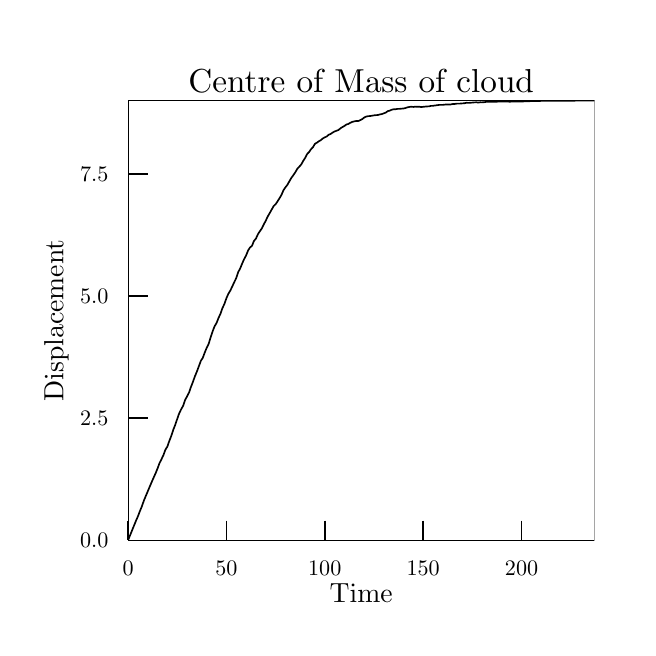
\begin{tikzpicture}[x=1pt,y=1pt]
\definecolor[named]{fillColor}{rgb}{1.00,1.00,1.00}
\path[use as bounding box,fill=fillColor,fill opacity=0.00] (0,0) rectangle (216.81,216.81);
\begin{scope}
\path[clip] (  0.00,  0.00) rectangle (216.81,216.81);
\definecolor[named]{drawColor}{rgb}{1.00,1.00,1.00}
\definecolor[named]{fillColor}{rgb}{1.00,1.00,1.00}

\path[draw=drawColor,line width= 0.6pt,line join=round,line cap=round,fill=fillColor] (  0.00,  0.00) rectangle (216.81,216.81);
\end{scope}
\begin{scope}
\path[clip] ( 36.27, 31.56) rectangle (204.77,190.48);
\definecolor[named]{fillColor}{rgb}{1.00,1.00,1.00}

\path[fill=fillColor] ( 36.27, 31.56) rectangle (204.76,190.48);
\definecolor[named]{drawColor}{rgb}{0.00,0.00,0.00}

\path[draw=drawColor,line width= 0.6pt,line join=round] ( 36.27, 31.56) --
	( 36.98, 33.32) --
	( 37.69, 35.07) --
	( 38.40, 36.82) --
	( 39.11, 38.58) --
	( 39.82, 40.19) --
	( 40.53, 42.06) --
	( 41.24, 43.77) --
	( 41.95, 45.81) --
	( 42.66, 47.54) --
	( 43.37, 49.20) --
	( 44.09, 50.93) --
	( 44.80, 52.59) --
	( 45.51, 54.21) --
	( 46.22, 55.78) --
	( 46.93, 57.53) --
	( 47.64, 59.47) --
	( 48.35, 60.87) --
	( 49.06, 62.37) --
	( 49.77, 64.31) --
	( 50.48, 65.44) --
	( 51.20, 67.52) --
	( 51.91, 69.34) --
	( 52.62, 71.53) --
	( 53.33, 73.32) --
	( 54.04, 75.42) --
	( 54.75, 77.45) --
	( 55.46, 78.91) --
	( 56.17, 80.15) --
	( 56.88, 82.23) --
	( 57.59, 83.59) --
	( 58.31, 84.97) --
	( 59.02, 87.02) --
	( 59.73, 88.87) --
	( 60.44, 90.85) --
	( 61.15, 92.56) --
	( 61.86, 94.47) --
	( 62.57, 96.40) --
	( 63.28, 97.51) --
	( 63.99, 99.42) --
	( 64.70,101.16) --
	( 65.41,102.59) --
	( 66.13,104.98) --
	( 66.84,107.10) --
	( 67.55,108.93) --
	( 68.26,110.10) --
	( 68.97,111.95) --
	( 69.68,113.44) --
	( 70.39,115.52) --
	( 71.10,116.98) --
	( 71.81,119.05) --
	( 72.52,120.64) --
	( 73.24,121.84) --
	( 73.95,123.34) --
	( 74.66,124.88) --
	( 75.37,126.33) --
	( 76.08,128.50) --
	( 76.79,129.82) --
	( 77.50,131.55) --
	( 78.21,133.18) --
	( 78.92,134.48) --
	( 79.63,136.27) --
	( 80.35,137.40) --
	( 81.06,137.98) --
	( 81.77,139.75) --
	( 82.48,140.59) --
	( 83.19,142.15) --
	( 83.90,143.26) --
	( 84.61,144.25) --
	( 85.32,145.73) --
	( 86.03,147.04) --
	( 86.74,148.59) --
	( 87.45,149.79) --
	( 88.17,151.08) --
	( 88.88,152.34) --
	( 89.59,153.01) --
	( 90.30,154.07) --
	( 91.01,155.20) --
	( 91.72,156.40) --
	( 92.43,158.08) --
	( 93.14,159.12) --
	( 93.85,160.02) --
	( 94.56,161.29) --
	( 95.28,162.53) --
	( 95.99,163.48) --
	( 96.70,164.54) --
	( 97.41,165.79) --
	( 98.12,166.55) --
	( 98.83,167.35) --
	( 99.54,168.63) --
	(100.25,169.73) --
	(100.96,171.12) --
	(101.67,171.85) --
	(102.39,172.91) --
	(103.10,173.63) --
	(103.81,174.85) --
	(104.52,175.26) --
	(105.23,175.77) --
	(105.94,176.17) --
	(106.65,176.79) --
	(107.36,177.16) --
	(108.07,177.50) --
	(108.78,178.12) --
	(109.50,178.40) --
	(110.21,178.93) --
	(110.92,179.30) --
	(111.63,179.57) --
	(112.34,179.85) --
	(113.05,180.47) --
	(113.76,180.91) --
	(114.47,181.30) --
	(115.18,181.83) --
	(115.89,182.02) --
	(116.60,182.46) --
	(117.32,182.76) --
	(118.03,182.96) --
	(118.74,183.10) --
	(119.45,183.06) --
	(120.16,183.38) --
	(120.87,183.75) --
	(121.58,184.32) --
	(122.29,184.67) --
	(123.00,184.83) --
	(123.71,184.88) --
	(124.43,184.99) --
	(125.14,185.13) --
	(125.85,185.20) --
	(126.56,185.25) --
	(127.27,185.46) --
	(127.98,185.60) --
	(128.69,185.85) --
	(129.40,186.12) --
	(130.11,186.65) --
	(130.82,186.82) --
	(131.54,187.16) --
	(132.25,187.32) --
	(132.96,187.35) --
	(133.67,187.46) --
	(134.38,187.48) --
	(135.09,187.55) --
	(135.80,187.60) --
	(136.51,187.76) --
	(137.22,188.02) --
	(137.93,188.16) --
	(138.64,188.25) --
	(139.36,188.16) --
	(140.07,188.27) --
	(140.78,188.22) --
	(141.49,188.24) --
	(142.20,188.13) --
	(142.91,188.20) --
	(143.62,188.29) --
	(144.33,188.34) --
	(145.04,188.39) --
	(145.75,188.55) --
	(146.47,188.57) --
	(147.18,188.69) --
	(147.89,188.78) --
	(148.60,188.89) --
	(149.31,188.92) --
	(150.02,188.91) --
	(150.73,189.01) --
	(151.44,189.07) --
	(152.15,189.07) --
	(152.86,189.07) --
	(153.58,189.21) --
	(154.29,189.24) --
	(155.00,189.35) --
	(155.71,189.37) --
	(156.42,189.38) --
	(157.13,189.45) --
	(157.84,189.51) --
	(158.55,189.67) --
	(159.26,189.63) --
	(159.97,189.67) --
	(160.68,189.74) --
	(161.40,189.81) --
	(162.11,189.84) --
	(162.82,189.75) --
	(163.53,189.84) --
	(164.24,189.82) --
	(164.95,189.88) --
	(165.66,190.00) --
	(166.37,190.00) --
	(167.08,190.02) --
	(167.79,190.02) --
	(168.51,190.05) --
	(169.22,190.02) --
	(169.93,190.09) --
	(170.64,190.09) --
	(171.35,190.11) --
	(172.06,190.12) --
	(172.77,190.12) --
	(173.48,190.11) --
	(174.19,190.04) --
	(174.90,190.11) --
	(175.62,190.11) --
	(176.33,190.14) --
	(177.04,190.11) --
	(177.75,190.11) --
	(178.46,190.11) --
	(179.17,190.16) --
	(179.88,190.16) --
	(180.59,190.20) --
	(181.30,190.23) --
	(182.01,190.28) --
	(182.72,190.30) --
	(183.44,190.28) --
	(184.15,190.30) --
	(184.86,190.32) --
	(185.57,190.35) --
	(186.28,190.35) --
	(186.99,190.37) --
	(187.70,190.37) --
	(188.41,190.35) --
	(189.12,190.39) --
	(189.83,190.35) --
	(190.55,190.35) --
	(191.26,190.39) --
	(191.97,190.39) --
	(192.68,190.41) --
	(193.39,190.41) --
	(194.10,190.42) --
	(194.81,190.42) --
	(195.52,190.42) --
	(196.23,190.41) --
	(196.94,190.42) --
	(197.66,190.42) --
	(198.37,190.46) --
	(199.08,190.44) --
	(199.79,190.44) --
	(200.50,190.44) --
	(201.21,190.44) --
	(201.92,190.44) --
	(202.63,190.46) --
	(203.34,190.46) --
	(204.05,190.46) --
	(204.77,190.48);

\path[draw=drawColor,line width= 0.6pt,line join=round,line cap=round] ( 36.27, 31.56) rectangle (204.76,190.48);
\end{scope}
\begin{scope}
\path[clip] (  0.00,  0.00) rectangle (216.81,216.81);
\definecolor[named]{drawColor}{rgb}{0.00,0.00,0.00}

\node[text=drawColor,anchor=base east,inner sep=0pt, outer sep=0pt, scale=  0.80] at ( 29.15, 28.80) {0.0};

\node[text=drawColor,anchor=base east,inner sep=0pt, outer sep=0pt, scale=  0.80] at ( 29.15, 72.95) {2.5};

\node[text=drawColor,anchor=base east,inner sep=0pt, outer sep=0pt, scale=  0.80] at ( 29.15,117.09) {5.0};

\node[text=drawColor,anchor=base east,inner sep=0pt, outer sep=0pt, scale=  0.80] at ( 29.15,161.24) {7.5};
\end{scope}
\begin{scope}
\path[clip] (  0.00,  0.00) rectangle (216.81,216.81);
\definecolor[named]{drawColor}{rgb}{0.00,0.00,0.00}

\path[draw=drawColor,line width= 0.6pt,line join=round] ( 43.38, 31.56) --
	( 36.27, 31.56);

\path[draw=drawColor,line width= 0.6pt,line join=round] ( 43.38, 75.70) --
	( 36.27, 75.70);

\path[draw=drawColor,line width= 0.6pt,line join=round] ( 43.38,119.85) --
	( 36.27,119.85);

\path[draw=drawColor,line width= 0.6pt,line join=round] ( 43.38,163.99) --
	( 36.27,163.99);
\end{scope}
\begin{scope}
\path[clip] (  0.00,  0.00) rectangle (216.81,216.81);
\definecolor[named]{drawColor}{rgb}{0.00,0.00,0.00}

\path[draw=drawColor,line width= 0.6pt,line join=round] ( 36.27, 38.67) --
	( 36.27, 31.56);

\path[draw=drawColor,line width= 0.6pt,line join=round] ( 71.81, 38.67) --
	( 71.81, 31.56);

\path[draw=drawColor,line width= 0.6pt,line join=round] (107.36, 38.67) --
	(107.36, 31.56);

\path[draw=drawColor,line width= 0.6pt,line join=round] (142.91, 38.67) --
	(142.91, 31.56);

\path[draw=drawColor,line width= 0.6pt,line join=round] (178.46, 38.67) --
	(178.46, 31.56);
\end{scope}
\begin{scope}
\path[clip] (  0.00,  0.00) rectangle (216.81,216.81);
\definecolor[named]{drawColor}{rgb}{0.00,0.00,0.00}

\node[text=drawColor,anchor=base,inner sep=0pt, outer sep=0pt, scale=  0.80] at ( 36.27, 18.93) {0};

\node[text=drawColor,anchor=base,inner sep=0pt, outer sep=0pt, scale=  0.80] at ( 71.81, 18.93) {50};

\node[text=drawColor,anchor=base,inner sep=0pt, outer sep=0pt, scale=  0.80] at (107.36, 18.93) {100};

\node[text=drawColor,anchor=base,inner sep=0pt, outer sep=0pt, scale=  0.80] at (142.91, 18.93) {150};

\node[text=drawColor,anchor=base,inner sep=0pt, outer sep=0pt, scale=  0.80] at (178.46, 18.93) {200};
\end{scope}
\begin{scope}
\path[clip] (  0.00,  0.00) rectangle (216.81,216.81);
\definecolor[named]{drawColor}{rgb}{0.00,0.00,0.00}

\node[text=drawColor,anchor=base,inner sep=0pt, outer sep=0pt, scale=  1.00] at (120.52,  9.03) {Time};
\end{scope}
\begin{scope}
\path[clip] (  0.00,  0.00) rectangle (216.81,216.81);
\definecolor[named]{drawColor}{rgb}{0.00,0.00,0.00}

\node[text=drawColor,rotate= 90.00,anchor=base,inner sep=0pt, outer sep=0pt, scale=  1.00] at ( 12.91,111.02) {Displacement};
\end{scope}
\begin{scope}
\path[clip] (  0.00,  0.00) rectangle (216.81,216.81);
\definecolor[named]{drawColor}{rgb}{0.00,0.00,0.00}

\node[text=drawColor,anchor=base,inner sep=0pt, outer sep=0pt, scale=  1.20] at (120.52,193.49) {Centre of Mass of cloud};
\end{scope}
\end{tikzpicture}
%
		\caption{}
		\label{fig:FlatDisp}
	\end{subfigure}%
	\begin{subfigure}[h]{ 0.5 \textwidth}	
			% Created by tikzDevice version 0.7.0 on 2014-12-02 17:54:13
% !TEX encoding = UTF-8 Unicode
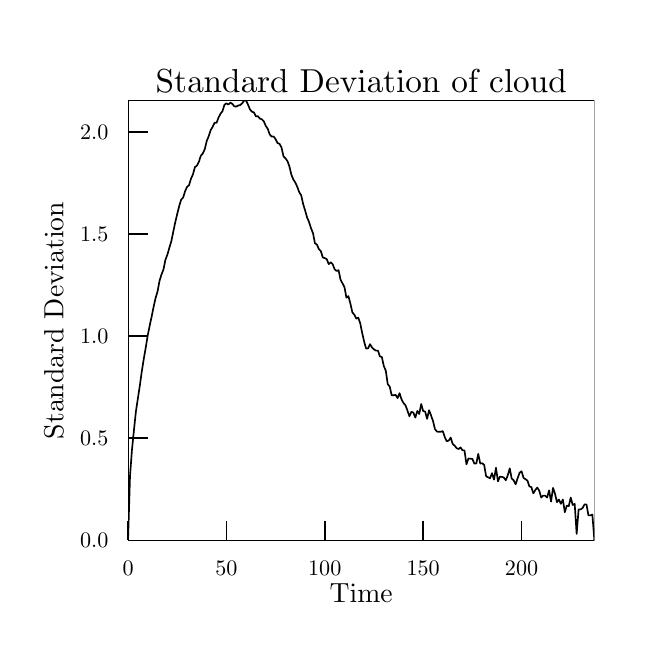
\begin{tikzpicture}[x=1pt,y=1pt]
\definecolor[named]{fillColor}{rgb}{1.00,1.00,1.00}
\path[use as bounding box,fill=fillColor,fill opacity=0.00] (0,0) rectangle (216.81,216.81);
\begin{scope}
\path[clip] (  0.00,  0.00) rectangle (216.81,216.81);
\definecolor[named]{drawColor}{rgb}{1.00,1.00,1.00}
\definecolor[named]{fillColor}{rgb}{1.00,1.00,1.00}

\path[draw=drawColor,line width= 0.6pt,line join=round,line cap=round,fill=fillColor] (  0.00,  0.00) rectangle (216.81,216.81);
\end{scope}
\begin{scope}
\path[clip] ( 36.27, 31.56) rectangle (204.77,190.48);
\definecolor[named]{fillColor}{rgb}{1.00,1.00,1.00}

\path[fill=fillColor] ( 36.27, 31.56) rectangle (204.76,190.48);
\definecolor[named]{drawColor}{rgb}{0.00,0.00,0.00}

\path[draw=drawColor,line width= 0.6pt,line join=round] ( 36.27, 31.56) --
	( 36.98, 54.76) --
	( 37.69, 64.33) --
	( 38.40, 71.36) --
	( 39.11, 78.13) --
	( 39.82, 82.81) --
	( 40.53, 87.49) --
	( 41.24, 92.61) --
	( 41.95, 97.11) --
	( 42.66,101.18) --
	( 43.37,105.58) --
	( 44.09,109.15) --
	( 44.80,112.38) --
	( 45.51,115.95) --
	( 46.22,119.13) --
	( 46.93,121.48) --
	( 47.64,125.31) --
	( 48.35,127.60) --
	( 49.06,129.41) --
	( 49.77,132.94) --
	( 50.48,134.76) --
	( 51.20,137.29) --
	( 51.91,139.65) --
	( 52.62,143.11) --
	( 53.33,146.49) --
	( 54.04,149.50) --
	( 54.75,152.34) --
	( 55.46,154.67) --
	( 56.17,155.39) --
	( 56.88,157.71) --
	( 57.59,159.28) --
	( 58.31,159.88) --
	( 59.02,162.25) --
	( 59.73,163.81) --
	( 60.44,166.42) --
	( 61.15,166.93) --
	( 61.86,168.31) --
	( 62.57,170.55) --
	( 63.28,171.33) --
	( 63.99,172.89) --
	( 64.70,175.85) --
	( 65.41,177.59) --
	( 66.13,179.82) --
	( 66.84,180.97) --
	( 67.55,182.49) --
	( 68.26,182.44) --
	( 68.97,184.34) --
	( 69.68,185.72) --
	( 70.39,186.60) --
	( 71.10,188.96) --
	( 71.81,189.45) --
	( 72.52,189.02) --
	( 73.24,189.71) --
	( 73.95,189.26) --
	( 74.66,188.39) --
	( 75.37,188.30) --
	( 76.08,188.69) --
	( 76.79,188.84) --
	( 77.50,189.46) --
	( 78.21,190.46) --
	( 78.92,190.48) --
	( 79.63,188.95) --
	( 80.35,187.23) --
	( 81.06,186.43) --
	( 81.77,186.18) --
	( 82.48,184.74) --
	( 83.19,184.80) --
	( 83.90,183.96) --
	( 84.61,183.71) --
	( 85.32,182.99) --
	( 86.03,181.31) --
	( 86.74,180.29) --
	( 87.45,178.26) --
	( 88.17,177.43) --
	( 88.88,177.48) --
	( 89.59,176.54) --
	( 90.30,175.09) --
	( 91.01,174.84) --
	( 91.72,173.50) --
	( 92.43,170.34) --
	( 93.14,169.59) --
	( 93.85,168.65) --
	( 94.56,166.72) --
	( 95.28,163.70) --
	( 95.99,161.96) --
	( 96.70,160.86) --
	( 97.41,159.33) --
	( 98.12,157.37) --
	( 98.83,156.26) --
	( 99.54,153.07) --
	(100.25,150.76) --
	(100.96,148.25) --
	(101.67,146.59) --
	(102.39,144.32) --
	(103.10,142.57) --
	(103.81,138.90) --
	(104.52,138.42) --
	(105.23,136.78) --
	(105.94,136.05) --
	(106.65,133.75) --
	(107.36,133.54) --
	(108.07,133.15) --
	(108.78,131.37) --
	(109.50,132.02) --
	(110.21,131.35) --
	(110.92,129.51) --
	(111.63,128.89) --
	(112.34,129.18) --
	(113.05,125.75) --
	(113.76,124.43) --
	(114.47,123.08) --
	(115.18,119.23) --
	(115.89,119.81) --
	(116.60,117.19) --
	(117.32,113.93) --
	(118.03,113.11) --
	(118.74,111.66) --
	(119.45,112.04) --
	(120.16,110.02) --
	(120.87,106.52) --
	(121.58,103.38) --
	(122.29,100.86) --
	(123.00,100.93) --
	(123.71,102.44) --
	(124.43,101.23) --
	(125.14,100.56) --
	(125.85,100.10) --
	(126.56,100.10) --
	(127.27, 98.04) --
	(127.98, 97.77) --
	(128.69, 94.55) --
	(129.40, 92.87) --
	(130.11, 88.02) --
	(130.82, 87.11) --
	(131.54, 83.96) --
	(132.25, 83.97) --
	(132.96, 84.11) --
	(133.67, 82.97) --
	(134.38, 84.75) --
	(135.09, 82.47) --
	(135.80, 81.17) --
	(136.51, 80.39) --
	(137.22, 78.48) --
	(137.93, 76.41) --
	(138.64, 77.98) --
	(139.36, 77.73) --
	(140.07, 75.90) --
	(140.78, 78.30) --
	(141.49, 77.20) --
	(142.20, 80.83) --
	(142.91, 78.29) --
	(143.62, 78.07) --
	(144.33, 75.47) --
	(145.04, 78.56) --
	(145.75, 76.73) --
	(146.47, 74.65) --
	(147.18, 71.74) --
	(147.89, 70.85) --
	(148.60, 70.79) --
	(149.31, 70.81) --
	(150.02, 71.01) --
	(150.73, 68.81) --
	(151.44, 67.36) --
	(152.15, 67.59) --
	(152.86, 68.70) --
	(153.58, 66.37) --
	(154.29, 65.77) --
	(155.00, 64.86) --
	(155.71, 64.55) --
	(156.42, 65.13) --
	(157.13, 64.10) --
	(157.84, 64.04) --
	(158.55, 59.04) --
	(159.26, 61.12) --
	(159.97, 61.05) --
	(160.68, 60.99) --
	(161.40, 59.31) --
	(162.11, 59.32) --
	(162.82, 62.79) --
	(163.53, 59.32) --
	(164.24, 59.41) --
	(164.95, 58.84) --
	(165.66, 54.68) --
	(166.37, 54.32) --
	(167.08, 53.97) --
	(167.79, 55.83) --
	(168.51, 53.49) --
	(169.22, 57.77) --
	(169.93, 52.87) --
	(170.64, 54.59) --
	(171.35, 54.48) --
	(172.06, 54.24) --
	(172.77, 53.26) --
	(173.48, 55.06) --
	(174.19, 57.57) --
	(174.90, 53.88) --
	(175.62, 53.26) --
	(176.33, 51.84) --
	(177.04, 54.00) --
	(177.75, 55.97) --
	(178.46, 56.52) --
	(179.17, 54.13) --
	(179.88, 53.64) --
	(180.59, 53.15) --
	(181.30, 51.04) --
	(182.01, 50.77) --
	(182.72, 48.52) --
	(183.44, 49.76) --
	(184.15, 50.63) --
	(184.86, 49.46) --
	(185.57, 47.02) --
	(186.28, 47.71) --
	(186.99, 47.71) --
	(187.70, 47.02) --
	(188.41, 49.62) --
	(189.12, 45.55) --
	(189.83, 50.50) --
	(190.55, 48.37) --
	(191.26, 45.35) --
	(191.97, 46.30) --
	(192.68, 44.75) --
	(193.39, 46.31) --
	(194.10, 41.72) --
	(194.81, 44.11) --
	(195.52, 43.90) --
	(196.23, 47.03) --
	(196.94, 44.33) --
	(197.66, 44.75) --
	(198.37, 33.89) --
	(199.08, 42.74) --
	(199.79, 42.74) --
	(200.50, 43.22) --
	(201.21, 44.54) --
	(201.92, 44.54) --
	(202.63, 40.59) --
	(203.34, 40.59) --
	(204.05, 40.89) --
	(204.77, 31.56);

\path[draw=drawColor,line width= 0.6pt,line join=round,line cap=round] ( 36.27, 31.56) rectangle (204.76,190.48);
\end{scope}
\begin{scope}
\path[clip] (  0.00,  0.00) rectangle (216.81,216.81);
\definecolor[named]{drawColor}{rgb}{0.00,0.00,0.00}

\node[text=drawColor,anchor=base east,inner sep=0pt, outer sep=0pt, scale=  0.80] at ( 29.15, 28.80) {0.0};

\node[text=drawColor,anchor=base east,inner sep=0pt, outer sep=0pt, scale=  0.80] at ( 29.15, 65.68) {0.5};

\node[text=drawColor,anchor=base east,inner sep=0pt, outer sep=0pt, scale=  0.80] at ( 29.15,102.56) {1.0};

\node[text=drawColor,anchor=base east,inner sep=0pt, outer sep=0pt, scale=  0.80] at ( 29.15,139.45) {1.5};

\node[text=drawColor,anchor=base east,inner sep=0pt, outer sep=0pt, scale=  0.80] at ( 29.15,176.33) {2.0};
\end{scope}
\begin{scope}
\path[clip] (  0.00,  0.00) rectangle (216.81,216.81);
\definecolor[named]{drawColor}{rgb}{0.00,0.00,0.00}

\path[draw=drawColor,line width= 0.6pt,line join=round] ( 43.38, 31.56) --
	( 36.27, 31.56);

\path[draw=drawColor,line width= 0.6pt,line join=round] ( 43.38, 68.44) --
	( 36.27, 68.44);

\path[draw=drawColor,line width= 0.6pt,line join=round] ( 43.38,105.32) --
	( 36.27,105.32);

\path[draw=drawColor,line width= 0.6pt,line join=round] ( 43.38,142.20) --
	( 36.27,142.20);

\path[draw=drawColor,line width= 0.6pt,line join=round] ( 43.38,179.08) --
	( 36.27,179.08);
\end{scope}
\begin{scope}
\path[clip] (  0.00,  0.00) rectangle (216.81,216.81);
\definecolor[named]{drawColor}{rgb}{0.00,0.00,0.00}

\path[draw=drawColor,line width= 0.6pt,line join=round] ( 36.27, 38.67) --
	( 36.27, 31.56);

\path[draw=drawColor,line width= 0.6pt,line join=round] ( 71.81, 38.67) --
	( 71.81, 31.56);

\path[draw=drawColor,line width= 0.6pt,line join=round] (107.36, 38.67) --
	(107.36, 31.56);

\path[draw=drawColor,line width= 0.6pt,line join=round] (142.91, 38.67) --
	(142.91, 31.56);

\path[draw=drawColor,line width= 0.6pt,line join=round] (178.46, 38.67) --
	(178.46, 31.56);
\end{scope}
\begin{scope}
\path[clip] (  0.00,  0.00) rectangle (216.81,216.81);
\definecolor[named]{drawColor}{rgb}{0.00,0.00,0.00}

\node[text=drawColor,anchor=base,inner sep=0pt, outer sep=0pt, scale=  0.80] at ( 36.27, 18.93) {0};

\node[text=drawColor,anchor=base,inner sep=0pt, outer sep=0pt, scale=  0.80] at ( 71.81, 18.93) {50};

\node[text=drawColor,anchor=base,inner sep=0pt, outer sep=0pt, scale=  0.80] at (107.36, 18.93) {100};

\node[text=drawColor,anchor=base,inner sep=0pt, outer sep=0pt, scale=  0.80] at (142.91, 18.93) {150};

\node[text=drawColor,anchor=base,inner sep=0pt, outer sep=0pt, scale=  0.80] at (178.46, 18.93) {200};
\end{scope}
\begin{scope}
\path[clip] (  0.00,  0.00) rectangle (216.81,216.81);
\definecolor[named]{drawColor}{rgb}{0.00,0.00,0.00}

\node[text=drawColor,anchor=base,inner sep=0pt, outer sep=0pt, scale=  1.00] at (120.52,  9.03) {Time};
\end{scope}
\begin{scope}
\path[clip] (  0.00,  0.00) rectangle (216.81,216.81);
\definecolor[named]{drawColor}{rgb}{0.00,0.00,0.00}

\node[text=drawColor,rotate= 90.00,anchor=base,inner sep=0pt, outer sep=0pt, scale=  1.00] at ( 12.91,111.02) {Standard Deviation};
\end{scope}
\begin{scope}
\path[clip] (  0.00,  0.00) rectangle (216.81,216.81);
\definecolor[named]{drawColor}{rgb}{0.00,0.00,0.00}

\node[text=drawColor,anchor=base,inner sep=0pt, outer sep=0pt, scale=  1.20] at (120.52,193.49) {Standard Deviation of cloud};
\end{scope}
\end{tikzpicture}
%
		\caption{}
		\label{fig:FlatVar}
	\end{subfigure}
	\caption{The statistics calculated from the cloud formed in figure \ref{fig:Cloud}.}	
	\label{fig:FlatStats}
\end{figure}

The displacement graph, figure \ref{fig:FlatDisp}, behaves linearly with respect to time until it reaches the end of the mutation landscape. This is due to the absorbing nature of the final mutation, in this case mutation number nine. No backward mutations can occur to states with less mutations, so the overall population of cells congregates to this final state. The peak of the standard deviation graph, figure \ref{fig:FlatVar}, shows that the cloud quickly diffuses and is most dispersed early on in the simulation before decreasing again as the cells move into the final state.

Overall, the extension to the model has produced a good starting point for further parameter variations and the formation of the cloud is a good milestone in the exploration of the dynamics of cancer evolution.

\section{Analytic Analysis}

It is now desirable to use the transition rates (equation  \eqref{eq:TransRate}) to derive a deterministic equation that describes the dynamics of the cloud. 

Firstly, a large number of cells limit is needed, such that the equations can be formed in terms of concentrations rather than population numbers

\begin{equation}
x _ i = \lim _{M \rightarrow \infty} \frac{n_i}{M}.
\label{eq:LargeCellAsumption}
\end{equation}

The change in concentration is now governed by the transition of cells into and out of the specific cell type. Therefore, the change in a particular concentration can be defined as; 

\begin{equation}
\dot{x} _i = \frac{1}{M} \sum _{j \neq i } \left( T^{j \rightarrow i } - T^{i \rightarrow j}  \right).
\end{equation}

Substituting in the transition rates, equation \eqref{eq:TransRate}, and taking the large cell limit, equation \eqref{eq:LargeCellAsumption}, lead to the general equation: 

\begin{equation}
\bar{r} \dot{x} _i = \sum _{j \neq i} \left( u_i r_{i-1} x_{i-1} + (1 - u_{i+1} ) r_i x_i \right) x_j - \left( u _j r_{j-1} x_{j-1} + (1 - u_{j+1} ) r _j x_j \right) x_i .
\end{equation}

By using the fact that the concentrations are normalised, $\sum _i x_i = 1 $ and the expression for the average fitness $ \sum _i r _i x _i = \bar{r}  $ the concentration evolution equation can be simplified to

\begin{equation}
\bar{r} \dot{x} _i = u_i r_{i-1} x_{i-1} + x _i ( r_i ( 1 - u_{i+1} ) - \bar{r} ),
\label{eq:MasterSimple}
\end{equation}

it is from this equation that all further work is derived from. 

\subsection{A Poissonian Solution}

For the simplest case, the fitness landscape and mutation probabilities are homogeneous

\begin{align}
r_i & = r \quad \forall i, \\
u_i & = u \quad  \forall i, \\
\bar{r} & = r.
\end{align}

Using these simplifications  and changing the label of $x _i$ to $\rho _i$ simplifies equation \eqref{eq:MasterSimple} to

\begin{equation}
\dot{\rho} _i  = u ( \rho _{i-1} - \rho _i ).
\label{eq:PoisMasterSimple}
\end{equation}

This characterises itself as a Poissonian process and therefore can be solved exactly.

By starting with $i=0$ and using the fact that $\rho _{-1} = 0$, a simple ordinary differential equation can be found and solved to produce

\begin{equation}
\rho _0 = e^{-ut} .
\end{equation}

The initial condition of $\rho _0 (t=0) = 1 $ is also used and shows that all the cells initially have zero mutations. 

Now we notice that it is possible to iteratively solve equation \eqref{eq:PoisMasterSimple} with a general solution

\begin{equation}
\rho _n  = \frac{(u t)^n}{n!} e^{-ut}.
\label{eq:PoisSolution}
\end{equation}

By using a proof by induction it possible to show that this is true for all $n$.
 
The final state, where the cell has achieved the maximum amount of mutations has a separate equation as it is an absorbing state, i.e. once a cell is in state $\rho _N$ it never leaves. Since $\rho _i$ represents a concentration, the final state contains the amount of concentration that is not in the non-absorbing states
\begin{equation}
\rho _N = 1 - \sum _{n=0} ^{N-1} \rho _n.
\label{eq:PoisSolutionFinal}
\end{equation}

We now wish to compare this analytic result with previous simulation data. 
 
\begin{figure}[H]
	\centering
		% Created by tikzDevice version 0.7.0 on 2014-12-04 14:55:38
% !TEX encoding = UTF-8 Unicode
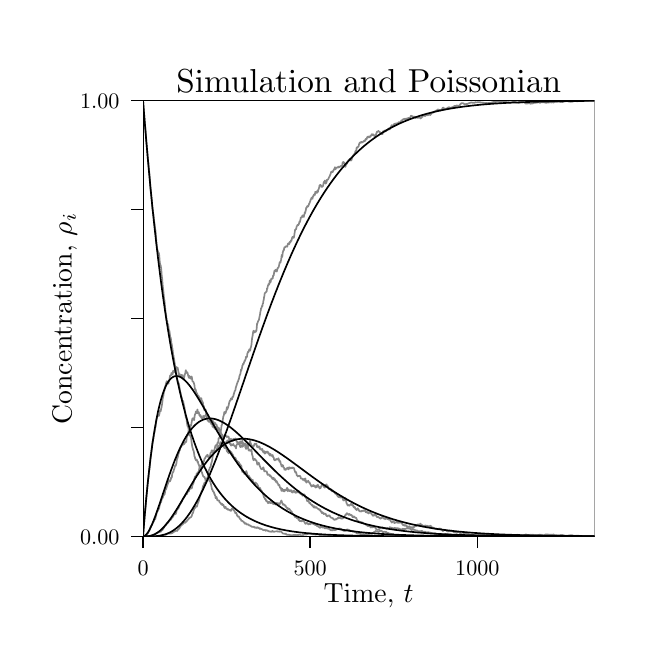
\begin{tikzpicture}[x=1pt,y=1pt]
\definecolor[named]{fillColor}{rgb}{1.00,1.00,1.00}
\path[use as bounding box,fill=fillColor,fill opacity=0.00] (0,0) rectangle (216.81,216.81);
\begin{scope}
\path[clip] (  0.00,  0.00) rectangle (216.81,216.81);
\definecolor[named]{drawColor}{rgb}{1.00,1.00,1.00}
\definecolor[named]{fillColor}{rgb}{1.00,1.00,1.00}

\path[draw=drawColor,line width= 0.6pt,line join=round,line cap=round,fill=fillColor] ( -0.00,  0.00) rectangle (216.81,216.81);
\end{scope}
\begin{scope}
\path[clip] ( 41.69, 32.98) rectangle (204.76,190.48);
\definecolor[named]{fillColor}{rgb}{1.00,1.00,1.00}

\path[fill=fillColor] ( 41.69, 32.98) rectangle (204.76,190.48);
\definecolor[named]{drawColor}{rgb}{0.53,0.53,0.53}

\path[draw=drawColor,line width= 0.6pt,line join=round] ( 41.69,190.48) --
	( 41.81,188.85) --
	( 41.93,187.49) --
	( 42.05,185.84) --
	( 42.17,184.27) --
	( 42.29,182.86) --
	( 42.41,181.64) --
	( 42.53,180.39) --
	( 42.65,179.15) --
	( 42.77,177.36) --
	( 42.89,175.61) --
	( 43.02,174.09) --
	( 43.14,172.74) --
	( 43.26,171.38) --
	( 43.38,169.97) --
	( 43.50,168.60) --
	( 43.62,167.99) --
	( 43.74,166.27) --
	( 43.86,165.10) --
	( 43.98,164.20) --
	( 44.10,162.89) --
	( 44.22,161.17) --
	( 44.34,159.17) --
	( 44.47,157.54) --
	( 44.59,156.70) --
	( 44.71,155.65) --
	( 44.83,154.46) --
	( 44.95,152.87) --
	( 45.07,151.56) --
	( 45.19,150.73) --
	( 45.31,149.77) --
	( 45.43,149.34) --
	( 45.55,148.36) --
	( 45.67,146.92) --
	( 45.79,146.28) --
	( 45.91,145.43) --
	( 46.04,144.26) --
	( 46.16,143.59) --
	( 46.28,142.55) --
	( 46.40,140.72) --
	( 46.52,139.30) --
	( 46.64,138.05) --
	( 46.76,137.08) --
	( 46.88,136.52) --
	( 47.00,136.20) --
	( 47.12,135.76) --
	( 47.24,134.62) --
	( 47.36,135.50) --
	( 47.49,134.94) --
	( 47.61,133.63) --
	( 47.73,132.14) --
	( 47.85,131.33) --
	( 47.97,131.06) --
	( 48.09,130.76) --
	( 48.21,129.97) --
	( 48.33,128.73) --
	( 48.45,127.07) --
	( 48.57,126.46) --
	( 48.69,124.88) --
	( 48.81,123.40) --
	( 48.93,122.49) --
	( 49.06,121.35) --
	( 49.18,120.04) --
	( 49.30,118.89) --
	( 49.42,118.32) --
	( 49.54,117.16) --
	( 49.66,115.74) --
	( 49.78,114.58) --
	( 49.90,113.63) --
	( 50.02,113.10) --
	( 50.14,111.82) --
	( 50.26,110.97) --
	( 50.38,110.93) --
	( 50.51,109.89) --
	( 50.63,109.71) --
	( 50.75,109.67) --
	( 50.87,108.76) --
	( 50.99,107.68) --
	( 51.11,107.33) --
	( 51.23,107.21) --
	( 51.35,106.22) --
	( 51.47,105.38) --
	( 51.59,104.70) --
	( 51.71,104.73) --
	( 51.83,103.70) --
	( 51.95,102.72) --
	( 52.08,102.42) --
	( 52.20,101.19) --
	( 52.32,100.80) --
	( 52.44, 99.96) --
	( 52.56, 98.63) --
	( 52.68, 98.38) --
	( 52.80, 97.46) --
	( 52.92, 97.07) --
	( 53.04, 96.03) --
	( 53.16, 95.43) --
	( 53.28, 94.07) --
	( 53.40, 94.02) --
	( 53.53, 93.68) --
	( 53.65, 92.49) --
	( 53.77, 91.76) --
	( 53.89, 90.02) --
	( 54.01, 89.85) --
	( 54.13, 89.23) --
	( 54.25, 88.59) --
	( 54.37, 88.76) --
	( 54.49, 88.34) --
	( 54.61, 88.30) --
	( 54.73, 87.71) --
	( 54.85, 86.88) --
	( 54.97, 86.18) --
	( 55.10, 85.23) --
	( 55.22, 85.01) --
	( 55.34, 84.31) --
	( 55.46, 83.49) --
	( 55.58, 82.92) --
	( 55.70, 83.27) --
	( 55.82, 82.26) --
	( 55.94, 81.49) --
	( 56.06, 81.89) --
	( 56.18, 81.91) --
	( 56.30, 81.15) --
	( 56.42, 80.67) --
	( 56.55, 80.06) --
	( 56.67, 79.52) --
	( 56.79, 78.56) --
	( 56.91, 77.86) --
	( 57.03, 76.81) --
	( 57.15, 75.87) --
	( 57.27, 76.21) --
	( 57.39, 75.57) --
	( 57.51, 74.37) --
	( 57.63, 73.54) --
	( 57.75, 72.80) --
	( 57.87, 73.02) --
	( 57.99, 72.48) --
	( 58.12, 71.93) --
	( 58.24, 71.66) --
	( 58.36, 70.25) --
	( 58.48, 69.58) --
	( 58.60, 69.55) --
	( 58.72, 69.46) --
	( 58.84, 69.05) --
	( 58.96, 68.85) --
	( 59.08, 68.40) --
	( 59.20, 67.17) --
	( 59.32, 66.42) --
	( 59.44, 65.52) --
	( 59.57, 64.96) --
	( 59.69, 64.72) --
	( 59.81, 64.05) --
	( 59.93, 64.01) --
	( 60.05, 63.51) --
	( 60.17, 62.70) --
	( 60.29, 61.77) --
	( 60.41, 61.76) --
	( 60.53, 60.98) --
	( 60.65, 61.09) --
	( 60.77, 60.49) --
	( 60.89, 60.69) --
	( 61.01, 60.61) --
	( 61.14, 60.65) --
	( 61.26, 60.13) --
	( 61.38, 59.85) --
	( 61.50, 60.08) --
	( 61.62, 59.23) --
	( 61.74, 59.16) --
	( 61.86, 58.80) --
	( 61.98, 58.58) --
	( 62.10, 58.01) --
	( 62.22, 57.79) --
	( 62.34, 57.81) --
	( 62.46, 56.85) --
	( 62.58, 57.23) --
	( 62.71, 56.75) --
	( 62.83, 56.28) --
	( 62.95, 56.20) --
	( 63.07, 55.63) --
	( 63.19, 55.40) --
	( 63.31, 54.98) --
	( 63.43, 54.71) --
	( 63.55, 54.61) --
	( 63.67, 54.48) --
	( 63.79, 54.51) --
	( 63.91, 54.42) --
	( 64.03, 54.10) --
	( 64.16, 53.85) --
	( 64.28, 52.89) --
	( 64.40, 52.60) --
	( 64.52, 52.85) --
	( 64.64, 53.02) --
	( 64.76, 53.16) --
	( 64.88, 53.50) --
	( 65.00, 53.71) --
	( 65.12, 53.74) --
	( 65.24, 53.83) --
	( 65.36, 53.75) --
	( 65.48, 53.56) --
	( 65.60, 53.26) --
	( 65.73, 52.96) --
	( 65.85, 52.91) --
	( 65.97, 52.87) --
	( 66.09, 52.31) --
	( 66.21, 51.96) --
	( 66.33, 51.35) --
	( 66.45, 50.82) --
	( 66.57, 49.99) --
	( 66.69, 50.06) --
	( 66.81, 49.80) --
	( 66.93, 49.26) --
	( 67.05, 49.20) --
	( 67.18, 49.11) --
	( 67.30, 48.96) --
	( 67.42, 48.31) --
	( 67.54, 48.36) --
	( 67.66, 47.75) --
	( 67.78, 47.80) --
	( 67.90, 46.83) --
	( 68.02, 46.79) --
	( 68.14, 47.02) --
	( 68.26, 47.22) --
	( 68.38, 46.69) --
	( 68.50, 46.14) --
	( 68.62, 46.03) --
	( 68.75, 46.11) --
	( 68.87, 45.87) --
	( 68.99, 45.94) --
	( 69.11, 45.95) --
	( 69.23, 45.84) --
	( 69.35, 45.26) --
	( 69.47, 45.22) --
	( 69.59, 45.12) --
	( 69.71, 45.01) --
	( 69.83, 44.87) --
	( 69.95, 44.60) --
	( 70.07, 44.83) --
	( 70.20, 44.82) --
	( 70.32, 44.31) --
	( 70.44, 44.45) --
	( 70.56, 44.25) --
	( 70.68, 44.45) --
	( 70.80, 44.24) --
	( 70.92, 43.79) --
	( 71.04, 43.51) --
	( 71.16, 43.26) --
	( 71.28, 43.39) --
	( 71.40, 43.64) --
	( 71.52, 43.67) --
	( 71.64, 43.18) --
	( 71.77, 42.99) --
	( 71.89, 43.02) --
	( 72.01, 42.84) --
	( 72.13, 42.96) --
	( 72.25, 43.01) --
	( 72.37, 42.60) --
	( 72.49, 42.55) --
	( 72.61, 42.73) --
	( 72.73, 42.57) --
	( 72.85, 42.59) --
	( 72.97, 42.57) --
	( 73.09, 42.36) --
	( 73.22, 42.57) --
	( 73.34, 42.21) --
	( 73.46, 42.19) --
	( 73.58, 42.40) --
	( 73.70, 42.77) --
	( 73.82, 43.01) --
	( 73.94, 43.12) --
	( 74.06, 42.74) --
	( 74.18, 42.85) --
	( 74.30, 42.68) --
	( 74.42, 42.54) --
	( 74.54, 42.37) --
	( 74.66, 42.24) --
	( 74.79, 41.90) --
	( 74.91, 41.88) --
	( 75.03, 41.36) --
	( 75.15, 41.47) --
	( 75.27, 41.53) --
	( 75.39, 41.53) --
	( 75.51, 41.07) --
	( 75.63, 40.55) --
	( 75.75, 40.60) --
	( 75.87, 40.15) --
	( 75.99, 40.11) --
	( 76.11, 40.14) --
	( 76.24, 40.23) --
	( 76.36, 39.99) --
	( 76.48, 39.77) --
	( 76.60, 39.54) --
	( 76.72, 39.36) --
	( 76.84, 39.17) --
	( 76.96, 39.21) --
	( 77.08, 38.98) --
	( 77.20, 38.64) --
	( 77.32, 38.54) --
	( 77.44, 38.65) --
	( 77.56, 38.56) --
	( 77.68, 38.46) --
	( 77.81, 38.37) --
	( 77.93, 38.30) --
	( 78.05, 38.11) --
	( 78.17, 37.91) --
	( 78.29, 38.05) --
	( 78.41, 38.01) --
	( 78.53, 37.54) --
	( 78.65, 37.64) --
	( 78.77, 37.57) --
	( 78.89, 37.72) --
	( 79.01, 37.39) --
	( 79.13, 37.32) --
	( 79.26, 37.29) --
	( 79.38, 37.33) --
	( 79.50, 37.37) --
	( 79.62, 37.33) --
	( 79.74, 37.20) --
	( 79.86, 37.18) --
	( 79.98, 37.05) --
	( 80.10, 36.91) --
	( 80.22, 36.82) --
	( 80.34, 36.95) --
	( 80.46, 36.82) --
	( 80.58, 36.79) --
	( 80.70, 36.70) --
	( 80.83, 36.61) --
	( 80.95, 36.45) --
	( 81.07, 36.37) --
	( 81.19, 36.52) --
	( 81.31, 36.37) --
	( 81.43, 36.42) --
	( 81.55, 36.41) --
	( 81.67, 36.47) --
	( 81.79, 36.44) --
	( 81.91, 36.23) --
	( 82.03, 36.30) --
	( 82.15, 36.07) --
	( 82.28, 36.17) --
	( 82.40, 36.17) --
	( 82.52, 36.22) --
	( 82.64, 36.25) --
	( 82.76, 36.05) --
	( 82.88, 36.03) --
	( 83.00, 36.29) --
	( 83.12, 36.13) --
	( 83.24, 36.00) --
	( 83.36, 36.15) --
	( 83.48, 36.01) --
	( 83.60, 35.97) --
	( 83.72, 35.85) --
	( 83.85, 35.68) --
	( 83.97, 35.91) --
	( 84.09, 35.76) --
	( 84.21, 35.66) --
	( 84.33, 35.67) --
	( 84.45, 35.71) --
	( 84.57, 35.61) --
	( 84.69, 35.55) --
	( 84.81, 35.54) --
	( 84.93, 35.42) --
	( 85.05, 35.36) --
	( 85.17, 35.17) --
	( 85.30, 35.25) --
	( 85.42, 35.25) --
	( 85.54, 35.20) --
	( 85.66, 35.34) --
	( 85.78, 35.33) --
	( 85.90, 35.15) --
	( 86.02, 35.01) --
	( 86.14, 35.15) --
	( 86.26, 35.20) --
	( 86.38, 35.20) --
	( 86.50, 35.15) --
	( 86.62, 35.00) --
	( 86.74, 35.10) --
	( 86.87, 35.02) --
	( 86.99, 34.84) --
	( 87.11, 34.79) --
	( 87.23, 34.82) --
	( 87.35, 34.80) --
	( 87.47, 34.72) --
	( 87.59, 34.80) --
	( 87.71, 34.71) --
	( 87.83, 34.70) --
	( 87.95, 34.66) --
	( 88.07, 34.74) --
	( 88.19, 34.66) --
	( 88.32, 34.88) --
	( 88.44, 34.97) --
	( 88.56, 34.90) --
	( 88.68, 34.69) --
	( 88.80, 34.68) --
	( 88.92, 34.75) --
	( 89.04, 34.66) --
	( 89.16, 34.69) --
	( 89.28, 34.72) --
	( 89.40, 34.75) --
	( 89.52, 34.79) --
	( 89.64, 34.81) --
	( 89.76, 34.79) --
	( 89.89, 34.79) --
	( 90.01, 34.87) --
	( 90.13, 34.87) --
	( 90.25, 34.76) --
	( 90.37, 34.68) --
	( 90.49, 34.80) --
	( 90.61, 34.76) --
	( 90.73, 34.76) --
	( 90.85, 34.65) --
	( 90.97, 34.68) --
	( 91.09, 34.89) --
	( 91.21, 34.71) --
	( 91.34, 34.77) --
	( 91.46, 34.69) --
	( 91.58, 34.73) --
	( 91.70, 34.60) --
	( 91.82, 34.41) --
	( 91.94, 34.38) --
	( 92.06, 34.23) --
	( 92.18, 34.08) --
	( 92.30, 34.01) --
	( 92.42, 33.95) --
	( 92.54, 34.04) --
	( 92.66, 33.96) --
	( 92.78, 33.93) --
	( 92.91, 33.94) --
	( 93.03, 33.89) --
	( 93.15, 34.04) --
	( 93.27, 33.97) --
	( 93.39, 33.75) --
	( 93.51, 33.61) --
	( 93.63, 33.60) --
	( 93.75, 33.56) --
	( 93.87, 33.59) --
	( 93.99, 33.49) --
	( 94.11, 33.56) --
	( 94.23, 33.63) --
	( 94.36, 33.50) --
	( 94.48, 33.53) --
	( 94.60, 33.58) --
	( 94.72, 33.51) --
	( 94.84, 33.44) --
	( 94.96, 33.43) --
	( 95.08, 33.42) --
	( 95.20, 33.34) --
	( 95.32, 33.40) --
	( 95.44, 33.39) --
	( 95.56, 33.39) --
	( 95.68, 33.39) --
	( 95.80, 33.41) --
	( 95.93, 33.50) --
	( 96.05, 33.48) --
	( 96.17, 33.45) --
	( 96.29, 33.48) --
	( 96.41, 33.48) --
	( 96.53, 33.48) --
	( 96.65, 33.49) --
	( 96.77, 33.56) --
	( 96.89, 33.49) --
	( 97.01, 33.49) --
	( 97.13, 33.43) --
	( 97.25, 33.44) --
	( 97.38, 33.44) --
	( 97.50, 33.51) --
	( 97.62, 33.52) --
	( 97.74, 33.50) --
	( 97.86, 33.50) --
	( 97.98, 33.54) --
	( 98.10, 33.52) --
	( 98.22, 33.60) --
	( 98.34, 33.61) --
	( 98.46, 33.52) --
	( 98.58, 33.40) --
	( 98.70, 33.43) --
	( 98.82, 33.38) --
	( 98.95, 33.36) --
	( 99.07, 33.36) --
	( 99.19, 33.39) --
	( 99.31, 33.44) --
	( 99.43, 33.46) --
	( 99.55, 33.48) --
	( 99.67, 33.51) --
	( 99.79, 33.58) --
	( 99.91, 33.62) --
	(100.03, 33.61) --
	(100.15, 33.63) --
	(100.27, 33.66) --
	(100.39, 33.71) --
	(100.52, 33.72) --
	(100.64, 33.62) --
	(100.76, 33.70) --
	(100.88, 33.74) --
	(101.00, 33.78) --
	(101.12, 33.88) --
	(101.24, 33.89) --
	(101.36, 33.88) --
	(101.48, 33.90) --
	(101.60, 33.98) --
	(101.72, 34.07) --
	(101.84, 34.14) --
	(101.97, 34.00) --
	(102.09, 34.00) --
	(102.21, 33.98) --
	(102.33, 34.01) --
	(102.45, 33.90) --
	(102.57, 33.83) --
	(102.69, 33.79) --
	(102.81, 33.78) --
	(102.93, 33.84) --
	(103.05, 33.72) --
	(103.17, 33.72) --
	(103.29, 33.72) --
	(103.41, 33.70) --
	(103.54, 33.72) --
	(103.66, 33.73) --
	(103.78, 33.69) --
	(103.90, 33.68) --
	(104.02, 33.59) --
	(104.14, 33.63) --
	(104.26, 33.66) --
	(104.38, 33.70) --
	(104.50, 33.78) --
	(104.62, 33.74) --
	(104.74, 33.73) --
	(104.86, 33.67) --
	(104.99, 33.68) --
	(105.11, 33.75) --
	(105.23, 33.59) --
	(105.35, 33.58) --
	(105.47, 33.48) --
	(105.59, 33.41) --
	(105.71, 33.35) --
	(105.83, 33.37) --
	(105.95, 33.38) --
	(106.07, 33.37) --
	(106.19, 33.40) --
	(106.31, 33.33) --
	(106.43, 33.27) --
	(106.56, 33.28) --
	(106.68, 33.26) --
	(106.80, 33.30) --
	(106.92, 33.30) --
	(107.04, 33.27) --
	(107.16, 33.23) --
	(107.28, 33.23) --
	(107.40, 33.20) --
	(107.52, 33.20) --
	(107.64, 33.21) --
	(107.76, 33.23) --
	(107.88, 33.24) --
	(108.01, 33.22) --
	(108.13, 33.24) --
	(108.25, 33.24) --
	(108.37, 33.23) --
	(108.49, 33.23) --
	(108.61, 33.19) --
	(108.73, 33.18) --
	(108.85, 33.16) --
	(108.97, 33.18) --
	(109.09, 33.20) --
	(109.21, 33.22) --
	(109.33, 33.23) --
	(109.45, 33.23) --
	(109.58, 33.24) --
	(109.70, 33.22) --
	(109.82, 33.25) --
	(109.94, 33.22) --
	(110.06, 33.32) --
	(110.18, 33.39) --
	(110.30, 33.47) --
	(110.42, 33.41) --
	(110.54, 33.47) --
	(110.66, 33.36) --
	(110.78, 33.35) --
	(110.90, 33.36) --
	(111.03, 33.23) --
	(111.15, 33.24) --
	(111.27, 33.35) --
	(111.39, 33.32) --
	(111.51, 33.35) --
	(111.63, 33.27) --
	(111.75, 33.27) --
	(111.87, 33.29) --
	(111.99, 33.26) --
	(112.11, 33.23) --
	(112.23, 33.22) --
	(112.35, 33.24) --
	(112.47, 33.25) --
	(112.60, 33.20) --
	(112.72, 33.18) --
	(112.84, 33.20) --
	(112.96, 33.19) --
	(113.08, 33.25) --
	(113.20, 33.18) --
	(113.32, 33.18) --
	(113.44, 33.22) --
	(113.56, 33.22) --
	(113.68, 33.23) --
	(113.80, 33.23) --
	(113.92, 33.26) --
	(114.05, 33.25) --
	(114.17, 33.28) --
	(114.29, 33.29) --
	(114.41, 33.21) --
	(114.53, 33.18) --
	(114.65, 33.19) --
	(114.77, 33.25) --
	(114.89, 33.28) --
	(115.01, 33.21) --
	(115.13, 33.20) --
	(115.25, 33.15) --
	(115.37, 33.14) --
	(115.49, 33.10) --
	(115.62, 33.08) --
	(115.74, 33.08) --
	(115.86, 33.09) --
	(115.98, 33.12) --
	(116.10, 33.09) --
	(116.22, 33.09) --
	(116.34, 33.07) --
	(116.46, 33.08) --
	(116.58, 33.09) --
	(116.70, 33.09) --
	(116.82, 33.12) --
	(116.94, 33.11) --
	(117.07, 33.11) --
	(117.19, 33.09) --
	(117.31, 33.09) --
	(117.43, 33.12) --
	(117.55, 33.06) --
	(117.67, 33.03) --
	(117.79, 33.08) --
	(117.91, 33.04) --
	(118.03, 33.04) --
	(118.15, 33.03) --
	(118.27, 33.04) --
	(118.39, 33.08) --
	(118.51, 33.11) --
	(118.64, 33.12) --
	(118.76, 33.11) --
	(118.88, 33.12) --
	(119.00, 33.09) --
	(119.12, 33.10) --
	(119.24, 33.09) --
	(119.36, 33.08) --
	(119.48, 33.12) --
	(119.60, 33.15) --
	(119.72, 33.10) --
	(119.84, 33.05) --
	(119.96, 33.05) --
	(120.09, 33.05) --
	(120.21, 33.07) --
	(120.33, 33.06) --
	(120.45, 33.04) --
	(120.57, 33.04) --
	(120.69, 33.04) --
	(120.81, 33.04) --
	(120.93, 33.03) --
	(121.05, 33.02) --
	(121.17, 33.01) --
	(121.29, 33.00) --
	(121.41, 33.00) --
	(121.53, 33.00) --
	(121.66, 32.98) --
	(121.78, 32.98) --
	(121.90, 32.98) --
	(122.02, 32.98) --
	(122.14, 32.98) --
	(122.26, 32.98) --
	(122.38, 32.98) --
	(122.50, 32.98) --
	(122.62, 32.98) --
	(122.74, 32.98) --
	(122.86, 32.98) --
	(122.98, 32.98) --
	(123.11, 32.98) --
	(123.23, 32.98) --
	(123.35, 32.98) --
	(123.47, 32.98) --
	(123.59, 32.98) --
	(123.71, 32.98) --
	(123.83, 32.98) --
	(123.95, 32.98) --
	(124.07, 32.98) --
	(124.19, 32.98) --
	(124.31, 32.98) --
	(124.43, 32.98) --
	(124.55, 32.98) --
	(124.68, 32.98) --
	(124.80, 32.98) --
	(124.92, 32.98) --
	(125.04, 32.98) --
	(125.16, 32.98) --
	(125.28, 32.98) --
	(125.40, 32.98) --
	(125.52, 32.98) --
	(125.64, 32.98) --
	(125.76, 32.98) --
	(125.88, 32.98) --
	(126.00, 32.98) --
	(126.13, 32.98) --
	(126.25, 32.98) --
	(126.37, 32.98) --
	(126.49, 32.98) --
	(126.61, 32.98) --
	(126.73, 32.98) --
	(126.85, 32.98) --
	(126.97, 32.98) --
	(127.09, 32.98) --
	(127.21, 32.98) --
	(127.33, 32.98) --
	(127.45, 32.98) --
	(127.57, 32.98) --
	(127.70, 32.98) --
	(127.82, 32.98) --
	(127.94, 32.98) --
	(128.06, 32.98) --
	(128.18, 32.98) --
	(128.30, 32.98) --
	(128.42, 32.98) --
	(128.54, 32.98) --
	(128.66, 32.98) --
	(128.78, 32.98) --
	(128.90, 32.98) --
	(129.02, 32.98) --
	(129.15, 32.98) --
	(129.27, 32.98) --
	(129.39, 32.98) --
	(129.51, 32.98) --
	(129.63, 32.98) --
	(129.75, 32.98) --
	(129.87, 32.98) --
	(129.99, 32.98) --
	(130.11, 32.98) --
	(130.23, 32.98) --
	(130.35, 32.98) --
	(130.47, 32.98) --
	(130.59, 32.98) --
	(130.72, 32.98) --
	(130.84, 32.98) --
	(130.96, 32.98) --
	(131.08, 32.98) --
	(131.20, 32.98) --
	(131.32, 32.98) --
	(131.44, 32.98) --
	(131.56, 32.98) --
	(131.68, 32.98) --
	(131.80, 32.98) --
	(131.92, 32.98) --
	(132.04, 32.98) --
	(132.17, 32.98) --
	(132.29, 32.98) --
	(132.41, 32.98) --
	(132.53, 32.98) --
	(132.65, 32.98) --
	(132.77, 32.98) --
	(132.89, 32.98) --
	(133.01, 32.98) --
	(133.13, 32.98) --
	(133.25, 32.98) --
	(133.37, 32.98) --
	(133.49, 32.98) --
	(133.61, 32.98) --
	(133.74, 32.98) --
	(133.86, 32.98) --
	(133.98, 32.98) --
	(134.10, 32.98) --
	(134.22, 32.98) --
	(134.34, 32.98) --
	(134.46, 32.98) --
	(134.58, 32.98) --
	(134.70, 32.98) --
	(134.82, 32.98) --
	(134.94, 32.98) --
	(135.06, 32.98) --
	(135.18, 32.98) --
	(135.31, 32.98) --
	(135.43, 32.98) --
	(135.55, 32.98) --
	(135.67, 32.98) --
	(135.79, 32.98) --
	(135.91, 32.98) --
	(136.03, 32.98) --
	(136.15, 32.98) --
	(136.27, 32.98) --
	(136.39, 32.98) --
	(136.51, 32.98) --
	(136.63, 32.98) --
	(136.76, 32.98) --
	(136.88, 32.98) --
	(137.00, 32.98) --
	(137.12, 32.98) --
	(137.24, 32.98) --
	(137.36, 32.98) --
	(137.48, 32.98) --
	(137.60, 32.98) --
	(137.72, 32.98) --
	(137.84, 32.98) --
	(137.96, 32.98) --
	(138.08, 32.98) --
	(138.20, 32.98) --
	(138.33, 32.98) --
	(138.45, 32.98) --
	(138.57, 32.98) --
	(138.69, 32.98) --
	(138.81, 32.98) --
	(138.93, 32.98) --
	(139.05, 32.98) --
	(139.17, 32.98) --
	(139.29, 32.98) --
	(139.41, 32.98) --
	(139.53, 32.98) --
	(139.65, 32.98) --
	(139.78, 32.98) --
	(139.90, 32.98) --
	(140.02, 32.98) --
	(140.14, 32.98) --
	(140.26, 32.98) --
	(140.38, 32.98) --
	(140.50, 32.98) --
	(140.62, 32.98) --
	(140.74, 32.98) --
	(140.86, 32.98) --
	(140.98, 32.98) --
	(141.10, 32.98) --
	(141.22, 32.98) --
	(141.35, 32.98) --
	(141.47, 32.98) --
	(141.59, 32.98) --
	(141.71, 32.98) --
	(141.83, 32.98) --
	(141.95, 32.98) --
	(142.07, 32.98) --
	(142.19, 32.98) --
	(142.31, 32.98) --
	(142.43, 32.98) --
	(142.55, 32.98) --
	(142.67, 32.98) --
	(142.80, 32.98) --
	(142.92, 32.98) --
	(143.04, 32.98) --
	(143.16, 32.98) --
	(143.28, 32.98) --
	(143.40, 32.98) --
	(143.52, 32.98) --
	(143.64, 32.98) --
	(143.76, 32.98) --
	(143.88, 32.98) --
	(144.00, 32.98) --
	(144.12, 32.98) --
	(144.24, 32.98) --
	(144.37, 32.98) --
	(144.49, 32.98) --
	(144.61, 32.98) --
	(144.73, 32.98) --
	(144.85, 32.98) --
	(144.97, 32.98) --
	(145.09, 32.98) --
	(145.21, 32.98) --
	(145.33, 32.98) --
	(145.45, 32.98) --
	(145.57, 32.98) --
	(145.69, 32.98) --
	(145.82, 32.98) --
	(145.94, 32.98) --
	(146.06, 32.98) --
	(146.18, 32.98) --
	(146.30, 32.98) --
	(146.42, 32.98) --
	(146.54, 32.98) --
	(146.66, 32.98) --
	(146.78, 32.98) --
	(146.90, 32.98) --
	(147.02, 32.98) --
	(147.14, 32.98) --
	(147.26, 32.98) --
	(147.39, 32.98) --
	(147.51, 32.98) --
	(147.63, 32.98) --
	(147.75, 32.98) --
	(147.87, 32.98) --
	(147.99, 32.98) --
	(148.11, 32.98) --
	(148.23, 32.98) --
	(148.35, 32.98) --
	(148.47, 32.98) --
	(148.59, 32.98) --
	(148.71, 32.98) --
	(148.84, 32.98) --
	(148.96, 32.98) --
	(149.08, 32.98) --
	(149.20, 32.98) --
	(149.32, 32.98) --
	(149.44, 32.98) --
	(149.56, 32.98) --
	(149.68, 32.98) --
	(149.80, 32.98) --
	(149.92, 32.98) --
	(150.04, 32.98) --
	(150.16, 32.98) --
	(150.28, 32.98) --
	(150.41, 32.98) --
	(150.53, 32.98) --
	(150.65, 32.98) --
	(150.77, 32.98) --
	(150.89, 32.98) --
	(151.01, 32.98) --
	(151.13, 32.98) --
	(151.25, 32.98) --
	(151.37, 32.98) --
	(151.49, 32.98) --
	(151.61, 32.98) --
	(151.73, 32.98) --
	(151.86, 32.98) --
	(151.98, 32.98) --
	(152.10, 32.98) --
	(152.22, 32.98) --
	(152.34, 32.98) --
	(152.46, 32.98) --
	(152.58, 32.98) --
	(152.70, 32.98) --
	(152.82, 32.98) --
	(152.94, 32.98) --
	(153.06, 32.98) --
	(153.18, 32.98) --
	(153.30, 32.98) --
	(153.43, 32.98) --
	(153.55, 32.98) --
	(153.67, 32.98) --
	(153.79, 32.98) --
	(153.91, 32.98) --
	(154.03, 32.98) --
	(154.15, 32.98) --
	(154.27, 32.98) --
	(154.39, 32.98) --
	(154.51, 32.98) --
	(154.63, 32.98) --
	(154.75, 32.98) --
	(154.88, 32.98) --
	(155.00, 32.98) --
	(155.12, 32.98) --
	(155.24, 32.98) --
	(155.36, 32.98) --
	(155.48, 32.98) --
	(155.60, 32.98) --
	(155.72, 32.98) --
	(155.84, 32.98) --
	(155.96, 32.98) --
	(156.08, 32.98) --
	(156.20, 32.98) --
	(156.32, 32.98) --
	(156.45, 32.98) --
	(156.57, 32.98) --
	(156.69, 32.98) --
	(156.81, 32.98) --
	(156.93, 32.98) --
	(157.05, 32.98) --
	(157.17, 32.98) --
	(157.29, 32.98) --
	(157.41, 32.98) --
	(157.53, 32.98) --
	(157.65, 32.98) --
	(157.77, 32.98) --
	(157.90, 32.98) --
	(158.02, 32.98) --
	(158.14, 32.98) --
	(158.26, 32.98) --
	(158.38, 32.98) --
	(158.50, 32.98) --
	(158.62, 32.98) --
	(158.74, 32.98) --
	(158.86, 32.98) --
	(158.98, 32.98) --
	(159.10, 32.98) --
	(159.22, 32.98) --
	(159.34, 32.98) --
	(159.47, 32.98) --
	(159.59, 32.98) --
	(159.71, 32.98) --
	(159.83, 32.98) --
	(159.95, 32.98) --
	(160.07, 32.98) --
	(160.19, 32.98) --
	(160.31, 32.98) --
	(160.43, 32.98) --
	(160.55, 32.98) --
	(160.67, 32.98) --
	(160.79, 32.98) --
	(160.92, 32.98) --
	(161.04, 32.98) --
	(161.16, 32.98) --
	(161.28, 32.98) --
	(161.40, 32.98) --
	(161.52, 32.98) --
	(161.64, 32.98) --
	(161.76, 32.98) --
	(161.88, 32.98) --
	(162.00, 32.98) --
	(162.12, 32.98) --
	(162.24, 32.98) --
	(162.36, 32.98) --
	(162.49, 32.98) --
	(162.61, 32.98) --
	(162.73, 32.98) --
	(162.85, 32.98) --
	(162.97, 32.98) --
	(163.09, 32.98) --
	(163.21, 32.98) --
	(163.33, 32.98) --
	(163.45, 32.98) --
	(163.57, 32.98) --
	(163.69, 32.98) --
	(163.81, 32.98) --
	(163.94, 32.98) --
	(164.06, 32.98) --
	(164.18, 32.98) --
	(164.30, 32.98) --
	(164.42, 32.98) --
	(164.54, 32.98) --
	(164.66, 32.98) --
	(164.78, 32.98) --
	(164.90, 32.98) --
	(165.02, 32.98) --
	(165.14, 32.98) --
	(165.26, 32.98) --
	(165.38, 32.98) --
	(165.51, 32.98) --
	(165.63, 32.98) --
	(165.75, 32.98) --
	(165.87, 32.98) --
	(165.99, 32.98) --
	(166.11, 32.98) --
	(166.23, 32.98) --
	(166.35, 32.98) --
	(166.47, 32.98) --
	(166.59, 32.98) --
	(166.71, 32.98) --
	(166.83, 32.98) --
	(166.96, 32.98) --
	(167.08, 32.98) --
	(167.20, 32.98) --
	(167.32, 32.98) --
	(167.44, 32.98) --
	(167.56, 32.98) --
	(167.68, 32.98) --
	(167.80, 32.98) --
	(167.92, 32.98) --
	(168.04, 32.98) --
	(168.16, 32.98) --
	(168.28, 32.98) --
	(168.40, 32.98) --
	(168.53, 32.98) --
	(168.65, 32.98) --
	(168.77, 32.98) --
	(168.89, 32.98) --
	(169.01, 32.98) --
	(169.13, 32.98) --
	(169.25, 32.98) --
	(169.37, 32.98) --
	(169.49, 32.98) --
	(169.61, 32.98) --
	(169.73, 32.98) --
	(169.85, 32.98) --
	(169.97, 32.98) --
	(170.10, 32.98) --
	(170.22, 32.98) --
	(170.34, 32.98) --
	(170.46, 32.98) --
	(170.58, 32.98) --
	(170.70, 32.98) --
	(170.82, 32.98) --
	(170.94, 32.98) --
	(171.06, 32.98) --
	(171.18, 32.98) --
	(171.30, 32.98) --
	(171.42, 32.98) --
	(171.55, 32.98) --
	(171.67, 32.98) --
	(171.79, 32.98) --
	(171.91, 32.98) --
	(172.03, 32.98) --
	(172.15, 32.98) --
	(172.27, 32.98) --
	(172.39, 32.98) --
	(172.51, 32.98) --
	(172.63, 32.98) --
	(172.75, 32.98) --
	(172.87, 32.98) --
	(172.99, 32.98) --
	(173.12, 32.98) --
	(173.24, 32.98) --
	(173.36, 32.98) --
	(173.48, 32.98) --
	(173.60, 32.98) --
	(173.72, 32.98) --
	(173.84, 32.98) --
	(173.96, 32.98) --
	(174.08, 32.98) --
	(174.20, 32.98) --
	(174.32, 32.98) --
	(174.44, 32.98) --
	(174.57, 32.98) --
	(174.69, 32.98) --
	(174.81, 32.98) --
	(174.93, 32.98) --
	(175.05, 32.98) --
	(175.17, 32.98) --
	(175.29, 32.98) --
	(175.41, 32.98) --
	(175.53, 32.98) --
	(175.65, 32.98) --
	(175.77, 32.98) --
	(175.89, 32.98) --
	(176.01, 32.98) --
	(176.14, 32.98) --
	(176.26, 32.98) --
	(176.38, 32.98) --
	(176.50, 32.98) --
	(176.62, 32.98) --
	(176.74, 32.98) --
	(176.86, 32.98) --
	(176.98, 32.98) --
	(177.10, 32.98) --
	(177.22, 32.98) --
	(177.34, 32.98) --
	(177.46, 32.98) --
	(177.59, 32.98) --
	(177.71, 32.98) --
	(177.83, 32.98) --
	(177.95, 32.98) --
	(178.07, 32.98) --
	(178.19, 32.98) --
	(178.31, 32.98) --
	(178.43, 32.98) --
	(178.55, 32.98) --
	(178.67, 32.98) --
	(178.79, 32.98) --
	(178.91, 32.98) --
	(179.03, 32.98) --
	(179.16, 32.98) --
	(179.28, 32.98) --
	(179.40, 32.98) --
	(179.52, 32.98) --
	(179.64, 32.98) --
	(179.76, 32.98) --
	(179.88, 32.98) --
	(180.00, 32.98) --
	(180.12, 32.98) --
	(180.24, 32.98) --
	(180.36, 32.98) --
	(180.48, 32.98) --
	(180.61, 32.98) --
	(180.73, 32.98) --
	(180.85, 32.98) --
	(180.97, 32.98) --
	(181.09, 32.98) --
	(181.21, 32.98) --
	(181.33, 32.98) --
	(181.45, 32.98) --
	(181.57, 32.98) --
	(181.69, 32.98) --
	(181.81, 32.98) --
	(181.93, 32.98) --
	(182.05, 32.98) --
	(182.18, 32.98) --
	(182.30, 32.98) --
	(182.42, 32.98) --
	(182.54, 32.98) --
	(182.66, 32.98) --
	(182.78, 32.98) --
	(182.90, 32.98) --
	(183.02, 32.98) --
	(183.14, 32.98) --
	(183.26, 32.98) --
	(183.38, 32.98) --
	(183.50, 32.98) --
	(183.63, 32.98) --
	(183.75, 32.98) --
	(183.87, 32.98) --
	(183.99, 32.98) --
	(184.11, 32.98) --
	(184.23, 32.98) --
	(184.35, 32.98) --
	(184.47, 32.98) --
	(184.59, 32.98) --
	(184.71, 32.98) --
	(184.83, 32.98) --
	(184.95, 32.98) --
	(185.07, 32.98) --
	(185.20, 32.98) --
	(185.32, 32.98) --
	(185.44, 32.98) --
	(185.56, 32.98) --
	(185.68, 32.98) --
	(185.80, 32.98) --
	(185.92, 32.98) --
	(186.04, 32.98) --
	(186.16, 32.98) --
	(186.28, 32.98) --
	(186.40, 32.98) --
	(186.52, 32.98) --
	(186.65, 32.98) --
	(186.77, 32.98) --
	(186.89, 32.98) --
	(187.01, 32.98) --
	(187.13, 32.98) --
	(187.25, 32.98) --
	(187.37, 32.98) --
	(187.49, 32.98) --
	(187.61, 32.98) --
	(187.73, 32.98) --
	(187.85, 32.98) --
	(187.97, 32.98) --
	(188.09, 32.98) --
	(188.22, 32.98) --
	(188.34, 32.98) --
	(188.46, 32.98) --
	(188.58, 32.98) --
	(188.70, 32.98) --
	(188.82, 32.98) --
	(188.94, 32.98) --
	(189.06, 32.98) --
	(189.18, 32.98) --
	(189.30, 32.98) --
	(189.42, 32.98) --
	(189.54, 32.98) --
	(189.67, 32.98) --
	(189.79, 32.98) --
	(189.91, 32.98) --
	(190.03, 32.98) --
	(190.15, 32.98) --
	(190.27, 32.98) --
	(190.39, 32.98) --
	(190.51, 32.98) --
	(190.63, 32.98) --
	(190.75, 32.98) --
	(190.87, 32.98) --
	(190.99, 32.98) --
	(191.11, 32.98) --
	(191.24, 32.98) --
	(191.36, 32.98) --
	(191.48, 32.98) --
	(191.60, 32.98) --
	(191.72, 32.98) --
	(191.84, 32.98) --
	(191.96, 32.98) --
	(192.08, 32.98) --
	(192.20, 32.98) --
	(192.32, 32.98) --
	(192.44, 32.98) --
	(192.56, 32.98) --
	(192.69, 32.98) --
	(192.81, 32.98) --
	(192.93, 32.98) --
	(193.05, 32.98) --
	(193.17, 32.98) --
	(193.29, 32.98) --
	(193.41, 32.98) --
	(193.53, 32.98) --
	(193.65, 32.98) --
	(193.77, 32.98) --
	(193.89, 32.98) --
	(194.01, 32.98) --
	(194.13, 32.98) --
	(194.26, 32.98) --
	(194.38, 32.98) --
	(194.50, 32.98) --
	(194.62, 32.98) --
	(194.74, 32.98) --
	(194.86, 32.98) --
	(194.98, 32.98) --
	(195.10, 32.98) --
	(195.22, 32.98) --
	(195.34, 32.98) --
	(195.46, 32.98) --
	(195.58, 32.98) --
	(195.71, 32.98) --
	(195.83, 32.98) --
	(195.95, 32.98) --
	(196.07, 32.98) --
	(196.19, 32.98) --
	(196.31, 32.98) --
	(196.43, 32.98) --
	(196.55, 32.98) --
	(196.67, 32.98) --
	(196.79, 32.98) --
	(196.91, 32.98) --
	(197.03, 32.98) --
	(197.15, 32.98) --
	(197.28, 32.98) --
	(197.40, 32.98) --
	(197.52, 32.98) --
	(197.64, 32.98) --
	(197.76, 32.98) --
	(197.88, 32.98) --
	(198.00, 32.98) --
	(198.12, 32.98) --
	(198.24, 32.98) --
	(198.36, 32.98) --
	(198.48, 32.98) --
	(198.60, 32.98) --
	(198.73, 32.98) --
	(198.85, 32.98) --
	(198.97, 32.98) --
	(199.09, 32.98) --
	(199.21, 32.98) --
	(199.33, 32.98) --
	(199.45, 32.98) --
	(199.57, 32.98) --
	(199.69, 32.98) --
	(199.81, 32.98) --
	(199.93, 32.98) --
	(200.05, 32.98) --
	(200.17, 32.98) --
	(200.30, 32.98) --
	(200.42, 32.98) --
	(200.54, 32.98) --
	(200.66, 32.98) --
	(200.78, 32.98) --
	(200.90, 32.98) --
	(201.02, 32.98) --
	(201.14, 32.98) --
	(201.26, 32.98) --
	(201.38, 32.98) --
	(201.50, 32.98) --
	(201.62, 32.98) --
	(201.75, 32.98) --
	(201.87, 32.98) --
	(201.99, 32.98) --
	(202.11, 32.98) --
	(202.23, 32.98) --
	(202.35, 32.98) --
	(202.47, 32.98) --
	(202.59, 32.98) --
	(202.71, 32.98) --
	(202.83, 32.98) --
	(202.95, 32.98) --
	(203.07, 32.98) --
	(203.19, 32.98) --
	(203.32, 32.98) --
	(203.44, 32.98) --
	(203.56, 32.98) --
	(203.68, 32.98) --
	(203.80, 32.98) --
	(203.92, 32.98) --
	(204.04, 32.98) --
	(204.16, 32.98) --
	(204.28, 32.98) --
	(204.40, 32.98) --
	(204.52, 32.98) --
	(204.64, 32.98) --
	(204.76, 32.98);

\path[draw=drawColor,line width= 0.6pt,line join=round] ( 41.69, 32.98) --
	( 41.81, 34.60) --
	( 41.93, 35.94) --
	( 42.05, 37.55) --
	( 42.17, 39.11) --
	( 42.29, 40.46) --
	( 42.41, 41.66) --
	( 42.53, 42.79) --
	( 42.65, 43.92) --
	( 42.77, 45.54) --
	( 42.89, 47.12) --
	( 43.02, 48.50) --
	( 43.14, 49.64) --
	( 43.26, 50.90) --
	( 43.38, 52.33) --
	( 43.50, 53.63) --
	( 43.62, 53.97) --
	( 43.74, 55.33) --
	( 43.86, 56.39) --
	( 43.98, 57.00) --
	( 44.10, 57.93) --
	( 44.22, 59.25) --
	( 44.34, 60.80) --
	( 44.47, 62.13) --
	( 44.59, 62.77) --
	( 44.71, 63.71) --
	( 44.83, 64.73) --
	( 44.95, 65.85) --
	( 45.07, 66.94) --
	( 45.19, 67.37) --
	( 45.31, 67.97) --
	( 45.43, 68.27) --
	( 45.55, 69.13) --
	( 45.67, 70.21) --
	( 45.79, 70.38) --
	( 45.91, 70.90) --
	( 46.04, 72.13) --
	( 46.16, 72.40) --
	( 46.28, 72.85) --
	( 46.40, 74.21) --
	( 46.52, 74.96) --
	( 46.64, 75.61) --
	( 46.76, 75.99) --
	( 46.88, 76.46) --
	( 47.00, 76.68) --
	( 47.12, 76.67) --
	( 47.24, 76.99) --
	( 47.36, 76.49) --
	( 47.49, 76.70) --
	( 47.61, 77.28) --
	( 47.73, 78.16) --
	( 47.85, 78.49) --
	( 47.97, 78.20) --
	( 48.09, 78.25) --
	( 48.21, 79.08) --
	( 48.33, 79.47) --
	( 48.45, 80.14) --
	( 48.57, 80.81) --
	( 48.69, 81.81) --
	( 48.81, 82.98) --
	( 48.93, 83.38) --
	( 49.06, 83.88) --
	( 49.18, 84.92) --
	( 49.30, 85.58) --
	( 49.42, 85.60) --
	( 49.54, 86.67) --
	( 49.66, 86.94) --
	( 49.78, 87.42) --
	( 49.90, 87.76) --
	( 50.02, 88.42) --
	( 50.14, 88.72) --
	( 50.26, 89.07) --
	( 50.38, 88.44) --
	( 50.51, 88.99) --
	( 50.63, 89.00) --
	( 50.75, 88.52) --
	( 50.87, 88.18) --
	( 50.99, 89.09) --
	( 51.11, 89.32) --
	( 51.23, 89.64) --
	( 51.35, 90.43) --
	( 51.47, 91.08) --
	( 51.59, 91.16) --
	( 51.71, 91.24) --
	( 51.83, 91.21) --
	( 51.95, 92.03) --
	( 52.08, 91.88) --
	( 52.20, 91.90) --
	( 52.32, 91.47) --
	( 52.44, 91.94) --
	( 52.56, 92.86) --
	( 52.68, 92.65) --
	( 52.80, 92.58) --
	( 52.92, 92.30) --
	( 53.04, 92.83) --
	( 53.16, 92.89) --
	( 53.28, 93.69) --
	( 53.40, 94.08) --
	( 53.53, 93.82) --
	( 53.65, 94.25) --
	( 53.77, 94.02) --
	( 53.89, 94.16) --
	( 54.01, 93.77) --
	( 54.13, 93.91) --
	( 54.25, 93.84) --
	( 54.37, 92.93) --
	( 54.49, 92.40) --
	( 54.61, 91.89) --
	( 54.73, 91.22) --
	( 54.85, 91.62) --
	( 54.97, 91.60) --
	( 55.10, 91.20) --
	( 55.22, 90.87) --
	( 55.34, 90.94) --
	( 55.46, 91.26) --
	( 55.58, 91.31) --
	( 55.70, 90.77) --
	( 55.82, 91.14) --
	( 55.94, 91.23) --
	( 56.06, 90.52) --
	( 56.18, 90.01) --
	( 56.30, 89.66) --
	( 56.42, 89.97) --
	( 56.55, 90.63) --
	( 56.67, 90.93) --
	( 56.79, 91.56) --
	( 56.91, 91.70) --
	( 57.03, 92.46) --
	( 57.15, 93.04) --
	( 57.27, 92.43) --
	( 57.39, 92.06) --
	( 57.51, 92.29) --
	( 57.63, 92.33) --
	( 57.75, 92.13) --
	( 57.87, 91.62) --
	( 57.99, 91.08) --
	( 58.12, 90.77) --
	( 58.24, 90.26) --
	( 58.36, 90.92) --
	( 58.48, 90.93) --
	( 58.60, 90.71) --
	( 58.72, 90.14) --
	( 58.84, 90.18) --
	( 58.96, 89.95) --
	( 59.08, 90.44) --
	( 59.20, 90.75) --
	( 59.32, 90.56) --
	( 59.44, 89.66) --
	( 59.57, 89.02) --
	( 59.69, 88.88) --
	( 59.81, 88.89) --
	( 59.93, 88.72) --
	( 60.05, 88.38) --
	( 60.17, 88.06) --
	( 60.29, 87.36) --
	( 60.41, 86.04) --
	( 60.53, 86.28) --
	( 60.65, 86.07) --
	( 60.77, 85.77) --
	( 60.89, 85.17) --
	( 61.01, 84.85) --
	( 61.14, 84.75) --
	( 61.26, 84.51) --
	( 61.38, 83.53) --
	( 61.50, 83.68) --
	( 61.62, 83.76) --
	( 61.74, 83.88) --
	( 61.86, 83.30) --
	( 61.98, 83.21) --
	( 62.10, 83.20) --
	( 62.22, 82.25) --
	( 62.34, 82.16) --
	( 62.46, 82.42) --
	( 62.58, 82.62) --
	( 62.71, 82.92) --
	( 62.83, 82.56) --
	( 62.95, 81.63) --
	( 63.07, 81.90) --
	( 63.19, 81.32) --
	( 63.31, 81.44) --
	( 63.43, 80.25) --
	( 63.55, 79.90) --
	( 63.67, 80.10) --
	( 63.79, 78.92) --
	( 63.91, 78.51) --
	( 64.03, 78.74) --
	( 64.16, 78.45) --
	( 64.28, 78.90) --
	( 64.40, 78.27) --
	( 64.52, 77.42) --
	( 64.64, 77.07) --
	( 64.76, 75.73) --
	( 64.88, 75.55) --
	( 65.00, 74.86) --
	( 65.12, 74.89) --
	( 65.24, 74.78) --
	( 65.36, 74.41) --
	( 65.48, 74.54) --
	( 65.60, 74.47) --
	( 65.73, 74.55) --
	( 65.85, 74.52) --
	( 65.97, 74.76) --
	( 66.09, 74.65) --
	( 66.21, 74.48) --
	( 66.33, 74.69) --
	( 66.45, 73.76) --
	( 66.57, 74.09) --
	( 66.69, 73.43) --
	( 66.81, 72.61) --
	( 66.93, 72.92) --
	( 67.05, 72.51) --
	( 67.18, 72.46) --
	( 67.30, 72.26) --
	( 67.42, 72.56) --
	( 67.54, 72.60) --
	( 67.66, 72.44) --
	( 67.78, 71.73) --
	( 67.90, 72.44) --
	( 68.02, 72.65) --
	( 68.14, 72.28) --
	( 68.26, 71.98) --
	( 68.38, 72.32) --
	( 68.50, 72.65) --
	( 68.62, 72.33) --
	( 68.75, 72.18) --
	( 68.87, 71.65) --
	( 68.99, 71.14) --
	( 69.11, 71.26) --
	( 69.23, 71.54) --
	( 69.35, 71.16) --
	( 69.47, 70.94) --
	( 69.59, 70.94) --
	( 69.71, 70.08) --
	( 69.83, 69.37) --
	( 69.95, 69.05) --
	( 70.07, 68.76) --
	( 70.20, 68.78) --
	( 70.32, 68.42) --
	( 70.44, 67.39) --
	( 70.56, 66.79) --
	( 70.68, 66.02) --
	( 70.80, 65.95) --
	( 70.92, 65.40) --
	( 71.04, 64.94) --
	( 71.16, 65.37) --
	( 71.28, 64.98) --
	( 71.40, 64.87) --
	( 71.52, 65.16) --
	( 71.64, 64.97) --
	( 71.77, 64.71) --
	( 71.89, 64.22) --
	( 72.01, 63.67) --
	( 72.13, 63.89) --
	( 72.25, 63.37) --
	( 72.37, 63.63) --
	( 72.49, 63.22) --
	( 72.61, 63.02) --
	( 72.73, 63.44) --
	( 72.85, 63.57) --
	( 72.97, 63.41) --
	( 73.09, 63.95) --
	( 73.22, 63.40) --
	( 73.34, 63.19) --
	( 73.46, 63.32) --
	( 73.58, 63.46) --
	( 73.70, 63.19) --
	( 73.82, 62.70) --
	( 73.94, 62.18) --
	( 74.06, 62.69) --
	( 74.18, 62.26) --
	( 74.30, 62.14) --
	( 74.42, 61.45) --
	( 74.54, 61.61) --
	( 74.66, 61.54) --
	( 74.79, 61.22) --
	( 74.91, 61.34) --
	( 75.03, 61.41) --
	( 75.15, 61.10) --
	( 75.27, 60.88) --
	( 75.39, 60.37) --
	( 75.51, 60.39) --
	( 75.63, 60.34) --
	( 75.75, 59.95) --
	( 75.87, 59.66) --
	( 75.99, 60.04) --
	( 76.11, 59.69) --
	( 76.24, 59.54) --
	( 76.36, 59.79) --
	( 76.48, 58.86) --
	( 76.60, 58.75) --
	( 76.72, 59.10) --
	( 76.84, 58.98) --
	( 76.96, 58.70) --
	( 77.08, 58.20) --
	( 77.20, 58.52) --
	( 77.32, 57.65) --
	( 77.44, 56.89) --
	( 77.56, 56.26) --
	( 77.68, 57.05) --
	( 77.81, 56.41) --
	( 77.93, 56.28) --
	( 78.05, 56.08) --
	( 78.17, 56.11) --
	( 78.29, 55.54) --
	( 78.41, 55.67) --
	( 78.53, 56.03) --
	( 78.65, 56.28) --
	( 78.77, 56.24) --
	( 78.89, 56.07) --
	( 79.01, 56.60) --
	( 79.13, 56.19) --
	( 79.26, 55.75) --
	( 79.38, 54.72) --
	( 79.50, 54.69) --
	( 79.62, 54.88) --
	( 79.74, 54.89) --
	( 79.86, 54.99) --
	( 79.98, 54.66) --
	( 80.10, 54.61) --
	( 80.22, 54.33) --
	( 80.34, 53.98) --
	( 80.46, 54.06) --
	( 80.58, 53.87) --
	( 80.70, 53.67) --
	( 80.83, 53.65) --
	( 80.95, 53.08) --
	( 81.07, 53.25) --
	( 81.19, 53.28) --
	( 81.31, 53.38) --
	( 81.43, 52.89) --
	( 81.55, 52.72) --
	( 81.67, 52.39) --
	( 81.79, 52.23) --
	( 81.91, 52.29) --
	( 82.03, 52.27) --
	( 82.15, 51.98) --
	( 82.28, 52.19) --
	( 82.40, 52.45) --
	( 82.52, 52.11) --
	( 82.64, 52.16) --
	( 82.76, 52.04) --
	( 82.88, 51.87) --
	( 83.00, 51.79) --
	( 83.12, 51.34) --
	( 83.24, 51.24) --
	( 83.36, 50.88) --
	( 83.48, 50.53) --
	( 83.60, 50.32) --
	( 83.72, 50.03) --
	( 83.85, 50.46) --
	( 83.97, 50.50) --
	( 84.09, 50.10) --
	( 84.21, 49.83) --
	( 84.33, 49.53) --
	( 84.45, 49.50) --
	( 84.57, 49.42) --
	( 84.69, 48.97) --
	( 84.81, 48.84) --
	( 84.93, 48.56) --
	( 85.05, 48.43) --
	( 85.17, 47.91) --
	( 85.30, 47.39) --
	( 85.42, 47.09) --
	( 85.54, 47.13) --
	( 85.66, 46.51) --
	( 85.78, 46.60) --
	( 85.90, 46.61) --
	( 86.02, 46.36) --
	( 86.14, 45.91) --
	( 86.26, 45.68) --
	( 86.38, 45.73) --
	( 86.50, 45.50) --
	( 86.62, 45.72) --
	( 86.74, 45.23) --
	( 86.87, 44.95) --
	( 86.99, 45.14) --
	( 87.11, 45.25) --
	( 87.23, 45.37) --
	( 87.35, 45.51) --
	( 87.47, 45.22) --
	( 87.59, 45.04) --
	( 87.71, 45.40) --
	( 87.83, 45.32) --
	( 87.95, 45.00) --
	( 88.07, 45.08) --
	( 88.19, 45.16) --
	( 88.32, 45.23) --
	( 88.44, 45.34) --
	( 88.56, 45.16) --
	( 88.68, 44.69) --
	( 88.80, 44.86) --
	( 88.92, 44.67) --
	( 89.04, 45.13) --
	( 89.16, 44.82) --
	( 89.28, 44.71) --
	( 89.40, 44.88) --
	( 89.52, 44.48) --
	( 89.64, 44.85) --
	( 89.76, 44.72) --
	( 89.89, 45.00) --
	( 90.01, 45.05) --
	( 90.13, 45.02) --
	( 90.25, 44.95) --
	( 90.37, 44.77) --
	( 90.49, 45.00) --
	( 90.61, 44.82) --
	( 90.73, 44.83) --
	( 90.85, 44.60) --
	( 90.97, 44.48) --
	( 91.09, 44.63) --
	( 91.21, 45.06) --
	( 91.34, 45.20) --
	( 91.46, 45.52) --
	( 91.58, 45.74) --
	( 91.70, 45.96) --
	( 91.82, 45.59) --
	( 91.94, 45.15) --
	( 92.06, 44.86) --
	( 92.18, 44.88) --
	( 92.30, 44.37) --
	( 92.42, 44.53) --
	( 92.54, 44.49) --
	( 92.66, 44.48) --
	( 92.78, 44.49) --
	( 92.91, 44.05) --
	( 93.03, 44.19) --
	( 93.15, 44.06) --
	( 93.27, 43.95) --
	( 93.39, 43.59) --
	( 93.51, 43.47) --
	( 93.63, 43.43) --
	( 93.75, 43.12) --
	( 93.87, 42.89) --
	( 93.99, 43.25) --
	( 94.11, 42.90) --
	( 94.23, 42.76) --
	( 94.36, 43.00) --
	( 94.48, 42.99) --
	( 94.60, 42.82) --
	( 94.72, 42.52) --
	( 94.84, 42.55) --
	( 94.96, 42.33) --
	( 95.08, 42.13) --
	( 95.20, 42.05) --
	( 95.32, 41.97) --
	( 95.44, 41.84) --
	( 95.56, 41.37) --
	( 95.68, 41.19) --
	( 95.80, 41.19) --
	( 95.93, 41.03) --
	( 96.05, 40.91) --
	( 96.17, 40.86) --
	( 96.29, 40.65) --
	( 96.41, 40.38) --
	( 96.53, 40.14) --
	( 96.65, 39.95) --
	( 96.77, 39.89) --
	( 96.89, 40.01) --
	( 97.01, 39.95) --
	( 97.13, 39.79) --
	( 97.25, 39.54) --
	( 97.38, 39.56) --
	( 97.50, 39.53) --
	( 97.62, 39.58) --
	( 97.74, 39.50) --
	( 97.86, 38.96) --
	( 97.98, 38.91) --
	( 98.10, 38.97) --
	( 98.22, 38.62) --
	( 98.34, 38.50) --
	( 98.46, 38.51) --
	( 98.58, 38.57) --
	( 98.70, 38.59) --
	( 98.82, 38.68) --
	( 98.95, 38.40) --
	( 99.07, 38.63) --
	( 99.19, 38.50) --
	( 99.31, 38.70) --
	( 99.43, 38.67) --
	( 99.55, 38.69) --
	( 99.67, 38.72) --
	( 99.79, 38.49) --
	( 99.91, 38.27) --
	(100.03, 38.12) --
	(100.15, 37.90) --
	(100.27, 37.73) --
	(100.39, 37.49) --
	(100.52, 37.63) --
	(100.64, 37.72) --
	(100.76, 37.87) --
	(100.88, 37.73) --
	(101.00, 37.84) --
	(101.12, 37.78) --
	(101.24, 37.55) --
	(101.36, 37.39) --
	(101.48, 37.30) --
	(101.60, 37.48) --
	(101.72, 37.44) --
	(101.84, 37.46) --
	(101.97, 37.45) --
	(102.09, 37.42) --
	(102.21, 37.37) --
	(102.33, 37.60) --
	(102.45, 37.60) --
	(102.57, 37.70) --
	(102.69, 37.89) --
	(102.81, 37.88) --
	(102.93, 37.79) --
	(103.05, 37.52) --
	(103.17, 37.68) --
	(103.29, 37.52) --
	(103.41, 37.38) --
	(103.54, 37.29) --
	(103.66, 37.30) --
	(103.78, 37.30) --
	(103.90, 37.07) --
	(104.02, 37.26) --
	(104.14, 37.25) --
	(104.26, 37.01) --
	(104.38, 37.00) --
	(104.50, 36.85) --
	(104.62, 36.66) --
	(104.74, 36.65) --
	(104.86, 36.69) --
	(104.99, 36.69) --
	(105.11, 36.55) --
	(105.23, 36.41) --
	(105.35, 36.25) --
	(105.47, 36.22) --
	(105.59, 36.09) --
	(105.71, 36.08) --
	(105.83, 36.43) --
	(105.95, 36.38) --
	(106.07, 36.34) --
	(106.19, 36.32) --
	(106.31, 36.51) --
	(106.43, 36.42) --
	(106.56, 36.15) --
	(106.68, 36.30) --
	(106.80, 36.24) --
	(106.92, 36.29) --
	(107.04, 36.18) --
	(107.16, 36.06) --
	(107.28, 36.06) --
	(107.40, 35.89) --
	(107.52, 35.87) --
	(107.64, 35.93) --
	(107.76, 36.16) --
	(107.88, 36.13) --
	(108.01, 36.00) --
	(108.13, 35.89) --
	(108.25, 35.77) --
	(108.37, 35.84) --
	(108.49, 35.83) --
	(108.61, 35.75) --
	(108.73, 35.72) --
	(108.85, 35.90) --
	(108.97, 35.77) --
	(109.09, 35.59) --
	(109.21, 35.42) --
	(109.33, 35.37) --
	(109.45, 35.27) --
	(109.58, 35.15) --
	(109.70, 35.20) --
	(109.82, 35.17) --
	(109.94, 35.32) --
	(110.06, 35.13) --
	(110.18, 35.16) --
	(110.30, 35.16) --
	(110.42, 35.37) --
	(110.54, 35.38) --
	(110.66, 35.43) --
	(110.78, 35.27) --
	(110.90, 35.36) --
	(111.03, 35.18) --
	(111.15, 35.41) --
	(111.27, 35.38) --
	(111.39, 35.37) --
	(111.51, 35.33) --
	(111.63, 35.59) --
	(111.75, 35.57) --
	(111.87, 35.70) --
	(111.99, 35.72) --
	(112.11, 35.80) --
	(112.23, 35.73) --
	(112.35, 35.84) --
	(112.47, 35.76) --
	(112.60, 35.83) --
	(112.72, 35.85) --
	(112.84, 35.80) --
	(112.96, 35.73) --
	(113.08, 35.72) --
	(113.20, 35.66) --
	(113.32, 35.62) --
	(113.44, 35.49) --
	(113.56, 35.39) --
	(113.68, 35.40) --
	(113.80, 35.20) --
	(113.92, 35.15) --
	(114.05, 35.19) --
	(114.17, 34.96) --
	(114.29, 35.10) --
	(114.41, 34.97) --
	(114.53, 34.95) --
	(114.65, 35.01) --
	(114.77, 35.03) --
	(114.89, 35.06) --
	(115.01, 35.11) --
	(115.13, 35.33) --
	(115.25, 35.39) --
	(115.37, 35.46) --
	(115.49, 35.44) --
	(115.62, 35.43) --
	(115.74, 35.49) --
	(115.86, 35.32) --
	(115.98, 35.34) --
	(116.10, 35.36) --
	(116.22, 35.17) --
	(116.34, 35.01) --
	(116.46, 34.95) --
	(116.58, 35.11) --
	(116.70, 35.08) --
	(116.82, 35.03) --
	(116.94, 34.96) --
	(117.07, 34.99) --
	(117.19, 34.92) --
	(117.31, 34.94) --
	(117.43, 34.89) --
	(117.55, 34.70) --
	(117.67, 34.81) --
	(117.79, 34.76) --
	(117.91, 34.79) --
	(118.03, 34.61) --
	(118.15, 34.76) --
	(118.27, 34.70) --
	(118.39, 34.54) --
	(118.51, 34.45) --
	(118.64, 34.41) --
	(118.76, 34.22) --
	(118.88, 34.17) --
	(119.00, 34.09) --
	(119.12, 34.13) --
	(119.24, 34.06) --
	(119.36, 34.02) --
	(119.48, 34.08) --
	(119.60, 34.11) --
	(119.72, 34.07) --
	(119.84, 34.07) --
	(119.96, 33.92) --
	(120.09, 33.92) --
	(120.21, 33.86) --
	(120.33, 33.87) --
	(120.45, 33.78) --
	(120.57, 33.72) --
	(120.69, 33.78) --
	(120.81, 33.81) --
	(120.93, 33.78) --
	(121.05, 33.68) --
	(121.17, 33.68) --
	(121.29, 33.75) --
	(121.41, 33.74) --
	(121.53, 33.65) --
	(121.66, 33.66) --
	(121.78, 33.67) --
	(121.90, 33.76) --
	(122.02, 33.80) --
	(122.14, 33.84) --
	(122.26, 33.84) --
	(122.38, 33.88) --
	(122.50, 33.79) --
	(122.62, 33.69) --
	(122.74, 33.73) --
	(122.86, 33.70) --
	(122.98, 33.75) --
	(123.11, 33.78) --
	(123.23, 33.88) --
	(123.35, 33.80) --
	(123.47, 33.90) --
	(123.59, 33.89) --
	(123.71, 33.95) --
	(123.83, 33.90) --
	(123.95, 33.87) --
	(124.07, 33.96) --
	(124.19, 34.01) --
	(124.31, 33.88) --
	(124.43, 33.98) --
	(124.55, 34.14) --
	(124.68, 34.20) --
	(124.80, 34.16) --
	(124.92, 34.32) --
	(125.04, 34.47) --
	(125.16, 34.58) --
	(125.28, 34.57) --
	(125.40, 34.70) --
	(125.52, 34.70) --
	(125.64, 34.74) --
	(125.76, 34.98) --
	(125.88, 34.83) --
	(126.00, 34.80) --
	(126.13, 34.80) --
	(126.25, 34.83) --
	(126.37, 34.86) --
	(126.49, 34.64) --
	(126.61, 34.65) --
	(126.73, 34.53) --
	(126.85, 34.62) --
	(126.97, 34.78) --
	(127.09, 34.95) --
	(127.21, 35.06) --
	(127.33, 35.05) --
	(127.45, 34.92) --
	(127.57, 35.05) --
	(127.70, 34.99) --
	(127.82, 35.08) --
	(127.94, 34.94) --
	(128.06, 34.85) --
	(128.18, 34.63) --
	(128.30, 34.57) --
	(128.42, 34.48) --
	(128.54, 34.56) --
	(128.66, 34.58) --
	(128.78, 34.64) --
	(128.90, 34.66) --
	(129.02, 34.59) --
	(129.15, 34.63) --
	(129.27, 34.56) --
	(129.39, 34.56) --
	(129.51, 34.65) --
	(129.63, 34.54) --
	(129.75, 34.40) --
	(129.87, 34.21) --
	(129.99, 34.19) --
	(130.11, 34.30) --
	(130.23, 34.22) --
	(130.35, 34.17) --
	(130.47, 34.11) --
	(130.59, 34.08) --
	(130.72, 33.93) --
	(130.84, 33.97) --
	(130.96, 33.90) --
	(131.08, 33.95) --
	(131.20, 33.90) --
	(131.32, 33.85) --
	(131.44, 33.80) --
	(131.56, 33.83) --
	(131.68, 33.80) --
	(131.80, 33.68) --
	(131.92, 33.65) --
	(132.04, 33.85) --
	(132.17, 33.74) --
	(132.29, 33.62) --
	(132.41, 33.54) --
	(132.53, 33.52) --
	(132.65, 33.48) --
	(132.77, 33.37) --
	(132.89, 33.37) --
	(133.01, 33.33) --
	(133.13, 33.28) --
	(133.25, 33.22) --
	(133.37, 33.22) --
	(133.49, 33.21) --
	(133.61, 33.22) --
	(133.74, 33.20) --
	(133.86, 33.20) --
	(133.98, 33.18) --
	(134.10, 33.17) --
	(134.22, 33.14) --
	(134.34, 33.11) --
	(134.46, 33.13) --
	(134.58, 33.09) --
	(134.70, 33.06) --
	(134.82, 33.03) --
	(134.94, 33.02) --
	(135.06, 33.01) --
	(135.18, 33.01) --
	(135.31, 33.00) --
	(135.43, 33.01) --
	(135.55, 33.01) --
	(135.67, 32.99) --
	(135.79, 32.98) --
	(135.91, 32.98) --
	(136.03, 32.98) --
	(136.15, 32.98) --
	(136.27, 32.98) --
	(136.39, 32.98) --
	(136.51, 32.98) --
	(136.63, 32.98) --
	(136.76, 32.98) --
	(136.88, 32.98) --
	(137.00, 32.98) --
	(137.12, 32.98) --
	(137.24, 32.98) --
	(137.36, 32.98) --
	(137.48, 32.98) --
	(137.60, 32.98) --
	(137.72, 32.98) --
	(137.84, 32.98) --
	(137.96, 32.98) --
	(138.08, 32.98) --
	(138.20, 32.98) --
	(138.33, 32.98) --
	(138.45, 32.98) --
	(138.57, 32.98) --
	(138.69, 32.98) --
	(138.81, 32.98) --
	(138.93, 32.98) --
	(139.05, 32.98) --
	(139.17, 32.98) --
	(139.29, 32.98) --
	(139.41, 32.98) --
	(139.53, 32.98) --
	(139.65, 32.98) --
	(139.78, 32.98) --
	(139.90, 32.98) --
	(140.02, 32.98) --
	(140.14, 32.98) --
	(140.26, 32.98) --
	(140.38, 32.98) --
	(140.50, 32.98) --
	(140.62, 32.98) --
	(140.74, 32.98) --
	(140.86, 32.98) --
	(140.98, 32.98) --
	(141.10, 32.98) --
	(141.22, 32.98) --
	(141.35, 32.98) --
	(141.47, 32.98) --
	(141.59, 32.98) --
	(141.71, 32.98) --
	(141.83, 32.98) --
	(141.95, 32.98) --
	(142.07, 32.98) --
	(142.19, 32.98) --
	(142.31, 32.98) --
	(142.43, 32.98) --
	(142.55, 32.98) --
	(142.67, 32.98) --
	(142.80, 32.98) --
	(142.92, 32.98) --
	(143.04, 32.98) --
	(143.16, 32.98) --
	(143.28, 32.98) --
	(143.40, 32.98) --
	(143.52, 32.98) --
	(143.64, 32.98) --
	(143.76, 32.98) --
	(143.88, 32.98) --
	(144.00, 32.98) --
	(144.12, 32.98) --
	(144.24, 32.98) --
	(144.37, 32.98) --
	(144.49, 32.98) --
	(144.61, 32.98) --
	(144.73, 32.98) --
	(144.85, 32.98) --
	(144.97, 32.98) --
	(145.09, 32.98) --
	(145.21, 32.98) --
	(145.33, 32.98) --
	(145.45, 32.98) --
	(145.57, 32.98) --
	(145.69, 32.98) --
	(145.82, 32.98) --
	(145.94, 32.98) --
	(146.06, 32.98) --
	(146.18, 32.98) --
	(146.30, 32.98) --
	(146.42, 32.98) --
	(146.54, 32.98) --
	(146.66, 32.98) --
	(146.78, 32.98) --
	(146.90, 32.98) --
	(147.02, 32.98) --
	(147.14, 32.98) --
	(147.26, 32.98) --
	(147.39, 32.98) --
	(147.51, 32.98) --
	(147.63, 32.98) --
	(147.75, 32.98) --
	(147.87, 32.98) --
	(147.99, 32.98) --
	(148.11, 32.98) --
	(148.23, 32.98) --
	(148.35, 32.98) --
	(148.47, 32.98) --
	(148.59, 32.98) --
	(148.71, 32.98) --
	(148.84, 32.98) --
	(148.96, 32.98) --
	(149.08, 32.98) --
	(149.20, 32.98) --
	(149.32, 32.98) --
	(149.44, 32.98) --
	(149.56, 32.98) --
	(149.68, 32.98) --
	(149.80, 32.98) --
	(149.92, 32.98) --
	(150.04, 32.98) --
	(150.16, 32.98) --
	(150.28, 32.98) --
	(150.41, 32.98) --
	(150.53, 32.98) --
	(150.65, 32.98) --
	(150.77, 32.98) --
	(150.89, 32.98) --
	(151.01, 32.98) --
	(151.13, 32.98) --
	(151.25, 32.98) --
	(151.37, 32.98) --
	(151.49, 32.98) --
	(151.61, 32.98) --
	(151.73, 32.98) --
	(151.86, 32.98) --
	(151.98, 32.98) --
	(152.10, 32.98) --
	(152.22, 32.98) --
	(152.34, 32.98) --
	(152.46, 32.98) --
	(152.58, 32.98) --
	(152.70, 32.98) --
	(152.82, 32.98) --
	(152.94, 32.98) --
	(153.06, 32.98) --
	(153.18, 32.98) --
	(153.30, 32.98) --
	(153.43, 32.98) --
	(153.55, 32.98) --
	(153.67, 32.98) --
	(153.79, 32.98) --
	(153.91, 32.98) --
	(154.03, 32.98) --
	(154.15, 32.98) --
	(154.27, 32.98) --
	(154.39, 32.98) --
	(154.51, 32.98) --
	(154.63, 32.98) --
	(154.75, 32.98) --
	(154.88, 32.98) --
	(155.00, 32.98) --
	(155.12, 32.98) --
	(155.24, 32.98) --
	(155.36, 32.98) --
	(155.48, 32.98) --
	(155.60, 32.98) --
	(155.72, 32.98) --
	(155.84, 32.98) --
	(155.96, 32.98) --
	(156.08, 32.98) --
	(156.20, 32.98) --
	(156.32, 32.98) --
	(156.45, 32.98) --
	(156.57, 32.98) --
	(156.69, 32.98) --
	(156.81, 32.98) --
	(156.93, 32.98) --
	(157.05, 32.98) --
	(157.17, 32.98) --
	(157.29, 32.98) --
	(157.41, 32.98) --
	(157.53, 32.98) --
	(157.65, 32.98) --
	(157.77, 32.98) --
	(157.90, 32.98) --
	(158.02, 32.98) --
	(158.14, 32.98) --
	(158.26, 32.98) --
	(158.38, 32.98) --
	(158.50, 32.98) --
	(158.62, 32.98) --
	(158.74, 32.98) --
	(158.86, 32.98) --
	(158.98, 32.98) --
	(159.10, 32.98) --
	(159.22, 32.98) --
	(159.34, 32.98) --
	(159.47, 32.98) --
	(159.59, 32.98) --
	(159.71, 32.98) --
	(159.83, 32.98) --
	(159.95, 32.98) --
	(160.07, 32.98) --
	(160.19, 32.98) --
	(160.31, 32.98) --
	(160.43, 32.98) --
	(160.55, 32.98) --
	(160.67, 32.98) --
	(160.79, 32.98) --
	(160.92, 32.98) --
	(161.04, 32.98) --
	(161.16, 32.98) --
	(161.28, 32.98) --
	(161.40, 32.98) --
	(161.52, 32.98) --
	(161.64, 32.98) --
	(161.76, 32.98) --
	(161.88, 32.98) --
	(162.00, 32.98) --
	(162.12, 32.98) --
	(162.24, 32.98) --
	(162.36, 32.98) --
	(162.49, 32.98) --
	(162.61, 32.98) --
	(162.73, 32.98) --
	(162.85, 32.98) --
	(162.97, 32.98) --
	(163.09, 32.98) --
	(163.21, 32.98) --
	(163.33, 32.98) --
	(163.45, 32.98) --
	(163.57, 32.98) --
	(163.69, 32.98) --
	(163.81, 32.98) --
	(163.94, 32.98) --
	(164.06, 32.98) --
	(164.18, 32.98) --
	(164.30, 32.98) --
	(164.42, 32.98) --
	(164.54, 32.98) --
	(164.66, 32.98) --
	(164.78, 32.98) --
	(164.90, 32.98) --
	(165.02, 32.98) --
	(165.14, 32.98) --
	(165.26, 32.98) --
	(165.38, 32.98) --
	(165.51, 32.98) --
	(165.63, 32.98) --
	(165.75, 32.98) --
	(165.87, 32.98) --
	(165.99, 32.98) --
	(166.11, 32.98) --
	(166.23, 32.98) --
	(166.35, 32.98) --
	(166.47, 32.98) --
	(166.59, 32.98) --
	(166.71, 32.98) --
	(166.83, 32.98) --
	(166.96, 32.98) --
	(167.08, 32.98) --
	(167.20, 32.98) --
	(167.32, 32.98) --
	(167.44, 32.98) --
	(167.56, 32.98) --
	(167.68, 32.98) --
	(167.80, 32.98) --
	(167.92, 32.98) --
	(168.04, 32.98) --
	(168.16, 32.98) --
	(168.28, 32.98) --
	(168.40, 32.98) --
	(168.53, 32.98) --
	(168.65, 32.98) --
	(168.77, 32.98) --
	(168.89, 32.98) --
	(169.01, 32.98) --
	(169.13, 32.98) --
	(169.25, 32.98) --
	(169.37, 32.98) --
	(169.49, 32.98) --
	(169.61, 32.98) --
	(169.73, 32.98) --
	(169.85, 32.98) --
	(169.97, 32.98) --
	(170.10, 32.98) --
	(170.22, 32.98) --
	(170.34, 32.98) --
	(170.46, 32.98) --
	(170.58, 32.98) --
	(170.70, 32.98) --
	(170.82, 32.98) --
	(170.94, 32.98) --
	(171.06, 32.98) --
	(171.18, 32.98) --
	(171.30, 32.98) --
	(171.42, 32.98) --
	(171.55, 32.98) --
	(171.67, 32.98) --
	(171.79, 32.98) --
	(171.91, 32.98) --
	(172.03, 32.98) --
	(172.15, 32.98) --
	(172.27, 32.98) --
	(172.39, 32.98) --
	(172.51, 32.98) --
	(172.63, 32.98) --
	(172.75, 32.98) --
	(172.87, 32.98) --
	(172.99, 32.98) --
	(173.12, 32.98) --
	(173.24, 32.98) --
	(173.36, 32.98) --
	(173.48, 32.98) --
	(173.60, 32.98) --
	(173.72, 32.98) --
	(173.84, 32.98) --
	(173.96, 32.98) --
	(174.08, 32.98) --
	(174.20, 32.98) --
	(174.32, 32.98) --
	(174.44, 32.98) --
	(174.57, 32.98) --
	(174.69, 32.98) --
	(174.81, 32.98) --
	(174.93, 32.98) --
	(175.05, 32.98) --
	(175.17, 32.98) --
	(175.29, 32.98) --
	(175.41, 32.98) --
	(175.53, 32.98) --
	(175.65, 32.98) --
	(175.77, 32.98) --
	(175.89, 32.98) --
	(176.01, 32.98) --
	(176.14, 32.98) --
	(176.26, 32.98) --
	(176.38, 32.98) --
	(176.50, 32.98) --
	(176.62, 32.98) --
	(176.74, 32.98) --
	(176.86, 32.98) --
	(176.98, 32.98) --
	(177.10, 32.98) --
	(177.22, 32.98) --
	(177.34, 32.98) --
	(177.46, 32.98) --
	(177.59, 32.98) --
	(177.71, 32.98) --
	(177.83, 32.98) --
	(177.95, 32.98) --
	(178.07, 32.98) --
	(178.19, 32.98) --
	(178.31, 32.98) --
	(178.43, 32.98) --
	(178.55, 32.98) --
	(178.67, 32.98) --
	(178.79, 32.98) --
	(178.91, 32.98) --
	(179.03, 32.98) --
	(179.16, 32.98) --
	(179.28, 32.98) --
	(179.40, 32.98) --
	(179.52, 32.98) --
	(179.64, 32.98) --
	(179.76, 32.98) --
	(179.88, 32.98) --
	(180.00, 32.98) --
	(180.12, 32.98) --
	(180.24, 32.98) --
	(180.36, 32.98) --
	(180.48, 32.98) --
	(180.61, 32.98) --
	(180.73, 32.98) --
	(180.85, 32.98) --
	(180.97, 32.98) --
	(181.09, 32.98) --
	(181.21, 32.98) --
	(181.33, 32.98) --
	(181.45, 32.98) --
	(181.57, 32.98) --
	(181.69, 32.98) --
	(181.81, 32.98) --
	(181.93, 32.98) --
	(182.05, 32.98) --
	(182.18, 32.98) --
	(182.30, 32.98) --
	(182.42, 32.98) --
	(182.54, 32.98) --
	(182.66, 32.98) --
	(182.78, 32.98) --
	(182.90, 32.98) --
	(183.02, 32.98) --
	(183.14, 32.98) --
	(183.26, 32.98) --
	(183.38, 32.98) --
	(183.50, 32.98) --
	(183.63, 32.98) --
	(183.75, 32.98) --
	(183.87, 32.98) --
	(183.99, 32.98) --
	(184.11, 32.98) --
	(184.23, 32.98) --
	(184.35, 32.98) --
	(184.47, 32.98) --
	(184.59, 32.98) --
	(184.71, 32.98) --
	(184.83, 32.98) --
	(184.95, 32.98) --
	(185.07, 32.98) --
	(185.20, 32.98) --
	(185.32, 32.98) --
	(185.44, 32.98) --
	(185.56, 32.98) --
	(185.68, 32.98) --
	(185.80, 32.98) --
	(185.92, 32.98) --
	(186.04, 32.98) --
	(186.16, 32.98) --
	(186.28, 32.98) --
	(186.40, 32.98) --
	(186.52, 32.98) --
	(186.65, 32.98) --
	(186.77, 32.98) --
	(186.89, 32.98) --
	(187.01, 32.98) --
	(187.13, 32.98) --
	(187.25, 32.98) --
	(187.37, 32.98) --
	(187.49, 32.98) --
	(187.61, 32.98) --
	(187.73, 32.98) --
	(187.85, 32.98) --
	(187.97, 32.98) --
	(188.09, 32.98) --
	(188.22, 32.98) --
	(188.34, 32.98) --
	(188.46, 32.98) --
	(188.58, 32.98) --
	(188.70, 32.98) --
	(188.82, 32.98) --
	(188.94, 32.98) --
	(189.06, 32.98) --
	(189.18, 32.98) --
	(189.30, 32.98) --
	(189.42, 32.98) --
	(189.54, 32.98) --
	(189.67, 32.98) --
	(189.79, 32.98) --
	(189.91, 32.98) --
	(190.03, 32.98) --
	(190.15, 32.98) --
	(190.27, 32.98) --
	(190.39, 32.98) --
	(190.51, 32.98) --
	(190.63, 32.98) --
	(190.75, 32.98) --
	(190.87, 32.98) --
	(190.99, 32.98) --
	(191.11, 32.98) --
	(191.24, 32.98) --
	(191.36, 32.98) --
	(191.48, 32.98) --
	(191.60, 32.98) --
	(191.72, 32.98) --
	(191.84, 32.98) --
	(191.96, 32.98) --
	(192.08, 32.98) --
	(192.20, 32.98) --
	(192.32, 32.98) --
	(192.44, 32.98) --
	(192.56, 32.98) --
	(192.69, 32.98) --
	(192.81, 32.98) --
	(192.93, 32.98) --
	(193.05, 32.98) --
	(193.17, 32.98) --
	(193.29, 32.98) --
	(193.41, 32.98) --
	(193.53, 32.98) --
	(193.65, 32.98) --
	(193.77, 32.98) --
	(193.89, 32.98) --
	(194.01, 32.98) --
	(194.13, 32.98) --
	(194.26, 32.98) --
	(194.38, 32.98) --
	(194.50, 32.98) --
	(194.62, 32.98) --
	(194.74, 32.98) --
	(194.86, 32.98) --
	(194.98, 32.98) --
	(195.10, 32.98) --
	(195.22, 32.98) --
	(195.34, 32.98) --
	(195.46, 32.98) --
	(195.58, 32.98) --
	(195.71, 32.98) --
	(195.83, 32.98) --
	(195.95, 32.98) --
	(196.07, 32.98) --
	(196.19, 32.98) --
	(196.31, 32.98) --
	(196.43, 32.98) --
	(196.55, 32.98) --
	(196.67, 32.98) --
	(196.79, 32.98) --
	(196.91, 32.98) --
	(197.03, 32.98) --
	(197.15, 32.98) --
	(197.28, 32.98) --
	(197.40, 32.98) --
	(197.52, 32.98) --
	(197.64, 32.98) --
	(197.76, 32.98) --
	(197.88, 32.98) --
	(198.00, 32.98) --
	(198.12, 32.98) --
	(198.24, 32.98) --
	(198.36, 32.98) --
	(198.48, 32.98) --
	(198.60, 32.98) --
	(198.73, 32.98) --
	(198.85, 32.98) --
	(198.97, 32.98) --
	(199.09, 32.98) --
	(199.21, 32.98) --
	(199.33, 32.98) --
	(199.45, 32.98) --
	(199.57, 32.98) --
	(199.69, 32.98) --
	(199.81, 32.98) --
	(199.93, 32.98) --
	(200.05, 32.98) --
	(200.17, 32.98) --
	(200.30, 32.98) --
	(200.42, 32.98) --
	(200.54, 32.98) --
	(200.66, 32.98) --
	(200.78, 32.98) --
	(200.90, 32.98) --
	(201.02, 32.98) --
	(201.14, 32.98) --
	(201.26, 32.98) --
	(201.38, 32.98) --
	(201.50, 32.98) --
	(201.62, 32.98) --
	(201.75, 32.98) --
	(201.87, 32.98) --
	(201.99, 32.98) --
	(202.11, 32.98) --
	(202.23, 32.98) --
	(202.35, 32.98) --
	(202.47, 32.98) --
	(202.59, 32.98) --
	(202.71, 32.98) --
	(202.83, 32.98) --
	(202.95, 32.98) --
	(203.07, 32.98) --
	(203.19, 32.98) --
	(203.32, 32.98) --
	(203.44, 32.98) --
	(203.56, 32.98) --
	(203.68, 32.98) --
	(203.80, 32.98) --
	(203.92, 32.98) --
	(204.04, 32.98) --
	(204.16, 32.98) --
	(204.28, 32.98) --
	(204.40, 32.98) --
	(204.52, 32.98) --
	(204.64, 32.98) --
	(204.76, 32.98);

\path[draw=drawColor,line width= 0.6pt,line join=round] ( 41.69, 32.98) --
	( 41.81, 32.98) --
	( 41.93, 33.00) --
	( 42.05, 33.04) --
	( 42.17, 33.06) --
	( 42.29, 33.12) --
	( 42.41, 33.14) --
	( 42.53, 33.26) --
	( 42.65, 33.36) --
	( 42.77, 33.52) --
	( 42.89, 33.70) --
	( 43.02, 33.81) --
	( 43.14, 34.02) --
	( 43.26, 34.11) --
	( 43.38, 34.09) --
	( 43.50, 34.14) --
	( 43.62, 34.40) --
	( 43.74, 34.72) --
	( 43.86, 34.85) --
	( 43.98, 35.07) --
	( 44.10, 35.44) --
	( 44.22, 35.84) --
	( 44.34, 36.27) --
	( 44.47, 36.49) --
	( 44.59, 36.73) --
	( 44.71, 36.81) --
	( 44.83, 36.89) --
	( 44.95, 37.34) --
	( 45.07, 37.46) --
	( 45.19, 37.79) --
	( 45.31, 38.08) --
	( 45.43, 38.23) --
	( 45.55, 38.32) --
	( 45.67, 38.71) --
	( 45.79, 39.13) --
	( 45.91, 39.38) --
	( 46.04, 39.13) --
	( 46.16, 39.43) --
	( 46.28, 40.10) --
	( 46.40, 40.37) --
	( 46.52, 41.02) --
	( 46.64, 41.62) --
	( 46.76, 42.09) --
	( 46.88, 42.05) --
	( 47.00, 42.12) --
	( 47.12, 42.51) --
	( 47.24, 43.22) --
	( 47.36, 42.84) --
	( 47.49, 43.06) --
	( 47.61, 43.76) --
	( 47.73, 44.24) --
	( 47.85, 44.79) --
	( 47.97, 45.25) --
	( 48.09, 45.47) --
	( 48.21, 45.26) --
	( 48.33, 45.94) --
	( 48.45, 46.71) --
	( 48.57, 46.52) --
	( 48.69, 46.93) --
	( 48.81, 46.94) --
	( 48.93, 47.31) --
	( 49.06, 47.81) --
	( 49.18, 47.77) --
	( 49.30, 48.11) --
	( 49.42, 48.35) --
	( 49.54, 48.27) --
	( 49.66, 49.34) --
	( 49.78, 49.74) --
	( 49.90, 50.35) --
	( 50.02, 50.00) --
	( 50.14, 50.53) --
	( 50.26, 50.86) --
	( 50.38, 51.20) --
	( 50.51, 51.73) --
	( 50.63, 51.91) --
	( 50.75, 52.24) --
	( 50.87, 53.28) --
	( 50.99, 53.26) --
	( 51.11, 53.10) --
	( 51.23, 52.93) --
	( 51.35, 52.83) --
	( 51.47, 52.98) --
	( 51.59, 53.49) --
	( 51.71, 53.40) --
	( 51.83, 54.26) --
	( 51.95, 54.14) --
	( 52.08, 54.25) --
	( 52.20, 55.36) --
	( 52.32, 55.75) --
	( 52.44, 56.22) --
	( 52.56, 56.16) --
	( 52.68, 56.39) --
	( 52.80, 57.01) --
	( 52.92, 57.28) --
	( 53.04, 57.62) --
	( 53.16, 58.14) --
	( 53.28, 58.57) --
	( 53.40, 58.40) --
	( 53.53, 58.69) --
	( 53.65, 59.08) --
	( 53.77, 59.52) --
	( 53.89, 60.56) --
	( 54.01, 61.19) --
	( 54.13, 61.22) --
	( 54.25, 61.62) --
	( 54.37, 62.28) --
	( 54.49, 63.05) --
	( 54.61, 62.99) --
	( 54.73, 63.82) --
	( 54.85, 63.96) --
	( 54.97, 63.96) --
	( 55.10, 64.76) --
	( 55.22, 65.13) --
	( 55.34, 65.42) --
	( 55.46, 65.29) --
	( 55.58, 65.67) --
	( 55.70, 65.78) --
	( 55.82, 66.04) --
	( 55.94, 65.98) --
	( 56.06, 65.97) --
	( 56.18, 66.37) --
	( 56.30, 66.94) --
	( 56.42, 66.87) --
	( 56.55, 66.30) --
	( 56.67, 66.57) --
	( 56.79, 66.83) --
	( 56.91, 67.16) --
	( 57.03, 66.98) --
	( 57.15, 67.04) --
	( 57.27, 67.19) --
	( 57.39, 67.84) --
	( 57.51, 69.05) --
	( 57.63, 69.29) --
	( 57.75, 69.74) --
	( 57.87, 69.44) --
	( 57.99, 70.02) --
	( 58.12, 71.11) --
	( 58.24, 71.81) --
	( 58.36, 71.86) --
	( 58.48, 71.96) --
	( 58.60, 72.40) --
	( 58.72, 72.67) --
	( 58.84, 72.99) --
	( 58.96, 73.32) --
	( 59.08, 72.91) --
	( 59.20, 74.06) --
	( 59.32, 74.41) --
	( 59.44, 75.27) --
	( 59.57, 75.66) --
	( 59.69, 75.51) --
	( 59.81, 75.66) --
	( 59.93, 75.09) --
	( 60.05, 75.16) --
	( 60.17, 75.03) --
	( 60.29, 76.23) --
	( 60.41, 76.82) --
	( 60.53, 77.24) --
	( 60.65, 77.34) --
	( 60.77, 78.09) --
	( 60.89, 77.76) --
	( 61.01, 77.59) --
	( 61.14, 77.48) --
	( 61.26, 78.57) --
	( 61.38, 78.84) --
	( 61.50, 77.46) --
	( 61.62, 77.99) --
	( 61.74, 77.64) --
	( 61.86, 77.85) --
	( 61.98, 76.89) --
	( 62.10, 76.70) --
	( 62.22, 76.92) --
	( 62.34, 76.24) --
	( 62.46, 76.82) --
	( 62.58, 76.45) --
	( 62.71, 76.11) --
	( 62.83, 75.75) --
	( 62.95, 75.82) --
	( 63.07, 75.57) --
	( 63.19, 75.59) --
	( 63.31, 75.66) --
	( 63.43, 76.57) --
	( 63.55, 76.30) --
	( 63.67, 76.21) --
	( 63.79, 76.20) --
	( 63.91, 76.02) --
	( 64.03, 76.34) --
	( 64.16, 76.67) --
	( 64.28, 76.63) --
	( 64.40, 77.09) --
	( 64.52, 77.24) --
	( 64.64, 77.31) --
	( 64.76, 77.27) --
	( 64.88, 77.00) --
	( 65.00, 77.00) --
	( 65.12, 76.91) --
	( 65.24, 76.35) --
	( 65.36, 76.27) --
	( 65.48, 75.72) --
	( 65.60, 75.66) --
	( 65.73, 75.67) --
	( 65.85, 75.27) --
	( 65.97, 74.11) --
	( 66.09, 74.30) --
	( 66.21, 74.10) --
	( 66.33, 73.55) --
	( 66.45, 74.22) --
	( 66.57, 74.12) --
	( 66.69, 74.84) --
	( 66.81, 74.92) --
	( 66.93, 74.58) --
	( 67.05, 74.31) --
	( 67.18, 74.40) --
	( 67.30, 73.77) --
	( 67.42, 73.86) --
	( 67.54, 73.48) --
	( 67.66, 73.47) --
	( 67.78, 73.97) --
	( 67.90, 73.43) --
	( 68.02, 73.36) --
	( 68.14, 73.31) --
	( 68.26, 73.40) --
	( 68.38, 72.64) --
	( 68.50, 72.18) --
	( 68.62, 71.94) --
	( 68.75, 71.68) --
	( 68.87, 72.03) --
	( 68.99, 72.28) --
	( 69.11, 72.09) --
	( 69.23, 71.36) --
	( 69.35, 71.47) --
	( 69.47, 70.58) --
	( 69.59, 69.74) --
	( 69.71, 70.10) --
	( 69.83, 70.10) --
	( 69.95, 70.24) --
	( 70.07, 69.63) --
	( 70.20, 69.56) --
	( 70.32, 69.73) --
	( 70.44, 69.23) --
	( 70.56, 68.75) --
	( 70.68, 68.91) --
	( 70.80, 68.98) --
	( 70.92, 69.17) --
	( 71.04, 68.99) --
	( 71.16, 69.17) --
	( 71.28, 69.88) --
	( 71.40, 69.61) --
	( 71.52, 69.37) --
	( 71.64, 69.22) --
	( 71.77, 69.28) --
	( 71.89, 69.18) --
	( 72.01, 68.83) --
	( 72.13, 69.12) --
	( 72.25, 68.95) --
	( 72.37, 69.11) --
	( 72.49, 69.01) --
	( 72.61, 68.94) --
	( 72.73, 68.54) --
	( 72.85, 68.08) --
	( 72.97, 68.03) --
	( 73.09, 67.55) --
	( 73.22, 67.79) --
	( 73.34, 68.05) --
	( 73.46, 68.28) --
	( 73.58, 67.88) --
	( 73.70, 67.65) --
	( 73.82, 68.09) --
	( 73.94, 67.99) --
	( 74.06, 67.42) --
	( 74.18, 67.59) --
	( 74.30, 67.69) --
	( 74.42, 68.25) --
	( 74.54, 67.99) --
	( 74.66, 67.80) --
	( 74.79, 68.18) --
	( 74.91, 68.10) --
	( 75.03, 68.39) --
	( 75.15, 68.13) --
	( 75.27, 68.23) --
	( 75.39, 67.62) --
	( 75.51, 67.15) --
	( 75.63, 67.16) --
	( 75.75, 66.95) --
	( 75.87, 67.12) --
	( 75.99, 66.55) --
	( 76.11, 66.21) --
	( 76.24, 66.32) --
	( 76.36, 66.38) --
	( 76.48, 66.61) --
	( 76.60, 66.37) --
	( 76.72, 65.51) --
	( 76.84, 65.28) --
	( 76.96, 65.26) --
	( 77.08, 65.46) --
	( 77.20, 65.71) --
	( 77.32, 65.86) --
	( 77.44, 66.01) --
	( 77.56, 65.32) --
	( 77.68, 65.64) --
	( 77.81, 65.55) --
	( 77.93, 65.90) --
	( 78.05, 66.55) --
	( 78.17, 66.52) --
	( 78.29, 66.49) --
	( 78.41, 65.96) --
	( 78.53, 66.02) --
	( 78.65, 65.18) --
	( 78.77, 65.11) --
	( 78.89, 64.58) --
	( 79.01, 64.67) --
	( 79.13, 65.68) --
	( 79.26, 65.51) --
	( 79.38, 65.20) --
	( 79.50, 65.48) --
	( 79.62, 65.04) --
	( 79.74, 64.54) --
	( 79.86, 64.01) --
	( 79.98, 64.48) --
	( 80.10, 64.10) --
	( 80.22, 64.16) --
	( 80.34, 63.89) --
	( 80.46, 63.99) --
	( 80.58, 63.93) --
	( 80.70, 64.16) --
	( 80.83, 64.39) --
	( 80.95, 63.75) --
	( 81.07, 62.63) --
	( 81.19, 62.31) --
	( 81.31, 61.89) --
	( 81.43, 61.08) --
	( 81.55, 60.63) --
	( 81.67, 60.48) --
	( 81.79, 60.93) --
	( 81.91, 60.79) --
	( 82.03, 61.02) --
	( 82.15, 60.73) --
	( 82.28, 60.82) --
	( 82.40, 60.54) --
	( 82.52, 60.49) --
	( 82.64, 60.19) --
	( 82.76, 60.20) --
	( 82.88, 59.36) --
	( 83.00, 58.89) --
	( 83.12, 58.95) --
	( 83.24, 59.30) --
	( 83.36, 59.31) --
	( 83.48, 59.64) --
	( 83.60, 59.27) --
	( 83.72, 59.01) --
	( 83.85, 58.45) --
	( 83.97, 58.23) --
	( 84.09, 57.87) --
	( 84.21, 57.65) --
	( 84.33, 57.37) --
	( 84.45, 57.49) --
	( 84.57, 57.25) --
	( 84.69, 57.46) --
	( 84.81, 57.29) --
	( 84.93, 57.60) --
	( 85.05, 57.84) --
	( 85.17, 57.92) --
	( 85.30, 57.48) --
	( 85.42, 56.87) --
	( 85.54, 56.43) --
	( 85.66, 56.74) --
	( 85.78, 56.55) --
	( 85.90, 56.46) --
	( 86.02, 56.49) --
	( 86.14, 56.45) --
	( 86.26, 56.55) --
	( 86.38, 56.44) --
	( 86.50, 55.92) --
	( 86.62, 55.47) --
	( 86.74, 55.19) --
	( 86.87, 55.41) --
	( 86.99, 55.34) --
	( 87.11, 55.36) --
	( 87.23, 55.27) --
	( 87.35, 54.99) --
	( 87.47, 54.78) --
	( 87.59, 55.12) --
	( 87.71, 54.76) --
	( 87.83, 54.75) --
	( 87.95, 54.71) --
	( 88.07, 54.30) --
	( 88.19, 54.39) --
	( 88.32, 54.01) --
	( 88.44, 53.79) --
	( 88.56, 53.71) --
	( 88.68, 54.11) --
	( 88.80, 54.00) --
	( 88.92, 54.17) --
	( 89.04, 53.60) --
	( 89.16, 53.34) --
	( 89.28, 53.46) --
	( 89.40, 53.63) --
	( 89.52, 53.29) --
	( 89.64, 52.72) --
	( 89.76, 52.78) --
	( 89.89, 53.03) --
	( 90.01, 52.81) --
	( 90.13, 52.55) --
	( 90.25, 52.12) --
	( 90.37, 52.18) --
	( 90.49, 51.87) --
	( 90.61, 51.44) --
	( 90.73, 51.54) --
	( 90.85, 51.61) --
	( 90.97, 51.53) --
	( 91.09, 50.89) --
	( 91.21, 50.53) --
	( 91.34, 50.64) --
	( 91.46, 50.52) --
	( 91.58, 50.07) --
	( 91.70, 49.44) --
	( 91.82, 49.44) --
	( 91.94, 50.22) --
	( 92.06, 50.01) --
	( 92.18, 49.48) --
	( 92.30, 49.37) --
	( 92.42, 49.66) --
	( 92.54, 49.76) --
	( 92.66, 49.22) --
	( 92.78, 49.44) --
	( 92.91, 49.83) --
	( 93.03, 49.80) --
	( 93.15, 49.53) --
	( 93.27, 49.60) --
	( 93.39, 49.90) --
	( 93.51, 50.07) --
	( 93.63, 50.06) --
	( 93.75, 50.54) --
	( 93.87, 50.21) --
	( 93.99, 49.28) --
	( 94.11, 49.79) --
	( 94.23, 49.91) --
	( 94.36, 49.49) --
	( 94.48, 49.34) --
	( 94.60, 49.41) --
	( 94.72, 49.39) --
	( 94.84, 49.70) --
	( 94.96, 49.58) --
	( 95.08, 49.35) --
	( 95.20, 49.21) --
	( 95.32, 49.66) --
	( 95.44, 48.96) --
	( 95.56, 48.88) --
	( 95.68, 48.90) --
	( 95.80, 48.81) --
	( 95.93, 49.12) --
	( 96.05, 49.37) --
	( 96.17, 49.51) --
	( 96.29, 49.34) --
	( 96.41, 49.29) --
	( 96.53, 49.05) --
	( 96.65, 48.80) --
	( 96.77, 49.06) --
	( 96.89, 48.73) --
	( 97.01, 48.80) --
	( 97.13, 48.87) --
	( 97.25, 49.27) --
	( 97.38, 49.23) --
	( 97.50, 48.88) --
	( 97.62, 49.08) --
	( 97.74, 49.12) --
	( 97.86, 49.39) --
	( 97.98, 49.33) --
	( 98.10, 48.89) --
	( 98.22, 48.55) --
	( 98.34, 48.92) --
	( 98.46, 48.64) --
	( 98.58, 48.36) --
	( 98.70, 48.26) --
	( 98.82, 48.35) --
	( 98.95, 48.34) --
	( 99.07, 48.22) --
	( 99.19, 47.91) --
	( 99.31, 47.69) --
	( 99.43, 47.89) --
	( 99.55, 48.16) --
	( 99.67, 48.10) --
	( 99.79, 48.16) --
	( 99.91, 47.79) --
	(100.03, 48.14) --
	(100.15, 47.53) --
	(100.27, 47.29) --
	(100.39, 47.08) --
	(100.52, 47.23) --
	(100.64, 46.74) --
	(100.76, 46.72) --
	(100.88, 46.10) --
	(101.00, 45.71) --
	(101.12, 45.69) --
	(101.24, 45.77) --
	(101.36, 45.81) --
	(101.48, 45.89) --
	(101.60, 45.48) --
	(101.72, 45.22) --
	(101.84, 44.96) --
	(101.97, 44.88) --
	(102.09, 45.11) --
	(102.21, 44.78) --
	(102.33, 44.60) --
	(102.45, 44.52) --
	(102.57, 44.54) --
	(102.69, 44.12) --
	(102.81, 44.34) --
	(102.93, 44.35) --
	(103.05, 44.10) --
	(103.17, 43.68) --
	(103.29, 43.81) --
	(103.41, 43.40) --
	(103.54, 43.75) --
	(103.66, 43.88) --
	(103.78, 43.74) --
	(103.90, 43.30) --
	(104.02, 43.45) --
	(104.14, 43.53) --
	(104.26, 43.41) --
	(104.38, 43.56) --
	(104.50, 43.23) --
	(104.62, 43.19) --
	(104.74, 43.07) --
	(104.86, 42.96) --
	(104.99, 42.98) --
	(105.11, 42.77) --
	(105.23, 42.65) --
	(105.35, 42.83) --
	(105.47, 42.52) --
	(105.59, 42.65) --
	(105.71, 42.44) --
	(105.83, 42.14) --
	(105.95, 41.97) --
	(106.07, 41.91) --
	(106.19, 42.03) --
	(106.31, 41.42) --
	(106.43, 41.46) --
	(106.56, 41.67) --
	(106.68, 41.55) --
	(106.80, 41.45) --
	(106.92, 41.06) --
	(107.04, 41.06) --
	(107.16, 41.07) --
	(107.28, 41.26) --
	(107.40, 41.11) --
	(107.52, 41.17) --
	(107.64, 41.16) --
	(107.76, 40.96) --
	(107.88, 40.57) --
	(108.01, 40.40) --
	(108.13, 40.27) --
	(108.25, 40.48) --
	(108.37, 40.21) --
	(108.49, 40.47) --
	(108.61, 40.56) --
	(108.73, 40.57) --
	(108.85, 40.46) --
	(108.97, 40.61) --
	(109.09, 40.56) --
	(109.21, 40.24) --
	(109.33, 40.13) --
	(109.45, 39.87) --
	(109.58, 39.81) --
	(109.70, 39.69) --
	(109.82, 39.66) --
	(109.94, 39.70) --
	(110.06, 39.60) --
	(110.18, 39.63) --
	(110.30, 39.54) --
	(110.42, 39.29) --
	(110.54, 39.14) --
	(110.66, 39.11) --
	(110.78, 38.98) --
	(110.90, 38.96) --
	(111.03, 38.95) --
	(111.15, 39.23) --
	(111.27, 39.26) --
	(111.39, 39.05) --
	(111.51, 39.16) --
	(111.63, 39.27) --
	(111.75, 39.34) --
	(111.87, 39.30) --
	(111.99, 39.61) --
	(112.11, 39.49) --
	(112.23, 39.58) --
	(112.35, 39.91) --
	(112.47, 39.54) --
	(112.60, 39.65) --
	(112.72, 39.61) --
	(112.84, 39.75) --
	(112.96, 39.80) --
	(113.08, 39.58) --
	(113.20, 39.47) --
	(113.32, 39.40) --
	(113.44, 39.55) --
	(113.56, 39.36) --
	(113.68, 39.51) --
	(113.80, 39.42) --
	(113.92, 39.56) --
	(114.05, 39.62) --
	(114.17, 39.83) --
	(114.29, 40.03) --
	(114.41, 40.10) --
	(114.53, 40.21) --
	(114.65, 40.46) --
	(114.77, 40.67) --
	(114.89, 40.86) --
	(115.01, 40.73) --
	(115.13, 41.10) --
	(115.25, 41.16) --
	(115.37, 41.38) --
	(115.49, 41.18) --
	(115.62, 41.16) --
	(115.74, 41.07) --
	(115.86, 40.87) --
	(115.98, 40.75) --
	(116.10, 40.88) --
	(116.22, 41.11) --
	(116.34, 40.88) --
	(116.46, 40.96) --
	(116.58, 40.63) --
	(116.70, 40.73) --
	(116.82, 40.74) --
	(116.94, 40.72) --
	(117.07, 40.68) --
	(117.19, 40.47) --
	(117.31, 40.12) --
	(117.43, 39.97) --
	(117.55, 39.91) --
	(117.67, 40.06) --
	(117.79, 40.22) --
	(117.91, 40.08) --
	(118.03, 40.13) --
	(118.15, 39.79) --
	(118.27, 39.81) --
	(118.39, 39.80) --
	(118.51, 39.67) --
	(118.64, 39.67) --
	(118.76, 39.67) --
	(118.88, 39.19) --
	(119.00, 38.93) --
	(119.12, 38.73) --
	(119.24, 38.55) --
	(119.36, 38.54) --
	(119.48, 38.57) --
	(119.60, 38.40) --
	(119.72, 38.22) --
	(119.84, 38.33) --
	(119.96, 38.18) --
	(120.09, 38.06) --
	(120.21, 38.13) --
	(120.33, 38.23) --
	(120.45, 38.04) --
	(120.57, 38.10) --
	(120.69, 38.05) --
	(120.81, 38.08) --
	(120.93, 38.01) --
	(121.05, 38.01) --
	(121.17, 37.93) --
	(121.29, 37.78) --
	(121.41, 37.63) --
	(121.53, 37.60) --
	(121.66, 37.38) --
	(121.78, 37.43) --
	(121.90, 37.36) --
	(122.02, 37.46) --
	(122.14, 37.28) --
	(122.26, 37.14) --
	(122.38, 37.15) --
	(122.50, 37.12) --
	(122.62, 36.93) --
	(122.74, 36.92) --
	(122.86, 36.69) --
	(122.98, 36.84) --
	(123.11, 36.69) --
	(123.23, 36.78) --
	(123.35, 36.86) --
	(123.47, 36.75) --
	(123.59, 36.70) --
	(123.71, 36.56) --
	(123.83, 36.37) --
	(123.95, 36.19) --
	(124.07, 36.19) --
	(124.19, 36.44) --
	(124.31, 36.34) --
	(124.43, 36.29) --
	(124.55, 36.47) --
	(124.68, 36.21) --
	(124.80, 36.58) --
	(124.92, 36.37) --
	(125.04, 36.51) --
	(125.16, 36.34) --
	(125.28, 36.37) --
	(125.40, 36.23) --
	(125.52, 36.25) --
	(125.64, 36.03) --
	(125.76, 35.92) --
	(125.88, 35.72) --
	(126.00, 35.56) --
	(126.13, 35.53) --
	(126.25, 35.43) --
	(126.37, 35.34) --
	(126.49, 35.33) --
	(126.61, 35.48) --
	(126.73, 35.39) --
	(126.85, 35.49) --
	(126.97, 35.63) --
	(127.09, 35.68) --
	(127.21, 35.80) --
	(127.33, 36.00) --
	(127.45, 36.10) --
	(127.57, 36.12) --
	(127.70, 36.12) --
	(127.82, 36.17) --
	(127.94, 36.12) --
	(128.06, 36.15) --
	(128.18, 36.27) --
	(128.30, 36.11) --
	(128.42, 35.90) --
	(128.54, 35.87) --
	(128.66, 36.07) --
	(128.78, 36.12) --
	(128.90, 35.98) --
	(129.02, 35.92) --
	(129.15, 35.91) --
	(129.27, 35.79) --
	(129.39, 35.90) --
	(129.51, 35.72) --
	(129.63, 35.77) --
	(129.75, 35.80) --
	(129.87, 36.04) --
	(129.99, 36.06) --
	(130.11, 35.90) --
	(130.23, 35.89) --
	(130.35, 35.71) --
	(130.47, 35.85) --
	(130.59, 35.94) --
	(130.72, 36.06) --
	(130.84, 36.31) --
	(130.96, 36.19) --
	(131.08, 36.10) --
	(131.20, 36.18) --
	(131.32, 36.23) --
	(131.44, 35.99) --
	(131.56, 36.07) --
	(131.68, 36.06) --
	(131.80, 36.00) --
	(131.92, 35.87) --
	(132.04, 35.67) --
	(132.17, 35.57) --
	(132.29, 35.70) --
	(132.41, 35.94) --
	(132.53, 36.08) --
	(132.65, 36.04) --
	(132.77, 35.97) --
	(132.89, 35.90) --
	(133.01, 35.90) --
	(133.13, 35.90) --
	(133.25, 35.90) --
	(133.37, 35.89) --
	(133.49, 35.95) --
	(133.61, 35.90) --
	(133.74, 36.00) --
	(133.86, 35.86) --
	(133.98, 35.79) --
	(134.10, 35.71) --
	(134.22, 35.72) --
	(134.34, 35.77) --
	(134.46, 35.68) --
	(134.58, 35.57) --
	(134.70, 35.54) --
	(134.82, 35.50) --
	(134.94, 35.45) --
	(135.06, 35.30) --
	(135.18, 35.36) --
	(135.31, 35.52) --
	(135.43, 35.73) --
	(135.55, 35.66) --
	(135.67, 35.61) --
	(135.79, 35.68) --
	(135.91, 35.67) --
	(136.03, 35.55) --
	(136.15, 35.75) --
	(136.27, 35.68) --
	(136.39, 35.69) --
	(136.51, 35.68) --
	(136.63, 35.68) --
	(136.76, 35.79) --
	(136.88, 35.91) --
	(137.00, 35.99) --
	(137.12, 35.92) --
	(137.24, 36.07) --
	(137.36, 35.81) --
	(137.48, 35.79) --
	(137.60, 35.83) --
	(137.72, 35.97) --
	(137.84, 36.05) --
	(137.96, 35.92) --
	(138.08, 35.76) --
	(138.20, 35.72) --
	(138.33, 35.62) --
	(138.45, 35.61) --
	(138.57, 35.39) --
	(138.69, 35.28) --
	(138.81, 35.29) --
	(138.93, 35.39) --
	(139.05, 35.39) --
	(139.17, 35.71) --
	(139.29, 35.61) --
	(139.41, 35.37) --
	(139.53, 35.44) --
	(139.65, 35.45) --
	(139.78, 35.39) --
	(139.90, 35.36) --
	(140.02, 35.19) --
	(140.14, 35.20) --
	(140.26, 35.13) --
	(140.38, 35.20) --
	(140.50, 35.11) --
	(140.62, 35.17) --
	(140.74, 35.08) --
	(140.86, 34.99) --
	(140.98, 34.94) --
	(141.10, 34.84) --
	(141.22, 34.79) --
	(141.35, 34.86) --
	(141.47, 34.87) --
	(141.59, 34.79) --
	(141.71, 34.83) --
	(141.83, 34.79) --
	(141.95, 34.84) --
	(142.07, 34.89) --
	(142.19, 34.92) --
	(142.31, 34.97) --
	(142.43, 34.95) --
	(142.55, 34.86) --
	(142.67, 34.86) --
	(142.80, 34.72) --
	(142.92, 34.64) --
	(143.04, 34.65) --
	(143.16, 34.59) --
	(143.28, 34.60) --
	(143.40, 34.62) --
	(143.52, 34.72) --
	(143.64, 34.62) --
	(143.76, 34.58) --
	(143.88, 34.51) --
	(144.00, 34.45) --
	(144.12, 34.53) --
	(144.24, 34.40) --
	(144.37, 34.41) --
	(144.49, 34.46) --
	(144.61, 34.54) --
	(144.73, 34.54) --
	(144.85, 34.48) --
	(144.97, 34.42) --
	(145.09, 34.37) --
	(145.21, 34.43) --
	(145.33, 34.34) --
	(145.45, 34.35) --
	(145.57, 34.35) --
	(145.69, 34.27) --
	(145.82, 34.22) --
	(145.94, 34.17) --
	(146.06, 34.12) --
	(146.18, 34.12) --
	(146.30, 34.15) --
	(146.42, 34.18) --
	(146.54, 34.14) --
	(146.66, 34.14) --
	(146.78, 34.16) --
	(146.90, 34.08) --
	(147.02, 34.06) --
	(147.14, 34.10) --
	(147.26, 34.14) --
	(147.39, 34.02) --
	(147.51, 34.00) --
	(147.63, 33.87) --
	(147.75, 33.90) --
	(147.87, 33.78) --
	(147.99, 33.83) --
	(148.11, 33.76) --
	(148.23, 33.64) --
	(148.35, 33.69) --
	(148.47, 33.71) --
	(148.59, 33.65) --
	(148.71, 33.66) --
	(148.84, 33.70) --
	(148.96, 33.73) --
	(149.08, 33.76) --
	(149.20, 33.81) --
	(149.32, 33.79) --
	(149.44, 33.77) --
	(149.56, 33.77) --
	(149.68, 33.77) --
	(149.80, 33.71) --
	(149.92, 33.67) --
	(150.04, 33.61) --
	(150.16, 33.54) --
	(150.28, 33.55) --
	(150.41, 33.53) --
	(150.53, 33.59) --
	(150.65, 33.66) --
	(150.77, 33.68) --
	(150.89, 33.73) --
	(151.01, 33.79) --
	(151.13, 33.84) --
	(151.25, 33.80) --
	(151.37, 33.81) --
	(151.49, 33.88) --
	(151.61, 33.84) --
	(151.73, 33.82) --
	(151.86, 33.77) --
	(151.98, 33.72) --
	(152.10, 33.68) --
	(152.22, 33.56) --
	(152.34, 33.57) --
	(152.46, 33.60) --
	(152.58, 33.62) --
	(152.70, 33.66) --
	(152.82, 33.51) --
	(152.94, 33.58) --
	(153.06, 33.47) --
	(153.18, 33.46) --
	(153.30, 33.51) --
	(153.43, 33.55) --
	(153.55, 33.54) --
	(153.67, 33.49) --
	(153.79, 33.57) --
	(153.91, 33.47) --
	(154.03, 33.46) --
	(154.15, 33.49) --
	(154.27, 33.40) --
	(154.39, 33.41) --
	(154.51, 33.52) --
	(154.63, 33.58) --
	(154.75, 33.49) --
	(154.88, 33.46) --
	(155.00, 33.43) --
	(155.12, 33.35) --
	(155.24, 33.37) --
	(155.36, 33.41) --
	(155.48, 33.39) --
	(155.60, 33.34) --
	(155.72, 33.25) --
	(155.84, 33.26) --
	(155.96, 33.30) --
	(156.08, 33.31) --
	(156.20, 33.31) --
	(156.32, 33.30) --
	(156.45, 33.25) --
	(156.57, 33.16) --
	(156.69, 33.16) --
	(156.81, 33.16) --
	(156.93, 33.19) --
	(157.05, 33.16) --
	(157.17, 33.16) --
	(157.29, 33.13) --
	(157.41, 33.14) --
	(157.53, 33.18) --
	(157.65, 33.17) --
	(157.77, 33.23) --
	(157.90, 33.23) --
	(158.02, 33.17) --
	(158.14, 33.20) --
	(158.26, 33.22) --
	(158.38, 33.19) --
	(158.50, 33.24) --
	(158.62, 33.23) --
	(158.74, 33.26) --
	(158.86, 33.24) --
	(158.98, 33.28) --
	(159.10, 33.22) --
	(159.22, 33.23) --
	(159.34, 33.17) --
	(159.47, 33.20) --
	(159.59, 33.20) --
	(159.71, 33.20) --
	(159.83, 33.20) --
	(159.95, 33.20) --
	(160.07, 33.18) --
	(160.19, 33.16) --
	(160.31, 33.16) --
	(160.43, 33.20) --
	(160.55, 33.24) --
	(160.67, 33.25) --
	(160.79, 33.29) --
	(160.92, 33.27) --
	(161.04, 33.31) --
	(161.16, 33.25) --
	(161.28, 33.29) --
	(161.40, 33.26) --
	(161.52, 33.23) --
	(161.64, 33.19) --
	(161.76, 33.14) --
	(161.88, 33.15) --
	(162.00, 33.20) --
	(162.12, 33.25) --
	(162.24, 33.20) --
	(162.36, 33.22) --
	(162.49, 33.18) --
	(162.61, 33.15) --
	(162.73, 33.14) --
	(162.85, 33.17) --
	(162.97, 33.23) --
	(163.09, 33.19) --
	(163.21, 33.21) --
	(163.33, 33.17) --
	(163.45, 33.14) --
	(163.57, 33.17) --
	(163.69, 33.20) --
	(163.81, 33.22) --
	(163.94, 33.21) --
	(164.06, 33.27) --
	(164.18, 33.26) --
	(164.30, 33.25) --
	(164.42, 33.27) --
	(164.54, 33.28) --
	(164.66, 33.37) --
	(164.78, 33.44) --
	(164.90, 33.50) --
	(165.02, 33.59) --
	(165.14, 33.62) --
	(165.26, 33.56) --
	(165.38, 33.63) --
	(165.51, 33.51) --
	(165.63, 33.47) --
	(165.75, 33.46) --
	(165.87, 33.46) --
	(165.99, 33.47) --
	(166.11, 33.49) --
	(166.23, 33.57) --
	(166.35, 33.46) --
	(166.47, 33.43) --
	(166.59, 33.38) --
	(166.71, 33.38) --
	(166.83, 33.40) --
	(166.96, 33.34) --
	(167.08, 33.40) --
	(167.20, 33.37) --
	(167.32, 33.40) --
	(167.44, 33.38) --
	(167.56, 33.36) --
	(167.68, 33.37) --
	(167.80, 33.26) --
	(167.92, 33.24) --
	(168.04, 33.32) --
	(168.16, 33.30) --
	(168.28, 33.24) --
	(168.40, 33.25) --
	(168.53, 33.25) --
	(168.65, 33.29) --
	(168.77, 33.26) --
	(168.89, 33.24) --
	(169.01, 33.31) --
	(169.13, 33.30) --
	(169.25, 33.30) --
	(169.37, 33.22) --
	(169.49, 33.24) --
	(169.61, 33.21) --
	(169.73, 33.16) --
	(169.85, 33.17) --
	(169.97, 33.19) --
	(170.10, 33.17) --
	(170.22, 33.22) --
	(170.34, 33.18) --
	(170.46, 33.14) --
	(170.58, 33.17) --
	(170.70, 33.22) --
	(170.82, 33.29) --
	(170.94, 33.32) --
	(171.06, 33.33) --
	(171.18, 33.26) --
	(171.30, 33.24) --
	(171.42, 33.20) --
	(171.55, 33.12) --
	(171.67, 33.14) --
	(171.79, 33.13) --
	(171.91, 33.12) --
	(172.03, 33.13) --
	(172.15, 33.19) --
	(172.27, 33.16) --
	(172.39, 33.17) --
	(172.51, 33.16) --
	(172.63, 33.20) --
	(172.75, 33.25) --
	(172.87, 33.24) --
	(172.99, 33.27) --
	(173.12, 33.28) --
	(173.24, 33.27) --
	(173.36, 33.25) --
	(173.48, 33.25) --
	(173.60, 33.23) --
	(173.72, 33.28) --
	(173.84, 33.32) --
	(173.96, 33.33) --
	(174.08, 33.35) --
	(174.20, 33.33) --
	(174.32, 33.35) --
	(174.44, 33.37) --
	(174.57, 33.41) --
	(174.69, 33.42) --
	(174.81, 33.41) --
	(174.93, 33.36) --
	(175.05, 33.32) --
	(175.17, 33.32) --
	(175.29, 33.35) --
	(175.41, 33.35) --
	(175.53, 33.31) --
	(175.65, 33.26) --
	(175.77, 33.26) --
	(175.89, 33.28) --
	(176.01, 33.31) --
	(176.14, 33.37) --
	(176.26, 33.37) --
	(176.38, 33.44) --
	(176.50, 33.50) --
	(176.62, 33.50) --
	(176.74, 33.54) --
	(176.86, 33.57) --
	(176.98, 33.56) --
	(177.10, 33.53) --
	(177.22, 33.49) --
	(177.34, 33.52) --
	(177.46, 33.48) --
	(177.59, 33.45) --
	(177.71, 33.42) --
	(177.83, 33.42) --
	(177.95, 33.37) --
	(178.07, 33.42) --
	(178.19, 33.40) --
	(178.31, 33.43) --
	(178.43, 33.41) --
	(178.55, 33.35) --
	(178.67, 33.35) --
	(178.79, 33.32) --
	(178.91, 33.32) --
	(179.03, 33.25) --
	(179.16, 33.31) --
	(179.28, 33.41) --
	(179.40, 33.42) --
	(179.52, 33.42) --
	(179.64, 33.50) --
	(179.76, 33.54) --
	(179.88, 33.63) --
	(180.00, 33.71) --
	(180.12, 33.62) --
	(180.24, 33.58) --
	(180.36, 33.57) --
	(180.48, 33.54) --
	(180.61, 33.47) --
	(180.73, 33.46) --
	(180.85, 33.43) --
	(180.97, 33.47) --
	(181.09, 33.43) --
	(181.21, 33.42) --
	(181.33, 33.40) --
	(181.45, 33.42) --
	(181.57, 33.40) --
	(181.69, 33.55) --
	(181.81, 33.52) --
	(181.93, 33.50) --
	(182.05, 33.44) --
	(182.18, 33.49) --
	(182.30, 33.50) --
	(182.42, 33.45) --
	(182.54, 33.41) --
	(182.66, 33.37) --
	(182.78, 33.37) --
	(182.90, 33.33) --
	(183.02, 33.34) --
	(183.14, 33.32) --
	(183.26, 33.32) --
	(183.38, 33.37) --
	(183.50, 33.37) --
	(183.63, 33.30) --
	(183.75, 33.28) --
	(183.87, 33.29) --
	(183.99, 33.26) --
	(184.11, 33.20) --
	(184.23, 33.22) --
	(184.35, 33.16) --
	(184.47, 33.11) --
	(184.59, 33.09) --
	(184.71, 33.13) --
	(184.83, 33.15) --
	(184.95, 33.14) --
	(185.07, 33.16) --
	(185.20, 33.19) --
	(185.32, 33.15) --
	(185.44, 33.11) --
	(185.56, 33.07) --
	(185.68, 33.05) --
	(185.80, 33.06) --
	(185.92, 33.06) --
	(186.04, 33.10) --
	(186.16, 33.10) --
	(186.28, 33.09) --
	(186.40, 33.13) --
	(186.52, 33.14) --
	(186.65, 33.13) --
	(186.77, 33.10) --
	(186.89, 33.10) --
	(187.01, 33.08) --
	(187.13, 33.09) --
	(187.25, 33.09) --
	(187.37, 33.07) --
	(187.49, 33.07) --
	(187.61, 33.04) --
	(187.73, 33.03) --
	(187.85, 33.02) --
	(187.97, 33.04) --
	(188.09, 33.03) --
	(188.22, 33.03) --
	(188.34, 33.01) --
	(188.46, 33.03) --
	(188.58, 33.04) --
	(188.70, 33.06) --
	(188.82, 33.03) --
	(188.94, 33.04) --
	(189.06, 33.03) --
	(189.18, 33.02) --
	(189.30, 33.02) --
	(189.42, 33.00) --
	(189.54, 33.01) --
	(189.67, 33.01) --
	(189.79, 33.00) --
	(189.91, 33.00) --
	(190.03, 33.01) --
	(190.15, 33.03) --
	(190.27, 33.01) --
	(190.39, 33.00) --
	(190.51, 32.98) --
	(190.63, 32.98) --
	(190.75, 32.99) --
	(190.87, 33.00) --
	(190.99, 33.01) --
	(191.11, 33.00) --
	(191.24, 33.00) --
	(191.36, 32.99) --
	(191.48, 32.99) --
	(191.60, 32.98) --
	(191.72, 32.98) --
	(191.84, 32.98) --
	(191.96, 32.98) --
	(192.08, 32.98) --
	(192.20, 32.98) --
	(192.32, 32.98) --
	(192.44, 32.98) --
	(192.56, 32.98) --
	(192.69, 32.98) --
	(192.81, 32.98) --
	(192.93, 32.98) --
	(193.05, 32.98) --
	(193.17, 32.98) --
	(193.29, 32.98) --
	(193.41, 32.98) --
	(193.53, 32.98) --
	(193.65, 32.98) --
	(193.77, 32.98) --
	(193.89, 32.98) --
	(194.01, 32.98) --
	(194.13, 32.98) --
	(194.26, 32.98) --
	(194.38, 32.98) --
	(194.50, 32.98) --
	(194.62, 32.98) --
	(194.74, 32.98) --
	(194.86, 32.98) --
	(194.98, 32.98) --
	(195.10, 32.98) --
	(195.22, 32.98) --
	(195.34, 32.98) --
	(195.46, 32.98) --
	(195.58, 32.98) --
	(195.71, 32.98) --
	(195.83, 32.98) --
	(195.95, 32.98) --
	(196.07, 32.98) --
	(196.19, 32.98) --
	(196.31, 32.98) --
	(196.43, 32.98) --
	(196.55, 32.98) --
	(196.67, 32.98) --
	(196.79, 32.98) --
	(196.91, 32.98) --
	(197.03, 32.98) --
	(197.15, 32.98) --
	(197.28, 32.98) --
	(197.40, 32.98) --
	(197.52, 32.98) --
	(197.64, 32.98) --
	(197.76, 32.98) --
	(197.88, 32.98) --
	(198.00, 32.98) --
	(198.12, 32.98) --
	(198.24, 32.98) --
	(198.36, 32.98) --
	(198.48, 32.98) --
	(198.60, 32.98) --
	(198.73, 32.98) --
	(198.85, 32.98) --
	(198.97, 32.98) --
	(199.09, 32.98) --
	(199.21, 32.98) --
	(199.33, 32.98) --
	(199.45, 32.98) --
	(199.57, 32.98) --
	(199.69, 32.98) --
	(199.81, 32.98) --
	(199.93, 32.98) --
	(200.05, 32.98) --
	(200.17, 32.98) --
	(200.30, 32.98) --
	(200.42, 32.98) --
	(200.54, 32.98) --
	(200.66, 32.98) --
	(200.78, 32.98) --
	(200.90, 32.98) --
	(201.02, 32.98) --
	(201.14, 32.98) --
	(201.26, 32.98) --
	(201.38, 32.98) --
	(201.50, 32.98) --
	(201.62, 32.98) --
	(201.75, 32.98) --
	(201.87, 32.98) --
	(201.99, 32.98) --
	(202.11, 32.98) --
	(202.23, 32.98) --
	(202.35, 32.98) --
	(202.47, 32.98) --
	(202.59, 32.98) --
	(202.71, 32.98) --
	(202.83, 32.98) --
	(202.95, 32.98) --
	(203.07, 32.98) --
	(203.19, 32.98) --
	(203.32, 32.98) --
	(203.44, 32.98) --
	(203.56, 32.98) --
	(203.68, 32.98) --
	(203.80, 32.98) --
	(203.92, 32.98) --
	(204.04, 32.98) --
	(204.16, 32.98) --
	(204.28, 32.98) --
	(204.40, 32.98) --
	(204.52, 32.98) --
	(204.64, 32.98) --
	(204.76, 32.98);

\path[draw=drawColor,line width= 0.6pt,line join=round] ( 41.69, 32.98) --
	( 41.81, 32.98) --
	( 41.93, 32.98) --
	( 42.05, 32.98) --
	( 42.17, 32.98) --
	( 42.29, 32.98) --
	( 42.41, 32.98) --
	( 42.53, 32.98) --
	( 42.65, 32.98) --
	( 42.77, 32.98) --
	( 42.89, 32.99) --
	( 43.02, 33.01) --
	( 43.14, 33.01) --
	( 43.26, 33.02) --
	( 43.38, 33.03) --
	( 43.50, 33.04) --
	( 43.62, 33.05) --
	( 43.74, 33.08) --
	( 43.86, 33.08) --
	( 43.98, 33.13) --
	( 44.10, 33.14) --
	( 44.22, 33.13) --
	( 44.34, 33.16) --
	( 44.47, 33.24) --
	( 44.59, 33.20) --
	( 44.71, 33.23) --
	( 44.83, 33.31) --
	( 44.95, 33.34) --
	( 45.07, 33.43) --
	( 45.19, 33.49) --
	( 45.31, 33.57) --
	( 45.43, 33.56) --
	( 45.55, 33.59) --
	( 45.67, 33.55) --
	( 45.79, 33.60) --
	( 45.91, 33.70) --
	( 46.04, 33.88) --
	( 46.16, 33.98) --
	( 46.28, 33.90) --
	( 46.40, 34.09) --
	( 46.52, 34.12) --
	( 46.64, 34.12) --
	( 46.76, 34.19) --
	( 46.88, 34.30) --
	( 47.00, 34.28) --
	( 47.12, 34.35) --
	( 47.24, 34.46) --
	( 47.36, 34.45) --
	( 47.49, 34.53) --
	( 47.61, 34.54) --
	( 47.73, 34.63) --
	( 47.85, 34.60) --
	( 47.97, 34.61) --
	( 48.09, 34.68) --
	( 48.21, 34.81) --
	( 48.33, 34.98) --
	( 48.45, 35.14) --
	( 48.57, 35.21) --
	( 48.69, 35.26) --
	( 48.81, 35.48) --
	( 48.93, 35.68) --
	( 49.06, 35.89) --
	( 49.18, 36.12) --
	( 49.30, 36.20) --
	( 49.42, 36.56) --
	( 49.54, 36.72) --
	( 49.66, 36.85) --
	( 49.78, 37.09) --
	( 49.90, 37.11) --
	( 50.02, 37.22) --
	( 50.14, 37.58) --
	( 50.26, 37.65) --
	( 50.38, 37.91) --
	( 50.51, 37.89) --
	( 50.63, 37.82) --
	( 50.75, 37.94) --
	( 50.87, 38.21) --
	( 50.99, 38.32) --
	( 51.11, 38.55) --
	( 51.23, 38.60) --
	( 51.35, 38.89) --
	( 51.47, 38.94) --
	( 51.59, 38.95) --
	( 51.71, 38.99) --
	( 51.83, 39.18) --
	( 51.95, 39.37) --
	( 52.08, 39.64) --
	( 52.20, 39.78) --
	( 52.32, 40.08) --
	( 52.44, 39.96) --
	( 52.56, 40.22) --
	( 52.68, 40.43) --
	( 52.80, 40.78) --
	( 52.92, 41.04) --
	( 53.04, 41.23) --
	( 53.16, 41.09) --
	( 53.28, 41.17) --
	( 53.40, 41.00) --
	( 53.53, 41.20) --
	( 53.65, 41.49) --
	( 53.77, 42.04) --
	( 53.89, 42.63) --
	( 54.01, 42.65) --
	( 54.13, 42.89) --
	( 54.25, 43.00) --
	( 54.37, 42.94) --
	( 54.49, 43.10) --
	( 54.61, 43.55) --
	( 54.73, 43.77) --
	( 54.85, 44.07) --
	( 54.97, 44.39) --
	( 55.10, 44.76) --
	( 55.22, 44.75) --
	( 55.34, 44.94) --
	( 55.46, 45.43) --
	( 55.58, 45.47) --
	( 55.70, 45.48) --
	( 55.82, 45.69) --
	( 55.94, 46.35) --
	( 56.06, 46.57) --
	( 56.18, 46.59) --
	( 56.30, 46.88) --
	( 56.42, 46.94) --
	( 56.55, 47.26) --
	( 56.67, 47.31) --
	( 56.79, 47.58) --
	( 56.91, 47.70) --
	( 57.03, 48.17) --
	( 57.15, 48.17) --
	( 57.27, 48.22) --
	( 57.39, 48.58) --
	( 57.51, 48.22) --
	( 57.63, 48.47) --
	( 57.75, 48.85) --
	( 57.87, 49.42) --
	( 57.99, 49.64) --
	( 58.12, 49.42) --
	( 58.24, 49.23) --
	( 58.36, 49.81) --
	( 58.48, 50.15) --
	( 58.60, 50.07) --
	( 58.72, 50.31) --
	( 58.84, 50.32) --
	( 58.96, 50.41) --
	( 59.08, 50.58) --
	( 59.20, 50.29) --
	( 59.32, 50.44) --
	( 59.44, 51.00) --
	( 59.57, 51.51) --
	( 59.69, 51.84) --
	( 59.81, 52.09) --
	( 59.93, 52.32) --
	( 60.05, 52.83) --
	( 60.17, 53.66) --
	( 60.29, 53.95) --
	( 60.41, 54.54) --
	( 60.53, 54.65) --
	( 60.65, 54.38) --
	( 60.77, 54.38) --
	( 60.89, 54.83) --
	( 61.01, 55.47) --
	( 61.14, 55.80) --
	( 61.26, 55.13) --
	( 61.38, 55.55) --
	( 61.50, 55.93) --
	( 61.62, 56.33) --
	( 61.74, 56.10) --
	( 61.86, 56.55) --
	( 61.98, 57.35) --
	( 62.10, 57.66) --
	( 62.22, 58.09) --
	( 62.34, 58.47) --
	( 62.46, 58.30) --
	( 62.58, 57.69) --
	( 62.71, 57.95) --
	( 62.83, 58.46) --
	( 62.95, 59.36) --
	( 63.07, 59.83) --
	( 63.19, 59.61) --
	( 63.31, 59.58) --
	( 63.43, 59.47) --
	( 63.55, 60.14) --
	( 63.67, 60.04) --
	( 63.79, 60.57) --
	( 63.91, 61.08) --
	( 64.03, 61.24) --
	( 64.16, 61.16) --
	( 64.28, 61.66) --
	( 64.40, 61.72) --
	( 64.52, 62.05) --
	( 64.64, 61.86) --
	( 64.76, 62.31) --
	( 64.88, 62.36) --
	( 65.00, 62.48) --
	( 65.12, 62.12) --
	( 65.24, 61.68) --
	( 65.36, 61.61) --
	( 65.48, 61.70) --
	( 65.60, 61.91) --
	( 65.73, 61.78) --
	( 65.85, 61.80) --
	( 65.97, 62.69) --
	( 66.09, 63.17) --
	( 66.21, 63.20) --
	( 66.33, 63.39) --
	( 66.45, 63.90) --
	( 66.57, 64.13) --
	( 66.69, 63.48) --
	( 66.81, 63.28) --
	( 66.93, 63.50) --
	( 67.05, 63.94) --
	( 67.18, 63.84) --
	( 67.30, 63.56) --
	( 67.42, 63.58) --
	( 67.54, 63.48) --
	( 67.66, 63.71) --
	( 67.78, 63.33) --
	( 67.90, 63.88) --
	( 68.02, 64.02) --
	( 68.14, 63.77) --
	( 68.26, 63.69) --
	( 68.38, 64.53) --
	( 68.50, 65.15) --
	( 68.62, 65.22) --
	( 68.75, 65.73) --
	( 68.87, 65.75) --
	( 68.99, 64.60) --
	( 69.11, 64.64) --
	( 69.23, 65.20) --
	( 69.35, 65.71) --
	( 69.47, 66.37) --
	( 69.59, 67.06) --
	( 69.71, 67.05) --
	( 69.83, 66.71) --
	( 69.95, 66.36) --
	( 70.07, 66.00) --
	( 70.20, 66.00) --
	( 70.32, 66.09) --
	( 70.44, 66.55) --
	( 70.56, 67.19) --
	( 70.68, 66.69) --
	( 70.80, 66.77) --
	( 70.92, 67.07) --
	( 71.04, 66.99) --
	( 71.16, 66.94) --
	( 71.28, 66.77) --
	( 71.40, 66.85) --
	( 71.52, 66.59) --
	( 71.64, 67.03) --
	( 71.77, 66.97) --
	( 71.89, 66.80) --
	( 72.01, 67.34) --
	( 72.13, 67.61) --
	( 72.25, 67.59) --
	( 72.37, 67.65) --
	( 72.49, 67.72) --
	( 72.61, 67.40) --
	( 72.73, 66.95) --
	( 72.85, 66.66) --
	( 72.97, 66.66) --
	( 73.09, 66.38) --
	( 73.22, 66.61) --
	( 73.34, 66.63) --
	( 73.46, 65.76) --
	( 73.58, 65.88) --
	( 73.70, 66.03) --
	( 73.82, 66.09) --
	( 73.94, 65.99) --
	( 74.06, 66.02) --
	( 74.18, 66.19) --
	( 74.30, 66.45) --
	( 74.42, 65.85) --
	( 74.54, 65.90) --
	( 74.66, 65.77) --
	( 74.79, 65.66) --
	( 74.91, 65.46) --
	( 75.03, 65.49) --
	( 75.15, 65.17) --
	( 75.27, 64.76) --
	( 75.39, 65.61) --
	( 75.51, 66.14) --
	( 75.63, 66.16) --
	( 75.75, 66.55) --
	( 75.87, 66.60) --
	( 75.99, 66.79) --
	( 76.11, 66.95) --
	( 76.24, 66.58) --
	( 76.36, 66.29) --
	( 76.48, 66.48) --
	( 76.60, 66.52) --
	( 76.72, 67.06) --
	( 76.84, 67.34) --
	( 76.96, 66.90) --
	( 77.08, 66.53) --
	( 77.20, 66.62) --
	( 77.32, 66.86) --
	( 77.44, 67.06) --
	( 77.56, 67.57) --
	( 77.68, 66.44) --
	( 77.81, 66.75) --
	( 77.93, 66.76) --
	( 78.05, 66.26) --
	( 78.17, 65.94) --
	( 78.29, 66.35) --
	( 78.41, 66.19) --
	( 78.53, 66.38) --
	( 78.65, 66.52) --
	( 78.77, 66.35) --
	( 78.89, 66.09) --
	( 79.01, 65.80) --
	( 79.13, 65.53) --
	( 79.26, 65.79) --
	( 79.38, 66.05) --
	( 79.50, 65.56) --
	( 79.62, 65.44) --
	( 79.74, 66.30) --
	( 79.86, 66.27) --
	( 79.98, 65.96) --
	( 80.10, 66.26) --
	( 80.22, 66.47) --
	( 80.34, 67.51) --
	( 80.46, 67.12) --
	( 80.58, 66.53) --
	( 80.70, 66.43) --
	( 80.83, 65.75) --
	( 80.95, 65.93) --
	( 81.07, 65.70) --
	( 81.19, 65.15) --
	( 81.31, 65.11) --
	( 81.43, 65.38) --
	( 81.55, 65.43) --
	( 81.67, 65.76) --
	( 81.79, 65.72) --
	( 81.91, 66.37) --
	( 82.03, 66.13) --
	( 82.15, 66.51) --
	( 82.28, 66.26) --
	( 82.40, 66.35) --
	( 82.52, 66.20) --
	( 82.64, 66.53) --
	( 82.76, 65.79) --
	( 82.88, 65.28) --
	( 83.00, 65.43) --
	( 83.12, 65.63) --
	( 83.24, 65.22) --
	( 83.36, 65.06) --
	( 83.48, 65.20) --
	( 83.60, 65.41) --
	( 83.72, 65.48) --
	( 83.85, 65.13) --
	( 83.97, 64.47) --
	( 84.09, 64.45) --
	( 84.21, 64.69) --
	( 84.33, 64.45) --
	( 84.45, 64.25) --
	( 84.57, 64.30) --
	( 84.69, 64.12) --
	( 84.81, 64.61) --
	( 84.93, 63.74) --
	( 85.05, 63.68) --
	( 85.17, 63.32) --
	( 85.30, 63.77) --
	( 85.42, 63.82) --
	( 85.54, 63.72) --
	( 85.66, 62.90) --
	( 85.78, 62.96) --
	( 85.90, 63.22) --
	( 86.02, 63.27) --
	( 86.14, 63.62) --
	( 86.26, 63.55) --
	( 86.38, 63.44) --
	( 86.50, 63.19) --
	( 86.62, 63.65) --
	( 86.74, 63.61) --
	( 86.87, 63.27) --
	( 86.99, 63.08) --
	( 87.11, 62.73) --
	( 87.23, 63.02) --
	( 87.35, 62.53) --
	( 87.47, 62.23) --
	( 87.59, 62.34) --
	( 87.71, 62.80) --
	( 87.83, 62.56) --
	( 87.95, 62.17) --
	( 88.07, 62.11) --
	( 88.19, 62.11) --
	( 88.32, 62.28) --
	( 88.44, 61.93) --
	( 88.56, 62.41) --
	( 88.68, 61.63) --
	( 88.80, 61.68) --
	( 88.92, 61.43) --
	( 89.04, 60.75) --
	( 89.16, 60.61) --
	( 89.28, 60.45) --
	( 89.40, 60.45) --
	( 89.52, 60.84) --
	( 89.64, 60.64) --
	( 89.76, 60.74) --
	( 89.89, 60.72) --
	( 90.01, 60.98) --
	( 90.13, 60.86) --
	( 90.25, 60.95) --
	( 90.37, 60.80) --
	( 90.49, 60.68) --
	( 90.61, 61.23) --
	( 90.73, 60.82) --
	( 90.85, 60.59) --
	( 90.97, 60.09) --
	( 91.09, 59.89) --
	( 91.21, 60.23) --
	( 91.34, 59.87) --
	( 91.46, 59.15) --
	( 91.58, 58.93) --
	( 91.70, 58.49) --
	( 91.82, 58.23) --
	( 91.94, 58.76) --
	( 92.06, 58.75) --
	( 92.18, 58.34) --
	( 92.30, 58.67) --
	( 92.42, 57.85) --
	( 92.54, 57.86) --
	( 92.66, 57.73) --
	( 92.78, 57.08) --
	( 92.91, 57.19) --
	( 93.03, 57.08) --
	( 93.15, 57.07) --
	( 93.27, 57.02) --
	( 93.39, 57.38) --
	( 93.51, 57.55) --
	( 93.63, 57.40) --
	( 93.75, 57.56) --
	( 93.87, 57.76) --
	( 93.99, 57.79) --
	( 94.11, 57.39) --
	( 94.23, 57.19) --
	( 94.36, 57.71) --
	( 94.48, 57.98) --
	( 94.60, 57.67) --
	( 94.72, 57.53) --
	( 94.84, 57.56) --
	( 94.96, 57.76) --
	( 95.08, 57.78) --
	( 95.20, 57.75) --
	( 95.32, 57.60) --
	( 95.44, 57.76) --
	( 95.56, 57.87) --
	( 95.68, 57.66) --
	( 95.80, 57.78) --
	( 95.93, 57.83) --
	( 96.05, 57.77) --
	( 96.17, 57.72) --
	( 96.29, 57.45) --
	( 96.41, 56.91) --
	( 96.53, 56.63) --
	( 96.65, 56.27) --
	( 96.77, 56.01) --
	( 96.89, 56.30) --
	( 97.01, 56.06) --
	( 97.13, 55.65) --
	( 97.25, 55.02) --
	( 97.38, 54.99) --
	( 97.50, 54.92) --
	( 97.62, 54.63) --
	( 97.74, 54.88) --
	( 97.86, 54.85) --
	( 97.98, 54.87) --
	( 98.10, 54.76) --
	( 98.22, 54.82) --
	( 98.34, 54.90) --
	( 98.46, 54.67) --
	( 98.58, 54.54) --
	( 98.70, 53.93) --
	( 98.82, 53.86) --
	( 98.95, 53.91) --
	( 99.07, 53.93) --
	( 99.19, 53.80) --
	( 99.31, 53.80) --
	( 99.43, 53.37) --
	( 99.55, 53.42) --
	( 99.67, 53.57) --
	( 99.79, 53.75) --
	( 99.91, 53.52) --
	(100.03, 53.09) --
	(100.15, 53.18) --
	(100.27, 53.93) --
	(100.39, 53.70) --
	(100.52, 52.84) --
	(100.64, 52.53) --
	(100.76, 52.41) --
	(100.88, 52.91) --
	(101.00, 52.77) --
	(101.12, 52.92) --
	(101.24, 52.74) --
	(101.36, 53.14) --
	(101.48, 52.64) --
	(101.60, 52.63) --
	(101.72, 52.36) --
	(101.84, 52.55) --
	(101.97, 52.28) --
	(102.09, 51.86) --
	(102.21, 51.69) --
	(102.33, 51.47) --
	(102.45, 51.35) --
	(102.57, 50.98) --
	(102.69, 51.21) --
	(102.81, 51.31) --
	(102.93, 51.43) --
	(103.05, 51.12) --
	(103.17, 51.55) --
	(103.29, 51.20) --
	(103.41, 51.45) --
	(103.54, 51.10) --
	(103.66, 50.96) --
	(103.78, 51.33) --
	(103.90, 50.89) --
	(104.02, 50.68) --
	(104.14, 50.65) --
	(104.26, 50.77) --
	(104.38, 50.92) --
	(104.50, 51.45) --
	(104.62, 51.37) --
	(104.74, 50.95) --
	(104.86, 51.68) --
	(104.99, 50.90) --
	(105.11, 50.97) --
	(105.23, 51.02) --
	(105.35, 50.67) --
	(105.47, 50.30) --
	(105.59, 50.52) --
	(105.71, 50.54) --
	(105.83, 50.40) --
	(105.95, 50.85) --
	(106.07, 51.05) --
	(106.19, 51.37) --
	(106.31, 51.62) --
	(106.43, 51.94) --
	(106.56, 51.68) --
	(106.68, 51.81) --
	(106.80, 51.47) --
	(106.92, 51.09) --
	(107.04, 50.86) --
	(107.16, 50.82) --
	(107.28, 50.63) --
	(107.40, 50.59) --
	(107.52, 51.12) --
	(107.64, 51.60) --
	(107.76, 51.50) --
	(107.88, 51.70) --
	(108.01, 51.80) --
	(108.13, 51.15) --
	(108.25, 51.15) --
	(108.37, 51.24) --
	(108.49, 51.04) --
	(108.61, 50.77) --
	(108.73, 50.55) --
	(108.85, 50.21) --
	(108.97, 49.97) --
	(109.09, 50.02) --
	(109.21, 50.14) --
	(109.33, 49.98) --
	(109.45, 50.19) --
	(109.58, 49.78) --
	(109.70, 49.52) --
	(109.82, 49.55) --
	(109.94, 49.28) --
	(110.06, 49.55) --
	(110.18, 49.64) --
	(110.30, 49.37) --
	(110.42, 49.16) --
	(110.54, 49.17) --
	(110.66, 48.97) --
	(110.78, 49.02) --
	(110.90, 48.83) --
	(111.03, 48.65) --
	(111.15, 48.41) --
	(111.27, 48.78) --
	(111.39, 48.55) --
	(111.51, 48.30) --
	(111.63, 48.03) --
	(111.75, 48.08) --
	(111.87, 47.77) --
	(111.99, 47.49) --
	(112.11, 47.52) --
	(112.23, 47.26) --
	(112.35, 47.18) --
	(112.47, 47.26) --
	(112.60, 47.27) --
	(112.72, 47.34) --
	(112.84, 47.09) --
	(112.96, 47.00) --
	(113.08, 47.08) --
	(113.20, 47.42) --
	(113.32, 47.26) --
	(113.44, 47.22) --
	(113.56, 47.42) --
	(113.68, 47.18) --
	(113.80, 46.52) --
	(113.92, 46.43) --
	(114.05, 46.00) --
	(114.17, 46.16) --
	(114.29, 45.94) --
	(114.41, 46.12) --
	(114.53, 46.47) --
	(114.65, 46.56) --
	(114.77, 46.95) --
	(114.89, 46.48) --
	(115.01, 45.96) --
	(115.13, 45.42) --
	(115.25, 44.86) --
	(115.37, 44.72) --
	(115.49, 44.58) --
	(115.62, 44.14) --
	(115.74, 44.38) --
	(115.86, 44.36) --
	(115.98, 44.17) --
	(116.10, 44.06) --
	(116.22, 44.10) --
	(116.34, 44.07) --
	(116.46, 44.41) --
	(116.58, 44.40) --
	(116.70, 44.52) --
	(116.82, 44.72) --
	(116.94, 44.71) --
	(117.07, 44.49) --
	(117.19, 44.25) --
	(117.31, 44.17) --
	(117.43, 44.36) --
	(117.55, 44.28) --
	(117.67, 43.83) --
	(117.79, 43.50) --
	(117.91, 43.64) --
	(118.03, 43.38) --
	(118.15, 43.63) --
	(118.27, 43.43) --
	(118.39, 42.95) --
	(118.51, 42.83) --
	(118.64, 42.76) --
	(118.76, 42.82) --
	(118.88, 42.45) --
	(119.00, 42.71) --
	(119.12, 42.91) --
	(119.24, 43.15) --
	(119.36, 43.01) --
	(119.48, 42.83) --
	(119.60, 42.71) --
	(119.72, 42.36) --
	(119.84, 42.07) --
	(119.96, 42.05) --
	(120.09, 42.08) --
	(120.21, 42.00) --
	(120.33, 42.02) --
	(120.45, 42.07) --
	(120.57, 41.98) --
	(120.69, 42.24) --
	(120.81, 42.09) --
	(120.93, 42.23) --
	(121.05, 42.22) --
	(121.17, 42.15) --
	(121.29, 42.30) --
	(121.41, 42.17) --
	(121.53, 42.48) --
	(121.66, 42.34) --
	(121.78, 42.40) --
	(121.90, 42.11) --
	(122.02, 42.23) --
	(122.14, 41.71) --
	(122.26, 41.78) --
	(122.38, 41.89) --
	(122.50, 41.96) --
	(122.62, 41.71) --
	(122.74, 41.50) --
	(122.86, 41.57) --
	(122.98, 41.76) --
	(123.11, 41.50) --
	(123.23, 41.27) --
	(123.35, 41.48) --
	(123.47, 41.47) --
	(123.59, 41.65) --
	(123.71, 41.53) --
	(123.83, 41.48) --
	(123.95, 41.46) --
	(124.07, 41.40) --
	(124.19, 41.25) --
	(124.31, 40.89) --
	(124.43, 40.97) --
	(124.55, 40.76) --
	(124.68, 40.72) --
	(124.80, 40.40) --
	(124.92, 40.58) --
	(125.04, 40.61) --
	(125.16, 40.54) --
	(125.28, 40.82) --
	(125.40, 40.71) --
	(125.52, 40.90) --
	(125.64, 40.88) --
	(125.76, 40.46) --
	(125.88, 40.61) --
	(126.00, 40.26) --
	(126.13, 40.27) --
	(126.25, 39.92) --
	(126.37, 40.07) --
	(126.49, 40.10) --
	(126.61, 40.02) --
	(126.73, 39.97) --
	(126.85, 39.91) --
	(126.97, 39.75) --
	(127.09, 39.65) --
	(127.21, 39.54) --
	(127.33, 39.56) --
	(127.45, 39.38) --
	(127.57, 39.70) --
	(127.70, 39.52) --
	(127.82, 39.54) --
	(127.94, 39.96) --
	(128.06, 40.02) --
	(128.18, 40.20) --
	(128.30, 40.05) --
	(128.42, 39.61) --
	(128.54, 39.59) --
	(128.66, 39.42) --
	(128.78, 39.41) --
	(128.90, 39.57) --
	(129.02, 39.57) --
	(129.15, 39.17) --
	(129.27, 39.44) --
	(129.39, 39.56) --
	(129.51, 39.56) --
	(129.63, 39.51) --
	(129.75, 39.36) --
	(129.87, 39.38) --
	(129.99, 39.25) --
	(130.11, 39.20) --
	(130.23, 39.41) --
	(130.35, 39.24) --
	(130.47, 39.02) --
	(130.59, 39.03) --
	(130.72, 39.11) --
	(130.84, 39.10) --
	(130.96, 38.95) --
	(131.08, 38.75) --
	(131.20, 38.43) --
	(131.32, 38.37) --
	(131.44, 38.24) --
	(131.56, 37.95) --
	(131.68, 38.09) --
	(131.80, 38.30) --
	(131.92, 38.52) --
	(132.04, 38.47) --
	(132.17, 38.50) --
	(132.29, 38.32) --
	(132.41, 38.04) --
	(132.53, 37.76) --
	(132.65, 37.82) --
	(132.77, 38.05) --
	(132.89, 37.98) --
	(133.01, 38.11) --
	(133.13, 38.00) --
	(133.25, 38.01) --
	(133.37, 38.38) --
	(133.49, 38.39) --
	(133.61, 38.20) --
	(133.74, 37.87) --
	(133.86, 37.98) --
	(133.98, 37.90) --
	(134.10, 37.82) --
	(134.22, 37.91) --
	(134.34, 37.99) --
	(134.46, 38.29) --
	(134.58, 38.36) --
	(134.70, 38.39) --
	(134.82, 38.07) --
	(134.94, 37.86) --
	(135.06, 37.80) --
	(135.18, 37.75) --
	(135.31, 37.54) --
	(135.43, 37.33) --
	(135.55, 37.26) --
	(135.67, 37.02) --
	(135.79, 36.98) --
	(135.91, 36.99) --
	(136.03, 37.13) --
	(136.15, 36.87) --
	(136.27, 36.86) --
	(136.39, 36.82) --
	(136.51, 36.88) --
	(136.63, 37.08) --
	(136.76, 36.94) --
	(136.88, 36.81) --
	(137.00, 36.69) --
	(137.12, 36.41) --
	(137.24, 36.45) --
	(137.36, 36.53) --
	(137.48, 36.60) --
	(137.60, 36.42) --
	(137.72, 36.51) --
	(137.84, 36.53) --
	(137.96, 36.66) --
	(138.08, 36.52) --
	(138.20, 36.28) --
	(138.33, 36.31) --
	(138.45, 35.96) --
	(138.57, 36.03) --
	(138.69, 36.33) --
	(138.81, 36.25) --
	(138.93, 36.31) --
	(139.05, 36.24) --
	(139.17, 36.14) --
	(139.29, 36.21) --
	(139.41, 36.35) --
	(139.53, 36.36) --
	(139.65, 36.43) --
	(139.78, 36.39) --
	(139.90, 36.72) --
	(140.02, 36.85) --
	(140.14, 37.07) --
	(140.26, 36.87) --
	(140.38, 36.68) --
	(140.50, 36.86) --
	(140.62, 36.98) --
	(140.74, 37.06) --
	(140.86, 37.13) --
	(140.98, 37.27) --
	(141.10, 37.36) --
	(141.22, 37.27) --
	(141.35, 37.19) --
	(141.47, 37.18) --
	(141.59, 37.15) --
	(141.71, 37.20) --
	(141.83, 37.50) --
	(141.95, 37.62) --
	(142.07, 37.26) --
	(142.19, 37.30) --
	(142.31, 37.19) --
	(142.43, 36.91) --
	(142.55, 36.96) --
	(142.67, 37.04) --
	(142.80, 36.63) --
	(142.92, 36.49) --
	(143.04, 36.59) --
	(143.16, 36.73) --
	(143.28, 36.80) --
	(143.40, 36.76) --
	(143.52, 36.84) --
	(143.64, 36.95) --
	(143.76, 36.74) --
	(143.88, 36.75) --
	(144.00, 36.76) --
	(144.12, 36.69) --
	(144.24, 36.89) --
	(144.37, 36.75) --
	(144.49, 36.82) --
	(144.61, 36.75) --
	(144.73, 36.62) --
	(144.85, 36.63) --
	(144.97, 36.55) --
	(145.09, 36.67) --
	(145.21, 36.58) --
	(145.33, 36.61) --
	(145.45, 36.88) --
	(145.57, 36.68) --
	(145.69, 36.58) --
	(145.82, 36.68) --
	(145.94, 36.44) --
	(146.06, 36.31) --
	(146.18, 36.17) --
	(146.30, 36.05) --
	(146.42, 36.10) --
	(146.54, 36.15) --
	(146.66, 36.14) --
	(146.78, 35.93) --
	(146.90, 35.87) --
	(147.02, 35.87) --
	(147.14, 35.83) --
	(147.26, 35.68) --
	(147.39, 35.78) --
	(147.51, 35.83) --
	(147.63, 35.67) --
	(147.75, 35.72) --
	(147.87, 35.75) --
	(147.99, 35.54) --
	(148.11, 35.59) --
	(148.23, 35.52) --
	(148.35, 35.58) --
	(148.47, 35.77) --
	(148.59, 35.67) --
	(148.71, 35.81) --
	(148.84, 35.64) --
	(148.96, 35.60) --
	(149.08, 35.80) --
	(149.20, 35.75) --
	(149.32, 35.60) --
	(149.44, 35.59) --
	(149.56, 35.49) --
	(149.68, 35.35) --
	(149.80, 35.26) --
	(149.92, 34.97) --
	(150.04, 34.94) --
	(150.16, 34.97) --
	(150.28, 35.04) --
	(150.41, 35.21) --
	(150.53, 35.18) --
	(150.65, 35.39) --
	(150.77, 35.25) --
	(150.89, 35.34) --
	(151.01, 35.23) --
	(151.13, 35.20) --
	(151.25, 34.98) --
	(151.37, 35.03) --
	(151.49, 34.90) --
	(151.61, 34.92) --
	(151.73, 34.90) --
	(151.86, 34.73) --
	(151.98, 34.86) --
	(152.10, 34.77) --
	(152.22, 34.81) --
	(152.34, 34.83) --
	(152.46, 35.01) --
	(152.58, 34.88) --
	(152.70, 35.06) --
	(152.82, 35.08) --
	(152.94, 34.95) --
	(153.06, 35.06) --
	(153.18, 35.09) --
	(153.30, 34.89) --
	(153.43, 34.82) --
	(153.55, 34.84) --
	(153.67, 34.75) --
	(153.79, 34.74) --
	(153.91, 34.75) --
	(154.03, 34.54) --
	(154.15, 34.48) --
	(154.27, 34.52) --
	(154.39, 34.50) --
	(154.51, 34.46) --
	(154.63, 34.40) --
	(154.75, 34.46) --
	(154.88, 34.41) --
	(155.00, 34.28) --
	(155.12, 34.41) --
	(155.24, 34.37) --
	(155.36, 34.48) --
	(155.48, 34.52) --
	(155.60, 34.50) --
	(155.72, 34.53) --
	(155.84, 34.61) --
	(155.96, 34.58) --
	(156.08, 34.37) --
	(156.20, 34.21) --
	(156.32, 34.00) --
	(156.45, 33.97) --
	(156.57, 33.92) --
	(156.69, 33.78) --
	(156.81, 33.77) --
	(156.93, 33.68) --
	(157.05, 33.75) --
	(157.17, 33.71) --
	(157.29, 33.80) --
	(157.41, 33.83) --
	(157.53, 33.91) --
	(157.65, 33.95) --
	(157.77, 33.99) --
	(157.90, 34.12) --
	(158.02, 34.10) --
	(158.14, 34.06) --
	(158.26, 34.08) --
	(158.38, 34.02) --
	(158.50, 33.94) --
	(158.62, 33.97) --
	(158.74, 34.03) --
	(158.86, 33.92) --
	(158.98, 33.89) --
	(159.10, 33.84) --
	(159.22, 33.85) --
	(159.34, 33.74) --
	(159.47, 33.72) --
	(159.59, 33.68) --
	(159.71, 33.67) --
	(159.83, 33.61) --
	(159.95, 33.54) --
	(160.07, 33.48) --
	(160.19, 33.54) --
	(160.31, 33.50) --
	(160.43, 33.45) --
	(160.55, 33.49) --
	(160.67, 33.52) --
	(160.79, 33.52) --
	(160.92, 33.48) --
	(161.04, 33.50) --
	(161.16, 33.48) --
	(161.28, 33.50) --
	(161.40, 33.56) --
	(161.52, 33.56) --
	(161.64, 33.48) --
	(161.76, 33.42) --
	(161.88, 33.46) --
	(162.00, 33.40) --
	(162.12, 33.38) --
	(162.24, 33.40) --
	(162.36, 33.41) --
	(162.49, 33.42) --
	(162.61, 33.41) --
	(162.73, 33.47) --
	(162.85, 33.45) --
	(162.97, 33.35) --
	(163.09, 33.40) --
	(163.21, 33.37) --
	(163.33, 33.36) --
	(163.45, 33.43) --
	(163.57, 33.43) --
	(163.69, 33.48) --
	(163.81, 33.45) --
	(163.94, 33.44) --
	(164.06, 33.48) --
	(164.18, 33.46) --
	(164.30, 33.43) --
	(164.42, 33.46) --
	(164.54, 33.43) --
	(164.66, 33.36) --
	(164.78, 33.31) --
	(164.90, 33.31) --
	(165.02, 33.31) --
	(165.14, 33.34) --
	(165.26, 33.31) --
	(165.38, 33.38) --
	(165.51, 33.34) --
	(165.63, 33.35) --
	(165.75, 33.39) --
	(165.87, 33.39) --
	(165.99, 33.45) --
	(166.11, 33.43) --
	(166.23, 33.39) --
	(166.35, 33.37) --
	(166.47, 33.40) --
	(166.59, 33.44) --
	(166.71, 33.47) --
	(166.83, 33.50) --
	(166.96, 33.41) --
	(167.08, 33.39) --
	(167.20, 33.45) --
	(167.32, 33.41) --
	(167.44, 33.42) --
	(167.56, 33.39) --
	(167.68, 33.38) --
	(167.80, 33.33) --
	(167.92, 33.31) --
	(168.04, 33.25) --
	(168.16, 33.29) --
	(168.28, 33.25) --
	(168.40, 33.20) --
	(168.53, 33.20) --
	(168.65, 33.19) --
	(168.77, 33.22) --
	(168.89, 33.25) --
	(169.01, 33.26) --
	(169.13, 33.18) --
	(169.25, 33.16) --
	(169.37, 33.10) --
	(169.49, 33.10) --
	(169.61, 33.13) --
	(169.73, 33.11) --
	(169.85, 33.20) --
	(169.97, 33.17) --
	(170.10, 33.20) --
	(170.22, 33.21) --
	(170.34, 33.19) --
	(170.46, 33.14) --
	(170.58, 33.14) --
	(170.70, 33.14) --
	(170.82, 33.08) --
	(170.94, 33.12) --
	(171.06, 33.13) --
	(171.18, 33.18) --
	(171.30, 33.18) --
	(171.42, 33.15) --
	(171.55, 33.14) --
	(171.67, 33.15) --
	(171.79, 33.16) --
	(171.91, 33.22) --
	(172.03, 33.21) --
	(172.15, 33.23) --
	(172.27, 33.25) --
	(172.39, 33.26) --
	(172.51, 33.29) --
	(172.63, 33.31) --
	(172.75, 33.30) --
	(172.87, 33.27) --
	(172.99, 33.22) --
	(173.12, 33.26) --
	(173.24, 33.27) --
	(173.36, 33.27) --
	(173.48, 33.32) --
	(173.60, 33.32) --
	(173.72, 33.30) --
	(173.84, 33.29) --
	(173.96, 33.29) --
	(174.08, 33.34) --
	(174.20, 33.33) --
	(174.32, 33.37) --
	(174.44, 33.34) --
	(174.57, 33.27) --
	(174.69, 33.20) --
	(174.81, 33.20) --
	(174.93, 33.16) --
	(175.05, 33.19) --
	(175.17, 33.18) --
	(175.29, 33.14) --
	(175.41, 33.14) --
	(175.53, 33.13) --
	(175.65, 33.12) --
	(175.77, 33.18) --
	(175.89, 33.16) --
	(176.01, 33.16) --
	(176.14, 33.16) --
	(176.26, 33.13) --
	(176.38, 33.14) --
	(176.50, 33.12) --
	(176.62, 33.14) --
	(176.74, 33.19) --
	(176.86, 33.23) --
	(176.98, 33.24) --
	(177.10, 33.29) --
	(177.22, 33.33) --
	(177.34, 33.32) --
	(177.46, 33.31) --
	(177.59, 33.27) --
	(177.71, 33.33) --
	(177.83, 33.29) --
	(177.95, 33.29) --
	(178.07, 33.23) --
	(178.19, 33.22) --
	(178.31, 33.20) --
	(178.43, 33.17) --
	(178.55, 33.20) --
	(178.67, 33.24) --
	(178.79, 33.26) --
	(178.91, 33.23) --
	(179.03, 33.22) --
	(179.16, 33.25) --
	(179.28, 33.22) --
	(179.40, 33.21) --
	(179.52, 33.28) --
	(179.64, 33.28) --
	(179.76, 33.36) --
	(179.88, 33.37) --
	(180.00, 33.32) --
	(180.12, 33.34) --
	(180.24, 33.45) --
	(180.36, 33.46) --
	(180.48, 33.48) --
	(180.61, 33.51) --
	(180.73, 33.45) --
	(180.85, 33.51) --
	(180.97, 33.53) --
	(181.09, 33.50) --
	(181.21, 33.52) --
	(181.33, 33.55) --
	(181.45, 33.51) --
	(181.57, 33.54) --
	(181.69, 33.54) --
	(181.81, 33.57) --
	(181.93, 33.57) --
	(182.05, 33.48) --
	(182.18, 33.49) --
	(182.30, 33.54) --
	(182.42, 33.55) --
	(182.54, 33.56) --
	(182.66, 33.56) --
	(182.78, 33.52) --
	(182.90, 33.48) --
	(183.02, 33.45) --
	(183.14, 33.43) --
	(183.26, 33.38) --
	(183.38, 33.41) --
	(183.50, 33.38) --
	(183.63, 33.44) --
	(183.75, 33.45) --
	(183.87, 33.40) --
	(183.99, 33.36) --
	(184.11, 33.42) --
	(184.23, 33.43) --
	(184.35, 33.47) --
	(184.47, 33.53) --
	(184.59, 33.50) --
	(184.71, 33.49) --
	(184.83, 33.52) --
	(184.95, 33.61) --
	(185.07, 33.59) --
	(185.20, 33.59) --
	(185.32, 33.53) --
	(185.44, 33.38) --
	(185.56, 33.43) --
	(185.68, 33.51) --
	(185.80, 33.57) --
	(185.92, 33.54) --
	(186.04, 33.54) --
	(186.16, 33.48) --
	(186.28, 33.45) --
	(186.40, 33.44) --
	(186.52, 33.43) --
	(186.65, 33.41) --
	(186.77, 33.49) --
	(186.89, 33.58) --
	(187.01, 33.65) --
	(187.13, 33.65) --
	(187.25, 33.65) --
	(187.37, 33.65) --
	(187.49, 33.67) --
	(187.61, 33.68) --
	(187.73, 33.69) --
	(187.85, 33.71) --
	(187.97, 33.67) --
	(188.09, 33.60) --
	(188.22, 33.64) --
	(188.34, 33.63) --
	(188.46, 33.61) --
	(188.58, 33.57) --
	(188.70, 33.55) --
	(188.82, 33.55) --
	(188.94, 33.54) --
	(189.06, 33.59) --
	(189.18, 33.61) --
	(189.30, 33.61) --
	(189.42, 33.66) --
	(189.54, 33.57) --
	(189.67, 33.52) --
	(189.79, 33.57) --
	(189.91, 33.65) --
	(190.03, 33.65) --
	(190.15, 33.63) --
	(190.27, 33.46) --
	(190.39, 33.46) --
	(190.51, 33.44) --
	(190.63, 33.43) --
	(190.75, 33.33) --
	(190.87, 33.31) --
	(190.99, 33.43) --
	(191.11, 33.42) --
	(191.24, 33.40) --
	(191.36, 33.38) --
	(191.48, 33.38) --
	(191.60, 33.31) --
	(191.72, 33.34) --
	(191.84, 33.41) --
	(191.96, 33.35) --
	(192.08, 33.41) --
	(192.20, 33.37) --
	(192.32, 33.41) --
	(192.44, 33.45) --
	(192.56, 33.48) --
	(192.69, 33.49) --
	(192.81, 33.45) --
	(192.93, 33.47) --
	(193.05, 33.44) --
	(193.17, 33.52) --
	(193.29, 33.48) --
	(193.41, 33.43) --
	(193.53, 33.44) --
	(193.65, 33.38) --
	(193.77, 33.39) --
	(193.89, 33.27) --
	(194.01, 33.25) --
	(194.13, 33.27) --
	(194.26, 33.27) --
	(194.38, 33.24) --
	(194.50, 33.23) --
	(194.62, 33.18) --
	(194.74, 33.20) --
	(194.86, 33.19) --
	(194.98, 33.20) --
	(195.10, 33.21) --
	(195.22, 33.22) --
	(195.34, 33.25) --
	(195.46, 33.35) --
	(195.58, 33.34) --
	(195.71, 33.33) --
	(195.83, 33.32) --
	(195.95, 33.41) --
	(196.07, 33.43) --
	(196.19, 33.39) --
	(196.31, 33.37) --
	(196.43, 33.35) --
	(196.55, 33.39) --
	(196.67, 33.42) --
	(196.79, 33.36) --
	(196.91, 33.37) --
	(197.03, 33.26) --
	(197.15, 33.25) --
	(197.28, 33.27) --
	(197.40, 33.20) --
	(197.52, 33.14) --
	(197.64, 33.16) --
	(197.76, 33.19) --
	(197.88, 33.20) --
	(198.00, 33.19) --
	(198.12, 33.14) --
	(198.24, 33.19) --
	(198.36, 33.24) --
	(198.48, 33.20) --
	(198.60, 33.20) --
	(198.73, 33.22) --
	(198.85, 33.21) --
	(198.97, 33.20) --
	(199.09, 33.17) --
	(199.21, 33.20) --
	(199.33, 33.17) --
	(199.45, 33.16) --
	(199.57, 33.15) --
	(199.69, 33.17) --
	(199.81, 33.12) --
	(199.93, 33.10) --
	(200.05, 33.09) --
	(200.17, 33.08) --
	(200.30, 33.03) --
	(200.42, 33.00) --
	(200.54, 33.01) --
	(200.66, 33.01) --
	(200.78, 33.03) --
	(200.90, 33.03) --
	(201.02, 33.05) --
	(201.14, 33.05) --
	(201.26, 33.06) --
	(201.38, 33.09) --
	(201.50, 33.08) --
	(201.62, 33.08) --
	(201.75, 33.07) --
	(201.87, 33.08) --
	(201.99, 33.04) --
	(202.11, 33.05) --
	(202.23, 33.03) --
	(202.35, 33.02) --
	(202.47, 33.03) --
	(202.59, 33.05) --
	(202.71, 33.03) --
	(202.83, 33.03) --
	(202.95, 33.00) --
	(203.07, 33.00) --
	(203.19, 32.99) --
	(203.32, 32.98) --
	(203.44, 32.99) --
	(203.56, 33.02) --
	(203.68, 33.02) --
	(203.80, 33.01) --
	(203.92, 33.00) --
	(204.04, 33.00) --
	(204.16, 33.01) --
	(204.28, 32.99) --
	(204.40, 32.99) --
	(204.52, 33.00) --
	(204.64, 32.98) --
	(204.76, 32.98);

\path[draw=drawColor,line width= 0.6pt,line join=round] ( 41.69, 32.98) --
	( 41.81, 32.98) --
	( 41.93, 32.98) --
	( 42.05, 32.98) --
	( 42.17, 32.98) --
	( 42.29, 32.98) --
	( 42.41, 32.98) --
	( 42.53, 32.98) --
	( 42.65, 32.98) --
	( 42.77, 32.98) --
	( 42.89, 32.98) --
	( 43.02, 32.98) --
	( 43.14, 32.98) --
	( 43.26, 32.98) --
	( 43.38, 32.98) --
	( 43.50, 32.98) --
	( 43.62, 32.98) --
	( 43.74, 32.98) --
	( 43.86, 32.98) --
	( 43.98, 32.98) --
	( 44.10, 32.99) --
	( 44.22, 33.00) --
	( 44.34, 32.99) --
	( 44.47, 32.98) --
	( 44.59, 32.99) --
	( 44.71, 32.99) --
	( 44.83, 32.99) --
	( 44.95, 32.99) --
	( 45.07, 33.00) --
	( 45.19, 33.00) --
	( 45.31, 33.00) --
	( 45.43, 33.00) --
	( 45.55, 33.00) --
	( 45.67, 32.99) --
	( 45.79, 33.00) --
	( 45.91, 32.98) --
	( 46.04, 32.99) --
	( 46.16, 32.99) --
	( 46.28, 32.99) --
	( 46.40, 32.99) --
	( 46.52, 32.99) --
	( 46.64, 32.99) --
	( 46.76, 33.04) --
	( 46.88, 33.06) --
	( 47.00, 33.10) --
	( 47.12, 33.09) --
	( 47.24, 33.11) --
	( 47.36, 33.12) --
	( 47.49, 33.16) --
	( 47.61, 33.18) --
	( 47.73, 33.21) --
	( 47.85, 33.18) --
	( 47.97, 33.27) --
	( 48.09, 33.24) --
	( 48.21, 33.27) --
	( 48.33, 33.27) --
	( 48.45, 33.33) --
	( 48.57, 33.40) --
	( 48.69, 33.51) --
	( 48.81, 33.59) --
	( 48.93, 33.53) --
	( 49.06, 33.45) --
	( 49.18, 33.54) --
	( 49.30, 33.60) --
	( 49.42, 33.57) --
	( 49.54, 33.57) --
	( 49.66, 33.52) --
	( 49.78, 33.56) --
	( 49.90, 33.54) --
	( 50.02, 33.65) --
	( 50.14, 33.74) --
	( 50.26, 33.85) --
	( 50.38, 33.90) --
	( 50.51, 33.89) --
	( 50.63, 33.95) --
	( 50.75, 34.02) --
	( 50.87, 33.95) --
	( 50.99, 34.03) --
	( 51.11, 34.09) --
	( 51.23, 34.00) --
	( 51.35, 34.02) --
	( 51.47, 34.00) --
	( 51.59, 34.10) --
	( 51.71, 34.02) --
	( 51.83, 34.04) --
	( 51.95, 34.13) --
	( 52.08, 34.20) --
	( 52.20, 34.15) --
	( 52.32, 34.28) --
	( 52.44, 34.32) --
	( 52.56, 34.53) --
	( 52.68, 34.54) --
	( 52.80, 34.56) --
	( 52.92, 34.70) --
	( 53.04, 34.68) --
	( 53.16, 34.83) --
	( 53.28, 34.89) --
	( 53.40, 34.90) --
	( 53.53, 34.99) --
	( 53.65, 35.08) --
	( 53.77, 35.05) --
	( 53.89, 35.01) --
	( 54.01, 34.93) --
	( 54.13, 35.15) --
	( 54.25, 35.35) --
	( 54.37, 35.47) --
	( 54.49, 35.50) --
	( 54.61, 35.67) --
	( 54.73, 35.88) --
	( 54.85, 35.86) --
	( 54.97, 36.27) --
	( 55.10, 36.44) --
	( 55.22, 36.63) --
	( 55.34, 36.78) --
	( 55.46, 36.92) --
	( 55.58, 37.01) --
	( 55.70, 37.09) --
	( 55.82, 37.26) --
	( 55.94, 37.33) --
	( 56.06, 37.44) --
	( 56.18, 37.51) --
	( 56.30, 37.77) --
	( 56.42, 37.94) --
	( 56.55, 38.14) --
	( 56.67, 38.07) --
	( 56.79, 37.86) --
	( 56.91, 37.97) --
	( 57.03, 37.98) --
	( 57.15, 38.26) --
	( 57.27, 38.34) --
	( 57.39, 38.33) --
	( 57.51, 38.46) --
	( 57.63, 38.76) --
	( 57.75, 38.86) --
	( 57.87, 38.90) --
	( 57.99, 39.17) --
	( 58.12, 39.16) --
	( 58.24, 39.43) --
	( 58.36, 39.55) --
	( 58.48, 39.78) --
	( 58.60, 39.67) --
	( 58.72, 39.81) --
	( 58.84, 39.85) --
	( 58.96, 39.85) --
	( 59.08, 40.06) --
	( 59.20, 40.13) --
	( 59.32, 40.57) --
	( 59.44, 40.93) --
	( 59.57, 41.23) --
	( 59.69, 41.44) --
	( 59.81, 41.70) --
	( 59.93, 42.24) --
	( 60.05, 42.51) --
	( 60.17, 42.94) --
	( 60.29, 43.09) --
	( 60.41, 43.23) --
	( 60.53, 43.24) --
	( 60.65, 43.50) --
	( 60.77, 43.66) --
	( 60.89, 43.93) --
	( 61.01, 43.87) --
	( 61.14, 43.72) --
	( 61.26, 44.05) --
	( 61.38, 44.62) --
	( 61.50, 45.24) --
	( 61.62, 45.08) --
	( 61.74, 45.61) --
	( 61.86, 45.89) --
	( 61.98, 46.36) --
	( 62.10, 46.83) --
	( 62.22, 47.35) --
	( 62.34, 47.70) --
	( 62.46, 48.00) --
	( 62.58, 48.40) --
	( 62.71, 48.64) --
	( 62.83, 49.34) --
	( 62.95, 49.37) --
	( 63.07, 49.46) --
	( 63.19, 50.47) --
	( 63.31, 50.73) --
	( 63.43, 51.39) --
	( 63.55, 51.44) --
	( 63.67, 51.55) --
	( 63.79, 52.18) --
	( 63.91, 52.35) --
	( 64.03, 51.97) --
	( 64.16, 52.26) --
	( 64.28, 52.31) --
	( 64.40, 52.71) --
	( 64.52, 52.83) --
	( 64.64, 53.13) --
	( 64.76, 53.92) --
	( 64.88, 53.98) --
	( 65.00, 54.34) --
	( 65.12, 54.73) --
	( 65.24, 55.75) --
	( 65.36, 56.34) --
	( 65.48, 56.87) --
	( 65.60, 57.09) --
	( 65.73, 57.43) --
	( 65.85, 57.89) --
	( 65.97, 57.96) --
	( 66.09, 57.97) --
	( 66.21, 58.65) --
	( 66.33, 59.41) --
	( 66.45, 59.69) --
	( 66.57, 60.06) --
	( 66.69, 60.58) --
	( 66.81, 61.78) --
	( 66.93, 62.12) --
	( 67.05, 62.43) --
	( 67.18, 62.58) --
	( 67.30, 63.84) --
	( 67.42, 64.08) --
	( 67.54, 64.47) --
	( 67.66, 65.01) --
	( 67.78, 65.55) --
	( 67.90, 65.81) --
	( 68.02, 65.56) --
	( 68.14, 66.01) --
	( 68.26, 66.09) --
	( 68.38, 66.21) --
	( 68.50, 66.27) --
	( 68.62, 66.87) --
	( 68.75, 66.68) --
	( 68.87, 67.08) --
	( 68.99, 68.43) --
	( 69.11, 68.45) --
	( 69.23, 68.45) --
	( 69.35, 68.79) --
	( 69.47, 69.27) --
	( 69.59, 69.52) --
	( 69.71, 70.15) --
	( 69.83, 71.34) --
	( 69.95, 72.14) --
	( 70.07, 73.18) --
	( 70.20, 73.23) --
	( 70.32, 73.84) --
	( 70.44, 74.77) --
	( 70.56, 75.40) --
	( 70.68, 76.32) --
	( 70.80, 76.45) --
	( 70.92, 76.95) --
	( 71.04, 77.96) --
	( 71.16, 77.65) --
	( 71.28, 77.36) --
	( 71.40, 77.42) --
	( 71.52, 77.61) --
	( 71.64, 77.99) --
	( 71.77, 78.44) --
	( 71.89, 79.17) --
	( 72.01, 79.70) --
	( 72.13, 78.81) --
	( 72.25, 79.47) --
	( 72.37, 79.40) --
	( 72.49, 79.89) --
	( 72.61, 80.31) --
	( 72.73, 80.89) --
	( 72.85, 81.49) --
	( 72.97, 81.72) --
	( 73.09, 82.15) --
	( 73.22, 82.01) --
	( 73.34, 82.31) --
	( 73.46, 82.84) --
	( 73.58, 82.77) --
	( 73.70, 82.74) --
	( 73.82, 82.49) --
	( 73.94, 83.10) --
	( 74.06, 83.51) --
	( 74.18, 83.49) --
	( 74.30, 83.43) --
	( 74.42, 84.29) --
	( 74.54, 84.51) --
	( 74.66, 85.04) --
	( 74.79, 85.43) --
	( 74.91, 85.60) --
	( 75.03, 85.74) --
	( 75.15, 86.52) --
	( 75.27, 86.99) --
	( 75.39, 87.25) --
	( 75.51, 87.65) --
	( 75.63, 88.18) --
	( 75.75, 88.33) --
	( 75.87, 88.86) --
	( 75.99, 88.89) --
	( 76.11, 89.39) --
	( 76.24, 89.71) --
	( 76.36, 89.95) --
	( 76.48, 90.67) --
	( 76.60, 91.20) --
	( 76.72, 91.36) --
	( 76.84, 91.62) --
	( 76.96, 92.32) --
	( 77.08, 93.23) --
	( 77.20, 92.90) --
	( 77.32, 93.48) --
	( 77.44, 93.77) --
	( 77.56, 94.68) --
	( 77.68, 94.79) --
	( 77.81, 95.31) --
	( 77.93, 95.16) --
	( 78.05, 95.40) --
	( 78.17, 95.91) --
	( 78.29, 95.95) --
	( 78.41, 96.55) --
	( 78.53, 96.42) --
	( 78.65, 96.77) --
	( 78.77, 97.12) --
	( 78.89, 97.93) --
	( 79.01, 97.93) --
	( 79.13, 97.68) --
	( 79.26, 98.04) --
	( 79.38, 99.08) --
	( 79.50, 99.30) --
	( 79.62, 99.70) --
	( 79.74, 99.46) --
	( 79.86, 99.94) --
	( 79.98,100.25) --
	( 80.10,100.51) --
	( 80.22,100.61) --
	( 80.34,100.06) --
	( 80.46,100.41) --
	( 80.58,101.27) --
	( 80.70,101.43) --
	( 80.83,101.99) --
	( 80.95,103.18) --
	( 81.07,104.45) --
	( 81.19,105.13) --
	( 81.31,105.63) --
	( 81.43,106.62) --
	( 81.55,107.20) --
	( 81.67,107.29) --
	( 81.79,107.07) --
	( 81.91,106.71) --
	( 82.03,106.67) --
	( 82.15,107.10) --
	( 82.28,106.95) --
	( 82.40,106.89) --
	( 82.52,107.37) --
	( 82.64,107.25) --
	( 82.76,108.30) --
	( 82.88,109.84) --
	( 83.00,109.99) --
	( 83.12,110.34) --
	( 83.24,110.64) --
	( 83.36,110.98) --
	( 83.48,111.01) --
	( 83.60,111.43) --
	( 83.72,112.03) --
	( 83.85,112.67) --
	( 83.97,113.27) --
	( 84.09,114.21) --
	( 84.21,114.55) --
	( 84.33,115.37) --
	( 84.45,115.44) --
	( 84.57,115.81) --
	( 84.69,116.29) --
	( 84.81,116.11) --
	( 84.93,117.07) --
	( 85.05,117.09) --
	( 85.17,118.07) --
	( 85.30,118.50) --
	( 85.42,119.35) --
	( 85.54,119.91) --
	( 85.66,120.90) --
	( 85.78,120.95) --
	( 85.90,120.95) --
	( 86.02,121.26) --
	( 86.14,121.26) --
	( 86.26,121.40) --
	( 86.38,121.58) --
	( 86.50,122.63) --
	( 86.62,122.56) --
	( 86.74,123.27) --
	( 86.87,123.74) --
	( 86.99,124.00) --
	( 87.11,124.26) --
	( 87.23,123.92) --
	( 87.35,124.56) --
	( 87.47,125.46) --
	( 87.59,125.08) --
	( 87.71,124.72) --
	( 87.83,125.06) --
	( 87.95,125.85) --
	( 88.07,126.15) --
	( 88.19,126.07) --
	( 88.32,126.00) --
	( 88.44,126.36) --
	( 88.56,126.21) --
	( 88.68,127.27) --
	( 88.80,127.18) --
	( 88.92,127.36) --
	( 89.04,128.25) --
	( 89.16,128.93) --
	( 89.28,129.07) --
	( 89.40,128.68) --
	( 89.52,129.00) --
	( 89.64,129.37) --
	( 89.76,129.36) --
	( 89.89,128.84) --
	( 90.01,128.68) --
	( 90.13,129.09) --
	( 90.25,129.61) --
	( 90.37,129.96) --
	( 90.49,130.05) --
	( 90.61,130.15) --
	( 90.73,130.44) --
	( 90.85,130.93) --
	( 90.97,131.61) --
	( 91.09,132.09) --
	( 91.21,131.86) --
	( 91.34,131.91) --
	( 91.46,132.50) --
	( 91.58,132.92) --
	( 91.70,133.91) --
	( 91.82,134.72) --
	( 91.94,133.88) --
	( 92.06,134.55) --
	( 92.18,135.61) --
	( 92.30,135.96) --
	( 92.42,136.40) --
	( 92.54,136.23) --
	( 92.66,136.99) --
	( 92.78,137.45) --
	( 92.91,137.38) --
	( 93.03,137.44) --
	( 93.15,137.69) --
	( 93.27,137.85) --
	( 93.39,137.76) --
	( 93.51,137.68) --
	( 93.63,137.89) --
	( 93.75,137.61) --
	( 93.87,137.94) --
	( 93.99,138.58) --
	( 94.11,138.76) --
	( 94.23,138.90) --
	( 94.36,138.69) --
	( 94.48,138.55) --
	( 94.60,138.90) --
	( 94.72,139.44) --
	( 94.84,139.14) --
	( 94.96,139.29) --
	( 95.08,139.71) --
	( 95.20,140.03) --
	( 95.32,139.76) --
	( 95.44,140.44) --
	( 95.56,140.88) --
	( 95.68,141.23) --
	( 95.80,141.20) --
	( 95.93,140.91) --
	( 96.05,140.87) --
	( 96.17,140.85) --
	( 96.29,141.47) --
	( 96.41,142.32) --
	( 96.53,143.09) --
	( 96.65,143.88) --
	( 96.77,143.87) --
	( 96.89,143.86) --
	( 97.01,144.09) --
	( 97.13,144.65) --
	( 97.25,145.12) --
	( 97.38,145.17) --
	( 97.50,145.56) --
	( 97.62,145.57) --
	( 97.74,145.38) --
	( 97.86,145.69) --
	( 97.98,145.74) --
	( 98.10,146.26) --
	( 98.22,146.80) --
	( 98.34,146.45) --
	( 98.46,147.05) --
	( 98.58,147.52) --
	( 98.70,148.19) --
	( 98.82,148.12) --
	( 98.95,148.38) --
	( 99.07,148.24) --
	( 99.19,148.79) --
	( 99.31,148.76) --
	( 99.43,149.00) --
	( 99.55,148.63) --
	( 99.67,148.49) --
	( 99.79,148.41) --
	( 99.91,149.19) --
	(100.03,149.44) --
	(100.15,150.15) --
	(100.27,149.78) --
	(100.39,150.41) --
	(100.52,150.97) --
	(100.64,151.77) --
	(100.76,151.69) --
	(100.88,151.90) --
	(101.00,152.29) --
	(101.12,152.11) --
	(101.24,152.44) --
	(101.36,152.17) --
	(101.48,152.66) --
	(101.60,152.81) --
	(101.72,153.30) --
	(101.84,153.28) --
	(101.97,153.78) --
	(102.09,154.00) --
	(102.21,154.57) --
	(102.33,154.71) --
	(102.45,155.01) --
	(102.57,155.34) --
	(102.69,155.37) --
	(102.81,155.08) --
	(102.93,154.98) --
	(103.05,155.93) --
	(103.17,155.76) --
	(103.29,156.14) --
	(103.41,156.46) --
	(103.54,156.53) --
	(103.66,156.52) --
	(103.78,156.33) --
	(103.90,157.45) --
	(104.02,157.41) --
	(104.14,157.34) --
	(104.26,157.54) --
	(104.38,157.21) --
	(104.50,157.08) --
	(104.62,157.42) --
	(104.74,157.98) --
	(104.86,157.39) --
	(104.99,158.13) --
	(105.11,158.36) --
	(105.23,158.73) --
	(105.35,159.05) --
	(105.47,159.87) --
	(105.59,159.71) --
	(105.71,159.99) --
	(105.83,160.05) --
	(105.95,159.81) --
	(106.07,159.71) --
	(106.19,159.27) --
	(106.31,159.52) --
	(106.43,159.29) --
	(106.56,159.60) --
	(106.68,159.48) --
	(106.80,159.94) --
	(106.92,160.64) --
	(107.04,161.03) --
	(107.16,161.21) --
	(107.28,161.20) --
	(107.40,161.59) --
	(107.52,161.03) --
	(107.64,160.49) --
	(107.76,160.54) --
	(107.88,160.75) --
	(108.01,160.97) --
	(108.13,161.83) --
	(108.25,161.75) --
	(108.37,161.86) --
	(108.49,161.83) --
	(108.61,162.12) --
	(108.73,162.38) --
	(108.85,162.65) --
	(108.97,162.87) --
	(109.09,163.02) --
	(109.21,163.37) --
	(109.33,163.69) --
	(109.45,163.84) --
	(109.58,164.42) --
	(109.70,164.75) --
	(109.82,164.76) --
	(109.94,164.87) --
	(110.06,164.79) --
	(110.18,164.57) --
	(110.30,164.85) --
	(110.42,165.17) --
	(110.54,165.23) --
	(110.66,165.52) --
	(110.78,165.77) --
	(110.90,165.88) --
	(111.03,166.38) --
	(111.15,166.10) --
	(111.27,165.62) --
	(111.39,166.10) --
	(111.51,166.25) --
	(111.63,166.23) --
	(111.75,166.13) --
	(111.87,166.33) --
	(111.99,166.31) --
	(112.11,166.35) --
	(112.23,166.60) --
	(112.35,166.22) --
	(112.47,166.59) --
	(112.60,166.45) --
	(112.72,166.42) --
	(112.84,166.56) --
	(112.96,166.68) --
	(113.08,166.76) --
	(113.20,166.66) --
	(113.32,166.92) --
	(113.44,166.92) --
	(113.56,166.99) --
	(113.68,167.07) --
	(113.80,168.02) --
	(113.92,167.98) --
	(114.05,168.33) --
	(114.17,168.16) --
	(114.29,168.02) --
	(114.41,167.99) --
	(114.53,167.58) --
	(114.65,167.16) --
	(114.77,166.49) --
	(114.89,166.72) --
	(115.01,167.37) --
	(115.13,167.34) --
	(115.25,167.82) --
	(115.37,167.68) --
	(115.49,168.09) --
	(115.62,168.57) --
	(115.74,168.36) --
	(115.86,168.75) --
	(115.98,169.01) --
	(116.10,169.00) --
	(116.22,168.91) --
	(116.34,169.36) --
	(116.46,168.98) --
	(116.58,169.16) --
	(116.70,168.97) --
	(116.82,168.78) --
	(116.94,168.89) --
	(117.07,169.11) --
	(117.19,169.66) --
	(117.31,170.08) --
	(117.43,170.06) --
	(117.55,170.43) --
	(117.67,170.66) --
	(117.79,170.84) --
	(117.91,170.84) --
	(118.03,171.24) --
	(118.15,171.17) --
	(118.27,171.41) --
	(118.39,172.02) --
	(118.51,172.32) --
	(118.64,172.43) --
	(118.76,172.57) --
	(118.88,173.46) --
	(119.00,173.56) --
	(119.12,173.52) --
	(119.24,173.53) --
	(119.36,173.75) --
	(119.48,173.79) --
	(119.60,174.01) --
	(119.72,174.65) --
	(119.84,174.87) --
	(119.96,175.19) --
	(120.09,175.28) --
	(120.21,175.34) --
	(120.33,175.22) --
	(120.45,175.46) --
	(120.57,175.55) --
	(120.69,175.27) --
	(120.81,175.37) --
	(120.93,175.35) --
	(121.05,175.45) --
	(121.17,175.62) --
	(121.29,175.55) --
	(121.41,175.85) --
	(121.53,175.66) --
	(121.66,176.03) --
	(121.78,175.92) --
	(121.90,176.18) --
	(122.02,175.92) --
	(122.14,176.58) --
	(122.26,176.66) --
	(122.38,176.49) --
	(122.50,176.55) --
	(122.62,177.08) --
	(122.74,177.26) --
	(122.86,177.45) --
	(122.98,177.07) --
	(123.11,177.45) --
	(123.23,177.49) --
	(123.35,177.27) --
	(123.47,177.29) --
	(123.59,177.18) --
	(123.71,177.37) --
	(123.83,177.65) --
	(123.95,177.89) --
	(124.07,177.86) --
	(124.19,177.70) --
	(124.31,178.30) --
	(124.43,178.17) --
	(124.55,178.04) --
	(124.68,178.28) --
	(124.80,178.28) --
	(124.92,178.15) --
	(125.04,177.82) --
	(125.16,177.96) --
	(125.28,177.65) --
	(125.40,177.76) --
	(125.52,177.56) --
	(125.64,177.75) --
	(125.76,178.05) --
	(125.88,178.26) --
	(126.00,178.79) --
	(126.13,178.80) --
	(126.25,179.23) --
	(126.37,179.14) --
	(126.49,179.34) --
	(126.61,179.26) --
	(126.73,179.51) --
	(126.85,179.40) --
	(126.97,179.25) --
	(127.09,179.13) --
	(127.21,179.01) --
	(127.33,178.81) --
	(127.45,179.02) --
	(127.57,178.54) --
	(127.70,178.77) --
	(127.82,178.63) --
	(127.94,178.40) --
	(128.06,178.39) --
	(128.18,178.31) --
	(128.30,178.69) --
	(128.42,179.42) --
	(128.54,179.40) --
	(128.66,179.33) --
	(128.78,179.24) --
	(128.90,179.20) --
	(129.02,179.32) --
	(129.15,179.70) --
	(129.27,179.63) --
	(129.39,179.38) --
	(129.51,179.47) --
	(129.63,179.59) --
	(129.75,179.85) --
	(129.87,179.78) --
	(129.99,179.91) --
	(130.11,180.01) --
	(130.23,179.88) --
	(130.35,180.30) --
	(130.47,180.43) --
	(130.59,180.36) --
	(130.72,180.31) --
	(130.84,180.04) --
	(130.96,180.37) --
	(131.08,180.61) --
	(131.20,180.90) --
	(131.32,180.96) --
	(131.44,181.38) --
	(131.56,181.57) --
	(131.68,181.46) --
	(131.80,181.44) --
	(131.92,181.37) --
	(132.04,181.42) --
	(132.17,181.60) --
	(132.29,181.77) --
	(132.41,181.90) --
	(132.53,182.05) --
	(132.65,182.07) --
	(132.77,182.01) --
	(132.89,182.17) --
	(133.01,182.08) --
	(133.13,182.23) --
	(133.25,182.27) --
	(133.37,181.92) --
	(133.49,181.87) --
	(133.61,182.09) --
	(133.74,182.33) --
	(133.86,182.38) --
	(133.98,182.54) --
	(134.10,182.72) --
	(134.22,182.64) --
	(134.34,182.54) --
	(134.46,182.30) --
	(134.58,182.39) --
	(134.70,182.43) --
	(134.82,182.81) --
	(134.94,183.08) --
	(135.06,183.30) --
	(135.18,183.30) --
	(135.31,183.36) --
	(135.43,183.34) --
	(135.55,183.49) --
	(135.67,183.79) --
	(135.79,183.77) --
	(135.91,183.77) --
	(136.03,183.75) --
	(136.15,183.82) --
	(136.27,183.89) --
	(136.39,183.92) --
	(136.51,183.87) --
	(136.63,183.68) --
	(136.76,183.71) --
	(136.88,183.72) --
	(137.00,183.76) --
	(137.12,184.11) --
	(137.24,183.91) --
	(137.36,184.09) --
	(137.48,184.04) --
	(137.60,184.19) --
	(137.72,183.95) --
	(137.84,183.85) --
	(137.96,183.85) --
	(138.08,184.16) --
	(138.20,184.43) --
	(138.33,184.51) --
	(138.45,184.86) --
	(138.57,185.01) --
	(138.69,184.82) --
	(138.81,184.90) --
	(138.93,184.73) --
	(139.05,184.80) --
	(139.17,184.59) --
	(139.29,184.62) --
	(139.41,184.71) --
	(139.53,184.63) --
	(139.65,184.56) --
	(139.78,184.65) --
	(139.90,184.35) --
	(140.02,184.39) --
	(140.14,184.16) --
	(140.26,184.43) --
	(140.38,184.56) --
	(140.50,184.46) --
	(140.62,184.28) --
	(140.74,184.29) --
	(140.86,184.31) --
	(140.98,184.22) --
	(141.10,184.23) --
	(141.22,184.37) --
	(141.35,184.38) --
	(141.47,184.39) --
	(141.59,184.49) --
	(141.71,184.40) --
	(141.83,184.15) --
	(141.95,183.98) --
	(142.07,184.28) --
	(142.19,184.22) --
	(142.31,184.27) --
	(142.43,184.57) --
	(142.55,184.61) --
	(142.67,184.54) --
	(142.80,185.09) --
	(142.92,185.30) --
	(143.04,185.19) --
	(143.16,185.12) --
	(143.28,185.03) --
	(143.40,185.06) --
	(143.52,184.88) --
	(143.64,184.87) --
	(143.76,185.12) --
	(143.88,185.18) --
	(144.00,185.22) --
	(144.12,185.21) --
	(144.24,185.15) --
	(144.37,185.27) --
	(144.49,185.15) --
	(144.61,185.15) --
	(144.73,185.28) --
	(144.85,185.32) --
	(144.97,185.46) --
	(145.09,185.40) --
	(145.21,185.42) --
	(145.33,185.48) --
	(145.45,185.20) --
	(145.57,185.40) --
	(145.69,185.59) --
	(145.82,185.54) --
	(145.94,185.83) --
	(146.06,186.00) --
	(146.18,186.14) --
	(146.30,186.24) --
	(146.42,186.15) --
	(146.54,186.14) --
	(146.66,186.15) --
	(146.78,186.34) --
	(146.90,186.48) --
	(147.02,186.51) --
	(147.14,186.50) --
	(147.26,186.62) --
	(147.39,186.63) --
	(147.51,186.61) --
	(147.63,186.90) --
	(147.75,186.82) --
	(147.87,186.91) --
	(147.99,187.07) --
	(148.11,187.08) --
	(148.23,187.27) --
	(148.35,187.17) --
	(148.47,186.96) --
	(148.59,187.12) --
	(148.71,186.97) --
	(148.84,187.10) --
	(148.96,187.10) --
	(149.08,186.87) --
	(149.20,186.88) --
	(149.32,187.04) --
	(149.44,187.07) --
	(149.56,187.17) --
	(149.68,187.32) --
	(149.80,187.47) --
	(149.92,187.79) --
	(150.04,187.88) --
	(150.16,187.92) --
	(150.28,187.84) --
	(150.41,187.69) --
	(150.53,187.66) --
	(150.65,187.38) --
	(150.77,187.50) --
	(150.89,187.36) --
	(151.01,187.41) --
	(151.13,187.39) --
	(151.25,187.65) --
	(151.37,187.59) --
	(151.49,187.65) --
	(151.61,187.68) --
	(151.73,187.72) --
	(151.86,187.94) --
	(151.98,187.85) --
	(152.10,187.98) --
	(152.22,188.06) --
	(152.34,188.04) --
	(152.46,187.83) --
	(152.58,187.93) --
	(152.70,187.72) --
	(152.82,187.84) --
	(152.94,187.91) --
	(153.06,187.90) --
	(153.18,187.89) --
	(153.30,188.03) --
	(153.43,188.06) --
	(153.55,188.06) --
	(153.67,188.19) --
	(153.79,188.13) --
	(153.91,188.22) --
	(154.03,188.43) --
	(154.15,188.47) --
	(154.27,188.51) --
	(154.39,188.52) --
	(154.51,188.45) --
	(154.63,188.45) --
	(154.75,188.48) --
	(154.88,188.57) --
	(155.00,188.73) --
	(155.12,188.67) --
	(155.24,188.69) --
	(155.36,188.55) --
	(155.48,188.53) --
	(155.60,188.60) --
	(155.72,188.65) --
	(155.84,188.57) --
	(155.96,188.55) --
	(156.08,188.75) --
	(156.20,188.91) --
	(156.32,189.13) --
	(156.45,189.21) --
	(156.57,189.36) --
	(156.69,189.50) --
	(156.81,189.50) --
	(156.93,189.56) --
	(157.05,189.52) --
	(157.17,189.56) --
	(157.29,189.50) --
	(157.41,189.45) --
	(157.53,189.34) --
	(157.65,189.32) --
	(157.77,189.21) --
	(157.90,189.08) --
	(158.02,189.17) --
	(158.14,189.18) --
	(158.26,189.13) --
	(158.38,189.22) --
	(158.50,189.25) --
	(158.62,189.23) --
	(158.74,189.14) --
	(158.86,189.27) --
	(158.98,189.27) --
	(159.10,189.37) --
	(159.22,189.36) --
	(159.34,189.52) --
	(159.47,189.51) --
	(159.59,189.55) --
	(159.71,189.56) --
	(159.83,189.62) --
	(159.95,189.70) --
	(160.07,189.77) --
	(160.19,189.73) --
	(160.31,189.77) --
	(160.43,189.78) --
	(160.55,189.70) --
	(160.67,189.66) --
	(160.79,189.62) --
	(160.92,189.69) --
	(161.04,189.63) --
	(161.16,189.71) --
	(161.28,189.65) --
	(161.40,189.61) --
	(161.52,189.64) --
	(161.64,189.77) --
	(161.76,189.87) --
	(161.88,189.83) --
	(162.00,189.83) --
	(162.12,189.80) --
	(162.24,189.83) --
	(162.36,189.80) --
	(162.49,189.84) --
	(162.61,189.87) --
	(162.73,189.82) --
	(162.85,189.82) --
	(162.97,189.85) --
	(163.09,189.84) --
	(163.21,189.85) --
	(163.33,189.90) --
	(163.45,189.87) --
	(163.57,189.84) --
	(163.69,189.75) --
	(163.81,189.76) --
	(163.94,189.78) --
	(164.06,189.68) --
	(164.18,189.72) --
	(164.30,189.76) --
	(164.42,189.70) --
	(164.54,189.73) --
	(164.66,189.70) --
	(164.78,189.69) --
	(164.90,189.62) --
	(165.02,189.54) --
	(165.14,189.47) --
	(165.26,189.56) --
	(165.38,189.42) --
	(165.51,189.58) --
	(165.63,189.62) --
	(165.75,189.58) --
	(165.87,189.58) --
	(165.99,189.51) --
	(166.11,189.52) --
	(166.23,189.47) --
	(166.35,189.60) --
	(166.47,189.61) --
	(166.59,189.61) --
	(166.71,189.59) --
	(166.83,189.53) --
	(166.96,189.68) --
	(167.08,189.65) --
	(167.20,189.61) --
	(167.32,189.63) --
	(167.44,189.63) --
	(167.56,189.69) --
	(167.68,189.69) --
	(167.80,189.85) --
	(167.92,189.88) --
	(168.04,189.86) --
	(168.16,189.84) --
	(168.28,189.95) --
	(168.40,189.99) --
	(168.53,189.99) --
	(168.65,189.95) --
	(168.77,189.96) --
	(168.89,189.95) --
	(169.01,189.87) --
	(169.13,189.96) --
	(169.25,189.97) --
	(169.37,190.12) --
	(169.49,190.09) --
	(169.61,190.09) --
	(169.73,190.17) --
	(169.85,190.06) --
	(169.97,190.07) --
	(170.10,190.07) --
	(170.22,190.01) --
	(170.34,190.06) --
	(170.46,190.15) --
	(170.58,190.12) --
	(170.70,190.08) --
	(170.82,190.07) --
	(170.94,189.99) --
	(171.06,189.97) --
	(171.18,189.99) --
	(171.30,190.01) --
	(171.42,190.09) --
	(171.55,190.17) --
	(171.67,190.15) --
	(171.79,190.14) --
	(171.91,190.09) --
	(172.03,190.09) --
	(172.15,190.01) --
	(172.27,190.02) --
	(172.39,190.01) --
	(172.51,189.99) --
	(172.63,189.93) --
	(172.75,189.89) --
	(172.87,189.92) --
	(172.99,189.95) --
	(173.12,189.90) --
	(173.24,189.89) --
	(173.36,189.91) --
	(173.48,189.87) --
	(173.60,189.88) --
	(173.72,189.85) --
	(173.84,189.83) --
	(173.96,189.82) --
	(174.08,189.74) --
	(174.20,189.77) --
	(174.32,189.71) --
	(174.44,189.73) --
	(174.57,189.76) --
	(174.69,189.82) --
	(174.81,189.82) --
	(174.93,189.91) --
	(175.05,189.92) --
	(175.17,189.93) --
	(175.29,189.95) --
	(175.41,189.95) --
	(175.53,189.99) --
	(175.65,190.05) --
	(175.77,189.99) --
	(175.89,190.00) --
	(176.01,189.97) --
	(176.14,189.90) --
	(176.26,189.93) --
	(176.38,189.84) --
	(176.50,189.81) --
	(176.62,189.79) --
	(176.74,189.71) --
	(176.86,189.63) --
	(176.98,189.63) --
	(177.10,189.62) --
	(177.22,189.61) --
	(177.34,189.60) --
	(177.46,189.65) --
	(177.59,189.72) --
	(177.71,189.68) --
	(177.83,189.72) --
	(177.95,189.77) --
	(178.07,189.79) --
	(178.19,189.82) --
	(178.31,189.80) --
	(178.43,189.86) --
	(178.55,189.88) --
	(178.67,189.84) --
	(178.79,189.86) --
	(178.91,189.88) --
	(179.03,189.97) --
	(179.16,189.88) --
	(179.28,189.81) --
	(179.40,189.81) --
	(179.52,189.73) --
	(179.64,189.65) --
	(179.76,189.53) --
	(179.88,189.43) --
	(180.00,189.41) --
	(180.12,189.48) --
	(180.24,189.40) --
	(180.36,189.41) --
	(180.48,189.40) --
	(180.61,189.45) --
	(180.73,189.52) --
	(180.85,189.50) --
	(180.97,189.43) --
	(181.09,189.50) --
	(181.21,189.49) --
	(181.33,189.49) --
	(181.45,189.50) --
	(181.57,189.49) --
	(181.69,189.34) --
	(181.81,189.34) --
	(181.93,189.36) --
	(182.05,189.51) --
	(182.18,189.46) --
	(182.30,189.39) --
	(182.42,189.44) --
	(182.54,189.46) --
	(182.66,189.50) --
	(182.78,189.55) --
	(182.90,189.62) --
	(183.02,189.64) --
	(183.14,189.68) --
	(183.26,189.73) --
	(183.38,189.65) --
	(183.50,189.69) --
	(183.63,189.69) --
	(183.75,189.70) --
	(183.87,189.74) --
	(183.99,189.81) --
	(184.11,189.81) --
	(184.23,189.78) --
	(184.35,189.80) --
	(184.47,189.80) --
	(184.59,189.84) --
	(184.71,189.81) --
	(184.83,189.76) --
	(184.95,189.69) --
	(185.07,189.69) --
	(185.20,189.66) --
	(185.32,189.75) --
	(185.44,189.94) --
	(185.56,189.94) --
	(185.68,189.87) --
	(185.80,189.81) --
	(185.92,189.84) --
	(186.04,189.78) --
	(186.16,189.86) --
	(186.28,189.89) --
	(186.40,189.86) --
	(186.52,189.86) --
	(186.65,189.89) --
	(186.77,189.84) --
	(186.89,189.75) --
	(187.01,189.71) --
	(187.13,189.70) --
	(187.25,189.70) --
	(187.37,189.72) --
	(187.49,189.69) --
	(187.61,189.71) --
	(187.73,189.72) --
	(187.85,189.71) --
	(187.97,189.73) --
	(188.09,189.80) --
	(188.22,189.77) --
	(188.34,189.79) --
	(188.46,189.78) --
	(188.58,189.83) --
	(188.70,189.83) --
	(188.82,189.85) --
	(188.94,189.86) --
	(189.06,189.81) --
	(189.18,189.80) --
	(189.30,189.80) --
	(189.42,189.77) --
	(189.54,189.85) --
	(189.67,189.91) --
	(189.79,189.86) --
	(189.91,189.78) --
	(190.03,189.78) --
	(190.15,189.78) --
	(190.27,189.96) --
	(190.39,189.98) --
	(190.51,190.01) --
	(190.63,190.02) --
	(190.75,190.11) --
	(190.87,190.13) --
	(190.99,189.99) --
	(191.11,190.01) --
	(191.24,190.04) --
	(191.36,190.07) --
	(191.48,190.06) --
	(191.60,190.13) --
	(191.72,190.11) --
	(191.84,190.04) --
	(191.96,190.11) --
	(192.08,190.04) --
	(192.20,190.09) --
	(192.32,190.05) --
	(192.44,190.01) --
	(192.56,189.97) --
	(192.69,189.96) --
	(192.81,190.01) --
	(192.93,189.99) --
	(193.05,190.01) --
	(193.17,189.93) --
	(193.29,189.97) --
	(193.41,190.02) --
	(193.53,190.01) --
	(193.65,190.07) --
	(193.77,190.07) --
	(193.89,190.18) --
	(194.01,190.21) --
	(194.13,190.18) --
	(194.26,190.18) --
	(194.38,190.22) --
	(194.50,190.22) --
	(194.62,190.28) --
	(194.74,190.26) --
	(194.86,190.27) --
	(194.98,190.26) --
	(195.10,190.24) --
	(195.22,190.23) --
	(195.34,190.21) --
	(195.46,190.11) --
	(195.58,190.12) --
	(195.71,190.13) --
	(195.83,190.14) --
	(195.95,190.05) --
	(196.07,190.03) --
	(196.19,190.06) --
	(196.31,190.09) --
	(196.43,190.11) --
	(196.55,190.06) --
	(196.67,190.04) --
	(196.79,190.10) --
	(196.91,190.08) --
	(197.03,190.20) --
	(197.15,190.20) --
	(197.28,190.18) --
	(197.40,190.25) --
	(197.52,190.32) --
	(197.64,190.29) --
	(197.76,190.26) --
	(197.88,190.25) --
	(198.00,190.26) --
	(198.12,190.31) --
	(198.24,190.27) --
	(198.36,190.22) --
	(198.48,190.25) --
	(198.60,190.25) --
	(198.73,190.23) --
	(198.85,190.24) --
	(198.97,190.26) --
	(199.09,190.29) --
	(199.21,190.25) --
	(199.33,190.29) --
	(199.45,190.30) --
	(199.57,190.31) --
	(199.69,190.29) --
	(199.81,190.34) --
	(199.93,190.36) --
	(200.05,190.36) --
	(200.17,190.37) --
	(200.30,190.42) --
	(200.42,190.46) --
	(200.54,190.45) --
	(200.66,190.44) --
	(200.78,190.43) --
	(200.90,190.42) --
	(201.02,190.41) --
	(201.14,190.40) --
	(201.26,190.40) --
	(201.38,190.36) --
	(201.50,190.38) --
	(201.62,190.37) --
	(201.75,190.38) --
	(201.87,190.37) --
	(201.99,190.41) --
	(202.11,190.41) --
	(202.23,190.42) --
	(202.35,190.43) --
	(202.47,190.43) --
	(202.59,190.41) --
	(202.71,190.43) --
	(202.83,190.43) --
	(202.95,190.45) --
	(203.07,190.46) --
	(203.19,190.47) --
	(203.32,190.47) --
	(203.44,190.46) --
	(203.56,190.44) --
	(203.68,190.44) --
	(203.80,190.45) --
	(203.92,190.46) --
	(204.04,190.46) --
	(204.16,190.44) --
	(204.28,190.46) --
	(204.40,190.47) --
	(204.52,190.46) --
	(204.64,190.47) --
	(204.76,190.48);
\definecolor[named]{drawColor}{rgb}{0.00,0.00,0.00}

\path[draw=drawColor,line width= 0.6pt,line join=round] ( 41.69,190.48) --
	( 41.81,188.91) --
	( 41.93,187.36) --
	( 42.05,185.82) --
	( 42.17,184.30) --
	( 42.29,182.80) --
	( 42.41,181.31) --
	( 42.53,179.83) --
	( 42.65,178.37) --
	( 42.77,176.92) --
	( 42.89,175.49) --
	( 43.02,174.07) --
	( 43.14,172.67) --
	( 43.26,171.28) --
	( 43.38,169.90) --
	( 43.50,168.54) --
	( 43.62,167.19) --
	( 43.74,165.86) --
	( 43.86,164.53) --
	( 43.98,163.22) --
	( 44.10,161.93) --
	( 44.22,160.64) --
	( 44.34,159.37) --
	( 44.47,158.12) --
	( 44.59,156.87) --
	( 44.71,155.64) --
	( 44.83,154.42) --
	( 44.95,153.21) --
	( 45.07,152.01) --
	( 45.19,150.83) --
	( 45.31,149.66) --
	( 45.43,148.50) --
	( 45.55,147.35) --
	( 45.67,146.21) --
	( 45.79,145.08) --
	( 45.91,143.97) --
	( 46.04,142.86) --
	( 46.16,141.77) --
	( 46.28,140.69) --
	( 46.40,139.61) --
	( 46.52,138.55) --
	( 46.64,137.50) --
	( 46.76,136.46) --
	( 46.88,135.43) --
	( 47.00,134.41) --
	( 47.12,133.40) --
	( 47.24,132.41) --
	( 47.36,131.42) --
	( 47.49,130.44) --
	( 47.61,129.47) --
	( 47.73,128.51) --
	( 47.85,127.56) --
	( 47.97,126.61) --
	( 48.09,125.68) --
	( 48.21,124.76) --
	( 48.33,123.85) --
	( 48.45,122.94) --
	( 48.57,122.05) --
	( 48.69,121.16) --
	( 48.81,120.28) --
	( 48.93,119.42) --
	( 49.06,118.56) --
	( 49.18,117.70) --
	( 49.30,116.86) --
	( 49.42,116.03) --
	( 49.54,115.20) --
	( 49.66,114.38) --
	( 49.78,113.57) --
	( 49.90,112.77) --
	( 50.02,111.98) --
	( 50.14,111.19) --
	( 50.26,110.41) --
	( 50.38,109.64) --
	( 50.51,108.88) --
	( 50.63,108.12) --
	( 50.75,107.38) --
	( 50.87,106.64) --
	( 50.99,105.90) --
	( 51.11,105.18) --
	( 51.23,104.46) --
	( 51.35,103.75) --
	( 51.47,103.04) --
	( 51.59,102.35) --
	( 51.71,101.66) --
	( 51.83,100.97) --
	( 51.95,100.30) --
	( 52.08, 99.63) --
	( 52.20, 98.96) --
	( 52.32, 98.31) --
	( 52.44, 97.66) --
	( 52.56, 97.01) --
	( 52.68, 96.38) --
	( 52.80, 95.74) --
	( 52.92, 95.12) --
	( 53.04, 94.50) --
	( 53.16, 93.89) --
	( 53.28, 93.28) --
	( 53.40, 92.68) --
	( 53.53, 92.09) --
	( 53.65, 91.50) --
	( 53.77, 90.92) --
	( 53.89, 90.34) --
	( 54.01, 89.77) --
	( 54.13, 89.21) --
	( 54.25, 88.65) --
	( 54.37, 88.09) --
	( 54.49, 87.54) --
	( 54.61, 87.00) --
	( 54.73, 86.46) --
	( 54.85, 85.93) --
	( 54.97, 85.41) --
	( 55.10, 84.88) --
	( 55.22, 84.37) --
	( 55.34, 83.86) --
	( 55.46, 83.35) --
	( 55.58, 82.85) --
	( 55.70, 82.35) --
	( 55.82, 81.86) --
	( 55.94, 81.37) --
	( 56.06, 80.89) --
	( 56.18, 80.42) --
	( 56.30, 79.94) --
	( 56.42, 79.48) --
	( 56.55, 79.01) --
	( 56.67, 78.56) --
	( 56.79, 78.10) --
	( 56.91, 77.65) --
	( 57.03, 77.21) --
	( 57.15, 76.77) --
	( 57.27, 76.33) --
	( 57.39, 75.90) --
	( 57.51, 75.47) --
	( 57.63, 75.05) --
	( 57.75, 74.63) --
	( 57.87, 74.22) --
	( 57.99, 73.81) --
	( 58.12, 73.40) --
	( 58.24, 73.00) --
	( 58.36, 72.60) --
	( 58.48, 72.21) --
	( 58.60, 71.82) --
	( 58.72, 71.43) --
	( 58.84, 71.05) --
	( 58.96, 70.67) --
	( 59.08, 70.29) --
	( 59.20, 69.92) --
	( 59.32, 69.56) --
	( 59.44, 69.19) --
	( 59.57, 68.83) --
	( 59.69, 68.47) --
	( 59.81, 68.12) --
	( 59.93, 67.77) --
	( 60.05, 67.42) --
	( 60.17, 67.08) --
	( 60.29, 66.74) --
	( 60.41, 66.41) --
	( 60.53, 66.07) --
	( 60.65, 65.74) --
	( 60.77, 65.42) --
	( 60.89, 65.10) --
	( 61.01, 64.78) --
	( 61.14, 64.46) --
	( 61.26, 64.15) --
	( 61.38, 63.84) --
	( 61.50, 63.53) --
	( 61.62, 63.23) --
	( 61.74, 62.92) --
	( 61.86, 62.63) --
	( 61.98, 62.33) --
	( 62.10, 62.04) --
	( 62.22, 61.75) --
	( 62.34, 61.46) --
	( 62.46, 61.18) --
	( 62.58, 60.90) --
	( 62.71, 60.62) --
	( 62.83, 60.35) --
	( 62.95, 60.07) --
	( 63.07, 59.81) --
	( 63.19, 59.54) --
	( 63.31, 59.27) --
	( 63.43, 59.01) --
	( 63.55, 58.75) --
	( 63.67, 58.50) --
	( 63.79, 58.24) --
	( 63.91, 57.99) --
	( 64.03, 57.74) --
	( 64.16, 57.50) --
	( 64.28, 57.25) --
	( 64.40, 57.01) --
	( 64.52, 56.77) --
	( 64.64, 56.53) --
	( 64.76, 56.30) --
	( 64.88, 56.07) --
	( 65.00, 55.84) --
	( 65.12, 55.61) --
	( 65.24, 55.39) --
	( 65.36, 55.16) --
	( 65.48, 54.94) --
	( 65.60, 54.72) --
	( 65.73, 54.51) --
	( 65.85, 54.29) --
	( 65.97, 54.08) --
	( 66.09, 53.87) --
	( 66.21, 53.66) --
	( 66.33, 53.46) --
	( 66.45, 53.25) --
	( 66.57, 53.05) --
	( 66.69, 52.85) --
	( 66.81, 52.65) --
	( 66.93, 52.46) --
	( 67.05, 52.26) --
	( 67.18, 52.07) --
	( 67.30, 51.88) --
	( 67.42, 51.69) --
	( 67.54, 51.51) --
	( 67.66, 51.32) --
	( 67.78, 51.14) --
	( 67.90, 50.96) --
	( 68.02, 50.78) --
	( 68.14, 50.60) --
	( 68.26, 50.43) --
	( 68.38, 50.26) --
	( 68.50, 50.08) --
	( 68.62, 49.91) --
	( 68.75, 49.75) --
	( 68.87, 49.58) --
	( 68.99, 49.41) --
	( 69.11, 49.25) --
	( 69.23, 49.09) --
	( 69.35, 48.93) --
	( 69.47, 48.77) --
	( 69.59, 48.61) --
	( 69.71, 48.46) --
	( 69.83, 48.30) --
	( 69.95, 48.15) --
	( 70.07, 48.00) --
	( 70.20, 47.85) --
	( 70.32, 47.70) --
	( 70.44, 47.55) --
	( 70.56, 47.41) --
	( 70.68, 47.27) --
	( 70.80, 47.12) --
	( 70.92, 46.98) --
	( 71.04, 46.84) --
	( 71.16, 46.71) --
	( 71.28, 46.57) --
	( 71.40, 46.43) --
	( 71.52, 46.30) --
	( 71.64, 46.17) --
	( 71.77, 46.04) --
	( 71.89, 45.91) --
	( 72.01, 45.78) --
	( 72.13, 45.65) --
	( 72.25, 45.52) --
	( 72.37, 45.40) --
	( 72.49, 45.28) --
	( 72.61, 45.15) --
	( 72.73, 45.03) --
	( 72.85, 44.91) --
	( 72.97, 44.79) --
	( 73.09, 44.68) --
	( 73.22, 44.56) --
	( 73.34, 44.44) --
	( 73.46, 44.33) --
	( 73.58, 44.22) --
	( 73.70, 44.11) --
	( 73.82, 43.99) --
	( 73.94, 43.89) --
	( 74.06, 43.78) --
	( 74.18, 43.67) --
	( 74.30, 43.56) --
	( 74.42, 43.46) --
	( 74.54, 43.35) --
	( 74.66, 43.25) --
	( 74.79, 43.15) --
	( 74.91, 43.05) --
	( 75.03, 42.95) --
	( 75.15, 42.85) --
	( 75.27, 42.75) --
	( 75.39, 42.65) --
	( 75.51, 42.56) --
	( 75.63, 42.46) --
	( 75.75, 42.37) --
	( 75.87, 42.27) --
	( 75.99, 42.18) --
	( 76.11, 42.09) --
	( 76.24, 42.00) --
	( 76.36, 41.91) --
	( 76.48, 41.82) --
	( 76.60, 41.73) --
	( 76.72, 41.64) --
	( 76.84, 41.56) --
	( 76.96, 41.47) --
	( 77.08, 41.39) --
	( 77.20, 41.30) --
	( 77.32, 41.22) --
	( 77.44, 41.14) --
	( 77.56, 41.06) --
	( 77.68, 40.98) --
	( 77.81, 40.90) --
	( 77.93, 40.82) --
	( 78.05, 40.74) --
	( 78.17, 40.66) --
	( 78.29, 40.59) --
	( 78.41, 40.51) --
	( 78.53, 40.44) --
	( 78.65, 40.36) --
	( 78.77, 40.29) --
	( 78.89, 40.22) --
	( 79.01, 40.14) --
	( 79.13, 40.07) --
	( 79.26, 40.00) --
	( 79.38, 39.93) --
	( 79.50, 39.86) --
	( 79.62, 39.79) --
	( 79.74, 39.73) --
	( 79.86, 39.66) --
	( 79.98, 39.59) --
	( 80.10, 39.53) --
	( 80.22, 39.46) --
	( 80.34, 39.40) --
	( 80.46, 39.33) --
	( 80.58, 39.27) --
	( 80.70, 39.21) --
	( 80.83, 39.15) --
	( 80.95, 39.08) --
	( 81.07, 39.02) --
	( 81.19, 38.96) --
	( 81.31, 38.90) --
	( 81.43, 38.85) --
	( 81.55, 38.79) --
	( 81.67, 38.73) --
	( 81.79, 38.67) --
	( 81.91, 38.62) --
	( 82.03, 38.56) --
	( 82.15, 38.50) --
	( 82.28, 38.45) --
	( 82.40, 38.39) --
	( 82.52, 38.34) --
	( 82.64, 38.29) --
	( 82.76, 38.23) --
	( 82.88, 38.18) --
	( 83.00, 38.13) --
	( 83.12, 38.08) --
	( 83.24, 38.03) --
	( 83.36, 37.98) --
	( 83.48, 37.93) --
	( 83.60, 37.88) --
	( 83.72, 37.83) --
	( 83.85, 37.78) --
	( 83.97, 37.73) --
	( 84.09, 37.69) --
	( 84.21, 37.64) --
	( 84.33, 37.59) --
	( 84.45, 37.55) --
	( 84.57, 37.50) --
	( 84.69, 37.46) --
	( 84.81, 37.41) --
	( 84.93, 37.37) --
	( 85.05, 37.32) --
	( 85.17, 37.28) --
	( 85.30, 37.24) --
	( 85.42, 37.20) --
	( 85.54, 37.15) --
	( 85.66, 37.11) --
	( 85.78, 37.07) --
	( 85.90, 37.03) --
	( 86.02, 36.99) --
	( 86.14, 36.95) --
	( 86.26, 36.91) --
	( 86.38, 36.87) --
	( 86.50, 36.83) --
	( 86.62, 36.79) --
	( 86.74, 36.76) --
	( 86.87, 36.72) --
	( 86.99, 36.68) --
	( 87.11, 36.64) --
	( 87.23, 36.61) --
	( 87.35, 36.57) --
	( 87.47, 36.54) --
	( 87.59, 36.50) --
	( 87.71, 36.47) --
	( 87.83, 36.43) --
	( 87.95, 36.40) --
	( 88.07, 36.36) --
	( 88.19, 36.33) --
	( 88.32, 36.30) --
	( 88.44, 36.26) --
	( 88.56, 36.23) --
	( 88.68, 36.20) --
	( 88.80, 36.17) --
	( 88.92, 36.13) --
	( 89.04, 36.10) --
	( 89.16, 36.07) --
	( 89.28, 36.04) --
	( 89.40, 36.01) --
	( 89.52, 35.98) --
	( 89.64, 35.95) --
	( 89.76, 35.92) --
	( 89.89, 35.89) --
	( 90.01, 35.86) --
	( 90.13, 35.83) --
	( 90.25, 35.81) --
	( 90.37, 35.78) --
	( 90.49, 35.75) --
	( 90.61, 35.72) --
	( 90.73, 35.69) --
	( 90.85, 35.67) --
	( 90.97, 35.64) --
	( 91.09, 35.61) --
	( 91.21, 35.59) --
	( 91.34, 35.56) --
	( 91.46, 35.54) --
	( 91.58, 35.51) --
	( 91.70, 35.49) --
	( 91.82, 35.46) --
	( 91.94, 35.44) --
	( 92.06, 35.41) --
	( 92.18, 35.39) --
	( 92.30, 35.36) --
	( 92.42, 35.34) --
	( 92.54, 35.32) --
	( 92.66, 35.29) --
	( 92.78, 35.27) --
	( 92.91, 35.25) --
	( 93.03, 35.22) --
	( 93.15, 35.20) --
	( 93.27, 35.18) --
	( 93.39, 35.16) --
	( 93.51, 35.14) --
	( 93.63, 35.11) --
	( 93.75, 35.09) --
	( 93.87, 35.07) --
	( 93.99, 35.05) --
	( 94.11, 35.03) --
	( 94.23, 35.01) --
	( 94.36, 34.99) --
	( 94.48, 34.97) --
	( 94.60, 34.95) --
	( 94.72, 34.93) --
	( 94.84, 34.91) --
	( 94.96, 34.89) --
	( 95.08, 34.87) --
	( 95.20, 34.85) --
	( 95.32, 34.84) --
	( 95.44, 34.82) --
	( 95.56, 34.80) --
	( 95.68, 34.78) --
	( 95.80, 34.76) --
	( 95.93, 34.75) --
	( 96.05, 34.73) --
	( 96.17, 34.71) --
	( 96.29, 34.69) --
	( 96.41, 34.68) --
	( 96.53, 34.66) --
	( 96.65, 34.64) --
	( 96.77, 34.63) --
	( 96.89, 34.61) --
	( 97.01, 34.59) --
	( 97.13, 34.58) --
	( 97.25, 34.56) --
	( 97.38, 34.55) --
	( 97.50, 34.53) --
	( 97.62, 34.51) --
	( 97.74, 34.50) --
	( 97.86, 34.48) --
	( 97.98, 34.47) --
	( 98.10, 34.45) --
	( 98.22, 34.44) --
	( 98.34, 34.42) --
	( 98.46, 34.41) --
	( 98.58, 34.40) --
	( 98.70, 34.38) --
	( 98.82, 34.37) --
	( 98.95, 34.35) --
	( 99.07, 34.34) --
	( 99.19, 34.33) --
	( 99.31, 34.31) --
	( 99.43, 34.30) --
	( 99.55, 34.29) --
	( 99.67, 34.27) --
	( 99.79, 34.26) --
	( 99.91, 34.25) --
	(100.03, 34.24) --
	(100.15, 34.22) --
	(100.27, 34.21) --
	(100.39, 34.20) --
	(100.52, 34.19) --
	(100.64, 34.17) --
	(100.76, 34.16) --
	(100.88, 34.15) --
	(101.00, 34.14) --
	(101.12, 34.13) --
	(101.24, 34.12) --
	(101.36, 34.10) --
	(101.48, 34.09) --
	(101.60, 34.08) --
	(101.72, 34.07) --
	(101.84, 34.06) --
	(101.97, 34.05) --
	(102.09, 34.04) --
	(102.21, 34.03) --
	(102.33, 34.02) --
	(102.45, 34.01) --
	(102.57, 34.00) --
	(102.69, 33.99) --
	(102.81, 33.98) --
	(102.93, 33.97) --
	(103.05, 33.96) --
	(103.17, 33.95) --
	(103.29, 33.94) --
	(103.41, 33.93) --
	(103.54, 33.92) --
	(103.66, 33.91) --
	(103.78, 33.90) --
	(103.90, 33.89) --
	(104.02, 33.88) --
	(104.14, 33.87) --
	(104.26, 33.86) --
	(104.38, 33.86) --
	(104.50, 33.85) --
	(104.62, 33.84) --
	(104.74, 33.83) --
	(104.86, 33.82) --
	(104.99, 33.81) --
	(105.11, 33.80) --
	(105.23, 33.80) --
	(105.35, 33.79) --
	(105.47, 33.78) --
	(105.59, 33.77) --
	(105.71, 33.76) --
	(105.83, 33.76) --
	(105.95, 33.75) --
	(106.07, 33.74) --
	(106.19, 33.73) --
	(106.31, 33.73) --
	(106.43, 33.72) --
	(106.56, 33.71) --
	(106.68, 33.70) --
	(106.80, 33.70) --
	(106.92, 33.69) --
	(107.04, 33.68) --
	(107.16, 33.68) --
	(107.28, 33.67) --
	(107.40, 33.66) --
	(107.52, 33.65) --
	(107.64, 33.65) --
	(107.76, 33.64) --
	(107.88, 33.63) --
	(108.01, 33.63) --
	(108.13, 33.62) --
	(108.25, 33.62) --
	(108.37, 33.61) --
	(108.49, 33.60) --
	(108.61, 33.60) --
	(108.73, 33.59) --
	(108.85, 33.58) --
	(108.97, 33.58) --
	(109.09, 33.57) --
	(109.21, 33.57) --
	(109.33, 33.56) --
	(109.45, 33.55) --
	(109.58, 33.55) --
	(109.70, 33.54) --
	(109.82, 33.54) --
	(109.94, 33.53) --
	(110.06, 33.53) --
	(110.18, 33.52) --
	(110.30, 33.52) --
	(110.42, 33.51) --
	(110.54, 33.50) --
	(110.66, 33.50) --
	(110.78, 33.49) --
	(110.90, 33.49) --
	(111.03, 33.48) --
	(111.15, 33.48) --
	(111.27, 33.47) --
	(111.39, 33.47) --
	(111.51, 33.46) --
	(111.63, 33.46) --
	(111.75, 33.45) --
	(111.87, 33.45) --
	(111.99, 33.45) --
	(112.11, 33.44) --
	(112.23, 33.44) --
	(112.35, 33.43) --
	(112.47, 33.43) --
	(112.60, 33.42) --
	(112.72, 33.42) --
	(112.84, 33.41) --
	(112.96, 33.41) --
	(113.08, 33.40) --
	(113.20, 33.40) --
	(113.32, 33.40) --
	(113.44, 33.39) --
	(113.56, 33.39) --
	(113.68, 33.38) --
	(113.80, 33.38) --
	(113.92, 33.38) --
	(114.05, 33.37) --
	(114.17, 33.37) --
	(114.29, 33.36) --
	(114.41, 33.36) --
	(114.53, 33.36) --
	(114.65, 33.35) --
	(114.77, 33.35) --
	(114.89, 33.35) --
	(115.01, 33.34) --
	(115.13, 33.34) --
	(115.25, 33.33) --
	(115.37, 33.33) --
	(115.49, 33.33) --
	(115.62, 33.32) --
	(115.74, 33.32) --
	(115.86, 33.32) --
	(115.98, 33.31) --
	(116.10, 33.31) --
	(116.22, 33.31) --
	(116.34, 33.30) --
	(116.46, 33.30) --
	(116.58, 33.30) --
	(116.70, 33.29) --
	(116.82, 33.29) --
	(116.94, 33.29) --
	(117.07, 33.28) --
	(117.19, 33.28) --
	(117.31, 33.28) --
	(117.43, 33.28) --
	(117.55, 33.27) --
	(117.67, 33.27) --
	(117.79, 33.27) --
	(117.91, 33.26) --
	(118.03, 33.26) --
	(118.15, 33.26) --
	(118.27, 33.26) --
	(118.39, 33.25) --
	(118.51, 33.25) --
	(118.64, 33.25) --
	(118.76, 33.24) --
	(118.88, 33.24) --
	(119.00, 33.24) --
	(119.12, 33.24) --
	(119.24, 33.23) --
	(119.36, 33.23) --
	(119.48, 33.23) --
	(119.60, 33.23) --
	(119.72, 33.22) --
	(119.84, 33.22) --
	(119.96, 33.22) --
	(120.09, 33.22) --
	(120.21, 33.21) --
	(120.33, 33.21) --
	(120.45, 33.21) --
	(120.57, 33.21) --
	(120.69, 33.21) --
	(120.81, 33.20) --
	(120.93, 33.20) --
	(121.05, 33.20) --
	(121.17, 33.20) --
	(121.29, 33.19) --
	(121.41, 33.19) --
	(121.53, 33.19) --
	(121.66, 33.19) --
	(121.78, 33.19) --
	(121.90, 33.18) --
	(122.02, 33.18) --
	(122.14, 33.18) --
	(122.26, 33.18) --
	(122.38, 33.18) --
	(122.50, 33.17) --
	(122.62, 33.17) --
	(122.74, 33.17) --
	(122.86, 33.17) --
	(122.98, 33.17) --
	(123.11, 33.16) --
	(123.23, 33.16) --
	(123.35, 33.16) --
	(123.47, 33.16) --
	(123.59, 33.16) --
	(123.71, 33.15) --
	(123.83, 33.15) --
	(123.95, 33.15) --
	(124.07, 33.15) --
	(124.19, 33.15) --
	(124.31, 33.15) --
	(124.43, 33.14) --
	(124.55, 33.14) --
	(124.68, 33.14) --
	(124.80, 33.14) --
	(124.92, 33.14) --
	(125.04, 33.14) --
	(125.16, 33.13) --
	(125.28, 33.13) --
	(125.40, 33.13) --
	(125.52, 33.13) --
	(125.64, 33.13) --
	(125.76, 33.13) --
	(125.88, 33.13) --
	(126.00, 33.12) --
	(126.13, 33.12) --
	(126.25, 33.12) --
	(126.37, 33.12) --
	(126.49, 33.12) --
	(126.61, 33.12) --
	(126.73, 33.12) --
	(126.85, 33.11) --
	(126.97, 33.11) --
	(127.09, 33.11) --
	(127.21, 33.11) --
	(127.33, 33.11) --
	(127.45, 33.11) --
	(127.57, 33.11) --
	(127.70, 33.11) --
	(127.82, 33.10) --
	(127.94, 33.10) --
	(128.06, 33.10) --
	(128.18, 33.10) --
	(128.30, 33.10) --
	(128.42, 33.10) --
	(128.54, 33.10) --
	(128.66, 33.10) --
	(128.78, 33.09) --
	(128.90, 33.09) --
	(129.02, 33.09) --
	(129.15, 33.09) --
	(129.27, 33.09) --
	(129.39, 33.09) --
	(129.51, 33.09) --
	(129.63, 33.09) --
	(129.75, 33.09) --
	(129.87, 33.08) --
	(129.99, 33.08) --
	(130.11, 33.08) --
	(130.23, 33.08) --
	(130.35, 33.08) --
	(130.47, 33.08) --
	(130.59, 33.08) --
	(130.72, 33.08) --
	(130.84, 33.08) --
	(130.96, 33.08) --
	(131.08, 33.07) --
	(131.20, 33.07) --
	(131.32, 33.07) --
	(131.44, 33.07) --
	(131.56, 33.07) --
	(131.68, 33.07) --
	(131.80, 33.07) --
	(131.92, 33.07) --
	(132.04, 33.07) --
	(132.17, 33.07) --
	(132.29, 33.06) --
	(132.41, 33.06) --
	(132.53, 33.06) --
	(132.65, 33.06) --
	(132.77, 33.06) --
	(132.89, 33.06) --
	(133.01, 33.06) --
	(133.13, 33.06) --
	(133.25, 33.06) --
	(133.37, 33.06) --
	(133.49, 33.06) --
	(133.61, 33.06) --
	(133.74, 33.06) --
	(133.86, 33.05) --
	(133.98, 33.05) --
	(134.10, 33.05) --
	(134.22, 33.05) --
	(134.34, 33.05) --
	(134.46, 33.05) --
	(134.58, 33.05) --
	(134.70, 33.05) --
	(134.82, 33.05) --
	(134.94, 33.05) --
	(135.06, 33.05) --
	(135.18, 33.05) --
	(135.31, 33.05) --
	(135.43, 33.04) --
	(135.55, 33.04) --
	(135.67, 33.04) --
	(135.79, 33.04) --
	(135.91, 33.04) --
	(136.03, 33.04) --
	(136.15, 33.04) --
	(136.27, 33.04) --
	(136.39, 33.04) --
	(136.51, 33.04) --
	(136.63, 33.04) --
	(136.76, 33.04) --
	(136.88, 33.04) --
	(137.00, 33.04) --
	(137.12, 33.04) --
	(137.24, 33.04) --
	(137.36, 33.04) --
	(137.48, 33.03) --
	(137.60, 33.03) --
	(137.72, 33.03) --
	(137.84, 33.03) --
	(137.96, 33.03) --
	(138.08, 33.03) --
	(138.20, 33.03) --
	(138.33, 33.03) --
	(138.45, 33.03) --
	(138.57, 33.03) --
	(138.69, 33.03) --
	(138.81, 33.03) --
	(138.93, 33.03) --
	(139.05, 33.03) --
	(139.17, 33.03) --
	(139.29, 33.03) --
	(139.41, 33.03) --
	(139.53, 33.03) --
	(139.65, 33.03) --
	(139.78, 33.02) --
	(139.90, 33.02) --
	(140.02, 33.02) --
	(140.14, 33.02) --
	(140.26, 33.02) --
	(140.38, 33.02) --
	(140.50, 33.02) --
	(140.62, 33.02) --
	(140.74, 33.02) --
	(140.86, 33.02) --
	(140.98, 33.02) --
	(141.10, 33.02) --
	(141.22, 33.02) --
	(141.35, 33.02) --
	(141.47, 33.02) --
	(141.59, 33.02) --
	(141.71, 33.02) --
	(141.83, 33.02) --
	(141.95, 33.02) --
	(142.07, 33.02) --
	(142.19, 33.02) --
	(142.31, 33.02) --
	(142.43, 33.02) --
	(142.55, 33.02) --
	(142.67, 33.01) --
	(142.80, 33.01) --
	(142.92, 33.01) --
	(143.04, 33.01) --
	(143.16, 33.01) --
	(143.28, 33.01) --
	(143.40, 33.01) --
	(143.52, 33.01) --
	(143.64, 33.01) --
	(143.76, 33.01) --
	(143.88, 33.01) --
	(144.00, 33.01) --
	(144.12, 33.01) --
	(144.24, 33.01) --
	(144.37, 33.01) --
	(144.49, 33.01) --
	(144.61, 33.01) --
	(144.73, 33.01) --
	(144.85, 33.01) --
	(144.97, 33.01) --
	(145.09, 33.01) --
	(145.21, 33.01) --
	(145.33, 33.01) --
	(145.45, 33.01) --
	(145.57, 33.01) --
	(145.69, 33.01) --
	(145.82, 33.01) --
	(145.94, 33.01) --
	(146.06, 33.01) --
	(146.18, 33.01) --
	(146.30, 33.01) --
	(146.42, 33.00) --
	(146.54, 33.00) --
	(146.66, 33.00) --
	(146.78, 33.00) --
	(146.90, 33.00) --
	(147.02, 33.00) --
	(147.14, 33.00) --
	(147.26, 33.00) --
	(147.39, 33.00) --
	(147.51, 33.00) --
	(147.63, 33.00) --
	(147.75, 33.00) --
	(147.87, 33.00) --
	(147.99, 33.00) --
	(148.11, 33.00) --
	(148.23, 33.00) --
	(148.35, 33.00) --
	(148.47, 33.00) --
	(148.59, 33.00) --
	(148.71, 33.00) --
	(148.84, 33.00) --
	(148.96, 33.00) --
	(149.08, 33.00) --
	(149.20, 33.00) --
	(149.32, 33.00) --
	(149.44, 33.00) --
	(149.56, 33.00) --
	(149.68, 33.00) --
	(149.80, 33.00) --
	(149.92, 33.00) --
	(150.04, 33.00) --
	(150.16, 33.00) --
	(150.28, 33.00) --
	(150.41, 33.00) --
	(150.53, 33.00) --
	(150.65, 33.00) --
	(150.77, 33.00) --
	(150.89, 33.00) --
	(151.01, 33.00) --
	(151.13, 33.00) --
	(151.25, 33.00) --
	(151.37, 33.00) --
	(151.49, 33.00) --
	(151.61, 33.00) --
	(151.73, 33.00) --
	(151.86, 33.00) --
	(151.98, 32.99) --
	(152.10, 32.99) --
	(152.22, 32.99) --
	(152.34, 32.99) --
	(152.46, 32.99) --
	(152.58, 32.99) --
	(152.70, 32.99) --
	(152.82, 32.99) --
	(152.94, 32.99) --
	(153.06, 32.99) --
	(153.18, 32.99) --
	(153.30, 32.99) --
	(153.43, 32.99) --
	(153.55, 32.99) --
	(153.67, 32.99) --
	(153.79, 32.99) --
	(153.91, 32.99) --
	(154.03, 32.99) --
	(154.15, 32.99) --
	(154.27, 32.99) --
	(154.39, 32.99) --
	(154.51, 32.99) --
	(154.63, 32.99) --
	(154.75, 32.99) --
	(154.88, 32.99) --
	(155.00, 32.99) --
	(155.12, 32.99) --
	(155.24, 32.99) --
	(155.36, 32.99) --
	(155.48, 32.99) --
	(155.60, 32.99) --
	(155.72, 32.99) --
	(155.84, 32.99) --
	(155.96, 32.99) --
	(156.08, 32.99) --
	(156.20, 32.99) --
	(156.32, 32.99) --
	(156.45, 32.99) --
	(156.57, 32.99) --
	(156.69, 32.99) --
	(156.81, 32.99) --
	(156.93, 32.99) --
	(157.05, 32.99) --
	(157.17, 32.99) --
	(157.29, 32.99) --
	(157.41, 32.99) --
	(157.53, 32.99) --
	(157.65, 32.99) --
	(157.77, 32.99) --
	(157.90, 32.99) --
	(158.02, 32.99) --
	(158.14, 32.99) --
	(158.26, 32.99) --
	(158.38, 32.99) --
	(158.50, 32.99) --
	(158.62, 32.99) --
	(158.74, 32.99) --
	(158.86, 32.99) --
	(158.98, 32.99) --
	(159.10, 32.99) --
	(159.22, 32.99) --
	(159.34, 32.99) --
	(159.47, 32.99) --
	(159.59, 32.99) --
	(159.71, 32.99) --
	(159.83, 32.99) --
	(159.95, 32.99) --
	(160.07, 32.99) --
	(160.19, 32.99) --
	(160.31, 32.99) --
	(160.43, 32.99) --
	(160.55, 32.99) --
	(160.67, 32.99) --
	(160.79, 32.99) --
	(160.92, 32.99) --
	(161.04, 32.99) --
	(161.16, 32.99) --
	(161.28, 32.99) --
	(161.40, 32.99) --
	(161.52, 32.99) --
	(161.64, 32.99) --
	(161.76, 32.99) --
	(161.88, 32.99) --
	(162.00, 32.99) --
	(162.12, 32.99) --
	(162.24, 32.99) --
	(162.36, 32.99) --
	(162.49, 32.98) --
	(162.61, 32.98) --
	(162.73, 32.98) --
	(162.85, 32.98) --
	(162.97, 32.98) --
	(163.09, 32.98) --
	(163.21, 32.98) --
	(163.33, 32.98) --
	(163.45, 32.98) --
	(163.57, 32.98) --
	(163.69, 32.98) --
	(163.81, 32.98) --
	(163.94, 32.98) --
	(164.06, 32.98) --
	(164.18, 32.98) --
	(164.30, 32.98) --
	(164.42, 32.98) --
	(164.54, 32.98) --
	(164.66, 32.98) --
	(164.78, 32.98) --
	(164.90, 32.98) --
	(165.02, 32.98) --
	(165.14, 32.98) --
	(165.26, 32.98) --
	(165.38, 32.98) --
	(165.51, 32.98) --
	(165.63, 32.98) --
	(165.75, 32.98) --
	(165.87, 32.98) --
	(165.99, 32.98) --
	(166.11, 32.98) --
	(166.23, 32.98) --
	(166.35, 32.98) --
	(166.47, 32.98) --
	(166.59, 32.98) --
	(166.71, 32.98) --
	(166.83, 32.98) --
	(166.96, 32.98) --
	(167.08, 32.98) --
	(167.20, 32.98) --
	(167.32, 32.98) --
	(167.44, 32.98) --
	(167.56, 32.98) --
	(167.68, 32.98) --
	(167.80, 32.98) --
	(167.92, 32.98) --
	(168.04, 32.98) --
	(168.16, 32.98) --
	(168.28, 32.98) --
	(168.40, 32.98) --
	(168.53, 32.98) --
	(168.65, 32.98) --
	(168.77, 32.98) --
	(168.89, 32.98) --
	(169.01, 32.98) --
	(169.13, 32.98) --
	(169.25, 32.98) --
	(169.37, 32.98) --
	(169.49, 32.98) --
	(169.61, 32.98) --
	(169.73, 32.98) --
	(169.85, 32.98) --
	(169.97, 32.98) --
	(170.10, 32.98) --
	(170.22, 32.98) --
	(170.34, 32.98) --
	(170.46, 32.98) --
	(170.58, 32.98) --
	(170.70, 32.98) --
	(170.82, 32.98) --
	(170.94, 32.98) --
	(171.06, 32.98) --
	(171.18, 32.98) --
	(171.30, 32.98) --
	(171.42, 32.98) --
	(171.55, 32.98) --
	(171.67, 32.98) --
	(171.79, 32.98) --
	(171.91, 32.98) --
	(172.03, 32.98) --
	(172.15, 32.98) --
	(172.27, 32.98) --
	(172.39, 32.98) --
	(172.51, 32.98) --
	(172.63, 32.98) --
	(172.75, 32.98) --
	(172.87, 32.98) --
	(172.99, 32.98) --
	(173.12, 32.98) --
	(173.24, 32.98) --
	(173.36, 32.98) --
	(173.48, 32.98) --
	(173.60, 32.98) --
	(173.72, 32.98) --
	(173.84, 32.98) --
	(173.96, 32.98) --
	(174.08, 32.98) --
	(174.20, 32.98) --
	(174.32, 32.98) --
	(174.44, 32.98) --
	(174.57, 32.98) --
	(174.69, 32.98) --
	(174.81, 32.98) --
	(174.93, 32.98) --
	(175.05, 32.98) --
	(175.17, 32.98) --
	(175.29, 32.98) --
	(175.41, 32.98) --
	(175.53, 32.98) --
	(175.65, 32.98) --
	(175.77, 32.98) --
	(175.89, 32.98) --
	(176.01, 32.98) --
	(176.14, 32.98) --
	(176.26, 32.98) --
	(176.38, 32.98) --
	(176.50, 32.98) --
	(176.62, 32.98) --
	(176.74, 32.98) --
	(176.86, 32.98) --
	(176.98, 32.98) --
	(177.10, 32.98) --
	(177.22, 32.98) --
	(177.34, 32.98) --
	(177.46, 32.98) --
	(177.59, 32.98) --
	(177.71, 32.98) --
	(177.83, 32.98) --
	(177.95, 32.98) --
	(178.07, 32.98) --
	(178.19, 32.98) --
	(178.31, 32.98) --
	(178.43, 32.98) --
	(178.55, 32.98) --
	(178.67, 32.98) --
	(178.79, 32.98) --
	(178.91, 32.98) --
	(179.03, 32.98) --
	(179.16, 32.98) --
	(179.28, 32.98) --
	(179.40, 32.98) --
	(179.52, 32.98) --
	(179.64, 32.98) --
	(179.76, 32.98) --
	(179.88, 32.98) --
	(180.00, 32.98) --
	(180.12, 32.98) --
	(180.24, 32.98) --
	(180.36, 32.98) --
	(180.48, 32.98) --
	(180.61, 32.98) --
	(180.73, 32.98) --
	(180.85, 32.98) --
	(180.97, 32.98) --
	(181.09, 32.98) --
	(181.21, 32.98) --
	(181.33, 32.98) --
	(181.45, 32.98) --
	(181.57, 32.98) --
	(181.69, 32.98) --
	(181.81, 32.98) --
	(181.93, 32.98) --
	(182.05, 32.98) --
	(182.18, 32.98) --
	(182.30, 32.98) --
	(182.42, 32.98) --
	(182.54, 32.98) --
	(182.66, 32.98) --
	(182.78, 32.98) --
	(182.90, 32.98) --
	(183.02, 32.98) --
	(183.14, 32.98) --
	(183.26, 32.98) --
	(183.38, 32.98) --
	(183.50, 32.98) --
	(183.63, 32.98) --
	(183.75, 32.98) --
	(183.87, 32.98) --
	(183.99, 32.98) --
	(184.11, 32.98) --
	(184.23, 32.98) --
	(184.35, 32.98) --
	(184.47, 32.98) --
	(184.59, 32.98) --
	(184.71, 32.98) --
	(184.83, 32.98) --
	(184.95, 32.98) --
	(185.07, 32.98) --
	(185.20, 32.98) --
	(185.32, 32.98) --
	(185.44, 32.98) --
	(185.56, 32.98) --
	(185.68, 32.98) --
	(185.80, 32.98) --
	(185.92, 32.98) --
	(186.04, 32.98) --
	(186.16, 32.98) --
	(186.28, 32.98) --
	(186.40, 32.98) --
	(186.52, 32.98) --
	(186.65, 32.98) --
	(186.77, 32.98) --
	(186.89, 32.98) --
	(187.01, 32.98) --
	(187.13, 32.98) --
	(187.25, 32.98) --
	(187.37, 32.98) --
	(187.49, 32.98) --
	(187.61, 32.98) --
	(187.73, 32.98) --
	(187.85, 32.98) --
	(187.97, 32.98) --
	(188.09, 32.98) --
	(188.22, 32.98) --
	(188.34, 32.98) --
	(188.46, 32.98) --
	(188.58, 32.98) --
	(188.70, 32.98) --
	(188.82, 32.98) --
	(188.94, 32.98) --
	(189.06, 32.98) --
	(189.18, 32.98) --
	(189.30, 32.98) --
	(189.42, 32.98) --
	(189.54, 32.98) --
	(189.67, 32.98) --
	(189.79, 32.98) --
	(189.91, 32.98) --
	(190.03, 32.98) --
	(190.15, 32.98) --
	(190.27, 32.98) --
	(190.39, 32.98) --
	(190.51, 32.98) --
	(190.63, 32.98) --
	(190.75, 32.98) --
	(190.87, 32.98) --
	(190.99, 32.98) --
	(191.11, 32.98) --
	(191.24, 32.98) --
	(191.36, 32.98) --
	(191.48, 32.98) --
	(191.60, 32.98) --
	(191.72, 32.98) --
	(191.84, 32.98) --
	(191.96, 32.98) --
	(192.08, 32.98) --
	(192.20, 32.98) --
	(192.32, 32.98) --
	(192.44, 32.98) --
	(192.56, 32.98) --
	(192.69, 32.98) --
	(192.81, 32.98) --
	(192.93, 32.98) --
	(193.05, 32.98) --
	(193.17, 32.98) --
	(193.29, 32.98) --
	(193.41, 32.98) --
	(193.53, 32.98) --
	(193.65, 32.98) --
	(193.77, 32.98) --
	(193.89, 32.98) --
	(194.01, 32.98) --
	(194.13, 32.98) --
	(194.26, 32.98) --
	(194.38, 32.98) --
	(194.50, 32.98) --
	(194.62, 32.98) --
	(194.74, 32.98) --
	(194.86, 32.98) --
	(194.98, 32.98) --
	(195.10, 32.98) --
	(195.22, 32.98) --
	(195.34, 32.98) --
	(195.46, 32.98) --
	(195.58, 32.98) --
	(195.71, 32.98) --
	(195.83, 32.98) --
	(195.95, 32.98) --
	(196.07, 32.98) --
	(196.19, 32.98) --
	(196.31, 32.98) --
	(196.43, 32.98) --
	(196.55, 32.98) --
	(196.67, 32.98) --
	(196.79, 32.98) --
	(196.91, 32.98) --
	(197.03, 32.98) --
	(197.15, 32.98) --
	(197.28, 32.98) --
	(197.40, 32.98) --
	(197.52, 32.98) --
	(197.64, 32.98) --
	(197.76, 32.98) --
	(197.88, 32.98) --
	(198.00, 32.98) --
	(198.12, 32.98) --
	(198.24, 32.98) --
	(198.36, 32.98) --
	(198.48, 32.98) --
	(198.60, 32.98) --
	(198.73, 32.98) --
	(198.85, 32.98) --
	(198.97, 32.98) --
	(199.09, 32.98) --
	(199.21, 32.98) --
	(199.33, 32.98) --
	(199.45, 32.98) --
	(199.57, 32.98) --
	(199.69, 32.98) --
	(199.81, 32.98) --
	(199.93, 32.98) --
	(200.05, 32.98) --
	(200.17, 32.98) --
	(200.30, 32.98) --
	(200.42, 32.98) --
	(200.54, 32.98) --
	(200.66, 32.98) --
	(200.78, 32.98) --
	(200.90, 32.98) --
	(201.02, 32.98) --
	(201.14, 32.98) --
	(201.26, 32.98) --
	(201.38, 32.98) --
	(201.50, 32.98) --
	(201.62, 32.98) --
	(201.75, 32.98) --
	(201.87, 32.98) --
	(201.99, 32.98) --
	(202.11, 32.98) --
	(202.23, 32.98) --
	(202.35, 32.98) --
	(202.47, 32.98) --
	(202.59, 32.98) --
	(202.71, 32.98) --
	(202.83, 32.98) --
	(202.95, 32.98) --
	(203.07, 32.98) --
	(203.19, 32.98) --
	(203.32, 32.98) --
	(203.44, 32.98) --
	(203.56, 32.98) --
	(203.68, 32.98) --
	(203.80, 32.98) --
	(203.92, 32.98) --
	(204.04, 32.98) --
	(204.16, 32.98) --
	(204.28, 32.98) --
	(204.40, 32.98) --
	(204.52, 32.98) --
	(204.64, 32.98) --
	(204.76, 32.98);

\path[draw=drawColor,line width= 0.6pt,line join=round] ( 41.69, 32.98) --
	( 41.81, 34.54) --
	( 41.93, 36.07) --
	( 42.05, 37.56) --
	( 42.17, 39.03) --
	( 42.29, 40.47) --
	( 42.41, 41.88) --
	( 42.53, 43.26) --
	( 42.65, 44.61) --
	( 42.77, 45.93) --
	( 42.89, 47.23) --
	( 43.02, 48.50) --
	( 43.14, 49.74) --
	( 43.26, 50.96) --
	( 43.38, 52.15) --
	( 43.50, 53.31) --
	( 43.62, 54.45) --
	( 43.74, 55.57) --
	( 43.86, 56.66) --
	( 43.98, 57.72) --
	( 44.10, 58.77) --
	( 44.22, 59.79) --
	( 44.34, 60.79) --
	( 44.47, 61.76) --
	( 44.59, 62.71) --
	( 44.71, 63.64) --
	( 44.83, 64.55) --
	( 44.95, 65.44) --
	( 45.07, 66.31) --
	( 45.19, 67.15) --
	( 45.31, 67.98) --
	( 45.43, 68.79) --
	( 45.55, 69.58) --
	( 45.67, 70.34) --
	( 45.79, 71.09) --
	( 45.91, 71.82) --
	( 46.04, 72.54) --
	( 46.16, 73.23) --
	( 46.28, 73.91) --
	( 46.40, 74.57) --
	( 46.52, 75.21) --
	( 46.64, 75.83) --
	( 46.76, 76.44) --
	( 46.88, 77.03) --
	( 47.00, 77.61) --
	( 47.12, 78.17) --
	( 47.24, 78.71) --
	( 47.36, 79.24) --
	( 47.49, 79.76) --
	( 47.61, 80.26) --
	( 47.73, 80.74) --
	( 47.85, 81.21) --
	( 47.97, 81.67) --
	( 48.09, 82.11) --
	( 48.21, 82.54) --
	( 48.33, 82.96) --
	( 48.45, 83.36) --
	( 48.57, 83.75) --
	( 48.69, 84.12) --
	( 48.81, 84.49) --
	( 48.93, 84.84) --
	( 49.06, 85.18) --
	( 49.18, 85.51) --
	( 49.30, 85.82) --
	( 49.42, 86.13) --
	( 49.54, 86.42) --
	( 49.66, 86.70) --
	( 49.78, 86.98) --
	( 49.90, 87.24) --
	( 50.02, 87.49) --
	( 50.14, 87.73) --
	( 50.26, 87.96) --
	( 50.38, 88.18) --
	( 50.51, 88.39) --
	( 50.63, 88.59) --
	( 50.75, 88.78) --
	( 50.87, 88.96) --
	( 50.99, 89.13) --
	( 51.11, 89.29) --
	( 51.23, 89.45) --
	( 51.35, 89.59) --
	( 51.47, 89.73) --
	( 51.59, 89.86) --
	( 51.71, 89.98) --
	( 51.83, 90.09) --
	( 51.95, 90.20) --
	( 52.08, 90.30) --
	( 52.20, 90.38) --
	( 52.32, 90.47) --
	( 52.44, 90.54) --
	( 52.56, 90.61) --
	( 52.68, 90.67) --
	( 52.80, 90.72) --
	( 52.92, 90.77) --
	( 53.04, 90.81) --
	( 53.16, 90.84) --
	( 53.28, 90.87) --
	( 53.40, 90.89) --
	( 53.53, 90.91) --
	( 53.65, 90.92) --
	( 53.77, 90.92) --
	( 53.89, 90.92) --
	( 54.01, 90.91) --
	( 54.13, 90.89) --
	( 54.25, 90.87) --
	( 54.37, 90.85) --
	( 54.49, 90.82) --
	( 54.61, 90.78) --
	( 54.73, 90.74) --
	( 54.85, 90.70) --
	( 54.97, 90.65) --
	( 55.10, 90.59) --
	( 55.22, 90.53) --
	( 55.34, 90.47) --
	( 55.46, 90.40) --
	( 55.58, 90.33) --
	( 55.70, 90.25) --
	( 55.82, 90.17) --
	( 55.94, 90.09) --
	( 56.06, 90.00) --
	( 56.18, 89.90) --
	( 56.30, 89.81) --
	( 56.42, 89.71) --
	( 56.55, 89.60) --
	( 56.67, 89.49) --
	( 56.79, 89.38) --
	( 56.91, 89.27) --
	( 57.03, 89.15) --
	( 57.15, 89.03) --
	( 57.27, 88.91) --
	( 57.39, 88.78) --
	( 57.51, 88.65) --
	( 57.63, 88.52) --
	( 57.75, 88.38) --
	( 57.87, 88.24) --
	( 57.99, 88.10) --
	( 58.12, 87.95) --
	( 58.24, 87.81) --
	( 58.36, 87.66) --
	( 58.48, 87.51) --
	( 58.60, 87.35) --
	( 58.72, 87.20) --
	( 58.84, 87.04) --
	( 58.96, 86.88) --
	( 59.08, 86.71) --
	( 59.20, 86.55) --
	( 59.32, 86.38) --
	( 59.44, 86.21) --
	( 59.57, 86.04) --
	( 59.69, 85.87) --
	( 59.81, 85.69) --
	( 59.93, 85.52) --
	( 60.05, 85.34) --
	( 60.17, 85.16) --
	( 60.29, 84.98) --
	( 60.41, 84.79) --
	( 60.53, 84.61) --
	( 60.65, 84.42) --
	( 60.77, 84.23) --
	( 60.89, 84.05) --
	( 61.01, 83.86) --
	( 61.14, 83.66) --
	( 61.26, 83.47) --
	( 61.38, 83.28) --
	( 61.50, 83.08) --
	( 61.62, 82.89) --
	( 61.74, 82.69) --
	( 61.86, 82.49) --
	( 61.98, 82.29) --
	( 62.10, 82.09) --
	( 62.22, 81.89) --
	( 62.34, 81.69) --
	( 62.46, 81.49) --
	( 62.58, 81.28) --
	( 62.71, 81.08) --
	( 62.83, 80.87) --
	( 62.95, 80.67) --
	( 63.07, 80.46) --
	( 63.19, 80.26) --
	( 63.31, 80.05) --
	( 63.43, 79.84) --
	( 63.55, 79.63) --
	( 63.67, 79.42) --
	( 63.79, 79.21) --
	( 63.91, 79.00) --
	( 64.03, 78.79) --
	( 64.16, 78.58) --
	( 64.28, 78.37) --
	( 64.40, 78.16) --
	( 64.52, 77.95) --
	( 64.64, 77.74) --
	( 64.76, 77.52) --
	( 64.88, 77.31) --
	( 65.00, 77.10) --
	( 65.12, 76.89) --
	( 65.24, 76.67) --
	( 65.36, 76.46) --
	( 65.48, 76.25) --
	( 65.60, 76.03) --
	( 65.73, 75.82) --
	( 65.85, 75.61) --
	( 65.97, 75.40) --
	( 66.09, 75.18) --
	( 66.21, 74.97) --
	( 66.33, 74.76) --
	( 66.45, 74.54) --
	( 66.57, 74.33) --
	( 66.69, 74.12) --
	( 66.81, 73.90) --
	( 66.93, 73.69) --
	( 67.05, 73.48) --
	( 67.18, 73.27) --
	( 67.30, 73.06) --
	( 67.42, 72.84) --
	( 67.54, 72.63) --
	( 67.66, 72.42) --
	( 67.78, 72.21) --
	( 67.90, 72.00) --
	( 68.02, 71.79) --
	( 68.14, 71.58) --
	( 68.26, 71.37) --
	( 68.38, 71.16) --
	( 68.50, 70.95) --
	( 68.62, 70.74) --
	( 68.75, 70.54) --
	( 68.87, 70.33) --
	( 68.99, 70.12) --
	( 69.11, 69.91) --
	( 69.23, 69.71) --
	( 69.35, 69.50) --
	( 69.47, 69.30) --
	( 69.59, 69.09) --
	( 69.71, 68.89) --
	( 69.83, 68.68) --
	( 69.95, 68.48) --
	( 70.07, 68.28) --
	( 70.20, 68.07) --
	( 70.32, 67.87) --
	( 70.44, 67.67) --
	( 70.56, 67.47) --
	( 70.68, 67.27) --
	( 70.80, 67.07) --
	( 70.92, 66.87) --
	( 71.04, 66.67) --
	( 71.16, 66.47) --
	( 71.28, 66.28) --
	( 71.40, 66.08) --
	( 71.52, 65.88) --
	( 71.64, 65.69) --
	( 71.77, 65.49) --
	( 71.89, 65.30) --
	( 72.01, 65.11) --
	( 72.13, 64.91) --
	( 72.25, 64.72) --
	( 72.37, 64.53) --
	( 72.49, 64.34) --
	( 72.61, 64.15) --
	( 72.73, 63.96) --
	( 72.85, 63.77) --
	( 72.97, 63.58) --
	( 73.09, 63.39) --
	( 73.22, 63.21) --
	( 73.34, 63.02) --
	( 73.46, 62.83) --
	( 73.58, 62.65) --
	( 73.70, 62.47) --
	( 73.82, 62.28) --
	( 73.94, 62.10) --
	( 74.06, 61.92) --
	( 74.18, 61.74) --
	( 74.30, 61.56) --
	( 74.42, 61.38) --
	( 74.54, 61.20) --
	( 74.66, 61.02) --
	( 74.79, 60.84) --
	( 74.91, 60.67) --
	( 75.03, 60.49) --
	( 75.15, 60.32) --
	( 75.27, 60.14) --
	( 75.39, 59.97) --
	( 75.51, 59.80) --
	( 75.63, 59.62) --
	( 75.75, 59.45) --
	( 75.87, 59.28) --
	( 75.99, 59.11) --
	( 76.11, 58.94) --
	( 76.24, 58.77) --
	( 76.36, 58.61) --
	( 76.48, 58.44) --
	( 76.60, 58.27) --
	( 76.72, 58.11) --
	( 76.84, 57.95) --
	( 76.96, 57.78) --
	( 77.08, 57.62) --
	( 77.20, 57.46) --
	( 77.32, 57.30) --
	( 77.44, 57.14) --
	( 77.56, 56.98) --
	( 77.68, 56.82) --
	( 77.81, 56.66) --
	( 77.93, 56.50) --
	( 78.05, 56.35) --
	( 78.17, 56.19) --
	( 78.29, 56.04) --
	( 78.41, 55.88) --
	( 78.53, 55.73) --
	( 78.65, 55.58) --
	( 78.77, 55.42) --
	( 78.89, 55.27) --
	( 79.01, 55.12) --
	( 79.13, 54.97) --
	( 79.26, 54.82) --
	( 79.38, 54.68) --
	( 79.50, 54.53) --
	( 79.62, 54.38) --
	( 79.74, 54.24) --
	( 79.86, 54.09) --
	( 79.98, 53.95) --
	( 80.10, 53.81) --
	( 80.22, 53.66) --
	( 80.34, 53.52) --
	( 80.46, 53.38) --
	( 80.58, 53.24) --
	( 80.70, 53.10) --
	( 80.83, 52.96) --
	( 80.95, 52.83) --
	( 81.07, 52.69) --
	( 81.19, 52.55) --
	( 81.31, 52.42) --
	( 81.43, 52.28) --
	( 81.55, 52.15) --
	( 81.67, 52.01) --
	( 81.79, 51.88) --
	( 81.91, 51.75) --
	( 82.03, 51.62) --
	( 82.15, 51.49) --
	( 82.28, 51.36) --
	( 82.40, 51.23) --
	( 82.52, 51.10) --
	( 82.64, 50.98) --
	( 82.76, 50.85) --
	( 82.88, 50.72) --
	( 83.00, 50.60) --
	( 83.12, 50.47) --
	( 83.24, 50.35) --
	( 83.36, 50.23) --
	( 83.48, 50.11) --
	( 83.60, 49.98) --
	( 83.72, 49.86) --
	( 83.85, 49.74) --
	( 83.97, 49.62) --
	( 84.09, 49.51) --
	( 84.21, 49.39) --
	( 84.33, 49.27) --
	( 84.45, 49.15) --
	( 84.57, 49.04) --
	( 84.69, 48.92) --
	( 84.81, 48.81) --
	( 84.93, 48.70) --
	( 85.05, 48.58) --
	( 85.17, 48.47) --
	( 85.30, 48.36) --
	( 85.42, 48.25) --
	( 85.54, 48.14) --
	( 85.66, 48.03) --
	( 85.78, 47.92) --
	( 85.90, 47.81) --
	( 86.02, 47.70) --
	( 86.14, 47.60) --
	( 86.26, 47.49) --
	( 86.38, 47.39) --
	( 86.50, 47.28) --
	( 86.62, 47.18) --
	( 86.74, 47.07) --
	( 86.87, 46.97) --
	( 86.99, 46.87) --
	( 87.11, 46.77) --
	( 87.23, 46.67) --
	( 87.35, 46.57) --
	( 87.47, 46.47) --
	( 87.59, 46.37) --
	( 87.71, 46.27) --
	( 87.83, 46.17) --
	( 87.95, 46.07) --
	( 88.07, 45.98) --
	( 88.19, 45.88) --
	( 88.32, 45.79) --
	( 88.44, 45.69) --
	( 88.56, 45.60) --
	( 88.68, 45.50) --
	( 88.80, 45.41) --
	( 88.92, 45.32) --
	( 89.04, 45.23) --
	( 89.16, 45.14) --
	( 89.28, 45.05) --
	( 89.40, 44.96) --
	( 89.52, 44.87) --
	( 89.64, 44.78) --
	( 89.76, 44.69) --
	( 89.89, 44.60) --
	( 90.01, 44.52) --
	( 90.13, 44.43) --
	( 90.25, 44.34) --
	( 90.37, 44.26) --
	( 90.49, 44.18) --
	( 90.61, 44.09) --
	( 90.73, 44.01) --
	( 90.85, 43.92) --
	( 90.97, 43.84) --
	( 91.09, 43.76) --
	( 91.21, 43.68) --
	( 91.34, 43.60) --
	( 91.46, 43.52) --
	( 91.58, 43.44) --
	( 91.70, 43.36) --
	( 91.82, 43.28) --
	( 91.94, 43.20) --
	( 92.06, 43.13) --
	( 92.18, 43.05) --
	( 92.30, 42.97) --
	( 92.42, 42.90) --
	( 92.54, 42.82) --
	( 92.66, 42.75) --
	( 92.78, 42.67) --
	( 92.91, 42.60) --
	( 93.03, 42.53) --
	( 93.15, 42.45) --
	( 93.27, 42.38) --
	( 93.39, 42.31) --
	( 93.51, 42.24) --
	( 93.63, 42.17) --
	( 93.75, 42.10) --
	( 93.87, 42.03) --
	( 93.99, 41.96) --
	( 94.11, 41.89) --
	( 94.23, 41.82) --
	( 94.36, 41.75) --
	( 94.48, 41.69) --
	( 94.60, 41.62) --
	( 94.72, 41.55) --
	( 94.84, 41.49) --
	( 94.96, 41.42) --
	( 95.08, 41.36) --
	( 95.20, 41.29) --
	( 95.32, 41.23) --
	( 95.44, 41.16) --
	( 95.56, 41.10) --
	( 95.68, 41.04) --
	( 95.80, 40.97) --
	( 95.93, 40.91) --
	( 96.05, 40.85) --
	( 96.17, 40.79) --
	( 96.29, 40.73) --
	( 96.41, 40.67) --
	( 96.53, 40.61) --
	( 96.65, 40.55) --
	( 96.77, 40.49) --
	( 96.89, 40.43) --
	( 97.01, 40.38) --
	( 97.13, 40.32) --
	( 97.25, 40.26) --
	( 97.38, 40.20) --
	( 97.50, 40.15) --
	( 97.62, 40.09) --
	( 97.74, 40.04) --
	( 97.86, 39.98) --
	( 97.98, 39.93) --
	( 98.10, 39.87) --
	( 98.22, 39.82) --
	( 98.34, 39.76) --
	( 98.46, 39.71) --
	( 98.58, 39.66) --
	( 98.70, 39.61) --
	( 98.82, 39.55) --
	( 98.95, 39.50) --
	( 99.07, 39.45) --
	( 99.19, 39.40) --
	( 99.31, 39.35) --
	( 99.43, 39.30) --
	( 99.55, 39.25) --
	( 99.67, 39.20) --
	( 99.79, 39.15) --
	( 99.91, 39.10) --
	(100.03, 39.05) --
	(100.15, 39.01) --
	(100.27, 38.96) --
	(100.39, 38.91) --
	(100.52, 38.86) --
	(100.64, 38.82) --
	(100.76, 38.77) --
	(100.88, 38.72) --
	(101.00, 38.68) --
	(101.12, 38.63) --
	(101.24, 38.59) --
	(101.36, 38.54) --
	(101.48, 38.50) --
	(101.60, 38.46) --
	(101.72, 38.41) --
	(101.84, 38.37) --
	(101.97, 38.33) --
	(102.09, 38.28) --
	(102.21, 38.24) --
	(102.33, 38.20) --
	(102.45, 38.16) --
	(102.57, 38.12) --
	(102.69, 38.08) --
	(102.81, 38.03) --
	(102.93, 37.99) --
	(103.05, 37.95) --
	(103.17, 37.91) --
	(103.29, 37.88) --
	(103.41, 37.84) --
	(103.54, 37.80) --
	(103.66, 37.76) --
	(103.78, 37.72) --
	(103.90, 37.68) --
	(104.02, 37.64) --
	(104.14, 37.61) --
	(104.26, 37.57) --
	(104.38, 37.53) --
	(104.50, 37.50) --
	(104.62, 37.46) --
	(104.74, 37.42) --
	(104.86, 37.39) --
	(104.99, 37.35) --
	(105.11, 37.32) --
	(105.23, 37.28) --
	(105.35, 37.25) --
	(105.47, 37.21) --
	(105.59, 37.18) --
	(105.71, 37.14) --
	(105.83, 37.11) --
	(105.95, 37.08) --
	(106.07, 37.04) --
	(106.19, 37.01) --
	(106.31, 36.98) --
	(106.43, 36.95) --
	(106.56, 36.91) --
	(106.68, 36.88) --
	(106.80, 36.85) --
	(106.92, 36.82) --
	(107.04, 36.79) --
	(107.16, 36.76) --
	(107.28, 36.73) --
	(107.40, 36.70) --
	(107.52, 36.67) --
	(107.64, 36.64) --
	(107.76, 36.61) --
	(107.88, 36.58) --
	(108.01, 36.55) --
	(108.13, 36.52) --
	(108.25, 36.49) --
	(108.37, 36.46) --
	(108.49, 36.43) --
	(108.61, 36.40) --
	(108.73, 36.38) --
	(108.85, 36.35) --
	(108.97, 36.32) --
	(109.09, 36.29) --
	(109.21, 36.27) --
	(109.33, 36.24) --
	(109.45, 36.21) --
	(109.58, 36.19) --
	(109.70, 36.16) --
	(109.82, 36.13) --
	(109.94, 36.11) --
	(110.06, 36.08) --
	(110.18, 36.06) --
	(110.30, 36.03) --
	(110.42, 36.01) --
	(110.54, 35.98) --
	(110.66, 35.96) --
	(110.78, 35.93) --
	(110.90, 35.91) --
	(111.03, 35.88) --
	(111.15, 35.86) --
	(111.27, 35.84) --
	(111.39, 35.81) --
	(111.51, 35.79) --
	(111.63, 35.77) --
	(111.75, 35.74) --
	(111.87, 35.72) --
	(111.99, 35.70) --
	(112.11, 35.68) --
	(112.23, 35.65) --
	(112.35, 35.63) --
	(112.47, 35.61) --
	(112.60, 35.59) --
	(112.72, 35.57) --
	(112.84, 35.54) --
	(112.96, 35.52) --
	(113.08, 35.50) --
	(113.20, 35.48) --
	(113.32, 35.46) --
	(113.44, 35.44) --
	(113.56, 35.42) --
	(113.68, 35.40) --
	(113.80, 35.38) --
	(113.92, 35.36) --
	(114.05, 35.34) --
	(114.17, 35.32) --
	(114.29, 35.30) --
	(114.41, 35.28) --
	(114.53, 35.26) --
	(114.65, 35.24) --
	(114.77, 35.22) --
	(114.89, 35.21) --
	(115.01, 35.19) --
	(115.13, 35.17) --
	(115.25, 35.15) --
	(115.37, 35.13) --
	(115.49, 35.11) --
	(115.62, 35.10) --
	(115.74, 35.08) --
	(115.86, 35.06) --
	(115.98, 35.04) --
	(116.10, 35.03) --
	(116.22, 35.01) --
	(116.34, 34.99) --
	(116.46, 34.98) --
	(116.58, 34.96) --
	(116.70, 34.94) --
	(116.82, 34.93) --
	(116.94, 34.91) --
	(117.07, 34.89) --
	(117.19, 34.88) --
	(117.31, 34.86) --
	(117.43, 34.85) --
	(117.55, 34.83) --
	(117.67, 34.82) --
	(117.79, 34.80) --
	(117.91, 34.78) --
	(118.03, 34.77) --
	(118.15, 34.75) --
	(118.27, 34.74) --
	(118.39, 34.72) --
	(118.51, 34.71) --
	(118.64, 34.70) --
	(118.76, 34.68) --
	(118.88, 34.67) --
	(119.00, 34.65) --
	(119.12, 34.64) --
	(119.24, 34.62) --
	(119.36, 34.61) --
	(119.48, 34.60) --
	(119.60, 34.58) --
	(119.72, 34.57) --
	(119.84, 34.56) --
	(119.96, 34.54) --
	(120.09, 34.53) --
	(120.21, 34.52) --
	(120.33, 34.50) --
	(120.45, 34.49) --
	(120.57, 34.48) --
	(120.69, 34.47) --
	(120.81, 34.45) --
	(120.93, 34.44) --
	(121.05, 34.43) --
	(121.17, 34.42) --
	(121.29, 34.40) --
	(121.41, 34.39) --
	(121.53, 34.38) --
	(121.66, 34.37) --
	(121.78, 34.36) --
	(121.90, 34.34) --
	(122.02, 34.33) --
	(122.14, 34.32) --
	(122.26, 34.31) --
	(122.38, 34.30) --
	(122.50, 34.29) --
	(122.62, 34.28) --
	(122.74, 34.27) --
	(122.86, 34.25) --
	(122.98, 34.24) --
	(123.11, 34.23) --
	(123.23, 34.22) --
	(123.35, 34.21) --
	(123.47, 34.20) --
	(123.59, 34.19) --
	(123.71, 34.18) --
	(123.83, 34.17) --
	(123.95, 34.16) --
	(124.07, 34.15) --
	(124.19, 34.14) --
	(124.31, 34.13) --
	(124.43, 34.12) --
	(124.55, 34.11) --
	(124.68, 34.10) --
	(124.80, 34.09) --
	(124.92, 34.08) --
	(125.04, 34.07) --
	(125.16, 34.06) --
	(125.28, 34.05) --
	(125.40, 34.05) --
	(125.52, 34.04) --
	(125.64, 34.03) --
	(125.76, 34.02) --
	(125.88, 34.01) --
	(126.00, 34.00) --
	(126.13, 33.99) --
	(126.25, 33.98) --
	(126.37, 33.97) --
	(126.49, 33.97) --
	(126.61, 33.96) --
	(126.73, 33.95) --
	(126.85, 33.94) --
	(126.97, 33.93) --
	(127.09, 33.92) --
	(127.21, 33.92) --
	(127.33, 33.91) --
	(127.45, 33.90) --
	(127.57, 33.89) --
	(127.70, 33.88) --
	(127.82, 33.88) --
	(127.94, 33.87) --
	(128.06, 33.86) --
	(128.18, 33.85) --
	(128.30, 33.85) --
	(128.42, 33.84) --
	(128.54, 33.83) --
	(128.66, 33.82) --
	(128.78, 33.82) --
	(128.90, 33.81) --
	(129.02, 33.80) --
	(129.15, 33.80) --
	(129.27, 33.79) --
	(129.39, 33.78) --
	(129.51, 33.77) --
	(129.63, 33.77) --
	(129.75, 33.76) --
	(129.87, 33.75) --
	(129.99, 33.75) --
	(130.11, 33.74) --
	(130.23, 33.73) --
	(130.35, 33.73) --
	(130.47, 33.72) --
	(130.59, 33.72) --
	(130.72, 33.71) --
	(130.84, 33.70) --
	(130.96, 33.70) --
	(131.08, 33.69) --
	(131.20, 33.68) --
	(131.32, 33.68) --
	(131.44, 33.67) --
	(131.56, 33.67) --
	(131.68, 33.66) --
	(131.80, 33.65) --
	(131.92, 33.65) --
	(132.04, 33.64) --
	(132.17, 33.64) --
	(132.29, 33.63) --
	(132.41, 33.63) --
	(132.53, 33.62) --
	(132.65, 33.61) --
	(132.77, 33.61) --
	(132.89, 33.60) --
	(133.01, 33.60) --
	(133.13, 33.59) --
	(133.25, 33.59) --
	(133.37, 33.58) --
	(133.49, 33.58) --
	(133.61, 33.57) --
	(133.74, 33.57) --
	(133.86, 33.56) --
	(133.98, 33.56) --
	(134.10, 33.55) --
	(134.22, 33.55) --
	(134.34, 33.54) --
	(134.46, 33.54) --
	(134.58, 33.53) --
	(134.70, 33.53) --
	(134.82, 33.52) --
	(134.94, 33.52) --
	(135.06, 33.51) --
	(135.18, 33.51) --
	(135.31, 33.50) --
	(135.43, 33.50) --
	(135.55, 33.49) --
	(135.67, 33.49) --
	(135.79, 33.49) --
	(135.91, 33.48) --
	(136.03, 33.48) --
	(136.15, 33.47) --
	(136.27, 33.47) --
	(136.39, 33.46) --
	(136.51, 33.46) --
	(136.63, 33.46) --
	(136.76, 33.45) --
	(136.88, 33.45) --
	(137.00, 33.44) --
	(137.12, 33.44) --
	(137.24, 33.44) --
	(137.36, 33.43) --
	(137.48, 33.43) --
	(137.60, 33.42) --
	(137.72, 33.42) --
	(137.84, 33.42) --
	(137.96, 33.41) --
	(138.08, 33.41) --
	(138.20, 33.40) --
	(138.33, 33.40) --
	(138.45, 33.40) --
	(138.57, 33.39) --
	(138.69, 33.39) --
	(138.81, 33.39) --
	(138.93, 33.38) --
	(139.05, 33.38) --
	(139.17, 33.38) --
	(139.29, 33.37) --
	(139.41, 33.37) --
	(139.53, 33.37) --
	(139.65, 33.36) --
	(139.78, 33.36) --
	(139.90, 33.35) --
	(140.02, 33.35) --
	(140.14, 33.35) --
	(140.26, 33.35) --
	(140.38, 33.34) --
	(140.50, 33.34) --
	(140.62, 33.34) --
	(140.74, 33.33) --
	(140.86, 33.33) --
	(140.98, 33.33) --
	(141.10, 33.32) --
	(141.22, 33.32) --
	(141.35, 33.32) --
	(141.47, 33.31) --
	(141.59, 33.31) --
	(141.71, 33.31) --
	(141.83, 33.31) --
	(141.95, 33.30) --
	(142.07, 33.30) --
	(142.19, 33.30) --
	(142.31, 33.29) --
	(142.43, 33.29) --
	(142.55, 33.29) --
	(142.67, 33.29) --
	(142.80, 33.28) --
	(142.92, 33.28) --
	(143.04, 33.28) --
	(143.16, 33.28) --
	(143.28, 33.27) --
	(143.40, 33.27) --
	(143.52, 33.27) --
	(143.64, 33.27) --
	(143.76, 33.26) --
	(143.88, 33.26) --
	(144.00, 33.26) --
	(144.12, 33.26) --
	(144.24, 33.25) --
	(144.37, 33.25) --
	(144.49, 33.25) --
	(144.61, 33.25) --
	(144.73, 33.24) --
	(144.85, 33.24) --
	(144.97, 33.24) --
	(145.09, 33.24) --
	(145.21, 33.23) --
	(145.33, 33.23) --
	(145.45, 33.23) --
	(145.57, 33.23) --
	(145.69, 33.22) --
	(145.82, 33.22) --
	(145.94, 33.22) --
	(146.06, 33.22) --
	(146.18, 33.22) --
	(146.30, 33.21) --
	(146.42, 33.21) --
	(146.54, 33.21) --
	(146.66, 33.21) --
	(146.78, 33.21) --
	(146.90, 33.20) --
	(147.02, 33.20) --
	(147.14, 33.20) --
	(147.26, 33.20) --
	(147.39, 33.20) --
	(147.51, 33.19) --
	(147.63, 33.19) --
	(147.75, 33.19) --
	(147.87, 33.19) --
	(147.99, 33.19) --
	(148.11, 33.18) --
	(148.23, 33.18) --
	(148.35, 33.18) --
	(148.47, 33.18) --
	(148.59, 33.18) --
	(148.71, 33.18) --
	(148.84, 33.17) --
	(148.96, 33.17) --
	(149.08, 33.17) --
	(149.20, 33.17) --
	(149.32, 33.17) --
	(149.44, 33.17) --
	(149.56, 33.16) --
	(149.68, 33.16) --
	(149.80, 33.16) --
	(149.92, 33.16) --
	(150.04, 33.16) --
	(150.16, 33.16) --
	(150.28, 33.15) --
	(150.41, 33.15) --
	(150.53, 33.15) --
	(150.65, 33.15) --
	(150.77, 33.15) --
	(150.89, 33.15) --
	(151.01, 33.15) --
	(151.13, 33.14) --
	(151.25, 33.14) --
	(151.37, 33.14) --
	(151.49, 33.14) --
	(151.61, 33.14) --
	(151.73, 33.14) --
	(151.86, 33.14) --
	(151.98, 33.13) --
	(152.10, 33.13) --
	(152.22, 33.13) --
	(152.34, 33.13) --
	(152.46, 33.13) --
	(152.58, 33.13) --
	(152.70, 33.13) --
	(152.82, 33.12) --
	(152.94, 33.12) --
	(153.06, 33.12) --
	(153.18, 33.12) --
	(153.30, 33.12) --
	(153.43, 33.12) --
	(153.55, 33.12) --
	(153.67, 33.12) --
	(153.79, 33.11) --
	(153.91, 33.11) --
	(154.03, 33.11) --
	(154.15, 33.11) --
	(154.27, 33.11) --
	(154.39, 33.11) --
	(154.51, 33.11) --
	(154.63, 33.11) --
	(154.75, 33.10) --
	(154.88, 33.10) --
	(155.00, 33.10) --
	(155.12, 33.10) --
	(155.24, 33.10) --
	(155.36, 33.10) --
	(155.48, 33.10) --
	(155.60, 33.10) --
	(155.72, 33.10) --
	(155.84, 33.09) --
	(155.96, 33.09) --
	(156.08, 33.09) --
	(156.20, 33.09) --
	(156.32, 33.09) --
	(156.45, 33.09) --
	(156.57, 33.09) --
	(156.69, 33.09) --
	(156.81, 33.09) --
	(156.93, 33.09) --
	(157.05, 33.08) --
	(157.17, 33.08) --
	(157.29, 33.08) --
	(157.41, 33.08) --
	(157.53, 33.08) --
	(157.65, 33.08) --
	(157.77, 33.08) --
	(157.90, 33.08) --
	(158.02, 33.08) --
	(158.14, 33.08) --
	(158.26, 33.08) --
	(158.38, 33.07) --
	(158.50, 33.07) --
	(158.62, 33.07) --
	(158.74, 33.07) --
	(158.86, 33.07) --
	(158.98, 33.07) --
	(159.10, 33.07) --
	(159.22, 33.07) --
	(159.34, 33.07) --
	(159.47, 33.07) --
	(159.59, 33.07) --
	(159.71, 33.07) --
	(159.83, 33.06) --
	(159.95, 33.06) --
	(160.07, 33.06) --
	(160.19, 33.06) --
	(160.31, 33.06) --
	(160.43, 33.06) --
	(160.55, 33.06) --
	(160.67, 33.06) --
	(160.79, 33.06) --
	(160.92, 33.06) --
	(161.04, 33.06) --
	(161.16, 33.06) --
	(161.28, 33.06) --
	(161.40, 33.06) --
	(161.52, 33.05) --
	(161.64, 33.05) --
	(161.76, 33.05) --
	(161.88, 33.05) --
	(162.00, 33.05) --
	(162.12, 33.05) --
	(162.24, 33.05) --
	(162.36, 33.05) --
	(162.49, 33.05) --
	(162.61, 33.05) --
	(162.73, 33.05) --
	(162.85, 33.05) --
	(162.97, 33.05) --
	(163.09, 33.05) --
	(163.21, 33.05) --
	(163.33, 33.04) --
	(163.45, 33.04) --
	(163.57, 33.04) --
	(163.69, 33.04) --
	(163.81, 33.04) --
	(163.94, 33.04) --
	(164.06, 33.04) --
	(164.18, 33.04) --
	(164.30, 33.04) --
	(164.42, 33.04) --
	(164.54, 33.04) --
	(164.66, 33.04) --
	(164.78, 33.04) --
	(164.90, 33.04) --
	(165.02, 33.04) --
	(165.14, 33.04) --
	(165.26, 33.04) --
	(165.38, 33.04) --
	(165.51, 33.03) --
	(165.63, 33.03) --
	(165.75, 33.03) --
	(165.87, 33.03) --
	(165.99, 33.03) --
	(166.11, 33.03) --
	(166.23, 33.03) --
	(166.35, 33.03) --
	(166.47, 33.03) --
	(166.59, 33.03) --
	(166.71, 33.03) --
	(166.83, 33.03) --
	(166.96, 33.03) --
	(167.08, 33.03) --
	(167.20, 33.03) --
	(167.32, 33.03) --
	(167.44, 33.03) --
	(167.56, 33.03) --
	(167.68, 33.03) --
	(167.80, 33.03) --
	(167.92, 33.03) --
	(168.04, 33.03) --
	(168.16, 33.02) --
	(168.28, 33.02) --
	(168.40, 33.02) --
	(168.53, 33.02) --
	(168.65, 33.02) --
	(168.77, 33.02) --
	(168.89, 33.02) --
	(169.01, 33.02) --
	(169.13, 33.02) --
	(169.25, 33.02) --
	(169.37, 33.02) --
	(169.49, 33.02) --
	(169.61, 33.02) --
	(169.73, 33.02) --
	(169.85, 33.02) --
	(169.97, 33.02) --
	(170.10, 33.02) --
	(170.22, 33.02) --
	(170.34, 33.02) --
	(170.46, 33.02) --
	(170.58, 33.02) --
	(170.70, 33.02) --
	(170.82, 33.02) --
	(170.94, 33.02) --
	(171.06, 33.02) --
	(171.18, 33.02) --
	(171.30, 33.01) --
	(171.42, 33.01) --
	(171.55, 33.01) --
	(171.67, 33.01) --
	(171.79, 33.01) --
	(171.91, 33.01) --
	(172.03, 33.01) --
	(172.15, 33.01) --
	(172.27, 33.01) --
	(172.39, 33.01) --
	(172.51, 33.01) --
	(172.63, 33.01) --
	(172.75, 33.01) --
	(172.87, 33.01) --
	(172.99, 33.01) --
	(173.12, 33.01) --
	(173.24, 33.01) --
	(173.36, 33.01) --
	(173.48, 33.01) --
	(173.60, 33.01) --
	(173.72, 33.01) --
	(173.84, 33.01) --
	(173.96, 33.01) --
	(174.08, 33.01) --
	(174.20, 33.01) --
	(174.32, 33.01) --
	(174.44, 33.01) --
	(174.57, 33.01) --
	(174.69, 33.01) --
	(174.81, 33.01) --
	(174.93, 33.01) --
	(175.05, 33.01) --
	(175.17, 33.01) --
	(175.29, 33.01) --
	(175.41, 33.00) --
	(175.53, 33.00) --
	(175.65, 33.00) --
	(175.77, 33.00) --
	(175.89, 33.00) --
	(176.01, 33.00) --
	(176.14, 33.00) --
	(176.26, 33.00) --
	(176.38, 33.00) --
	(176.50, 33.00) --
	(176.62, 33.00) --
	(176.74, 33.00) --
	(176.86, 33.00) --
	(176.98, 33.00) --
	(177.10, 33.00) --
	(177.22, 33.00) --
	(177.34, 33.00) --
	(177.46, 33.00) --
	(177.59, 33.00) --
	(177.71, 33.00) --
	(177.83, 33.00) --
	(177.95, 33.00) --
	(178.07, 33.00) --
	(178.19, 33.00) --
	(178.31, 33.00) --
	(178.43, 33.00) --
	(178.55, 33.00) --
	(178.67, 33.00) --
	(178.79, 33.00) --
	(178.91, 33.00) --
	(179.03, 33.00) --
	(179.16, 33.00) --
	(179.28, 33.00) --
	(179.40, 33.00) --
	(179.52, 33.00) --
	(179.64, 33.00) --
	(179.76, 33.00) --
	(179.88, 33.00) --
	(180.00, 33.00) --
	(180.12, 33.00) --
	(180.24, 33.00) --
	(180.36, 33.00) --
	(180.48, 33.00) --
	(180.61, 33.00) --
	(180.73, 33.00) --
	(180.85, 33.00) --
	(180.97, 33.00) --
	(181.09, 33.00) --
	(181.21, 33.00) --
	(181.33, 33.00) --
	(181.45, 33.00) --
	(181.57, 32.99) --
	(181.69, 32.99) --
	(181.81, 32.99) --
	(181.93, 32.99) --
	(182.05, 32.99) --
	(182.18, 32.99) --
	(182.30, 32.99) --
	(182.42, 32.99) --
	(182.54, 32.99) --
	(182.66, 32.99) --
	(182.78, 32.99) --
	(182.90, 32.99) --
	(183.02, 32.99) --
	(183.14, 32.99) --
	(183.26, 32.99) --
	(183.38, 32.99) --
	(183.50, 32.99) --
	(183.63, 32.99) --
	(183.75, 32.99) --
	(183.87, 32.99) --
	(183.99, 32.99) --
	(184.11, 32.99) --
	(184.23, 32.99) --
	(184.35, 32.99) --
	(184.47, 32.99) --
	(184.59, 32.99) --
	(184.71, 32.99) --
	(184.83, 32.99) --
	(184.95, 32.99) --
	(185.07, 32.99) --
	(185.20, 32.99) --
	(185.32, 32.99) --
	(185.44, 32.99) --
	(185.56, 32.99) --
	(185.68, 32.99) --
	(185.80, 32.99) --
	(185.92, 32.99) --
	(186.04, 32.99) --
	(186.16, 32.99) --
	(186.28, 32.99) --
	(186.40, 32.99) --
	(186.52, 32.99) --
	(186.65, 32.99) --
	(186.77, 32.99) --
	(186.89, 32.99) --
	(187.01, 32.99) --
	(187.13, 32.99) --
	(187.25, 32.99) --
	(187.37, 32.99) --
	(187.49, 32.99) --
	(187.61, 32.99) --
	(187.73, 32.99) --
	(187.85, 32.99) --
	(187.97, 32.99) --
	(188.09, 32.99) --
	(188.22, 32.99) --
	(188.34, 32.99) --
	(188.46, 32.99) --
	(188.58, 32.99) --
	(188.70, 32.99) --
	(188.82, 32.99) --
	(188.94, 32.99) --
	(189.06, 32.99) --
	(189.18, 32.99) --
	(189.30, 32.99) --
	(189.42, 32.99) --
	(189.54, 32.99) --
	(189.67, 32.99) --
	(189.79, 32.99) --
	(189.91, 32.99) --
	(190.03, 32.99) --
	(190.15, 32.99) --
	(190.27, 32.99) --
	(190.39, 32.99) --
	(190.51, 32.99) --
	(190.63, 32.99) --
	(190.75, 32.99) --
	(190.87, 32.99) --
	(190.99, 32.99) --
	(191.11, 32.99) --
	(191.24, 32.99) --
	(191.36, 32.99) --
	(191.48, 32.99) --
	(191.60, 32.99) --
	(191.72, 32.99) --
	(191.84, 32.99) --
	(191.96, 32.99) --
	(192.08, 32.99) --
	(192.20, 32.99) --
	(192.32, 32.99) --
	(192.44, 32.99) --
	(192.56, 32.99) --
	(192.69, 32.99) --
	(192.81, 32.99) --
	(192.93, 32.99) --
	(193.05, 32.98) --
	(193.17, 32.98) --
	(193.29, 32.98) --
	(193.41, 32.98) --
	(193.53, 32.98) --
	(193.65, 32.98) --
	(193.77, 32.98) --
	(193.89, 32.98) --
	(194.01, 32.98) --
	(194.13, 32.98) --
	(194.26, 32.98) --
	(194.38, 32.98) --
	(194.50, 32.98) --
	(194.62, 32.98) --
	(194.74, 32.98) --
	(194.86, 32.98) --
	(194.98, 32.98) --
	(195.10, 32.98) --
	(195.22, 32.98) --
	(195.34, 32.98) --
	(195.46, 32.98) --
	(195.58, 32.98) --
	(195.71, 32.98) --
	(195.83, 32.98) --
	(195.95, 32.98) --
	(196.07, 32.98) --
	(196.19, 32.98) --
	(196.31, 32.98) --
	(196.43, 32.98) --
	(196.55, 32.98) --
	(196.67, 32.98) --
	(196.79, 32.98) --
	(196.91, 32.98) --
	(197.03, 32.98) --
	(197.15, 32.98) --
	(197.28, 32.98) --
	(197.40, 32.98) --
	(197.52, 32.98) --
	(197.64, 32.98) --
	(197.76, 32.98) --
	(197.88, 32.98) --
	(198.00, 32.98) --
	(198.12, 32.98) --
	(198.24, 32.98) --
	(198.36, 32.98) --
	(198.48, 32.98) --
	(198.60, 32.98) --
	(198.73, 32.98) --
	(198.85, 32.98) --
	(198.97, 32.98) --
	(199.09, 32.98) --
	(199.21, 32.98) --
	(199.33, 32.98) --
	(199.45, 32.98) --
	(199.57, 32.98) --
	(199.69, 32.98) --
	(199.81, 32.98) --
	(199.93, 32.98) --
	(200.05, 32.98) --
	(200.17, 32.98) --
	(200.30, 32.98) --
	(200.42, 32.98) --
	(200.54, 32.98) --
	(200.66, 32.98) --
	(200.78, 32.98) --
	(200.90, 32.98) --
	(201.02, 32.98) --
	(201.14, 32.98) --
	(201.26, 32.98) --
	(201.38, 32.98) --
	(201.50, 32.98) --
	(201.62, 32.98) --
	(201.75, 32.98) --
	(201.87, 32.98) --
	(201.99, 32.98) --
	(202.11, 32.98) --
	(202.23, 32.98) --
	(202.35, 32.98) --
	(202.47, 32.98) --
	(202.59, 32.98) --
	(202.71, 32.98) --
	(202.83, 32.98) --
	(202.95, 32.98) --
	(203.07, 32.98) --
	(203.19, 32.98) --
	(203.32, 32.98) --
	(203.44, 32.98) --
	(203.56, 32.98) --
	(203.68, 32.98) --
	(203.80, 32.98) --
	(203.92, 32.98) --
	(204.04, 32.98) --
	(204.16, 32.98) --
	(204.28, 32.98) --
	(204.40, 32.98) --
	(204.52, 32.98) --
	(204.64, 32.98) --
	(204.76, 32.98);

\path[draw=drawColor,line width= 0.6pt,line join=round] ( 41.69, 32.98) --
	( 41.81, 32.99) --
	( 41.93, 33.01) --
	( 42.05, 33.05) --
	( 42.17, 33.10) --
	( 42.29, 33.17) --
	( 42.41, 33.24) --
	( 42.53, 33.34) --
	( 42.65, 33.44) --
	( 42.77, 33.56) --
	( 42.89, 33.69) --
	( 43.02, 33.83) --
	( 43.14, 33.98) --
	( 43.26, 34.15) --
	( 43.38, 34.32) --
	( 43.50, 34.50) --
	( 43.62, 34.70) --
	( 43.74, 34.90) --
	( 43.86, 35.11) --
	( 43.98, 35.33) --
	( 44.10, 35.56) --
	( 44.22, 35.79) --
	( 44.34, 36.04) --
	( 44.47, 36.29) --
	( 44.59, 36.55) --
	( 44.71, 36.81) --
	( 44.83, 37.08) --
	( 44.95, 37.36) --
	( 45.07, 37.64) --
	( 45.19, 37.93) --
	( 45.31, 38.23) --
	( 45.43, 38.53) --
	( 45.55, 38.83) --
	( 45.67, 39.14) --
	( 45.79, 39.46) --
	( 45.91, 39.78) --
	( 46.04, 40.10) --
	( 46.16, 40.42) --
	( 46.28, 40.75) --
	( 46.40, 41.09) --
	( 46.52, 41.42) --
	( 46.64, 41.76) --
	( 46.76, 42.11) --
	( 46.88, 42.45) --
	( 47.00, 42.80) --
	( 47.12, 43.15) --
	( 47.24, 43.50) --
	( 47.36, 43.85) --
	( 47.49, 44.21) --
	( 47.61, 44.56) --
	( 47.73, 44.92) --
	( 47.85, 45.28) --
	( 47.97, 45.64) --
	( 48.09, 46.00) --
	( 48.21, 46.36) --
	( 48.33, 46.72) --
	( 48.45, 47.08) --
	( 48.57, 47.45) --
	( 48.69, 47.81) --
	( 48.81, 48.17) --
	( 48.93, 48.54) --
	( 49.06, 48.90) --
	( 49.18, 49.26) --
	( 49.30, 49.62) --
	( 49.42, 49.99) --
	( 49.54, 50.35) --
	( 49.66, 50.71) --
	( 49.78, 51.07) --
	( 49.90, 51.43) --
	( 50.02, 51.78) --
	( 50.14, 52.14) --
	( 50.26, 52.50) --
	( 50.38, 52.85) --
	( 50.51, 53.20) --
	( 50.63, 53.55) --
	( 50.75, 53.90) --
	( 50.87, 54.25) --
	( 50.99, 54.60) --
	( 51.11, 54.94) --
	( 51.23, 55.28) --
	( 51.35, 55.62) --
	( 51.47, 55.96) --
	( 51.59, 56.30) --
	( 51.71, 56.63) --
	( 51.83, 56.97) --
	( 51.95, 57.30) --
	( 52.08, 57.62) --
	( 52.20, 57.95) --
	( 52.32, 58.27) --
	( 52.44, 58.59) --
	( 52.56, 58.91) --
	( 52.68, 59.23) --
	( 52.80, 59.54) --
	( 52.92, 59.85) --
	( 53.04, 60.16) --
	( 53.16, 60.46) --
	( 53.28, 60.77) --
	( 53.40, 61.07) --
	( 53.53, 61.36) --
	( 53.65, 61.66) --
	( 53.77, 61.95) --
	( 53.89, 62.24) --
	( 54.01, 62.52) --
	( 54.13, 62.80) --
	( 54.25, 63.08) --
	( 54.37, 63.36) --
	( 54.49, 63.63) --
	( 54.61, 63.90) --
	( 54.73, 64.17) --
	( 54.85, 64.44) --
	( 54.97, 64.70) --
	( 55.10, 64.95) --
	( 55.22, 65.21) --
	( 55.34, 65.46) --
	( 55.46, 65.71) --
	( 55.58, 65.95) --
	( 55.70, 66.20) --
	( 55.82, 66.44) --
	( 55.94, 66.67) --
	( 56.06, 66.90) --
	( 56.18, 67.13) --
	( 56.30, 67.36) --
	( 56.42, 67.58) --
	( 56.55, 67.80) --
	( 56.67, 68.02) --
	( 56.79, 68.23) --
	( 56.91, 68.44) --
	( 57.03, 68.65) --
	( 57.15, 68.85) --
	( 57.27, 69.05) --
	( 57.39, 69.25) --
	( 57.51, 69.44) --
	( 57.63, 69.63) --
	( 57.75, 69.82) --
	( 57.87, 70.00) --
	( 57.99, 70.18) --
	( 58.12, 70.36) --
	( 58.24, 70.54) --
	( 58.36, 70.71) --
	( 58.48, 70.88) --
	( 58.60, 71.04) --
	( 58.72, 71.20) --
	( 58.84, 71.36) --
	( 58.96, 71.52) --
	( 59.08, 71.67) --
	( 59.20, 71.82) --
	( 59.32, 71.96) --
	( 59.44, 72.10) --
	( 59.57, 72.24) --
	( 59.69, 72.38) --
	( 59.81, 72.51) --
	( 59.93, 72.64) --
	( 60.05, 72.77) --
	( 60.17, 72.90) --
	( 60.29, 73.02) --
	( 60.41, 73.13) --
	( 60.53, 73.25) --
	( 60.65, 73.36) --
	( 60.77, 73.47) --
	( 60.89, 73.58) --
	( 61.01, 73.68) --
	( 61.14, 73.78) --
	( 61.26, 73.88) --
	( 61.38, 73.97) --
	( 61.50, 74.06) --
	( 61.62, 74.15) --
	( 61.74, 74.24) --
	( 61.86, 74.32) --
	( 61.98, 74.40) --
	( 62.10, 74.48) --
	( 62.22, 74.55) --
	( 62.34, 74.63) --
	( 62.46, 74.70) --
	( 62.58, 74.76) --
	( 62.71, 74.83) --
	( 62.83, 74.89) --
	( 62.95, 74.95) --
	( 63.07, 75.00) --
	( 63.19, 75.05) --
	( 63.31, 75.11) --
	( 63.43, 75.15) --
	( 63.55, 75.20) --
	( 63.67, 75.24) --
	( 63.79, 75.28) --
	( 63.91, 75.32) --
	( 64.03, 75.36) --
	( 64.16, 75.39) --
	( 64.28, 75.42) --
	( 64.40, 75.45) --
	( 64.52, 75.47) --
	( 64.64, 75.50) --
	( 64.76, 75.52) --
	( 64.88, 75.54) --
	( 65.00, 75.56) --
	( 65.12, 75.57) --
	( 65.24, 75.58) --
	( 65.36, 75.59) --
	( 65.48, 75.60) --
	( 65.60, 75.60) --
	( 65.73, 75.61) --
	( 65.85, 75.61) --
	( 65.97, 75.61) --
	( 66.09, 75.60) --
	( 66.21, 75.60) --
	( 66.33, 75.59) --
	( 66.45, 75.58) --
	( 66.57, 75.57) --
	( 66.69, 75.56) --
	( 66.81, 75.54) --
	( 66.93, 75.52) --
	( 67.05, 75.51) --
	( 67.18, 75.48) --
	( 67.30, 75.46) --
	( 67.42, 75.44) --
	( 67.54, 75.41) --
	( 67.66, 75.38) --
	( 67.78, 75.35) --
	( 67.90, 75.32) --
	( 68.02, 75.28) --
	( 68.14, 75.25) --
	( 68.26, 75.21) --
	( 68.38, 75.17) --
	( 68.50, 75.13) --
	( 68.62, 75.09) --
	( 68.75, 75.04) --
	( 68.87, 75.00) --
	( 68.99, 74.95) --
	( 69.11, 74.90) --
	( 69.23, 74.85) --
	( 69.35, 74.80) --
	( 69.47, 74.74) --
	( 69.59, 74.69) --
	( 69.71, 74.63) --
	( 69.83, 74.57) --
	( 69.95, 74.51) --
	( 70.07, 74.45) --
	( 70.20, 74.39) --
	( 70.32, 74.33) --
	( 70.44, 74.26) --
	( 70.56, 74.20) --
	( 70.68, 74.13) --
	( 70.80, 74.06) --
	( 70.92, 73.99) --
	( 71.04, 73.92) --
	( 71.16, 73.84) --
	( 71.28, 73.77) --
	( 71.40, 73.69) --
	( 71.52, 73.62) --
	( 71.64, 73.54) --
	( 71.77, 73.46) --
	( 71.89, 73.38) --
	( 72.01, 73.30) --
	( 72.13, 73.22) --
	( 72.25, 73.13) --
	( 72.37, 73.05) --
	( 72.49, 72.96) --
	( 72.61, 72.87) --
	( 72.73, 72.79) --
	( 72.85, 72.70) --
	( 72.97, 72.61) --
	( 73.09, 72.52) --
	( 73.22, 72.43) --
	( 73.34, 72.33) --
	( 73.46, 72.24) --
	( 73.58, 72.14) --
	( 73.70, 72.05) --
	( 73.82, 71.95) --
	( 73.94, 71.86) --
	( 74.06, 71.76) --
	( 74.18, 71.66) --
	( 74.30, 71.56) --
	( 74.42, 71.46) --
	( 74.54, 71.36) --
	( 74.66, 71.26) --
	( 74.79, 71.15) --
	( 74.91, 71.05) --
	( 75.03, 70.95) --
	( 75.15, 70.84) --
	( 75.27, 70.74) --
	( 75.39, 70.63) --
	( 75.51, 70.52) --
	( 75.63, 70.41) --
	( 75.75, 70.31) --
	( 75.87, 70.20) --
	( 75.99, 70.09) --
	( 76.11, 69.98) --
	( 76.24, 69.87) --
	( 76.36, 69.76) --
	( 76.48, 69.64) --
	( 76.60, 69.53) --
	( 76.72, 69.42) --
	( 76.84, 69.31) --
	( 76.96, 69.19) --
	( 77.08, 69.08) --
	( 77.20, 68.96) --
	( 77.32, 68.85) --
	( 77.44, 68.73) --
	( 77.56, 68.62) --
	( 77.68, 68.50) --
	( 77.81, 68.38) --
	( 77.93, 68.26) --
	( 78.05, 68.15) --
	( 78.17, 68.03) --
	( 78.29, 67.91) --
	( 78.41, 67.79) --
	( 78.53, 67.67) --
	( 78.65, 67.55) --
	( 78.77, 67.43) --
	( 78.89, 67.31) --
	( 79.01, 67.19) --
	( 79.13, 67.07) --
	( 79.26, 66.95) --
	( 79.38, 66.83) --
	( 79.50, 66.71) --
	( 79.62, 66.58) --
	( 79.74, 66.46) --
	( 79.86, 66.34) --
	( 79.98, 66.22) --
	( 80.10, 66.09) --
	( 80.22, 65.97) --
	( 80.34, 65.85) --
	( 80.46, 65.73) --
	( 80.58, 65.60) --
	( 80.70, 65.48) --
	( 80.83, 65.35) --
	( 80.95, 65.23) --
	( 81.07, 65.11) --
	( 81.19, 64.98) --
	( 81.31, 64.86) --
	( 81.43, 64.73) --
	( 81.55, 64.61) --
	( 81.67, 64.48) --
	( 81.79, 64.36) --
	( 81.91, 64.23) --
	( 82.03, 64.11) --
	( 82.15, 63.98) --
	( 82.28, 63.86) --
	( 82.40, 63.73) --
	( 82.52, 63.61) --
	( 82.64, 63.48) --
	( 82.76, 63.36) --
	( 82.88, 63.23) --
	( 83.00, 63.11) --
	( 83.12, 62.98) --
	( 83.24, 62.86) --
	( 83.36, 62.73) --
	( 83.48, 62.61) --
	( 83.60, 62.48) --
	( 83.72, 62.36) --
	( 83.85, 62.23) --
	( 83.97, 62.11) --
	( 84.09, 61.98) --
	( 84.21, 61.86) --
	( 84.33, 61.73) --
	( 84.45, 61.61) --
	( 84.57, 61.49) --
	( 84.69, 61.36) --
	( 84.81, 61.24) --
	( 84.93, 61.11) --
	( 85.05, 60.99) --
	( 85.17, 60.86) --
	( 85.30, 60.74) --
	( 85.42, 60.62) --
	( 85.54, 60.49) --
	( 85.66, 60.37) --
	( 85.78, 60.25) --
	( 85.90, 60.12) --
	( 86.02, 60.00) --
	( 86.14, 59.88) --
	( 86.26, 59.75) --
	( 86.38, 59.63) --
	( 86.50, 59.51) --
	( 86.62, 59.39) --
	( 86.74, 59.27) --
	( 86.87, 59.14) --
	( 86.99, 59.02) --
	( 87.11, 58.90) --
	( 87.23, 58.78) --
	( 87.35, 58.66) --
	( 87.47, 58.54) --
	( 87.59, 58.42) --
	( 87.71, 58.30) --
	( 87.83, 58.18) --
	( 87.95, 58.06) --
	( 88.07, 57.94) --
	( 88.19, 57.82) --
	( 88.32, 57.70) --
	( 88.44, 57.58) --
	( 88.56, 57.46) --
	( 88.68, 57.34) --
	( 88.80, 57.22) --
	( 88.92, 57.11) --
	( 89.04, 56.99) --
	( 89.16, 56.87) --
	( 89.28, 56.75) --
	( 89.40, 56.64) --
	( 89.52, 56.52) --
	( 89.64, 56.40) --
	( 89.76, 56.29) --
	( 89.89, 56.17) --
	( 90.01, 56.06) --
	( 90.13, 55.94) --
	( 90.25, 55.83) --
	( 90.37, 55.71) --
	( 90.49, 55.60) --
	( 90.61, 55.48) --
	( 90.73, 55.37) --
	( 90.85, 55.26) --
	( 90.97, 55.14) --
	( 91.09, 55.03) --
	( 91.21, 54.92) --
	( 91.34, 54.80) --
	( 91.46, 54.69) --
	( 91.58, 54.58) --
	( 91.70, 54.47) --
	( 91.82, 54.36) --
	( 91.94, 54.25) --
	( 92.06, 54.14) --
	( 92.18, 54.03) --
	( 92.30, 53.92) --
	( 92.42, 53.81) --
	( 92.54, 53.70) --
	( 92.66, 53.59) --
	( 92.78, 53.48) --
	( 92.91, 53.38) --
	( 93.03, 53.27) --
	( 93.15, 53.16) --
	( 93.27, 53.05) --
	( 93.39, 52.95) --
	( 93.51, 52.84) --
	( 93.63, 52.73) --
	( 93.75, 52.63) --
	( 93.87, 52.52) --
	( 93.99, 52.42) --
	( 94.11, 52.31) --
	( 94.23, 52.21) --
	( 94.36, 52.11) --
	( 94.48, 52.00) --
	( 94.60, 51.90) --
	( 94.72, 51.80) --
	( 94.84, 51.70) --
	( 94.96, 51.59) --
	( 95.08, 51.49) --
	( 95.20, 51.39) --
	( 95.32, 51.29) --
	( 95.44, 51.19) --
	( 95.56, 51.09) --
	( 95.68, 50.99) --
	( 95.80, 50.89) --
	( 95.93, 50.79) --
	( 96.05, 50.69) --
	( 96.17, 50.59) --
	( 96.29, 50.50) --
	( 96.41, 50.40) --
	( 96.53, 50.30) --
	( 96.65, 50.21) --
	( 96.77, 50.11) --
	( 96.89, 50.01) --
	( 97.01, 49.92) --
	( 97.13, 49.82) --
	( 97.25, 49.73) --
	( 97.38, 49.63) --
	( 97.50, 49.54) --
	( 97.62, 49.45) --
	( 97.74, 49.35) --
	( 97.86, 49.26) --
	( 97.98, 49.17) --
	( 98.10, 49.07) --
	( 98.22, 48.98) --
	( 98.34, 48.89) --
	( 98.46, 48.80) --
	( 98.58, 48.71) --
	( 98.70, 48.62) --
	( 98.82, 48.53) --
	( 98.95, 48.44) --
	( 99.07, 48.35) --
	( 99.19, 48.26) --
	( 99.31, 48.17) --
	( 99.43, 48.08) --
	( 99.55, 48.00) --
	( 99.67, 47.91) --
	( 99.79, 47.82) --
	( 99.91, 47.74) --
	(100.03, 47.65) --
	(100.15, 47.56) --
	(100.27, 47.48) --
	(100.39, 47.39) --
	(100.52, 47.31) --
	(100.64, 47.23) --
	(100.76, 47.14) --
	(100.88, 47.06) --
	(101.00, 46.97) --
	(101.12, 46.89) --
	(101.24, 46.81) --
	(101.36, 46.73) --
	(101.48, 46.65) --
	(101.60, 46.56) --
	(101.72, 46.48) --
	(101.84, 46.40) --
	(101.97, 46.32) --
	(102.09, 46.24) --
	(102.21, 46.16) --
	(102.33, 46.08) --
	(102.45, 46.01) --
	(102.57, 45.93) --
	(102.69, 45.85) --
	(102.81, 45.77) --
	(102.93, 45.70) --
	(103.05, 45.62) --
	(103.17, 45.54) --
	(103.29, 45.47) --
	(103.41, 45.39) --
	(103.54, 45.31) --
	(103.66, 45.24) --
	(103.78, 45.16) --
	(103.90, 45.09) --
	(104.02, 45.02) --
	(104.14, 44.94) --
	(104.26, 44.87) --
	(104.38, 44.80) --
	(104.50, 44.72) --
	(104.62, 44.65) --
	(104.74, 44.58) --
	(104.86, 44.51) --
	(104.99, 44.44) --
	(105.11, 44.37) --
	(105.23, 44.30) --
	(105.35, 44.23) --
	(105.47, 44.16) --
	(105.59, 44.09) --
	(105.71, 44.02) --
	(105.83, 43.95) --
	(105.95, 43.88) --
	(106.07, 43.81) --
	(106.19, 43.75) --
	(106.31, 43.68) --
	(106.43, 43.61) --
	(106.56, 43.55) --
	(106.68, 43.48) --
	(106.80, 43.41) --
	(106.92, 43.35) --
	(107.04, 43.28) --
	(107.16, 43.22) --
	(107.28, 43.16) --
	(107.40, 43.09) --
	(107.52, 43.03) --
	(107.64, 42.96) --
	(107.76, 42.90) --
	(107.88, 42.84) --
	(108.01, 42.78) --
	(108.13, 42.71) --
	(108.25, 42.65) --
	(108.37, 42.59) --
	(108.49, 42.53) --
	(108.61, 42.47) --
	(108.73, 42.41) --
	(108.85, 42.35) --
	(108.97, 42.29) --
	(109.09, 42.23) --
	(109.21, 42.17) --
	(109.33, 42.11) --
	(109.45, 42.05) --
	(109.58, 41.99) --
	(109.70, 41.94) --
	(109.82, 41.88) --
	(109.94, 41.82) --
	(110.06, 41.76) --
	(110.18, 41.71) --
	(110.30, 41.65) --
	(110.42, 41.59) --
	(110.54, 41.54) --
	(110.66, 41.48) --
	(110.78, 41.43) --
	(110.90, 41.37) --
	(111.03, 41.32) --
	(111.15, 41.26) --
	(111.27, 41.21) --
	(111.39, 41.16) --
	(111.51, 41.10) --
	(111.63, 41.05) --
	(111.75, 41.00) --
	(111.87, 40.95) --
	(111.99, 40.89) --
	(112.11, 40.84) --
	(112.23, 40.79) --
	(112.35, 40.74) --
	(112.47, 40.69) --
	(112.60, 40.64) --
	(112.72, 40.59) --
	(112.84, 40.54) --
	(112.96, 40.49) --
	(113.08, 40.44) --
	(113.20, 40.39) --
	(113.32, 40.34) --
	(113.44, 40.29) --
	(113.56, 40.24) --
	(113.68, 40.19) --
	(113.80, 40.15) --
	(113.92, 40.10) --
	(114.05, 40.05) --
	(114.17, 40.01) --
	(114.29, 39.96) --
	(114.41, 39.91) --
	(114.53, 39.87) --
	(114.65, 39.82) --
	(114.77, 39.77) --
	(114.89, 39.73) --
	(115.01, 39.68) --
	(115.13, 39.64) --
	(115.25, 39.59) --
	(115.37, 39.55) --
	(115.49, 39.51) --
	(115.62, 39.46) --
	(115.74, 39.42) --
	(115.86, 39.38) --
	(115.98, 39.33) --
	(116.10, 39.29) --
	(116.22, 39.25) --
	(116.34, 39.20) --
	(116.46, 39.16) --
	(116.58, 39.12) --
	(116.70, 39.08) --
	(116.82, 39.04) --
	(116.94, 39.00) --
	(117.07, 38.96) --
	(117.19, 38.92) --
	(117.31, 38.88) --
	(117.43, 38.84) --
	(117.55, 38.80) --
	(117.67, 38.76) --
	(117.79, 38.72) --
	(117.91, 38.68) --
	(118.03, 38.64) --
	(118.15, 38.60) --
	(118.27, 38.56) --
	(118.39, 38.52) --
	(118.51, 38.49) --
	(118.64, 38.45) --
	(118.76, 38.41) --
	(118.88, 38.37) --
	(119.00, 38.34) --
	(119.12, 38.30) --
	(119.24, 38.26) --
	(119.36, 38.23) --
	(119.48, 38.19) --
	(119.60, 38.16) --
	(119.72, 38.12) --
	(119.84, 38.08) --
	(119.96, 38.05) --
	(120.09, 38.01) --
	(120.21, 37.98) --
	(120.33, 37.95) --
	(120.45, 37.91) --
	(120.57, 37.88) --
	(120.69, 37.84) --
	(120.81, 37.81) --
	(120.93, 37.78) --
	(121.05, 37.74) --
	(121.17, 37.71) --
	(121.29, 37.68) --
	(121.41, 37.64) --
	(121.53, 37.61) --
	(121.66, 37.58) --
	(121.78, 37.55) --
	(121.90, 37.52) --
	(122.02, 37.48) --
	(122.14, 37.45) --
	(122.26, 37.42) --
	(122.38, 37.39) --
	(122.50, 37.36) --
	(122.62, 37.33) --
	(122.74, 37.30) --
	(122.86, 37.27) --
	(122.98, 37.24) --
	(123.11, 37.21) --
	(123.23, 37.18) --
	(123.35, 37.15) --
	(123.47, 37.12) --
	(123.59, 37.09) --
	(123.71, 37.06) --
	(123.83, 37.03) --
	(123.95, 37.00) --
	(124.07, 36.98) --
	(124.19, 36.95) --
	(124.31, 36.92) --
	(124.43, 36.89) --
	(124.55, 36.87) --
	(124.68, 36.84) --
	(124.80, 36.81) --
	(124.92, 36.78) --
	(125.04, 36.76) --
	(125.16, 36.73) --
	(125.28, 36.70) --
	(125.40, 36.68) --
	(125.52, 36.65) --
	(125.64, 36.62) --
	(125.76, 36.60) --
	(125.88, 36.57) --
	(126.00, 36.55) --
	(126.13, 36.52) --
	(126.25, 36.50) --
	(126.37, 36.47) --
	(126.49, 36.45) --
	(126.61, 36.42) --
	(126.73, 36.40) --
	(126.85, 36.37) --
	(126.97, 36.35) --
	(127.09, 36.32) --
	(127.21, 36.30) --
	(127.33, 36.28) --
	(127.45, 36.25) --
	(127.57, 36.23) --
	(127.70, 36.21) --
	(127.82, 36.18) --
	(127.94, 36.16) --
	(128.06, 36.14) --
	(128.18, 36.11) --
	(128.30, 36.09) --
	(128.42, 36.07) --
	(128.54, 36.05) --
	(128.66, 36.03) --
	(128.78, 36.00) --
	(128.90, 35.98) --
	(129.02, 35.96) --
	(129.15, 35.94) --
	(129.27, 35.92) --
	(129.39, 35.90) --
	(129.51, 35.88) --
	(129.63, 35.85) --
	(129.75, 35.83) --
	(129.87, 35.81) --
	(129.99, 35.79) --
	(130.11, 35.77) --
	(130.23, 35.75) --
	(130.35, 35.73) --
	(130.47, 35.71) --
	(130.59, 35.69) --
	(130.72, 35.67) --
	(130.84, 35.65) --
	(130.96, 35.63) --
	(131.08, 35.61) --
	(131.20, 35.59) --
	(131.32, 35.58) --
	(131.44, 35.56) --
	(131.56, 35.54) --
	(131.68, 35.52) --
	(131.80, 35.50) --
	(131.92, 35.48) --
	(132.04, 35.46) --
	(132.17, 35.45) --
	(132.29, 35.43) --
	(132.41, 35.41) --
	(132.53, 35.39) --
	(132.65, 35.37) --
	(132.77, 35.36) --
	(132.89, 35.34) --
	(133.01, 35.32) --
	(133.13, 35.31) --
	(133.25, 35.29) --
	(133.37, 35.27) --
	(133.49, 35.25) --
	(133.61, 35.24) --
	(133.74, 35.22) --
	(133.86, 35.20) --
	(133.98, 35.19) --
	(134.10, 35.17) --
	(134.22, 35.16) --
	(134.34, 35.14) --
	(134.46, 35.12) --
	(134.58, 35.11) --
	(134.70, 35.09) --
	(134.82, 35.08) --
	(134.94, 35.06) --
	(135.06, 35.05) --
	(135.18, 35.03) --
	(135.31, 35.02) --
	(135.43, 35.00) --
	(135.55, 34.99) --
	(135.67, 34.97) --
	(135.79, 34.96) --
	(135.91, 34.94) --
	(136.03, 34.93) --
	(136.15, 34.91) --
	(136.27, 34.90) --
	(136.39, 34.88) --
	(136.51, 34.87) --
	(136.63, 34.86) --
	(136.76, 34.84) --
	(136.88, 34.83) --
	(137.00, 34.81) --
	(137.12, 34.80) --
	(137.24, 34.79) --
	(137.36, 34.77) --
	(137.48, 34.76) --
	(137.60, 34.75) --
	(137.72, 34.73) --
	(137.84, 34.72) --
	(137.96, 34.71) --
	(138.08, 34.69) --
	(138.20, 34.68) --
	(138.33, 34.67) --
	(138.45, 34.66) --
	(138.57, 34.64) --
	(138.69, 34.63) --
	(138.81, 34.62) --
	(138.93, 34.61) --
	(139.05, 34.59) --
	(139.17, 34.58) --
	(139.29, 34.57) --
	(139.41, 34.56) --
	(139.53, 34.55) --
	(139.65, 34.53) --
	(139.78, 34.52) --
	(139.90, 34.51) --
	(140.02, 34.50) --
	(140.14, 34.49) --
	(140.26, 34.48) --
	(140.38, 34.47) --
	(140.50, 34.45) --
	(140.62, 34.44) --
	(140.74, 34.43) --
	(140.86, 34.42) --
	(140.98, 34.41) --
	(141.10, 34.40) --
	(141.22, 34.39) --
	(141.35, 34.38) --
	(141.47, 34.37) --
	(141.59, 34.36) --
	(141.71, 34.35) --
	(141.83, 34.34) --
	(141.95, 34.33) --
	(142.07, 34.32) --
	(142.19, 34.31) --
	(142.31, 34.30) --
	(142.43, 34.29) --
	(142.55, 34.28) --
	(142.67, 34.27) --
	(142.80, 34.26) --
	(142.92, 34.25) --
	(143.04, 34.24) --
	(143.16, 34.23) --
	(143.28, 34.22) --
	(143.40, 34.21) --
	(143.52, 34.20) --
	(143.64, 34.19) --
	(143.76, 34.18) --
	(143.88, 34.17) --
	(144.00, 34.16) --
	(144.12, 34.15) --
	(144.24, 34.14) --
	(144.37, 34.14) --
	(144.49, 34.13) --
	(144.61, 34.12) --
	(144.73, 34.11) --
	(144.85, 34.10) --
	(144.97, 34.09) --
	(145.09, 34.08) --
	(145.21, 34.08) --
	(145.33, 34.07) --
	(145.45, 34.06) --
	(145.57, 34.05) --
	(145.69, 34.04) --
	(145.82, 34.03) --
	(145.94, 34.03) --
	(146.06, 34.02) --
	(146.18, 34.01) --
	(146.30, 34.00) --
	(146.42, 33.99) --
	(146.54, 33.99) --
	(146.66, 33.98) --
	(146.78, 33.97) --
	(146.90, 33.96) --
	(147.02, 33.96) --
	(147.14, 33.95) --
	(147.26, 33.94) --
	(147.39, 33.93) --
	(147.51, 33.93) --
	(147.63, 33.92) --
	(147.75, 33.91) --
	(147.87, 33.90) --
	(147.99, 33.90) --
	(148.11, 33.89) --
	(148.23, 33.88) --
	(148.35, 33.88) --
	(148.47, 33.87) --
	(148.59, 33.86) --
	(148.71, 33.86) --
	(148.84, 33.85) --
	(148.96, 33.84) --
	(149.08, 33.84) --
	(149.20, 33.83) --
	(149.32, 33.82) --
	(149.44, 33.82) --
	(149.56, 33.81) --
	(149.68, 33.80) --
	(149.80, 33.80) --
	(149.92, 33.79) --
	(150.04, 33.78) --
	(150.16, 33.78) --
	(150.28, 33.77) --
	(150.41, 33.77) --
	(150.53, 33.76) --
	(150.65, 33.75) --
	(150.77, 33.75) --
	(150.89, 33.74) --
	(151.01, 33.73) --
	(151.13, 33.73) --
	(151.25, 33.72) --
	(151.37, 33.72) --
	(151.49, 33.71) --
	(151.61, 33.71) --
	(151.73, 33.70) --
	(151.86, 33.69) --
	(151.98, 33.69) --
	(152.10, 33.68) --
	(152.22, 33.68) --
	(152.34, 33.67) --
	(152.46, 33.67) --
	(152.58, 33.66) --
	(152.70, 33.66) --
	(152.82, 33.65) --
	(152.94, 33.65) --
	(153.06, 33.64) --
	(153.18, 33.64) --
	(153.30, 33.63) --
	(153.43, 33.63) --
	(153.55, 33.62) --
	(153.67, 33.62) --
	(153.79, 33.61) --
	(153.91, 33.61) --
	(154.03, 33.60) --
	(154.15, 33.60) --
	(154.27, 33.59) --
	(154.39, 33.59) --
	(154.51, 33.58) --
	(154.63, 33.58) --
	(154.75, 33.57) --
	(154.88, 33.57) --
	(155.00, 33.56) --
	(155.12, 33.56) --
	(155.24, 33.55) --
	(155.36, 33.55) --
	(155.48, 33.54) --
	(155.60, 33.54) --
	(155.72, 33.54) --
	(155.84, 33.53) --
	(155.96, 33.53) --
	(156.08, 33.52) --
	(156.20, 33.52) --
	(156.32, 33.51) --
	(156.45, 33.51) --
	(156.57, 33.51) --
	(156.69, 33.50) --
	(156.81, 33.50) --
	(156.93, 33.49) --
	(157.05, 33.49) --
	(157.17, 33.49) --
	(157.29, 33.48) --
	(157.41, 33.48) --
	(157.53, 33.47) --
	(157.65, 33.47) --
	(157.77, 33.47) --
	(157.90, 33.46) --
	(158.02, 33.46) --
	(158.14, 33.45) --
	(158.26, 33.45) --
	(158.38, 33.45) --
	(158.50, 33.44) --
	(158.62, 33.44) --
	(158.74, 33.44) --
	(158.86, 33.43) --
	(158.98, 33.43) --
	(159.10, 33.42) --
	(159.22, 33.42) --
	(159.34, 33.42) --
	(159.47, 33.41) --
	(159.59, 33.41) --
	(159.71, 33.41) --
	(159.83, 33.40) --
	(159.95, 33.40) --
	(160.07, 33.40) --
	(160.19, 33.39) --
	(160.31, 33.39) --
	(160.43, 33.39) --
	(160.55, 33.38) --
	(160.67, 33.38) --
	(160.79, 33.38) --
	(160.92, 33.37) --
	(161.04, 33.37) --
	(161.16, 33.37) --
	(161.28, 33.37) --
	(161.40, 33.36) --
	(161.52, 33.36) --
	(161.64, 33.36) --
	(161.76, 33.35) --
	(161.88, 33.35) --
	(162.00, 33.35) --
	(162.12, 33.34) --
	(162.24, 33.34) --
	(162.36, 33.34) --
	(162.49, 33.34) --
	(162.61, 33.33) --
	(162.73, 33.33) --
	(162.85, 33.33) --
	(162.97, 33.32) --
	(163.09, 33.32) --
	(163.21, 33.32) --
	(163.33, 33.32) --
	(163.45, 33.31) --
	(163.57, 33.31) --
	(163.69, 33.31) --
	(163.81, 33.31) --
	(163.94, 33.30) --
	(164.06, 33.30) --
	(164.18, 33.30) --
	(164.30, 33.29) --
	(164.42, 33.29) --
	(164.54, 33.29) --
	(164.66, 33.29) --
	(164.78, 33.28) --
	(164.90, 33.28) --
	(165.02, 33.28) --
	(165.14, 33.28) --
	(165.26, 33.28) --
	(165.38, 33.27) --
	(165.51, 33.27) --
	(165.63, 33.27) --
	(165.75, 33.27) --
	(165.87, 33.26) --
	(165.99, 33.26) --
	(166.11, 33.26) --
	(166.23, 33.26) --
	(166.35, 33.25) --
	(166.47, 33.25) --
	(166.59, 33.25) --
	(166.71, 33.25) --
	(166.83, 33.25) --
	(166.96, 33.24) --
	(167.08, 33.24) --
	(167.20, 33.24) --
	(167.32, 33.24) --
	(167.44, 33.23) --
	(167.56, 33.23) --
	(167.68, 33.23) --
	(167.80, 33.23) --
	(167.92, 33.23) --
	(168.04, 33.22) --
	(168.16, 33.22) --
	(168.28, 33.22) --
	(168.40, 33.22) --
	(168.53, 33.22) --
	(168.65, 33.21) --
	(168.77, 33.21) --
	(168.89, 33.21) --
	(169.01, 33.21) --
	(169.13, 33.21) --
	(169.25, 33.21) --
	(169.37, 33.20) --
	(169.49, 33.20) --
	(169.61, 33.20) --
	(169.73, 33.20) --
	(169.85, 33.20) --
	(169.97, 33.19) --
	(170.10, 33.19) --
	(170.22, 33.19) --
	(170.34, 33.19) --
	(170.46, 33.19) --
	(170.58, 33.19) --
	(170.70, 33.18) --
	(170.82, 33.18) --
	(170.94, 33.18) --
	(171.06, 33.18) --
	(171.18, 33.18) --
	(171.30, 33.18) --
	(171.42, 33.17) --
	(171.55, 33.17) --
	(171.67, 33.17) --
	(171.79, 33.17) --
	(171.91, 33.17) --
	(172.03, 33.17) --
	(172.15, 33.17) --
	(172.27, 33.16) --
	(172.39, 33.16) --
	(172.51, 33.16) --
	(172.63, 33.16) --
	(172.75, 33.16) --
	(172.87, 33.16) --
	(172.99, 33.15) --
	(173.12, 33.15) --
	(173.24, 33.15) --
	(173.36, 33.15) --
	(173.48, 33.15) --
	(173.60, 33.15) --
	(173.72, 33.15) --
	(173.84, 33.14) --
	(173.96, 33.14) --
	(174.08, 33.14) --
	(174.20, 33.14) --
	(174.32, 33.14) --
	(174.44, 33.14) --
	(174.57, 33.14) --
	(174.69, 33.14) --
	(174.81, 33.13) --
	(174.93, 33.13) --
	(175.05, 33.13) --
	(175.17, 33.13) --
	(175.29, 33.13) --
	(175.41, 33.13) --
	(175.53, 33.13) --
	(175.65, 33.13) --
	(175.77, 33.12) --
	(175.89, 33.12) --
	(176.01, 33.12) --
	(176.14, 33.12) --
	(176.26, 33.12) --
	(176.38, 33.12) --
	(176.50, 33.12) --
	(176.62, 33.12) --
	(176.74, 33.12) --
	(176.86, 33.11) --
	(176.98, 33.11) --
	(177.10, 33.11) --
	(177.22, 33.11) --
	(177.34, 33.11) --
	(177.46, 33.11) --
	(177.59, 33.11) --
	(177.71, 33.11) --
	(177.83, 33.11) --
	(177.95, 33.10) --
	(178.07, 33.10) --
	(178.19, 33.10) --
	(178.31, 33.10) --
	(178.43, 33.10) --
	(178.55, 33.10) --
	(178.67, 33.10) --
	(178.79, 33.10) --
	(178.91, 33.10) --
	(179.03, 33.10) --
	(179.16, 33.09) --
	(179.28, 33.09) --
	(179.40, 33.09) --
	(179.52, 33.09) --
	(179.64, 33.09) --
	(179.76, 33.09) --
	(179.88, 33.09) --
	(180.00, 33.09) --
	(180.12, 33.09) --
	(180.24, 33.09) --
	(180.36, 33.09) --
	(180.48, 33.08) --
	(180.61, 33.08) --
	(180.73, 33.08) --
	(180.85, 33.08) --
	(180.97, 33.08) --
	(181.09, 33.08) --
	(181.21, 33.08) --
	(181.33, 33.08) --
	(181.45, 33.08) --
	(181.57, 33.08) --
	(181.69, 33.08) --
	(181.81, 33.07) --
	(181.93, 33.07) --
	(182.05, 33.07) --
	(182.18, 33.07) --
	(182.30, 33.07) --
	(182.42, 33.07) --
	(182.54, 33.07) --
	(182.66, 33.07) --
	(182.78, 33.07) --
	(182.90, 33.07) --
	(183.02, 33.07) --
	(183.14, 33.07) --
	(183.26, 33.07) --
	(183.38, 33.07) --
	(183.50, 33.06) --
	(183.63, 33.06) --
	(183.75, 33.06) --
	(183.87, 33.06) --
	(183.99, 33.06) --
	(184.11, 33.06) --
	(184.23, 33.06) --
	(184.35, 33.06) --
	(184.47, 33.06) --
	(184.59, 33.06) --
	(184.71, 33.06) --
	(184.83, 33.06) --
	(184.95, 33.06) --
	(185.07, 33.06) --
	(185.20, 33.05) --
	(185.32, 33.05) --
	(185.44, 33.05) --
	(185.56, 33.05) --
	(185.68, 33.05) --
	(185.80, 33.05) --
	(185.92, 33.05) --
	(186.04, 33.05) --
	(186.16, 33.05) --
	(186.28, 33.05) --
	(186.40, 33.05) --
	(186.52, 33.05) --
	(186.65, 33.05) --
	(186.77, 33.05) --
	(186.89, 33.05) --
	(187.01, 33.05) --
	(187.13, 33.05) --
	(187.25, 33.04) --
	(187.37, 33.04) --
	(187.49, 33.04) --
	(187.61, 33.04) --
	(187.73, 33.04) --
	(187.85, 33.04) --
	(187.97, 33.04) --
	(188.09, 33.04) --
	(188.22, 33.04) --
	(188.34, 33.04) --
	(188.46, 33.04) --
	(188.58, 33.04) --
	(188.70, 33.04) --
	(188.82, 33.04) --
	(188.94, 33.04) --
	(189.06, 33.04) --
	(189.18, 33.04) --
	(189.30, 33.04) --
	(189.42, 33.04) --
	(189.54, 33.03) --
	(189.67, 33.03) --
	(189.79, 33.03) --
	(189.91, 33.03) --
	(190.03, 33.03) --
	(190.15, 33.03) --
	(190.27, 33.03) --
	(190.39, 33.03) --
	(190.51, 33.03) --
	(190.63, 33.03) --
	(190.75, 33.03) --
	(190.87, 33.03) --
	(190.99, 33.03) --
	(191.11, 33.03) --
	(191.24, 33.03) --
	(191.36, 33.03) --
	(191.48, 33.03) --
	(191.60, 33.03) --
	(191.72, 33.03) --
	(191.84, 33.03) --
	(191.96, 33.03) --
	(192.08, 33.03) --
	(192.20, 33.03) --
	(192.32, 33.02) --
	(192.44, 33.02) --
	(192.56, 33.02) --
	(192.69, 33.02) --
	(192.81, 33.02) --
	(192.93, 33.02) --
	(193.05, 33.02) --
	(193.17, 33.02) --
	(193.29, 33.02) --
	(193.41, 33.02) --
	(193.53, 33.02) --
	(193.65, 33.02) --
	(193.77, 33.02) --
	(193.89, 33.02) --
	(194.01, 33.02) --
	(194.13, 33.02) --
	(194.26, 33.02) --
	(194.38, 33.02) --
	(194.50, 33.02) --
	(194.62, 33.02) --
	(194.74, 33.02) --
	(194.86, 33.02) --
	(194.98, 33.02) --
	(195.10, 33.02) --
	(195.22, 33.02) --
	(195.34, 33.02) --
	(195.46, 33.02) --
	(195.58, 33.02) --
	(195.71, 33.01) --
	(195.83, 33.01) --
	(195.95, 33.01) --
	(196.07, 33.01) --
	(196.19, 33.01) --
	(196.31, 33.01) --
	(196.43, 33.01) --
	(196.55, 33.01) --
	(196.67, 33.01) --
	(196.79, 33.01) --
	(196.91, 33.01) --
	(197.03, 33.01) --
	(197.15, 33.01) --
	(197.28, 33.01) --
	(197.40, 33.01) --
	(197.52, 33.01) --
	(197.64, 33.01) --
	(197.76, 33.01) --
	(197.88, 33.01) --
	(198.00, 33.01) --
	(198.12, 33.01) --
	(198.24, 33.01) --
	(198.36, 33.01) --
	(198.48, 33.01) --
	(198.60, 33.01) --
	(198.73, 33.01) --
	(198.85, 33.01) --
	(198.97, 33.01) --
	(199.09, 33.01) --
	(199.21, 33.01) --
	(199.33, 33.01) --
	(199.45, 33.01) --
	(199.57, 33.01) --
	(199.69, 33.01) --
	(199.81, 33.01) --
	(199.93, 33.01) --
	(200.05, 33.01) --
	(200.17, 33.00) --
	(200.30, 33.00) --
	(200.42, 33.00) --
	(200.54, 33.00) --
	(200.66, 33.00) --
	(200.78, 33.00) --
	(200.90, 33.00) --
	(201.02, 33.00) --
	(201.14, 33.00) --
	(201.26, 33.00) --
	(201.38, 33.00) --
	(201.50, 33.00) --
	(201.62, 33.00) --
	(201.75, 33.00) --
	(201.87, 33.00) --
	(201.99, 33.00) --
	(202.11, 33.00) --
	(202.23, 33.00) --
	(202.35, 33.00) --
	(202.47, 33.00) --
	(202.59, 33.00) --
	(202.71, 33.00) --
	(202.83, 33.00) --
	(202.95, 33.00) --
	(203.07, 33.00) --
	(203.19, 33.00) --
	(203.32, 33.00) --
	(203.44, 33.00) --
	(203.56, 33.00) --
	(203.68, 33.00) --
	(203.80, 33.00) --
	(203.92, 33.00) --
	(204.04, 33.00) --
	(204.16, 33.00) --
	(204.28, 33.00) --
	(204.40, 33.00) --
	(204.52, 33.00) --
	(204.64, 33.00) --
	(204.76, 33.00);

\path[draw=drawColor,line width= 0.6pt,line join=round] ( 41.69, 32.98) --
	( 41.81, 32.98) --
	( 41.93, 32.98) --
	( 42.05, 32.98) --
	( 42.17, 32.98) --
	( 42.29, 32.98) --
	( 42.41, 32.98) --
	( 42.53, 32.99) --
	( 42.65, 32.99) --
	( 42.77, 33.00) --
	( 42.89, 33.00) --
	( 43.02, 33.01) --
	( 43.14, 33.02) --
	( 43.26, 33.03) --
	( 43.38, 33.04) --
	( 43.50, 33.05) --
	( 43.62, 33.07) --
	( 43.74, 33.09) --
	( 43.86, 33.11) --
	( 43.98, 33.13) --
	( 44.10, 33.15) --
	( 44.22, 33.17) --
	( 44.34, 33.20) --
	( 44.47, 33.23) --
	( 44.59, 33.26) --
	( 44.71, 33.30) --
	( 44.83, 33.33) --
	( 44.95, 33.37) --
	( 45.07, 33.41) --
	( 45.19, 33.46) --
	( 45.31, 33.50) --
	( 45.43, 33.55) --
	( 45.55, 33.60) --
	( 45.67, 33.66) --
	( 45.79, 33.71) --
	( 45.91, 33.77) --
	( 46.04, 33.83) --
	( 46.16, 33.90) --
	( 46.28, 33.96) --
	( 46.40, 34.03) --
	( 46.52, 34.10) --
	( 46.64, 34.18) --
	( 46.76, 34.26) --
	( 46.88, 34.34) --
	( 47.00, 34.42) --
	( 47.12, 34.50) --
	( 47.24, 34.59) --
	( 47.36, 34.68) --
	( 47.49, 34.77) --
	( 47.61, 34.87) --
	( 47.73, 34.97) --
	( 47.85, 35.07) --
	( 47.97, 35.17) --
	( 48.09, 35.28) --
	( 48.21, 35.39) --
	( 48.33, 35.50) --
	( 48.45, 35.61) --
	( 48.57, 35.73) --
	( 48.69, 35.85) --
	( 48.81, 35.97) --
	( 48.93, 36.09) --
	( 49.06, 36.22) --
	( 49.18, 36.34) --
	( 49.30, 36.47) --
	( 49.42, 36.61) --
	( 49.54, 36.74) --
	( 49.66, 36.88) --
	( 49.78, 37.02) --
	( 49.90, 37.16) --
	( 50.02, 37.30) --
	( 50.14, 37.45) --
	( 50.26, 37.60) --
	( 50.38, 37.75) --
	( 50.51, 37.90) --
	( 50.63, 38.05) --
	( 50.75, 38.21) --
	( 50.87, 38.37) --
	( 50.99, 38.53) --
	( 51.11, 38.69) --
	( 51.23, 38.85) --
	( 51.35, 39.02) --
	( 51.47, 39.18) --
	( 51.59, 39.35) --
	( 51.71, 39.52) --
	( 51.83, 39.69) --
	( 51.95, 39.87) --
	( 52.08, 40.04) --
	( 52.20, 40.22) --
	( 52.32, 40.40) --
	( 52.44, 40.58) --
	( 52.56, 40.76) --
	( 52.68, 40.94) --
	( 52.80, 41.12) --
	( 52.92, 41.31) --
	( 53.04, 41.49) --
	( 53.16, 41.68) --
	( 53.28, 41.87) --
	( 53.40, 42.06) --
	( 53.53, 42.25) --
	( 53.65, 42.44) --
	( 53.77, 42.63) --
	( 53.89, 42.83) --
	( 54.01, 43.02) --
	( 54.13, 43.22) --
	( 54.25, 43.41) --
	( 54.37, 43.61) --
	( 54.49, 43.81) --
	( 54.61, 44.01) --
	( 54.73, 44.21) --
	( 54.85, 44.41) --
	( 54.97, 44.61) --
	( 55.10, 44.81) --
	( 55.22, 45.01) --
	( 55.34, 45.21) --
	( 55.46, 45.42) --
	( 55.58, 45.62) --
	( 55.70, 45.82) --
	( 55.82, 46.03) --
	( 55.94, 46.23) --
	( 56.06, 46.44) --
	( 56.18, 46.64) --
	( 56.30, 46.85) --
	( 56.42, 47.05) --
	( 56.55, 47.26) --
	( 56.67, 47.46) --
	( 56.79, 47.67) --
	( 56.91, 47.87) --
	( 57.03, 48.08) --
	( 57.15, 48.28) --
	( 57.27, 48.49) --
	( 57.39, 48.70) --
	( 57.51, 48.90) --
	( 57.63, 49.11) --
	( 57.75, 49.31) --
	( 57.87, 49.52) --
	( 57.99, 49.72) --
	( 58.12, 49.93) --
	( 58.24, 50.13) --
	( 58.36, 50.33) --
	( 58.48, 50.54) --
	( 58.60, 50.74) --
	( 58.72, 50.94) --
	( 58.84, 51.15) --
	( 58.96, 51.35) --
	( 59.08, 51.55) --
	( 59.20, 51.75) --
	( 59.32, 51.95) --
	( 59.44, 52.15) --
	( 59.57, 52.35) --
	( 59.69, 52.55) --
	( 59.81, 52.75) --
	( 59.93, 52.94) --
	( 60.05, 53.14) --
	( 60.17, 53.34) --
	( 60.29, 53.53) --
	( 60.41, 53.73) --
	( 60.53, 53.92) --
	( 60.65, 54.11) --
	( 60.77, 54.30) --
	( 60.89, 54.50) --
	( 61.01, 54.69) --
	( 61.14, 54.88) --
	( 61.26, 55.06) --
	( 61.38, 55.25) --
	( 61.50, 55.44) --
	( 61.62, 55.62) --
	( 61.74, 55.81) --
	( 61.86, 55.99) --
	( 61.98, 56.18) --
	( 62.10, 56.36) --
	( 62.22, 56.54) --
	( 62.34, 56.72) --
	( 62.46, 56.90) --
	( 62.58, 57.07) --
	( 62.71, 57.25) --
	( 62.83, 57.42) --
	( 62.95, 57.60) --
	( 63.07, 57.77) --
	( 63.19, 57.94) --
	( 63.31, 58.11) --
	( 63.43, 58.28) --
	( 63.55, 58.45) --
	( 63.67, 58.62) --
	( 63.79, 58.78) --
	( 63.91, 58.95) --
	( 64.03, 59.11) --
	( 64.16, 59.27) --
	( 64.28, 59.43) --
	( 64.40, 59.59) --
	( 64.52, 59.75) --
	( 64.64, 59.91) --
	( 64.76, 60.06) --
	( 64.88, 60.22) --
	( 65.00, 60.37) --
	( 65.12, 60.52) --
	( 65.24, 60.67) --
	( 65.36, 60.82) --
	( 65.48, 60.97) --
	( 65.60, 61.11) --
	( 65.73, 61.26) --
	( 65.85, 61.40) --
	( 65.97, 61.54) --
	( 66.09, 61.68) --
	( 66.21, 61.82) --
	( 66.33, 61.96) --
	( 66.45, 62.09) --
	( 66.57, 62.23) --
	( 66.69, 62.36) --
	( 66.81, 62.49) --
	( 66.93, 62.62) --
	( 67.05, 62.75) --
	( 67.18, 62.87) --
	( 67.30, 63.00) --
	( 67.42, 63.12) --
	( 67.54, 63.25) --
	( 67.66, 63.37) --
	( 67.78, 63.49) --
	( 67.90, 63.60) --
	( 68.02, 63.72) --
	( 68.14, 63.84) --
	( 68.26, 63.95) --
	( 68.38, 64.06) --
	( 68.50, 64.17) --
	( 68.62, 64.28) --
	( 68.75, 64.39) --
	( 68.87, 64.49) --
	( 68.99, 64.60) --
	( 69.11, 64.70) --
	( 69.23, 64.80) --
	( 69.35, 64.90) --
	( 69.47, 65.00) --
	( 69.59, 65.10) --
	( 69.71, 65.19) --
	( 69.83, 65.28) --
	( 69.95, 65.38) --
	( 70.07, 65.47) --
	( 70.20, 65.56) --
	( 70.32, 65.64) --
	( 70.44, 65.73) --
	( 70.56, 65.81) --
	( 70.68, 65.90) --
	( 70.80, 65.98) --
	( 70.92, 66.06) --
	( 71.04, 66.14) --
	( 71.16, 66.21) --
	( 71.28, 66.29) --
	( 71.40, 66.36) --
	( 71.52, 66.44) --
	( 71.64, 66.51) --
	( 71.77, 66.58) --
	( 71.89, 66.65) --
	( 72.01, 66.71) --
	( 72.13, 66.78) --
	( 72.25, 66.84) --
	( 72.37, 66.90) --
	( 72.49, 66.96) --
	( 72.61, 67.02) --
	( 72.73, 67.08) --
	( 72.85, 67.14) --
	( 72.97, 67.19) --
	( 73.09, 67.25) --
	( 73.22, 67.30) --
	( 73.34, 67.35) --
	( 73.46, 67.40) --
	( 73.58, 67.44) --
	( 73.70, 67.49) --
	( 73.82, 67.54) --
	( 73.94, 67.58) --
	( 74.06, 67.62) --
	( 74.18, 67.66) --
	( 74.30, 67.70) --
	( 74.42, 67.74) --
	( 74.54, 67.78) --
	( 74.66, 67.81) --
	( 74.79, 67.84) --
	( 74.91, 67.88) --
	( 75.03, 67.91) --
	( 75.15, 67.94) --
	( 75.27, 67.97) --
	( 75.39, 67.99) --
	( 75.51, 68.02) --
	( 75.63, 68.04) --
	( 75.75, 68.07) --
	( 75.87, 68.09) --
	( 75.99, 68.11) --
	( 76.11, 68.13) --
	( 76.24, 68.15) --
	( 76.36, 68.16) --
	( 76.48, 68.18) --
	( 76.60, 68.19) --
	( 76.72, 68.20) --
	( 76.84, 68.22) --
	( 76.96, 68.23) --
	( 77.08, 68.24) --
	( 77.20, 68.24) --
	( 77.32, 68.25) --
	( 77.44, 68.25) --
	( 77.56, 68.26) --
	( 77.68, 68.26) --
	( 77.81, 68.26) --
	( 77.93, 68.26) --
	( 78.05, 68.26) --
	( 78.17, 68.26) --
	( 78.29, 68.26) --
	( 78.41, 68.26) --
	( 78.53, 68.25) --
	( 78.65, 68.24) --
	( 78.77, 68.24) --
	( 78.89, 68.23) --
	( 79.01, 68.22) --
	( 79.13, 68.21) --
	( 79.26, 68.20) --
	( 79.38, 68.18) --
	( 79.50, 68.17) --
	( 79.62, 68.15) --
	( 79.74, 68.14) --
	( 79.86, 68.12) --
	( 79.98, 68.10) --
	( 80.10, 68.08) --
	( 80.22, 68.06) --
	( 80.34, 68.04) --
	( 80.46, 68.02) --
	( 80.58, 67.99) --
	( 80.70, 67.97) --
	( 80.83, 67.94) --
	( 80.95, 67.92) --
	( 81.07, 67.89) --
	( 81.19, 67.86) --
	( 81.31, 67.83) --
	( 81.43, 67.80) --
	( 81.55, 67.77) --
	( 81.67, 67.74) --
	( 81.79, 67.71) --
	( 81.91, 67.67) --
	( 82.03, 67.64) --
	( 82.15, 67.60) --
	( 82.28, 67.57) --
	( 82.40, 67.53) --
	( 82.52, 67.49) --
	( 82.64, 67.45) --
	( 82.76, 67.41) --
	( 82.88, 67.37) --
	( 83.00, 67.33) --
	( 83.12, 67.28) --
	( 83.24, 67.24) --
	( 83.36, 67.20) --
	( 83.48, 67.15) --
	( 83.60, 67.11) --
	( 83.72, 67.06) --
	( 83.85, 67.01) --
	( 83.97, 66.96) --
	( 84.09, 66.92) --
	( 84.21, 66.87) --
	( 84.33, 66.81) --
	( 84.45, 66.76) --
	( 84.57, 66.71) --
	( 84.69, 66.66) --
	( 84.81, 66.61) --
	( 84.93, 66.55) --
	( 85.05, 66.50) --
	( 85.17, 66.44) --
	( 85.30, 66.39) --
	( 85.42, 66.33) --
	( 85.54, 66.27) --
	( 85.66, 66.21) --
	( 85.78, 66.15) --
	( 85.90, 66.10) --
	( 86.02, 66.04) --
	( 86.14, 65.97) --
	( 86.26, 65.91) --
	( 86.38, 65.85) --
	( 86.50, 65.79) --
	( 86.62, 65.73) --
	( 86.74, 65.66) --
	( 86.87, 65.60) --
	( 86.99, 65.53) --
	( 87.11, 65.47) --
	( 87.23, 65.40) --
	( 87.35, 65.34) --
	( 87.47, 65.27) --
	( 87.59, 65.20) --
	( 87.71, 65.13) --
	( 87.83, 65.06) --
	( 87.95, 64.99) --
	( 88.07, 64.92) --
	( 88.19, 64.85) --
	( 88.32, 64.78) --
	( 88.44, 64.71) --
	( 88.56, 64.64) --
	( 88.68, 64.57) --
	( 88.80, 64.50) --
	( 88.92, 64.42) --
	( 89.04, 64.35) --
	( 89.16, 64.28) --
	( 89.28, 64.20) --
	( 89.40, 64.13) --
	( 89.52, 64.05) --
	( 89.64, 63.98) --
	( 89.76, 63.90) --
	( 89.89, 63.82) --
	( 90.01, 63.75) --
	( 90.13, 63.67) --
	( 90.25, 63.59) --
	( 90.37, 63.52) --
	( 90.49, 63.44) --
	( 90.61, 63.36) --
	( 90.73, 63.28) --
	( 90.85, 63.20) --
	( 90.97, 63.12) --
	( 91.09, 63.04) --
	( 91.21, 62.96) --
	( 91.34, 62.88) --
	( 91.46, 62.80) --
	( 91.58, 62.72) --
	( 91.70, 62.64) --
	( 91.82, 62.55) --
	( 91.94, 62.47) --
	( 92.06, 62.39) --
	( 92.18, 62.31) --
	( 92.30, 62.22) --
	( 92.42, 62.14) --
	( 92.54, 62.06) --
	( 92.66, 61.97) --
	( 92.78, 61.89) --
	( 92.91, 61.81) --
	( 93.03, 61.72) --
	( 93.15, 61.64) --
	( 93.27, 61.55) --
	( 93.39, 61.47) --
	( 93.51, 61.38) --
	( 93.63, 61.30) --
	( 93.75, 61.21) --
	( 93.87, 61.12) --
	( 93.99, 61.04) --
	( 94.11, 60.95) --
	( 94.23, 60.87) --
	( 94.36, 60.78) --
	( 94.48, 60.69) --
	( 94.60, 60.61) --
	( 94.72, 60.52) --
	( 94.84, 60.43) --
	( 94.96, 60.34) --
	( 95.08, 60.26) --
	( 95.20, 60.17) --
	( 95.32, 60.08) --
	( 95.44, 59.99) --
	( 95.56, 59.90) --
	( 95.68, 59.82) --
	( 95.80, 59.73) --
	( 95.93, 59.64) --
	( 96.05, 59.55) --
	( 96.17, 59.46) --
	( 96.29, 59.37) --
	( 96.41, 59.28) --
	( 96.53, 59.20) --
	( 96.65, 59.11) --
	( 96.77, 59.02) --
	( 96.89, 58.93) --
	( 97.01, 58.84) --
	( 97.13, 58.75) --
	( 97.25, 58.66) --
	( 97.38, 58.57) --
	( 97.50, 58.48) --
	( 97.62, 58.39) --
	( 97.74, 58.30) --
	( 97.86, 58.21) --
	( 97.98, 58.12) --
	( 98.10, 58.03) --
	( 98.22, 57.94) --
	( 98.34, 57.86) --
	( 98.46, 57.77) --
	( 98.58, 57.68) --
	( 98.70, 57.59) --
	( 98.82, 57.50) --
	( 98.95, 57.41) --
	( 99.07, 57.32) --
	( 99.19, 57.23) --
	( 99.31, 57.14) --
	( 99.43, 57.05) --
	( 99.55, 56.96) --
	( 99.67, 56.87) --
	( 99.79, 56.78) --
	( 99.91, 56.69) --
	(100.03, 56.60) --
	(100.15, 56.51) --
	(100.27, 56.42) --
	(100.39, 56.33) --
	(100.52, 56.24) --
	(100.64, 56.15) --
	(100.76, 56.06) --
	(100.88, 55.97) --
	(101.00, 55.89) --
	(101.12, 55.80) --
	(101.24, 55.71) --
	(101.36, 55.62) --
	(101.48, 55.53) --
	(101.60, 55.44) --
	(101.72, 55.35) --
	(101.84, 55.26) --
	(101.97, 55.18) --
	(102.09, 55.09) --
	(102.21, 55.00) --
	(102.33, 54.91) --
	(102.45, 54.82) --
	(102.57, 54.73) --
	(102.69, 54.65) --
	(102.81, 54.56) --
	(102.93, 54.47) --
	(103.05, 54.38) --
	(103.17, 54.29) --
	(103.29, 54.21) --
	(103.41, 54.12) --
	(103.54, 54.03) --
	(103.66, 53.95) --
	(103.78, 53.86) --
	(103.90, 53.77) --
	(104.02, 53.68) --
	(104.14, 53.60) --
	(104.26, 53.51) --
	(104.38, 53.43) --
	(104.50, 53.34) --
	(104.62, 53.25) --
	(104.74, 53.17) --
	(104.86, 53.08) --
	(104.99, 53.00) --
	(105.11, 52.91) --
	(105.23, 52.82) --
	(105.35, 52.74) --
	(105.47, 52.65) --
	(105.59, 52.57) --
	(105.71, 52.49) --
	(105.83, 52.40) --
	(105.95, 52.32) --
	(106.07, 52.23) --
	(106.19, 52.15) --
	(106.31, 52.06) --
	(106.43, 51.98) --
	(106.56, 51.90) --
	(106.68, 51.81) --
	(106.80, 51.73) --
	(106.92, 51.65) --
	(107.04, 51.56) --
	(107.16, 51.48) --
	(107.28, 51.40) --
	(107.40, 51.32) --
	(107.52, 51.23) --
	(107.64, 51.15) --
	(107.76, 51.07) --
	(107.88, 50.99) --
	(108.01, 50.91) --
	(108.13, 50.83) --
	(108.25, 50.75) --
	(108.37, 50.66) --
	(108.49, 50.58) --
	(108.61, 50.50) --
	(108.73, 50.42) --
	(108.85, 50.34) --
	(108.97, 50.26) --
	(109.09, 50.18) --
	(109.21, 50.10) --
	(109.33, 50.02) --
	(109.45, 49.95) --
	(109.58, 49.87) --
	(109.70, 49.79) --
	(109.82, 49.71) --
	(109.94, 49.63) --
	(110.06, 49.55) --
	(110.18, 49.48) --
	(110.30, 49.40) --
	(110.42, 49.32) --
	(110.54, 49.24) --
	(110.66, 49.17) --
	(110.78, 49.09) --
	(110.90, 49.01) --
	(111.03, 48.94) --
	(111.15, 48.86) --
	(111.27, 48.79) --
	(111.39, 48.71) --
	(111.51, 48.63) --
	(111.63, 48.56) --
	(111.75, 48.48) --
	(111.87, 48.41) --
	(111.99, 48.33) --
	(112.11, 48.26) --
	(112.23, 48.19) --
	(112.35, 48.11) --
	(112.47, 48.04) --
	(112.60, 47.97) --
	(112.72, 47.89) --
	(112.84, 47.82) --
	(112.96, 47.75) --
	(113.08, 47.67) --
	(113.20, 47.60) --
	(113.32, 47.53) --
	(113.44, 47.46) --
	(113.56, 47.39) --
	(113.68, 47.32) --
	(113.80, 47.24) --
	(113.92, 47.17) --
	(114.05, 47.10) --
	(114.17, 47.03) --
	(114.29, 46.96) --
	(114.41, 46.89) --
	(114.53, 46.82) --
	(114.65, 46.75) --
	(114.77, 46.68) --
	(114.89, 46.61) --
	(115.01, 46.55) --
	(115.13, 46.48) --
	(115.25, 46.41) --
	(115.37, 46.34) --
	(115.49, 46.27) --
	(115.62, 46.21) --
	(115.74, 46.14) --
	(115.86, 46.07) --
	(115.98, 46.00) --
	(116.10, 45.94) --
	(116.22, 45.87) --
	(116.34, 45.81) --
	(116.46, 45.74) --
	(116.58, 45.67) --
	(116.70, 45.61) --
	(116.82, 45.54) --
	(116.94, 45.48) --
	(117.07, 45.41) --
	(117.19, 45.35) --
	(117.31, 45.29) --
	(117.43, 45.22) --
	(117.55, 45.16) --
	(117.67, 45.09) --
	(117.79, 45.03) --
	(117.91, 44.97) --
	(118.03, 44.91) --
	(118.15, 44.84) --
	(118.27, 44.78) --
	(118.39, 44.72) --
	(118.51, 44.66) --
	(118.64, 44.59) --
	(118.76, 44.53) --
	(118.88, 44.47) --
	(119.00, 44.41) --
	(119.12, 44.35) --
	(119.24, 44.29) --
	(119.36, 44.23) --
	(119.48, 44.17) --
	(119.60, 44.11) --
	(119.72, 44.05) --
	(119.84, 43.99) --
	(119.96, 43.93) --
	(120.09, 43.87) --
	(120.21, 43.82) --
	(120.33, 43.76) --
	(120.45, 43.70) --
	(120.57, 43.64) --
	(120.69, 43.58) --
	(120.81, 43.53) --
	(120.93, 43.47) --
	(121.05, 43.41) --
	(121.17, 43.36) --
	(121.29, 43.30) --
	(121.41, 43.24) --
	(121.53, 43.19) --
	(121.66, 43.13) --
	(121.78, 43.08) --
	(121.90, 43.02) --
	(122.02, 42.97) --
	(122.14, 42.91) --
	(122.26, 42.86) --
	(122.38, 42.80) --
	(122.50, 42.75) --
	(122.62, 42.70) --
	(122.74, 42.64) --
	(122.86, 42.59) --
	(122.98, 42.54) --
	(123.11, 42.48) --
	(123.23, 42.43) --
	(123.35, 42.38) --
	(123.47, 42.33) --
	(123.59, 42.27) --
	(123.71, 42.22) --
	(123.83, 42.17) --
	(123.95, 42.12) --
	(124.07, 42.07) --
	(124.19, 42.02) --
	(124.31, 41.97) --
	(124.43, 41.92) --
	(124.55, 41.87) --
	(124.68, 41.82) --
	(124.80, 41.77) --
	(124.92, 41.72) --
	(125.04, 41.67) --
	(125.16, 41.62) --
	(125.28, 41.57) --
	(125.40, 41.52) --
	(125.52, 41.47) --
	(125.64, 41.43) --
	(125.76, 41.38) --
	(125.88, 41.33) --
	(126.00, 41.28) --
	(126.13, 41.24) --
	(126.25, 41.19) --
	(126.37, 41.14) --
	(126.49, 41.09) --
	(126.61, 41.05) --
	(126.73, 41.00) --
	(126.85, 40.96) --
	(126.97, 40.91) --
	(127.09, 40.87) --
	(127.21, 40.82) --
	(127.33, 40.77) --
	(127.45, 40.73) --
	(127.57, 40.69) --
	(127.70, 40.64) --
	(127.82, 40.60) --
	(127.94, 40.55) --
	(128.06, 40.51) --
	(128.18, 40.47) --
	(128.30, 40.42) --
	(128.42, 40.38) --
	(128.54, 40.34) --
	(128.66, 40.29) --
	(128.78, 40.25) --
	(128.90, 40.21) --
	(129.02, 40.17) --
	(129.15, 40.12) --
	(129.27, 40.08) --
	(129.39, 40.04) --
	(129.51, 40.00) --
	(129.63, 39.96) --
	(129.75, 39.92) --
	(129.87, 39.88) --
	(129.99, 39.84) --
	(130.11, 39.80) --
	(130.23, 39.76) --
	(130.35, 39.72) --
	(130.47, 39.68) --
	(130.59, 39.64) --
	(130.72, 39.60) --
	(130.84, 39.56) --
	(130.96, 39.52) --
	(131.08, 39.48) --
	(131.20, 39.44) --
	(131.32, 39.40) --
	(131.44, 39.36) --
	(131.56, 39.33) --
	(131.68, 39.29) --
	(131.80, 39.25) --
	(131.92, 39.21) --
	(132.04, 39.18) --
	(132.17, 39.14) --
	(132.29, 39.10) --
	(132.41, 39.07) --
	(132.53, 39.03) --
	(132.65, 38.99) --
	(132.77, 38.96) --
	(132.89, 38.92) --
	(133.01, 38.89) --
	(133.13, 38.85) --
	(133.25, 38.81) --
	(133.37, 38.78) --
	(133.49, 38.74) --
	(133.61, 38.71) --
	(133.74, 38.68) --
	(133.86, 38.64) --
	(133.98, 38.61) --
	(134.10, 38.57) --
	(134.22, 38.54) --
	(134.34, 38.50) --
	(134.46, 38.47) --
	(134.58, 38.44) --
	(134.70, 38.40) --
	(134.82, 38.37) --
	(134.94, 38.34) --
	(135.06, 38.31) --
	(135.18, 38.27) --
	(135.31, 38.24) --
	(135.43, 38.21) --
	(135.55, 38.18) --
	(135.67, 38.15) --
	(135.79, 38.11) --
	(135.91, 38.08) --
	(136.03, 38.05) --
	(136.15, 38.02) --
	(136.27, 37.99) --
	(136.39, 37.96) --
	(136.51, 37.93) --
	(136.63, 37.90) --
	(136.76, 37.87) --
	(136.88, 37.84) --
	(137.00, 37.81) --
	(137.12, 37.78) --
	(137.24, 37.75) --
	(137.36, 37.72) --
	(137.48, 37.69) --
	(137.60, 37.66) --
	(137.72, 37.63) --
	(137.84, 37.60) --
	(137.96, 37.57) --
	(138.08, 37.54) --
	(138.20, 37.51) --
	(138.33, 37.49) --
	(138.45, 37.46) --
	(138.57, 37.43) --
	(138.69, 37.40) --
	(138.81, 37.37) --
	(138.93, 37.35) --
	(139.05, 37.32) --
	(139.17, 37.29) --
	(139.29, 37.27) --
	(139.41, 37.24) --
	(139.53, 37.21) --
	(139.65, 37.19) --
	(139.78, 37.16) --
	(139.90, 37.13) --
	(140.02, 37.11) --
	(140.14, 37.08) --
	(140.26, 37.05) --
	(140.38, 37.03) --
	(140.50, 37.00) --
	(140.62, 36.98) --
	(140.74, 36.95) --
	(140.86, 36.93) --
	(140.98, 36.90) --
	(141.10, 36.88) --
	(141.22, 36.85) --
	(141.35, 36.83) --
	(141.47, 36.80) --
	(141.59, 36.78) --
	(141.71, 36.76) --
	(141.83, 36.73) --
	(141.95, 36.71) --
	(142.07, 36.68) --
	(142.19, 36.66) --
	(142.31, 36.64) --
	(142.43, 36.61) --
	(142.55, 36.59) --
	(142.67, 36.57) --
	(142.80, 36.54) --
	(142.92, 36.52) --
	(143.04, 36.50) --
	(143.16, 36.48) --
	(143.28, 36.45) --
	(143.40, 36.43) --
	(143.52, 36.41) --
	(143.64, 36.39) --
	(143.76, 36.37) --
	(143.88, 36.34) --
	(144.00, 36.32) --
	(144.12, 36.30) --
	(144.24, 36.28) --
	(144.37, 36.26) --
	(144.49, 36.24) --
	(144.61, 36.22) --
	(144.73, 36.19) --
	(144.85, 36.17) --
	(144.97, 36.15) --
	(145.09, 36.13) --
	(145.21, 36.11) --
	(145.33, 36.09) --
	(145.45, 36.07) --
	(145.57, 36.05) --
	(145.69, 36.03) --
	(145.82, 36.01) --
	(145.94, 35.99) --
	(146.06, 35.97) --
	(146.18, 35.95) --
	(146.30, 35.93) --
	(146.42, 35.91) --
	(146.54, 35.90) --
	(146.66, 35.88) --
	(146.78, 35.86) --
	(146.90, 35.84) --
	(147.02, 35.82) --
	(147.14, 35.80) --
	(147.26, 35.78) --
	(147.39, 35.76) --
	(147.51, 35.75) --
	(147.63, 35.73) --
	(147.75, 35.71) --
	(147.87, 35.69) --
	(147.99, 35.67) --
	(148.11, 35.66) --
	(148.23, 35.64) --
	(148.35, 35.62) --
	(148.47, 35.60) --
	(148.59, 35.59) --
	(148.71, 35.57) --
	(148.84, 35.55) --
	(148.96, 35.54) --
	(149.08, 35.52) --
	(149.20, 35.50) --
	(149.32, 35.49) --
	(149.44, 35.47) --
	(149.56, 35.45) --
	(149.68, 35.44) --
	(149.80, 35.42) --
	(149.92, 35.40) --
	(150.04, 35.39) --
	(150.16, 35.37) --
	(150.28, 35.36) --
	(150.41, 35.34) --
	(150.53, 35.32) --
	(150.65, 35.31) --
	(150.77, 35.29) --
	(150.89, 35.28) --
	(151.01, 35.26) --
	(151.13, 35.25) --
	(151.25, 35.23) --
	(151.37, 35.22) --
	(151.49, 35.20) --
	(151.61, 35.19) --
	(151.73, 35.17) --
	(151.86, 35.16) --
	(151.98, 35.14) --
	(152.10, 35.13) --
	(152.22, 35.11) --
	(152.34, 35.10) --
	(152.46, 35.09) --
	(152.58, 35.07) --
	(152.70, 35.06) --
	(152.82, 35.04) --
	(152.94, 35.03) --
	(153.06, 35.02) --
	(153.18, 35.00) --
	(153.30, 34.99) --
	(153.43, 34.97) --
	(153.55, 34.96) --
	(153.67, 34.95) --
	(153.79, 34.93) --
	(153.91, 34.92) --
	(154.03, 34.91) --
	(154.15, 34.90) --
	(154.27, 34.88) --
	(154.39, 34.87) --
	(154.51, 34.86) --
	(154.63, 34.84) --
	(154.75, 34.83) --
	(154.88, 34.82) --
	(155.00, 34.81) --
	(155.12, 34.79) --
	(155.24, 34.78) --
	(155.36, 34.77) --
	(155.48, 34.76) --
	(155.60, 34.74) --
	(155.72, 34.73) --
	(155.84, 34.72) --
	(155.96, 34.71) --
	(156.08, 34.70) --
	(156.20, 34.69) --
	(156.32, 34.67) --
	(156.45, 34.66) --
	(156.57, 34.65) --
	(156.69, 34.64) --
	(156.81, 34.63) --
	(156.93, 34.62) --
	(157.05, 34.61) --
	(157.17, 34.59) --
	(157.29, 34.58) --
	(157.41, 34.57) --
	(157.53, 34.56) --
	(157.65, 34.55) --
	(157.77, 34.54) --
	(157.90, 34.53) --
	(158.02, 34.52) --
	(158.14, 34.51) --
	(158.26, 34.50) --
	(158.38, 34.49) --
	(158.50, 34.48) --
	(158.62, 34.47) --
	(158.74, 34.46) --
	(158.86, 34.45) --
	(158.98, 34.44) --
	(159.10, 34.43) --
	(159.22, 34.42) --
	(159.34, 34.41) --
	(159.47, 34.40) --
	(159.59, 34.39) --
	(159.71, 34.38) --
	(159.83, 34.37) --
	(159.95, 34.36) --
	(160.07, 34.35) --
	(160.19, 34.34) --
	(160.31, 34.33) --
	(160.43, 34.32) --
	(160.55, 34.31) --
	(160.67, 34.30) --
	(160.79, 34.29) --
	(160.92, 34.28) --
	(161.04, 34.27) --
	(161.16, 34.26) --
	(161.28, 34.26) --
	(161.40, 34.25) --
	(161.52, 34.24) --
	(161.64, 34.23) --
	(161.76, 34.22) --
	(161.88, 34.21) --
	(162.00, 34.20) --
	(162.12, 34.19) --
	(162.24, 34.19) --
	(162.36, 34.18) --
	(162.49, 34.17) --
	(162.61, 34.16) --
	(162.73, 34.15) --
	(162.85, 34.14) --
	(162.97, 34.14) --
	(163.09, 34.13) --
	(163.21, 34.12) --
	(163.33, 34.11) --
	(163.45, 34.10) --
	(163.57, 34.10) --
	(163.69, 34.09) --
	(163.81, 34.08) --
	(163.94, 34.07) --
	(164.06, 34.07) --
	(164.18, 34.06) --
	(164.30, 34.05) --
	(164.42, 34.04) --
	(164.54, 34.04) --
	(164.66, 34.03) --
	(164.78, 34.02) --
	(164.90, 34.01) --
	(165.02, 34.01) --
	(165.14, 34.00) --
	(165.26, 33.99) --
	(165.38, 33.98) --
	(165.51, 33.98) --
	(165.63, 33.97) --
	(165.75, 33.96) --
	(165.87, 33.96) --
	(165.99, 33.95) --
	(166.11, 33.94) --
	(166.23, 33.94) --
	(166.35, 33.93) --
	(166.47, 33.92) --
	(166.59, 33.92) --
	(166.71, 33.91) --
	(166.83, 33.90) --
	(166.96, 33.90) --
	(167.08, 33.89) --
	(167.20, 33.88) --
	(167.32, 33.88) --
	(167.44, 33.87) --
	(167.56, 33.86) --
	(167.68, 33.86) --
	(167.80, 33.85) --
	(167.92, 33.84) --
	(168.04, 33.84) --
	(168.16, 33.83) --
	(168.28, 33.83) --
	(168.40, 33.82) --
	(168.53, 33.81) --
	(168.65, 33.81) --
	(168.77, 33.80) --
	(168.89, 33.80) --
	(169.01, 33.79) --
	(169.13, 33.79) --
	(169.25, 33.78) --
	(169.37, 33.77) --
	(169.49, 33.77) --
	(169.61, 33.76) --
	(169.73, 33.76) --
	(169.85, 33.75) --
	(169.97, 33.75) --
	(170.10, 33.74) --
	(170.22, 33.73) --
	(170.34, 33.73) --
	(170.46, 33.72) --
	(170.58, 33.72) --
	(170.70, 33.71) --
	(170.82, 33.71) --
	(170.94, 33.70) --
	(171.06, 33.70) --
	(171.18, 33.69) --
	(171.30, 33.69) --
	(171.42, 33.68) --
	(171.55, 33.68) --
	(171.67, 33.67) --
	(171.79, 33.67) --
	(171.91, 33.66) --
	(172.03, 33.66) --
	(172.15, 33.65) --
	(172.27, 33.65) --
	(172.39, 33.64) --
	(172.51, 33.64) --
	(172.63, 33.63) --
	(172.75, 33.63) --
	(172.87, 33.62) --
	(172.99, 33.62) --
	(173.12, 33.61) --
	(173.24, 33.61) --
	(173.36, 33.61) --
	(173.48, 33.60) --
	(173.60, 33.60) --
	(173.72, 33.59) --
	(173.84, 33.59) --
	(173.96, 33.58) --
	(174.08, 33.58) --
	(174.20, 33.57) --
	(174.32, 33.57) --
	(174.44, 33.57) --
	(174.57, 33.56) --
	(174.69, 33.56) --
	(174.81, 33.55) --
	(174.93, 33.55) --
	(175.05, 33.54) --
	(175.17, 33.54) --
	(175.29, 33.54) --
	(175.41, 33.53) --
	(175.53, 33.53) --
	(175.65, 33.52) --
	(175.77, 33.52) --
	(175.89, 33.52) --
	(176.01, 33.51) --
	(176.14, 33.51) --
	(176.26, 33.50) --
	(176.38, 33.50) --
	(176.50, 33.50) --
	(176.62, 33.49) --
	(176.74, 33.49) --
	(176.86, 33.49) --
	(176.98, 33.48) --
	(177.10, 33.48) --
	(177.22, 33.47) --
	(177.34, 33.47) --
	(177.46, 33.47) --
	(177.59, 33.46) --
	(177.71, 33.46) --
	(177.83, 33.46) --
	(177.95, 33.45) --
	(178.07, 33.45) --
	(178.19, 33.45) --
	(178.31, 33.44) --
	(178.43, 33.44) --
	(178.55, 33.44) --
	(178.67, 33.43) --
	(178.79, 33.43) --
	(178.91, 33.43) --
	(179.03, 33.42) --
	(179.16, 33.42) --
	(179.28, 33.42) --
	(179.40, 33.41) --
	(179.52, 33.41) --
	(179.64, 33.41) --
	(179.76, 33.40) --
	(179.88, 33.40) --
	(180.00, 33.40) --
	(180.12, 33.39) --
	(180.24, 33.39) --
	(180.36, 33.39) --
	(180.48, 33.39) --
	(180.61, 33.38) --
	(180.73, 33.38) --
	(180.85, 33.38) --
	(180.97, 33.37) --
	(181.09, 33.37) --
	(181.21, 33.37) --
	(181.33, 33.36) --
	(181.45, 33.36) --
	(181.57, 33.36) --
	(181.69, 33.36) --
	(181.81, 33.35) --
	(181.93, 33.35) --
	(182.05, 33.35) --
	(182.18, 33.35) --
	(182.30, 33.34) --
	(182.42, 33.34) --
	(182.54, 33.34) --
	(182.66, 33.33) --
	(182.78, 33.33) --
	(182.90, 33.33) --
	(183.02, 33.33) --
	(183.14, 33.32) --
	(183.26, 33.32) --
	(183.38, 33.32) --
	(183.50, 33.32) --
	(183.63, 33.31) --
	(183.75, 33.31) --
	(183.87, 33.31) --
	(183.99, 33.31) --
	(184.11, 33.30) --
	(184.23, 33.30) --
	(184.35, 33.30) --
	(184.47, 33.30) --
	(184.59, 33.29) --
	(184.71, 33.29) --
	(184.83, 33.29) --
	(184.95, 33.29) --
	(185.07, 33.28) --
	(185.20, 33.28) --
	(185.32, 33.28) --
	(185.44, 33.28) --
	(185.56, 33.28) --
	(185.68, 33.27) --
	(185.80, 33.27) --
	(185.92, 33.27) --
	(186.04, 33.27) --
	(186.16, 33.26) --
	(186.28, 33.26) --
	(186.40, 33.26) --
	(186.52, 33.26) --
	(186.65, 33.26) --
	(186.77, 33.25) --
	(186.89, 33.25) --
	(187.01, 33.25) --
	(187.13, 33.25) --
	(187.25, 33.25) --
	(187.37, 33.24) --
	(187.49, 33.24) --
	(187.61, 33.24) --
	(187.73, 33.24) --
	(187.85, 33.24) --
	(187.97, 33.23) --
	(188.09, 33.23) --
	(188.22, 33.23) --
	(188.34, 33.23) --
	(188.46, 33.23) --
	(188.58, 33.22) --
	(188.70, 33.22) --
	(188.82, 33.22) --
	(188.94, 33.22) --
	(189.06, 33.22) --
	(189.18, 33.22) --
	(189.30, 33.21) --
	(189.42, 33.21) --
	(189.54, 33.21) --
	(189.67, 33.21) --
	(189.79, 33.21) --
	(189.91, 33.21) --
	(190.03, 33.20) --
	(190.15, 33.20) --
	(190.27, 33.20) --
	(190.39, 33.20) --
	(190.51, 33.20) --
	(190.63, 33.20) --
	(190.75, 33.19) --
	(190.87, 33.19) --
	(190.99, 33.19) --
	(191.11, 33.19) --
	(191.24, 33.19) --
	(191.36, 33.19) --
	(191.48, 33.18) --
	(191.60, 33.18) --
	(191.72, 33.18) --
	(191.84, 33.18) --
	(191.96, 33.18) --
	(192.08, 33.18) --
	(192.20, 33.17) --
	(192.32, 33.17) --
	(192.44, 33.17) --
	(192.56, 33.17) --
	(192.69, 33.17) --
	(192.81, 33.17) --
	(192.93, 33.17) --
	(193.05, 33.16) --
	(193.17, 33.16) --
	(193.29, 33.16) --
	(193.41, 33.16) --
	(193.53, 33.16) --
	(193.65, 33.16) --
	(193.77, 33.16) --
	(193.89, 33.15) --
	(194.01, 33.15) --
	(194.13, 33.15) --
	(194.26, 33.15) --
	(194.38, 33.15) --
	(194.50, 33.15) --
	(194.62, 33.15) --
	(194.74, 33.15) --
	(194.86, 33.14) --
	(194.98, 33.14) --
	(195.10, 33.14) --
	(195.22, 33.14) --
	(195.34, 33.14) --
	(195.46, 33.14) --
	(195.58, 33.14) --
	(195.71, 33.14) --
	(195.83, 33.13) --
	(195.95, 33.13) --
	(196.07, 33.13) --
	(196.19, 33.13) --
	(196.31, 33.13) --
	(196.43, 33.13) --
	(196.55, 33.13) --
	(196.67, 33.13) --
	(196.79, 33.13) --
	(196.91, 33.12) --
	(197.03, 33.12) --
	(197.15, 33.12) --
	(197.28, 33.12) --
	(197.40, 33.12) --
	(197.52, 33.12) --
	(197.64, 33.12) --
	(197.76, 33.12) --
	(197.88, 33.12) --
	(198.00, 33.11) --
	(198.12, 33.11) --
	(198.24, 33.11) --
	(198.36, 33.11) --
	(198.48, 33.11) --
	(198.60, 33.11) --
	(198.73, 33.11) --
	(198.85, 33.11) --
	(198.97, 33.11) --
	(199.09, 33.11) --
	(199.21, 33.10) --
	(199.33, 33.10) --
	(199.45, 33.10) --
	(199.57, 33.10) --
	(199.69, 33.10) --
	(199.81, 33.10) --
	(199.93, 33.10) --
	(200.05, 33.10) --
	(200.17, 33.10) --
	(200.30, 33.10) --
	(200.42, 33.09) --
	(200.54, 33.09) --
	(200.66, 33.09) --
	(200.78, 33.09) --
	(200.90, 33.09) --
	(201.02, 33.09) --
	(201.14, 33.09) --
	(201.26, 33.09) --
	(201.38, 33.09) --
	(201.50, 33.09) --
	(201.62, 33.09) --
	(201.75, 33.09) --
	(201.87, 33.08) --
	(201.99, 33.08) --
	(202.11, 33.08) --
	(202.23, 33.08) --
	(202.35, 33.08) --
	(202.47, 33.08) --
	(202.59, 33.08) --
	(202.71, 33.08) --
	(202.83, 33.08) --
	(202.95, 33.08) --
	(203.07, 33.08) --
	(203.19, 33.08) --
	(203.32, 33.08) --
	(203.44, 33.07) --
	(203.56, 33.07) --
	(203.68, 33.07) --
	(203.80, 33.07) --
	(203.92, 33.07) --
	(204.04, 33.07) --
	(204.16, 33.07) --
	(204.28, 33.07) --
	(204.40, 33.07) --
	(204.52, 33.07) --
	(204.64, 33.07) --
	(204.76, 33.07);

\path[draw=drawColor,line width= 0.6pt,line join=round] ( 41.69, 32.98) --
	( 41.81, 32.98) --
	( 41.93, 32.98) --
	( 42.05, 32.98) --
	( 42.17, 32.98) --
	( 42.29, 32.98) --
	( 42.41, 32.98) --
	( 42.53, 32.98) --
	( 42.65, 32.98) --
	( 42.77, 32.98) --
	( 42.89, 32.98) --
	( 43.02, 32.98) --
	( 43.14, 32.98) --
	( 43.26, 32.98) --
	( 43.38, 32.98) --
	( 43.50, 32.98) --
	( 43.62, 32.98) --
	( 43.74, 32.98) --
	( 43.86, 32.98) --
	( 43.98, 32.99) --
	( 44.10, 32.99) --
	( 44.22, 32.99) --
	( 44.34, 32.99) --
	( 44.47, 32.99) --
	( 44.59, 33.00) --
	( 44.71, 33.00) --
	( 44.83, 33.00) --
	( 44.95, 33.01) --
	( 45.07, 33.01) --
	( 45.19, 33.01) --
	( 45.31, 33.02) --
	( 45.43, 33.03) --
	( 45.55, 33.03) --
	( 45.67, 33.04) --
	( 45.79, 33.04) --
	( 45.91, 33.05) --
	( 46.04, 33.06) --
	( 46.16, 33.07) --
	( 46.28, 33.08) --
	( 46.40, 33.09) --
	( 46.52, 33.10) --
	( 46.64, 33.11) --
	( 46.76, 33.12) --
	( 46.88, 33.14) --
	( 47.00, 33.15) --
	( 47.12, 33.17) --
	( 47.24, 33.18) --
	( 47.36, 33.20) --
	( 47.49, 33.22) --
	( 47.61, 33.23) --
	( 47.73, 33.25) --
	( 47.85, 33.27) --
	( 47.97, 33.30) --
	( 48.09, 33.32) --
	( 48.21, 33.34) --
	( 48.33, 33.37) --
	( 48.45, 33.39) --
	( 48.57, 33.42) --
	( 48.69, 33.45) --
	( 48.81, 33.48) --
	( 48.93, 33.51) --
	( 49.06, 33.54) --
	( 49.18, 33.57) --
	( 49.30, 33.61) --
	( 49.42, 33.64) --
	( 49.54, 33.68) --
	( 49.66, 33.72) --
	( 49.78, 33.76) --
	( 49.90, 33.80) --
	( 50.02, 33.84) --
	( 50.14, 33.88) --
	( 50.26, 33.93) --
	( 50.38, 33.98) --
	( 50.51, 34.02) --
	( 50.63, 34.07) --
	( 50.75, 34.13) --
	( 50.87, 34.18) --
	( 50.99, 34.23) --
	( 51.11, 34.29) --
	( 51.23, 34.35) --
	( 51.35, 34.41) --
	( 51.47, 34.47) --
	( 51.59, 34.53) --
	( 51.71, 34.60) --
	( 51.83, 34.66) --
	( 51.95, 34.73) --
	( 52.08, 34.80) --
	( 52.20, 34.87) --
	( 52.32, 34.95) --
	( 52.44, 35.02) --
	( 52.56, 35.10) --
	( 52.68, 35.18) --
	( 52.80, 35.26) --
	( 52.92, 35.34) --
	( 53.04, 35.42) --
	( 53.16, 35.51) --
	( 53.28, 35.60) --
	( 53.40, 35.69) --
	( 53.53, 35.78) --
	( 53.65, 35.87) --
	( 53.77, 35.97) --
	( 53.89, 36.07) --
	( 54.01, 36.17) --
	( 54.13, 36.27) --
	( 54.25, 36.37) --
	( 54.37, 36.48) --
	( 54.49, 36.58) --
	( 54.61, 36.69) --
	( 54.73, 36.80) --
	( 54.85, 36.92) --
	( 54.97, 37.03) --
	( 55.10, 37.15) --
	( 55.22, 37.27) --
	( 55.34, 37.39) --
	( 55.46, 37.51) --
	( 55.58, 37.64) --
	( 55.70, 37.77) --
	( 55.82, 37.90) --
	( 55.94, 38.03) --
	( 56.06, 38.16) --
	( 56.18, 38.30) --
	( 56.30, 38.43) --
	( 56.42, 38.57) --
	( 56.55, 38.72) --
	( 56.67, 38.86) --
	( 56.79, 39.01) --
	( 56.91, 39.15) --
	( 57.03, 39.30) --
	( 57.15, 39.46) --
	( 57.27, 39.61) --
	( 57.39, 39.77) --
	( 57.51, 39.92) --
	( 57.63, 40.08) --
	( 57.75, 40.25) --
	( 57.87, 40.41) --
	( 57.99, 40.58) --
	( 58.12, 40.75) --
	( 58.24, 40.92) --
	( 58.36, 41.09) --
	( 58.48, 41.26) --
	( 58.60, 41.44) --
	( 58.72, 41.62) --
	( 58.84, 41.80) --
	( 58.96, 41.98) --
	( 59.08, 42.17) --
	( 59.20, 42.35) --
	( 59.32, 42.54) --
	( 59.44, 42.73) --
	( 59.57, 42.93) --
	( 59.69, 43.12) --
	( 59.81, 43.32) --
	( 59.93, 43.52) --
	( 60.05, 43.72) --
	( 60.17, 43.92) --
	( 60.29, 44.12) --
	( 60.41, 44.33) --
	( 60.53, 44.54) --
	( 60.65, 44.75) --
	( 60.77, 44.96) --
	( 60.89, 45.17) --
	( 61.01, 45.39) --
	( 61.14, 45.61) --
	( 61.26, 45.83) --
	( 61.38, 46.05) --
	( 61.50, 46.27) --
	( 61.62, 46.50) --
	( 61.74, 46.73) --
	( 61.86, 46.96) --
	( 61.98, 47.19) --
	( 62.10, 47.42) --
	( 62.22, 47.66) --
	( 62.34, 47.89) --
	( 62.46, 48.13) --
	( 62.58, 48.37) --
	( 62.71, 48.61) --
	( 62.83, 48.86) --
	( 62.95, 49.10) --
	( 63.07, 49.35) --
	( 63.19, 49.60) --
	( 63.31, 49.85) --
	( 63.43, 50.10) --
	( 63.55, 50.35) --
	( 63.67, 50.61) --
	( 63.79, 50.87) --
	( 63.91, 51.12) --
	( 64.03, 51.39) --
	( 64.16, 51.65) --
	( 64.28, 51.91) --
	( 64.40, 52.18) --
	( 64.52, 52.44) --
	( 64.64, 52.71) --
	( 64.76, 52.98) --
	( 64.88, 53.25) --
	( 65.00, 53.53) --
	( 65.12, 53.80) --
	( 65.24, 54.08) --
	( 65.36, 54.36) --
	( 65.48, 54.63) --
	( 65.60, 54.92) --
	( 65.73, 55.20) --
	( 65.85, 55.48) --
	( 65.97, 55.77) --
	( 66.09, 56.05) --
	( 66.21, 56.34) --
	( 66.33, 56.63) --
	( 66.45, 56.92) --
	( 66.57, 57.21) --
	( 66.69, 57.50) --
	( 66.81, 57.80) --
	( 66.93, 58.09) --
	( 67.05, 58.39) --
	( 67.18, 58.69) --
	( 67.30, 58.99) --
	( 67.42, 59.29) --
	( 67.54, 59.59) --
	( 67.66, 59.90) --
	( 67.78, 60.20) --
	( 67.90, 60.51) --
	( 68.02, 60.81) --
	( 68.14, 61.12) --
	( 68.26, 61.43) --
	( 68.38, 61.74) --
	( 68.50, 62.05) --
	( 68.62, 62.36) --
	( 68.75, 62.68) --
	( 68.87, 62.99) --
	( 68.99, 63.31) --
	( 69.11, 63.62) --
	( 69.23, 63.94) --
	( 69.35, 64.26) --
	( 69.47, 64.58) --
	( 69.59, 64.90) --
	( 69.71, 65.22) --
	( 69.83, 65.55) --
	( 69.95, 65.87) --
	( 70.07, 66.19) --
	( 70.20, 66.52) --
	( 70.32, 66.85) --
	( 70.44, 67.17) --
	( 70.56, 67.50) --
	( 70.68, 67.83) --
	( 70.80, 68.16) --
	( 70.92, 68.49) --
	( 71.04, 68.82) --
	( 71.16, 69.15) --
	( 71.28, 69.48) --
	( 71.40, 69.82) --
	( 71.52, 70.15) --
	( 71.64, 70.49) --
	( 71.77, 70.82) --
	( 71.89, 71.16) --
	( 72.01, 71.50) --
	( 72.13, 71.83) --
	( 72.25, 72.17) --
	( 72.37, 72.51) --
	( 72.49, 72.85) --
	( 72.61, 73.19) --
	( 72.73, 73.53) --
	( 72.85, 73.87) --
	( 72.97, 74.22) --
	( 73.09, 74.56) --
	( 73.22, 74.90) --
	( 73.34, 75.24) --
	( 73.46, 75.59) --
	( 73.58, 75.93) --
	( 73.70, 76.28) --
	( 73.82, 76.62) --
	( 73.94, 76.97) --
	( 74.06, 77.31) --
	( 74.18, 77.66) --
	( 74.30, 78.01) --
	( 74.42, 78.36) --
	( 74.54, 78.70) --
	( 74.66, 79.05) --
	( 74.79, 79.40) --
	( 74.91, 79.75) --
	( 75.03, 80.10) --
	( 75.15, 80.45) --
	( 75.27, 80.80) --
	( 75.39, 81.15) --
	( 75.51, 81.50) --
	( 75.63, 81.85) --
	( 75.75, 82.20) --
	( 75.87, 82.55) --
	( 75.99, 82.90) --
	( 76.11, 83.25) --
	( 76.24, 83.60) --
	( 76.36, 83.96) --
	( 76.48, 84.31) --
	( 76.60, 84.66) --
	( 76.72, 85.01) --
	( 76.84, 85.36) --
	( 76.96, 85.72) --
	( 77.08, 86.07) --
	( 77.20, 86.42) --
	( 77.32, 86.77) --
	( 77.44, 87.13) --
	( 77.56, 87.48) --
	( 77.68, 87.83) --
	( 77.81, 88.19) --
	( 77.93, 88.54) --
	( 78.05, 88.89) --
	( 78.17, 89.24) --
	( 78.29, 89.60) --
	( 78.41, 89.95) --
	( 78.53, 90.30) --
	( 78.65, 90.66) --
	( 78.77, 91.01) --
	( 78.89, 91.36) --
	( 79.01, 91.71) --
	( 79.13, 92.07) --
	( 79.26, 92.42) --
	( 79.38, 92.77) --
	( 79.50, 93.12) --
	( 79.62, 93.47) --
	( 79.74, 93.83) --
	( 79.86, 94.18) --
	( 79.98, 94.53) --
	( 80.10, 94.88) --
	( 80.22, 95.23) --
	( 80.34, 95.58) --
	( 80.46, 95.93) --
	( 80.58, 96.28) --
	( 80.70, 96.63) --
	( 80.83, 96.98) --
	( 80.95, 97.33) --
	( 81.07, 97.68) --
	( 81.19, 98.03) --
	( 81.31, 98.38) --
	( 81.43, 98.73) --
	( 81.55, 99.07) --
	( 81.67, 99.42) --
	( 81.79, 99.77) --
	( 81.91,100.12) --
	( 82.03,100.46) --
	( 82.15,100.81) --
	( 82.28,101.16) --
	( 82.40,101.50) --
	( 82.52,101.85) --
	( 82.64,102.19) --
	( 82.76,102.54) --
	( 82.88,102.88) --
	( 83.00,103.22) --
	( 83.12,103.57) --
	( 83.24,103.91) --
	( 83.36,104.25) --
	( 83.48,104.59) --
	( 83.60,104.94) --
	( 83.72,105.28) --
	( 83.85,105.62) --
	( 83.97,105.96) --
	( 84.09,106.30) --
	( 84.21,106.64) --
	( 84.33,106.98) --
	( 84.45,107.31) --
	( 84.57,107.65) --
	( 84.69,107.99) --
	( 84.81,108.32) --
	( 84.93,108.66) --
	( 85.05,109.00) --
	( 85.17,109.33) --
	( 85.30,109.67) --
	( 85.42,110.00) --
	( 85.54,110.33) --
	( 85.66,110.67) --
	( 85.78,111.00) --
	( 85.90,111.33) --
	( 86.02,111.66) --
	( 86.14,111.99) --
	( 86.26,112.32) --
	( 86.38,112.65) --
	( 86.50,112.98) --
	( 86.62,113.30) --
	( 86.74,113.63) --
	( 86.87,113.96) --
	( 86.99,114.28) --
	( 87.11,114.61) --
	( 87.23,114.93) --
	( 87.35,115.26) --
	( 87.47,115.58) --
	( 87.59,115.90) --
	( 87.71,116.23) --
	( 87.83,116.55) --
	( 87.95,116.87) --
	( 88.07,117.19) --
	( 88.19,117.51) --
	( 88.32,117.82) --
	( 88.44,118.14) --
	( 88.56,118.46) --
	( 88.68,118.78) --
	( 88.80,119.09) --
	( 88.92,119.41) --
	( 89.04,119.72) --
	( 89.16,120.03) --
	( 89.28,120.35) --
	( 89.40,120.66) --
	( 89.52,120.97) --
	( 89.64,121.28) --
	( 89.76,121.59) --
	( 89.89,121.90) --
	( 90.01,122.21) --
	( 90.13,122.51) --
	( 90.25,122.82) --
	( 90.37,123.13) --
	( 90.49,123.43) --
	( 90.61,123.74) --
	( 90.73,124.04) --
	( 90.85,124.34) --
	( 90.97,124.64) --
	( 91.09,124.94) --
	( 91.21,125.24) --
	( 91.34,125.54) --
	( 91.46,125.84) --
	( 91.58,126.14) --
	( 91.70,126.44) --
	( 91.82,126.73) --
	( 91.94,127.03) --
	( 92.06,127.32) --
	( 92.18,127.62) --
	( 92.30,127.91) --
	( 92.42,128.20) --
	( 92.54,128.49) --
	( 92.66,128.78) --
	( 92.78,129.07) --
	( 92.91,129.36) --
	( 93.03,129.65) --
	( 93.15,129.94) --
	( 93.27,130.22) --
	( 93.39,130.51) --
	( 93.51,130.79) --
	( 93.63,131.08) --
	( 93.75,131.36) --
	( 93.87,131.64) --
	( 93.99,131.92) --
	( 94.11,132.20) --
	( 94.23,132.48) --
	( 94.36,132.76) --
	( 94.48,133.04) --
	( 94.60,133.31) --
	( 94.72,133.59) --
	( 94.84,133.86) --
	( 94.96,134.14) --
	( 95.08,134.41) --
	( 95.20,134.68) --
	( 95.32,134.96) --
	( 95.44,135.23) --
	( 95.56,135.50) --
	( 95.68,135.77) --
	( 95.80,136.03) --
	( 95.93,136.30) --
	( 96.05,136.57) --
	( 96.17,136.83) --
	( 96.29,137.10) --
	( 96.41,137.36) --
	( 96.53,137.62) --
	( 96.65,137.88) --
	( 96.77,138.14) --
	( 96.89,138.40) --
	( 97.01,138.66) --
	( 97.13,138.92) --
	( 97.25,139.18) --
	( 97.38,139.44) --
	( 97.50,139.69) --
	( 97.62,139.95) --
	( 97.74,140.20) --
	( 97.86,140.45) --
	( 97.98,140.70) --
	( 98.10,140.96) --
	( 98.22,141.21) --
	( 98.34,141.45) --
	( 98.46,141.70) --
	( 98.58,141.95) --
	( 98.70,142.20) --
	( 98.82,142.44) --
	( 98.95,142.69) --
	( 99.07,142.93) --
	( 99.19,143.17) --
	( 99.31,143.42) --
	( 99.43,143.66) --
	( 99.55,143.90) --
	( 99.67,144.14) --
	( 99.79,144.38) --
	( 99.91,144.61) --
	(100.03,144.85) --
	(100.15,145.09) --
	(100.27,145.32) --
	(100.39,145.55) --
	(100.52,145.79) --
	(100.64,146.02) --
	(100.76,146.25) --
	(100.88,146.48) --
	(101.00,146.71) --
	(101.12,146.94) --
	(101.24,147.17) --
	(101.36,147.39) --
	(101.48,147.62) --
	(101.60,147.84) --
	(101.72,148.07) --
	(101.84,148.29) --
	(101.97,148.51) --
	(102.09,148.74) --
	(102.21,148.96) --
	(102.33,149.18) --
	(102.45,149.40) --
	(102.57,149.61) --
	(102.69,149.83) --
	(102.81,150.05) --
	(102.93,150.26) --
	(103.05,150.48) --
	(103.17,150.69) --
	(103.29,150.90) --
	(103.41,151.11) --
	(103.54,151.33) --
	(103.66,151.54) --
	(103.78,151.75) --
	(103.90,151.95) --
	(104.02,152.16) --
	(104.14,152.37) --
	(104.26,152.57) --
	(104.38,152.78) --
	(104.50,152.98) --
	(104.62,153.19) --
	(104.74,153.39) --
	(104.86,153.59) --
	(104.99,153.79) --
	(105.11,153.99) --
	(105.23,154.19) --
	(105.35,154.39) --
	(105.47,154.58) --
	(105.59,154.78) --
	(105.71,154.98) --
	(105.83,155.17) --
	(105.95,155.36) --
	(106.07,155.56) --
	(106.19,155.75) --
	(106.31,155.94) --
	(106.43,156.13) --
	(106.56,156.32) --
	(106.68,156.51) --
	(106.80,156.70) --
	(106.92,156.88) --
	(107.04,157.07) --
	(107.16,157.26) --
	(107.28,157.44) --
	(107.40,157.62) --
	(107.52,157.81) --
	(107.64,157.99) --
	(107.76,158.17) --
	(107.88,158.35) --
	(108.01,158.53) --
	(108.13,158.71) --
	(108.25,158.89) --
	(108.37,159.07) --
	(108.49,159.24) --
	(108.61,159.42) --
	(108.73,159.59) --
	(108.85,159.77) --
	(108.97,159.94) --
	(109.09,160.11) --
	(109.21,160.28) --
	(109.33,160.45) --
	(109.45,160.62) --
	(109.58,160.79) --
	(109.70,160.96) --
	(109.82,161.13) --
	(109.94,161.30) --
	(110.06,161.46) --
	(110.18,161.63) --
	(110.30,161.79) --
	(110.42,161.96) --
	(110.54,162.12) --
	(110.66,162.28) --
	(110.78,162.44) --
	(110.90,162.60) --
	(111.03,162.76) --
	(111.15,162.92) --
	(111.27,163.08) --
	(111.39,163.24) --
	(111.51,163.40) --
	(111.63,163.55) --
	(111.75,163.71) --
	(111.87,163.86) --
	(111.99,164.02) --
	(112.11,164.17) --
	(112.23,164.32) --
	(112.35,164.47) --
	(112.47,164.63) --
	(112.60,164.78) --
	(112.72,164.93) --
	(112.84,165.07) --
	(112.96,165.22) --
	(113.08,165.37) --
	(113.20,165.52) --
	(113.32,165.66) --
	(113.44,165.81) --
	(113.56,165.95) --
	(113.68,166.10) --
	(113.80,166.24) --
	(113.92,166.38) --
	(114.05,166.52) --
	(114.17,166.66) --
	(114.29,166.80) --
	(114.41,166.94) --
	(114.53,167.08) --
	(114.65,167.22) --
	(114.77,167.36) --
	(114.89,167.49) --
	(115.01,167.63) --
	(115.13,167.77) --
	(115.25,167.90) --
	(115.37,168.03) --
	(115.49,168.17) --
	(115.62,168.30) --
	(115.74,168.43) --
	(115.86,168.56) --
	(115.98,168.69) --
	(116.10,168.82) --
	(116.22,168.95) --
	(116.34,169.08) --
	(116.46,169.21) --
	(116.58,169.34) --
	(116.70,169.46) --
	(116.82,169.59) --
	(116.94,169.71) --
	(117.07,169.84) --
	(117.19,169.96) --
	(117.31,170.09) --
	(117.43,170.21) --
	(117.55,170.33) --
	(117.67,170.45) --
	(117.79,170.57) --
	(117.91,170.69) --
	(118.03,170.81) --
	(118.15,170.93) --
	(118.27,171.05) --
	(118.39,171.17) --
	(118.51,171.29) --
	(118.64,171.40) --
	(118.76,171.52) --
	(118.88,171.63) --
	(119.00,171.75) --
	(119.12,171.86) --
	(119.24,171.98) --
	(119.36,172.09) --
	(119.48,172.20) --
	(119.60,172.31) --
	(119.72,172.42) --
	(119.84,172.53) --
	(119.96,172.64) --
	(120.09,172.75) --
	(120.21,172.86) --
	(120.33,172.97) --
	(120.45,173.08) --
	(120.57,173.18) --
	(120.69,173.29) --
	(120.81,173.40) --
	(120.93,173.50) --
	(121.05,173.61) --
	(121.17,173.71) --
	(121.29,173.81) --
	(121.41,173.92) --
	(121.53,174.02) --
	(121.66,174.12) --
	(121.78,174.22) --
	(121.90,174.32) --
	(122.02,174.42) --
	(122.14,174.52) --
	(122.26,174.62) --
	(122.38,174.72) --
	(122.50,174.82) --
	(122.62,174.92) --
	(122.74,175.01) --
	(122.86,175.11) --
	(122.98,175.20) --
	(123.11,175.30) --
	(123.23,175.39) --
	(123.35,175.49) --
	(123.47,175.58) --
	(123.59,175.68) --
	(123.71,175.77) --
	(123.83,175.86) --
	(123.95,175.95) --
	(124.07,176.04) --
	(124.19,176.13) --
	(124.31,176.22) --
	(124.43,176.31) --
	(124.55,176.40) --
	(124.68,176.49) --
	(124.80,176.58) --
	(124.92,176.67) --
	(125.04,176.75) --
	(125.16,176.84) --
	(125.28,176.93) --
	(125.40,177.01) --
	(125.52,177.10) --
	(125.64,177.18) --
	(125.76,177.27) --
	(125.88,177.35) --
	(126.00,177.43) --
	(126.13,177.52) --
	(126.25,177.60) --
	(126.37,177.68) --
	(126.49,177.76) --
	(126.61,177.84) --
	(126.73,177.92) --
	(126.85,178.00) --
	(126.97,178.08) --
	(127.09,178.16) --
	(127.21,178.24) --
	(127.33,178.32) --
	(127.45,178.40) --
	(127.57,178.48) --
	(127.70,178.55) --
	(127.82,178.63) --
	(127.94,178.70) --
	(128.06,178.78) --
	(128.18,178.85) --
	(128.30,178.93) --
	(128.42,179.00) --
	(128.54,179.08) --
	(128.66,179.15) --
	(128.78,179.22) --
	(128.90,179.30) --
	(129.02,179.37) --
	(129.15,179.44) --
	(129.27,179.51) --
	(129.39,179.58) --
	(129.51,179.65) --
	(129.63,179.72) --
	(129.75,179.79) --
	(129.87,179.86) --
	(129.99,179.93) --
	(130.11,180.00) --
	(130.23,180.07) --
	(130.35,180.13) --
	(130.47,180.20) --
	(130.59,180.27) --
	(130.72,180.33) --
	(130.84,180.40) --
	(130.96,180.47) --
	(131.08,180.53) --
	(131.20,180.60) --
	(131.32,180.66) --
	(131.44,180.72) --
	(131.56,180.79) --
	(131.68,180.85) --
	(131.80,180.91) --
	(131.92,180.98) --
	(132.04,181.04) --
	(132.17,181.10) --
	(132.29,181.16) --
	(132.41,181.22) --
	(132.53,181.28) --
	(132.65,181.34) --
	(132.77,181.40) --
	(132.89,181.46) --
	(133.01,181.52) --
	(133.13,181.58) --
	(133.25,181.64) --
	(133.37,181.70) --
	(133.49,181.76) --
	(133.61,181.81) --
	(133.74,181.87) --
	(133.86,181.93) --
	(133.98,181.98) --
	(134.10,182.04) --
	(134.22,182.10) --
	(134.34,182.15) --
	(134.46,182.21) --
	(134.58,182.26) --
	(134.70,182.32) --
	(134.82,182.37) --
	(134.94,182.42) --
	(135.06,182.48) --
	(135.18,182.53) --
	(135.31,182.58) --
	(135.43,182.64) --
	(135.55,182.69) --
	(135.67,182.74) --
	(135.79,182.79) --
	(135.91,182.84) --
	(136.03,182.89) --
	(136.15,182.94) --
	(136.27,182.99) --
	(136.39,183.04) --
	(136.51,183.09) --
	(136.63,183.14) --
	(136.76,183.19) --
	(136.88,183.24) --
	(137.00,183.29) --
	(137.12,183.34) --
	(137.24,183.39) --
	(137.36,183.43) --
	(137.48,183.48) --
	(137.60,183.53) --
	(137.72,183.57) --
	(137.84,183.62) --
	(137.96,183.67) --
	(138.08,183.71) --
	(138.20,183.76) --
	(138.33,183.80) --
	(138.45,183.85) --
	(138.57,183.89) --
	(138.69,183.94) --
	(138.81,183.98) --
	(138.93,184.02) --
	(139.05,184.07) --
	(139.17,184.11) --
	(139.29,184.15) --
	(139.41,184.20) --
	(139.53,184.24) --
	(139.65,184.28) --
	(139.78,184.32) --
	(139.90,184.37) --
	(140.02,184.41) --
	(140.14,184.45) --
	(140.26,184.49) --
	(140.38,184.53) --
	(140.50,184.57) --
	(140.62,184.61) --
	(140.74,184.65) --
	(140.86,184.69) --
	(140.98,184.73) --
	(141.10,184.77) --
	(141.22,184.81) --
	(141.35,184.85) --
	(141.47,184.88) --
	(141.59,184.92) --
	(141.71,184.96) --
	(141.83,185.00) --
	(141.95,185.04) --
	(142.07,185.07) --
	(142.19,185.11) --
	(142.31,185.15) --
	(142.43,185.18) --
	(142.55,185.22) --
	(142.67,185.26) --
	(142.80,185.29) --
	(142.92,185.33) --
	(143.04,185.36) --
	(143.16,185.40) --
	(143.28,185.43) --
	(143.40,185.47) --
	(143.52,185.50) --
	(143.64,185.54) --
	(143.76,185.57) --
	(143.88,185.60) --
	(144.00,185.64) --
	(144.12,185.67) --
	(144.24,185.70) --
	(144.37,185.74) --
	(144.49,185.77) --
	(144.61,185.80) --
	(144.73,185.83) --
	(144.85,185.87) --
	(144.97,185.90) --
	(145.09,185.93) --
	(145.21,185.96) --
	(145.33,185.99) --
	(145.45,186.02) --
	(145.57,186.05) --
	(145.69,186.08) --
	(145.82,186.11) --
	(145.94,186.14) --
	(146.06,186.17) --
	(146.18,186.20) --
	(146.30,186.23) --
	(146.42,186.26) --
	(146.54,186.29) --
	(146.66,186.32) --
	(146.78,186.35) --
	(146.90,186.38) --
	(147.02,186.41) --
	(147.14,186.44) --
	(147.26,186.46) --
	(147.39,186.49) --
	(147.51,186.52) --
	(147.63,186.55) --
	(147.75,186.58) --
	(147.87,186.60) --
	(147.99,186.63) --
	(148.11,186.66) --
	(148.23,186.68) --
	(148.35,186.71) --
	(148.47,186.74) --
	(148.59,186.76) --
	(148.71,186.79) --
	(148.84,186.81) --
	(148.96,186.84) --
	(149.08,186.87) --
	(149.20,186.89) --
	(149.32,186.92) --
	(149.44,186.94) --
	(149.56,186.97) --
	(149.68,186.99) --
	(149.80,187.01) --
	(149.92,187.04) --
	(150.04,187.06) --
	(150.16,187.09) --
	(150.28,187.11) --
	(150.41,187.13) --
	(150.53,187.16) --
	(150.65,187.18) --
	(150.77,187.20) --
	(150.89,187.23) --
	(151.01,187.25) --
	(151.13,187.27) --
	(151.25,187.30) --
	(151.37,187.32) --
	(151.49,187.34) --
	(151.61,187.36) --
	(151.73,187.39) --
	(151.86,187.41) --
	(151.98,187.43) --
	(152.10,187.45) --
	(152.22,187.47) --
	(152.34,187.49) --
	(152.46,187.51) --
	(152.58,187.54) --
	(152.70,187.56) --
	(152.82,187.58) --
	(152.94,187.60) --
	(153.06,187.62) --
	(153.18,187.64) --
	(153.30,187.66) --
	(153.43,187.68) --
	(153.55,187.70) --
	(153.67,187.72) --
	(153.79,187.74) --
	(153.91,187.76) --
	(154.03,187.78) --
	(154.15,187.80) --
	(154.27,187.81) --
	(154.39,187.83) --
	(154.51,187.85) --
	(154.63,187.87) --
	(154.75,187.89) --
	(154.88,187.91) --
	(155.00,187.93) --
	(155.12,187.95) --
	(155.24,187.96) --
	(155.36,187.98) --
	(155.48,188.00) --
	(155.60,188.02) --
	(155.72,188.03) --
	(155.84,188.05) --
	(155.96,188.07) --
	(156.08,188.09) --
	(156.20,188.10) --
	(156.32,188.12) --
	(156.45,188.14) --
	(156.57,188.15) --
	(156.69,188.17) --
	(156.81,188.19) --
	(156.93,188.20) --
	(157.05,188.22) --
	(157.17,188.24) --
	(157.29,188.25) --
	(157.41,188.27) --
	(157.53,188.28) --
	(157.65,188.30) --
	(157.77,188.32) --
	(157.90,188.33) --
	(158.02,188.35) --
	(158.14,188.36) --
	(158.26,188.38) --
	(158.38,188.39) --
	(158.50,188.41) --
	(158.62,188.42) --
	(158.74,188.44) --
	(158.86,188.45) --
	(158.98,188.47) --
	(159.10,188.48) --
	(159.22,188.50) --
	(159.34,188.51) --
	(159.47,188.52) --
	(159.59,188.54) --
	(159.71,188.55) --
	(159.83,188.57) --
	(159.95,188.58) --
	(160.07,188.59) --
	(160.19,188.61) --
	(160.31,188.62) --
	(160.43,188.63) --
	(160.55,188.65) --
	(160.67,188.66) --
	(160.79,188.67) --
	(160.92,188.69) --
	(161.04,188.70) --
	(161.16,188.71) --
	(161.28,188.73) --
	(161.40,188.74) --
	(161.52,188.75) --
	(161.64,188.76) --
	(161.76,188.78) --
	(161.88,188.79) --
	(162.00,188.80) --
	(162.12,188.81) --
	(162.24,188.83) --
	(162.36,188.84) --
	(162.49,188.85) --
	(162.61,188.86) --
	(162.73,188.87) --
	(162.85,188.89) --
	(162.97,188.90) --
	(163.09,188.91) --
	(163.21,188.92) --
	(163.33,188.93) --
	(163.45,188.94) --
	(163.57,188.95) --
	(163.69,188.97) --
	(163.81,188.98) --
	(163.94,188.99) --
	(164.06,189.00) --
	(164.18,189.01) --
	(164.30,189.02) --
	(164.42,189.03) --
	(164.54,189.04) --
	(164.66,189.05) --
	(164.78,189.06) --
	(164.90,189.07) --
	(165.02,189.08) --
	(165.14,189.09) --
	(165.26,189.10) --
	(165.38,189.11) --
	(165.51,189.12) --
	(165.63,189.13) --
	(165.75,189.14) --
	(165.87,189.15) --
	(165.99,189.16) --
	(166.11,189.17) --
	(166.23,189.18) --
	(166.35,189.19) --
	(166.47,189.20) --
	(166.59,189.21) --
	(166.71,189.22) --
	(166.83,189.23) --
	(166.96,189.24) --
	(167.08,189.25) --
	(167.20,189.26) --
	(167.32,189.27) --
	(167.44,189.27) --
	(167.56,189.28) --
	(167.68,189.29) --
	(167.80,189.30) --
	(167.92,189.31) --
	(168.04,189.32) --
	(168.16,189.33) --
	(168.28,189.34) --
	(168.40,189.34) --
	(168.53,189.35) --
	(168.65,189.36) --
	(168.77,189.37) --
	(168.89,189.38) --
	(169.01,189.39) --
	(169.13,189.39) --
	(169.25,189.40) --
	(169.37,189.41) --
	(169.49,189.42) --
	(169.61,189.43) --
	(169.73,189.43) --
	(169.85,189.44) --
	(169.97,189.45) --
	(170.10,189.46) --
	(170.22,189.46) --
	(170.34,189.47) --
	(170.46,189.48) --
	(170.58,189.49) --
	(170.70,189.49) --
	(170.82,189.50) --
	(170.94,189.51) --
	(171.06,189.52) --
	(171.18,189.52) --
	(171.30,189.53) --
	(171.42,189.54) --
	(171.55,189.54) --
	(171.67,189.55) --
	(171.79,189.56) --
	(171.91,189.56) --
	(172.03,189.57) --
	(172.15,189.58) --
	(172.27,189.58) --
	(172.39,189.59) --
	(172.51,189.60) --
	(172.63,189.60) --
	(172.75,189.61) --
	(172.87,189.62) --
	(172.99,189.62) --
	(173.12,189.63) --
	(173.24,189.64) --
	(173.36,189.64) --
	(173.48,189.65) --
	(173.60,189.66) --
	(173.72,189.66) --
	(173.84,189.67) --
	(173.96,189.67) --
	(174.08,189.68) --
	(174.20,189.69) --
	(174.32,189.69) --
	(174.44,189.70) --
	(174.57,189.70) --
	(174.69,189.71) --
	(174.81,189.72) --
	(174.93,189.72) --
	(175.05,189.73) --
	(175.17,189.73) --
	(175.29,189.74) --
	(175.41,189.74) --
	(175.53,189.75) --
	(175.65,189.75) --
	(175.77,189.76) --
	(175.89,189.77) --
	(176.01,189.77) --
	(176.14,189.78) --
	(176.26,189.78) --
	(176.38,189.79) --
	(176.50,189.79) --
	(176.62,189.80) --
	(176.74,189.80) --
	(176.86,189.81) --
	(176.98,189.81) --
	(177.10,189.82) --
	(177.22,189.82) --
	(177.34,189.83) --
	(177.46,189.83) --
	(177.59,189.84) --
	(177.71,189.84) --
	(177.83,189.85) --
	(177.95,189.85) --
	(178.07,189.86) --
	(178.19,189.86) --
	(178.31,189.87) --
	(178.43,189.87) --
	(178.55,189.87) --
	(178.67,189.88) --
	(178.79,189.88) --
	(178.91,189.89) --
	(179.03,189.89) --
	(179.16,189.90) --
	(179.28,189.90) --
	(179.40,189.91) --
	(179.52,189.91) --
	(179.64,189.91) --
	(179.76,189.92) --
	(179.88,189.92) --
	(180.00,189.93) --
	(180.12,189.93) --
	(180.24,189.94) --
	(180.36,189.94) --
	(180.48,189.94) --
	(180.61,189.95) --
	(180.73,189.95) --
	(180.85,189.96) --
	(180.97,189.96) --
	(181.09,189.96) --
	(181.21,189.97) --
	(181.33,189.97) --
	(181.45,189.98) --
	(181.57,189.98) --
	(181.69,189.98) --
	(181.81,189.99) --
	(181.93,189.99) --
	(182.05,189.99) --
	(182.18,190.00) --
	(182.30,190.00) --
	(182.42,190.01) --
	(182.54,190.01) --
	(182.66,190.01) --
	(182.78,190.02) --
	(182.90,190.02) --
	(183.02,190.02) --
	(183.14,190.03) --
	(183.26,190.03) --
	(183.38,190.03) --
	(183.50,190.04) --
	(183.63,190.04) --
	(183.75,190.04) --
	(183.87,190.05) --
	(183.99,190.05) --
	(184.11,190.05) --
	(184.23,190.06) --
	(184.35,190.06) --
	(184.47,190.06) --
	(184.59,190.07) --
	(184.71,190.07) --
	(184.83,190.07) --
	(184.95,190.08) --
	(185.07,190.08) --
	(185.20,190.08) --
	(185.32,190.08) --
	(185.44,190.09) --
	(185.56,190.09) --
	(185.68,190.09) --
	(185.80,190.10) --
	(185.92,190.10) --
	(186.04,190.10) --
	(186.16,190.11) --
	(186.28,190.11) --
	(186.40,190.11) --
	(186.52,190.11) --
	(186.65,190.12) --
	(186.77,190.12) --
	(186.89,190.12) --
	(187.01,190.13) --
	(187.13,190.13) --
	(187.25,190.13) --
	(187.37,190.13) --
	(187.49,190.14) --
	(187.61,190.14) --
	(187.73,190.14) --
	(187.85,190.14) --
	(187.97,190.15) --
	(188.09,190.15) --
	(188.22,190.15) --
	(188.34,190.15) --
	(188.46,190.16) --
	(188.58,190.16) --
	(188.70,190.16) --
	(188.82,190.16) --
	(188.94,190.17) --
	(189.06,190.17) --
	(189.18,190.17) --
	(189.30,190.17) --
	(189.42,190.18) --
	(189.54,190.18) --
	(189.67,190.18) --
	(189.79,190.18) --
	(189.91,190.19) --
	(190.03,190.19) --
	(190.15,190.19) --
	(190.27,190.19) --
	(190.39,190.19) --
	(190.51,190.20) --
	(190.63,190.20) --
	(190.75,190.20) --
	(190.87,190.20) --
	(190.99,190.20) --
	(191.11,190.21) --
	(191.24,190.21) --
	(191.36,190.21) --
	(191.48,190.21) --
	(191.60,190.22) --
	(191.72,190.22) --
	(191.84,190.22) --
	(191.96,190.22) --
	(192.08,190.22) --
	(192.20,190.23) --
	(192.32,190.23) --
	(192.44,190.23) --
	(192.56,190.23) --
	(192.69,190.23) --
	(192.81,190.23) --
	(192.93,190.24) --
	(193.05,190.24) --
	(193.17,190.24) --
	(193.29,190.24) --
	(193.41,190.24) --
	(193.53,190.25) --
	(193.65,190.25) --
	(193.77,190.25) --
	(193.89,190.25) --
	(194.01,190.25) --
	(194.13,190.25) --
	(194.26,190.26) --
	(194.38,190.26) --
	(194.50,190.26) --
	(194.62,190.26) --
	(194.74,190.26) --
	(194.86,190.27) --
	(194.98,190.27) --
	(195.10,190.27) --
	(195.22,190.27) --
	(195.34,190.27) --
	(195.46,190.27) --
	(195.58,190.27) --
	(195.71,190.28) --
	(195.83,190.28) --
	(195.95,190.28) --
	(196.07,190.28) --
	(196.19,190.28) --
	(196.31,190.28) --
	(196.43,190.29) --
	(196.55,190.29) --
	(196.67,190.29) --
	(196.79,190.29) --
	(196.91,190.29) --
	(197.03,190.29) --
	(197.15,190.29) --
	(197.28,190.30) --
	(197.40,190.30) --
	(197.52,190.30) --
	(197.64,190.30) --
	(197.76,190.30) --
	(197.88,190.30) --
	(198.00,190.30) --
	(198.12,190.31) --
	(198.24,190.31) --
	(198.36,190.31) --
	(198.48,190.31) --
	(198.60,190.31) --
	(198.73,190.31) --
	(198.85,190.31) --
	(198.97,190.32) --
	(199.09,190.32) --
	(199.21,190.32) --
	(199.33,190.32) --
	(199.45,190.32) --
	(199.57,190.32) --
	(199.69,190.32) --
	(199.81,190.32) --
	(199.93,190.33) --
	(200.05,190.33) --
	(200.17,190.33) --
	(200.30,190.33) --
	(200.42,190.33) --
	(200.54,190.33) --
	(200.66,190.33) --
	(200.78,190.33) --
	(200.90,190.33) --
	(201.02,190.34) --
	(201.14,190.34) --
	(201.26,190.34) --
	(201.38,190.34) --
	(201.50,190.34) --
	(201.62,190.34) --
	(201.75,190.34) --
	(201.87,190.34) --
	(201.99,190.34) --
	(202.11,190.35) --
	(202.23,190.35) --
	(202.35,190.35) --
	(202.47,190.35) --
	(202.59,190.35) --
	(202.71,190.35) --
	(202.83,190.35) --
	(202.95,190.35) --
	(203.07,190.35) --
	(203.19,190.35) --
	(203.32,190.36) --
	(203.44,190.36) --
	(203.56,190.36) --
	(203.68,190.36) --
	(203.80,190.36) --
	(203.92,190.36) --
	(204.04,190.36) --
	(204.16,190.36) --
	(204.28,190.36) --
	(204.40,190.36) --
	(204.52,190.36) --
	(204.64,190.37) --
	(204.76,190.37);

\path[draw=drawColor,line width= 0.6pt,line join=round,line cap=round] ( 41.69, 32.98) rectangle (204.76,190.48);
\end{scope}
\begin{scope}
\path[clip] (  0.00,  0.00) rectangle (216.81,216.81);
\definecolor[named]{drawColor}{rgb}{0.00,0.00,0.00}

\node[text=drawColor,anchor=base east,inner sep=0pt, outer sep=0pt, scale=  0.80] at ( 33.15, 30.22) {0.00};

\node[text=drawColor,anchor=base east,inner sep=0pt, outer sep=0pt, scale=  0.80] at ( 33.15, 69.60) {};

\node[text=drawColor,anchor=base east,inner sep=0pt, outer sep=0pt, scale=  0.80] at ( 33.15,108.97) {};

\node[text=drawColor,anchor=base east,inner sep=0pt, outer sep=0pt, scale=  0.80] at ( 33.15,148.35) {};

\node[text=drawColor,anchor=base east,inner sep=0pt, outer sep=0pt, scale=  0.80] at ( 33.15,187.72) {1.00};
\end{scope}
\begin{scope}
\path[clip] (  0.00,  0.00) rectangle (216.81,216.81);
\definecolor[named]{drawColor}{rgb}{0.00,0.00,0.00}

\path[draw=drawColor,line width= 0.6pt,line join=round] ( 37.42, 32.98) --
	( 41.69, 32.98);

\path[draw=drawColor,line width= 0.6pt,line join=round] ( 37.42, 72.35) --
	( 41.69, 72.35);

\path[draw=drawColor,line width= 0.6pt,line join=round] ( 37.42,111.73) --
	( 41.69,111.73);

\path[draw=drawColor,line width= 0.6pt,line join=round] ( 37.42,151.10) --
	( 41.69,151.10);

\path[draw=drawColor,line width= 0.6pt,line join=round] ( 37.42,190.48) --
	( 41.69,190.48);
\end{scope}
\begin{scope}
\path[clip] (  0.00,  0.00) rectangle (216.81,216.81);
\definecolor[named]{drawColor}{rgb}{0.00,0.00,0.00}

\path[draw=drawColor,line width= 0.6pt,line join=round] ( 41.69, 28.71) --
	( 41.69, 32.98);

\path[draw=drawColor,line width= 0.6pt,line join=round] (102.09, 28.71) --
	(102.09, 32.98);

\path[draw=drawColor,line width= 0.6pt,line join=round] (162.49, 28.71) --
	(162.49, 32.98);
\end{scope}
\begin{scope}
\path[clip] (  0.00,  0.00) rectangle (216.81,216.81);
\definecolor[named]{drawColor}{rgb}{0.00,0.00,0.00}

\node[text=drawColor,anchor=base,inner sep=0pt, outer sep=0pt, scale=  0.80] at ( 41.69, 18.93) {0};

\node[text=drawColor,anchor=base,inner sep=0pt, outer sep=0pt, scale=  0.80] at (102.09, 18.93) {500};

\node[text=drawColor,anchor=base,inner sep=0pt, outer sep=0pt, scale=  0.80] at (162.49, 18.93) {1000};
\end{scope}
\begin{scope}
\path[clip] (  0.00,  0.00) rectangle (216.81,216.81);
\definecolor[named]{drawColor}{rgb}{0.00,0.00,0.00}

\node[text=drawColor,anchor=base,inner sep=0pt, outer sep=0pt, scale=  1.00] at (123.23,  9.03) {Time, $t$};
\end{scope}
\begin{scope}
\path[clip] (  0.00,  0.00) rectangle (216.81,216.81);
\definecolor[named]{drawColor}{rgb}{0.00,0.00,0.00}

\node[text=drawColor,rotate= 90.00,anchor=base,inner sep=0pt, outer sep=0pt, scale=  1.00] at ( 15.92,111.73) {Concentration, $\rho _i$};
\end{scope}
\begin{scope}
\path[clip] (  0.00,  0.00) rectangle (216.81,216.81);
\definecolor[named]{drawColor}{rgb}{0.00,0.00,0.00}

\node[text=drawColor,anchor=base,inner sep=0pt, outer sep=0pt, scale=  1.20] at (123.23,193.49) {Simulation and Poissonian};
\end{scope}
\end{tikzpicture}

	\caption{A comparison between the Poissonian solution (equations \eqref{eq:PoisSolution} and \eqref{eq:PoisSolutionFinal} ) and a simulation of 1000 cells with a mutation rate of $u= 0.01 $ and fitness value $r = 1$. The solid black line represents the Poissonian solution and the grey line represents the simulation.  }
\label{fig:PoisSim}
\end{figure}

Figure \ref{fig:PoisSim} shows that the Poissonian solution closely replicates simulation dynamics. There is a systematic error which can be attributed to the finite number of cells used in the simulation. The evolution equation, eq. \eqref{eq:MasterSimple}, relies on the infinite cell assumption, equation \eqref{eq:LargeCellAsumption}. Therefore, to remove this error the amount of cells would have to be increased to a much larger number, but at the expense of computational cost. 

However, figure \ref{fig:PoisSim} and the Poissonian solution have not helped us define cloud behavior and the dependence of cloud shape on the properties of the cells. We need to extend the discrete equations into a continuous version to arrive at a partial differentiation equation which will help describe the cloud formation. 

\subsection{Solving the Continuous Case}

So far, we have considered the discrete scenario in which a cell `hops' between mutations. However, as the number of possible mutation increases even further, it is desirable to move from a discrete description to a continuous model. Once using a continuous variable, the evolution equation will resemble a partial differential equation and can be solved using typical methods. 

Starting with the discrete master equation 
\begin{equation}
\dot{\rho } _i  = u ( \rho _{i-1}  - \rho _i ) , 
\label{eq:MasterDiscrete}
\end{equation}
we remap $\rho$ from a discrete function to a continuous one using the following definitions
\begin{align}
\rho _i & \rightarrow \rho (x, t), \\
\rho _{i-1} & \rightarrow \rho (x - \Delta x, t),
\end{align}
where $\Delta x$ define the spacing between each successive mutation.

Substituting these expressions into the discrete master equation (eq. \eqref{eq:MasterDiscrete}) results in

\begin{equation}
\dot{\rho}(x, t) = u ( \rho (x - \Delta x, t ) - \rho (x, t) ) .
\label{eq:MasterContinuous}
\end{equation}

Assuming that $\Delta x$ is small, it is possible to Taylor expand the function $\rho (x- \Delta x, t) $ with respect to the $x$ variable and result in a partial differential equation

\begin{equation}
\dot{\rho} = u \left( - \Delta x \frac{\partial \rho  }{\partial x} + \frac{1}{2} \Delta x ^2  \frac{\partial ^2 \rho  }{\partial x^2} \right)  + \mathcal{O} (\Delta x ^3 ).
\end{equation}

By defining $\tilde{u} = u \Delta x$ leads to the final form of the continuous master equation 

\begin{equation}
\dot{\rho} = - \tilde{u} \frac{\partial \rho}{\partial x} + \frac{\tilde{u} \Delta x}{2} \frac{\partial ^2 \rho}{\partial x^2}.
\label{eq:MasterContinuousFinal}
\end{equation}
 
This type of equation commonly describes a diffusion-drift process and equation \eqref{eq:MasterContinuousFinal} also has the same form as a Fokker Planck equation. This shows that our derivation is moving in the correct direction. A Fokker Planck equation of this form describes the time evolution of the velocity distribution of a particle under drag and random forces and highlights the stochastic nature of the problem. In our model, the forces that influence the cells evolution are it's fitness value and mutation probability. In the case of flat fitness and mutation probability, equation \eqref{eq:MasterContinuousFinal} shows that the only forces influencing the dynamics is the overall mutation probability. 

By looking at our previous stochastic simulations we can also explain why the Taylor expansion had to be taken to second order. 
If terms $\mathcal{O} (\Delta x^2) $ had been neglected, the resulting equation would have been of the form 

\begin{equation}
\dot{\rho} \propto - \frac{\partial \rho }{\partial x}. 
\label{eq:Advection}
\end{equation}
 
Equations of the form eq. \eqref{eq:Advection} commonly describe the transport of a substance via the bulk motion of a fluid and are deterministic. From our simulations previously conducted, we can see that this description isn't applicable to our model. We require diffusion as the standard deviation graph, figure \ref{fig:FlatVar}, has shown that the width of the cloud increases due to the cells diffusing across the landscape as well as the bulk motion towards the final state. Therefore, it is necessary to take the Taylor expansion to second order to arrive at the required form. 

Equation \eqref{eq:MasterContinuousFinal} can now be solved using Fourier methods 

\begin{equation}
\rho (x,t) = \frac{1}{\sqrt{2 \pi \Delta x \tilde{u} t}} \exp \left(- \frac{(\tilde{u}t - x + x_0 )^2}{2 \Delta x \tilde{u} t} \right),
\label{eq:AnalyticSolution}
\end{equation}

this has the form of a propagating Gaussian. 

To check that this is a valid result, it must be compared to our previous data collected through simulation and integrating the transition rates using the Euler forward method. 

\begin{figure}[H]
	\begin{subfigure}[h]{0.5 \textwidth}
		\input{EulerFourierThirdWay.tex}
		\caption{$t=950 $}
	\end{subfigure}
	\begin{subfigure}[h]{0.5 \textwidth}
		\input{EulerFouriertwothirdsway.tex}
		\caption{$t=1267$}
	\end{subfigure}
\caption{Comparison between the equation \eqref{eq:AnalyticSolution} and an integration of the transition rates. The parameters used were: $u = 0.1$, $x_0 =1$ and $\Delta x = 1$. 200 mutations types were possible. A flat fitness of $r=1$ was used in the Euler forward integration. }
\label{fig:fourierEuler}
\end{figure}

As figure \ref{fig:fourierEuler} shows, the analytic solution exactly matches up with the numerically integrated transition rates for the model. This shows, that our diffusion equation \eqref{eq:MasterContinuousFinal} derived for the simplest cases in flat fitness landscape and a constant mutation probability is correct. 
However, our solution is only valid for the cloud dynamics in the middle of the cell type landscape. The absorbing state of the final mutation type has yet to be accounted for. 
The agreement between simulation and equation \eqref{eq:AnalyticSolution} shows that the steps taking the model from discrete to continuous variables is also true and valid. 

\subsection{Extending to a non-constant mutation landscape}
We now include a non-constant mutation probability landscape but keep the fitness landscape constant. Biologically, this is a realistic and logical enhancement as the more mutations that a cell acquires will change it's probability to mutate. This means that the mutation probability is now dependent on the amount of mutations the cell has and is non-constant. 

The discrete dynamics of the cells are now described by 

\begin{equation}
\dot{\rho}_i = u_i \rho _{i-1} - \rho _{i} u_{i+1}.
\end{equation}

This is derived from equation \eqref{eq:MasterSimple} and simplifying using a constant fitness $r$ and non-constant mutation probability $u$.  

By repeating the Taylor expansions as previously used we arrive at the continuous form 

\begin{equation}
\frac{\partial \rho}{\partial t} = - \hat{u} \frac{\partial \rho}{\partial x} + \frac{\Delta x}{2} \hat{u} \frac{\partial ^2 \rho}{\partial x ^2} - \rho \left( \frac{\partial \hat{u}}{\partial x} + \frac{\Delta x }{2} \frac{\partial ^2 \hat{u}}{\partial x ^2} \right)
\label{eq:NonConstantContinous}
\end{equation}
where $\hat{u} = u(x) \cdot \Delta x $. 

This is a parabolic partial differential equation therefore we expect to be able to reduce it to the common diffusion equation using a suitable separable solution.

By using $\rho (x ,t ) = f(t) g(x) h(x,t)$ we find

\begin{equation}
\rho (x, t) = A \exp \left(\frac{x}{\Delta x} - \left( \frac{\hat{u}}{2 \Delta x } + \frac{\partial \hat{u}}{\partial x} + \frac{\Delta x }{2} \frac{\partial ^2 \hat{u}}{\partial x ^2} \right) t \right) h (x, t)
\end{equation} 

where $h$ satisfies the non-constant diffusion equation 

\begin{equation}
\frac{\partial h}{ \partial t} = \frac{\Delta x \hat{u}}{2} \frac{\partial ^2 h}{\partial x ^2} .
\end{equation}

This is an expected result as our previous analysis for the constant case also resulted in a diffusion equation. 

Solving the non-constant diffusion problem has been done in depth in the context of chemical reactions by various people, therefore  proceeding down this path is unlikely to reveal any new results for our study in cancer evolution. 


%Whilst is appears there is a sink term ($\propto - \rho$), the number of cells within the system remains conserved as equation \eqref{eq:NonConstantContinous} can be rearrange to a conservative form. 

%DERRIVE CONSERVATION.

%We use the same approach as before and apply a Fourier transform, however we must also apply the convolution theorem to derive

%\begin{equation}
%\dot{\tilde{\rho}} = - (ik + 2k^2) ( \tilde{\rho} * \tilde{u} ),
%\label{eq:ConvolutionEq}
%\end{equation}
%where $\tilde{f}$ is the Fourier transform of $f$. 

%The following conventions have been used 

%\begin{equation}
%f * g = \frac{1}{\sqrt{2 \pi}} \int _{-\infty} ^{\infty} g(y) f(x-y)
%\end{equation}

%We are free to chose a mutation landscape, therefore for simplicity we chose $u = \cos ( \frac{\pi}{2M} x )$ as it has a single Fourier mode and therefore a delta peak under Fourier transform. 

%FURTHER DETAILS

%This has not yielded any progress this equation is now dependent on a discrete set of points. The downfall in this approach is due to the coupling between the mutation probability landscape and the population concentration, therefore by not specifying the shape of the mutation landscape earlier in the set up of the model it becomes unsolvable. 
\newpage
\section{Fisher Waves within Our System}
The phenomena of Fisher waves commonly occurs in reaction diffusion equations of the form 
\begin{equation}
\frac{\partial u}{\partial t} = \frac{\partial ^2 u}{\partial x^2} + f(u), 
\end{equation}
where $f(u)$ is an arbitrary function. The form of $u$ can adopt a stationary wave like appearance, progressing with constant velocity, hence the phrase ``Fisher wave''. This is applicable to our study of cancer dynamics as equation \eqref{eq:NonConstantContinous} is also of this form. 

The existence of Fisher waves were derived by Fisher in 1959 in his paper `The Wave of Advance of Advantageous Genes' \cite{fisher_wave_1937} with the physical motivation of analyzing the progression of an advantageous mutant within a population of cells. The cells are distributed uniformly across a landscape with the possibility of an advantageous mutation occurring. The mutant cell will now take its place of the parent cell, diffuse throughout the rest of the population and a wave of increasing mutant frequency will form. 

In terms of mathematics, the type of model Fisher used is described by logistic growth, where the function $f(u) = ru(1-u)$. Where $r$ is the rate of which the mutation is favourably selected and $u$ is the concentration of the mutation within the population. The full equation 
\begin{equation}
\frac{\partial u}{\partial t} = D \frac{\partial ^2 u}{\partial x^2} + ru(1-u), 
\label{eq:FKKPEq}
\end{equation}
where $D$ is the diffusion constant, is commonly referred to as the FKPP equation after work by Fisher, Kolglomorov, Petrovskii and Piscounov \cite{kolmogorov_selected_1991}. By numerically solving this partial differential equation it is possible to illustrate the presence of a wave progressing across the landscape. 

\begin{figure}[H]
\centering
% Created by tikzDevice version 0.7.0 on 2015-04-14 10:36:17
% !TEX encoding = UTF-8 Unicode
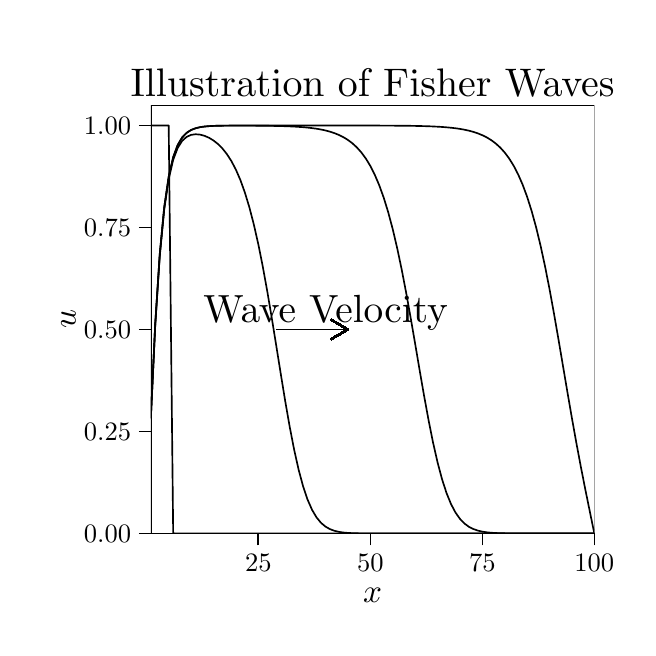
\begin{tikzpicture}[x=1pt,y=1pt]
\definecolor[named]{fillColor}{rgb}{1.00,1.00,1.00}
\path[use as bounding box,fill=fillColor,fill opacity=0.00] (0,0) rectangle (216.81,216.81);
\begin{scope}
\path[clip] (  0.00,  0.00) rectangle (216.81,216.81);
\definecolor[named]{drawColor}{rgb}{1.00,1.00,1.00}
\definecolor[named]{fillColor}{rgb}{1.00,1.00,1.00}

\path[draw=drawColor,line width= 0.6pt,line join=round,line cap=round,fill=fillColor] ( -0.00,  0.00) rectangle (216.81,216.81);
\end{scope}
\begin{scope}
\path[clip] ( 44.49, 34.03) rectangle (204.76,188.82);
\definecolor[named]{fillColor}{rgb}{1.00,1.00,1.00}

\path[fill=fillColor] ( 44.49, 34.03) rectangle (204.76,188.82);
\definecolor[named]{drawColor}{rgb}{0.00,0.00,0.00}

\path[draw=drawColor,line width= 0.6pt,line join=round] ( 44.49,181.45) --
	( 46.10,181.45) --
	( 47.72,181.45) --
	( 49.34,181.45) --
	( 50.96,181.45) --
	( 52.58, 34.03) --
	( 54.20, 34.03) --
	( 55.82, 34.03) --
	( 57.44, 34.03) --
	( 59.06, 34.03) --
	( 60.68, 34.03) --
	( 62.29, 34.03) --
	( 63.91, 34.03) --
	( 65.53, 34.03) --
	( 67.15, 34.03) --
	( 68.77, 34.03) --
	( 70.39, 34.03) --
	( 72.01, 34.03) --
	( 73.63, 34.03) --
	( 75.25, 34.03) --
	( 76.87, 34.03) --
	( 78.48, 34.03) --
	( 80.10, 34.03) --
	( 81.72, 34.03) --
	( 83.34, 34.03) --
	( 84.96, 34.03) --
	( 86.58, 34.03) --
	( 88.20, 34.03) --
	( 89.82, 34.03) --
	( 91.44, 34.03) --
	( 93.05, 34.03) --
	( 94.67, 34.03) --
	( 96.29, 34.03) --
	( 97.91, 34.03) --
	( 99.53, 34.03) --
	(101.15, 34.03) --
	(102.77, 34.03) --
	(104.39, 34.03) --
	(106.01, 34.03) --
	(107.63, 34.03) --
	(109.24, 34.03) --
	(110.86, 34.03) --
	(112.48, 34.03) --
	(114.10, 34.03) --
	(115.72, 34.03) --
	(117.34, 34.03) --
	(118.96, 34.03) --
	(120.58, 34.03) --
	(122.20, 34.03) --
	(123.82, 34.03) --
	(125.43, 34.03) --
	(127.05, 34.03) --
	(128.67, 34.03) --
	(130.29, 34.03) --
	(131.91, 34.03) --
	(133.53, 34.03) --
	(135.15, 34.03) --
	(136.77, 34.03) --
	(138.39, 34.03) --
	(140.01, 34.03) --
	(141.62, 34.03) --
	(143.24, 34.03) --
	(144.86, 34.03) --
	(146.48, 34.03) --
	(148.10, 34.03) --
	(149.72, 34.03) --
	(151.34, 34.03) --
	(152.96, 34.03) --
	(154.58, 34.03) --
	(156.20, 34.03) --
	(157.81, 34.03) --
	(159.43, 34.03) --
	(161.05, 34.03) --
	(162.67, 34.03) --
	(164.29, 34.03) --
	(165.91, 34.03) --
	(167.53, 34.03) --
	(169.15, 34.03) --
	(170.77, 34.03) --
	(172.39, 34.03) --
	(174.00, 34.03) --
	(175.62, 34.03) --
	(177.24, 34.03) --
	(178.86, 34.03) --
	(180.48, 34.03) --
	(182.10, 34.03) --
	(183.72, 34.03) --
	(185.34, 34.03) --
	(186.96, 34.03) --
	(188.58, 34.03) --
	(190.19, 34.03) --
	(191.81, 34.03) --
	(193.43, 34.03) --
	(195.05, 34.03) --
	(196.67, 34.03) --
	(198.29, 34.03) --
	(199.91, 34.03) --
	(201.53, 34.03) --
	(203.15, 34.03) --
	(204.76, 34.03);

\path[draw=drawColor,line width= 0.6pt,line join=round] ( 44.49, 75.37) --
	( 46.10,109.32) --
	( 47.72,134.15) --
	( 49.34,151.07) --
	( 50.96,162.09) --
	( 52.58,169.05) --
	( 54.20,173.34) --
	( 55.82,175.90) --
	( 57.44,177.35) --
	( 59.06,178.07) --
	( 60.68,178.30) --
	( 62.29,178.16) --
	( 63.91,177.73) --
	( 65.53,177.02) --
	( 67.15,176.04) --
	( 68.77,174.76) --
	( 70.39,173.13) --
	( 72.01,171.09) --
	( 73.63,168.57) --
	( 75.25,165.48) --
	( 76.87,161.74) --
	( 78.48,157.24) --
	( 80.10,151.92) --
	( 81.72,145.69) --
	( 83.34,138.53) --
	( 84.96,130.44) --
	( 86.58,121.52) --
	( 88.20,111.93) --
	( 89.82,101.92) --
	( 91.44, 91.80) --
	( 93.05, 81.93) --
	( 94.67, 72.66) --
	( 96.29, 64.30) --
	( 97.91, 57.07) --
	( 99.53, 51.05) --
	(101.15, 46.25) --
	(102.77, 42.56) --
	(104.39, 39.82) --
	(106.01, 37.87) --
	(107.63, 36.51) --
	(109.24, 35.60) --
	(110.86, 35.00) --
	(112.48, 34.62) --
	(114.10, 34.38) --
	(115.72, 34.24) --
	(117.34, 34.15) --
	(118.96, 34.10) --
	(120.58, 34.07) --
	(122.20, 34.05) --
	(123.82, 34.05) --
	(125.43, 34.04) --
	(127.05, 34.04) --
	(128.67, 34.04) --
	(130.29, 34.04) --
	(131.91, 34.03) --
	(133.53, 34.03) --
	(135.15, 34.03) --
	(136.77, 34.03) --
	(138.39, 34.03) --
	(140.01, 34.03) --
	(141.62, 34.03) --
	(143.24, 34.03) --
	(144.86, 34.03) --
	(146.48, 34.03) --
	(148.10, 34.03) --
	(149.72, 34.03) --
	(151.34, 34.03) --
	(152.96, 34.03) --
	(154.58, 34.03) --
	(156.20, 34.03) --
	(157.81, 34.03) --
	(159.43, 34.03) --
	(161.05, 34.03) --
	(162.67, 34.03) --
	(164.29, 34.03) --
	(165.91, 34.03) --
	(167.53, 34.03) --
	(169.15, 34.03) --
	(170.77, 34.03) --
	(172.39, 34.03) --
	(174.00, 34.03) --
	(175.62, 34.03) --
	(177.24, 34.03) --
	(178.86, 34.03) --
	(180.48, 34.03) --
	(182.10, 34.03) --
	(183.72, 34.03) --
	(185.34, 34.03) --
	(186.96, 34.03) --
	(188.58, 34.03) --
	(190.19, 34.03) --
	(191.81, 34.03) --
	(193.43, 34.03) --
	(195.05, 34.03) --
	(196.67, 34.03) --
	(198.29, 34.03) --
	(199.91, 34.03) --
	(201.53, 34.03) --
	(203.15, 34.03) --
	(204.76, 34.03);

\path[draw=drawColor,line width= 0.6pt,line join=round] ( 44.49, 75.69) --
	( 46.10,109.87) --
	( 47.72,134.84) --
	( 49.34,151.85) --
	( 50.96,162.95) --
	( 52.58,169.99) --
	( 54.20,174.40) --
	( 55.82,177.13) --
	( 57.44,178.81) --
	( 59.06,179.84) --
	( 60.68,180.46) --
	( 62.29,180.85) --
	( 63.91,181.08) --
	( 65.53,181.22) --
	( 67.15,181.31) --
	( 68.77,181.36) --
	( 70.39,181.39) --
	( 72.01,181.41) --
	( 73.63,181.42) --
	( 75.25,181.42) --
	( 76.87,181.42) --
	( 78.48,181.41) --
	( 80.10,181.41) --
	( 81.72,181.40) --
	( 83.34,181.39) --
	( 84.96,181.37) --
	( 86.58,181.35) --
	( 88.20,181.32) --
	( 89.82,181.29) --
	( 91.44,181.25) --
	( 93.05,181.20) --
	( 94.67,181.14) --
	( 96.29,181.06) --
	( 97.91,180.96) --
	( 99.53,180.85) --
	(101.15,180.70) --
	(102.77,180.51) --
	(104.39,180.29) --
	(106.01,180.01) --
	(107.63,179.66) --
	(109.24,179.23) --
	(110.86,178.70) --
	(112.48,178.04) --
	(114.10,177.23) --
	(115.72,176.24) --
	(117.34,175.02) --
	(118.96,173.53) --
	(120.58,171.71) --
	(122.20,169.51) --
	(123.82,166.84) --
	(125.43,163.64) --
	(127.05,159.83) --
	(128.67,155.33) --
	(130.29,150.08) --
	(131.91,144.01) --
	(133.53,137.11) --
	(135.15,129.41) --
	(136.77,120.99) --
	(138.39,111.98) --
	(140.01,102.60) --
	(141.62, 93.11) --
	(143.24, 83.80) --
	(144.86, 74.98) --
	(146.48, 66.90) --
	(148.10, 59.76) --
	(149.72, 53.68) --
	(151.34, 48.68) --
	(152.96, 44.69) --
	(154.58, 41.62) --
	(156.20, 39.32) --
	(157.81, 37.65) --
	(159.43, 36.46) --
	(161.05, 35.64) --
	(162.67, 35.08) --
	(164.29, 34.70) --
	(165.91, 34.46) --
	(167.53, 34.30) --
	(169.15, 34.20) --
	(170.77, 34.13) --
	(172.39, 34.09) --
	(174.00, 34.07) --
	(175.62, 34.06) --
	(177.24, 34.05) --
	(178.86, 34.04) --
	(180.48, 34.04) --
	(182.10, 34.04) --
	(183.72, 34.04) --
	(185.34, 34.04) --
	(186.96, 34.03) --
	(188.58, 34.03) --
	(190.19, 34.03) --
	(191.81, 34.03) --
	(193.43, 34.03) --
	(195.05, 34.03) --
	(196.67, 34.03) --
	(198.29, 34.03) --
	(199.91, 34.03) --
	(201.53, 34.03) --
	(203.15, 34.03) --
	(204.76, 34.03);

\path[draw=drawColor,line width= 0.6pt,line join=round] ( 44.49, 75.69) --
	( 46.10,109.87) --
	( 47.72,134.85) --
	( 49.34,151.85) --
	( 50.96,162.95) --
	( 52.58,170.00) --
	( 54.20,174.40) --
	( 55.82,177.13) --
	( 57.44,178.81) --
	( 59.06,179.84) --
	( 60.68,180.47) --
	( 62.29,180.85) --
	( 63.91,181.09) --
	( 65.53,181.23) --
	( 67.15,181.32) --
	( 68.77,181.37) --
	( 70.39,181.40) --
	( 72.01,181.42) --
	( 73.63,181.44) --
	( 75.25,181.44) --
	( 76.87,181.45) --
	( 78.48,181.45) --
	( 80.10,181.45) --
	( 81.72,181.45) --
	( 83.34,181.45) --
	( 84.96,181.45) --
	( 86.58,181.45) --
	( 88.20,181.45) --
	( 89.82,181.45) --
	( 91.44,181.45) --
	( 93.05,181.45) --
	( 94.67,181.45) --
	( 96.29,181.45) --
	( 97.91,181.45) --
	( 99.53,181.45) --
	(101.15,181.45) --
	(102.77,181.45) --
	(104.39,181.45) --
	(106.01,181.45) --
	(107.63,181.45) --
	(109.24,181.45) --
	(110.86,181.45) --
	(112.48,181.45) --
	(114.10,181.45) --
	(115.72,181.45) --
	(117.34,181.45) --
	(118.96,181.44) --
	(120.58,181.44) --
	(122.20,181.44) --
	(123.82,181.44) --
	(125.43,181.43) --
	(127.05,181.43) --
	(128.67,181.42) --
	(130.29,181.41) --
	(131.91,181.40) --
	(133.53,181.39) --
	(135.15,181.38) --
	(136.77,181.36) --
	(138.39,181.34) --
	(140.01,181.31) --
	(141.62,181.27) --
	(143.24,181.23) --
	(144.86,181.18) --
	(146.48,181.11) --
	(148.10,181.03) --
	(149.72,180.93) --
	(151.34,180.80) --
	(152.96,180.65) --
	(154.58,180.46) --
	(156.20,180.23) --
	(157.81,179.94) --
	(159.43,179.59) --
	(161.05,179.15) --
	(162.67,178.61) --
	(164.29,177.95) --
	(165.91,177.15) --
	(167.53,176.15) --
	(169.15,174.94) --
	(170.77,173.47) --
	(172.39,171.68) --
	(174.00,169.51) --
	(175.62,166.90) --
	(177.24,163.77) --
	(178.86,160.06) --
	(180.48,155.68) --
	(182.10,150.57) --
	(183.72,144.68) --
	(185.34,137.99) --
	(186.96,130.50) --
	(188.58,122.27) --
	(190.19,113.43) --
	(191.81,104.13) --
	(193.43, 94.58) --
	(195.05, 85.02) --
	(196.67, 75.65) --
	(198.29, 66.62) --
	(199.91, 58.01) --
	(201.53, 49.80) --
	(203.15, 41.86) --
	(204.76, 34.03);
\definecolor[named]{fillColor}{rgb}{0.00,0.00,0.00}

\path[draw=drawColor,line width= 0.6pt,line join=round,fill=fillColor] ( 89.82,107.74) -- (115.72,107.74);

\path[draw=drawColor,line width= 0.6pt,line join=round] (109.56,104.19) --
	(115.72,107.74) --
	(109.56,111.30);

\path[draw=drawColor,line width= 0.6pt,line join=round,fill=fillColor] ( 89.82,107.74) -- (115.72,107.74);

\path[draw=drawColor,line width= 0.6pt,line join=round] (109.56,104.19) --
	(115.72,107.74) --
	(109.56,111.30);

\path[draw=drawColor,line width= 0.6pt,line join=round,fill=fillColor] ( 89.82,107.74) -- (115.72,107.74);

\path[draw=drawColor,line width= 0.6pt,line join=round] (109.56,104.19) --
	(115.72,107.74) --
	(109.56,111.30);

\path[draw=drawColor,line width= 0.6pt,line join=round,fill=fillColor] ( 89.82,107.74) -- (115.72,107.74);

\path[draw=drawColor,line width= 0.6pt,line join=round] (109.56,104.19) --
	(115.72,107.74) --
	(109.56,111.30);

\path[draw=drawColor,line width= 0.6pt,line join=round,fill=fillColor] ( 89.82,107.74) -- (115.72,107.74);

\path[draw=drawColor,line width= 0.6pt,line join=round] (109.56,104.19) --
	(115.72,107.74) --
	(109.56,111.30);

\path[draw=drawColor,line width= 0.6pt,line join=round,fill=fillColor] ( 89.82,107.74) -- (115.72,107.74);

\path[draw=drawColor,line width= 0.6pt,line join=round] (109.56,104.19) --
	(115.72,107.74) --
	(109.56,111.30);

\path[draw=drawColor,line width= 0.6pt,line join=round,fill=fillColor] ( 89.82,107.74) -- (115.72,107.74);

\path[draw=drawColor,line width= 0.6pt,line join=round] (109.56,104.19) --
	(115.72,107.74) --
	(109.56,111.30);

\path[draw=drawColor,line width= 0.6pt,line join=round,fill=fillColor] ( 89.82,107.74) -- (115.72,107.74);

\path[draw=drawColor,line width= 0.6pt,line join=round] (109.56,104.19) --
	(115.72,107.74) --
	(109.56,111.30);

\path[draw=drawColor,line width= 0.6pt,line join=round,fill=fillColor] ( 89.82,107.74) -- (115.72,107.74);

\path[draw=drawColor,line width= 0.6pt,line join=round] (109.56,104.19) --
	(115.72,107.74) --
	(109.56,111.30);

\path[draw=drawColor,line width= 0.6pt,line join=round,fill=fillColor] ( 89.82,107.74) -- (115.72,107.74);

\path[draw=drawColor,line width= 0.6pt,line join=round] (109.56,104.19) --
	(115.72,107.74) --
	(109.56,111.30);

\path[draw=drawColor,line width= 0.6pt,line join=round,fill=fillColor] ( 89.82,107.74) -- (115.72,107.74);

\path[draw=drawColor,line width= 0.6pt,line join=round] (109.56,104.19) --
	(115.72,107.74) --
	(109.56,111.30);

\path[draw=drawColor,line width= 0.6pt,line join=round,fill=fillColor] ( 89.82,107.74) -- (115.72,107.74);

\path[draw=drawColor,line width= 0.6pt,line join=round] (109.56,104.19) --
	(115.72,107.74) --
	(109.56,111.30);

\path[draw=drawColor,line width= 0.6pt,line join=round,fill=fillColor] ( 89.82,107.74) -- (115.72,107.74);

\path[draw=drawColor,line width= 0.6pt,line join=round] (109.56,104.19) --
	(115.72,107.74) --
	(109.56,111.30);

\path[draw=drawColor,line width= 0.6pt,line join=round,fill=fillColor] ( 89.82,107.74) -- (115.72,107.74);

\path[draw=drawColor,line width= 0.6pt,line join=round] (109.56,104.19) --
	(115.72,107.74) --
	(109.56,111.30);

\path[draw=drawColor,line width= 0.6pt,line join=round,fill=fillColor] ( 89.82,107.74) -- (115.72,107.74);

\path[draw=drawColor,line width= 0.6pt,line join=round] (109.56,104.19) --
	(115.72,107.74) --
	(109.56,111.30);

\path[draw=drawColor,line width= 0.6pt,line join=round,fill=fillColor] ( 89.82,107.74) -- (115.72,107.74);

\path[draw=drawColor,line width= 0.6pt,line join=round] (109.56,104.19) --
	(115.72,107.74) --
	(109.56,111.30);

\path[draw=drawColor,line width= 0.6pt,line join=round,fill=fillColor] ( 89.82,107.74) -- (115.72,107.74);

\path[draw=drawColor,line width= 0.6pt,line join=round] (109.56,104.19) --
	(115.72,107.74) --
	(109.56,111.30);

\path[draw=drawColor,line width= 0.6pt,line join=round,fill=fillColor] ( 89.82,107.74) -- (115.72,107.74);

\path[draw=drawColor,line width= 0.6pt,line join=round] (109.56,104.19) --
	(115.72,107.74) --
	(109.56,111.30);

\path[draw=drawColor,line width= 0.6pt,line join=round,fill=fillColor] ( 89.82,107.74) -- (115.72,107.74);

\path[draw=drawColor,line width= 0.6pt,line join=round] (109.56,104.19) --
	(115.72,107.74) --
	(109.56,111.30);

\path[draw=drawColor,line width= 0.6pt,line join=round,fill=fillColor] ( 89.82,107.74) -- (115.72,107.74);

\path[draw=drawColor,line width= 0.6pt,line join=round] (109.56,104.19) --
	(115.72,107.74) --
	(109.56,111.30);

\path[draw=drawColor,line width= 0.6pt,line join=round,fill=fillColor] ( 89.82,107.74) -- (115.72,107.74);

\path[draw=drawColor,line width= 0.6pt,line join=round] (109.56,104.19) --
	(115.72,107.74) --
	(109.56,111.30);

\path[draw=drawColor,line width= 0.6pt,line join=round,fill=fillColor] ( 89.82,107.74) -- (115.72,107.74);

\path[draw=drawColor,line width= 0.6pt,line join=round] (109.56,104.19) --
	(115.72,107.74) --
	(109.56,111.30);

\path[draw=drawColor,line width= 0.6pt,line join=round,fill=fillColor] ( 89.82,107.74) -- (115.72,107.74);

\path[draw=drawColor,line width= 0.6pt,line join=round] (109.56,104.19) --
	(115.72,107.74) --
	(109.56,111.30);

\path[draw=drawColor,line width= 0.6pt,line join=round,fill=fillColor] ( 89.82,107.74) -- (115.72,107.74);

\path[draw=drawColor,line width= 0.6pt,line join=round] (109.56,104.19) --
	(115.72,107.74) --
	(109.56,111.30);

\path[draw=drawColor,line width= 0.6pt,line join=round,fill=fillColor] ( 89.82,107.74) -- (115.72,107.74);

\path[draw=drawColor,line width= 0.6pt,line join=round] (109.56,104.19) --
	(115.72,107.74) --
	(109.56,111.30);

\path[draw=drawColor,line width= 0.6pt,line join=round,fill=fillColor] ( 89.82,107.74) -- (115.72,107.74);

\path[draw=drawColor,line width= 0.6pt,line join=round] (109.56,104.19) --
	(115.72,107.74) --
	(109.56,111.30);

\path[draw=drawColor,line width= 0.6pt,line join=round,fill=fillColor] ( 89.82,107.74) -- (115.72,107.74);

\path[draw=drawColor,line width= 0.6pt,line join=round] (109.56,104.19) --
	(115.72,107.74) --
	(109.56,111.30);

\path[draw=drawColor,line width= 0.6pt,line join=round,fill=fillColor] ( 89.82,107.74) -- (115.72,107.74);

\path[draw=drawColor,line width= 0.6pt,line join=round] (109.56,104.19) --
	(115.72,107.74) --
	(109.56,111.30);

\path[draw=drawColor,line width= 0.6pt,line join=round,fill=fillColor] ( 89.82,107.74) -- (115.72,107.74);

\path[draw=drawColor,line width= 0.6pt,line join=round] (109.56,104.19) --
	(115.72,107.74) --
	(109.56,111.30);

\path[draw=drawColor,line width= 0.6pt,line join=round,fill=fillColor] ( 89.82,107.74) -- (115.72,107.74);

\path[draw=drawColor,line width= 0.6pt,line join=round] (109.56,104.19) --
	(115.72,107.74) --
	(109.56,111.30);

\path[draw=drawColor,line width= 0.6pt,line join=round,fill=fillColor] ( 89.82,107.74) -- (115.72,107.74);

\path[draw=drawColor,line width= 0.6pt,line join=round] (109.56,104.19) --
	(115.72,107.74) --
	(109.56,111.30);

\path[draw=drawColor,line width= 0.6pt,line join=round,fill=fillColor] ( 89.82,107.74) -- (115.72,107.74);

\path[draw=drawColor,line width= 0.6pt,line join=round] (109.56,104.19) --
	(115.72,107.74) --
	(109.56,111.30);

\path[draw=drawColor,line width= 0.6pt,line join=round,fill=fillColor] ( 89.82,107.74) -- (115.72,107.74);

\path[draw=drawColor,line width= 0.6pt,line join=round] (109.56,104.19) --
	(115.72,107.74) --
	(109.56,111.30);

\path[draw=drawColor,line width= 0.6pt,line join=round,fill=fillColor] ( 89.82,107.74) -- (115.72,107.74);

\path[draw=drawColor,line width= 0.6pt,line join=round] (109.56,104.19) --
	(115.72,107.74) --
	(109.56,111.30);

\path[draw=drawColor,line width= 0.6pt,line join=round,fill=fillColor] ( 89.82,107.74) -- (115.72,107.74);

\path[draw=drawColor,line width= 0.6pt,line join=round] (109.56,104.19) --
	(115.72,107.74) --
	(109.56,111.30);

\path[draw=drawColor,line width= 0.6pt,line join=round,fill=fillColor] ( 89.82,107.74) -- (115.72,107.74);

\path[draw=drawColor,line width= 0.6pt,line join=round] (109.56,104.19) --
	(115.72,107.74) --
	(109.56,111.30);

\path[draw=drawColor,line width= 0.6pt,line join=round,fill=fillColor] ( 89.82,107.74) -- (115.72,107.74);

\path[draw=drawColor,line width= 0.6pt,line join=round] (109.56,104.19) --
	(115.72,107.74) --
	(109.56,111.30);

\path[draw=drawColor,line width= 0.6pt,line join=round,fill=fillColor] ( 89.82,107.74) -- (115.72,107.74);

\path[draw=drawColor,line width= 0.6pt,line join=round] (109.56,104.19) --
	(115.72,107.74) --
	(109.56,111.30);

\path[draw=drawColor,line width= 0.6pt,line join=round,fill=fillColor] ( 89.82,107.74) -- (115.72,107.74);

\path[draw=drawColor,line width= 0.6pt,line join=round] (109.56,104.19) --
	(115.72,107.74) --
	(109.56,111.30);

\path[draw=drawColor,line width= 0.6pt,line join=round,fill=fillColor] ( 89.82,107.74) -- (115.72,107.74);

\path[draw=drawColor,line width= 0.6pt,line join=round] (109.56,104.19) --
	(115.72,107.74) --
	(109.56,111.30);

\path[draw=drawColor,line width= 0.6pt,line join=round,fill=fillColor] ( 89.82,107.74) -- (115.72,107.74);

\path[draw=drawColor,line width= 0.6pt,line join=round] (109.56,104.19) --
	(115.72,107.74) --
	(109.56,111.30);

\path[draw=drawColor,line width= 0.6pt,line join=round,fill=fillColor] ( 89.82,107.74) -- (115.72,107.74);

\path[draw=drawColor,line width= 0.6pt,line join=round] (109.56,104.19) --
	(115.72,107.74) --
	(109.56,111.30);

\path[draw=drawColor,line width= 0.6pt,line join=round,fill=fillColor] ( 89.82,107.74) -- (115.72,107.74);

\path[draw=drawColor,line width= 0.6pt,line join=round] (109.56,104.19) --
	(115.72,107.74) --
	(109.56,111.30);

\path[draw=drawColor,line width= 0.6pt,line join=round,fill=fillColor] ( 89.82,107.74) -- (115.72,107.74);

\path[draw=drawColor,line width= 0.6pt,line join=round] (109.56,104.19) --
	(115.72,107.74) --
	(109.56,111.30);

\path[draw=drawColor,line width= 0.6pt,line join=round,fill=fillColor] ( 89.82,107.74) -- (115.72,107.74);

\path[draw=drawColor,line width= 0.6pt,line join=round] (109.56,104.19) --
	(115.72,107.74) --
	(109.56,111.30);

\path[draw=drawColor,line width= 0.6pt,line join=round,fill=fillColor] ( 89.82,107.74) -- (115.72,107.74);

\path[draw=drawColor,line width= 0.6pt,line join=round] (109.56,104.19) --
	(115.72,107.74) --
	(109.56,111.30);

\path[draw=drawColor,line width= 0.6pt,line join=round,fill=fillColor] ( 89.82,107.74) -- (115.72,107.74);

\path[draw=drawColor,line width= 0.6pt,line join=round] (109.56,104.19) --
	(115.72,107.74) --
	(109.56,111.30);

\path[draw=drawColor,line width= 0.6pt,line join=round,fill=fillColor] ( 89.82,107.74) -- (115.72,107.74);

\path[draw=drawColor,line width= 0.6pt,line join=round] (109.56,104.19) --
	(115.72,107.74) --
	(109.56,111.30);

\path[draw=drawColor,line width= 0.6pt,line join=round,fill=fillColor] ( 89.82,107.74) -- (115.72,107.74);

\path[draw=drawColor,line width= 0.6pt,line join=round] (109.56,104.19) --
	(115.72,107.74) --
	(109.56,111.30);

\path[draw=drawColor,line width= 0.6pt,line join=round,fill=fillColor] ( 89.82,107.74) -- (115.72,107.74);

\path[draw=drawColor,line width= 0.6pt,line join=round] (109.56,104.19) --
	(115.72,107.74) --
	(109.56,111.30);

\path[draw=drawColor,line width= 0.6pt,line join=round,fill=fillColor] ( 89.82,107.74) -- (115.72,107.74);

\path[draw=drawColor,line width= 0.6pt,line join=round] (109.56,104.19) --
	(115.72,107.74) --
	(109.56,111.30);

\path[draw=drawColor,line width= 0.6pt,line join=round,fill=fillColor] ( 89.82,107.74) -- (115.72,107.74);

\path[draw=drawColor,line width= 0.6pt,line join=round] (109.56,104.19) --
	(115.72,107.74) --
	(109.56,111.30);

\path[draw=drawColor,line width= 0.6pt,line join=round,fill=fillColor] ( 89.82,107.74) -- (115.72,107.74);

\path[draw=drawColor,line width= 0.6pt,line join=round] (109.56,104.19) --
	(115.72,107.74) --
	(109.56,111.30);

\path[draw=drawColor,line width= 0.6pt,line join=round,fill=fillColor] ( 89.82,107.74) -- (115.72,107.74);

\path[draw=drawColor,line width= 0.6pt,line join=round] (109.56,104.19) --
	(115.72,107.74) --
	(109.56,111.30);

\path[draw=drawColor,line width= 0.6pt,line join=round,fill=fillColor] ( 89.82,107.74) -- (115.72,107.74);

\path[draw=drawColor,line width= 0.6pt,line join=round] (109.56,104.19) --
	(115.72,107.74) --
	(109.56,111.30);

\path[draw=drawColor,line width= 0.6pt,line join=round,fill=fillColor] ( 89.82,107.74) -- (115.72,107.74);

\path[draw=drawColor,line width= 0.6pt,line join=round] (109.56,104.19) --
	(115.72,107.74) --
	(109.56,111.30);

\path[draw=drawColor,line width= 0.6pt,line join=round,fill=fillColor] ( 89.82,107.74) -- (115.72,107.74);

\path[draw=drawColor,line width= 0.6pt,line join=round] (109.56,104.19) --
	(115.72,107.74) --
	(109.56,111.30);

\path[draw=drawColor,line width= 0.6pt,line join=round,fill=fillColor] ( 89.82,107.74) -- (115.72,107.74);

\path[draw=drawColor,line width= 0.6pt,line join=round] (109.56,104.19) --
	(115.72,107.74) --
	(109.56,111.30);

\path[draw=drawColor,line width= 0.6pt,line join=round,fill=fillColor] ( 89.82,107.74) -- (115.72,107.74);

\path[draw=drawColor,line width= 0.6pt,line join=round] (109.56,104.19) --
	(115.72,107.74) --
	(109.56,111.30);

\path[draw=drawColor,line width= 0.6pt,line join=round,fill=fillColor] ( 89.82,107.74) -- (115.72,107.74);

\path[draw=drawColor,line width= 0.6pt,line join=round] (109.56,104.19) --
	(115.72,107.74) --
	(109.56,111.30);

\path[draw=drawColor,line width= 0.6pt,line join=round,fill=fillColor] ( 89.82,107.74) -- (115.72,107.74);

\path[draw=drawColor,line width= 0.6pt,line join=round] (109.56,104.19) --
	(115.72,107.74) --
	(109.56,111.30);

\path[draw=drawColor,line width= 0.6pt,line join=round,fill=fillColor] ( 89.82,107.74) -- (115.72,107.74);

\path[draw=drawColor,line width= 0.6pt,line join=round] (109.56,104.19) --
	(115.72,107.74) --
	(109.56,111.30);

\path[draw=drawColor,line width= 0.6pt,line join=round,fill=fillColor] ( 89.82,107.74) -- (115.72,107.74);

\path[draw=drawColor,line width= 0.6pt,line join=round] (109.56,104.19) --
	(115.72,107.74) --
	(109.56,111.30);

\path[draw=drawColor,line width= 0.6pt,line join=round,fill=fillColor] ( 89.82,107.74) -- (115.72,107.74);

\path[draw=drawColor,line width= 0.6pt,line join=round] (109.56,104.19) --
	(115.72,107.74) --
	(109.56,111.30);

\path[draw=drawColor,line width= 0.6pt,line join=round,fill=fillColor] ( 89.82,107.74) -- (115.72,107.74);

\path[draw=drawColor,line width= 0.6pt,line join=round] (109.56,104.19) --
	(115.72,107.74) --
	(109.56,111.30);

\path[draw=drawColor,line width= 0.6pt,line join=round,fill=fillColor] ( 89.82,107.74) -- (115.72,107.74);

\path[draw=drawColor,line width= 0.6pt,line join=round] (109.56,104.19) --
	(115.72,107.74) --
	(109.56,111.30);

\path[draw=drawColor,line width= 0.6pt,line join=round,fill=fillColor] ( 89.82,107.74) -- (115.72,107.74);

\path[draw=drawColor,line width= 0.6pt,line join=round] (109.56,104.19) --
	(115.72,107.74) --
	(109.56,111.30);

\path[draw=drawColor,line width= 0.6pt,line join=round,fill=fillColor] ( 89.82,107.74) -- (115.72,107.74);

\path[draw=drawColor,line width= 0.6pt,line join=round] (109.56,104.19) --
	(115.72,107.74) --
	(109.56,111.30);

\path[draw=drawColor,line width= 0.6pt,line join=round,fill=fillColor] ( 89.82,107.74) -- (115.72,107.74);

\path[draw=drawColor,line width= 0.6pt,line join=round] (109.56,104.19) --
	(115.72,107.74) --
	(109.56,111.30);

\path[draw=drawColor,line width= 0.6pt,line join=round,fill=fillColor] ( 89.82,107.74) -- (115.72,107.74);

\path[draw=drawColor,line width= 0.6pt,line join=round] (109.56,104.19) --
	(115.72,107.74) --
	(109.56,111.30);

\path[draw=drawColor,line width= 0.6pt,line join=round,fill=fillColor] ( 89.82,107.74) -- (115.72,107.74);

\path[draw=drawColor,line width= 0.6pt,line join=round] (109.56,104.19) --
	(115.72,107.74) --
	(109.56,111.30);

\path[draw=drawColor,line width= 0.6pt,line join=round,fill=fillColor] ( 89.82,107.74) -- (115.72,107.74);

\path[draw=drawColor,line width= 0.6pt,line join=round] (109.56,104.19) --
	(115.72,107.74) --
	(109.56,111.30);

\path[draw=drawColor,line width= 0.6pt,line join=round,fill=fillColor] ( 89.82,107.74) -- (115.72,107.74);

\path[draw=drawColor,line width= 0.6pt,line join=round] (109.56,104.19) --
	(115.72,107.74) --
	(109.56,111.30);

\path[draw=drawColor,line width= 0.6pt,line join=round,fill=fillColor] ( 89.82,107.74) -- (115.72,107.74);

\path[draw=drawColor,line width= 0.6pt,line join=round] (109.56,104.19) --
	(115.72,107.74) --
	(109.56,111.30);

\path[draw=drawColor,line width= 0.6pt,line join=round,fill=fillColor] ( 89.82,107.74) -- (115.72,107.74);

\path[draw=drawColor,line width= 0.6pt,line join=round] (109.56,104.19) --
	(115.72,107.74) --
	(109.56,111.30);

\path[draw=drawColor,line width= 0.6pt,line join=round,fill=fillColor] ( 89.82,107.74) -- (115.72,107.74);

\path[draw=drawColor,line width= 0.6pt,line join=round] (109.56,104.19) --
	(115.72,107.74) --
	(109.56,111.30);

\path[draw=drawColor,line width= 0.6pt,line join=round,fill=fillColor] ( 89.82,107.74) -- (115.72,107.74);

\path[draw=drawColor,line width= 0.6pt,line join=round] (109.56,104.19) --
	(115.72,107.74) --
	(109.56,111.30);

\path[draw=drawColor,line width= 0.6pt,line join=round,fill=fillColor] ( 89.82,107.74) -- (115.72,107.74);

\path[draw=drawColor,line width= 0.6pt,line join=round] (109.56,104.19) --
	(115.72,107.74) --
	(109.56,111.30);

\path[draw=drawColor,line width= 0.6pt,line join=round,fill=fillColor] ( 89.82,107.74) -- (115.72,107.74);

\path[draw=drawColor,line width= 0.6pt,line join=round] (109.56,104.19) --
	(115.72,107.74) --
	(109.56,111.30);

\path[draw=drawColor,line width= 0.6pt,line join=round,fill=fillColor] ( 89.82,107.74) -- (115.72,107.74);

\path[draw=drawColor,line width= 0.6pt,line join=round] (109.56,104.19) --
	(115.72,107.74) --
	(109.56,111.30);

\path[draw=drawColor,line width= 0.6pt,line join=round,fill=fillColor] ( 89.82,107.74) -- (115.72,107.74);

\path[draw=drawColor,line width= 0.6pt,line join=round] (109.56,104.19) --
	(115.72,107.74) --
	(109.56,111.30);

\path[draw=drawColor,line width= 0.6pt,line join=round,fill=fillColor] ( 89.82,107.74) -- (115.72,107.74);

\path[draw=drawColor,line width= 0.6pt,line join=round] (109.56,104.19) --
	(115.72,107.74) --
	(109.56,111.30);

\path[draw=drawColor,line width= 0.6pt,line join=round,fill=fillColor] ( 89.82,107.74) -- (115.72,107.74);

\path[draw=drawColor,line width= 0.6pt,line join=round] (109.56,104.19) --
	(115.72,107.74) --
	(109.56,111.30);

\path[draw=drawColor,line width= 0.6pt,line join=round,fill=fillColor] ( 89.82,107.74) -- (115.72,107.74);

\path[draw=drawColor,line width= 0.6pt,line join=round] (109.56,104.19) --
	(115.72,107.74) --
	(109.56,111.30);

\path[draw=drawColor,line width= 0.6pt,line join=round,fill=fillColor] ( 89.82,107.74) -- (115.72,107.74);

\path[draw=drawColor,line width= 0.6pt,line join=round] (109.56,104.19) --
	(115.72,107.74) --
	(109.56,111.30);

\path[draw=drawColor,line width= 0.6pt,line join=round,fill=fillColor] ( 89.82,107.74) -- (115.72,107.74);

\path[draw=drawColor,line width= 0.6pt,line join=round] (109.56,104.19) --
	(115.72,107.74) --
	(109.56,111.30);

\path[draw=drawColor,line width= 0.6pt,line join=round,fill=fillColor] ( 89.82,107.74) -- (115.72,107.74);

\path[draw=drawColor,line width= 0.6pt,line join=round] (109.56,104.19) --
	(115.72,107.74) --
	(109.56,111.30);

\path[draw=drawColor,line width= 0.6pt,line join=round,fill=fillColor] ( 89.82,107.74) -- (115.72,107.74);

\path[draw=drawColor,line width= 0.6pt,line join=round] (109.56,104.19) --
	(115.72,107.74) --
	(109.56,111.30);

\path[draw=drawColor,line width= 0.6pt,line join=round,fill=fillColor] ( 89.82,107.74) -- (115.72,107.74);

\path[draw=drawColor,line width= 0.6pt,line join=round] (109.56,104.19) --
	(115.72,107.74) --
	(109.56,111.30);

\path[draw=drawColor,line width= 0.6pt,line join=round,fill=fillColor] ( 89.82,107.74) -- (115.72,107.74);

\path[draw=drawColor,line width= 0.6pt,line join=round] (109.56,104.19) --
	(115.72,107.74) --
	(109.56,111.30);

\path[draw=drawColor,line width= 0.6pt,line join=round,fill=fillColor] ( 89.82,107.74) -- (115.72,107.74);

\path[draw=drawColor,line width= 0.6pt,line join=round] (109.56,104.19) --
	(115.72,107.74) --
	(109.56,111.30);

\path[draw=drawColor,line width= 0.6pt,line join=round,fill=fillColor] ( 89.82,107.74) -- (115.72,107.74);

\path[draw=drawColor,line width= 0.6pt,line join=round] (109.56,104.19) --
	(115.72,107.74) --
	(109.56,111.30);

\path[draw=drawColor,line width= 0.6pt,line join=round,fill=fillColor] ( 89.82,107.74) -- (115.72,107.74);

\path[draw=drawColor,line width= 0.6pt,line join=round] (109.56,104.19) --
	(115.72,107.74) --
	(109.56,111.30);

\path[draw=drawColor,line width= 0.6pt,line join=round,fill=fillColor] ( 89.82,107.74) -- (115.72,107.74);

\path[draw=drawColor,line width= 0.6pt,line join=round] (109.56,104.19) --
	(115.72,107.74) --
	(109.56,111.30);

\path[draw=drawColor,line width= 0.6pt,line join=round,fill=fillColor] ( 89.82,107.74) -- (115.72,107.74);

\path[draw=drawColor,line width= 0.6pt,line join=round] (109.56,104.19) --
	(115.72,107.74) --
	(109.56,111.30);

\path[draw=drawColor,line width= 0.6pt,line join=round,fill=fillColor] ( 89.82,107.74) -- (115.72,107.74);

\path[draw=drawColor,line width= 0.6pt,line join=round] (109.56,104.19) --
	(115.72,107.74) --
	(109.56,111.30);

\path[draw=drawColor,line width= 0.6pt,line join=round,fill=fillColor] ( 89.82,107.74) -- (115.72,107.74);

\path[draw=drawColor,line width= 0.6pt,line join=round] (109.56,104.19) --
	(115.72,107.74) --
	(109.56,111.30);

\path[draw=drawColor,line width= 0.6pt,line join=round,fill=fillColor] ( 89.82,107.74) -- (115.72,107.74);

\path[draw=drawColor,line width= 0.6pt,line join=round] (109.56,104.19) --
	(115.72,107.74) --
	(109.56,111.30);

\path[draw=drawColor,line width= 0.6pt,line join=round,fill=fillColor] ( 89.82,107.74) -- (115.72,107.74);

\path[draw=drawColor,line width= 0.6pt,line join=round] (109.56,104.19) --
	(115.72,107.74) --
	(109.56,111.30);

\path[draw=drawColor,line width= 0.6pt,line join=round,fill=fillColor] ( 89.82,107.74) -- (115.72,107.74);

\path[draw=drawColor,line width= 0.6pt,line join=round] (109.56,104.19) --
	(115.72,107.74) --
	(109.56,111.30);

\path[draw=drawColor,line width= 0.6pt,line join=round,fill=fillColor] ( 89.82,107.74) -- (115.72,107.74);

\path[draw=drawColor,line width= 0.6pt,line join=round] (109.56,104.19) --
	(115.72,107.74) --
	(109.56,111.30);

\path[draw=drawColor,line width= 0.6pt,line join=round,fill=fillColor] ( 89.82,107.74) -- (115.72,107.74);

\path[draw=drawColor,line width= 0.6pt,line join=round] (109.56,104.19) --
	(115.72,107.74) --
	(109.56,111.30);

\path[draw=drawColor,line width= 0.6pt,line join=round,fill=fillColor] ( 89.82,107.74) -- (115.72,107.74);

\path[draw=drawColor,line width= 0.6pt,line join=round] (109.56,104.19) --
	(115.72,107.74) --
	(109.56,111.30);

\path[draw=drawColor,line width= 0.6pt,line join=round,fill=fillColor] ( 89.82,107.74) -- (115.72,107.74);

\path[draw=drawColor,line width= 0.6pt,line join=round] (109.56,104.19) --
	(115.72,107.74) --
	(109.56,111.30);

\path[draw=drawColor,line width= 0.6pt,line join=round,fill=fillColor] ( 89.82,107.74) -- (115.72,107.74);

\path[draw=drawColor,line width= 0.6pt,line join=round] (109.56,104.19) --
	(115.72,107.74) --
	(109.56,111.30);

\path[draw=drawColor,line width= 0.6pt,line join=round,fill=fillColor] ( 89.82,107.74) -- (115.72,107.74);

\path[draw=drawColor,line width= 0.6pt,line join=round] (109.56,104.19) --
	(115.72,107.74) --
	(109.56,111.30);

\path[draw=drawColor,line width= 0.6pt,line join=round,fill=fillColor] ( 89.82,107.74) -- (115.72,107.74);

\path[draw=drawColor,line width= 0.6pt,line join=round] (109.56,104.19) --
	(115.72,107.74) --
	(109.56,111.30);

\path[draw=drawColor,line width= 0.6pt,line join=round,fill=fillColor] ( 89.82,107.74) -- (115.72,107.74);

\path[draw=drawColor,line width= 0.6pt,line join=round] (109.56,104.19) --
	(115.72,107.74) --
	(109.56,111.30);

\path[draw=drawColor,line width= 0.6pt,line join=round,fill=fillColor] ( 89.82,107.74) -- (115.72,107.74);

\path[draw=drawColor,line width= 0.6pt,line join=round] (109.56,104.19) --
	(115.72,107.74) --
	(109.56,111.30);

\path[draw=drawColor,line width= 0.6pt,line join=round,fill=fillColor] ( 89.82,107.74) -- (115.72,107.74);

\path[draw=drawColor,line width= 0.6pt,line join=round] (109.56,104.19) --
	(115.72,107.74) --
	(109.56,111.30);

\path[draw=drawColor,line width= 0.6pt,line join=round,fill=fillColor] ( 89.82,107.74) -- (115.72,107.74);

\path[draw=drawColor,line width= 0.6pt,line join=round] (109.56,104.19) --
	(115.72,107.74) --
	(109.56,111.30);

\path[draw=drawColor,line width= 0.6pt,line join=round,fill=fillColor] ( 89.82,107.74) -- (115.72,107.74);

\path[draw=drawColor,line width= 0.6pt,line join=round] (109.56,104.19) --
	(115.72,107.74) --
	(109.56,111.30);

\path[draw=drawColor,line width= 0.6pt,line join=round,fill=fillColor] ( 89.82,107.74) -- (115.72,107.74);

\path[draw=drawColor,line width= 0.6pt,line join=round] (109.56,104.19) --
	(115.72,107.74) --
	(109.56,111.30);

\path[draw=drawColor,line width= 0.6pt,line join=round,fill=fillColor] ( 89.82,107.74) -- (115.72,107.74);

\path[draw=drawColor,line width= 0.6pt,line join=round] (109.56,104.19) --
	(115.72,107.74) --
	(109.56,111.30);

\path[draw=drawColor,line width= 0.6pt,line join=round,fill=fillColor] ( 89.82,107.74) -- (115.72,107.74);

\path[draw=drawColor,line width= 0.6pt,line join=round] (109.56,104.19) --
	(115.72,107.74) --
	(109.56,111.30);

\path[draw=drawColor,line width= 0.6pt,line join=round,fill=fillColor] ( 89.82,107.74) -- (115.72,107.74);

\path[draw=drawColor,line width= 0.6pt,line join=round] (109.56,104.19) --
	(115.72,107.74) --
	(109.56,111.30);

\path[draw=drawColor,line width= 0.6pt,line join=round,fill=fillColor] ( 89.82,107.74) -- (115.72,107.74);

\path[draw=drawColor,line width= 0.6pt,line join=round] (109.56,104.19) --
	(115.72,107.74) --
	(109.56,111.30);

\path[draw=drawColor,line width= 0.6pt,line join=round,fill=fillColor] ( 89.82,107.74) -- (115.72,107.74);

\path[draw=drawColor,line width= 0.6pt,line join=round] (109.56,104.19) --
	(115.72,107.74) --
	(109.56,111.30);

\path[draw=drawColor,line width= 0.6pt,line join=round,fill=fillColor] ( 89.82,107.74) -- (115.72,107.74);

\path[draw=drawColor,line width= 0.6pt,line join=round] (109.56,104.19) --
	(115.72,107.74) --
	(109.56,111.30);

\path[draw=drawColor,line width= 0.6pt,line join=round,fill=fillColor] ( 89.82,107.74) -- (115.72,107.74);

\path[draw=drawColor,line width= 0.6pt,line join=round] (109.56,104.19) --
	(115.72,107.74) --
	(109.56,111.30);

\path[draw=drawColor,line width= 0.6pt,line join=round,fill=fillColor] ( 89.82,107.74) -- (115.72,107.74);

\path[draw=drawColor,line width= 0.6pt,line join=round] (109.56,104.19) --
	(115.72,107.74) --
	(109.56,111.30);

\path[draw=drawColor,line width= 0.6pt,line join=round,fill=fillColor] ( 89.82,107.74) -- (115.72,107.74);

\path[draw=drawColor,line width= 0.6pt,line join=round] (109.56,104.19) --
	(115.72,107.74) --
	(109.56,111.30);

\path[draw=drawColor,line width= 0.6pt,line join=round,fill=fillColor] ( 89.82,107.74) -- (115.72,107.74);

\path[draw=drawColor,line width= 0.6pt,line join=round] (109.56,104.19) --
	(115.72,107.74) --
	(109.56,111.30);

\path[draw=drawColor,line width= 0.6pt,line join=round,fill=fillColor] ( 89.82,107.74) -- (115.72,107.74);

\path[draw=drawColor,line width= 0.6pt,line join=round] (109.56,104.19) --
	(115.72,107.74) --
	(109.56,111.30);

\path[draw=drawColor,line width= 0.6pt,line join=round,fill=fillColor] ( 89.82,107.74) -- (115.72,107.74);

\path[draw=drawColor,line width= 0.6pt,line join=round] (109.56,104.19) --
	(115.72,107.74) --
	(109.56,111.30);

\path[draw=drawColor,line width= 0.6pt,line join=round,fill=fillColor] ( 89.82,107.74) -- (115.72,107.74);

\path[draw=drawColor,line width= 0.6pt,line join=round] (109.56,104.19) --
	(115.72,107.74) --
	(109.56,111.30);

\path[draw=drawColor,line width= 0.6pt,line join=round,fill=fillColor] ( 89.82,107.74) -- (115.72,107.74);

\path[draw=drawColor,line width= 0.6pt,line join=round] (109.56,104.19) --
	(115.72,107.74) --
	(109.56,111.30);

\path[draw=drawColor,line width= 0.6pt,line join=round,fill=fillColor] ( 89.82,107.74) -- (115.72,107.74);

\path[draw=drawColor,line width= 0.6pt,line join=round] (109.56,104.19) --
	(115.72,107.74) --
	(109.56,111.30);

\path[draw=drawColor,line width= 0.6pt,line join=round,fill=fillColor] ( 89.82,107.74) -- (115.72,107.74);

\path[draw=drawColor,line width= 0.6pt,line join=round] (109.56,104.19) --
	(115.72,107.74) --
	(109.56,111.30);

\path[draw=drawColor,line width= 0.6pt,line join=round,fill=fillColor] ( 89.82,107.74) -- (115.72,107.74);

\path[draw=drawColor,line width= 0.6pt,line join=round] (109.56,104.19) --
	(115.72,107.74) --
	(109.56,111.30);

\path[draw=drawColor,line width= 0.6pt,line join=round,fill=fillColor] ( 89.82,107.74) -- (115.72,107.74);

\path[draw=drawColor,line width= 0.6pt,line join=round] (109.56,104.19) --
	(115.72,107.74) --
	(109.56,111.30);

\path[draw=drawColor,line width= 0.6pt,line join=round,fill=fillColor] ( 89.82,107.74) -- (115.72,107.74);

\path[draw=drawColor,line width= 0.6pt,line join=round] (109.56,104.19) --
	(115.72,107.74) --
	(109.56,111.30);

\path[draw=drawColor,line width= 0.6pt,line join=round,fill=fillColor] ( 89.82,107.74) -- (115.72,107.74);

\path[draw=drawColor,line width= 0.6pt,line join=round] (109.56,104.19) --
	(115.72,107.74) --
	(109.56,111.30);

\path[draw=drawColor,line width= 0.6pt,line join=round,fill=fillColor] ( 89.82,107.74) -- (115.72,107.74);

\path[draw=drawColor,line width= 0.6pt,line join=round] (109.56,104.19) --
	(115.72,107.74) --
	(109.56,111.30);

\path[draw=drawColor,line width= 0.6pt,line join=round,fill=fillColor] ( 89.82,107.74) -- (115.72,107.74);

\path[draw=drawColor,line width= 0.6pt,line join=round] (109.56,104.19) --
	(115.72,107.74) --
	(109.56,111.30);

\path[draw=drawColor,line width= 0.6pt,line join=round,fill=fillColor] ( 89.82,107.74) -- (115.72,107.74);

\path[draw=drawColor,line width= 0.6pt,line join=round] (109.56,104.19) --
	(115.72,107.74) --
	(109.56,111.30);

\path[draw=drawColor,line width= 0.6pt,line join=round,fill=fillColor] ( 89.82,107.74) -- (115.72,107.74);

\path[draw=drawColor,line width= 0.6pt,line join=round] (109.56,104.19) --
	(115.72,107.74) --
	(109.56,111.30);

\path[draw=drawColor,line width= 0.6pt,line join=round,fill=fillColor] ( 89.82,107.74) -- (115.72,107.74);

\path[draw=drawColor,line width= 0.6pt,line join=round] (109.56,104.19) --
	(115.72,107.74) --
	(109.56,111.30);

\path[draw=drawColor,line width= 0.6pt,line join=round,fill=fillColor] ( 89.82,107.74) -- (115.72,107.74);

\path[draw=drawColor,line width= 0.6pt,line join=round] (109.56,104.19) --
	(115.72,107.74) --
	(109.56,111.30);

\path[draw=drawColor,line width= 0.6pt,line join=round,fill=fillColor] ( 89.82,107.74) -- (115.72,107.74);

\path[draw=drawColor,line width= 0.6pt,line join=round] (109.56,104.19) --
	(115.72,107.74) --
	(109.56,111.30);

\path[draw=drawColor,line width= 0.6pt,line join=round,fill=fillColor] ( 89.82,107.74) -- (115.72,107.74);

\path[draw=drawColor,line width= 0.6pt,line join=round] (109.56,104.19) --
	(115.72,107.74) --
	(109.56,111.30);

\path[draw=drawColor,line width= 0.6pt,line join=round,fill=fillColor] ( 89.82,107.74) -- (115.72,107.74);

\path[draw=drawColor,line width= 0.6pt,line join=round] (109.56,104.19) --
	(115.72,107.74) --
	(109.56,111.30);

\path[draw=drawColor,line width= 0.6pt,line join=round,fill=fillColor] ( 89.82,107.74) -- (115.72,107.74);

\path[draw=drawColor,line width= 0.6pt,line join=round] (109.56,104.19) --
	(115.72,107.74) --
	(109.56,111.30);

\path[draw=drawColor,line width= 0.6pt,line join=round,fill=fillColor] ( 89.82,107.74) -- (115.72,107.74);

\path[draw=drawColor,line width= 0.6pt,line join=round] (109.56,104.19) --
	(115.72,107.74) --
	(109.56,111.30);

\path[draw=drawColor,line width= 0.6pt,line join=round,fill=fillColor] ( 89.82,107.74) -- (115.72,107.74);

\path[draw=drawColor,line width= 0.6pt,line join=round] (109.56,104.19) --
	(115.72,107.74) --
	(109.56,111.30);

\path[draw=drawColor,line width= 0.6pt,line join=round,fill=fillColor] ( 89.82,107.74) -- (115.72,107.74);

\path[draw=drawColor,line width= 0.6pt,line join=round] (109.56,104.19) --
	(115.72,107.74) --
	(109.56,111.30);

\path[draw=drawColor,line width= 0.6pt,line join=round,fill=fillColor] ( 89.82,107.74) -- (115.72,107.74);

\path[draw=drawColor,line width= 0.6pt,line join=round] (109.56,104.19) --
	(115.72,107.74) --
	(109.56,111.30);

\path[draw=drawColor,line width= 0.6pt,line join=round,fill=fillColor] ( 89.82,107.74) -- (115.72,107.74);

\path[draw=drawColor,line width= 0.6pt,line join=round] (109.56,104.19) --
	(115.72,107.74) --
	(109.56,111.30);

\path[draw=drawColor,line width= 0.6pt,line join=round,fill=fillColor] ( 89.82,107.74) -- (115.72,107.74);

\path[draw=drawColor,line width= 0.6pt,line join=round] (109.56,104.19) --
	(115.72,107.74) --
	(109.56,111.30);

\path[draw=drawColor,line width= 0.6pt,line join=round,fill=fillColor] ( 89.82,107.74) -- (115.72,107.74);

\path[draw=drawColor,line width= 0.6pt,line join=round] (109.56,104.19) --
	(115.72,107.74) --
	(109.56,111.30);

\path[draw=drawColor,line width= 0.6pt,line join=round,fill=fillColor] ( 89.82,107.74) -- (115.72,107.74);

\path[draw=drawColor,line width= 0.6pt,line join=round] (109.56,104.19) --
	(115.72,107.74) --
	(109.56,111.30);

\path[draw=drawColor,line width= 0.6pt,line join=round,fill=fillColor] ( 89.82,107.74) -- (115.72,107.74);

\path[draw=drawColor,line width= 0.6pt,line join=round] (109.56,104.19) --
	(115.72,107.74) --
	(109.56,111.30);

\path[draw=drawColor,line width= 0.6pt,line join=round,fill=fillColor] ( 89.82,107.74) -- (115.72,107.74);

\path[draw=drawColor,line width= 0.6pt,line join=round] (109.56,104.19) --
	(115.72,107.74) --
	(109.56,111.30);

\path[draw=drawColor,line width= 0.6pt,line join=round,fill=fillColor] ( 89.82,107.74) -- (115.72,107.74);

\path[draw=drawColor,line width= 0.6pt,line join=round] (109.56,104.19) --
	(115.72,107.74) --
	(109.56,111.30);

\path[draw=drawColor,line width= 0.6pt,line join=round,fill=fillColor] ( 89.82,107.74) -- (115.72,107.74);

\path[draw=drawColor,line width= 0.6pt,line join=round] (109.56,104.19) --
	(115.72,107.74) --
	(109.56,111.30);

\path[draw=drawColor,line width= 0.6pt,line join=round,fill=fillColor] ( 89.82,107.74) -- (115.72,107.74);

\path[draw=drawColor,line width= 0.6pt,line join=round] (109.56,104.19) --
	(115.72,107.74) --
	(109.56,111.30);

\path[draw=drawColor,line width= 0.6pt,line join=round,fill=fillColor] ( 89.82,107.74) -- (115.72,107.74);

\path[draw=drawColor,line width= 0.6pt,line join=round] (109.56,104.19) --
	(115.72,107.74) --
	(109.56,111.30);

\path[draw=drawColor,line width= 0.6pt,line join=round,fill=fillColor] ( 89.82,107.74) -- (115.72,107.74);

\path[draw=drawColor,line width= 0.6pt,line join=round] (109.56,104.19) --
	(115.72,107.74) --
	(109.56,111.30);

\path[draw=drawColor,line width= 0.6pt,line join=round,fill=fillColor] ( 89.82,107.74) -- (115.72,107.74);

\path[draw=drawColor,line width= 0.6pt,line join=round] (109.56,104.19) --
	(115.72,107.74) --
	(109.56,111.30);

\path[draw=drawColor,line width= 0.6pt,line join=round,fill=fillColor] ( 89.82,107.74) -- (115.72,107.74);

\path[draw=drawColor,line width= 0.6pt,line join=round] (109.56,104.19) --
	(115.72,107.74) --
	(109.56,111.30);

\path[draw=drawColor,line width= 0.6pt,line join=round,fill=fillColor] ( 89.82,107.74) -- (115.72,107.74);

\path[draw=drawColor,line width= 0.6pt,line join=round] (109.56,104.19) --
	(115.72,107.74) --
	(109.56,111.30);

\path[draw=drawColor,line width= 0.6pt,line join=round,fill=fillColor] ( 89.82,107.74) -- (115.72,107.74);

\path[draw=drawColor,line width= 0.6pt,line join=round] (109.56,104.19) --
	(115.72,107.74) --
	(109.56,111.30);

\path[draw=drawColor,line width= 0.6pt,line join=round,fill=fillColor] ( 89.82,107.74) -- (115.72,107.74);

\path[draw=drawColor,line width= 0.6pt,line join=round] (109.56,104.19) --
	(115.72,107.74) --
	(109.56,111.30);

\path[draw=drawColor,line width= 0.6pt,line join=round,fill=fillColor] ( 89.82,107.74) -- (115.72,107.74);

\path[draw=drawColor,line width= 0.6pt,line join=round] (109.56,104.19) --
	(115.72,107.74) --
	(109.56,111.30);

\path[draw=drawColor,line width= 0.6pt,line join=round,fill=fillColor] ( 89.82,107.74) -- (115.72,107.74);

\path[draw=drawColor,line width= 0.6pt,line join=round] (109.56,104.19) --
	(115.72,107.74) --
	(109.56,111.30);

\path[draw=drawColor,line width= 0.6pt,line join=round,fill=fillColor] ( 89.82,107.74) -- (115.72,107.74);

\path[draw=drawColor,line width= 0.6pt,line join=round] (109.56,104.19) --
	(115.72,107.74) --
	(109.56,111.30);

\path[draw=drawColor,line width= 0.6pt,line join=round,fill=fillColor] ( 89.82,107.74) -- (115.72,107.74);

\path[draw=drawColor,line width= 0.6pt,line join=round] (109.56,104.19) --
	(115.72,107.74) --
	(109.56,111.30);

\path[draw=drawColor,line width= 0.6pt,line join=round,fill=fillColor] ( 89.82,107.74) -- (115.72,107.74);

\path[draw=drawColor,line width= 0.6pt,line join=round] (109.56,104.19) --
	(115.72,107.74) --
	(109.56,111.30);

\path[draw=drawColor,line width= 0.6pt,line join=round,fill=fillColor] ( 89.82,107.74) -- (115.72,107.74);

\path[draw=drawColor,line width= 0.6pt,line join=round] (109.56,104.19) --
	(115.72,107.74) --
	(109.56,111.30);

\path[draw=drawColor,line width= 0.6pt,line join=round,fill=fillColor] ( 89.82,107.74) -- (115.72,107.74);

\path[draw=drawColor,line width= 0.6pt,line join=round] (109.56,104.19) --
	(115.72,107.74) --
	(109.56,111.30);

\path[draw=drawColor,line width= 0.6pt,line join=round,fill=fillColor] ( 89.82,107.74) -- (115.72,107.74);

\path[draw=drawColor,line width= 0.6pt,line join=round] (109.56,104.19) --
	(115.72,107.74) --
	(109.56,111.30);

\path[draw=drawColor,line width= 0.6pt,line join=round,fill=fillColor] ( 89.82,107.74) -- (115.72,107.74);

\path[draw=drawColor,line width= 0.6pt,line join=round] (109.56,104.19) --
	(115.72,107.74) --
	(109.56,111.30);

\path[draw=drawColor,line width= 0.6pt,line join=round,fill=fillColor] ( 89.82,107.74) -- (115.72,107.74);

\path[draw=drawColor,line width= 0.6pt,line join=round] (109.56,104.19) --
	(115.72,107.74) --
	(109.56,111.30);

\path[draw=drawColor,line width= 0.6pt,line join=round,fill=fillColor] ( 89.82,107.74) -- (115.72,107.74);

\path[draw=drawColor,line width= 0.6pt,line join=round] (109.56,104.19) --
	(115.72,107.74) --
	(109.56,111.30);

\path[draw=drawColor,line width= 0.6pt,line join=round,fill=fillColor] ( 89.82,107.74) -- (115.72,107.74);

\path[draw=drawColor,line width= 0.6pt,line join=round] (109.56,104.19) --
	(115.72,107.74) --
	(109.56,111.30);

\path[draw=drawColor,line width= 0.6pt,line join=round,fill=fillColor] ( 89.82,107.74) -- (115.72,107.74);

\path[draw=drawColor,line width= 0.6pt,line join=round] (109.56,104.19) --
	(115.72,107.74) --
	(109.56,111.30);

\path[draw=drawColor,line width= 0.6pt,line join=round,fill=fillColor] ( 89.82,107.74) -- (115.72,107.74);

\path[draw=drawColor,line width= 0.6pt,line join=round] (109.56,104.19) --
	(115.72,107.74) --
	(109.56,111.30);

\path[draw=drawColor,line width= 0.6pt,line join=round,fill=fillColor] ( 89.82,107.74) -- (115.72,107.74);

\path[draw=drawColor,line width= 0.6pt,line join=round] (109.56,104.19) --
	(115.72,107.74) --
	(109.56,111.30);

\path[draw=drawColor,line width= 0.6pt,line join=round,fill=fillColor] ( 89.82,107.74) -- (115.72,107.74);

\path[draw=drawColor,line width= 0.6pt,line join=round] (109.56,104.19) --
	(115.72,107.74) --
	(109.56,111.30);

\path[draw=drawColor,line width= 0.6pt,line join=round,fill=fillColor] ( 89.82,107.74) -- (115.72,107.74);

\path[draw=drawColor,line width= 0.6pt,line join=round] (109.56,104.19) --
	(115.72,107.74) --
	(109.56,111.30);

\path[draw=drawColor,line width= 0.6pt,line join=round,fill=fillColor] ( 89.82,107.74) -- (115.72,107.74);

\path[draw=drawColor,line width= 0.6pt,line join=round] (109.56,104.19) --
	(115.72,107.74) --
	(109.56,111.30);

\path[draw=drawColor,line width= 0.6pt,line join=round,fill=fillColor] ( 89.82,107.74) -- (115.72,107.74);

\path[draw=drawColor,line width= 0.6pt,line join=round] (109.56,104.19) --
	(115.72,107.74) --
	(109.56,111.30);

\path[draw=drawColor,line width= 0.6pt,line join=round,fill=fillColor] ( 89.82,107.74) -- (115.72,107.74);

\path[draw=drawColor,line width= 0.6pt,line join=round] (109.56,104.19) --
	(115.72,107.74) --
	(109.56,111.30);

\path[draw=drawColor,line width= 0.6pt,line join=round,fill=fillColor] ( 89.82,107.74) -- (115.72,107.74);

\path[draw=drawColor,line width= 0.6pt,line join=round] (109.56,104.19) --
	(115.72,107.74) --
	(109.56,111.30);

\path[draw=drawColor,line width= 0.6pt,line join=round,fill=fillColor] ( 89.82,107.74) -- (115.72,107.74);

\path[draw=drawColor,line width= 0.6pt,line join=round] (109.56,104.19) --
	(115.72,107.74) --
	(109.56,111.30);

\path[draw=drawColor,line width= 0.6pt,line join=round,fill=fillColor] ( 89.82,107.74) -- (115.72,107.74);

\path[draw=drawColor,line width= 0.6pt,line join=round] (109.56,104.19) --
	(115.72,107.74) --
	(109.56,111.30);

\path[draw=drawColor,line width= 0.6pt,line join=round,fill=fillColor] ( 89.82,107.74) -- (115.72,107.74);

\path[draw=drawColor,line width= 0.6pt,line join=round] (109.56,104.19) --
	(115.72,107.74) --
	(109.56,111.30);

\path[draw=drawColor,line width= 0.6pt,line join=round,fill=fillColor] ( 89.82,107.74) -- (115.72,107.74);

\path[draw=drawColor,line width= 0.6pt,line join=round] (109.56,104.19) --
	(115.72,107.74) --
	(109.56,111.30);

\path[draw=drawColor,line width= 0.6pt,line join=round,fill=fillColor] ( 89.82,107.74) -- (115.72,107.74);

\path[draw=drawColor,line width= 0.6pt,line join=round] (109.56,104.19) --
	(115.72,107.74) --
	(109.56,111.30);

\path[draw=drawColor,line width= 0.6pt,line join=round,fill=fillColor] ( 89.82,107.74) -- (115.72,107.74);

\path[draw=drawColor,line width= 0.6pt,line join=round] (109.56,104.19) --
	(115.72,107.74) --
	(109.56,111.30);

\path[draw=drawColor,line width= 0.6pt,line join=round,fill=fillColor] ( 89.82,107.74) -- (115.72,107.74);

\path[draw=drawColor,line width= 0.6pt,line join=round] (109.56,104.19) --
	(115.72,107.74) --
	(109.56,111.30);

\path[draw=drawColor,line width= 0.6pt,line join=round,fill=fillColor] ( 89.82,107.74) -- (115.72,107.74);

\path[draw=drawColor,line width= 0.6pt,line join=round] (109.56,104.19) --
	(115.72,107.74) --
	(109.56,111.30);

\path[draw=drawColor,line width= 0.6pt,line join=round,fill=fillColor] ( 89.82,107.74) -- (115.72,107.74);

\path[draw=drawColor,line width= 0.6pt,line join=round] (109.56,104.19) --
	(115.72,107.74) --
	(109.56,111.30);

\path[draw=drawColor,line width= 0.6pt,line join=round,fill=fillColor] ( 89.82,107.74) -- (115.72,107.74);

\path[draw=drawColor,line width= 0.6pt,line join=round] (109.56,104.19) --
	(115.72,107.74) --
	(109.56,111.30);

\path[draw=drawColor,line width= 0.6pt,line join=round,fill=fillColor] ( 89.82,107.74) -- (115.72,107.74);

\path[draw=drawColor,line width= 0.6pt,line join=round] (109.56,104.19) --
	(115.72,107.74) --
	(109.56,111.30);

\path[draw=drawColor,line width= 0.6pt,line join=round,fill=fillColor] ( 89.82,107.74) -- (115.72,107.74);

\path[draw=drawColor,line width= 0.6pt,line join=round] (109.56,104.19) --
	(115.72,107.74) --
	(109.56,111.30);

\path[draw=drawColor,line width= 0.6pt,line join=round,fill=fillColor] ( 89.82,107.74) -- (115.72,107.74);

\path[draw=drawColor,line width= 0.6pt,line join=round] (109.56,104.19) --
	(115.72,107.74) --
	(109.56,111.30);

\path[draw=drawColor,line width= 0.6pt,line join=round,fill=fillColor] ( 89.82,107.74) -- (115.72,107.74);

\path[draw=drawColor,line width= 0.6pt,line join=round] (109.56,104.19) --
	(115.72,107.74) --
	(109.56,111.30);

\path[draw=drawColor,line width= 0.6pt,line join=round,fill=fillColor] ( 89.82,107.74) -- (115.72,107.74);

\path[draw=drawColor,line width= 0.6pt,line join=round] (109.56,104.19) --
	(115.72,107.74) --
	(109.56,111.30);

\path[draw=drawColor,line width= 0.6pt,line join=round,fill=fillColor] ( 89.82,107.74) -- (115.72,107.74);

\path[draw=drawColor,line width= 0.6pt,line join=round] (109.56,104.19) --
	(115.72,107.74) --
	(109.56,111.30);

\path[draw=drawColor,line width= 0.6pt,line join=round,fill=fillColor] ( 89.82,107.74) -- (115.72,107.74);

\path[draw=drawColor,line width= 0.6pt,line join=round] (109.56,104.19) --
	(115.72,107.74) --
	(109.56,111.30);

\path[draw=drawColor,line width= 0.6pt,line join=round,fill=fillColor] ( 89.82,107.74) -- (115.72,107.74);

\path[draw=drawColor,line width= 0.6pt,line join=round] (109.56,104.19) --
	(115.72,107.74) --
	(109.56,111.30);

\path[draw=drawColor,line width= 0.6pt,line join=round,fill=fillColor] ( 89.82,107.74) -- (115.72,107.74);

\path[draw=drawColor,line width= 0.6pt,line join=round] (109.56,104.19) --
	(115.72,107.74) --
	(109.56,111.30);

\path[draw=drawColor,line width= 0.6pt,line join=round,fill=fillColor] ( 89.82,107.74) -- (115.72,107.74);

\path[draw=drawColor,line width= 0.6pt,line join=round] (109.56,104.19) --
	(115.72,107.74) --
	(109.56,111.30);

\path[draw=drawColor,line width= 0.6pt,line join=round,fill=fillColor] ( 89.82,107.74) -- (115.72,107.74);

\path[draw=drawColor,line width= 0.6pt,line join=round] (109.56,104.19) --
	(115.72,107.74) --
	(109.56,111.30);

\path[draw=drawColor,line width= 0.6pt,line join=round,fill=fillColor] ( 89.82,107.74) -- (115.72,107.74);

\path[draw=drawColor,line width= 0.6pt,line join=round] (109.56,104.19) --
	(115.72,107.74) --
	(109.56,111.30);

\path[draw=drawColor,line width= 0.6pt,line join=round,fill=fillColor] ( 89.82,107.74) -- (115.72,107.74);

\path[draw=drawColor,line width= 0.6pt,line join=round] (109.56,104.19) --
	(115.72,107.74) --
	(109.56,111.30);

\path[draw=drawColor,line width= 0.6pt,line join=round,fill=fillColor] ( 89.82,107.74) -- (115.72,107.74);

\path[draw=drawColor,line width= 0.6pt,line join=round] (109.56,104.19) --
	(115.72,107.74) --
	(109.56,111.30);

\path[draw=drawColor,line width= 0.6pt,line join=round,fill=fillColor] ( 89.82,107.74) -- (115.72,107.74);

\path[draw=drawColor,line width= 0.6pt,line join=round] (109.56,104.19) --
	(115.72,107.74) --
	(109.56,111.30);

\path[draw=drawColor,line width= 0.6pt,line join=round,fill=fillColor] ( 89.82,107.74) -- (115.72,107.74);

\path[draw=drawColor,line width= 0.6pt,line join=round] (109.56,104.19) --
	(115.72,107.74) --
	(109.56,111.30);

\path[draw=drawColor,line width= 0.6pt,line join=round,fill=fillColor] ( 89.82,107.74) -- (115.72,107.74);

\path[draw=drawColor,line width= 0.6pt,line join=round] (109.56,104.19) --
	(115.72,107.74) --
	(109.56,111.30);

\path[draw=drawColor,line width= 0.6pt,line join=round,fill=fillColor] ( 89.82,107.74) -- (115.72,107.74);

\path[draw=drawColor,line width= 0.6pt,line join=round] (109.56,104.19) --
	(115.72,107.74) --
	(109.56,111.30);

\path[draw=drawColor,line width= 0.6pt,line join=round,fill=fillColor] ( 89.82,107.74) -- (115.72,107.74);

\path[draw=drawColor,line width= 0.6pt,line join=round] (109.56,104.19) --
	(115.72,107.74) --
	(109.56,111.30);

\path[draw=drawColor,line width= 0.6pt,line join=round,fill=fillColor] ( 89.82,107.74) -- (115.72,107.74);

\path[draw=drawColor,line width= 0.6pt,line join=round] (109.56,104.19) --
	(115.72,107.74) --
	(109.56,111.30);

\path[draw=drawColor,line width= 0.6pt,line join=round,fill=fillColor] ( 89.82,107.74) -- (115.72,107.74);

\path[draw=drawColor,line width= 0.6pt,line join=round] (109.56,104.19) --
	(115.72,107.74) --
	(109.56,111.30);

\path[draw=drawColor,line width= 0.6pt,line join=round,fill=fillColor] ( 89.82,107.74) -- (115.72,107.74);

\path[draw=drawColor,line width= 0.6pt,line join=round] (109.56,104.19) --
	(115.72,107.74) --
	(109.56,111.30);

\path[draw=drawColor,line width= 0.6pt,line join=round,fill=fillColor] ( 89.82,107.74) -- (115.72,107.74);

\path[draw=drawColor,line width= 0.6pt,line join=round] (109.56,104.19) --
	(115.72,107.74) --
	(109.56,111.30);

\path[draw=drawColor,line width= 0.6pt,line join=round,fill=fillColor] ( 89.82,107.74) -- (115.72,107.74);

\path[draw=drawColor,line width= 0.6pt,line join=round] (109.56,104.19) --
	(115.72,107.74) --
	(109.56,111.30);

\path[draw=drawColor,line width= 0.6pt,line join=round,fill=fillColor] ( 89.82,107.74) -- (115.72,107.74);

\path[draw=drawColor,line width= 0.6pt,line join=round] (109.56,104.19) --
	(115.72,107.74) --
	(109.56,111.30);

\path[draw=drawColor,line width= 0.6pt,line join=round,fill=fillColor] ( 89.82,107.74) -- (115.72,107.74);

\path[draw=drawColor,line width= 0.6pt,line join=round] (109.56,104.19) --
	(115.72,107.74) --
	(109.56,111.30);

\path[draw=drawColor,line width= 0.6pt,line join=round,fill=fillColor] ( 89.82,107.74) -- (115.72,107.74);

\path[draw=drawColor,line width= 0.6pt,line join=round] (109.56,104.19) --
	(115.72,107.74) --
	(109.56,111.30);

\path[draw=drawColor,line width= 0.6pt,line join=round,fill=fillColor] ( 89.82,107.74) -- (115.72,107.74);

\path[draw=drawColor,line width= 0.6pt,line join=round] (109.56,104.19) --
	(115.72,107.74) --
	(109.56,111.30);

\path[draw=drawColor,line width= 0.6pt,line join=round,fill=fillColor] ( 89.82,107.74) -- (115.72,107.74);

\path[draw=drawColor,line width= 0.6pt,line join=round] (109.56,104.19) --
	(115.72,107.74) --
	(109.56,111.30);

\path[draw=drawColor,line width= 0.6pt,line join=round,fill=fillColor] ( 89.82,107.74) -- (115.72,107.74);

\path[draw=drawColor,line width= 0.6pt,line join=round] (109.56,104.19) --
	(115.72,107.74) --
	(109.56,111.30);

\path[draw=drawColor,line width= 0.6pt,line join=round,fill=fillColor] ( 89.82,107.74) -- (115.72,107.74);

\path[draw=drawColor,line width= 0.6pt,line join=round] (109.56,104.19) --
	(115.72,107.74) --
	(109.56,111.30);

\path[draw=drawColor,line width= 0.6pt,line join=round,fill=fillColor] ( 89.82,107.74) -- (115.72,107.74);

\path[draw=drawColor,line width= 0.6pt,line join=round] (109.56,104.19) --
	(115.72,107.74) --
	(109.56,111.30);

\path[draw=drawColor,line width= 0.6pt,line join=round,fill=fillColor] ( 89.82,107.74) -- (115.72,107.74);

\path[draw=drawColor,line width= 0.6pt,line join=round] (109.56,104.19) --
	(115.72,107.74) --
	(109.56,111.30);

\path[draw=drawColor,line width= 0.6pt,line join=round,fill=fillColor] ( 89.82,107.74) -- (115.72,107.74);

\path[draw=drawColor,line width= 0.6pt,line join=round] (109.56,104.19) --
	(115.72,107.74) --
	(109.56,111.30);

\path[draw=drawColor,line width= 0.6pt,line join=round,fill=fillColor] ( 89.82,107.74) -- (115.72,107.74);

\path[draw=drawColor,line width= 0.6pt,line join=round] (109.56,104.19) --
	(115.72,107.74) --
	(109.56,111.30);

\path[draw=drawColor,line width= 0.6pt,line join=round,fill=fillColor] ( 89.82,107.74) -- (115.72,107.74);

\path[draw=drawColor,line width= 0.6pt,line join=round] (109.56,104.19) --
	(115.72,107.74) --
	(109.56,111.30);

\path[draw=drawColor,line width= 0.6pt,line join=round,fill=fillColor] ( 89.82,107.74) -- (115.72,107.74);

\path[draw=drawColor,line width= 0.6pt,line join=round] (109.56,104.19) --
	(115.72,107.74) --
	(109.56,111.30);

\path[draw=drawColor,line width= 0.6pt,line join=round,fill=fillColor] ( 89.82,107.74) -- (115.72,107.74);

\path[draw=drawColor,line width= 0.6pt,line join=round] (109.56,104.19) --
	(115.72,107.74) --
	(109.56,111.30);

\path[draw=drawColor,line width= 0.6pt,line join=round,fill=fillColor] ( 89.82,107.74) -- (115.72,107.74);

\path[draw=drawColor,line width= 0.6pt,line join=round] (109.56,104.19) --
	(115.72,107.74) --
	(109.56,111.30);

\path[draw=drawColor,line width= 0.6pt,line join=round,fill=fillColor] ( 89.82,107.74) -- (115.72,107.74);

\path[draw=drawColor,line width= 0.6pt,line join=round] (109.56,104.19) --
	(115.72,107.74) --
	(109.56,111.30);

\path[draw=drawColor,line width= 0.6pt,line join=round,fill=fillColor] ( 89.82,107.74) -- (115.72,107.74);

\path[draw=drawColor,line width= 0.6pt,line join=round] (109.56,104.19) --
	(115.72,107.74) --
	(109.56,111.30);

\path[draw=drawColor,line width= 0.6pt,line join=round,fill=fillColor] ( 89.82,107.74) -- (115.72,107.74);

\path[draw=drawColor,line width= 0.6pt,line join=round] (109.56,104.19) --
	(115.72,107.74) --
	(109.56,111.30);

\path[draw=drawColor,line width= 0.6pt,line join=round,fill=fillColor] ( 89.82,107.74) -- (115.72,107.74);

\path[draw=drawColor,line width= 0.6pt,line join=round] (109.56,104.19) --
	(115.72,107.74) --
	(109.56,111.30);

\path[draw=drawColor,line width= 0.6pt,line join=round,fill=fillColor] ( 89.82,107.74) -- (115.72,107.74);

\path[draw=drawColor,line width= 0.6pt,line join=round] (109.56,104.19) --
	(115.72,107.74) --
	(109.56,111.30);

\path[draw=drawColor,line width= 0.6pt,line join=round,fill=fillColor] ( 89.82,107.74) -- (115.72,107.74);

\path[draw=drawColor,line width= 0.6pt,line join=round] (109.56,104.19) --
	(115.72,107.74) --
	(109.56,111.30);

\path[draw=drawColor,line width= 0.6pt,line join=round,fill=fillColor] ( 89.82,107.74) -- (115.72,107.74);

\path[draw=drawColor,line width= 0.6pt,line join=round] (109.56,104.19) --
	(115.72,107.74) --
	(109.56,111.30);

\path[draw=drawColor,line width= 0.6pt,line join=round,fill=fillColor] ( 89.82,107.74) -- (115.72,107.74);

\path[draw=drawColor,line width= 0.6pt,line join=round] (109.56,104.19) --
	(115.72,107.74) --
	(109.56,111.30);

\path[draw=drawColor,line width= 0.6pt,line join=round,fill=fillColor] ( 89.82,107.74) -- (115.72,107.74);

\path[draw=drawColor,line width= 0.6pt,line join=round] (109.56,104.19) --
	(115.72,107.74) --
	(109.56,111.30);

\path[draw=drawColor,line width= 0.6pt,line join=round,fill=fillColor] ( 89.82,107.74) -- (115.72,107.74);

\path[draw=drawColor,line width= 0.6pt,line join=round] (109.56,104.19) --
	(115.72,107.74) --
	(109.56,111.30);

\path[draw=drawColor,line width= 0.6pt,line join=round,fill=fillColor] ( 89.82,107.74) -- (115.72,107.74);

\path[draw=drawColor,line width= 0.6pt,line join=round] (109.56,104.19) --
	(115.72,107.74) --
	(109.56,111.30);

\path[draw=drawColor,line width= 0.6pt,line join=round,fill=fillColor] ( 89.82,107.74) -- (115.72,107.74);

\path[draw=drawColor,line width= 0.6pt,line join=round] (109.56,104.19) --
	(115.72,107.74) --
	(109.56,111.30);

\path[draw=drawColor,line width= 0.6pt,line join=round,fill=fillColor] ( 89.82,107.74) -- (115.72,107.74);

\path[draw=drawColor,line width= 0.6pt,line join=round] (109.56,104.19) --
	(115.72,107.74) --
	(109.56,111.30);

\path[draw=drawColor,line width= 0.6pt,line join=round,fill=fillColor] ( 89.82,107.74) -- (115.72,107.74);

\path[draw=drawColor,line width= 0.6pt,line join=round] (109.56,104.19) --
	(115.72,107.74) --
	(109.56,111.30);

\path[draw=drawColor,line width= 0.6pt,line join=round,fill=fillColor] ( 89.82,107.74) -- (115.72,107.74);

\path[draw=drawColor,line width= 0.6pt,line join=round] (109.56,104.19) --
	(115.72,107.74) --
	(109.56,111.30);

\path[draw=drawColor,line width= 0.6pt,line join=round,fill=fillColor] ( 89.82,107.74) -- (115.72,107.74);

\path[draw=drawColor,line width= 0.6pt,line join=round] (109.56,104.19) --
	(115.72,107.74) --
	(109.56,111.30);

\path[draw=drawColor,line width= 0.6pt,line join=round,fill=fillColor] ( 89.82,107.74) -- (115.72,107.74);

\path[draw=drawColor,line width= 0.6pt,line join=round] (109.56,104.19) --
	(115.72,107.74) --
	(109.56,111.30);

\path[draw=drawColor,line width= 0.6pt,line join=round,fill=fillColor] ( 89.82,107.74) -- (115.72,107.74);

\path[draw=drawColor,line width= 0.6pt,line join=round] (109.56,104.19) --
	(115.72,107.74) --
	(109.56,111.30);

\path[draw=drawColor,line width= 0.6pt,line join=round,fill=fillColor] ( 89.82,107.74) -- (115.72,107.74);

\path[draw=drawColor,line width= 0.6pt,line join=round] (109.56,104.19) --
	(115.72,107.74) --
	(109.56,111.30);

\path[draw=drawColor,line width= 0.6pt,line join=round,fill=fillColor] ( 89.82,107.74) -- (115.72,107.74);

\path[draw=drawColor,line width= 0.6pt,line join=round] (109.56,104.19) --
	(115.72,107.74) --
	(109.56,111.30);

\path[draw=drawColor,line width= 0.6pt,line join=round,fill=fillColor] ( 89.82,107.74) -- (115.72,107.74);

\path[draw=drawColor,line width= 0.6pt,line join=round] (109.56,104.19) --
	(115.72,107.74) --
	(109.56,111.30);

\path[draw=drawColor,line width= 0.6pt,line join=round,fill=fillColor] ( 89.82,107.74) -- (115.72,107.74);

\path[draw=drawColor,line width= 0.6pt,line join=round] (109.56,104.19) --
	(115.72,107.74) --
	(109.56,111.30);

\path[draw=drawColor,line width= 0.6pt,line join=round,fill=fillColor] ( 89.82,107.74) -- (115.72,107.74);

\path[draw=drawColor,line width= 0.6pt,line join=round] (109.56,104.19) --
	(115.72,107.74) --
	(109.56,111.30);

\path[draw=drawColor,line width= 0.6pt,line join=round,fill=fillColor] ( 89.82,107.74) -- (115.72,107.74);

\path[draw=drawColor,line width= 0.6pt,line join=round] (109.56,104.19) --
	(115.72,107.74) --
	(109.56,111.30);

\path[draw=drawColor,line width= 0.6pt,line join=round,fill=fillColor] ( 89.82,107.74) -- (115.72,107.74);

\path[draw=drawColor,line width= 0.6pt,line join=round] (109.56,104.19) --
	(115.72,107.74) --
	(109.56,111.30);

\path[draw=drawColor,line width= 0.6pt,line join=round,fill=fillColor] ( 89.82,107.74) -- (115.72,107.74);

\path[draw=drawColor,line width= 0.6pt,line join=round] (109.56,104.19) --
	(115.72,107.74) --
	(109.56,111.30);

\path[draw=drawColor,line width= 0.6pt,line join=round,fill=fillColor] ( 89.82,107.74) -- (115.72,107.74);

\path[draw=drawColor,line width= 0.6pt,line join=round] (109.56,104.19) --
	(115.72,107.74) --
	(109.56,111.30);

\path[draw=drawColor,line width= 0.6pt,line join=round,fill=fillColor] ( 89.82,107.74) -- (115.72,107.74);

\path[draw=drawColor,line width= 0.6pt,line join=round] (109.56,104.19) --
	(115.72,107.74) --
	(109.56,111.30);

\path[draw=drawColor,line width= 0.6pt,line join=round,fill=fillColor] ( 89.82,107.74) -- (115.72,107.74);

\path[draw=drawColor,line width= 0.6pt,line join=round] (109.56,104.19) --
	(115.72,107.74) --
	(109.56,111.30);

\path[draw=drawColor,line width= 0.6pt,line join=round,fill=fillColor] ( 89.82,107.74) -- (115.72,107.74);

\path[draw=drawColor,line width= 0.6pt,line join=round] (109.56,104.19) --
	(115.72,107.74) --
	(109.56,111.30);

\path[draw=drawColor,line width= 0.6pt,line join=round,fill=fillColor] ( 89.82,107.74) -- (115.72,107.74);

\path[draw=drawColor,line width= 0.6pt,line join=round] (109.56,104.19) --
	(115.72,107.74) --
	(109.56,111.30);

\path[draw=drawColor,line width= 0.6pt,line join=round,fill=fillColor] ( 89.82,107.74) -- (115.72,107.74);

\path[draw=drawColor,line width= 0.6pt,line join=round] (109.56,104.19) --
	(115.72,107.74) --
	(109.56,111.30);

\path[draw=drawColor,line width= 0.6pt,line join=round,fill=fillColor] ( 89.82,107.74) -- (115.72,107.74);

\path[draw=drawColor,line width= 0.6pt,line join=round] (109.56,104.19) --
	(115.72,107.74) --
	(109.56,111.30);

\path[draw=drawColor,line width= 0.6pt,line join=round,fill=fillColor] ( 89.82,107.74) -- (115.72,107.74);

\path[draw=drawColor,line width= 0.6pt,line join=round] (109.56,104.19) --
	(115.72,107.74) --
	(109.56,111.30);

\path[draw=drawColor,line width= 0.6pt,line join=round,fill=fillColor] ( 89.82,107.74) -- (115.72,107.74);

\path[draw=drawColor,line width= 0.6pt,line join=round] (109.56,104.19) --
	(115.72,107.74) --
	(109.56,111.30);

\path[draw=drawColor,line width= 0.6pt,line join=round,fill=fillColor] ( 89.82,107.74) -- (115.72,107.74);

\path[draw=drawColor,line width= 0.6pt,line join=round] (109.56,104.19) --
	(115.72,107.74) --
	(109.56,111.30);

\path[draw=drawColor,line width= 0.6pt,line join=round,fill=fillColor] ( 89.82,107.74) -- (115.72,107.74);

\path[draw=drawColor,line width= 0.6pt,line join=round] (109.56,104.19) --
	(115.72,107.74) --
	(109.56,111.30);

\path[draw=drawColor,line width= 0.6pt,line join=round,fill=fillColor] ( 89.82,107.74) -- (115.72,107.74);

\path[draw=drawColor,line width= 0.6pt,line join=round] (109.56,104.19) --
	(115.72,107.74) --
	(109.56,111.30);

\path[draw=drawColor,line width= 0.6pt,line join=round,fill=fillColor] ( 89.82,107.74) -- (115.72,107.74);

\path[draw=drawColor,line width= 0.6pt,line join=round] (109.56,104.19) --
	(115.72,107.74) --
	(109.56,111.30);

\path[draw=drawColor,line width= 0.6pt,line join=round,fill=fillColor] ( 89.82,107.74) -- (115.72,107.74);

\path[draw=drawColor,line width= 0.6pt,line join=round] (109.56,104.19) --
	(115.72,107.74) --
	(109.56,111.30);

\path[draw=drawColor,line width= 0.6pt,line join=round,fill=fillColor] ( 89.82,107.74) -- (115.72,107.74);

\path[draw=drawColor,line width= 0.6pt,line join=round] (109.56,104.19) --
	(115.72,107.74) --
	(109.56,111.30);

\path[draw=drawColor,line width= 0.6pt,line join=round,fill=fillColor] ( 89.82,107.74) -- (115.72,107.74);

\path[draw=drawColor,line width= 0.6pt,line join=round] (109.56,104.19) --
	(115.72,107.74) --
	(109.56,111.30);

\path[draw=drawColor,line width= 0.6pt,line join=round,fill=fillColor] ( 89.82,107.74) -- (115.72,107.74);

\path[draw=drawColor,line width= 0.6pt,line join=round] (109.56,104.19) --
	(115.72,107.74) --
	(109.56,111.30);

\path[draw=drawColor,line width= 0.6pt,line join=round,fill=fillColor] ( 89.82,107.74) -- (115.72,107.74);

\path[draw=drawColor,line width= 0.6pt,line join=round] (109.56,104.19) --
	(115.72,107.74) --
	(109.56,111.30);

\path[draw=drawColor,line width= 0.6pt,line join=round,fill=fillColor] ( 89.82,107.74) -- (115.72,107.74);

\path[draw=drawColor,line width= 0.6pt,line join=round] (109.56,104.19) --
	(115.72,107.74) --
	(109.56,111.30);

\path[draw=drawColor,line width= 0.6pt,line join=round,fill=fillColor] ( 89.82,107.74) -- (115.72,107.74);

\path[draw=drawColor,line width= 0.6pt,line join=round] (109.56,104.19) --
	(115.72,107.74) --
	(109.56,111.30);

\path[draw=drawColor,line width= 0.6pt,line join=round,fill=fillColor] ( 89.82,107.74) -- (115.72,107.74);

\path[draw=drawColor,line width= 0.6pt,line join=round] (109.56,104.19) --
	(115.72,107.74) --
	(109.56,111.30);

\path[draw=drawColor,line width= 0.6pt,line join=round,fill=fillColor] ( 89.82,107.74) -- (115.72,107.74);

\path[draw=drawColor,line width= 0.6pt,line join=round] (109.56,104.19) --
	(115.72,107.74) --
	(109.56,111.30);

\path[draw=drawColor,line width= 0.6pt,line join=round,fill=fillColor] ( 89.82,107.74) -- (115.72,107.74);

\path[draw=drawColor,line width= 0.6pt,line join=round] (109.56,104.19) --
	(115.72,107.74) --
	(109.56,111.30);

\path[draw=drawColor,line width= 0.6pt,line join=round,fill=fillColor] ( 89.82,107.74) -- (115.72,107.74);

\path[draw=drawColor,line width= 0.6pt,line join=round] (109.56,104.19) --
	(115.72,107.74) --
	(109.56,111.30);

\path[draw=drawColor,line width= 0.6pt,line join=round,fill=fillColor] ( 89.82,107.74) -- (115.72,107.74);

\path[draw=drawColor,line width= 0.6pt,line join=round] (109.56,104.19) --
	(115.72,107.74) --
	(109.56,111.30);

\path[draw=drawColor,line width= 0.6pt,line join=round,fill=fillColor] ( 89.82,107.74) -- (115.72,107.74);

\path[draw=drawColor,line width= 0.6pt,line join=round] (109.56,104.19) --
	(115.72,107.74) --
	(109.56,111.30);

\path[draw=drawColor,line width= 0.6pt,line join=round,fill=fillColor] ( 89.82,107.74) -- (115.72,107.74);

\path[draw=drawColor,line width= 0.6pt,line join=round] (109.56,104.19) --
	(115.72,107.74) --
	(109.56,111.30);

\path[draw=drawColor,line width= 0.6pt,line join=round,fill=fillColor] ( 89.82,107.74) -- (115.72,107.74);

\path[draw=drawColor,line width= 0.6pt,line join=round] (109.56,104.19) --
	(115.72,107.74) --
	(109.56,111.30);

\path[draw=drawColor,line width= 0.6pt,line join=round,fill=fillColor] ( 89.82,107.74) -- (115.72,107.74);

\path[draw=drawColor,line width= 0.6pt,line join=round] (109.56,104.19) --
	(115.72,107.74) --
	(109.56,111.30);

\path[draw=drawColor,line width= 0.6pt,line join=round,fill=fillColor] ( 89.82,107.74) -- (115.72,107.74);

\path[draw=drawColor,line width= 0.6pt,line join=round] (109.56,104.19) --
	(115.72,107.74) --
	(109.56,111.30);

\path[draw=drawColor,line width= 0.6pt,line join=round,fill=fillColor] ( 89.82,107.74) -- (115.72,107.74);

\path[draw=drawColor,line width= 0.6pt,line join=round] (109.56,104.19) --
	(115.72,107.74) --
	(109.56,111.30);

\path[draw=drawColor,line width= 0.6pt,line join=round,fill=fillColor] ( 89.82,107.74) -- (115.72,107.74);

\path[draw=drawColor,line width= 0.6pt,line join=round] (109.56,104.19) --
	(115.72,107.74) --
	(109.56,111.30);

\path[draw=drawColor,line width= 0.6pt,line join=round,fill=fillColor] ( 89.82,107.74) -- (115.72,107.74);

\path[draw=drawColor,line width= 0.6pt,line join=round] (109.56,104.19) --
	(115.72,107.74) --
	(109.56,111.30);

\path[draw=drawColor,line width= 0.6pt,line join=round,fill=fillColor] ( 89.82,107.74) -- (115.72,107.74);

\path[draw=drawColor,line width= 0.6pt,line join=round] (109.56,104.19) --
	(115.72,107.74) --
	(109.56,111.30);

\path[draw=drawColor,line width= 0.6pt,line join=round,fill=fillColor] ( 89.82,107.74) -- (115.72,107.74);

\path[draw=drawColor,line width= 0.6pt,line join=round] (109.56,104.19) --
	(115.72,107.74) --
	(109.56,111.30);

\path[draw=drawColor,line width= 0.6pt,line join=round,fill=fillColor] ( 89.82,107.74) -- (115.72,107.74);

\path[draw=drawColor,line width= 0.6pt,line join=round] (109.56,104.19) --
	(115.72,107.74) --
	(109.56,111.30);

\path[draw=drawColor,line width= 0.6pt,line join=round,fill=fillColor] ( 89.82,107.74) -- (115.72,107.74);

\path[draw=drawColor,line width= 0.6pt,line join=round] (109.56,104.19) --
	(115.72,107.74) --
	(109.56,111.30);

\path[draw=drawColor,line width= 0.6pt,line join=round,fill=fillColor] ( 89.82,107.74) -- (115.72,107.74);

\path[draw=drawColor,line width= 0.6pt,line join=round] (109.56,104.19) --
	(115.72,107.74) --
	(109.56,111.30);

\path[draw=drawColor,line width= 0.6pt,line join=round,fill=fillColor] ( 89.82,107.74) -- (115.72,107.74);

\path[draw=drawColor,line width= 0.6pt,line join=round] (109.56,104.19) --
	(115.72,107.74) --
	(109.56,111.30);

\path[draw=drawColor,line width= 0.6pt,line join=round,fill=fillColor] ( 89.82,107.74) -- (115.72,107.74);

\path[draw=drawColor,line width= 0.6pt,line join=round] (109.56,104.19) --
	(115.72,107.74) --
	(109.56,111.30);

\path[draw=drawColor,line width= 0.6pt,line join=round,fill=fillColor] ( 89.82,107.74) -- (115.72,107.74);

\path[draw=drawColor,line width= 0.6pt,line join=round] (109.56,104.19) --
	(115.72,107.74) --
	(109.56,111.30);

\path[draw=drawColor,line width= 0.6pt,line join=round,fill=fillColor] ( 89.82,107.74) -- (115.72,107.74);

\path[draw=drawColor,line width= 0.6pt,line join=round] (109.56,104.19) --
	(115.72,107.74) --
	(109.56,111.30);

\path[draw=drawColor,line width= 0.6pt,line join=round,fill=fillColor] ( 89.82,107.74) -- (115.72,107.74);

\path[draw=drawColor,line width= 0.6pt,line join=round] (109.56,104.19) --
	(115.72,107.74) --
	(109.56,111.30);

\path[draw=drawColor,line width= 0.6pt,line join=round,fill=fillColor] ( 89.82,107.74) -- (115.72,107.74);

\path[draw=drawColor,line width= 0.6pt,line join=round] (109.56,104.19) --
	(115.72,107.74) --
	(109.56,111.30);

\path[draw=drawColor,line width= 0.6pt,line join=round,fill=fillColor] ( 89.82,107.74) -- (115.72,107.74);

\path[draw=drawColor,line width= 0.6pt,line join=round] (109.56,104.19) --
	(115.72,107.74) --
	(109.56,111.30);

\path[draw=drawColor,line width= 0.6pt,line join=round,fill=fillColor] ( 89.82,107.74) -- (115.72,107.74);

\path[draw=drawColor,line width= 0.6pt,line join=round] (109.56,104.19) --
	(115.72,107.74) --
	(109.56,111.30);

\path[draw=drawColor,line width= 0.6pt,line join=round,fill=fillColor] ( 89.82,107.74) -- (115.72,107.74);

\path[draw=drawColor,line width= 0.6pt,line join=round] (109.56,104.19) --
	(115.72,107.74) --
	(109.56,111.30);

\path[draw=drawColor,line width= 0.6pt,line join=round,fill=fillColor] ( 89.82,107.74) -- (115.72,107.74);

\path[draw=drawColor,line width= 0.6pt,line join=round] (109.56,104.19) --
	(115.72,107.74) --
	(109.56,111.30);

\path[draw=drawColor,line width= 0.6pt,line join=round,fill=fillColor] ( 89.82,107.74) -- (115.72,107.74);

\path[draw=drawColor,line width= 0.6pt,line join=round] (109.56,104.19) --
	(115.72,107.74) --
	(109.56,111.30);

\path[draw=drawColor,line width= 0.6pt,line join=round,fill=fillColor] ( 89.82,107.74) -- (115.72,107.74);

\path[draw=drawColor,line width= 0.6pt,line join=round] (109.56,104.19) --
	(115.72,107.74) --
	(109.56,111.30);

\path[draw=drawColor,line width= 0.6pt,line join=round,fill=fillColor] ( 89.82,107.74) -- (115.72,107.74);

\path[draw=drawColor,line width= 0.6pt,line join=round] (109.56,104.19) --
	(115.72,107.74) --
	(109.56,111.30);

\path[draw=drawColor,line width= 0.6pt,line join=round,fill=fillColor] ( 89.82,107.74) -- (115.72,107.74);

\path[draw=drawColor,line width= 0.6pt,line join=round] (109.56,104.19) --
	(115.72,107.74) --
	(109.56,111.30);

\path[draw=drawColor,line width= 0.6pt,line join=round,fill=fillColor] ( 89.82,107.74) -- (115.72,107.74);

\path[draw=drawColor,line width= 0.6pt,line join=round] (109.56,104.19) --
	(115.72,107.74) --
	(109.56,111.30);

\path[draw=drawColor,line width= 0.6pt,line join=round,fill=fillColor] ( 89.82,107.74) -- (115.72,107.74);

\path[draw=drawColor,line width= 0.6pt,line join=round] (109.56,104.19) --
	(115.72,107.74) --
	(109.56,111.30);

\path[draw=drawColor,line width= 0.6pt,line join=round,fill=fillColor] ( 89.82,107.74) -- (115.72,107.74);

\path[draw=drawColor,line width= 0.6pt,line join=round] (109.56,104.19) --
	(115.72,107.74) --
	(109.56,111.30);

\path[draw=drawColor,line width= 0.6pt,line join=round,fill=fillColor] ( 89.82,107.74) -- (115.72,107.74);

\path[draw=drawColor,line width= 0.6pt,line join=round] (109.56,104.19) --
	(115.72,107.74) --
	(109.56,111.30);

\path[draw=drawColor,line width= 0.6pt,line join=round,fill=fillColor] ( 89.82,107.74) -- (115.72,107.74);

\path[draw=drawColor,line width= 0.6pt,line join=round] (109.56,104.19) --
	(115.72,107.74) --
	(109.56,111.30);

\path[draw=drawColor,line width= 0.6pt,line join=round,fill=fillColor] ( 89.82,107.74) -- (115.72,107.74);

\path[draw=drawColor,line width= 0.6pt,line join=round] (109.56,104.19) --
	(115.72,107.74) --
	(109.56,111.30);

\path[draw=drawColor,line width= 0.6pt,line join=round,fill=fillColor] ( 89.82,107.74) -- (115.72,107.74);

\path[draw=drawColor,line width= 0.6pt,line join=round] (109.56,104.19) --
	(115.72,107.74) --
	(109.56,111.30);

\path[draw=drawColor,line width= 0.6pt,line join=round,fill=fillColor] ( 89.82,107.74) -- (115.72,107.74);

\path[draw=drawColor,line width= 0.6pt,line join=round] (109.56,104.19) --
	(115.72,107.74) --
	(109.56,111.30);

\path[draw=drawColor,line width= 0.6pt,line join=round,fill=fillColor] ( 89.82,107.74) -- (115.72,107.74);

\path[draw=drawColor,line width= 0.6pt,line join=round] (109.56,104.19) --
	(115.72,107.74) --
	(109.56,111.30);

\path[draw=drawColor,line width= 0.6pt,line join=round,fill=fillColor] ( 89.82,107.74) -- (115.72,107.74);

\path[draw=drawColor,line width= 0.6pt,line join=round] (109.56,104.19) --
	(115.72,107.74) --
	(109.56,111.30);

\path[draw=drawColor,line width= 0.6pt,line join=round,fill=fillColor] ( 89.82,107.74) -- (115.72,107.74);

\path[draw=drawColor,line width= 0.6pt,line join=round] (109.56,104.19) --
	(115.72,107.74) --
	(109.56,111.30);

\path[draw=drawColor,line width= 0.6pt,line join=round,fill=fillColor] ( 89.82,107.74) -- (115.72,107.74);

\path[draw=drawColor,line width= 0.6pt,line join=round] (109.56,104.19) --
	(115.72,107.74) --
	(109.56,111.30);

\path[draw=drawColor,line width= 0.6pt,line join=round,fill=fillColor] ( 89.82,107.74) -- (115.72,107.74);

\path[draw=drawColor,line width= 0.6pt,line join=round] (109.56,104.19) --
	(115.72,107.74) --
	(109.56,111.30);

\path[draw=drawColor,line width= 0.6pt,line join=round,fill=fillColor] ( 89.82,107.74) -- (115.72,107.74);

\path[draw=drawColor,line width= 0.6pt,line join=round] (109.56,104.19) --
	(115.72,107.74) --
	(109.56,111.30);

\path[draw=drawColor,line width= 0.6pt,line join=round,fill=fillColor] ( 89.82,107.74) -- (115.72,107.74);

\path[draw=drawColor,line width= 0.6pt,line join=round] (109.56,104.19) --
	(115.72,107.74) --
	(109.56,111.30);

\path[draw=drawColor,line width= 0.6pt,line join=round,fill=fillColor] ( 89.82,107.74) -- (115.72,107.74);

\path[draw=drawColor,line width= 0.6pt,line join=round] (109.56,104.19) --
	(115.72,107.74) --
	(109.56,111.30);

\path[draw=drawColor,line width= 0.6pt,line join=round,fill=fillColor] ( 89.82,107.74) -- (115.72,107.74);

\path[draw=drawColor,line width= 0.6pt,line join=round] (109.56,104.19) --
	(115.72,107.74) --
	(109.56,111.30);

\path[draw=drawColor,line width= 0.6pt,line join=round,fill=fillColor] ( 89.82,107.74) -- (115.72,107.74);

\path[draw=drawColor,line width= 0.6pt,line join=round] (109.56,104.19) --
	(115.72,107.74) --
	(109.56,111.30);

\path[draw=drawColor,line width= 0.6pt,line join=round,fill=fillColor] ( 89.82,107.74) -- (115.72,107.74);

\path[draw=drawColor,line width= 0.6pt,line join=round] (109.56,104.19) --
	(115.72,107.74) --
	(109.56,111.30);

\path[draw=drawColor,line width= 0.6pt,line join=round,fill=fillColor] ( 89.82,107.74) -- (115.72,107.74);

\path[draw=drawColor,line width= 0.6pt,line join=round] (109.56,104.19) --
	(115.72,107.74) --
	(109.56,111.30);

\path[draw=drawColor,line width= 0.6pt,line join=round,fill=fillColor] ( 89.82,107.74) -- (115.72,107.74);

\path[draw=drawColor,line width= 0.6pt,line join=round] (109.56,104.19) --
	(115.72,107.74) --
	(109.56,111.30);

\path[draw=drawColor,line width= 0.6pt,line join=round,fill=fillColor] ( 89.82,107.74) -- (115.72,107.74);

\path[draw=drawColor,line width= 0.6pt,line join=round] (109.56,104.19) --
	(115.72,107.74) --
	(109.56,111.30);

\path[draw=drawColor,line width= 0.6pt,line join=round,fill=fillColor] ( 89.82,107.74) -- (115.72,107.74);

\path[draw=drawColor,line width= 0.6pt,line join=round] (109.56,104.19) --
	(115.72,107.74) --
	(109.56,111.30);

\path[draw=drawColor,line width= 0.6pt,line join=round,fill=fillColor] ( 89.82,107.74) -- (115.72,107.74);

\path[draw=drawColor,line width= 0.6pt,line join=round] (109.56,104.19) --
	(115.72,107.74) --
	(109.56,111.30);

\path[draw=drawColor,line width= 0.6pt,line join=round,fill=fillColor] ( 89.82,107.74) -- (115.72,107.74);

\path[draw=drawColor,line width= 0.6pt,line join=round] (109.56,104.19) --
	(115.72,107.74) --
	(109.56,111.30);

\path[draw=drawColor,line width= 0.6pt,line join=round,fill=fillColor] ( 89.82,107.74) -- (115.72,107.74);

\path[draw=drawColor,line width= 0.6pt,line join=round] (109.56,104.19) --
	(115.72,107.74) --
	(109.56,111.30);

\path[draw=drawColor,line width= 0.6pt,line join=round,fill=fillColor] ( 89.82,107.74) -- (115.72,107.74);

\path[draw=drawColor,line width= 0.6pt,line join=round] (109.56,104.19) --
	(115.72,107.74) --
	(109.56,111.30);

\path[draw=drawColor,line width= 0.6pt,line join=round,fill=fillColor] ( 89.82,107.74) -- (115.72,107.74);

\path[draw=drawColor,line width= 0.6pt,line join=round] (109.56,104.19) --
	(115.72,107.74) --
	(109.56,111.30);

\path[draw=drawColor,line width= 0.6pt,line join=round,fill=fillColor] ( 89.82,107.74) -- (115.72,107.74);

\path[draw=drawColor,line width= 0.6pt,line join=round] (109.56,104.19) --
	(115.72,107.74) --
	(109.56,111.30);

\path[draw=drawColor,line width= 0.6pt,line join=round,fill=fillColor] ( 89.82,107.74) -- (115.72,107.74);

\path[draw=drawColor,line width= 0.6pt,line join=round] (109.56,104.19) --
	(115.72,107.74) --
	(109.56,111.30);

\path[draw=drawColor,line width= 0.6pt,line join=round,fill=fillColor] ( 89.82,107.74) -- (115.72,107.74);

\path[draw=drawColor,line width= 0.6pt,line join=round] (109.56,104.19) --
	(115.72,107.74) --
	(109.56,111.30);

\path[draw=drawColor,line width= 0.6pt,line join=round,fill=fillColor] ( 89.82,107.74) -- (115.72,107.74);

\path[draw=drawColor,line width= 0.6pt,line join=round] (109.56,104.19) --
	(115.72,107.74) --
	(109.56,111.30);

\path[draw=drawColor,line width= 0.6pt,line join=round,fill=fillColor] ( 89.82,107.74) -- (115.72,107.74);

\path[draw=drawColor,line width= 0.6pt,line join=round] (109.56,104.19) --
	(115.72,107.74) --
	(109.56,111.30);

\path[draw=drawColor,line width= 0.6pt,line join=round,fill=fillColor] ( 89.82,107.74) -- (115.72,107.74);

\path[draw=drawColor,line width= 0.6pt,line join=round] (109.56,104.19) --
	(115.72,107.74) --
	(109.56,111.30);

\path[draw=drawColor,line width= 0.6pt,line join=round,fill=fillColor] ( 89.82,107.74) -- (115.72,107.74);

\path[draw=drawColor,line width= 0.6pt,line join=round] (109.56,104.19) --
	(115.72,107.74) --
	(109.56,111.30);

\path[draw=drawColor,line width= 0.6pt,line join=round,fill=fillColor] ( 89.82,107.74) -- (115.72,107.74);

\path[draw=drawColor,line width= 0.6pt,line join=round] (109.56,104.19) --
	(115.72,107.74) --
	(109.56,111.30);

\path[draw=drawColor,line width= 0.6pt,line join=round,fill=fillColor] ( 89.82,107.74) -- (115.72,107.74);

\path[draw=drawColor,line width= 0.6pt,line join=round] (109.56,104.19) --
	(115.72,107.74) --
	(109.56,111.30);

\path[draw=drawColor,line width= 0.6pt,line join=round,fill=fillColor] ( 89.82,107.74) -- (115.72,107.74);

\path[draw=drawColor,line width= 0.6pt,line join=round] (109.56,104.19) --
	(115.72,107.74) --
	(109.56,111.30);

\path[draw=drawColor,line width= 0.6pt,line join=round,fill=fillColor] ( 89.82,107.74) -- (115.72,107.74);

\path[draw=drawColor,line width= 0.6pt,line join=round] (109.56,104.19) --
	(115.72,107.74) --
	(109.56,111.30);

\path[draw=drawColor,line width= 0.6pt,line join=round,fill=fillColor] ( 89.82,107.74) -- (115.72,107.74);

\path[draw=drawColor,line width= 0.6pt,line join=round] (109.56,104.19) --
	(115.72,107.74) --
	(109.56,111.30);

\path[draw=drawColor,line width= 0.6pt,line join=round,fill=fillColor] ( 89.82,107.74) -- (115.72,107.74);

\path[draw=drawColor,line width= 0.6pt,line join=round] (109.56,104.19) --
	(115.72,107.74) --
	(109.56,111.30);

\path[draw=drawColor,line width= 0.6pt,line join=round,fill=fillColor] ( 89.82,107.74) -- (115.72,107.74);

\path[draw=drawColor,line width= 0.6pt,line join=round] (109.56,104.19) --
	(115.72,107.74) --
	(109.56,111.30);

\path[draw=drawColor,line width= 0.6pt,line join=round,fill=fillColor] ( 89.82,107.74) -- (115.72,107.74);

\path[draw=drawColor,line width= 0.6pt,line join=round] (109.56,104.19) --
	(115.72,107.74) --
	(109.56,111.30);

\path[draw=drawColor,line width= 0.6pt,line join=round,fill=fillColor] ( 89.82,107.74) -- (115.72,107.74);

\path[draw=drawColor,line width= 0.6pt,line join=round] (109.56,104.19) --
	(115.72,107.74) --
	(109.56,111.30);

\path[draw=drawColor,line width= 0.6pt,line join=round,fill=fillColor] ( 89.82,107.74) -- (115.72,107.74);

\path[draw=drawColor,line width= 0.6pt,line join=round] (109.56,104.19) --
	(115.72,107.74) --
	(109.56,111.30);

\path[draw=drawColor,line width= 0.6pt,line join=round,fill=fillColor] ( 89.82,107.74) -- (115.72,107.74);

\path[draw=drawColor,line width= 0.6pt,line join=round] (109.56,104.19) --
	(115.72,107.74) --
	(109.56,111.30);

\path[draw=drawColor,line width= 0.6pt,line join=round,fill=fillColor] ( 89.82,107.74) -- (115.72,107.74);

\path[draw=drawColor,line width= 0.6pt,line join=round] (109.56,104.19) --
	(115.72,107.74) --
	(109.56,111.30);

\path[draw=drawColor,line width= 0.6pt,line join=round,fill=fillColor] ( 89.82,107.74) -- (115.72,107.74);

\path[draw=drawColor,line width= 0.6pt,line join=round] (109.56,104.19) --
	(115.72,107.74) --
	(109.56,111.30);

\path[draw=drawColor,line width= 0.6pt,line join=round,fill=fillColor] ( 89.82,107.74) -- (115.72,107.74);

\path[draw=drawColor,line width= 0.6pt,line join=round] (109.56,104.19) --
	(115.72,107.74) --
	(109.56,111.30);

\path[draw=drawColor,line width= 0.6pt,line join=round,fill=fillColor] ( 89.82,107.74) -- (115.72,107.74);

\path[draw=drawColor,line width= 0.6pt,line join=round] (109.56,104.19) --
	(115.72,107.74) --
	(109.56,111.30);

\path[draw=drawColor,line width= 0.6pt,line join=round,fill=fillColor] ( 89.82,107.74) -- (115.72,107.74);

\path[draw=drawColor,line width= 0.6pt,line join=round] (109.56,104.19) --
	(115.72,107.74) --
	(109.56,111.30);

\path[draw=drawColor,line width= 0.6pt,line join=round,fill=fillColor] ( 89.82,107.74) -- (115.72,107.74);

\path[draw=drawColor,line width= 0.6pt,line join=round] (109.56,104.19) --
	(115.72,107.74) --
	(109.56,111.30);

\path[draw=drawColor,line width= 0.6pt,line join=round,fill=fillColor] ( 89.82,107.74) -- (115.72,107.74);

\path[draw=drawColor,line width= 0.6pt,line join=round] (109.56,104.19) --
	(115.72,107.74) --
	(109.56,111.30);

\path[draw=drawColor,line width= 0.6pt,line join=round,fill=fillColor] ( 89.82,107.74) -- (115.72,107.74);

\path[draw=drawColor,line width= 0.6pt,line join=round] (109.56,104.19) --
	(115.72,107.74) --
	(109.56,111.30);

\path[draw=drawColor,line width= 0.6pt,line join=round,fill=fillColor] ( 89.82,107.74) -- (115.72,107.74);

\path[draw=drawColor,line width= 0.6pt,line join=round] (109.56,104.19) --
	(115.72,107.74) --
	(109.56,111.30);

\path[draw=drawColor,line width= 0.6pt,line join=round,fill=fillColor] ( 89.82,107.74) -- (115.72,107.74);

\path[draw=drawColor,line width= 0.6pt,line join=round] (109.56,104.19) --
	(115.72,107.74) --
	(109.56,111.30);

\path[draw=drawColor,line width= 0.6pt,line join=round,fill=fillColor] ( 89.82,107.74) -- (115.72,107.74);

\path[draw=drawColor,line width= 0.6pt,line join=round] (109.56,104.19) --
	(115.72,107.74) --
	(109.56,111.30);

\path[draw=drawColor,line width= 0.6pt,line join=round,fill=fillColor] ( 89.82,107.74) -- (115.72,107.74);

\path[draw=drawColor,line width= 0.6pt,line join=round] (109.56,104.19) --
	(115.72,107.74) --
	(109.56,111.30);

\path[draw=drawColor,line width= 0.6pt,line join=round,fill=fillColor] ( 89.82,107.74) -- (115.72,107.74);

\path[draw=drawColor,line width= 0.6pt,line join=round] (109.56,104.19) --
	(115.72,107.74) --
	(109.56,111.30);

\path[draw=drawColor,line width= 0.6pt,line join=round,fill=fillColor] ( 89.82,107.74) -- (115.72,107.74);

\path[draw=drawColor,line width= 0.6pt,line join=round] (109.56,104.19) --
	(115.72,107.74) --
	(109.56,111.30);

\path[draw=drawColor,line width= 0.6pt,line join=round,fill=fillColor] ( 89.82,107.74) -- (115.72,107.74);

\path[draw=drawColor,line width= 0.6pt,line join=round] (109.56,104.19) --
	(115.72,107.74) --
	(109.56,111.30);

\path[draw=drawColor,line width= 0.6pt,line join=round,fill=fillColor] ( 89.82,107.74) -- (115.72,107.74);

\path[draw=drawColor,line width= 0.6pt,line join=round] (109.56,104.19) --
	(115.72,107.74) --
	(109.56,111.30);

\path[draw=drawColor,line width= 0.6pt,line join=round,fill=fillColor] ( 89.82,107.74) -- (115.72,107.74);

\path[draw=drawColor,line width= 0.6pt,line join=round] (109.56,104.19) --
	(115.72,107.74) --
	(109.56,111.30);

\path[draw=drawColor,line width= 0.6pt,line join=round,fill=fillColor] ( 89.82,107.74) -- (115.72,107.74);

\path[draw=drawColor,line width= 0.6pt,line join=round] (109.56,104.19) --
	(115.72,107.74) --
	(109.56,111.30);

\path[draw=drawColor,line width= 0.6pt,line join=round,fill=fillColor] ( 89.82,107.74) -- (115.72,107.74);

\path[draw=drawColor,line width= 0.6pt,line join=round] (109.56,104.19) --
	(115.72,107.74) --
	(109.56,111.30);

\path[draw=drawColor,line width= 0.6pt,line join=round,fill=fillColor] ( 89.82,107.74) -- (115.72,107.74);

\path[draw=drawColor,line width= 0.6pt,line join=round] (109.56,104.19) --
	(115.72,107.74) --
	(109.56,111.30);

\path[draw=drawColor,line width= 0.6pt,line join=round,fill=fillColor] ( 89.82,107.74) -- (115.72,107.74);

\path[draw=drawColor,line width= 0.6pt,line join=round] (109.56,104.19) --
	(115.72,107.74) --
	(109.56,111.30);

\path[draw=drawColor,line width= 0.6pt,line join=round,fill=fillColor] ( 89.82,107.74) -- (115.72,107.74);

\path[draw=drawColor,line width= 0.6pt,line join=round] (109.56,104.19) --
	(115.72,107.74) --
	(109.56,111.30);

\path[draw=drawColor,line width= 0.6pt,line join=round,fill=fillColor] ( 89.82,107.74) -- (115.72,107.74);

\path[draw=drawColor,line width= 0.6pt,line join=round] (109.56,104.19) --
	(115.72,107.74) --
	(109.56,111.30);

\path[draw=drawColor,line width= 0.6pt,line join=round,fill=fillColor] ( 89.82,107.74) -- (115.72,107.74);

\path[draw=drawColor,line width= 0.6pt,line join=round] (109.56,104.19) --
	(115.72,107.74) --
	(109.56,111.30);

\path[draw=drawColor,line width= 0.6pt,line join=round,fill=fillColor] ( 89.82,107.74) -- (115.72,107.74);

\path[draw=drawColor,line width= 0.6pt,line join=round] (109.56,104.19) --
	(115.72,107.74) --
	(109.56,111.30);

\path[draw=drawColor,line width= 0.6pt,line join=round,fill=fillColor] ( 89.82,107.74) -- (115.72,107.74);

\path[draw=drawColor,line width= 0.6pt,line join=round] (109.56,104.19) --
	(115.72,107.74) --
	(109.56,111.30);

\path[draw=drawColor,line width= 0.6pt,line join=round,fill=fillColor] ( 89.82,107.74) -- (115.72,107.74);

\path[draw=drawColor,line width= 0.6pt,line join=round] (109.56,104.19) --
	(115.72,107.74) --
	(109.56,111.30);

\path[draw=drawColor,line width= 0.6pt,line join=round,fill=fillColor] ( 89.82,107.74) -- (115.72,107.74);

\path[draw=drawColor,line width= 0.6pt,line join=round] (109.56,104.19) --
	(115.72,107.74) --
	(109.56,111.30);

\path[draw=drawColor,line width= 0.6pt,line join=round,fill=fillColor] ( 89.82,107.74) -- (115.72,107.74);

\path[draw=drawColor,line width= 0.6pt,line join=round] (109.56,104.19) --
	(115.72,107.74) --
	(109.56,111.30);

\path[draw=drawColor,line width= 0.6pt,line join=round,fill=fillColor] ( 89.82,107.74) -- (115.72,107.74);

\path[draw=drawColor,line width= 0.6pt,line join=round] (109.56,104.19) --
	(115.72,107.74) --
	(109.56,111.30);

\path[draw=drawColor,line width= 0.6pt,line join=round,fill=fillColor] ( 89.82,107.74) -- (115.72,107.74);

\path[draw=drawColor,line width= 0.6pt,line join=round] (109.56,104.19) --
	(115.72,107.74) --
	(109.56,111.30);

\path[draw=drawColor,line width= 0.6pt,line join=round,fill=fillColor] ( 89.82,107.74) -- (115.72,107.74);

\path[draw=drawColor,line width= 0.6pt,line join=round] (109.56,104.19) --
	(115.72,107.74) --
	(109.56,111.30);

\path[draw=drawColor,line width= 0.6pt,line join=round,fill=fillColor] ( 89.82,107.74) -- (115.72,107.74);

\path[draw=drawColor,line width= 0.6pt,line join=round] (109.56,104.19) --
	(115.72,107.74) --
	(109.56,111.30);

\path[draw=drawColor,line width= 0.6pt,line join=round,fill=fillColor] ( 89.82,107.74) -- (115.72,107.74);

\path[draw=drawColor,line width= 0.6pt,line join=round] (109.56,104.19) --
	(115.72,107.74) --
	(109.56,111.30);

\path[draw=drawColor,line width= 0.6pt,line join=round,fill=fillColor] ( 89.82,107.74) -- (115.72,107.74);

\path[draw=drawColor,line width= 0.6pt,line join=round] (109.56,104.19) --
	(115.72,107.74) --
	(109.56,111.30);

\path[draw=drawColor,line width= 0.6pt,line join=round,fill=fillColor] ( 89.82,107.74) -- (115.72,107.74);

\path[draw=drawColor,line width= 0.6pt,line join=round] (109.56,104.19) --
	(115.72,107.74) --
	(109.56,111.30);

\path[draw=drawColor,line width= 0.6pt,line join=round,fill=fillColor] ( 89.82,107.74) -- (115.72,107.74);

\path[draw=drawColor,line width= 0.6pt,line join=round] (109.56,104.19) --
	(115.72,107.74) --
	(109.56,111.30);

\path[draw=drawColor,line width= 0.6pt,line join=round,fill=fillColor] ( 89.82,107.74) -- (115.72,107.74);

\path[draw=drawColor,line width= 0.6pt,line join=round] (109.56,104.19) --
	(115.72,107.74) --
	(109.56,111.30);

\path[draw=drawColor,line width= 0.6pt,line join=round,fill=fillColor] ( 89.82,107.74) -- (115.72,107.74);

\path[draw=drawColor,line width= 0.6pt,line join=round] (109.56,104.19) --
	(115.72,107.74) --
	(109.56,111.30);

\path[draw=drawColor,line width= 0.6pt,line join=round,fill=fillColor] ( 89.82,107.74) -- (115.72,107.74);

\path[draw=drawColor,line width= 0.6pt,line join=round] (109.56,104.19) --
	(115.72,107.74) --
	(109.56,111.30);

\path[draw=drawColor,line width= 0.6pt,line join=round,fill=fillColor] ( 89.82,107.74) -- (115.72,107.74);

\path[draw=drawColor,line width= 0.6pt,line join=round] (109.56,104.19) --
	(115.72,107.74) --
	(109.56,111.30);

\path[draw=drawColor,line width= 0.6pt,line join=round,fill=fillColor] ( 89.82,107.74) -- (115.72,107.74);

\path[draw=drawColor,line width= 0.6pt,line join=round] (109.56,104.19) --
	(115.72,107.74) --
	(109.56,111.30);

\path[draw=drawColor,line width= 0.6pt,line join=round,fill=fillColor] ( 89.82,107.74) -- (115.72,107.74);

\path[draw=drawColor,line width= 0.6pt,line join=round] (109.56,104.19) --
	(115.72,107.74) --
	(109.56,111.30);

\node[text=drawColor,anchor=base,inner sep=0pt, outer sep=0pt, scale=  1.42] at (107.63,110.23) {Wave Velocity};

\path[draw=drawColor,line width= 0.6pt,line join=round,line cap=round] ( 44.49, 34.03) rectangle (204.76,188.82);
\end{scope}
\begin{scope}
\path[clip] (  0.00,  0.00) rectangle (216.81,216.81);
\definecolor[named]{drawColor}{rgb}{0.00,0.00,0.00}

\node[text=drawColor,anchor=base east,inner sep=0pt, outer sep=0pt, scale=  0.96] at ( 37.37, 30.73) {0.00};

\node[text=drawColor,anchor=base east,inner sep=0pt, outer sep=0pt, scale=  0.96] at ( 37.37, 67.58) {0.25};

\node[text=drawColor,anchor=base east,inner sep=0pt, outer sep=0pt, scale=  0.96] at ( 37.37,104.44) {0.50};

\node[text=drawColor,anchor=base east,inner sep=0pt, outer sep=0pt, scale=  0.96] at ( 37.37,141.29) {0.75};

\node[text=drawColor,anchor=base east,inner sep=0pt, outer sep=0pt, scale=  0.96] at ( 37.37,178.15) {1.00};
\end{scope}
\begin{scope}
\path[clip] (  0.00,  0.00) rectangle (216.81,216.81);
\definecolor[named]{drawColor}{rgb}{0.00,0.00,0.00}

\path[draw=drawColor,line width= 0.6pt,line join=round] ( 40.22, 34.03) --
	( 44.49, 34.03);

\path[draw=drawColor,line width= 0.6pt,line join=round] ( 40.22, 70.89) --
	( 44.49, 70.89);

\path[draw=drawColor,line width= 0.6pt,line join=round] ( 40.22,107.74) --
	( 44.49,107.74);

\path[draw=drawColor,line width= 0.6pt,line join=round] ( 40.22,144.60) --
	( 44.49,144.60);

\path[draw=drawColor,line width= 0.6pt,line join=round] ( 40.22,181.45) --
	( 44.49,181.45);
\end{scope}
\begin{scope}
\path[clip] (  0.00,  0.00) rectangle (216.81,216.81);
\definecolor[named]{drawColor}{rgb}{0.00,0.00,0.00}

\path[draw=drawColor,line width= 0.6pt,line join=round] ( 83.34, 29.77) --
	( 83.34, 34.03);

\path[draw=drawColor,line width= 0.6pt,line join=round] (123.82, 29.77) --
	(123.82, 34.03);

\path[draw=drawColor,line width= 0.6pt,line join=round] (164.29, 29.77) --
	(164.29, 34.03);

\path[draw=drawColor,line width= 0.6pt,line join=round] (204.76, 29.77) --
	(204.76, 34.03);
\end{scope}
\begin{scope}
\path[clip] (  0.00,  0.00) rectangle (216.81,216.81);
\definecolor[named]{drawColor}{rgb}{0.00,0.00,0.00}

\node[text=drawColor,anchor=base,inner sep=0pt, outer sep=0pt, scale=  0.96] at ( 83.34, 20.31) {25};

\node[text=drawColor,anchor=base,inner sep=0pt, outer sep=0pt, scale=  0.96] at (123.82, 20.31) {50};

\node[text=drawColor,anchor=base,inner sep=0pt, outer sep=0pt, scale=  0.96] at (164.29, 20.31) {75};

\node[text=drawColor,anchor=base,inner sep=0pt, outer sep=0pt, scale=  0.96] at (204.76, 20.31) {100};
\end{scope}
\begin{scope}
\path[clip] (  0.00,  0.00) rectangle (216.81,216.81);
\definecolor[named]{drawColor}{rgb}{0.00,0.00,0.00}

\node[text=drawColor,anchor=base,inner sep=0pt, outer sep=0pt, scale=  1.20] at (124.63,  9.03) {$x$};
\end{scope}
\begin{scope}
\path[clip] (  0.00,  0.00) rectangle (216.81,216.81);
\definecolor[named]{drawColor}{rgb}{0.00,0.00,0.00}

\node[text=drawColor,rotate= 90.00,anchor=base,inner sep=0pt, outer sep=0pt, scale=  1.20] at ( 17.30,111.43) {$u$};
\end{scope}
\begin{scope}
\path[clip] (  0.00,  0.00) rectangle (216.81,216.81);
\definecolor[named]{drawColor}{rgb}{0.00,0.00,0.00}

\node[text=drawColor,anchor=base,inner sep=0pt, outer sep=0pt, scale=  1.44] at (124.63,191.84) {Illustration of Fisher Waves};
\end{scope}
\end{tikzpicture}

\caption{Numerically solving the FKPP equation to show the existence and progression of Fisher waves. The constants were set as $r=D=1$. Each curve represents an increment in time and the direction of the waves is indicated with the arrow.}
\label{fig:FKKPWaves}
\end{figure}

As figure \ref{fig:FKKPWaves} shows, a wave-front is easy to distinguish and can be seen progressing with time. 

The physical existence of these waves is commonly seen in biological process, both microscopic and macroscopic. Within the human body, the healing process for an open wound displays Fisher waves as the new tissue cells form a wave traveling across the cut \cite{maini_traveling_2004}.

\subsection{Derivation of the wave velocity}

For the existence of a traveling wave within the FKPP equation a solution of the form $u(x,t) \equiv u(x-vt)$, where $v$ is a positive constant detailing the velocity of the wave, should exist. By substituting this ansatz into equation \eqref{eq:FKKPEq} we reduce the partial differential equation to an ordinary differential equation 
\begin{equation}
- v \frac{\mathrm{d}u}{\mathrm{d} x} =  \frac{\mathrm{d} ^2 u }{\mathrm{d} x^2 } + u(1-u).
\label{eq:FKKPODE}
\end{equation}

For convenience, the constants $r$ and $D$ are set to unity in the further details of the derivation. 

As there is no explicit dependence on $x$, a population gradient can be defined, $p$ and substituted in

\begin{align}
\frac{\mathrm{d} u}{\mathrm{d} x} & = - p,  \\
\frac{\mathrm{d} ^2 u}{\mathrm{d}x ^2 } & =  p \frac{\mathrm{d} p }{\mathrm{d} u}.
\end{align}

This results in a first order differential equation
\begin{equation}
v p  = p \frac{\mathrm{d} p}{\mathrm{d} u} + u(1-u).
\end{equation}

We assume the wave decays exponentially at the wave front, therefore in the limit of small $p$

\begin{equation}
\lim_{u \rightarrow 0} \frac{p}{u} = w,
\label{eq:waveFrontExp}
\end{equation} 
as $p$ is the population gradient, this gives the appropriate equation for an exponential for a constant $w$. 

Rearranging our first order differential equation and taking the limit $u$ tends to zero
\begin{equation}
w ^ 2 - vw + 1  = 0.
\end{equation}

This is now a quadratic equation which is solved using the normal formula 

\begin{equation}
w = v \pm \sqrt{v^2 - 4}.
\end{equation}

Fisher waves are physically possibly and observable, therefore we require a real solution, consequently $v \geq 2$. 

By repeating the analysis with the constants not set to unit, we find that 
\begin{equation}
v \geq 2 \sqrt{rD}. 
\label{eq:criticalVelocity}
\end{equation}

This analysis shows that a wave solution exists within the FKPP equation, so long as the velocity of the wave packet is greater than a critical value. This critical value is controlled by the diffusivity of the system, $D$ and the  mutation favourablity, $r$. 

To confirm the existence of wave with constant velocity we numerically solved the FKPP equation with $r=D=1$, as shown in \ref{fig:FKKPWaves}. We then measured the position of the middle of the wave-front, i.e. $u(x) = 0.5$, at each time step. This allowed us to calculate the velocity of the progression of the wave. From equation \eqref{eq:criticalVelocity}, we expect the velocity to be larger than 2. 

\begin{figure}[h]
\centering
\input{FKKPVelocity.tex}
\caption{Calculating the velocity of the wave front of the FKPP equation. }
\label{fig:FKKPVelocity}
\end{figure}

As figure \ref{fig:FKKPVelocity} shows, the velocity is great than $2$ and approaching as constant value. This confirms the previous derivation and demonstrates the real existence of Fisher waves. 

To confirm the assumption of exponential decay of the wave front, equation \eqref{eq:waveFrontExp}, we plotted the resulting data from numerical simulations on a semi-log plot. As the assumption is valid for small $u$ we selected the data for $u < 0.1$ for $t=$ and took the logarithm. 

\begin{figure}[H]
	\centering
	% Created by tikzDevice version 0.7.0 on 2015-04-23 17:27:43
% !TEX encoding = UTF-8 Unicode
\begin{tikzpicture}[x=1pt,y=1pt]
\definecolor[named]{fillColor}{rgb}{1.00,1.00,1.00}
\path[use as bounding box,fill=fillColor,fill opacity=0.00] (0,0) rectangle (216.81,216.81);
\begin{scope}
\path[clip] (  0.00,  0.00) rectangle (216.81,216.81);
\definecolor[named]{drawColor}{rgb}{1.00,1.00,1.00}
\definecolor[named]{fillColor}{rgb}{1.00,1.00,1.00}

\path[draw=drawColor,line width= 0.6pt,line join=round,line cap=round,fill=fillColor] (  0.00,  0.00) rectangle (216.81,216.81);
\end{scope}
\begin{scope}
\path[clip] ( 40.22, 34.03) rectangle (204.76,188.82);
\definecolor[named]{fillColor}{rgb}{1.00,1.00,1.00}

\path[fill=fillColor] ( 40.22, 34.03) rectangle (204.76,188.82);
\definecolor[named]{drawColor}{rgb}{0.00,0.00,0.00}

\path[draw=drawColor,line width= 0.6pt,line join=round] ( 40.22,188.79) --
	( 42.28,188.78) --
	( 44.33,188.77) --
	( 46.39,188.76) --
	( 48.45,188.75) --
	( 50.50,188.73) --
	( 52.56,188.70) --
	( 54.62,188.68) --
	( 56.67,188.64) --
	( 58.73,188.60) --
	( 60.79,188.54) --
	( 62.84,188.47) --
	( 64.90,188.39) --
	( 66.96,188.28) --
	( 69.02,188.16) --
	( 71.07,188.00) --
	( 73.13,187.81) --
	( 75.19,187.57) --
	( 77.24,187.28) --
	( 79.30,186.92) --
	( 81.36,186.49) --
	( 83.41,185.97) --
	( 85.47,185.34) --
	( 87.53,184.58) --
	( 89.58,183.67) --
	( 91.64,182.60) --
	( 93.70,181.35) --
	( 95.75,179.89) --
	( 97.81,178.20) --
	( 99.87,176.28) --
	(101.92,174.11) --
	(103.98,171.69) --
	(106.04,169.02) --
	(108.09,166.10) --
	(110.15,162.94) --
	(112.21,159.55) --
	(114.27,155.96) --
	(116.32,152.16) --
	(118.38,148.18) --
	(120.44,144.02) --
	(122.49,139.71) --
	(124.55,135.26) --
	(126.61,130.67) --
	(128.66,125.95) --
	(130.72,121.12) --
	(132.78,116.18) --
	(134.83,111.13) --
	(136.89,105.98) --
	(138.95,100.74) --
	(141.00, 95.40) --
	(143.06, 89.98) --
	(145.12, 84.47) --
	(147.17, 78.88) --
	(149.23, 73.20) --
	(151.29, 67.44) --
	(153.34, 61.60) --
	(155.40, 55.64) --
	(157.46, 49.48) --
	(159.52, 42.77) --
	(161.57, 34.03) --
	(163.63, 34.03);
\definecolor[named]{drawColor}{rgb}{0.97,0.46,0.43}
\definecolor[named]{fillColor}{rgb}{0.97,0.46,0.43}

\path[draw=drawColor,line width= 0.6pt,line join=round,fill=fillColor] ( 91.78,216.81) -- (179.61,  0.00);
\definecolor[named]{drawColor}{rgb}{0.00,0.00,0.00}

\path[draw=drawColor,line width= 0.6pt,line join=round,line cap=round] ( 40.22, 34.03) rectangle (204.76,188.82);
\end{scope}
\begin{scope}
\path[clip] (  0.00,  0.00) rectangle (216.81,216.81);
\definecolor[named]{drawColor}{rgb}{0.00,0.00,0.00}

\node[text=drawColor,anchor=base east,inner sep=0pt, outer sep=0pt, scale=  0.96] at ( 33.11, 33.19) {-15};

\node[text=drawColor,anchor=base east,inner sep=0pt, outer sep=0pt, scale=  0.96] at ( 33.11, 83.97) {-10};

\node[text=drawColor,anchor=base east,inner sep=0pt, outer sep=0pt, scale=  0.96] at ( 33.11,134.74) {-5};
\end{scope}
\begin{scope}
\path[clip] (  0.00,  0.00) rectangle (216.81,216.81);
\definecolor[named]{drawColor}{rgb}{0.00,0.00,0.00}

\path[draw=drawColor,line width= 0.6pt,line join=round] ( 35.95, 36.50) --
	( 40.22, 36.50);

\path[draw=drawColor,line width= 0.6pt,line join=round] ( 35.95, 87.27) --
	( 40.22, 87.27);

\path[draw=drawColor,line width= 0.6pt,line join=round] ( 35.95,138.05) --
	( 40.22,138.05);
\end{scope}
\begin{scope}
\path[clip] (  0.00,  0.00) rectangle (216.81,216.81);
\definecolor[named]{drawColor}{rgb}{0.00,0.00,0.00}

\path[draw=drawColor,line width= 0.6pt,line join=round] ( 40.22, 29.77) --
	( 40.22, 34.03);

\path[draw=drawColor,line width= 0.6pt,line join=round] ( 81.36, 29.77) --
	( 81.36, 34.03);

\path[draw=drawColor,line width= 0.6pt,line join=round] (122.49, 29.77) --
	(122.49, 34.03);

\path[draw=drawColor,line width= 0.6pt,line join=round] (163.63, 29.77) --
	(163.63, 34.03);

\path[draw=drawColor,line width= 0.6pt,line join=round] (204.76, 29.77) --
	(204.76, 34.03);
\end{scope}
\begin{scope}
\path[clip] (  0.00,  0.00) rectangle (216.81,216.81);
\definecolor[named]{drawColor}{rgb}{0.00,0.00,0.00}

\node[text=drawColor,anchor=base,inner sep=0pt, outer sep=0pt, scale=  0.96] at ( 40.22, 20.31) {20};

\node[text=drawColor,anchor=base,inner sep=0pt, outer sep=0pt, scale=  0.96] at ( 81.36, 20.31) {30};

\node[text=drawColor,anchor=base,inner sep=0pt, outer sep=0pt, scale=  0.96] at (122.49, 20.31) {40};

\node[text=drawColor,anchor=base,inner sep=0pt, outer sep=0pt, scale=  0.96] at (163.63, 20.31) {50};

\node[text=drawColor,anchor=base,inner sep=0pt, outer sep=0pt, scale=  0.96] at (204.76, 20.31) {60};
\end{scope}
\begin{scope}
\path[clip] (  0.00,  0.00) rectangle (216.81,216.81);
\definecolor[named]{drawColor}{rgb}{0.00,0.00,0.00}

\node[text=drawColor,anchor=base,inner sep=0pt, outer sep=0pt, scale=  1.20] at (122.49,  9.03) {$x$};
\end{scope}
\begin{scope}
\path[clip] (  0.00,  0.00) rectangle (216.81,216.81);
\definecolor[named]{drawColor}{rgb}{0.00,0.00,0.00}

\node[text=drawColor,rotate= 90.00,anchor=base,inner sep=0pt, outer sep=0pt, scale=  1.20] at ( 17.30,111.43) {$\log(u)$};
\end{scope}
\begin{scope}
\path[clip] (  0.00,  0.00) rectangle (216.81,216.81);
\definecolor[named]{drawColor}{rgb}{0.00,0.00,0.00}

\node[text=drawColor,anchor=base,inner sep=0pt, outer sep=0pt, scale=  1.44] at (122.49,191.84) {};
\end{scope}
\end{tikzpicture}

\caption{The logarithm of the population concentration shows linear behavior for small $u$. $t=$.}
\label{fig:FisherEXP}
\end{figure}

Figure \ref{fig:FisherEXP} confirms that there linear relation between the $\log u$ and $x$ for small $u$, therefore our assumption stated in equation \eqref{eq:waveFrontExp} is correct and valid. 

\subsubsection{Stability Analysis of the FKPP Equation}

The existence of this critical value of wave velocity also leads us perform stability analysis on the differentiation equation after we have substituted the ansatz
\begin{equation}
u = U(x -v t) \equiv U(z),
\end{equation}

to produce

\begin{equation}
D \frac{\mathrm{d} ^2 U}{\mathrm{d} z^2} + v \frac{\mathrm{d} U}{\mathrm{d} z}  + rU(1-U) =0.
\end{equation}

This equation is a second order linear differential equation but with a sensible substitution it can be reduced to a pair of two dimensional first order linear differential equations 

\begin{align}
\frac{\mathrm{d} U}{\mathrm{d} z} & = V, \\
D \frac{\mathrm{d} V}{\mathrm{d} z} & = -v V -rU(1-U).
\label{eq:FKPP2ODEs}
\end{align}

This can be re-written as a matrix equation 

\begin{equation}
\begin{pmatrix}
U' \\
V ' 
\end{pmatrix} = 
\begin{pmatrix}
0 & 1 \\
- \frac{r}{D} (1-U) & - \frac{v}{D}
\end{pmatrix}
\begin{pmatrix}
U \\
V
\end{pmatrix},
\end{equation}

where $' \equiv \frac{\mathrm{d}}{\mathrm{d}z}$.

There are two fixed points in this system: $A = (0,0)$ and $B = (1,0)$.  

The Jacobian of this system can be calculated in the usual way and expressed as 

\begin{equation}
J  = \begin{pmatrix}
0 & 1 \\
- \frac{r}{D} (1 - 2U) & - \frac{v}{D}.
\end{pmatrix}.
\end{equation}

The stability of the fixed points are defined by the signs of the eigenvalues of this Jacobian. Calculating the eigenvalues produces 

\begin{equation}
\lambda = - \frac{v}{2D} \pm \frac{1}{2} \sqrt{\frac{v^2}{D^2} - \frac{4r}{D} (1-2U)}.
\end{equation}

Evaluating at point $A$ and point $B$ leads to 

\begin{align}
\lambda _A  & = - \frac{v}{2D} \pm \frac{1}{2} \sqrt{\frac{v^2}{D^2} - \frac{4r}{D}}, \\
\lambda _B  & = - \frac{v}{2D} \pm \frac{1}{2} \sqrt{\frac{v^2}{D^2} + \frac{4r}{D}}.
\end{align}

The eigenvalues for $B$ have opposite signs for all $v$, therefore the point is a saddle.
For point $A$, the stability of the point depends on $v$. If $v < 2 \sqrt{rD}$ then the eignenvalues are imaginary and the point is stable spiral. If $v > 2 \sqrt{rD}$ then the eigenvalues are both less than zero and the point is a stable node. 

\begin{figure}[H]
	\begin{subfigure}[h]{0.5\textwidth}
		% Created by tikzDevice version 0.7.0 on 2015-04-20 11:33:44
% !TEX encoding = UTF-8 Unicode
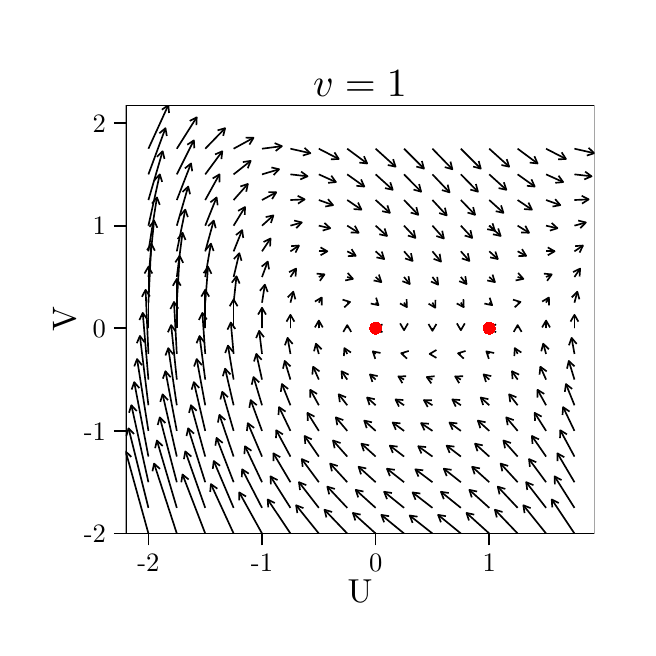
\begin{tikzpicture}[x=1pt,y=1pt]
\definecolor[named]{fillColor}{rgb}{1.00,1.00,1.00}
\path[use as bounding box,fill=fillColor,fill opacity=0.00] (0,0) rectangle (216.81,216.81);
\begin{scope}
\path[clip] (  0.00,  0.00) rectangle (216.81,216.81);
\definecolor[named]{drawColor}{rgb}{1.00,1.00,1.00}
\definecolor[named]{fillColor}{rgb}{1.00,1.00,1.00}

\path[draw=drawColor,line width= 0.6pt,line join=round,line cap=round,fill=fillColor] (  0.00,  0.00) rectangle (216.81,216.81);
\end{scope}
\begin{scope}
\path[clip] ( 35.42, 34.03) rectangle (204.76,188.82);
\definecolor[named]{fillColor}{rgb}{1.00,1.00,1.00}

\path[fill=fillColor] ( 35.42, 34.03) rectangle (204.76,188.82);
\definecolor[named]{fillColor}{rgb}{0.00,0.00,0.00}

\path[fill=fillColor,fill opacity=0.20] (166.79,145.26) circle (  0.11);

\path[fill=fillColor,fill opacity=0.20] ( 43.63, 34.03) circle (  0.11);

\path[fill=fillColor,fill opacity=0.20] ( 43.63, 43.30) circle (  0.11);

\path[fill=fillColor,fill opacity=0.20] ( 43.63, 52.57) circle (  0.11);

\path[fill=fillColor,fill opacity=0.20] ( 43.63, 61.84) circle (  0.11);

\path[fill=fillColor,fill opacity=0.20] ( 43.63, 71.11) circle (  0.11);

\path[fill=fillColor,fill opacity=0.20] ( 43.63, 80.38) circle (  0.11);

\path[fill=fillColor,fill opacity=0.20] ( 43.63, 89.65) circle (  0.11);

\path[fill=fillColor,fill opacity=0.20] ( 43.63, 98.92) circle (  0.11);

\path[fill=fillColor,fill opacity=0.20] ( 43.63,108.19) circle (  0.11);

\path[fill=fillColor,fill opacity=0.20] ( 43.63,117.45) circle (  0.11);

\path[fill=fillColor,fill opacity=0.20] ( 43.63,126.72) circle (  0.11);

\path[fill=fillColor,fill opacity=0.20] ( 43.63,135.99) circle (  0.11);

\path[fill=fillColor,fill opacity=0.20] ( 43.63,145.26) circle (  0.11);

\path[fill=fillColor,fill opacity=0.20] ( 43.63,154.53) circle (  0.11);

\path[fill=fillColor,fill opacity=0.20] ( 43.63,163.80) circle (  0.11);

\path[fill=fillColor,fill opacity=0.20] ( 43.63,173.07) circle (  0.11);

\path[fill=fillColor,fill opacity=0.20] ( 53.89, 34.03) circle (  0.11);

\path[fill=fillColor,fill opacity=0.20] ( 53.89, 43.30) circle (  0.11);

\path[fill=fillColor,fill opacity=0.20] ( 53.89, 52.57) circle (  0.11);

\path[fill=fillColor,fill opacity=0.20] ( 53.89, 61.84) circle (  0.11);

\path[fill=fillColor,fill opacity=0.20] ( 53.89, 71.11) circle (  0.11);

\path[fill=fillColor,fill opacity=0.20] ( 53.89, 80.38) circle (  0.11);

\path[fill=fillColor,fill opacity=0.20] ( 53.89, 89.65) circle (  0.11);

\path[fill=fillColor,fill opacity=0.20] ( 53.89, 98.92) circle (  0.11);

\path[fill=fillColor,fill opacity=0.20] ( 53.89,108.19) circle (  0.11);

\path[fill=fillColor,fill opacity=0.20] ( 53.89,117.45) circle (  0.11);

\path[fill=fillColor,fill opacity=0.20] ( 53.89,126.72) circle (  0.11);

\path[fill=fillColor,fill opacity=0.20] ( 53.89,135.99) circle (  0.11);

\path[fill=fillColor,fill opacity=0.20] ( 53.89,145.26) circle (  0.11);

\path[fill=fillColor,fill opacity=0.20] ( 53.89,154.53) circle (  0.11);

\path[fill=fillColor,fill opacity=0.20] ( 53.89,163.80) circle (  0.11);

\path[fill=fillColor,fill opacity=0.20] ( 53.89,173.07) circle (  0.11);

\path[fill=fillColor,fill opacity=0.20] ( 64.16, 34.03) circle (  0.11);

\path[fill=fillColor,fill opacity=0.20] ( 64.16, 43.30) circle (  0.11);

\path[fill=fillColor,fill opacity=0.20] ( 64.16, 52.57) circle (  0.11);

\path[fill=fillColor,fill opacity=0.20] ( 64.16, 61.84) circle (  0.11);

\path[fill=fillColor,fill opacity=0.20] ( 64.16, 71.11) circle (  0.11);

\path[fill=fillColor,fill opacity=0.20] ( 64.16, 80.38) circle (  0.11);

\path[fill=fillColor,fill opacity=0.20] ( 64.16, 89.65) circle (  0.11);

\path[fill=fillColor,fill opacity=0.20] ( 64.16, 98.92) circle (  0.11);

\path[fill=fillColor,fill opacity=0.20] ( 64.16,108.19) circle (  0.11);

\path[fill=fillColor,fill opacity=0.20] ( 64.16,117.45) circle (  0.11);

\path[fill=fillColor,fill opacity=0.20] ( 64.16,126.72) circle (  0.11);

\path[fill=fillColor,fill opacity=0.20] ( 64.16,135.99) circle (  0.11);

\path[fill=fillColor,fill opacity=0.20] ( 64.16,145.26) circle (  0.11);

\path[fill=fillColor,fill opacity=0.20] ( 64.16,154.53) circle (  0.11);

\path[fill=fillColor,fill opacity=0.20] ( 64.16,163.80) circle (  0.11);

\path[fill=fillColor,fill opacity=0.20] ( 64.16,173.07) circle (  0.11);

\path[fill=fillColor,fill opacity=0.20] ( 74.42, 34.03) circle (  0.11);

\path[fill=fillColor,fill opacity=0.20] ( 74.42, 43.30) circle (  0.11);

\path[fill=fillColor,fill opacity=0.20] ( 74.42, 52.57) circle (  0.11);

\path[fill=fillColor,fill opacity=0.20] ( 74.42, 61.84) circle (  0.11);

\path[fill=fillColor,fill opacity=0.20] ( 74.42, 71.11) circle (  0.11);

\path[fill=fillColor,fill opacity=0.20] ( 74.42, 80.38) circle (  0.11);

\path[fill=fillColor,fill opacity=0.20] ( 74.42, 89.65) circle (  0.11);

\path[fill=fillColor,fill opacity=0.20] ( 74.42, 98.92) circle (  0.11);

\path[fill=fillColor,fill opacity=0.20] ( 74.42,108.19) circle (  0.11);

\path[fill=fillColor,fill opacity=0.20] ( 74.42,117.45) circle (  0.11);

\path[fill=fillColor,fill opacity=0.20] ( 74.42,126.72) circle (  0.11);

\path[fill=fillColor,fill opacity=0.20] ( 74.42,135.99) circle (  0.11);

\path[fill=fillColor,fill opacity=0.20] ( 74.42,145.26) circle (  0.11);

\path[fill=fillColor,fill opacity=0.20] ( 74.42,154.53) circle (  0.11);

\path[fill=fillColor,fill opacity=0.20] ( 74.42,163.80) circle (  0.11);

\path[fill=fillColor,fill opacity=0.20] ( 74.42,173.07) circle (  0.11);

\path[fill=fillColor,fill opacity=0.20] ( 84.68, 34.03) circle (  0.11);

\path[fill=fillColor,fill opacity=0.20] ( 84.68, 43.30) circle (  0.11);

\path[fill=fillColor,fill opacity=0.20] ( 84.68, 52.57) circle (  0.11);

\path[fill=fillColor,fill opacity=0.20] ( 84.68, 61.84) circle (  0.11);

\path[fill=fillColor,fill opacity=0.20] ( 84.68, 71.11) circle (  0.11);

\path[fill=fillColor,fill opacity=0.20] ( 84.68, 80.38) circle (  0.11);

\path[fill=fillColor,fill opacity=0.20] ( 84.68, 89.65) circle (  0.11);

\path[fill=fillColor,fill opacity=0.20] ( 84.68, 98.92) circle (  0.11);

\path[fill=fillColor,fill opacity=0.20] ( 84.68,108.19) circle (  0.11);

\path[fill=fillColor,fill opacity=0.20] ( 84.68,117.45) circle (  0.11);

\path[fill=fillColor,fill opacity=0.20] ( 84.68,126.72) circle (  0.11);

\path[fill=fillColor,fill opacity=0.20] ( 84.68,135.99) circle (  0.11);

\path[fill=fillColor,fill opacity=0.20] ( 84.68,145.26) circle (  0.11);

\path[fill=fillColor,fill opacity=0.20] ( 84.68,154.53) circle (  0.11);

\path[fill=fillColor,fill opacity=0.20] ( 84.68,163.80) circle (  0.11);

\path[fill=fillColor,fill opacity=0.20] ( 84.68,173.07) circle (  0.11);

\path[fill=fillColor,fill opacity=0.20] ( 94.95, 34.03) circle (  0.11);

\path[fill=fillColor,fill opacity=0.20] ( 94.95, 43.30) circle (  0.11);

\path[fill=fillColor,fill opacity=0.20] ( 94.95, 52.57) circle (  0.11);

\path[fill=fillColor,fill opacity=0.20] ( 94.95, 61.84) circle (  0.11);

\path[fill=fillColor,fill opacity=0.20] ( 94.95, 71.11) circle (  0.11);

\path[fill=fillColor,fill opacity=0.20] ( 94.95, 80.38) circle (  0.11);

\path[fill=fillColor,fill opacity=0.20] ( 94.95, 89.65) circle (  0.11);

\path[fill=fillColor,fill opacity=0.20] ( 94.95, 98.92) circle (  0.11);

\path[fill=fillColor,fill opacity=0.20] ( 94.95,108.19) circle (  0.11);

\path[fill=fillColor,fill opacity=0.20] ( 94.95,117.45) circle (  0.11);

\path[fill=fillColor,fill opacity=0.20] ( 94.95,126.72) circle (  0.11);

\path[fill=fillColor,fill opacity=0.20] ( 94.95,135.99) circle (  0.11);

\path[fill=fillColor,fill opacity=0.20] ( 94.95,145.26) circle (  0.11);

\path[fill=fillColor,fill opacity=0.20] ( 94.95,154.53) circle (  0.11);

\path[fill=fillColor,fill opacity=0.20] ( 94.95,163.80) circle (  0.11);

\path[fill=fillColor,fill opacity=0.20] ( 94.95,173.07) circle (  0.11);

\path[fill=fillColor,fill opacity=0.20] (105.21, 34.03) circle (  0.11);

\path[fill=fillColor,fill opacity=0.20] (105.21, 43.30) circle (  0.11);

\path[fill=fillColor,fill opacity=0.20] (105.21, 52.57) circle (  0.11);

\path[fill=fillColor,fill opacity=0.20] (105.21, 61.84) circle (  0.11);

\path[fill=fillColor,fill opacity=0.20] (105.21, 71.11) circle (  0.11);

\path[fill=fillColor,fill opacity=0.20] (105.21, 80.38) circle (  0.11);

\path[fill=fillColor,fill opacity=0.20] (105.21, 89.65) circle (  0.11);

\path[fill=fillColor,fill opacity=0.20] (105.21, 98.92) circle (  0.11);

\path[fill=fillColor,fill opacity=0.20] (105.21,108.19) circle (  0.11);

\path[fill=fillColor,fill opacity=0.20] (105.21,117.45) circle (  0.11);

\path[fill=fillColor,fill opacity=0.20] (105.21,126.72) circle (  0.11);

\path[fill=fillColor,fill opacity=0.20] (105.21,135.99) circle (  0.11);

\path[fill=fillColor,fill opacity=0.20] (105.21,145.26) circle (  0.11);

\path[fill=fillColor,fill opacity=0.20] (105.21,154.53) circle (  0.11);

\path[fill=fillColor,fill opacity=0.20] (105.21,163.80) circle (  0.11);

\path[fill=fillColor,fill opacity=0.20] (105.21,173.07) circle (  0.11);

\path[fill=fillColor,fill opacity=0.20] (115.47, 34.03) circle (  0.11);

\path[fill=fillColor,fill opacity=0.20] (115.47, 43.30) circle (  0.11);

\path[fill=fillColor,fill opacity=0.20] (115.47, 52.57) circle (  0.11);

\path[fill=fillColor,fill opacity=0.20] (115.47, 61.84) circle (  0.11);

\path[fill=fillColor,fill opacity=0.20] (115.47, 71.11) circle (  0.11);

\path[fill=fillColor,fill opacity=0.20] (115.47, 80.38) circle (  0.11);

\path[fill=fillColor,fill opacity=0.20] (115.47, 89.65) circle (  0.11);

\path[fill=fillColor,fill opacity=0.20] (115.47, 98.92) circle (  0.11);

\path[fill=fillColor,fill opacity=0.20] (115.47,108.19) circle (  0.11);

\path[fill=fillColor,fill opacity=0.20] (115.47,117.45) circle (  0.11);

\path[fill=fillColor,fill opacity=0.20] (115.47,126.72) circle (  0.11);

\path[fill=fillColor,fill opacity=0.20] (115.47,135.99) circle (  0.11);

\path[fill=fillColor,fill opacity=0.20] (115.47,145.26) circle (  0.11);

\path[fill=fillColor,fill opacity=0.20] (115.47,154.53) circle (  0.11);

\path[fill=fillColor,fill opacity=0.20] (115.47,163.80) circle (  0.11);

\path[fill=fillColor,fill opacity=0.20] (115.47,173.07) circle (  0.11);

\path[fill=fillColor,fill opacity=0.20] (125.74, 34.03) circle (  0.11);

\path[fill=fillColor,fill opacity=0.20] (125.74, 43.30) circle (  0.11);

\path[fill=fillColor,fill opacity=0.20] (125.74, 52.57) circle (  0.11);

\path[fill=fillColor,fill opacity=0.20] (125.74, 61.84) circle (  0.11);

\path[fill=fillColor,fill opacity=0.20] (125.74, 71.11) circle (  0.11);

\path[fill=fillColor,fill opacity=0.20] (125.74, 80.38) circle (  0.11);

\path[fill=fillColor,fill opacity=0.20] (125.74, 89.65) circle (  0.11);

\path[fill=fillColor,fill opacity=0.20] (125.74, 98.92) circle (  0.11);

\path[fill=fillColor,fill opacity=0.20] (125.74,108.19) circle (  0.11);

\path[fill=fillColor,fill opacity=0.20] (125.74,117.45) circle (  0.11);

\path[fill=fillColor,fill opacity=0.20] (125.74,126.72) circle (  0.11);

\path[fill=fillColor,fill opacity=0.20] (125.74,135.99) circle (  0.11);

\path[fill=fillColor,fill opacity=0.20] (125.74,145.26) circle (  0.11);

\path[fill=fillColor,fill opacity=0.20] (125.74,154.53) circle (  0.11);

\path[fill=fillColor,fill opacity=0.20] (125.74,163.80) circle (  0.11);

\path[fill=fillColor,fill opacity=0.20] (125.74,173.07) circle (  0.11);

\path[fill=fillColor,fill opacity=0.20] (136.00, 34.03) circle (  0.11);

\path[fill=fillColor,fill opacity=0.20] (136.00, 43.30) circle (  0.11);

\path[fill=fillColor,fill opacity=0.20] (136.00, 52.57) circle (  0.11);

\path[fill=fillColor,fill opacity=0.20] (136.00, 61.84) circle (  0.11);

\path[fill=fillColor,fill opacity=0.20] (136.00, 71.11) circle (  0.11);

\path[fill=fillColor,fill opacity=0.20] (136.00, 80.38) circle (  0.11);

\path[fill=fillColor,fill opacity=0.20] (136.00, 89.65) circle (  0.11);

\path[fill=fillColor,fill opacity=0.20] (136.00, 98.92) circle (  0.11);

\path[fill=fillColor,fill opacity=0.20] (136.00,108.19) circle (  0.11);

\path[fill=fillColor,fill opacity=0.20] (136.00,117.45) circle (  0.11);

\path[fill=fillColor,fill opacity=0.20] (136.00,126.72) circle (  0.11);

\path[fill=fillColor,fill opacity=0.20] (136.00,135.99) circle (  0.11);

\path[fill=fillColor,fill opacity=0.20] (136.00,145.26) circle (  0.11);

\path[fill=fillColor,fill opacity=0.20] (136.00,154.53) circle (  0.11);

\path[fill=fillColor,fill opacity=0.20] (136.00,163.80) circle (  0.11);

\path[fill=fillColor,fill opacity=0.20] (136.00,173.07) circle (  0.11);

\path[fill=fillColor,fill opacity=0.20] (146.26, 34.03) circle (  0.11);

\path[fill=fillColor,fill opacity=0.20] (146.26, 43.30) circle (  0.11);

\path[fill=fillColor,fill opacity=0.20] (146.26, 52.57) circle (  0.11);

\path[fill=fillColor,fill opacity=0.20] (146.26, 61.84) circle (  0.11);

\path[fill=fillColor,fill opacity=0.20] (146.26, 71.11) circle (  0.11);

\path[fill=fillColor,fill opacity=0.20] (146.26, 80.38) circle (  0.11);

\path[fill=fillColor,fill opacity=0.20] (146.26, 89.65) circle (  0.11);

\path[fill=fillColor,fill opacity=0.20] (146.26, 98.92) circle (  0.11);

\path[fill=fillColor,fill opacity=0.20] (146.26,108.19) circle (  0.11);

\path[fill=fillColor,fill opacity=0.20] (146.26,117.45) circle (  0.11);

\path[fill=fillColor,fill opacity=0.20] (146.26,126.72) circle (  0.11);

\path[fill=fillColor,fill opacity=0.20] (146.26,135.99) circle (  0.11);

\path[fill=fillColor,fill opacity=0.20] (146.26,145.26) circle (  0.11);

\path[fill=fillColor,fill opacity=0.20] (146.26,154.53) circle (  0.11);

\path[fill=fillColor,fill opacity=0.20] (146.26,163.80) circle (  0.11);

\path[fill=fillColor,fill opacity=0.20] (146.26,173.07) circle (  0.11);

\path[fill=fillColor,fill opacity=0.20] (156.53, 34.03) circle (  0.11);

\path[fill=fillColor,fill opacity=0.20] (156.53, 43.30) circle (  0.11);

\path[fill=fillColor,fill opacity=0.20] (156.53, 52.57) circle (  0.11);

\path[fill=fillColor,fill opacity=0.20] (156.53, 61.84) circle (  0.11);

\path[fill=fillColor,fill opacity=0.20] (156.53, 71.11) circle (  0.11);

\path[fill=fillColor,fill opacity=0.20] (156.53, 80.38) circle (  0.11);

\path[fill=fillColor,fill opacity=0.20] (156.53, 89.65) circle (  0.11);

\path[fill=fillColor,fill opacity=0.20] (156.53, 98.92) circle (  0.11);

\path[fill=fillColor,fill opacity=0.20] (156.53,108.19) circle (  0.11);

\path[fill=fillColor,fill opacity=0.20] (156.53,117.45) circle (  0.11);

\path[fill=fillColor,fill opacity=0.20] (156.53,126.72) circle (  0.11);

\path[fill=fillColor,fill opacity=0.20] (156.53,135.99) circle (  0.11);

\path[fill=fillColor,fill opacity=0.20] (156.53,145.26) circle (  0.11);

\path[fill=fillColor,fill opacity=0.20] (156.53,154.53) circle (  0.11);

\path[fill=fillColor,fill opacity=0.20] (156.53,163.80) circle (  0.11);

\path[fill=fillColor,fill opacity=0.20] (156.53,173.07) circle (  0.11);

\path[fill=fillColor,fill opacity=0.20] (166.79, 34.03) circle (  0.11);

\path[fill=fillColor,fill opacity=0.20] (166.79, 43.30) circle (  0.11);

\path[fill=fillColor,fill opacity=0.20] (166.79, 52.57) circle (  0.11);

\path[fill=fillColor,fill opacity=0.20] (166.79, 61.84) circle (  0.11);

\path[fill=fillColor,fill opacity=0.20] (166.79, 71.11) circle (  0.11);

\path[fill=fillColor,fill opacity=0.20] (166.79, 80.38) circle (  0.11);

\path[fill=fillColor,fill opacity=0.20] (166.79, 89.65) circle (  0.11);

\path[fill=fillColor,fill opacity=0.20] (166.79, 98.92) circle (  0.11);

\path[fill=fillColor,fill opacity=0.20] (166.79,108.19) circle (  0.11);

\path[fill=fillColor,fill opacity=0.20] (166.79,117.45) circle (  0.11);

\path[fill=fillColor,fill opacity=0.20] (166.79,126.72) circle (  0.11);

\path[fill=fillColor,fill opacity=0.20] (166.79,135.99) circle (  0.11);

\path[fill=fillColor,fill opacity=0.20] (166.79,145.26) circle (  0.11);

\path[fill=fillColor,fill opacity=0.20] (166.79,154.53) circle (  0.11);

\path[fill=fillColor,fill opacity=0.20] (166.79,163.80) circle (  0.11);

\path[fill=fillColor,fill opacity=0.20] (166.79,173.07) circle (  0.11);

\path[fill=fillColor,fill opacity=0.20] (177.05, 34.03) circle (  0.11);

\path[fill=fillColor,fill opacity=0.20] (177.05, 43.30) circle (  0.11);

\path[fill=fillColor,fill opacity=0.20] (177.05, 52.57) circle (  0.11);

\path[fill=fillColor,fill opacity=0.20] (177.05, 61.84) circle (  0.11);

\path[fill=fillColor,fill opacity=0.20] (177.05, 71.11) circle (  0.11);

\path[fill=fillColor,fill opacity=0.20] (177.05, 80.38) circle (  0.11);

\path[fill=fillColor,fill opacity=0.20] (177.05, 89.65) circle (  0.11);

\path[fill=fillColor,fill opacity=0.20] (177.05, 98.92) circle (  0.11);

\path[fill=fillColor,fill opacity=0.20] (177.05,108.19) circle (  0.11);

\path[fill=fillColor,fill opacity=0.20] (177.05,117.45) circle (  0.11);

\path[fill=fillColor,fill opacity=0.20] (177.05,126.72) circle (  0.11);

\path[fill=fillColor,fill opacity=0.20] (177.05,135.99) circle (  0.11);

\path[fill=fillColor,fill opacity=0.20] (177.05,145.26) circle (  0.11);

\path[fill=fillColor,fill opacity=0.20] (177.05,154.53) circle (  0.11);

\path[fill=fillColor,fill opacity=0.20] (177.05,163.80) circle (  0.11);

\path[fill=fillColor,fill opacity=0.20] (177.05,173.07) circle (  0.11);

\path[fill=fillColor,fill opacity=0.20] (187.32, 34.03) circle (  0.11);

\path[fill=fillColor,fill opacity=0.20] (187.32, 43.30) circle (  0.11);

\path[fill=fillColor,fill opacity=0.20] (187.32, 52.57) circle (  0.11);

\path[fill=fillColor,fill opacity=0.20] (187.32, 61.84) circle (  0.11);

\path[fill=fillColor,fill opacity=0.20] (187.32, 71.11) circle (  0.11);

\path[fill=fillColor,fill opacity=0.20] (187.32, 80.38) circle (  0.11);

\path[fill=fillColor,fill opacity=0.20] (187.32, 89.65) circle (  0.11);

\path[fill=fillColor,fill opacity=0.20] (187.32, 98.92) circle (  0.11);

\path[fill=fillColor,fill opacity=0.20] (187.32,108.19) circle (  0.11);

\path[fill=fillColor,fill opacity=0.20] (187.32,117.45) circle (  0.11);

\path[fill=fillColor,fill opacity=0.20] (187.32,126.72) circle (  0.11);

\path[fill=fillColor,fill opacity=0.20] (187.32,135.99) circle (  0.11);

\path[fill=fillColor,fill opacity=0.20] (187.32,145.26) circle (  0.11);

\path[fill=fillColor,fill opacity=0.20] (187.32,154.53) circle (  0.11);

\path[fill=fillColor,fill opacity=0.20] (187.32,163.80) circle (  0.11);

\path[fill=fillColor,fill opacity=0.20] (187.32,173.07) circle (  0.11);

\path[fill=fillColor,fill opacity=0.20] (197.58, 34.03) circle (  0.11);

\path[fill=fillColor,fill opacity=0.20] (197.58, 43.30) circle (  0.11);

\path[fill=fillColor,fill opacity=0.20] (197.58, 52.57) circle (  0.11);

\path[fill=fillColor,fill opacity=0.20] (197.58, 61.84) circle (  0.11);

\path[fill=fillColor,fill opacity=0.20] (197.58, 71.11) circle (  0.11);

\path[fill=fillColor,fill opacity=0.20] (197.58, 80.38) circle (  0.11);

\path[fill=fillColor,fill opacity=0.20] (197.58, 89.65) circle (  0.11);

\path[fill=fillColor,fill opacity=0.20] (197.58, 98.92) circle (  0.11);

\path[fill=fillColor,fill opacity=0.20] (197.58,108.19) circle (  0.11);

\path[fill=fillColor,fill opacity=0.20] (197.58,117.45) circle (  0.11);

\path[fill=fillColor,fill opacity=0.20] (197.58,126.72) circle (  0.11);

\path[fill=fillColor,fill opacity=0.20] (197.58,135.99) circle (  0.11);

\path[fill=fillColor,fill opacity=0.20] (197.58,145.26) circle (  0.11);

\path[fill=fillColor,fill opacity=0.20] (197.58,154.53) circle (  0.11);

\path[fill=fillColor,fill opacity=0.20] (197.58,163.80) circle (  0.11);

\path[fill=fillColor,fill opacity=0.20] (197.58,173.07) circle (  0.11);
\definecolor[named]{drawColor}{rgb}{0.00,0.00,0.00}
\definecolor[named]{fillColor}{rgb}{0.00,0.00,0.00}

\path[draw=drawColor,line width= 0.6pt,line join=round,fill=fillColor] (166.79,145.26) -- (168.84,143.41);

\path[draw=drawColor,line width= 0.6pt,line join=round] (166.06,144.00) --
	(168.84,143.41) --
	(167.97,146.11);

\path[draw=drawColor,line width= 0.6pt,line join=round,fill=fillColor] ( 43.63, 34.03) -- ( 35.42, 63.69);

\path[draw=drawColor,line width= 0.6pt,line join=round] ( 37.45, 61.70) --
	( 35.42, 63.69) --
	( 34.71, 60.94);

\path[draw=drawColor,line width= 0.6pt,line join=round,fill=fillColor] ( 43.63, 43.30) -- ( 36.45, 72.04);

\path[draw=drawColor,line width= 0.6pt,line join=round] ( 38.43, 69.99) --
	( 36.45, 72.04) --
	( 35.66, 69.30);

\path[draw=drawColor,line width= 0.6pt,line join=round,fill=fillColor] ( 43.63, 52.57) -- ( 37.47, 80.38);

\path[draw=drawColor,line width= 0.6pt,line join=round] ( 39.40, 78.28) --
	( 37.47, 80.38) --
	( 36.62, 77.67);

\path[draw=drawColor,line width= 0.6pt,line join=round,fill=fillColor] ( 43.63, 61.84) -- ( 38.50, 88.72);

\path[draw=drawColor,line width= 0.6pt,line join=round] ( 40.36, 86.57) --
	( 38.50, 88.72) --
	( 37.56, 86.03);

\path[draw=drawColor,line width= 0.6pt,line join=round,fill=fillColor] ( 43.63, 71.11) -- ( 39.53, 97.06);

\path[draw=drawColor,line width= 0.6pt,line join=round] ( 41.32, 94.85) --
	( 39.53, 97.06) --
	( 38.51, 94.41);

\path[draw=drawColor,line width= 0.6pt,line join=round,fill=fillColor] ( 43.63, 80.38) -- ( 40.55,105.40);

\path[draw=drawColor,line width= 0.6pt,line join=round] ( 42.27,103.13) --
	( 40.55,105.40) --
	( 39.44,102.79);

\path[draw=drawColor,line width= 0.6pt,line join=round,fill=fillColor] ( 43.63, 89.65) -- ( 41.58,113.75);

\path[draw=drawColor,line width= 0.6pt,line join=round] ( 43.21,111.41) --
	( 41.58,113.75) --
	( 40.37,111.17);

\path[draw=drawColor,line width= 0.6pt,line join=round,fill=fillColor] ( 43.63, 98.92) -- ( 42.61,122.09);

\path[draw=drawColor,line width= 0.6pt,line join=round] ( 44.14,119.69) --
	( 42.61,122.09) --
	( 41.29,119.56);

\path[draw=drawColor,line width= 0.6pt,line join=round,fill=fillColor] ( 43.63,108.19) -- ( 43.63,130.43);

\path[draw=drawColor,line width= 0.6pt,line join=round] ( 45.05,127.97) --
	( 43.63,130.43) --
	( 42.21,127.97);

\path[draw=drawColor,line width= 0.6pt,line join=round,fill=fillColor] ( 43.63,117.45) -- ( 44.66,138.77);

\path[draw=drawColor,line width= 0.6pt,line join=round] ( 45.96,136.24) --
	( 44.66,138.77) --
	( 43.12,136.38);

\path[draw=drawColor,line width= 0.6pt,line join=round,fill=fillColor] ( 43.63,126.72) -- ( 45.68,147.11);

\path[draw=drawColor,line width= 0.6pt,line join=round] ( 46.85,144.52) --
	( 45.68,147.11) --
	( 44.02,144.81);

\path[draw=drawColor,line width= 0.6pt,line join=round,fill=fillColor] ( 43.63,135.99) -- ( 46.71,155.46);

\path[draw=drawColor,line width= 0.6pt,line join=round] ( 47.73,152.80) --
	( 46.71,155.46) --
	( 44.92,153.25);

\path[draw=drawColor,line width= 0.6pt,line join=round,fill=fillColor] ( 43.63,145.26) -- ( 47.74,163.80);

\path[draw=drawColor,line width= 0.6pt,line join=round] ( 48.59,161.09) --
	( 47.74,163.80) --
	( 45.82,161.70);

\path[draw=drawColor,line width= 0.6pt,line join=round,fill=fillColor] ( 43.63,154.53) -- ( 48.76,172.14);

\path[draw=drawColor,line width= 0.6pt,line join=round] ( 49.44,169.38) --
	( 48.76,172.14) --
	( 46.71,170.17);

\path[draw=drawColor,line width= 0.6pt,line join=round,fill=fillColor] ( 43.63,163.80) -- ( 49.79,180.48);

\path[draw=drawColor,line width= 0.6pt,line join=round] ( 50.27,177.68) --
	( 49.79,180.48) --
	( 47.60,178.66);

\path[draw=drawColor,line width= 0.6pt,line join=round,fill=fillColor] ( 43.63,173.07) -- ( 50.82,188.82);

\path[draw=drawColor,line width= 0.6pt,line join=round] ( 51.09,185.99) --
	( 50.82,188.82) --
	( 48.50,187.17);

\path[draw=drawColor,line width= 0.6pt,line join=round,fill=fillColor] ( 53.89, 34.03) -- ( 45.68, 59.29);

\path[draw=drawColor,line width= 0.6pt,line join=round] ( 47.80, 57.39) --
	( 45.68, 59.29) --
	( 45.09, 56.51);

\path[draw=drawColor,line width= 0.6pt,line join=round,fill=fillColor] ( 53.89, 43.30) -- ( 46.71, 67.63);

\path[draw=drawColor,line width= 0.6pt,line join=round] ( 48.77, 65.67) --
	( 46.71, 67.63) --
	( 46.04, 64.87);

\path[draw=drawColor,line width= 0.6pt,line join=round,fill=fillColor] ( 53.89, 52.57) -- ( 47.74, 75.98);

\path[draw=drawColor,line width= 0.6pt,line join=round] ( 49.74, 73.96) --
	( 47.74, 75.98) --
	( 46.99, 73.23);

\path[draw=drawColor,line width= 0.6pt,line join=round,fill=fillColor] ( 53.89, 61.84) -- ( 48.76, 84.32);

\path[draw=drawColor,line width= 0.6pt,line join=round] ( 50.70, 82.23) --
	( 48.76, 84.32) --
	( 47.92, 81.60);

\path[draw=drawColor,line width= 0.6pt,line join=round,fill=fillColor] ( 53.89, 71.11) -- ( 49.79, 92.66);

\path[draw=drawColor,line width= 0.6pt,line join=round] ( 51.65, 90.51) --
	( 49.79, 92.66) --
	( 48.85, 89.97);

\path[draw=drawColor,line width= 0.6pt,line join=round,fill=fillColor] ( 53.89, 80.38) -- ( 50.82,101.00);

\path[draw=drawColor,line width= 0.6pt,line join=round] ( 52.59, 98.78) --
	( 50.82,101.00) --
	( 49.77, 98.36);

\path[draw=drawColor,line width= 0.6pt,line join=round,fill=fillColor] ( 53.89, 89.65) -- ( 51.84,109.34);

\path[draw=drawColor,line width= 0.6pt,line join=round] ( 53.51,107.04) --
	( 51.84,109.34) --
	( 50.68,106.75);

\path[draw=drawColor,line width= 0.6pt,line join=round,fill=fillColor] ( 53.89, 98.92) -- ( 52.87,117.69);

\path[draw=drawColor,line width= 0.6pt,line join=round] ( 54.42,115.30) --
	( 52.87,117.69) --
	( 51.58,115.15);

\path[draw=drawColor,line width= 0.6pt,line join=round,fill=fillColor] ( 53.89,108.19) -- ( 53.89,126.03);

\path[draw=drawColor,line width= 0.6pt,line join=round] ( 55.32,123.56) --
	( 53.89,126.03) --
	( 52.47,123.56);

\path[draw=drawColor,line width= 0.6pt,line join=round,fill=fillColor] ( 53.89,117.45) -- ( 54.92,134.37);

\path[draw=drawColor,line width= 0.6pt,line join=round] ( 56.19,131.82) --
	( 54.92,134.37) --
	( 53.35,132.00);

\path[draw=drawColor,line width= 0.6pt,line join=round,fill=fillColor] ( 53.89,126.72) -- ( 55.95,142.71);

\path[draw=drawColor,line width= 0.6pt,line join=round] ( 57.04,140.09) --
	( 55.95,142.71) --
	( 54.22,140.45);

\path[draw=drawColor,line width= 0.6pt,line join=round,fill=fillColor] ( 53.89,135.99) -- ( 56.97,151.05);

\path[draw=drawColor,line width= 0.6pt,line join=round] ( 57.87,148.36) --
	( 56.97,151.05) --
	( 55.09,148.92);

\path[draw=drawColor,line width= 0.6pt,line join=round,fill=fillColor] ( 53.89,145.26) -- ( 58.00,159.40);

\path[draw=drawColor,line width= 0.6pt,line join=round] ( 58.68,156.63) --
	( 58.00,159.40) --
	( 55.95,157.43);

\path[draw=drawColor,line width= 0.6pt,line join=round,fill=fillColor] ( 53.89,154.53) -- ( 59.03,167.74);

\path[draw=drawColor,line width= 0.6pt,line join=round] ( 59.46,164.93) --
	( 59.03,167.74) --
	( 56.81,165.96);

\path[draw=drawColor,line width= 0.6pt,line join=round,fill=fillColor] ( 53.89,163.80) -- ( 60.05,176.08);

\path[draw=drawColor,line width= 0.6pt,line join=round] ( 60.22,173.24) --
	( 60.05,176.08) --
	( 57.68,174.52);

\path[draw=drawColor,line width= 0.6pt,line join=round,fill=fillColor] ( 53.89,173.07) -- ( 61.08,184.42);

\path[draw=drawColor,line width= 0.6pt,line join=round] ( 60.96,181.58) --
	( 61.08,184.42) --
	( 58.56,183.10);

\path[draw=drawColor,line width= 0.6pt,line join=round,fill=fillColor] ( 64.16, 34.03) -- ( 55.95, 55.35);

\path[draw=drawColor,line width= 0.6pt,line join=round] ( 58.16, 53.56) --
	( 55.95, 55.35) --
	( 55.51, 52.54);

\path[draw=drawColor,line width= 0.6pt,line join=round,fill=fillColor] ( 64.16, 43.30) -- ( 56.97, 63.69);

\path[draw=drawColor,line width= 0.6pt,line join=round] ( 59.13, 61.84) --
	( 56.97, 63.69) --
	( 56.45, 60.90);

\path[draw=drawColor,line width= 0.6pt,line join=round,fill=fillColor] ( 64.16, 52.57) -- ( 58.00, 72.04);

\path[draw=drawColor,line width= 0.6pt,line join=round] ( 60.10, 70.12) --
	( 58.00, 72.04) --
	( 57.39, 69.26);

\path[draw=drawColor,line width= 0.6pt,line join=round,fill=fillColor] ( 64.16, 61.84) -- ( 59.03, 80.38);

\path[draw=drawColor,line width= 0.6pt,line join=round] ( 61.05, 78.38) --
	( 59.03, 80.38) --
	( 58.31, 77.62);

\path[draw=drawColor,line width= 0.6pt,line join=round,fill=fillColor] ( 64.16, 71.11) -- ( 60.05, 88.72);

\path[draw=drawColor,line width= 0.6pt,line join=round] ( 62.00, 86.64) --
	( 60.05, 88.72) --
	( 59.23, 86.00);

\path[draw=drawColor,line width= 0.6pt,line join=round,fill=fillColor] ( 64.16, 80.38) -- ( 61.08, 97.06);

\path[draw=drawColor,line width= 0.6pt,line join=round] ( 62.93, 94.90) --
	( 61.08, 97.06) --
	( 60.13, 94.38);

\path[draw=drawColor,line width= 0.6pt,line join=round,fill=fillColor] ( 64.16, 89.65) -- ( 62.11,105.40);

\path[draw=drawColor,line width= 0.6pt,line join=round] ( 63.83,103.15) --
	( 62.11,105.40) --
	( 61.01,102.78);

\path[draw=drawColor,line width= 0.6pt,line join=round,fill=fillColor] ( 64.16, 98.92) -- ( 63.13,113.75);

\path[draw=drawColor,line width= 0.6pt,line join=round] ( 64.72,111.39) --
	( 63.13,113.75) --
	( 61.88,111.19);

\path[draw=drawColor,line width= 0.6pt,line join=round,fill=fillColor] ( 64.16,108.19) -- ( 64.16,122.09);

\path[draw=drawColor,line width= 0.6pt,line join=round] ( 65.58,119.62) --
	( 64.16,122.09) --
	( 62.74,119.62);

\path[draw=drawColor,line width= 0.6pt,line join=round,fill=fillColor] ( 64.16,117.45) -- ( 65.18,130.43);

\path[draw=drawColor,line width= 0.6pt,line join=round] ( 66.41,127.86) --
	( 65.18,130.43) --
	( 63.57,128.09);

\path[draw=drawColor,line width= 0.6pt,line join=round,fill=fillColor] ( 64.16,126.72) -- ( 66.21,138.77);

\path[draw=drawColor,line width= 0.6pt,line join=round] ( 67.20,136.10) --
	( 66.21,138.77) --
	( 64.39,136.58);

\path[draw=drawColor,line width= 0.6pt,line join=round,fill=fillColor] ( 64.16,135.99) -- ( 67.24,147.11);

\path[draw=drawColor,line width= 0.6pt,line join=round] ( 67.95,144.36) --
	( 67.24,147.11) --
	( 65.21,145.12);

\path[draw=drawColor,line width= 0.6pt,line join=round,fill=fillColor] ( 64.16,145.26) -- ( 68.26,155.46);

\path[draw=drawColor,line width= 0.6pt,line join=round] ( 68.66,152.64) --
	( 68.26,155.46) --
	( 66.02,153.70);

\path[draw=drawColor,line width= 0.6pt,line join=round,fill=fillColor] ( 64.16,154.53) -- ( 69.29,163.80);

\path[draw=drawColor,line width= 0.6pt,line join=round] ( 69.34,160.95) --
	( 69.29,163.80) --
	( 66.85,162.33);

\path[draw=drawColor,line width= 0.6pt,line join=round,fill=fillColor] ( 64.16,163.80) -- ( 70.32,172.14);

\path[draw=drawColor,line width= 0.6pt,line join=round] ( 70.00,169.31) --
	( 70.32,172.14) --
	( 67.71,171.00);

\path[draw=drawColor,line width= 0.6pt,line join=round,fill=fillColor] ( 64.16,173.07) -- ( 71.34,180.48);

\path[draw=drawColor,line width= 0.6pt,line join=round] ( 70.65,177.72) --
	( 71.34,180.48) --
	( 68.61,179.70);

\path[draw=drawColor,line width= 0.6pt,line join=round,fill=fillColor] ( 74.42, 34.03) -- ( 66.21, 51.88);

\path[draw=drawColor,line width= 0.6pt,line join=round] ( 68.53, 50.23) --
	( 66.21, 51.88) --
	( 65.95, 49.04);

\path[draw=drawColor,line width= 0.6pt,line join=round,fill=fillColor] ( 74.42, 43.30) -- ( 67.24, 60.22);

\path[draw=drawColor,line width= 0.6pt,line join=round] ( 69.51, 58.51) --
	( 67.24, 60.22) --
	( 66.89, 57.40);

\path[draw=drawColor,line width= 0.6pt,line join=round,fill=fillColor] ( 74.42, 52.57) -- ( 68.26, 68.56);

\path[draw=drawColor,line width= 0.6pt,line join=round] ( 70.48, 66.77) --
	( 68.26, 68.56) --
	( 67.82, 65.75);

\path[draw=drawColor,line width= 0.6pt,line join=round,fill=fillColor] ( 74.42, 61.84) -- ( 69.29, 76.90);

\path[draw=drawColor,line width= 0.6pt,line join=round] ( 71.43, 75.03) --
	( 69.29, 76.90) --
	( 68.74, 74.11);

\path[draw=drawColor,line width= 0.6pt,line join=round,fill=fillColor] ( 74.42, 71.11) -- ( 70.32, 85.25);

\path[draw=drawColor,line width= 0.6pt,line join=round] ( 72.37, 83.28) --
	( 70.32, 85.25) --
	( 69.64, 82.48);

\path[draw=drawColor,line width= 0.6pt,line join=round,fill=fillColor] ( 74.42, 80.38) -- ( 71.34, 93.59);

\path[draw=drawColor,line width= 0.6pt,line join=round] ( 73.29, 91.51) --
	( 71.34, 93.59) --
	( 70.52, 90.86);

\path[draw=drawColor,line width= 0.6pt,line join=round,fill=fillColor] ( 74.42, 89.65) -- ( 72.37,101.93);

\path[draw=drawColor,line width= 0.6pt,line join=round] ( 74.18, 99.73) --
	( 72.37,101.93) --
	( 71.37, 99.26);

\path[draw=drawColor,line width= 0.6pt,line join=round,fill=fillColor] ( 74.42, 98.92) -- ( 73.40,110.27);

\path[draw=drawColor,line width= 0.6pt,line join=round] ( 75.03,107.95) --
	( 73.40,110.27) --
	( 72.20,107.69);

\path[draw=drawColor,line width= 0.6pt,line join=round,fill=fillColor] ( 74.42,108.19) -- ( 74.42,118.61);

\path[draw=drawColor,line width= 0.6pt,line join=round] ( 75.84,116.15) --
	( 74.42,118.61) --
	( 73.00,116.15);

\path[draw=drawColor,line width= 0.6pt,line join=round,fill=fillColor] ( 74.42,117.45) -- ( 75.45,126.96);

\path[draw=drawColor,line width= 0.6pt,line join=round] ( 76.60,124.35) --
	( 75.45,126.96) --
	( 73.77,124.66);

\path[draw=drawColor,line width= 0.6pt,line join=round,fill=fillColor] ( 74.42,126.72) -- ( 76.47,135.30);

\path[draw=drawColor,line width= 0.6pt,line join=round] ( 77.28,132.57) --
	( 76.47,135.30) --
	( 74.52,133.23);

\path[draw=drawColor,line width= 0.6pt,line join=round,fill=fillColor] ( 74.42,135.99) -- ( 77.50,143.64);

\path[draw=drawColor,line width= 0.6pt,line join=round] ( 77.90,140.82) --
	( 77.50,143.64) --
	( 75.26,141.88);

\path[draw=drawColor,line width= 0.6pt,line join=round,fill=fillColor] ( 74.42,145.26) -- ( 78.53,151.98);

\path[draw=drawColor,line width= 0.6pt,line join=round] ( 78.46,149.14) --
	( 78.53,151.98) --
	( 76.03,150.62);

\path[draw=drawColor,line width= 0.6pt,line join=round,fill=fillColor] ( 74.42,154.53) -- ( 79.55,160.32);

\path[draw=drawColor,line width= 0.6pt,line join=round] ( 78.98,157.54) --
	( 79.55,160.32) --
	( 76.85,159.42);

\path[draw=drawColor,line width= 0.6pt,line join=round,fill=fillColor] ( 74.42,163.80) -- ( 80.58,168.67);

\path[draw=drawColor,line width= 0.6pt,line join=round] ( 79.53,166.02) --
	( 80.58,168.67) --
	( 77.76,168.25);

\path[draw=drawColor,line width= 0.6pt,line join=round,fill=fillColor] ( 74.42,173.07) -- ( 81.61,177.01);

\path[draw=drawColor,line width= 0.6pt,line join=round] ( 80.13,174.57) --
	( 81.61,177.01) --
	( 78.76,177.07);

\path[draw=drawColor,line width= 0.6pt,line join=round,fill=fillColor] ( 84.68, 34.03) -- ( 76.47, 48.86);

\path[draw=drawColor,line width= 0.6pt,line join=round] ( 78.91, 47.40) --
	( 76.47, 48.86) --
	( 76.42, 46.02);

\path[draw=drawColor,line width= 0.6pt,line join=round,fill=fillColor] ( 84.68, 43.30) -- ( 77.50, 57.21);

\path[draw=drawColor,line width= 0.6pt,line join=round] ( 79.90, 55.67) --
	( 77.50, 57.21) --
	( 77.37, 54.36);

\path[draw=drawColor,line width= 0.6pt,line join=round,fill=fillColor] ( 84.68, 52.57) -- ( 78.53, 65.55);

\path[draw=drawColor,line width= 0.6pt,line join=round] ( 80.87, 63.93) --
	( 78.53, 65.55) --
	( 78.30, 62.71);

\path[draw=drawColor,line width= 0.6pt,line join=round,fill=fillColor] ( 84.68, 61.84) -- ( 79.55, 73.89);

\path[draw=drawColor,line width= 0.6pt,line join=round] ( 81.83, 72.18) --
	( 79.55, 73.89) --
	( 79.21, 71.07);

\path[draw=drawColor,line width= 0.6pt,line join=round,fill=fillColor] ( 84.68, 71.11) -- ( 80.58, 82.23);

\path[draw=drawColor,line width= 0.6pt,line join=round] ( 82.77, 80.41) --
	( 80.58, 82.23) --
	( 80.10, 79.43);

\path[draw=drawColor,line width= 0.6pt,line join=round,fill=fillColor] ( 84.68, 80.38) -- ( 81.61, 90.57);

\path[draw=drawColor,line width= 0.6pt,line join=round] ( 83.68, 88.63) --
	( 81.61, 90.57) --
	( 80.96, 87.80);

\path[draw=drawColor,line width= 0.6pt,line join=round,fill=fillColor] ( 84.68, 89.65) -- ( 82.63, 98.92);

\path[draw=drawColor,line width= 0.6pt,line join=round] ( 84.55, 96.82) --
	( 82.63, 98.92) --
	( 81.78, 96.20);

\path[draw=drawColor,line width= 0.6pt,line join=round,fill=fillColor] ( 84.68, 98.92) -- ( 83.66,107.26);

\path[draw=drawColor,line width= 0.6pt,line join=round] ( 85.37,104.99) --
	( 83.66,107.26) --
	( 82.55,104.64);

\path[draw=drawColor,line width= 0.6pt,line join=round,fill=fillColor] ( 84.68,108.19) -- ( 84.68,115.60);

\path[draw=drawColor,line width= 0.6pt,line join=round] ( 86.11,113.14) --
	( 84.68,115.60) --
	( 83.26,113.14);

\path[draw=drawColor,line width= 0.6pt,line join=round,fill=fillColor] ( 84.68,117.45) -- ( 85.71,123.94);

\path[draw=drawColor,line width= 0.6pt,line join=round] ( 86.73,121.29) --
	( 85.71,123.94) --
	( 83.92,121.73);

\path[draw=drawColor,line width= 0.6pt,line join=round,fill=fillColor] ( 84.68,126.72) -- ( 86.74,132.28);

\path[draw=drawColor,line width= 0.6pt,line join=round] ( 87.22,129.48) --
	( 86.74,132.28) --
	( 84.55,130.47);

\path[draw=drawColor,line width= 0.6pt,line join=round,fill=fillColor] ( 84.68,135.99) -- ( 87.76,140.63);

\path[draw=drawColor,line width= 0.6pt,line join=round] ( 87.59,137.79) --
	( 87.76,140.63) --
	( 85.22,139.36);

\path[draw=drawColor,line width= 0.6pt,line join=round,fill=fillColor] ( 84.68,145.26) -- ( 88.79,148.97);

\path[draw=drawColor,line width= 0.6pt,line join=round] ( 87.91,146.26) --
	( 88.79,148.97) --
	( 86.01,148.37);

\path[draw=drawColor,line width= 0.6pt,line join=round,fill=fillColor] ( 84.68,154.53) -- ( 89.82,157.31);

\path[draw=drawColor,line width= 0.6pt,line join=round] ( 88.33,154.89) --
	( 89.82,157.31) --
	( 86.97,157.39);

\path[draw=drawColor,line width= 0.6pt,line join=round,fill=fillColor] ( 84.68,163.80) -- ( 90.84,165.65);

\path[draw=drawColor,line width= 0.6pt,line join=round] ( 88.89,163.58) --
	( 90.84,165.65) --
	( 88.07,166.30);

\path[draw=drawColor,line width= 0.6pt,line join=round,fill=fillColor] ( 84.68,173.07) -- ( 91.87,173.99);

\path[draw=drawColor,line width= 0.6pt,line join=round] ( 89.61,172.27) --
	( 91.87,173.99) --
	( 89.24,175.09);

\path[draw=drawColor,line width= 0.6pt,line join=round,fill=fillColor] ( 94.95, 34.03) -- ( 86.74, 46.32);

\path[draw=drawColor,line width= 0.6pt,line join=round] ( 89.29, 45.06) --
	( 86.74, 46.32) --
	( 86.92, 43.48);

\path[draw=drawColor,line width= 0.6pt,line join=round,fill=fillColor] ( 94.95, 43.30) -- ( 87.76, 54.66);

\path[draw=drawColor,line width= 0.6pt,line join=round] ( 90.28, 53.34) --
	( 87.76, 54.66) --
	( 87.88, 51.81);

\path[draw=drawColor,line width= 0.6pt,line join=round,fill=fillColor] ( 94.95, 52.57) -- ( 88.79, 63.00);

\path[draw=drawColor,line width= 0.6pt,line join=round] ( 91.27, 61.60) --
	( 88.79, 63.00) --
	( 88.82, 60.15);

\path[draw=drawColor,line width= 0.6pt,line join=round,fill=fillColor] ( 94.95, 61.84) -- ( 89.82, 71.34);

\path[draw=drawColor,line width= 0.6pt,line join=round] ( 92.24, 69.85) --
	( 89.82, 71.34) --
	( 89.74, 68.50);

\path[draw=drawColor,line width= 0.6pt,line join=round,fill=fillColor] ( 94.95, 71.11) -- ( 90.84, 79.68);

\path[draw=drawColor,line width= 0.6pt,line join=round] ( 93.19, 78.08) --
	( 90.84, 79.68) --
	( 90.62, 76.85);

\path[draw=drawColor,line width= 0.6pt,line join=round,fill=fillColor] ( 94.95, 80.38) -- ( 91.87, 88.03);

\path[draw=drawColor,line width= 0.6pt,line join=round] ( 94.11, 86.27) --
	( 91.87, 88.03) --
	( 91.47, 85.21);

\path[draw=drawColor,line width= 0.6pt,line join=round,fill=fillColor] ( 94.95, 89.65) -- ( 92.90, 96.37);

\path[draw=drawColor,line width= 0.6pt,line join=round] ( 94.98, 94.43) --
	( 92.90, 96.37) --
	( 92.25, 93.60);

\path[draw=drawColor,line width= 0.6pt,line join=round,fill=fillColor] ( 94.95, 98.92) -- ( 93.92,104.71);

\path[draw=drawColor,line width= 0.6pt,line join=round] ( 95.75,102.53) --
	( 93.92,104.71) --
	( 92.95,102.04);

\path[draw=drawColor,line width= 0.6pt,line join=round,fill=fillColor] ( 94.95,108.19) -- ( 94.95,113.05);

\path[draw=drawColor,line width= 0.6pt,line join=round] ( 96.37,110.59) --
	( 94.95,113.05) --
	( 93.53,110.59);

\path[draw=drawColor,line width= 0.6pt,line join=round,fill=fillColor] ( 94.95,117.45) -- ( 95.97,121.39);

\path[draw=drawColor,line width= 0.6pt,line join=round] ( 96.73,118.65) --
	( 95.97,121.39) --
	( 93.98,119.37);

\path[draw=drawColor,line width= 0.6pt,line join=round,fill=fillColor] ( 94.95,126.72) -- ( 97.00,129.74);

\path[draw=drawColor,line width= 0.6pt,line join=round] ( 96.79,126.90) --
	( 97.00,129.74) --
	( 94.44,128.50);

\path[draw=drawColor,line width= 0.6pt,line join=round,fill=fillColor] ( 94.95,135.99) -- ( 98.03,138.08);

\path[draw=drawColor,line width= 0.6pt,line join=round] ( 96.78,135.52) --
	( 98.03,138.08) --
	( 95.19,137.87);

\path[draw=drawColor,line width= 0.6pt,line join=round,fill=fillColor] ( 94.95,145.26) -- ( 99.05,146.42);

\path[draw=drawColor,line width= 0.6pt,line join=round] ( 97.07,144.38) --
	( 99.05,146.42) --
	( 96.30,147.12);

\path[draw=drawColor,line width= 0.6pt,line join=round,fill=fillColor] ( 94.95,154.53) -- (100.08,154.76);

\path[draw=drawColor,line width= 0.6pt,line join=round] ( 97.68,153.23) --
	(100.08,154.76) --
	( 97.55,156.07);

\path[draw=drawColor,line width= 0.6pt,line join=round,fill=fillColor] ( 94.95,163.80) -- (101.11,163.10);

\path[draw=drawColor,line width= 0.6pt,line join=round] ( 98.50,161.97) --
	(101.11,163.10) --
	( 98.82,164.79);

\path[draw=drawColor,line width= 0.6pt,line join=round,fill=fillColor] ( 94.95,173.07) -- (102.13,171.45);

\path[draw=drawColor,line width= 0.6pt,line join=round] ( 99.42,170.60) --
	(102.13,171.45) --
	(100.04,173.38);

\path[draw=drawColor,line width= 0.6pt,line join=round,fill=fillColor] (105.21, 34.03) -- ( 97.00, 44.23);

\path[draw=drawColor,line width= 0.6pt,line join=round] ( 99.65, 43.20) --
	( 97.00, 44.23) --
	( 97.44, 41.42);

\path[draw=drawColor,line width= 0.6pt,line join=round,fill=fillColor] (105.21, 43.30) -- ( 98.03, 52.57);

\path[draw=drawColor,line width= 0.6pt,line join=round] (100.66, 51.50) --
	( 98.03, 52.57) --
	( 98.41, 49.75);

\path[draw=drawColor,line width= 0.6pt,line join=round,fill=fillColor] (105.21, 52.57) -- ( 99.05, 60.91);

\path[draw=drawColor,line width= 0.6pt,line join=round] (101.66, 59.78) --
	( 99.05, 60.91) --
	( 99.37, 58.09);

\path[draw=drawColor,line width= 0.6pt,line join=round,fill=fillColor] (105.21, 61.84) -- (100.08, 69.26);

\path[draw=drawColor,line width= 0.6pt,line join=round] (102.65, 68.04) --
	(100.08, 69.26) --
	(100.31, 66.42);

\path[draw=drawColor,line width= 0.6pt,line join=round,fill=fillColor] (105.21, 71.11) -- (101.11, 77.60);

\path[draw=drawColor,line width= 0.6pt,line join=round] (103.63, 76.28) --
	(101.11, 77.60) --
	(101.22, 74.76);

\path[draw=drawColor,line width= 0.6pt,line join=round,fill=fillColor] (105.21, 80.38) -- (102.13, 85.94);

\path[draw=drawColor,line width= 0.6pt,line join=round] (104.57, 84.47) --
	(102.13, 85.94) --
	(102.08, 83.10);

\path[draw=drawColor,line width= 0.6pt,line join=round,fill=fillColor] (105.21, 89.65) -- (103.16, 94.28);

\path[draw=drawColor,line width= 0.6pt,line join=round] (105.46, 92.61) --
	(103.16, 94.28) --
	(102.86, 91.45);

\path[draw=drawColor,line width= 0.6pt,line join=round,fill=fillColor] (105.21, 98.92) -- (104.18,102.62);

\path[draw=drawColor,line width= 0.6pt,line join=round] (106.21,100.63) --
	(104.18,102.62) --
	(103.47, 99.87);

\path[draw=drawColor,line width= 0.6pt,line join=round,fill=fillColor] (105.21,108.19) -- (105.21,110.97);

\path[draw=drawColor,line width= 0.6pt,line join=round] (106.63,108.50) --
	(105.21,110.97) --
	(103.79,108.50);

\path[draw=drawColor,line width= 0.6pt,line join=round,fill=fillColor] (105.21,117.45) -- (106.24,119.31);

\path[draw=drawColor,line width= 0.6pt,line join=round] (106.29,116.46) --
	(106.24,119.31) --
	(103.80,117.84);

\path[draw=drawColor,line width= 0.6pt,line join=round,fill=fillColor] (105.21,126.72) -- (107.26,127.65);

\path[draw=drawColor,line width= 0.6pt,line join=round] (105.60,125.34) --
	(107.26,127.65) --
	(104.43,127.93);

\path[draw=drawColor,line width= 0.6pt,line join=round,fill=fillColor] (105.21,135.99) -- (108.29,135.99);

\path[draw=drawColor,line width= 0.6pt,line join=round] (105.83,134.57) --
	(108.29,135.99) --
	(105.83,137.41);

\path[draw=drawColor,line width= 0.6pt,line join=round,fill=fillColor] (105.21,145.26) -- (109.32,144.33);

\path[draw=drawColor,line width= 0.6pt,line join=round] (106.60,143.49) --
	(109.32,144.33) --
	(107.23,146.26);

\path[draw=drawColor,line width= 0.6pt,line join=round,fill=fillColor] (105.21,154.53) -- (110.34,152.68);

\path[draw=drawColor,line width= 0.6pt,line join=round] (107.54,152.18) --
	(110.34,152.68) --
	(108.51,154.85);

\path[draw=drawColor,line width= 0.6pt,line join=round,fill=fillColor] (105.21,163.80) -- (111.37,161.02);

\path[draw=drawColor,line width= 0.6pt,line join=round] (108.54,160.74) --
	(111.37,161.02) --
	(109.71,163.33);

\path[draw=drawColor,line width= 0.6pt,line join=round,fill=fillColor] (105.21,173.07) -- (112.40,169.36);

\path[draw=drawColor,line width= 0.6pt,line join=round] (109.55,169.23) --
	(112.40,169.36) --
	(110.86,171.75);

\path[draw=drawColor,line width= 0.6pt,line join=round,fill=fillColor] (115.47, 34.03) -- (107.26, 42.61);

\path[draw=drawColor,line width= 0.6pt,line join=round] (110.00, 41.81) --
	(107.26, 42.61) --
	(107.94, 39.84);

\path[draw=drawColor,line width= 0.6pt,line join=round,fill=fillColor] (115.47, 43.30) -- (108.29, 50.95);

\path[draw=drawColor,line width= 0.6pt,line join=round] (111.01, 50.13) --
	(108.29, 50.95) --
	(108.94, 48.18);

\path[draw=drawColor,line width= 0.6pt,line join=round,fill=fillColor] (115.47, 52.57) -- (109.32, 59.29);

\path[draw=drawColor,line width= 0.6pt,line join=round] (112.03, 58.44) --
	(109.32, 59.29) --
	(109.93, 56.51);

\path[draw=drawColor,line width= 0.6pt,line join=round,fill=fillColor] (115.47, 61.84) -- (110.34, 67.63);

\path[draw=drawColor,line width= 0.6pt,line join=round] (113.04, 66.73) --
	(110.34, 67.63) --
	(110.91, 64.85);

\path[draw=drawColor,line width= 0.6pt,line join=round,fill=fillColor] (115.47, 71.11) -- (111.37, 75.98);

\path[draw=drawColor,line width= 0.6pt,line join=round] (114.05, 75.01) --
	(111.37, 75.98) --
	(111.87, 73.18);

\path[draw=drawColor,line width= 0.6pt,line join=round,fill=fillColor] (115.47, 80.38) -- (112.40, 84.32);

\path[draw=drawColor,line width= 0.6pt,line join=round] (115.03, 83.25) --
	(112.40, 84.32) --
	(112.79, 81.50);

\path[draw=drawColor,line width= 0.6pt,line join=round,fill=fillColor] (115.47, 89.65) -- (113.42, 92.66);

\path[draw=drawColor,line width= 0.6pt,line join=round] (115.99, 91.43) --
	(113.42, 92.66) --
	(113.63, 89.82);

\path[draw=drawColor,line width= 0.6pt,line join=round,fill=fillColor] (115.47, 98.92) -- (114.45,101.00);

\path[draw=drawColor,line width= 0.6pt,line join=round] (116.81, 99.42) --
	(114.45,101.00) --
	(114.26, 98.16);

\path[draw=drawColor,line width= 0.6pt,line join=round,fill=fillColor] (115.47,108.19) -- (115.47,109.34);

\path[draw=drawColor,line width= 0.6pt,line join=round] (116.90,106.88) --
	(115.47,109.34) --
	(114.05,106.88);

\path[draw=drawColor,line width= 0.6pt,line join=round,fill=fillColor] (115.47,117.45) -- (116.50,117.69);

\path[draw=drawColor,line width= 0.6pt,line join=round] (114.41,115.76) --
	(116.50,117.69) --
	(113.78,118.53);

\path[draw=drawColor,line width= 0.6pt,line join=round,fill=fillColor] (115.47,126.72) -- (117.53,126.03);

\path[draw=drawColor,line width= 0.6pt,line join=round] (114.74,125.47) --
	(117.53,126.03) --
	(115.65,128.17);

\path[draw=drawColor,line width= 0.6pt,line join=round,fill=fillColor] (115.47,135.99) -- (118.55,134.37);

\path[draw=drawColor,line width= 0.6pt,line join=round] (115.71,134.26) --
	(118.55,134.37) --
	(117.04,136.78);

\path[draw=drawColor,line width= 0.6pt,line join=round,fill=fillColor] (115.47,145.26) -- (119.58,142.71);

\path[draw=drawColor,line width= 0.6pt,line join=round] (116.74,142.80) --
	(119.58,142.71) --
	(118.24,145.22);

\path[draw=drawColor,line width= 0.6pt,line join=round,fill=fillColor] (115.47,154.53) -- (120.61,151.05);

\path[draw=drawColor,line width= 0.6pt,line join=round] (117.77,151.26) --
	(120.61,151.05) --
	(119.36,153.61);

\path[draw=drawColor,line width= 0.6pt,line join=round,fill=fillColor] (115.47,163.80) -- (121.63,159.40);

\path[draw=drawColor,line width= 0.6pt,line join=round] (118.80,159.67) --
	(121.63,159.40) --
	(120.46,161.99);

\path[draw=drawColor,line width= 0.6pt,line join=round,fill=fillColor] (115.47,173.07) -- (122.66,167.74);

\path[draw=drawColor,line width= 0.6pt,line join=round] (119.83,168.06) --
	(122.66,167.74) --
	(121.53,170.35);

\path[draw=drawColor,line width= 0.6pt,line join=round,fill=fillColor] (125.74, 34.03) -- (117.53, 41.45);

\path[draw=drawColor,line width= 0.6pt,line join=round] (120.31, 40.85) --
	(117.53, 41.45) --
	(118.40, 38.74);

\path[draw=drawColor,line width= 0.6pt,line join=round,fill=fillColor] (125.74, 43.30) -- (118.55, 49.79);

\path[draw=drawColor,line width= 0.6pt,line join=round] (121.34, 49.20) --
	(118.55, 49.79) --
	(119.43, 47.08);

\path[draw=drawColor,line width= 0.6pt,line join=round,fill=fillColor] (125.74, 52.57) -- (119.58, 58.13);

\path[draw=drawColor,line width= 0.6pt,line join=round] (122.36, 57.54) --
	(119.58, 58.13) --
	(120.45, 55.43);

\path[draw=drawColor,line width= 0.6pt,line join=round,fill=fillColor] (125.74, 61.84) -- (120.61, 66.48);

\path[draw=drawColor,line width= 0.6pt,line join=round] (123.39, 65.88) --
	(120.61, 66.48) --
	(121.48, 63.77);

\path[draw=drawColor,line width= 0.6pt,line join=round,fill=fillColor] (125.74, 71.11) -- (121.63, 74.82);

\path[draw=drawColor,line width= 0.6pt,line join=round] (124.41, 74.22) --
	(121.63, 74.82) --
	(122.51, 72.11);

\path[draw=drawColor,line width= 0.6pt,line join=round,fill=fillColor] (125.74, 80.38) -- (122.66, 83.16);

\path[draw=drawColor,line width= 0.6pt,line join=round] (125.44, 82.56) --
	(122.66, 83.16) --
	(123.53, 80.45);

\path[draw=drawColor,line width= 0.6pt,line join=round,fill=fillColor] (125.74, 89.65) -- (123.69, 91.50);

\path[draw=drawColor,line width= 0.6pt,line join=round] (126.47, 90.91) --
	(123.69, 91.50) --
	(124.56, 88.79);

\path[draw=drawColor,line width= 0.6pt,line join=round,fill=fillColor] (125.74, 98.92) -- (124.71, 99.84);

\path[draw=drawColor,line width= 0.6pt,line join=round] (127.49, 99.25) --
	(124.71, 99.84) --
	(125.59, 97.14);

\path[draw=drawColor,line width= 0.6pt,line join=round,fill=fillColor] (125.74,108.19) -- (125.74,108.19);

\path[draw=drawColor,line width= 0.6pt,line join=round] (128.20,109.61) --
	(125.74,108.19) --
	(128.20,106.76);

\path[draw=drawColor,line width= 0.6pt,line join=round,fill=fillColor] (125.74,117.45) -- (126.76,116.53);

\path[draw=drawColor,line width= 0.6pt,line join=round] (123.98,117.12) --
	(126.76,116.53) --
	(125.89,119.23);

\path[draw=drawColor,line width= 0.6pt,line join=round,fill=fillColor] (125.74,126.72) -- (127.79,124.87);

\path[draw=drawColor,line width= 0.6pt,line join=round] (125.01,125.47) --
	(127.79,124.87) --
	(126.92,127.58);

\path[draw=drawColor,line width= 0.6pt,line join=round,fill=fillColor] (125.74,135.99) -- (128.82,133.21);

\path[draw=drawColor,line width= 0.6pt,line join=round] (126.03,133.81) --
	(128.82,133.21) --
	(127.94,135.92);

\path[draw=drawColor,line width= 0.6pt,line join=round,fill=fillColor] (125.74,145.26) -- (129.84,141.55);

\path[draw=drawColor,line width= 0.6pt,line join=round] (127.06,142.15) --
	(129.84,141.55) --
	(128.97,144.26);

\path[draw=drawColor,line width= 0.6pt,line join=round,fill=fillColor] (125.74,154.53) -- (130.87,149.90);

\path[draw=drawColor,line width= 0.6pt,line join=round] (128.09,150.49) --
	(130.87,149.90) --
	(129.99,152.60);

\path[draw=drawColor,line width= 0.6pt,line join=round,fill=fillColor] (125.74,163.80) -- (131.90,158.24);

\path[draw=drawColor,line width= 0.6pt,line join=round] (129.11,158.83) --
	(131.90,158.24) --
	(131.02,160.94);

\path[draw=drawColor,line width= 0.6pt,line join=round,fill=fillColor] (125.74,173.07) -- (132.92,166.58);

\path[draw=drawColor,line width= 0.6pt,line join=round] (130.14,167.18) --
	(132.92,166.58) --
	(132.05,169.29);

\path[draw=drawColor,line width= 0.6pt,line join=round,fill=fillColor] (136.00, 34.03) -- (127.79, 40.75);

\path[draw=drawColor,line width= 0.6pt,line join=round] (130.60, 40.29) --
	(127.79, 40.75) --
	(128.80, 38.09);

\path[draw=drawColor,line width= 0.6pt,line join=round,fill=fillColor] (136.00, 43.30) -- (128.82, 49.10);

\path[draw=drawColor,line width= 0.6pt,line join=round] (131.63, 48.66) --
	(128.82, 49.10) --
	(129.84, 46.44);

\path[draw=drawColor,line width= 0.6pt,line join=round,fill=fillColor] (136.00, 52.57) -- (129.84, 57.44);

\path[draw=drawColor,line width= 0.6pt,line join=round] (132.66, 57.03) --
	(129.84, 57.44) --
	(130.89, 54.79);

\path[draw=drawColor,line width= 0.6pt,line join=round,fill=fillColor] (136.00, 61.84) -- (130.87, 65.78);

\path[draw=drawColor,line width= 0.6pt,line join=round] (133.69, 65.41) --
	(130.87, 65.78) --
	(131.96, 63.15);

\path[draw=drawColor,line width= 0.6pt,line join=round,fill=fillColor] (136.00, 71.11) -- (131.90, 74.12);

\path[draw=drawColor,line width= 0.6pt,line join=round] (134.72, 73.81) --
	(131.90, 74.12) --
	(133.04, 71.52);

\path[draw=drawColor,line width= 0.6pt,line join=round,fill=fillColor] (136.00, 80.38) -- (132.92, 82.46);

\path[draw=drawColor,line width= 0.6pt,line join=round] (135.76, 82.26) --
	(132.92, 82.46) --
	(134.16, 79.90);

\path[draw=drawColor,line width= 0.6pt,line join=round,fill=fillColor] (136.00, 89.65) -- (133.95, 90.81);

\path[draw=drawColor,line width= 0.6pt,line join=round] (136.79, 90.83) --
	(133.95, 90.81) --
	(135.39, 88.36);

\path[draw=drawColor,line width= 0.6pt,line join=round,fill=fillColor] (136.00, 98.92) -- (134.97, 99.15);

\path[draw=drawColor,line width= 0.6pt,line join=round] (137.69, 99.99) --
	(134.97, 99.15) --
	(137.06, 97.22);

\path[draw=drawColor,line width= 0.6pt,line join=round,fill=fillColor] (136.00,108.19) -- (136.00,107.49);

\path[draw=drawColor,line width= 0.6pt,line join=round] (134.58,109.95) --
	(136.00,107.49) --
	(137.42,109.95);

\path[draw=drawColor,line width= 0.6pt,line join=round,fill=fillColor] (136.00,117.45) -- (137.03,115.83);

\path[draw=drawColor,line width= 0.6pt,line join=round] (134.51,117.15) --
	(137.03,115.83) --
	(136.91,118.68);

\path[draw=drawColor,line width= 0.6pt,line join=round,fill=fillColor] (136.00,126.72) -- (138.05,124.17);

\path[draw=drawColor,line width= 0.6pt,line join=round] (135.40,125.20) --
	(138.05,124.17) --
	(137.62,126.99);

\path[draw=drawColor,line width= 0.6pt,line join=round,fill=fillColor] (136.00,135.99) -- (139.08,132.52);

\path[draw=drawColor,line width= 0.6pt,line join=round] (136.38,133.42) --
	(139.08,132.52) --
	(138.51,135.30);

\path[draw=drawColor,line width= 0.6pt,line join=round,fill=fillColor] (136.00,145.26) -- (140.11,140.86);

\path[draw=drawColor,line width= 0.6pt,line join=round] (137.39,141.69) --
	(140.11,140.86) --
	(139.47,143.63);

\path[draw=drawColor,line width= 0.6pt,line join=round,fill=fillColor] (136.00,154.53) -- (141.13,149.20);

\path[draw=drawColor,line width= 0.6pt,line join=round] (138.40,149.99) --
	(141.13,149.20) --
	(140.45,151.96);

\path[draw=drawColor,line width= 0.6pt,line join=round,fill=fillColor] (136.00,163.80) -- (142.16,157.54);

\path[draw=drawColor,line width= 0.6pt,line join=round] (139.42,158.30) --
	(142.16,157.54) --
	(141.44,160.30);

\path[draw=drawColor,line width= 0.6pt,line join=round,fill=fillColor] (136.00,173.07) -- (143.19,165.88);

\path[draw=drawColor,line width= 0.6pt,line join=round] (140.44,166.62) --
	(143.19,165.88) --
	(142.45,168.63);

\path[draw=drawColor,line width= 0.6pt,line join=round,fill=fillColor] (146.26, 34.03) -- (138.05, 40.52);

\path[draw=drawColor,line width= 0.6pt,line join=round] (140.87, 40.11) --
	(138.05, 40.52) --
	(139.10, 37.88);

\path[draw=drawColor,line width= 0.6pt,line join=round,fill=fillColor] (146.26, 43.30) -- (139.08, 48.86);

\path[draw=drawColor,line width= 0.6pt,line join=round] (141.90, 48.48) --
	(139.08, 48.86) --
	(140.16, 46.23);

\path[draw=drawColor,line width= 0.6pt,line join=round,fill=fillColor] (146.26, 52.57) -- (140.11, 57.21);

\path[draw=drawColor,line width= 0.6pt,line join=round] (142.93, 56.86) --
	(140.11, 57.21) --
	(141.22, 54.59);

\path[draw=drawColor,line width= 0.6pt,line join=round,fill=fillColor] (146.26, 61.84) -- (141.13, 65.55);

\path[draw=drawColor,line width= 0.6pt,line join=round] (143.96, 65.26) --
	(141.13, 65.55) --
	(142.30, 62.95);

\path[draw=drawColor,line width= 0.6pt,line join=round,fill=fillColor] (146.26, 71.11) -- (142.16, 73.89);

\path[draw=drawColor,line width= 0.6pt,line join=round] (145.00, 73.69) --
	(142.16, 73.89) --
	(143.40, 71.33);

\path[draw=drawColor,line width= 0.6pt,line join=round,fill=fillColor] (146.26, 80.38) -- (143.19, 82.23);

\path[draw=drawColor,line width= 0.6pt,line join=round] (146.03, 82.18) --
	(143.19, 82.23) --
	(144.56, 79.74);

\path[draw=drawColor,line width= 0.6pt,line join=round,fill=fillColor] (146.26, 89.65) -- (144.21, 90.57);

\path[draw=drawColor,line width= 0.6pt,line join=round] (147.04, 90.86) --
	(144.21, 90.57) --
	(145.87, 88.26);

\path[draw=drawColor,line width= 0.6pt,line join=round,fill=fillColor] (146.26, 98.92) -- (145.24, 98.92);

\path[draw=drawColor,line width= 0.6pt,line join=round] (147.70,100.34) --
	(145.24, 98.92) --
	(147.70, 97.49);

\path[draw=drawColor,line width= 0.6pt,line join=round,fill=fillColor] (146.26,108.19) -- (146.26,107.26);

\path[draw=drawColor,line width= 0.6pt,line join=round] (144.84,109.72) --
	(146.26,107.26) --
	(147.69,109.72);

\path[draw=drawColor,line width= 0.6pt,line join=round,fill=fillColor] (146.26,117.45) -- (147.29,115.60);

\path[draw=drawColor,line width= 0.6pt,line join=round] (144.85,117.07) --
	(147.29,115.60) --
	(147.34,118.45);

\path[draw=drawColor,line width= 0.6pt,line join=round,fill=fillColor] (146.26,126.72) -- (148.32,123.94);

\path[draw=drawColor,line width= 0.6pt,line join=round] (145.71,125.08) --
	(148.32,123.94) --
	(148.00,126.77);

\path[draw=drawColor,line width= 0.6pt,line join=round,fill=fillColor] (146.26,135.99) -- (149.34,132.28);

\path[draw=drawColor,line width= 0.6pt,line join=round] (146.67,133.27) --
	(149.34,132.28) --
	(148.86,135.09);

\path[draw=drawColor,line width= 0.6pt,line join=round,fill=fillColor] (146.26,145.26) -- (150.37,140.63);

\path[draw=drawColor,line width= 0.6pt,line join=round] (147.67,141.53) --
	(150.37,140.63) --
	(149.80,143.41);

\path[draw=drawColor,line width= 0.6pt,line join=round,fill=fillColor] (146.26,154.53) -- (151.40,148.97);

\path[draw=drawColor,line width= 0.6pt,line join=round] (148.68,149.81) --
	(151.40,148.97) --
	(150.77,151.74);

\path[draw=drawColor,line width= 0.6pt,line join=round,fill=fillColor] (146.26,163.80) -- (152.42,157.31);

\path[draw=drawColor,line width= 0.6pt,line join=round] (149.69,158.12) --
	(152.42,157.31) --
	(151.76,160.08);

\path[draw=drawColor,line width= 0.6pt,line join=round,fill=fillColor] (146.26,173.07) -- (153.45,165.65);

\path[draw=drawColor,line width= 0.6pt,line join=round] (150.71,166.43) --
	(153.45,165.65) --
	(152.76,168.41);

\path[draw=drawColor,line width= 0.6pt,line join=round,fill=fillColor] (156.53, 34.03) -- (148.32, 40.75);

\path[draw=drawColor,line width= 0.6pt,line join=round] (151.12, 40.29) --
	(148.32, 40.75) --
	(149.32, 38.09);

\path[draw=drawColor,line width= 0.6pt,line join=round,fill=fillColor] (156.53, 43.30) -- (149.34, 49.10);

\path[draw=drawColor,line width= 0.6pt,line join=round] (152.15, 48.66) --
	(149.34, 49.10) --
	(150.37, 46.44);

\path[draw=drawColor,line width= 0.6pt,line join=round,fill=fillColor] (156.53, 52.57) -- (150.37, 57.44);

\path[draw=drawColor,line width= 0.6pt,line join=round] (153.18, 57.03) --
	(150.37, 57.44) --
	(151.42, 54.79);

\path[draw=drawColor,line width= 0.6pt,line join=round,fill=fillColor] (156.53, 61.84) -- (151.40, 65.78);

\path[draw=drawColor,line width= 0.6pt,line join=round] (154.22, 65.41) --
	(151.40, 65.78) --
	(152.48, 63.15);

\path[draw=drawColor,line width= 0.6pt,line join=round,fill=fillColor] (156.53, 71.11) -- (152.42, 74.12);

\path[draw=drawColor,line width= 0.6pt,line join=round] (155.25, 73.81) --
	(152.42, 74.12) --
	(153.57, 71.52);

\path[draw=drawColor,line width= 0.6pt,line join=round,fill=fillColor] (156.53, 80.38) -- (153.45, 82.46);

\path[draw=drawColor,line width= 0.6pt,line join=round] (156.29, 82.26) --
	(153.45, 82.46) --
	(154.69, 79.90);

\path[draw=drawColor,line width= 0.6pt,line join=round,fill=fillColor] (156.53, 89.65) -- (154.47, 90.81);

\path[draw=drawColor,line width= 0.6pt,line join=round] (157.32, 90.83) --
	(154.47, 90.81) --
	(155.92, 88.36);

\path[draw=drawColor,line width= 0.6pt,line join=round,fill=fillColor] (156.53, 98.92) -- (155.50, 99.15);

\path[draw=drawColor,line width= 0.6pt,line join=round] (158.22, 99.99) --
	(155.50, 99.15) --
	(157.59, 97.22);

\path[draw=drawColor,line width= 0.6pt,line join=round,fill=fillColor] (156.53,108.19) -- (156.53,107.49);

\path[draw=drawColor,line width= 0.6pt,line join=round] (155.10,109.95) --
	(156.53,107.49) --
	(157.95,109.95);

\path[draw=drawColor,line width= 0.6pt,line join=round,fill=fillColor] (156.53,117.45) -- (157.55,115.83);

\path[draw=drawColor,line width= 0.6pt,line join=round] (155.03,117.15) --
	(157.55,115.83) --
	(157.44,118.68);

\path[draw=drawColor,line width= 0.6pt,line join=round,fill=fillColor] (156.53,126.72) -- (158.58,124.17);

\path[draw=drawColor,line width= 0.6pt,line join=round] (155.93,125.20) --
	(158.58,124.17) --
	(158.14,126.99);

\path[draw=drawColor,line width= 0.6pt,line join=round,fill=fillColor] (156.53,135.99) -- (159.61,132.52);

\path[draw=drawColor,line width= 0.6pt,line join=round] (156.91,133.42) --
	(159.61,132.52) --
	(159.04,135.30);

\path[draw=drawColor,line width= 0.6pt,line join=round,fill=fillColor] (156.53,145.26) -- (160.63,140.86);

\path[draw=drawColor,line width= 0.6pt,line join=round] (157.91,141.69) --
	(160.63,140.86) --
	(159.99,143.63);

\path[draw=drawColor,line width= 0.6pt,line join=round,fill=fillColor] (156.53,154.53) -- (161.66,149.20);

\path[draw=drawColor,line width= 0.6pt,line join=round] (158.93,149.99) --
	(161.66,149.20) --
	(160.97,151.96);

\path[draw=drawColor,line width= 0.6pt,line join=round,fill=fillColor] (156.53,163.80) -- (162.69,157.54);

\path[draw=drawColor,line width= 0.6pt,line join=round] (159.94,158.30) --
	(162.69,157.54) --
	(161.97,160.30);

\path[draw=drawColor,line width= 0.6pt,line join=round,fill=fillColor] (156.53,173.07) -- (163.71,165.88);

\path[draw=drawColor,line width= 0.6pt,line join=round] (160.96,166.62) --
	(163.71,165.88) --
	(162.98,168.63);

\path[draw=drawColor,line width= 0.6pt,line join=round,fill=fillColor] (166.79, 34.03) -- (158.58, 41.45);

\path[draw=drawColor,line width= 0.6pt,line join=round] (161.36, 40.85) --
	(158.58, 41.45) --
	(159.46, 38.74);

\path[draw=drawColor,line width= 0.6pt,line join=round,fill=fillColor] (166.79, 43.30) -- (159.61, 49.79);

\path[draw=drawColor,line width= 0.6pt,line join=round] (162.39, 49.20) --
	(159.61, 49.79) --
	(160.48, 47.08);

\path[draw=drawColor,line width= 0.6pt,line join=round,fill=fillColor] (166.79, 52.57) -- (160.63, 58.13);

\path[draw=drawColor,line width= 0.6pt,line join=round] (163.42, 57.54) --
	(160.63, 58.13) --
	(161.51, 55.43);

\path[draw=drawColor,line width= 0.6pt,line join=round,fill=fillColor] (166.79, 61.84) -- (161.66, 66.48);

\path[draw=drawColor,line width= 0.6pt,line join=round] (164.44, 65.88) --
	(161.66, 66.48) --
	(162.53, 63.77);

\path[draw=drawColor,line width= 0.6pt,line join=round,fill=fillColor] (166.79, 71.11) -- (162.69, 74.82);

\path[draw=drawColor,line width= 0.6pt,line join=round] (165.47, 74.22) --
	(162.69, 74.82) --
	(163.56, 72.11);

\path[draw=drawColor,line width= 0.6pt,line join=round,fill=fillColor] (166.79, 80.38) -- (163.71, 83.16);

\path[draw=drawColor,line width= 0.6pt,line join=round] (166.49, 82.56) --
	(163.71, 83.16) --
	(164.59, 80.45);

\path[draw=drawColor,line width= 0.6pt,line join=round,fill=fillColor] (166.79, 89.65) -- (164.74, 91.50);

\path[draw=drawColor,line width= 0.6pt,line join=round] (167.52, 90.91) --
	(164.74, 91.50) --
	(165.61, 88.79);

\path[draw=drawColor,line width= 0.6pt,line join=round,fill=fillColor] (166.79, 98.92) -- (165.76, 99.84);

\path[draw=drawColor,line width= 0.6pt,line join=round] (168.55, 99.25) --
	(165.76, 99.84) --
	(166.64, 97.14);

\path[draw=drawColor,line width= 0.6pt,line join=round,fill=fillColor] (166.79,108.19) -- (166.79,108.19);

\path[draw=drawColor,line width= 0.6pt,line join=round] (169.25,109.61) --
	(166.79,108.19) --
	(169.25,106.76);

\path[draw=drawColor,line width= 0.6pt,line join=round,fill=fillColor] (166.79,117.45) -- (167.82,116.53);

\path[draw=drawColor,line width= 0.6pt,line join=round] (165.03,117.12) --
	(167.82,116.53) --
	(166.94,119.23);

\path[draw=drawColor,line width= 0.6pt,line join=round,fill=fillColor] (166.79,126.72) -- (168.84,124.87);

\path[draw=drawColor,line width= 0.6pt,line join=round] (166.06,125.47) --
	(168.84,124.87) --
	(167.97,127.58);

\path[draw=drawColor,line width= 0.6pt,line join=round,fill=fillColor] (166.79,135.99) -- (169.87,133.21);

\path[draw=drawColor,line width= 0.6pt,line join=round] (167.09,133.81) --
	(169.87,133.21) --
	(168.99,135.92);

\path[draw=drawColor,line width= 0.6pt,line join=round,fill=fillColor] (166.79,145.26) -- (170.90,141.55);

\path[draw=drawColor,line width= 0.6pt,line join=round] (168.11,142.15) --
	(170.90,141.55) --
	(170.02,144.26);

\path[draw=drawColor,line width= 0.6pt,line join=round,fill=fillColor] (166.79,154.53) -- (171.92,149.90);

\path[draw=drawColor,line width= 0.6pt,line join=round] (169.14,150.49) --
	(171.92,149.90) --
	(171.05,152.60);

\path[draw=drawColor,line width= 0.6pt,line join=round,fill=fillColor] (166.79,163.80) -- (172.95,158.24);

\path[draw=drawColor,line width= 0.6pt,line join=round] (170.17,158.83) --
	(172.95,158.24) --
	(172.07,160.94);

\path[draw=drawColor,line width= 0.6pt,line join=round,fill=fillColor] (166.79,173.07) -- (173.98,166.58);

\path[draw=drawColor,line width= 0.6pt,line join=round] (171.19,167.18) --
	(173.98,166.58) --
	(173.10,169.29);

\path[draw=drawColor,line width= 0.6pt,line join=round,fill=fillColor] (177.05, 34.03) -- (168.84, 42.61);

\path[draw=drawColor,line width= 0.6pt,line join=round] (171.58, 41.81) --
	(168.84, 42.61) --
	(169.52, 39.84);

\path[draw=drawColor,line width= 0.6pt,line join=round,fill=fillColor] (177.05, 43.30) -- (169.87, 50.95);

\path[draw=drawColor,line width= 0.6pt,line join=round] (172.59, 50.13) --
	(169.87, 50.95) --
	(170.52, 48.18);

\path[draw=drawColor,line width= 0.6pt,line join=round,fill=fillColor] (177.05, 52.57) -- (170.90, 59.29);

\path[draw=drawColor,line width= 0.6pt,line join=round] (173.61, 58.44) --
	(170.90, 59.29) --
	(171.51, 56.51);

\path[draw=drawColor,line width= 0.6pt,line join=round,fill=fillColor] (177.05, 61.84) -- (171.92, 67.63);

\path[draw=drawColor,line width= 0.6pt,line join=round] (174.62, 66.73) --
	(171.92, 67.63) --
	(172.49, 64.85);

\path[draw=drawColor,line width= 0.6pt,line join=round,fill=fillColor] (177.05, 71.11) -- (172.95, 75.98);

\path[draw=drawColor,line width= 0.6pt,line join=round] (175.63, 75.01) --
	(172.95, 75.98) --
	(173.45, 73.18);

\path[draw=drawColor,line width= 0.6pt,line join=round,fill=fillColor] (177.05, 80.38) -- (173.98, 84.32);

\path[draw=drawColor,line width= 0.6pt,line join=round] (176.61, 83.25) --
	(173.98, 84.32) --
	(174.37, 81.50);

\path[draw=drawColor,line width= 0.6pt,line join=round,fill=fillColor] (177.05, 89.65) -- (175.00, 92.66);

\path[draw=drawColor,line width= 0.6pt,line join=round] (177.56, 91.43) --
	(175.00, 92.66) --
	(175.21, 89.82);

\path[draw=drawColor,line width= 0.6pt,line join=round,fill=fillColor] (177.05, 98.92) -- (176.03,101.00);

\path[draw=drawColor,line width= 0.6pt,line join=round] (178.39, 99.42) --
	(176.03,101.00) --
	(175.84, 98.16);

\path[draw=drawColor,line width= 0.6pt,line join=round,fill=fillColor] (177.05,108.19) -- (177.05,109.34);

\path[draw=drawColor,line width= 0.6pt,line join=round] (178.48,106.88) --
	(177.05,109.34) --
	(175.63,106.88);

\path[draw=drawColor,line width= 0.6pt,line join=round,fill=fillColor] (177.05,117.45) -- (178.08,117.69);

\path[draw=drawColor,line width= 0.6pt,line join=round] (175.99,115.76) --
	(178.08,117.69) --
	(175.36,118.53);

\path[draw=drawColor,line width= 0.6pt,line join=round,fill=fillColor] (177.05,126.72) -- (179.11,126.03);

\path[draw=drawColor,line width= 0.6pt,line join=round] (176.32,125.47) --
	(179.11,126.03) --
	(177.23,128.17);

\path[draw=drawColor,line width= 0.6pt,line join=round,fill=fillColor] (177.05,135.99) -- (180.13,134.37);

\path[draw=drawColor,line width= 0.6pt,line join=round] (177.29,134.26) --
	(180.13,134.37) --
	(178.62,136.78);

\path[draw=drawColor,line width= 0.6pt,line join=round,fill=fillColor] (177.05,145.26) -- (181.16,142.71);

\path[draw=drawColor,line width= 0.6pt,line join=round] (178.32,142.80) --
	(181.16,142.71) --
	(179.82,145.22);

\path[draw=drawColor,line width= 0.6pt,line join=round,fill=fillColor] (177.05,154.53) -- (182.19,151.05);

\path[draw=drawColor,line width= 0.6pt,line join=round] (179.35,151.26) --
	(182.19,151.05) --
	(180.94,153.61);

\path[draw=drawColor,line width= 0.6pt,line join=round,fill=fillColor] (177.05,163.80) -- (183.21,159.40);

\path[draw=drawColor,line width= 0.6pt,line join=round] (180.38,159.67) --
	(183.21,159.40) --
	(182.04,161.99);

\path[draw=drawColor,line width= 0.6pt,line join=round,fill=fillColor] (177.05,173.07) -- (184.24,167.74);

\path[draw=drawColor,line width= 0.6pt,line join=round] (181.41,168.06) --
	(184.24,167.74) --
	(183.11,170.35);

\path[draw=drawColor,line width= 0.6pt,line join=round,fill=fillColor] (187.32, 34.03) -- (179.11, 44.23);

\path[draw=drawColor,line width= 0.6pt,line join=round] (181.76, 43.20) --
	(179.11, 44.23) --
	(179.54, 41.42);

\path[draw=drawColor,line width= 0.6pt,line join=round,fill=fillColor] (187.32, 43.30) -- (180.13, 52.57);

\path[draw=drawColor,line width= 0.6pt,line join=round] (182.77, 51.50) --
	(180.13, 52.57) --
	(180.52, 49.75);

\path[draw=drawColor,line width= 0.6pt,line join=round,fill=fillColor] (187.32, 52.57) -- (181.16, 60.91);

\path[draw=drawColor,line width= 0.6pt,line join=round] (183.77, 59.78) --
	(181.16, 60.91) --
	(181.48, 58.09);

\path[draw=drawColor,line width= 0.6pt,line join=round,fill=fillColor] (187.32, 61.84) -- (182.19, 69.26);

\path[draw=drawColor,line width= 0.6pt,line join=round] (184.76, 68.04) --
	(182.19, 69.26) --
	(182.42, 66.42);

\path[draw=drawColor,line width= 0.6pt,line join=round,fill=fillColor] (187.32, 71.11) -- (183.21, 77.60);

\path[draw=drawColor,line width= 0.6pt,line join=round] (185.73, 76.28) --
	(183.21, 77.60) --
	(183.33, 74.76);

\path[draw=drawColor,line width= 0.6pt,line join=round,fill=fillColor] (187.32, 80.38) -- (184.24, 85.94);

\path[draw=drawColor,line width= 0.6pt,line join=round] (186.68, 84.47) --
	(184.24, 85.94) --
	(184.19, 83.10);

\path[draw=drawColor,line width= 0.6pt,line join=round,fill=fillColor] (187.32, 89.65) -- (185.26, 94.28);

\path[draw=drawColor,line width= 0.6pt,line join=round] (187.56, 92.61) --
	(185.26, 94.28) --
	(184.96, 91.45);

\path[draw=drawColor,line width= 0.6pt,line join=round,fill=fillColor] (187.32, 98.92) -- (186.29,102.62);

\path[draw=drawColor,line width= 0.6pt,line join=round] (188.32,100.63) --
	(186.29,102.62) --
	(185.58, 99.87);

\path[draw=drawColor,line width= 0.6pt,line join=round,fill=fillColor] (187.32,108.19) -- (187.32,110.97);

\path[draw=drawColor,line width= 0.6pt,line join=round] (188.74,108.50) --
	(187.32,110.97) --
	(185.89,108.50);

\path[draw=drawColor,line width= 0.6pt,line join=round,fill=fillColor] (187.32,117.45) -- (188.34,119.31);

\path[draw=drawColor,line width= 0.6pt,line join=round] (188.39,116.46) --
	(188.34,119.31) --
	(185.91,117.84);

\path[draw=drawColor,line width= 0.6pt,line join=round,fill=fillColor] (187.32,126.72) -- (189.37,127.65);

\path[draw=drawColor,line width= 0.6pt,line join=round] (187.71,125.34) --
	(189.37,127.65) --
	(186.54,127.93);

\path[draw=drawColor,line width= 0.6pt,line join=round,fill=fillColor] (187.32,135.99) -- (190.40,135.99);

\path[draw=drawColor,line width= 0.6pt,line join=round] (187.93,134.57) --
	(190.40,135.99) --
	(187.93,137.41);

\path[draw=drawColor,line width= 0.6pt,line join=round,fill=fillColor] (187.32,145.26) -- (191.42,144.33);

\path[draw=drawColor,line width= 0.6pt,line join=round] (188.71,143.49) --
	(191.42,144.33) --
	(189.33,146.26);

\path[draw=drawColor,line width= 0.6pt,line join=round,fill=fillColor] (187.32,154.53) -- (192.45,152.68);

\path[draw=drawColor,line width= 0.6pt,line join=round] (189.65,152.18) --
	(192.45,152.68) --
	(190.61,154.85);

\path[draw=drawColor,line width= 0.6pt,line join=round,fill=fillColor] (187.32,163.80) -- (193.48,161.02);

\path[draw=drawColor,line width= 0.6pt,line join=round] (190.64,160.74) --
	(193.48,161.02) --
	(191.82,163.33);

\path[draw=drawColor,line width= 0.6pt,line join=round,fill=fillColor] (187.32,173.07) -- (194.50,169.36);

\path[draw=drawColor,line width= 0.6pt,line join=round] (191.66,169.23) --
	(194.50,169.36) --
	(192.96,171.75);

\path[draw=drawColor,line width= 0.6pt,line join=round,fill=fillColor] (197.58, 34.03) -- (189.37, 46.32);

\path[draw=drawColor,line width= 0.6pt,line join=round] (191.92, 45.06) --
	(189.37, 46.32) --
	(189.56, 43.48);

\path[draw=drawColor,line width= 0.6pt,line join=round,fill=fillColor] (197.58, 43.30) -- (190.40, 54.66);

\path[draw=drawColor,line width= 0.6pt,line join=round] (192.92, 53.34) --
	(190.40, 54.66) --
	(190.51, 51.81);

\path[draw=drawColor,line width= 0.6pt,line join=round,fill=fillColor] (197.58, 52.57) -- (191.42, 63.00);

\path[draw=drawColor,line width= 0.6pt,line join=round] (193.90, 61.60) --
	(191.42, 63.00) --
	(191.45, 60.15);

\path[draw=drawColor,line width= 0.6pt,line join=round,fill=fillColor] (197.58, 61.84) -- (192.45, 71.34);

\path[draw=drawColor,line width= 0.6pt,line join=round] (194.87, 69.85) --
	(192.45, 71.34) --
	(192.37, 68.50);

\path[draw=drawColor,line width= 0.6pt,line join=round,fill=fillColor] (197.58, 71.11) -- (193.48, 79.68);

\path[draw=drawColor,line width= 0.6pt,line join=round] (195.82, 78.08) --
	(193.48, 79.68) --
	(193.26, 76.85);

\path[draw=drawColor,line width= 0.6pt,line join=round,fill=fillColor] (197.58, 80.38) -- (194.50, 88.03);

\path[draw=drawColor,line width= 0.6pt,line join=round] (196.74, 86.27) --
	(194.50, 88.03) --
	(194.10, 85.21);

\path[draw=drawColor,line width= 0.6pt,line join=round,fill=fillColor] (197.58, 89.65) -- (195.53, 96.37);

\path[draw=drawColor,line width= 0.6pt,line join=round] (197.61, 94.43) --
	(195.53, 96.37) --
	(194.89, 93.60);

\path[draw=drawColor,line width= 0.6pt,line join=round,fill=fillColor] (197.58, 98.92) -- (196.55,104.71);

\path[draw=drawColor,line width= 0.6pt,line join=round] (198.39,102.53) --
	(196.55,104.71) --
	(195.58,102.04);

\path[draw=drawColor,line width= 0.6pt,line join=round,fill=fillColor] (197.58,108.19) -- (197.58,113.05);

\path[draw=drawColor,line width= 0.6pt,line join=round] (199.00,110.59) --
	(197.58,113.05) --
	(196.16,110.59);

\path[draw=drawColor,line width= 0.6pt,line join=round,fill=fillColor] (197.58,117.45) -- (198.61,121.39);

\path[draw=drawColor,line width= 0.6pt,line join=round] (199.36,118.65) --
	(198.61,121.39) --
	(196.61,119.37);

\path[draw=drawColor,line width= 0.6pt,line join=round,fill=fillColor] (197.58,126.72) -- (199.63,129.74);

\path[draw=drawColor,line width= 0.6pt,line join=round] (199.42,126.90) --
	(199.63,129.74) --
	(197.07,128.50);

\path[draw=drawColor,line width= 0.6pt,line join=round,fill=fillColor] (197.58,135.99) -- (200.66,138.08);

\path[draw=drawColor,line width= 0.6pt,line join=round] (199.42,135.52) --
	(200.66,138.08) --
	(197.82,137.87);

\path[draw=drawColor,line width= 0.6pt,line join=round,fill=fillColor] (197.58,145.26) -- (201.69,146.42);

\path[draw=drawColor,line width= 0.6pt,line join=round] (199.70,144.38) --
	(201.69,146.42) --
	(198.93,147.12);

\path[draw=drawColor,line width= 0.6pt,line join=round,fill=fillColor] (197.58,154.53) -- (202.71,154.76);

\path[draw=drawColor,line width= 0.6pt,line join=round] (200.31,153.23) --
	(202.71,154.76) --
	(200.19,156.07);

\path[draw=drawColor,line width= 0.6pt,line join=round,fill=fillColor] (197.58,163.80) -- (203.74,163.10);

\path[draw=drawColor,line width= 0.6pt,line join=round] (201.13,161.97) --
	(203.74,163.10) --
	(201.45,164.79);

\path[draw=drawColor,line width= 0.6pt,line join=round,fill=fillColor] (197.58,173.07) -- (204.76,171.45);

\path[draw=drawColor,line width= 0.6pt,line join=round] (202.05,170.60) --
	(204.76,171.45) --
	(202.67,173.38);
\definecolor[named]{fillColor}{rgb}{1.00,0.00,0.00}

\path[fill=fillColor] (125.74,108.19) circle (  2.13);

\path[fill=fillColor] (125.74,108.19) circle (  2.13);

\path[fill=fillColor] (125.74,108.19) circle (  2.13);

\path[fill=fillColor] (125.74,108.19) circle (  2.13);

\path[fill=fillColor] (125.74,108.19) circle (  2.13);

\path[fill=fillColor] (125.74,108.19) circle (  2.13);

\path[fill=fillColor] (125.74,108.19) circle (  2.13);

\path[fill=fillColor] (125.74,108.19) circle (  2.13);

\path[fill=fillColor] (125.74,108.19) circle (  2.13);

\path[fill=fillColor] (125.74,108.19) circle (  2.13);

\path[fill=fillColor] (125.74,108.19) circle (  2.13);

\path[fill=fillColor] (125.74,108.19) circle (  2.13);

\path[fill=fillColor] (125.74,108.19) circle (  2.13);

\path[fill=fillColor] (125.74,108.19) circle (  2.13);

\path[fill=fillColor] (125.74,108.19) circle (  2.13);

\path[fill=fillColor] (125.74,108.19) circle (  2.13);

\path[fill=fillColor] (125.74,108.19) circle (  2.13);

\path[fill=fillColor] (125.74,108.19) circle (  2.13);

\path[fill=fillColor] (125.74,108.19) circle (  2.13);

\path[fill=fillColor] (125.74,108.19) circle (  2.13);

\path[fill=fillColor] (125.74,108.19) circle (  2.13);

\path[fill=fillColor] (125.74,108.19) circle (  2.13);

\path[fill=fillColor] (125.74,108.19) circle (  2.13);

\path[fill=fillColor] (125.74,108.19) circle (  2.13);

\path[fill=fillColor] (125.74,108.19) circle (  2.13);

\path[fill=fillColor] (125.74,108.19) circle (  2.13);

\path[fill=fillColor] (125.74,108.19) circle (  2.13);

\path[fill=fillColor] (125.74,108.19) circle (  2.13);

\path[fill=fillColor] (125.74,108.19) circle (  2.13);

\path[fill=fillColor] (125.74,108.19) circle (  2.13);

\path[fill=fillColor] (125.74,108.19) circle (  2.13);

\path[fill=fillColor] (125.74,108.19) circle (  2.13);

\path[fill=fillColor] (125.74,108.19) circle (  2.13);

\path[fill=fillColor] (125.74,108.19) circle (  2.13);

\path[fill=fillColor] (125.74,108.19) circle (  2.13);

\path[fill=fillColor] (125.74,108.19) circle (  2.13);

\path[fill=fillColor] (125.74,108.19) circle (  2.13);

\path[fill=fillColor] (125.74,108.19) circle (  2.13);

\path[fill=fillColor] (125.74,108.19) circle (  2.13);

\path[fill=fillColor] (125.74,108.19) circle (  2.13);

\path[fill=fillColor] (125.74,108.19) circle (  2.13);

\path[fill=fillColor] (125.74,108.19) circle (  2.13);

\path[fill=fillColor] (125.74,108.19) circle (  2.13);

\path[fill=fillColor] (125.74,108.19) circle (  2.13);

\path[fill=fillColor] (125.74,108.19) circle (  2.13);

\path[fill=fillColor] (125.74,108.19) circle (  2.13);

\path[fill=fillColor] (125.74,108.19) circle (  2.13);

\path[fill=fillColor] (125.74,108.19) circle (  2.13);

\path[fill=fillColor] (125.74,108.19) circle (  2.13);

\path[fill=fillColor] (125.74,108.19) circle (  2.13);

\path[fill=fillColor] (125.74,108.19) circle (  2.13);

\path[fill=fillColor] (125.74,108.19) circle (  2.13);

\path[fill=fillColor] (125.74,108.19) circle (  2.13);

\path[fill=fillColor] (125.74,108.19) circle (  2.13);

\path[fill=fillColor] (125.74,108.19) circle (  2.13);

\path[fill=fillColor] (125.74,108.19) circle (  2.13);

\path[fill=fillColor] (125.74,108.19) circle (  2.13);

\path[fill=fillColor] (125.74,108.19) circle (  2.13);

\path[fill=fillColor] (125.74,108.19) circle (  2.13);

\path[fill=fillColor] (125.74,108.19) circle (  2.13);

\path[fill=fillColor] (125.74,108.19) circle (  2.13);

\path[fill=fillColor] (125.74,108.19) circle (  2.13);

\path[fill=fillColor] (125.74,108.19) circle (  2.13);

\path[fill=fillColor] (125.74,108.19) circle (  2.13);

\path[fill=fillColor] (125.74,108.19) circle (  2.13);

\path[fill=fillColor] (125.74,108.19) circle (  2.13);

\path[fill=fillColor] (125.74,108.19) circle (  2.13);

\path[fill=fillColor] (125.74,108.19) circle (  2.13);

\path[fill=fillColor] (125.74,108.19) circle (  2.13);

\path[fill=fillColor] (125.74,108.19) circle (  2.13);

\path[fill=fillColor] (125.74,108.19) circle (  2.13);

\path[fill=fillColor] (125.74,108.19) circle (  2.13);

\path[fill=fillColor] (125.74,108.19) circle (  2.13);

\path[fill=fillColor] (125.74,108.19) circle (  2.13);

\path[fill=fillColor] (125.74,108.19) circle (  2.13);

\path[fill=fillColor] (125.74,108.19) circle (  2.13);

\path[fill=fillColor] (125.74,108.19) circle (  2.13);

\path[fill=fillColor] (125.74,108.19) circle (  2.13);

\path[fill=fillColor] (125.74,108.19) circle (  2.13);

\path[fill=fillColor] (125.74,108.19) circle (  2.13);

\path[fill=fillColor] (125.74,108.19) circle (  2.13);

\path[fill=fillColor] (125.74,108.19) circle (  2.13);

\path[fill=fillColor] (125.74,108.19) circle (  2.13);

\path[fill=fillColor] (125.74,108.19) circle (  2.13);

\path[fill=fillColor] (125.74,108.19) circle (  2.13);

\path[fill=fillColor] (125.74,108.19) circle (  2.13);

\path[fill=fillColor] (125.74,108.19) circle (  2.13);

\path[fill=fillColor] (125.74,108.19) circle (  2.13);

\path[fill=fillColor] (125.74,108.19) circle (  2.13);

\path[fill=fillColor] (125.74,108.19) circle (  2.13);

\path[fill=fillColor] (125.74,108.19) circle (  2.13);

\path[fill=fillColor] (125.74,108.19) circle (  2.13);

\path[fill=fillColor] (125.74,108.19) circle (  2.13);

\path[fill=fillColor] (125.74,108.19) circle (  2.13);

\path[fill=fillColor] (125.74,108.19) circle (  2.13);

\path[fill=fillColor] (125.74,108.19) circle (  2.13);

\path[fill=fillColor] (125.74,108.19) circle (  2.13);

\path[fill=fillColor] (125.74,108.19) circle (  2.13);

\path[fill=fillColor] (125.74,108.19) circle (  2.13);

\path[fill=fillColor] (125.74,108.19) circle (  2.13);

\path[fill=fillColor] (125.74,108.19) circle (  2.13);

\path[fill=fillColor] (125.74,108.19) circle (  2.13);

\path[fill=fillColor] (125.74,108.19) circle (  2.13);

\path[fill=fillColor] (125.74,108.19) circle (  2.13);

\path[fill=fillColor] (125.74,108.19) circle (  2.13);

\path[fill=fillColor] (125.74,108.19) circle (  2.13);

\path[fill=fillColor] (125.74,108.19) circle (  2.13);

\path[fill=fillColor] (125.74,108.19) circle (  2.13);

\path[fill=fillColor] (125.74,108.19) circle (  2.13);

\path[fill=fillColor] (125.74,108.19) circle (  2.13);

\path[fill=fillColor] (125.74,108.19) circle (  2.13);

\path[fill=fillColor] (125.74,108.19) circle (  2.13);

\path[fill=fillColor] (125.74,108.19) circle (  2.13);

\path[fill=fillColor] (125.74,108.19) circle (  2.13);

\path[fill=fillColor] (125.74,108.19) circle (  2.13);

\path[fill=fillColor] (125.74,108.19) circle (  2.13);

\path[fill=fillColor] (125.74,108.19) circle (  2.13);

\path[fill=fillColor] (125.74,108.19) circle (  2.13);

\path[fill=fillColor] (125.74,108.19) circle (  2.13);

\path[fill=fillColor] (125.74,108.19) circle (  2.13);

\path[fill=fillColor] (125.74,108.19) circle (  2.13);

\path[fill=fillColor] (125.74,108.19) circle (  2.13);

\path[fill=fillColor] (125.74,108.19) circle (  2.13);

\path[fill=fillColor] (125.74,108.19) circle (  2.13);

\path[fill=fillColor] (125.74,108.19) circle (  2.13);

\path[fill=fillColor] (125.74,108.19) circle (  2.13);

\path[fill=fillColor] (125.74,108.19) circle (  2.13);

\path[fill=fillColor] (125.74,108.19) circle (  2.13);

\path[fill=fillColor] (125.74,108.19) circle (  2.13);

\path[fill=fillColor] (125.74,108.19) circle (  2.13);

\path[fill=fillColor] (125.74,108.19) circle (  2.13);

\path[fill=fillColor] (125.74,108.19) circle (  2.13);

\path[fill=fillColor] (125.74,108.19) circle (  2.13);

\path[fill=fillColor] (125.74,108.19) circle (  2.13);

\path[fill=fillColor] (125.74,108.19) circle (  2.13);

\path[fill=fillColor] (125.74,108.19) circle (  2.13);

\path[fill=fillColor] (125.74,108.19) circle (  2.13);

\path[fill=fillColor] (125.74,108.19) circle (  2.13);

\path[fill=fillColor] (125.74,108.19) circle (  2.13);

\path[fill=fillColor] (125.74,108.19) circle (  2.13);

\path[fill=fillColor] (125.74,108.19) circle (  2.13);

\path[fill=fillColor] (125.74,108.19) circle (  2.13);

\path[fill=fillColor] (125.74,108.19) circle (  2.13);

\path[fill=fillColor] (125.74,108.19) circle (  2.13);

\path[fill=fillColor] (125.74,108.19) circle (  2.13);

\path[fill=fillColor] (125.74,108.19) circle (  2.13);

\path[fill=fillColor] (125.74,108.19) circle (  2.13);

\path[fill=fillColor] (125.74,108.19) circle (  2.13);

\path[fill=fillColor] (125.74,108.19) circle (  2.13);

\path[fill=fillColor] (125.74,108.19) circle (  2.13);

\path[fill=fillColor] (125.74,108.19) circle (  2.13);

\path[fill=fillColor] (125.74,108.19) circle (  2.13);

\path[fill=fillColor] (125.74,108.19) circle (  2.13);

\path[fill=fillColor] (125.74,108.19) circle (  2.13);

\path[fill=fillColor] (125.74,108.19) circle (  2.13);

\path[fill=fillColor] (125.74,108.19) circle (  2.13);

\path[fill=fillColor] (125.74,108.19) circle (  2.13);

\path[fill=fillColor] (125.74,108.19) circle (  2.13);

\path[fill=fillColor] (125.74,108.19) circle (  2.13);

\path[fill=fillColor] (125.74,108.19) circle (  2.13);

\path[fill=fillColor] (125.74,108.19) circle (  2.13);

\path[fill=fillColor] (125.74,108.19) circle (  2.13);

\path[fill=fillColor] (125.74,108.19) circle (  2.13);

\path[fill=fillColor] (125.74,108.19) circle (  2.13);

\path[fill=fillColor] (125.74,108.19) circle (  2.13);

\path[fill=fillColor] (125.74,108.19) circle (  2.13);

\path[fill=fillColor] (125.74,108.19) circle (  2.13);

\path[fill=fillColor] (125.74,108.19) circle (  2.13);

\path[fill=fillColor] (125.74,108.19) circle (  2.13);

\path[fill=fillColor] (125.74,108.19) circle (  2.13);

\path[fill=fillColor] (125.74,108.19) circle (  2.13);

\path[fill=fillColor] (125.74,108.19) circle (  2.13);

\path[fill=fillColor] (125.74,108.19) circle (  2.13);

\path[fill=fillColor] (125.74,108.19) circle (  2.13);

\path[fill=fillColor] (125.74,108.19) circle (  2.13);

\path[fill=fillColor] (125.74,108.19) circle (  2.13);

\path[fill=fillColor] (125.74,108.19) circle (  2.13);

\path[fill=fillColor] (125.74,108.19) circle (  2.13);

\path[fill=fillColor] (125.74,108.19) circle (  2.13);

\path[fill=fillColor] (125.74,108.19) circle (  2.13);

\path[fill=fillColor] (125.74,108.19) circle (  2.13);

\path[fill=fillColor] (125.74,108.19) circle (  2.13);

\path[fill=fillColor] (125.74,108.19) circle (  2.13);

\path[fill=fillColor] (125.74,108.19) circle (  2.13);

\path[fill=fillColor] (125.74,108.19) circle (  2.13);

\path[fill=fillColor] (125.74,108.19) circle (  2.13);

\path[fill=fillColor] (125.74,108.19) circle (  2.13);

\path[fill=fillColor] (125.74,108.19) circle (  2.13);

\path[fill=fillColor] (125.74,108.19) circle (  2.13);

\path[fill=fillColor] (125.74,108.19) circle (  2.13);

\path[fill=fillColor] (125.74,108.19) circle (  2.13);

\path[fill=fillColor] (125.74,108.19) circle (  2.13);

\path[fill=fillColor] (125.74,108.19) circle (  2.13);

\path[fill=fillColor] (125.74,108.19) circle (  2.13);

\path[fill=fillColor] (125.74,108.19) circle (  2.13);

\path[fill=fillColor] (125.74,108.19) circle (  2.13);

\path[fill=fillColor] (125.74,108.19) circle (  2.13);

\path[fill=fillColor] (125.74,108.19) circle (  2.13);

\path[fill=fillColor] (125.74,108.19) circle (  2.13);

\path[fill=fillColor] (125.74,108.19) circle (  2.13);

\path[fill=fillColor] (125.74,108.19) circle (  2.13);

\path[fill=fillColor] (125.74,108.19) circle (  2.13);

\path[fill=fillColor] (125.74,108.19) circle (  2.13);

\path[fill=fillColor] (125.74,108.19) circle (  2.13);

\path[fill=fillColor] (125.74,108.19) circle (  2.13);

\path[fill=fillColor] (125.74,108.19) circle (  2.13);

\path[fill=fillColor] (125.74,108.19) circle (  2.13);

\path[fill=fillColor] (125.74,108.19) circle (  2.13);

\path[fill=fillColor] (125.74,108.19) circle (  2.13);

\path[fill=fillColor] (125.74,108.19) circle (  2.13);

\path[fill=fillColor] (125.74,108.19) circle (  2.13);

\path[fill=fillColor] (125.74,108.19) circle (  2.13);

\path[fill=fillColor] (125.74,108.19) circle (  2.13);

\path[fill=fillColor] (125.74,108.19) circle (  2.13);

\path[fill=fillColor] (125.74,108.19) circle (  2.13);

\path[fill=fillColor] (125.74,108.19) circle (  2.13);

\path[fill=fillColor] (125.74,108.19) circle (  2.13);

\path[fill=fillColor] (125.74,108.19) circle (  2.13);

\path[fill=fillColor] (125.74,108.19) circle (  2.13);

\path[fill=fillColor] (125.74,108.19) circle (  2.13);

\path[fill=fillColor] (125.74,108.19) circle (  2.13);

\path[fill=fillColor] (125.74,108.19) circle (  2.13);

\path[fill=fillColor] (125.74,108.19) circle (  2.13);

\path[fill=fillColor] (125.74,108.19) circle (  2.13);

\path[fill=fillColor] (125.74,108.19) circle (  2.13);

\path[fill=fillColor] (125.74,108.19) circle (  2.13);

\path[fill=fillColor] (125.74,108.19) circle (  2.13);

\path[fill=fillColor] (125.74,108.19) circle (  2.13);

\path[fill=fillColor] (125.74,108.19) circle (  2.13);

\path[fill=fillColor] (125.74,108.19) circle (  2.13);

\path[fill=fillColor] (125.74,108.19) circle (  2.13);

\path[fill=fillColor] (125.74,108.19) circle (  2.13);

\path[fill=fillColor] (125.74,108.19) circle (  2.13);

\path[fill=fillColor] (125.74,108.19) circle (  2.13);

\path[fill=fillColor] (125.74,108.19) circle (  2.13);

\path[fill=fillColor] (125.74,108.19) circle (  2.13);

\path[fill=fillColor] (125.74,108.19) circle (  2.13);

\path[fill=fillColor] (125.74,108.19) circle (  2.13);

\path[fill=fillColor] (125.74,108.19) circle (  2.13);

\path[fill=fillColor] (125.74,108.19) circle (  2.13);

\path[fill=fillColor] (125.74,108.19) circle (  2.13);

\path[fill=fillColor] (125.74,108.19) circle (  2.13);

\path[fill=fillColor] (125.74,108.19) circle (  2.13);

\path[fill=fillColor] (125.74,108.19) circle (  2.13);

\path[fill=fillColor] (125.74,108.19) circle (  2.13);

\path[fill=fillColor] (125.74,108.19) circle (  2.13);

\path[fill=fillColor] (125.74,108.19) circle (  2.13);

\path[fill=fillColor] (125.74,108.19) circle (  2.13);

\path[fill=fillColor] (125.74,108.19) circle (  2.13);

\path[fill=fillColor] (125.74,108.19) circle (  2.13);

\path[fill=fillColor] (125.74,108.19) circle (  2.13);

\path[fill=fillColor] (125.74,108.19) circle (  2.13);

\path[fill=fillColor] (125.74,108.19) circle (  2.13);

\path[fill=fillColor] (125.74,108.19) circle (  2.13);

\path[fill=fillColor] (125.74,108.19) circle (  2.13);

\path[fill=fillColor] (125.74,108.19) circle (  2.13);

\path[fill=fillColor] (125.74,108.19) circle (  2.13);

\path[fill=fillColor] (166.79,108.19) circle (  2.13);

\path[fill=fillColor] (166.79,108.19) circle (  2.13);

\path[fill=fillColor] (166.79,108.19) circle (  2.13);

\path[fill=fillColor] (166.79,108.19) circle (  2.13);

\path[fill=fillColor] (166.79,108.19) circle (  2.13);

\path[fill=fillColor] (166.79,108.19) circle (  2.13);

\path[fill=fillColor] (166.79,108.19) circle (  2.13);

\path[fill=fillColor] (166.79,108.19) circle (  2.13);

\path[fill=fillColor] (166.79,108.19) circle (  2.13);

\path[fill=fillColor] (166.79,108.19) circle (  2.13);

\path[fill=fillColor] (166.79,108.19) circle (  2.13);

\path[fill=fillColor] (166.79,108.19) circle (  2.13);

\path[fill=fillColor] (166.79,108.19) circle (  2.13);

\path[fill=fillColor] (166.79,108.19) circle (  2.13);

\path[fill=fillColor] (166.79,108.19) circle (  2.13);

\path[fill=fillColor] (166.79,108.19) circle (  2.13);

\path[fill=fillColor] (166.79,108.19) circle (  2.13);

\path[fill=fillColor] (166.79,108.19) circle (  2.13);

\path[fill=fillColor] (166.79,108.19) circle (  2.13);

\path[fill=fillColor] (166.79,108.19) circle (  2.13);

\path[fill=fillColor] (166.79,108.19) circle (  2.13);

\path[fill=fillColor] (166.79,108.19) circle (  2.13);

\path[fill=fillColor] (166.79,108.19) circle (  2.13);

\path[fill=fillColor] (166.79,108.19) circle (  2.13);

\path[fill=fillColor] (166.79,108.19) circle (  2.13);

\path[fill=fillColor] (166.79,108.19) circle (  2.13);

\path[fill=fillColor] (166.79,108.19) circle (  2.13);

\path[fill=fillColor] (166.79,108.19) circle (  2.13);

\path[fill=fillColor] (166.79,108.19) circle (  2.13);

\path[fill=fillColor] (166.79,108.19) circle (  2.13);

\path[fill=fillColor] (166.79,108.19) circle (  2.13);

\path[fill=fillColor] (166.79,108.19) circle (  2.13);

\path[fill=fillColor] (166.79,108.19) circle (  2.13);

\path[fill=fillColor] (166.79,108.19) circle (  2.13);

\path[fill=fillColor] (166.79,108.19) circle (  2.13);

\path[fill=fillColor] (166.79,108.19) circle (  2.13);

\path[fill=fillColor] (166.79,108.19) circle (  2.13);

\path[fill=fillColor] (166.79,108.19) circle (  2.13);

\path[fill=fillColor] (166.79,108.19) circle (  2.13);

\path[fill=fillColor] (166.79,108.19) circle (  2.13);

\path[fill=fillColor] (166.79,108.19) circle (  2.13);

\path[fill=fillColor] (166.79,108.19) circle (  2.13);

\path[fill=fillColor] (166.79,108.19) circle (  2.13);

\path[fill=fillColor] (166.79,108.19) circle (  2.13);

\path[fill=fillColor] (166.79,108.19) circle (  2.13);

\path[fill=fillColor] (166.79,108.19) circle (  2.13);

\path[fill=fillColor] (166.79,108.19) circle (  2.13);

\path[fill=fillColor] (166.79,108.19) circle (  2.13);

\path[fill=fillColor] (166.79,108.19) circle (  2.13);

\path[fill=fillColor] (166.79,108.19) circle (  2.13);

\path[fill=fillColor] (166.79,108.19) circle (  2.13);

\path[fill=fillColor] (166.79,108.19) circle (  2.13);

\path[fill=fillColor] (166.79,108.19) circle (  2.13);

\path[fill=fillColor] (166.79,108.19) circle (  2.13);

\path[fill=fillColor] (166.79,108.19) circle (  2.13);

\path[fill=fillColor] (166.79,108.19) circle (  2.13);

\path[fill=fillColor] (166.79,108.19) circle (  2.13);

\path[fill=fillColor] (166.79,108.19) circle (  2.13);

\path[fill=fillColor] (166.79,108.19) circle (  2.13);

\path[fill=fillColor] (166.79,108.19) circle (  2.13);

\path[fill=fillColor] (166.79,108.19) circle (  2.13);

\path[fill=fillColor] (166.79,108.19) circle (  2.13);

\path[fill=fillColor] (166.79,108.19) circle (  2.13);

\path[fill=fillColor] (166.79,108.19) circle (  2.13);

\path[fill=fillColor] (166.79,108.19) circle (  2.13);

\path[fill=fillColor] (166.79,108.19) circle (  2.13);

\path[fill=fillColor] (166.79,108.19) circle (  2.13);

\path[fill=fillColor] (166.79,108.19) circle (  2.13);

\path[fill=fillColor] (166.79,108.19) circle (  2.13);

\path[fill=fillColor] (166.79,108.19) circle (  2.13);

\path[fill=fillColor] (166.79,108.19) circle (  2.13);

\path[fill=fillColor] (166.79,108.19) circle (  2.13);

\path[fill=fillColor] (166.79,108.19) circle (  2.13);

\path[fill=fillColor] (166.79,108.19) circle (  2.13);

\path[fill=fillColor] (166.79,108.19) circle (  2.13);

\path[fill=fillColor] (166.79,108.19) circle (  2.13);

\path[fill=fillColor] (166.79,108.19) circle (  2.13);

\path[fill=fillColor] (166.79,108.19) circle (  2.13);

\path[fill=fillColor] (166.79,108.19) circle (  2.13);

\path[fill=fillColor] (166.79,108.19) circle (  2.13);

\path[fill=fillColor] (166.79,108.19) circle (  2.13);

\path[fill=fillColor] (166.79,108.19) circle (  2.13);

\path[fill=fillColor] (166.79,108.19) circle (  2.13);

\path[fill=fillColor] (166.79,108.19) circle (  2.13);

\path[fill=fillColor] (166.79,108.19) circle (  2.13);

\path[fill=fillColor] (166.79,108.19) circle (  2.13);

\path[fill=fillColor] (166.79,108.19) circle (  2.13);

\path[fill=fillColor] (166.79,108.19) circle (  2.13);

\path[fill=fillColor] (166.79,108.19) circle (  2.13);

\path[fill=fillColor] (166.79,108.19) circle (  2.13);

\path[fill=fillColor] (166.79,108.19) circle (  2.13);

\path[fill=fillColor] (166.79,108.19) circle (  2.13);

\path[fill=fillColor] (166.79,108.19) circle (  2.13);

\path[fill=fillColor] (166.79,108.19) circle (  2.13);

\path[fill=fillColor] (166.79,108.19) circle (  2.13);

\path[fill=fillColor] (166.79,108.19) circle (  2.13);

\path[fill=fillColor] (166.79,108.19) circle (  2.13);

\path[fill=fillColor] (166.79,108.19) circle (  2.13);

\path[fill=fillColor] (166.79,108.19) circle (  2.13);

\path[fill=fillColor] (166.79,108.19) circle (  2.13);

\path[fill=fillColor] (166.79,108.19) circle (  2.13);

\path[fill=fillColor] (166.79,108.19) circle (  2.13);

\path[fill=fillColor] (166.79,108.19) circle (  2.13);

\path[fill=fillColor] (166.79,108.19) circle (  2.13);

\path[fill=fillColor] (166.79,108.19) circle (  2.13);

\path[fill=fillColor] (166.79,108.19) circle (  2.13);

\path[fill=fillColor] (166.79,108.19) circle (  2.13);

\path[fill=fillColor] (166.79,108.19) circle (  2.13);

\path[fill=fillColor] (166.79,108.19) circle (  2.13);

\path[fill=fillColor] (166.79,108.19) circle (  2.13);

\path[fill=fillColor] (166.79,108.19) circle (  2.13);

\path[fill=fillColor] (166.79,108.19) circle (  2.13);

\path[fill=fillColor] (166.79,108.19) circle (  2.13);

\path[fill=fillColor] (166.79,108.19) circle (  2.13);

\path[fill=fillColor] (166.79,108.19) circle (  2.13);

\path[fill=fillColor] (166.79,108.19) circle (  2.13);

\path[fill=fillColor] (166.79,108.19) circle (  2.13);

\path[fill=fillColor] (166.79,108.19) circle (  2.13);

\path[fill=fillColor] (166.79,108.19) circle (  2.13);

\path[fill=fillColor] (166.79,108.19) circle (  2.13);

\path[fill=fillColor] (166.79,108.19) circle (  2.13);

\path[fill=fillColor] (166.79,108.19) circle (  2.13);

\path[fill=fillColor] (166.79,108.19) circle (  2.13);

\path[fill=fillColor] (166.79,108.19) circle (  2.13);

\path[fill=fillColor] (166.79,108.19) circle (  2.13);

\path[fill=fillColor] (166.79,108.19) circle (  2.13);

\path[fill=fillColor] (166.79,108.19) circle (  2.13);

\path[fill=fillColor] (166.79,108.19) circle (  2.13);

\path[fill=fillColor] (166.79,108.19) circle (  2.13);

\path[fill=fillColor] (166.79,108.19) circle (  2.13);

\path[fill=fillColor] (166.79,108.19) circle (  2.13);

\path[fill=fillColor] (166.79,108.19) circle (  2.13);

\path[fill=fillColor] (166.79,108.19) circle (  2.13);

\path[fill=fillColor] (166.79,108.19) circle (  2.13);

\path[fill=fillColor] (166.79,108.19) circle (  2.13);

\path[fill=fillColor] (166.79,108.19) circle (  2.13);

\path[fill=fillColor] (166.79,108.19) circle (  2.13);

\path[fill=fillColor] (166.79,108.19) circle (  2.13);

\path[fill=fillColor] (166.79,108.19) circle (  2.13);

\path[fill=fillColor] (166.79,108.19) circle (  2.13);

\path[fill=fillColor] (166.79,108.19) circle (  2.13);

\path[fill=fillColor] (166.79,108.19) circle (  2.13);

\path[fill=fillColor] (166.79,108.19) circle (  2.13);

\path[fill=fillColor] (166.79,108.19) circle (  2.13);

\path[fill=fillColor] (166.79,108.19) circle (  2.13);

\path[fill=fillColor] (166.79,108.19) circle (  2.13);

\path[fill=fillColor] (166.79,108.19) circle (  2.13);

\path[fill=fillColor] (166.79,108.19) circle (  2.13);

\path[fill=fillColor] (166.79,108.19) circle (  2.13);

\path[fill=fillColor] (166.79,108.19) circle (  2.13);

\path[fill=fillColor] (166.79,108.19) circle (  2.13);

\path[fill=fillColor] (166.79,108.19) circle (  2.13);

\path[fill=fillColor] (166.79,108.19) circle (  2.13);

\path[fill=fillColor] (166.79,108.19) circle (  2.13);

\path[fill=fillColor] (166.79,108.19) circle (  2.13);

\path[fill=fillColor] (166.79,108.19) circle (  2.13);

\path[fill=fillColor] (166.79,108.19) circle (  2.13);

\path[fill=fillColor] (166.79,108.19) circle (  2.13);

\path[fill=fillColor] (166.79,108.19) circle (  2.13);

\path[fill=fillColor] (166.79,108.19) circle (  2.13);

\path[fill=fillColor] (166.79,108.19) circle (  2.13);

\path[fill=fillColor] (166.79,108.19) circle (  2.13);

\path[fill=fillColor] (166.79,108.19) circle (  2.13);

\path[fill=fillColor] (166.79,108.19) circle (  2.13);

\path[fill=fillColor] (166.79,108.19) circle (  2.13);

\path[fill=fillColor] (166.79,108.19) circle (  2.13);

\path[fill=fillColor] (166.79,108.19) circle (  2.13);

\path[fill=fillColor] (166.79,108.19) circle (  2.13);

\path[fill=fillColor] (166.79,108.19) circle (  2.13);

\path[fill=fillColor] (166.79,108.19) circle (  2.13);

\path[fill=fillColor] (166.79,108.19) circle (  2.13);

\path[fill=fillColor] (166.79,108.19) circle (  2.13);

\path[fill=fillColor] (166.79,108.19) circle (  2.13);

\path[fill=fillColor] (166.79,108.19) circle (  2.13);

\path[fill=fillColor] (166.79,108.19) circle (  2.13);

\path[fill=fillColor] (166.79,108.19) circle (  2.13);

\path[fill=fillColor] (166.79,108.19) circle (  2.13);

\path[fill=fillColor] (166.79,108.19) circle (  2.13);

\path[fill=fillColor] (166.79,108.19) circle (  2.13);

\path[fill=fillColor] (166.79,108.19) circle (  2.13);

\path[fill=fillColor] (166.79,108.19) circle (  2.13);

\path[fill=fillColor] (166.79,108.19) circle (  2.13);

\path[fill=fillColor] (166.79,108.19) circle (  2.13);

\path[fill=fillColor] (166.79,108.19) circle (  2.13);

\path[fill=fillColor] (166.79,108.19) circle (  2.13);

\path[fill=fillColor] (166.79,108.19) circle (  2.13);

\path[fill=fillColor] (166.79,108.19) circle (  2.13);

\path[fill=fillColor] (166.79,108.19) circle (  2.13);

\path[fill=fillColor] (166.79,108.19) circle (  2.13);

\path[fill=fillColor] (166.79,108.19) circle (  2.13);

\path[fill=fillColor] (166.79,108.19) circle (  2.13);

\path[fill=fillColor] (166.79,108.19) circle (  2.13);

\path[fill=fillColor] (166.79,108.19) circle (  2.13);

\path[fill=fillColor] (166.79,108.19) circle (  2.13);

\path[fill=fillColor] (166.79,108.19) circle (  2.13);

\path[fill=fillColor] (166.79,108.19) circle (  2.13);

\path[fill=fillColor] (166.79,108.19) circle (  2.13);

\path[fill=fillColor] (166.79,108.19) circle (  2.13);

\path[fill=fillColor] (166.79,108.19) circle (  2.13);

\path[fill=fillColor] (166.79,108.19) circle (  2.13);

\path[fill=fillColor] (166.79,108.19) circle (  2.13);

\path[fill=fillColor] (166.79,108.19) circle (  2.13);

\path[fill=fillColor] (166.79,108.19) circle (  2.13);

\path[fill=fillColor] (166.79,108.19) circle (  2.13);

\path[fill=fillColor] (166.79,108.19) circle (  2.13);

\path[fill=fillColor] (166.79,108.19) circle (  2.13);

\path[fill=fillColor] (166.79,108.19) circle (  2.13);

\path[fill=fillColor] (166.79,108.19) circle (  2.13);

\path[fill=fillColor] (166.79,108.19) circle (  2.13);

\path[fill=fillColor] (166.79,108.19) circle (  2.13);

\path[fill=fillColor] (166.79,108.19) circle (  2.13);

\path[fill=fillColor] (166.79,108.19) circle (  2.13);

\path[fill=fillColor] (166.79,108.19) circle (  2.13);

\path[fill=fillColor] (166.79,108.19) circle (  2.13);

\path[fill=fillColor] (166.79,108.19) circle (  2.13);

\path[fill=fillColor] (166.79,108.19) circle (  2.13);

\path[fill=fillColor] (166.79,108.19) circle (  2.13);

\path[fill=fillColor] (166.79,108.19) circle (  2.13);

\path[fill=fillColor] (166.79,108.19) circle (  2.13);

\path[fill=fillColor] (166.79,108.19) circle (  2.13);

\path[fill=fillColor] (166.79,108.19) circle (  2.13);

\path[fill=fillColor] (166.79,108.19) circle (  2.13);

\path[fill=fillColor] (166.79,108.19) circle (  2.13);

\path[fill=fillColor] (166.79,108.19) circle (  2.13);

\path[fill=fillColor] (166.79,108.19) circle (  2.13);

\path[fill=fillColor] (166.79,108.19) circle (  2.13);

\path[fill=fillColor] (166.79,108.19) circle (  2.13);

\path[fill=fillColor] (166.79,108.19) circle (  2.13);

\path[fill=fillColor] (166.79,108.19) circle (  2.13);

\path[fill=fillColor] (166.79,108.19) circle (  2.13);

\path[fill=fillColor] (166.79,108.19) circle (  2.13);

\path[fill=fillColor] (166.79,108.19) circle (  2.13);

\path[fill=fillColor] (166.79,108.19) circle (  2.13);

\path[fill=fillColor] (166.79,108.19) circle (  2.13);

\path[fill=fillColor] (166.79,108.19) circle (  2.13);

\path[fill=fillColor] (166.79,108.19) circle (  2.13);

\path[fill=fillColor] (166.79,108.19) circle (  2.13);

\path[fill=fillColor] (166.79,108.19) circle (  2.13);

\path[fill=fillColor] (166.79,108.19) circle (  2.13);

\path[fill=fillColor] (166.79,108.19) circle (  2.13);

\path[fill=fillColor] (166.79,108.19) circle (  2.13);

\path[fill=fillColor] (166.79,108.19) circle (  2.13);

\path[fill=fillColor] (166.79,108.19) circle (  2.13);

\path[fill=fillColor] (166.79,108.19) circle (  2.13);

\path[fill=fillColor] (166.79,108.19) circle (  2.13);

\path[fill=fillColor] (166.79,108.19) circle (  2.13);

\path[fill=fillColor] (166.79,108.19) circle (  2.13);

\path[fill=fillColor] (166.79,108.19) circle (  2.13);

\path[fill=fillColor] (166.79,108.19) circle (  2.13);

\path[fill=fillColor] (166.79,108.19) circle (  2.13);

\path[fill=fillColor] (166.79,108.19) circle (  2.13);

\path[fill=fillColor] (166.79,108.19) circle (  2.13);

\path[fill=fillColor] (166.79,108.19) circle (  2.13);

\path[fill=fillColor] (166.79,108.19) circle (  2.13);

\path[fill=fillColor] (166.79,108.19) circle (  2.13);

\path[fill=fillColor] (166.79,108.19) circle (  2.13);

\path[fill=fillColor] (166.79,108.19) circle (  2.13);

\path[draw=drawColor,line width= 0.6pt,line join=round,line cap=round] ( 35.42, 34.03) rectangle (204.76,188.82);
\end{scope}
\begin{scope}
\path[clip] (  0.00,  0.00) rectangle (216.81,216.81);
\definecolor[named]{drawColor}{rgb}{0.00,0.00,0.00}

\node[text=drawColor,anchor=base east,inner sep=0pt, outer sep=0pt, scale=  0.96] at ( 28.31, 30.73) {-2};

\node[text=drawColor,anchor=base east,inner sep=0pt, outer sep=0pt, scale=  0.96] at ( 28.31, 67.80) {-1};

\node[text=drawColor,anchor=base east,inner sep=0pt, outer sep=0pt, scale=  0.96] at ( 28.31,104.88) {0};

\node[text=drawColor,anchor=base east,inner sep=0pt, outer sep=0pt, scale=  0.96] at ( 28.31,141.96) {1};

\node[text=drawColor,anchor=base east,inner sep=0pt, outer sep=0pt, scale=  0.96] at ( 28.31,179.03) {2};
\end{scope}
\begin{scope}
\path[clip] (  0.00,  0.00) rectangle (216.81,216.81);
\definecolor[named]{drawColor}{rgb}{0.00,0.00,0.00}

\path[draw=drawColor,line width= 0.6pt,line join=round] ( 31.15, 34.03) --
	( 35.42, 34.03);

\path[draw=drawColor,line width= 0.6pt,line join=round] ( 31.15, 71.11) --
	( 35.42, 71.11);

\path[draw=drawColor,line width= 0.6pt,line join=round] ( 31.15,108.19) --
	( 35.42,108.19);

\path[draw=drawColor,line width= 0.6pt,line join=round] ( 31.15,145.26) --
	( 35.42,145.26);

\path[draw=drawColor,line width= 0.6pt,line join=round] ( 31.15,182.34) --
	( 35.42,182.34);
\end{scope}
\begin{scope}
\path[clip] (  0.00,  0.00) rectangle (216.81,216.81);
\definecolor[named]{drawColor}{rgb}{0.00,0.00,0.00}

\path[draw=drawColor,line width= 0.6pt,line join=round] ( 43.63, 29.77) --
	( 43.63, 34.03);

\path[draw=drawColor,line width= 0.6pt,line join=round] ( 84.68, 29.77) --
	( 84.68, 34.03);

\path[draw=drawColor,line width= 0.6pt,line join=round] (125.74, 29.77) --
	(125.74, 34.03);

\path[draw=drawColor,line width= 0.6pt,line join=round] (166.79, 29.77) --
	(166.79, 34.03);
\end{scope}
\begin{scope}
\path[clip] (  0.00,  0.00) rectangle (216.81,216.81);
\definecolor[named]{drawColor}{rgb}{0.00,0.00,0.00}

\node[text=drawColor,anchor=base,inner sep=0pt, outer sep=0pt, scale=  0.96] at ( 43.63, 20.31) {-2};

\node[text=drawColor,anchor=base,inner sep=0pt, outer sep=0pt, scale=  0.96] at ( 84.68, 20.31) {-1};

\node[text=drawColor,anchor=base,inner sep=0pt, outer sep=0pt, scale=  0.96] at (125.74, 20.31) {0};

\node[text=drawColor,anchor=base,inner sep=0pt, outer sep=0pt, scale=  0.96] at (166.79, 20.31) {1};
\end{scope}
\begin{scope}
\path[clip] (  0.00,  0.00) rectangle (216.81,216.81);
\definecolor[named]{drawColor}{rgb}{0.00,0.00,0.00}

\node[text=drawColor,anchor=base,inner sep=0pt, outer sep=0pt, scale=  1.20] at (120.09,  9.03) {U};
\end{scope}
\begin{scope}
\path[clip] (  0.00,  0.00) rectangle (216.81,216.81);
\definecolor[named]{drawColor}{rgb}{0.00,0.00,0.00}

\node[text=drawColor,rotate= 90.00,anchor=base,inner sep=0pt, outer sep=0pt, scale=  1.20] at ( 17.30,111.43) {V};
\end{scope}
\begin{scope}
\path[clip] (  0.00,  0.00) rectangle (216.81,216.81);
\definecolor[named]{drawColor}{rgb}{0.00,0.00,0.00}

\node[text=drawColor,anchor=base,inner sep=0pt, outer sep=0pt, scale=  1.44] at (120.09,191.84) {$v=1$};
\end{scope}
\end{tikzpicture}

	\end{subfigure}%
	\begin{subfigure}[h]{0.5\textwidth}
		% Created by tikzDevice version 0.7.0 on 2015-04-20 11:33:42
% !TEX encoding = UTF-8 Unicode
\begin{tikzpicture}[x=1pt,y=1pt]
\definecolor[named]{fillColor}{rgb}{1.00,1.00,1.00}
\path[use as bounding box,fill=fillColor,fill opacity=0.00] (0,0) rectangle (216.81,216.81);
\begin{scope}
\path[clip] (  0.00,  0.00) rectangle (216.81,216.81);
\definecolor[named]{drawColor}{rgb}{1.00,1.00,1.00}
\definecolor[named]{fillColor}{rgb}{1.00,1.00,1.00}

\path[draw=drawColor,line width= 0.6pt,line join=round,line cap=round,fill=fillColor] (  0.00,  0.00) rectangle (216.81,216.81);
\end{scope}
\begin{scope}
\path[clip] ( 35.42, 34.03) rectangle (204.76,188.82);
\definecolor[named]{fillColor}{rgb}{1.00,1.00,1.00}

\path[fill=fillColor] ( 35.42, 34.03) rectangle (204.76,188.82);
\definecolor[named]{drawColor}{rgb}{0.00,0.00,0.00}

\path[draw=drawColor,line width= 0.6pt,line join=round] (162.43,150.13) --
	(162.43,150.13) --
	(163.28,149.35) --
	(164.11,148.61) --
	(164.92,147.90) --
	(165.72,147.22) --
	(166.50,146.57) --
	(166.66,146.26) --
	(167.27,145.95) --
	(168.02,145.35) --
	(168.77,144.79) --
	(169.50,144.26) --
	(170.21,143.75) --
	(170.47,143.20) --
	(170.92,143.27) --
	(171.62,142.82) --
	(172.31,142.40) --
	(172.98,142.00) --
	(173.65,141.63) --
	(173.95,140.90) --
	(174.31,141.29) --
	(174.97,140.97) --
	(175.61,140.68) --
	(176.25,140.41) --
	(176.89,140.16) --
	(177.17,139.29) --
	(177.52,139.94) --
	(178.14,139.75) --
	(178.76,139.57) --
	(179.37,139.42) --
	(179.99,139.30) --
	(180.22,138.32) --
	(180.60,139.19) --
	(181.20,139.11) --
	(181.81,139.06) --
	(182.41,139.02) --
	(183.02,139.01) --
	(183.16,137.94) --
	(183.62,139.01) --
	(184.23,139.04) --
	(184.83,139.09) --
	(185.43,139.17) --
	(186.06,138.11) --
	(188.98,138.81) --
	(191.98,140.02) --
	(195.11,141.75) --
	(198.42,144.01) --
	(201.99,146.84);

\path[draw=drawColor,line width= 0.6pt,line join=round] ( 35.42, 34.03) --
	( 36.39,182.88) --
	( 37.95,186.01);

\path[draw=drawColor,line width= 0.6pt,line join=round] ( 35.42, 43.71) --
	( 35.54,173.96) --
	( 36.91,177.35) --
	( 38.36,180.54) --
	( 39.87,183.53) --
	( 41.45,186.34);

\path[draw=drawColor,line width= 0.6pt,line join=round] ( 35.42, 53.38) --
	( 36.35,169.10) --
	( 37.61,172.50) --
	( 38.95,175.73) --
	( 40.36,178.77) --
	( 41.83,181.62) --
	( 43.37,184.30) --
	( 44.96,186.78);

\path[draw=drawColor,line width= 0.6pt,line join=round] ( 35.42, 63.06) --
	( 36.16,161.42) --
	( 37.25,165.00) --
	( 38.42,168.41) --
	( 39.67,171.64) --
	( 40.99,174.70) --
	( 42.37,177.58) --
	( 43.82,180.29) --
	( 45.32,182.82) --
	( 46.89,185.17) --
	( 48.50,187.35);

\path[draw=drawColor,line width= 0.6pt,line join=round] ( 35.42, 72.73) --
	( 36.20,154.43) --
	( 37.14,158.14) --
	( 38.17,161.69) --
	( 39.27,165.08) --
	( 40.44,168.31) --
	( 41.68,171.37) --
	( 43.00,174.26) --
	( 44.37,176.98) --
	( 45.80,179.53) --
	( 47.29,181.91) --
	( 48.84,184.12) --
	( 50.43,186.16) --
	( 52.06,188.03);

\path[draw=drawColor,line width= 0.6pt,line join=round] ( 35.42, 82.41) --
	( 35.65,144.21) --
	( 36.37,148.17) --
	( 37.17,152.00) --
	( 38.06,155.67) --
	( 39.03,159.19) --
	( 40.07,162.55) --
	( 41.19,165.76) --
	( 42.38,168.80) --
	( 43.64,171.68) --
	( 44.95,174.40) --
	( 46.33,176.95) --
	( 47.77,179.34) --
	( 49.25,181.56) --
	( 50.79,183.62) --
	( 52.37,185.52) --
	( 53.99,187.26);

\path[draw=drawColor,line width= 0.6pt,line join=round] ( 35.42, 92.08) --
	( 35.44,134.43) --
	( 35.94,138.61) --
	( 36.53,142.66) --
	( 37.22,146.58) --
	( 37.99,150.36) --
	( 38.84,153.99) --
	( 39.77,157.48) --
	( 40.78,160.81) --
	( 41.86,163.99) --
	( 43.01,167.01) --
	( 44.22,169.88) --
	( 45.50,172.58) --
	( 46.84,175.12) --
	( 48.23,177.50) --
	( 49.68,179.73) --
	( 51.17,181.79) --
	( 52.71,183.69) --
	( 54.30,185.44) --
	( 55.91,187.03) --
	( 57.57,188.47);

\path[draw=drawColor,line width= 0.6pt,line join=round] ( 35.42,101.76) --
	( 35.70,129.46) --
	( 36.10,133.72) --
	( 36.58,137.85) --
	( 37.16,141.86) --
	( 37.83,145.74) --
	( 38.58,149.48) --
	( 39.41,153.08) --
	( 40.32,156.53) --
	( 41.31,159.84) --
	( 42.37,162.99) --
	( 43.50,165.99) --
	( 44.69,168.83) --
	( 45.95,171.51) --
	( 47.26,174.04) --
	( 48.63,176.41) --
	( 50.05,178.62) --
	( 51.52,180.68) --
	( 53.04,182.58) --
	( 54.60,184.32) --
	( 56.19,185.91) --
	( 57.82,187.36) --
	( 59.48,188.65);

\path[draw=drawColor,line width= 0.6pt,line join=round] ( 35.42,111.43) --
	( 35.42,116.07) --
	( 35.52,120.62) --
	( 35.72,125.07) --
	( 36.02,129.42) --
	( 36.42,133.65) --
	( 36.90,137.76) --
	( 37.48,141.74) --
	( 38.14,145.59) --
	( 38.89,149.31) --
	( 39.72,152.88) --
	( 40.62,156.31) --
	( 41.61,159.59) --
	( 42.66,162.72) --
	( 43.78,165.70) --
	( 44.97,168.53) --
	( 46.22,171.19) --
	( 47.53,173.71) --
	( 48.89,176.06) --
	( 50.30,178.26) --
	( 51.77,180.30) --
	( 53.27,182.19) --
	( 54.82,183.92) --
	( 56.41,185.51) --
	( 58.03,186.94) --
	( 59.68,188.23);

\path[draw=drawColor,line width= 0.6pt,line join=round] ( 35.42,121.10) --
	( 35.63,125.55) --
	( 35.94,129.90) --
	( 36.35,134.12) --
	( 36.84,138.23) --
	( 37.43,142.21) --
	( 38.10,146.05) --
	( 38.86,149.76) --
	( 39.70,153.33) --
	( 40.62,156.75) --
	( 41.61,160.03) --
	( 42.67,163.15) --
	( 43.80,166.12) --
	( 45.00,168.93) --
	( 46.26,171.59) --
	( 47.57,174.09) --
	( 48.94,176.44) --
	( 50.37,178.62) --
	( 51.84,180.65) --
	( 53.35,182.53) --
	( 54.91,184.25) --
	( 56.50,185.82) --
	( 58.13,187.24) --
	( 59.79,188.52);

\path[draw=drawColor,line width= 0.6pt,line join=round] ( 35.42,130.78) --
	( 35.84,135.04) --
	( 36.36,139.17) --
	( 36.97,143.17) --
	( 37.66,147.04) --
	( 38.44,150.77) --
	( 39.30,154.35) --
	( 40.24,157.79) --
	( 41.26,161.08) --
	( 42.34,164.21) --
	( 43.50,167.18) --
	( 44.72,170.00) --
	( 46.00,172.66) --
	( 47.34,175.16) --
	( 48.73,177.50) --
	( 50.18,179.69) --
	( 51.67,181.71) --
	( 53.21,183.58) --
	( 54.79,185.29) --
	( 56.40,186.85) --
	( 58.05,188.25);

\path[draw=drawColor,line width= 0.6pt,line join=round] ( 35.42,140.45) --
	( 36.06,144.52) --
	( 36.78,148.44) --
	( 37.59,152.22) --
	( 38.48,155.85) --
	( 39.45,159.33) --
	( 40.50,162.66) --
	( 41.62,165.82) --
	( 42.81,168.83) --
	( 44.07,171.67) --
	( 45.39,174.35) --
	( 46.76,176.87) --
	( 48.20,179.22) --
	( 49.68,181.41) --
	( 51.21,183.44) --
	( 52.79,185.31) --
	( 54.40,187.02) --
	( 56.06,188.57);

\path[draw=drawColor,line width= 0.6pt,line join=round] ( 35.42,150.13) --
	( 36.27,154.00) --
	( 37.20,157.71) --
	( 38.21,161.27) --
	( 39.30,164.66) --
	( 40.47,167.90) --
	( 41.70,170.96) --
	( 43.01,173.86) --
	( 44.37,176.58) --
	( 45.80,179.14) --
	( 47.28,181.53) --
	( 48.81,183.75) --
	( 50.39,185.80) --
	( 52.02,187.68);

\path[draw=drawColor,line width= 0.6pt,line join=round] ( 35.42,159.80) --
	( 36.48,163.48) --
	( 37.62,166.98) --
	( 38.83,170.32) --
	( 40.12,173.48) --
	( 41.48,176.46) --
	( 42.90,179.27) --
	( 44.39,181.89) --
	( 45.93,184.34) --
	( 47.52,186.61) --
	( 49.17,188.71);

\path[draw=drawColor,line width= 0.6pt,line join=round] ( 35.42,169.48) --
	( 36.69,172.96) --
	( 38.04,176.26) --
	( 39.46,179.37) --
	( 40.94,182.29) --
	( 42.49,185.03) --
	( 44.10,187.57);

\path[draw=drawColor,line width= 0.6pt,line join=round] ( 35.42,179.15) --
	( 36.90,182.44) --
	( 38.46,185.53) --
	( 40.08,188.42);

\path[draw=drawColor,line width= 0.6pt,line join=round] ( 35.72, 76.72) --
	( 35.89,148.45) --
	( 36.59, 71.39) --
	( 36.70,152.31) --
	( 37.59, 66.03) --
	( 37.59,156.02) --
	( 38.57,159.58) --
	( 38.70, 60.67) --
	( 39.62,162.97) --
	( 39.93, 55.30) --
	( 40.75,166.21) --
	( 41.27, 49.95) --
	( 41.95,169.28) --
	( 42.73, 44.61) --
	( 43.21,172.19) --
	( 44.31, 39.31) --
	( 44.54,174.93) --
	( 45.93,177.51) --
	( 46.00, 34.03) --
	( 47.38,179.92) --
	( 48.88,182.16);

\path[draw=drawColor,line width= 0.6pt,line join=round] ( 35.56,122.80) --
	( 35.57,104.22) --
	( 35.81,127.20) --
	( 35.83, 99.37) --
	( 36.15,131.49) --
	( 36.21, 94.46) --
	( 36.59,135.67) --
	( 36.69, 89.49) --
	( 37.12,139.72) --
	( 37.28, 84.48) --
	( 37.74,143.64) --
	( 37.98, 79.42) --
	( 38.45,147.43) --
	( 38.79, 74.34) --
	( 39.23,151.08) --
	( 39.71, 69.24) --
	( 40.10,154.59) --
	( 40.75, 64.12) --
	( 41.05,157.96) --
	( 41.89, 59.00) --
	( 42.06,161.17) --
	( 43.15,164.23) --
	( 43.15, 53.89) --
	( 44.31,167.14) --
	( 44.52, 48.79) --
	( 45.53,169.89) --
	( 46.00, 43.71) --
	( 46.81,172.48) --
	( 48.14,174.92) --
	( 49.53,177.20) --
	( 50.97,179.33) --
	( 52.46,181.29);

\path[draw=drawColor,line width= 0.6pt,line join=round] ( 37.75,115.18) --
	( 37.77,110.74) --
	( 37.84,119.54) --
	( 37.88,106.21) --
	( 38.01,123.81) --
	( 38.10,101.62) --
	( 38.28,127.97) --
	( 38.41, 96.95) --
	( 38.65,132.02) --
	( 38.83, 92.23) --
	( 39.10,135.96) --
	( 39.36, 87.46) --
	( 39.63,139.79) --
	( 39.99, 82.65) --
	( 40.25,143.49) --
	( 40.72, 77.81) --
	( 40.96,147.06) --
	( 41.57, 72.94) --
	( 41.73,150.50) --
	( 42.52, 68.05) --
	( 42.59,153.80) --
	( 43.52,156.96) --
	( 43.57, 63.16) --
	( 44.51,159.98) --
	( 44.73, 58.27) --
	( 45.58,162.86) --
	( 46.00, 53.38) --
	( 46.70,165.59) --
	( 47.89,168.18) --
	( 49.13,170.61) --
	( 50.42,172.90) --
	( 51.77,175.04) --
	( 53.16,177.03) --
	( 54.59,178.88) --
	( 56.07,180.58);

\path[draw=drawColor,line width= 0.6pt,line join=round] ( 39.93,113.07) --
	( 39.97,117.28) --
	( 39.99,108.78) --
	( 40.10,121.40) --
	( 40.14,104.42) --
	( 40.31,125.42) --
	( 40.39, 99.99) --
	( 40.62,129.35) --
	( 40.74, 95.50) --
	( 41.01,133.17) --
	( 41.19, 90.96) --
	( 41.49,136.88) --
	( 41.74, 86.38) --
	( 42.04,140.48) --
	( 42.39, 81.76) --
	( 42.68,143.96) --
	( 43.14, 77.11) --
	( 43.39,147.31) --
	( 43.99, 72.44) --
	( 44.18,150.53) --
	( 44.95, 67.75) --
	( 45.03,153.63) --
	( 45.96,156.59) --
	( 46.00, 63.06) --
	( 46.94,159.42) --
	( 47.99,162.10) --
	( 49.10,164.65) --
	( 50.27,167.06) --
	( 51.48,169.33) --
	( 52.75,171.46) --
	( 54.06,173.45) --
	( 55.42,175.30) --
	( 56.82,177.01) --
	( 58.25,178.58) --
	( 59.72,180.02);

\path[draw=drawColor,line width= 0.6pt,line join=round] ( 41.87,111.90) --
	( 41.88,115.96) --
	( 41.95,107.76) --
	( 41.98,119.94) --
	( 42.12,103.55) --
	( 42.17,123.83) --
	( 42.39, 99.28) --
	( 42.44,127.63) --
	( 42.75, 94.95) --
	( 42.79,131.33) --
	( 43.21, 90.58) --
	( 43.23,134.93) --
	( 43.74,138.41) --
	( 43.76, 86.16) --
	( 44.33,141.79) --
	( 44.41, 81.71) --
	( 45.00,145.04) --
	( 45.16, 77.23) --
	( 45.73,148.18) --
	( 46.00, 72.73) --
	( 46.54,151.19) --
	( 47.41,154.08) --
	( 48.34,156.83) --
	( 49.33,159.46) --
	( 50.38,161.96) --
	( 51.49,164.32) --
	( 52.65,166.55) --
	( 53.85,168.64) --
	( 55.10,170.60) --
	( 56.40,172.43) --
	( 57.73,174.13) --
	( 59.11,175.69) --
	( 60.51,177.13) --
	( 61.95,178.44) --
	( 63.42,179.62);

\path[draw=drawColor,line width= 0.6pt,line join=round] ( 43.51,111.60) --
	( 43.51,115.53) --
	( 43.59,107.60) --
	( 43.60,119.38) --
	( 43.76,103.53) --
	( 43.77,123.14) --
	( 44.03, 99.40) --
	( 44.03,126.82) --
	( 44.37,130.40) --
	( 44.38, 95.21) --
	( 44.78,133.88) --
	( 44.83, 90.98) --
	( 45.27,137.26) --
	( 45.37, 86.71) --
	( 45.84,140.53) --
	( 46.00, 82.41) --
	( 46.48,143.68) --
	( 47.18,146.73) --
	( 47.95,149.65) --
	( 48.79,152.45) --
	( 49.69,155.13) --
	( 50.64,157.68) --
	( 51.66,160.11) --
	( 52.72,162.41) --
	( 53.84,164.58) --
	( 55.00,166.63) --
	( 56.21,168.54) --
	( 57.46,170.33) --
	( 58.75,171.99) --
	( 60.07,173.53) --
	( 61.43,174.94) --
	( 62.82,176.23) --
	( 64.24,177.39) --
	( 65.68,178.44) --
	( 67.15,179.37);

\path[draw=drawColor,line width= 0.6pt,line join=round] ( 44.78,112.10) --
	( 44.79,115.92) --
	( 44.85,108.22) --
	( 44.89,119.65) --
	( 45.00,104.27) --
	( 45.07,123.30) --
	( 45.25,100.26) --
	( 45.33,126.87) --
	( 45.58, 96.19) --
	( 45.67,130.34) --
	( 46.00, 92.08) --
	( 46.08,133.71) --
	( 46.57,136.99) --
	( 47.13,140.15) --
	( 47.76,143.21) --
	( 48.45,146.16) --
	( 49.21,148.99) --
	( 50.03,151.70) --
	( 50.91,154.30) --
	( 51.85,156.77) --
	( 52.84,159.12) --
	( 53.89,161.35) --
	( 54.98,163.46) --
	( 56.12,165.44) --
	( 57.30,167.29) --
	( 58.52,169.03) --
	( 59.78,170.64) --
	( 61.08,172.13) --
	( 62.41,173.50) --
	( 63.76,174.75) --
	( 65.15,175.88) --
	( 66.56,176.90) --
	( 67.99,177.80) --
	( 69.45,178.60) --
	( 70.91,179.29);

\path[draw=drawColor,line width= 0.6pt,line join=round] ( 45.63,113.32) --
	( 45.67,117.04) --
	( 45.67,109.53) --
	( 45.79,120.68) --
	( 45.79,105.67) --
	( 45.99,124.24) --
	( 46.00,101.76) --
	( 46.27,127.71) --
	( 46.63,131.08) --
	( 47.06,134.36) --
	( 47.56,137.54) --
	( 48.13,140.62) --
	( 48.77,143.59) --
	( 49.47,146.44) --
	( 50.24,149.19) --
	( 51.07,151.82) --
	( 51.95,154.33) --
	( 52.89,156.72) --
	( 53.88,158.99) --
	( 54.92,161.15) --
	( 56.01,163.18) --
	( 57.14,165.09) --
	( 58.31,166.88) --
	( 59.53,168.55) --
	( 60.78,170.09) --
	( 62.06,171.52) --
	( 63.38,172.84) --
	( 64.72,174.04) --
	( 66.09,175.12) --
	( 67.48,176.09) --
	( 68.90,176.96) --
	( 70.33,177.71) --
	( 71.78,178.37) --
	( 73.25,178.92) --
	( 74.72,179.37);

\path[draw=drawColor,line width= 0.6pt,line join=round] ( 46.00,111.43) --
	( 46.00,115.15) --
	( 46.09,118.80) --
	( 46.25,122.37) --
	( 46.49,125.86) --
	( 46.80,129.26) --
	( 47.19,132.56) --
	( 47.66,135.76) --
	( 48.19,138.87) --
	( 48.79,141.87) --
	( 49.45,144.76) --
	( 50.18,147.54) --
	( 50.97,150.20) --
	( 51.82,152.75) --
	( 52.73,155.19) --
	( 53.68,157.50) --
	( 54.69,159.70) --
	( 55.75,161.78) --
	( 56.85,163.74) --
	( 57.99,165.57) --
	( 59.18,167.29) --
	( 60.40,168.89) --
	( 61.66,170.37) --
	( 62.95,171.73) --
	( 64.27,172.98) --
	( 65.61,174.12) --
	( 66.99,175.14) --
	( 68.38,176.06) --
	( 69.79,176.86) --
	( 71.23,177.57) --
	( 72.67,178.17) --
	( 74.13,178.67) --
	( 75.60,179.08) --
	( 77.08,179.39) --
	( 78.57,179.62);

\path[draw=drawColor,line width= 0.6pt,line join=round] ( 46.00,121.10) --
	( 46.22,124.64) --
	( 46.51,128.08) --
	( 46.87,131.43) --
	( 47.31,134.68) --
	( 47.82,137.84) --
	( 48.39,140.88) --
	( 49.04,143.83) --
	( 49.75,146.66) --
	( 50.52,149.38) --
	( 51.35,151.98) --
	( 52.24,154.47) --
	( 53.18,156.83) --
	( 54.17,159.08) --
	( 55.21,161.21) --
	( 56.30,163.22) --
	( 57.44,165.11) --
	( 58.61,166.87) --
	( 59.82,168.52) --
	( 61.07,170.05) --
	( 62.36,171.46) --
	( 63.67,172.75) --
	( 65.01,173.93) --
	( 66.38,175.00) --
	( 67.77,175.96) --
	( 69.18,176.81) --
	( 70.61,177.55) --
	( 72.06,178.19) --
	( 73.52,178.73) --
	( 74.99,179.17) --
	( 76.47,179.52) --
	( 77.96,179.77) --
	( 79.46,179.94) --
	( 80.96,180.03) --
	( 82.46,180.03);

\path[draw=drawColor,line width= 0.6pt,line join=round] ( 46.00,130.78) --
	( 46.43,134.12) --
	( 46.92,137.35) --
	( 47.49,140.48) --
	( 48.13,143.51) --
	( 48.83,146.42) --
	( 49.59,149.21) --
	( 50.42,151.89) --
	( 51.31,154.45) --
	( 52.25,156.89) --
	( 53.24,159.21) --
	( 54.29,161.41) --
	( 55.38,163.48) --
	( 56.52,165.43) --
	( 57.70,167.26) --
	( 58.92,168.96) --
	( 60.18,170.55) --
	( 61.48,172.01) --
	( 62.80,173.35) --
	( 64.16,174.58) --
	( 65.54,175.69) --
	( 66.94,176.69) --
	( 68.37,177.57) --
	( 69.82,178.35) --
	( 71.28,179.02) --
	( 72.76,179.59) --
	( 74.25,180.06) --
	( 75.76,180.43) --
	( 77.27,180.71) --
	( 78.78,180.90) --
	( 80.30,181.00) --
	( 81.82,181.02) --
	( 83.35,180.96) --
	( 84.87,180.83) --
	( 86.39,180.62);

\path[draw=drawColor,line width= 0.6pt,line join=round] ( 46.00,140.45) --
	( 46.64,143.60) --
	( 47.34,146.63) --
	( 48.11,149.54) --
	( 48.95,152.33) --
	( 49.84,155.00) --
	( 50.80,157.54) --
	( 51.80,159.96) --
	( 52.87,162.25) --
	( 53.98,164.41) --
	( 55.14,166.45) --
	( 56.34,168.36) --
	( 57.59,170.14) --
	( 58.87,171.80) --
	( 60.19,173.33) --
	( 61.55,174.73) --
	( 62.93,176.02) --
	( 64.35,177.18) --
	( 65.78,178.23) --
	( 67.25,179.16) --
	( 68.73,179.98) --
	( 70.23,180.68) --
	( 71.74,181.28) --
	( 73.27,181.78) --
	( 74.81,182.18) --
	( 76.36,182.47) --
	( 77.91,182.68) --
	( 79.47,182.79) --
	( 81.03,182.82) --
	( 82.60,182.77) --
	( 84.16,182.63) --
	( 85.71,182.42) --
	( 87.27,182.14) --
	( 88.82,181.79) --
	( 90.35,181.38);

\path[draw=drawColor,line width= 0.6pt,line join=round] ( 46.00,150.13) --
	( 46.85,153.08) --
	( 47.76,155.90) --
	( 48.74,158.59) --
	( 49.77,161.15) --
	( 50.86,163.58) --
	( 52.00,165.87) --
	( 53.19,168.03) --
	( 54.43,170.05) --
	( 55.71,171.94) --
	( 57.03,173.70) --
	( 58.40,175.33) --
	( 59.79,176.82) --
	( 61.22,178.18) --
	( 62.69,179.42) --
	( 64.17,180.53) --
	( 65.68,181.52) --
	( 67.22,182.40) --
	( 68.77,183.15) --
	( 70.34,183.79) --
	( 71.92,184.32) --
	( 73.52,184.75) --
	( 75.12,185.07) --
	( 76.73,185.29) --
	( 78.35,185.42) --
	( 79.97,185.45) --
	( 81.59,185.40) --
	( 83.21,185.27) --
	( 84.82,185.05) --
	( 86.43,184.76) --
	( 88.04,184.40) --
	( 89.64,183.97) --
	( 91.22,183.48) --
	( 92.80,182.92) --
	( 94.36,182.31);

\path[draw=drawColor,line width= 0.6pt,line join=round] ( 46.00,159.80) --
	( 47.06,162.56) --
	( 48.18,165.17) --
	( 49.36,167.65) --
	( 50.59,169.98) --
	( 51.87,172.16) --
	( 53.20,174.20) --
	( 54.57,176.10) --
	( 55.99,177.86) --
	( 57.44,179.48) --
	( 58.93,180.96) --
	( 60.45,182.30) --
	( 62.00,183.51) --
	( 63.58,184.59) --
	( 65.18,185.54) --
	( 66.80,186.36) --
	( 68.44,187.06) --
	( 70.10,187.65) --
	( 71.76,188.12) --
	( 73.44,188.48) --
	( 75.13,188.73);

\path[draw=drawColor,line width= 0.6pt,line join=round] ( 81.90,188.75) --
	( 83.59,188.53) --
	( 85.28,188.23) --
	( 86.96,187.86) --
	( 88.63,187.41) --
	( 90.30,186.89) --
	( 91.95,186.31) --
	( 93.59,185.67) --
	( 95.21,184.97) --
	( 96.82,184.22) --
	( 98.41,183.43);

\path[draw=drawColor,line width= 0.6pt,line join=round] ( 46.00,169.48) --
	( 47.27,172.04) --
	( 48.60,174.45) --
	( 49.98,176.70) --
	( 51.41,178.80) --
	( 52.88,180.75) --
	( 54.40,182.54) --
	( 55.95,184.18) --
	( 57.55,185.68) --
	( 59.17,187.02) --
	( 60.83,188.23);

\path[draw=drawColor,line width= 0.6pt,line join=round] ( 95.88,188.36) --
	( 97.57,187.52) --
	( 99.23,186.63) --
	(100.88,185.69) --
	(102.50,184.72);

\path[draw=drawColor,line width= 0.6pt,line join=round] ( 46.00,179.15) --
	( 47.49,181.52) --
	( 49.02,183.72) --
	( 50.60,185.76) --
	( 52.23,187.63);

\path[draw=drawColor,line width= 0.6pt,line join=round] (103.29,188.45) --
	(104.97,187.34) --
	(106.64,186.20);

\path[draw=drawColor,line width= 0.6pt,line join=round] ( 41.22,114.31) --
	( 41.25,110.16) --
	( 41.28,118.38) --
	( 41.37,105.94) --
	( 41.44,122.37) --
	( 41.58,101.64) --
	( 41.68,126.26) --
	( 41.89, 97.29) --
	( 42.00,130.05) --
	( 42.30, 92.89) --
	( 42.41,133.74) --
	( 42.80, 88.43) --
	( 42.90,137.32) --
	( 43.40, 83.94) --
	( 43.46,140.79) --
	( 44.10, 79.42) --
	( 44.10,144.14) --
	( 44.82,147.36) --
	( 44.90, 74.87) --
	( 45.61,150.47) --
	( 45.80, 70.31) --
	( 46.46,153.44) --
	( 46.80, 65.73) --
	( 47.38,156.29) --
	( 47.90, 61.16) --
	( 48.36,159.01) --
	( 49.10, 56.59) --
	( 49.40,161.59) --
	( 50.40, 52.03) --
	( 50.50,164.04) --
	( 51.65,166.35) --
	( 51.80, 47.49) --
	( 53.30, 42.97) --
	( 54.90, 38.48) --
	( 56.59, 34.03);

\path[draw=drawColor,line width= 0.6pt,line join=round] ( 44.11,115.13) --
	( 44.11,111.24) --
	( 44.19,118.94) --
	( 44.20,107.28) --
	( 44.35,122.66) --
	( 44.38,103.26) --
	( 44.60,126.30) --
	( 44.65, 99.18) --
	( 44.92,129.84) --
	( 45.01, 95.04) --
	( 45.33,133.29) --
	( 45.46, 90.86) --
	( 45.80,136.63) --
	( 46.00, 86.64) --
	( 46.36,139.87) --
	( 46.63, 82.39) --
	( 46.98,143.00) --
	( 47.36, 78.11) --
	( 47.67,146.01) --
	( 48.19, 73.81) --
	( 48.42,148.91) --
	( 49.10, 69.50) --
	( 49.24,151.69) --
	( 50.12, 65.18) --
	( 50.13,154.34) --
	( 51.06,156.88) --
	( 51.22, 60.86) --
	( 52.06,159.29) --
	( 52.42, 56.55) --
	( 53.11,161.57) --
	( 53.72, 52.25) --
	( 54.20,163.73) --
	( 55.11, 47.97) --
	( 55.35,165.77) --
	( 56.59, 43.71);

\path[draw=drawColor,line width= 0.6pt,line join=round] ( 46.82,112.95) --
	( 46.85,116.58) --
	( 46.87,109.25) --
	( 46.97,120.13) --
	( 47.00,105.49) --
	( 47.16,123.60) --
	( 47.21,101.67) --
	( 47.42,126.99) --
	( 47.51, 97.80) --
	( 47.76,130.29) --
	( 47.89, 93.87) --
	( 48.18,133.49) --
	( 48.37, 89.91) --
	( 48.66,136.60) --
	( 48.92, 85.91) --
	( 49.21,139.60) --
	( 49.57, 81.88) --
	( 49.83,142.51) --
	( 50.31, 77.83) --
	( 50.51,145.30) --
	( 51.13, 73.77) --
	( 51.25,147.99) --
	( 52.04, 69.69) --
	( 52.05,150.56) --
	( 52.90,153.02) --
	( 53.05, 65.60) --
	( 53.81,155.37) --
	( 54.14, 61.52) --
	( 54.78,157.60) --
	( 55.32, 57.45) --
	( 55.79,159.71) --
	( 56.59, 53.38) --
	( 56.84,161.71) --
	( 57.94,163.58) --
	( 59.08,165.34);

\path[draw=drawColor,line width= 0.6pt,line join=round] ( 49.35,111.82) --
	( 49.36,115.27) --
	( 49.42,108.31) --
	( 49.44,118.65) --
	( 49.57,104.74) --
	( 49.60,121.95) --
	( 49.79,101.12) --
	( 49.83,125.17) --
	( 50.10, 97.44) --
	( 50.13,128.31) --
	( 50.48, 93.72) --
	( 50.50,131.37) --
	( 50.94,134.33) --
	( 50.95, 89.96) --
	( 51.44,137.21) --
	( 51.51, 86.17) --
	( 52.00,139.98) --
	( 52.14, 82.36) --
	( 52.63,142.66) --
	( 52.86, 78.52) --
	( 53.31,145.23) --
	( 53.67, 74.66) --
	( 54.05,147.70) --
	( 54.56, 70.80) --
	( 54.84,150.07) --
	( 55.53, 66.93) --
	( 55.69,152.32) --
	( 56.58,154.47) --
	( 56.59, 63.06) --
	( 57.53,156.52) --
	( 58.51,158.45) --
	( 59.54,160.27) --
	( 60.61,161.99) --
	( 61.72,163.59) --
	( 62.86,165.08);

\path[draw=drawColor,line width= 0.6pt,line join=round] ( 51.62,111.70) --
	( 51.63,114.97) --
	( 51.69,108.37) --
	( 51.70,118.17) --
	( 51.83,104.98) --
	( 51.85,121.31) --
	( 52.05,101.54) --
	( 52.07,124.37) --
	( 52.34, 98.05) --
	( 52.35,127.35) --
	( 52.70,130.26) --
	( 52.71, 94.52) --
	( 53.11,133.07) --
	( 53.16, 90.95) --
	( 53.59,135.80) --
	( 53.68, 87.35) --
	( 54.12,138.44) --
	( 54.29, 83.72) --
	( 54.71,140.98) --
	( 54.98, 80.07) --
	( 55.36,143.43) --
	( 55.74, 76.41) --
	( 56.06,145.79) --
	( 56.59, 72.73) --
	( 56.81,148.04) --
	( 57.61,150.20) --
	( 58.46,152.25) --
	( 59.35,154.20) --
	( 60.29,156.05) --
	( 61.26,157.79) --
	( 62.28,159.44) --
	( 63.33,160.98) --
	( 64.41,162.41) --
	( 65.53,163.75) --
	( 66.67,164.99);

\path[draw=drawColor,line width= 0.6pt,line join=round] ( 53.56,112.52) --
	( 53.59,115.63) --
	( 53.61,109.36) --
	( 53.68,118.67) --
	( 53.72,106.13) --
	( 53.84,121.64) --
	( 53.91,102.86) --
	( 54.06,124.55) --
	( 54.17, 99.54) --
	( 54.35,127.37) --
	( 54.50, 96.18) --
	( 54.69,130.12) --
	( 54.91, 92.78) --
	( 55.10,132.79) --
	( 55.40, 89.35) --
	( 55.57,135.38) --
	( 55.95, 85.89) --
	( 56.10,137.87) --
	( 56.59, 82.41) --
	( 56.67,140.28) --
	( 57.31,142.60) --
	( 57.99,144.83) --
	( 58.72,146.96) --
	( 59.50,149.00) --
	( 60.32,150.94) --
	( 61.18,152.79) --
	( 62.09,154.54) --
	( 63.03,156.19) --
	( 64.01,157.74) --
	( 65.02,159.20) --
	( 66.07,160.56) --
	( 67.14,161.83) --
	( 68.25,163.00) --
	( 69.37,164.07) --
	( 70.53,165.06);

\path[draw=drawColor,line width= 0.6pt,line join=round] ( 55.11,114.22) --
	( 55.11,111.21) --
	( 55.17,117.18) --
	( 55.18,108.14) --
	( 55.29,120.07) --
	( 55.32,105.01) --
	( 55.48,122.90) --
	( 55.53,101.84) --
	( 55.73,125.65) --
	( 55.81, 98.62) --
	( 56.04,128.33) --
	( 56.17, 95.37) --
	( 56.41,130.94) --
	( 56.59, 92.08) --
	( 56.84,133.46) --
	( 57.32,135.90) --
	( 57.86,138.26) --
	( 58.45,140.54) --
	( 59.08,142.72) --
	( 59.77,144.82) --
	( 60.50,146.83) --
	( 61.27,148.74) --
	( 62.09,150.56) --
	( 62.95,152.29) --
	( 63.84,153.93) --
	( 64.77,155.48) --
	( 65.73,156.93) --
	( 66.73,158.29) --
	( 67.75,159.56) --
	( 68.81,160.73) --
	( 69.89,161.82) --
	( 70.99,162.82) --
	( 72.11,163.73) --
	( 73.26,164.56) --
	( 74.42,165.30);

\path[draw=drawColor,line width= 0.6pt,line join=round] ( 56.14,113.84) --
	( 56.16,110.90) --
	( 56.20,116.73) --
	( 56.23,107.90) --
	( 56.31,119.56) --
	( 56.38,104.85) --
	( 56.49,122.32) --
	( 56.59,101.76) --
	( 56.73,125.01) --
	( 57.03,127.63) --
	( 57.38,130.17) --
	( 57.79,132.64) --
	( 58.26,135.04) --
	( 58.77,137.34) --
	( 59.34,139.57) --
	( 59.95,141.71) --
	( 60.62,143.77) --
	( 61.32,145.74) --
	( 62.08,147.62) --
	( 62.87,149.41) --
	( 63.70,151.11) --
	( 64.57,152.72) --
	( 65.47,154.24) --
	( 66.41,155.67) --
	( 67.37,157.01) --
	( 68.37,158.26) --
	( 69.40,159.43) --
	( 70.45,160.50) --
	( 71.52,161.49) --
	( 72.62,162.40) --
	( 73.73,163.22) --
	( 74.86,163.96) --
	( 76.01,164.62) --
	( 77.18,165.20) --
	( 78.35,165.71);

\path[draw=drawColor,line width= 0.6pt,line join=round] ( 56.59,111.43) --
	( 56.59,114.33) --
	( 56.65,117.18) --
	( 56.78,119.96) --
	( 56.96,122.68) --
	( 57.21,125.33) --
	( 57.51,127.91) --
	( 57.88,130.41) --
	( 58.29,132.84) --
	( 58.76,135.19) --
	( 59.28,137.46) --
	( 59.85,139.65) --
	( 60.47,141.75) --
	( 61.13,143.77) --
	( 61.84,145.71) --
	( 62.59,147.55) --
	( 63.38,149.31) --
	( 64.21,150.98) --
	( 65.07,152.55) --
	( 65.97,154.05) --
	( 66.90,155.45) --
	( 67.87,156.76) --
	( 68.86,157.99) --
	( 69.88,159.13) --
	( 70.92,160.18) --
	( 71.99,161.15) --
	( 73.08,162.03) --
	( 74.18,162.83) --
	( 75.31,163.55) --
	( 76.45,164.20) --
	( 77.60,164.76) --
	( 78.77,165.25) --
	( 79.95,165.67) --
	( 81.13,166.01) --
	( 82.33,166.29);

\path[draw=drawColor,line width= 0.6pt,line join=round] ( 56.59,121.10) --
	( 56.80,123.81) --
	( 57.07,126.45) --
	( 57.40,129.02) --
	( 57.79,131.51) --
	( 58.22,133.92) --
	( 58.72,136.26) --
	( 59.26,138.51) --
	( 59.85,140.68) --
	( 60.49,142.76) --
	( 61.18,144.76) --
	( 61.91,146.67) --
	( 62.68,148.49) --
	( 63.49,150.22) --
	( 64.34,151.86) --
	( 65.22,153.42) --
	( 66.14,154.88) --
	( 67.09,156.25) --
	( 68.07,157.54) --
	( 69.08,158.74) --
	( 70.12,159.85) --
	( 71.18,160.87) --
	( 72.26,161.81) --
	( 73.36,162.66) --
	( 74.48,163.44) --
	( 75.62,164.13) --
	( 76.77,164.74) --
	( 77.94,165.28) --
	( 79.12,165.74) --
	( 80.31,166.13) --
	( 81.50,166.44) --
	( 82.71,166.69) --
	( 83.92,166.87) --
	( 85.13,166.99) --
	( 86.34,167.05);

\path[draw=drawColor,line width= 0.6pt,line join=round] ( 56.59,130.78) --
	( 57.01,133.29) --
	( 57.49,135.73) --
	( 58.02,138.08) --
	( 58.61,140.34) --
	( 59.24,142.52) --
	( 59.92,144.61) --
	( 60.64,146.61) --
	( 61.41,148.52) --
	( 62.23,150.34) --
	( 63.08,152.06) --
	( 63.97,153.70) --
	( 64.89,155.24) --
	( 65.85,156.69) --
	( 66.84,158.04) --
	( 67.86,159.31) --
	( 68.91,160.49) --
	( 69.98,161.57) --
	( 71.08,162.57) --
	( 72.20,163.48) --
	( 73.34,164.31) --
	( 74.49,165.05) --
	( 75.67,165.71) --
	( 76.85,166.28) --
	( 78.05,166.79) --
	( 79.27,167.21) --
	( 80.49,167.56) --
	( 81.71,167.84) --
	( 82.95,168.05) --
	( 84.19,168.19) --
	( 85.43,168.27) --
	( 86.67,168.29) --
	( 87.92,168.24) --
	( 89.16,168.14) --
	( 90.40,167.98);

\path[draw=drawColor,line width= 0.6pt,line join=round] ( 56.59,140.45) --
	( 57.22,142.77) --
	( 57.91,145.00) --
	( 58.64,147.14) --
	( 59.43,149.18) --
	( 60.25,151.12) --
	( 61.12,152.97) --
	( 62.03,154.72) --
	( 62.98,156.37) --
	( 63.96,157.92) --
	( 64.98,159.38) --
	( 66.03,160.74) --
	( 67.10,162.00) --
	( 68.21,163.17) --
	( 69.34,164.25) --
	( 70.50,165.23) --
	( 71.68,166.13) --
	( 72.87,166.93) --
	( 74.09,167.65) --
	( 75.32,168.28) --
	( 76.56,168.82) --
	( 77.82,169.29) --
	( 79.08,169.68) --
	( 80.36,169.99) --
	( 81.64,170.23) --
	( 82.93,170.39) --
	( 84.22,170.49) --
	( 85.51,170.52) --
	( 86.80,170.49) --
	( 88.09,170.39) --
	( 89.38,170.24) --
	( 90.67,170.03) --
	( 91.95,169.77) --
	( 93.23,169.46) --
	( 94.50,169.10);

\path[draw=drawColor,line width= 0.6pt,line join=round] ( 56.59,150.13) --
	( 57.44,152.26) --
	( 58.33,154.28) --
	( 59.27,156.20) --
	( 60.25,158.01) --
	( 61.27,159.72) --
	( 62.32,161.33) --
	( 63.41,162.83) --
	( 64.54,164.22) --
	( 65.69,165.51) --
	( 66.88,166.70) --
	( 68.09,167.79) --
	( 69.32,168.79) --
	( 70.57,169.68) --
	( 71.85,170.48) --
	( 73.14,171.19) --
	( 74.45,171.80) --
	( 75.77,172.33) --
	( 77.10,172.77) --
	( 78.44,173.12) --
	( 79.79,173.40) --
	( 81.15,173.60) --
	( 82.51,173.72) --
	( 83.87,173.77) --
	( 85.24,173.76) --
	( 86.60,173.67) --
	( 87.96,173.52) --
	( 89.32,173.31) --
	( 90.68,173.05) --
	( 92.02,172.73) --
	( 93.37,172.35) --
	( 94.70,171.93) --
	( 96.02,171.47) --
	( 97.34,170.96) --
	( 98.64,170.40);

\path[draw=drawColor,line width= 0.6pt,line join=round] ( 56.59,159.80) --
	( 57.65,161.74) --
	( 58.75,163.56) --
	( 59.89,165.26) --
	( 61.07,166.85) --
	( 62.28,168.32) --
	( 63.52,169.69) --
	( 64.80,170.94) --
	( 66.10,172.08) --
	( 67.43,173.11) --
	( 68.78,174.04) --
	( 70.15,174.86) --
	( 71.54,175.58) --
	( 72.94,176.21) --
	( 74.36,176.73) --
	( 75.78,177.17) --
	( 77.22,177.51) --
	( 78.67,177.76) --
	( 80.12,177.94) --
	( 81.58,178.03) --
	( 83.03,178.04) --
	( 84.49,177.98) --
	( 85.95,177.84) --
	( 87.40,177.64) --
	( 88.85,177.38) --
	( 90.29,177.05) --
	( 91.73,176.67) --
	( 93.15,176.23) --
	( 94.57,175.74) --
	( 95.98,175.20) --
	( 97.38,174.62) --
	( 98.76,173.99) --
	(100.13,173.33) --
	(101.48,172.63) --
	(102.82,171.89);

\path[draw=drawColor,line width= 0.6pt,line join=round] ( 56.59,169.48) --
	( 57.86,171.22) --
	( 59.17,172.83) --
	( 60.51,174.32) --
	( 61.89,175.68) --
	( 63.29,176.93) --
	( 64.73,178.05) --
	( 66.18,179.05) --
	( 67.66,179.94) --
	( 69.16,180.72) --
	( 70.68,181.38) --
	( 72.21,181.94) --
	( 73.75,182.39) --
	( 75.30,182.75) --
	( 76.86,183.01) --
	( 78.43,183.17) --
	( 80.00,183.25) --
	( 81.57,183.24) --
	( 83.14,183.15) --
	( 84.71,182.98) --
	( 86.28,182.74) --
	( 87.84,182.42) --
	( 89.39,182.04) --
	( 90.94,181.60) --
	( 92.47,181.09) --
	( 94.00,180.54) --
	( 95.51,179.92) --
	( 97.01,179.26) --
	( 98.49,178.56) --
	( 99.96,177.81) --
	(101.41,177.03) --
	(102.85,176.21) --
	(104.27,175.36) --
	(105.66,174.48) --
	(107.04,173.57);

\path[draw=drawColor,line width= 0.6pt,line join=round] ( 56.59,179.15) --
	( 58.07,180.70) --
	( 59.59,182.11) --
	( 61.13,183.38) --
	( 62.71,184.52) --
	( 64.31,185.53) --
	( 65.93,186.41) --
	( 67.57,187.17) --
	( 69.23,187.81) --
	( 70.90,188.33) --
	( 72.58,188.73);

\path[draw=drawColor,line width= 0.6pt,line join=round] ( 84.48,188.76) --
	( 86.17,188.41) --
	( 87.86,187.99) --
	( 89.53,187.49) --
	( 91.19,186.94) --
	( 92.85,186.31) --
	( 94.49,185.63) --
	( 96.11,184.90) --
	( 97.72,184.12) --
	( 99.31,183.29) --
	(100.88,182.42) --
	(102.43,181.51) --
	(103.97,180.57) --
	(105.48,179.59) --
	(106.97,178.59) --
	(108.44,177.56) --
	(109.89,176.51) --
	(111.31,175.44);

\path[draw=drawColor,line width= 0.6pt,line join=round] ( 49.16,113.38) --
	( 49.19,109.88) --
	( 49.20,116.81) --
	( 49.30,106.32) --
	( 49.32,120.17) --
	( 49.49,102.70) --
	( 49.51,123.45) --
	( 49.76, 99.04) --
	( 49.77,126.65) --
	( 50.10,129.77) --
	( 50.12, 95.32) --
	( 50.50,132.80) --
	( 50.55, 91.56) --
	( 50.97,135.73) --
	( 51.07, 87.77) --
	( 51.50,138.57) --
	( 51.67, 83.95) --
	( 52.10,141.32) --
	( 52.35, 80.10) --
	( 52.75,143.96) --
	( 53.12, 76.24) --
	( 53.46,146.50) --
	( 53.98, 72.36) --
	( 54.23,148.93) --
	( 54.92, 68.47) --
	( 55.05,151.26) --
	( 55.94, 64.59) --
	( 57.05, 60.70) --
	( 58.25, 56.83) --
	( 59.53, 52.97) --
	( 60.89, 49.13) --
	( 62.34, 45.31) --
	( 63.87, 41.52) --
	( 65.48, 37.76) --
	( 67.17, 34.03);

\path[draw=drawColor,line width= 0.6pt,line join=round] ( 52.39,114.04) --
	( 52.40,110.81) --
	( 52.44,117.21) --
	( 52.48,107.53) --
	( 52.57,120.30) --
	( 52.64,104.18) --
	( 52.76,123.33) --
	( 52.88,100.79) --
	( 53.02,126.28) --
	( 53.18, 97.35) --
	( 53.35,129.15) --
	( 53.57, 93.87) --
	( 53.74,131.94) --
	( 54.03, 90.36) --
	( 54.19,134.65) --
	( 54.57, 86.82) --
	( 54.69,137.26) --
	( 55.18, 83.25) --
	( 55.26,139.79) --
	( 55.88,142.22) --
	( 55.88, 79.66) --
	( 56.55,144.56) --
	( 56.65, 76.05) --
	( 57.28,146.80) --
	( 57.51, 72.44) --
	( 58.05,148.95) --
	( 58.44, 68.82) --
	( 58.87,150.99) --
	( 59.45, 65.19) --
	( 60.54, 61.58) --
	( 61.71, 57.97) --
	( 62.96, 54.37) --
	( 64.29, 50.80) --
	( 65.69, 47.24) --
	( 67.17, 43.71);

\path[draw=drawColor,line width= 0.6pt,line join=round] ( 55.48,112.39) --
	( 55.50,115.36) --
	( 55.53,109.37) --
	( 55.59,118.26) --
	( 55.64,106.30) --
	( 55.74,121.10) --
	( 55.82,103.17) --
	( 55.95,123.87) --
	( 56.07,100.00) --
	( 56.22,126.57) --
	( 56.39, 96.79) --
	( 56.55,129.20) --
	( 56.78, 93.55) --
	( 56.94,131.75) --
	( 57.25, 90.27) --
	( 57.39,134.22) --
	( 57.78, 86.96) --
	( 57.89,136.61) --
	( 58.39, 83.64) --
	( 58.44,138.91) --
	( 59.04,141.13) --
	( 59.07, 80.29) --
	( 59.69,143.26) --
	( 59.82, 76.93) --
	( 60.38,145.30) --
	( 60.65, 73.56) --
	( 61.13,147.26) --
	( 61.56, 70.19) --
	( 61.91,149.12) --
	( 62.53, 66.81) --
	( 62.73,150.89) --
	( 63.58, 63.44) --
	( 64.71, 60.07) --
	( 65.90, 56.72) --
	( 67.17, 53.38);

\path[draw=drawColor,line width= 0.6pt,line join=round] ( 58.41,111.83) --
	( 58.41,114.60) --
	( 58.46,109.02) --
	( 58.48,117.30) --
	( 58.57,106.15) --
	( 58.61,119.95) --
	( 58.75,103.24) --
	( 58.80,122.54) --
	( 59.00,100.29) --
	( 59.04,125.06) --
	( 59.31, 97.30) --
	( 59.34,127.51) --
	( 59.68, 94.28) --
	( 59.69,129.89) --
	( 60.10,132.20) --
	( 60.12, 91.23) --
	( 60.55,134.44) --
	( 60.63, 88.15) --
	( 61.05,136.60) --
	( 61.21, 85.05) --
	( 61.61,138.68) --
	( 61.86, 81.93) --
	( 62.20,140.68) --
	( 62.57, 78.79) --
	( 62.84,142.60) --
	( 63.35, 75.65) --
	( 63.52,144.44) --
	( 64.20, 72.50) --
	( 64.25,146.20) --
	( 65.01,147.87) --
	( 65.12, 69.35) --
	( 65.80,149.46) --
	( 66.11, 66.20) --
	( 66.64,150.96) --
	( 67.17, 63.06);

\path[draw=drawColor,line width= 0.6pt,line join=round] ( 61.08,112.33) --
	( 61.10,114.90) --
	( 61.12,109.72) --
	( 61.18,117.41) --
	( 61.21,107.06) --
	( 61.31,119.86) --
	( 61.37,104.35) --
	( 61.49,122.26) --
	( 61.58,101.61) --
	( 61.73,124.60) --
	( 61.86, 98.83) --
	( 62.02,126.87) --
	( 62.20, 96.01) --
	( 62.35,129.08) --
	( 62.60, 93.17) --
	( 62.74,131.23) --
	( 63.06, 90.30) --
	( 63.17,133.30) --
	( 63.58, 87.40) --
	( 63.65,135.30) --
	( 64.17, 84.49) --
	( 64.17,137.23) --
	( 64.74,139.09) --
	( 64.83, 81.57) --
	( 65.34,140.87) --
	( 65.54, 78.63) --
	( 65.99,142.58) --
	( 66.33, 75.68) --
	( 66.67,144.21) --
	( 67.17, 72.73) --
	( 67.39,145.76) --
	( 68.14,147.24) --
	( 68.92,148.64) --
	( 69.74,149.96) --
	( 70.58,151.20);

\path[draw=drawColor,line width= 0.6pt,line join=round] ( 63.43,113.83) --
	( 63.43,111.41) --
	( 63.48,116.21) --
	( 63.48,108.94) --
	( 63.59,118.53) --
	( 63.59,106.43) --
	( 63.74,120.80) --
	( 63.76,103.88) --
	( 63.95,123.01) --
	( 63.98,101.29) --
	( 64.20,125.17) --
	( 64.26, 98.67) --
	( 64.50,127.27) --
	( 64.60, 96.02) --
	( 64.85,129.30) --
	( 64.99, 93.34) --
	( 65.24,131.27) --
	( 65.45, 90.63) --
	( 65.67,133.18) --
	( 65.96, 87.91) --
	( 66.15,135.01) --
	( 66.54, 85.16) --
	( 66.66,136.79) --
	( 67.17, 82.41) --
	( 67.22,138.49) --
	( 67.81,140.12) --
	( 68.44,141.68) --
	( 69.10,143.17) --
	( 69.80,144.59) --
	( 70.52,145.94) --
	( 71.28,147.22) --
	( 72.06,148.43) --
	( 72.87,149.56) --
	( 73.70,150.62) --
	( 74.56,151.62);

\path[draw=drawColor,line width= 0.6pt,line join=round] ( 65.32,111.75) --
	( 65.33,114.04) --
	( 65.37,109.42) --
	( 65.39,116.29) --
	( 65.46,107.04) --
	( 65.49,118.48) --
	( 65.61,104.63) --
	( 65.65,120.63) --
	( 65.81,102.18) --
	( 65.85,122.72) --
	( 66.07, 99.70) --
	( 66.10,124.75) --
	( 66.38, 97.18) --
	( 66.39,126.73) --
	( 66.72,128.65) --
	( 66.75, 94.64) --
	( 67.10,130.52) --
	( 67.17, 92.08) --
	( 67.52,132.32) --
	( 67.97,134.05) --
	( 68.47,135.73) --
	( 69.00,137.33) --
	( 69.57,138.88) --
	( 70.17,140.35) --
	( 70.80,141.77) --
	( 71.46,143.11) --
	( 72.16,144.39) --
	( 72.88,145.59) --
	( 73.63,146.74) --
	( 74.40,147.81) --
	( 75.19,148.82) --
	( 76.01,149.77) --
	( 76.85,150.64) --
	( 77.71,151.46) --
	( 78.59,152.21);

\path[draw=drawColor,line width= 0.6pt,line join=round] ( 66.63,113.24) --
	( 66.63,111.02) --
	( 66.67,115.42) --
	( 66.69,108.76) --
	( 66.75,117.55) --
	( 66.80,106.46) --
	( 66.89,119.63) --
	( 66.96,104.13) --
	( 67.07,121.66) --
	( 67.17,101.76) --
	( 67.29,123.64) --
	( 67.56,125.56) --
	( 67.87,127.43) --
	( 68.22,129.25) --
	( 68.61,131.00) --
	( 69.03,132.69) --
	( 69.50,134.33) --
	( 70.00,135.90) --
	( 70.54,137.41) --
	( 71.10,138.86) --
	( 71.70,140.24) --
	( 72.33,141.56) --
	( 72.99,142.82) --
	( 73.68,144.01) --
	( 74.39,145.13) --
	( 75.13,146.20) --
	( 75.89,147.20) --
	( 76.67,148.13) --
	( 77.48,149.01) --
	( 78.30,149.82) --
	( 79.14,150.57) --
	( 80.00,151.26) --
	( 80.87,151.89) --
	( 81.75,152.46) --
	( 82.65,152.98);

\path[draw=drawColor,line width= 0.6pt,line join=round] ( 67.17,111.43) --
	( 67.17,113.61) --
	( 67.22,115.74) --
	( 67.31,117.83) --
	( 67.45,119.87) --
	( 67.64,121.86) --
	( 67.87,123.80) --
	( 68.14,125.68) --
	( 68.45,127.51) --
	( 68.80,129.28) --
	( 69.19,131.00) --
	( 69.62,132.66) --
	( 70.09,134.26) --
	( 70.58,135.80) --
	( 71.12,137.27) --
	( 71.68,138.69) --
	( 72.28,140.04) --
	( 72.91,141.33) --
	( 73.56,142.55) --
	( 74.24,143.72) --
	( 74.95,144.82) --
	( 75.68,145.85) --
	( 76.43,146.83) --
	( 77.21,147.74) --
	( 78.00,148.59) --
	( 78.81,149.39) --
	( 79.64,150.12) --
	( 80.49,150.79) --
	( 81.35,151.40) --
	( 82.23,151.96) --
	( 83.11,152.46) --
	( 84.01,152.91) --
	( 84.92,153.30) --
	( 85.83,153.64) --
	( 86.76,153.93);

\path[draw=drawColor,line width= 0.6pt,line join=round] ( 67.17,121.10) --
	( 67.38,123.09) --
	( 67.64,125.02) --
	( 67.94,126.89) --
	( 68.28,128.71) --
	( 68.65,130.47) --
	( 69.07,132.17) --
	( 69.52,133.82) --
	( 70.01,135.40) --
	( 70.54,136.92) --
	( 71.10,138.37) --
	( 71.69,139.77) --
	( 72.31,141.10) --
	( 72.95,142.36) --
	( 73.63,143.57) --
	( 74.33,144.70) --
	( 75.06,145.78) --
	( 75.81,146.79) --
	( 76.59,147.74) --
	( 77.38,148.63) --
	( 78.20,149.45) --
	( 79.03,150.21) --
	( 79.88,150.92) --
	( 80.74,151.56) --
	( 81.62,152.15) --
	( 82.51,152.68) --
	( 83.41,153.15) --
	( 84.33,153.56) --
	( 85.25,153.93) --
	( 86.18,154.24) --
	( 87.11,154.50) --
	( 88.06,154.71) --
	( 89.00,154.87) --
	( 89.95,154.99) --
	( 90.91,155.06);

\path[draw=drawColor,line width= 0.6pt,line join=round] ( 67.17,130.78) --
	( 67.60,132.57) --
	( 68.06,134.30) --
	( 68.56,135.96) --
	( 69.10,137.56) --
	( 69.67,139.09) --
	( 70.27,140.56) --
	( 70.91,141.96) --
	( 71.58,143.29) --
	( 72.28,144.56) --
	( 73.00,145.75) --
	( 73.75,146.89) --
	( 74.53,147.95) --
	( 75.33,148.95) --
	( 76.15,149.88) --
	( 76.99,150.75) --
	( 77.85,151.56) --
	( 78.73,152.30) --
	( 79.62,152.97) --
	( 80.53,153.59) --
	( 81.45,154.15) --
	( 82.39,154.64) --
	( 83.33,155.08) --
	( 84.29,155.46) --
	( 85.25,155.79) --
	( 86.22,156.07) --
	( 87.20,156.29) --
	( 88.18,156.46) --
	( 89.17,156.58) --
	( 90.15,156.66) --
	( 91.14,156.69) --
	( 92.13,156.67) --
	( 93.12,156.62) --
	( 94.11,156.52) --
	( 95.10,156.39);

\path[draw=drawColor,line width= 0.6pt,line join=round] ( 67.17,140.45) --
	( 67.81,142.05) --
	( 68.48,143.57) --
	( 69.18,145.02) --
	( 69.92,146.40) --
	( 70.68,147.71) --
	( 71.48,148.94) --
	( 72.30,150.10) --
	( 73.14,151.19) --
	( 74.01,152.20) --
	( 74.90,153.14) --
	( 75.82,154.02) --
	( 76.75,154.82) --
	( 77.70,155.56) --
	( 78.66,156.23) --
	( 79.64,156.83) --
	( 80.64,157.37) --
	( 81.64,157.84) --
	( 82.66,158.26) --
	( 83.68,158.61) --
	( 84.71,158.90) --
	( 85.75,159.14) --
	( 86.80,159.32) --
	( 87.85,159.45) --
	( 88.90,159.53) --
	( 89.95,159.56) --
	( 91.00,159.54) --
	( 92.05,159.48) --
	( 93.11,159.37) --
	( 94.15,159.22) --
	( 95.20,159.02) --
	( 96.24,158.80) --
	( 97.28,158.53) --
	( 98.31,158.23) --
	( 99.33,157.90);

\path[draw=drawColor,line width= 0.6pt,line join=round] ( 67.17,150.13) --
	( 68.02,151.53) --
	( 68.90,152.85) --
	( 69.80,154.09) --
	( 70.74,155.25) --
	( 71.70,156.33) --
	( 72.68,157.32) --
	( 73.68,158.24) --
	( 74.71,159.09) --
	( 75.75,159.85) --
	( 76.81,160.54) --
	( 77.88,161.16) --
	( 78.97,161.71) --
	( 80.07,162.18) --
	( 81.18,162.59) --
	( 82.30,162.93) --
	( 83.43,163.21) --
	( 84.56,163.43) --
	( 85.70,163.58) --
	( 86.84,163.68) --
	( 87.98,163.72) --
	( 89.13,163.71) --
	( 90.27,163.64) --
	( 91.41,163.52) --
	( 92.55,163.36) --
	( 93.69,163.15) --
	( 94.82,162.90) --
	( 95.95,162.61) --
	( 97.07,162.28) --
	( 98.18,161.91) --
	( 99.29,161.51) --
	(100.38,161.08) --
	(101.47,160.61) --
	(102.54,160.12) --
	(103.61,159.60);

\path[draw=drawColor,line width= 0.6pt,line join=round] ( 67.17,159.80) --
	( 68.23,161.01) --
	( 69.32,162.13) --
	( 70.43,163.16) --
	( 71.56,164.10) --
	( 72.71,164.95) --
	( 73.88,165.71) --
	( 75.07,166.39) --
	( 76.27,166.99) --
	( 77.49,167.51) --
	( 78.71,167.95) --
	( 79.95,168.32) --
	( 81.20,168.61) --
	( 82.45,168.83) --
	( 83.70,168.98) --
	( 84.96,169.07) --
	( 86.22,169.09) --
	( 87.48,169.05) --
	( 88.75,168.96) --
	( 90.00,168.80) --
	( 91.26,168.60) --
	( 92.51,168.34) --
	( 93.76,168.03) --
	( 94.99,167.68) --
	( 96.22,167.29) --
	( 97.45,166.85) --
	( 98.66,166.38) --
	( 99.86,165.87) --
	(101.05,165.33) --
	(102.23,164.76) --
	(103.40,164.15) --
	(104.55,163.52) --
	(105.69,162.87) --
	(106.82,162.19) --
	(107.93,161.50);

\path[draw=drawColor,line width= 0.6pt,line join=round] ( 67.17,169.48) --
	( 68.44,170.49) --
	( 69.74,171.41) --
	( 71.05,172.22) --
	( 72.38,172.94) --
	( 73.72,173.57) --
	( 75.08,174.10) --
	( 76.45,174.55) --
	( 77.84,174.90) --
	( 79.22,175.18) --
	( 80.62,175.37) --
	( 82.02,175.49) --
	( 83.42,175.53) --
	( 84.82,175.50) --
	( 86.22,175.40) --
	( 87.62,175.23) --
	( 89.02,175.00) --
	( 90.41,174.72) --
	( 91.80,174.38) --
	( 93.17,173.98) --
	( 94.54,173.53) --
	( 95.90,173.04) --
	( 97.25,172.50) --
	( 98.58,171.92) --
	( 99.91,171.31) --
	(101.22,170.66) --
	(102.51,169.97) --
	(103.80,169.25) --
	(105.06,168.51) --
	(106.31,167.74) --
	(107.54,166.95) --
	(108.76,166.14) --
	(109.95,165.30) --
	(111.13,164.46) --
	(112.29,163.59);

\path[draw=drawColor,line width= 0.6pt,line join=round] ( 67.17,179.15) --
	( 68.65,179.97) --
	( 70.15,180.68) --
	( 71.67,181.29) --
	( 73.20,181.79) --
	( 74.74,182.19) --
	( 76.29,182.49) --
	( 77.84,182.70) --
	( 79.40,182.82) --
	( 80.96,182.85) --
	( 82.53,182.80) --
	( 84.09,182.67) --
	( 85.65,182.46) --
	( 87.20,182.18) --
	( 88.75,181.83) --
	( 90.29,181.42) --
	( 91.82,180.95) --
	( 93.34,180.42) --
	( 94.85,179.84) --
	( 96.35,179.21) --
	( 97.83,178.53) --
	( 99.30,177.81) --
	(100.75,177.05) --
	(102.19,176.25) --
	(103.61,175.42) --
	(105.01,174.56) --
	(106.39,173.67) --
	(107.75,172.76) --
	(109.09,171.82) --
	(110.41,170.87) --
	(111.71,169.90) --
	(112.99,168.91) --
	(114.25,167.92) --
	(115.49,166.91) --
	(116.70,165.89);

\path[draw=drawColor,line width= 0.6pt,line join=round] ( 56.53,113.69) --
	( 56.54,110.77) --
	( 56.58,116.55) --
	( 56.62,107.80) --
	( 56.69,119.35) --
	( 56.77,104.78) --
	( 56.86,122.09) --
	( 56.98,101.71) --
	( 57.10,124.76) --
	( 57.26, 98.60) --
	( 57.39,127.36) --
	( 57.61, 95.45) --
	( 57.74,129.89) --
	( 58.03, 92.27) --
	( 58.14,132.34) --
	( 58.52, 89.06) --
	( 58.60,134.71) --
	( 59.08, 85.83) --
	( 59.11,137.00) --
	( 59.71, 82.57) --
	( 60.41, 79.30) --
	( 61.19, 76.02) --
	( 62.03, 72.72) --
	( 62.95, 69.43) --
	( 63.94, 66.14) --
	( 65.01, 62.85) --
	( 66.14, 59.57) --
	( 67.35, 56.30) --
	( 68.63, 53.05) --
	( 69.97, 49.81) --
	( 71.39, 46.60) --
	( 72.88, 43.42) --
	( 74.44, 40.26) --
	( 76.06, 37.13) --
	( 77.76, 34.03);

\path[draw=drawColor,line width= 0.6pt,line join=round] ( 60.12,113.89) --
	( 60.12,111.24) --
	( 60.17,116.49) --
	( 60.19,108.54) --
	( 60.28,119.04) --
	( 60.31,105.79) --
	( 60.45,121.52) --
	( 60.49,102.99) --
	( 60.67,123.95) --
	( 60.74,100.16) --
	( 60.94,126.31) --
	( 61.05, 97.30) --
	( 61.27,128.60) --
	( 61.42, 94.40) --
	( 61.64,130.83) --
	( 61.86, 91.47) --
	( 62.07,132.98) --
	( 62.36, 88.52) --
	( 62.54,135.07) --
	( 62.93, 85.54) --
	( 63.06,137.08) --
	( 63.56, 82.55) --
	( 64.26, 79.54) --
	( 65.02, 76.53) --
	( 65.85, 73.51) --
	( 66.74, 70.49) --
	( 67.71, 67.46) --
	( 68.73, 64.45) --
	( 69.83, 61.44) --
	( 70.99, 58.44) --
	( 72.21, 55.45) --
	( 73.50, 52.49) --
	( 74.86, 49.54) --
	( 76.28, 46.61) --
	( 77.76, 43.71);

\path[draw=drawColor,line width= 0.6pt,line join=round] ( 63.61,112.37) --
	( 63.63,114.76) --
	( 63.65,109.93) --
	( 63.71,117.10) --
	( 63.73,107.45) --
	( 63.83,119.39) --
	( 63.88,104.93) --
	( 64.01,121.63) --
	( 64.07,102.37) --
	( 64.23,123.81) --
	( 64.33, 99.77) --
	( 64.50,125.93) --
	( 64.64, 97.14) --
	( 64.82,127.99) --
	( 65.01, 94.49) --
	( 65.18,129.99) --
	( 65.44, 91.81) --
	( 65.58,131.92) --
	( 65.93, 89.10) --
	( 66.03,133.79) --
	( 66.48, 86.38) --
	( 66.52,135.60) --
	( 67.05,137.33) --
	( 67.09, 83.64) --
	( 67.75, 80.89) --
	( 68.48, 78.13) --
	( 69.27, 75.37) --
	( 70.12, 72.60) --
	( 71.03, 69.83) --
	( 72.00, 67.07) --
	( 73.03, 64.31) --
	( 74.12, 61.56) --
	( 75.28, 58.82) --
	( 76.49, 56.09) --
	( 77.76, 53.38);

\path[draw=drawColor,line width= 0.6pt,line join=round] ( 66.98,111.96) --
	( 66.99,114.14) --
	( 67.02,109.74) --
	( 67.05,116.28) --
	( 67.10,107.48) --
	( 67.16,118.36) --
	( 67.24,105.19) --
	( 67.31,120.40) --
	( 67.43,102.85) --
	( 67.51,122.39) --
	( 67.67,100.49) --
	( 67.74,124.33) --
	( 67.96, 98.10) --
	( 68.03,126.21) --
	( 68.30, 95.68) --
	( 68.35,128.04) --
	( 68.70, 93.23) --
	( 68.71,129.81) --
	( 69.12,131.52) --
	( 69.15, 90.77) --
	( 69.56,133.17) --
	( 69.66, 88.28) --
	( 70.03,134.76) --
	( 70.22, 85.79) --
	( 70.54,136.29) --
	( 70.84, 83.27) --
	( 71.09,137.76) --
	( 71.51, 80.75) --
	( 72.23, 78.23) --
	( 73.02, 75.69) --
	( 73.85, 73.16) --
	( 74.75, 70.63) --
	( 75.70, 68.10) --
	( 76.70, 65.57) --
	( 77.76, 63.06);

\path[draw=drawColor,line width= 0.6pt,line join=round] ( 70.14,112.65) --
	( 70.15,110.64) --
	( 70.16,114.61) --
	( 70.22,108.60) --
	( 70.23,116.54) --
	( 70.32,106.52) --
	( 70.35,118.42) --
	( 70.48,104.41) --
	( 70.50,120.26) --
	( 70.68,102.27) --
	( 70.69,122.05) --
	( 70.92,123.80) --
	( 70.93,100.10) --
	( 71.19,125.49) --
	( 71.22, 97.90) --
	( 71.50,127.14) --
	( 71.57, 95.69) --
	( 71.85,128.73) --
	( 71.96, 93.45) --
	( 72.22,130.27) --
	( 72.40, 91.19) --
	( 72.64,131.76) --
	( 72.90, 88.91) --
	( 73.08,133.19) --
	( 73.44, 86.62) --
	( 73.56,134.57) --
	( 74.03, 84.32) --
	( 74.06,135.89) --
	( 74.60,137.16) --
	( 74.67, 82.01) --
	( 75.16,138.37) --
	( 75.37, 79.70) --
	( 76.11, 77.38) --
	( 76.91, 75.05) --
	( 77.76, 72.73);

\path[draw=drawColor,line width= 0.6pt,line join=round] ( 72.98,112.58) --
	( 73.00,110.75) --
	( 73.01,114.38) --
	( 73.05,108.88) --
	( 73.07,116.14) --
	( 73.15,106.98) --
	( 73.18,117.86) --
	( 73.29,105.05) --
	( 73.32,119.53) --
	( 73.47,103.10) --
	( 73.49,121.17) --
	( 73.70,101.11) --
	( 73.71,122.77) --
	( 73.95,124.32) --
	( 73.97, 99.10) --
	( 74.24,125.82) --
	( 74.28, 97.07) --
	( 74.55,127.28) --
	( 74.64, 95.02) --
	( 74.90,128.69) --
	( 75.05, 92.95) --
	( 75.28,130.06) --
	( 75.50, 90.87) --
	( 75.68,131.37) --
	( 75.99, 88.77) --
	( 76.12,132.63) --
	( 76.53, 86.66) --
	( 76.58,133.85) --
	( 77.07,135.01) --
	( 77.12, 84.53) --
	( 77.59,136.13) --
	( 77.76, 82.41) --
	( 78.13,137.19) --
	( 78.69,138.20) --
	( 79.28,139.16);

\path[draw=drawColor,line width= 0.6pt,line join=round] ( 75.36,112.21) --
	( 75.38,113.88) --
	( 75.38,110.51) --
	( 75.43,115.51) --
	( 75.44,108.78) --
	( 75.52,117.11) --
	( 75.53,107.02) --
	( 75.64,118.67) --
	( 75.67,105.24) --
	( 75.80,120.19) --
	( 75.84,103.42) --
	( 75.99,121.67) --
	( 76.06,101.58) --
	( 76.22,123.11) --
	( 76.32, 99.72) --
	( 76.47,124.51) --
	( 76.61, 97.84) --
	( 76.76,125.87) --
	( 76.95, 95.94) --
	( 77.08,127.18) --
	( 77.33, 94.02) --
	( 77.42,128.45) --
	( 77.76, 92.08) --
	( 77.79,129.68) --
	( 78.19,130.86) --
	( 78.62,132.00) --
	( 79.07,133.08) --
	( 79.54,134.13) --
	( 80.04,135.13) --
	( 80.56,136.08) --
	( 81.10,136.98) --
	( 81.65,137.84) --
	( 82.23,138.65) --
	( 82.83,139.42) --
	( 83.44,140.14);

\path[draw=drawColor,line width= 0.6pt,line join=round] ( 77.05,111.82) --
	( 77.06,113.40) --
	( 77.07,110.21) --
	( 77.10,114.95) --
	( 77.14,108.58) --
	( 77.18,116.46) --
	( 77.24,106.91) --
	( 77.29,117.94) --
	( 77.37,105.21) --
	( 77.43,119.39) --
	( 77.55,103.50) --
	( 77.60,120.79) --
	( 77.76,101.76) --
	( 77.81,122.16) --
	( 78.04,123.49) --
	( 78.31,124.78) --
	( 78.60,126.03) --
	( 78.92,127.24) --
	( 79.26,128.41) --
	( 79.64,129.54) --
	( 80.03,130.62) --
	( 80.45,131.67) --
	( 80.90,132.66) --
	( 81.36,133.62) --
	( 81.85,134.53) --
	( 82.35,135.40) --
	( 82.88,136.23) --
	( 83.42,137.01) --
	( 83.98,137.75) --
	( 84.55,138.45) --
	( 85.14,139.10) --
	( 85.75,139.71) --
	( 86.37,140.28) --
	( 87.00,140.81) --
	( 87.64,141.31);

\path[draw=drawColor,line width= 0.6pt,line join=round] ( 77.76,111.43) --
	( 77.76,112.98) --
	( 77.79,114.49) --
	( 77.86,115.98) --
	( 77.96,117.43) --
	( 78.09,118.85) --
	( 78.25,120.23) --
	( 78.44,121.57) --
	( 78.67,122.88) --
	( 78.92,124.15) --
	( 79.19,125.38) --
	( 79.50,126.57) --
	( 79.83,127.72) --
	( 80.19,128.83) --
	( 80.57,129.90) --
	( 80.97,130.93) --
	( 81.40,131.92) --
	( 81.85,132.86) --
	( 82.32,133.76) --
	( 82.80,134.62) --
	( 83.31,135.44) --
	( 83.84,136.22) --
	( 84.38,136.95) --
	( 84.94,137.64) --
	( 85.51,138.30) --
	( 86.10,138.91) --
	( 86.70,139.48) --
	( 87.32,140.01) --
	( 87.94,140.50) --
	( 88.58,140.95) --
	( 89.22,141.37) --
	( 89.88,141.75) --
	( 90.54,142.09) --
	( 91.21,142.39) --
	( 91.89,142.66);

\path[draw=drawColor,line width= 0.6pt,line join=round] ( 77.76,121.10) --
	( 77.97,122.46) --
	( 78.21,123.77) --
	( 78.48,125.05) --
	( 78.78,126.29) --
	( 79.10,127.48) --
	( 79.45,128.64) --
	( 79.83,129.75) --
	( 80.23,130.82) --
	( 80.66,131.84) --
	( 81.10,132.83) --
	( 81.57,133.77) --
	( 82.06,134.67) --
	( 82.57,135.52) --
	( 83.10,136.34) --
	( 83.64,137.10) --
	( 84.20,137.83) --
	( 84.78,138.52) --
	( 85.37,139.16) --
	( 85.98,139.76) --
	( 86.60,140.32) --
	( 87.23,140.84) --
	( 87.87,141.32) --
	( 88.53,141.76) --
	( 89.19,142.16) --
	( 89.86,142.52) --
	( 90.54,142.84) --
	( 91.23,143.13) --
	( 91.93,143.39) --
	( 92.62,143.61) --
	( 93.33,143.79) --
	( 94.04,143.94) --
	( 94.75,144.06) --
	( 95.46,144.15) --
	( 96.18,144.21);

\path[draw=drawColor,line width= 0.6pt,line join=round] ( 77.76,130.78) --
	( 78.18,131.94) --
	( 78.63,133.05) --
	( 79.10,134.12) --
	( 79.60,135.14) --
	( 80.12,136.12) --
	( 80.66,137.04) --
	( 81.22,137.92) --
	( 81.80,138.76) --
	( 82.40,139.54) --
	( 83.01,140.28) --
	( 83.64,140.98) --
	( 84.29,141.63) --
	( 84.95,142.23) --
	( 85.62,142.79) --
	( 86.31,143.31) --
	( 87.01,143.78) --
	( 87.72,144.21) --
	( 88.43,144.60) --
	( 89.16,144.95) --
	( 89.89,145.26) --
	( 90.63,145.53) --
	( 91.38,145.76) --
	( 92.13,145.95) --
	( 92.88,146.11) --
	( 93.64,146.23) --
	( 94.40,146.32) --
	( 95.17,146.38) --
	( 95.93,146.41) --
	( 96.70,146.40) --
	( 97.46,146.36) --
	( 98.23,146.30) --
	( 98.99,146.21) --
	( 99.75,146.09) --
	(100.51,145.95);

\path[draw=drawColor,line width= 0.6pt,line join=round] ( 77.76,140.45) --
	( 78.39,141.42) --
	( 79.05,142.33) --
	( 79.72,143.19) --
	( 80.42,144.00) --
	( 81.13,144.75) --
	( 81.86,145.45) --
	( 82.61,146.10) --
	( 83.36,146.70) --
	( 84.14,147.25) --
	( 84.92,147.75) --
	( 85.71,148.20) --
	( 86.52,148.60) --
	( 87.33,148.96) --
	( 88.15,149.27) --
	( 88.98,149.54) --
	( 89.82,149.77) --
	( 90.65,149.95) --
	( 91.50,150.09) --
	( 92.34,150.19) --
	( 93.19,150.26) --
	( 94.04,150.29) --
	( 94.89,150.28) --
	( 95.74,150.24) --
	( 96.59,150.16) --
	( 97.44,150.05) --
	( 98.28,149.92) --
	( 99.12,149.75) --
	( 99.96,149.56) --
	(100.80,149.34) --
	(101.63,149.09) --
	(102.45,148.83) --
	(103.27,148.53) --
	(104.08,148.22) --
	(104.89,147.89);

\path[draw=drawColor,line width= 0.6pt,line join=round] ( 77.76,150.13) --
	( 78.60,150.90) --
	( 79.47,151.61) --
	( 80.35,152.27) --
	( 81.24,152.86) --
	( 82.15,153.39) --
	( 83.06,153.87) --
	( 83.99,154.29) --
	( 84.93,154.65) --
	( 85.88,154.97) --
	( 86.83,155.23) --
	( 87.79,155.44) --
	( 88.75,155.60) --
	( 89.72,155.71) --
	( 90.69,155.78) --
	( 91.66,155.80) --
	( 92.63,155.78) --
	( 93.60,155.72) --
	( 94.57,155.63) --
	( 95.53,155.49) --
	( 96.50,155.32) --
	( 97.46,155.11) --
	( 98.41,154.87) --
	( 99.36,154.60) --
	(100.31,154.31) --
	(101.25,153.98) --
	(102.18,153.63) --
	(103.10,153.25) --
	(104.02,152.85) --
	(104.92,152.42) --
	(105.82,151.98) --
	(106.71,151.52) --
	(107.58,151.04) --
	(108.45,150.54) --
	(109.31,150.03);

\path[draw=drawColor,line width= 0.6pt,line join=round] ( 77.76,159.80) --
	( 78.82,160.38) --
	( 79.89,160.89) --
	( 80.97,161.34) --
	( 82.06,161.72) --
	( 83.16,162.03) --
	( 84.27,162.28) --
	( 85.38,162.47) --
	( 86.50,162.61) --
	( 87.62,162.69) --
	( 88.74,162.71) --
	( 89.86,162.68) --
	( 90.98,162.60) --
	( 92.10,162.48) --
	( 93.22,162.31) --
	( 94.33,162.09) --
	( 95.44,161.84) --
	( 96.54,161.54) --
	( 97.64,161.21) --
	( 98.73,160.84) --
	( 99.81,160.44) --
	(100.88,160.01) --
	(101.95,159.55) --
	(103.00,159.06) --
	(104.04,158.55) --
	(105.07,158.01) --
	(106.09,157.45) --
	(107.10,156.87) --
	(108.09,156.27) --
	(109.07,155.66) --
	(110.04,155.03) --
	(111.00,154.38) --
	(111.93,153.72) --
	(112.86,153.06) --
	(113.77,152.38);

\path[draw=drawColor,line width= 0.6pt,line join=round] ( 77.76,169.48) --
	( 79.03,169.86) --
	( 80.31,170.17) --
	( 81.59,170.41) --
	( 82.88,170.57) --
	( 84.18,170.67) --
	( 85.47,170.70) --
	( 86.77,170.66) --
	( 88.06,170.57) --
	( 89.36,170.41) --
	( 90.65,170.20) --
	( 91.94,169.94) --
	( 93.22,169.63) --
	( 94.49,169.27) --
	( 95.75,168.86) --
	( 97.01,168.41) --
	( 98.26,167.93) --
	( 99.49,167.40) --
	(100.72,166.84) --
	(101.93,166.25) --
	(103.13,165.63) --
	(104.32,164.98) --
	(105.49,164.30) --
	(106.64,163.60) --
	(107.79,162.88) --
	(108.91,162.15) --
	(110.02,161.39) --
	(111.12,160.62) --
	(112.19,159.83) --
	(113.25,159.04) --
	(114.29,158.23) --
	(115.32,157.41) --
	(116.32,156.59) --
	(117.31,155.76) --
	(118.28,154.93);

\path[draw=drawColor,line width= 0.6pt,line join=round] ( 77.76,179.15) --
	( 79.24,179.34) --
	( 80.72,179.45) --
	( 82.21,179.48) --
	( 83.70,179.43) --
	( 85.19,179.31) --
	( 86.68,179.12) --
	( 88.16,178.86) --
	( 89.63,178.53) --
	( 91.10,178.15) --
	( 92.56,177.71) --
	( 94.01,177.21) --
	( 95.45,176.67) --
	( 96.88,176.07) --
	( 98.29,175.44) --
	( 99.69,174.76) --
	(101.08,174.05) --
	(102.45,173.30) --
	(103.80,172.52) --
	(105.14,171.71) --
	(106.46,170.87) --
	(107.76,170.01) --
	(109.04,169.13) --
	(110.30,168.23) --
	(111.54,167.32) --
	(112.77,166.39) --
	(113.97,165.45) --
	(115.15,164.49) --
	(116.31,163.53) --
	(117.45,162.57) --
	(118.57,161.60) --
	(119.67,160.62) --
	(120.75,159.65) --
	(121.80,158.67) --
	(122.83,157.69);

\path[draw=drawColor,line width= 0.6pt,line join=round] ( 63.25,112.10) --
	( 63.27,114.52) --
	( 63.29,109.63) --
	( 63.34,116.89) --
	( 63.39,107.12) --
	( 63.45,119.21) --
	( 63.54,104.57) --
	( 63.63,121.47) --
	( 63.74,101.98) --
	( 63.84,123.68) --
	( 64.01, 99.35) --
	( 64.33, 96.69) --
	( 64.71, 94.01) --
	( 65.15, 91.30) --
	( 65.65, 88.57) --
	( 66.21, 85.81) --
	( 66.83, 83.05) --
	( 67.52, 80.27) --
	( 68.26, 77.48) --
	( 69.06, 74.69) --
	( 69.93, 71.90) --
	( 70.85, 69.10) --
	( 71.84, 66.31) --
	( 72.89, 63.53) --
	( 74.00, 60.76) --
	( 75.17, 58.00) --
	( 76.40, 55.25) --
	( 77.69, 52.52) --
	( 79.03, 49.81) --
	( 80.44, 47.12) --
	( 81.91, 44.45) --
	( 83.43, 41.81) --
	( 85.01, 39.19) --
	( 86.65, 36.60) --
	( 88.34, 34.03);

\path[draw=drawColor,line width= 0.6pt,line join=round] ( 67.19,111.83) --
	( 67.20,114.00) --
	( 67.23,109.63) --
	( 67.25,116.13) --
	( 67.32,107.38) --
	( 67.36,118.20) --
	( 67.46,105.09) --
	( 67.50,120.23) --
	( 67.65,102.77) --
	( 67.70,122.21) --
	( 67.89,100.42) --
	( 67.93,124.14) --
	( 68.18, 98.04) --
	( 68.52, 95.63) --
	( 68.92, 93.20) --
	( 69.38, 90.75) --
	( 69.88, 88.28) --
	( 70.44, 85.80) --
	( 71.06, 83.30) --
	( 71.73, 80.79) --
	( 72.45, 78.28) --
	( 73.24, 75.76) --
	( 74.07, 73.24) --
	( 74.96, 70.72) --
	( 75.91, 68.21) --
	( 76.91, 65.70) --
	( 77.96, 63.20) --
	( 79.07, 60.70) --
	( 80.24, 58.23) --
	( 81.46, 55.76) --
	( 82.73, 53.31) --
	( 84.05, 50.88) --
	( 85.43, 48.47) --
	( 86.86, 46.08) --
	( 88.34, 43.71);

\path[draw=drawColor,line width= 0.6pt,line join=round] ( 71.09,112.25) --
	( 71.11,114.17) --
	( 71.11,110.30) --
	( 71.17,116.05) --
	( 71.18,108.31) --
	( 71.27,117.88) --
	( 71.29,106.29) --
	( 71.41,119.67) --
	( 71.45,104.23) --
	( 71.59,121.42) --
	( 71.66,102.15) --
	( 71.81,123.13) --
	( 71.90,100.04) --
	( 72.06,124.78) --
	( 72.20, 97.90) --
	( 72.54, 95.74) --
	( 72.94, 93.56) --
	( 73.37, 91.36) --
	( 73.86, 89.15) --
	( 74.40, 86.92) --
	( 74.98, 84.68) --
	( 75.62, 82.44) --
	( 76.30, 80.18) --
	( 77.03, 77.92) --
	( 77.82, 75.66) --
	( 78.65, 73.40) --
	( 79.53, 71.15) --
	( 80.46, 68.89) --
	( 81.44, 66.65) --
	( 82.47, 64.41) --
	( 83.55, 62.18) --
	( 84.67, 59.96) --
	( 85.85, 57.75) --
	( 87.07, 55.56) --
	( 88.34, 53.38);

\path[draw=drawColor,line width= 0.6pt,line join=round] ( 74.92,111.63) --
	( 74.93,113.33) --
	( 74.96,109.89) --
	( 74.97,115.00) --
	( 75.03,108.13) --
	( 75.05,116.63) --
	( 75.14,106.33) --
	( 75.16,118.23) --
	( 75.29,104.51) --
	( 75.31,119.79) --
	( 75.48,102.66) --
	( 75.49,121.30) --
	( 75.71,122.78) --
	( 75.72,100.78) --
	( 75.96,124.22) --
	( 75.99, 98.89) --
	( 76.24,125.61) --
	( 76.31, 96.97) --
	( 76.67, 95.03) --
	( 77.07, 93.08) --
	( 77.51, 91.11) --
	( 78.00, 89.13) --
	( 78.53, 87.14) --
	( 79.11, 85.14) --
	( 79.73, 83.13) --
	( 80.39, 81.12) --
	( 81.10, 79.10) --
	( 81.85, 77.09) --
	( 82.65, 75.07) --
	( 83.48, 73.05) --
	( 84.37, 71.04) --
	( 85.30, 69.03) --
	( 86.27, 67.03) --
	( 87.28, 65.04) --
	( 88.34, 63.06);

\path[draw=drawColor,line width= 0.6pt,line join=round] ( 78.62,112.11) --
	( 78.63,113.60) --
	( 78.64,110.59) --
	( 78.68,115.05) --
	( 78.69,109.05) --
	( 78.76,116.48) --
	( 78.78,107.48) --
	( 78.87,117.87) --
	( 78.90,105.88) --
	( 79.01,119.23) --
	( 79.05,104.26) --
	( 79.18,120.55) --
	( 79.25,102.61) --
	( 79.38,121.84) --
	( 79.48,100.95) --
	( 79.61,123.09) --
	( 79.74, 99.27) --
	( 79.86,124.31) --
	( 80.05, 97.56) --
	( 80.15,125.48) --
	( 80.39, 95.85) --
	( 80.45,126.62) --
	( 80.77, 94.11) --
	( 81.18, 92.37) --
	( 81.64, 90.61) --
	( 82.13, 88.84) --
	( 82.67, 87.06) --
	( 83.24, 85.28) --
	( 83.85, 83.49) --
	( 84.50, 81.70) --
	( 85.19, 79.91) --
	( 85.92, 78.11) --
	( 86.69, 76.31) --
	( 87.49, 74.52) --
	( 88.34, 72.73);

\path[draw=drawColor,line width= 0.6pt,line join=round] ( 82.07,112.36) --
	( 82.08,111.03) --
	( 82.09,113.66) --
	( 82.12,109.68) --
	( 82.14,114.93) --
	( 82.19,108.30) --
	( 82.22,116.18) --
	( 82.29,106.90) --
	( 82.32,117.39) --
	( 82.42,105.48) --
	( 82.45,118.58) --
	( 82.58,104.04) --
	( 82.61,119.74) --
	( 82.77,102.58) --
	( 82.79,120.86) --
	( 83.00,121.96) --
	( 83.00,101.10) --
	( 83.23,123.02) --
	( 83.26, 99.61) --
	( 83.48,124.05) --
	( 83.55, 98.09) --
	( 83.76,125.04) --
	( 83.87, 96.57) --
	( 84.06,126.01) --
	( 84.23, 95.03) --
	( 84.37,126.93) --
	( 84.63, 93.48) --
	( 84.71,127.83) --
	( 85.05, 91.92) --
	( 85.51, 90.35) --
	( 86.01, 88.77) --
	( 86.54, 87.19) --
	( 87.11, 85.60) --
	( 87.71, 84.00) --
	( 88.34, 82.41);

\path[draw=drawColor,line width= 0.6pt,line join=round] ( 85.10,111.73) --
	( 85.10,112.89) --
	( 85.11,110.54) --
	( 85.13,114.03) --
	( 85.16,109.33) --
	( 85.19,115.14) --
	( 85.23,108.11) --
	( 85.27,116.23) --
	( 85.33,106.86) --
	( 85.38,117.30) --
	( 85.46,105.59) --
	( 85.51,118.34) --
	( 85.62,104.30) --
	( 85.66,119.35) --
	( 85.80,103.00) --
	( 85.83,120.33) --
	( 86.01,101.68) --
	( 86.02,121.29) --
	( 86.24,122.21) --
	( 86.26,100.35) --
	( 86.48,123.11) --
	( 86.53, 99.00) --
	( 86.73,123.98) --
	( 86.83, 97.64) --
	( 87.01,124.82) --
	( 87.16, 96.26) --
	( 87.30,125.63) --
	( 87.52, 94.88) --
	( 87.61,126.41) --
	( 87.92, 93.48) --
	( 87.94,127.16) --
	( 88.28,127.88) --
	( 88.34, 92.08) --
	( 88.64,128.57) --
	( 89.02,129.23);

\path[draw=drawColor,line width= 0.6pt,line join=round] ( 87.36,112.05) --
	( 87.37,110.98) --
	( 87.37,113.09) --
	( 87.40,109.89) --
	( 87.41,114.12) --
	( 87.46,108.78) --
	( 87.47,115.13) --
	( 87.54,107.65) --
	( 87.55,116.11) --
	( 87.65,117.07) --
	( 87.65,106.50) --
	( 87.77,118.00) --
	( 87.78,105.34) --
	( 87.92,118.91) --
	( 87.94,104.16) --
	( 88.08,119.80) --
	( 88.13,102.96) --
	( 88.27,120.66) --
	( 88.34,101.76) --
	( 88.47,121.49) --
	( 88.69,122.30) --
	( 88.93,123.08) --
	( 89.18,123.84) --
	( 89.45,124.57) --
	( 89.74,125.27) --
	( 90.04,125.95) --
	( 90.36,126.60) --
	( 90.69,127.22) --
	( 91.04,127.81) --
	( 91.40,128.38) --
	( 91.77,128.92) --
	( 92.15,129.44) --
	( 92.54,129.93) --
	( 92.95,130.39) --
	( 93.36,130.82);

\path[draw=drawColor,line width= 0.6pt,line join=round] ( 88.34,111.43) --
	( 88.34,112.45) --
	( 88.36,113.44) --
	( 88.41,114.42) --
	( 88.47,115.37) --
	( 88.56,116.30) --
	( 88.67,117.21) --
	( 88.79,118.09) --
	( 88.94,118.96) --
	( 89.10,119.79) --
	( 89.29,120.61) --
	( 89.49,121.40) --
	( 89.70,122.16) --
	( 89.94,122.90) --
	( 90.19,123.62) --
	( 90.46,124.31) --
	( 90.74,124.97) --
	( 91.03,125.61) --
	( 91.34,126.22) --
	( 91.67,126.81) --
	( 92.00,127.37) --
	( 92.35,127.90) --
	( 92.71,128.41) --
	( 93.09,128.90) --
	( 93.47,129.36) --
	( 93.86,129.79) --
	( 94.26,130.20) --
	( 94.67,130.58) --
	( 95.09,130.95) --
	( 95.52,131.28) --
	( 95.95,131.60) --
	( 96.39,131.88) --
	( 96.84,132.15) --
	( 97.30,132.40) --
	( 97.75,132.62);

\path[draw=drawColor,line width= 0.6pt,line join=round] ( 88.34,121.10) --
	( 88.55,121.93) --
	( 88.78,122.72) --
	( 89.03,123.49) --
	( 89.29,124.24) --
	( 89.57,124.95) --
	( 89.87,125.64) --
	( 90.18,126.30) --
	( 90.51,126.94) --
	( 90.85,127.55) --
	( 91.20,128.13) --
	( 91.56,128.69) --
	( 91.94,129.21) --
	( 92.33,129.71) --
	( 92.73,130.19) --
	( 93.14,130.64) --
	( 93.56,131.06) --
	( 93.99,131.46) --
	( 94.43,131.83) --
	( 94.87,132.17) --
	( 95.33,132.49) --
	( 95.79,132.79) --
	( 96.26,133.06) --
	( 96.73,133.31) --
	( 97.21,133.54) --
	( 97.69,133.74) --
	( 98.18,133.92) --
	( 98.67,134.08) --
	( 99.17,134.21) --
	( 99.67,134.33) --
	(100.17,134.42) --
	(100.67,134.50) --
	(101.18,134.56) --
	(101.68,134.59) --
	(102.19,134.61);

\path[draw=drawColor,line width= 0.6pt,line join=round] ( 88.34,130.78) --
	( 88.76,131.41) --
	( 89.20,132.00) --
	( 89.65,132.57) --
	( 90.11,133.10) --
	( 90.59,133.61) --
	( 91.07,134.08) --
	( 91.57,134.52) --
	( 92.07,134.93) --
	( 92.59,135.31) --
	( 93.11,135.66) --
	( 93.64,135.99) --
	( 94.18,136.28) --
	( 94.72,136.55) --
	( 95.27,136.79) --
	( 95.83,137.00) --
	( 96.39,137.19) --
	( 96.95,137.35) --
	( 97.52,137.48) --
	( 98.09,137.59) --
	( 98.66,137.68) --
	( 99.23,137.75) --
	( 99.81,137.79) --
	(100.39,137.81) --
	(100.96,137.81) --
	(101.54,137.79) --
	(102.12,137.75) --
	(102.69,137.69) --
	(103.27,137.62) --
	(103.84,137.52) --
	(104.41,137.41) --
	(104.98,137.29) --
	(105.55,137.14) --
	(106.11,136.99) --
	(106.67,136.82);

\path[draw=drawColor,line width= 0.6pt,line join=round] ( 88.34,140.45) --
	( 88.98,140.89) --
	( 89.62,141.29) --
	( 90.27,141.65) --
	( 90.93,141.97) --
	( 91.60,142.26) --
	( 92.28,142.52) --
	( 92.96,142.74) --
	( 93.64,142.92) --
	( 94.33,143.08) --
	( 95.02,143.20) --
	( 95.72,143.30) --
	( 96.42,143.36) --
	( 97.12,143.40) --
	( 97.82,143.41) --
	( 98.52,143.39) --
	( 99.21,143.35) --
	( 99.91,143.28) --
	(100.61,143.19) --
	(101.30,143.07) --
	(102.00,142.93) --
	(102.69,142.78) --
	(103.37,142.60) --
	(104.05,142.40) --
	(104.73,142.19) --
	(105.40,141.95) --
	(106.07,141.70) --
	(106.74,141.44) --
	(107.39,141.16) --
	(108.04,140.87) --
	(108.69,140.56) --
	(109.32,140.25) --
	(109.95,139.92) --
	(110.58,139.58) --
	(111.19,139.23);

\path[draw=drawColor,line width= 0.6pt,line join=round] ( 88.34,150.13) --
	( 89.19,150.37) --
	( 90.04,150.57) --
	( 90.90,150.72) --
	( 91.76,150.84) --
	( 92.62,150.92) --
	( 93.48,150.96) --
	( 94.35,150.96) --
	( 95.21,150.92) --
	( 96.08,150.86) --
	( 96.94,150.76) --
	( 97.80,150.62) --
	( 98.66,150.46) --
	( 99.51,150.27) --
	(100.36,150.05) --
	(101.21,149.81) --
	(102.05,149.54) --
	(102.88,149.25) --
	(103.71,148.94) --
	(104.53,148.60) --
	(105.34,148.25) --
	(106.15,147.88) --
	(106.94,147.49) --
	(107.73,147.08) --
	(108.51,146.66) --
	(109.28,146.22) --
	(110.05,145.78) --
	(110.80,145.32) --
	(111.54,144.85) --
	(112.27,144.36) --
	(112.99,143.88) --
	(113.70,143.38) --
	(114.40,142.87) --
	(115.09,142.36) --
	(115.76,141.85);

\path[draw=drawColor,line width= 0.6pt,line join=round] ( 88.34,159.80) --
	( 89.40,159.85) --
	( 90.46,159.85) --
	( 91.52,159.80) --
	( 92.58,159.71) --
	( 93.63,159.57) --
	( 94.69,159.40) --
	( 95.74,159.18) --
	( 96.78,158.93) --
	( 97.82,158.64) --
	( 98.85,158.32) --
	( 99.88,157.96) --
	(100.90,157.58) --
	(101.91,157.16) --
	(102.91,156.72) --
	(103.90,156.26) --
	(104.88,155.77) --
	(105.85,155.26) --
	(106.81,154.74) --
	(107.76,154.19) --
	(108.69,153.62) --
	(109.62,153.04) --
	(110.53,152.45) --
	(111.42,151.85) --
	(112.31,151.23) --
	(113.18,150.60) --
	(114.04,149.96) --
	(114.88,149.32) --
	(115.71,148.67) --
	(116.52,148.01) --
	(117.32,147.35) --
	(118.11,146.69) --
	(118.88,146.02) --
	(119.64,145.35) --
	(120.38,144.68);

\path[draw=drawColor,line width= 0.6pt,line join=round] ( 88.34,169.48) --
	( 89.61,169.33) --
	( 90.88,169.13) --
	( 92.14,168.88) --
	( 93.40,168.58) --
	( 94.65,168.23) --
	( 95.89,167.84) --
	( 97.13,167.41) --
	( 98.35,166.94) --
	( 99.56,166.43) --
	(100.77,165.88) --
	(101.96,165.31) --
	(103.14,164.71) --
	(104.30,164.07) --
	(105.46,163.42) --
	(106.59,162.74) --
	(107.72,162.04) --
	(108.82,161.32) --
	(109.91,160.58) --
	(110.99,159.83) --
	(112.05,159.06) --
	(113.09,158.29) --
	(114.12,157.50) --
	(115.12,156.70) --
	(116.12,155.90) --
	(117.09,155.09) --
	(118.04,154.27) --
	(118.98,153.46) --
	(119.90,152.64) --
	(120.80,151.81) --
	(121.69,150.99) --
	(122.55,150.18) --
	(123.40,149.36) --
	(124.23,148.54) --
	(125.04,147.73);

\path[draw=drawColor,line width= 0.6pt,line join=round] ( 88.34,179.15) --
	( 89.82,178.81) --
	( 91.30,178.41) --
	( 92.76,177.96) --
	( 94.22,177.45) --
	( 95.66,176.89) --
	( 97.10,176.29) --
	( 98.51,175.64) --
	( 99.92,174.95) --
	(101.31,174.22) --
	(102.68,173.46) --
	(104.04,172.67) --
	(105.38,171.85) --
	(106.70,171.01) --
	(108.01,170.14) --
	(109.29,169.25) --
	(110.56,168.34) --
	(111.80,167.41) --
	(113.03,166.48) --
	(114.23,165.53) --
	(115.41,164.57) --
	(116.58,163.60) --
	(117.72,162.62) --
	(118.84,161.65) --
	(119.94,160.66) --
	(121.01,159.68) --
	(122.07,158.70) --
	(123.10,157.72) --
	(124.12,156.74) --
	(125.11,155.77) --
	(126.08,154.80) --
	(127.03,153.84) --
	(127.96,152.89) --
	(128.86,151.94) --
	(129.75,151.00);

\path[draw=drawColor,line width= 0.6pt,line join=round] ( 69.30,111.44) --
	( 69.34,109.35) --
	( 69.44,107.24) --
	( 69.57,105.08) --
	( 69.76,102.90) --
	( 70.00,100.69) --
	( 70.28, 98.44) --
	( 70.61, 96.18) --
	( 71.00, 93.89) --
	( 71.43, 91.58) --
	( 71.92, 89.25) --
	( 72.45, 86.91) --
	( 73.04, 84.56) --
	( 73.68, 82.19) --
	( 74.37, 79.82) --
	( 75.12, 77.45) --
	( 75.91, 75.07) --
	( 76.76, 72.69) --
	( 77.66, 70.32) --
	( 78.61, 67.95) --
	( 79.61, 65.58) --
	( 80.67, 63.23) --
	( 81.78, 60.88) --
	( 82.93, 58.55) --
	( 84.14, 56.23) --
	( 85.40, 53.92) --
	( 86.71, 51.64) --
	( 88.06, 49.37) --
	( 89.47, 47.11) --
	( 90.93, 44.88) --
	( 92.43, 42.67) --
	( 93.98, 40.48) --
	( 95.58, 38.31) --
	( 97.23, 36.16) --
	( 98.92, 34.03);

\path[draw=drawColor,line width= 0.6pt,line join=round] ( 73.53,112.31) --
	( 73.55,110.50) --
	( 73.61,108.67) --
	( 73.71,106.80) --
	( 73.86,104.90) --
	( 74.04,102.97) --
	( 74.27,101.02) --
	( 74.54, 99.04) --
	( 74.85, 97.04) --
	( 75.21, 95.03) --
	( 75.62, 92.99) --
	( 76.06, 90.94) --
	( 76.56, 88.87) --
	( 77.10, 86.79) --
	( 77.68, 84.71) --
	( 78.31, 82.61) --
	( 78.99, 80.52) --
	( 79.71, 78.41) --
	( 80.48, 76.31) --
	( 81.29, 74.20) --
	( 82.15, 72.10) --
	( 83.06, 70.01) --
	( 84.01, 67.91) --
	( 85.01, 65.83) --
	( 86.05, 63.75) --
	( 87.14, 61.69) --
	( 88.28, 59.63) --
	( 89.45, 57.59) --
	( 90.68, 55.56) --
	( 91.94, 53.55) --
	( 93.25, 51.55) --
	( 94.61, 49.56) --
	( 96.00, 47.60) --
	( 97.44, 45.64) --
	( 98.92, 43.71);

\path[draw=drawColor,line width= 0.6pt,line join=round] ( 77.80,111.84) --
	( 77.81,113.37) --
	( 77.82,110.27) --
	( 77.88,108.67) --
	( 77.98,107.05) --
	( 78.11,105.40) --
	( 78.28,103.73) --
	( 78.48,102.03) --
	( 78.73,100.31) --
	( 79.01, 98.58) --
	( 79.33, 96.82) --
	( 79.69, 95.05) --
	( 80.08, 93.26) --
	( 80.52, 91.47) --
	( 81.00, 89.66) --
	( 81.51, 87.84) --
	( 82.07, 86.01) --
	( 82.67, 84.17) --
	( 83.30, 82.33) --
	( 83.98, 80.49) --
	( 84.70, 78.65) --
	( 85.45, 76.80) --
	( 86.25, 74.96) --
	( 87.09, 73.12) --
	( 87.97, 71.29) --
	( 88.89, 69.46) --
	( 89.85, 67.63) --
	( 90.84, 65.82) --
	( 91.88, 64.01) --
	( 92.96, 62.21) --
	( 94.07, 60.42) --
	( 95.23, 58.64) --
	( 96.42, 56.88) --
	( 97.65, 55.12) --
	( 98.92, 53.38);

\path[draw=drawColor,line width= 0.6pt,line join=round] ( 82.07,112.05) --
	( 82.08,113.35) --
	( 82.08,110.71) --
	( 82.12,114.63) --
	( 82.13,109.36) --
	( 82.20,107.97) --
	( 82.31,106.57) --
	( 82.45,105.14) --
	( 82.62,103.70) --
	( 82.82,102.23) --
	( 83.05,100.75) --
	( 83.32, 99.25) --
	( 83.62, 97.73) --
	( 83.95, 96.21) --
	( 84.32, 94.66) --
	( 84.72, 93.11) --
	( 85.15, 91.55) --
	( 85.62, 89.97) --
	( 86.13, 88.39) --
	( 86.67, 86.81) --
	( 87.24, 85.22) --
	( 87.85, 83.62) --
	( 88.49, 82.03) --
	( 89.17, 80.43) --
	( 89.88, 78.83) --
	( 90.63, 77.23) --
	( 91.42, 75.64) --
	( 92.23, 74.05) --
	( 93.09, 72.46) --
	( 93.97, 70.87) --
	( 94.90, 69.30) --
	( 95.85, 67.73) --
	( 96.84, 66.16) --
	( 97.87, 64.61) --
	( 98.92, 63.06);

\path[draw=drawColor,line width= 0.6pt,line join=round] ( 86.31,111.82) --
	( 86.32,112.92) --
	( 86.33,110.69) --
	( 86.35,114.00) --
	( 86.37,109.55) --
	( 86.41,115.06) --
	( 86.43,108.38) --
	( 86.49,116.09) --
	( 86.53,107.20) --
	( 86.65,106.00) --
	( 86.79,104.77) --
	( 86.96,103.54) --
	( 87.16,102.28) --
	( 87.39,101.02) --
	( 87.65, 99.73) --
	( 87.93, 98.44) --
	( 88.24, 97.13) --
	( 88.59, 95.82) --
	( 88.96, 94.49) --
	( 89.36, 93.16) --
	( 89.79, 91.81) --
	( 90.24, 90.46) --
	( 90.73, 89.11) --
	( 91.25, 87.75) --
	( 91.80, 86.38) --
	( 92.38, 85.02) --
	( 92.99, 83.65) --
	( 93.62, 82.28) --
	( 94.29, 80.91) --
	( 94.99, 79.54) --
	( 95.72, 78.17) --
	( 96.47, 76.81) --
	( 97.26, 75.45) --
	( 98.08, 74.09) --
	( 98.92, 72.73);

\path[draw=drawColor,line width= 0.6pt,line join=round] ( 90.44,111.75) --
	( 90.45,112.66) --
	( 90.45,110.81) --
	( 90.47,113.56) --
	( 90.49,109.86) --
	( 90.52,114.44) --
	( 90.54,108.90) --
	( 90.59,115.30) --
	( 90.62,107.91) --
	( 90.67,116.13) --
	( 90.72,106.91) --
	( 90.77,116.95) --
	( 90.84,105.90) --
	( 90.89,117.75) --
	( 90.98,104.87) --
	( 91.15,103.82) --
	( 91.34,102.77) --
	( 91.55,101.70) --
	( 91.79,100.62) --
	( 92.05, 99.53) --
	( 92.33, 98.43) --
	( 92.64, 97.32) --
	( 92.97, 96.20) --
	( 93.33, 95.08) --
	( 93.72, 93.95) --
	( 94.12, 92.81) --
	( 94.56, 91.66) --
	( 95.01, 90.51) --
	( 95.50, 89.36) --
	( 96.00, 88.21) --
	( 96.54, 87.05) --
	( 97.10, 85.89) --
	( 97.68, 84.73) --
	( 98.29, 83.57) --
	( 98.92, 82.41);

\path[draw=drawColor,line width= 0.6pt,line join=round] ( 94.28,111.62) --
	( 94.29,112.37) --
	( 94.29,110.85) --
	( 94.31,113.11) --
	( 94.32,110.06) --
	( 94.34,113.84) --
	( 94.37,109.26) --
	( 94.40,114.55) --
	( 94.44,108.45) --
	( 94.46,115.24) --
	( 94.52,107.62) --
	( 94.55,115.92) --
	( 94.62,106.79) --
	( 94.65,116.58) --
	( 94.74,105.94) --
	( 94.76,117.22) --
	( 94.88,105.07) --
	( 94.89,117.84) --
	( 95.03,118.45) --
	( 95.04,104.20) --
	( 95.18,119.04) --
	( 95.22,103.31) --
	( 95.35,119.61) --
	( 95.41,102.42) --
	( 95.63,101.52) --
	( 95.87,100.60) --
	( 96.13, 99.68) --
	( 96.40, 98.75) --
	( 96.70, 97.82) --
	( 97.02, 96.87) --
	( 97.36, 95.93) --
	( 97.72, 94.97) --
	( 98.10, 94.01) --
	( 98.50, 93.05) --
	( 98.92, 92.08);

\path[draw=drawColor,line width= 0.6pt,line join=round] ( 97.43,111.74) --
	( 97.44,112.37) --
	( 97.44,111.10) --
	( 97.46,112.99) --
	( 97.46,110.44) --
	( 97.49,113.59) --
	( 97.50,109.78) --
	( 97.54,114.18) --
	( 97.55,109.10) --
	( 97.60,114.76) --
	( 97.61,108.41) --
	( 97.67,115.32) --
	( 97.70,107.71) --
	( 97.76,115.87) --
	( 97.79,107.00) --
	( 97.86,116.40) --
	( 97.91,106.27) --
	( 97.96,116.92) --
	( 98.03,105.54) --
	( 98.08,117.43) --
	( 98.18,104.80) --
	( 98.22,117.92) --
	( 98.34,104.05) --
	( 98.36,118.40) --
	( 98.51,118.86) --
	( 98.52,103.30) --
	( 98.67,119.31) --
	( 98.71,102.53) --
	( 98.85,119.74) --
	( 98.92,101.76) --
	( 99.03,120.16) --
	( 99.22,120.56) --
	( 99.42,120.95) --
	( 99.63,121.32) --
	( 99.84,121.68);

\path[draw=drawColor,line width= 0.6pt,line join=round] ( 98.92,111.43) --
	( 98.92,112.01) --
	( 98.94,112.58) --
	( 98.96,113.14) --
	( 99.00,113.68) --
	( 99.05,114.21) --
	( 99.11,114.73) --
	( 99.18,115.24) --
	( 99.27,115.74) --
	( 99.36,116.22) --
	( 99.47,116.69) --
	( 99.58,117.14) --
	( 99.71,117.59) --
	( 99.84,118.01) --
	( 99.98,118.43) --
	(100.14,118.83) --
	(100.30,119.22) --
	(100.47,119.60) --
	(100.65,119.96) --
	(100.83,120.31) --
	(101.03,120.64) --
	(101.23,120.96) --
	(101.44,121.27) --
	(101.65,121.56) --
	(101.88,121.85) --
	(102.10,122.11) --
	(102.34,122.37) --
	(102.58,122.61) --
	(102.82,122.84) --
	(103.07,123.06) --
	(103.33,123.26) --
	(103.58,123.45) --
	(103.85,123.63) --
	(104.11,123.80) --
	(104.39,123.95);

\path[draw=drawColor,line width= 0.6pt,line join=round] ( 98.92,121.10) --
	( 99.14,121.49) --
	( 99.36,121.86) --
	( 99.59,122.22) --
	( 99.82,122.56) --
	(100.06,122.88) --
	(100.32,123.20) --
	(100.57,123.49) --
	(100.84,123.77) --
	(101.11,124.04) --
	(101.38,124.29) --
	(101.66,124.52) --
	(101.95,124.74) --
	(102.24,124.95) --
	(102.54,125.15) --
	(102.84,125.32) --
	(103.14,125.49) --
	(103.45,125.64) --
	(103.76,125.78) --
	(104.07,125.91) --
	(104.39,126.02) --
	(104.71,126.13) --
	(105.03,126.22) --
	(105.36,126.29) --
	(105.68,126.36) --
	(106.01,126.41) --
	(106.34,126.46) --
	(106.66,126.49) --
	(106.99,126.51) --
	(107.32,126.52) --
	(107.65,126.53) --
	(107.98,126.52) --
	(108.31,126.50) --
	(108.64,126.47) --
	(108.97,126.44);

\path[draw=drawColor,line width= 0.6pt,line join=round] ( 98.92,130.78) --
	( 99.35,130.97) --
	( 99.78,131.15) --
	(100.21,131.30) --
	(100.64,131.44) --
	(101.08,131.56) --
	(101.52,131.66) --
	(101.96,131.74) --
	(102.41,131.81) --
	(102.85,131.86) --
	(103.30,131.90) --
	(103.75,131.91) --
	(104.20,131.92) --
	(104.64,131.91) --
	(105.09,131.88) --
	(105.54,131.85) --
	(105.99,131.80) --
	(106.43,131.73) --
	(106.88,131.66) --
	(107.32,131.57) --
	(107.76,131.47) --
	(108.20,131.36) --
	(108.63,131.24) --
	(109.07,131.11) --
	(109.50,130.97) --
	(109.93,130.82) --
	(110.35,130.67) --
	(110.77,130.50) --
	(111.19,130.33) --
	(111.60,130.15) --
	(112.01,129.96) --
	(112.42,129.76) --
	(112.82,129.56) --
	(113.22,129.35) --
	(113.61,129.14);

\path[draw=drawColor,line width= 0.6pt,line join=round] ( 98.92,140.45) --
	( 99.56,140.45) --
	(100.20,140.43) --
	(100.83,140.38) --
	(101.46,140.32) --
	(102.10,140.23) --
	(102.73,140.12) --
	(103.35,140.00) --
	(103.98,139.85) --
	(104.60,139.69) --
	(105.22,139.51) --
	(105.83,139.32) --
	(106.44,139.11) --
	(107.05,138.89) --
	(107.65,138.65) --
	(108.25,138.40) --
	(108.84,138.14) --
	(109.42,137.86) --
	(110.00,137.58) --
	(110.57,137.28) --
	(111.14,136.98) --
	(111.69,136.67) --
	(112.25,136.35) --
	(112.79,136.02) --
	(113.33,135.68) --
	(113.86,135.34) --
	(114.38,134.99) --
	(114.90,134.64) --
	(115.41,134.28) --
	(115.91,133.92) --
	(116.40,133.56) --
	(116.88,133.19) --
	(117.36,132.81) --
	(117.83,132.44) --
	(118.29,132.06);

\path[draw=drawColor,line width= 0.6pt,line join=round] ( 98.92,150.13) --
	( 99.77,149.93) --
	(100.61,149.71) --
	(101.45,149.47) --
	(102.28,149.20) --
	(103.11,148.91) --
	(103.93,148.59) --
	(104.74,148.26) --
	(105.55,147.90) --
	(106.35,147.53) --
	(107.14,147.14) --
	(107.92,146.74) --
	(108.69,146.32) --
	(109.45,145.88) --
	(110.21,145.44) --
	(110.95,144.98) --
	(111.69,144.51) --
	(112.41,144.03) --
	(113.12,143.55) --
	(113.83,143.05) --
	(114.52,142.55) --
	(115.20,142.05) --
	(115.87,141.53) --
	(116.53,141.02) --
	(117.18,140.50) --
	(117.81,139.97) --
	(118.44,139.44) --
	(119.05,138.92) --
	(119.65,138.39) --
	(120.24,137.85) --
	(120.82,137.32) --
	(121.38,136.79) --
	(121.94,136.26) --
	(122.48,135.73) --
	(123.01,135.21);

\path[draw=drawColor,line width= 0.6pt,line join=round] ( 98.92,159.80) --
	( 99.98,159.41) --
	(101.03,159.00) --
	(102.07,158.55) --
	(103.11,158.08) --
	(104.13,157.58) --
	(105.14,157.06) --
	(106.13,156.52) --
	(107.12,155.95) --
	(108.09,155.37) --
	(109.06,154.78) --
	(110.00,154.16) --
	(110.94,153.54) --
	(111.86,152.90) --
	(112.77,152.25) --
	(113.66,151.59) --
	(114.54,150.92) --
	(115.40,150.25) --
	(116.25,149.57) --
	(117.09,148.88) --
	(117.91,148.19) --
	(118.71,147.50) --
	(119.50,146.80) --
	(120.28,146.10) --
	(121.03,145.41) --
	(121.78,144.71) --
	(122.51,144.02) --
	(123.22,143.32) --
	(123.92,142.63) --
	(124.60,141.94) --
	(125.27,141.26) --
	(125.92,140.58) --
	(126.56,139.91) --
	(127.18,139.24) --
	(127.79,138.57);

\path[draw=drawColor,line width= 0.6pt,line join=round] ( 98.92,169.48) --
	(100.20,168.90) --
	(101.45,168.28) --
	(102.70,167.63) --
	(103.93,166.96) --
	(105.14,166.26) --
	(106.34,165.53) --
	(107.52,164.78) --
	(108.69,164.01) --
	(109.84,163.23) --
	(110.98,162.42) --
	(112.09,161.61) --
	(113.19,160.78) --
	(114.27,159.94) --
	(115.33,159.09) --
	(116.37,158.23) --
	(117.40,157.37) --
	(118.40,156.50) --
	(119.39,155.63) --
	(120.36,154.76) --
	(121.30,153.89) --
	(122.23,153.02) --
	(123.14,152.15) --
	(124.03,151.28) --
	(124.91,150.42) --
	(125.76,149.56) --
	(126.59,148.71) --
	(127.41,147.87) --
	(128.21,147.03) --
	(128.99,146.19) --
	(129.75,145.37) --
	(130.49,144.56) --
	(131.21,143.75) --
	(131.92,142.95) --
	(132.61,142.17);

\path[draw=drawColor,line width= 0.6pt,line join=round] ( 98.92,179.15) --
	(100.41,178.38) --
	(101.87,177.56) --
	(103.32,176.72) --
	(104.75,175.84) --
	(106.16,174.94) --
	(107.55,174.00) --
	(108.92,173.05) --
	(110.26,172.08) --
	(111.59,171.08) --
	(112.90,170.08) --
	(114.18,169.06) --
	(115.44,168.03) --
	(116.68,166.99) --
	(117.89,165.95) --
	(119.09,164.90) --
	(120.26,163.85) --
	(121.40,162.80) --
	(122.53,161.75) --
	(123.63,160.70) --
	(124.71,159.65) --
	(125.76,158.61) --
	(126.79,157.58) --
	(127.80,156.55) --
	(128.79,155.54) --
	(129.76,154.53) --
	(130.70,153.53) --
	(131.62,152.54) --
	(132.52,151.57) --
	(133.40,150.60) --
	(134.26,149.65) --
	(135.09,148.72) --
	(135.91,147.79) --
	(136.70,146.89) --
	(137.48,145.99);

\path[draw=drawColor,line width= 0.6pt,line join=round] ( 75.50,100.40) --
	( 75.78, 98.49) --
	( 76.11, 96.55) --
	( 76.48, 94.59) --
	( 76.89, 92.62) --
	( 77.34, 90.63) --
	( 77.84, 88.64) --
	( 78.39, 86.63) --
	( 78.97, 84.61) --
	( 79.60, 82.58) --
	( 80.28, 80.55) --
	( 81.00, 78.52) --
	( 81.76, 76.49) --
	( 82.57, 74.45) --
	( 83.43, 72.42) --
	( 84.32, 70.39) --
	( 85.27, 68.37) --
	( 86.25, 66.36) --
	( 87.28, 64.35) --
	( 88.36, 62.36) --
	( 89.47, 60.37) --
	( 90.63, 58.40) --
	( 91.84, 56.43) --
	( 93.08, 54.49) --
	( 94.37, 52.55) --
	( 95.70, 50.63) --
	( 97.07, 48.73) --
	( 98.49, 46.84) --
	( 99.94, 44.97) --
	(101.44, 43.11) --
	(102.97, 41.27) --
	(104.55, 39.44) --
	(106.16, 37.63) --
	(107.82, 35.82) --
	(109.51, 34.03);

\path[draw=drawColor,line width= 0.6pt,line join=round] ( 79.88,101.73) --
	( 80.13,100.08) --
	( 80.41, 98.42) --
	( 80.74, 96.73) --
	( 81.09, 95.04) --
	( 81.49, 93.33) --
	( 81.92, 91.60) --
	( 82.40, 89.87) --
	( 82.91, 88.13) --
	( 83.45, 86.38) --
	( 84.04, 84.62) --
	( 84.67, 82.86) --
	( 85.33, 81.09) --
	( 86.03, 79.33) --
	( 86.77, 77.56) --
	( 87.55, 75.80) --
	( 88.37, 74.03) --
	( 89.23, 72.28) --
	( 90.12, 70.52) --
	( 91.06, 68.77) --
	( 92.03, 67.03) --
	( 93.04, 65.30) --
	( 94.08, 63.58) --
	( 95.17, 61.86) --
	( 96.29, 60.15) --
	( 97.45, 58.46) --
	( 98.65, 56.78) --
	( 99.88, 55.10) --
	(101.15, 53.44) --
	(102.45, 51.79) --
	(103.79, 50.15) --
	(105.17, 48.53) --
	(106.58, 46.91) --
	(108.03, 45.31) --
	(109.51, 43.71);

\path[draw=drawColor,line width= 0.6pt,line join=round] ( 84.31,103.26) --
	( 84.52,101.87) --
	( 84.76,100.47) --
	( 85.03, 99.05) --
	( 85.33, 97.61) --
	( 85.66, 96.17) --
	( 86.03, 94.71) --
	( 86.43, 93.24) --
	( 86.86, 91.76) --
	( 87.32, 90.28) --
	( 87.82, 88.78) --
	( 88.34, 87.28) --
	( 88.91, 85.78) --
	( 89.50, 84.27) --
	( 90.13, 82.77) --
	( 90.79, 81.26) --
	( 91.48, 79.74) --
	( 92.21, 78.24) --
	( 92.97, 76.73) --
	( 93.76, 75.22) --
	( 94.58, 73.72) --
	( 95.44, 72.22) --
	( 96.33, 70.73) --
	( 97.25, 69.25) --
	( 98.21, 67.77) --
	( 99.20, 66.29) --
	(100.22, 64.83) --
	(101.27, 63.37) --
	(102.35, 61.92) --
	(103.47, 60.47) --
	(104.61, 59.04) --
	(105.79, 57.61) --
	(107.00, 56.20) --
	(108.24, 54.79) --
	(109.51, 53.38);

\path[draw=drawColor,line width= 0.6pt,line join=round] ( 88.78,104.99) --
	( 88.94,103.85) --
	( 89.13,102.70) --
	( 89.35,101.53) --
	( 89.59,100.35) --
	( 89.86, 99.16) --
	( 90.16, 97.95) --
	( 90.48, 96.74) --
	( 90.83, 95.52) --
	( 91.20, 94.28) --
	( 91.60, 93.04) --
	( 92.03, 91.80) --
	( 92.49, 90.55) --
	( 92.98, 89.29) --
	( 93.49, 88.03) --
	( 94.03, 86.77) --
	( 94.59, 85.50) --
	( 95.19, 84.24) --
	( 95.81, 82.97) --
	( 96.46, 81.70) --
	( 97.14, 80.43) --
	( 97.85, 79.17) --
	( 98.58, 77.90) --
	( 99.34, 76.64) --
	(100.13, 75.39) --
	(100.95, 74.13) --
	(101.79, 72.88) --
	(102.66, 71.64) --
	(103.56, 70.39) --
	(104.48, 69.16) --
	(105.43, 67.93) --
	(106.41, 66.70) --
	(107.42, 65.48) --
	(108.45, 64.27) --
	(109.51, 63.06);

\path[draw=drawColor,line width= 0.6pt,line join=round] ( 93.29,106.93) --
	( 93.41,106.03) --
	( 93.55,105.11) --
	( 93.71,104.19) --
	( 93.89,103.25) --
	( 94.09,102.30) --
	( 94.31,101.34) --
	( 94.55,100.37) --
	( 94.81, 99.39) --
	( 95.10, 98.40) --
	( 95.41, 97.41) --
	( 95.73, 96.40) --
	( 96.09, 95.39) --
	( 96.46, 94.38) --
	( 96.85, 93.36) --
	( 97.27, 92.34) --
	( 97.71, 91.31) --
	( 98.17, 90.28) --
	( 98.66, 89.24) --
	( 99.17, 88.21) --
	( 99.70, 87.17) --
	(100.25, 86.13) --
	(100.83, 85.09) --
	(101.43, 84.05) --
	(102.05, 83.01) --
	(102.69, 81.98) --
	(103.36, 80.94) --
	(104.05, 79.91) --
	(104.76, 78.87) --
	(105.50, 77.84) --
	(106.26, 76.81) --
	(107.04, 75.79) --
	(107.84, 74.77) --
	(108.66, 73.75) --
	(109.51, 72.73);

\path[draw=drawColor,line width= 0.6pt,line join=round] ( 97.86,109.08) --
	( 97.92,108.41) --
	( 98.00,107.72) --
	( 98.10,107.02) --
	( 98.21,106.31) --
	( 98.34,105.59) --
	( 98.48,104.86) --
	( 98.64,104.12) --
	( 98.82,103.38) --
	( 99.01,102.63) --
	( 99.22,101.86) --
	( 99.45,101.10) --
	( 99.69,100.32) --
	( 99.95, 99.54) --
	(100.23, 98.75) --
	(100.52, 97.96) --
	(100.83, 97.16) --
	(101.16, 96.36) --
	(101.51, 95.56) --
	(101.88, 94.75) --
	(102.26, 93.93) --
	(102.66, 93.12) --
	(103.08, 92.30) --
	(103.52, 91.48) --
	(103.97, 90.65) --
	(104.44, 89.83) --
	(104.93, 89.00) --
	(105.44, 88.18) --
	(105.97, 87.35) --
	(106.51, 86.53) --
	(107.08, 85.70) --
	(107.66, 84.88) --
	(108.26, 84.05) --
	(108.87, 83.23) --
	(109.51, 82.41);

\path[draw=drawColor,line width= 0.6pt,line join=round] (102.46,111.45) --
	(102.47,110.98) --
	(102.49,110.51) --
	(102.52,110.03) --
	(102.57,109.54) --
	(102.62,109.04) --
	(102.68,108.53) --
	(102.76,108.01) --
	(102.84,107.49) --
	(102.94,106.96) --
	(103.05,106.42) --
	(103.17,105.88) --
	(103.30,105.33) --
	(103.45,104.77) --
	(103.61,104.21) --
	(103.78,103.64) --
	(103.96,103.07) --
	(104.16,102.49) --
	(104.37,101.90) --
	(104.59,101.31) --
	(104.82,100.72) --
	(105.07,100.12) --
	(105.33, 99.52) --
	(105.60, 98.91) --
	(105.89, 98.30) --
	(106.19, 97.69) --
	(106.51, 97.07) --
	(106.83, 96.46) --
	(107.17, 95.84) --
	(107.53, 95.21) --
	(107.90, 94.59) --
	(108.28, 93.96) --
	(108.68, 93.34) --
	(109.09, 92.71) --
	(109.51, 92.08);

\path[draw=drawColor,line width= 0.6pt,line join=round] (106.88,111.72) --
	(106.88,111.41) --
	(106.89,112.04) --
	(106.89,111.08) --
	(106.90,112.34) --
	(106.91,110.75) --
	(106.92,112.64) --
	(106.93,110.42) --
	(106.95,112.93) --
	(106.96,110.08) --
	(106.98,113.21) --
	(107.00,109.73) --
	(107.02,113.49) --
	(107.04,109.38) --
	(107.07,113.76) --
	(107.09,109.02) --
	(107.12,114.03) --
	(107.15,108.65) --
	(107.22,108.28) --
	(107.30,107.91) --
	(107.39,107.53) --
	(107.48,107.14) --
	(107.58,106.75) --
	(107.69,106.36) --
	(107.81,105.96) --
	(107.94,105.56) --
	(108.08,105.15) --
	(108.22,104.74) --
	(108.38,104.32) --
	(108.55,103.90) --
	(108.72,103.48) --
	(108.90,103.05) --
	(109.10,102.62) --
	(109.30,102.19) --
	(109.51,101.76);

\path[draw=drawColor,line width= 0.6pt,line join=round] (109.51,111.43) --
	(109.51,111.67) --
	(109.51,111.91) --
	(109.52,112.14) --
	(109.54,112.37) --
	(109.56,112.59) --
	(109.59,112.81) --
	(109.62,113.02) --
	(109.65,113.23) --
	(109.69,113.43) --
	(109.73,113.63) --
	(109.78,113.82) --
	(109.83,114.00) --
	(109.89,114.19) --
	(109.95,114.36) --
	(110.02,114.53) --
	(110.08,114.70) --
	(110.15,114.86) --
	(110.23,115.02) --
	(110.31,115.17) --
	(110.39,115.31) --
	(110.47,115.45) --
	(110.56,115.59) --
	(110.65,115.72) --
	(110.75,115.84) --
	(110.84,115.96) --
	(110.94,116.08) --
	(111.05,116.19) --
	(111.15,116.29) --
	(111.26,116.40) --
	(111.36,116.49) --
	(111.48,116.58) --
	(111.59,116.67) --
	(111.70,116.75) --
	(111.82,116.83);

\path[draw=drawColor,line width= 0.6pt,line join=round] (109.51,121.10) --
	(109.72,121.15) --
	(109.93,121.19) --
	(110.15,121.23) --
	(110.36,121.26) --
	(110.58,121.28) --
	(110.79,121.30) --
	(111.01,121.31) --
	(111.22,121.31) --
	(111.44,121.31) --
	(111.66,121.30) --
	(111.87,121.29) --
	(112.09,121.27) --
	(112.30,121.25) --
	(112.52,121.22) --
	(112.73,121.19) --
	(112.95,121.15) --
	(113.16,121.11) --
	(113.37,121.06) --
	(113.58,121.01) --
	(113.79,120.96) --
	(114.00,120.90) --
	(114.21,120.84) --
	(114.41,120.77) --
	(114.62,120.70) --
	(114.82,120.63) --
	(115.02,120.56) --
	(115.22,120.48) --
	(115.42,120.40) --
	(115.62,120.31) --
	(115.81,120.22) --
	(116.00,120.13) --
	(116.19,120.04) --
	(116.38,119.95) --
	(116.57,119.85);

\path[draw=drawColor,line width= 0.6pt,line join=round] (109.51,130.78) --
	(109.93,130.63) --
	(110.35,130.48) --
	(110.77,130.32) --
	(111.18,130.15) --
	(111.59,129.97) --
	(112.00,129.79) --
	(112.40,129.60) --
	(112.80,129.40) --
	(113.19,129.20) --
	(113.58,128.99) --
	(113.96,128.77) --
	(114.34,128.55) --
	(114.72,128.33) --
	(115.09,128.10) --
	(115.45,127.87) --
	(115.81,127.64) --
	(116.17,127.40) --
	(116.52,127.16) --
	(116.86,126.92) --
	(117.20,126.67) --
	(117.53,126.42) --
	(117.86,126.17) --
	(118.18,125.92) --
	(118.50,125.67) --
	(118.81,125.41) --
	(119.12,125.16) --
	(119.42,124.90) --
	(119.71,124.64) --
	(120.00,124.39) --
	(120.28,124.13) --
	(120.56,123.87) --
	(120.84,123.61) --
	(121.10,123.36) --
	(121.36,123.10);

\path[draw=drawColor,line width= 0.6pt,line join=round] (109.51,140.45) --
	(110.14,140.11) --
	(110.77,139.77) --
	(111.39,139.41) --
	(112.00,139.04) --
	(112.61,138.66) --
	(113.20,138.28) --
	(113.79,137.89) --
	(114.37,137.49) --
	(114.94,137.09) --
	(115.50,136.68) --
	(116.05,136.27) --
	(116.60,135.85) --
	(117.13,135.43) --
	(117.66,135.01) --
	(118.17,134.59) --
	(118.68,134.16) --
	(119.18,133.73) --
	(119.67,133.30) --
	(120.14,132.87) --
	(120.61,132.44) --
	(121.07,132.02) --
	(121.52,131.59) --
	(121.96,131.16) --
	(122.40,130.73) --
	(122.82,130.30) --
	(123.23,129.88) --
	(123.64,129.46) --
	(124.03,129.04) --
	(124.42,128.62) --
	(124.79,128.21) --
	(125.16,127.79) --
	(125.52,127.39) --
	(125.87,126.98) --
	(126.21,126.58);

\path[draw=drawColor,line width= 0.6pt,line join=round] (109.51,150.13) --
	(110.36,149.60) --
	(111.19,149.05) --
	(112.01,148.50) --
	(112.82,147.93) --
	(113.62,147.36) --
	(114.41,146.77) --
	(115.18,146.18) --
	(115.94,145.59) --
	(116.69,144.99) --
	(117.43,144.39) --
	(118.15,143.78) --
	(118.85,143.17) --
	(119.55,142.56) --
	(120.23,141.94) --
	(120.90,141.33) --
	(121.55,140.72) --
	(122.19,140.11) --
	(122.82,139.50) --
	(123.43,138.89) --
	(124.03,138.28) --
	(124.62,137.68) --
	(125.20,137.08) --
	(125.76,136.49) --
	(126.31,135.90) --
	(126.84,135.31) --
	(127.36,134.73) --
	(127.87,134.15) --
	(128.37,133.58) --
	(128.86,133.02) --
	(129.33,132.46) --
	(129.79,131.91) --
	(130.24,131.36) --
	(130.67,130.82) --
	(131.10,130.29);

\path[draw=drawColor,line width= 0.6pt,line join=round] (109.51,159.80) --
	(110.57,159.08) --
	(111.61,158.34) --
	(112.64,157.58) --
	(113.65,156.82) --
	(114.64,156.05) --
	(115.62,155.27) --
	(116.57,154.48) --
	(117.52,153.69) --
	(118.44,152.90) --
	(119.35,152.10) --
	(120.24,151.30) --
	(121.11,150.50) --
	(121.97,149.70) --
	(122.80,148.90) --
	(123.62,148.11) --
	(124.43,147.31) --
	(125.21,146.52) --
	(125.98,145.74) --
	(126.73,144.96) --
	(127.46,144.19) --
	(128.18,143.42) --
	(128.88,142.66) --
	(129.56,141.91) --
	(130.23,141.17) --
	(130.88,140.43) --
	(131.52,139.70) --
	(132.13,138.99) --
	(132.74,138.28) --
	(133.32,137.58) --
	(133.90,136.89) --
	(134.45,136.21) --
	(135.00,135.54) --
	(135.52,134.88) --
	(136.04,134.23);

\path[draw=drawColor,line width= 0.6pt,line join=round] (109.51,169.48) --
	(110.78,168.56) --
	(112.03,167.62) --
	(113.26,166.67) --
	(114.47,165.71) --
	(115.66,164.74) --
	(116.82,163.77) --
	(117.97,162.79) --
	(119.09,161.80) --
	(120.19,160.81) --
	(121.27,159.82) --
	(122.33,158.83) --
	(123.37,157.85) --
	(124.38,156.86) --
	(125.38,155.88) --
	(126.35,154.91) --
	(127.30,153.94) --
	(128.23,152.98) --
	(129.14,152.03) --
	(130.03,151.09) --
	(130.90,150.16) --
	(131.75,149.24) --
	(132.57,148.33) --
	(133.38,147.43) --
	(134.17,146.54) --
	(134.94,145.67) --
	(135.69,144.80) --
	(136.42,143.96) --
	(137.13,143.12) --
	(137.82,142.30) --
	(138.50,141.50) --
	(139.15,140.71) --
	(139.79,139.93) --
	(140.42,139.17) --
	(141.03,138.42);

\path[draw=drawColor,line width= 0.6pt,line join=round] (109.51,179.15) --
	(110.99,178.04) --
	(112.45,176.91) --
	(113.88,175.76) --
	(115.29,174.61) --
	(116.67,173.44) --
	(118.03,172.27) --
	(119.36,171.09) --
	(120.66,169.91) --
	(121.94,168.73) --
	(123.20,167.55) --
	(124.43,166.38) --
	(125.63,165.21) --
	(126.80,164.04) --
	(127.96,162.89) --
	(129.08,161.74) --
	(130.18,160.61) --
	(131.26,159.48) --
	(132.31,158.37) --
	(133.34,157.27) --
	(134.34,156.19) --
	(135.32,155.12) --
	(136.28,154.07) --
	(137.21,153.04) --
	(138.12,152.02) --
	(139.01,151.02) --
	(139.87,150.03) --
	(140.72,149.07) --
	(141.54,148.12) --
	(142.34,147.19) --
	(143.13,146.29) --
	(143.89,145.40) --
	(144.63,144.53) --
	(145.36,143.68) --
	(146.06,142.85);

\path[draw=drawColor,line width= 0.6pt,line join=round] ( 82.48, 90.74) --
	( 82.97, 89.02) --
	( 83.50, 87.29) --
	( 84.07, 85.55) --
	( 84.67, 83.81) --
	( 85.32, 82.06) --
	( 86.00, 80.31) --
	( 86.72, 78.57) --
	( 87.47, 76.82) --
	( 88.27, 75.07) --
	( 89.10, 73.33) --
	( 89.97, 71.59) --
	( 90.88, 69.86) --
	( 91.83, 68.13) --
	( 92.82, 66.41) --
	( 93.84, 64.70) --
	( 94.90, 62.99) --
	( 96.00, 61.30) --
	( 97.13, 59.61) --
	( 98.30, 57.94) --
	( 99.51, 56.28) --
	(100.75, 54.63) --
	(102.03, 52.99) --
	(103.34, 51.36) --
	(104.69, 49.74) --
	(106.08, 48.13) --
	(107.50, 46.54) --
	(108.95, 44.95) --
	(110.44, 43.37) --
	(111.96, 41.80) --
	(113.52, 40.24) --
	(115.11, 38.68) --
	(116.74, 37.13) --
	(118.40, 35.58) --
	(120.09, 34.03);

\path[draw=drawColor,line width= 0.6pt,line join=round] ( 87.02, 92.56) --
	( 87.47, 91.10) --
	( 87.94, 89.63) --
	( 88.45, 88.15) --
	( 88.99, 86.67) --
	( 89.57, 85.19) --
	( 90.18, 83.70) --
	( 90.82, 82.21) --
	( 91.49, 80.72) --
	( 92.19, 79.23) --
	( 92.93, 77.74) --
	( 93.70, 76.25) --
	( 94.50, 74.77) --
	( 95.34, 73.29) --
	( 96.20, 71.81) --
	( 97.10, 70.34) --
	( 98.03, 68.88) --
	( 99.00, 67.42) --
	( 99.99, 65.97) --
	(101.02, 64.52) --
	(102.07, 63.09) --
	(103.16, 61.66) --
	(104.28, 60.24) --
	(105.43, 58.82) --
	(106.62, 57.42) --
	(107.83, 56.02) --
	(109.07, 54.63) --
	(110.34, 53.25) --
	(111.65, 51.87) --
	(112.98, 50.50) --
	(114.34, 49.14) --
	(115.74, 47.78) --
	(117.16, 46.42) --
	(118.61, 45.06) --
	(120.09, 43.71);

\path[draw=drawColor,line width= 0.6pt,line join=round] ( 91.61, 94.60) --
	( 92.00, 93.38) --
	( 92.42, 92.16) --
	( 92.87, 90.93) --
	( 93.35, 89.70) --
	( 93.85, 88.46) --
	( 94.38, 87.22) --
	( 94.94, 85.98) --
	( 95.52, 84.74) --
	( 96.13, 83.49) --
	( 96.77, 82.25) --
	( 97.43, 81.00) --
	( 98.13, 79.76) --
	( 98.85, 78.52) --
	( 99.59, 77.28) --
	(100.37, 76.04) --
	(101.17, 74.81) --
	(102.00, 73.58) --
	(102.85, 72.36) --
	(103.74, 71.13) --
	(104.64, 69.92) --
	(105.58, 68.71) --
	(106.54, 67.50) --
	(107.53, 66.30) --
	(108.54, 65.11) --
	(109.58, 63.92) --
	(110.65, 62.73) --
	(111.74, 61.55) --
	(112.85, 60.38) --
	(114.00, 59.20) --
	(115.17, 58.03) --
	(116.36, 56.87) --
	(117.58, 55.71) --
	(118.82, 54.54) --
	(120.09, 53.38);

\path[draw=drawColor,line width= 0.6pt,line join=round] ( 96.24, 96.85) --
	( 96.58, 95.87) --
	( 96.94, 94.88) --
	( 97.32, 93.89) --
	( 97.73, 92.89) --
	( 98.15, 91.89) --
	( 98.60, 90.89) --
	( 99.08, 89.89) --
	( 99.57, 88.88) --
	(100.08, 87.87) --
	(100.62, 86.86) --
	(101.18, 85.85) --
	(101.76, 84.83) --
	(102.37, 83.82) --
	(102.99, 82.81) --
	(103.64, 81.80) --
	(104.31, 80.79) --
	(105.01, 79.78) --
	(105.72, 78.78) --
	(106.46, 77.78) --
	(107.21, 76.78) --
	(107.99, 75.78) --
	(108.80, 74.78) --
	(109.62, 73.79) --
	(110.46, 72.80) --
	(111.33, 71.82) --
	(112.22, 70.84) --
	(113.13, 69.86) --
	(114.06, 68.88) --
	(115.01, 67.90) --
	(115.99, 66.93) --
	(116.98, 65.96) --
	(118.00, 64.99) --
	(119.03, 64.03) --
	(120.09, 63.06);

\path[draw=drawColor,line width= 0.6pt,line join=round] (100.91, 99.31) --
	(101.19, 98.56) --
	(101.49, 97.80) --
	(101.81, 97.03) --
	(102.14, 96.26) --
	(102.49, 95.48) --
	(102.85, 94.71) --
	(103.24, 93.92) --
	(103.64, 93.14) --
	(104.05, 92.36) --
	(104.49, 91.57) --
	(104.94, 90.78) --
	(105.41, 89.99) --
	(105.90, 89.20) --
	(106.40, 88.41) --
	(106.92, 87.61) --
	(107.46, 86.82) --
	(108.02, 86.03) --
	(108.59, 85.24) --
	(109.18, 84.45) --
	(109.79, 83.66) --
	(110.41, 82.87) --
	(111.05, 82.08) --
	(111.71, 81.30) --
	(112.39, 80.51) --
	(113.08, 79.73) --
	(113.79, 78.95) --
	(114.52, 78.16) --
	(115.27, 77.39) --
	(116.03, 76.61) --
	(116.81, 75.83) --
	(117.60, 75.06) --
	(118.42, 74.28) --
	(119.25, 73.51) --
	(120.09, 72.73);

\path[draw=drawColor,line width= 0.6pt,line join=round] (105.64,102.00) --
	(105.85,101.46) --
	(106.08,100.91) --
	(106.33,100.35) --
	(106.58, 99.79) --
	(106.85, 99.23) --
	(107.13, 98.67) --
	(107.42, 98.10) --
	(107.72, 97.53) --
	(108.04, 96.95) --
	(108.37, 96.38) --
	(108.71, 95.80) --
	(109.07, 95.23) --
	(109.43, 94.65) --
	(109.81, 94.06) --
	(110.21, 93.48) --
	(110.61, 92.90) --
	(111.03, 92.32) --
	(111.46, 91.73) --
	(111.90, 91.15) --
	(112.36, 90.56) --
	(112.83, 89.98) --
	(113.31, 89.39) --
	(113.81, 88.81) --
	(114.31, 88.23) --
	(114.84, 87.64) --
	(115.37, 87.06) --
	(115.91, 86.48) --
	(116.47, 85.89) --
	(117.04, 85.31) --
	(117.63, 84.73) --
	(118.23, 84.15) --
	(118.84, 83.57) --
	(119.46, 82.99) --
	(120.09, 82.41);

\path[draw=drawColor,line width= 0.6pt,line join=round] (110.41,104.92) --
	(110.56,104.57) --
	(110.72,104.21) --
	(110.88,103.86) --
	(111.05,103.50) --
	(111.24,103.14) --
	(111.43,102.77) --
	(111.62,102.41) --
	(111.83,102.04) --
	(112.04,101.67) --
	(112.26,101.29) --
	(112.49,100.92) --
	(112.73,100.54) --
	(112.98,100.17) --
	(113.23, 99.79) --
	(113.50, 99.41) --
	(113.77, 99.03) --
	(114.05, 98.65) --
	(114.34, 98.26) --
	(114.63, 97.88) --
	(114.94, 97.49) --
	(115.25, 97.11) --
	(115.57, 96.72) --
	(115.90, 96.34) --
	(116.24, 95.95) --
	(116.59, 95.56) --
	(116.94, 95.18) --
	(117.31, 94.79) --
	(117.68, 94.40) --
	(118.06, 94.02) --
	(118.45, 93.63) --
	(118.85, 93.24) --
	(119.25, 92.85) --
	(119.67, 92.47) --
	(120.09, 92.08);

\path[draw=drawColor,line width= 0.6pt,line join=round] (115.23,108.06) --
	(115.30,107.89) --
	(115.38,107.72) --
	(115.47,107.55) --
	(115.56,107.38) --
	(115.65,107.20) --
	(115.75,107.03) --
	(115.85,106.85) --
	(115.95,106.67) --
	(116.06,106.49) --
	(116.17,106.31) --
	(116.29,106.13) --
	(116.41,105.95) --
	(116.53,105.76) --
	(116.66,105.58) --
	(116.79,105.39) --
	(116.93,105.20) --
	(117.07,105.02) --
	(117.21,104.83) --
	(117.36,104.64) --
	(117.51,104.45) --
	(117.67,104.26) --
	(117.83,104.07) --
	(118.00,103.88) --
	(118.17,103.69) --
	(118.34,103.49) --
	(118.52,103.30) --
	(118.70,103.11) --
	(118.89,102.92) --
	(119.08,102.72) --
	(119.27,102.53) --
	(119.47,102.34) --
	(119.67,102.14) --
	(119.88,101.95) --
	(120.09,101.76);

\path[draw=drawColor,line width= 0.6pt,line join=round] (120.09,111.43) --
	(120.09,111.43) --
	(120.09,111.43) --
	(120.09,111.43) --
	(120.09,111.43) --
	(120.09,111.43) --
	(120.09,111.43) --
	(120.09,111.43) --
	(120.09,111.43) --
	(120.09,111.43) --
	(120.09,111.43) --
	(120.09,111.43) --
	(120.09,111.43) --
	(120.09,111.43) --
	(120.09,111.43) --
	(120.09,111.43) --
	(120.09,111.43) --
	(120.09,111.43) --
	(120.09,111.43) --
	(120.09,111.43) --
	(120.09,111.43) --
	(120.09,111.43) --
	(120.09,111.43) --
	(120.09,111.43) --
	(120.09,111.43) --
	(120.09,111.43) --
	(120.09,111.43) --
	(120.09,111.43) --
	(120.09,111.43) --
	(120.09,111.43) --
	(120.09,111.43) --
	(120.09,111.43) --
	(120.09,111.43) --
	(120.09,111.43) --
	(120.09,111.43);

\path[draw=drawColor,line width= 0.6pt,line join=round] (120.09,121.10) --
	(120.30,120.91) --
	(120.51,120.72) --
	(120.72,120.52) --
	(120.91,120.33) --
	(121.11,120.14) --
	(121.30,119.95) --
	(121.49,119.75) --
	(121.67,119.56) --
	(121.85,119.37) --
	(122.02,119.18) --
	(122.19,118.99) --
	(122.35,118.81) --
	(122.52,118.62) --
	(122.67,118.43) --
	(122.83,118.25) --
	(122.98,118.07) --
	(123.12,117.88) --
	(123.26,117.70) --
	(123.40,117.53) --
	(123.53,117.35) --
	(123.66,117.17) --
	(123.79,117.00) --
	(123.91,116.82) --
	(124.03,116.65) --
	(124.14,116.48) --
	(124.25,116.31) --
	(124.36,116.15) --
	(124.46,115.98) --
	(124.56,115.82) --
	(124.66,115.66) --
	(124.75,115.50) --
	(124.84,115.34) --
	(124.93,115.19) --
	(125.01,115.04);

\path[draw=drawColor,line width= 0.6pt,line join=round] (120.09,130.78) --
	(120.52,130.39) --
	(120.93,130.00) --
	(121.34,129.62) --
	(121.74,129.23) --
	(122.13,128.85) --
	(122.51,128.46) --
	(122.88,128.08) --
	(123.24,127.70) --
	(123.60,127.32) --
	(123.95,126.95) --
	(124.29,126.57) --
	(124.62,126.20) --
	(124.94,125.83) --
	(125.26,125.46) --
	(125.56,125.10) --
	(125.86,124.74) --
	(126.15,124.38) --
	(126.44,124.03) --
	(126.71,123.68) --
	(126.98,123.33) --
	(127.24,122.99) --
	(127.49,122.65) --
	(127.74,122.31) --
	(127.98,121.98) --
	(128.21,121.65) --
	(128.43,121.33) --
	(128.65,121.01) --
	(128.86,120.69) --
	(129.06,120.38) --
	(129.26,120.07) --
	(129.45,119.77) --
	(129.63,119.47) --
	(129.80,119.17) --
	(129.97,118.88);

\path[draw=drawColor,line width= 0.6pt,line join=round] (120.09,140.45) --
	(120.73,139.87) --
	(121.35,139.29) --
	(121.96,138.71) --
	(122.56,138.13) --
	(123.14,137.56) --
	(123.71,136.98) --
	(124.27,136.41) --
	(124.82,135.84) --
	(125.35,135.28) --
	(125.87,134.72) --
	(126.38,134.16) --
	(126.88,133.61) --
	(127.37,133.06) --
	(127.84,132.52) --
	(128.30,131.98) --
	(128.75,131.45) --
	(129.19,130.92) --
	(129.62,130.40) --
	(130.03,129.89) --
	(130.43,129.38) --
	(130.83,128.88) --
	(131.21,128.38) --
	(131.58,127.89) --
	(131.94,127.41) --
	(132.29,126.93) --
	(132.63,126.47) --
	(132.96,126.00) --
	(133.28,125.55) --
	(133.59,125.10) --
	(133.89,124.66) --
	(134.17,124.22) --
	(134.45,123.80) --
	(134.73,123.38) --
	(134.99,122.96);

\path[draw=drawColor,line width= 0.6pt,line join=round] (120.09,150.13) --
	(120.94,149.35) --
	(121.77,148.58) --
	(122.58,147.81) --
	(123.38,147.04) --
	(124.16,146.27) --
	(124.92,145.51) --
	(125.67,144.75) --
	(126.39,143.99) --
	(127.11,143.24) --
	(127.80,142.50) --
	(128.48,141.76) --
	(129.15,141.03) --
	(129.79,140.31) --
	(130.43,139.60) --
	(131.04,138.89) --
	(131.64,138.19) --
	(132.23,137.50) --
	(132.80,136.82) --
	(133.35,136.15) --
	(133.90,135.49) --
	(134.42,134.84) --
	(134.93,134.20) --
	(135.43,133.57) --
	(135.92,132.95) --
	(136.39,132.33) --
	(136.85,131.73) --
	(137.29,131.14) --
	(137.72,130.56) --
	(138.14,129.99) --
	(138.55,129.43) --
	(138.94,128.88) --
	(139.32,128.34) --
	(139.69,127.81) --
	(140.05,127.29);

\path[draw=drawColor,line width= 0.6pt,line join=round] (120.09,159.80) --
	(121.15,158.83) --
	(122.19,157.87) --
	(123.20,156.90) --
	(124.20,155.94) --
	(125.17,154.98) --
	(126.13,154.03) --
	(127.06,153.08) --
	(127.97,152.14) --
	(128.86,151.21) --
	(129.73,150.29) --
	(130.58,149.38) --
	(131.41,148.47) --
	(132.22,147.58) --
	(133.01,146.70) --
	(133.78,145.83) --
	(134.54,144.97) --
	(135.27,144.13) --
	(135.99,143.30) --
	(136.68,142.48) --
	(137.36,141.67) --
	(138.03,140.88) --
	(138.67,140.10) --
	(139.30,139.34) --
	(139.91,138.59) --
	(140.50,137.85) --
	(141.08,137.13) --
	(141.64,136.42) --
	(142.19,135.73) --
	(142.72,135.05) --
	(143.24,134.39) --
	(143.74,133.73) --
	(144.23,133.10) --
	(144.70,132.47) --
	(145.16,131.86);

\path[draw=drawColor,line width= 0.6pt,line join=round] (120.09,169.48) --
	(121.36,168.32) --
	(122.61,167.15) --
	(123.83,166.00) --
	(125.02,164.84) --
	(126.19,163.70) --
	(127.33,162.56) --
	(128.45,161.42) --
	(129.55,160.30) --
	(130.62,159.19) --
	(131.66,158.09) --
	(132.68,157.00) --
	(133.68,155.93) --
	(134.65,154.87) --
	(135.60,153.83) --
	(136.53,152.80) --
	(137.44,151.79) --
	(138.32,150.79) --
	(139.18,149.82) --
	(140.02,148.86) --
	(140.84,147.92) --
	(141.64,146.99) --
	(142.41,146.09) --
	(143.17,145.20) --
	(143.91,144.33) --
	(144.63,143.49) --
	(145.33,142.66) --
	(146.02,141.85) --
	(146.68,141.05) --
	(147.33,140.28) --
	(147.96,139.53) --
	(148.58,138.79) --
	(149.18,138.07) --
	(149.76,137.37) --
	(150.33,136.69);

\path[draw=drawColor,line width= 0.6pt,line join=round] (120.09,179.15) --
	(121.57,177.80) --
	(123.03,176.44) --
	(124.45,175.09) --
	(125.84,173.75) --
	(127.21,172.41) --
	(128.54,171.08) --
	(129.85,169.77) --
	(131.12,168.46) --
	(132.37,167.17) --
	(133.59,165.90) --
	(134.78,164.64) --
	(135.95,163.40) --
	(137.08,162.18) --
	(138.19,160.98) --
	(139.28,159.80) --
	(140.34,158.64) --
	(141.37,157.50) --
	(142.38,156.39) --
	(143.36,155.30) --
	(144.32,154.23) --
	(145.26,153.18) --
	(146.17,152.16) --
	(147.06,151.16) --
	(147.93,150.19) --
	(148.78,149.24) --
	(149.61,148.31) --
	(150.41,147.41) --
	(151.20,146.54) --
	(151.97,145.68) --
	(152.72,144.85) --
	(153.45,144.05) --
	(154.16,143.27) --
	(154.86,142.51) --
	(155.54,141.77);

\path[draw=drawColor,line width= 0.6pt,line join=round] ( 90.29, 82.61) --
	( 90.95, 81.11) --
	( 91.65, 79.60) --
	( 92.38, 78.10) --
	( 93.14, 76.59) --
	( 93.94, 75.09) --
	( 94.76, 73.60) --
	( 95.62, 72.11) --
	( 96.52, 70.62) --
	( 97.44, 69.14) --
	( 98.40, 67.66) --
	( 99.39, 66.19) --
	(100.41, 64.73) --
	(101.46, 63.28) --
	(102.55, 61.83) --
	(103.67, 60.40) --
	(104.81, 58.97) --
	(105.99, 57.54) --
	(107.20, 56.13) --
	(108.44, 54.73) --
	(109.72, 53.33) --
	(111.02, 51.94) --
	(112.35, 50.55) --
	(113.71, 49.17) --
	(115.10, 47.80) --
	(116.53, 46.43) --
	(117.98, 45.06) --
	(119.46, 43.69) --
	(120.97, 42.33) --
	(122.51, 40.96) --
	(124.09, 39.59) --
	(125.69, 38.21) --
	(127.32, 36.83) --
	(128.98, 35.44) --
	(130.68, 34.03);

\path[draw=drawColor,line width= 0.6pt,line join=round] ( 94.99, 84.98) --
	( 95.60, 83.72) --
	( 96.23, 82.46) --
	( 96.89, 81.20) --
	( 97.58, 79.94) --
	( 98.30, 78.68) --
	( 99.04, 77.42) --
	( 99.81, 76.17) --
	(100.61, 74.92) --
	(101.44, 73.67) --
	(102.29, 72.43) --
	(103.17, 71.19) --
	(104.08, 69.96) --
	(105.01, 68.73) --
	(105.97, 67.51) --
	(106.96, 66.29) --
	(107.98, 65.08) --
	(109.02, 63.87) --
	(110.08, 62.67) --
	(111.18, 61.47) --
	(112.30, 60.28) --
	(113.44, 59.09) --
	(114.61, 57.91) --
	(115.81, 56.73) --
	(117.03, 55.55) --
	(118.28, 54.38) --
	(119.55, 53.20) --
	(120.85, 52.03) --
	(122.18, 50.85) --
	(123.53, 49.68) --
	(124.91, 48.49) --
	(126.31, 47.31) --
	(127.74, 46.12) --
	(129.20, 44.92) --
	(130.68, 43.71);

\path[draw=drawColor,line width= 0.6pt,line join=round] ( 99.74, 87.57) --
	(100.28, 86.54) --
	(100.85, 85.51) --
	(101.44, 84.48) --
	(102.05, 83.45) --
	(102.69, 82.42) --
	(103.34, 81.39) --
	(104.02, 80.36) --
	(104.73, 79.34) --
	(105.45, 78.32) --
	(106.20, 77.30) --
	(106.97, 76.28) --
	(107.76, 75.27) --
	(108.57, 74.25) --
	(109.41, 73.25) --
	(110.26, 72.24) --
	(111.14, 71.24) --
	(112.04, 70.24) --
	(112.97, 69.24) --
	(113.91, 68.25) --
	(114.88, 67.26) --
	(115.87, 66.27) --
	(116.88, 65.29) --
	(117.91, 64.30) --
	(118.96, 63.32) --
	(120.03, 62.33) --
	(121.13, 61.35) --
	(122.25, 60.37) --
	(123.39, 59.38) --
	(124.55, 58.39) --
	(125.73, 57.40) --
	(126.93, 56.41) --
	(128.16, 55.41) --
	(129.41, 54.40) --
	(130.68, 53.38);

\path[draw=drawColor,line width= 0.6pt,line join=round] (104.53, 90.38) --
	(105.01, 89.57) --
	(105.51, 88.76) --
	(106.02, 87.95) --
	(106.55, 87.13) --
	(107.10, 86.32) --
	(107.67, 85.51) --
	(108.26, 84.70) --
	(108.86, 83.89) --
	(109.48, 83.08) --
	(110.12, 82.27) --
	(110.77, 81.46) --
	(111.45, 80.66) --
	(112.14, 79.85) --
	(112.85, 79.05) --
	(113.57, 78.25) --
	(114.32, 77.45) --
	(115.08, 76.65) --
	(115.85, 75.85) --
	(116.65, 75.06) --
	(117.46, 74.26) --
	(118.29, 73.47) --
	(119.14, 72.68) --
	(120.01, 71.88) --
	(120.89, 71.09) --
	(121.79, 70.30) --
	(122.71, 69.51) --
	(123.64, 68.71) --
	(124.59, 67.91) --
	(125.56, 67.12) --
	(126.55, 66.31) --
	(127.56, 65.51) --
	(128.58, 64.70) --
	(129.62, 63.88) --
	(130.68, 63.06);

\path[draw=drawColor,line width= 0.6pt,line join=round] (109.38, 93.43) --
	(109.79, 92.82) --
	(110.21, 92.21) --
	(110.64, 91.60) --
	(111.09, 91.00) --
	(111.55, 90.39) --
	(112.02, 89.78) --
	(112.51, 89.17) --
	(113.01, 88.56) --
	(113.52, 87.95) --
	(114.05, 87.35) --
	(114.59, 86.74) --
	(115.14, 86.13) --
	(115.71, 85.52) --
	(116.29, 84.92) --
	(116.88, 84.31) --
	(117.49, 83.71) --
	(118.11, 83.10) --
	(118.74, 82.50) --
	(119.39, 81.90) --
	(120.05, 81.29) --
	(120.72, 80.69) --
	(121.41, 80.08) --
	(122.11, 79.48) --
	(122.82, 78.88) --
	(123.54, 78.27) --
	(124.28, 77.66) --
	(125.04, 77.06) --
	(125.80, 76.45) --
	(126.58, 75.84) --
	(127.37, 75.22) --
	(128.18, 74.61) --
	(129.00, 73.99) --
	(129.83, 73.36) --
	(130.68, 72.73);

\path[draw=drawColor,line width= 0.6pt,line join=round] (114.27, 96.70) --
	(114.60, 96.29) --
	(114.94, 95.87) --
	(115.29, 95.45) --
	(115.65, 95.03) --
	(116.02, 94.62) --
	(116.40, 94.20) --
	(116.78, 93.78) --
	(117.18, 93.36) --
	(117.58, 92.94) --
	(118.00, 92.52) --
	(118.42, 92.11) --
	(118.85, 91.69) --
	(119.29, 91.27) --
	(119.74, 90.85) --
	(120.20, 90.43) --
	(120.67, 90.02) --
	(121.15, 89.60) --
	(121.64, 89.18) --
	(122.13, 88.76) --
	(122.64, 88.34) --
	(123.15, 87.93) --
	(123.67, 87.51) --
	(124.21, 87.09) --
	(124.75, 86.67) --
	(125.30, 86.25) --
	(125.86, 85.83) --
	(126.43, 85.41) --
	(127.01, 84.98) --
	(127.60, 84.56) --
	(128.19, 84.13) --
	(128.80, 83.70) --
	(129.42, 83.27) --
	(130.04, 82.84) --
	(130.68, 82.41);

\path[draw=drawColor,line width= 0.6pt,line join=round] (119.21,100.21) --
	(119.47, 99.97) --
	(119.72, 99.73) --
	(119.98, 99.49) --
	(120.25, 99.25) --
	(120.52, 99.01) --
	(120.80, 98.77) --
	(121.08, 98.53) --
	(121.37, 98.29) --
	(121.66, 98.05) --
	(121.96, 97.81) --
	(122.26, 97.57) --
	(122.57, 97.33) --
	(122.88, 97.09) --
	(123.20, 96.85) --
	(123.53, 96.61) --
	(123.86, 96.37) --
	(124.19, 96.14) --
	(124.53, 95.90) --
	(124.88, 95.66) --
	(125.23, 95.42) --
	(125.58, 95.18) --
	(125.94, 94.95) --
	(126.31, 94.71) --
	(126.68, 94.47) --
	(127.06, 94.23) --
	(127.44, 94.00) --
	(127.82, 93.76) --
	(128.22, 93.52) --
	(128.61, 93.28) --
	(129.02, 93.04) --
	(129.42, 92.80) --
	(129.84, 92.56) --
	(130.25, 92.32) --
	(130.68, 92.08);

\path[draw=drawColor,line width= 0.6pt,line join=round] (124.21,103.96) --
	(124.37,103.88) --
	(124.54,103.80) --
	(124.71,103.72) --
	(124.88,103.65) --
	(125.05,103.57) --
	(125.22,103.49) --
	(125.40,103.42) --
	(125.57,103.34) --
	(125.75,103.27) --
	(125.93,103.20) --
	(126.12,103.12) --
	(126.30,103.05) --
	(126.48,102.98) --
	(126.67,102.92) --
	(126.86,102.85) --
	(127.05,102.78) --
	(127.24,102.72) --
	(127.43,102.65) --
	(127.62,102.59) --
	(127.82,102.52) --
	(128.01,102.46) --
	(128.21,102.40) --
	(128.41,102.34) --
	(128.61,102.28) --
	(128.81,102.23) --
	(129.01,102.17) --
	(129.22,102.11) --
	(129.42,102.06) --
	(129.63,102.01) --
	(129.84,101.95) --
	(130.05,101.90) --
	(130.25,101.85) --
	(130.47,101.80) --
	(130.68,101.76);

\path[draw=drawColor,line width= 0.6pt,line join=round] (129.25,107.96) --
	(129.32,108.02) --
	(129.39,108.09) --
	(129.47,108.15) --
	(129.54,108.22) --
	(129.61,108.30) --
	(129.67,108.37) --
	(129.74,108.45) --
	(129.80,108.53) --
	(129.86,108.61) --
	(129.92,108.69) --
	(129.98,108.78) --
	(130.04,108.86) --
	(130.09,108.95) --
	(130.14,109.05) --
	(130.19,109.14) --
	(130.24,109.24) --
	(130.29,109.34) --
	(130.33,109.44) --
	(130.37,109.54) --
	(130.41,109.65) --
	(130.45,109.76) --
	(130.48,109.87) --
	(130.51,109.99) --
	(130.54,110.11) --
	(130.57,110.23) --
	(130.59,110.35) --
	(130.61,110.47) --
	(130.63,110.60) --
	(130.65,110.73) --
	(130.66,110.87) --
	(130.67,111.00) --
	(130.67,111.14) --
	(130.68,111.43) --
	(130.68,111.28);

\path[draw=drawColor,line width= 0.6pt,line join=round] (130.68,121.10) --
	(130.89,120.77) --
	(131.09,120.43) --
	(131.29,120.10) --
	(131.48,119.78) --
	(131.66,119.46) --
	(131.84,119.15) --
	(132.01,118.84) --
	(132.17,118.53) --
	(132.32,118.23) --
	(132.47,117.94) --
	(132.62,117.65) --
	(132.75,117.36) --
	(132.88,117.08) --
	(133.00,116.80) --
	(133.12,116.53) --
	(133.23,116.27) --
	(133.34,116.00) --
	(133.44,115.74) --
	(133.53,115.49) --
	(133.62,115.24) --
	(133.71,115.00) --
	(133.78,114.76) --
	(133.86,114.52) --
	(133.93,114.29) --
	(133.99,114.06) --
	(134.05,113.84) --
	(134.10,113.62) --
	(134.15,113.41) --
	(134.19,113.19) --
	(134.23,112.99) --
	(134.26,112.78) --
	(134.29,112.58) --
	(134.32,112.39) --
	(134.34,112.20);

\path[draw=drawColor,line width= 0.6pt,line join=round] (130.68,130.78) --
	(131.10,130.25) --
	(131.51,129.72) --
	(131.91,129.20) --
	(132.30,128.69) --
	(132.68,128.19) --
	(133.05,127.69) --
	(133.40,127.20) --
	(133.75,126.72) --
	(134.08,126.24) --
	(134.41,125.78) --
	(134.72,125.32) --
	(135.02,124.86) --
	(135.32,124.42) --
	(135.60,123.98) --
	(135.88,123.55) --
	(136.14,123.13) --
	(136.40,122.71) --
	(136.64,122.30) --
	(136.88,121.90) --
	(137.11,121.51) --
	(137.33,121.12) --
	(137.54,120.74) --
	(137.75,120.36) --
	(137.94,120.00) --
	(138.13,119.64) --
	(138.31,119.28) --
	(138.48,118.94) --
	(138.65,118.60) --
	(138.80,118.26) --
	(138.95,117.93) --
	(139.09,117.61) --
	(139.23,117.30) --
	(139.36,116.99) --
	(139.48,116.69);

\path[draw=drawColor,line width= 0.6pt,line join=round] (130.68,140.45) --
	(131.31,139.73) --
	(131.93,139.01) --
	(132.53,138.30) --
	(133.12,137.61) --
	(133.70,136.92) --
	(134.25,136.24) --
	(134.80,135.57) --
	(135.32,134.91) --
	(135.84,134.26) --
	(136.34,133.63) --
	(136.82,133.00) --
	(137.30,132.38) --
	(137.75,131.78) --
	(138.20,131.18) --
	(138.63,130.60) --
	(139.05,130.02) --
	(139.46,129.46) --
	(139.85,128.91) --
	(140.23,128.37) --
	(140.60,127.83) --
	(140.96,127.31) --
	(141.31,126.80) --
	(141.65,126.30) --
	(141.97,125.81) --
	(142.29,125.33) --
	(142.59,124.86) --
	(142.89,124.40) --
	(143.17,123.94) --
	(143.44,123.50) --
	(143.71,123.07) --
	(143.96,122.65) --
	(144.21,122.23) --
	(144.44,121.83) --
	(144.67,121.43);

\path[draw=drawColor,line width= 0.6pt,line join=round] (130.68,150.13) --
	(131.52,149.21) --
	(132.35,148.30) --
	(133.16,147.40) --
	(133.94,146.52) --
	(134.71,145.65) --
	(135.46,144.79) --
	(136.19,143.94) --
	(136.90,143.11) --
	(137.60,142.29) --
	(138.27,141.48) --
	(138.93,140.69) --
	(139.57,139.92) --
	(140.19,139.16) --
	(140.80,138.41) --
	(141.39,137.68) --
	(141.96,136.96) --
	(142.52,136.25) --
	(143.06,135.56) --
	(143.59,134.89) --
	(144.11,134.23) --
	(144.60,133.58) --
	(145.09,132.95) --
	(145.56,132.33) --
	(146.02,131.73) --
	(146.46,131.14) --
	(146.89,130.56) --
	(147.31,130.00) --
	(147.72,129.45) --
	(148.11,128.92) --
	(148.50,128.39) --
	(148.87,127.88) --
	(149.23,127.39) --
	(149.58,126.90) --
	(149.91,126.43);

\path[draw=drawColor,line width= 0.6pt,line join=round] (130.68,159.80) --
	(131.74,158.69) --
	(132.77,157.59) --
	(133.78,156.50) --
	(134.77,155.43) --
	(135.73,154.38) --
	(136.67,153.34) --
	(137.59,152.32) --
	(138.48,151.31) --
	(139.35,150.32) --
	(140.20,149.35) --
	(141.03,148.40) --
	(141.84,147.47) --
	(142.63,146.55) --
	(143.40,145.66) --
	(144.15,144.78) --
	(144.88,143.93) --
	(145.59,143.09) --
	(146.28,142.27) --
	(146.96,141.47) --
	(147.61,140.69) --
	(148.25,139.93) --
	(148.88,139.19) --
	(149.49,138.46) --
	(150.08,137.76) --
	(150.65,137.07) --
	(151.21,136.40) --
	(151.76,135.75) --
	(152.29,135.12) --
	(152.81,134.51) --
	(153.32,133.91) --
	(153.81,133.33) --
	(154.29,132.76) --
	(154.75,132.22) --
	(155.21,131.69);

\path[draw=drawColor,line width= 0.6pt,line join=round] (130.68,169.48) --
	(131.95,168.17) --
	(133.19,166.88) --
	(134.40,165.60) --
	(135.59,164.35) --
	(136.75,163.11) --
	(137.88,161.89) --
	(138.98,160.69) --
	(140.06,159.52) --
	(141.11,158.36) --
	(142.14,157.23) --
	(143.14,156.12) --
	(144.12,155.04) --
	(145.07,153.97) --
	(146.00,152.94) --
	(146.91,151.92) --
	(147.80,150.93) --
	(148.66,149.97) --
	(149.50,149.03) --
	(150.33,148.11) --
	(151.13,147.22) --
	(151.91,146.35) --
	(152.68,145.51) --
	(153.42,144.69) --
	(154.15,143.90) --
	(154.86,143.12) --
	(155.55,142.38) --
	(156.23,141.65) --
	(156.89,140.95) --
	(157.54,140.27) --
	(158.17,139.62) --
	(158.79,138.98) --
	(159.39,138.37) --
	(159.98,137.78) --
	(160.55,137.21);

\path[draw=drawColor,line width= 0.6pt,line join=round] (130.68,179.15) --
	(132.16,177.65) --
	(133.61,176.17) --
	(135.02,174.71) --
	(136.41,173.26) --
	(137.76,171.84) --
	(139.08,170.45) --
	(140.37,169.08) --
	(141.64,167.73) --
	(142.87,166.41) --
	(144.07,165.12) --
	(145.25,163.85) --
	(146.39,162.62) --
	(147.51,161.41) --
	(148.61,160.24) --
	(149.67,159.09) --
	(150.72,157.97) --
	(151.74,156.89) --
	(152.73,155.83) --
	(153.70,154.81) --
	(154.65,153.81) --
	(155.58,152.85) --
	(156.48,151.92) --
	(157.37,151.01) --
	(158.24,150.14) --
	(159.08,149.30) --
	(159.91,148.48) --
	(160.72,147.70) --
	(161.52,146.94) --
	(162.29,146.22) --
	(163.05,145.52) --
	(163.80,144.85) --
	(164.53,144.21) --
	(165.25,143.59) --
	(165.95,143.00);

\path[draw=drawColor,line width= 0.6pt,line join=round] ( 98.95, 76.23) --
	( 99.75, 74.95) --
	(100.58, 73.67) --
	(101.43, 72.40) --
	(102.31, 71.13) --
	(103.22, 69.87) --
	(104.16, 68.61) --
	(105.12, 67.36) --
	(106.11, 66.11) --
	(107.13, 64.87) --
	(108.18, 63.64) --
	(109.25, 62.41) --
	(110.35, 61.18) --
	(111.48, 59.96) --
	(112.63, 58.75) --
	(113.81, 57.54) --
	(115.02, 56.33) --
	(116.25, 55.13) --
	(117.51, 53.93) --
	(118.79, 52.73) --
	(120.10, 51.53) --
	(121.44, 50.34) --
	(122.80, 49.14) --
	(124.19, 47.93) --
	(125.60, 46.73) --
	(127.05, 45.52) --
	(128.52, 44.30) --
	(130.01, 43.07) --
	(131.53, 41.83) --
	(133.08, 40.58) --
	(134.66, 39.31) --
	(136.27, 38.02) --
	(137.90, 36.72) --
	(139.57, 35.39) --
	(141.26, 34.03);

\path[draw=drawColor,line width= 0.6pt,line join=round] (103.82, 79.18) --
	(104.55, 78.13) --
	(105.31, 77.08) --
	(106.08, 76.03) --
	(106.88, 74.98) --
	(107.70, 73.94) --
	(108.54, 72.90) --
	(109.41, 71.86) --
	(110.29, 70.83) --
	(111.21, 69.80) --
	(112.14, 68.77) --
	(113.09, 67.75) --
	(114.07, 66.73) --
	(115.07, 65.72) --
	(116.10, 64.70) --
	(117.14, 63.69) --
	(118.21, 62.68) --
	(119.30, 61.67) --
	(120.41, 60.66) --
	(121.54, 59.65) --
	(122.69, 58.64) --
	(123.87, 57.62) --
	(125.07, 56.61) --
	(126.29, 55.59) --
	(127.54, 54.56) --
	(128.80, 53.53) --
	(130.09, 52.49) --
	(131.41, 51.44) --
	(132.74, 50.38) --
	(134.10, 49.31) --
	(135.48, 48.23) --
	(136.89, 47.13) --
	(138.32, 46.01) --
	(139.78, 44.87) --
	(141.26, 43.71);

\path[draw=drawColor,line width= 0.6pt,line join=round] (108.75, 82.37) --
	(109.40, 81.53) --
	(110.07, 80.69) --
	(110.76, 79.85) --
	(111.47, 79.01) --
	(112.20, 78.17) --
	(112.95, 77.34) --
	(113.71, 76.51) --
	(114.49, 75.68) --
	(115.29, 74.85) --
	(116.11, 74.02) --
	(116.95, 73.19) --
	(117.80, 72.37) --
	(118.68, 71.54) --
	(119.57, 70.72) --
	(120.48, 69.90) --
	(121.40, 69.07) --
	(122.35, 68.25) --
	(123.31, 67.42) --
	(124.29, 66.59) --
	(125.29, 65.76) --
	(126.31, 64.93) --
	(127.34, 64.09) --
	(128.40, 63.25) --
	(129.47, 62.40) --
	(130.56, 61.55) --
	(131.67, 60.69) --
	(132.80, 59.82) --
	(133.95, 58.94) --
	(135.12, 58.05) --
	(136.31, 57.15) --
	(137.51, 56.23) --
	(138.74, 55.30) --
	(139.99, 54.35) --
	(141.26, 53.38);

\path[draw=drawColor,line width= 0.6pt,line join=round] (113.72, 85.80) --
	(114.29, 85.16) --
	(114.88, 84.51) --
	(115.48, 83.86) --
	(116.10, 83.22) --
	(116.73, 82.58) --
	(117.38, 81.93) --
	(118.04, 81.29) --
	(118.71, 80.65) --
	(119.40, 80.01) --
	(120.10, 79.37) --
	(120.82, 78.73) --
	(121.55, 78.09) --
	(122.29, 77.44) --
	(123.05, 76.80) --
	(123.82, 76.16) --
	(124.60, 75.51) --
	(125.40, 74.87) --
	(126.22, 74.22) --
	(127.05, 73.57) --
	(127.89, 72.91) --
	(128.75, 72.26) --
	(129.62, 71.60) --
	(130.50, 70.93) --
	(131.40, 70.26) --
	(132.32, 69.58) --
	(133.25, 68.89) --
	(134.20, 68.20) --
	(135.16, 67.50) --
	(136.14, 66.79) --
	(137.13, 66.07) --
	(138.14, 65.34) --
	(139.16, 64.59) --
	(140.20, 63.83) --
	(141.26, 63.06);

\path[draw=drawColor,line width= 0.6pt,line join=round] (118.74, 89.47) --
	(119.23, 89.01) --
	(119.73, 88.54) --
	(120.24, 88.08) --
	(120.76, 87.61) --
	(121.29, 87.15) --
	(121.83, 86.68) --
	(122.39, 86.22) --
	(122.95, 85.76) --
	(123.52, 85.29) --
	(124.10, 84.82) --
	(124.69, 84.36) --
	(125.30, 83.89) --
	(125.91, 83.42) --
	(126.53, 82.95) --
	(127.17, 82.48) --
	(127.81, 82.01) --
	(128.46, 81.53) --
	(129.13, 81.05) --
	(129.80, 80.57) --
	(130.49, 80.09) --
	(131.19, 79.60) --
	(131.89, 79.11) --
	(132.61, 78.62) --
	(133.34, 78.12) --
	(134.08, 77.61) --
	(134.83, 77.10) --
	(135.59, 76.59) --
	(136.37, 76.06) --
	(137.15, 75.53) --
	(137.95, 74.99) --
	(138.76, 74.44) --
	(139.58, 73.88) --
	(140.41, 73.31) --
	(141.26, 72.73);

\path[draw=drawColor,line width= 0.6pt,line join=round] (123.81, 93.39) --
	(124.21, 93.09) --
	(124.62, 92.79) --
	(125.03, 92.49) --
	(125.45, 92.19) --
	(125.88, 91.89) --
	(126.31, 91.59) --
	(126.76, 91.29) --
	(127.20, 90.99) --
	(127.66, 90.69) --
	(128.12, 90.39) --
	(128.58, 90.08) --
	(129.06, 89.78) --
	(129.54, 89.47) --
	(130.03, 89.17) --
	(130.52, 88.86) --
	(131.02, 88.55) --
	(131.53, 88.24) --
	(132.04, 87.93) --
	(132.56, 87.61) --
	(133.09, 87.29) --
	(133.63, 86.97) --
	(134.17, 86.65) --
	(134.72, 86.32) --
	(135.27, 85.99) --
	(135.84, 85.66) --
	(136.41, 85.32) --
	(136.99, 84.97) --
	(137.57, 84.62) --
	(138.17, 84.27) --
	(138.77, 83.91) --
	(139.38, 83.55) --
	(140.00, 83.17) --
	(140.63, 82.79) --
	(141.26, 82.41);

\path[draw=drawColor,line width= 0.6pt,line join=round] (128.93, 97.55) --
	(129.24, 97.40) --
	(129.55, 97.25) --
	(129.86, 97.10) --
	(130.18, 96.95) --
	(130.50, 96.80) --
	(130.82, 96.65) --
	(131.15, 96.50) --
	(131.48, 96.35) --
	(131.81, 96.20) --
	(132.15, 96.05) --
	(132.49, 95.90) --
	(132.83, 95.75) --
	(133.18, 95.60) --
	(133.52, 95.45) --
	(133.88, 95.30) --
	(134.23, 95.14) --
	(134.59, 94.99) --
	(134.96, 94.83) --
	(135.32, 94.68) --
	(135.69, 94.52) --
	(136.07, 94.36) --
	(136.44, 94.20) --
	(136.82, 94.04) --
	(137.21, 93.87) --
	(137.60, 93.70) --
	(137.99, 93.53) --
	(138.38, 93.36) --
	(138.78, 93.19) --
	(139.19, 93.01) --
	(139.59, 92.83) --
	(140.00, 92.65) --
	(140.42, 92.46) --
	(140.84, 92.27) --
	(141.26, 92.08);

\path[draw=drawColor,line width= 0.6pt,line join=round] (134.10,101.96) --
	(134.31,101.95) --
	(134.52,101.93) --
	(134.72,101.91) --
	(134.93,101.90) --
	(135.14,101.89) --
	(135.35,101.87) --
	(135.56,101.86) --
	(135.77,101.85) --
	(135.98,101.84) --
	(136.19,101.83) --
	(136.40,101.82) --
	(136.61,101.81) --
	(136.82,101.81) --
	(137.03,101.80) --
	(137.24,101.79) --
	(137.45,101.79) --
	(137.66,101.78) --
	(137.88,101.78) --
	(138.09,101.77) --
	(138.30,101.77) --
	(138.51,101.77) --
	(138.72,101.76) --
	(138.93,101.76) --
	(139.14,101.76) --
	(139.36,101.76) --
	(139.57,101.76) --
	(139.78,101.76) --
	(139.99,101.76) --
	(140.20,101.76) --
	(140.41,101.76) --
	(140.63,101.76) --
	(140.84,101.76) --
	(141.05,101.76) --
	(141.26,101.76);

\path[draw=drawColor,line width= 0.6pt,line join=round] (139.32,106.63) --
	(139.43,106.73) --
	(139.53,106.83) --
	(139.63,106.93) --
	(139.72,107.04) --
	(139.82,107.14) --
	(139.91,107.25) --
	(140.00,107.37) --
	(140.08,107.48) --
	(140.17,107.60) --
	(140.25,107.71) --
	(140.33,107.84) --
	(140.40,107.96) --
	(140.48,108.09) --
	(140.55,108.21) --
	(140.61,108.35) --
	(140.68,108.48) --
	(140.74,108.62) --
	(140.80,108.76) --
	(140.85,108.90) --
	(140.90,109.05) --
	(140.95,109.20) --
	(141.00,109.35) --
	(141.04,109.50) --
	(141.08,109.66) --
	(141.12,109.82) --
	(141.15,109.99) --
	(141.17,110.15) --
	(141.20,110.33) --
	(141.22,110.50) --
	(141.24,110.68) --
	(141.25,110.86) --
	(141.26,111.05) --
	(141.26,111.43) --
	(141.26,111.24);

\path[draw=drawColor,line width= 0.6pt,line join=round] (141.26,121.10) --
	(141.47,120.72) --
	(141.68,120.34) --
	(141.87,119.97) --
	(142.06,119.60) --
	(142.24,119.25) --
	(142.41,118.90) --
	(142.57,118.55) --
	(142.73,118.22) --
	(142.88,117.89) --
	(143.02,117.57) --
	(143.15,117.25) --
	(143.28,116.95) --
	(143.40,116.64) --
	(143.51,116.35) --
	(143.62,116.06) --
	(143.72,115.77) --
	(143.82,115.50) --
	(143.91,115.22) --
	(143.99,114.96) --
	(144.07,114.70) --
	(144.14,114.44) --
	(144.20,114.19) --
	(144.26,113.95) --
	(144.32,113.71) --
	(144.37,113.47) --
	(144.41,113.24) --
	(144.45,113.02) --
	(144.49,112.80) --
	(144.52,112.58) --
	(144.54,112.37) --
	(144.56,112.16) --
	(144.58,111.96) --
	(144.59,111.76) --
	(144.60,111.56);

\path[draw=drawColor,line width= 0.6pt,line join=round] (141.26,130.78) --
	(141.68,130.20) --
	(142.09,129.63) --
	(142.49,129.07) --
	(142.88,128.53) --
	(143.25,127.99) --
	(143.62,127.47) --
	(143.97,126.96) --
	(144.31,126.46) --
	(144.64,125.97) --
	(144.95,125.49) --
	(145.26,125.02) --
	(145.56,124.56) --
	(145.85,124.11) --
	(146.12,123.67) --
	(146.39,123.25) --
	(146.65,122.83) --
	(146.90,122.42) --
	(147.14,122.02) --
	(147.37,121.63) --
	(147.59,121.25) --
	(147.81,120.87) --
	(148.02,120.51) --
	(148.21,120.16) --
	(148.41,119.81) --
	(148.59,119.47) --
	(148.76,119.14) --
	(148.93,118.81) --
	(149.09,118.50) --
	(149.25,118.19) --
	(149.40,117.89) --
	(149.54,117.60) --
	(149.67,117.31) --
	(149.80,117.03) --
	(149.92,116.75);

\path[draw=drawColor,line width= 0.6pt,line join=round] (141.26,140.45) --
	(141.90,139.68) --
	(142.51,138.92) --
	(143.12,138.18) --
	(143.70,137.45) --
	(144.27,136.74) --
	(144.82,136.04) --
	(145.36,135.36) --
	(145.89,134.70) --
	(146.40,134.05) --
	(146.89,133.41) --
	(147.37,132.80) --
	(147.84,132.19) --
	(148.29,131.60) --
	(148.73,131.02) --
	(149.16,130.46) --
	(149.58,129.92) --
	(149.98,129.38) --
	(150.38,128.86) --
	(150.76,128.36) --
	(151.13,127.86) --
	(151.49,127.38) --
	(151.84,126.92) --
	(152.18,126.46) --
	(152.51,126.02) --
	(152.82,125.59) --
	(153.13,125.17) --
	(153.43,124.76) --
	(153.73,124.37) --
	(154.01,123.98) --
	(154.28,123.61) --
	(154.55,123.24) --
	(154.81,122.89) --
	(155.06,122.55) --
	(155.30,122.21);

\path[draw=drawColor,line width= 0.6pt,line join=round] (141.26,150.13) --
	(142.11,149.16) --
	(142.93,148.21) --
	(143.74,147.28) --
	(144.52,146.38) --
	(145.29,145.49) --
	(146.03,144.62) --
	(146.76,143.77) --
	(147.47,142.95) --
	(148.16,142.14) --
	(148.83,141.35) --
	(149.48,140.58) --
	(150.12,139.84) --
	(150.74,139.11) --
	(151.35,138.40) --
	(151.94,137.71) --
	(152.51,137.04) --
	(153.07,136.39) --
	(153.62,135.76) --
	(154.15,135.14) --
	(154.67,134.55) --
	(155.18,133.97) --
	(155.67,133.41) --
	(156.15,132.87) --
	(156.62,132.34) --
	(157.08,131.83) --
	(157.52,131.34) --
	(157.96,130.86) --
	(158.38,130.40) --
	(158.80,129.95) --
	(159.20,129.52) --
	(159.60,129.10) --
	(159.99,128.70) --
	(160.37,128.31) --
	(160.73,127.94);

\path[draw=drawColor,line width= 0.6pt,line join=round] (141.26,159.80) --
	(142.32,158.64) --
	(143.35,157.50) --
	(144.36,156.39) --
	(145.34,155.30) --
	(146.30,154.24) --
	(147.24,153.20) --
	(148.15,152.19) --
	(149.05,151.20) --
	(149.92,150.24) --
	(150.77,149.30) --
	(151.59,148.39) --
	(152.40,147.50) --
	(153.19,146.64) --
	(153.96,145.80) --
	(154.71,144.99) --
	(155.45,144.20) --
	(156.17,143.44) --
	(156.87,142.70) --
	(157.55,141.99) --
	(158.22,141.30) --
	(158.87,140.63) --
	(159.51,139.99) --
	(160.14,139.37) --
	(160.75,138.77) --
	(161.35,138.19) --
	(161.93,137.64) --
	(162.51,137.11) --
	(163.07,136.59) --
	(163.62,136.10) --
	(164.16,135.63) --
	(164.69,135.18) --
	(165.21,134.75) --
	(165.72,134.34) --
	(166.22,133.94);

\path[draw=drawColor,line width= 0.6pt,line join=round] (141.26,169.48) --
	(142.53,168.12) --
	(143.77,166.80) --
	(144.98,165.50) --
	(146.17,164.23) --
	(147.32,162.99) --
	(148.45,161.78) --
	(149.55,160.60) --
	(150.63,159.45) --
	(151.68,158.34) --
	(152.70,157.25) --
	(153.71,156.20) --
	(154.69,155.18) --
	(155.64,154.19) --
	(156.58,153.23) --
	(157.49,152.30) --
	(158.39,151.40) --
	(159.26,150.54) --
	(160.12,149.70) --
	(160.96,148.90) --
	(161.78,148.12) --
	(162.58,147.37) --
	(163.36,146.66) --
	(164.14,145.97) --
	(164.89,145.31) --
	(165.63,144.68) --
	(166.36,144.08) --
	(167.07,143.51) --
	(167.78,142.96) --
	(168.47,142.44) --
	(169.15,141.94) --
	(169.81,141.48) --
	(170.47,141.03) --
	(171.12,140.62) --
	(171.76,140.22);

\path[draw=drawColor,line width= 0.6pt,line join=round] (141.26,179.15) --
	(142.74,177.60) --
	(144.19,176.09) --
	(145.61,174.60) --
	(146.99,173.15) --
	(148.34,171.74) --
	(149.66,170.36) --
	(150.95,169.02) --
	(152.21,167.72) --
	(153.44,166.45) --
	(154.64,165.22) --
	(155.82,164.03) --
	(156.97,162.87) --
	(158.10,161.76) --
	(159.20,160.68) --
	(160.28,159.64) --
	(161.33,158.64) --
	(162.36,157.67) --
	(163.37,156.75) --
	(164.37,155.86) --
	(165.34,155.01) --
	(166.29,154.19) --
	(167.23,153.42) --
	(168.15,152.67) --
	(169.05,151.97) --
	(169.94,151.30) --
	(170.81,150.66) --
	(171.67,150.06) --
	(172.51,149.49) --
	(173.34,148.96) --
	(174.17,148.46) --
	(174.98,147.99) --
	(175.78,147.56) --
	(176.57,147.16) --
	(177.35,146.79);

\path[draw=drawColor,line width= 0.6pt,line join=round] (108.52, 71.78) --
	(109.41, 70.72) --
	(110.32, 69.67) --
	(111.26, 68.62) --
	(112.22, 67.57) --
	(113.20, 66.52) --
	(114.21, 65.48) --
	(115.23, 64.44) --
	(116.28, 63.41) --
	(117.36, 62.37) --
	(118.45, 61.34) --
	(119.57, 60.31) --
	(120.71, 59.28) --
	(121.88, 58.24) --
	(123.06, 57.21) --
	(124.27, 56.17) --
	(125.50, 55.13) --
	(126.76, 54.09) --
	(128.04, 53.04) --
	(129.34, 51.98) --
	(130.66, 50.92) --
	(132.01, 49.84) --
	(133.38, 48.76) --
	(134.78, 47.66) --
	(136.20, 46.54) --
	(137.64, 45.41) --
	(139.11, 44.26) --
	(140.61, 43.08) --
	(142.13, 41.88) --
	(143.68, 40.66) --
	(145.25, 39.41) --
	(146.86, 38.12) --
	(148.49, 36.80) --
	(150.15, 35.44) --
	(151.84, 34.03);

\path[draw=drawColor,line width= 0.6pt,line join=round] (113.57, 75.38) --
	(114.38, 74.53) --
	(115.20, 73.67) --
	(116.05, 72.82) --
	(116.91, 71.97) --
	(117.79, 71.11) --
	(118.69, 70.26) --
	(119.61, 69.42) --
	(120.55, 68.57) --
	(121.51, 67.72) --
	(122.48, 66.87) --
	(123.48, 66.02) --
	(124.49, 65.16) --
	(125.52, 64.31) --
	(126.57, 63.45) --
	(127.64, 62.58) --
	(128.73, 61.72) --
	(129.83, 60.84) --
	(130.96, 59.96) --
	(132.10, 59.07) --
	(133.27, 58.17) --
	(134.46, 57.26) --
	(135.66, 56.34) --
	(136.89, 55.40) --
	(138.13, 54.45) --
	(139.40, 53.49) --
	(140.69, 52.50) --
	(142.00, 51.49) --
	(143.34, 50.47) --
	(144.69, 49.41) --
	(146.07, 48.34) --
	(147.48, 47.23) --
	(148.91, 46.09) --
	(150.36, 44.92) --
	(151.84, 43.71);

\path[draw=drawColor,line width= 0.6pt,line join=round] (118.67, 79.23) --
	(119.39, 78.56) --
	(120.12, 77.89) --
	(120.87, 77.22) --
	(121.64, 76.55) --
	(122.41, 75.88) --
	(123.21, 75.20) --
	(124.01, 74.53) --
	(124.84, 73.86) --
	(125.67, 73.18) --
	(126.53, 72.50) --
	(127.39, 71.82) --
	(128.27, 71.14) --
	(129.17, 70.45) --
	(130.08, 69.75) --
	(131.01, 69.05) --
	(131.95, 68.35) --
	(132.91, 67.63) --
	(133.88, 66.91) --
	(134.87, 66.18) --
	(135.88, 65.45) --
	(136.90, 64.70) --
	(137.94, 63.94) --
	(139.00, 63.16) --
	(140.07, 62.37) --
	(141.16, 61.57) --
	(142.27, 60.75) --
	(143.40, 59.91) --
	(144.54, 59.05) --
	(145.71, 58.17) --
	(146.90, 57.27) --
	(148.10, 56.34) --
	(149.33, 55.38) --
	(150.57, 54.40) --
	(151.84, 53.38);

\path[draw=drawColor,line width= 0.6pt,line join=round] (123.82, 83.33) --
	(124.45, 82.83) --
	(125.09, 82.32) --
	(125.74, 81.82) --
	(126.39, 81.32) --
	(127.06, 80.81) --
	(127.75, 80.30) --
	(128.44, 79.79) --
	(129.14, 79.28) --
	(129.86, 78.76) --
	(130.58, 78.24) --
	(131.32, 77.72) --
	(132.07, 77.19) --
	(132.83, 76.66) --
	(133.60, 76.12) --
	(134.39, 75.58) --
	(135.18, 75.03) --
	(135.99, 74.47) --
	(136.81, 73.91) --
	(137.65, 73.33) --
	(138.49, 72.75) --
	(139.35, 72.15) --
	(140.22, 71.55) --
	(141.11, 70.93) --
	(142.01, 70.30) --
	(142.92, 69.66) --
	(143.85, 69.00) --
	(144.80, 68.33) --
	(145.75, 67.64) --
	(146.73, 66.93) --
	(147.72, 66.20) --
	(148.72, 65.45) --
	(149.75, 64.68) --
	(150.79, 63.88) --
	(151.84, 63.06);

\path[draw=drawColor,line width= 0.6pt,line join=round] (129.03, 87.68) --
	(129.56, 87.33) --
	(130.09, 86.98) --
	(130.63, 86.63) --
	(131.18, 86.28) --
	(131.74, 85.92) --
	(132.31, 85.56) --
	(132.88, 85.20) --
	(133.46, 84.84) --
	(134.05, 84.47) --
	(134.65, 84.10) --
	(135.26, 83.72) --
	(135.87, 83.34) --
	(136.50, 82.95) --
	(137.13, 82.56) --
	(137.77, 82.16) --
	(138.42, 81.76) --
	(139.08, 81.35) --
	(139.74, 80.93) --
	(140.42, 80.51) --
	(141.11, 80.07) --
	(141.80, 79.63) --
	(142.51, 79.18) --
	(143.22, 78.72) --
	(143.95, 78.24) --
	(144.69, 77.76) --
	(145.43, 77.26) --
	(146.19, 76.75) --
	(146.96, 76.23) --
	(147.74, 75.69) --
	(148.54, 75.13) --
	(149.35, 74.56) --
	(150.17, 73.97) --
	(151.00, 73.36) --
	(151.84, 72.73);

\path[draw=drawColor,line width= 0.6pt,line join=round] (134.29, 92.29) --
	(134.71, 92.08) --
	(135.14, 91.86) --
	(135.57, 91.65) --
	(136.01, 91.43) --
	(136.45, 91.21) --
	(136.90, 90.98) --
	(137.35, 90.76) --
	(137.81, 90.53) --
	(138.27, 90.29) --
	(138.74, 90.06) --
	(139.21, 89.82) --
	(139.69, 89.57) --
	(140.17, 89.32) --
	(140.66, 89.07) --
	(141.16, 88.81) --
	(141.66, 88.54) --
	(142.16, 88.27) --
	(142.68, 88.00) --
	(143.20, 87.72) --
	(143.72, 87.43) --
	(144.25, 87.13) --
	(144.79, 86.83) --
	(145.34, 86.51) --
	(145.89, 86.19) --
	(146.45, 85.86) --
	(147.01, 85.53) --
	(147.59, 85.18) --
	(148.17, 84.82) --
	(148.76, 84.45) --
	(149.36, 84.06) --
	(149.97, 83.67) --
	(150.58, 83.26) --
	(151.21, 82.84) --
	(151.84, 82.41);

\path[draw=drawColor,line width= 0.6pt,line join=round] (139.59, 97.16) --
	(139.91, 97.06) --
	(140.23, 96.97) --
	(140.54, 96.87) --
	(140.86, 96.77) --
	(141.19, 96.67) --
	(141.51, 96.56) --
	(141.84, 96.46) --
	(142.17, 96.35) --
	(142.50, 96.24) --
	(142.84, 96.13) --
	(143.17, 96.01) --
	(143.51, 95.89) --
	(143.86, 95.77) --
	(144.20, 95.64) --
	(144.55, 95.51) --
	(144.90, 95.38) --
	(145.26, 95.24) --
	(145.61, 95.10) --
	(145.97, 94.95) --
	(146.34, 94.80) --
	(146.71, 94.65) --
	(147.08, 94.49) --
	(147.45, 94.32) --
	(147.83, 94.15) --
	(148.21, 93.98) --
	(148.60, 93.79) --
	(148.99, 93.61) --
	(149.38, 93.41) --
	(149.78, 93.21) --
	(150.18, 93.00) --
	(150.59, 92.78) --
	(151.00, 92.56) --
	(151.42, 92.32) --
	(151.84, 92.08);

\path[draw=drawColor,line width= 0.6pt,line join=round] (144.95,102.30) --
	(145.15,102.30) --
	(145.35,102.30) --
	(145.55,102.31) --
	(145.75,102.31) --
	(145.95,102.31) --
	(146.15,102.31) --
	(146.35,102.31) --
	(146.55,102.31) --
	(146.75,102.31) --
	(146.95,102.30) --
	(147.15,102.30) --
	(147.35,102.30) --
	(147.55,102.29) --
	(147.75,102.28) --
	(147.95,102.27) --
	(148.15,102.26) --
	(148.35,102.25) --
	(148.55,102.24) --
	(148.76,102.22) --
	(148.96,102.21) --
	(149.16,102.19) --
	(149.36,102.17) --
	(149.57,102.15) --
	(149.77,102.12) --
	(149.97,102.10) --
	(150.18,102.07) --
	(150.38,102.04) --
	(150.59,102.00) --
	(150.80,101.97) --
	(151.00,101.93) --
	(151.21,101.89) --
	(151.42,101.85) --
	(151.63,101.80) --
	(151.84,101.76);

\path[draw=drawColor,line width= 0.6pt,line join=round] (150.37,107.70) --
	(150.45,107.78) --
	(150.53,107.87) --
	(150.60,107.96) --
	(150.68,108.04) --
	(150.75,108.13) --
	(150.82,108.22) --
	(150.89,108.31) --
	(150.95,108.41) --
	(151.02,108.50) --
	(151.08,108.59) --
	(151.14,108.69) --
	(151.20,108.79) --
	(151.25,108.89) --
	(151.31,108.99) --
	(151.36,109.09) --
	(151.41,109.20) --
	(151.45,109.30) --
	(151.50,109.41) --
	(151.54,109.52) --
	(151.58,109.63) --
	(151.61,109.75) --
	(151.65,109.86) --
	(151.68,109.98) --
	(151.71,110.10) --
	(151.74,110.22) --
	(151.76,110.35) --
	(151.78,110.47) --
	(151.80,110.60) --
	(151.81,110.73) --
	(151.83,110.87) --
	(151.84,111.00) --
	(151.84,111.14) --
	(151.84,111.43) --
	(151.84,111.28);

\path[draw=drawColor,line width= 0.6pt,line join=round] (151.84,121.10) --
	(152.06,120.77) --
	(152.26,120.44) --
	(152.46,120.11) --
	(152.65,119.80) --
	(152.83,119.50) --
	(153.01,119.20) --
	(153.18,118.91) --
	(153.34,118.63) --
	(153.50,118.35) --
	(153.65,118.09) --
	(153.80,117.83) --
	(153.94,117.57) --
	(154.07,117.33) --
	(154.20,117.09) --
	(154.32,116.85) --
	(154.44,116.62) --
	(154.56,116.40) --
	(154.66,116.18) --
	(154.77,115.97) --
	(154.87,115.77) --
	(154.96,115.57) --
	(155.05,115.37) --
	(155.14,115.18) --
	(155.22,115.00) --
	(155.30,114.82) --
	(155.37,114.64) --
	(155.44,114.47) --
	(155.51,114.30) --
	(155.57,114.14) --
	(155.63,113.98) --
	(155.69,113.82) --
	(155.74,113.67) --
	(155.79,113.52) --
	(155.84,113.38);

\path[draw=drawColor,line width= 0.6pt,line join=round] (151.84,130.78) --
	(152.27,130.25) --
	(152.68,129.73) --
	(153.08,129.23) --
	(153.47,128.74) --
	(153.85,128.26) --
	(154.22,127.80) --
	(154.57,127.35) --
	(154.92,126.92) --
	(155.26,126.49) --
	(155.59,126.08) --
	(155.91,125.69) --
	(156.22,125.30) --
	(156.53,124.93) --
	(156.82,124.56) --
	(157.11,124.21) --
	(157.39,123.87) --
	(157.66,123.54) --
	(157.93,123.22) --
	(158.19,122.91) --
	(158.44,122.61) --
	(158.68,122.32) --
	(158.92,122.04) --
	(159.15,121.77) --
	(159.38,121.51) --
	(159.60,121.26) --
	(159.81,121.01) --
	(160.02,120.77) --
	(160.23,120.55) --
	(160.43,120.33) --
	(160.62,120.11) --
	(160.81,119.91) --
	(161.00,119.71) --
	(161.18,119.52) --
	(161.36,119.33);

\path[draw=drawColor,line width= 0.6pt,line join=round] (151.84,140.45) --
	(152.48,139.73) --
	(153.10,139.02) --
	(153.70,138.34) --
	(154.29,137.67) --
	(154.87,137.03) --
	(155.43,136.40) --
	(155.97,135.80) --
	(156.51,135.21) --
	(157.03,134.64) --
	(157.53,134.09) --
	(158.03,133.56) --
	(158.51,133.04) --
	(158.99,132.55) --
	(159.45,132.07) --
	(159.90,131.60) --
	(160.34,131.15) --
	(160.77,130.72) --
	(161.20,130.31) --
	(161.61,129.91) --
	(162.01,129.53) --
	(162.41,129.16) --
	(162.80,128.80) --
	(163.18,128.46) --
	(163.55,128.13) --
	(163.91,127.82) --
	(164.27,127.52) --
	(164.63,127.23) --
	(164.97,126.96) --
	(165.31,126.70) --
	(165.65,126.45) --
	(165.97,126.21) --
	(166.30,125.99) --
	(166.62,125.77) --
	(166.93,125.57);

\path[draw=drawColor,line width= 0.6pt,line join=round] (151.84,150.13) --
	(152.69,149.21) --
	(153.52,148.32) --
	(154.33,147.45) --
	(155.11,146.61) --
	(155.88,145.79) --
	(156.64,145.01) --
	(157.37,144.24) --
	(158.09,143.51) --
	(158.79,142.79) --
	(159.48,142.10) --
	(160.15,141.44) --
	(160.80,140.80) --
	(161.45,140.19) --
	(162.08,139.59) --
	(162.69,139.02) --
	(163.30,138.48) --
	(163.89,137.95) --
	(164.47,137.45) --
	(165.04,136.97) --
	(165.60,136.51) --
	(166.14,136.07) --
	(166.68,135.65) --
	(167.21,135.25) --
	(167.73,134.87) --
	(168.25,134.51) --
	(168.75,134.17) --
	(169.25,133.85) --
	(169.74,133.55) --
	(170.22,133.26) --
	(170.70,132.99) --
	(171.17,132.74) --
	(171.64,132.51) --
	(172.10,132.29) --
	(172.56,132.09);

\path[draw=drawColor,line width= 0.6pt,line join=round] (151.84,159.80) --
	(152.90,158.69) --
	(153.94,157.61) --
	(154.95,156.56) --
	(155.94,155.55) --
	(156.90,154.56) --
	(157.84,153.61) --
	(158.77,152.69) --
	(159.67,151.81) --
	(160.55,150.95) --
	(161.42,150.13) --
	(162.27,149.34) --
	(163.09,148.58) --
	(163.91,147.85) --
	(164.70,147.15) --
	(165.49,146.48) --
	(166.25,145.83) --
	(167.01,145.22) --
	(167.74,144.64) --
	(168.47,144.08) --
	(169.19,143.56) --
	(169.89,143.06) --
	(170.58,142.59) --
	(171.26,142.14) --
	(171.93,141.72) --
	(172.60,141.33) --
	(173.25,140.96) --
	(173.90,140.62) --
	(174.54,140.30) --
	(175.17,140.01) --
	(175.79,139.74) --
	(176.41,139.50) --
	(177.03,139.27) --
	(177.64,139.08) --
	(178.24,138.90);

\path[draw=drawColor,line width= 0.6pt,line join=round] (151.84,169.48) --
	(153.12,168.17) --
	(154.36,166.90) --
	(155.57,165.67) --
	(156.76,164.48) --
	(157.92,163.33) --
	(159.05,162.22) --
	(160.17,161.15) --
	(161.25,160.11) --
	(162.32,159.12) --
	(163.36,158.16) --
	(164.38,157.25) --
	(165.39,156.37) --
	(166.37,155.53) --
	(167.33,154.72) --
	(168.28,153.96) --
	(169.21,153.23) --
	(170.13,152.54) --
	(171.03,151.88) --
	(171.91,151.26) --
	(172.78,150.68) --
	(173.64,150.13) --
	(174.49,149.61) --
	(175.32,149.13) --
	(176.15,148.69) --
	(176.96,148.27) --
	(177.77,147.89) --
	(178.57,147.55) --
	(179.36,147.23) --
	(180.14,146.95) --
	(180.92,146.70) --
	(181.69,146.48) --
	(182.46,146.29) --
	(183.22,146.13) --
	(183.98,146.00);

\path[draw=drawColor,line width= 0.6pt,line join=round] (151.84,179.15) --
	(153.33,177.65) --
	(154.78,176.20) --
	(156.19,174.79) --
	(157.58,173.42) --
	(158.94,172.10) --
	(160.26,170.83) --
	(161.56,169.61) --
	(162.84,168.43) --
	(164.08,167.29) --
	(165.31,166.21) --
	(166.50,165.17) --
	(167.68,164.18) --
	(168.83,163.23) --
	(169.97,162.33) --
	(171.08,161.47) --
	(172.18,160.66) --
	(173.25,159.90) --
	(174.31,159.18) --
	(175.36,158.50) --
	(176.39,157.87) --
	(177.40,157.28) --
	(178.41,156.73) --
	(179.40,156.23) --
	(180.38,155.77) --
	(181.35,155.35) --
	(182.31,154.97) --
	(183.26,154.63) --
	(184.21,154.34) --
	(185.15,154.08) --
	(186.08,153.87) --
	(187.01,153.69) --
	(187.93,153.56) --
	(188.85,153.46) --
	(189.77,153.40);

\path[draw=drawColor,line width= 0.6pt,line join=round] (119.03, 69.52) --
	(119.96, 68.66) --
	(120.92, 67.80) --
	(121.89, 66.94) --
	(122.88, 66.08) --
	(123.89, 65.22) --
	(124.92, 64.36) --
	(125.97, 63.49) --
	(127.04, 62.62) --
	(128.13, 61.75) --
	(129.23, 60.87) --
	(130.36, 59.98) --
	(131.51, 59.09) --
	(132.67, 58.18) --
	(133.86, 57.27) --
	(135.06, 56.35) --
	(136.29, 55.41) --
	(137.53, 54.46) --
	(138.80, 53.49) --
	(140.09, 52.50) --
	(141.40, 51.50) --
	(142.74, 50.47) --
	(144.09, 49.42) --
	(145.47, 48.34) --
	(146.88, 47.24) --
	(148.31, 46.11) --
	(149.76, 44.94) --
	(151.24, 43.73) --
	(152.75, 42.49) --
	(154.29, 41.21) --
	(155.85, 39.88) --
	(157.45, 38.50) --
	(159.08, 37.07) --
	(160.74, 35.58) --
	(162.43, 34.03);

\path[draw=drawColor,line width= 0.6pt,line join=round] (124.27, 73.82) --
	(125.11, 73.13) --
	(125.96, 72.44) --
	(126.83, 71.75) --
	(127.71, 71.06) --
	(128.61, 70.36) --
	(129.52, 69.66) --
	(130.45, 68.96) --
	(131.40, 68.24) --
	(132.36, 67.53) --
	(133.33, 66.80) --
	(134.33, 66.06) --
	(135.34, 65.32) --
	(136.36, 64.57) --
	(137.40, 63.80) --
	(138.46, 63.02) --
	(139.54, 62.23) --
	(140.63, 61.42) --
	(141.74, 60.60) --
	(142.88, 59.76) --
	(144.02, 58.90) --
	(145.19, 58.02) --
	(146.38, 57.11) --
	(147.59, 56.19) --
	(148.82, 55.23) --
	(150.07, 54.25) --
	(151.34, 53.23) --
	(152.64, 52.19) --
	(153.96, 51.10) --
	(155.31, 49.98) --
	(156.68, 48.82) --
	(158.07, 47.62) --
	(159.50, 46.36) --
	(160.95, 45.06) --
	(162.43, 43.71);

\path[draw=drawColor,line width= 0.6pt,line join=round] (129.56, 78.38) --
	(130.29, 77.85) --
	(131.04, 77.31) --
	(131.80, 76.78) --
	(132.57, 76.23) --
	(133.35, 75.68) --
	(134.15, 75.13) --
	(134.95, 74.57) --
	(135.77, 74.00) --
	(136.60, 73.43) --
	(137.45, 72.84) --
	(138.30, 72.25) --
	(139.17, 71.64) --
	(140.06, 71.03) --
	(140.96, 70.40) --
	(141.87, 69.76) --
	(142.79, 69.11) --
	(143.73, 68.44) --
	(144.69, 67.75) --
	(145.66, 67.05) --
	(146.65, 66.33) --
	(147.65, 65.59) --
	(148.67, 64.83) --
	(149.71, 64.04) --
	(150.76, 63.23) --
	(151.84, 62.40) --
	(152.93, 61.53) --
	(154.04, 60.64) --
	(155.17, 59.71) --
	(156.32, 58.76) --
	(157.50, 57.76) --
	(158.69, 56.73) --
	(159.91, 55.66) --
	(161.16, 54.54) --
	(162.43, 53.38);

\path[draw=drawColor,line width= 0.6pt,line join=round] (134.90, 83.20) --
	(135.53, 82.81) --
	(136.17, 82.41) --
	(136.81, 82.01) --
	(137.46, 81.60) --
	(138.12, 81.18) --
	(138.79, 80.76) --
	(139.47, 80.33) --
	(140.16, 79.89) --
	(140.86, 79.45) --
	(141.57, 78.99) --
	(142.29, 78.53) --
	(143.02, 78.05) --
	(143.77, 77.57) --
	(144.52, 77.07) --
	(145.28, 76.56) --
	(146.06, 76.03) --
	(146.84, 75.49) --
	(147.64, 74.94) --
	(148.45, 74.37) --
	(149.27, 73.78) --
	(150.11, 73.18) --
	(150.96, 72.55) --
	(151.83, 71.91) --
	(152.71, 71.24) --
	(153.60, 70.55) --
	(154.51, 69.84) --
	(155.44, 69.10) --
	(156.38, 68.33) --
	(157.34, 67.53) --
	(158.32, 66.71) --
	(159.32, 65.85) --
	(160.33, 64.95) --
	(161.37, 64.03) --
	(162.43, 63.06);

\path[draw=drawColor,line width= 0.6pt,line join=round] (140.30, 88.30) --
	(140.81, 88.02) --
	(141.33, 87.74) --
	(141.86, 87.46) --
	(142.39, 87.16) --
	(142.93, 86.87) --
	(143.47, 86.56) --
	(144.02, 86.25) --
	(144.58, 85.92) --
	(145.14, 85.59) --
	(145.72, 85.26) --
	(146.30, 84.91) --
	(146.88, 84.55) --
	(147.48, 84.18) --
	(148.09, 83.80) --
	(148.70, 83.41) --
	(149.32, 83.01) --
	(149.95, 82.59) --
	(150.59, 82.16) --
	(151.24, 81.72) --
	(151.90, 81.26) --
	(152.57, 80.79) --
	(153.25, 80.30) --
	(153.95, 79.79) --
	(154.65, 79.26) --
	(155.37, 78.71) --
	(156.09, 78.15) --
	(156.84, 77.56) --
	(157.59, 76.95) --
	(158.36, 76.31) --
	(159.14, 75.65) --
	(159.94, 74.96) --
	(160.75, 74.25) --
	(161.58, 73.51) --
	(162.43, 72.73);

\path[draw=drawColor,line width= 0.6pt,line join=round] (145.75, 93.66) --
	(146.15, 93.49) --
	(146.54, 93.31) --
	(146.94, 93.12) --
	(147.35, 92.93) --
	(147.76, 92.73) --
	(148.17, 92.52) --
	(148.59, 92.31) --
	(149.01, 92.09) --
	(149.44, 91.87) --
	(149.87, 91.63) --
	(150.31, 91.39) --
	(150.76, 91.14) --
	(151.21, 90.88) --
	(151.66, 90.61) --
	(152.12, 90.33) --
	(152.59, 90.04) --
	(153.07, 89.74) --
	(153.55, 89.43) --
	(154.04, 89.10) --
	(154.53, 88.77) --
	(155.03, 88.42) --
	(155.55, 88.05) --
	(156.07, 87.68) --
	(156.59, 87.29) --
	(157.13, 86.88) --
	(157.68, 86.46) --
	(158.23, 86.02) --
	(158.80, 85.56) --
	(159.38, 85.09) --
	(159.96, 84.59) --
	(160.56, 84.08) --
	(161.17, 83.54) --
	(161.79, 82.99) --
	(162.43, 82.41);

\path[draw=drawColor,line width= 0.6pt,line join=round] (151.26, 99.30) --
	(151.52, 99.21) --
	(151.79, 99.11) --
	(152.07, 99.00) --
	(152.34, 98.89) --
	(152.62, 98.78) --
	(152.90, 98.66) --
	(153.18, 98.53) --
	(153.46, 98.40) --
	(153.75, 98.26) --
	(154.04, 98.12) --
	(154.34, 97.97) --
	(154.64, 97.81) --
	(154.94, 97.65) --
	(155.24, 97.48) --
	(155.55, 97.30) --
	(155.87, 97.12) --
	(156.18, 96.92) --
	(156.50, 96.72) --
	(156.83, 96.51) --
	(157.16, 96.30) --
	(157.50, 96.07) --
	(157.84, 95.83) --
	(158.19, 95.58) --
	(158.54, 95.33) --
	(158.90, 95.06) --
	(159.26, 94.78) --
	(159.63, 94.49) --
	(160.01, 94.18) --
	(160.39, 93.87) --
	(160.79, 93.54) --
	(161.18, 93.20) --
	(161.59, 92.84) --
	(162.01, 92.47) --
	(162.43, 92.08);

\path[draw=drawColor,line width= 0.6pt,line join=round] (156.82,105.23) --
	(156.95,105.19) --
	(157.09,105.15) --
	(157.23,105.10) --
	(157.37,105.06) --
	(157.51,105.01) --
	(157.65,104.96) --
	(157.79,104.90) --
	(157.94,104.84) --
	(158.08,104.78) --
	(158.23,104.72) --
	(158.38,104.65) --
	(158.53,104.58) --
	(158.68,104.50) --
	(158.83,104.42) --
	(158.99,104.34) --
	(159.14,104.25) --
	(159.30,104.15) --
	(159.47,104.06) --
	(159.63,103.96) --
	(159.79,103.85) --
	(159.96,103.74) --
	(160.13,103.62) --
	(160.31,103.50) --
	(160.48,103.37) --
	(160.66,103.24) --
	(160.85,103.10) --
	(161.03,102.96) --
	(161.22,102.81) --
	(161.41,102.65) --
	(161.61,102.48) --
	(161.81,102.31) --
	(162.01,102.13) --
	(162.22,101.95) --
	(162.43,101.76);

\path[draw=drawColor,line width= 0.6pt,line join=round] (162.43,111.43) --
	(162.43,111.43) --
	(162.43,111.43) --
	(162.43,111.43) --
	(162.43,111.43) --
	(162.43,111.43) --
	(162.43,111.43) --
	(162.43,111.43) --
	(162.43,111.43) --
	(162.43,111.43) --
	(162.43,111.43) --
	(162.43,111.43) --
	(162.43,111.43) --
	(162.43,111.43) --
	(162.43,111.43) --
	(162.43,111.43) --
	(162.43,111.43) --
	(162.43,111.43) --
	(162.43,111.43) --
	(162.43,111.43) --
	(162.43,111.43) --
	(162.43,111.43) --
	(162.43,111.43) --
	(162.43,111.43) --
	(162.43,111.43) --
	(162.43,111.43) --
	(162.43,111.43) --
	(162.43,111.43) --
	(162.43,111.43) --
	(162.43,111.43) --
	(162.43,111.43) --
	(162.43,111.43) --
	(162.43,111.43) --
	(162.43,111.43) --
	(162.43,111.43);

\path[draw=drawColor,line width= 0.6pt,line join=round] (162.43,121.10) --
	(162.64,120.91) --
	(162.85,120.72) --
	(163.05,120.55) --
	(163.25,120.38) --
	(163.45,120.21) --
	(163.64,120.06) --
	(163.83,119.91) --
	(164.01,119.76) --
	(164.20,119.63) --
	(164.37,119.50) --
	(164.55,119.37) --
	(164.73,119.25) --
	(164.90,119.14) --
	(165.06,119.04) --
	(165.23,118.93) --
	(165.40,118.84) --
	(165.56,118.75) --
	(165.72,118.66) --
	(165.88,118.58) --
	(166.03,118.51) --
	(166.19,118.44) --
	(166.34,118.37) --
	(166.49,118.31) --
	(166.64,118.26) --
	(166.79,118.20) --
	(166.94,118.16) --
	(167.09,118.11) --
	(167.23,118.07) --
	(167.38,118.04) --
	(167.52,118.01) --
	(167.67,117.98) --
	(167.81,117.96) --
	(167.95,117.94) --
	(168.10,117.92);

\path[draw=drawColor,line width= 0.6pt,line join=round] (162.43,130.78) --
	(162.85,130.39) --
	(163.27,130.02) --
	(163.67,129.66) --
	(164.07,129.32) --
	(164.46,129.00) --
	(164.85,128.68) --
	(165.23,128.39) --
	(165.60,128.10) --
	(165.96,127.83) --
	(166.32,127.57) --
	(166.67,127.33) --
	(167.02,127.09) --
	(167.36,126.87) --
	(167.70,126.67) --
	(168.04,126.47) --
	(168.37,126.28) --
	(168.69,126.11) --
	(169.01,125.95) --
	(169.33,125.80) --
	(169.64,125.66) --
	(169.95,125.53) --
	(170.26,125.41) --
	(170.57,125.30) --
	(170.87,125.20) --
	(171.17,125.11) --
	(171.47,125.03) --
	(171.77,124.96) --
	(172.07,124.89) --
	(172.36,124.84) --
	(172.65,124.80) --
	(172.95,124.76) --
	(173.24,124.73) --
	(173.53,124.72) --
	(173.82,124.71);

\path[draw=drawColor,line width= 0.6pt,line join=round] (162.43,140.45) --
	(163.06,139.87) --
	(163.69,139.32) --
	(164.30,138.78) --
	(164.89,138.27) --
	(165.48,137.78) --
	(166.06,137.31) --
	(166.63,136.87) --
	(167.18,136.44) --
	(167.73,136.04) --
	(168.27,135.66) --
	(168.80,135.29) --
	(169.32,134.95) --
	(169.83,134.63) --
	(170.34,134.32) --
	(170.84,134.04) --
	(171.34,133.77) --
	(171.83,133.52) --
	(172.31,133.29) --
	(172.79,133.07) --
	(173.26,132.87) --
	(173.73,132.69) --
	(174.20,132.53) --
	(174.66,132.38) --
	(175.12,132.25) --
	(175.57,132.14) --
	(176.02,132.04) --
	(176.48,131.95) --
	(176.92,131.89) --
	(177.37,131.83) --
	(177.82,131.79) --
	(178.26,131.77) --
	(178.71,131.76) --
	(179.15,131.77) --
	(179.60,131.79);

\path[draw=drawColor,line width= 0.6pt,line join=round] (162.43,159.80) --
	(163.49,158.83) --
	(164.52,157.91) --
	(165.54,157.02) --
	(166.54,156.17) --
	(167.52,155.35) --
	(168.48,154.58) --
	(169.42,153.84) --
	(170.35,153.14) --
	(171.26,152.48) --
	(172.16,151.86) --
	(173.05,151.27) --
	(173.92,150.71) --
	(174.78,150.19) --
	(175.63,149.71) --
	(176.46,149.26) --
	(177.29,148.85) --
	(178.11,148.46) --
	(178.92,148.12) --
	(179.72,147.80) --
	(180.52,147.52) --
	(181.31,147.27) --
	(182.09,147.05) --
	(182.87,146.87) --
	(183.65,146.71) --
	(184.42,146.59) --
	(185.19,146.50) --
	(185.96,146.43) --
	(186.72,146.40) --
	(187.49,146.40) --
	(188.25,146.43) --
	(189.02,146.49) --
	(189.79,146.58) --
	(190.55,146.70) --
	(191.33,146.85);

\path[draw=drawColor,line width= 0.6pt,line join=round] (162.43,169.48) --
	(163.70,168.32) --
	(164.94,167.20) --
	(166.16,166.13) --
	(167.36,165.11) --
	(168.54,164.14) --
	(169.69,163.22) --
	(170.82,162.34) --
	(171.94,161.50) --
	(173.03,160.71) --
	(174.11,159.97) --
	(175.17,159.27) --
	(176.22,158.62) --
	(177.25,158.01) --
	(178.27,157.44) --
	(179.28,156.92) --
	(180.27,156.44) --
	(181.26,156.00) --
	(182.23,155.61) --
	(183.20,155.26) --
	(184.16,154.95) --
	(185.11,154.68) --
	(186.06,154.45) --
	(187.00,154.26) --
	(187.94,154.12) --
	(188.87,154.01) --
	(189.80,153.94) --
	(190.73,153.92) --
	(191.66,153.93) --
	(192.59,153.98) --
	(193.52,154.08) --
	(194.45,154.21) --
	(195.39,154.38) --
	(196.33,154.59) --
	(197.27,154.85);

\path[draw=drawColor,line width= 0.6pt,line join=round] (162.43,179.15) --
	(163.91,177.80) --
	(165.36,176.50) --
	(166.79,175.25) --
	(168.18,174.06) --
	(169.55,172.93) --
	(170.90,171.85) --
	(172.22,170.83) --
	(173.52,169.86) --
	(174.80,168.95) --
	(176.06,168.09) --
	(177.30,167.29) --
	(178.52,166.54) --
	(179.73,165.84) --
	(180.92,165.20) --
	(182.09,164.61) --
	(183.26,164.07) --
	(184.41,163.59) --
	(185.55,163.15) --
	(186.68,162.77) --
	(187.80,162.44) --
	(188.92,162.17) --
	(190.03,161.94) --
	(191.14,161.76) --
	(192.24,161.64) --
	(193.34,161.56) --
	(194.43,161.54) --
	(195.53,161.56) --
	(196.63,161.64) --
	(197.72,161.76) --
	(198.83,161.94) --
	(199.93,162.17) --
	(201.04,162.44) --
	(202.16,162.77) --
	(203.28,163.15);

\path[draw=drawColor,line width= 0.6pt,line join=round] (130.53, 69.68) --
	(131.46, 68.99) --
	(132.40, 68.28) --
	(133.36, 67.57) --
	(134.34, 66.86) --
	(135.33, 66.13) --
	(136.34, 65.39) --
	(137.36, 64.64) --
	(138.40, 63.88) --
	(139.46, 63.11) --
	(140.53, 62.32) --
	(141.63, 61.51) --
	(142.74, 60.69) --
	(143.86, 59.85) --
	(145.01, 58.99) --
	(146.18, 58.10) --
	(147.36, 57.20) --
	(148.57, 56.26) --
	(149.80, 55.30) --
	(151.05, 54.31) --
	(152.32, 53.29) --
	(153.62, 52.23) --
	(154.94, 51.14) --
	(156.28, 50.01) --
	(157.65, 48.83) --
	(159.05, 47.61) --
	(160.47, 46.35) --
	(161.92, 45.03) --
	(163.41, 43.65) --
	(164.92, 42.22) --
	(166.47, 40.73) --
	(168.05, 39.17) --
	(169.67, 37.53) --
	(171.32, 35.82) --
	(173.01, 34.03);

\path[draw=drawColor,line width= 0.6pt,line join=round] (135.97, 74.75) --
	(136.78, 74.19) --
	(137.61, 73.62) --
	(138.45, 73.04) --
	(139.30, 72.45) --
	(140.17, 71.86) --
	(141.05, 71.25) --
	(141.94, 70.62) --
	(142.85, 69.99) --
	(143.77, 69.34) --
	(144.70, 68.67) --
	(145.65, 67.99) --
	(146.62, 67.28) --
	(147.60, 66.56) --
	(148.60, 65.82) --
	(149.61, 65.06) --
	(150.65, 64.27) --
	(151.70, 63.46) --
	(152.76, 62.62) --
	(153.85, 61.75) --
	(154.96, 60.85) --
	(156.09, 59.92) --
	(157.23, 58.95) --
	(158.40, 57.95) --
	(159.60, 56.90) --
	(160.81, 55.82) --
	(162.06, 54.69) --
	(163.32, 53.52) --
	(164.62, 52.29) --
	(165.94, 51.01) --
	(167.29, 49.68) --
	(168.67, 48.29) --
	(170.08, 46.83) --
	(171.53, 45.31) --
	(173.01, 43.71);

\path[draw=drawColor,line width= 0.6pt,line join=round] (141.46, 80.09) --
	(142.15, 79.64) --
	(142.86, 79.19) --
	(143.57, 78.73) --
	(144.30, 78.26) --
	(145.04, 77.77) --
	(145.78, 77.27) --
	(146.54, 76.76) --
	(147.31, 76.23) --
	(148.10, 75.69) --
	(148.89, 75.13) --
	(149.70, 74.56) --
	(150.52, 73.97) --
	(151.35, 73.35) --
	(152.20, 72.72) --
	(153.06, 72.07) --
	(153.93, 71.39) --
	(154.82, 70.69) --
	(155.73, 69.96) --
	(156.66, 69.21) --
	(157.60, 68.43) --
	(158.56, 67.62) --
	(159.53, 66.77) --
	(160.53, 65.90) --
	(161.54, 64.98) --
	(162.58, 64.03) --
	(163.64, 63.04) --
	(164.72, 62.01) --
	(165.83, 60.93) --
	(166.96, 59.81) --
	(168.11, 58.63) --
	(169.29, 57.41) --
	(170.50, 56.13) --
	(171.74, 54.79) --
	(173.01, 53.38);

\path[draw=drawColor,line width= 0.6pt,line join=round] (147.00, 85.70) --
	(147.57, 85.36) --
	(148.15, 85.00) --
	(148.74, 84.64) --
	(149.33, 84.26) --
	(149.94, 83.87) --
	(150.55, 83.47) --
	(151.17, 83.05) --
	(151.80, 82.62) --
	(152.44, 82.17) --
	(153.09, 81.71) --
	(153.75, 81.23) --
	(154.42, 80.74) --
	(155.10, 80.23) --
	(155.80, 79.69) --
	(156.51, 79.14) --
	(157.22, 78.57) --
	(157.96, 77.97) --
	(158.70, 77.35) --
	(159.46, 76.71) --
	(160.24, 76.04) --
	(161.03, 75.34) --
	(161.83, 74.61) --
	(162.65, 73.86) --
	(163.49, 73.07) --
	(164.35, 72.25) --
	(165.23, 71.40) --
	(166.12, 70.50) --
	(167.04, 69.57) --
	(167.97, 68.60) --
	(168.93, 67.59) --
	(169.92, 66.53) --
	(170.92, 65.42) --
	(171.95, 64.27) --
	(173.01, 63.06);

\path[draw=drawColor,line width= 0.6pt,line join=round] (152.60, 91.60) --
	(153.04, 91.34) --
	(153.49, 91.06) --
	(153.94, 90.77) --
	(154.40, 90.47) --
	(154.86, 90.16) --
	(155.34, 89.83) --
	(155.82, 89.50) --
	(156.30, 89.15) --
	(156.80, 88.78) --
	(157.30, 88.40) --
	(157.82, 88.01) --
	(158.34, 87.60) --
	(158.87, 87.18) --
	(159.41, 86.73) --
	(159.96, 86.27) --
	(160.52, 85.79) --
	(161.09, 85.29) --
	(161.68, 84.77) --
	(162.27, 84.23) --
	(162.88, 83.67) --
	(163.50, 83.08) --
	(164.13, 82.47) --
	(164.78, 81.83) --
	(165.44, 81.17) --
	(166.12, 80.48) --
	(166.81, 79.76) --
	(167.52, 79.00) --
	(168.25, 78.22) --
	(168.99, 77.40) --
	(169.76, 76.54) --
	(170.54, 75.65) --
	(171.34, 74.72) --
	(172.17, 73.75) --
	(173.01, 72.73);

\path[draw=drawColor,line width= 0.6pt,line join=round] (158.26, 97.79) --
	(158.56, 97.58) --
	(158.87, 97.36) --
	(159.18, 97.13) --
	(159.50, 96.88) --
	(159.82, 96.63) --
	(160.15, 96.37) --
	(160.49, 96.10) --
	(160.83, 95.81) --
	(161.18, 95.52) --
	(161.53, 95.21) --
	(161.90, 94.89) --
	(162.26, 94.55) --
	(162.64, 94.21) --
	(163.03, 93.84) --
	(163.42, 93.47) --
	(163.82, 93.07) --
	(164.23, 92.66) --
	(164.65, 92.24) --
	(165.08, 91.79) --
	(165.52, 91.33) --
	(165.97, 90.85) --
	(166.43, 90.35) --
	(166.91, 89.82) --
	(167.39, 89.28) --
	(167.89, 88.71) --
	(168.40, 88.12) --
	(168.92, 87.51) --
	(169.46, 86.86) --
	(170.01, 86.20) --
	(170.58, 85.50) --
	(171.16, 84.77) --
	(171.76, 84.02) --
	(172.38, 83.23) --
	(173.01, 82.41);

\path[draw=drawColor,line width= 0.6pt,line join=round] (163.97,104.27) --
	(164.13,104.09) --
	(164.29,103.90) --
	(164.46,103.71) --
	(164.64,103.51) --
	(164.81,103.30) --
	(165.00,103.08) --
	(165.18,102.86) --
	(165.38,102.63) --
	(165.57,102.38) --
	(165.78,102.13) --
	(165.99,101.87) --
	(166.20,101.60) --
	(166.42,101.32) --
	(166.65,101.02) --
	(166.89,100.72) --
	(167.13,100.40) --
	(167.37,100.07) --
	(167.63, 99.73) --
	(167.89, 99.38) --
	(168.17, 99.01) --
	(168.45, 98.63) --
	(168.73, 98.23) --
	(169.03, 97.82) --
	(169.34, 97.40) --
	(169.66, 96.95) --
	(169.98, 96.49) --
	(170.32, 96.01) --
	(170.67, 95.51) --
	(171.03, 94.99) --
	(171.40, 94.46) --
	(171.78, 93.90) --
	(172.18, 93.31) --
	(172.59, 92.71) --
	(173.01, 92.08);

\path[draw=drawColor,line width= 0.6pt,line join=round] (169.73,111.04) --
	(169.75,110.87) --
	(169.76,110.70) --
	(169.78,110.53) --
	(169.81,110.35) --
	(169.83,110.16) --
	(169.87,109.97) --
	(169.90,109.78) --
	(169.94,109.58) --
	(169.99,109.38) --
	(170.04,109.17) --
	(170.09,108.95) --
	(170.15,108.73) --
	(170.21,108.51) --
	(170.28,108.27) --
	(170.36,108.03) --
	(170.44,107.79) --
	(170.52,107.53) --
	(170.61,107.27) --
	(170.71,107.00) --
	(170.81,106.72) --
	(170.92,106.44) --
	(171.04,106.14) --
	(171.16,105.84) --
	(171.29,105.52) --
	(171.43,105.20) --
	(171.57,104.86) --
	(171.72,104.52) --
	(171.88,104.16) --
	(172.05,103.79) --
	(172.22,103.41) --
	(172.41,103.02) --
	(172.60,102.61) --
	(172.80,102.19) --
	(173.01,101.76);

\path[draw=drawColor,line width= 0.6pt,line join=round] (173.01,111.43) --
	(173.01,111.67) --
	(173.02,111.91) --
	(173.03,112.14) --
	(173.04,112.37) --
	(173.06,112.59) --
	(173.09,112.81) --
	(173.12,113.03) --
	(173.16,113.24) --
	(173.20,113.45) --
	(173.24,113.66) --
	(173.29,113.86) --
	(173.34,114.06) --
	(173.40,114.26) --
	(173.46,114.46) --
	(173.53,114.65) --
	(173.60,114.84) --
	(173.67,115.03) --
	(173.75,115.22) --
	(173.83,115.41) --
	(173.92,115.59) --
	(174.01,115.78) --
	(174.11,115.96) --
	(174.21,116.14) --
	(174.31,116.32) --
	(174.42,116.50) --
	(174.53,116.68) --
	(174.64,116.86) --
	(174.76,117.04) --
	(174.88,117.22) --
	(175.01,117.40) --
	(175.14,117.58) --
	(175.28,117.76) --
	(175.41,117.94) --
	(175.56,118.12);

\path[draw=drawColor,line width= 0.6pt,line join=round] (173.01,121.10) --
	(173.22,121.15) --
	(173.44,121.21) --
	(173.65,121.26) --
	(173.87,121.33) --
	(174.08,121.39) --
	(174.30,121.47) --
	(174.52,121.54) --
	(174.74,121.63) --
	(174.97,121.71) --
	(175.19,121.80) --
	(175.42,121.90) --
	(175.65,122.00) --
	(175.88,122.11) --
	(176.11,122.22) --
	(176.35,122.33) --
	(176.59,122.45) --
	(176.83,122.58) --
	(177.07,122.71) --
	(177.32,122.84) --
	(177.57,122.98) --
	(177.82,123.13) --
	(178.08,123.28) --
	(178.33,123.43) --
	(178.60,123.59) --
	(178.86,123.76) --
	(179.13,123.93) --
	(179.41,124.10) --
	(179.68,124.28) --
	(179.97,124.47) --
	(180.25,124.66) --
	(180.54,124.86) --
	(180.83,125.07) --
	(181.13,125.28) --
	(181.44,125.49);

\path[draw=drawColor,line width= 0.6pt,line join=round] (173.01,130.78) --
	(173.44,130.63) --
	(173.86,130.50) --
	(174.27,130.39) --
	(174.69,130.28) --
	(175.10,130.20) --
	(175.51,130.12) --
	(175.92,130.06) --
	(176.33,130.01) --
	(176.74,129.98) --
	(177.14,129.96) --
	(177.55,129.95) --
	(177.95,129.96) --
	(178.36,129.97) --
	(178.76,130.00) --
	(179.17,130.04) --
	(179.58,130.10) --
	(179.98,130.17) --
	(180.39,130.25) --
	(180.81,130.34) --
	(181.22,130.44) --
	(181.64,130.56) --
	(182.05,130.68) --
	(182.48,130.82) --
	(182.90,130.98) --
	(183.33,131.14) --
	(183.76,131.32) --
	(184.19,131.51) --
	(184.63,131.71) --
	(185.08,131.92) --
	(185.53,132.15) --
	(185.98,132.38) --
	(186.44,132.64) --
	(186.90,132.90) --
	(187.37,133.18);

\path[draw=drawColor,line width= 0.6pt,line join=round] (173.01,140.45) --
	(173.65,140.11) --
	(174.28,139.80) --
	(174.90,139.51) --
	(175.51,139.24) --
	(176.12,139.00) --
	(176.72,138.78) --
	(177.32,138.58) --
	(177.92,138.41) --
	(178.51,138.25) --
	(179.09,138.12) --
	(179.68,138.01) --
	(180.26,137.93) --
	(180.84,137.86) --
	(181.42,137.81) --
	(181.99,137.79) --
	(182.57,137.78) --
	(183.15,137.80) --
	(183.72,137.84) --
	(184.30,137.89) --
	(184.88,137.97) --
	(185.46,138.07) --
	(186.04,138.19) --
	(186.63,138.32) --
	(187.22,138.48) --
	(187.81,138.66) --
	(188.41,138.86) --
	(189.01,139.07) --
	(189.61,139.31) --
	(190.22,139.57) --
	(190.84,139.85) --
	(191.46,140.15) --
	(192.09,140.47) --
	(192.72,140.81) --
	(193.37,141.17);

\path[draw=drawColor,line width= 0.6pt,line join=round] (173.01,150.13) --
	(173.86,149.60) --
	(174.69,149.10) --
	(175.52,148.63) --
	(176.33,148.20) --
	(177.14,147.80) --
	(177.93,147.44) --
	(178.72,147.11) --
	(179.50,146.81) --
	(180.28,146.54) --
	(181.04,146.30) --
	(181.81,146.09) --
	(182.57,145.91) --
	(183.32,145.77) --
	(184.07,145.65) --
	(184.82,145.56) --
	(185.57,145.51) --
	(186.31,145.48) --
	(187.06,145.48) --
	(187.80,145.51) --
	(188.55,145.57) --
	(189.30,145.66) --
	(190.04,145.78) --
	(190.80,145.93) --
	(191.55,146.10) --
	(192.31,146.31) --
	(193.07,146.54) --
	(193.84,146.81) --
	(194.62,147.10) --
	(195.40,147.42) --
	(196.18,147.77) --
	(196.98,148.16) --
	(197.78,148.57) --
	(198.59,149.01) --
	(199.42,149.49);

\path[draw=drawColor,line width= 0.6pt,line join=round] (173.01,159.80) --
	(174.07,159.08) --
	(175.11,158.39) --
	(176.14,157.76) --
	(177.16,157.16) --
	(178.16,156.61) --
	(179.14,156.10) --
	(180.12,155.63) --
	(181.09,155.21) --
	(182.05,154.82) --
	(183.00,154.48) --
	(183.94,154.18) --
	(184.87,153.92) --
	(185.80,153.69) --
	(186.73,153.51) --
	(187.65,153.37) --
	(188.57,153.27) --
	(189.48,153.20) --
	(190.40,153.18) --
	(191.31,153.19) --
	(192.22,153.25) --
	(193.14,153.34) --
	(194.06,153.47) --
	(194.98,153.64) --
	(195.90,153.85) --
	(196.83,154.09) --
	(197.76,154.38) --
	(198.70,154.70) --
	(199.65,155.07) --
	(200.60,155.48) --
	(201.57,155.92) --
	(202.54,156.41) --
	(203.52,156.94) --
	(204.52,157.51);

\path[draw=drawColor,line width= 0.6pt,line join=round] (173.01,169.48) --
	(174.28,168.56) --
	(175.53,167.69) --
	(176.76,166.88) --
	(177.98,166.12) --
	(179.17,165.42) --
	(180.36,164.76) --
	(181.52,164.16) --
	(182.68,163.62) --
	(183.82,163.12) --
	(184.95,162.67) --
	(186.07,162.28) --
	(187.18,161.94) --
	(188.29,161.64) --
	(189.39,161.40) --
	(190.48,161.21) --
	(191.57,161.06) --
	(192.66,160.97) --
	(193.74,160.93) --
	(194.82,160.93) --
	(195.91,160.99) --
	(196.99,161.09) --
	(198.08,161.25) --
	(199.17,161.45) --
	(200.26,161.71) --
	(201.36,162.01) --
	(202.47,162.36) --
	(203.58,162.77) --
	(204.71,163.23);

\path[draw=drawColor,line width= 0.6pt,line join=round] (173.01,179.15) --
	(174.49,178.04) --
	(175.95,176.99) --
	(177.39,176.00) --
	(178.80,175.08) --
	(180.19,174.22) --
	(181.57,173.43) --
	(182.92,172.70) --
	(184.26,172.03) --
	(185.59,171.42) --
	(186.90,170.88) --
	(188.20,170.39) --
	(189.49,169.97) --
	(190.77,169.61) --
	(192.05,169.31) --
	(193.31,169.08) --
	(194.57,168.90) --
	(195.83,168.78) --
	(197.09,168.73) --
	(198.34,168.74) --
	(199.59,168.80) --
	(200.85,168.93) --
	(202.11,169.12) --
	(203.37,169.37) --
	(204.64,169.69);

\path[draw=drawColor,line width= 0.6pt,line join=round] (143.08, 72.57) --
	(143.94, 71.97) --
	(144.82, 71.36) --
	(145.71, 70.73) --
	(146.61, 70.08) --
	(147.53, 69.42) --
	(148.47, 68.74) --
	(149.42, 68.03) --
	(150.38, 67.31) --
	(151.36, 66.56) --
	(152.36, 65.79) --
	(153.38, 64.99) --
	(154.41, 64.16) --
	(155.46, 63.31) --
	(156.54, 62.42) --
	(157.63, 61.50) --
	(158.74, 60.54) --
	(159.88, 59.55) --
	(161.04, 58.52) --
	(162.22, 57.44) --
	(163.42, 56.32) --
	(164.65, 55.15) --
	(165.91, 53.93) --
	(167.20, 52.66) --
	(168.51, 51.33) --
	(169.86, 49.94) --
	(171.24, 48.49) --
	(172.65, 46.97) --
	(174.09, 45.37) --
	(175.57, 43.70) --
	(177.09, 41.95) --
	(178.65, 40.12) --
	(180.26, 38.19) --
	(181.90, 36.16) --
	(183.60, 34.03);

\path[draw=drawColor,line width= 0.6pt,line join=round] (148.72, 78.46) --
	(149.45, 77.96) --
	(150.20, 77.44) --
	(150.95, 76.90) --
	(151.72, 76.34) --
	(152.50, 75.77) --
	(153.29, 75.18) --
	(154.10, 74.56) --
	(154.92, 73.92) --
	(155.76, 73.26) --
	(156.61, 72.58) --
	(157.47, 71.87) --
	(158.35, 71.13) --
	(159.25, 70.36) --
	(160.17, 69.56) --
	(161.10, 68.73) --
	(162.06, 67.87) --
	(163.03, 66.97) --
	(164.02, 66.03) --
	(165.04, 65.05) --
	(166.07, 64.03) --
	(167.13, 62.97) --
	(168.22, 61.85) --
	(169.33, 60.69) --
	(170.47, 59.48) --
	(171.63, 58.21) --
	(172.82, 56.88) --
	(174.05, 55.49) --
	(175.30, 54.04) --
	(176.59, 52.51) --
	(177.92, 50.92) --
	(179.28, 49.24) --
	(180.68, 47.49) --
	(182.12, 45.64) --
	(183.60, 43.71);

\path[draw=drawColor,line width= 0.6pt,line join=round] (154.42, 84.65) --
	(155.01, 84.21) --
	(155.62, 83.77) --
	(156.24, 83.30) --
	(156.86, 82.82) --
	(157.50, 82.31) --
	(158.15, 81.79) --
	(158.81, 81.25) --
	(159.48, 80.68) --
	(160.17, 80.10) --
	(160.86, 79.48) --
	(161.58, 78.85) --
	(162.31, 78.19) --
	(163.05, 77.50) --
	(163.81, 76.78) --
	(164.58, 76.03) --
	(165.37, 75.25) --
	(166.18, 74.43) --
	(167.01, 73.58) --
	(167.86, 72.69) --
	(168.73, 71.77) --
	(169.61, 70.80) --
	(170.53, 69.79) --
	(171.46, 68.74) --
	(172.42, 67.64) --
	(173.40, 66.49) --
	(174.41, 65.28) --
	(175.45, 64.02) --
	(176.51, 62.71) --
	(177.61, 61.33) --
	(178.74, 59.88) --
	(179.90, 58.37) --
	(181.09, 56.79) --
	(182.33, 55.12) --
	(183.60, 53.38);

\path[draw=drawColor,line width= 0.6pt,line join=round] (160.17, 91.13) --
	(160.63, 90.74) --
	(161.09, 90.35) --
	(161.56, 89.93) --
	(162.04, 89.50) --
	(162.53, 89.05) --
	(163.03, 88.58) --
	(163.54, 88.09) --
	(164.06, 87.59) --
	(164.59, 87.06) --
	(165.14, 86.51) --
	(165.70, 85.93) --
	(166.27, 85.33) --
	(166.85, 84.71) --
	(167.45, 84.06) --
	(168.07, 83.38) --
	(168.69, 82.68) --
	(169.34, 81.94) --
	(170.00, 81.17) --
	(170.68, 80.37) --
	(171.38, 79.53) --
	(172.10, 78.66) --
	(172.83, 77.75) --
	(173.59, 76.80) --
	(174.37, 75.81) --
	(175.17, 74.77) --
	(176.00, 73.69) --
	(176.85, 72.56) --
	(177.73, 71.38) --
	(178.63, 70.14) --
	(179.56, 68.85) --
	(180.52, 67.50) --
	(181.51, 66.08) --
	(182.54, 64.61) --
	(183.60, 63.06);

\path[draw=drawColor,line width= 0.6pt,line join=round] (165.99, 97.90) --
	(166.29, 97.55) --
	(166.60, 97.18) --
	(166.92, 96.79) --
	(167.25, 96.40) --
	(167.59, 95.98) --
	(167.94, 95.55) --
	(168.29, 95.10) --
	(168.66, 94.63) --
	(169.04, 94.15) --
	(169.43, 93.64) --
	(169.83, 93.12) --
	(170.24, 92.57) --
	(170.67, 92.00) --
	(171.10, 91.41) --
	(171.56, 90.80) --
	(172.02, 90.16) --
	(172.50, 89.49) --
	(173.00, 88.80) --
	(173.51, 88.07) --
	(174.04, 87.32) --
	(174.58, 86.54) --
	(175.14, 85.72) --
	(175.72, 84.87) --
	(176.32, 83.98) --
	(176.94, 83.06) --
	(177.59, 82.10) --
	(178.25, 81.09) --
	(178.94, 80.05) --
	(179.65, 78.95) --
	(180.38, 77.81) --
	(181.14, 76.63) --
	(181.93, 75.38) --
	(182.75, 74.09) --
	(183.60, 72.73);

\path[draw=drawColor,line width= 0.6pt,line join=round] (171.85,104.98) --
	(172.00,104.63) --
	(172.16,104.27) --
	(172.32,103.89) --
	(172.50,103.51) --
	(172.68,103.11) --
	(172.87,102.70) --
	(173.07,102.27) --
	(173.28,101.83) --
	(173.50,101.37) --
	(173.73,100.90) --
	(173.97,100.41) --
	(174.23, 99.90) --
	(174.49, 99.38) --
	(174.76, 98.84) --
	(175.05, 98.27) --
	(175.35, 97.69) --
	(175.67, 97.09) --
	(175.99, 96.46) --
	(176.34, 95.81) --
	(176.69, 95.14) --
	(177.06, 94.44) --
	(177.45, 93.71) --
	(177.86, 92.96) --
	(178.28, 92.17) --
	(178.72, 91.36) --
	(179.17, 90.51) --
	(179.65, 89.63) --
	(180.15, 88.72) --
	(180.67, 87.77) --
	(181.21, 86.78) --
	(181.77, 85.75) --
	(182.35, 84.68) --
	(182.96, 83.57) --
	(183.60, 82.41);

\path[draw=drawColor,line width= 0.6pt,line join=round] (177.76,111.62) --
	(177.77,112.00) --
	(177.77,111.23) --
	(177.78,112.37) --
	(177.78,110.84) --
	(177.80,110.44) --
	(177.83,110.02) --
	(177.87,109.60) --
	(177.92,109.17) --
	(177.98,108.73) --
	(178.05,108.27) --
	(178.13,107.81) --
	(178.22,107.33) --
	(178.32,106.84) --
	(178.43,106.33) --
	(178.55,105.81) --
	(178.69,105.28) --
	(178.84,104.73) --
	(178.99,104.16) --
	(179.17,103.58) --
	(179.35,102.98) --
	(179.55,102.35) --
	(179.76,101.71) --
	(179.99,101.05) --
	(180.23,100.37) --
	(180.49, 99.66) --
	(180.76, 98.93) --
	(181.05, 98.18) --
	(181.36, 97.40) --
	(181.68, 96.59) --
	(182.03, 95.75) --
	(182.39, 94.88) --
	(182.77, 93.98) --
	(183.17, 93.05) --
	(183.60, 92.08);

\path[draw=drawColor,line width= 0.6pt,line join=round] (182.00,111.90) --
	(182.00,111.38) --
	(182.01,112.41) --
	(182.01,110.84) --
	(182.03,112.92) --
	(182.04,110.29) --
	(182.06,113.41) --
	(182.07,109.73) --
	(182.11,113.90) --
	(182.12,109.16) --
	(182.16,114.38) --
	(182.19,108.58) --
	(182.22,114.85) --
	(182.26,107.97) --
	(182.30,115.31) --
	(182.35,107.36) --
	(182.38,115.77) --
	(182.45,106.72) --
	(182.48,116.22) --
	(182.57,106.07) --
	(182.58,116.66) --
	(182.70,117.10) --
	(182.70,105.40) --
	(182.82,117.53) --
	(182.85,104.72) --
	(182.96,117.96) --
	(183.01,104.01) --
	(183.10,118.39) --
	(183.19,103.28) --
	(183.25,118.81) --
	(183.39,102.53) --
	(183.41,119.23) --
	(183.58,119.65) --
	(183.60,101.76) --
	(183.76,120.07);

\path[draw=drawColor,line width= 0.6pt,line join=round] (183.60,111.43) --
	(183.60,112.01) --
	(183.61,112.58) --
	(183.63,113.14) --
	(183.67,113.68) --
	(183.72,114.22) --
	(183.78,114.75) --
	(183.86,115.27) --
	(183.94,115.79) --
	(184.03,116.29) --
	(184.14,116.79) --
	(184.26,117.28) --
	(184.39,117.77) --
	(184.53,118.25) --
	(184.67,118.73) --
	(184.83,119.21) --
	(185.00,119.68) --
	(185.19,120.15) --
	(185.38,120.61) --
	(185.58,121.07) --
	(185.79,121.54) --
	(186.01,122.00) --
	(186.24,122.46) --
	(186.48,122.92) --
	(186.73,123.38) --
	(186.99,123.84) --
	(187.27,124.30) --
	(187.55,124.76) --
	(187.84,125.23) --
	(188.14,125.69) --
	(188.45,126.16) --
	(188.78,126.64) --
	(189.11,127.11) --
	(189.45,127.60) --
	(189.80,128.08);

\path[draw=drawColor,line width= 0.6pt,line join=round] (183.60,121.10) --
	(183.81,121.49) --
	(184.03,121.88) --
	(184.26,122.27) --
	(184.49,122.65) --
	(184.74,123.04) --
	(184.99,123.43) --
	(185.26,123.83) --
	(185.53,124.22) --
	(185.81,124.62) --
	(186.10,125.02) --
	(186.39,125.42) --
	(186.70,125.83) --
	(187.01,126.24) --
	(187.34,126.65) --
	(187.67,127.07) --
	(188.01,127.49) --
	(188.37,127.92) --
	(188.73,128.36) --
	(189.10,128.80) --
	(189.48,129.24) --
	(189.87,129.70) --
	(190.27,130.16) --
	(190.68,130.63) --
	(191.10,131.11) --
	(191.53,131.59) --
	(191.97,132.09) --
	(192.42,132.59) --
	(192.88,133.10) --
	(193.36,133.63) --
	(193.84,134.16) --
	(194.34,134.71) --
	(194.85,135.26) --
	(195.37,135.83) --
	(195.90,136.42);

\path[draw=drawColor,line width= 0.6pt,line join=round] (183.60,130.78) --
	(184.02,130.97) --
	(184.45,131.18) --
	(184.88,131.39) --
	(185.32,131.62) --
	(185.76,131.86) --
	(186.21,132.12) --
	(186.66,132.38) --
	(187.12,132.66) --
	(187.58,132.95) --
	(188.05,133.25) --
	(188.53,133.57) --
	(189.01,133.90) --
	(189.51,134.24) --
	(190.00,134.59) --
	(190.51,134.96) --
	(191.03,135.35) --
	(191.55,135.74) --
	(192.08,136.16) --
	(192.62,136.58) --
	(193.17,137.03) --
	(193.73,137.48) --
	(194.30,137.96) --
	(194.88,138.45) --
	(195.47,138.96) --
	(196.08,139.48) --
	(196.69,140.02) --
	(197.32,140.59) --
	(197.95,141.17) --
	(198.61,141.77) --
	(199.27,142.39) --
	(199.95,143.03) --
	(200.64,143.69) --
	(201.34,144.37) --
	(202.06,145.08);

\path[draw=drawColor,line width= 0.6pt,line join=round] (183.60,140.45) --
	(184.23,140.45) --
	(184.87,140.48) --
	(185.50,140.52) --
	(186.14,140.59) --
	(186.78,140.69) --
	(187.42,140.80) --
	(188.06,140.94) --
	(188.71,141.10) --
	(189.36,141.29) --
	(190.01,141.50) --
	(190.67,141.73) --
	(191.33,141.98) --
	(192.00,142.26) --
	(192.67,142.56) --
	(193.35,142.89) --
	(194.04,143.24) --
	(194.74,143.61) --
	(195.44,144.01) --
	(196.15,144.43) --
	(196.88,144.88) --
	(197.61,145.35) --
	(198.35,145.85) --
	(199.10,146.37) --
	(199.87,146.93) --
	(200.65,147.51) --
	(201.43,148.11) --
	(202.24,148.75) --
	(203.05,149.42) --
	(203.88,150.11) --
	(204.73,150.84);

\path[draw=drawColor,line width= 0.6pt,line join=round] (183.60,150.13) --
	(184.44,149.93) --
	(185.29,149.78) --
	(186.13,149.65) --
	(186.96,149.56) --
	(187.80,149.51) --
	(188.63,149.49) --
	(189.46,149.50) --
	(190.29,149.55) --
	(191.13,149.63) --
	(191.96,149.75) --
	(192.80,149.90) --
	(193.65,150.08) --
	(194.49,150.30) --
	(195.34,150.56) --
	(196.20,150.84) --
	(197.06,151.16) --
	(197.93,151.52) --
	(198.81,151.91) --
	(199.69,152.34) --
	(200.59,152.80) --
	(201.49,153.30) --
	(202.41,153.84) --
	(203.34,154.41) --
	(204.28,155.02);

\path[draw=drawColor,line width= 0.6pt,line join=round] (183.60,159.80) --
	(184.66,159.41) --
	(185.71,159.07) --
	(186.75,158.78) --
	(187.78,158.53) --
	(188.81,158.33) --
	(189.84,158.18) --
	(190.86,158.07) --
	(191.88,158.00) --
	(192.90,157.99) --
	(193.92,158.01) --
	(194.94,158.09) --
	(195.96,158.20) --
	(196.99,158.37) --
	(198.01,158.58) --
	(199.04,158.83) --
	(200.08,159.13) --
	(201.12,159.48) --
	(202.18,159.87) --
	(203.24,160.31) --
	(204.31,160.80);

\path[draw=drawColor,line width= 0.6pt,line join=round] (183.60,169.48) --
	(184.87,168.90) --
	(186.12,168.37) --
	(187.37,167.91) --
	(188.61,167.51) --
	(189.83,167.16) --
	(191.05,166.87) --
	(192.27,166.64) --
	(193.47,166.46) --
	(194.68,166.35) --
	(195.88,166.29) --
	(197.08,166.28) --
	(198.28,166.34) --
	(199.48,166.45) --
	(200.69,166.62) --
	(201.89,166.85) --
	(203.11,167.13) --
	(204.32,167.48);

\path[draw=drawColor,line width= 0.6pt,line join=round] (183.60,179.15) --
	(185.08,178.38) --
	(186.54,177.67) --
	(187.99,177.04) --
	(189.43,176.48) --
	(190.85,175.99) --
	(192.26,175.56) --
	(193.67,175.21) --
	(195.06,174.93) --
	(196.45,174.71) --
	(197.84,174.57) --
	(199.22,174.50) --
	(200.60,174.49) --
	(201.98,174.56) --
	(203.36,174.69) --
	(204.74,174.90);

\path[draw=drawColor,line width= 0.6pt,line join=round] (156.72, 78.48) --
	(157.45, 77.89) --
	(158.20, 77.28) --
	(158.96, 76.64) --
	(159.74, 75.98) --
	(160.53, 75.29) --
	(161.33, 74.57) --
	(162.16, 73.82) --
	(163.00, 73.05) --
	(163.86, 72.24) --
	(164.73, 71.39) --
	(165.63, 70.51) --
	(166.54, 69.59) --
	(167.48, 68.63) --
	(168.44, 67.63) --
	(169.42, 66.58) --
	(170.42, 65.49) --
	(171.45, 64.35) --
	(172.51, 63.15) --
	(173.59, 61.91) --
	(174.71, 60.60) --
	(175.85, 59.23) --
	(177.02, 57.80) --
	(178.23, 56.30) --
	(179.47, 54.73) --
	(180.74, 53.09) --
	(182.06, 51.36) --
	(183.41, 49.55) --
	(184.81, 47.65) --
	(186.25, 45.65) --
	(187.73, 43.55) --
	(189.27, 41.35) --
	(190.85, 39.03) --
	(192.49, 36.60) --
	(194.18, 34.03);

\path[draw=drawColor,line width= 0.6pt,line join=round] (162.58, 85.28) --
	(163.16, 84.73) --
	(163.76, 84.16) --
	(164.37, 83.57) --
	(164.99, 82.95) --
	(165.63, 82.30) --
	(166.28, 81.63) --
	(166.95, 80.93) --
	(167.63, 80.19) --
	(168.33, 79.43) --
	(169.05, 78.64) --
	(169.79, 77.81) --
	(170.54, 76.94) --
	(171.32, 76.03) --
	(172.11, 75.09) --
	(172.93, 74.10) --
	(173.77, 73.07) --
	(174.63, 72.00) --
	(175.52, 70.87) --
	(176.43, 69.70) --
	(177.37, 68.47) --
	(178.34, 67.19) --
	(179.34, 65.84) --
	(180.36, 64.43) --
	(181.42, 62.96) --
	(182.52, 61.42) --
	(183.65, 59.81) --
	(184.82, 58.11) --
	(186.02, 56.34) --
	(187.27, 54.48) --
	(188.56, 52.53) --
	(189.89, 50.48) --
	(191.27, 48.34) --
	(192.70, 46.08) --
	(194.18, 43.71);

\path[draw=drawColor,line width= 0.6pt,line join=round] (168.50, 92.38) --
	(168.93, 91.85) --
	(169.37, 91.30) --
	(169.82, 90.73) --
	(170.28, 90.13) --
	(170.76, 89.51) --
	(171.26, 88.87) --
	(171.77, 88.19) --
	(172.29, 87.49) --
	(172.83, 86.76) --
	(173.39, 86.00) --
	(173.96, 85.21) --
	(174.55, 84.38) --
	(175.16, 83.52) --
	(175.79, 82.62) --
	(176.44, 81.69) --
	(177.12, 80.71) --
	(177.81, 79.69) --
	(178.53, 78.63) --
	(179.27, 77.52) --
	(180.04, 76.37) --
	(180.83, 75.16) --
	(181.65, 73.90) --
	(182.50, 72.58) --
	(183.38, 71.20) --
	(184.29, 69.76) --
	(185.24, 68.26) --
	(186.22, 66.68) --
	(187.23, 65.04) --
	(188.29, 63.31) --
	(189.38, 61.51) --
	(190.51, 59.62) --
	(191.69, 57.64) --
	(192.91, 55.56) --
	(194.18, 53.38);

\path[draw=drawColor,line width= 0.6pt,line join=round] (174.47, 99.79) --
	(174.74, 99.26) --
	(175.02, 98.71) --
	(175.31, 98.13) --
	(175.61, 97.54) --
	(175.93, 96.92) --
	(176.26, 96.29) --
	(176.61, 95.62) --
	(176.97, 94.94) --
	(177.34, 94.22) --
	(177.74, 93.48) --
	(178.15, 92.72) --
	(178.57, 91.92) --
	(179.02, 91.09) --
	(179.48, 90.23) --
	(179.96, 89.33) --
	(180.47, 88.40) --
	(180.99, 87.43) --
	(181.54, 86.43) --
	(182.11, 85.38) --
	(182.70, 84.29) --
	(183.32, 83.15) --
	(183.97, 81.97) --
	(184.64, 80.73) --
	(185.34, 79.45) --
	(186.07, 78.11) --
	(186.83, 76.71) --
	(187.62, 75.25) --
	(188.44, 73.73) --
	(189.30, 72.14) --
	(190.20, 70.48) --
	(191.13, 68.75) --
	(192.11, 66.94) --
	(193.12, 65.04) --
	(194.18, 63.06);

\path[draw=drawColor,line width= 0.6pt,line join=round] (180.51,107.52) --
	(180.60,106.96) --
	(180.71,106.38) --
	(180.84,105.78) --
	(180.97,105.17) --
	(181.13,104.54) --
	(181.29,103.89) --
	(181.47,103.22) --
	(181.66,102.53) --
	(181.87,101.82) --
	(182.10,101.09) --
	(182.34,100.33) --
	(182.60, 99.55) --
	(182.88, 98.74) --
	(183.18, 97.90) --
	(183.49, 97.04) --
	(183.83, 96.14) --
	(184.18, 95.22) --
	(184.56, 94.26) --
	(184.95, 93.26) --
	(185.37, 92.23) --
	(185.82, 91.16) --
	(186.29, 90.06) --
	(186.78, 88.90) --
	(187.30, 87.71) --
	(187.84, 86.46) --
	(188.42, 85.17) --
	(189.02, 83.83) --
	(189.66, 82.43) --
	(190.32, 80.98) --
	(191.02, 79.46) --
	(191.76, 77.88) --
	(192.53, 76.24) --
	(193.33, 74.52) --
	(194.18, 72.73);

\path[draw=drawColor,line width= 0.6pt,line join=round] (186.35,111.68) --
	(186.35,112.36) --
	(186.36,110.99) --
	(186.37,113.02) --
	(186.38,110.28) --
	(186.41,113.68) --
	(186.42,109.55) --
	(186.46,114.32) --
	(186.48,108.81) --
	(186.52,114.95) --
	(186.55,108.05) --
	(186.60,115.57) --
	(186.65,107.27) --
	(186.75,106.47) --
	(186.88,105.65) --
	(187.03,104.81) --
	(187.19,103.94) --
	(187.37,103.05) --
	(187.58,102.13) --
	(187.80,101.18) --
	(188.05,100.21) --
	(188.31, 99.20) --
	(188.60, 98.16) --
	(188.92, 97.09) --
	(189.26, 95.98) --
	(189.62, 94.83) --
	(190.01, 93.64) --
	(190.42, 92.41) --
	(190.87, 91.13) --
	(191.34, 89.81) --
	(191.85, 88.44) --
	(192.38, 87.02) --
	(192.95, 85.54) --
	(193.55, 84.00) --
	(194.18, 82.41);

\path[draw=drawColor,line width= 0.6pt,line join=round] (190.56,111.79) --
	(190.56,112.64) --
	(190.57,110.92) --
	(190.59,113.47) --
	(190.60,110.04) --
	(190.64,114.29) --
	(190.65,109.13) --
	(190.70,115.09) --
	(190.72,108.20) --
	(190.78,115.88) --
	(190.81,107.25) --
	(190.88,116.65) --
	(190.92,106.28) --
	(190.99,117.42) --
	(191.06,105.28) --
	(191.12,118.17) --
	(191.22,104.25) --
	(191.27,118.92) --
	(191.40,103.20) --
	(191.43,119.66) --
	(191.60,102.11) --
	(191.61,120.38) --
	(191.81,121.11) --
	(191.83,100.99) --
	(192.02,121.82) --
	(192.08, 99.84) --
	(192.25,122.53) --
	(192.36, 98.65) --
	(192.49,123.24) --
	(192.67, 97.42) --
	(192.75,123.94) --
	(193.00, 96.15) --
	(193.36, 94.84) --
	(193.76, 93.48) --
	(194.18, 92.08);

\path[draw=drawColor,line width= 0.6pt,line join=round] (193.17,111.57) --
	(193.17,112.54) --
	(193.19,110.58) --
	(193.20,113.49) --
	(193.23,109.57) --
	(193.24,114.42) --
	(193.29,108.54) --
	(193.31,115.33) --
	(193.38,107.48) --
	(193.39,116.23) --
	(193.49,106.40) --
	(193.50,117.11) --
	(193.62,117.98) --
	(193.62,105.28) --
	(193.77,118.84) --
	(193.78,104.14) --
	(193.93,119.69) --
	(193.97,102.96) --
	(194.11,120.53) --
	(194.18,101.76) --
	(194.31,121.36) --
	(194.53,122.19) --
	(194.76,123.00) --
	(195.02,123.81) --
	(195.29,124.62) --
	(195.57,125.42) --
	(195.88,126.22) --
	(196.20,127.02) --
	(196.55,127.82) --
	(196.90,128.62) --
	(197.28,129.42) --
	(197.67,130.22) --
	(198.09,131.03) --
	(198.51,131.83) --
	(198.96,132.65);

\path[draw=drawColor,line width= 0.6pt,line join=round] (194.18,111.43) --
	(194.18,112.45) --
	(194.20,113.44) --
	(194.25,114.42) --
	(194.31,115.38) --
	(194.40,116.32) --
	(194.51,117.25) --
	(194.63,118.16) --
	(194.78,119.06) --
	(194.95,119.95) --
	(195.13,120.84) --
	(195.34,121.71) --
	(195.56,122.57) --
	(195.81,123.43) --
	(196.07,124.28) --
	(196.35,125.13) --
	(196.65,125.97) --
	(196.97,126.81) --
	(197.31,127.65) --
	(197.66,128.49) --
	(198.03,129.33) --
	(198.43,130.17) --
	(198.84,131.01) --
	(199.26,131.86) --
	(199.71,132.71) --
	(200.18,133.56) --
	(200.66,134.43) --
	(201.16,135.30) --
	(201.69,136.17) --
	(202.23,137.06) --
	(202.79,137.96) --
	(203.37,138.87) --
	(203.97,139.80) --
	(204.59,140.73);

\path[draw=drawColor,line width= 0.6pt,line join=round] (194.18,121.10) --
	(194.39,121.93) --
	(194.62,122.74) --
	(194.87,123.55) --
	(195.14,124.36) --
	(195.42,125.16) --
	(195.72,125.96) --
	(196.04,126.75) --
	(196.37,127.55) --
	(196.72,128.34) --
	(197.09,129.14) --
	(197.48,129.94) --
	(197.89,130.74) --
	(198.31,131.55) --
	(198.75,132.35) --
	(199.21,133.17) --
	(199.68,133.99) --
	(200.18,134.82) --
	(200.69,135.66) --
	(201.22,136.51) --
	(201.77,137.36) --
	(202.33,138.23) --
	(202.92,139.11) --
	(203.53,140.01) --
	(204.15,140.92);

\path[draw=drawColor,line width= 0.6pt,line join=round] (194.18,130.78) --
	(194.60,131.41) --
	(195.04,132.04) --
	(195.49,132.69) --
	(195.96,133.34) --
	(196.44,134.00) --
	(196.93,134.67) --
	(197.44,135.35) --
	(197.96,136.04) --
	(198.50,136.74) --
	(199.05,137.46) --
	(199.62,138.18) --
	(200.21,138.93) --
	(200.81,139.68) --
	(201.43,140.46) --
	(202.06,141.25) --
	(202.72,142.05) --
	(203.39,142.88) --
	(204.08,143.72);

\path[draw=drawColor,line width= 0.6pt,line join=round] (194.18,140.45) --
	(194.82,140.89) --
	(195.46,141.34) --
	(196.12,141.82) --
	(196.78,142.32) --
	(197.46,142.84) --
	(198.14,143.38) --
	(198.84,143.95) --
	(199.55,144.53) --
	(200.28,145.14) --
	(201.02,145.78) --
	(201.77,146.44) --
	(202.53,147.13) --
	(203.31,147.84) --
	(204.11,148.58);

\path[draw=drawColor,line width= 0.6pt,line join=round] (194.18,150.13) --
	(195.03,150.37) --
	(195.88,150.65) --
	(196.74,150.96) --
	(197.60,151.30) --
	(198.48,151.68) --
	(199.36,152.10) --
	(200.25,152.55) --
	(201.15,153.03) --
	(202.06,153.56) --
	(202.98,154.12) --
	(203.91,154.71);

\path[draw=drawColor,line width= 0.6pt,line join=round] (194.18,159.80) --
	(195.24,159.85) --
	(196.30,159.95) --
	(197.36,160.09) --
	(198.43,160.28) --
	(199.49,160.52) --
	(200.57,160.81) --
	(201.65,161.15) --
	(202.74,161.54) --
	(203.83,161.97);

\path[draw=drawColor,line width= 0.6pt,line join=round] (194.18,169.48) --
	(195.45,169.33) --
	(196.72,169.25) --
	(197.98,169.23) --
	(199.25,169.27) --
	(200.51,169.37) --
	(201.78,169.53) --
	(203.05,169.76) --
	(204.33,170.05);

\path[draw=drawColor,line width= 0.6pt,line join=round] (194.18,179.15) --
	(195.66,178.81) --
	(197.14,178.55) --
	(198.61,178.36) --
	(200.07,178.25) --
	(201.53,178.21) --
	(202.99,178.25) --
	(204.46,178.37);
\definecolor[named]{fillColor}{rgb}{1.00,0.00,0.00}

\path[fill=fillColor] (120.09,111.43) circle (  2.13);

\path[fill=fillColor] (120.09,111.43) circle (  2.13);

\path[fill=fillColor] (120.09,111.43) circle (  2.13);

\path[fill=fillColor] (120.09,111.43) circle (  2.13);

\path[fill=fillColor] (120.09,111.43) circle (  2.13);

\path[fill=fillColor] (120.09,111.43) circle (  2.13);

\path[fill=fillColor] (120.09,111.43) circle (  2.13);

\path[fill=fillColor] (120.09,111.43) circle (  2.13);

\path[fill=fillColor] (120.09,111.43) circle (  2.13);

\path[fill=fillColor] (120.09,111.43) circle (  2.13);

\path[fill=fillColor] (120.09,111.43) circle (  2.13);

\path[fill=fillColor] (120.09,111.43) circle (  2.13);

\path[fill=fillColor] (120.09,111.43) circle (  2.13);

\path[fill=fillColor] (120.09,111.43) circle (  2.13);

\path[fill=fillColor] (120.09,111.43) circle (  2.13);

\path[fill=fillColor] (120.09,111.43) circle (  2.13);

\path[fill=fillColor] (120.09,111.43) circle (  2.13);

\path[fill=fillColor] (120.09,111.43) circle (  2.13);

\path[fill=fillColor] (120.09,111.43) circle (  2.13);

\path[fill=fillColor] (120.09,111.43) circle (  2.13);

\path[fill=fillColor] (120.09,111.43) circle (  2.13);

\path[fill=fillColor] (120.09,111.43) circle (  2.13);

\path[fill=fillColor] (120.09,111.43) circle (  2.13);

\path[fill=fillColor] (120.09,111.43) circle (  2.13);

\path[fill=fillColor] (120.09,111.43) circle (  2.13);

\path[fill=fillColor] (120.09,111.43) circle (  2.13);

\path[fill=fillColor] (120.09,111.43) circle (  2.13);

\path[fill=fillColor] (120.09,111.43) circle (  2.13);

\path[fill=fillColor] (120.09,111.43) circle (  2.13);

\path[fill=fillColor] (120.09,111.43) circle (  2.13);

\path[fill=fillColor] (120.09,111.43) circle (  2.13);

\path[fill=fillColor] (120.09,111.43) circle (  2.13);

\path[fill=fillColor] (120.09,111.43) circle (  2.13);

\path[fill=fillColor] (120.09,111.43) circle (  2.13);

\path[fill=fillColor] (120.09,111.43) circle (  2.13);

\path[fill=fillColor] (120.09,111.43) circle (  2.13);

\path[fill=fillColor] (120.09,111.43) circle (  2.13);

\path[fill=fillColor] (120.09,111.43) circle (  2.13);

\path[fill=fillColor] (120.09,111.43) circle (  2.13);

\path[fill=fillColor] (120.09,111.43) circle (  2.13);

\path[fill=fillColor] (120.09,111.43) circle (  2.13);

\path[fill=fillColor] (120.09,111.43) circle (  2.13);

\path[fill=fillColor] (120.09,111.43) circle (  2.13);

\path[fill=fillColor] (120.09,111.43) circle (  2.13);

\path[fill=fillColor] (120.09,111.43) circle (  2.13);

\path[fill=fillColor] (120.09,111.43) circle (  2.13);

\path[fill=fillColor] (120.09,111.43) circle (  2.13);

\path[fill=fillColor] (120.09,111.43) circle (  2.13);

\path[fill=fillColor] (120.09,111.43) circle (  2.13);

\path[fill=fillColor] (120.09,111.43) circle (  2.13);

\path[fill=fillColor] (120.09,111.43) circle (  2.13);

\path[fill=fillColor] (120.09,111.43) circle (  2.13);

\path[fill=fillColor] (120.09,111.43) circle (  2.13);

\path[fill=fillColor] (120.09,111.43) circle (  2.13);

\path[fill=fillColor] (120.09,111.43) circle (  2.13);

\path[fill=fillColor] (120.09,111.43) circle (  2.13);

\path[fill=fillColor] (120.09,111.43) circle (  2.13);

\path[fill=fillColor] (120.09,111.43) circle (  2.13);

\path[fill=fillColor] (120.09,111.43) circle (  2.13);

\path[fill=fillColor] (120.09,111.43) circle (  2.13);

\path[fill=fillColor] (120.09,111.43) circle (  2.13);

\path[fill=fillColor] (120.09,111.43) circle (  2.13);

\path[fill=fillColor] (120.09,111.43) circle (  2.13);

\path[fill=fillColor] (120.09,111.43) circle (  2.13);

\path[fill=fillColor] (120.09,111.43) circle (  2.13);

\path[fill=fillColor] (120.09,111.43) circle (  2.13);

\path[fill=fillColor] (120.09,111.43) circle (  2.13);

\path[fill=fillColor] (120.09,111.43) circle (  2.13);

\path[fill=fillColor] (120.09,111.43) circle (  2.13);

\path[fill=fillColor] (120.09,111.43) circle (  2.13);

\path[fill=fillColor] (120.09,111.43) circle (  2.13);

\path[fill=fillColor] (120.09,111.43) circle (  2.13);

\path[fill=fillColor] (120.09,111.43) circle (  2.13);

\path[fill=fillColor] (120.09,111.43) circle (  2.13);

\path[fill=fillColor] (120.09,111.43) circle (  2.13);

\path[fill=fillColor] (120.09,111.43) circle (  2.13);

\path[fill=fillColor] (120.09,111.43) circle (  2.13);

\path[fill=fillColor] (120.09,111.43) circle (  2.13);

\path[fill=fillColor] (120.09,111.43) circle (  2.13);

\path[fill=fillColor] (120.09,111.43) circle (  2.13);

\path[fill=fillColor] (120.09,111.43) circle (  2.13);

\path[fill=fillColor] (120.09,111.43) circle (  2.13);

\path[fill=fillColor] (120.09,111.43) circle (  2.13);

\path[fill=fillColor] (120.09,111.43) circle (  2.13);

\path[fill=fillColor] (120.09,111.43) circle (  2.13);

\path[fill=fillColor] (120.09,111.43) circle (  2.13);

\path[fill=fillColor] (120.09,111.43) circle (  2.13);

\path[fill=fillColor] (120.09,111.43) circle (  2.13);

\path[fill=fillColor] (120.09,111.43) circle (  2.13);

\path[fill=fillColor] (120.09,111.43) circle (  2.13);

\path[fill=fillColor] (120.09,111.43) circle (  2.13);

\path[fill=fillColor] (120.09,111.43) circle (  2.13);

\path[fill=fillColor] (120.09,111.43) circle (  2.13);

\path[fill=fillColor] (120.09,111.43) circle (  2.13);

\path[fill=fillColor] (120.09,111.43) circle (  2.13);

\path[fill=fillColor] (120.09,111.43) circle (  2.13);

\path[fill=fillColor] (120.09,111.43) circle (  2.13);

\path[fill=fillColor] (120.09,111.43) circle (  2.13);

\path[fill=fillColor] (120.09,111.43) circle (  2.13);

\path[fill=fillColor] (120.09,111.43) circle (  2.13);

\path[fill=fillColor] (120.09,111.43) circle (  2.13);

\path[fill=fillColor] (120.09,111.43) circle (  2.13);

\path[fill=fillColor] (120.09,111.43) circle (  2.13);

\path[fill=fillColor] (120.09,111.43) circle (  2.13);

\path[fill=fillColor] (120.09,111.43) circle (  2.13);

\path[fill=fillColor] (120.09,111.43) circle (  2.13);

\path[fill=fillColor] (120.09,111.43) circle (  2.13);

\path[fill=fillColor] (120.09,111.43) circle (  2.13);

\path[fill=fillColor] (120.09,111.43) circle (  2.13);

\path[fill=fillColor] (120.09,111.43) circle (  2.13);

\path[fill=fillColor] (120.09,111.43) circle (  2.13);

\path[fill=fillColor] (120.09,111.43) circle (  2.13);

\path[fill=fillColor] (120.09,111.43) circle (  2.13);

\path[fill=fillColor] (120.09,111.43) circle (  2.13);

\path[fill=fillColor] (120.09,111.43) circle (  2.13);

\path[fill=fillColor] (120.09,111.43) circle (  2.13);

\path[fill=fillColor] (120.09,111.43) circle (  2.13);

\path[fill=fillColor] (120.09,111.43) circle (  2.13);

\path[fill=fillColor] (120.09,111.43) circle (  2.13);

\path[fill=fillColor] (120.09,111.43) circle (  2.13);

\path[fill=fillColor] (120.09,111.43) circle (  2.13);

\path[fill=fillColor] (120.09,111.43) circle (  2.13);

\path[fill=fillColor] (120.09,111.43) circle (  2.13);

\path[fill=fillColor] (120.09,111.43) circle (  2.13);

\path[fill=fillColor] (120.09,111.43) circle (  2.13);

\path[fill=fillColor] (120.09,111.43) circle (  2.13);

\path[fill=fillColor] (120.09,111.43) circle (  2.13);

\path[fill=fillColor] (120.09,111.43) circle (  2.13);

\path[fill=fillColor] (120.09,111.43) circle (  2.13);

\path[fill=fillColor] (120.09,111.43) circle (  2.13);

\path[fill=fillColor] (120.09,111.43) circle (  2.13);

\path[fill=fillColor] (120.09,111.43) circle (  2.13);

\path[fill=fillColor] (120.09,111.43) circle (  2.13);

\path[fill=fillColor] (120.09,111.43) circle (  2.13);

\path[fill=fillColor] (120.09,111.43) circle (  2.13);

\path[fill=fillColor] (120.09,111.43) circle (  2.13);

\path[fill=fillColor] (120.09,111.43) circle (  2.13);

\path[fill=fillColor] (120.09,111.43) circle (  2.13);

\path[fill=fillColor] (120.09,111.43) circle (  2.13);

\path[fill=fillColor] (120.09,111.43) circle (  2.13);

\path[fill=fillColor] (120.09,111.43) circle (  2.13);

\path[fill=fillColor] (120.09,111.43) circle (  2.13);

\path[fill=fillColor] (120.09,111.43) circle (  2.13);

\path[fill=fillColor] (120.09,111.43) circle (  2.13);

\path[fill=fillColor] (120.09,111.43) circle (  2.13);

\path[fill=fillColor] (120.09,111.43) circle (  2.13);

\path[fill=fillColor] (120.09,111.43) circle (  2.13);

\path[fill=fillColor] (120.09,111.43) circle (  2.13);

\path[fill=fillColor] (120.09,111.43) circle (  2.13);

\path[fill=fillColor] (120.09,111.43) circle (  2.13);

\path[fill=fillColor] (120.09,111.43) circle (  2.13);

\path[fill=fillColor] (120.09,111.43) circle (  2.13);

\path[fill=fillColor] (120.09,111.43) circle (  2.13);

\path[fill=fillColor] (120.09,111.43) circle (  2.13);

\path[fill=fillColor] (120.09,111.43) circle (  2.13);

\path[fill=fillColor] (120.09,111.43) circle (  2.13);

\path[fill=fillColor] (120.09,111.43) circle (  2.13);

\path[fill=fillColor] (120.09,111.43) circle (  2.13);

\path[fill=fillColor] (120.09,111.43) circle (  2.13);

\path[fill=fillColor] (120.09,111.43) circle (  2.13);

\path[fill=fillColor] (120.09,111.43) circle (  2.13);

\path[fill=fillColor] (120.09,111.43) circle (  2.13);

\path[fill=fillColor] (120.09,111.43) circle (  2.13);

\path[fill=fillColor] (120.09,111.43) circle (  2.13);

\path[fill=fillColor] (120.09,111.43) circle (  2.13);

\path[fill=fillColor] (120.09,111.43) circle (  2.13);

\path[fill=fillColor] (120.09,111.43) circle (  2.13);

\path[fill=fillColor] (120.09,111.43) circle (  2.13);

\path[fill=fillColor] (120.09,111.43) circle (  2.13);

\path[fill=fillColor] (120.09,111.43) circle (  2.13);

\path[fill=fillColor] (120.09,111.43) circle (  2.13);

\path[fill=fillColor] (120.09,111.43) circle (  2.13);

\path[fill=fillColor] (120.09,111.43) circle (  2.13);

\path[fill=fillColor] (120.09,111.43) circle (  2.13);

\path[fill=fillColor] (120.09,111.43) circle (  2.13);

\path[fill=fillColor] (120.09,111.43) circle (  2.13);

\path[fill=fillColor] (120.09,111.43) circle (  2.13);

\path[fill=fillColor] (120.09,111.43) circle (  2.13);

\path[fill=fillColor] (120.09,111.43) circle (  2.13);

\path[fill=fillColor] (120.09,111.43) circle (  2.13);

\path[fill=fillColor] (120.09,111.43) circle (  2.13);

\path[fill=fillColor] (120.09,111.43) circle (  2.13);

\path[fill=fillColor] (120.09,111.43) circle (  2.13);

\path[fill=fillColor] (120.09,111.43) circle (  2.13);

\path[fill=fillColor] (120.09,111.43) circle (  2.13);

\path[fill=fillColor] (120.09,111.43) circle (  2.13);

\path[fill=fillColor] (120.09,111.43) circle (  2.13);

\path[fill=fillColor] (120.09,111.43) circle (  2.13);

\path[fill=fillColor] (120.09,111.43) circle (  2.13);

\path[fill=fillColor] (120.09,111.43) circle (  2.13);

\path[fill=fillColor] (120.09,111.43) circle (  2.13);

\path[fill=fillColor] (120.09,111.43) circle (  2.13);

\path[fill=fillColor] (120.09,111.43) circle (  2.13);

\path[fill=fillColor] (120.09,111.43) circle (  2.13);

\path[fill=fillColor] (120.09,111.43) circle (  2.13);

\path[fill=fillColor] (120.09,111.43) circle (  2.13);

\path[fill=fillColor] (120.09,111.43) circle (  2.13);

\path[fill=fillColor] (120.09,111.43) circle (  2.13);

\path[fill=fillColor] (120.09,111.43) circle (  2.13);

\path[fill=fillColor] (120.09,111.43) circle (  2.13);

\path[fill=fillColor] (120.09,111.43) circle (  2.13);

\path[fill=fillColor] (120.09,111.43) circle (  2.13);

\path[fill=fillColor] (120.09,111.43) circle (  2.13);

\path[fill=fillColor] (120.09,111.43) circle (  2.13);

\path[fill=fillColor] (120.09,111.43) circle (  2.13);

\path[fill=fillColor] (120.09,111.43) circle (  2.13);

\path[fill=fillColor] (120.09,111.43) circle (  2.13);

\path[fill=fillColor] (120.09,111.43) circle (  2.13);

\path[fill=fillColor] (120.09,111.43) circle (  2.13);

\path[fill=fillColor] (120.09,111.43) circle (  2.13);

\path[fill=fillColor] (120.09,111.43) circle (  2.13);

\path[fill=fillColor] (120.09,111.43) circle (  2.13);

\path[fill=fillColor] (120.09,111.43) circle (  2.13);

\path[fill=fillColor] (120.09,111.43) circle (  2.13);

\path[fill=fillColor] (120.09,111.43) circle (  2.13);

\path[fill=fillColor] (120.09,111.43) circle (  2.13);

\path[fill=fillColor] (120.09,111.43) circle (  2.13);

\path[fill=fillColor] (120.09,111.43) circle (  2.13);

\path[fill=fillColor] (120.09,111.43) circle (  2.13);

\path[fill=fillColor] (120.09,111.43) circle (  2.13);

\path[fill=fillColor] (120.09,111.43) circle (  2.13);

\path[fill=fillColor] (120.09,111.43) circle (  2.13);

\path[fill=fillColor] (120.09,111.43) circle (  2.13);

\path[fill=fillColor] (120.09,111.43) circle (  2.13);

\path[fill=fillColor] (120.09,111.43) circle (  2.13);

\path[fill=fillColor] (120.09,111.43) circle (  2.13);

\path[fill=fillColor] (120.09,111.43) circle (  2.13);

\path[fill=fillColor] (120.09,111.43) circle (  2.13);

\path[fill=fillColor] (120.09,111.43) circle (  2.13);

\path[fill=fillColor] (120.09,111.43) circle (  2.13);

\path[fill=fillColor] (120.09,111.43) circle (  2.13);

\path[fill=fillColor] (120.09,111.43) circle (  2.13);

\path[fill=fillColor] (120.09,111.43) circle (  2.13);

\path[fill=fillColor] (120.09,111.43) circle (  2.13);

\path[fill=fillColor] (120.09,111.43) circle (  2.13);

\path[fill=fillColor] (120.09,111.43) circle (  2.13);

\path[fill=fillColor] (120.09,111.43) circle (  2.13);

\path[fill=fillColor] (120.09,111.43) circle (  2.13);

\path[fill=fillColor] (120.09,111.43) circle (  2.13);

\path[fill=fillColor] (120.09,111.43) circle (  2.13);

\path[fill=fillColor] (120.09,111.43) circle (  2.13);

\path[fill=fillColor] (120.09,111.43) circle (  2.13);

\path[fill=fillColor] (120.09,111.43) circle (  2.13);

\path[fill=fillColor] (120.09,111.43) circle (  2.13);

\path[fill=fillColor] (120.09,111.43) circle (  2.13);

\path[fill=fillColor] (120.09,111.43) circle (  2.13);

\path[fill=fillColor] (120.09,111.43) circle (  2.13);

\path[fill=fillColor] (120.09,111.43) circle (  2.13);

\path[fill=fillColor] (120.09,111.43) circle (  2.13);

\path[fill=fillColor] (120.09,111.43) circle (  2.13);

\path[fill=fillColor] (120.09,111.43) circle (  2.13);

\path[fill=fillColor] (120.09,111.43) circle (  2.13);

\path[fill=fillColor] (120.09,111.43) circle (  2.13);

\path[fill=fillColor] (120.09,111.43) circle (  2.13);

\path[fill=fillColor] (120.09,111.43) circle (  2.13);

\path[fill=fillColor] (120.09,111.43) circle (  2.13);

\path[fill=fillColor] (120.09,111.43) circle (  2.13);

\path[fill=fillColor] (120.09,111.43) circle (  2.13);

\path[fill=fillColor] (120.09,111.43) circle (  2.13);

\path[fill=fillColor] (120.09,111.43) circle (  2.13);

\path[fill=fillColor] (120.09,111.43) circle (  2.13);

\path[fill=fillColor] (120.09,111.43) circle (  2.13);

\path[fill=fillColor] (120.09,111.43) circle (  2.13);

\path[fill=fillColor] (120.09,111.43) circle (  2.13);

\path[fill=fillColor] (120.09,111.43) circle (  2.13);

\path[fill=fillColor] (120.09,111.43) circle (  2.13);

\path[fill=fillColor] (120.09,111.43) circle (  2.13);

\path[fill=fillColor] (120.09,111.43) circle (  2.13);

\path[fill=fillColor] (120.09,111.43) circle (  2.13);

\path[fill=fillColor] (120.09,111.43) circle (  2.13);

\path[fill=fillColor] (120.09,111.43) circle (  2.13);

\path[fill=fillColor] (120.09,111.43) circle (  2.13);

\path[fill=fillColor] (120.09,111.43) circle (  2.13);

\path[fill=fillColor] (120.09,111.43) circle (  2.13);

\path[fill=fillColor] (120.09,111.43) circle (  2.13);

\path[fill=fillColor] (120.09,111.43) circle (  2.13);

\path[fill=fillColor] (120.09,111.43) circle (  2.13);

\path[fill=fillColor] (120.09,111.43) circle (  2.13);

\path[fill=fillColor] (120.09,111.43) circle (  2.13);

\path[fill=fillColor] (120.09,111.43) circle (  2.13);

\path[fill=fillColor] (120.09,111.43) circle (  2.13);

\path[fill=fillColor] (120.09,111.43) circle (  2.13);

\path[fill=fillColor] (120.09,111.43) circle (  2.13);

\path[fill=fillColor] (120.09,111.43) circle (  2.13);

\path[fill=fillColor] (120.09,111.43) circle (  2.13);

\path[fill=fillColor] (120.09,111.43) circle (  2.13);

\path[fill=fillColor] (120.09,111.43) circle (  2.13);

\path[fill=fillColor] (120.09,111.43) circle (  2.13);

\path[fill=fillColor] (120.09,111.43) circle (  2.13);

\path[fill=fillColor] (120.09,111.43) circle (  2.13);

\path[fill=fillColor] (120.09,111.43) circle (  2.13);

\path[fill=fillColor] (120.09,111.43) circle (  2.13);

\path[fill=fillColor] (120.09,111.43) circle (  2.13);

\path[fill=fillColor] (120.09,111.43) circle (  2.13);

\path[fill=fillColor] (120.09,111.43) circle (  2.13);

\path[fill=fillColor] (120.09,111.43) circle (  2.13);

\path[fill=fillColor] (120.09,111.43) circle (  2.13);

\path[fill=fillColor] (120.09,111.43) circle (  2.13);

\path[fill=fillColor] (120.09,111.43) circle (  2.13);

\path[fill=fillColor] (120.09,111.43) circle (  2.13);

\path[fill=fillColor] (120.09,111.43) circle (  2.13);

\path[fill=fillColor] (120.09,111.43) circle (  2.13);

\path[fill=fillColor] (120.09,111.43) circle (  2.13);

\path[fill=fillColor] (120.09,111.43) circle (  2.13);

\path[fill=fillColor] (120.09,111.43) circle (  2.13);

\path[fill=fillColor] (120.09,111.43) circle (  2.13);

\path[fill=fillColor] (120.09,111.43) circle (  2.13);

\path[fill=fillColor] (120.09,111.43) circle (  2.13);

\path[fill=fillColor] (120.09,111.43) circle (  2.13);

\path[fill=fillColor] (120.09,111.43) circle (  2.13);

\path[fill=fillColor] (120.09,111.43) circle (  2.13);

\path[fill=fillColor] (120.09,111.43) circle (  2.13);

\path[fill=fillColor] (120.09,111.43) circle (  2.13);

\path[fill=fillColor] (120.09,111.43) circle (  2.13);

\path[fill=fillColor] (120.09,111.43) circle (  2.13);

\path[fill=fillColor] (120.09,111.43) circle (  2.13);

\path[fill=fillColor] (120.09,111.43) circle (  2.13);

\path[fill=fillColor] (120.09,111.43) circle (  2.13);

\path[fill=fillColor] (120.09,111.43) circle (  2.13);

\path[fill=fillColor] (120.09,111.43) circle (  2.13);

\path[fill=fillColor] (120.09,111.43) circle (  2.13);

\path[fill=fillColor] (120.09,111.43) circle (  2.13);

\path[fill=fillColor] (120.09,111.43) circle (  2.13);

\path[fill=fillColor] (120.09,111.43) circle (  2.13);

\path[fill=fillColor] (120.09,111.43) circle (  2.13);

\path[fill=fillColor] (120.09,111.43) circle (  2.13);

\path[fill=fillColor] (120.09,111.43) circle (  2.13);

\path[fill=fillColor] (120.09,111.43) circle (  2.13);

\path[fill=fillColor] (120.09,111.43) circle (  2.13);

\path[fill=fillColor] (120.09,111.43) circle (  2.13);

\path[fill=fillColor] (120.09,111.43) circle (  2.13);

\path[fill=fillColor] (120.09,111.43) circle (  2.13);

\path[fill=fillColor] (120.09,111.43) circle (  2.13);

\path[fill=fillColor] (120.09,111.43) circle (  2.13);

\path[fill=fillColor] (120.09,111.43) circle (  2.13);

\path[fill=fillColor] (120.09,111.43) circle (  2.13);

\path[fill=fillColor] (120.09,111.43) circle (  2.13);

\path[fill=fillColor] (120.09,111.43) circle (  2.13);

\path[fill=fillColor] (120.09,111.43) circle (  2.13);

\path[fill=fillColor] (120.09,111.43) circle (  2.13);

\path[fill=fillColor] (120.09,111.43) circle (  2.13);

\path[fill=fillColor] (120.09,111.43) circle (  2.13);

\path[fill=fillColor] (120.09,111.43) circle (  2.13);

\path[fill=fillColor] (120.09,111.43) circle (  2.13);

\path[fill=fillColor] (120.09,111.43) circle (  2.13);

\path[fill=fillColor] (120.09,111.43) circle (  2.13);

\path[fill=fillColor] (120.09,111.43) circle (  2.13);

\path[fill=fillColor] (120.09,111.43) circle (  2.13);

\path[fill=fillColor] (120.09,111.43) circle (  2.13);

\path[fill=fillColor] (120.09,111.43) circle (  2.13);

\path[fill=fillColor] (120.09,111.43) circle (  2.13);

\path[fill=fillColor] (120.09,111.43) circle (  2.13);

\path[fill=fillColor] (120.09,111.43) circle (  2.13);

\path[fill=fillColor] (120.09,111.43) circle (  2.13);

\path[fill=fillColor] (120.09,111.43) circle (  2.13);

\path[fill=fillColor] (120.09,111.43) circle (  2.13);

\path[fill=fillColor] (120.09,111.43) circle (  2.13);

\path[fill=fillColor] (120.09,111.43) circle (  2.13);

\path[fill=fillColor] (120.09,111.43) circle (  2.13);

\path[fill=fillColor] (120.09,111.43) circle (  2.13);

\path[fill=fillColor] (120.09,111.43) circle (  2.13);

\path[fill=fillColor] (120.09,111.43) circle (  2.13);

\path[fill=fillColor] (120.09,111.43) circle (  2.13);

\path[fill=fillColor] (120.09,111.43) circle (  2.13);

\path[fill=fillColor] (120.09,111.43) circle (  2.13);

\path[fill=fillColor] (120.09,111.43) circle (  2.13);

\path[fill=fillColor] (120.09,111.43) circle (  2.13);

\path[fill=fillColor] (120.09,111.43) circle (  2.13);

\path[fill=fillColor] (120.09,111.43) circle (  2.13);

\path[fill=fillColor] (120.09,111.43) circle (  2.13);

\path[fill=fillColor] (120.09,111.43) circle (  2.13);

\path[fill=fillColor] (120.09,111.43) circle (  2.13);

\path[fill=fillColor] (120.09,111.43) circle (  2.13);

\path[fill=fillColor] (120.09,111.43) circle (  2.13);

\path[fill=fillColor] (120.09,111.43) circle (  2.13);

\path[fill=fillColor] (120.09,111.43) circle (  2.13);

\path[fill=fillColor] (120.09,111.43) circle (  2.13);

\path[fill=fillColor] (120.09,111.43) circle (  2.13);

\path[fill=fillColor] (120.09,111.43) circle (  2.13);

\path[fill=fillColor] (120.09,111.43) circle (  2.13);

\path[fill=fillColor] (120.09,111.43) circle (  2.13);

\path[fill=fillColor] (120.09,111.43) circle (  2.13);

\path[fill=fillColor] (120.09,111.43) circle (  2.13);

\path[fill=fillColor] (120.09,111.43) circle (  2.13);

\path[fill=fillColor] (120.09,111.43) circle (  2.13);

\path[fill=fillColor] (120.09,111.43) circle (  2.13);

\path[fill=fillColor] (120.09,111.43) circle (  2.13);

\path[fill=fillColor] (120.09,111.43) circle (  2.13);

\path[fill=fillColor] (120.09,111.43) circle (  2.13);

\path[fill=fillColor] (120.09,111.43) circle (  2.13);

\path[fill=fillColor] (120.09,111.43) circle (  2.13);

\path[fill=fillColor] (120.09,111.43) circle (  2.13);

\path[fill=fillColor] (120.09,111.43) circle (  2.13);

\path[fill=fillColor] (120.09,111.43) circle (  2.13);

\path[fill=fillColor] (120.09,111.43) circle (  2.13);

\path[fill=fillColor] (120.09,111.43) circle (  2.13);

\path[fill=fillColor] (120.09,111.43) circle (  2.13);

\path[fill=fillColor] (120.09,111.43) circle (  2.13);

\path[fill=fillColor] (120.09,111.43) circle (  2.13);

\path[fill=fillColor] (120.09,111.43) circle (  2.13);

\path[fill=fillColor] (120.09,111.43) circle (  2.13);

\path[fill=fillColor] (120.09,111.43) circle (  2.13);

\path[fill=fillColor] (120.09,111.43) circle (  2.13);

\path[fill=fillColor] (120.09,111.43) circle (  2.13);

\path[fill=fillColor] (120.09,111.43) circle (  2.13);

\path[fill=fillColor] (120.09,111.43) circle (  2.13);

\path[fill=fillColor] (120.09,111.43) circle (  2.13);

\path[fill=fillColor] (120.09,111.43) circle (  2.13);

\path[fill=fillColor] (120.09,111.43) circle (  2.13);

\path[fill=fillColor] (120.09,111.43) circle (  2.13);

\path[fill=fillColor] (120.09,111.43) circle (  2.13);

\path[fill=fillColor] (120.09,111.43) circle (  2.13);

\path[fill=fillColor] (120.09,111.43) circle (  2.13);

\path[fill=fillColor] (120.09,111.43) circle (  2.13);

\path[fill=fillColor] (120.09,111.43) circle (  2.13);

\path[fill=fillColor] (120.09,111.43) circle (  2.13);

\path[fill=fillColor] (120.09,111.43) circle (  2.13);

\path[fill=fillColor] (120.09,111.43) circle (  2.13);

\path[fill=fillColor] (120.09,111.43) circle (  2.13);

\path[fill=fillColor] (120.09,111.43) circle (  2.13);

\path[fill=fillColor] (120.09,111.43) circle (  2.13);

\path[fill=fillColor] (120.09,111.43) circle (  2.13);

\path[fill=fillColor] (120.09,111.43) circle (  2.13);

\path[fill=fillColor] (120.09,111.43) circle (  2.13);

\path[fill=fillColor] (120.09,111.43) circle (  2.13);

\path[fill=fillColor] (120.09,111.43) circle (  2.13);

\path[fill=fillColor] (120.09,111.43) circle (  2.13);

\path[fill=fillColor] (120.09,111.43) circle (  2.13);

\path[fill=fillColor] (120.09,111.43) circle (  2.13);

\path[fill=fillColor] (120.09,111.43) circle (  2.13);

\path[fill=fillColor] (120.09,111.43) circle (  2.13);

\path[fill=fillColor] (120.09,111.43) circle (  2.13);

\path[fill=fillColor] (120.09,111.43) circle (  2.13);

\path[fill=fillColor] (120.09,111.43) circle (  2.13);

\path[fill=fillColor] (120.09,111.43) circle (  2.13);

\path[fill=fillColor] (120.09,111.43) circle (  2.13);

\path[fill=fillColor] (120.09,111.43) circle (  2.13);

\path[fill=fillColor] (120.09,111.43) circle (  2.13);

\path[fill=fillColor] (120.09,111.43) circle (  2.13);

\path[fill=fillColor] (120.09,111.43) circle (  2.13);

\path[fill=fillColor] (120.09,111.43) circle (  2.13);

\path[fill=fillColor] (120.09,111.43) circle (  2.13);

\path[fill=fillColor] (120.09,111.43) circle (  2.13);

\path[fill=fillColor] (120.09,111.43) circle (  2.13);

\path[fill=fillColor] (120.09,111.43) circle (  2.13);

\path[fill=fillColor] (120.09,111.43) circle (  2.13);

\path[fill=fillColor] (120.09,111.43) circle (  2.13);

\path[fill=fillColor] (120.09,111.43) circle (  2.13);

\path[fill=fillColor] (120.09,111.43) circle (  2.13);

\path[fill=fillColor] (120.09,111.43) circle (  2.13);

\path[fill=fillColor] (120.09,111.43) circle (  2.13);

\path[fill=fillColor] (120.09,111.43) circle (  2.13);

\path[fill=fillColor] (120.09,111.43) circle (  2.13);

\path[fill=fillColor] (120.09,111.43) circle (  2.13);

\path[fill=fillColor] (120.09,111.43) circle (  2.13);

\path[fill=fillColor] (120.09,111.43) circle (  2.13);

\path[fill=fillColor] (120.09,111.43) circle (  2.13);

\path[fill=fillColor] (120.09,111.43) circle (  2.13);

\path[fill=fillColor] (120.09,111.43) circle (  2.13);

\path[fill=fillColor] (120.09,111.43) circle (  2.13);

\path[fill=fillColor] (120.09,111.43) circle (  2.13);

\path[fill=fillColor] (120.09,111.43) circle (  2.13);

\path[fill=fillColor] (120.09,111.43) circle (  2.13);

\path[fill=fillColor] (120.09,111.43) circle (  2.13);

\path[fill=fillColor] (120.09,111.43) circle (  2.13);

\path[fill=fillColor] (120.09,111.43) circle (  2.13);

\path[fill=fillColor] (120.09,111.43) circle (  2.13);

\path[fill=fillColor] (120.09,111.43) circle (  2.13);

\path[fill=fillColor] (120.09,111.43) circle (  2.13);

\path[fill=fillColor] (120.09,111.43) circle (  2.13);

\path[fill=fillColor] (120.09,111.43) circle (  2.13);

\path[fill=fillColor] (120.09,111.43) circle (  2.13);

\path[fill=fillColor] (120.09,111.43) circle (  2.13);

\path[fill=fillColor] (120.09,111.43) circle (  2.13);

\path[fill=fillColor] (120.09,111.43) circle (  2.13);

\path[fill=fillColor] (120.09,111.43) circle (  2.13);

\path[fill=fillColor] (120.09,111.43) circle (  2.13);

\path[fill=fillColor] (120.09,111.43) circle (  2.13);

\path[fill=fillColor] (120.09,111.43) circle (  2.13);

\path[fill=fillColor] (120.09,111.43) circle (  2.13);

\path[fill=fillColor] (120.09,111.43) circle (  2.13);

\path[fill=fillColor] (120.09,111.43) circle (  2.13);

\path[fill=fillColor] (120.09,111.43) circle (  2.13);

\path[fill=fillColor] (120.09,111.43) circle (  2.13);

\path[fill=fillColor] (120.09,111.43) circle (  2.13);

\path[fill=fillColor] (120.09,111.43) circle (  2.13);

\path[fill=fillColor] (120.09,111.43) circle (  2.13);

\path[fill=fillColor] (120.09,111.43) circle (  2.13);

\path[fill=fillColor] (120.09,111.43) circle (  2.13);

\path[fill=fillColor] (120.09,111.43) circle (  2.13);

\path[fill=fillColor] (120.09,111.43) circle (  2.13);

\path[fill=fillColor] (120.09,111.43) circle (  2.13);

\path[fill=fillColor] (120.09,111.43) circle (  2.13);

\path[fill=fillColor] (120.09,111.43) circle (  2.13);

\path[fill=fillColor] (120.09,111.43) circle (  2.13);

\path[fill=fillColor] (120.09,111.43) circle (  2.13);

\path[fill=fillColor] (120.09,111.43) circle (  2.13);

\path[fill=fillColor] (120.09,111.43) circle (  2.13);

\path[fill=fillColor] (120.09,111.43) circle (  2.13);

\path[fill=fillColor] (120.09,111.43) circle (  2.13);

\path[fill=fillColor] (120.09,111.43) circle (  2.13);

\path[fill=fillColor] (120.09,111.43) circle (  2.13);

\path[fill=fillColor] (120.09,111.43) circle (  2.13);

\path[fill=fillColor] (120.09,111.43) circle (  2.13);

\path[fill=fillColor] (120.09,111.43) circle (  2.13);

\path[fill=fillColor] (120.09,111.43) circle (  2.13);

\path[fill=fillColor] (120.09,111.43) circle (  2.13);

\path[fill=fillColor] (120.09,111.43) circle (  2.13);

\path[fill=fillColor] (120.09,111.43) circle (  2.13);

\path[fill=fillColor] (120.09,111.43) circle (  2.13);

\path[fill=fillColor] (120.09,111.43) circle (  2.13);

\path[fill=fillColor] (120.09,111.43) circle (  2.13);

\path[fill=fillColor] (120.09,111.43) circle (  2.13);

\path[fill=fillColor] (120.09,111.43) circle (  2.13);

\path[fill=fillColor] (120.09,111.43) circle (  2.13);

\path[fill=fillColor] (120.09,111.43) circle (  2.13);

\path[fill=fillColor] (120.09,111.43) circle (  2.13);

\path[fill=fillColor] (120.09,111.43) circle (  2.13);

\path[fill=fillColor] (120.09,111.43) circle (  2.13);

\path[fill=fillColor] (120.09,111.43) circle (  2.13);

\path[fill=fillColor] (120.09,111.43) circle (  2.13);

\path[fill=fillColor] (120.09,111.43) circle (  2.13);

\path[fill=fillColor] (120.09,111.43) circle (  2.13);

\path[fill=fillColor] (120.09,111.43) circle (  2.13);

\path[fill=fillColor] (120.09,111.43) circle (  2.13);

\path[fill=fillColor] (120.09,111.43) circle (  2.13);

\path[fill=fillColor] (120.09,111.43) circle (  2.13);

\path[fill=fillColor] (120.09,111.43) circle (  2.13);

\path[fill=fillColor] (120.09,111.43) circle (  2.13);

\path[fill=fillColor] (120.09,111.43) circle (  2.13);

\path[fill=fillColor] (120.09,111.43) circle (  2.13);

\path[fill=fillColor] (120.09,111.43) circle (  2.13);

\path[fill=fillColor] (120.09,111.43) circle (  2.13);

\path[fill=fillColor] (120.09,111.43) circle (  2.13);

\path[fill=fillColor] (120.09,111.43) circle (  2.13);

\path[fill=fillColor] (120.09,111.43) circle (  2.13);

\path[fill=fillColor] (120.09,111.43) circle (  2.13);

\path[fill=fillColor] (120.09,111.43) circle (  2.13);

\path[fill=fillColor] (120.09,111.43) circle (  2.13);

\path[fill=fillColor] (120.09,111.43) circle (  2.13);

\path[fill=fillColor] (120.09,111.43) circle (  2.13);

\path[fill=fillColor] (120.09,111.43) circle (  2.13);

\path[fill=fillColor] (120.09,111.43) circle (  2.13);

\path[fill=fillColor] (120.09,111.43) circle (  2.13);

\path[fill=fillColor] (120.09,111.43) circle (  2.13);

\path[fill=fillColor] (120.09,111.43) circle (  2.13);

\path[fill=fillColor] (120.09,111.43) circle (  2.13);

\path[fill=fillColor] (120.09,111.43) circle (  2.13);

\path[fill=fillColor] (120.09,111.43) circle (  2.13);

\path[fill=fillColor] (120.09,111.43) circle (  2.13);

\path[fill=fillColor] (120.09,111.43) circle (  2.13);

\path[fill=fillColor] (120.09,111.43) circle (  2.13);

\path[fill=fillColor] (120.09,111.43) circle (  2.13);

\path[fill=fillColor] (120.09,111.43) circle (  2.13);

\path[fill=fillColor] (120.09,111.43) circle (  2.13);

\path[fill=fillColor] (120.09,111.43) circle (  2.13);

\path[fill=fillColor] (120.09,111.43) circle (  2.13);

\path[fill=fillColor] (120.09,111.43) circle (  2.13);

\path[fill=fillColor] (120.09,111.43) circle (  2.13);

\path[fill=fillColor] (120.09,111.43) circle (  2.13);

\path[fill=fillColor] (120.09,111.43) circle (  2.13);

\path[fill=fillColor] (120.09,111.43) circle (  2.13);

\path[fill=fillColor] (120.09,111.43) circle (  2.13);

\path[fill=fillColor] (120.09,111.43) circle (  2.13);

\path[fill=fillColor] (120.09,111.43) circle (  2.13);

\path[fill=fillColor] (120.09,111.43) circle (  2.13);

\path[fill=fillColor] (120.09,111.43) circle (  2.13);

\path[fill=fillColor] (120.09,111.43) circle (  2.13);

\path[fill=fillColor] (120.09,111.43) circle (  2.13);

\path[fill=fillColor] (120.09,111.43) circle (  2.13);

\path[fill=fillColor] (120.09,111.43) circle (  2.13);

\path[fill=fillColor] (120.09,111.43) circle (  2.13);

\path[fill=fillColor] (120.09,111.43) circle (  2.13);

\path[fill=fillColor] (120.09,111.43) circle (  2.13);

\path[fill=fillColor] (120.09,111.43) circle (  2.13);

\path[fill=fillColor] (120.09,111.43) circle (  2.13);

\path[fill=fillColor] (120.09,111.43) circle (  2.13);

\path[fill=fillColor] (120.09,111.43) circle (  2.13);

\path[fill=fillColor] (120.09,111.43) circle (  2.13);

\path[fill=fillColor] (120.09,111.43) circle (  2.13);

\path[fill=fillColor] (120.09,111.43) circle (  2.13);

\path[fill=fillColor] (120.09,111.43) circle (  2.13);

\path[fill=fillColor] (120.09,111.43) circle (  2.13);

\path[fill=fillColor] (120.09,111.43) circle (  2.13);

\path[fill=fillColor] (120.09,111.43) circle (  2.13);

\path[fill=fillColor] (120.09,111.43) circle (  2.13);

\path[fill=fillColor] (120.09,111.43) circle (  2.13);

\path[fill=fillColor] (120.09,111.43) circle (  2.13);

\path[fill=fillColor] (120.09,111.43) circle (  2.13);

\path[fill=fillColor] (120.09,111.43) circle (  2.13);

\path[fill=fillColor] (120.09,111.43) circle (  2.13);

\path[fill=fillColor] (120.09,111.43) circle (  2.13);

\path[fill=fillColor] (120.09,111.43) circle (  2.13);

\path[fill=fillColor] (120.09,111.43) circle (  2.13);

\path[fill=fillColor] (120.09,111.43) circle (  2.13);

\path[fill=fillColor] (120.09,111.43) circle (  2.13);

\path[fill=fillColor] (120.09,111.43) circle (  2.13);

\path[fill=fillColor] (120.09,111.43) circle (  2.13);

\path[fill=fillColor] (120.09,111.43) circle (  2.13);

\path[fill=fillColor] (120.09,111.43) circle (  2.13);

\path[fill=fillColor] (120.09,111.43) circle (  2.13);

\path[fill=fillColor] (120.09,111.43) circle (  2.13);

\path[fill=fillColor] (120.09,111.43) circle (  2.13);

\path[fill=fillColor] (120.09,111.43) circle (  2.13);

\path[fill=fillColor] (120.09,111.43) circle (  2.13);

\path[fill=fillColor] (120.09,111.43) circle (  2.13);

\path[fill=fillColor] (120.09,111.43) circle (  2.13);

\path[fill=fillColor] (120.09,111.43) circle (  2.13);

\path[fill=fillColor] (120.09,111.43) circle (  2.13);

\path[fill=fillColor] (120.09,111.43) circle (  2.13);

\path[fill=fillColor] (120.09,111.43) circle (  2.13);

\path[fill=fillColor] (120.09,111.43) circle (  2.13);

\path[fill=fillColor] (120.09,111.43) circle (  2.13);

\path[fill=fillColor] (120.09,111.43) circle (  2.13);

\path[fill=fillColor] (120.09,111.43) circle (  2.13);

\path[fill=fillColor] (120.09,111.43) circle (  2.13);

\path[fill=fillColor] (120.09,111.43) circle (  2.13);

\path[fill=fillColor] (120.09,111.43) circle (  2.13);

\path[fill=fillColor] (120.09,111.43) circle (  2.13);

\path[fill=fillColor] (120.09,111.43) circle (  2.13);

\path[fill=fillColor] (120.09,111.43) circle (  2.13);

\path[fill=fillColor] (120.09,111.43) circle (  2.13);

\path[fill=fillColor] (120.09,111.43) circle (  2.13);

\path[fill=fillColor] (120.09,111.43) circle (  2.13);

\path[fill=fillColor] (120.09,111.43) circle (  2.13);

\path[fill=fillColor] (120.09,111.43) circle (  2.13);

\path[fill=fillColor] (120.09,111.43) circle (  2.13);

\path[fill=fillColor] (120.09,111.43) circle (  2.13);

\path[fill=fillColor] (120.09,111.43) circle (  2.13);

\path[fill=fillColor] (120.09,111.43) circle (  2.13);

\path[fill=fillColor] (120.09,111.43) circle (  2.13);

\path[fill=fillColor] (120.09,111.43) circle (  2.13);

\path[fill=fillColor] (120.09,111.43) circle (  2.13);

\path[fill=fillColor] (120.09,111.43) circle (  2.13);

\path[fill=fillColor] (120.09,111.43) circle (  2.13);

\path[fill=fillColor] (120.09,111.43) circle (  2.13);

\path[fill=fillColor] (120.09,111.43) circle (  2.13);

\path[fill=fillColor] (120.09,111.43) circle (  2.13);

\path[fill=fillColor] (120.09,111.43) circle (  2.13);

\path[fill=fillColor] (120.09,111.43) circle (  2.13);

\path[fill=fillColor] (120.09,111.43) circle (  2.13);

\path[fill=fillColor] (120.09,111.43) circle (  2.13);

\path[fill=fillColor] (120.09,111.43) circle (  2.13);

\path[fill=fillColor] (120.09,111.43) circle (  2.13);

\path[fill=fillColor] (120.09,111.43) circle (  2.13);

\path[fill=fillColor] (120.09,111.43) circle (  2.13);

\path[fill=fillColor] (120.09,111.43) circle (  2.13);

\path[fill=fillColor] (120.09,111.43) circle (  2.13);

\path[fill=fillColor] (120.09,111.43) circle (  2.13);

\path[fill=fillColor] (120.09,111.43) circle (  2.13);

\path[fill=fillColor] (120.09,111.43) circle (  2.13);

\path[fill=fillColor] (120.09,111.43) circle (  2.13);

\path[fill=fillColor] (120.09,111.43) circle (  2.13);

\path[fill=fillColor] (120.09,111.43) circle (  2.13);

\path[fill=fillColor] (120.09,111.43) circle (  2.13);

\path[fill=fillColor] (120.09,111.43) circle (  2.13);

\path[fill=fillColor] (120.09,111.43) circle (  2.13);

\path[fill=fillColor] (120.09,111.43) circle (  2.13);

\path[fill=fillColor] (120.09,111.43) circle (  2.13);

\path[fill=fillColor] (120.09,111.43) circle (  2.13);

\path[fill=fillColor] (120.09,111.43) circle (  2.13);

\path[fill=fillColor] (120.09,111.43) circle (  2.13);

\path[fill=fillColor] (120.09,111.43) circle (  2.13);

\path[fill=fillColor] (120.09,111.43) circle (  2.13);

\path[fill=fillColor] (120.09,111.43) circle (  2.13);

\path[fill=fillColor] (120.09,111.43) circle (  2.13);

\path[fill=fillColor] (120.09,111.43) circle (  2.13);

\path[fill=fillColor] (120.09,111.43) circle (  2.13);

\path[fill=fillColor] (120.09,111.43) circle (  2.13);

\path[fill=fillColor] (120.09,111.43) circle (  2.13);

\path[fill=fillColor] (120.09,111.43) circle (  2.13);

\path[fill=fillColor] (120.09,111.43) circle (  2.13);

\path[fill=fillColor] (120.09,111.43) circle (  2.13);

\path[fill=fillColor] (120.09,111.43) circle (  2.13);

\path[fill=fillColor] (120.09,111.43) circle (  2.13);

\path[fill=fillColor] (120.09,111.43) circle (  2.13);

\path[fill=fillColor] (120.09,111.43) circle (  2.13);

\path[fill=fillColor] (120.09,111.43) circle (  2.13);

\path[fill=fillColor] (120.09,111.43) circle (  2.13);

\path[fill=fillColor] (120.09,111.43) circle (  2.13);

\path[fill=fillColor] (120.09,111.43) circle (  2.13);

\path[fill=fillColor] (120.09,111.43) circle (  2.13);

\path[fill=fillColor] (120.09,111.43) circle (  2.13);

\path[fill=fillColor] (120.09,111.43) circle (  2.13);

\path[fill=fillColor] (120.09,111.43) circle (  2.13);

\path[fill=fillColor] (120.09,111.43) circle (  2.13);

\path[fill=fillColor] (120.09,111.43) circle (  2.13);

\path[fill=fillColor] (120.09,111.43) circle (  2.13);

\path[fill=fillColor] (120.09,111.43) circle (  2.13);

\path[fill=fillColor] (120.09,111.43) circle (  2.13);

\path[fill=fillColor] (120.09,111.43) circle (  2.13);

\path[fill=fillColor] (120.09,111.43) circle (  2.13);

\path[fill=fillColor] (120.09,111.43) circle (  2.13);

\path[fill=fillColor] (120.09,111.43) circle (  2.13);

\path[fill=fillColor] (120.09,111.43) circle (  2.13);

\path[fill=fillColor] (120.09,111.43) circle (  2.13);

\path[fill=fillColor] (120.09,111.43) circle (  2.13);

\path[fill=fillColor] (120.09,111.43) circle (  2.13);

\path[fill=fillColor] (120.09,111.43) circle (  2.13);

\path[fill=fillColor] (120.09,111.43) circle (  2.13);

\path[fill=fillColor] (120.09,111.43) circle (  2.13);

\path[fill=fillColor] (120.09,111.43) circle (  2.13);

\path[fill=fillColor] (120.09,111.43) circle (  2.13);

\path[fill=fillColor] (120.09,111.43) circle (  2.13);

\path[fill=fillColor] (120.09,111.43) circle (  2.13);

\path[fill=fillColor] (120.09,111.43) circle (  2.13);

\path[fill=fillColor] (120.09,111.43) circle (  2.13);

\path[fill=fillColor] (120.09,111.43) circle (  2.13);

\path[fill=fillColor] (120.09,111.43) circle (  2.13);

\path[fill=fillColor] (120.09,111.43) circle (  2.13);

\path[fill=fillColor] (120.09,111.43) circle (  2.13);

\path[fill=fillColor] (120.09,111.43) circle (  2.13);

\path[fill=fillColor] (120.09,111.43) circle (  2.13);

\path[fill=fillColor] (120.09,111.43) circle (  2.13);

\path[fill=fillColor] (120.09,111.43) circle (  2.13);

\path[fill=fillColor] (120.09,111.43) circle (  2.13);

\path[fill=fillColor] (120.09,111.43) circle (  2.13);

\path[fill=fillColor] (120.09,111.43) circle (  2.13);

\path[fill=fillColor] (120.09,111.43) circle (  2.13);

\path[fill=fillColor] (120.09,111.43) circle (  2.13);

\path[fill=fillColor] (120.09,111.43) circle (  2.13);

\path[fill=fillColor] (120.09,111.43) circle (  2.13);

\path[fill=fillColor] (120.09,111.43) circle (  2.13);

\path[fill=fillColor] (120.09,111.43) circle (  2.13);

\path[fill=fillColor] (120.09,111.43) circle (  2.13);

\path[fill=fillColor] (120.09,111.43) circle (  2.13);

\path[fill=fillColor] (120.09,111.43) circle (  2.13);

\path[fill=fillColor] (120.09,111.43) circle (  2.13);

\path[fill=fillColor] (120.09,111.43) circle (  2.13);

\path[fill=fillColor] (120.09,111.43) circle (  2.13);

\path[fill=fillColor] (120.09,111.43) circle (  2.13);

\path[fill=fillColor] (120.09,111.43) circle (  2.13);

\path[fill=fillColor] (120.09,111.43) circle (  2.13);

\path[fill=fillColor] (120.09,111.43) circle (  2.13);

\path[fill=fillColor] (120.09,111.43) circle (  2.13);

\path[fill=fillColor] (120.09,111.43) circle (  2.13);

\path[fill=fillColor] (120.09,111.43) circle (  2.13);

\path[fill=fillColor] (120.09,111.43) circle (  2.13);

\path[fill=fillColor] (120.09,111.43) circle (  2.13);

\path[fill=fillColor] (120.09,111.43) circle (  2.13);

\path[fill=fillColor] (120.09,111.43) circle (  2.13);

\path[fill=fillColor] (120.09,111.43) circle (  2.13);

\path[fill=fillColor] (120.09,111.43) circle (  2.13);

\path[fill=fillColor] (120.09,111.43) circle (  2.13);

\path[fill=fillColor] (120.09,111.43) circle (  2.13);

\path[fill=fillColor] (120.09,111.43) circle (  2.13);

\path[fill=fillColor] (120.09,111.43) circle (  2.13);

\path[fill=fillColor] (120.09,111.43) circle (  2.13);

\path[fill=fillColor] (120.09,111.43) circle (  2.13);

\path[fill=fillColor] (120.09,111.43) circle (  2.13);

\path[fill=fillColor] (120.09,111.43) circle (  2.13);

\path[fill=fillColor] (120.09,111.43) circle (  2.13);

\path[fill=fillColor] (120.09,111.43) circle (  2.13);

\path[fill=fillColor] (120.09,111.43) circle (  2.13);

\path[fill=fillColor] (120.09,111.43) circle (  2.13);

\path[fill=fillColor] (120.09,111.43) circle (  2.13);

\path[fill=fillColor] (120.09,111.43) circle (  2.13);

\path[fill=fillColor] (120.09,111.43) circle (  2.13);

\path[fill=fillColor] (120.09,111.43) circle (  2.13);

\path[fill=fillColor] (120.09,111.43) circle (  2.13);

\path[fill=fillColor] (120.09,111.43) circle (  2.13);

\path[fill=fillColor] (120.09,111.43) circle (  2.13);

\path[fill=fillColor] (120.09,111.43) circle (  2.13);

\path[fill=fillColor] (120.09,111.43) circle (  2.13);

\path[fill=fillColor] (120.09,111.43) circle (  2.13);

\path[fill=fillColor] (120.09,111.43) circle (  2.13);

\path[fill=fillColor] (120.09,111.43) circle (  2.13);

\path[fill=fillColor] (120.09,111.43) circle (  2.13);

\path[fill=fillColor] (120.09,111.43) circle (  2.13);

\path[fill=fillColor] (120.09,111.43) circle (  2.13);

\path[fill=fillColor] (120.09,111.43) circle (  2.13);

\path[fill=fillColor] (120.09,111.43) circle (  2.13);

\path[fill=fillColor] (120.09,111.43) circle (  2.13);

\path[fill=fillColor] (120.09,111.43) circle (  2.13);

\path[fill=fillColor] (120.09,111.43) circle (  2.13);

\path[fill=fillColor] (120.09,111.43) circle (  2.13);

\path[fill=fillColor] (120.09,111.43) circle (  2.13);

\path[fill=fillColor] (120.09,111.43) circle (  2.13);

\path[fill=fillColor] (120.09,111.43) circle (  2.13);

\path[fill=fillColor] (120.09,111.43) circle (  2.13);

\path[fill=fillColor] (120.09,111.43) circle (  2.13);

\path[fill=fillColor] (120.09,111.43) circle (  2.13);

\path[fill=fillColor] (120.09,111.43) circle (  2.13);

\path[fill=fillColor] (120.09,111.43) circle (  2.13);

\path[fill=fillColor] (120.09,111.43) circle (  2.13);

\path[fill=fillColor] (120.09,111.43) circle (  2.13);

\path[fill=fillColor] (120.09,111.43) circle (  2.13);

\path[fill=fillColor] (120.09,111.43) circle (  2.13);

\path[fill=fillColor] (120.09,111.43) circle (  2.13);

\path[fill=fillColor] (120.09,111.43) circle (  2.13);

\path[fill=fillColor] (120.09,111.43) circle (  2.13);

\path[fill=fillColor] (120.09,111.43) circle (  2.13);

\path[fill=fillColor] (120.09,111.43) circle (  2.13);

\path[fill=fillColor] (120.09,111.43) circle (  2.13);

\path[fill=fillColor] (120.09,111.43) circle (  2.13);

\path[fill=fillColor] (120.09,111.43) circle (  2.13);

\path[fill=fillColor] (120.09,111.43) circle (  2.13);

\path[fill=fillColor] (120.09,111.43) circle (  2.13);

\path[fill=fillColor] (120.09,111.43) circle (  2.13);

\path[fill=fillColor] (120.09,111.43) circle (  2.13);

\path[fill=fillColor] (120.09,111.43) circle (  2.13);

\path[fill=fillColor] (120.09,111.43) circle (  2.13);

\path[fill=fillColor] (120.09,111.43) circle (  2.13);

\path[fill=fillColor] (120.09,111.43) circle (  2.13);

\path[fill=fillColor] (120.09,111.43) circle (  2.13);

\path[fill=fillColor] (120.09,111.43) circle (  2.13);

\path[fill=fillColor] (120.09,111.43) circle (  2.13);

\path[fill=fillColor] (120.09,111.43) circle (  2.13);

\path[fill=fillColor] (120.09,111.43) circle (  2.13);

\path[fill=fillColor] (120.09,111.43) circle (  2.13);

\path[fill=fillColor] (120.09,111.43) circle (  2.13);

\path[fill=fillColor] (120.09,111.43) circle (  2.13);

\path[fill=fillColor] (120.09,111.43) circle (  2.13);

\path[fill=fillColor] (120.09,111.43) circle (  2.13);

\path[fill=fillColor] (120.09,111.43) circle (  2.13);

\path[fill=fillColor] (120.09,111.43) circle (  2.13);

\path[fill=fillColor] (120.09,111.43) circle (  2.13);

\path[fill=fillColor] (120.09,111.43) circle (  2.13);

\path[fill=fillColor] (120.09,111.43) circle (  2.13);

\path[fill=fillColor] (120.09,111.43) circle (  2.13);

\path[fill=fillColor] (120.09,111.43) circle (  2.13);

\path[fill=fillColor] (120.09,111.43) circle (  2.13);

\path[fill=fillColor] (120.09,111.43) circle (  2.13);

\path[fill=fillColor] (120.09,111.43) circle (  2.13);

\path[fill=fillColor] (120.09,111.43) circle (  2.13);

\path[fill=fillColor] (120.09,111.43) circle (  2.13);

\path[fill=fillColor] (120.09,111.43) circle (  2.13);

\path[fill=fillColor] (120.09,111.43) circle (  2.13);

\path[fill=fillColor] (120.09,111.43) circle (  2.13);

\path[fill=fillColor] (120.09,111.43) circle (  2.13);

\path[fill=fillColor] (120.09,111.43) circle (  2.13);

\path[fill=fillColor] (120.09,111.43) circle (  2.13);

\path[fill=fillColor] (120.09,111.43) circle (  2.13);

\path[fill=fillColor] (120.09,111.43) circle (  2.13);

\path[fill=fillColor] (120.09,111.43) circle (  2.13);

\path[fill=fillColor] (120.09,111.43) circle (  2.13);

\path[fill=fillColor] (120.09,111.43) circle (  2.13);

\path[fill=fillColor] (120.09,111.43) circle (  2.13);

\path[fill=fillColor] (120.09,111.43) circle (  2.13);

\path[fill=fillColor] (120.09,111.43) circle (  2.13);

\path[fill=fillColor] (120.09,111.43) circle (  2.13);

\path[fill=fillColor] (120.09,111.43) circle (  2.13);

\path[fill=fillColor] (120.09,111.43) circle (  2.13);

\path[fill=fillColor] (120.09,111.43) circle (  2.13);

\path[fill=fillColor] (120.09,111.43) circle (  2.13);

\path[fill=fillColor] (120.09,111.43) circle (  2.13);

\path[fill=fillColor] (120.09,111.43) circle (  2.13);

\path[fill=fillColor] (120.09,111.43) circle (  2.13);

\path[fill=fillColor] (120.09,111.43) circle (  2.13);

\path[fill=fillColor] (120.09,111.43) circle (  2.13);

\path[fill=fillColor] (120.09,111.43) circle (  2.13);

\path[fill=fillColor] (120.09,111.43) circle (  2.13);

\path[fill=fillColor] (120.09,111.43) circle (  2.13);

\path[fill=fillColor] (120.09,111.43) circle (  2.13);

\path[fill=fillColor] (120.09,111.43) circle (  2.13);

\path[fill=fillColor] (120.09,111.43) circle (  2.13);

\path[fill=fillColor] (120.09,111.43) circle (  2.13);

\path[fill=fillColor] (120.09,111.43) circle (  2.13);

\path[fill=fillColor] (120.09,111.43) circle (  2.13);

\path[fill=fillColor] (120.09,111.43) circle (  2.13);

\path[fill=fillColor] (120.09,111.43) circle (  2.13);

\path[fill=fillColor] (120.09,111.43) circle (  2.13);

\path[fill=fillColor] (120.09,111.43) circle (  2.13);

\path[fill=fillColor] (120.09,111.43) circle (  2.13);

\path[fill=fillColor] (120.09,111.43) circle (  2.13);

\path[fill=fillColor] (120.09,111.43) circle (  2.13);

\path[fill=fillColor] (120.09,111.43) circle (  2.13);

\path[fill=fillColor] (120.09,111.43) circle (  2.13);

\path[fill=fillColor] (120.09,111.43) circle (  2.13);

\path[fill=fillColor] (120.09,111.43) circle (  2.13);

\path[fill=fillColor] (120.09,111.43) circle (  2.13);

\path[fill=fillColor] (120.09,111.43) circle (  2.13);

\path[fill=fillColor] (120.09,111.43) circle (  2.13);

\path[fill=fillColor] (120.09,111.43) circle (  2.13);

\path[fill=fillColor] (120.09,111.43) circle (  2.13);

\path[fill=fillColor] (120.09,111.43) circle (  2.13);

\path[fill=fillColor] (120.09,111.43) circle (  2.13);

\path[fill=fillColor] (120.09,111.43) circle (  2.13);

\path[fill=fillColor] (120.09,111.43) circle (  2.13);

\path[fill=fillColor] (120.09,111.43) circle (  2.13);

\path[fill=fillColor] (120.09,111.43) circle (  2.13);

\path[fill=fillColor] (120.09,111.43) circle (  2.13);

\path[fill=fillColor] (120.09,111.43) circle (  2.13);

\path[fill=fillColor] (120.09,111.43) circle (  2.13);

\path[fill=fillColor] (120.09,111.43) circle (  2.13);

\path[fill=fillColor] (120.09,111.43) circle (  2.13);

\path[fill=fillColor] (120.09,111.43) circle (  2.13);

\path[fill=fillColor] (120.09,111.43) circle (  2.13);

\path[fill=fillColor] (120.09,111.43) circle (  2.13);

\path[fill=fillColor] (120.09,111.43) circle (  2.13);

\path[fill=fillColor] (120.09,111.43) circle (  2.13);

\path[fill=fillColor] (120.09,111.43) circle (  2.13);

\path[fill=fillColor] (120.09,111.43) circle (  2.13);

\path[fill=fillColor] (120.09,111.43) circle (  2.13);

\path[fill=fillColor] (120.09,111.43) circle (  2.13);

\path[fill=fillColor] (120.09,111.43) circle (  2.13);

\path[fill=fillColor] (120.09,111.43) circle (  2.13);

\path[fill=fillColor] (120.09,111.43) circle (  2.13);

\path[fill=fillColor] (120.09,111.43) circle (  2.13);

\path[fill=fillColor] (120.09,111.43) circle (  2.13);

\path[fill=fillColor] (120.09,111.43) circle (  2.13);

\path[fill=fillColor] (120.09,111.43) circle (  2.13);

\path[fill=fillColor] (120.09,111.43) circle (  2.13);

\path[fill=fillColor] (120.09,111.43) circle (  2.13);

\path[fill=fillColor] (120.09,111.43) circle (  2.13);

\path[fill=fillColor] (120.09,111.43) circle (  2.13);

\path[fill=fillColor] (120.09,111.43) circle (  2.13);

\path[fill=fillColor] (120.09,111.43) circle (  2.13);

\path[fill=fillColor] (120.09,111.43) circle (  2.13);

\path[fill=fillColor] (120.09,111.43) circle (  2.13);

\path[fill=fillColor] (120.09,111.43) circle (  2.13);

\path[fill=fillColor] (120.09,111.43) circle (  2.13);

\path[fill=fillColor] (120.09,111.43) circle (  2.13);

\path[fill=fillColor] (120.09,111.43) circle (  2.13);

\path[fill=fillColor] (120.09,111.43) circle (  2.13);

\path[fill=fillColor] (120.09,111.43) circle (  2.13);

\path[fill=fillColor] (120.09,111.43) circle (  2.13);

\path[fill=fillColor] (120.09,111.43) circle (  2.13);

\path[fill=fillColor] (120.09,111.43) circle (  2.13);

\path[fill=fillColor] (120.09,111.43) circle (  2.13);

\path[fill=fillColor] (120.09,111.43) circle (  2.13);

\path[fill=fillColor] (120.09,111.43) circle (  2.13);

\path[fill=fillColor] (120.09,111.43) circle (  2.13);

\path[fill=fillColor] (120.09,111.43) circle (  2.13);

\path[fill=fillColor] (120.09,111.43) circle (  2.13);

\path[fill=fillColor] (120.09,111.43) circle (  2.13);

\path[fill=fillColor] (120.09,111.43) circle (  2.13);

\path[fill=fillColor] (120.09,111.43) circle (  2.13);

\path[fill=fillColor] (120.09,111.43) circle (  2.13);

\path[fill=fillColor] (120.09,111.43) circle (  2.13);

\path[fill=fillColor] (120.09,111.43) circle (  2.13);

\path[fill=fillColor] (120.09,111.43) circle (  2.13);

\path[fill=fillColor] (120.09,111.43) circle (  2.13);

\path[fill=fillColor] (120.09,111.43) circle (  2.13);

\path[fill=fillColor] (120.09,111.43) circle (  2.13);

\path[fill=fillColor] (120.09,111.43) circle (  2.13);

\path[fill=fillColor] (120.09,111.43) circle (  2.13);

\path[fill=fillColor] (120.09,111.43) circle (  2.13);

\path[fill=fillColor] (120.09,111.43) circle (  2.13);

\path[fill=fillColor] (120.09,111.43) circle (  2.13);

\path[fill=fillColor] (120.09,111.43) circle (  2.13);

\path[fill=fillColor] (120.09,111.43) circle (  2.13);

\path[fill=fillColor] (120.09,111.43) circle (  2.13);

\path[fill=fillColor] (120.09,111.43) circle (  2.13);

\path[fill=fillColor] (120.09,111.43) circle (  2.13);

\path[fill=fillColor] (120.09,111.43) circle (  2.13);

\path[fill=fillColor] (120.09,111.43) circle (  2.13);

\path[fill=fillColor] (120.09,111.43) circle (  2.13);

\path[fill=fillColor] (120.09,111.43) circle (  2.13);

\path[fill=fillColor] (120.09,111.43) circle (  2.13);

\path[fill=fillColor] (120.09,111.43) circle (  2.13);

\path[fill=fillColor] (120.09,111.43) circle (  2.13);

\path[fill=fillColor] (120.09,111.43) circle (  2.13);

\path[fill=fillColor] (120.09,111.43) circle (  2.13);

\path[fill=fillColor] (120.09,111.43) circle (  2.13);

\path[fill=fillColor] (120.09,111.43) circle (  2.13);

\path[fill=fillColor] (120.09,111.43) circle (  2.13);

\path[fill=fillColor] (120.09,111.43) circle (  2.13);

\path[fill=fillColor] (120.09,111.43) circle (  2.13);

\path[fill=fillColor] (120.09,111.43) circle (  2.13);

\path[fill=fillColor] (120.09,111.43) circle (  2.13);

\path[fill=fillColor] (120.09,111.43) circle (  2.13);

\path[fill=fillColor] (120.09,111.43) circle (  2.13);

\path[fill=fillColor] (120.09,111.43) circle (  2.13);

\path[fill=fillColor] (120.09,111.43) circle (  2.13);

\path[fill=fillColor] (120.09,111.43) circle (  2.13);

\path[fill=fillColor] (120.09,111.43) circle (  2.13);

\path[fill=fillColor] (120.09,111.43) circle (  2.13);

\path[fill=fillColor] (120.09,111.43) circle (  2.13);

\path[fill=fillColor] (120.09,111.43) circle (  2.13);

\path[fill=fillColor] (120.09,111.43) circle (  2.13);

\path[fill=fillColor] (120.09,111.43) circle (  2.13);

\path[fill=fillColor] (120.09,111.43) circle (  2.13);

\path[fill=fillColor] (120.09,111.43) circle (  2.13);

\path[fill=fillColor] (120.09,111.43) circle (  2.13);

\path[fill=fillColor] (120.09,111.43) circle (  2.13);

\path[fill=fillColor] (120.09,111.43) circle (  2.13);

\path[fill=fillColor] (120.09,111.43) circle (  2.13);

\path[fill=fillColor] (120.09,111.43) circle (  2.13);

\path[fill=fillColor] (120.09,111.43) circle (  2.13);

\path[fill=fillColor] (120.09,111.43) circle (  2.13);

\path[fill=fillColor] (120.09,111.43) circle (  2.13);

\path[fill=fillColor] (120.09,111.43) circle (  2.13);

\path[fill=fillColor] (120.09,111.43) circle (  2.13);

\path[fill=fillColor] (120.09,111.43) circle (  2.13);

\path[fill=fillColor] (120.09,111.43) circle (  2.13);

\path[fill=fillColor] (120.09,111.43) circle (  2.13);

\path[fill=fillColor] (120.09,111.43) circle (  2.13);

\path[fill=fillColor] (120.09,111.43) circle (  2.13);

\path[fill=fillColor] (120.09,111.43) circle (  2.13);

\path[fill=fillColor] (120.09,111.43) circle (  2.13);

\path[fill=fillColor] (120.09,111.43) circle (  2.13);

\path[fill=fillColor] (120.09,111.43) circle (  2.13);

\path[fill=fillColor] (120.09,111.43) circle (  2.13);

\path[fill=fillColor] (120.09,111.43) circle (  2.13);

\path[fill=fillColor] (120.09,111.43) circle (  2.13);

\path[fill=fillColor] (120.09,111.43) circle (  2.13);

\path[fill=fillColor] (120.09,111.43) circle (  2.13);

\path[fill=fillColor] (120.09,111.43) circle (  2.13);

\path[fill=fillColor] (120.09,111.43) circle (  2.13);

\path[fill=fillColor] (120.09,111.43) circle (  2.13);

\path[fill=fillColor] (120.09,111.43) circle (  2.13);

\path[fill=fillColor] (120.09,111.43) circle (  2.13);

\path[fill=fillColor] (120.09,111.43) circle (  2.13);

\path[fill=fillColor] (120.09,111.43) circle (  2.13);

\path[fill=fillColor] (120.09,111.43) circle (  2.13);

\path[fill=fillColor] (120.09,111.43) circle (  2.13);

\path[fill=fillColor] (120.09,111.43) circle (  2.13);

\path[fill=fillColor] (120.09,111.43) circle (  2.13);

\path[fill=fillColor] (120.09,111.43) circle (  2.13);

\path[fill=fillColor] (120.09,111.43) circle (  2.13);

\path[fill=fillColor] (120.09,111.43) circle (  2.13);

\path[fill=fillColor] (120.09,111.43) circle (  2.13);

\path[fill=fillColor] (120.09,111.43) circle (  2.13);

\path[fill=fillColor] (120.09,111.43) circle (  2.13);

\path[fill=fillColor] (120.09,111.43) circle (  2.13);

\path[fill=fillColor] (120.09,111.43) circle (  2.13);

\path[fill=fillColor] (120.09,111.43) circle (  2.13);

\path[fill=fillColor] (120.09,111.43) circle (  2.13);

\path[fill=fillColor] (120.09,111.43) circle (  2.13);

\path[fill=fillColor] (120.09,111.43) circle (  2.13);

\path[fill=fillColor] (120.09,111.43) circle (  2.13);

\path[fill=fillColor] (120.09,111.43) circle (  2.13);

\path[fill=fillColor] (120.09,111.43) circle (  2.13);

\path[fill=fillColor] (120.09,111.43) circle (  2.13);

\path[fill=fillColor] (120.09,111.43) circle (  2.13);

\path[fill=fillColor] (120.09,111.43) circle (  2.13);

\path[fill=fillColor] (120.09,111.43) circle (  2.13);

\path[fill=fillColor] (120.09,111.43) circle (  2.13);

\path[fill=fillColor] (120.09,111.43) circle (  2.13);

\path[fill=fillColor] (120.09,111.43) circle (  2.13);

\path[fill=fillColor] (120.09,111.43) circle (  2.13);

\path[fill=fillColor] (120.09,111.43) circle (  2.13);

\path[fill=fillColor] (120.09,111.43) circle (  2.13);

\path[fill=fillColor] (120.09,111.43) circle (  2.13);

\path[fill=fillColor] (120.09,111.43) circle (  2.13);

\path[fill=fillColor] (120.09,111.43) circle (  2.13);

\path[fill=fillColor] (120.09,111.43) circle (  2.13);

\path[fill=fillColor] (120.09,111.43) circle (  2.13);

\path[fill=fillColor] (120.09,111.43) circle (  2.13);

\path[fill=fillColor] (120.09,111.43) circle (  2.13);

\path[fill=fillColor] (120.09,111.43) circle (  2.13);

\path[fill=fillColor] (120.09,111.43) circle (  2.13);

\path[fill=fillColor] (120.09,111.43) circle (  2.13);

\path[fill=fillColor] (120.09,111.43) circle (  2.13);

\path[fill=fillColor] (120.09,111.43) circle (  2.13);

\path[fill=fillColor] (120.09,111.43) circle (  2.13);

\path[fill=fillColor] (120.09,111.43) circle (  2.13);

\path[fill=fillColor] (120.09,111.43) circle (  2.13);

\path[fill=fillColor] (120.09,111.43) circle (  2.13);

\path[fill=fillColor] (120.09,111.43) circle (  2.13);

\path[fill=fillColor] (120.09,111.43) circle (  2.13);

\path[fill=fillColor] (120.09,111.43) circle (  2.13);

\path[fill=fillColor] (120.09,111.43) circle (  2.13);

\path[fill=fillColor] (120.09,111.43) circle (  2.13);

\path[fill=fillColor] (120.09,111.43) circle (  2.13);

\path[fill=fillColor] (120.09,111.43) circle (  2.13);

\path[fill=fillColor] (120.09,111.43) circle (  2.13);

\path[fill=fillColor] (120.09,111.43) circle (  2.13);

\path[fill=fillColor] (120.09,111.43) circle (  2.13);

\path[fill=fillColor] (120.09,111.43) circle (  2.13);

\path[fill=fillColor] (120.09,111.43) circle (  2.13);

\path[fill=fillColor] (120.09,111.43) circle (  2.13);

\path[fill=fillColor] (120.09,111.43) circle (  2.13);

\path[fill=fillColor] (120.09,111.43) circle (  2.13);

\path[fill=fillColor] (120.09,111.43) circle (  2.13);

\path[fill=fillColor] (120.09,111.43) circle (  2.13);

\path[fill=fillColor] (120.09,111.43) circle (  2.13);

\path[fill=fillColor] (120.09,111.43) circle (  2.13);

\path[fill=fillColor] (120.09,111.43) circle (  2.13);

\path[fill=fillColor] (120.09,111.43) circle (  2.13);

\path[fill=fillColor] (120.09,111.43) circle (  2.13);

\path[fill=fillColor] (120.09,111.43) circle (  2.13);

\path[fill=fillColor] (120.09,111.43) circle (  2.13);

\path[fill=fillColor] (120.09,111.43) circle (  2.13);

\path[fill=fillColor] (120.09,111.43) circle (  2.13);

\path[fill=fillColor] (120.09,111.43) circle (  2.13);

\path[fill=fillColor] (120.09,111.43) circle (  2.13);

\path[fill=fillColor] (120.09,111.43) circle (  2.13);

\path[fill=fillColor] (120.09,111.43) circle (  2.13);

\path[fill=fillColor] (120.09,111.43) circle (  2.13);

\path[fill=fillColor] (120.09,111.43) circle (  2.13);

\path[fill=fillColor] (120.09,111.43) circle (  2.13);

\path[fill=fillColor] (120.09,111.43) circle (  2.13);

\path[fill=fillColor] (120.09,111.43) circle (  2.13);

\path[fill=fillColor] (120.09,111.43) circle (  2.13);

\path[fill=fillColor] (120.09,111.43) circle (  2.13);

\path[fill=fillColor] (120.09,111.43) circle (  2.13);

\path[fill=fillColor] (120.09,111.43) circle (  2.13);

\path[fill=fillColor] (120.09,111.43) circle (  2.13);

\path[fill=fillColor] (120.09,111.43) circle (  2.13);

\path[fill=fillColor] (120.09,111.43) circle (  2.13);

\path[fill=fillColor] (120.09,111.43) circle (  2.13);

\path[fill=fillColor] (120.09,111.43) circle (  2.13);

\path[fill=fillColor] (120.09,111.43) circle (  2.13);

\path[fill=fillColor] (120.09,111.43) circle (  2.13);

\path[fill=fillColor] (120.09,111.43) circle (  2.13);

\path[fill=fillColor] (120.09,111.43) circle (  2.13);

\path[fill=fillColor] (120.09,111.43) circle (  2.13);

\path[fill=fillColor] (120.09,111.43) circle (  2.13);

\path[fill=fillColor] (120.09,111.43) circle (  2.13);

\path[fill=fillColor] (120.09,111.43) circle (  2.13);

\path[fill=fillColor] (120.09,111.43) circle (  2.13);

\path[fill=fillColor] (120.09,111.43) circle (  2.13);

\path[fill=fillColor] (120.09,111.43) circle (  2.13);

\path[fill=fillColor] (120.09,111.43) circle (  2.13);

\path[fill=fillColor] (120.09,111.43) circle (  2.13);

\path[fill=fillColor] (120.09,111.43) circle (  2.13);

\path[fill=fillColor] (120.09,111.43) circle (  2.13);

\path[fill=fillColor] (120.09,111.43) circle (  2.13);

\path[fill=fillColor] (120.09,111.43) circle (  2.13);

\path[fill=fillColor] (120.09,111.43) circle (  2.13);

\path[fill=fillColor] (120.09,111.43) circle (  2.13);

\path[fill=fillColor] (120.09,111.43) circle (  2.13);

\path[fill=fillColor] (120.09,111.43) circle (  2.13);

\path[fill=fillColor] (120.09,111.43) circle (  2.13);

\path[fill=fillColor] (120.09,111.43) circle (  2.13);

\path[fill=fillColor] (120.09,111.43) circle (  2.13);

\path[fill=fillColor] (120.09,111.43) circle (  2.13);

\path[fill=fillColor] (120.09,111.43) circle (  2.13);

\path[fill=fillColor] (120.09,111.43) circle (  2.13);

\path[fill=fillColor] (120.09,111.43) circle (  2.13);

\path[fill=fillColor] (120.09,111.43) circle (  2.13);

\path[fill=fillColor] (120.09,111.43) circle (  2.13);

\path[fill=fillColor] (120.09,111.43) circle (  2.13);

\path[fill=fillColor] (120.09,111.43) circle (  2.13);

\path[fill=fillColor] (120.09,111.43) circle (  2.13);

\path[fill=fillColor] (120.09,111.43) circle (  2.13);

\path[fill=fillColor] (120.09,111.43) circle (  2.13);

\path[fill=fillColor] (120.09,111.43) circle (  2.13);

\path[fill=fillColor] (120.09,111.43) circle (  2.13);

\path[fill=fillColor] (120.09,111.43) circle (  2.13);

\path[fill=fillColor] (120.09,111.43) circle (  2.13);

\path[fill=fillColor] (120.09,111.43) circle (  2.13);

\path[fill=fillColor] (120.09,111.43) circle (  2.13);

\path[fill=fillColor] (120.09,111.43) circle (  2.13);

\path[fill=fillColor] (120.09,111.43) circle (  2.13);

\path[fill=fillColor] (120.09,111.43) circle (  2.13);

\path[fill=fillColor] (120.09,111.43) circle (  2.13);

\path[fill=fillColor] (120.09,111.43) circle (  2.13);

\path[fill=fillColor] (120.09,111.43) circle (  2.13);

\path[fill=fillColor] (120.09,111.43) circle (  2.13);

\path[fill=fillColor] (120.09,111.43) circle (  2.13);

\path[fill=fillColor] (120.09,111.43) circle (  2.13);

\path[fill=fillColor] (120.09,111.43) circle (  2.13);

\path[fill=fillColor] (120.09,111.43) circle (  2.13);

\path[fill=fillColor] (120.09,111.43) circle (  2.13);

\path[fill=fillColor] (120.09,111.43) circle (  2.13);

\path[fill=fillColor] (120.09,111.43) circle (  2.13);

\path[fill=fillColor] (120.09,111.43) circle (  2.13);

\path[fill=fillColor] (120.09,111.43) circle (  2.13);

\path[fill=fillColor] (120.09,111.43) circle (  2.13);

\path[fill=fillColor] (120.09,111.43) circle (  2.13);

\path[fill=fillColor] (120.09,111.43) circle (  2.13);

\path[fill=fillColor] (120.09,111.43) circle (  2.13);

\path[fill=fillColor] (120.09,111.43) circle (  2.13);

\path[fill=fillColor] (120.09,111.43) circle (  2.13);

\path[fill=fillColor] (120.09,111.43) circle (  2.13);

\path[fill=fillColor] (120.09,111.43) circle (  2.13);

\path[fill=fillColor] (120.09,111.43) circle (  2.13);

\path[fill=fillColor] (120.09,111.43) circle (  2.13);

\path[fill=fillColor] (120.09,111.43) circle (  2.13);

\path[fill=fillColor] (120.09,111.43) circle (  2.13);

\path[fill=fillColor] (120.09,111.43) circle (  2.13);

\path[fill=fillColor] (120.09,111.43) circle (  2.13);

\path[fill=fillColor] (120.09,111.43) circle (  2.13);

\path[fill=fillColor] (120.09,111.43) circle (  2.13);

\path[fill=fillColor] (120.09,111.43) circle (  2.13);

\path[fill=fillColor] (120.09,111.43) circle (  2.13);

\path[fill=fillColor] (120.09,111.43) circle (  2.13);

\path[fill=fillColor] (120.09,111.43) circle (  2.13);

\path[fill=fillColor] (120.09,111.43) circle (  2.13);

\path[fill=fillColor] (120.09,111.43) circle (  2.13);

\path[fill=fillColor] (120.09,111.43) circle (  2.13);

\path[fill=fillColor] (120.09,111.43) circle (  2.13);

\path[fill=fillColor] (120.09,111.43) circle (  2.13);

\path[fill=fillColor] (120.09,111.43) circle (  2.13);

\path[fill=fillColor] (120.09,111.43) circle (  2.13);

\path[fill=fillColor] (120.09,111.43) circle (  2.13);

\path[fill=fillColor] (120.09,111.43) circle (  2.13);

\path[fill=fillColor] (120.09,111.43) circle (  2.13);

\path[fill=fillColor] (120.09,111.43) circle (  2.13);

\path[fill=fillColor] (120.09,111.43) circle (  2.13);

\path[fill=fillColor] (120.09,111.43) circle (  2.13);

\path[fill=fillColor] (120.09,111.43) circle (  2.13);

\path[fill=fillColor] (120.09,111.43) circle (  2.13);

\path[fill=fillColor] (120.09,111.43) circle (  2.13);

\path[fill=fillColor] (120.09,111.43) circle (  2.13);

\path[fill=fillColor] (120.09,111.43) circle (  2.13);

\path[fill=fillColor] (120.09,111.43) circle (  2.13);

\path[fill=fillColor] (120.09,111.43) circle (  2.13);

\path[fill=fillColor] (120.09,111.43) circle (  2.13);

\path[fill=fillColor] (120.09,111.43) circle (  2.13);

\path[fill=fillColor] (120.09,111.43) circle (  2.13);

\path[fill=fillColor] (120.09,111.43) circle (  2.13);

\path[fill=fillColor] (120.09,111.43) circle (  2.13);

\path[fill=fillColor] (120.09,111.43) circle (  2.13);

\path[fill=fillColor] (120.09,111.43) circle (  2.13);

\path[fill=fillColor] (120.09,111.43) circle (  2.13);

\path[fill=fillColor] (120.09,111.43) circle (  2.13);

\path[fill=fillColor] (120.09,111.43) circle (  2.13);

\path[fill=fillColor] (120.09,111.43) circle (  2.13);

\path[fill=fillColor] (120.09,111.43) circle (  2.13);

\path[fill=fillColor] (120.09,111.43) circle (  2.13);

\path[fill=fillColor] (120.09,111.43) circle (  2.13);

\path[fill=fillColor] (120.09,111.43) circle (  2.13);

\path[fill=fillColor] (120.09,111.43) circle (  2.13);

\path[fill=fillColor] (120.09,111.43) circle (  2.13);

\path[fill=fillColor] (120.09,111.43) circle (  2.13);

\path[fill=fillColor] (120.09,111.43) circle (  2.13);

\path[fill=fillColor] (120.09,111.43) circle (  2.13);

\path[fill=fillColor] (120.09,111.43) circle (  2.13);

\path[fill=fillColor] (120.09,111.43) circle (  2.13);

\path[fill=fillColor] (120.09,111.43) circle (  2.13);

\path[fill=fillColor] (120.09,111.43) circle (  2.13);

\path[fill=fillColor] (120.09,111.43) circle (  2.13);

\path[fill=fillColor] (120.09,111.43) circle (  2.13);

\path[fill=fillColor] (120.09,111.43) circle (  2.13);

\path[fill=fillColor] (120.09,111.43) circle (  2.13);

\path[fill=fillColor] (120.09,111.43) circle (  2.13);

\path[fill=fillColor] (120.09,111.43) circle (  2.13);

\path[fill=fillColor] (120.09,111.43) circle (  2.13);

\path[fill=fillColor] (120.09,111.43) circle (  2.13);

\path[fill=fillColor] (120.09,111.43) circle (  2.13);

\path[fill=fillColor] (120.09,111.43) circle (  2.13);

\path[fill=fillColor] (120.09,111.43) circle (  2.13);

\path[fill=fillColor] (120.09,111.43) circle (  2.13);

\path[fill=fillColor] (120.09,111.43) circle (  2.13);

\path[fill=fillColor] (120.09,111.43) circle (  2.13);

\path[fill=fillColor] (120.09,111.43) circle (  2.13);

\path[fill=fillColor] (120.09,111.43) circle (  2.13);

\path[fill=fillColor] (120.09,111.43) circle (  2.13);

\path[fill=fillColor] (120.09,111.43) circle (  2.13);

\path[fill=fillColor] (120.09,111.43) circle (  2.13);

\path[fill=fillColor] (120.09,111.43) circle (  2.13);

\path[fill=fillColor] (120.09,111.43) circle (  2.13);

\path[fill=fillColor] (120.09,111.43) circle (  2.13);

\path[fill=fillColor] (120.09,111.43) circle (  2.13);

\path[fill=fillColor] (120.09,111.43) circle (  2.13);

\path[fill=fillColor] (120.09,111.43) circle (  2.13);

\path[fill=fillColor] (120.09,111.43) circle (  2.13);

\path[fill=fillColor] (120.09,111.43) circle (  2.13);

\path[fill=fillColor] (120.09,111.43) circle (  2.13);

\path[fill=fillColor] (120.09,111.43) circle (  2.13);

\path[fill=fillColor] (120.09,111.43) circle (  2.13);

\path[fill=fillColor] (120.09,111.43) circle (  2.13);

\path[fill=fillColor] (120.09,111.43) circle (  2.13);

\path[fill=fillColor] (120.09,111.43) circle (  2.13);

\path[fill=fillColor] (120.09,111.43) circle (  2.13);

\path[fill=fillColor] (120.09,111.43) circle (  2.13);

\path[fill=fillColor] (120.09,111.43) circle (  2.13);

\path[fill=fillColor] (120.09,111.43) circle (  2.13);

\path[fill=fillColor] (120.09,111.43) circle (  2.13);

\path[fill=fillColor] (120.09,111.43) circle (  2.13);

\path[fill=fillColor] (120.09,111.43) circle (  2.13);

\path[fill=fillColor] (120.09,111.43) circle (  2.13);

\path[fill=fillColor] (120.09,111.43) circle (  2.13);

\path[fill=fillColor] (120.09,111.43) circle (  2.13);

\path[fill=fillColor] (120.09,111.43) circle (  2.13);

\path[fill=fillColor] (120.09,111.43) circle (  2.13);

\path[fill=fillColor] (120.09,111.43) circle (  2.13);

\path[fill=fillColor] (120.09,111.43) circle (  2.13);

\path[fill=fillColor] (120.09,111.43) circle (  2.13);

\path[fill=fillColor] (120.09,111.43) circle (  2.13);

\path[fill=fillColor] (120.09,111.43) circle (  2.13);

\path[fill=fillColor] (120.09,111.43) circle (  2.13);

\path[fill=fillColor] (120.09,111.43) circle (  2.13);

\path[fill=fillColor] (120.09,111.43) circle (  2.13);

\path[fill=fillColor] (120.09,111.43) circle (  2.13);

\path[fill=fillColor] (120.09,111.43) circle (  2.13);

\path[fill=fillColor] (120.09,111.43) circle (  2.13);

\path[fill=fillColor] (120.09,111.43) circle (  2.13);

\path[fill=fillColor] (120.09,111.43) circle (  2.13);

\path[fill=fillColor] (120.09,111.43) circle (  2.13);

\path[fill=fillColor] (120.09,111.43) circle (  2.13);

\path[fill=fillColor] (120.09,111.43) circle (  2.13);

\path[fill=fillColor] (120.09,111.43) circle (  2.13);

\path[fill=fillColor] (120.09,111.43) circle (  2.13);

\path[fill=fillColor] (120.09,111.43) circle (  2.13);

\path[fill=fillColor] (120.09,111.43) circle (  2.13);

\path[fill=fillColor] (120.09,111.43) circle (  2.13);

\path[fill=fillColor] (120.09,111.43) circle (  2.13);

\path[fill=fillColor] (120.09,111.43) circle (  2.13);

\path[fill=fillColor] (120.09,111.43) circle (  2.13);

\path[fill=fillColor] (120.09,111.43) circle (  2.13);

\path[fill=fillColor] (120.09,111.43) circle (  2.13);

\path[fill=fillColor] (120.09,111.43) circle (  2.13);

\path[fill=fillColor] (120.09,111.43) circle (  2.13);

\path[fill=fillColor] (120.09,111.43) circle (  2.13);

\path[fill=fillColor] (120.09,111.43) circle (  2.13);

\path[fill=fillColor] (120.09,111.43) circle (  2.13);

\path[fill=fillColor] (120.09,111.43) circle (  2.13);

\path[fill=fillColor] (120.09,111.43) circle (  2.13);

\path[fill=fillColor] (120.09,111.43) circle (  2.13);

\path[fill=fillColor] (120.09,111.43) circle (  2.13);

\path[fill=fillColor] (120.09,111.43) circle (  2.13);

\path[fill=fillColor] (120.09,111.43) circle (  2.13);

\path[fill=fillColor] (120.09,111.43) circle (  2.13);

\path[fill=fillColor] (120.09,111.43) circle (  2.13);

\path[fill=fillColor] (120.09,111.43) circle (  2.13);

\path[fill=fillColor] (120.09,111.43) circle (  2.13);

\path[fill=fillColor] (120.09,111.43) circle (  2.13);

\path[fill=fillColor] (120.09,111.43) circle (  2.13);

\path[fill=fillColor] (120.09,111.43) circle (  2.13);

\path[fill=fillColor] (120.09,111.43) circle (  2.13);

\path[fill=fillColor] (120.09,111.43) circle (  2.13);

\path[fill=fillColor] (120.09,111.43) circle (  2.13);

\path[fill=fillColor] (120.09,111.43) circle (  2.13);

\path[fill=fillColor] (120.09,111.43) circle (  2.13);

\path[fill=fillColor] (120.09,111.43) circle (  2.13);

\path[fill=fillColor] (120.09,111.43) circle (  2.13);

\path[fill=fillColor] (120.09,111.43) circle (  2.13);

\path[fill=fillColor] (120.09,111.43) circle (  2.13);

\path[fill=fillColor] (120.09,111.43) circle (  2.13);

\path[fill=fillColor] (120.09,111.43) circle (  2.13);

\path[fill=fillColor] (120.09,111.43) circle (  2.13);

\path[fill=fillColor] (120.09,111.43) circle (  2.13);

\path[fill=fillColor] (120.09,111.43) circle (  2.13);

\path[fill=fillColor] (120.09,111.43) circle (  2.13);

\path[fill=fillColor] (120.09,111.43) circle (  2.13);

\path[fill=fillColor] (120.09,111.43) circle (  2.13);

\path[fill=fillColor] (120.09,111.43) circle (  2.13);

\path[fill=fillColor] (120.09,111.43) circle (  2.13);

\path[fill=fillColor] (120.09,111.43) circle (  2.13);

\path[fill=fillColor] (120.09,111.43) circle (  2.13);

\path[fill=fillColor] (120.09,111.43) circle (  2.13);

\path[fill=fillColor] (120.09,111.43) circle (  2.13);

\path[fill=fillColor] (120.09,111.43) circle (  2.13);

\path[fill=fillColor] (120.09,111.43) circle (  2.13);

\path[fill=fillColor] (120.09,111.43) circle (  2.13);

\path[fill=fillColor] (120.09,111.43) circle (  2.13);

\path[fill=fillColor] (120.09,111.43) circle (  2.13);

\path[fill=fillColor] (120.09,111.43) circle (  2.13);

\path[fill=fillColor] (120.09,111.43) circle (  2.13);

\path[fill=fillColor] (120.09,111.43) circle (  2.13);

\path[fill=fillColor] (120.09,111.43) circle (  2.13);

\path[fill=fillColor] (120.09,111.43) circle (  2.13);

\path[fill=fillColor] (120.09,111.43) circle (  2.13);

\path[fill=fillColor] (120.09,111.43) circle (  2.13);

\path[fill=fillColor] (120.09,111.43) circle (  2.13);

\path[fill=fillColor] (120.09,111.43) circle (  2.13);

\path[fill=fillColor] (120.09,111.43) circle (  2.13);

\path[fill=fillColor] (120.09,111.43) circle (  2.13);

\path[fill=fillColor] (120.09,111.43) circle (  2.13);

\path[fill=fillColor] (120.09,111.43) circle (  2.13);

\path[fill=fillColor] (120.09,111.43) circle (  2.13);

\path[fill=fillColor] (120.09,111.43) circle (  2.13);

\path[fill=fillColor] (120.09,111.43) circle (  2.13);

\path[fill=fillColor] (120.09,111.43) circle (  2.13);

\path[fill=fillColor] (120.09,111.43) circle (  2.13);

\path[fill=fillColor] (120.09,111.43) circle (  2.13);

\path[fill=fillColor] (120.09,111.43) circle (  2.13);

\path[fill=fillColor] (120.09,111.43) circle (  2.13);

\path[fill=fillColor] (120.09,111.43) circle (  2.13);

\path[fill=fillColor] (120.09,111.43) circle (  2.13);

\path[fill=fillColor] (120.09,111.43) circle (  2.13);

\path[fill=fillColor] (120.09,111.43) circle (  2.13);

\path[fill=fillColor] (120.09,111.43) circle (  2.13);

\path[fill=fillColor] (120.09,111.43) circle (  2.13);

\path[fill=fillColor] (120.09,111.43) circle (  2.13);

\path[fill=fillColor] (120.09,111.43) circle (  2.13);

\path[fill=fillColor] (120.09,111.43) circle (  2.13);

\path[fill=fillColor] (120.09,111.43) circle (  2.13);

\path[fill=fillColor] (120.09,111.43) circle (  2.13);

\path[fill=fillColor] (120.09,111.43) circle (  2.13);

\path[fill=fillColor] (120.09,111.43) circle (  2.13);

\path[fill=fillColor] (120.09,111.43) circle (  2.13);

\path[fill=fillColor] (120.09,111.43) circle (  2.13);

\path[fill=fillColor] (120.09,111.43) circle (  2.13);

\path[fill=fillColor] (120.09,111.43) circle (  2.13);

\path[fill=fillColor] (120.09,111.43) circle (  2.13);

\path[fill=fillColor] (120.09,111.43) circle (  2.13);

\path[fill=fillColor] (120.09,111.43) circle (  2.13);

\path[fill=fillColor] (120.09,111.43) circle (  2.13);

\path[fill=fillColor] (120.09,111.43) circle (  2.13);

\path[fill=fillColor] (120.09,111.43) circle (  2.13);

\path[fill=fillColor] (120.09,111.43) circle (  2.13);

\path[fill=fillColor] (120.09,111.43) circle (  2.13);

\path[fill=fillColor] (120.09,111.43) circle (  2.13);

\path[fill=fillColor] (120.09,111.43) circle (  2.13);

\path[fill=fillColor] (120.09,111.43) circle (  2.13);

\path[fill=fillColor] (120.09,111.43) circle (  2.13);

\path[fill=fillColor] (120.09,111.43) circle (  2.13);

\path[fill=fillColor] (120.09,111.43) circle (  2.13);

\path[fill=fillColor] (120.09,111.43) circle (  2.13);

\path[fill=fillColor] (120.09,111.43) circle (  2.13);

\path[fill=fillColor] (120.09,111.43) circle (  2.13);

\path[fill=fillColor] (120.09,111.43) circle (  2.13);

\path[fill=fillColor] (120.09,111.43) circle (  2.13);

\path[fill=fillColor] (120.09,111.43) circle (  2.13);

\path[fill=fillColor] (120.09,111.43) circle (  2.13);

\path[fill=fillColor] (120.09,111.43) circle (  2.13);

\path[fill=fillColor] (120.09,111.43) circle (  2.13);

\path[fill=fillColor] (120.09,111.43) circle (  2.13);

\path[fill=fillColor] (120.09,111.43) circle (  2.13);

\path[fill=fillColor] (120.09,111.43) circle (  2.13);

\path[fill=fillColor] (120.09,111.43) circle (  2.13);

\path[fill=fillColor] (120.09,111.43) circle (  2.13);

\path[fill=fillColor] (120.09,111.43) circle (  2.13);

\path[fill=fillColor] (120.09,111.43) circle (  2.13);

\path[fill=fillColor] (120.09,111.43) circle (  2.13);

\path[fill=fillColor] (120.09,111.43) circle (  2.13);

\path[fill=fillColor] (120.09,111.43) circle (  2.13);

\path[fill=fillColor] (120.09,111.43) circle (  2.13);

\path[fill=fillColor] (120.09,111.43) circle (  2.13);

\path[fill=fillColor] (120.09,111.43) circle (  2.13);

\path[fill=fillColor] (120.09,111.43) circle (  2.13);

\path[fill=fillColor] (120.09,111.43) circle (  2.13);

\path[fill=fillColor] (120.09,111.43) circle (  2.13);

\path[fill=fillColor] (120.09,111.43) circle (  2.13);

\path[fill=fillColor] (120.09,111.43) circle (  2.13);

\path[fill=fillColor] (120.09,111.43) circle (  2.13);

\path[fill=fillColor] (120.09,111.43) circle (  2.13);

\path[fill=fillColor] (120.09,111.43) circle (  2.13);

\path[fill=fillColor] (120.09,111.43) circle (  2.13);

\path[fill=fillColor] (120.09,111.43) circle (  2.13);

\path[fill=fillColor] (120.09,111.43) circle (  2.13);

\path[fill=fillColor] (120.09,111.43) circle (  2.13);

\path[fill=fillColor] (120.09,111.43) circle (  2.13);

\path[fill=fillColor] (120.09,111.43) circle (  2.13);

\path[fill=fillColor] (120.09,111.43) circle (  2.13);

\path[fill=fillColor] (120.09,111.43) circle (  2.13);

\path[fill=fillColor] (120.09,111.43) circle (  2.13);

\path[fill=fillColor] (120.09,111.43) circle (  2.13);

\path[fill=fillColor] (120.09,111.43) circle (  2.13);

\path[fill=fillColor] (120.09,111.43) circle (  2.13);

\path[fill=fillColor] (120.09,111.43) circle (  2.13);

\path[fill=fillColor] (120.09,111.43) circle (  2.13);

\path[fill=fillColor] (120.09,111.43) circle (  2.13);

\path[fill=fillColor] (120.09,111.43) circle (  2.13);

\path[fill=fillColor] (120.09,111.43) circle (  2.13);

\path[fill=fillColor] (120.09,111.43) circle (  2.13);

\path[fill=fillColor] (120.09,111.43) circle (  2.13);

\path[fill=fillColor] (120.09,111.43) circle (  2.13);

\path[fill=fillColor] (120.09,111.43) circle (  2.13);

\path[fill=fillColor] (120.09,111.43) circle (  2.13);

\path[fill=fillColor] (120.09,111.43) circle (  2.13);

\path[fill=fillColor] (120.09,111.43) circle (  2.13);

\path[fill=fillColor] (120.09,111.43) circle (  2.13);

\path[fill=fillColor] (120.09,111.43) circle (  2.13);

\path[fill=fillColor] (120.09,111.43) circle (  2.13);

\path[fill=fillColor] (120.09,111.43) circle (  2.13);

\path[fill=fillColor] (120.09,111.43) circle (  2.13);

\path[fill=fillColor] (120.09,111.43) circle (  2.13);

\path[fill=fillColor] (120.09,111.43) circle (  2.13);

\path[fill=fillColor] (120.09,111.43) circle (  2.13);

\path[fill=fillColor] (120.09,111.43) circle (  2.13);

\path[fill=fillColor] (120.09,111.43) circle (  2.13);

\path[fill=fillColor] (120.09,111.43) circle (  2.13);

\path[fill=fillColor] (120.09,111.43) circle (  2.13);

\path[fill=fillColor] (120.09,111.43) circle (  2.13);

\path[fill=fillColor] (120.09,111.43) circle (  2.13);

\path[fill=fillColor] (120.09,111.43) circle (  2.13);

\path[fill=fillColor] (120.09,111.43) circle (  2.13);

\path[fill=fillColor] (120.09,111.43) circle (  2.13);

\path[fill=fillColor] (120.09,111.43) circle (  2.13);

\path[fill=fillColor] (120.09,111.43) circle (  2.13);

\path[fill=fillColor] (120.09,111.43) circle (  2.13);

\path[fill=fillColor] (120.09,111.43) circle (  2.13);

\path[fill=fillColor] (120.09,111.43) circle (  2.13);

\path[fill=fillColor] (120.09,111.43) circle (  2.13);

\path[fill=fillColor] (120.09,111.43) circle (  2.13);

\path[fill=fillColor] (120.09,111.43) circle (  2.13);

\path[fill=fillColor] (120.09,111.43) circle (  2.13);

\path[fill=fillColor] (120.09,111.43) circle (  2.13);

\path[fill=fillColor] (120.09,111.43) circle (  2.13);

\path[fill=fillColor] (120.09,111.43) circle (  2.13);

\path[fill=fillColor] (120.09,111.43) circle (  2.13);

\path[fill=fillColor] (120.09,111.43) circle (  2.13);

\path[fill=fillColor] (120.09,111.43) circle (  2.13);

\path[fill=fillColor] (120.09,111.43) circle (  2.13);

\path[fill=fillColor] (120.09,111.43) circle (  2.13);

\path[fill=fillColor] (120.09,111.43) circle (  2.13);

\path[fill=fillColor] (120.09,111.43) circle (  2.13);

\path[fill=fillColor] (120.09,111.43) circle (  2.13);

\path[fill=fillColor] (120.09,111.43) circle (  2.13);

\path[fill=fillColor] (120.09,111.43) circle (  2.13);

\path[fill=fillColor] (120.09,111.43) circle (  2.13);

\path[fill=fillColor] (120.09,111.43) circle (  2.13);

\path[fill=fillColor] (120.09,111.43) circle (  2.13);

\path[fill=fillColor] (120.09,111.43) circle (  2.13);

\path[fill=fillColor] (120.09,111.43) circle (  2.13);

\path[fill=fillColor] (120.09,111.43) circle (  2.13);

\path[fill=fillColor] (120.09,111.43) circle (  2.13);

\path[fill=fillColor] (120.09,111.43) circle (  2.13);

\path[fill=fillColor] (120.09,111.43) circle (  2.13);

\path[fill=fillColor] (120.09,111.43) circle (  2.13);

\path[fill=fillColor] (120.09,111.43) circle (  2.13);

\path[fill=fillColor] (120.09,111.43) circle (  2.13);

\path[fill=fillColor] (120.09,111.43) circle (  2.13);

\path[fill=fillColor] (120.09,111.43) circle (  2.13);

\path[fill=fillColor] (120.09,111.43) circle (  2.13);

\path[fill=fillColor] (120.09,111.43) circle (  2.13);

\path[fill=fillColor] (120.09,111.43) circle (  2.13);

\path[fill=fillColor] (120.09,111.43) circle (  2.13);

\path[fill=fillColor] (120.09,111.43) circle (  2.13);

\path[fill=fillColor] (120.09,111.43) circle (  2.13);

\path[fill=fillColor] (120.09,111.43) circle (  2.13);

\path[fill=fillColor] (120.09,111.43) circle (  2.13);

\path[fill=fillColor] (120.09,111.43) circle (  2.13);

\path[fill=fillColor] (120.09,111.43) circle (  2.13);

\path[fill=fillColor] (120.09,111.43) circle (  2.13);

\path[fill=fillColor] (120.09,111.43) circle (  2.13);

\path[fill=fillColor] (120.09,111.43) circle (  2.13);

\path[fill=fillColor] (120.09,111.43) circle (  2.13);

\path[fill=fillColor] (120.09,111.43) circle (  2.13);

\path[fill=fillColor] (120.09,111.43) circle (  2.13);

\path[fill=fillColor] (120.09,111.43) circle (  2.13);

\path[fill=fillColor] (120.09,111.43) circle (  2.13);

\path[fill=fillColor] (120.09,111.43) circle (  2.13);

\path[fill=fillColor] (120.09,111.43) circle (  2.13);

\path[fill=fillColor] (120.09,111.43) circle (  2.13);

\path[fill=fillColor] (120.09,111.43) circle (  2.13);

\path[fill=fillColor] (120.09,111.43) circle (  2.13);

\path[fill=fillColor] (120.09,111.43) circle (  2.13);

\path[fill=fillColor] (120.09,111.43) circle (  2.13);

\path[fill=fillColor] (120.09,111.43) circle (  2.13);

\path[fill=fillColor] (120.09,111.43) circle (  2.13);

\path[fill=fillColor] (120.09,111.43) circle (  2.13);

\path[fill=fillColor] (120.09,111.43) circle (  2.13);

\path[fill=fillColor] (120.09,111.43) circle (  2.13);

\path[fill=fillColor] (120.09,111.43) circle (  2.13);

\path[fill=fillColor] (120.09,111.43) circle (  2.13);

\path[fill=fillColor] (120.09,111.43) circle (  2.13);

\path[fill=fillColor] (120.09,111.43) circle (  2.13);

\path[fill=fillColor] (120.09,111.43) circle (  2.13);

\path[fill=fillColor] (120.09,111.43) circle (  2.13);

\path[fill=fillColor] (120.09,111.43) circle (  2.13);

\path[fill=fillColor] (120.09,111.43) circle (  2.13);

\path[fill=fillColor] (120.09,111.43) circle (  2.13);

\path[fill=fillColor] (120.09,111.43) circle (  2.13);

\path[fill=fillColor] (120.09,111.43) circle (  2.13);

\path[fill=fillColor] (120.09,111.43) circle (  2.13);

\path[fill=fillColor] (120.09,111.43) circle (  2.13);

\path[fill=fillColor] (120.09,111.43) circle (  2.13);

\path[fill=fillColor] (120.09,111.43) circle (  2.13);

\path[fill=fillColor] (120.09,111.43) circle (  2.13);

\path[fill=fillColor] (120.09,111.43) circle (  2.13);

\path[fill=fillColor] (120.09,111.43) circle (  2.13);

\path[fill=fillColor] (120.09,111.43) circle (  2.13);

\path[fill=fillColor] (120.09,111.43) circle (  2.13);

\path[fill=fillColor] (120.09,111.43) circle (  2.13);

\path[fill=fillColor] (120.09,111.43) circle (  2.13);

\path[fill=fillColor] (120.09,111.43) circle (  2.13);

\path[fill=fillColor] (120.09,111.43) circle (  2.13);

\path[fill=fillColor] (120.09,111.43) circle (  2.13);

\path[fill=fillColor] (120.09,111.43) circle (  2.13);

\path[fill=fillColor] (120.09,111.43) circle (  2.13);

\path[fill=fillColor] (120.09,111.43) circle (  2.13);

\path[fill=fillColor] (120.09,111.43) circle (  2.13);

\path[fill=fillColor] (120.09,111.43) circle (  2.13);

\path[fill=fillColor] (120.09,111.43) circle (  2.13);

\path[fill=fillColor] (120.09,111.43) circle (  2.13);

\path[fill=fillColor] (120.09,111.43) circle (  2.13);

\path[fill=fillColor] (120.09,111.43) circle (  2.13);

\path[fill=fillColor] (120.09,111.43) circle (  2.13);

\path[fill=fillColor] (120.09,111.43) circle (  2.13);

\path[fill=fillColor] (120.09,111.43) circle (  2.13);

\path[fill=fillColor] (120.09,111.43) circle (  2.13);

\path[fill=fillColor] (120.09,111.43) circle (  2.13);

\path[fill=fillColor] (120.09,111.43) circle (  2.13);

\path[fill=fillColor] (120.09,111.43) circle (  2.13);

\path[fill=fillColor] (120.09,111.43) circle (  2.13);

\path[fill=fillColor] (120.09,111.43) circle (  2.13);

\path[fill=fillColor] (120.09,111.43) circle (  2.13);

\path[fill=fillColor] (120.09,111.43) circle (  2.13);

\path[fill=fillColor] (120.09,111.43) circle (  2.13);

\path[fill=fillColor] (120.09,111.43) circle (  2.13);

\path[fill=fillColor] (120.09,111.43) circle (  2.13);

\path[fill=fillColor] (120.09,111.43) circle (  2.13);

\path[fill=fillColor] (120.09,111.43) circle (  2.13);

\path[fill=fillColor] (120.09,111.43) circle (  2.13);

\path[fill=fillColor] (120.09,111.43) circle (  2.13);

\path[fill=fillColor] (120.09,111.43) circle (  2.13);

\path[fill=fillColor] (120.09,111.43) circle (  2.13);

\path[fill=fillColor] (120.09,111.43) circle (  2.13);

\path[fill=fillColor] (120.09,111.43) circle (  2.13);

\path[fill=fillColor] (120.09,111.43) circle (  2.13);

\path[fill=fillColor] (120.09,111.43) circle (  2.13);

\path[fill=fillColor] (120.09,111.43) circle (  2.13);

\path[fill=fillColor] (120.09,111.43) circle (  2.13);

\path[fill=fillColor] (120.09,111.43) circle (  2.13);

\path[fill=fillColor] (120.09,111.43) circle (  2.13);

\path[fill=fillColor] (120.09,111.43) circle (  2.13);

\path[fill=fillColor] (120.09,111.43) circle (  2.13);

\path[fill=fillColor] (120.09,111.43) circle (  2.13);

\path[fill=fillColor] (120.09,111.43) circle (  2.13);

\path[fill=fillColor] (120.09,111.43) circle (  2.13);

\path[fill=fillColor] (120.09,111.43) circle (  2.13);

\path[fill=fillColor] (120.09,111.43) circle (  2.13);

\path[fill=fillColor] (120.09,111.43) circle (  2.13);

\path[fill=fillColor] (120.09,111.43) circle (  2.13);

\path[fill=fillColor] (120.09,111.43) circle (  2.13);

\path[fill=fillColor] (120.09,111.43) circle (  2.13);

\path[fill=fillColor] (120.09,111.43) circle (  2.13);

\path[fill=fillColor] (120.09,111.43) circle (  2.13);

\path[fill=fillColor] (120.09,111.43) circle (  2.13);

\path[fill=fillColor] (120.09,111.43) circle (  2.13);

\path[fill=fillColor] (120.09,111.43) circle (  2.13);

\path[fill=fillColor] (120.09,111.43) circle (  2.13);

\path[fill=fillColor] (120.09,111.43) circle (  2.13);

\path[fill=fillColor] (120.09,111.43) circle (  2.13);

\path[fill=fillColor] (120.09,111.43) circle (  2.13);

\path[fill=fillColor] (120.09,111.43) circle (  2.13);

\path[fill=fillColor] (120.09,111.43) circle (  2.13);

\path[fill=fillColor] (120.09,111.43) circle (  2.13);

\path[fill=fillColor] (120.09,111.43) circle (  2.13);

\path[fill=fillColor] (120.09,111.43) circle (  2.13);

\path[fill=fillColor] (120.09,111.43) circle (  2.13);

\path[fill=fillColor] (120.09,111.43) circle (  2.13);

\path[fill=fillColor] (120.09,111.43) circle (  2.13);

\path[fill=fillColor] (120.09,111.43) circle (  2.13);

\path[fill=fillColor] (120.09,111.43) circle (  2.13);

\path[fill=fillColor] (120.09,111.43) circle (  2.13);

\path[fill=fillColor] (120.09,111.43) circle (  2.13);

\path[fill=fillColor] (120.09,111.43) circle (  2.13);

\path[fill=fillColor] (120.09,111.43) circle (  2.13);

\path[fill=fillColor] (120.09,111.43) circle (  2.13);

\path[fill=fillColor] (120.09,111.43) circle (  2.13);

\path[fill=fillColor] (120.09,111.43) circle (  2.13);

\path[fill=fillColor] (120.09,111.43) circle (  2.13);

\path[fill=fillColor] (120.09,111.43) circle (  2.13);

\path[fill=fillColor] (120.09,111.43) circle (  2.13);

\path[fill=fillColor] (120.09,111.43) circle (  2.13);

\path[fill=fillColor] (120.09,111.43) circle (  2.13);

\path[fill=fillColor] (120.09,111.43) circle (  2.13);

\path[fill=fillColor] (120.09,111.43) circle (  2.13);

\path[fill=fillColor] (120.09,111.43) circle (  2.13);

\path[fill=fillColor] (120.09,111.43) circle (  2.13);

\path[fill=fillColor] (120.09,111.43) circle (  2.13);

\path[fill=fillColor] (120.09,111.43) circle (  2.13);

\path[fill=fillColor] (120.09,111.43) circle (  2.13);

\path[fill=fillColor] (120.09,111.43) circle (  2.13);

\path[fill=fillColor] (120.09,111.43) circle (  2.13);

\path[fill=fillColor] (120.09,111.43) circle (  2.13);

\path[fill=fillColor] (120.09,111.43) circle (  2.13);

\path[fill=fillColor] (120.09,111.43) circle (  2.13);

\path[fill=fillColor] (120.09,111.43) circle (  2.13);

\path[fill=fillColor] (120.09,111.43) circle (  2.13);

\path[fill=fillColor] (120.09,111.43) circle (  2.13);

\path[fill=fillColor] (120.09,111.43) circle (  2.13);

\path[fill=fillColor] (120.09,111.43) circle (  2.13);

\path[fill=fillColor] (120.09,111.43) circle (  2.13);

\path[fill=fillColor] (120.09,111.43) circle (  2.13);

\path[fill=fillColor] (120.09,111.43) circle (  2.13);

\path[fill=fillColor] (120.09,111.43) circle (  2.13);

\path[fill=fillColor] (120.09,111.43) circle (  2.13);

\path[fill=fillColor] (120.09,111.43) circle (  2.13);

\path[fill=fillColor] (120.09,111.43) circle (  2.13);

\path[fill=fillColor] (120.09,111.43) circle (  2.13);

\path[fill=fillColor] (120.09,111.43) circle (  2.13);

\path[fill=fillColor] (120.09,111.43) circle (  2.13);

\path[fill=fillColor] (120.09,111.43) circle (  2.13);

\path[fill=fillColor] (120.09,111.43) circle (  2.13);

\path[fill=fillColor] (120.09,111.43) circle (  2.13);

\path[fill=fillColor] (120.09,111.43) circle (  2.13);

\path[fill=fillColor] (120.09,111.43) circle (  2.13);

\path[fill=fillColor] (120.09,111.43) circle (  2.13);

\path[fill=fillColor] (120.09,111.43) circle (  2.13);

\path[fill=fillColor] (120.09,111.43) circle (  2.13);

\path[fill=fillColor] (120.09,111.43) circle (  2.13);

\path[fill=fillColor] (120.09,111.43) circle (  2.13);

\path[fill=fillColor] (120.09,111.43) circle (  2.13);

\path[fill=fillColor] (120.09,111.43) circle (  2.13);

\path[fill=fillColor] (120.09,111.43) circle (  2.13);

\path[fill=fillColor] (120.09,111.43) circle (  2.13);

\path[fill=fillColor] (120.09,111.43) circle (  2.13);

\path[fill=fillColor] (120.09,111.43) circle (  2.13);

\path[fill=fillColor] (120.09,111.43) circle (  2.13);

\path[fill=fillColor] (120.09,111.43) circle (  2.13);

\path[fill=fillColor] (120.09,111.43) circle (  2.13);

\path[fill=fillColor] (120.09,111.43) circle (  2.13);

\path[fill=fillColor] (120.09,111.43) circle (  2.13);

\path[fill=fillColor] (120.09,111.43) circle (  2.13);

\path[fill=fillColor] (120.09,111.43) circle (  2.13);

\path[fill=fillColor] (120.09,111.43) circle (  2.13);

\path[fill=fillColor] (120.09,111.43) circle (  2.13);

\path[fill=fillColor] (120.09,111.43) circle (  2.13);

\path[fill=fillColor] (120.09,111.43) circle (  2.13);

\path[fill=fillColor] (120.09,111.43) circle (  2.13);

\path[fill=fillColor] (120.09,111.43) circle (  2.13);

\path[fill=fillColor] (120.09,111.43) circle (  2.13);

\path[fill=fillColor] (120.09,111.43) circle (  2.13);

\path[fill=fillColor] (120.09,111.43) circle (  2.13);

\path[fill=fillColor] (120.09,111.43) circle (  2.13);

\path[fill=fillColor] (120.09,111.43) circle (  2.13);

\path[fill=fillColor] (120.09,111.43) circle (  2.13);

\path[fill=fillColor] (120.09,111.43) circle (  2.13);

\path[fill=fillColor] (120.09,111.43) circle (  2.13);

\path[fill=fillColor] (120.09,111.43) circle (  2.13);

\path[fill=fillColor] (120.09,111.43) circle (  2.13);

\path[fill=fillColor] (120.09,111.43) circle (  2.13);

\path[fill=fillColor] (120.09,111.43) circle (  2.13);

\path[fill=fillColor] (120.09,111.43) circle (  2.13);

\path[fill=fillColor] (120.09,111.43) circle (  2.13);

\path[fill=fillColor] (120.09,111.43) circle (  2.13);

\path[fill=fillColor] (120.09,111.43) circle (  2.13);

\path[fill=fillColor] (120.09,111.43) circle (  2.13);

\path[fill=fillColor] (120.09,111.43) circle (  2.13);

\path[fill=fillColor] (120.09,111.43) circle (  2.13);

\path[fill=fillColor] (120.09,111.43) circle (  2.13);

\path[fill=fillColor] (120.09,111.43) circle (  2.13);

\path[fill=fillColor] (120.09,111.43) circle (  2.13);

\path[fill=fillColor] (120.09,111.43) circle (  2.13);

\path[fill=fillColor] (120.09,111.43) circle (  2.13);

\path[fill=fillColor] (120.09,111.43) circle (  2.13);

\path[fill=fillColor] (120.09,111.43) circle (  2.13);

\path[fill=fillColor] (120.09,111.43) circle (  2.13);

\path[fill=fillColor] (120.09,111.43) circle (  2.13);

\path[fill=fillColor] (120.09,111.43) circle (  2.13);

\path[fill=fillColor] (120.09,111.43) circle (  2.13);

\path[fill=fillColor] (120.09,111.43) circle (  2.13);

\path[fill=fillColor] (120.09,111.43) circle (  2.13);

\path[fill=fillColor] (120.09,111.43) circle (  2.13);

\path[fill=fillColor] (120.09,111.43) circle (  2.13);

\path[fill=fillColor] (120.09,111.43) circle (  2.13);

\path[fill=fillColor] (120.09,111.43) circle (  2.13);

\path[fill=fillColor] (120.09,111.43) circle (  2.13);

\path[fill=fillColor] (120.09,111.43) circle (  2.13);

\path[fill=fillColor] (120.09,111.43) circle (  2.13);

\path[fill=fillColor] (120.09,111.43) circle (  2.13);

\path[fill=fillColor] (120.09,111.43) circle (  2.13);

\path[fill=fillColor] (120.09,111.43) circle (  2.13);

\path[fill=fillColor] (120.09,111.43) circle (  2.13);

\path[fill=fillColor] (120.09,111.43) circle (  2.13);

\path[fill=fillColor] (120.09,111.43) circle (  2.13);

\path[fill=fillColor] (120.09,111.43) circle (  2.13);

\path[fill=fillColor] (120.09,111.43) circle (  2.13);

\path[fill=fillColor] (120.09,111.43) circle (  2.13);

\path[fill=fillColor] (120.09,111.43) circle (  2.13);

\path[fill=fillColor] (120.09,111.43) circle (  2.13);

\path[fill=fillColor] (120.09,111.43) circle (  2.13);

\path[fill=fillColor] (120.09,111.43) circle (  2.13);

\path[fill=fillColor] (120.09,111.43) circle (  2.13);

\path[fill=fillColor] (120.09,111.43) circle (  2.13);

\path[fill=fillColor] (120.09,111.43) circle (  2.13);

\path[fill=fillColor] (120.09,111.43) circle (  2.13);

\path[fill=fillColor] (120.09,111.43) circle (  2.13);

\path[fill=fillColor] (120.09,111.43) circle (  2.13);

\path[fill=fillColor] (120.09,111.43) circle (  2.13);

\path[fill=fillColor] (120.09,111.43) circle (  2.13);

\path[fill=fillColor] (120.09,111.43) circle (  2.13);

\path[fill=fillColor] (120.09,111.43) circle (  2.13);

\path[fill=fillColor] (120.09,111.43) circle (  2.13);

\path[fill=fillColor] (120.09,111.43) circle (  2.13);

\path[fill=fillColor] (120.09,111.43) circle (  2.13);

\path[fill=fillColor] (120.09,111.43) circle (  2.13);

\path[fill=fillColor] (120.09,111.43) circle (  2.13);

\path[fill=fillColor] (120.09,111.43) circle (  2.13);

\path[fill=fillColor] (120.09,111.43) circle (  2.13);

\path[fill=fillColor] (120.09,111.43) circle (  2.13);

\path[fill=fillColor] (120.09,111.43) circle (  2.13);

\path[fill=fillColor] (120.09,111.43) circle (  2.13);

\path[fill=fillColor] (120.09,111.43) circle (  2.13);

\path[fill=fillColor] (120.09,111.43) circle (  2.13);

\path[fill=fillColor] (120.09,111.43) circle (  2.13);

\path[fill=fillColor] (120.09,111.43) circle (  2.13);

\path[fill=fillColor] (120.09,111.43) circle (  2.13);

\path[fill=fillColor] (120.09,111.43) circle (  2.13);

\path[fill=fillColor] (120.09,111.43) circle (  2.13);

\path[fill=fillColor] (120.09,111.43) circle (  2.13);

\path[fill=fillColor] (120.09,111.43) circle (  2.13);

\path[fill=fillColor] (120.09,111.43) circle (  2.13);

\path[fill=fillColor] (120.09,111.43) circle (  2.13);

\path[fill=fillColor] (120.09,111.43) circle (  2.13);

\path[fill=fillColor] (120.09,111.43) circle (  2.13);

\path[fill=fillColor] (120.09,111.43) circle (  2.13);

\path[fill=fillColor] (120.09,111.43) circle (  2.13);

\path[fill=fillColor] (120.09,111.43) circle (  2.13);

\path[fill=fillColor] (120.09,111.43) circle (  2.13);

\path[fill=fillColor] (120.09,111.43) circle (  2.13);

\path[fill=fillColor] (120.09,111.43) circle (  2.13);

\path[fill=fillColor] (120.09,111.43) circle (  2.13);

\path[fill=fillColor] (120.09,111.43) circle (  2.13);

\path[fill=fillColor] (120.09,111.43) circle (  2.13);

\path[fill=fillColor] (120.09,111.43) circle (  2.13);

\path[fill=fillColor] (120.09,111.43) circle (  2.13);

\path[fill=fillColor] (120.09,111.43) circle (  2.13);

\path[fill=fillColor] (120.09,111.43) circle (  2.13);

\path[fill=fillColor] (120.09,111.43) circle (  2.13);

\path[fill=fillColor] (120.09,111.43) circle (  2.13);

\path[fill=fillColor] (120.09,111.43) circle (  2.13);

\path[fill=fillColor] (120.09,111.43) circle (  2.13);

\path[fill=fillColor] (120.09,111.43) circle (  2.13);

\path[fill=fillColor] (120.09,111.43) circle (  2.13);

\path[fill=fillColor] (120.09,111.43) circle (  2.13);

\path[fill=fillColor] (120.09,111.43) circle (  2.13);

\path[fill=fillColor] (120.09,111.43) circle (  2.13);

\path[fill=fillColor] (120.09,111.43) circle (  2.13);

\path[fill=fillColor] (120.09,111.43) circle (  2.13);

\path[fill=fillColor] (120.09,111.43) circle (  2.13);

\path[fill=fillColor] (120.09,111.43) circle (  2.13);

\path[fill=fillColor] (120.09,111.43) circle (  2.13);

\path[fill=fillColor] (120.09,111.43) circle (  2.13);

\path[fill=fillColor] (120.09,111.43) circle (  2.13);

\path[fill=fillColor] (120.09,111.43) circle (  2.13);

\path[fill=fillColor] (120.09,111.43) circle (  2.13);

\path[fill=fillColor] (120.09,111.43) circle (  2.13);

\path[fill=fillColor] (120.09,111.43) circle (  2.13);

\path[fill=fillColor] (120.09,111.43) circle (  2.13);

\path[fill=fillColor] (120.09,111.43) circle (  2.13);

\path[fill=fillColor] (120.09,111.43) circle (  2.13);

\path[fill=fillColor] (120.09,111.43) circle (  2.13);

\path[fill=fillColor] (120.09,111.43) circle (  2.13);

\path[fill=fillColor] (120.09,111.43) circle (  2.13);

\path[fill=fillColor] (120.09,111.43) circle (  2.13);

\path[fill=fillColor] (120.09,111.43) circle (  2.13);

\path[fill=fillColor] (120.09,111.43) circle (  2.13);

\path[fill=fillColor] (120.09,111.43) circle (  2.13);

\path[fill=fillColor] (120.09,111.43) circle (  2.13);

\path[fill=fillColor] (120.09,111.43) circle (  2.13);

\path[fill=fillColor] (120.09,111.43) circle (  2.13);

\path[fill=fillColor] (120.09,111.43) circle (  2.13);

\path[fill=fillColor] (120.09,111.43) circle (  2.13);

\path[fill=fillColor] (120.09,111.43) circle (  2.13);

\path[fill=fillColor] (120.09,111.43) circle (  2.13);

\path[fill=fillColor] (120.09,111.43) circle (  2.13);

\path[fill=fillColor] (120.09,111.43) circle (  2.13);

\path[fill=fillColor] (120.09,111.43) circle (  2.13);

\path[fill=fillColor] (120.09,111.43) circle (  2.13);

\path[fill=fillColor] (120.09,111.43) circle (  2.13);

\path[fill=fillColor] (120.09,111.43) circle (  2.13);

\path[fill=fillColor] (120.09,111.43) circle (  2.13);

\path[fill=fillColor] (120.09,111.43) circle (  2.13);

\path[fill=fillColor] (120.09,111.43) circle (  2.13);

\path[fill=fillColor] (120.09,111.43) circle (  2.13);

\path[fill=fillColor] (120.09,111.43) circle (  2.13);

\path[fill=fillColor] (120.09,111.43) circle (  2.13);

\path[fill=fillColor] (120.09,111.43) circle (  2.13);

\path[fill=fillColor] (120.09,111.43) circle (  2.13);

\path[fill=fillColor] (120.09,111.43) circle (  2.13);

\path[fill=fillColor] (120.09,111.43) circle (  2.13);

\path[fill=fillColor] (120.09,111.43) circle (  2.13);

\path[fill=fillColor] (120.09,111.43) circle (  2.13);

\path[fill=fillColor] (120.09,111.43) circle (  2.13);

\path[fill=fillColor] (120.09,111.43) circle (  2.13);

\path[fill=fillColor] (120.09,111.43) circle (  2.13);

\path[fill=fillColor] (120.09,111.43) circle (  2.13);

\path[fill=fillColor] (120.09,111.43) circle (  2.13);

\path[fill=fillColor] (120.09,111.43) circle (  2.13);

\path[fill=fillColor] (120.09,111.43) circle (  2.13);

\path[fill=fillColor] (120.09,111.43) circle (  2.13);

\path[fill=fillColor] (120.09,111.43) circle (  2.13);

\path[fill=fillColor] (120.09,111.43) circle (  2.13);

\path[fill=fillColor] (120.09,111.43) circle (  2.13);

\path[fill=fillColor] (120.09,111.43) circle (  2.13);

\path[fill=fillColor] (120.09,111.43) circle (  2.13);

\path[fill=fillColor] (120.09,111.43) circle (  2.13);

\path[fill=fillColor] (120.09,111.43) circle (  2.13);

\path[fill=fillColor] (120.09,111.43) circle (  2.13);

\path[fill=fillColor] (120.09,111.43) circle (  2.13);

\path[fill=fillColor] (120.09,111.43) circle (  2.13);

\path[fill=fillColor] (120.09,111.43) circle (  2.13);

\path[fill=fillColor] (120.09,111.43) circle (  2.13);

\path[fill=fillColor] (120.09,111.43) circle (  2.13);

\path[fill=fillColor] (120.09,111.43) circle (  2.13);

\path[fill=fillColor] (120.09,111.43) circle (  2.13);

\path[fill=fillColor] (120.09,111.43) circle (  2.13);

\path[fill=fillColor] (120.09,111.43) circle (  2.13);

\path[fill=fillColor] (120.09,111.43) circle (  2.13);

\path[fill=fillColor] (120.09,111.43) circle (  2.13);

\path[fill=fillColor] (120.09,111.43) circle (  2.13);

\path[fill=fillColor] (120.09,111.43) circle (  2.13);

\path[fill=fillColor] (120.09,111.43) circle (  2.13);

\path[fill=fillColor] (120.09,111.43) circle (  2.13);

\path[fill=fillColor] (120.09,111.43) circle (  2.13);

\path[fill=fillColor] (120.09,111.43) circle (  2.13);

\path[fill=fillColor] (120.09,111.43) circle (  2.13);

\path[fill=fillColor] (120.09,111.43) circle (  2.13);

\path[fill=fillColor] (120.09,111.43) circle (  2.13);

\path[fill=fillColor] (120.09,111.43) circle (  2.13);

\path[fill=fillColor] (120.09,111.43) circle (  2.13);

\path[fill=fillColor] (120.09,111.43) circle (  2.13);

\path[fill=fillColor] (120.09,111.43) circle (  2.13);

\path[fill=fillColor] (120.09,111.43) circle (  2.13);

\path[fill=fillColor] (120.09,111.43) circle (  2.13);

\path[fill=fillColor] (120.09,111.43) circle (  2.13);

\path[fill=fillColor] (120.09,111.43) circle (  2.13);

\path[fill=fillColor] (120.09,111.43) circle (  2.13);

\path[fill=fillColor] (120.09,111.43) circle (  2.13);

\path[fill=fillColor] (120.09,111.43) circle (  2.13);

\path[fill=fillColor] (120.09,111.43) circle (  2.13);

\path[fill=fillColor] (120.09,111.43) circle (  2.13);

\path[fill=fillColor] (120.09,111.43) circle (  2.13);

\path[fill=fillColor] (120.09,111.43) circle (  2.13);

\path[fill=fillColor] (120.09,111.43) circle (  2.13);

\path[fill=fillColor] (120.09,111.43) circle (  2.13);

\path[fill=fillColor] (120.09,111.43) circle (  2.13);

\path[fill=fillColor] (120.09,111.43) circle (  2.13);

\path[fill=fillColor] (120.09,111.43) circle (  2.13);

\path[fill=fillColor] (120.09,111.43) circle (  2.13);

\path[fill=fillColor] (120.09,111.43) circle (  2.13);

\path[fill=fillColor] (120.09,111.43) circle (  2.13);

\path[fill=fillColor] (120.09,111.43) circle (  2.13);

\path[fill=fillColor] (120.09,111.43) circle (  2.13);

\path[fill=fillColor] (120.09,111.43) circle (  2.13);

\path[fill=fillColor] (120.09,111.43) circle (  2.13);

\path[fill=fillColor] (120.09,111.43) circle (  2.13);

\path[fill=fillColor] (120.09,111.43) circle (  2.13);

\path[fill=fillColor] (120.09,111.43) circle (  2.13);

\path[fill=fillColor] (120.09,111.43) circle (  2.13);

\path[fill=fillColor] (120.09,111.43) circle (  2.13);

\path[fill=fillColor] (120.09,111.43) circle (  2.13);

\path[fill=fillColor] (120.09,111.43) circle (  2.13);

\path[fill=fillColor] (120.09,111.43) circle (  2.13);

\path[fill=fillColor] (120.09,111.43) circle (  2.13);

\path[fill=fillColor] (120.09,111.43) circle (  2.13);

\path[fill=fillColor] (120.09,111.43) circle (  2.13);

\path[fill=fillColor] (120.09,111.43) circle (  2.13);

\path[fill=fillColor] (120.09,111.43) circle (  2.13);

\path[fill=fillColor] (120.09,111.43) circle (  2.13);

\path[fill=fillColor] (120.09,111.43) circle (  2.13);

\path[fill=fillColor] (120.09,111.43) circle (  2.13);

\path[fill=fillColor] (120.09,111.43) circle (  2.13);

\path[fill=fillColor] (120.09,111.43) circle (  2.13);

\path[fill=fillColor] (120.09,111.43) circle (  2.13);

\path[fill=fillColor] (120.09,111.43) circle (  2.13);

\path[fill=fillColor] (120.09,111.43) circle (  2.13);

\path[fill=fillColor] (120.09,111.43) circle (  2.13);

\path[fill=fillColor] (120.09,111.43) circle (  2.13);

\path[fill=fillColor] (120.09,111.43) circle (  2.13);

\path[fill=fillColor] (120.09,111.43) circle (  2.13);

\path[fill=fillColor] (120.09,111.43) circle (  2.13);

\path[fill=fillColor] (120.09,111.43) circle (  2.13);

\path[fill=fillColor] (120.09,111.43) circle (  2.13);

\path[fill=fillColor] (120.09,111.43) circle (  2.13);

\path[fill=fillColor] (120.09,111.43) circle (  2.13);

\path[fill=fillColor] (120.09,111.43) circle (  2.13);

\path[fill=fillColor] (120.09,111.43) circle (  2.13);

\path[fill=fillColor] (120.09,111.43) circle (  2.13);

\path[fill=fillColor] (120.09,111.43) circle (  2.13);

\path[fill=fillColor] (120.09,111.43) circle (  2.13);

\path[fill=fillColor] (120.09,111.43) circle (  2.13);

\path[fill=fillColor] (120.09,111.43) circle (  2.13);

\path[fill=fillColor] (120.09,111.43) circle (  2.13);

\path[fill=fillColor] (120.09,111.43) circle (  2.13);

\path[fill=fillColor] (120.09,111.43) circle (  2.13);

\path[fill=fillColor] (120.09,111.43) circle (  2.13);

\path[fill=fillColor] (120.09,111.43) circle (  2.13);

\path[fill=fillColor] (120.09,111.43) circle (  2.13);

\path[fill=fillColor] (120.09,111.43) circle (  2.13);

\path[fill=fillColor] (120.09,111.43) circle (  2.13);

\path[fill=fillColor] (120.09,111.43) circle (  2.13);

\path[fill=fillColor] (120.09,111.43) circle (  2.13);

\path[fill=fillColor] (120.09,111.43) circle (  2.13);

\path[fill=fillColor] (120.09,111.43) circle (  2.13);

\path[fill=fillColor] (120.09,111.43) circle (  2.13);

\path[fill=fillColor] (120.09,111.43) circle (  2.13);

\path[fill=fillColor] (120.09,111.43) circle (  2.13);

\path[fill=fillColor] (120.09,111.43) circle (  2.13);

\path[fill=fillColor] (120.09,111.43) circle (  2.13);

\path[fill=fillColor] (120.09,111.43) circle (  2.13);

\path[fill=fillColor] (120.09,111.43) circle (  2.13);

\path[fill=fillColor] (120.09,111.43) circle (  2.13);

\path[fill=fillColor] (120.09,111.43) circle (  2.13);

\path[fill=fillColor] (120.09,111.43) circle (  2.13);

\path[fill=fillColor] (120.09,111.43) circle (  2.13);

\path[fill=fillColor] (120.09,111.43) circle (  2.13);

\path[fill=fillColor] (120.09,111.43) circle (  2.13);

\path[fill=fillColor] (120.09,111.43) circle (  2.13);

\path[fill=fillColor] (120.09,111.43) circle (  2.13);

\path[fill=fillColor] (120.09,111.43) circle (  2.13);

\path[fill=fillColor] (120.09,111.43) circle (  2.13);

\path[fill=fillColor] (120.09,111.43) circle (  2.13);

\path[fill=fillColor] (120.09,111.43) circle (  2.13);

\path[fill=fillColor] (120.09,111.43) circle (  2.13);

\path[fill=fillColor] (120.09,111.43) circle (  2.13);

\path[fill=fillColor] (120.09,111.43) circle (  2.13);

\path[fill=fillColor] (120.09,111.43) circle (  2.13);

\path[fill=fillColor] (120.09,111.43) circle (  2.13);

\path[fill=fillColor] (120.09,111.43) circle (  2.13);

\path[fill=fillColor] (120.09,111.43) circle (  2.13);

\path[fill=fillColor] (120.09,111.43) circle (  2.13);

\path[fill=fillColor] (120.09,111.43) circle (  2.13);

\path[fill=fillColor] (120.09,111.43) circle (  2.13);

\path[fill=fillColor] (120.09,111.43) circle (  2.13);

\path[fill=fillColor] (120.09,111.43) circle (  2.13);

\path[fill=fillColor] (120.09,111.43) circle (  2.13);

\path[fill=fillColor] (120.09,111.43) circle (  2.13);

\path[fill=fillColor] (120.09,111.43) circle (  2.13);

\path[fill=fillColor] (120.09,111.43) circle (  2.13);

\path[fill=fillColor] (120.09,111.43) circle (  2.13);

\path[fill=fillColor] (120.09,111.43) circle (  2.13);

\path[fill=fillColor] (120.09,111.43) circle (  2.13);

\path[fill=fillColor] (120.09,111.43) circle (  2.13);

\path[fill=fillColor] (120.09,111.43) circle (  2.13);

\path[fill=fillColor] (120.09,111.43) circle (  2.13);

\path[fill=fillColor] (120.09,111.43) circle (  2.13);

\path[fill=fillColor] (120.09,111.43) circle (  2.13);

\path[fill=fillColor] (120.09,111.43) circle (  2.13);

\path[fill=fillColor] (120.09,111.43) circle (  2.13);

\path[fill=fillColor] (120.09,111.43) circle (  2.13);

\path[fill=fillColor] (120.09,111.43) circle (  2.13);

\path[fill=fillColor] (120.09,111.43) circle (  2.13);

\path[fill=fillColor] (120.09,111.43) circle (  2.13);

\path[fill=fillColor] (120.09,111.43) circle (  2.13);

\path[fill=fillColor] (120.09,111.43) circle (  2.13);

\path[fill=fillColor] (120.09,111.43) circle (  2.13);

\path[fill=fillColor] (120.09,111.43) circle (  2.13);

\path[fill=fillColor] (120.09,111.43) circle (  2.13);

\path[fill=fillColor] (120.09,111.43) circle (  2.13);

\path[fill=fillColor] (120.09,111.43) circle (  2.13);

\path[fill=fillColor] (120.09,111.43) circle (  2.13);

\path[fill=fillColor] (120.09,111.43) circle (  2.13);

\path[fill=fillColor] (120.09,111.43) circle (  2.13);

\path[fill=fillColor] (120.09,111.43) circle (  2.13);

\path[fill=fillColor] (120.09,111.43) circle (  2.13);

\path[fill=fillColor] (120.09,111.43) circle (  2.13);

\path[fill=fillColor] (120.09,111.43) circle (  2.13);

\path[fill=fillColor] (120.09,111.43) circle (  2.13);

\path[fill=fillColor] (120.09,111.43) circle (  2.13);

\path[fill=fillColor] (120.09,111.43) circle (  2.13);

\path[fill=fillColor] (120.09,111.43) circle (  2.13);

\path[fill=fillColor] (120.09,111.43) circle (  2.13);

\path[fill=fillColor] (120.09,111.43) circle (  2.13);

\path[fill=fillColor] (120.09,111.43) circle (  2.13);

\path[fill=fillColor] (120.09,111.43) circle (  2.13);

\path[fill=fillColor] (120.09,111.43) circle (  2.13);

\path[fill=fillColor] (120.09,111.43) circle (  2.13);

\path[fill=fillColor] (120.09,111.43) circle (  2.13);

\path[fill=fillColor] (120.09,111.43) circle (  2.13);

\path[fill=fillColor] (120.09,111.43) circle (  2.13);

\path[fill=fillColor] (120.09,111.43) circle (  2.13);

\path[fill=fillColor] (120.09,111.43) circle (  2.13);

\path[fill=fillColor] (120.09,111.43) circle (  2.13);

\path[fill=fillColor] (120.09,111.43) circle (  2.13);

\path[fill=fillColor] (120.09,111.43) circle (  2.13);

\path[fill=fillColor] (120.09,111.43) circle (  2.13);

\path[fill=fillColor] (120.09,111.43) circle (  2.13);

\path[fill=fillColor] (120.09,111.43) circle (  2.13);

\path[fill=fillColor] (120.09,111.43) circle (  2.13);

\path[fill=fillColor] (120.09,111.43) circle (  2.13);

\path[fill=fillColor] (120.09,111.43) circle (  2.13);

\path[fill=fillColor] (120.09,111.43) circle (  2.13);

\path[fill=fillColor] (120.09,111.43) circle (  2.13);

\path[fill=fillColor] (120.09,111.43) circle (  2.13);

\path[fill=fillColor] (120.09,111.43) circle (  2.13);

\path[fill=fillColor] (120.09,111.43) circle (  2.13);

\path[fill=fillColor] (120.09,111.43) circle (  2.13);

\path[fill=fillColor] (120.09,111.43) circle (  2.13);

\path[fill=fillColor] (120.09,111.43) circle (  2.13);

\path[fill=fillColor] (120.09,111.43) circle (  2.13);

\path[fill=fillColor] (120.09,111.43) circle (  2.13);

\path[fill=fillColor] (120.09,111.43) circle (  2.13);

\path[fill=fillColor] (120.09,111.43) circle (  2.13);

\path[fill=fillColor] (120.09,111.43) circle (  2.13);

\path[fill=fillColor] (120.09,111.43) circle (  2.13);

\path[fill=fillColor] (120.09,111.43) circle (  2.13);

\path[fill=fillColor] (120.09,111.43) circle (  2.13);

\path[fill=fillColor] (120.09,111.43) circle (  2.13);

\path[fill=fillColor] (120.09,111.43) circle (  2.13);

\path[fill=fillColor] (120.09,111.43) circle (  2.13);

\path[fill=fillColor] (120.09,111.43) circle (  2.13);

\path[fill=fillColor] (120.09,111.43) circle (  2.13);

\path[fill=fillColor] (120.09,111.43) circle (  2.13);

\path[fill=fillColor] (120.09,111.43) circle (  2.13);

\path[fill=fillColor] (120.09,111.43) circle (  2.13);

\path[fill=fillColor] (120.09,111.43) circle (  2.13);

\path[fill=fillColor] (120.09,111.43) circle (  2.13);

\path[fill=fillColor] (120.09,111.43) circle (  2.13);

\path[fill=fillColor] (120.09,111.43) circle (  2.13);

\path[fill=fillColor] (120.09,111.43) circle (  2.13);

\path[fill=fillColor] (120.09,111.43) circle (  2.13);

\path[fill=fillColor] (120.09,111.43) circle (  2.13);

\path[fill=fillColor] (120.09,111.43) circle (  2.13);

\path[fill=fillColor] (120.09,111.43) circle (  2.13);

\path[fill=fillColor] (120.09,111.43) circle (  2.13);

\path[fill=fillColor] (120.09,111.43) circle (  2.13);

\path[fill=fillColor] (120.09,111.43) circle (  2.13);

\path[fill=fillColor] (120.09,111.43) circle (  2.13);

\path[fill=fillColor] (120.09,111.43) circle (  2.13);

\path[fill=fillColor] (120.09,111.43) circle (  2.13);

\path[fill=fillColor] (120.09,111.43) circle (  2.13);

\path[fill=fillColor] (120.09,111.43) circle (  2.13);

\path[fill=fillColor] (120.09,111.43) circle (  2.13);

\path[fill=fillColor] (120.09,111.43) circle (  2.13);

\path[fill=fillColor] (120.09,111.43) circle (  2.13);

\path[fill=fillColor] (120.09,111.43) circle (  2.13);

\path[fill=fillColor] (120.09,111.43) circle (  2.13);

\path[fill=fillColor] (120.09,111.43) circle (  2.13);

\path[fill=fillColor] (120.09,111.43) circle (  2.13);

\path[fill=fillColor] (120.09,111.43) circle (  2.13);

\path[fill=fillColor] (120.09,111.43) circle (  2.13);

\path[fill=fillColor] (120.09,111.43) circle (  2.13);

\path[fill=fillColor] (120.09,111.43) circle (  2.13);

\path[fill=fillColor] (120.09,111.43) circle (  2.13);

\path[fill=fillColor] (120.09,111.43) circle (  2.13);

\path[fill=fillColor] (120.09,111.43) circle (  2.13);

\path[fill=fillColor] (120.09,111.43) circle (  2.13);

\path[fill=fillColor] (120.09,111.43) circle (  2.13);

\path[fill=fillColor] (120.09,111.43) circle (  2.13);

\path[fill=fillColor] (120.09,111.43) circle (  2.13);

\path[fill=fillColor] (120.09,111.43) circle (  2.13);

\path[fill=fillColor] (120.09,111.43) circle (  2.13);

\path[fill=fillColor] (120.09,111.43) circle (  2.13);

\path[fill=fillColor] (120.09,111.43) circle (  2.13);

\path[fill=fillColor] (120.09,111.43) circle (  2.13);

\path[fill=fillColor] (120.09,111.43) circle (  2.13);

\path[fill=fillColor] (120.09,111.43) circle (  2.13);

\path[fill=fillColor] (120.09,111.43) circle (  2.13);

\path[fill=fillColor] (120.09,111.43) circle (  2.13);

\path[fill=fillColor] (120.09,111.43) circle (  2.13);

\path[fill=fillColor] (120.09,111.43) circle (  2.13);

\path[fill=fillColor] (120.09,111.43) circle (  2.13);

\path[fill=fillColor] (120.09,111.43) circle (  2.13);

\path[fill=fillColor] (120.09,111.43) circle (  2.13);

\path[fill=fillColor] (120.09,111.43) circle (  2.13);

\path[fill=fillColor] (120.09,111.43) circle (  2.13);

\path[fill=fillColor] (120.09,111.43) circle (  2.13);

\path[fill=fillColor] (120.09,111.43) circle (  2.13);

\path[fill=fillColor] (120.09,111.43) circle (  2.13);

\path[fill=fillColor] (120.09,111.43) circle (  2.13);

\path[fill=fillColor] (120.09,111.43) circle (  2.13);

\path[fill=fillColor] (120.09,111.43) circle (  2.13);

\path[fill=fillColor] (120.09,111.43) circle (  2.13);

\path[fill=fillColor] (120.09,111.43) circle (  2.13);

\path[fill=fillColor] (120.09,111.43) circle (  2.13);

\path[fill=fillColor] (120.09,111.43) circle (  2.13);

\path[fill=fillColor] (120.09,111.43) circle (  2.13);

\path[fill=fillColor] (120.09,111.43) circle (  2.13);

\path[fill=fillColor] (120.09,111.43) circle (  2.13);

\path[fill=fillColor] (120.09,111.43) circle (  2.13);

\path[fill=fillColor] (120.09,111.43) circle (  2.13);

\path[fill=fillColor] (120.09,111.43) circle (  2.13);

\path[fill=fillColor] (120.09,111.43) circle (  2.13);

\path[fill=fillColor] (120.09,111.43) circle (  2.13);

\path[fill=fillColor] (120.09,111.43) circle (  2.13);

\path[fill=fillColor] (120.09,111.43) circle (  2.13);

\path[fill=fillColor] (120.09,111.43) circle (  2.13);

\path[fill=fillColor] (120.09,111.43) circle (  2.13);

\path[fill=fillColor] (120.09,111.43) circle (  2.13);

\path[fill=fillColor] (120.09,111.43) circle (  2.13);

\path[fill=fillColor] (120.09,111.43) circle (  2.13);

\path[fill=fillColor] (120.09,111.43) circle (  2.13);

\path[fill=fillColor] (120.09,111.43) circle (  2.13);

\path[fill=fillColor] (120.09,111.43) circle (  2.13);

\path[fill=fillColor] (120.09,111.43) circle (  2.13);

\path[fill=fillColor] (120.09,111.43) circle (  2.13);

\path[fill=fillColor] (120.09,111.43) circle (  2.13);

\path[fill=fillColor] (120.09,111.43) circle (  2.13);

\path[fill=fillColor] (120.09,111.43) circle (  2.13);

\path[fill=fillColor] (120.09,111.43) circle (  2.13);

\path[fill=fillColor] (120.09,111.43) circle (  2.13);

\path[fill=fillColor] (120.09,111.43) circle (  2.13);

\path[fill=fillColor] (120.09,111.43) circle (  2.13);

\path[fill=fillColor] (120.09,111.43) circle (  2.13);

\path[fill=fillColor] (120.09,111.43) circle (  2.13);

\path[fill=fillColor] (120.09,111.43) circle (  2.13);

\path[fill=fillColor] (120.09,111.43) circle (  2.13);

\path[fill=fillColor] (120.09,111.43) circle (  2.13);

\path[fill=fillColor] (120.09,111.43) circle (  2.13);

\path[fill=fillColor] (120.09,111.43) circle (  2.13);

\path[fill=fillColor] (120.09,111.43) circle (  2.13);

\path[fill=fillColor] (120.09,111.43) circle (  2.13);

\path[fill=fillColor] (120.09,111.43) circle (  2.13);

\path[fill=fillColor] (120.09,111.43) circle (  2.13);

\path[fill=fillColor] (120.09,111.43) circle (  2.13);

\path[fill=fillColor] (120.09,111.43) circle (  2.13);

\path[fill=fillColor] (120.09,111.43) circle (  2.13);

\path[fill=fillColor] (120.09,111.43) circle (  2.13);

\path[fill=fillColor] (120.09,111.43) circle (  2.13);

\path[fill=fillColor] (120.09,111.43) circle (  2.13);

\path[fill=fillColor] (120.09,111.43) circle (  2.13);

\path[fill=fillColor] (120.09,111.43) circle (  2.13);

\path[fill=fillColor] (120.09,111.43) circle (  2.13);

\path[fill=fillColor] (120.09,111.43) circle (  2.13);

\path[fill=fillColor] (120.09,111.43) circle (  2.13);

\path[fill=fillColor] (120.09,111.43) circle (  2.13);

\path[fill=fillColor] (120.09,111.43) circle (  2.13);

\path[fill=fillColor] (120.09,111.43) circle (  2.13);

\path[fill=fillColor] (120.09,111.43) circle (  2.13);

\path[fill=fillColor] (120.09,111.43) circle (  2.13);

\path[fill=fillColor] (120.09,111.43) circle (  2.13);

\path[fill=fillColor] (120.09,111.43) circle (  2.13);

\path[fill=fillColor] (120.09,111.43) circle (  2.13);

\path[fill=fillColor] (120.09,111.43) circle (  2.13);

\path[fill=fillColor] (120.09,111.43) circle (  2.13);

\path[fill=fillColor] (120.09,111.43) circle (  2.13);

\path[fill=fillColor] (120.09,111.43) circle (  2.13);

\path[fill=fillColor] (120.09,111.43) circle (  2.13);

\path[fill=fillColor] (120.09,111.43) circle (  2.13);

\path[fill=fillColor] (120.09,111.43) circle (  2.13);

\path[fill=fillColor] (120.09,111.43) circle (  2.13);

\path[fill=fillColor] (120.09,111.43) circle (  2.13);

\path[fill=fillColor] (120.09,111.43) circle (  2.13);

\path[fill=fillColor] (120.09,111.43) circle (  2.13);

\path[fill=fillColor] (120.09,111.43) circle (  2.13);

\path[fill=fillColor] (120.09,111.43) circle (  2.13);

\path[fill=fillColor] (120.09,111.43) circle (  2.13);

\path[fill=fillColor] (120.09,111.43) circle (  2.13);

\path[fill=fillColor] (120.09,111.43) circle (  2.13);

\path[fill=fillColor] (120.09,111.43) circle (  2.13);

\path[fill=fillColor] (120.09,111.43) circle (  2.13);

\path[fill=fillColor] (120.09,111.43) circle (  2.13);

\path[fill=fillColor] (120.09,111.43) circle (  2.13);

\path[fill=fillColor] (120.09,111.43) circle (  2.13);

\path[fill=fillColor] (120.09,111.43) circle (  2.13);

\path[fill=fillColor] (120.09,111.43) circle (  2.13);

\path[fill=fillColor] (120.09,111.43) circle (  2.13);

\path[fill=fillColor] (120.09,111.43) circle (  2.13);

\path[fill=fillColor] (120.09,111.43) circle (  2.13);

\path[fill=fillColor] (120.09,111.43) circle (  2.13);

\path[fill=fillColor] (120.09,111.43) circle (  2.13);

\path[fill=fillColor] (120.09,111.43) circle (  2.13);

\path[fill=fillColor] (120.09,111.43) circle (  2.13);

\path[fill=fillColor] (120.09,111.43) circle (  2.13);

\path[fill=fillColor] (120.09,111.43) circle (  2.13);

\path[fill=fillColor] (120.09,111.43) circle (  2.13);

\path[fill=fillColor] (120.09,111.43) circle (  2.13);

\path[fill=fillColor] (120.09,111.43) circle (  2.13);

\path[fill=fillColor] (120.09,111.43) circle (  2.13);

\path[fill=fillColor] (120.09,111.43) circle (  2.13);

\path[fill=fillColor] (120.09,111.43) circle (  2.13);

\path[fill=fillColor] (120.09,111.43) circle (  2.13);

\path[fill=fillColor] (120.09,111.43) circle (  2.13);

\path[fill=fillColor] (120.09,111.43) circle (  2.13);

\path[fill=fillColor] (120.09,111.43) circle (  2.13);

\path[fill=fillColor] (120.09,111.43) circle (  2.13);

\path[fill=fillColor] (120.09,111.43) circle (  2.13);

\path[fill=fillColor] (120.09,111.43) circle (  2.13);

\path[fill=fillColor] (120.09,111.43) circle (  2.13);

\path[fill=fillColor] (120.09,111.43) circle (  2.13);

\path[fill=fillColor] (120.09,111.43) circle (  2.13);

\path[fill=fillColor] (120.09,111.43) circle (  2.13);

\path[fill=fillColor] (120.09,111.43) circle (  2.13);

\path[fill=fillColor] (120.09,111.43) circle (  2.13);

\path[fill=fillColor] (120.09,111.43) circle (  2.13);

\path[fill=fillColor] (120.09,111.43) circle (  2.13);

\path[fill=fillColor] (120.09,111.43) circle (  2.13);

\path[fill=fillColor] (120.09,111.43) circle (  2.13);

\path[fill=fillColor] (120.09,111.43) circle (  2.13);

\path[fill=fillColor] (120.09,111.43) circle (  2.13);

\path[fill=fillColor] (120.09,111.43) circle (  2.13);

\path[fill=fillColor] (120.09,111.43) circle (  2.13);

\path[fill=fillColor] (120.09,111.43) circle (  2.13);

\path[fill=fillColor] (120.09,111.43) circle (  2.13);

\path[fill=fillColor] (120.09,111.43) circle (  2.13);

\path[fill=fillColor] (120.09,111.43) circle (  2.13);

\path[fill=fillColor] (120.09,111.43) circle (  2.13);

\path[fill=fillColor] (120.09,111.43) circle (  2.13);

\path[fill=fillColor] (120.09,111.43) circle (  2.13);

\path[fill=fillColor] (120.09,111.43) circle (  2.13);

\path[fill=fillColor] (120.09,111.43) circle (  2.13);

\path[fill=fillColor] (120.09,111.43) circle (  2.13);

\path[fill=fillColor] (120.09,111.43) circle (  2.13);

\path[fill=fillColor] (120.09,111.43) circle (  2.13);

\path[fill=fillColor] (120.09,111.43) circle (  2.13);

\path[fill=fillColor] (120.09,111.43) circle (  2.13);

\path[fill=fillColor] (120.09,111.43) circle (  2.13);

\path[fill=fillColor] (120.09,111.43) circle (  2.13);

\path[fill=fillColor] (120.09,111.43) circle (  2.13);

\path[fill=fillColor] (120.09,111.43) circle (  2.13);

\path[fill=fillColor] (120.09,111.43) circle (  2.13);

\path[fill=fillColor] (120.09,111.43) circle (  2.13);

\path[fill=fillColor] (120.09,111.43) circle (  2.13);

\path[fill=fillColor] (120.09,111.43) circle (  2.13);

\path[fill=fillColor] (120.09,111.43) circle (  2.13);

\path[fill=fillColor] (120.09,111.43) circle (  2.13);

\path[fill=fillColor] (120.09,111.43) circle (  2.13);

\path[fill=fillColor] (120.09,111.43) circle (  2.13);

\path[fill=fillColor] (120.09,111.43) circle (  2.13);

\path[fill=fillColor] (120.09,111.43) circle (  2.13);

\path[fill=fillColor] (120.09,111.43) circle (  2.13);

\path[fill=fillColor] (120.09,111.43) circle (  2.13);

\path[fill=fillColor] (120.09,111.43) circle (  2.13);

\path[fill=fillColor] (120.09,111.43) circle (  2.13);

\path[fill=fillColor] (120.09,111.43) circle (  2.13);

\path[fill=fillColor] (120.09,111.43) circle (  2.13);

\path[fill=fillColor] (120.09,111.43) circle (  2.13);

\path[fill=fillColor] (120.09,111.43) circle (  2.13);

\path[fill=fillColor] (120.09,111.43) circle (  2.13);

\path[fill=fillColor] (120.09,111.43) circle (  2.13);

\path[fill=fillColor] (120.09,111.43) circle (  2.13);

\path[fill=fillColor] (120.09,111.43) circle (  2.13);

\path[fill=fillColor] (120.09,111.43) circle (  2.13);

\path[fill=fillColor] (120.09,111.43) circle (  2.13);

\path[fill=fillColor] (120.09,111.43) circle (  2.13);

\path[fill=fillColor] (120.09,111.43) circle (  2.13);

\path[fill=fillColor] (120.09,111.43) circle (  2.13);

\path[fill=fillColor] (120.09,111.43) circle (  2.13);

\path[fill=fillColor] (120.09,111.43) circle (  2.13);

\path[fill=fillColor] (120.09,111.43) circle (  2.13);

\path[fill=fillColor] (120.09,111.43) circle (  2.13);

\path[fill=fillColor] (120.09,111.43) circle (  2.13);

\path[fill=fillColor] (120.09,111.43) circle (  2.13);

\path[fill=fillColor] (120.09,111.43) circle (  2.13);

\path[fill=fillColor] (120.09,111.43) circle (  2.13);

\path[fill=fillColor] (120.09,111.43) circle (  2.13);

\path[fill=fillColor] (120.09,111.43) circle (  2.13);

\path[fill=fillColor] (120.09,111.43) circle (  2.13);

\path[fill=fillColor] (120.09,111.43) circle (  2.13);

\path[fill=fillColor] (120.09,111.43) circle (  2.13);

\path[fill=fillColor] (120.09,111.43) circle (  2.13);

\path[fill=fillColor] (120.09,111.43) circle (  2.13);

\path[fill=fillColor] (120.09,111.43) circle (  2.13);

\path[fill=fillColor] (120.09,111.43) circle (  2.13);

\path[fill=fillColor] (120.09,111.43) circle (  2.13);

\path[fill=fillColor] (120.09,111.43) circle (  2.13);

\path[fill=fillColor] (120.09,111.43) circle (  2.13);

\path[fill=fillColor] (120.09,111.43) circle (  2.13);

\path[fill=fillColor] (120.09,111.43) circle (  2.13);

\path[fill=fillColor] (120.09,111.43) circle (  2.13);

\path[fill=fillColor] (120.09,111.43) circle (  2.13);

\path[fill=fillColor] (120.09,111.43) circle (  2.13);

\path[fill=fillColor] (120.09,111.43) circle (  2.13);

\path[fill=fillColor] (120.09,111.43) circle (  2.13);

\path[fill=fillColor] (120.09,111.43) circle (  2.13);

\path[fill=fillColor] (120.09,111.43) circle (  2.13);

\path[fill=fillColor] (120.09,111.43) circle (  2.13);

\path[fill=fillColor] (120.09,111.43) circle (  2.13);

\path[fill=fillColor] (120.09,111.43) circle (  2.13);

\path[fill=fillColor] (120.09,111.43) circle (  2.13);

\path[fill=fillColor] (120.09,111.43) circle (  2.13);

\path[fill=fillColor] (120.09,111.43) circle (  2.13);

\path[fill=fillColor] (120.09,111.43) circle (  2.13);

\path[fill=fillColor] (120.09,111.43) circle (  2.13);

\path[fill=fillColor] (120.09,111.43) circle (  2.13);

\path[fill=fillColor] (120.09,111.43) circle (  2.13);

\path[fill=fillColor] (120.09,111.43) circle (  2.13);

\path[fill=fillColor] (120.09,111.43) circle (  2.13);

\path[fill=fillColor] (120.09,111.43) circle (  2.13);

\path[fill=fillColor] (120.09,111.43) circle (  2.13);

\path[fill=fillColor] (120.09,111.43) circle (  2.13);

\path[fill=fillColor] (120.09,111.43) circle (  2.13);

\path[fill=fillColor] (120.09,111.43) circle (  2.13);

\path[fill=fillColor] (120.09,111.43) circle (  2.13);

\path[fill=fillColor] (120.09,111.43) circle (  2.13);

\path[fill=fillColor] (120.09,111.43) circle (  2.13);

\path[fill=fillColor] (120.09,111.43) circle (  2.13);

\path[fill=fillColor] (120.09,111.43) circle (  2.13);

\path[fill=fillColor] (120.09,111.43) circle (  2.13);

\path[fill=fillColor] (120.09,111.43) circle (  2.13);

\path[fill=fillColor] (120.09,111.43) circle (  2.13);

\path[fill=fillColor] (120.09,111.43) circle (  2.13);

\path[fill=fillColor] (120.09,111.43) circle (  2.13);

\path[fill=fillColor] (120.09,111.43) circle (  2.13);

\path[fill=fillColor] (120.09,111.43) circle (  2.13);

\path[fill=fillColor] (120.09,111.43) circle (  2.13);

\path[fill=fillColor] (120.09,111.43) circle (  2.13);

\path[fill=fillColor] (120.09,111.43) circle (  2.13);

\path[fill=fillColor] (120.09,111.43) circle (  2.13);

\path[fill=fillColor] (120.09,111.43) circle (  2.13);

\path[fill=fillColor] (120.09,111.43) circle (  2.13);

\path[fill=fillColor] (120.09,111.43) circle (  2.13);

\path[fill=fillColor] (120.09,111.43) circle (  2.13);

\path[fill=fillColor] (120.09,111.43) circle (  2.13);

\path[fill=fillColor] (120.09,111.43) circle (  2.13);

\path[fill=fillColor] (120.09,111.43) circle (  2.13);

\path[fill=fillColor] (120.09,111.43) circle (  2.13);

\path[fill=fillColor] (120.09,111.43) circle (  2.13);

\path[fill=fillColor] (120.09,111.43) circle (  2.13);

\path[fill=fillColor] (120.09,111.43) circle (  2.13);

\path[fill=fillColor] (120.09,111.43) circle (  2.13);

\path[fill=fillColor] (120.09,111.43) circle (  2.13);

\path[fill=fillColor] (120.09,111.43) circle (  2.13);

\path[fill=fillColor] (120.09,111.43) circle (  2.13);

\path[fill=fillColor] (120.09,111.43) circle (  2.13);

\path[fill=fillColor] (120.09,111.43) circle (  2.13);

\path[fill=fillColor] (120.09,111.43) circle (  2.13);

\path[fill=fillColor] (120.09,111.43) circle (  2.13);

\path[fill=fillColor] (120.09,111.43) circle (  2.13);

\path[fill=fillColor] (120.09,111.43) circle (  2.13);

\path[fill=fillColor] (120.09,111.43) circle (  2.13);

\path[fill=fillColor] (120.09,111.43) circle (  2.13);

\path[fill=fillColor] (120.09,111.43) circle (  2.13);

\path[fill=fillColor] (120.09,111.43) circle (  2.13);

\path[fill=fillColor] (120.09,111.43) circle (  2.13);

\path[fill=fillColor] (120.09,111.43) circle (  2.13);

\path[fill=fillColor] (120.09,111.43) circle (  2.13);

\path[fill=fillColor] (120.09,111.43) circle (  2.13);

\path[fill=fillColor] (120.09,111.43) circle (  2.13);

\path[fill=fillColor] (120.09,111.43) circle (  2.13);

\path[fill=fillColor] (120.09,111.43) circle (  2.13);

\path[fill=fillColor] (120.09,111.43) circle (  2.13);

\path[fill=fillColor] (120.09,111.43) circle (  2.13);

\path[fill=fillColor] (120.09,111.43) circle (  2.13);

\path[fill=fillColor] (120.09,111.43) circle (  2.13);

\path[fill=fillColor] (120.09,111.43) circle (  2.13);

\path[fill=fillColor] (120.09,111.43) circle (  2.13);

\path[fill=fillColor] (120.09,111.43) circle (  2.13);

\path[fill=fillColor] (120.09,111.43) circle (  2.13);

\path[fill=fillColor] (120.09,111.43) circle (  2.13);

\path[fill=fillColor] (120.09,111.43) circle (  2.13);

\path[fill=fillColor] (120.09,111.43) circle (  2.13);

\path[fill=fillColor] (120.09,111.43) circle (  2.13);

\path[fill=fillColor] (120.09,111.43) circle (  2.13);

\path[fill=fillColor] (120.09,111.43) circle (  2.13);

\path[fill=fillColor] (120.09,111.43) circle (  2.13);

\path[fill=fillColor] (120.09,111.43) circle (  2.13);

\path[fill=fillColor] (120.09,111.43) circle (  2.13);

\path[fill=fillColor] (120.09,111.43) circle (  2.13);

\path[fill=fillColor] (120.09,111.43) circle (  2.13);

\path[fill=fillColor] (120.09,111.43) circle (  2.13);

\path[fill=fillColor] (120.09,111.43) circle (  2.13);

\path[fill=fillColor] (120.09,111.43) circle (  2.13);

\path[fill=fillColor] (120.09,111.43) circle (  2.13);

\path[fill=fillColor] (120.09,111.43) circle (  2.13);

\path[fill=fillColor] (120.09,111.43) circle (  2.13);

\path[fill=fillColor] (120.09,111.43) circle (  2.13);

\path[fill=fillColor] (120.09,111.43) circle (  2.13);

\path[fill=fillColor] (120.09,111.43) circle (  2.13);

\path[fill=fillColor] (120.09,111.43) circle (  2.13);

\path[fill=fillColor] (120.09,111.43) circle (  2.13);

\path[fill=fillColor] (120.09,111.43) circle (  2.13);

\path[fill=fillColor] (120.09,111.43) circle (  2.13);

\path[fill=fillColor] (120.09,111.43) circle (  2.13);

\path[fill=fillColor] (120.09,111.43) circle (  2.13);

\path[fill=fillColor] (120.09,111.43) circle (  2.13);

\path[fill=fillColor] (120.09,111.43) circle (  2.13);

\path[fill=fillColor] (120.09,111.43) circle (  2.13);

\path[fill=fillColor] (120.09,111.43) circle (  2.13);

\path[fill=fillColor] (120.09,111.43) circle (  2.13);

\path[fill=fillColor] (120.09,111.43) circle (  2.13);

\path[fill=fillColor] (120.09,111.43) circle (  2.13);

\path[fill=fillColor] (120.09,111.43) circle (  2.13);

\path[fill=fillColor] (120.09,111.43) circle (  2.13);

\path[fill=fillColor] (120.09,111.43) circle (  2.13);

\path[fill=fillColor] (120.09,111.43) circle (  2.13);

\path[fill=fillColor] (120.09,111.43) circle (  2.13);

\path[fill=fillColor] (120.09,111.43) circle (  2.13);

\path[fill=fillColor] (120.09,111.43) circle (  2.13);

\path[fill=fillColor] (120.09,111.43) circle (  2.13);

\path[fill=fillColor] (120.09,111.43) circle (  2.13);

\path[fill=fillColor] (120.09,111.43) circle (  2.13);

\path[fill=fillColor] (120.09,111.43) circle (  2.13);

\path[fill=fillColor] (120.09,111.43) circle (  2.13);

\path[fill=fillColor] (120.09,111.43) circle (  2.13);

\path[fill=fillColor] (120.09,111.43) circle (  2.13);

\path[fill=fillColor] (120.09,111.43) circle (  2.13);

\path[fill=fillColor] (120.09,111.43) circle (  2.13);

\path[fill=fillColor] (120.09,111.43) circle (  2.13);

\path[fill=fillColor] (120.09,111.43) circle (  2.13);

\path[fill=fillColor] (120.09,111.43) circle (  2.13);

\path[fill=fillColor] (120.09,111.43) circle (  2.13);

\path[fill=fillColor] (120.09,111.43) circle (  2.13);

\path[fill=fillColor] (120.09,111.43) circle (  2.13);

\path[fill=fillColor] (120.09,111.43) circle (  2.13);

\path[fill=fillColor] (120.09,111.43) circle (  2.13);

\path[fill=fillColor] (120.09,111.43) circle (  2.13);

\path[fill=fillColor] (120.09,111.43) circle (  2.13);

\path[fill=fillColor] (120.09,111.43) circle (  2.13);

\path[fill=fillColor] (120.09,111.43) circle (  2.13);

\path[fill=fillColor] (120.09,111.43) circle (  2.13);

\path[fill=fillColor] (120.09,111.43) circle (  2.13);

\path[fill=fillColor] (120.09,111.43) circle (  2.13);

\path[fill=fillColor] (120.09,111.43) circle (  2.13);

\path[fill=fillColor] (120.09,111.43) circle (  2.13);

\path[fill=fillColor] (120.09,111.43) circle (  2.13);

\path[fill=fillColor] (120.09,111.43) circle (  2.13);

\path[fill=fillColor] (120.09,111.43) circle (  2.13);

\path[fill=fillColor] (120.09,111.43) circle (  2.13);

\path[fill=fillColor] (120.09,111.43) circle (  2.13);

\path[fill=fillColor] (120.09,111.43) circle (  2.13);

\path[fill=fillColor] (120.09,111.43) circle (  2.13);

\path[fill=fillColor] (120.09,111.43) circle (  2.13);

\path[fill=fillColor] (120.09,111.43) circle (  2.13);

\path[fill=fillColor] (120.09,111.43) circle (  2.13);

\path[fill=fillColor] (120.09,111.43) circle (  2.13);

\path[fill=fillColor] (120.09,111.43) circle (  2.13);

\path[fill=fillColor] (120.09,111.43) circle (  2.13);

\path[fill=fillColor] (120.09,111.43) circle (  2.13);

\path[fill=fillColor] (120.09,111.43) circle (  2.13);

\path[fill=fillColor] (120.09,111.43) circle (  2.13);

\path[fill=fillColor] (120.09,111.43) circle (  2.13);

\path[fill=fillColor] (120.09,111.43) circle (  2.13);

\path[fill=fillColor] (120.09,111.43) circle (  2.13);

\path[fill=fillColor] (120.09,111.43) circle (  2.13);

\path[fill=fillColor] (120.09,111.43) circle (  2.13);

\path[fill=fillColor] (120.09,111.43) circle (  2.13);

\path[fill=fillColor] (120.09,111.43) circle (  2.13);

\path[fill=fillColor] (120.09,111.43) circle (  2.13);

\path[fill=fillColor] (120.09,111.43) circle (  2.13);

\path[fill=fillColor] (120.09,111.43) circle (  2.13);

\path[fill=fillColor] (120.09,111.43) circle (  2.13);

\path[fill=fillColor] (120.09,111.43) circle (  2.13);

\path[fill=fillColor] (120.09,111.43) circle (  2.13);

\path[fill=fillColor] (120.09,111.43) circle (  2.13);

\path[fill=fillColor] (120.09,111.43) circle (  2.13);

\path[fill=fillColor] (120.09,111.43) circle (  2.13);

\path[fill=fillColor] (120.09,111.43) circle (  2.13);

\path[fill=fillColor] (120.09,111.43) circle (  2.13);

\path[fill=fillColor] (120.09,111.43) circle (  2.13);

\path[fill=fillColor] (120.09,111.43) circle (  2.13);

\path[fill=fillColor] (120.09,111.43) circle (  2.13);

\path[fill=fillColor] (120.09,111.43) circle (  2.13);

\path[fill=fillColor] (120.09,111.43) circle (  2.13);

\path[fill=fillColor] (120.09,111.43) circle (  2.13);

\path[fill=fillColor] (120.09,111.43) circle (  2.13);

\path[fill=fillColor] (120.09,111.43) circle (  2.13);

\path[fill=fillColor] (120.09,111.43) circle (  2.13);

\path[fill=fillColor] (120.09,111.43) circle (  2.13);

\path[fill=fillColor] (120.09,111.43) circle (  2.13);

\path[fill=fillColor] (120.09,111.43) circle (  2.13);

\path[fill=fillColor] (120.09,111.43) circle (  2.13);

\path[fill=fillColor] (120.09,111.43) circle (  2.13);

\path[fill=fillColor] (120.09,111.43) circle (  2.13);

\path[fill=fillColor] (120.09,111.43) circle (  2.13);

\path[fill=fillColor] (120.09,111.43) circle (  2.13);

\path[fill=fillColor] (120.09,111.43) circle (  2.13);

\path[fill=fillColor] (120.09,111.43) circle (  2.13);

\path[fill=fillColor] (120.09,111.43) circle (  2.13);

\path[fill=fillColor] (120.09,111.43) circle (  2.13);

\path[fill=fillColor] (120.09,111.43) circle (  2.13);

\path[fill=fillColor] (120.09,111.43) circle (  2.13);

\path[fill=fillColor] (120.09,111.43) circle (  2.13);

\path[fill=fillColor] (120.09,111.43) circle (  2.13);

\path[fill=fillColor] (120.09,111.43) circle (  2.13);

\path[fill=fillColor] (120.09,111.43) circle (  2.13);

\path[fill=fillColor] (120.09,111.43) circle (  2.13);

\path[fill=fillColor] (120.09,111.43) circle (  2.13);

\path[fill=fillColor] (120.09,111.43) circle (  2.13);

\path[fill=fillColor] (120.09,111.43) circle (  2.13);

\path[fill=fillColor] (120.09,111.43) circle (  2.13);

\path[fill=fillColor] (120.09,111.43) circle (  2.13);

\path[fill=fillColor] (120.09,111.43) circle (  2.13);

\path[fill=fillColor] (120.09,111.43) circle (  2.13);

\path[fill=fillColor] (120.09,111.43) circle (  2.13);

\path[fill=fillColor] (120.09,111.43) circle (  2.13);

\path[fill=fillColor] (120.09,111.43) circle (  2.13);

\path[fill=fillColor] (120.09,111.43) circle (  2.13);

\path[fill=fillColor] (120.09,111.43) circle (  2.13);

\path[fill=fillColor] (120.09,111.43) circle (  2.13);

\path[fill=fillColor] (120.09,111.43) circle (  2.13);

\path[fill=fillColor] (120.09,111.43) circle (  2.13);

\path[fill=fillColor] (120.09,111.43) circle (  2.13);

\path[fill=fillColor] (120.09,111.43) circle (  2.13);

\path[fill=fillColor] (120.09,111.43) circle (  2.13);

\path[fill=fillColor] (120.09,111.43) circle (  2.13);

\path[fill=fillColor] (120.09,111.43) circle (  2.13);

\path[fill=fillColor] (120.09,111.43) circle (  2.13);

\path[fill=fillColor] (120.09,111.43) circle (  2.13);

\path[fill=fillColor] (120.09,111.43) circle (  2.13);

\path[fill=fillColor] (120.09,111.43) circle (  2.13);

\path[fill=fillColor] (120.09,111.43) circle (  2.13);

\path[fill=fillColor] (120.09,111.43) circle (  2.13);

\path[fill=fillColor] (120.09,111.43) circle (  2.13);

\path[fill=fillColor] (120.09,111.43) circle (  2.13);

\path[fill=fillColor] (120.09,111.43) circle (  2.13);

\path[fill=fillColor] (120.09,111.43) circle (  2.13);

\path[fill=fillColor] (120.09,111.43) circle (  2.13);

\path[fill=fillColor] (120.09,111.43) circle (  2.13);

\path[fill=fillColor] (120.09,111.43) circle (  2.13);

\path[fill=fillColor] (120.09,111.43) circle (  2.13);

\path[fill=fillColor] (120.09,111.43) circle (  2.13);

\path[fill=fillColor] (120.09,111.43) circle (  2.13);

\path[fill=fillColor] (120.09,111.43) circle (  2.13);

\path[fill=fillColor] (120.09,111.43) circle (  2.13);

\path[fill=fillColor] (120.09,111.43) circle (  2.13);

\path[fill=fillColor] (120.09,111.43) circle (  2.13);

\path[fill=fillColor] (120.09,111.43) circle (  2.13);

\path[fill=fillColor] (120.09,111.43) circle (  2.13);

\path[fill=fillColor] (120.09,111.43) circle (  2.13);

\path[fill=fillColor] (120.09,111.43) circle (  2.13);

\path[fill=fillColor] (120.09,111.43) circle (  2.13);

\path[fill=fillColor] (120.09,111.43) circle (  2.13);

\path[fill=fillColor] (120.09,111.43) circle (  2.13);

\path[fill=fillColor] (120.09,111.43) circle (  2.13);

\path[fill=fillColor] (120.09,111.43) circle (  2.13);

\path[fill=fillColor] (120.09,111.43) circle (  2.13);

\path[fill=fillColor] (120.09,111.43) circle (  2.13);

\path[fill=fillColor] (120.09,111.43) circle (  2.13);

\path[fill=fillColor] (120.09,111.43) circle (  2.13);

\path[fill=fillColor] (120.09,111.43) circle (  2.13);

\path[fill=fillColor] (120.09,111.43) circle (  2.13);

\path[fill=fillColor] (120.09,111.43) circle (  2.13);

\path[fill=fillColor] (120.09,111.43) circle (  2.13);

\path[fill=fillColor] (120.09,111.43) circle (  2.13);

\path[fill=fillColor] (120.09,111.43) circle (  2.13);

\path[fill=fillColor] (120.09,111.43) circle (  2.13);

\path[fill=fillColor] (120.09,111.43) circle (  2.13);

\path[fill=fillColor] (120.09,111.43) circle (  2.13);

\path[fill=fillColor] (120.09,111.43) circle (  2.13);

\path[fill=fillColor] (120.09,111.43) circle (  2.13);

\path[fill=fillColor] (120.09,111.43) circle (  2.13);

\path[fill=fillColor] (120.09,111.43) circle (  2.13);

\path[fill=fillColor] (120.09,111.43) circle (  2.13);

\path[fill=fillColor] (120.09,111.43) circle (  2.13);

\path[fill=fillColor] (120.09,111.43) circle (  2.13);

\path[fill=fillColor] (120.09,111.43) circle (  2.13);

\path[fill=fillColor] (120.09,111.43) circle (  2.13);

\path[fill=fillColor] (120.09,111.43) circle (  2.13);

\path[fill=fillColor] (120.09,111.43) circle (  2.13);

\path[fill=fillColor] (120.09,111.43) circle (  2.13);

\path[fill=fillColor] (120.09,111.43) circle (  2.13);

\path[fill=fillColor] (120.09,111.43) circle (  2.13);

\path[fill=fillColor] (120.09,111.43) circle (  2.13);

\path[fill=fillColor] (120.09,111.43) circle (  2.13);

\path[fill=fillColor] (120.09,111.43) circle (  2.13);

\path[fill=fillColor] (120.09,111.43) circle (  2.13);

\path[fill=fillColor] (120.09,111.43) circle (  2.13);

\path[fill=fillColor] (120.09,111.43) circle (  2.13);

\path[fill=fillColor] (120.09,111.43) circle (  2.13);

\path[fill=fillColor] (120.09,111.43) circle (  2.13);

\path[fill=fillColor] (120.09,111.43) circle (  2.13);

\path[fill=fillColor] (120.09,111.43) circle (  2.13);

\path[fill=fillColor] (120.09,111.43) circle (  2.13);

\path[fill=fillColor] (120.09,111.43) circle (  2.13);

\path[fill=fillColor] (120.09,111.43) circle (  2.13);

\path[fill=fillColor] (120.09,111.43) circle (  2.13);

\path[fill=fillColor] (120.09,111.43) circle (  2.13);

\path[fill=fillColor] (120.09,111.43) circle (  2.13);

\path[fill=fillColor] (120.09,111.43) circle (  2.13);

\path[fill=fillColor] (120.09,111.43) circle (  2.13);

\path[fill=fillColor] (120.09,111.43) circle (  2.13);

\path[fill=fillColor] (120.09,111.43) circle (  2.13);

\path[fill=fillColor] (120.09,111.43) circle (  2.13);

\path[fill=fillColor] (120.09,111.43) circle (  2.13);

\path[fill=fillColor] (120.09,111.43) circle (  2.13);

\path[fill=fillColor] (120.09,111.43) circle (  2.13);

\path[fill=fillColor] (120.09,111.43) circle (  2.13);

\path[fill=fillColor] (120.09,111.43) circle (  2.13);

\path[fill=fillColor] (120.09,111.43) circle (  2.13);

\path[fill=fillColor] (120.09,111.43) circle (  2.13);

\path[fill=fillColor] (120.09,111.43) circle (  2.13);

\path[fill=fillColor] (120.09,111.43) circle (  2.13);

\path[fill=fillColor] (120.09,111.43) circle (  2.13);

\path[fill=fillColor] (120.09,111.43) circle (  2.13);

\path[fill=fillColor] (120.09,111.43) circle (  2.13);

\path[fill=fillColor] (120.09,111.43) circle (  2.13);

\path[fill=fillColor] (120.09,111.43) circle (  2.13);

\path[fill=fillColor] (120.09,111.43) circle (  2.13);

\path[fill=fillColor] (120.09,111.43) circle (  2.13);

\path[fill=fillColor] (120.09,111.43) circle (  2.13);

\path[fill=fillColor] (120.09,111.43) circle (  2.13);

\path[fill=fillColor] (120.09,111.43) circle (  2.13);

\path[fill=fillColor] (120.09,111.43) circle (  2.13);

\path[fill=fillColor] (120.09,111.43) circle (  2.13);

\path[fill=fillColor] (120.09,111.43) circle (  2.13);

\path[fill=fillColor] (120.09,111.43) circle (  2.13);

\path[fill=fillColor] (120.09,111.43) circle (  2.13);

\path[fill=fillColor] (120.09,111.43) circle (  2.13);

\path[fill=fillColor] (120.09,111.43) circle (  2.13);

\path[fill=fillColor] (120.09,111.43) circle (  2.13);

\path[fill=fillColor] (120.09,111.43) circle (  2.13);

\path[fill=fillColor] (120.09,111.43) circle (  2.13);

\path[fill=fillColor] (120.09,111.43) circle (  2.13);

\path[fill=fillColor] (120.09,111.43) circle (  2.13);

\path[fill=fillColor] (120.09,111.43) circle (  2.13);

\path[fill=fillColor] (120.09,111.43) circle (  2.13);

\path[fill=fillColor] (120.09,111.43) circle (  2.13);

\path[fill=fillColor] (120.09,111.43) circle (  2.13);

\path[fill=fillColor] (120.09,111.43) circle (  2.13);

\path[fill=fillColor] (120.09,111.43) circle (  2.13);

\path[fill=fillColor] (120.09,111.43) circle (  2.13);

\path[fill=fillColor] (120.09,111.43) circle (  2.13);

\path[fill=fillColor] (120.09,111.43) circle (  2.13);

\path[fill=fillColor] (120.09,111.43) circle (  2.13);

\path[fill=fillColor] (120.09,111.43) circle (  2.13);

\path[fill=fillColor] (120.09,111.43) circle (  2.13);

\path[fill=fillColor] (120.09,111.43) circle (  2.13);

\path[fill=fillColor] (120.09,111.43) circle (  2.13);

\path[fill=fillColor] (120.09,111.43) circle (  2.13);

\path[fill=fillColor] (120.09,111.43) circle (  2.13);

\path[fill=fillColor] (120.09,111.43) circle (  2.13);

\path[fill=fillColor] (120.09,111.43) circle (  2.13);

\path[fill=fillColor] (120.09,111.43) circle (  2.13);

\path[fill=fillColor] (120.09,111.43) circle (  2.13);

\path[fill=fillColor] (120.09,111.43) circle (  2.13);

\path[fill=fillColor] (120.09,111.43) circle (  2.13);

\path[fill=fillColor] (120.09,111.43) circle (  2.13);

\path[fill=fillColor] (120.09,111.43) circle (  2.13);

\path[fill=fillColor] (120.09,111.43) circle (  2.13);

\path[fill=fillColor] (120.09,111.43) circle (  2.13);

\path[fill=fillColor] (120.09,111.43) circle (  2.13);

\path[fill=fillColor] (120.09,111.43) circle (  2.13);

\path[fill=fillColor] (120.09,111.43) circle (  2.13);

\path[fill=fillColor] (120.09,111.43) circle (  2.13);

\path[fill=fillColor] (120.09,111.43) circle (  2.13);

\path[fill=fillColor] (120.09,111.43) circle (  2.13);

\path[fill=fillColor] (120.09,111.43) circle (  2.13);

\path[fill=fillColor] (120.09,111.43) circle (  2.13);

\path[fill=fillColor] (120.09,111.43) circle (  2.13);

\path[fill=fillColor] (120.09,111.43) circle (  2.13);

\path[fill=fillColor] (120.09,111.43) circle (  2.13);

\path[fill=fillColor] (120.09,111.43) circle (  2.13);

\path[fill=fillColor] (120.09,111.43) circle (  2.13);

\path[fill=fillColor] (120.09,111.43) circle (  2.13);

\path[fill=fillColor] (120.09,111.43) circle (  2.13);

\path[fill=fillColor] (120.09,111.43) circle (  2.13);

\path[fill=fillColor] (120.09,111.43) circle (  2.13);

\path[fill=fillColor] (120.09,111.43) circle (  2.13);

\path[fill=fillColor] (120.09,111.43) circle (  2.13);

\path[fill=fillColor] (120.09,111.43) circle (  2.13);

\path[fill=fillColor] (120.09,111.43) circle (  2.13);

\path[fill=fillColor] (120.09,111.43) circle (  2.13);

\path[fill=fillColor] (120.09,111.43) circle (  2.13);

\path[fill=fillColor] (120.09,111.43) circle (  2.13);

\path[fill=fillColor] (120.09,111.43) circle (  2.13);

\path[fill=fillColor] (120.09,111.43) circle (  2.13);

\path[fill=fillColor] (120.09,111.43) circle (  2.13);

\path[fill=fillColor] (120.09,111.43) circle (  2.13);

\path[fill=fillColor] (120.09,111.43) circle (  2.13);

\path[fill=fillColor] (120.09,111.43) circle (  2.13);

\path[fill=fillColor] (120.09,111.43) circle (  2.13);

\path[fill=fillColor] (120.09,111.43) circle (  2.13);

\path[fill=fillColor] (120.09,111.43) circle (  2.13);

\path[fill=fillColor] (120.09,111.43) circle (  2.13);

\path[fill=fillColor] (120.09,111.43) circle (  2.13);

\path[fill=fillColor] (120.09,111.43) circle (  2.13);

\path[fill=fillColor] (120.09,111.43) circle (  2.13);

\path[fill=fillColor] (120.09,111.43) circle (  2.13);

\path[fill=fillColor] (120.09,111.43) circle (  2.13);

\path[fill=fillColor] (120.09,111.43) circle (  2.13);

\path[fill=fillColor] (120.09,111.43) circle (  2.13);

\path[fill=fillColor] (120.09,111.43) circle (  2.13);

\path[fill=fillColor] (120.09,111.43) circle (  2.13);

\path[fill=fillColor] (120.09,111.43) circle (  2.13);

\path[fill=fillColor] (120.09,111.43) circle (  2.13);

\path[fill=fillColor] (120.09,111.43) circle (  2.13);

\path[fill=fillColor] (120.09,111.43) circle (  2.13);

\path[fill=fillColor] (120.09,111.43) circle (  2.13);

\path[fill=fillColor] (120.09,111.43) circle (  2.13);

\path[fill=fillColor] (120.09,111.43) circle (  2.13);

\path[fill=fillColor] (120.09,111.43) circle (  2.13);

\path[fill=fillColor] (120.09,111.43) circle (  2.13);

\path[fill=fillColor] (120.09,111.43) circle (  2.13);

\path[fill=fillColor] (120.09,111.43) circle (  2.13);

\path[fill=fillColor] (120.09,111.43) circle (  2.13);

\path[fill=fillColor] (120.09,111.43) circle (  2.13);

\path[fill=fillColor] (120.09,111.43) circle (  2.13);

\path[fill=fillColor] (120.09,111.43) circle (  2.13);

\path[fill=fillColor] (120.09,111.43) circle (  2.13);

\path[fill=fillColor] (120.09,111.43) circle (  2.13);

\path[fill=fillColor] (120.09,111.43) circle (  2.13);

\path[fill=fillColor] (120.09,111.43) circle (  2.13);

\path[fill=fillColor] (120.09,111.43) circle (  2.13);

\path[fill=fillColor] (120.09,111.43) circle (  2.13);

\path[fill=fillColor] (120.09,111.43) circle (  2.13);

\path[fill=fillColor] (120.09,111.43) circle (  2.13);

\path[fill=fillColor] (120.09,111.43) circle (  2.13);

\path[fill=fillColor] (120.09,111.43) circle (  2.13);

\path[fill=fillColor] (120.09,111.43) circle (  2.13);

\path[fill=fillColor] (120.09,111.43) circle (  2.13);

\path[fill=fillColor] (120.09,111.43) circle (  2.13);

\path[fill=fillColor] (120.09,111.43) circle (  2.13);

\path[fill=fillColor] (120.09,111.43) circle (  2.13);

\path[fill=fillColor] (120.09,111.43) circle (  2.13);

\path[fill=fillColor] (120.09,111.43) circle (  2.13);

\path[fill=fillColor] (120.09,111.43) circle (  2.13);

\path[fill=fillColor] (120.09,111.43) circle (  2.13);

\path[fill=fillColor] (120.09,111.43) circle (  2.13);

\path[fill=fillColor] (120.09,111.43) circle (  2.13);

\path[fill=fillColor] (120.09,111.43) circle (  2.13);

\path[fill=fillColor] (120.09,111.43) circle (  2.13);

\path[fill=fillColor] (120.09,111.43) circle (  2.13);

\path[fill=fillColor] (120.09,111.43) circle (  2.13);

\path[fill=fillColor] (120.09,111.43) circle (  2.13);

\path[fill=fillColor] (120.09,111.43) circle (  2.13);

\path[fill=fillColor] (120.09,111.43) circle (  2.13);

\path[fill=fillColor] (120.09,111.43) circle (  2.13);

\path[fill=fillColor] (120.09,111.43) circle (  2.13);

\path[fill=fillColor] (120.09,111.43) circle (  2.13);

\path[fill=fillColor] (120.09,111.43) circle (  2.13);

\path[fill=fillColor] (120.09,111.43) circle (  2.13);

\path[fill=fillColor] (120.09,111.43) circle (  2.13);

\path[fill=fillColor] (120.09,111.43) circle (  2.13);

\path[fill=fillColor] (120.09,111.43) circle (  2.13);

\path[fill=fillColor] (120.09,111.43) circle (  2.13);

\path[fill=fillColor] (120.09,111.43) circle (  2.13);

\path[fill=fillColor] (120.09,111.43) circle (  2.13);

\path[fill=fillColor] (120.09,111.43) circle (  2.13);

\path[fill=fillColor] (120.09,111.43) circle (  2.13);

\path[fill=fillColor] (120.09,111.43) circle (  2.13);

\path[fill=fillColor] (120.09,111.43) circle (  2.13);

\path[fill=fillColor] (120.09,111.43) circle (  2.13);

\path[fill=fillColor] (120.09,111.43) circle (  2.13);

\path[fill=fillColor] (120.09,111.43) circle (  2.13);

\path[fill=fillColor] (120.09,111.43) circle (  2.13);

\path[fill=fillColor] (120.09,111.43) circle (  2.13);

\path[fill=fillColor] (120.09,111.43) circle (  2.13);

\path[fill=fillColor] (120.09,111.43) circle (  2.13);

\path[fill=fillColor] (120.09,111.43) circle (  2.13);

\path[fill=fillColor] (120.09,111.43) circle (  2.13);

\path[fill=fillColor] (120.09,111.43) circle (  2.13);

\path[fill=fillColor] (120.09,111.43) circle (  2.13);

\path[fill=fillColor] (120.09,111.43) circle (  2.13);

\path[fill=fillColor] (120.09,111.43) circle (  2.13);

\path[fill=fillColor] (120.09,111.43) circle (  2.13);

\path[fill=fillColor] (120.09,111.43) circle (  2.13);

\path[fill=fillColor] (120.09,111.43) circle (  2.13);

\path[fill=fillColor] (120.09,111.43) circle (  2.13);

\path[fill=fillColor] (120.09,111.43) circle (  2.13);

\path[fill=fillColor] (120.09,111.43) circle (  2.13);

\path[fill=fillColor] (120.09,111.43) circle (  2.13);

\path[fill=fillColor] (120.09,111.43) circle (  2.13);

\path[fill=fillColor] (120.09,111.43) circle (  2.13);

\path[fill=fillColor] (120.09,111.43) circle (  2.13);

\path[fill=fillColor] (120.09,111.43) circle (  2.13);

\path[fill=fillColor] (120.09,111.43) circle (  2.13);

\path[fill=fillColor] (120.09,111.43) circle (  2.13);

\path[fill=fillColor] (120.09,111.43) circle (  2.13);

\path[fill=fillColor] (120.09,111.43) circle (  2.13);

\path[fill=fillColor] (120.09,111.43) circle (  2.13);

\path[fill=fillColor] (120.09,111.43) circle (  2.13);

\path[fill=fillColor] (120.09,111.43) circle (  2.13);

\path[fill=fillColor] (120.09,111.43) circle (  2.13);

\path[fill=fillColor] (120.09,111.43) circle (  2.13);

\path[fill=fillColor] (120.09,111.43) circle (  2.13);

\path[fill=fillColor] (120.09,111.43) circle (  2.13);

\path[fill=fillColor] (120.09,111.43) circle (  2.13);

\path[fill=fillColor] (120.09,111.43) circle (  2.13);

\path[fill=fillColor] (120.09,111.43) circle (  2.13);

\path[fill=fillColor] (120.09,111.43) circle (  2.13);

\path[fill=fillColor] (120.09,111.43) circle (  2.13);

\path[fill=fillColor] (120.09,111.43) circle (  2.13);

\path[fill=fillColor] (120.09,111.43) circle (  2.13);

\path[fill=fillColor] (120.09,111.43) circle (  2.13);

\path[fill=fillColor] (120.09,111.43) circle (  2.13);

\path[fill=fillColor] (120.09,111.43) circle (  2.13);

\path[fill=fillColor] (120.09,111.43) circle (  2.13);

\path[fill=fillColor] (120.09,111.43) circle (  2.13);

\path[fill=fillColor] (120.09,111.43) circle (  2.13);

\path[fill=fillColor] (120.09,111.43) circle (  2.13);

\path[fill=fillColor] (120.09,111.43) circle (  2.13);

\path[fill=fillColor] (120.09,111.43) circle (  2.13);

\path[fill=fillColor] (120.09,111.43) circle (  2.13);

\path[fill=fillColor] (120.09,111.43) circle (  2.13);

\path[fill=fillColor] (120.09,111.43) circle (  2.13);

\path[fill=fillColor] (120.09,111.43) circle (  2.13);

\path[fill=fillColor] (120.09,111.43) circle (  2.13);

\path[fill=fillColor] (120.09,111.43) circle (  2.13);

\path[fill=fillColor] (120.09,111.43) circle (  2.13);

\path[fill=fillColor] (120.09,111.43) circle (  2.13);

\path[fill=fillColor] (120.09,111.43) circle (  2.13);

\path[fill=fillColor] (120.09,111.43) circle (  2.13);

\path[fill=fillColor] (120.09,111.43) circle (  2.13);

\path[fill=fillColor] (120.09,111.43) circle (  2.13);

\path[fill=fillColor] (120.09,111.43) circle (  2.13);

\path[fill=fillColor] (120.09,111.43) circle (  2.13);

\path[fill=fillColor] (120.09,111.43) circle (  2.13);

\path[fill=fillColor] (120.09,111.43) circle (  2.13);

\path[fill=fillColor] (120.09,111.43) circle (  2.13);

\path[fill=fillColor] (120.09,111.43) circle (  2.13);

\path[fill=fillColor] (120.09,111.43) circle (  2.13);

\path[fill=fillColor] (120.09,111.43) circle (  2.13);

\path[fill=fillColor] (120.09,111.43) circle (  2.13);

\path[fill=fillColor] (120.09,111.43) circle (  2.13);

\path[fill=fillColor] (120.09,111.43) circle (  2.13);

\path[fill=fillColor] (120.09,111.43) circle (  2.13);

\path[fill=fillColor] (120.09,111.43) circle (  2.13);

\path[fill=fillColor] (120.09,111.43) circle (  2.13);

\path[fill=fillColor] (120.09,111.43) circle (  2.13);

\path[fill=fillColor] (120.09,111.43) circle (  2.13);

\path[fill=fillColor] (120.09,111.43) circle (  2.13);

\path[fill=fillColor] (120.09,111.43) circle (  2.13);

\path[fill=fillColor] (120.09,111.43) circle (  2.13);

\path[fill=fillColor] (120.09,111.43) circle (  2.13);

\path[fill=fillColor] (120.09,111.43) circle (  2.13);

\path[fill=fillColor] (120.09,111.43) circle (  2.13);

\path[fill=fillColor] (120.09,111.43) circle (  2.13);

\path[fill=fillColor] (120.09,111.43) circle (  2.13);

\path[fill=fillColor] (120.09,111.43) circle (  2.13);

\path[fill=fillColor] (120.09,111.43) circle (  2.13);

\path[fill=fillColor] (120.09,111.43) circle (  2.13);

\path[fill=fillColor] (120.09,111.43) circle (  2.13);

\path[fill=fillColor] (120.09,111.43) circle (  2.13);

\path[fill=fillColor] (120.09,111.43) circle (  2.13);

\path[fill=fillColor] (120.09,111.43) circle (  2.13);

\path[fill=fillColor] (120.09,111.43) circle (  2.13);

\path[fill=fillColor] (120.09,111.43) circle (  2.13);

\path[fill=fillColor] (120.09,111.43) circle (  2.13);

\path[fill=fillColor] (120.09,111.43) circle (  2.13);

\path[fill=fillColor] (120.09,111.43) circle (  2.13);

\path[fill=fillColor] (120.09,111.43) circle (  2.13);

\path[fill=fillColor] (120.09,111.43) circle (  2.13);

\path[fill=fillColor] (120.09,111.43) circle (  2.13);

\path[fill=fillColor] (120.09,111.43) circle (  2.13);

\path[fill=fillColor] (120.09,111.43) circle (  2.13);

\path[fill=fillColor] (120.09,111.43) circle (  2.13);

\path[fill=fillColor] (120.09,111.43) circle (  2.13);

\path[fill=fillColor] (120.09,111.43) circle (  2.13);

\path[fill=fillColor] (120.09,111.43) circle (  2.13);

\path[fill=fillColor] (120.09,111.43) circle (  2.13);

\path[fill=fillColor] (120.09,111.43) circle (  2.13);

\path[fill=fillColor] (120.09,111.43) circle (  2.13);

\path[fill=fillColor] (120.09,111.43) circle (  2.13);

\path[fill=fillColor] (120.09,111.43) circle (  2.13);

\path[fill=fillColor] (120.09,111.43) circle (  2.13);

\path[fill=fillColor] (120.09,111.43) circle (  2.13);

\path[fill=fillColor] (120.09,111.43) circle (  2.13);

\path[fill=fillColor] (120.09,111.43) circle (  2.13);

\path[fill=fillColor] (120.09,111.43) circle (  2.13);

\path[fill=fillColor] (120.09,111.43) circle (  2.13);

\path[fill=fillColor] (120.09,111.43) circle (  2.13);

\path[fill=fillColor] (120.09,111.43) circle (  2.13);

\path[fill=fillColor] (120.09,111.43) circle (  2.13);

\path[fill=fillColor] (120.09,111.43) circle (  2.13);

\path[fill=fillColor] (120.09,111.43) circle (  2.13);

\path[fill=fillColor] (120.09,111.43) circle (  2.13);

\path[fill=fillColor] (120.09,111.43) circle (  2.13);

\path[fill=fillColor] (120.09,111.43) circle (  2.13);

\path[fill=fillColor] (120.09,111.43) circle (  2.13);

\path[fill=fillColor] (120.09,111.43) circle (  2.13);

\path[fill=fillColor] (120.09,111.43) circle (  2.13);

\path[fill=fillColor] (120.09,111.43) circle (  2.13);

\path[fill=fillColor] (120.09,111.43) circle (  2.13);

\path[fill=fillColor] (120.09,111.43) circle (  2.13);

\path[fill=fillColor] (120.09,111.43) circle (  2.13);

\path[fill=fillColor] (120.09,111.43) circle (  2.13);

\path[fill=fillColor] (120.09,111.43) circle (  2.13);

\path[fill=fillColor] (120.09,111.43) circle (  2.13);

\path[fill=fillColor] (120.09,111.43) circle (  2.13);

\path[fill=fillColor] (120.09,111.43) circle (  2.13);

\path[fill=fillColor] (120.09,111.43) circle (  2.13);

\path[fill=fillColor] (120.09,111.43) circle (  2.13);

\path[fill=fillColor] (120.09,111.43) circle (  2.13);

\path[fill=fillColor] (120.09,111.43) circle (  2.13);

\path[fill=fillColor] (120.09,111.43) circle (  2.13);

\path[fill=fillColor] (120.09,111.43) circle (  2.13);

\path[fill=fillColor] (120.09,111.43) circle (  2.13);

\path[fill=fillColor] (120.09,111.43) circle (  2.13);

\path[fill=fillColor] (120.09,111.43) circle (  2.13);

\path[fill=fillColor] (120.09,111.43) circle (  2.13);

\path[fill=fillColor] (120.09,111.43) circle (  2.13);

\path[fill=fillColor] (120.09,111.43) circle (  2.13);

\path[fill=fillColor] (120.09,111.43) circle (  2.13);

\path[fill=fillColor] (120.09,111.43) circle (  2.13);

\path[fill=fillColor] (120.09,111.43) circle (  2.13);

\path[fill=fillColor] (120.09,111.43) circle (  2.13);

\path[fill=fillColor] (120.09,111.43) circle (  2.13);

\path[fill=fillColor] (120.09,111.43) circle (  2.13);

\path[fill=fillColor] (120.09,111.43) circle (  2.13);

\path[fill=fillColor] (120.09,111.43) circle (  2.13);

\path[fill=fillColor] (120.09,111.43) circle (  2.13);

\path[fill=fillColor] (120.09,111.43) circle (  2.13);

\path[fill=fillColor] (120.09,111.43) circle (  2.13);

\path[fill=fillColor] (120.09,111.43) circle (  2.13);

\path[fill=fillColor] (120.09,111.43) circle (  2.13);

\path[fill=fillColor] (120.09,111.43) circle (  2.13);

\path[fill=fillColor] (120.09,111.43) circle (  2.13);

\path[fill=fillColor] (120.09,111.43) circle (  2.13);

\path[fill=fillColor] (120.09,111.43) circle (  2.13);

\path[fill=fillColor] (120.09,111.43) circle (  2.13);

\path[fill=fillColor] (120.09,111.43) circle (  2.13);

\path[fill=fillColor] (120.09,111.43) circle (  2.13);

\path[fill=fillColor] (120.09,111.43) circle (  2.13);

\path[fill=fillColor] (120.09,111.43) circle (  2.13);

\path[fill=fillColor] (120.09,111.43) circle (  2.13);

\path[fill=fillColor] (120.09,111.43) circle (  2.13);

\path[fill=fillColor] (120.09,111.43) circle (  2.13);

\path[fill=fillColor] (120.09,111.43) circle (  2.13);

\path[fill=fillColor] (120.09,111.43) circle (  2.13);

\path[fill=fillColor] (120.09,111.43) circle (  2.13);

\path[fill=fillColor] (120.09,111.43) circle (  2.13);

\path[fill=fillColor] (120.09,111.43) circle (  2.13);

\path[fill=fillColor] (120.09,111.43) circle (  2.13);

\path[fill=fillColor] (120.09,111.43) circle (  2.13);

\path[fill=fillColor] (120.09,111.43) circle (  2.13);

\path[fill=fillColor] (120.09,111.43) circle (  2.13);

\path[fill=fillColor] (120.09,111.43) circle (  2.13);

\path[fill=fillColor] (120.09,111.43) circle (  2.13);

\path[fill=fillColor] (120.09,111.43) circle (  2.13);

\path[fill=fillColor] (120.09,111.43) circle (  2.13);

\path[fill=fillColor] (120.09,111.43) circle (  2.13);

\path[fill=fillColor] (120.09,111.43) circle (  2.13);

\path[fill=fillColor] (120.09,111.43) circle (  2.13);

\path[fill=fillColor] (120.09,111.43) circle (  2.13);

\path[fill=fillColor] (120.09,111.43) circle (  2.13);

\path[fill=fillColor] (120.09,111.43) circle (  2.13);

\path[fill=fillColor] (120.09,111.43) circle (  2.13);

\path[fill=fillColor] (120.09,111.43) circle (  2.13);

\path[fill=fillColor] (120.09,111.43) circle (  2.13);

\path[fill=fillColor] (120.09,111.43) circle (  2.13);

\path[fill=fillColor] (120.09,111.43) circle (  2.13);

\path[fill=fillColor] (120.09,111.43) circle (  2.13);

\path[fill=fillColor] (120.09,111.43) circle (  2.13);

\path[fill=fillColor] (120.09,111.43) circle (  2.13);

\path[fill=fillColor] (120.09,111.43) circle (  2.13);

\path[fill=fillColor] (120.09,111.43) circle (  2.13);

\path[fill=fillColor] (120.09,111.43) circle (  2.13);

\path[fill=fillColor] (120.09,111.43) circle (  2.13);

\path[fill=fillColor] (120.09,111.43) circle (  2.13);

\path[fill=fillColor] (120.09,111.43) circle (  2.13);

\path[fill=fillColor] (120.09,111.43) circle (  2.13);

\path[fill=fillColor] (120.09,111.43) circle (  2.13);

\path[fill=fillColor] (120.09,111.43) circle (  2.13);

\path[fill=fillColor] (120.09,111.43) circle (  2.13);

\path[fill=fillColor] (120.09,111.43) circle (  2.13);

\path[fill=fillColor] (120.09,111.43) circle (  2.13);

\path[fill=fillColor] (120.09,111.43) circle (  2.13);

\path[fill=fillColor] (120.09,111.43) circle (  2.13);

\path[fill=fillColor] (120.09,111.43) circle (  2.13);

\path[fill=fillColor] (120.09,111.43) circle (  2.13);

\path[fill=fillColor] (120.09,111.43) circle (  2.13);

\path[fill=fillColor] (120.09,111.43) circle (  2.13);

\path[fill=fillColor] (120.09,111.43) circle (  2.13);

\path[fill=fillColor] (120.09,111.43) circle (  2.13);

\path[fill=fillColor] (120.09,111.43) circle (  2.13);

\path[fill=fillColor] (120.09,111.43) circle (  2.13);

\path[fill=fillColor] (120.09,111.43) circle (  2.13);

\path[fill=fillColor] (120.09,111.43) circle (  2.13);

\path[fill=fillColor] (120.09,111.43) circle (  2.13);

\path[fill=fillColor] (120.09,111.43) circle (  2.13);

\path[fill=fillColor] (120.09,111.43) circle (  2.13);

\path[fill=fillColor] (120.09,111.43) circle (  2.13);

\path[fill=fillColor] (120.09,111.43) circle (  2.13);

\path[fill=fillColor] (120.09,111.43) circle (  2.13);

\path[fill=fillColor] (120.09,111.43) circle (  2.13);

\path[fill=fillColor] (120.09,111.43) circle (  2.13);

\path[fill=fillColor] (120.09,111.43) circle (  2.13);

\path[fill=fillColor] (120.09,111.43) circle (  2.13);

\path[fill=fillColor] (120.09,111.43) circle (  2.13);

\path[fill=fillColor] (120.09,111.43) circle (  2.13);

\path[fill=fillColor] (120.09,111.43) circle (  2.13);

\path[fill=fillColor] (120.09,111.43) circle (  2.13);

\path[fill=fillColor] (120.09,111.43) circle (  2.13);

\path[fill=fillColor] (120.09,111.43) circle (  2.13);

\path[fill=fillColor] (120.09,111.43) circle (  2.13);

\path[fill=fillColor] (120.09,111.43) circle (  2.13);

\path[fill=fillColor] (120.09,111.43) circle (  2.13);

\path[fill=fillColor] (120.09,111.43) circle (  2.13);

\path[fill=fillColor] (120.09,111.43) circle (  2.13);

\path[fill=fillColor] (120.09,111.43) circle (  2.13);

\path[fill=fillColor] (120.09,111.43) circle (  2.13);

\path[fill=fillColor] (120.09,111.43) circle (  2.13);

\path[fill=fillColor] (120.09,111.43) circle (  2.13);

\path[fill=fillColor] (120.09,111.43) circle (  2.13);

\path[fill=fillColor] (120.09,111.43) circle (  2.13);

\path[fill=fillColor] (120.09,111.43) circle (  2.13);

\path[fill=fillColor] (120.09,111.43) circle (  2.13);

\path[fill=fillColor] (120.09,111.43) circle (  2.13);

\path[fill=fillColor] (120.09,111.43) circle (  2.13);

\path[fill=fillColor] (120.09,111.43) circle (  2.13);

\path[fill=fillColor] (120.09,111.43) circle (  2.13);

\path[fill=fillColor] (120.09,111.43) circle (  2.13);

\path[fill=fillColor] (120.09,111.43) circle (  2.13);

\path[fill=fillColor] (120.09,111.43) circle (  2.13);

\path[fill=fillColor] (120.09,111.43) circle (  2.13);

\path[fill=fillColor] (120.09,111.43) circle (  2.13);

\path[fill=fillColor] (120.09,111.43) circle (  2.13);

\path[fill=fillColor] (120.09,111.43) circle (  2.13);

\path[fill=fillColor] (120.09,111.43) circle (  2.13);

\path[fill=fillColor] (120.09,111.43) circle (  2.13);

\path[fill=fillColor] (120.09,111.43) circle (  2.13);

\path[fill=fillColor] (120.09,111.43) circle (  2.13);

\path[fill=fillColor] (120.09,111.43) circle (  2.13);

\path[fill=fillColor] (120.09,111.43) circle (  2.13);

\path[fill=fillColor] (120.09,111.43) circle (  2.13);

\path[fill=fillColor] (120.09,111.43) circle (  2.13);

\path[fill=fillColor] (120.09,111.43) circle (  2.13);

\path[fill=fillColor] (120.09,111.43) circle (  2.13);

\path[fill=fillColor] (120.09,111.43) circle (  2.13);

\path[fill=fillColor] (120.09,111.43) circle (  2.13);

\path[fill=fillColor] (120.09,111.43) circle (  2.13);

\path[fill=fillColor] (120.09,111.43) circle (  2.13);

\path[fill=fillColor] (120.09,111.43) circle (  2.13);

\path[fill=fillColor] (120.09,111.43) circle (  2.13);

\path[fill=fillColor] (120.09,111.43) circle (  2.13);

\path[fill=fillColor] (120.09,111.43) circle (  2.13);

\path[fill=fillColor] (120.09,111.43) circle (  2.13);

\path[fill=fillColor] (120.09,111.43) circle (  2.13);

\path[fill=fillColor] (120.09,111.43) circle (  2.13);

\path[fill=fillColor] (120.09,111.43) circle (  2.13);

\path[fill=fillColor] (120.09,111.43) circle (  2.13);

\path[fill=fillColor] (120.09,111.43) circle (  2.13);

\path[fill=fillColor] (120.09,111.43) circle (  2.13);

\path[fill=fillColor] (120.09,111.43) circle (  2.13);

\path[fill=fillColor] (120.09,111.43) circle (  2.13);

\path[fill=fillColor] (120.09,111.43) circle (  2.13);

\path[fill=fillColor] (120.09,111.43) circle (  2.13);

\path[fill=fillColor] (120.09,111.43) circle (  2.13);

\path[fill=fillColor] (120.09,111.43) circle (  2.13);

\path[fill=fillColor] (120.09,111.43) circle (  2.13);

\path[fill=fillColor] (120.09,111.43) circle (  2.13);

\path[fill=fillColor] (120.09,111.43) circle (  2.13);

\path[fill=fillColor] (120.09,111.43) circle (  2.13);

\path[fill=fillColor] (120.09,111.43) circle (  2.13);

\path[fill=fillColor] (120.09,111.43) circle (  2.13);

\path[fill=fillColor] (120.09,111.43) circle (  2.13);

\path[fill=fillColor] (120.09,111.43) circle (  2.13);

\path[fill=fillColor] (120.09,111.43) circle (  2.13);

\path[fill=fillColor] (120.09,111.43) circle (  2.13);

\path[fill=fillColor] (120.09,111.43) circle (  2.13);

\path[fill=fillColor] (120.09,111.43) circle (  2.13);

\path[fill=fillColor] (120.09,111.43) circle (  2.13);

\path[fill=fillColor] (120.09,111.43) circle (  2.13);

\path[fill=fillColor] (120.09,111.43) circle (  2.13);

\path[fill=fillColor] (120.09,111.43) circle (  2.13);

\path[fill=fillColor] (120.09,111.43) circle (  2.13);

\path[fill=fillColor] (120.09,111.43) circle (  2.13);

\path[fill=fillColor] (120.09,111.43) circle (  2.13);

\path[fill=fillColor] (120.09,111.43) circle (  2.13);

\path[fill=fillColor] (120.09,111.43) circle (  2.13);

\path[fill=fillColor] (120.09,111.43) circle (  2.13);

\path[fill=fillColor] (120.09,111.43) circle (  2.13);

\path[fill=fillColor] (120.09,111.43) circle (  2.13);

\path[fill=fillColor] (120.09,111.43) circle (  2.13);

\path[fill=fillColor] (120.09,111.43) circle (  2.13);

\path[fill=fillColor] (120.09,111.43) circle (  2.13);

\path[fill=fillColor] (120.09,111.43) circle (  2.13);

\path[fill=fillColor] (120.09,111.43) circle (  2.13);

\path[fill=fillColor] (120.09,111.43) circle (  2.13);

\path[fill=fillColor] (120.09,111.43) circle (  2.13);

\path[fill=fillColor] (120.09,111.43) circle (  2.13);

\path[fill=fillColor] (120.09,111.43) circle (  2.13);

\path[fill=fillColor] (120.09,111.43) circle (  2.13);

\path[fill=fillColor] (120.09,111.43) circle (  2.13);

\path[fill=fillColor] (120.09,111.43) circle (  2.13);

\path[fill=fillColor] (120.09,111.43) circle (  2.13);

\path[fill=fillColor] (120.09,111.43) circle (  2.13);

\path[fill=fillColor] (120.09,111.43) circle (  2.13);

\path[fill=fillColor] (120.09,111.43) circle (  2.13);

\path[fill=fillColor] (120.09,111.43) circle (  2.13);

\path[fill=fillColor] (120.09,111.43) circle (  2.13);

\path[fill=fillColor] (120.09,111.43) circle (  2.13);

\path[fill=fillColor] (120.09,111.43) circle (  2.13);

\path[fill=fillColor] (120.09,111.43) circle (  2.13);

\path[fill=fillColor] (120.09,111.43) circle (  2.13);

\path[fill=fillColor] (120.09,111.43) circle (  2.13);

\path[fill=fillColor] (120.09,111.43) circle (  2.13);

\path[fill=fillColor] (120.09,111.43) circle (  2.13);

\path[fill=fillColor] (120.09,111.43) circle (  2.13);

\path[fill=fillColor] (120.09,111.43) circle (  2.13);

\path[fill=fillColor] (120.09,111.43) circle (  2.13);

\path[fill=fillColor] (120.09,111.43) circle (  2.13);

\path[fill=fillColor] (120.09,111.43) circle (  2.13);

\path[fill=fillColor] (120.09,111.43) circle (  2.13);

\path[fill=fillColor] (120.09,111.43) circle (  2.13);

\path[fill=fillColor] (120.09,111.43) circle (  2.13);

\path[fill=fillColor] (120.09,111.43) circle (  2.13);

\path[fill=fillColor] (120.09,111.43) circle (  2.13);

\path[fill=fillColor] (120.09,111.43) circle (  2.13);

\path[fill=fillColor] (120.09,111.43) circle (  2.13);

\path[fill=fillColor] (120.09,111.43) circle (  2.13);

\path[fill=fillColor] (120.09,111.43) circle (  2.13);

\path[fill=fillColor] (120.09,111.43) circle (  2.13);

\path[fill=fillColor] (120.09,111.43) circle (  2.13);

\path[fill=fillColor] (120.09,111.43) circle (  2.13);

\path[fill=fillColor] (120.09,111.43) circle (  2.13);

\path[fill=fillColor] (120.09,111.43) circle (  2.13);

\path[fill=fillColor] (120.09,111.43) circle (  2.13);

\path[fill=fillColor] (120.09,111.43) circle (  2.13);

\path[fill=fillColor] (120.09,111.43) circle (  2.13);

\path[fill=fillColor] (120.09,111.43) circle (  2.13);

\path[fill=fillColor] (120.09,111.43) circle (  2.13);

\path[fill=fillColor] (120.09,111.43) circle (  2.13);

\path[fill=fillColor] (120.09,111.43) circle (  2.13);

\path[fill=fillColor] (120.09,111.43) circle (  2.13);

\path[fill=fillColor] (120.09,111.43) circle (  2.13);

\path[fill=fillColor] (120.09,111.43) circle (  2.13);

\path[fill=fillColor] (120.09,111.43) circle (  2.13);

\path[fill=fillColor] (120.09,111.43) circle (  2.13);

\path[fill=fillColor] (120.09,111.43) circle (  2.13);

\path[fill=fillColor] (120.09,111.43) circle (  2.13);

\path[fill=fillColor] (120.09,111.43) circle (  2.13);

\path[fill=fillColor] (120.09,111.43) circle (  2.13);

\path[fill=fillColor] (120.09,111.43) circle (  2.13);

\path[fill=fillColor] (120.09,111.43) circle (  2.13);

\path[fill=fillColor] (120.09,111.43) circle (  2.13);

\path[fill=fillColor] (120.09,111.43) circle (  2.13);

\path[fill=fillColor] (120.09,111.43) circle (  2.13);

\path[fill=fillColor] (120.09,111.43) circle (  2.13);

\path[fill=fillColor] (120.09,111.43) circle (  2.13);

\path[fill=fillColor] (120.09,111.43) circle (  2.13);

\path[fill=fillColor] (120.09,111.43) circle (  2.13);

\path[fill=fillColor] (120.09,111.43) circle (  2.13);

\path[fill=fillColor] (120.09,111.43) circle (  2.13);

\path[fill=fillColor] (120.09,111.43) circle (  2.13);

\path[fill=fillColor] (120.09,111.43) circle (  2.13);

\path[fill=fillColor] (120.09,111.43) circle (  2.13);

\path[fill=fillColor] (120.09,111.43) circle (  2.13);

\path[fill=fillColor] (120.09,111.43) circle (  2.13);

\path[fill=fillColor] (120.09,111.43) circle (  2.13);

\path[fill=fillColor] (120.09,111.43) circle (  2.13);

\path[fill=fillColor] (120.09,111.43) circle (  2.13);

\path[fill=fillColor] (120.09,111.43) circle (  2.13);

\path[fill=fillColor] (120.09,111.43) circle (  2.13);

\path[fill=fillColor] (120.09,111.43) circle (  2.13);

\path[fill=fillColor] (120.09,111.43) circle (  2.13);

\path[fill=fillColor] (120.09,111.43) circle (  2.13);

\path[fill=fillColor] (120.09,111.43) circle (  2.13);

\path[fill=fillColor] (120.09,111.43) circle (  2.13);

\path[fill=fillColor] (120.09,111.43) circle (  2.13);

\path[fill=fillColor] (120.09,111.43) circle (  2.13);

\path[fill=fillColor] (120.09,111.43) circle (  2.13);

\path[fill=fillColor] (120.09,111.43) circle (  2.13);

\path[fill=fillColor] (120.09,111.43) circle (  2.13);

\path[fill=fillColor] (120.09,111.43) circle (  2.13);

\path[fill=fillColor] (120.09,111.43) circle (  2.13);

\path[fill=fillColor] (120.09,111.43) circle (  2.13);

\path[fill=fillColor] (120.09,111.43) circle (  2.13);

\path[fill=fillColor] (120.09,111.43) circle (  2.13);

\path[fill=fillColor] (120.09,111.43) circle (  2.13);

\path[fill=fillColor] (120.09,111.43) circle (  2.13);

\path[fill=fillColor] (120.09,111.43) circle (  2.13);

\path[fill=fillColor] (120.09,111.43) circle (  2.13);

\path[fill=fillColor] (120.09,111.43) circle (  2.13);

\path[fill=fillColor] (120.09,111.43) circle (  2.13);

\path[fill=fillColor] (120.09,111.43) circle (  2.13);

\path[fill=fillColor] (120.09,111.43) circle (  2.13);

\path[fill=fillColor] (120.09,111.43) circle (  2.13);

\path[fill=fillColor] (120.09,111.43) circle (  2.13);

\path[fill=fillColor] (120.09,111.43) circle (  2.13);

\path[fill=fillColor] (120.09,111.43) circle (  2.13);

\path[fill=fillColor] (120.09,111.43) circle (  2.13);

\path[fill=fillColor] (120.09,111.43) circle (  2.13);

\path[fill=fillColor] (120.09,111.43) circle (  2.13);

\path[fill=fillColor] (120.09,111.43) circle (  2.13);

\path[fill=fillColor] (120.09,111.43) circle (  2.13);

\path[fill=fillColor] (120.09,111.43) circle (  2.13);

\path[fill=fillColor] (120.09,111.43) circle (  2.13);

\path[fill=fillColor] (120.09,111.43) circle (  2.13);

\path[fill=fillColor] (120.09,111.43) circle (  2.13);

\path[fill=fillColor] (120.09,111.43) circle (  2.13);

\path[fill=fillColor] (120.09,111.43) circle (  2.13);

\path[fill=fillColor] (120.09,111.43) circle (  2.13);

\path[fill=fillColor] (120.09,111.43) circle (  2.13);

\path[fill=fillColor] (120.09,111.43) circle (  2.13);

\path[fill=fillColor] (120.09,111.43) circle (  2.13);

\path[fill=fillColor] (120.09,111.43) circle (  2.13);

\path[fill=fillColor] (120.09,111.43) circle (  2.13);

\path[fill=fillColor] (120.09,111.43) circle (  2.13);

\path[fill=fillColor] (120.09,111.43) circle (  2.13);

\path[fill=fillColor] (120.09,111.43) circle (  2.13);

\path[fill=fillColor] (120.09,111.43) circle (  2.13);

\path[fill=fillColor] (120.09,111.43) circle (  2.13);

\path[fill=fillColor] (120.09,111.43) circle (  2.13);

\path[fill=fillColor] (120.09,111.43) circle (  2.13);

\path[fill=fillColor] (120.09,111.43) circle (  2.13);

\path[fill=fillColor] (120.09,111.43) circle (  2.13);

\path[fill=fillColor] (120.09,111.43) circle (  2.13);

\path[fill=fillColor] (120.09,111.43) circle (  2.13);

\path[fill=fillColor] (120.09,111.43) circle (  2.13);

\path[fill=fillColor] (120.09,111.43) circle (  2.13);

\path[fill=fillColor] (120.09,111.43) circle (  2.13);

\path[fill=fillColor] (120.09,111.43) circle (  2.13);

\path[fill=fillColor] (120.09,111.43) circle (  2.13);

\path[fill=fillColor] (120.09,111.43) circle (  2.13);

\path[fill=fillColor] (120.09,111.43) circle (  2.13);

\path[fill=fillColor] (120.09,111.43) circle (  2.13);

\path[fill=fillColor] (120.09,111.43) circle (  2.13);

\path[fill=fillColor] (120.09,111.43) circle (  2.13);

\path[fill=fillColor] (120.09,111.43) circle (  2.13);

\path[fill=fillColor] (120.09,111.43) circle (  2.13);

\path[fill=fillColor] (120.09,111.43) circle (  2.13);

\path[fill=fillColor] (120.09,111.43) circle (  2.13);

\path[fill=fillColor] (120.09,111.43) circle (  2.13);

\path[fill=fillColor] (120.09,111.43) circle (  2.13);

\path[fill=fillColor] (120.09,111.43) circle (  2.13);

\path[fill=fillColor] (120.09,111.43) circle (  2.13);

\path[fill=fillColor] (120.09,111.43) circle (  2.13);

\path[fill=fillColor] (120.09,111.43) circle (  2.13);

\path[fill=fillColor] (120.09,111.43) circle (  2.13);

\path[fill=fillColor] (120.09,111.43) circle (  2.13);

\path[fill=fillColor] (120.09,111.43) circle (  2.13);

\path[fill=fillColor] (120.09,111.43) circle (  2.13);

\path[fill=fillColor] (120.09,111.43) circle (  2.13);

\path[fill=fillColor] (120.09,111.43) circle (  2.13);

\path[fill=fillColor] (120.09,111.43) circle (  2.13);

\path[fill=fillColor] (120.09,111.43) circle (  2.13);

\path[fill=fillColor] (120.09,111.43) circle (  2.13);

\path[fill=fillColor] (120.09,111.43) circle (  2.13);

\path[fill=fillColor] (120.09,111.43) circle (  2.13);

\path[fill=fillColor] (120.09,111.43) circle (  2.13);

\path[fill=fillColor] (120.09,111.43) circle (  2.13);

\path[fill=fillColor] (120.09,111.43) circle (  2.13);

\path[fill=fillColor] (120.09,111.43) circle (  2.13);

\path[fill=fillColor] (120.09,111.43) circle (  2.13);

\path[fill=fillColor] (120.09,111.43) circle (  2.13);

\path[fill=fillColor] (120.09,111.43) circle (  2.13);

\path[fill=fillColor] (120.09,111.43) circle (  2.13);

\path[fill=fillColor] (120.09,111.43) circle (  2.13);

\path[fill=fillColor] (120.09,111.43) circle (  2.13);

\path[fill=fillColor] (120.09,111.43) circle (  2.13);

\path[fill=fillColor] (120.09,111.43) circle (  2.13);

\path[fill=fillColor] (120.09,111.43) circle (  2.13);

\path[fill=fillColor] (120.09,111.43) circle (  2.13);

\path[fill=fillColor] (120.09,111.43) circle (  2.13);

\path[fill=fillColor] (120.09,111.43) circle (  2.13);

\path[fill=fillColor] (120.09,111.43) circle (  2.13);

\path[fill=fillColor] (120.09,111.43) circle (  2.13);

\path[fill=fillColor] (120.09,111.43) circle (  2.13);

\path[fill=fillColor] (120.09,111.43) circle (  2.13);

\path[fill=fillColor] (120.09,111.43) circle (  2.13);

\path[fill=fillColor] (120.09,111.43) circle (  2.13);

\path[fill=fillColor] (120.09,111.43) circle (  2.13);

\path[fill=fillColor] (120.09,111.43) circle (  2.13);

\path[fill=fillColor] (120.09,111.43) circle (  2.13);

\path[fill=fillColor] (120.09,111.43) circle (  2.13);

\path[fill=fillColor] (120.09,111.43) circle (  2.13);

\path[fill=fillColor] (120.09,111.43) circle (  2.13);

\path[fill=fillColor] (120.09,111.43) circle (  2.13);

\path[fill=fillColor] (120.09,111.43) circle (  2.13);

\path[fill=fillColor] (120.09,111.43) circle (  2.13);

\path[fill=fillColor] (120.09,111.43) circle (  2.13);

\path[fill=fillColor] (120.09,111.43) circle (  2.13);

\path[fill=fillColor] (120.09,111.43) circle (  2.13);

\path[fill=fillColor] (120.09,111.43) circle (  2.13);

\path[fill=fillColor] (120.09,111.43) circle (  2.13);

\path[fill=fillColor] (120.09,111.43) circle (  2.13);

\path[fill=fillColor] (120.09,111.43) circle (  2.13);

\path[fill=fillColor] (120.09,111.43) circle (  2.13);

\path[fill=fillColor] (120.09,111.43) circle (  2.13);

\path[fill=fillColor] (120.09,111.43) circle (  2.13);

\path[fill=fillColor] (120.09,111.43) circle (  2.13);

\path[fill=fillColor] (120.09,111.43) circle (  2.13);

\path[fill=fillColor] (120.09,111.43) circle (  2.13);

\path[fill=fillColor] (120.09,111.43) circle (  2.13);

\path[fill=fillColor] (120.09,111.43) circle (  2.13);

\path[fill=fillColor] (120.09,111.43) circle (  2.13);

\path[fill=fillColor] (120.09,111.43) circle (  2.13);

\path[fill=fillColor] (120.09,111.43) circle (  2.13);

\path[fill=fillColor] (120.09,111.43) circle (  2.13);

\path[fill=fillColor] (120.09,111.43) circle (  2.13);

\path[fill=fillColor] (120.09,111.43) circle (  2.13);

\path[fill=fillColor] (120.09,111.43) circle (  2.13);

\path[fill=fillColor] (120.09,111.43) circle (  2.13);

\path[fill=fillColor] (120.09,111.43) circle (  2.13);

\path[fill=fillColor] (120.09,111.43) circle (  2.13);

\path[fill=fillColor] (120.09,111.43) circle (  2.13);

\path[fill=fillColor] (120.09,111.43) circle (  2.13);

\path[fill=fillColor] (120.09,111.43) circle (  2.13);

\path[fill=fillColor] (120.09,111.43) circle (  2.13);

\path[fill=fillColor] (120.09,111.43) circle (  2.13);

\path[fill=fillColor] (120.09,111.43) circle (  2.13);

\path[fill=fillColor] (120.09,111.43) circle (  2.13);

\path[fill=fillColor] (120.09,111.43) circle (  2.13);

\path[fill=fillColor] (120.09,111.43) circle (  2.13);

\path[fill=fillColor] (120.09,111.43) circle (  2.13);

\path[fill=fillColor] (120.09,111.43) circle (  2.13);

\path[fill=fillColor] (120.09,111.43) circle (  2.13);

\path[fill=fillColor] (120.09,111.43) circle (  2.13);

\path[fill=fillColor] (120.09,111.43) circle (  2.13);

\path[fill=fillColor] (120.09,111.43) circle (  2.13);

\path[fill=fillColor] (120.09,111.43) circle (  2.13);

\path[fill=fillColor] (120.09,111.43) circle (  2.13);

\path[fill=fillColor] (120.09,111.43) circle (  2.13);

\path[fill=fillColor] (120.09,111.43) circle (  2.13);

\path[fill=fillColor] (120.09,111.43) circle (  2.13);

\path[fill=fillColor] (120.09,111.43) circle (  2.13);

\path[fill=fillColor] (120.09,111.43) circle (  2.13);

\path[fill=fillColor] (120.09,111.43) circle (  2.13);

\path[fill=fillColor] (120.09,111.43) circle (  2.13);

\path[fill=fillColor] (120.09,111.43) circle (  2.13);

\path[fill=fillColor] (120.09,111.43) circle (  2.13);

\path[fill=fillColor] (120.09,111.43) circle (  2.13);

\path[fill=fillColor] (120.09,111.43) circle (  2.13);

\path[fill=fillColor] (120.09,111.43) circle (  2.13);

\path[fill=fillColor] (120.09,111.43) circle (  2.13);

\path[fill=fillColor] (120.09,111.43) circle (  2.13);

\path[fill=fillColor] (120.09,111.43) circle (  2.13);

\path[fill=fillColor] (120.09,111.43) circle (  2.13);

\path[fill=fillColor] (120.09,111.43) circle (  2.13);

\path[fill=fillColor] (120.09,111.43) circle (  2.13);

\path[fill=fillColor] (120.09,111.43) circle (  2.13);

\path[fill=fillColor] (120.09,111.43) circle (  2.13);

\path[fill=fillColor] (120.09,111.43) circle (  2.13);

\path[fill=fillColor] (120.09,111.43) circle (  2.13);

\path[fill=fillColor] (120.09,111.43) circle (  2.13);

\path[fill=fillColor] (120.09,111.43) circle (  2.13);

\path[fill=fillColor] (120.09,111.43) circle (  2.13);

\path[fill=fillColor] (120.09,111.43) circle (  2.13);

\path[fill=fillColor] (120.09,111.43) circle (  2.13);

\path[fill=fillColor] (120.09,111.43) circle (  2.13);

\path[fill=fillColor] (120.09,111.43) circle (  2.13);

\path[fill=fillColor] (120.09,111.43) circle (  2.13);

\path[fill=fillColor] (120.09,111.43) circle (  2.13);

\path[fill=fillColor] (120.09,111.43) circle (  2.13);

\path[fill=fillColor] (120.09,111.43) circle (  2.13);

\path[fill=fillColor] (120.09,111.43) circle (  2.13);

\path[fill=fillColor] (120.09,111.43) circle (  2.13);

\path[fill=fillColor] (120.09,111.43) circle (  2.13);

\path[fill=fillColor] (120.09,111.43) circle (  2.13);

\path[fill=fillColor] (120.09,111.43) circle (  2.13);

\path[fill=fillColor] (120.09,111.43) circle (  2.13);

\path[fill=fillColor] (120.09,111.43) circle (  2.13);

\path[fill=fillColor] (120.09,111.43) circle (  2.13);

\path[fill=fillColor] (120.09,111.43) circle (  2.13);

\path[fill=fillColor] (120.09,111.43) circle (  2.13);

\path[fill=fillColor] (120.09,111.43) circle (  2.13);

\path[fill=fillColor] (120.09,111.43) circle (  2.13);

\path[fill=fillColor] (120.09,111.43) circle (  2.13);

\path[fill=fillColor] (120.09,111.43) circle (  2.13);

\path[fill=fillColor] (120.09,111.43) circle (  2.13);

\path[fill=fillColor] (120.09,111.43) circle (  2.13);

\path[fill=fillColor] (120.09,111.43) circle (  2.13);

\path[fill=fillColor] (120.09,111.43) circle (  2.13);

\path[fill=fillColor] (120.09,111.43) circle (  2.13);

\path[fill=fillColor] (120.09,111.43) circle (  2.13);

\path[fill=fillColor] (120.09,111.43) circle (  2.13);

\path[fill=fillColor] (120.09,111.43) circle (  2.13);

\path[fill=fillColor] (120.09,111.43) circle (  2.13);

\path[fill=fillColor] (120.09,111.43) circle (  2.13);

\path[fill=fillColor] (120.09,111.43) circle (  2.13);

\path[fill=fillColor] (120.09,111.43) circle (  2.13);

\path[fill=fillColor] (120.09,111.43) circle (  2.13);

\path[fill=fillColor] (120.09,111.43) circle (  2.13);

\path[fill=fillColor] (120.09,111.43) circle (  2.13);

\path[fill=fillColor] (120.09,111.43) circle (  2.13);

\path[fill=fillColor] (120.09,111.43) circle (  2.13);

\path[fill=fillColor] (120.09,111.43) circle (  2.13);

\path[fill=fillColor] (120.09,111.43) circle (  2.13);

\path[fill=fillColor] (120.09,111.43) circle (  2.13);

\path[fill=fillColor] (120.09,111.43) circle (  2.13);

\path[fill=fillColor] (120.09,111.43) circle (  2.13);

\path[fill=fillColor] (120.09,111.43) circle (  2.13);

\path[fill=fillColor] (120.09,111.43) circle (  2.13);

\path[fill=fillColor] (120.09,111.43) circle (  2.13);

\path[fill=fillColor] (120.09,111.43) circle (  2.13);

\path[fill=fillColor] (120.09,111.43) circle (  2.13);

\path[fill=fillColor] (120.09,111.43) circle (  2.13);

\path[fill=fillColor] (120.09,111.43) circle (  2.13);

\path[fill=fillColor] (120.09,111.43) circle (  2.13);

\path[fill=fillColor] (120.09,111.43) circle (  2.13);

\path[fill=fillColor] (120.09,111.43) circle (  2.13);

\path[fill=fillColor] (120.09,111.43) circle (  2.13);

\path[fill=fillColor] (120.09,111.43) circle (  2.13);

\path[fill=fillColor] (120.09,111.43) circle (  2.13);

\path[fill=fillColor] (120.09,111.43) circle (  2.13);

\path[fill=fillColor] (120.09,111.43) circle (  2.13);

\path[fill=fillColor] (120.09,111.43) circle (  2.13);

\path[fill=fillColor] (120.09,111.43) circle (  2.13);

\path[fill=fillColor] (120.09,111.43) circle (  2.13);

\path[fill=fillColor] (120.09,111.43) circle (  2.13);

\path[fill=fillColor] (120.09,111.43) circle (  2.13);

\path[fill=fillColor] (120.09,111.43) circle (  2.13);

\path[fill=fillColor] (120.09,111.43) circle (  2.13);

\path[fill=fillColor] (120.09,111.43) circle (  2.13);

\path[fill=fillColor] (120.09,111.43) circle (  2.13);

\path[fill=fillColor] (120.09,111.43) circle (  2.13);

\path[fill=fillColor] (120.09,111.43) circle (  2.13);

\path[fill=fillColor] (120.09,111.43) circle (  2.13);

\path[fill=fillColor] (120.09,111.43) circle (  2.13);

\path[fill=fillColor] (120.09,111.43) circle (  2.13);

\path[fill=fillColor] (120.09,111.43) circle (  2.13);

\path[fill=fillColor] (120.09,111.43) circle (  2.13);

\path[fill=fillColor] (120.09,111.43) circle (  2.13);

\path[fill=fillColor] (120.09,111.43) circle (  2.13);

\path[fill=fillColor] (120.09,111.43) circle (  2.13);

\path[fill=fillColor] (120.09,111.43) circle (  2.13);

\path[fill=fillColor] (120.09,111.43) circle (  2.13);

\path[fill=fillColor] (120.09,111.43) circle (  2.13);

\path[fill=fillColor] (120.09,111.43) circle (  2.13);

\path[fill=fillColor] (120.09,111.43) circle (  2.13);

\path[fill=fillColor] (120.09,111.43) circle (  2.13);

\path[fill=fillColor] (120.09,111.43) circle (  2.13);

\path[fill=fillColor] (120.09,111.43) circle (  2.13);

\path[fill=fillColor] (120.09,111.43) circle (  2.13);

\path[fill=fillColor] (120.09,111.43) circle (  2.13);

\path[fill=fillColor] (120.09,111.43) circle (  2.13);

\path[fill=fillColor] (120.09,111.43) circle (  2.13);

\path[fill=fillColor] (120.09,111.43) circle (  2.13);

\path[fill=fillColor] (120.09,111.43) circle (  2.13);

\path[fill=fillColor] (120.09,111.43) circle (  2.13);

\path[fill=fillColor] (120.09,111.43) circle (  2.13);

\path[fill=fillColor] (120.09,111.43) circle (  2.13);

\path[fill=fillColor] (120.09,111.43) circle (  2.13);

\path[fill=fillColor] (120.09,111.43) circle (  2.13);

\path[fill=fillColor] (120.09,111.43) circle (  2.13);

\path[fill=fillColor] (120.09,111.43) circle (  2.13);

\path[fill=fillColor] (120.09,111.43) circle (  2.13);

\path[fill=fillColor] (120.09,111.43) circle (  2.13);

\path[fill=fillColor] (120.09,111.43) circle (  2.13);

\path[fill=fillColor] (120.09,111.43) circle (  2.13);

\path[fill=fillColor] (120.09,111.43) circle (  2.13);

\path[fill=fillColor] (120.09,111.43) circle (  2.13);

\path[fill=fillColor] (120.09,111.43) circle (  2.13);

\path[fill=fillColor] (120.09,111.43) circle (  2.13);

\path[fill=fillColor] (120.09,111.43) circle (  2.13);

\path[fill=fillColor] (120.09,111.43) circle (  2.13);

\path[fill=fillColor] (120.09,111.43) circle (  2.13);

\path[fill=fillColor] (120.09,111.43) circle (  2.13);

\path[fill=fillColor] (120.09,111.43) circle (  2.13);

\path[fill=fillColor] (120.09,111.43) circle (  2.13);

\path[fill=fillColor] (120.09,111.43) circle (  2.13);

\path[fill=fillColor] (120.09,111.43) circle (  2.13);

\path[fill=fillColor] (120.09,111.43) circle (  2.13);

\path[fill=fillColor] (120.09,111.43) circle (  2.13);

\path[fill=fillColor] (120.09,111.43) circle (  2.13);

\path[fill=fillColor] (120.09,111.43) circle (  2.13);

\path[fill=fillColor] (120.09,111.43) circle (  2.13);

\path[fill=fillColor] (120.09,111.43) circle (  2.13);

\path[fill=fillColor] (120.09,111.43) circle (  2.13);

\path[fill=fillColor] (120.09,111.43) circle (  2.13);

\path[fill=fillColor] (120.09,111.43) circle (  2.13);

\path[fill=fillColor] (120.09,111.43) circle (  2.13);

\path[fill=fillColor] (120.09,111.43) circle (  2.13);

\path[fill=fillColor] (120.09,111.43) circle (  2.13);

\path[fill=fillColor] (120.09,111.43) circle (  2.13);

\path[fill=fillColor] (120.09,111.43) circle (  2.13);

\path[fill=fillColor] (120.09,111.43) circle (  2.13);

\path[fill=fillColor] (120.09,111.43) circle (  2.13);

\path[fill=fillColor] (120.09,111.43) circle (  2.13);

\path[fill=fillColor] (120.09,111.43) circle (  2.13);

\path[fill=fillColor] (120.09,111.43) circle (  2.13);

\path[fill=fillColor] (120.09,111.43) circle (  2.13);

\path[fill=fillColor] (120.09,111.43) circle (  2.13);

\path[fill=fillColor] (120.09,111.43) circle (  2.13);

\path[fill=fillColor] (120.09,111.43) circle (  2.13);

\path[fill=fillColor] (120.09,111.43) circle (  2.13);

\path[fill=fillColor] (120.09,111.43) circle (  2.13);

\path[fill=fillColor] (120.09,111.43) circle (  2.13);

\path[fill=fillColor] (120.09,111.43) circle (  2.13);

\path[fill=fillColor] (120.09,111.43) circle (  2.13);

\path[fill=fillColor] (120.09,111.43) circle (  2.13);

\path[fill=fillColor] (120.09,111.43) circle (  2.13);

\path[fill=fillColor] (120.09,111.43) circle (  2.13);

\path[fill=fillColor] (120.09,111.43) circle (  2.13);

\path[fill=fillColor] (120.09,111.43) circle (  2.13);

\path[fill=fillColor] (120.09,111.43) circle (  2.13);

\path[fill=fillColor] (120.09,111.43) circle (  2.13);

\path[fill=fillColor] (120.09,111.43) circle (  2.13);

\path[fill=fillColor] (120.09,111.43) circle (  2.13);

\path[fill=fillColor] (120.09,111.43) circle (  2.13);

\path[fill=fillColor] (120.09,111.43) circle (  2.13);

\path[fill=fillColor] (120.09,111.43) circle (  2.13);

\path[fill=fillColor] (120.09,111.43) circle (  2.13);

\path[fill=fillColor] (120.09,111.43) circle (  2.13);

\path[fill=fillColor] (120.09,111.43) circle (  2.13);

\path[fill=fillColor] (120.09,111.43) circle (  2.13);

\path[fill=fillColor] (120.09,111.43) circle (  2.13);

\path[fill=fillColor] (120.09,111.43) circle (  2.13);

\path[fill=fillColor] (120.09,111.43) circle (  2.13);

\path[fill=fillColor] (120.09,111.43) circle (  2.13);

\path[fill=fillColor] (120.09,111.43) circle (  2.13);

\path[fill=fillColor] (120.09,111.43) circle (  2.13);

\path[fill=fillColor] (120.09,111.43) circle (  2.13);

\path[fill=fillColor] (120.09,111.43) circle (  2.13);

\path[fill=fillColor] (120.09,111.43) circle (  2.13);

\path[fill=fillColor] (120.09,111.43) circle (  2.13);

\path[fill=fillColor] (120.09,111.43) circle (  2.13);

\path[fill=fillColor] (120.09,111.43) circle (  2.13);

\path[fill=fillColor] (120.09,111.43) circle (  2.13);

\path[fill=fillColor] (120.09,111.43) circle (  2.13);

\path[fill=fillColor] (120.09,111.43) circle (  2.13);

\path[fill=fillColor] (120.09,111.43) circle (  2.13);

\path[fill=fillColor] (120.09,111.43) circle (  2.13);

\path[fill=fillColor] (120.09,111.43) circle (  2.13);

\path[fill=fillColor] (120.09,111.43) circle (  2.13);

\path[fill=fillColor] (120.09,111.43) circle (  2.13);

\path[fill=fillColor] (120.09,111.43) circle (  2.13);

\path[fill=fillColor] (120.09,111.43) circle (  2.13);

\path[fill=fillColor] (120.09,111.43) circle (  2.13);

\path[fill=fillColor] (120.09,111.43) circle (  2.13);

\path[fill=fillColor] (120.09,111.43) circle (  2.13);

\path[fill=fillColor] (120.09,111.43) circle (  2.13);

\path[fill=fillColor] (120.09,111.43) circle (  2.13);

\path[fill=fillColor] (120.09,111.43) circle (  2.13);

\path[fill=fillColor] (120.09,111.43) circle (  2.13);

\path[fill=fillColor] (120.09,111.43) circle (  2.13);

\path[fill=fillColor] (120.09,111.43) circle (  2.13);

\path[fill=fillColor] (120.09,111.43) circle (  2.13);

\path[fill=fillColor] (120.09,111.43) circle (  2.13);

\path[fill=fillColor] (120.09,111.43) circle (  2.13);

\path[fill=fillColor] (120.09,111.43) circle (  2.13);

\path[fill=fillColor] (120.09,111.43) circle (  2.13);

\path[fill=fillColor] (120.09,111.43) circle (  2.13);

\path[fill=fillColor] (120.09,111.43) circle (  2.13);

\path[fill=fillColor] (120.09,111.43) circle (  2.13);

\path[fill=fillColor] (120.09,111.43) circle (  2.13);

\path[fill=fillColor] (120.09,111.43) circle (  2.13);

\path[fill=fillColor] (120.09,111.43) circle (  2.13);

\path[fill=fillColor] (120.09,111.43) circle (  2.13);

\path[fill=fillColor] (120.09,111.43) circle (  2.13);

\path[fill=fillColor] (120.09,111.43) circle (  2.13);

\path[fill=fillColor] (120.09,111.43) circle (  2.13);

\path[fill=fillColor] (120.09,111.43) circle (  2.13);

\path[fill=fillColor] (120.09,111.43) circle (  2.13);

\path[fill=fillColor] (120.09,111.43) circle (  2.13);

\path[fill=fillColor] (120.09,111.43) circle (  2.13);

\path[fill=fillColor] (120.09,111.43) circle (  2.13);

\path[fill=fillColor] (120.09,111.43) circle (  2.13);

\path[fill=fillColor] (120.09,111.43) circle (  2.13);

\path[fill=fillColor] (120.09,111.43) circle (  2.13);

\path[fill=fillColor] (120.09,111.43) circle (  2.13);

\path[fill=fillColor] (120.09,111.43) circle (  2.13);

\path[fill=fillColor] (120.09,111.43) circle (  2.13);

\path[fill=fillColor] (120.09,111.43) circle (  2.13);

\path[fill=fillColor] (120.09,111.43) circle (  2.13);

\path[fill=fillColor] (120.09,111.43) circle (  2.13);

\path[fill=fillColor] (120.09,111.43) circle (  2.13);

\path[fill=fillColor] (120.09,111.43) circle (  2.13);

\path[fill=fillColor] (120.09,111.43) circle (  2.13);

\path[fill=fillColor] (120.09,111.43) circle (  2.13);

\path[fill=fillColor] (120.09,111.43) circle (  2.13);

\path[fill=fillColor] (120.09,111.43) circle (  2.13);

\path[fill=fillColor] (120.09,111.43) circle (  2.13);

\path[fill=fillColor] (120.09,111.43) circle (  2.13);

\path[fill=fillColor] (120.09,111.43) circle (  2.13);

\path[fill=fillColor] (120.09,111.43) circle (  2.13);

\path[fill=fillColor] (120.09,111.43) circle (  2.13);

\path[fill=fillColor] (120.09,111.43) circle (  2.13);

\path[fill=fillColor] (120.09,111.43) circle (  2.13);

\path[fill=fillColor] (120.09,111.43) circle (  2.13);

\path[fill=fillColor] (120.09,111.43) circle (  2.13);

\path[fill=fillColor] (120.09,111.43) circle (  2.13);

\path[fill=fillColor] (120.09,111.43) circle (  2.13);

\path[fill=fillColor] (120.09,111.43) circle (  2.13);

\path[fill=fillColor] (120.09,111.43) circle (  2.13);

\path[fill=fillColor] (120.09,111.43) circle (  2.13);

\path[fill=fillColor] (120.09,111.43) circle (  2.13);

\path[fill=fillColor] (120.09,111.43) circle (  2.13);

\path[fill=fillColor] (120.09,111.43) circle (  2.13);

\path[fill=fillColor] (120.09,111.43) circle (  2.13);

\path[fill=fillColor] (120.09,111.43) circle (  2.13);

\path[fill=fillColor] (120.09,111.43) circle (  2.13);

\path[fill=fillColor] (120.09,111.43) circle (  2.13);

\path[fill=fillColor] (120.09,111.43) circle (  2.13);

\path[fill=fillColor] (120.09,111.43) circle (  2.13);

\path[fill=fillColor] (120.09,111.43) circle (  2.13);

\path[fill=fillColor] (120.09,111.43) circle (  2.13);

\path[fill=fillColor] (120.09,111.43) circle (  2.13);

\path[fill=fillColor] (120.09,111.43) circle (  2.13);

\path[fill=fillColor] (120.09,111.43) circle (  2.13);

\path[fill=fillColor] (120.09,111.43) circle (  2.13);

\path[fill=fillColor] (120.09,111.43) circle (  2.13);

\path[fill=fillColor] (120.09,111.43) circle (  2.13);

\path[fill=fillColor] (120.09,111.43) circle (  2.13);

\path[fill=fillColor] (120.09,111.43) circle (  2.13);

\path[fill=fillColor] (120.09,111.43) circle (  2.13);

\path[fill=fillColor] (120.09,111.43) circle (  2.13);

\path[fill=fillColor] (120.09,111.43) circle (  2.13);

\path[fill=fillColor] (120.09,111.43) circle (  2.13);

\path[fill=fillColor] (120.09,111.43) circle (  2.13);

\path[fill=fillColor] (120.09,111.43) circle (  2.13);

\path[fill=fillColor] (120.09,111.43) circle (  2.13);

\path[fill=fillColor] (120.09,111.43) circle (  2.13);

\path[fill=fillColor] (120.09,111.43) circle (  2.13);

\path[fill=fillColor] (120.09,111.43) circle (  2.13);

\path[fill=fillColor] (120.09,111.43) circle (  2.13);

\path[fill=fillColor] (120.09,111.43) circle (  2.13);

\path[fill=fillColor] (120.09,111.43) circle (  2.13);

\path[fill=fillColor] (120.09,111.43) circle (  2.13);

\path[fill=fillColor] (120.09,111.43) circle (  2.13);

\path[fill=fillColor] (120.09,111.43) circle (  2.13);

\path[fill=fillColor] (120.09,111.43) circle (  2.13);

\path[fill=fillColor] (120.09,111.43) circle (  2.13);

\path[fill=fillColor] (120.09,111.43) circle (  2.13);

\path[fill=fillColor] (120.09,111.43) circle (  2.13);

\path[fill=fillColor] (120.09,111.43) circle (  2.13);

\path[fill=fillColor] (120.09,111.43) circle (  2.13);

\path[fill=fillColor] (120.09,111.43) circle (  2.13);

\path[fill=fillColor] (120.09,111.43) circle (  2.13);

\path[fill=fillColor] (120.09,111.43) circle (  2.13);

\path[fill=fillColor] (120.09,111.43) circle (  2.13);

\path[fill=fillColor] (120.09,111.43) circle (  2.13);

\path[fill=fillColor] (120.09,111.43) circle (  2.13);

\path[fill=fillColor] (120.09,111.43) circle (  2.13);

\path[fill=fillColor] (120.09,111.43) circle (  2.13);

\path[fill=fillColor] (120.09,111.43) circle (  2.13);

\path[fill=fillColor] (120.09,111.43) circle (  2.13);

\path[fill=fillColor] (120.09,111.43) circle (  2.13);

\path[fill=fillColor] (120.09,111.43) circle (  2.13);

\path[fill=fillColor] (120.09,111.43) circle (  2.13);

\path[fill=fillColor] (120.09,111.43) circle (  2.13);

\path[fill=fillColor] (120.09,111.43) circle (  2.13);

\path[fill=fillColor] (120.09,111.43) circle (  2.13);

\path[fill=fillColor] (120.09,111.43) circle (  2.13);

\path[fill=fillColor] (120.09,111.43) circle (  2.13);

\path[fill=fillColor] (120.09,111.43) circle (  2.13);

\path[fill=fillColor] (120.09,111.43) circle (  2.13);

\path[fill=fillColor] (120.09,111.43) circle (  2.13);

\path[fill=fillColor] (120.09,111.43) circle (  2.13);

\path[fill=fillColor] (120.09,111.43) circle (  2.13);

\path[fill=fillColor] (120.09,111.43) circle (  2.13);

\path[fill=fillColor] (120.09,111.43) circle (  2.13);

\path[fill=fillColor] (120.09,111.43) circle (  2.13);

\path[fill=fillColor] (120.09,111.43) circle (  2.13);

\path[fill=fillColor] (120.09,111.43) circle (  2.13);

\path[fill=fillColor] (120.09,111.43) circle (  2.13);

\path[fill=fillColor] (120.09,111.43) circle (  2.13);

\path[fill=fillColor] (120.09,111.43) circle (  2.13);

\path[fill=fillColor] (120.09,111.43) circle (  2.13);

\path[fill=fillColor] (120.09,111.43) circle (  2.13);

\path[fill=fillColor] (120.09,111.43) circle (  2.13);

\path[fill=fillColor] (120.09,111.43) circle (  2.13);

\path[fill=fillColor] (120.09,111.43) circle (  2.13);

\path[fill=fillColor] (120.09,111.43) circle (  2.13);

\path[fill=fillColor] (120.09,111.43) circle (  2.13);

\path[fill=fillColor] (120.09,111.43) circle (  2.13);

\path[fill=fillColor] (120.09,111.43) circle (  2.13);

\path[fill=fillColor] (120.09,111.43) circle (  2.13);

\path[fill=fillColor] (120.09,111.43) circle (  2.13);

\path[fill=fillColor] (120.09,111.43) circle (  2.13);

\path[fill=fillColor] (120.09,111.43) circle (  2.13);

\path[fill=fillColor] (120.09,111.43) circle (  2.13);

\path[fill=fillColor] (120.09,111.43) circle (  2.13);

\path[fill=fillColor] (120.09,111.43) circle (  2.13);

\path[fill=fillColor] (120.09,111.43) circle (  2.13);

\path[fill=fillColor] (120.09,111.43) circle (  2.13);

\path[fill=fillColor] (120.09,111.43) circle (  2.13);

\path[fill=fillColor] (120.09,111.43) circle (  2.13);

\path[fill=fillColor] (120.09,111.43) circle (  2.13);

\path[fill=fillColor] (120.09,111.43) circle (  2.13);

\path[fill=fillColor] (120.09,111.43) circle (  2.13);

\path[fill=fillColor] (120.09,111.43) circle (  2.13);

\path[fill=fillColor] (120.09,111.43) circle (  2.13);

\path[fill=fillColor] (120.09,111.43) circle (  2.13);

\path[fill=fillColor] (120.09,111.43) circle (  2.13);

\path[fill=fillColor] (120.09,111.43) circle (  2.13);

\path[fill=fillColor] (120.09,111.43) circle (  2.13);

\path[fill=fillColor] (120.09,111.43) circle (  2.13);

\path[fill=fillColor] (120.09,111.43) circle (  2.13);

\path[fill=fillColor] (120.09,111.43) circle (  2.13);

\path[fill=fillColor] (120.09,111.43) circle (  2.13);

\path[fill=fillColor] (120.09,111.43) circle (  2.13);

\path[fill=fillColor] (120.09,111.43) circle (  2.13);

\path[fill=fillColor] (120.09,111.43) circle (  2.13);

\path[fill=fillColor] (120.09,111.43) circle (  2.13);

\path[fill=fillColor] (120.09,111.43) circle (  2.13);

\path[fill=fillColor] (120.09,111.43) circle (  2.13);

\path[fill=fillColor] (120.09,111.43) circle (  2.13);

\path[fill=fillColor] (120.09,111.43) circle (  2.13);

\path[fill=fillColor] (120.09,111.43) circle (  2.13);

\path[fill=fillColor] (120.09,111.43) circle (  2.13);

\path[fill=fillColor] (120.09,111.43) circle (  2.13);

\path[fill=fillColor] (120.09,111.43) circle (  2.13);

\path[fill=fillColor] (120.09,111.43) circle (  2.13);

\path[fill=fillColor] (120.09,111.43) circle (  2.13);

\path[fill=fillColor] (120.09,111.43) circle (  2.13);

\path[fill=fillColor] (120.09,111.43) circle (  2.13);

\path[fill=fillColor] (120.09,111.43) circle (  2.13);

\path[fill=fillColor] (120.09,111.43) circle (  2.13);

\path[fill=fillColor] (120.09,111.43) circle (  2.13);

\path[fill=fillColor] (120.09,111.43) circle (  2.13);

\path[fill=fillColor] (120.09,111.43) circle (  2.13);

\path[fill=fillColor] (120.09,111.43) circle (  2.13);

\path[fill=fillColor] (120.09,111.43) circle (  2.13);

\path[fill=fillColor] (120.09,111.43) circle (  2.13);

\path[fill=fillColor] (120.09,111.43) circle (  2.13);

\path[fill=fillColor] (120.09,111.43) circle (  2.13);

\path[fill=fillColor] (120.09,111.43) circle (  2.13);

\path[fill=fillColor] (120.09,111.43) circle (  2.13);

\path[fill=fillColor] (120.09,111.43) circle (  2.13);

\path[fill=fillColor] (120.09,111.43) circle (  2.13);

\path[fill=fillColor] (120.09,111.43) circle (  2.13);

\path[fill=fillColor] (120.09,111.43) circle (  2.13);

\path[fill=fillColor] (120.09,111.43) circle (  2.13);

\path[fill=fillColor] (120.09,111.43) circle (  2.13);

\path[fill=fillColor] (120.09,111.43) circle (  2.13);

\path[fill=fillColor] (120.09,111.43) circle (  2.13);

\path[fill=fillColor] (120.09,111.43) circle (  2.13);

\path[fill=fillColor] (120.09,111.43) circle (  2.13);

\path[fill=fillColor] (120.09,111.43) circle (  2.13);

\path[fill=fillColor] (120.09,111.43) circle (  2.13);

\path[fill=fillColor] (120.09,111.43) circle (  2.13);

\path[fill=fillColor] (120.09,111.43) circle (  2.13);

\path[fill=fillColor] (120.09,111.43) circle (  2.13);

\path[fill=fillColor] (120.09,111.43) circle (  2.13);

\path[fill=fillColor] (120.09,111.43) circle (  2.13);

\path[fill=fillColor] (120.09,111.43) circle (  2.13);

\path[fill=fillColor] (120.09,111.43) circle (  2.13);

\path[fill=fillColor] (120.09,111.43) circle (  2.13);

\path[fill=fillColor] (120.09,111.43) circle (  2.13);

\path[fill=fillColor] (120.09,111.43) circle (  2.13);

\path[fill=fillColor] (120.09,111.43) circle (  2.13);

\path[fill=fillColor] (120.09,111.43) circle (  2.13);

\path[fill=fillColor] (120.09,111.43) circle (  2.13);

\path[fill=fillColor] (120.09,111.43) circle (  2.13);

\path[fill=fillColor] (120.09,111.43) circle (  2.13);

\path[fill=fillColor] (120.09,111.43) circle (  2.13);

\path[fill=fillColor] (120.09,111.43) circle (  2.13);

\path[fill=fillColor] (120.09,111.43) circle (  2.13);

\path[fill=fillColor] (120.09,111.43) circle (  2.13);

\path[fill=fillColor] (120.09,111.43) circle (  2.13);

\path[fill=fillColor] (120.09,111.43) circle (  2.13);

\path[fill=fillColor] (120.09,111.43) circle (  2.13);

\path[fill=fillColor] (120.09,111.43) circle (  2.13);

\path[fill=fillColor] (120.09,111.43) circle (  2.13);

\path[fill=fillColor] (120.09,111.43) circle (  2.13);

\path[fill=fillColor] (120.09,111.43) circle (  2.13);

\path[fill=fillColor] (120.09,111.43) circle (  2.13);

\path[fill=fillColor] (120.09,111.43) circle (  2.13);

\path[fill=fillColor] (120.09,111.43) circle (  2.13);

\path[fill=fillColor] (120.09,111.43) circle (  2.13);

\path[fill=fillColor] (120.09,111.43) circle (  2.13);

\path[fill=fillColor] (120.09,111.43) circle (  2.13);

\path[fill=fillColor] (120.09,111.43) circle (  2.13);

\path[fill=fillColor] (120.09,111.43) circle (  2.13);

\path[fill=fillColor] (120.09,111.43) circle (  2.13);

\path[fill=fillColor] (120.09,111.43) circle (  2.13);

\path[fill=fillColor] (120.09,111.43) circle (  2.13);

\path[fill=fillColor] (120.09,111.43) circle (  2.13);

\path[fill=fillColor] (120.09,111.43) circle (  2.13);

\path[fill=fillColor] (120.09,111.43) circle (  2.13);

\path[fill=fillColor] (120.09,111.43) circle (  2.13);

\path[fill=fillColor] (120.09,111.43) circle (  2.13);

\path[fill=fillColor] (120.09,111.43) circle (  2.13);

\path[fill=fillColor] (120.09,111.43) circle (  2.13);

\path[fill=fillColor] (120.09,111.43) circle (  2.13);

\path[fill=fillColor] (120.09,111.43) circle (  2.13);

\path[fill=fillColor] (120.09,111.43) circle (  2.13);

\path[fill=fillColor] (120.09,111.43) circle (  2.13);

\path[fill=fillColor] (120.09,111.43) circle (  2.13);

\path[fill=fillColor] (120.09,111.43) circle (  2.13);

\path[fill=fillColor] (120.09,111.43) circle (  2.13);

\path[fill=fillColor] (120.09,111.43) circle (  2.13);

\path[fill=fillColor] (120.09,111.43) circle (  2.13);

\path[fill=fillColor] (120.09,111.43) circle (  2.13);

\path[fill=fillColor] (120.09,111.43) circle (  2.13);

\path[fill=fillColor] (120.09,111.43) circle (  2.13);

\path[fill=fillColor] (120.09,111.43) circle (  2.13);

\path[fill=fillColor] (120.09,111.43) circle (  2.13);

\path[fill=fillColor] (120.09,111.43) circle (  2.13);

\path[fill=fillColor] (120.09,111.43) circle (  2.13);

\path[fill=fillColor] (120.09,111.43) circle (  2.13);

\path[fill=fillColor] (120.09,111.43) circle (  2.13);

\path[fill=fillColor] (120.09,111.43) circle (  2.13);

\path[fill=fillColor] (120.09,111.43) circle (  2.13);

\path[fill=fillColor] (120.09,111.43) circle (  2.13);

\path[fill=fillColor] (120.09,111.43) circle (  2.13);

\path[fill=fillColor] (120.09,111.43) circle (  2.13);

\path[fill=fillColor] (120.09,111.43) circle (  2.13);

\path[fill=fillColor] (120.09,111.43) circle (  2.13);

\path[fill=fillColor] (120.09,111.43) circle (  2.13);

\path[fill=fillColor] (120.09,111.43) circle (  2.13);

\path[fill=fillColor] (120.09,111.43) circle (  2.13);

\path[fill=fillColor] (120.09,111.43) circle (  2.13);

\path[fill=fillColor] (120.09,111.43) circle (  2.13);

\path[fill=fillColor] (120.09,111.43) circle (  2.13);

\path[fill=fillColor] (120.09,111.43) circle (  2.13);

\path[fill=fillColor] (120.09,111.43) circle (  2.13);

\path[fill=fillColor] (120.09,111.43) circle (  2.13);

\path[fill=fillColor] (120.09,111.43) circle (  2.13);

\path[fill=fillColor] (120.09,111.43) circle (  2.13);

\path[fill=fillColor] (120.09,111.43) circle (  2.13);

\path[fill=fillColor] (120.09,111.43) circle (  2.13);

\path[fill=fillColor] (120.09,111.43) circle (  2.13);

\path[fill=fillColor] (120.09,111.43) circle (  2.13);

\path[fill=fillColor] (120.09,111.43) circle (  2.13);

\path[fill=fillColor] (120.09,111.43) circle (  2.13);

\path[fill=fillColor] (120.09,111.43) circle (  2.13);

\path[fill=fillColor] (120.09,111.43) circle (  2.13);

\path[fill=fillColor] (120.09,111.43) circle (  2.13);

\path[fill=fillColor] (120.09,111.43) circle (  2.13);

\path[fill=fillColor] (120.09,111.43) circle (  2.13);

\path[fill=fillColor] (120.09,111.43) circle (  2.13);

\path[fill=fillColor] (120.09,111.43) circle (  2.13);

\path[fill=fillColor] (120.09,111.43) circle (  2.13);

\path[fill=fillColor] (120.09,111.43) circle (  2.13);

\path[fill=fillColor] (120.09,111.43) circle (  2.13);

\path[fill=fillColor] (120.09,111.43) circle (  2.13);

\path[fill=fillColor] (120.09,111.43) circle (  2.13);

\path[fill=fillColor] (120.09,111.43) circle (  2.13);

\path[fill=fillColor] (120.09,111.43) circle (  2.13);

\path[fill=fillColor] (120.09,111.43) circle (  2.13);

\path[fill=fillColor] (120.09,111.43) circle (  2.13);

\path[fill=fillColor] (120.09,111.43) circle (  2.13);

\path[fill=fillColor] (120.09,111.43) circle (  2.13);

\path[fill=fillColor] (120.09,111.43) circle (  2.13);

\path[fill=fillColor] (120.09,111.43) circle (  2.13);

\path[fill=fillColor] (120.09,111.43) circle (  2.13);

\path[fill=fillColor] (120.09,111.43) circle (  2.13);

\path[fill=fillColor] (120.09,111.43) circle (  2.13);

\path[fill=fillColor] (120.09,111.43) circle (  2.13);

\path[fill=fillColor] (120.09,111.43) circle (  2.13);

\path[fill=fillColor] (120.09,111.43) circle (  2.13);

\path[fill=fillColor] (120.09,111.43) circle (  2.13);

\path[fill=fillColor] (120.09,111.43) circle (  2.13);

\path[fill=fillColor] (120.09,111.43) circle (  2.13);

\path[fill=fillColor] (120.09,111.43) circle (  2.13);

\path[fill=fillColor] (120.09,111.43) circle (  2.13);

\path[fill=fillColor] (120.09,111.43) circle (  2.13);

\path[fill=fillColor] (120.09,111.43) circle (  2.13);

\path[fill=fillColor] (120.09,111.43) circle (  2.13);

\path[fill=fillColor] (120.09,111.43) circle (  2.13);

\path[fill=fillColor] (120.09,111.43) circle (  2.13);

\path[fill=fillColor] (120.09,111.43) circle (  2.13);

\path[fill=fillColor] (120.09,111.43) circle (  2.13);

\path[fill=fillColor] (120.09,111.43) circle (  2.13);

\path[fill=fillColor] (120.09,111.43) circle (  2.13);

\path[fill=fillColor] (120.09,111.43) circle (  2.13);

\path[fill=fillColor] (120.09,111.43) circle (  2.13);

\path[fill=fillColor] (120.09,111.43) circle (  2.13);

\path[fill=fillColor] (120.09,111.43) circle (  2.13);

\path[fill=fillColor] (120.09,111.43) circle (  2.13);

\path[fill=fillColor] (120.09,111.43) circle (  2.13);

\path[fill=fillColor] (120.09,111.43) circle (  2.13);

\path[fill=fillColor] (120.09,111.43) circle (  2.13);

\path[fill=fillColor] (120.09,111.43) circle (  2.13);

\path[fill=fillColor] (120.09,111.43) circle (  2.13);

\path[fill=fillColor] (120.09,111.43) circle (  2.13);

\path[fill=fillColor] (120.09,111.43) circle (  2.13);

\path[fill=fillColor] (120.09,111.43) circle (  2.13);

\path[fill=fillColor] (120.09,111.43) circle (  2.13);

\path[fill=fillColor] (120.09,111.43) circle (  2.13);

\path[fill=fillColor] (120.09,111.43) circle (  2.13);

\path[fill=fillColor] (120.09,111.43) circle (  2.13);

\path[fill=fillColor] (120.09,111.43) circle (  2.13);

\path[fill=fillColor] (120.09,111.43) circle (  2.13);

\path[fill=fillColor] (120.09,111.43) circle (  2.13);

\path[fill=fillColor] (120.09,111.43) circle (  2.13);

\path[fill=fillColor] (120.09,111.43) circle (  2.13);

\path[fill=fillColor] (120.09,111.43) circle (  2.13);

\path[fill=fillColor] (120.09,111.43) circle (  2.13);

\path[fill=fillColor] (120.09,111.43) circle (  2.13);

\path[fill=fillColor] (120.09,111.43) circle (  2.13);

\path[fill=fillColor] (120.09,111.43) circle (  2.13);

\path[fill=fillColor] (120.09,111.43) circle (  2.13);

\path[fill=fillColor] (120.09,111.43) circle (  2.13);

\path[fill=fillColor] (120.09,111.43) circle (  2.13);

\path[fill=fillColor] (120.09,111.43) circle (  2.13);

\path[fill=fillColor] (120.09,111.43) circle (  2.13);

\path[fill=fillColor] (120.09,111.43) circle (  2.13);

\path[fill=fillColor] (120.09,111.43) circle (  2.13);

\path[fill=fillColor] (120.09,111.43) circle (  2.13);

\path[fill=fillColor] (120.09,111.43) circle (  2.13);

\path[fill=fillColor] (120.09,111.43) circle (  2.13);

\path[fill=fillColor] (120.09,111.43) circle (  2.13);

\path[fill=fillColor] (120.09,111.43) circle (  2.13);

\path[fill=fillColor] (120.09,111.43) circle (  2.13);

\path[fill=fillColor] (120.09,111.43) circle (  2.13);

\path[fill=fillColor] (120.09,111.43) circle (  2.13);

\path[fill=fillColor] (120.09,111.43) circle (  2.13);

\path[fill=fillColor] (120.09,111.43) circle (  2.13);

\path[fill=fillColor] (120.09,111.43) circle (  2.13);

\path[fill=fillColor] (120.09,111.43) circle (  2.13);

\path[fill=fillColor] (120.09,111.43) circle (  2.13);

\path[fill=fillColor] (120.09,111.43) circle (  2.13);

\path[fill=fillColor] (120.09,111.43) circle (  2.13);

\path[fill=fillColor] (120.09,111.43) circle (  2.13);

\path[fill=fillColor] (120.09,111.43) circle (  2.13);

\path[fill=fillColor] (120.09,111.43) circle (  2.13);

\path[fill=fillColor] (120.09,111.43) circle (  2.13);

\path[fill=fillColor] (120.09,111.43) circle (  2.13);

\path[fill=fillColor] (120.09,111.43) circle (  2.13);

\path[fill=fillColor] (120.09,111.43) circle (  2.13);

\path[fill=fillColor] (120.09,111.43) circle (  2.13);

\path[fill=fillColor] (120.09,111.43) circle (  2.13);

\path[fill=fillColor] (120.09,111.43) circle (  2.13);

\path[fill=fillColor] (120.09,111.43) circle (  2.13);

\path[fill=fillColor] (120.09,111.43) circle (  2.13);

\path[fill=fillColor] (120.09,111.43) circle (  2.13);

\path[fill=fillColor] (120.09,111.43) circle (  2.13);

\path[fill=fillColor] (120.09,111.43) circle (  2.13);

\path[fill=fillColor] (120.09,111.43) circle (  2.13);

\path[fill=fillColor] (120.09,111.43) circle (  2.13);

\path[fill=fillColor] (120.09,111.43) circle (  2.13);

\path[fill=fillColor] (120.09,111.43) circle (  2.13);

\path[fill=fillColor] (120.09,111.43) circle (  2.13);

\path[fill=fillColor] (120.09,111.43) circle (  2.13);

\path[fill=fillColor] (120.09,111.43) circle (  2.13);

\path[fill=fillColor] (120.09,111.43) circle (  2.13);

\path[fill=fillColor] (120.09,111.43) circle (  2.13);

\path[fill=fillColor] (120.09,111.43) circle (  2.13);

\path[fill=fillColor] (120.09,111.43) circle (  2.13);

\path[fill=fillColor] (120.09,111.43) circle (  2.13);

\path[fill=fillColor] (120.09,111.43) circle (  2.13);

\path[fill=fillColor] (120.09,111.43) circle (  2.13);

\path[fill=fillColor] (120.09,111.43) circle (  2.13);

\path[fill=fillColor] (120.09,111.43) circle (  2.13);

\path[fill=fillColor] (120.09,111.43) circle (  2.13);

\path[fill=fillColor] (120.09,111.43) circle (  2.13);

\path[fill=fillColor] (120.09,111.43) circle (  2.13);

\path[fill=fillColor] (120.09,111.43) circle (  2.13);

\path[fill=fillColor] (120.09,111.43) circle (  2.13);

\path[fill=fillColor] (120.09,111.43) circle (  2.13);

\path[fill=fillColor] (120.09,111.43) circle (  2.13);

\path[fill=fillColor] (120.09,111.43) circle (  2.13);

\path[fill=fillColor] (120.09,111.43) circle (  2.13);

\path[fill=fillColor] (120.09,111.43) circle (  2.13);

\path[fill=fillColor] (120.09,111.43) circle (  2.13);

\path[fill=fillColor] (120.09,111.43) circle (  2.13);

\path[fill=fillColor] (120.09,111.43) circle (  2.13);

\path[fill=fillColor] (120.09,111.43) circle (  2.13);

\path[fill=fillColor] (120.09,111.43) circle (  2.13);

\path[fill=fillColor] (120.09,111.43) circle (  2.13);

\path[fill=fillColor] (120.09,111.43) circle (  2.13);

\path[fill=fillColor] (120.09,111.43) circle (  2.13);

\path[fill=fillColor] (120.09,111.43) circle (  2.13);

\path[fill=fillColor] (120.09,111.43) circle (  2.13);

\path[fill=fillColor] (120.09,111.43) circle (  2.13);

\path[fill=fillColor] (120.09,111.43) circle (  2.13);

\path[fill=fillColor] (120.09,111.43) circle (  2.13);

\path[fill=fillColor] (120.09,111.43) circle (  2.13);

\path[fill=fillColor] (120.09,111.43) circle (  2.13);

\path[fill=fillColor] (120.09,111.43) circle (  2.13);

\path[fill=fillColor] (120.09,111.43) circle (  2.13);

\path[fill=fillColor] (120.09,111.43) circle (  2.13);

\path[fill=fillColor] (120.09,111.43) circle (  2.13);

\path[fill=fillColor] (120.09,111.43) circle (  2.13);

\path[fill=fillColor] (120.09,111.43) circle (  2.13);

\path[fill=fillColor] (120.09,111.43) circle (  2.13);

\path[fill=fillColor] (120.09,111.43) circle (  2.13);

\path[fill=fillColor] (120.09,111.43) circle (  2.13);

\path[fill=fillColor] (120.09,111.43) circle (  2.13);

\path[fill=fillColor] (120.09,111.43) circle (  2.13);

\path[fill=fillColor] (120.09,111.43) circle (  2.13);

\path[fill=fillColor] (120.09,111.43) circle (  2.13);

\path[fill=fillColor] (120.09,111.43) circle (  2.13);

\path[fill=fillColor] (120.09,111.43) circle (  2.13);

\path[fill=fillColor] (120.09,111.43) circle (  2.13);

\path[fill=fillColor] (120.09,111.43) circle (  2.13);

\path[fill=fillColor] (120.09,111.43) circle (  2.13);

\path[fill=fillColor] (120.09,111.43) circle (  2.13);

\path[fill=fillColor] (120.09,111.43) circle (  2.13);

\path[fill=fillColor] (120.09,111.43) circle (  2.13);

\path[fill=fillColor] (120.09,111.43) circle (  2.13);

\path[fill=fillColor] (120.09,111.43) circle (  2.13);

\path[fill=fillColor] (120.09,111.43) circle (  2.13);

\path[fill=fillColor] (120.09,111.43) circle (  2.13);

\path[fill=fillColor] (120.09,111.43) circle (  2.13);

\path[fill=fillColor] (120.09,111.43) circle (  2.13);

\path[fill=fillColor] (120.09,111.43) circle (  2.13);

\path[fill=fillColor] (120.09,111.43) circle (  2.13);

\path[fill=fillColor] (120.09,111.43) circle (  2.13);

\path[fill=fillColor] (120.09,111.43) circle (  2.13);

\path[fill=fillColor] (120.09,111.43) circle (  2.13);

\path[fill=fillColor] (120.09,111.43) circle (  2.13);

\path[fill=fillColor] (120.09,111.43) circle (  2.13);

\path[fill=fillColor] (120.09,111.43) circle (  2.13);

\path[fill=fillColor] (120.09,111.43) circle (  2.13);

\path[fill=fillColor] (120.09,111.43) circle (  2.13);

\path[fill=fillColor] (120.09,111.43) circle (  2.13);

\path[fill=fillColor] (120.09,111.43) circle (  2.13);

\path[fill=fillColor] (120.09,111.43) circle (  2.13);

\path[fill=fillColor] (120.09,111.43) circle (  2.13);

\path[fill=fillColor] (120.09,111.43) circle (  2.13);

\path[fill=fillColor] (120.09,111.43) circle (  2.13);

\path[fill=fillColor] (120.09,111.43) circle (  2.13);

\path[fill=fillColor] (120.09,111.43) circle (  2.13);

\path[fill=fillColor] (120.09,111.43) circle (  2.13);

\path[fill=fillColor] (120.09,111.43) circle (  2.13);

\path[fill=fillColor] (120.09,111.43) circle (  2.13);

\path[fill=fillColor] (120.09,111.43) circle (  2.13);

\path[fill=fillColor] (120.09,111.43) circle (  2.13);

\path[fill=fillColor] (120.09,111.43) circle (  2.13);

\path[fill=fillColor] (120.09,111.43) circle (  2.13);

\path[fill=fillColor] (120.09,111.43) circle (  2.13);

\path[fill=fillColor] (120.09,111.43) circle (  2.13);

\path[fill=fillColor] (120.09,111.43) circle (  2.13);

\path[fill=fillColor] (120.09,111.43) circle (  2.13);

\path[fill=fillColor] (120.09,111.43) circle (  2.13);

\path[fill=fillColor] (120.09,111.43) circle (  2.13);

\path[fill=fillColor] (120.09,111.43) circle (  2.13);

\path[fill=fillColor] (120.09,111.43) circle (  2.13);

\path[fill=fillColor] (120.09,111.43) circle (  2.13);

\path[fill=fillColor] (120.09,111.43) circle (  2.13);

\path[fill=fillColor] (120.09,111.43) circle (  2.13);

\path[fill=fillColor] (120.09,111.43) circle (  2.13);

\path[fill=fillColor] (120.09,111.43) circle (  2.13);

\path[fill=fillColor] (120.09,111.43) circle (  2.13);

\path[fill=fillColor] (120.09,111.43) circle (  2.13);

\path[fill=fillColor] (120.09,111.43) circle (  2.13);

\path[fill=fillColor] (120.09,111.43) circle (  2.13);

\path[fill=fillColor] (120.09,111.43) circle (  2.13);

\path[fill=fillColor] (120.09,111.43) circle (  2.13);

\path[fill=fillColor] (120.09,111.43) circle (  2.13);

\path[fill=fillColor] (120.09,111.43) circle (  2.13);

\path[fill=fillColor] (120.09,111.43) circle (  2.13);

\path[fill=fillColor] (120.09,111.43) circle (  2.13);

\path[fill=fillColor] (120.09,111.43) circle (  2.13);

\path[fill=fillColor] (120.09,111.43) circle (  2.13);

\path[fill=fillColor] (120.09,111.43) circle (  2.13);

\path[fill=fillColor] (120.09,111.43) circle (  2.13);

\path[fill=fillColor] (120.09,111.43) circle (  2.13);

\path[fill=fillColor] (120.09,111.43) circle (  2.13);

\path[fill=fillColor] (120.09,111.43) circle (  2.13);

\path[fill=fillColor] (120.09,111.43) circle (  2.13);

\path[fill=fillColor] (120.09,111.43) circle (  2.13);

\path[fill=fillColor] (120.09,111.43) circle (  2.13);

\path[fill=fillColor] (120.09,111.43) circle (  2.13);

\path[fill=fillColor] (120.09,111.43) circle (  2.13);

\path[fill=fillColor] (120.09,111.43) circle (  2.13);

\path[fill=fillColor] (120.09,111.43) circle (  2.13);

\path[fill=fillColor] (120.09,111.43) circle (  2.13);

\path[fill=fillColor] (120.09,111.43) circle (  2.13);

\path[fill=fillColor] (120.09,111.43) circle (  2.13);

\path[fill=fillColor] (120.09,111.43) circle (  2.13);

\path[fill=fillColor] (120.09,111.43) circle (  2.13);

\path[fill=fillColor] (120.09,111.43) circle (  2.13);

\path[fill=fillColor] (120.09,111.43) circle (  2.13);

\path[fill=fillColor] (120.09,111.43) circle (  2.13);

\path[fill=fillColor] (120.09,111.43) circle (  2.13);

\path[fill=fillColor] (120.09,111.43) circle (  2.13);

\path[fill=fillColor] (120.09,111.43) circle (  2.13);

\path[fill=fillColor] (120.09,111.43) circle (  2.13);

\path[fill=fillColor] (120.09,111.43) circle (  2.13);

\path[fill=fillColor] (120.09,111.43) circle (  2.13);

\path[fill=fillColor] (120.09,111.43) circle (  2.13);

\path[fill=fillColor] (120.09,111.43) circle (  2.13);

\path[fill=fillColor] (120.09,111.43) circle (  2.13);

\path[fill=fillColor] (120.09,111.43) circle (  2.13);

\path[fill=fillColor] (120.09,111.43) circle (  2.13);

\path[fill=fillColor] (120.09,111.43) circle (  2.13);

\path[fill=fillColor] (120.09,111.43) circle (  2.13);

\path[fill=fillColor] (120.09,111.43) circle (  2.13);

\path[fill=fillColor] (120.09,111.43) circle (  2.13);

\path[fill=fillColor] (120.09,111.43) circle (  2.13);

\path[fill=fillColor] (120.09,111.43) circle (  2.13);

\path[fill=fillColor] (120.09,111.43) circle (  2.13);

\path[fill=fillColor] (120.09,111.43) circle (  2.13);

\path[fill=fillColor] (120.09,111.43) circle (  2.13);

\path[fill=fillColor] (120.09,111.43) circle (  2.13);

\path[fill=fillColor] (120.09,111.43) circle (  2.13);

\path[fill=fillColor] (120.09,111.43) circle (  2.13);

\path[fill=fillColor] (120.09,111.43) circle (  2.13);

\path[fill=fillColor] (120.09,111.43) circle (  2.13);

\path[fill=fillColor] (120.09,111.43) circle (  2.13);

\path[fill=fillColor] (120.09,111.43) circle (  2.13);

\path[fill=fillColor] (120.09,111.43) circle (  2.13);

\path[fill=fillColor] (120.09,111.43) circle (  2.13);

\path[fill=fillColor] (120.09,111.43) circle (  2.13);

\path[fill=fillColor] (120.09,111.43) circle (  2.13);

\path[fill=fillColor] (120.09,111.43) circle (  2.13);

\path[fill=fillColor] (120.09,111.43) circle (  2.13);

\path[fill=fillColor] (120.09,111.43) circle (  2.13);

\path[fill=fillColor] (120.09,111.43) circle (  2.13);

\path[fill=fillColor] (120.09,111.43) circle (  2.13);

\path[fill=fillColor] (120.09,111.43) circle (  2.13);

\path[fill=fillColor] (120.09,111.43) circle (  2.13);

\path[fill=fillColor] (120.09,111.43) circle (  2.13);

\path[fill=fillColor] (120.09,111.43) circle (  2.13);

\path[fill=fillColor] (120.09,111.43) circle (  2.13);

\path[fill=fillColor] (120.09,111.43) circle (  2.13);

\path[fill=fillColor] (120.09,111.43) circle (  2.13);

\path[fill=fillColor] (120.09,111.43) circle (  2.13);

\path[fill=fillColor] (120.09,111.43) circle (  2.13);

\path[fill=fillColor] (120.09,111.43) circle (  2.13);

\path[fill=fillColor] (120.09,111.43) circle (  2.13);

\path[fill=fillColor] (120.09,111.43) circle (  2.13);

\path[fill=fillColor] (120.09,111.43) circle (  2.13);

\path[fill=fillColor] (120.09,111.43) circle (  2.13);

\path[fill=fillColor] (120.09,111.43) circle (  2.13);

\path[fill=fillColor] (120.09,111.43) circle (  2.13);

\path[fill=fillColor] (120.09,111.43) circle (  2.13);

\path[fill=fillColor] (120.09,111.43) circle (  2.13);

\path[fill=fillColor] (120.09,111.43) circle (  2.13);

\path[fill=fillColor] (120.09,111.43) circle (  2.13);

\path[fill=fillColor] (120.09,111.43) circle (  2.13);

\path[fill=fillColor] (120.09,111.43) circle (  2.13);

\path[fill=fillColor] (120.09,111.43) circle (  2.13);

\path[fill=fillColor] (120.09,111.43) circle (  2.13);

\path[fill=fillColor] (120.09,111.43) circle (  2.13);

\path[fill=fillColor] (120.09,111.43) circle (  2.13);

\path[fill=fillColor] (120.09,111.43) circle (  2.13);

\path[fill=fillColor] (120.09,111.43) circle (  2.13);

\path[fill=fillColor] (120.09,111.43) circle (  2.13);

\path[fill=fillColor] (120.09,111.43) circle (  2.13);

\path[fill=fillColor] (120.09,111.43) circle (  2.13);

\path[fill=fillColor] (120.09,111.43) circle (  2.13);

\path[fill=fillColor] (120.09,111.43) circle (  2.13);

\path[fill=fillColor] (120.09,111.43) circle (  2.13);

\path[fill=fillColor] (120.09,111.43) circle (  2.13);

\path[fill=fillColor] (120.09,111.43) circle (  2.13);

\path[fill=fillColor] (120.09,111.43) circle (  2.13);

\path[fill=fillColor] (120.09,111.43) circle (  2.13);

\path[fill=fillColor] (120.09,111.43) circle (  2.13);

\path[fill=fillColor] (120.09,111.43) circle (  2.13);

\path[fill=fillColor] (120.09,111.43) circle (  2.13);

\path[fill=fillColor] (120.09,111.43) circle (  2.13);

\path[fill=fillColor] (120.09,111.43) circle (  2.13);

\path[fill=fillColor] (120.09,111.43) circle (  2.13);

\path[fill=fillColor] (120.09,111.43) circle (  2.13);

\path[fill=fillColor] (120.09,111.43) circle (  2.13);

\path[fill=fillColor] (120.09,111.43) circle (  2.13);

\path[fill=fillColor] (120.09,111.43) circle (  2.13);

\path[fill=fillColor] (120.09,111.43) circle (  2.13);

\path[fill=fillColor] (120.09,111.43) circle (  2.13);

\path[fill=fillColor] (120.09,111.43) circle (  2.13);

\path[fill=fillColor] (120.09,111.43) circle (  2.13);

\path[fill=fillColor] (120.09,111.43) circle (  2.13);

\path[fill=fillColor] (120.09,111.43) circle (  2.13);

\path[fill=fillColor] (120.09,111.43) circle (  2.13);

\path[fill=fillColor] (120.09,111.43) circle (  2.13);

\path[fill=fillColor] (120.09,111.43) circle (  2.13);

\path[fill=fillColor] (120.09,111.43) circle (  2.13);

\path[fill=fillColor] (120.09,111.43) circle (  2.13);

\path[fill=fillColor] (120.09,111.43) circle (  2.13);

\path[fill=fillColor] (120.09,111.43) circle (  2.13);

\path[fill=fillColor] (120.09,111.43) circle (  2.13);

\path[fill=fillColor] (120.09,111.43) circle (  2.13);

\path[fill=fillColor] (120.09,111.43) circle (  2.13);

\path[fill=fillColor] (120.09,111.43) circle (  2.13);

\path[fill=fillColor] (120.09,111.43) circle (  2.13);

\path[fill=fillColor] (120.09,111.43) circle (  2.13);

\path[fill=fillColor] (120.09,111.43) circle (  2.13);

\path[fill=fillColor] (120.09,111.43) circle (  2.13);

\path[fill=fillColor] (120.09,111.43) circle (  2.13);

\path[fill=fillColor] (120.09,111.43) circle (  2.13);

\path[fill=fillColor] (120.09,111.43) circle (  2.13);

\path[fill=fillColor] (120.09,111.43) circle (  2.13);

\path[fill=fillColor] (120.09,111.43) circle (  2.13);

\path[fill=fillColor] (120.09,111.43) circle (  2.13);

\path[fill=fillColor] (120.09,111.43) circle (  2.13);

\path[fill=fillColor] (120.09,111.43) circle (  2.13);

\path[fill=fillColor] (120.09,111.43) circle (  2.13);

\path[fill=fillColor] (120.09,111.43) circle (  2.13);

\path[fill=fillColor] (120.09,111.43) circle (  2.13);

\path[fill=fillColor] (120.09,111.43) circle (  2.13);

\path[fill=fillColor] (120.09,111.43) circle (  2.13);

\path[fill=fillColor] (120.09,111.43) circle (  2.13);

\path[fill=fillColor] (120.09,111.43) circle (  2.13);

\path[fill=fillColor] (120.09,111.43) circle (  2.13);

\path[fill=fillColor] (120.09,111.43) circle (  2.13);

\path[fill=fillColor] (120.09,111.43) circle (  2.13);

\path[fill=fillColor] (120.09,111.43) circle (  2.13);

\path[fill=fillColor] (120.09,111.43) circle (  2.13);

\path[fill=fillColor] (120.09,111.43) circle (  2.13);

\path[fill=fillColor] (120.09,111.43) circle (  2.13);

\path[fill=fillColor] (120.09,111.43) circle (  2.13);

\path[fill=fillColor] (120.09,111.43) circle (  2.13);

\path[fill=fillColor] (120.09,111.43) circle (  2.13);

\path[fill=fillColor] (120.09,111.43) circle (  2.13);

\path[fill=fillColor] (120.09,111.43) circle (  2.13);

\path[fill=fillColor] (120.09,111.43) circle (  2.13);

\path[fill=fillColor] (120.09,111.43) circle (  2.13);

\path[fill=fillColor] (120.09,111.43) circle (  2.13);

\path[fill=fillColor] (120.09,111.43) circle (  2.13);

\path[fill=fillColor] (120.09,111.43) circle (  2.13);

\path[fill=fillColor] (120.09,111.43) circle (  2.13);

\path[fill=fillColor] (120.09,111.43) circle (  2.13);

\path[fill=fillColor] (120.09,111.43) circle (  2.13);

\path[fill=fillColor] (120.09,111.43) circle (  2.13);

\path[fill=fillColor] (120.09,111.43) circle (  2.13);

\path[fill=fillColor] (120.09,111.43) circle (  2.13);

\path[fill=fillColor] (120.09,111.43) circle (  2.13);

\path[fill=fillColor] (120.09,111.43) circle (  2.13);

\path[fill=fillColor] (120.09,111.43) circle (  2.13);

\path[fill=fillColor] (120.09,111.43) circle (  2.13);

\path[fill=fillColor] (120.09,111.43) circle (  2.13);

\path[fill=fillColor] (120.09,111.43) circle (  2.13);

\path[fill=fillColor] (120.09,111.43) circle (  2.13);

\path[fill=fillColor] (120.09,111.43) circle (  2.13);

\path[fill=fillColor] (120.09,111.43) circle (  2.13);

\path[fill=fillColor] (120.09,111.43) circle (  2.13);

\path[fill=fillColor] (120.09,111.43) circle (  2.13);

\path[fill=fillColor] (120.09,111.43) circle (  2.13);

\path[fill=fillColor] (120.09,111.43) circle (  2.13);

\path[fill=fillColor] (120.09,111.43) circle (  2.13);

\path[fill=fillColor] (120.09,111.43) circle (  2.13);

\path[fill=fillColor] (120.09,111.43) circle (  2.13);

\path[fill=fillColor] (120.09,111.43) circle (  2.13);

\path[fill=fillColor] (120.09,111.43) circle (  2.13);

\path[fill=fillColor] (120.09,111.43) circle (  2.13);

\path[fill=fillColor] (120.09,111.43) circle (  2.13);

\path[fill=fillColor] (120.09,111.43) circle (  2.13);

\path[fill=fillColor] (120.09,111.43) circle (  2.13);

\path[fill=fillColor] (120.09,111.43) circle (  2.13);

\path[fill=fillColor] (120.09,111.43) circle (  2.13);

\path[fill=fillColor] (120.09,111.43) circle (  2.13);

\path[fill=fillColor] (120.09,111.43) circle (  2.13);

\path[fill=fillColor] (120.09,111.43) circle (  2.13);

\path[fill=fillColor] (120.09,111.43) circle (  2.13);

\path[fill=fillColor] (120.09,111.43) circle (  2.13);

\path[fill=fillColor] (120.09,111.43) circle (  2.13);

\path[fill=fillColor] (120.09,111.43) circle (  2.13);

\path[fill=fillColor] (120.09,111.43) circle (  2.13);

\path[fill=fillColor] (120.09,111.43) circle (  2.13);

\path[fill=fillColor] (120.09,111.43) circle (  2.13);

\path[fill=fillColor] (120.09,111.43) circle (  2.13);

\path[fill=fillColor] (120.09,111.43) circle (  2.13);

\path[fill=fillColor] (120.09,111.43) circle (  2.13);

\path[fill=fillColor] (120.09,111.43) circle (  2.13);

\path[fill=fillColor] (120.09,111.43) circle (  2.13);

\path[fill=fillColor] (120.09,111.43) circle (  2.13);

\path[fill=fillColor] (120.09,111.43) circle (  2.13);

\path[fill=fillColor] (120.09,111.43) circle (  2.13);

\path[fill=fillColor] (120.09,111.43) circle (  2.13);

\path[fill=fillColor] (120.09,111.43) circle (  2.13);

\path[fill=fillColor] (120.09,111.43) circle (  2.13);

\path[fill=fillColor] (120.09,111.43) circle (  2.13);

\path[fill=fillColor] (120.09,111.43) circle (  2.13);

\path[fill=fillColor] (120.09,111.43) circle (  2.13);

\path[fill=fillColor] (120.09,111.43) circle (  2.13);

\path[fill=fillColor] (120.09,111.43) circle (  2.13);

\path[fill=fillColor] (120.09,111.43) circle (  2.13);

\path[fill=fillColor] (120.09,111.43) circle (  2.13);

\path[fill=fillColor] (120.09,111.43) circle (  2.13);

\path[fill=fillColor] (120.09,111.43) circle (  2.13);

\path[fill=fillColor] (120.09,111.43) circle (  2.13);

\path[fill=fillColor] (120.09,111.43) circle (  2.13);

\path[fill=fillColor] (120.09,111.43) circle (  2.13);

\path[fill=fillColor] (120.09,111.43) circle (  2.13);

\path[fill=fillColor] (120.09,111.43) circle (  2.13);

\path[fill=fillColor] (120.09,111.43) circle (  2.13);

\path[fill=fillColor] (120.09,111.43) circle (  2.13);

\path[fill=fillColor] (120.09,111.43) circle (  2.13);

\path[fill=fillColor] (120.09,111.43) circle (  2.13);

\path[fill=fillColor] (120.09,111.43) circle (  2.13);

\path[fill=fillColor] (120.09,111.43) circle (  2.13);

\path[fill=fillColor] (120.09,111.43) circle (  2.13);

\path[fill=fillColor] (120.09,111.43) circle (  2.13);

\path[fill=fillColor] (120.09,111.43) circle (  2.13);

\path[fill=fillColor] (120.09,111.43) circle (  2.13);

\path[fill=fillColor] (120.09,111.43) circle (  2.13);

\path[fill=fillColor] (120.09,111.43) circle (  2.13);

\path[fill=fillColor] (120.09,111.43) circle (  2.13);

\path[fill=fillColor] (120.09,111.43) circle (  2.13);

\path[fill=fillColor] (120.09,111.43) circle (  2.13);

\path[fill=fillColor] (120.09,111.43) circle (  2.13);

\path[fill=fillColor] (120.09,111.43) circle (  2.13);

\path[fill=fillColor] (120.09,111.43) circle (  2.13);

\path[fill=fillColor] (120.09,111.43) circle (  2.13);

\path[fill=fillColor] (120.09,111.43) circle (  2.13);

\path[fill=fillColor] (120.09,111.43) circle (  2.13);

\path[fill=fillColor] (120.09,111.43) circle (  2.13);

\path[fill=fillColor] (120.09,111.43) circle (  2.13);

\path[fill=fillColor] (120.09,111.43) circle (  2.13);

\path[fill=fillColor] (120.09,111.43) circle (  2.13);

\path[fill=fillColor] (120.09,111.43) circle (  2.13);

\path[fill=fillColor] (120.09,111.43) circle (  2.13);

\path[fill=fillColor] (120.09,111.43) circle (  2.13);

\path[fill=fillColor] (120.09,111.43) circle (  2.13);

\path[fill=fillColor] (120.09,111.43) circle (  2.13);

\path[fill=fillColor] (120.09,111.43) circle (  2.13);

\path[fill=fillColor] (120.09,111.43) circle (  2.13);

\path[fill=fillColor] (120.09,111.43) circle (  2.13);

\path[fill=fillColor] (120.09,111.43) circle (  2.13);

\path[fill=fillColor] (120.09,111.43) circle (  2.13);

\path[fill=fillColor] (120.09,111.43) circle (  2.13);

\path[fill=fillColor] (120.09,111.43) circle (  2.13);

\path[fill=fillColor] (120.09,111.43) circle (  2.13);

\path[fill=fillColor] (120.09,111.43) circle (  2.13);

\path[fill=fillColor] (120.09,111.43) circle (  2.13);

\path[fill=fillColor] (120.09,111.43) circle (  2.13);

\path[fill=fillColor] (120.09,111.43) circle (  2.13);

\path[fill=fillColor] (120.09,111.43) circle (  2.13);

\path[fill=fillColor] (120.09,111.43) circle (  2.13);

\path[fill=fillColor] (120.09,111.43) circle (  2.13);

\path[fill=fillColor] (120.09,111.43) circle (  2.13);

\path[fill=fillColor] (120.09,111.43) circle (  2.13);

\path[fill=fillColor] (120.09,111.43) circle (  2.13);

\path[fill=fillColor] (120.09,111.43) circle (  2.13);

\path[fill=fillColor] (120.09,111.43) circle (  2.13);

\path[fill=fillColor] (120.09,111.43) circle (  2.13);

\path[fill=fillColor] (120.09,111.43) circle (  2.13);

\path[fill=fillColor] (120.09,111.43) circle (  2.13);

\path[fill=fillColor] (120.09,111.43) circle (  2.13);

\path[fill=fillColor] (120.09,111.43) circle (  2.13);

\path[fill=fillColor] (120.09,111.43) circle (  2.13);

\path[fill=fillColor] (120.09,111.43) circle (  2.13);

\path[fill=fillColor] (120.09,111.43) circle (  2.13);

\path[fill=fillColor] (120.09,111.43) circle (  2.13);

\path[fill=fillColor] (120.09,111.43) circle (  2.13);

\path[fill=fillColor] (120.09,111.43) circle (  2.13);

\path[fill=fillColor] (120.09,111.43) circle (  2.13);

\path[fill=fillColor] (120.09,111.43) circle (  2.13);

\path[fill=fillColor] (120.09,111.43) circle (  2.13);

\path[fill=fillColor] (120.09,111.43) circle (  2.13);

\path[fill=fillColor] (120.09,111.43) circle (  2.13);

\path[fill=fillColor] (120.09,111.43) circle (  2.13);

\path[fill=fillColor] (120.09,111.43) circle (  2.13);

\path[fill=fillColor] (120.09,111.43) circle (  2.13);

\path[fill=fillColor] (120.09,111.43) circle (  2.13);

\path[fill=fillColor] (120.09,111.43) circle (  2.13);

\path[fill=fillColor] (120.09,111.43) circle (  2.13);

\path[fill=fillColor] (120.09,111.43) circle (  2.13);

\path[fill=fillColor] (120.09,111.43) circle (  2.13);

\path[fill=fillColor] (120.09,111.43) circle (  2.13);

\path[fill=fillColor] (120.09,111.43) circle (  2.13);

\path[fill=fillColor] (120.09,111.43) circle (  2.13);

\path[fill=fillColor] (120.09,111.43) circle (  2.13);

\path[fill=fillColor] (120.09,111.43) circle (  2.13);

\path[fill=fillColor] (120.09,111.43) circle (  2.13);

\path[fill=fillColor] (120.09,111.43) circle (  2.13);

\path[fill=fillColor] (120.09,111.43) circle (  2.13);

\path[fill=fillColor] (120.09,111.43) circle (  2.13);

\path[fill=fillColor] (120.09,111.43) circle (  2.13);

\path[fill=fillColor] (120.09,111.43) circle (  2.13);

\path[fill=fillColor] (120.09,111.43) circle (  2.13);

\path[fill=fillColor] (120.09,111.43) circle (  2.13);

\path[fill=fillColor] (120.09,111.43) circle (  2.13);

\path[fill=fillColor] (120.09,111.43) circle (  2.13);

\path[fill=fillColor] (120.09,111.43) circle (  2.13);

\path[fill=fillColor] (120.09,111.43) circle (  2.13);

\path[fill=fillColor] (120.09,111.43) circle (  2.13);

\path[fill=fillColor] (120.09,111.43) circle (  2.13);

\path[fill=fillColor] (120.09,111.43) circle (  2.13);

\path[fill=fillColor] (120.09,111.43) circle (  2.13);

\path[fill=fillColor] (120.09,111.43) circle (  2.13);

\path[fill=fillColor] (120.09,111.43) circle (  2.13);

\path[fill=fillColor] (120.09,111.43) circle (  2.13);

\path[fill=fillColor] (120.09,111.43) circle (  2.13);

\path[fill=fillColor] (120.09,111.43) circle (  2.13);

\path[fill=fillColor] (120.09,111.43) circle (  2.13);

\path[fill=fillColor] (120.09,111.43) circle (  2.13);

\path[fill=fillColor] (120.09,111.43) circle (  2.13);

\path[fill=fillColor] (120.09,111.43) circle (  2.13);

\path[fill=fillColor] (120.09,111.43) circle (  2.13);

\path[fill=fillColor] (120.09,111.43) circle (  2.13);

\path[fill=fillColor] (120.09,111.43) circle (  2.13);

\path[fill=fillColor] (120.09,111.43) circle (  2.13);

\path[fill=fillColor] (120.09,111.43) circle (  2.13);

\path[fill=fillColor] (120.09,111.43) circle (  2.13);

\path[fill=fillColor] (120.09,111.43) circle (  2.13);

\path[fill=fillColor] (120.09,111.43) circle (  2.13);

\path[fill=fillColor] (120.09,111.43) circle (  2.13);

\path[fill=fillColor] (120.09,111.43) circle (  2.13);

\path[fill=fillColor] (120.09,111.43) circle (  2.13);

\path[fill=fillColor] (120.09,111.43) circle (  2.13);

\path[fill=fillColor] (120.09,111.43) circle (  2.13);

\path[fill=fillColor] (120.09,111.43) circle (  2.13);

\path[fill=fillColor] (120.09,111.43) circle (  2.13);

\path[fill=fillColor] (120.09,111.43) circle (  2.13);

\path[fill=fillColor] (120.09,111.43) circle (  2.13);

\path[fill=fillColor] (120.09,111.43) circle (  2.13);

\path[fill=fillColor] (120.09,111.43) circle (  2.13);

\path[fill=fillColor] (120.09,111.43) circle (  2.13);

\path[fill=fillColor] (120.09,111.43) circle (  2.13);

\path[fill=fillColor] (120.09,111.43) circle (  2.13);

\path[fill=fillColor] (120.09,111.43) circle (  2.13);

\path[fill=fillColor] (120.09,111.43) circle (  2.13);

\path[fill=fillColor] (120.09,111.43) circle (  2.13);

\path[fill=fillColor] (120.09,111.43) circle (  2.13);

\path[fill=fillColor] (120.09,111.43) circle (  2.13);

\path[fill=fillColor] (120.09,111.43) circle (  2.13);

\path[fill=fillColor] (120.09,111.43) circle (  2.13);

\path[fill=fillColor] (120.09,111.43) circle (  2.13);

\path[fill=fillColor] (120.09,111.43) circle (  2.13);

\path[fill=fillColor] (120.09,111.43) circle (  2.13);

\path[fill=fillColor] (120.09,111.43) circle (  2.13);

\path[fill=fillColor] (120.09,111.43) circle (  2.13);

\path[fill=fillColor] (120.09,111.43) circle (  2.13);

\path[fill=fillColor] (120.09,111.43) circle (  2.13);

\path[fill=fillColor] (120.09,111.43) circle (  2.13);

\path[fill=fillColor] (120.09,111.43) circle (  2.13);

\path[fill=fillColor] (120.09,111.43) circle (  2.13);

\path[fill=fillColor] (120.09,111.43) circle (  2.13);

\path[fill=fillColor] (120.09,111.43) circle (  2.13);

\path[fill=fillColor] (120.09,111.43) circle (  2.13);

\path[fill=fillColor] (120.09,111.43) circle (  2.13);

\path[fill=fillColor] (120.09,111.43) circle (  2.13);

\path[fill=fillColor] (120.09,111.43) circle (  2.13);

\path[fill=fillColor] (120.09,111.43) circle (  2.13);

\path[fill=fillColor] (120.09,111.43) circle (  2.13);

\path[fill=fillColor] (120.09,111.43) circle (  2.13);

\path[fill=fillColor] (120.09,111.43) circle (  2.13);

\path[fill=fillColor] (120.09,111.43) circle (  2.13);

\path[fill=fillColor] (120.09,111.43) circle (  2.13);

\path[fill=fillColor] (120.09,111.43) circle (  2.13);

\path[fill=fillColor] (120.09,111.43) circle (  2.13);

\path[fill=fillColor] (120.09,111.43) circle (  2.13);

\path[fill=fillColor] (120.09,111.43) circle (  2.13);

\path[fill=fillColor] (120.09,111.43) circle (  2.13);

\path[fill=fillColor] (120.09,111.43) circle (  2.13);

\path[fill=fillColor] (120.09,111.43) circle (  2.13);

\path[fill=fillColor] (120.09,111.43) circle (  2.13);

\path[fill=fillColor] (120.09,111.43) circle (  2.13);

\path[fill=fillColor] (120.09,111.43) circle (  2.13);

\path[fill=fillColor] (120.09,111.43) circle (  2.13);

\path[fill=fillColor] (120.09,111.43) circle (  2.13);

\path[fill=fillColor] (120.09,111.43) circle (  2.13);

\path[fill=fillColor] (120.09,111.43) circle (  2.13);

\path[fill=fillColor] (120.09,111.43) circle (  2.13);

\path[fill=fillColor] (120.09,111.43) circle (  2.13);

\path[fill=fillColor] (120.09,111.43) circle (  2.13);

\path[fill=fillColor] (120.09,111.43) circle (  2.13);

\path[fill=fillColor] (120.09,111.43) circle (  2.13);

\path[fill=fillColor] (120.09,111.43) circle (  2.13);

\path[fill=fillColor] (120.09,111.43) circle (  2.13);

\path[fill=fillColor] (120.09,111.43) circle (  2.13);

\path[fill=fillColor] (120.09,111.43) circle (  2.13);

\path[fill=fillColor] (120.09,111.43) circle (  2.13);

\path[fill=fillColor] (120.09,111.43) circle (  2.13);

\path[fill=fillColor] (120.09,111.43) circle (  2.13);

\path[fill=fillColor] (120.09,111.43) circle (  2.13);

\path[fill=fillColor] (120.09,111.43) circle (  2.13);

\path[fill=fillColor] (120.09,111.43) circle (  2.13);

\path[fill=fillColor] (120.09,111.43) circle (  2.13);

\path[fill=fillColor] (120.09,111.43) circle (  2.13);

\path[fill=fillColor] (120.09,111.43) circle (  2.13);

\path[fill=fillColor] (120.09,111.43) circle (  2.13);

\path[fill=fillColor] (120.09,111.43) circle (  2.13);

\path[fill=fillColor] (120.09,111.43) circle (  2.13);

\path[fill=fillColor] (120.09,111.43) circle (  2.13);

\path[fill=fillColor] (120.09,111.43) circle (  2.13);

\path[fill=fillColor] (120.09,111.43) circle (  2.13);

\path[fill=fillColor] (120.09,111.43) circle (  2.13);

\path[fill=fillColor] (120.09,111.43) circle (  2.13);

\path[fill=fillColor] (120.09,111.43) circle (  2.13);

\path[fill=fillColor] (120.09,111.43) circle (  2.13);

\path[fill=fillColor] (120.09,111.43) circle (  2.13);

\path[fill=fillColor] (120.09,111.43) circle (  2.13);

\path[fill=fillColor] (120.09,111.43) circle (  2.13);

\path[fill=fillColor] (120.09,111.43) circle (  2.13);

\path[fill=fillColor] (120.09,111.43) circle (  2.13);

\path[fill=fillColor] (120.09,111.43) circle (  2.13);

\path[fill=fillColor] (120.09,111.43) circle (  2.13);

\path[fill=fillColor] (120.09,111.43) circle (  2.13);

\path[fill=fillColor] (120.09,111.43) circle (  2.13);

\path[fill=fillColor] (120.09,111.43) circle (  2.13);

\path[fill=fillColor] (120.09,111.43) circle (  2.13);

\path[fill=fillColor] (120.09,111.43) circle (  2.13);

\path[fill=fillColor] (120.09,111.43) circle (  2.13);

\path[fill=fillColor] (120.09,111.43) circle (  2.13);

\path[fill=fillColor] (120.09,111.43) circle (  2.13);

\path[fill=fillColor] (120.09,111.43) circle (  2.13);

\path[fill=fillColor] (120.09,111.43) circle (  2.13);

\path[fill=fillColor] (120.09,111.43) circle (  2.13);

\path[fill=fillColor] (120.09,111.43) circle (  2.13);

\path[fill=fillColor] (120.09,111.43) circle (  2.13);

\path[fill=fillColor] (120.09,111.43) circle (  2.13);

\path[fill=fillColor] (120.09,111.43) circle (  2.13);

\path[fill=fillColor] (120.09,111.43) circle (  2.13);

\path[fill=fillColor] (120.09,111.43) circle (  2.13);

\path[fill=fillColor] (120.09,111.43) circle (  2.13);

\path[fill=fillColor] (120.09,111.43) circle (  2.13);

\path[fill=fillColor] (120.09,111.43) circle (  2.13);

\path[fill=fillColor] (120.09,111.43) circle (  2.13);

\path[fill=fillColor] (120.09,111.43) circle (  2.13);

\path[fill=fillColor] (120.09,111.43) circle (  2.13);

\path[fill=fillColor] (120.09,111.43) circle (  2.13);

\path[fill=fillColor] (120.09,111.43) circle (  2.13);

\path[fill=fillColor] (120.09,111.43) circle (  2.13);

\path[fill=fillColor] (120.09,111.43) circle (  2.13);

\path[fill=fillColor] (120.09,111.43) circle (  2.13);

\path[fill=fillColor] (120.09,111.43) circle (  2.13);

\path[fill=fillColor] (120.09,111.43) circle (  2.13);

\path[fill=fillColor] (120.09,111.43) circle (  2.13);

\path[fill=fillColor] (120.09,111.43) circle (  2.13);

\path[fill=fillColor] (120.09,111.43) circle (  2.13);

\path[fill=fillColor] (120.09,111.43) circle (  2.13);

\path[fill=fillColor] (120.09,111.43) circle (  2.13);

\path[fill=fillColor] (120.09,111.43) circle (  2.13);

\path[fill=fillColor] (120.09,111.43) circle (  2.13);

\path[fill=fillColor] (120.09,111.43) circle (  2.13);

\path[fill=fillColor] (120.09,111.43) circle (  2.13);

\path[fill=fillColor] (120.09,111.43) circle (  2.13);

\path[fill=fillColor] (120.09,111.43) circle (  2.13);

\path[fill=fillColor] (120.09,111.43) circle (  2.13);

\path[fill=fillColor] (120.09,111.43) circle (  2.13);

\path[fill=fillColor] (120.09,111.43) circle (  2.13);

\path[fill=fillColor] (120.09,111.43) circle (  2.13);

\path[fill=fillColor] (120.09,111.43) circle (  2.13);

\path[fill=fillColor] (120.09,111.43) circle (  2.13);

\path[fill=fillColor] (120.09,111.43) circle (  2.13);

\path[fill=fillColor] (120.09,111.43) circle (  2.13);

\path[fill=fillColor] (120.09,111.43) circle (  2.13);

\path[fill=fillColor] (120.09,111.43) circle (  2.13);

\path[fill=fillColor] (120.09,111.43) circle (  2.13);

\path[fill=fillColor] (120.09,111.43) circle (  2.13);

\path[fill=fillColor] (120.09,111.43) circle (  2.13);

\path[fill=fillColor] (120.09,111.43) circle (  2.13);

\path[fill=fillColor] (120.09,111.43) circle (  2.13);

\path[fill=fillColor] (120.09,111.43) circle (  2.13);

\path[fill=fillColor] (120.09,111.43) circle (  2.13);

\path[fill=fillColor] (120.09,111.43) circle (  2.13);

\path[fill=fillColor] (120.09,111.43) circle (  2.13);

\path[fill=fillColor] (120.09,111.43) circle (  2.13);

\path[fill=fillColor] (120.09,111.43) circle (  2.13);

\path[fill=fillColor] (120.09,111.43) circle (  2.13);

\path[fill=fillColor] (120.09,111.43) circle (  2.13);

\path[fill=fillColor] (120.09,111.43) circle (  2.13);

\path[fill=fillColor] (120.09,111.43) circle (  2.13);

\path[fill=fillColor] (120.09,111.43) circle (  2.13);

\path[fill=fillColor] (120.09,111.43) circle (  2.13);

\path[fill=fillColor] (120.09,111.43) circle (  2.13);

\path[fill=fillColor] (120.09,111.43) circle (  2.13);

\path[fill=fillColor] (120.09,111.43) circle (  2.13);

\path[fill=fillColor] (120.09,111.43) circle (  2.13);

\path[fill=fillColor] (120.09,111.43) circle (  2.13);

\path[fill=fillColor] (120.09,111.43) circle (  2.13);

\path[fill=fillColor] (120.09,111.43) circle (  2.13);

\path[fill=fillColor] (120.09,111.43) circle (  2.13);

\path[fill=fillColor] (120.09,111.43) circle (  2.13);

\path[fill=fillColor] (120.09,111.43) circle (  2.13);

\path[fill=fillColor] (120.09,111.43) circle (  2.13);

\path[fill=fillColor] (120.09,111.43) circle (  2.13);

\path[fill=fillColor] (120.09,111.43) circle (  2.13);

\path[fill=fillColor] (120.09,111.43) circle (  2.13);

\path[fill=fillColor] (120.09,111.43) circle (  2.13);

\path[fill=fillColor] (120.09,111.43) circle (  2.13);

\path[fill=fillColor] (120.09,111.43) circle (  2.13);

\path[fill=fillColor] (120.09,111.43) circle (  2.13);

\path[fill=fillColor] (120.09,111.43) circle (  2.13);

\path[fill=fillColor] (120.09,111.43) circle (  2.13);

\path[fill=fillColor] (120.09,111.43) circle (  2.13);

\path[fill=fillColor] (120.09,111.43) circle (  2.13);

\path[fill=fillColor] (120.09,111.43) circle (  2.13);

\path[fill=fillColor] (120.09,111.43) circle (  2.13);

\path[fill=fillColor] (120.09,111.43) circle (  2.13);

\path[fill=fillColor] (120.09,111.43) circle (  2.13);

\path[fill=fillColor] (120.09,111.43) circle (  2.13);

\path[fill=fillColor] (120.09,111.43) circle (  2.13);

\path[fill=fillColor] (120.09,111.43) circle (  2.13);

\path[fill=fillColor] (120.09,111.43) circle (  2.13);

\path[fill=fillColor] (120.09,111.43) circle (  2.13);

\path[fill=fillColor] (120.09,111.43) circle (  2.13);

\path[fill=fillColor] (120.09,111.43) circle (  2.13);

\path[fill=fillColor] (120.09,111.43) circle (  2.13);

\path[fill=fillColor] (120.09,111.43) circle (  2.13);

\path[fill=fillColor] (120.09,111.43) circle (  2.13);

\path[fill=fillColor] (120.09,111.43) circle (  2.13);

\path[fill=fillColor] (120.09,111.43) circle (  2.13);

\path[fill=fillColor] (120.09,111.43) circle (  2.13);

\path[fill=fillColor] (120.09,111.43) circle (  2.13);

\path[fill=fillColor] (120.09,111.43) circle (  2.13);

\path[fill=fillColor] (120.09,111.43) circle (  2.13);

\path[fill=fillColor] (120.09,111.43) circle (  2.13);

\path[fill=fillColor] (120.09,111.43) circle (  2.13);

\path[fill=fillColor] (120.09,111.43) circle (  2.13);

\path[fill=fillColor] (120.09,111.43) circle (  2.13);

\path[fill=fillColor] (120.09,111.43) circle (  2.13);

\path[fill=fillColor] (120.09,111.43) circle (  2.13);

\path[fill=fillColor] (120.09,111.43) circle (  2.13);

\path[fill=fillColor] (120.09,111.43) circle (  2.13);

\path[fill=fillColor] (120.09,111.43) circle (  2.13);

\path[fill=fillColor] (120.09,111.43) circle (  2.13);

\path[fill=fillColor] (120.09,111.43) circle (  2.13);

\path[fill=fillColor] (120.09,111.43) circle (  2.13);

\path[fill=fillColor] (120.09,111.43) circle (  2.13);

\path[fill=fillColor] (120.09,111.43) circle (  2.13);

\path[fill=fillColor] (120.09,111.43) circle (  2.13);

\path[fill=fillColor] (120.09,111.43) circle (  2.13);

\path[fill=fillColor] (120.09,111.43) circle (  2.13);

\path[fill=fillColor] (120.09,111.43) circle (  2.13);

\path[fill=fillColor] (120.09,111.43) circle (  2.13);

\path[fill=fillColor] (120.09,111.43) circle (  2.13);

\path[fill=fillColor] (120.09,111.43) circle (  2.13);

\path[fill=fillColor] (120.09,111.43) circle (  2.13);

\path[fill=fillColor] (120.09,111.43) circle (  2.13);

\path[fill=fillColor] (120.09,111.43) circle (  2.13);

\path[fill=fillColor] (120.09,111.43) circle (  2.13);

\path[fill=fillColor] (120.09,111.43) circle (  2.13);

\path[fill=fillColor] (120.09,111.43) circle (  2.13);

\path[fill=fillColor] (120.09,111.43) circle (  2.13);

\path[fill=fillColor] (120.09,111.43) circle (  2.13);

\path[fill=fillColor] (120.09,111.43) circle (  2.13);

\path[fill=fillColor] (120.09,111.43) circle (  2.13);

\path[fill=fillColor] (120.09,111.43) circle (  2.13);

\path[fill=fillColor] (120.09,111.43) circle (  2.13);

\path[fill=fillColor] (120.09,111.43) circle (  2.13);

\path[fill=fillColor] (120.09,111.43) circle (  2.13);

\path[fill=fillColor] (120.09,111.43) circle (  2.13);

\path[fill=fillColor] (120.09,111.43) circle (  2.13);

\path[fill=fillColor] (120.09,111.43) circle (  2.13);

\path[fill=fillColor] (120.09,111.43) circle (  2.13);

\path[fill=fillColor] (120.09,111.43) circle (  2.13);

\path[fill=fillColor] (120.09,111.43) circle (  2.13);

\path[fill=fillColor] (120.09,111.43) circle (  2.13);

\path[fill=fillColor] (120.09,111.43) circle (  2.13);

\path[fill=fillColor] (120.09,111.43) circle (  2.13);

\path[fill=fillColor] (120.09,111.43) circle (  2.13);

\path[fill=fillColor] (120.09,111.43) circle (  2.13);

\path[fill=fillColor] (120.09,111.43) circle (  2.13);

\path[fill=fillColor] (120.09,111.43) circle (  2.13);

\path[fill=fillColor] (120.09,111.43) circle (  2.13);

\path[fill=fillColor] (120.09,111.43) circle (  2.13);

\path[fill=fillColor] (120.09,111.43) circle (  2.13);

\path[fill=fillColor] (120.09,111.43) circle (  2.13);

\path[fill=fillColor] (120.09,111.43) circle (  2.13);

\path[fill=fillColor] (120.09,111.43) circle (  2.13);

\path[fill=fillColor] (120.09,111.43) circle (  2.13);

\path[fill=fillColor] (120.09,111.43) circle (  2.13);

\path[fill=fillColor] (120.09,111.43) circle (  2.13);

\path[fill=fillColor] (120.09,111.43) circle (  2.13);

\path[fill=fillColor] (120.09,111.43) circle (  2.13);

\path[fill=fillColor] (120.09,111.43) circle (  2.13);

\path[fill=fillColor] (120.09,111.43) circle (  2.13);

\path[fill=fillColor] (120.09,111.43) circle (  2.13);

\path[fill=fillColor] (120.09,111.43) circle (  2.13);

\path[fill=fillColor] (120.09,111.43) circle (  2.13);

\path[fill=fillColor] (120.09,111.43) circle (  2.13);

\path[fill=fillColor] (120.09,111.43) circle (  2.13);

\path[fill=fillColor] (120.09,111.43) circle (  2.13);

\path[fill=fillColor] (120.09,111.43) circle (  2.13);

\path[fill=fillColor] (120.09,111.43) circle (  2.13);

\path[fill=fillColor] (120.09,111.43) circle (  2.13);

\path[fill=fillColor] (120.09,111.43) circle (  2.13);

\path[fill=fillColor] (120.09,111.43) circle (  2.13);

\path[fill=fillColor] (120.09,111.43) circle (  2.13);

\path[fill=fillColor] (120.09,111.43) circle (  2.13);

\path[fill=fillColor] (120.09,111.43) circle (  2.13);

\path[fill=fillColor] (120.09,111.43) circle (  2.13);

\path[fill=fillColor] (120.09,111.43) circle (  2.13);

\path[fill=fillColor] (120.09,111.43) circle (  2.13);

\path[fill=fillColor] (120.09,111.43) circle (  2.13);

\path[fill=fillColor] (120.09,111.43) circle (  2.13);

\path[fill=fillColor] (120.09,111.43) circle (  2.13);

\path[fill=fillColor] (120.09,111.43) circle (  2.13);

\path[fill=fillColor] (120.09,111.43) circle (  2.13);

\path[fill=fillColor] (120.09,111.43) circle (  2.13);

\path[fill=fillColor] (120.09,111.43) circle (  2.13);

\path[fill=fillColor] (120.09,111.43) circle (  2.13);

\path[fill=fillColor] (120.09,111.43) circle (  2.13);

\path[fill=fillColor] (120.09,111.43) circle (  2.13);

\path[fill=fillColor] (120.09,111.43) circle (  2.13);

\path[fill=fillColor] (120.09,111.43) circle (  2.13);

\path[fill=fillColor] (120.09,111.43) circle (  2.13);

\path[fill=fillColor] (120.09,111.43) circle (  2.13);

\path[fill=fillColor] (120.09,111.43) circle (  2.13);

\path[fill=fillColor] (120.09,111.43) circle (  2.13);

\path[fill=fillColor] (120.09,111.43) circle (  2.13);

\path[fill=fillColor] (120.09,111.43) circle (  2.13);

\path[fill=fillColor] (120.09,111.43) circle (  2.13);

\path[fill=fillColor] (120.09,111.43) circle (  2.13);

\path[fill=fillColor] (120.09,111.43) circle (  2.13);

\path[fill=fillColor] (120.09,111.43) circle (  2.13);

\path[fill=fillColor] (120.09,111.43) circle (  2.13);

\path[fill=fillColor] (120.09,111.43) circle (  2.13);

\path[fill=fillColor] (120.09,111.43) circle (  2.13);

\path[fill=fillColor] (120.09,111.43) circle (  2.13);

\path[fill=fillColor] (120.09,111.43) circle (  2.13);

\path[fill=fillColor] (120.09,111.43) circle (  2.13);

\path[fill=fillColor] (120.09,111.43) circle (  2.13);

\path[fill=fillColor] (120.09,111.43) circle (  2.13);

\path[fill=fillColor] (120.09,111.43) circle (  2.13);

\path[fill=fillColor] (120.09,111.43) circle (  2.13);

\path[fill=fillColor] (120.09,111.43) circle (  2.13);

\path[fill=fillColor] (120.09,111.43) circle (  2.13);

\path[fill=fillColor] (120.09,111.43) circle (  2.13);

\path[fill=fillColor] (120.09,111.43) circle (  2.13);

\path[fill=fillColor] (120.09,111.43) circle (  2.13);

\path[fill=fillColor] (120.09,111.43) circle (  2.13);

\path[fill=fillColor] (120.09,111.43) circle (  2.13);

\path[fill=fillColor] (120.09,111.43) circle (  2.13);

\path[fill=fillColor] (120.09,111.43) circle (  2.13);

\path[fill=fillColor] (120.09,111.43) circle (  2.13);

\path[fill=fillColor] (120.09,111.43) circle (  2.13);

\path[fill=fillColor] (120.09,111.43) circle (  2.13);

\path[fill=fillColor] (120.09,111.43) circle (  2.13);

\path[fill=fillColor] (120.09,111.43) circle (  2.13);

\path[fill=fillColor] (120.09,111.43) circle (  2.13);

\path[fill=fillColor] (120.09,111.43) circle (  2.13);

\path[fill=fillColor] (120.09,111.43) circle (  2.13);

\path[fill=fillColor] (120.09,111.43) circle (  2.13);

\path[fill=fillColor] (120.09,111.43) circle (  2.13);

\path[fill=fillColor] (120.09,111.43) circle (  2.13);

\path[fill=fillColor] (120.09,111.43) circle (  2.13);

\path[fill=fillColor] (120.09,111.43) circle (  2.13);

\path[fill=fillColor] (120.09,111.43) circle (  2.13);

\path[fill=fillColor] (120.09,111.43) circle (  2.13);

\path[fill=fillColor] (120.09,111.43) circle (  2.13);

\path[fill=fillColor] (120.09,111.43) circle (  2.13);

\path[fill=fillColor] (120.09,111.43) circle (  2.13);

\path[fill=fillColor] (120.09,111.43) circle (  2.13);

\path[fill=fillColor] (120.09,111.43) circle (  2.13);

\path[fill=fillColor] (120.09,111.43) circle (  2.13);

\path[fill=fillColor] (120.09,111.43) circle (  2.13);

\path[fill=fillColor] (120.09,111.43) circle (  2.13);

\path[fill=fillColor] (120.09,111.43) circle (  2.13);

\path[fill=fillColor] (120.09,111.43) circle (  2.13);

\path[fill=fillColor] (120.09,111.43) circle (  2.13);

\path[fill=fillColor] (120.09,111.43) circle (  2.13);

\path[fill=fillColor] (120.09,111.43) circle (  2.13);

\path[fill=fillColor] (120.09,111.43) circle (  2.13);

\path[fill=fillColor] (120.09,111.43) circle (  2.13);

\path[fill=fillColor] (120.09,111.43) circle (  2.13);

\path[fill=fillColor] (120.09,111.43) circle (  2.13);

\path[fill=fillColor] (120.09,111.43) circle (  2.13);

\path[fill=fillColor] (120.09,111.43) circle (  2.13);

\path[fill=fillColor] (120.09,111.43) circle (  2.13);

\path[fill=fillColor] (120.09,111.43) circle (  2.13);

\path[fill=fillColor] (120.09,111.43) circle (  2.13);

\path[fill=fillColor] (120.09,111.43) circle (  2.13);

\path[fill=fillColor] (120.09,111.43) circle (  2.13);

\path[fill=fillColor] (120.09,111.43) circle (  2.13);

\path[fill=fillColor] (120.09,111.43) circle (  2.13);

\path[fill=fillColor] (120.09,111.43) circle (  2.13);

\path[fill=fillColor] (120.09,111.43) circle (  2.13);

\path[fill=fillColor] (120.09,111.43) circle (  2.13);

\path[fill=fillColor] (120.09,111.43) circle (  2.13);

\path[fill=fillColor] (120.09,111.43) circle (  2.13);

\path[fill=fillColor] (120.09,111.43) circle (  2.13);

\path[fill=fillColor] (120.09,111.43) circle (  2.13);

\path[fill=fillColor] (120.09,111.43) circle (  2.13);

\path[fill=fillColor] (120.09,111.43) circle (  2.13);

\path[fill=fillColor] (120.09,111.43) circle (  2.13);

\path[fill=fillColor] (120.09,111.43) circle (  2.13);

\path[fill=fillColor] (120.09,111.43) circle (  2.13);

\path[fill=fillColor] (120.09,111.43) circle (  2.13);

\path[fill=fillColor] (120.09,111.43) circle (  2.13);

\path[fill=fillColor] (120.09,111.43) circle (  2.13);

\path[fill=fillColor] (120.09,111.43) circle (  2.13);

\path[fill=fillColor] (120.09,111.43) circle (  2.13);

\path[fill=fillColor] (120.09,111.43) circle (  2.13);

\path[fill=fillColor] (120.09,111.43) circle (  2.13);

\path[fill=fillColor] (120.09,111.43) circle (  2.13);

\path[fill=fillColor] (120.09,111.43) circle (  2.13);

\path[fill=fillColor] (120.09,111.43) circle (  2.13);

\path[fill=fillColor] (120.09,111.43) circle (  2.13);

\path[fill=fillColor] (120.09,111.43) circle (  2.13);

\path[fill=fillColor] (120.09,111.43) circle (  2.13);

\path[fill=fillColor] (120.09,111.43) circle (  2.13);

\path[fill=fillColor] (120.09,111.43) circle (  2.13);

\path[fill=fillColor] (120.09,111.43) circle (  2.13);

\path[fill=fillColor] (120.09,111.43) circle (  2.13);

\path[fill=fillColor] (120.09,111.43) circle (  2.13);

\path[fill=fillColor] (120.09,111.43) circle (  2.13);

\path[fill=fillColor] (120.09,111.43) circle (  2.13);

\path[fill=fillColor] (120.09,111.43) circle (  2.13);

\path[fill=fillColor] (120.09,111.43) circle (  2.13);

\path[fill=fillColor] (120.09,111.43) circle (  2.13);

\path[fill=fillColor] (120.09,111.43) circle (  2.13);

\path[fill=fillColor] (120.09,111.43) circle (  2.13);

\path[fill=fillColor] (120.09,111.43) circle (  2.13);

\path[fill=fillColor] (120.09,111.43) circle (  2.13);

\path[fill=fillColor] (120.09,111.43) circle (  2.13);

\path[fill=fillColor] (120.09,111.43) circle (  2.13);

\path[fill=fillColor] (120.09,111.43) circle (  2.13);

\path[fill=fillColor] (120.09,111.43) circle (  2.13);

\path[fill=fillColor] (120.09,111.43) circle (  2.13);

\path[fill=fillColor] (120.09,111.43) circle (  2.13);

\path[fill=fillColor] (120.09,111.43) circle (  2.13);

\path[fill=fillColor] (120.09,111.43) circle (  2.13);

\path[fill=fillColor] (120.09,111.43) circle (  2.13);

\path[fill=fillColor] (120.09,111.43) circle (  2.13);

\path[fill=fillColor] (120.09,111.43) circle (  2.13);

\path[fill=fillColor] (120.09,111.43) circle (  2.13);

\path[fill=fillColor] (120.09,111.43) circle (  2.13);

\path[fill=fillColor] (120.09,111.43) circle (  2.13);

\path[fill=fillColor] (120.09,111.43) circle (  2.13);

\path[fill=fillColor] (120.09,111.43) circle (  2.13);

\path[fill=fillColor] (120.09,111.43) circle (  2.13);

\path[fill=fillColor] (120.09,111.43) circle (  2.13);

\path[fill=fillColor] (120.09,111.43) circle (  2.13);

\path[fill=fillColor] (120.09,111.43) circle (  2.13);

\path[fill=fillColor] (120.09,111.43) circle (  2.13);

\path[fill=fillColor] (120.09,111.43) circle (  2.13);

\path[fill=fillColor] (120.09,111.43) circle (  2.13);

\path[fill=fillColor] (120.09,111.43) circle (  2.13);

\path[fill=fillColor] (120.09,111.43) circle (  2.13);

\path[fill=fillColor] (120.09,111.43) circle (  2.13);

\path[fill=fillColor] (120.09,111.43) circle (  2.13);

\path[fill=fillColor] (120.09,111.43) circle (  2.13);

\path[fill=fillColor] (120.09,111.43) circle (  2.13);

\path[fill=fillColor] (120.09,111.43) circle (  2.13);

\path[fill=fillColor] (120.09,111.43) circle (  2.13);

\path[fill=fillColor] (120.09,111.43) circle (  2.13);

\path[fill=fillColor] (120.09,111.43) circle (  2.13);

\path[fill=fillColor] (120.09,111.43) circle (  2.13);

\path[fill=fillColor] (120.09,111.43) circle (  2.13);

\path[fill=fillColor] (120.09,111.43) circle (  2.13);

\path[fill=fillColor] (120.09,111.43) circle (  2.13);

\path[fill=fillColor] (120.09,111.43) circle (  2.13);

\path[fill=fillColor] (120.09,111.43) circle (  2.13);

\path[fill=fillColor] (120.09,111.43) circle (  2.13);

\path[fill=fillColor] (120.09,111.43) circle (  2.13);

\path[fill=fillColor] (120.09,111.43) circle (  2.13);

\path[fill=fillColor] (120.09,111.43) circle (  2.13);

\path[fill=fillColor] (120.09,111.43) circle (  2.13);

\path[fill=fillColor] (120.09,111.43) circle (  2.13);

\path[fill=fillColor] (120.09,111.43) circle (  2.13);

\path[fill=fillColor] (120.09,111.43) circle (  2.13);

\path[fill=fillColor] (120.09,111.43) circle (  2.13);

\path[fill=fillColor] (120.09,111.43) circle (  2.13);

\path[fill=fillColor] (120.09,111.43) circle (  2.13);

\path[fill=fillColor] (120.09,111.43) circle (  2.13);

\path[fill=fillColor] (120.09,111.43) circle (  2.13);

\path[fill=fillColor] (120.09,111.43) circle (  2.13);

\path[fill=fillColor] (120.09,111.43) circle (  2.13);

\path[fill=fillColor] (120.09,111.43) circle (  2.13);

\path[fill=fillColor] (120.09,111.43) circle (  2.13);

\path[fill=fillColor] (120.09,111.43) circle (  2.13);

\path[fill=fillColor] (120.09,111.43) circle (  2.13);

\path[fill=fillColor] (120.09,111.43) circle (  2.13);

\path[fill=fillColor] (120.09,111.43) circle (  2.13);

\path[fill=fillColor] (120.09,111.43) circle (  2.13);

\path[fill=fillColor] (120.09,111.43) circle (  2.13);

\path[fill=fillColor] (120.09,111.43) circle (  2.13);

\path[fill=fillColor] (120.09,111.43) circle (  2.13);

\path[fill=fillColor] (120.09,111.43) circle (  2.13);

\path[fill=fillColor] (120.09,111.43) circle (  2.13);

\path[fill=fillColor] (120.09,111.43) circle (  2.13);

\path[fill=fillColor] (120.09,111.43) circle (  2.13);

\path[fill=fillColor] (120.09,111.43) circle (  2.13);

\path[fill=fillColor] (120.09,111.43) circle (  2.13);

\path[fill=fillColor] (120.09,111.43) circle (  2.13);

\path[fill=fillColor] (120.09,111.43) circle (  2.13);

\path[fill=fillColor] (120.09,111.43) circle (  2.13);

\path[fill=fillColor] (120.09,111.43) circle (  2.13);

\path[fill=fillColor] (120.09,111.43) circle (  2.13);

\path[fill=fillColor] (120.09,111.43) circle (  2.13);

\path[fill=fillColor] (120.09,111.43) circle (  2.13);

\path[fill=fillColor] (120.09,111.43) circle (  2.13);

\path[fill=fillColor] (120.09,111.43) circle (  2.13);

\path[fill=fillColor] (120.09,111.43) circle (  2.13);

\path[fill=fillColor] (120.09,111.43) circle (  2.13);

\path[fill=fillColor] (120.09,111.43) circle (  2.13);

\path[fill=fillColor] (120.09,111.43) circle (  2.13);

\path[fill=fillColor] (120.09,111.43) circle (  2.13);

\path[fill=fillColor] (120.09,111.43) circle (  2.13);

\path[fill=fillColor] (120.09,111.43) circle (  2.13);

\path[fill=fillColor] (120.09,111.43) circle (  2.13);

\path[fill=fillColor] (120.09,111.43) circle (  2.13);

\path[fill=fillColor] (120.09,111.43) circle (  2.13);

\path[fill=fillColor] (120.09,111.43) circle (  2.13);

\path[fill=fillColor] (120.09,111.43) circle (  2.13);

\path[fill=fillColor] (120.09,111.43) circle (  2.13);

\path[fill=fillColor] (120.09,111.43) circle (  2.13);

\path[fill=fillColor] (120.09,111.43) circle (  2.13);

\path[fill=fillColor] (120.09,111.43) circle (  2.13);

\path[fill=fillColor] (120.09,111.43) circle (  2.13);

\path[fill=fillColor] (120.09,111.43) circle (  2.13);

\path[fill=fillColor] (120.09,111.43) circle (  2.13);

\path[fill=fillColor] (120.09,111.43) circle (  2.13);

\path[fill=fillColor] (120.09,111.43) circle (  2.13);

\path[fill=fillColor] (120.09,111.43) circle (  2.13);

\path[fill=fillColor] (120.09,111.43) circle (  2.13);

\path[fill=fillColor] (120.09,111.43) circle (  2.13);

\path[fill=fillColor] (120.09,111.43) circle (  2.13);

\path[fill=fillColor] (120.09,111.43) circle (  2.13);

\path[fill=fillColor] (120.09,111.43) circle (  2.13);

\path[fill=fillColor] (120.09,111.43) circle (  2.13);

\path[fill=fillColor] (120.09,111.43) circle (  2.13);

\path[fill=fillColor] (120.09,111.43) circle (  2.13);

\path[fill=fillColor] (120.09,111.43) circle (  2.13);

\path[fill=fillColor] (120.09,111.43) circle (  2.13);

\path[fill=fillColor] (120.09,111.43) circle (  2.13);

\path[fill=fillColor] (120.09,111.43) circle (  2.13);

\path[fill=fillColor] (120.09,111.43) circle (  2.13);

\path[fill=fillColor] (120.09,111.43) circle (  2.13);

\path[fill=fillColor] (120.09,111.43) circle (  2.13);

\path[fill=fillColor] (120.09,111.43) circle (  2.13);

\path[fill=fillColor] (120.09,111.43) circle (  2.13);

\path[fill=fillColor] (120.09,111.43) circle (  2.13);

\path[fill=fillColor] (120.09,111.43) circle (  2.13);

\path[fill=fillColor] (120.09,111.43) circle (  2.13);

\path[fill=fillColor] (120.09,111.43) circle (  2.13);

\path[fill=fillColor] (120.09,111.43) circle (  2.13);

\path[fill=fillColor] (120.09,111.43) circle (  2.13);

\path[fill=fillColor] (120.09,111.43) circle (  2.13);

\path[fill=fillColor] (120.09,111.43) circle (  2.13);

\path[fill=fillColor] (120.09,111.43) circle (  2.13);

\path[fill=fillColor] (120.09,111.43) circle (  2.13);

\path[fill=fillColor] (120.09,111.43) circle (  2.13);

\path[fill=fillColor] (120.09,111.43) circle (  2.13);

\path[fill=fillColor] (120.09,111.43) circle (  2.13);

\path[fill=fillColor] (120.09,111.43) circle (  2.13);

\path[fill=fillColor] (120.09,111.43) circle (  2.13);

\path[fill=fillColor] (120.09,111.43) circle (  2.13);

\path[fill=fillColor] (120.09,111.43) circle (  2.13);

\path[fill=fillColor] (120.09,111.43) circle (  2.13);

\path[fill=fillColor] (120.09,111.43) circle (  2.13);

\path[fill=fillColor] (120.09,111.43) circle (  2.13);

\path[fill=fillColor] (120.09,111.43) circle (  2.13);

\path[fill=fillColor] (120.09,111.43) circle (  2.13);

\path[fill=fillColor] (120.09,111.43) circle (  2.13);

\path[fill=fillColor] (120.09,111.43) circle (  2.13);

\path[fill=fillColor] (120.09,111.43) circle (  2.13);

\path[fill=fillColor] (120.09,111.43) circle (  2.13);

\path[fill=fillColor] (120.09,111.43) circle (  2.13);

\path[fill=fillColor] (120.09,111.43) circle (  2.13);

\path[fill=fillColor] (120.09,111.43) circle (  2.13);

\path[fill=fillColor] (120.09,111.43) circle (  2.13);

\path[fill=fillColor] (120.09,111.43) circle (  2.13);

\path[fill=fillColor] (120.09,111.43) circle (  2.13);

\path[fill=fillColor] (120.09,111.43) circle (  2.13);

\path[fill=fillColor] (120.09,111.43) circle (  2.13);

\path[fill=fillColor] (120.09,111.43) circle (  2.13);

\path[fill=fillColor] (120.09,111.43) circle (  2.13);

\path[fill=fillColor] (120.09,111.43) circle (  2.13);

\path[fill=fillColor] (120.09,111.43) circle (  2.13);

\path[fill=fillColor] (120.09,111.43) circle (  2.13);

\path[fill=fillColor] (120.09,111.43) circle (  2.13);

\path[fill=fillColor] (120.09,111.43) circle (  2.13);

\path[fill=fillColor] (120.09,111.43) circle (  2.13);

\path[fill=fillColor] (120.09,111.43) circle (  2.13);

\path[fill=fillColor] (120.09,111.43) circle (  2.13);

\path[fill=fillColor] (120.09,111.43) circle (  2.13);

\path[fill=fillColor] (120.09,111.43) circle (  2.13);

\path[fill=fillColor] (120.09,111.43) circle (  2.13);

\path[fill=fillColor] (120.09,111.43) circle (  2.13);

\path[fill=fillColor] (120.09,111.43) circle (  2.13);

\path[fill=fillColor] (120.09,111.43) circle (  2.13);

\path[fill=fillColor] (120.09,111.43) circle (  2.13);

\path[fill=fillColor] (120.09,111.43) circle (  2.13);

\path[fill=fillColor] (120.09,111.43) circle (  2.13);

\path[fill=fillColor] (120.09,111.43) circle (  2.13);

\path[fill=fillColor] (120.09,111.43) circle (  2.13);

\path[fill=fillColor] (120.09,111.43) circle (  2.13);

\path[fill=fillColor] (120.09,111.43) circle (  2.13);

\path[fill=fillColor] (120.09,111.43) circle (  2.13);

\path[fill=fillColor] (120.09,111.43) circle (  2.13);

\path[fill=fillColor] (120.09,111.43) circle (  2.13);

\path[fill=fillColor] (120.09,111.43) circle (  2.13);

\path[fill=fillColor] (120.09,111.43) circle (  2.13);

\path[fill=fillColor] (120.09,111.43) circle (  2.13);

\path[fill=fillColor] (120.09,111.43) circle (  2.13);

\path[fill=fillColor] (120.09,111.43) circle (  2.13);

\path[fill=fillColor] (120.09,111.43) circle (  2.13);

\path[fill=fillColor] (120.09,111.43) circle (  2.13);

\path[fill=fillColor] (120.09,111.43) circle (  2.13);

\path[fill=fillColor] (120.09,111.43) circle (  2.13);

\path[fill=fillColor] (120.09,111.43) circle (  2.13);

\path[fill=fillColor] (120.09,111.43) circle (  2.13);

\path[fill=fillColor] (120.09,111.43) circle (  2.13);

\path[fill=fillColor] (120.09,111.43) circle (  2.13);

\path[fill=fillColor] (120.09,111.43) circle (  2.13);

\path[fill=fillColor] (120.09,111.43) circle (  2.13);

\path[fill=fillColor] (120.09,111.43) circle (  2.13);

\path[fill=fillColor] (120.09,111.43) circle (  2.13);

\path[fill=fillColor] (120.09,111.43) circle (  2.13);

\path[fill=fillColor] (120.09,111.43) circle (  2.13);

\path[fill=fillColor] (120.09,111.43) circle (  2.13);

\path[fill=fillColor] (120.09,111.43) circle (  2.13);

\path[fill=fillColor] (120.09,111.43) circle (  2.13);

\path[fill=fillColor] (120.09,111.43) circle (  2.13);

\path[fill=fillColor] (120.09,111.43) circle (  2.13);

\path[fill=fillColor] (120.09,111.43) circle (  2.13);

\path[fill=fillColor] (120.09,111.43) circle (  2.13);

\path[fill=fillColor] (120.09,111.43) circle (  2.13);

\path[fill=fillColor] (120.09,111.43) circle (  2.13);

\path[fill=fillColor] (120.09,111.43) circle (  2.13);

\path[fill=fillColor] (120.09,111.43) circle (  2.13);

\path[fill=fillColor] (120.09,111.43) circle (  2.13);

\path[fill=fillColor] (120.09,111.43) circle (  2.13);

\path[fill=fillColor] (120.09,111.43) circle (  2.13);

\path[fill=fillColor] (120.09,111.43) circle (  2.13);

\path[fill=fillColor] (120.09,111.43) circle (  2.13);

\path[fill=fillColor] (120.09,111.43) circle (  2.13);

\path[fill=fillColor] (120.09,111.43) circle (  2.13);

\path[fill=fillColor] (120.09,111.43) circle (  2.13);

\path[fill=fillColor] (120.09,111.43) circle (  2.13);

\path[fill=fillColor] (120.09,111.43) circle (  2.13);

\path[fill=fillColor] (120.09,111.43) circle (  2.13);

\path[fill=fillColor] (120.09,111.43) circle (  2.13);

\path[fill=fillColor] (120.09,111.43) circle (  2.13);

\path[fill=fillColor] (120.09,111.43) circle (  2.13);

\path[fill=fillColor] (120.09,111.43) circle (  2.13);

\path[fill=fillColor] (120.09,111.43) circle (  2.13);

\path[fill=fillColor] (120.09,111.43) circle (  2.13);

\path[fill=fillColor] (120.09,111.43) circle (  2.13);

\path[fill=fillColor] (120.09,111.43) circle (  2.13);

\path[fill=fillColor] (120.09,111.43) circle (  2.13);

\path[fill=fillColor] (120.09,111.43) circle (  2.13);

\path[fill=fillColor] (120.09,111.43) circle (  2.13);

\path[fill=fillColor] (120.09,111.43) circle (  2.13);

\path[fill=fillColor] (120.09,111.43) circle (  2.13);

\path[fill=fillColor] (120.09,111.43) circle (  2.13);

\path[fill=fillColor] (120.09,111.43) circle (  2.13);

\path[fill=fillColor] (120.09,111.43) circle (  2.13);

\path[fill=fillColor] (120.09,111.43) circle (  2.13);

\path[fill=fillColor] (120.09,111.43) circle (  2.13);

\path[fill=fillColor] (120.09,111.43) circle (  2.13);

\path[fill=fillColor] (120.09,111.43) circle (  2.13);

\path[fill=fillColor] (120.09,111.43) circle (  2.13);

\path[fill=fillColor] (120.09,111.43) circle (  2.13);

\path[fill=fillColor] (120.09,111.43) circle (  2.13);

\path[fill=fillColor] (120.09,111.43) circle (  2.13);

\path[fill=fillColor] (120.09,111.43) circle (  2.13);

\path[fill=fillColor] (120.09,111.43) circle (  2.13);

\path[fill=fillColor] (120.09,111.43) circle (  2.13);

\path[fill=fillColor] (120.09,111.43) circle (  2.13);

\path[fill=fillColor] (120.09,111.43) circle (  2.13);

\path[fill=fillColor] (120.09,111.43) circle (  2.13);

\path[fill=fillColor] (120.09,111.43) circle (  2.13);

\path[fill=fillColor] (120.09,111.43) circle (  2.13);

\path[fill=fillColor] (120.09,111.43) circle (  2.13);

\path[fill=fillColor] (120.09,111.43) circle (  2.13);

\path[fill=fillColor] (120.09,111.43) circle (  2.13);

\path[fill=fillColor] (120.09,111.43) circle (  2.13);

\path[fill=fillColor] (120.09,111.43) circle (  2.13);

\path[fill=fillColor] (120.09,111.43) circle (  2.13);

\path[fill=fillColor] (120.09,111.43) circle (  2.13);

\path[fill=fillColor] (120.09,111.43) circle (  2.13);

\path[fill=fillColor] (120.09,111.43) circle (  2.13);

\path[fill=fillColor] (120.09,111.43) circle (  2.13);

\path[fill=fillColor] (120.09,111.43) circle (  2.13);

\path[fill=fillColor] (120.09,111.43) circle (  2.13);

\path[fill=fillColor] (120.09,111.43) circle (  2.13);

\path[fill=fillColor] (120.09,111.43) circle (  2.13);

\path[fill=fillColor] (120.09,111.43) circle (  2.13);

\path[fill=fillColor] (120.09,111.43) circle (  2.13);

\path[fill=fillColor] (120.09,111.43) circle (  2.13);

\path[fill=fillColor] (120.09,111.43) circle (  2.13);

\path[fill=fillColor] (120.09,111.43) circle (  2.13);

\path[fill=fillColor] (120.09,111.43) circle (  2.13);

\path[fill=fillColor] (120.09,111.43) circle (  2.13);

\path[fill=fillColor] (120.09,111.43) circle (  2.13);

\path[fill=fillColor] (120.09,111.43) circle (  2.13);

\path[fill=fillColor] (120.09,111.43) circle (  2.13);

\path[fill=fillColor] (120.09,111.43) circle (  2.13);

\path[fill=fillColor] (120.09,111.43) circle (  2.13);

\path[fill=fillColor] (120.09,111.43) circle (  2.13);

\path[fill=fillColor] (120.09,111.43) circle (  2.13);

\path[fill=fillColor] (120.09,111.43) circle (  2.13);

\path[fill=fillColor] (120.09,111.43) circle (  2.13);

\path[fill=fillColor] (120.09,111.43) circle (  2.13);

\path[fill=fillColor] (120.09,111.43) circle (  2.13);

\path[fill=fillColor] (120.09,111.43) circle (  2.13);

\path[fill=fillColor] (120.09,111.43) circle (  2.13);

\path[fill=fillColor] (120.09,111.43) circle (  2.13);

\path[fill=fillColor] (120.09,111.43) circle (  2.13);

\path[fill=fillColor] (120.09,111.43) circle (  2.13);

\path[fill=fillColor] (120.09,111.43) circle (  2.13);

\path[fill=fillColor] (120.09,111.43) circle (  2.13);

\path[fill=fillColor] (120.09,111.43) circle (  2.13);

\path[fill=fillColor] (120.09,111.43) circle (  2.13);

\path[fill=fillColor] (120.09,111.43) circle (  2.13);

\path[fill=fillColor] (120.09,111.43) circle (  2.13);

\path[fill=fillColor] (120.09,111.43) circle (  2.13);

\path[fill=fillColor] (120.09,111.43) circle (  2.13);

\path[fill=fillColor] (120.09,111.43) circle (  2.13);

\path[fill=fillColor] (120.09,111.43) circle (  2.13);

\path[fill=fillColor] (120.09,111.43) circle (  2.13);

\path[fill=fillColor] (120.09,111.43) circle (  2.13);

\path[fill=fillColor] (120.09,111.43) circle (  2.13);

\path[fill=fillColor] (120.09,111.43) circle (  2.13);

\path[fill=fillColor] (120.09,111.43) circle (  2.13);

\path[fill=fillColor] (120.09,111.43) circle (  2.13);

\path[fill=fillColor] (120.09,111.43) circle (  2.13);

\path[fill=fillColor] (120.09,111.43) circle (  2.13);

\path[fill=fillColor] (120.09,111.43) circle (  2.13);

\path[fill=fillColor] (120.09,111.43) circle (  2.13);

\path[fill=fillColor] (120.09,111.43) circle (  2.13);

\path[fill=fillColor] (120.09,111.43) circle (  2.13);

\path[fill=fillColor] (120.09,111.43) circle (  2.13);

\path[fill=fillColor] (120.09,111.43) circle (  2.13);

\path[fill=fillColor] (120.09,111.43) circle (  2.13);

\path[fill=fillColor] (120.09,111.43) circle (  2.13);

\path[fill=fillColor] (120.09,111.43) circle (  2.13);

\path[fill=fillColor] (120.09,111.43) circle (  2.13);

\path[fill=fillColor] (120.09,111.43) circle (  2.13);

\path[fill=fillColor] (120.09,111.43) circle (  2.13);

\path[fill=fillColor] (120.09,111.43) circle (  2.13);

\path[fill=fillColor] (120.09,111.43) circle (  2.13);

\path[fill=fillColor] (120.09,111.43) circle (  2.13);

\path[fill=fillColor] (120.09,111.43) circle (  2.13);

\path[fill=fillColor] (120.09,111.43) circle (  2.13);

\path[fill=fillColor] (120.09,111.43) circle (  2.13);

\path[fill=fillColor] (120.09,111.43) circle (  2.13);

\path[fill=fillColor] (120.09,111.43) circle (  2.13);

\path[fill=fillColor] (120.09,111.43) circle (  2.13);

\path[fill=fillColor] (120.09,111.43) circle (  2.13);

\path[fill=fillColor] (120.09,111.43) circle (  2.13);

\path[fill=fillColor] (120.09,111.43) circle (  2.13);

\path[fill=fillColor] (120.09,111.43) circle (  2.13);

\path[fill=fillColor] (120.09,111.43) circle (  2.13);

\path[fill=fillColor] (120.09,111.43) circle (  2.13);

\path[fill=fillColor] (120.09,111.43) circle (  2.13);

\path[fill=fillColor] (120.09,111.43) circle (  2.13);

\path[fill=fillColor] (120.09,111.43) circle (  2.13);

\path[fill=fillColor] (120.09,111.43) circle (  2.13);

\path[fill=fillColor] (120.09,111.43) circle (  2.13);

\path[fill=fillColor] (120.09,111.43) circle (  2.13);

\path[fill=fillColor] (120.09,111.43) circle (  2.13);

\path[fill=fillColor] (120.09,111.43) circle (  2.13);

\path[fill=fillColor] (120.09,111.43) circle (  2.13);

\path[fill=fillColor] (120.09,111.43) circle (  2.13);

\path[fill=fillColor] (120.09,111.43) circle (  2.13);

\path[fill=fillColor] (120.09,111.43) circle (  2.13);

\path[fill=fillColor] (120.09,111.43) circle (  2.13);

\path[fill=fillColor] (120.09,111.43) circle (  2.13);

\path[fill=fillColor] (120.09,111.43) circle (  2.13);

\path[fill=fillColor] (120.09,111.43) circle (  2.13);

\path[fill=fillColor] (120.09,111.43) circle (  2.13);

\path[fill=fillColor] (120.09,111.43) circle (  2.13);

\path[fill=fillColor] (120.09,111.43) circle (  2.13);

\path[fill=fillColor] (120.09,111.43) circle (  2.13);

\path[fill=fillColor] (120.09,111.43) circle (  2.13);

\path[fill=fillColor] (120.09,111.43) circle (  2.13);

\path[fill=fillColor] (120.09,111.43) circle (  2.13);

\path[fill=fillColor] (120.09,111.43) circle (  2.13);

\path[fill=fillColor] (120.09,111.43) circle (  2.13);

\path[fill=fillColor] (120.09,111.43) circle (  2.13);

\path[fill=fillColor] (120.09,111.43) circle (  2.13);

\path[fill=fillColor] (120.09,111.43) circle (  2.13);

\path[fill=fillColor] (120.09,111.43) circle (  2.13);

\path[fill=fillColor] (120.09,111.43) circle (  2.13);

\path[fill=fillColor] (120.09,111.43) circle (  2.13);

\path[fill=fillColor] (120.09,111.43) circle (  2.13);

\path[fill=fillColor] (120.09,111.43) circle (  2.13);

\path[fill=fillColor] (120.09,111.43) circle (  2.13);

\path[fill=fillColor] (120.09,111.43) circle (  2.13);

\path[fill=fillColor] (120.09,111.43) circle (  2.13);

\path[fill=fillColor] (120.09,111.43) circle (  2.13);

\path[fill=fillColor] (120.09,111.43) circle (  2.13);

\path[fill=fillColor] (120.09,111.43) circle (  2.13);

\path[fill=fillColor] (120.09,111.43) circle (  2.13);

\path[fill=fillColor] (120.09,111.43) circle (  2.13);

\path[fill=fillColor] (120.09,111.43) circle (  2.13);

\path[fill=fillColor] (120.09,111.43) circle (  2.13);

\path[fill=fillColor] (120.09,111.43) circle (  2.13);

\path[fill=fillColor] (120.09,111.43) circle (  2.13);

\path[fill=fillColor] (120.09,111.43) circle (  2.13);

\path[fill=fillColor] (120.09,111.43) circle (  2.13);

\path[fill=fillColor] (120.09,111.43) circle (  2.13);

\path[fill=fillColor] (120.09,111.43) circle (  2.13);

\path[fill=fillColor] (120.09,111.43) circle (  2.13);

\path[fill=fillColor] (120.09,111.43) circle (  2.13);

\path[fill=fillColor] (120.09,111.43) circle (  2.13);

\path[fill=fillColor] (120.09,111.43) circle (  2.13);

\path[fill=fillColor] (120.09,111.43) circle (  2.13);

\path[fill=fillColor] (120.09,111.43) circle (  2.13);

\path[fill=fillColor] (120.09,111.43) circle (  2.13);

\path[fill=fillColor] (120.09,111.43) circle (  2.13);

\path[fill=fillColor] (120.09,111.43) circle (  2.13);

\path[fill=fillColor] (120.09,111.43) circle (  2.13);

\path[fill=fillColor] (120.09,111.43) circle (  2.13);

\path[fill=fillColor] (120.09,111.43) circle (  2.13);

\path[fill=fillColor] (120.09,111.43) circle (  2.13);

\path[fill=fillColor] (120.09,111.43) circle (  2.13);

\path[fill=fillColor] (120.09,111.43) circle (  2.13);

\path[fill=fillColor] (120.09,111.43) circle (  2.13);

\path[fill=fillColor] (120.09,111.43) circle (  2.13);

\path[fill=fillColor] (120.09,111.43) circle (  2.13);

\path[fill=fillColor] (120.09,111.43) circle (  2.13);

\path[fill=fillColor] (120.09,111.43) circle (  2.13);

\path[fill=fillColor] (120.09,111.43) circle (  2.13);

\path[fill=fillColor] (120.09,111.43) circle (  2.13);

\path[fill=fillColor] (120.09,111.43) circle (  2.13);

\path[fill=fillColor] (120.09,111.43) circle (  2.13);

\path[fill=fillColor] (120.09,111.43) circle (  2.13);

\path[fill=fillColor] (120.09,111.43) circle (  2.13);

\path[fill=fillColor] (120.09,111.43) circle (  2.13);

\path[fill=fillColor] (120.09,111.43) circle (  2.13);

\path[fill=fillColor] (120.09,111.43) circle (  2.13);

\path[fill=fillColor] (120.09,111.43) circle (  2.13);

\path[fill=fillColor] (120.09,111.43) circle (  2.13);

\path[fill=fillColor] (120.09,111.43) circle (  2.13);

\path[fill=fillColor] (120.09,111.43) circle (  2.13);

\path[fill=fillColor] (120.09,111.43) circle (  2.13);

\path[fill=fillColor] (120.09,111.43) circle (  2.13);

\path[fill=fillColor] (120.09,111.43) circle (  2.13);

\path[fill=fillColor] (120.09,111.43) circle (  2.13);

\path[fill=fillColor] (120.09,111.43) circle (  2.13);

\path[fill=fillColor] (120.09,111.43) circle (  2.13);

\path[fill=fillColor] (120.09,111.43) circle (  2.13);

\path[fill=fillColor] (120.09,111.43) circle (  2.13);

\path[fill=fillColor] (120.09,111.43) circle (  2.13);

\path[fill=fillColor] (120.09,111.43) circle (  2.13);

\path[fill=fillColor] (120.09,111.43) circle (  2.13);

\path[fill=fillColor] (120.09,111.43) circle (  2.13);

\path[fill=fillColor] (120.09,111.43) circle (  2.13);

\path[fill=fillColor] (120.09,111.43) circle (  2.13);

\path[fill=fillColor] (120.09,111.43) circle (  2.13);

\path[fill=fillColor] (120.09,111.43) circle (  2.13);

\path[fill=fillColor] (120.09,111.43) circle (  2.13);

\path[fill=fillColor] (120.09,111.43) circle (  2.13);

\path[fill=fillColor] (120.09,111.43) circle (  2.13);

\path[fill=fillColor] (120.09,111.43) circle (  2.13);

\path[fill=fillColor] (120.09,111.43) circle (  2.13);

\path[fill=fillColor] (120.09,111.43) circle (  2.13);

\path[fill=fillColor] (120.09,111.43) circle (  2.13);

\path[fill=fillColor] (120.09,111.43) circle (  2.13);

\path[fill=fillColor] (120.09,111.43) circle (  2.13);

\path[fill=fillColor] (120.09,111.43) circle (  2.13);

\path[fill=fillColor] (120.09,111.43) circle (  2.13);

\path[fill=fillColor] (120.09,111.43) circle (  2.13);

\path[fill=fillColor] (120.09,111.43) circle (  2.13);

\path[fill=fillColor] (120.09,111.43) circle (  2.13);

\path[fill=fillColor] (120.09,111.43) circle (  2.13);

\path[fill=fillColor] (120.09,111.43) circle (  2.13);

\path[fill=fillColor] (120.09,111.43) circle (  2.13);

\path[fill=fillColor] (120.09,111.43) circle (  2.13);

\path[fill=fillColor] (120.09,111.43) circle (  2.13);

\path[fill=fillColor] (120.09,111.43) circle (  2.13);

\path[fill=fillColor] (120.09,111.43) circle (  2.13);

\path[fill=fillColor] (120.09,111.43) circle (  2.13);

\path[fill=fillColor] (120.09,111.43) circle (  2.13);

\path[fill=fillColor] (120.09,111.43) circle (  2.13);

\path[fill=fillColor] (120.09,111.43) circle (  2.13);

\path[fill=fillColor] (120.09,111.43) circle (  2.13);

\path[fill=fillColor] (120.09,111.43) circle (  2.13);

\path[fill=fillColor] (120.09,111.43) circle (  2.13);

\path[fill=fillColor] (120.09,111.43) circle (  2.13);

\path[fill=fillColor] (120.09,111.43) circle (  2.13);

\path[fill=fillColor] (120.09,111.43) circle (  2.13);

\path[fill=fillColor] (120.09,111.43) circle (  2.13);

\path[fill=fillColor] (120.09,111.43) circle (  2.13);

\path[fill=fillColor] (120.09,111.43) circle (  2.13);

\path[fill=fillColor] (120.09,111.43) circle (  2.13);

\path[fill=fillColor] (120.09,111.43) circle (  2.13);

\path[fill=fillColor] (120.09,111.43) circle (  2.13);

\path[fill=fillColor] (120.09,111.43) circle (  2.13);

\path[fill=fillColor] (120.09,111.43) circle (  2.13);

\path[fill=fillColor] (120.09,111.43) circle (  2.13);

\path[fill=fillColor] (120.09,111.43) circle (  2.13);

\path[fill=fillColor] (120.09,111.43) circle (  2.13);

\path[fill=fillColor] (120.09,111.43) circle (  2.13);

\path[fill=fillColor] (120.09,111.43) circle (  2.13);

\path[fill=fillColor] (120.09,111.43) circle (  2.13);

\path[fill=fillColor] (120.09,111.43) circle (  2.13);

\path[fill=fillColor] (120.09,111.43) circle (  2.13);

\path[fill=fillColor] (120.09,111.43) circle (  2.13);

\path[fill=fillColor] (120.09,111.43) circle (  2.13);

\path[fill=fillColor] (120.09,111.43) circle (  2.13);

\path[fill=fillColor] (120.09,111.43) circle (  2.13);

\path[fill=fillColor] (120.09,111.43) circle (  2.13);

\path[fill=fillColor] (120.09,111.43) circle (  2.13);

\path[fill=fillColor] (120.09,111.43) circle (  2.13);

\path[fill=fillColor] (120.09,111.43) circle (  2.13);

\path[fill=fillColor] (120.09,111.43) circle (  2.13);

\path[fill=fillColor] (120.09,111.43) circle (  2.13);

\path[fill=fillColor] (120.09,111.43) circle (  2.13);

\path[fill=fillColor] (120.09,111.43) circle (  2.13);

\path[fill=fillColor] (120.09,111.43) circle (  2.13);

\path[fill=fillColor] (120.09,111.43) circle (  2.13);

\path[fill=fillColor] (120.09,111.43) circle (  2.13);

\path[fill=fillColor] (120.09,111.43) circle (  2.13);

\path[fill=fillColor] (120.09,111.43) circle (  2.13);

\path[fill=fillColor] (120.09,111.43) circle (  2.13);

\path[fill=fillColor] (120.09,111.43) circle (  2.13);

\path[fill=fillColor] (120.09,111.43) circle (  2.13);

\path[fill=fillColor] (120.09,111.43) circle (  2.13);

\path[fill=fillColor] (120.09,111.43) circle (  2.13);

\path[fill=fillColor] (120.09,111.43) circle (  2.13);

\path[fill=fillColor] (120.09,111.43) circle (  2.13);

\path[fill=fillColor] (120.09,111.43) circle (  2.13);

\path[fill=fillColor] (120.09,111.43) circle (  2.13);

\path[fill=fillColor] (120.09,111.43) circle (  2.13);

\path[fill=fillColor] (120.09,111.43) circle (  2.13);

\path[fill=fillColor] (120.09,111.43) circle (  2.13);

\path[fill=fillColor] (120.09,111.43) circle (  2.13);

\path[fill=fillColor] (120.09,111.43) circle (  2.13);

\path[fill=fillColor] (120.09,111.43) circle (  2.13);

\path[fill=fillColor] (120.09,111.43) circle (  2.13);

\path[fill=fillColor] (120.09,111.43) circle (  2.13);

\path[fill=fillColor] (120.09,111.43) circle (  2.13);

\path[fill=fillColor] (120.09,111.43) circle (  2.13);

\path[fill=fillColor] (120.09,111.43) circle (  2.13);

\path[fill=fillColor] (120.09,111.43) circle (  2.13);

\path[fill=fillColor] (120.09,111.43) circle (  2.13);

\path[fill=fillColor] (120.09,111.43) circle (  2.13);

\path[fill=fillColor] (120.09,111.43) circle (  2.13);

\path[fill=fillColor] (120.09,111.43) circle (  2.13);

\path[fill=fillColor] (120.09,111.43) circle (  2.13);

\path[fill=fillColor] (120.09,111.43) circle (  2.13);

\path[fill=fillColor] (120.09,111.43) circle (  2.13);

\path[fill=fillColor] (120.09,111.43) circle (  2.13);

\path[fill=fillColor] (120.09,111.43) circle (  2.13);

\path[fill=fillColor] (120.09,111.43) circle (  2.13);

\path[fill=fillColor] (120.09,111.43) circle (  2.13);

\path[fill=fillColor] (120.09,111.43) circle (  2.13);

\path[fill=fillColor] (120.09,111.43) circle (  2.13);

\path[fill=fillColor] (120.09,111.43) circle (  2.13);

\path[fill=fillColor] (120.09,111.43) circle (  2.13);

\path[fill=fillColor] (120.09,111.43) circle (  2.13);

\path[fill=fillColor] (120.09,111.43) circle (  2.13);

\path[fill=fillColor] (120.09,111.43) circle (  2.13);

\path[fill=fillColor] (120.09,111.43) circle (  2.13);

\path[fill=fillColor] (120.09,111.43) circle (  2.13);

\path[fill=fillColor] (120.09,111.43) circle (  2.13);

\path[fill=fillColor] (120.09,111.43) circle (  2.13);

\path[fill=fillColor] (120.09,111.43) circle (  2.13);

\path[fill=fillColor] (120.09,111.43) circle (  2.13);

\path[fill=fillColor] (120.09,111.43) circle (  2.13);

\path[fill=fillColor] (120.09,111.43) circle (  2.13);

\path[fill=fillColor] (120.09,111.43) circle (  2.13);

\path[fill=fillColor] (120.09,111.43) circle (  2.13);

\path[fill=fillColor] (120.09,111.43) circle (  2.13);

\path[fill=fillColor] (120.09,111.43) circle (  2.13);

\path[fill=fillColor] (120.09,111.43) circle (  2.13);

\path[fill=fillColor] (120.09,111.43) circle (  2.13);

\path[fill=fillColor] (120.09,111.43) circle (  2.13);

\path[fill=fillColor] (120.09,111.43) circle (  2.13);

\path[fill=fillColor] (120.09,111.43) circle (  2.13);

\path[fill=fillColor] (120.09,111.43) circle (  2.13);

\path[fill=fillColor] (120.09,111.43) circle (  2.13);

\path[fill=fillColor] (120.09,111.43) circle (  2.13);

\path[fill=fillColor] (120.09,111.43) circle (  2.13);

\path[fill=fillColor] (120.09,111.43) circle (  2.13);

\path[fill=fillColor] (120.09,111.43) circle (  2.13);

\path[fill=fillColor] (120.09,111.43) circle (  2.13);

\path[fill=fillColor] (120.09,111.43) circle (  2.13);

\path[fill=fillColor] (120.09,111.43) circle (  2.13);

\path[fill=fillColor] (120.09,111.43) circle (  2.13);

\path[fill=fillColor] (120.09,111.43) circle (  2.13);

\path[fill=fillColor] (120.09,111.43) circle (  2.13);

\path[fill=fillColor] (120.09,111.43) circle (  2.13);

\path[fill=fillColor] (120.09,111.43) circle (  2.13);

\path[fill=fillColor] (120.09,111.43) circle (  2.13);

\path[fill=fillColor] (120.09,111.43) circle (  2.13);

\path[fill=fillColor] (120.09,111.43) circle (  2.13);

\path[fill=fillColor] (120.09,111.43) circle (  2.13);

\path[fill=fillColor] (120.09,111.43) circle (  2.13);

\path[fill=fillColor] (120.09,111.43) circle (  2.13);

\path[fill=fillColor] (120.09,111.43) circle (  2.13);

\path[fill=fillColor] (120.09,111.43) circle (  2.13);

\path[fill=fillColor] (120.09,111.43) circle (  2.13);

\path[fill=fillColor] (120.09,111.43) circle (  2.13);

\path[fill=fillColor] (120.09,111.43) circle (  2.13);

\path[fill=fillColor] (120.09,111.43) circle (  2.13);

\path[fill=fillColor] (120.09,111.43) circle (  2.13);

\path[fill=fillColor] (120.09,111.43) circle (  2.13);

\path[fill=fillColor] (120.09,111.43) circle (  2.13);

\path[fill=fillColor] (120.09,111.43) circle (  2.13);

\path[fill=fillColor] (120.09,111.43) circle (  2.13);

\path[fill=fillColor] (120.09,111.43) circle (  2.13);

\path[fill=fillColor] (120.09,111.43) circle (  2.13);

\path[fill=fillColor] (120.09,111.43) circle (  2.13);

\path[fill=fillColor] (120.09,111.43) circle (  2.13);

\path[fill=fillColor] (120.09,111.43) circle (  2.13);

\path[fill=fillColor] (120.09,111.43) circle (  2.13);

\path[fill=fillColor] (120.09,111.43) circle (  2.13);

\path[fill=fillColor] (120.09,111.43) circle (  2.13);

\path[fill=fillColor] (120.09,111.43) circle (  2.13);

\path[fill=fillColor] (120.09,111.43) circle (  2.13);

\path[fill=fillColor] (120.09,111.43) circle (  2.13);

\path[fill=fillColor] (120.09,111.43) circle (  2.13);

\path[fill=fillColor] (120.09,111.43) circle (  2.13);

\path[fill=fillColor] (120.09,111.43) circle (  2.13);

\path[fill=fillColor] (120.09,111.43) circle (  2.13);

\path[fill=fillColor] (120.09,111.43) circle (  2.13);

\path[fill=fillColor] (120.09,111.43) circle (  2.13);

\path[fill=fillColor] (120.09,111.43) circle (  2.13);

\path[fill=fillColor] (120.09,111.43) circle (  2.13);

\path[fill=fillColor] (120.09,111.43) circle (  2.13);

\path[fill=fillColor] (120.09,111.43) circle (  2.13);

\path[fill=fillColor] (120.09,111.43) circle (  2.13);

\path[fill=fillColor] (120.09,111.43) circle (  2.13);

\path[fill=fillColor] (120.09,111.43) circle (  2.13);

\path[fill=fillColor] (120.09,111.43) circle (  2.13);

\path[fill=fillColor] (120.09,111.43) circle (  2.13);

\path[fill=fillColor] (120.09,111.43) circle (  2.13);

\path[fill=fillColor] (120.09,111.43) circle (  2.13);

\path[fill=fillColor] (120.09,111.43) circle (  2.13);

\path[fill=fillColor] (120.09,111.43) circle (  2.13);

\path[fill=fillColor] (120.09,111.43) circle (  2.13);

\path[fill=fillColor] (120.09,111.43) circle (  2.13);

\path[fill=fillColor] (120.09,111.43) circle (  2.13);

\path[fill=fillColor] (120.09,111.43) circle (  2.13);

\path[fill=fillColor] (120.09,111.43) circle (  2.13);

\path[fill=fillColor] (120.09,111.43) circle (  2.13);

\path[fill=fillColor] (120.09,111.43) circle (  2.13);

\path[fill=fillColor] (120.09,111.43) circle (  2.13);

\path[fill=fillColor] (120.09,111.43) circle (  2.13);

\path[fill=fillColor] (120.09,111.43) circle (  2.13);

\path[fill=fillColor] (120.09,111.43) circle (  2.13);

\path[fill=fillColor] (120.09,111.43) circle (  2.13);

\path[fill=fillColor] (120.09,111.43) circle (  2.13);

\path[fill=fillColor] (120.09,111.43) circle (  2.13);

\path[fill=fillColor] (120.09,111.43) circle (  2.13);

\path[fill=fillColor] (120.09,111.43) circle (  2.13);

\path[fill=fillColor] (120.09,111.43) circle (  2.13);

\path[fill=fillColor] (120.09,111.43) circle (  2.13);

\path[fill=fillColor] (120.09,111.43) circle (  2.13);

\path[fill=fillColor] (120.09,111.43) circle (  2.13);

\path[fill=fillColor] (120.09,111.43) circle (  2.13);

\path[fill=fillColor] (120.09,111.43) circle (  2.13);

\path[fill=fillColor] (120.09,111.43) circle (  2.13);

\path[fill=fillColor] (120.09,111.43) circle (  2.13);

\path[fill=fillColor] (120.09,111.43) circle (  2.13);

\path[fill=fillColor] (120.09,111.43) circle (  2.13);

\path[fill=fillColor] (120.09,111.43) circle (  2.13);

\path[fill=fillColor] (120.09,111.43) circle (  2.13);

\path[fill=fillColor] (120.09,111.43) circle (  2.13);

\path[fill=fillColor] (120.09,111.43) circle (  2.13);

\path[fill=fillColor] (120.09,111.43) circle (  2.13);

\path[fill=fillColor] (120.09,111.43) circle (  2.13);

\path[fill=fillColor] (120.09,111.43) circle (  2.13);

\path[fill=fillColor] (120.09,111.43) circle (  2.13);

\path[fill=fillColor] (120.09,111.43) circle (  2.13);

\path[fill=fillColor] (120.09,111.43) circle (  2.13);

\path[fill=fillColor] (120.09,111.43) circle (  2.13);

\path[fill=fillColor] (120.09,111.43) circle (  2.13);

\path[fill=fillColor] (120.09,111.43) circle (  2.13);

\path[fill=fillColor] (120.09,111.43) circle (  2.13);

\path[fill=fillColor] (120.09,111.43) circle (  2.13);

\path[fill=fillColor] (120.09,111.43) circle (  2.13);

\path[fill=fillColor] (120.09,111.43) circle (  2.13);

\path[fill=fillColor] (120.09,111.43) circle (  2.13);

\path[fill=fillColor] (120.09,111.43) circle (  2.13);

\path[fill=fillColor] (120.09,111.43) circle (  2.13);

\path[fill=fillColor] (120.09,111.43) circle (  2.13);

\path[fill=fillColor] (120.09,111.43) circle (  2.13);

\path[fill=fillColor] (120.09,111.43) circle (  2.13);

\path[fill=fillColor] (120.09,111.43) circle (  2.13);

\path[fill=fillColor] (120.09,111.43) circle (  2.13);

\path[fill=fillColor] (120.09,111.43) circle (  2.13);

\path[fill=fillColor] (120.09,111.43) circle (  2.13);

\path[fill=fillColor] (120.09,111.43) circle (  2.13);

\path[fill=fillColor] (120.09,111.43) circle (  2.13);

\path[fill=fillColor] (120.09,111.43) circle (  2.13);

\path[fill=fillColor] (120.09,111.43) circle (  2.13);

\path[fill=fillColor] (120.09,111.43) circle (  2.13);

\path[fill=fillColor] (120.09,111.43) circle (  2.13);

\path[fill=fillColor] (120.09,111.43) circle (  2.13);

\path[fill=fillColor] (120.09,111.43) circle (  2.13);

\path[fill=fillColor] (120.09,111.43) circle (  2.13);

\path[fill=fillColor] (120.09,111.43) circle (  2.13);

\path[fill=fillColor] (120.09,111.43) circle (  2.13);

\path[fill=fillColor] (120.09,111.43) circle (  2.13);

\path[fill=fillColor] (120.09,111.43) circle (  2.13);

\path[fill=fillColor] (120.09,111.43) circle (  2.13);

\path[fill=fillColor] (120.09,111.43) circle (  2.13);

\path[fill=fillColor] (120.09,111.43) circle (  2.13);

\path[fill=fillColor] (120.09,111.43) circle (  2.13);

\path[fill=fillColor] (120.09,111.43) circle (  2.13);

\path[fill=fillColor] (120.09,111.43) circle (  2.13);

\path[fill=fillColor] (120.09,111.43) circle (  2.13);

\path[fill=fillColor] (120.09,111.43) circle (  2.13);

\path[fill=fillColor] (120.09,111.43) circle (  2.13);

\path[fill=fillColor] (120.09,111.43) circle (  2.13);

\path[fill=fillColor] (120.09,111.43) circle (  2.13);

\path[fill=fillColor] (120.09,111.43) circle (  2.13);

\path[fill=fillColor] (120.09,111.43) circle (  2.13);

\path[fill=fillColor] (120.09,111.43) circle (  2.13);

\path[fill=fillColor] (120.09,111.43) circle (  2.13);

\path[fill=fillColor] (120.09,111.43) circle (  2.13);

\path[fill=fillColor] (120.09,111.43) circle (  2.13);

\path[fill=fillColor] (120.09,111.43) circle (  2.13);

\path[fill=fillColor] (120.09,111.43) circle (  2.13);

\path[fill=fillColor] (120.09,111.43) circle (  2.13);

\path[fill=fillColor] (120.09,111.43) circle (  2.13);

\path[fill=fillColor] (120.09,111.43) circle (  2.13);

\path[fill=fillColor] (120.09,111.43) circle (  2.13);

\path[fill=fillColor] (120.09,111.43) circle (  2.13);

\path[fill=fillColor] (120.09,111.43) circle (  2.13);

\path[fill=fillColor] (120.09,111.43) circle (  2.13);

\path[fill=fillColor] (120.09,111.43) circle (  2.13);

\path[fill=fillColor] (120.09,111.43) circle (  2.13);

\path[fill=fillColor] (120.09,111.43) circle (  2.13);

\path[fill=fillColor] (120.09,111.43) circle (  2.13);

\path[fill=fillColor] (120.09,111.43) circle (  2.13);

\path[fill=fillColor] (120.09,111.43) circle (  2.13);

\path[fill=fillColor] (120.09,111.43) circle (  2.13);

\path[fill=fillColor] (120.09,111.43) circle (  2.13);

\path[fill=fillColor] (120.09,111.43) circle (  2.13);

\path[fill=fillColor] (120.09,111.43) circle (  2.13);

\path[fill=fillColor] (120.09,111.43) circle (  2.13);

\path[fill=fillColor] (120.09,111.43) circle (  2.13);

\path[fill=fillColor] (120.09,111.43) circle (  2.13);

\path[fill=fillColor] (120.09,111.43) circle (  2.13);

\path[fill=fillColor] (120.09,111.43) circle (  2.13);

\path[fill=fillColor] (120.09,111.43) circle (  2.13);

\path[fill=fillColor] (120.09,111.43) circle (  2.13);

\path[fill=fillColor] (120.09,111.43) circle (  2.13);

\path[fill=fillColor] (120.09,111.43) circle (  2.13);

\path[fill=fillColor] (120.09,111.43) circle (  2.13);

\path[fill=fillColor] (120.09,111.43) circle (  2.13);

\path[fill=fillColor] (120.09,111.43) circle (  2.13);

\path[fill=fillColor] (120.09,111.43) circle (  2.13);

\path[fill=fillColor] (120.09,111.43) circle (  2.13);

\path[fill=fillColor] (120.09,111.43) circle (  2.13);

\path[fill=fillColor] (120.09,111.43) circle (  2.13);

\path[fill=fillColor] (120.09,111.43) circle (  2.13);

\path[fill=fillColor] (120.09,111.43) circle (  2.13);

\path[fill=fillColor] (120.09,111.43) circle (  2.13);

\path[fill=fillColor] (120.09,111.43) circle (  2.13);

\path[fill=fillColor] (120.09,111.43) circle (  2.13);

\path[fill=fillColor] (120.09,111.43) circle (  2.13);

\path[fill=fillColor] (120.09,111.43) circle (  2.13);

\path[fill=fillColor] (120.09,111.43) circle (  2.13);

\path[fill=fillColor] (120.09,111.43) circle (  2.13);

\path[fill=fillColor] (120.09,111.43) circle (  2.13);

\path[fill=fillColor] (120.09,111.43) circle (  2.13);

\path[fill=fillColor] (120.09,111.43) circle (  2.13);

\path[fill=fillColor] (120.09,111.43) circle (  2.13);

\path[fill=fillColor] (120.09,111.43) circle (  2.13);

\path[fill=fillColor] (120.09,111.43) circle (  2.13);

\path[fill=fillColor] (120.09,111.43) circle (  2.13);

\path[fill=fillColor] (120.09,111.43) circle (  2.13);

\path[fill=fillColor] (120.09,111.43) circle (  2.13);

\path[fill=fillColor] (120.09,111.43) circle (  2.13);

\path[fill=fillColor] (120.09,111.43) circle (  2.13);

\path[fill=fillColor] (120.09,111.43) circle (  2.13);

\path[fill=fillColor] (120.09,111.43) circle (  2.13);

\path[fill=fillColor] (120.09,111.43) circle (  2.13);

\path[fill=fillColor] (120.09,111.43) circle (  2.13);

\path[fill=fillColor] (120.09,111.43) circle (  2.13);

\path[fill=fillColor] (120.09,111.43) circle (  2.13);

\path[fill=fillColor] (120.09,111.43) circle (  2.13);

\path[fill=fillColor] (120.09,111.43) circle (  2.13);

\path[fill=fillColor] (120.09,111.43) circle (  2.13);

\path[fill=fillColor] (120.09,111.43) circle (  2.13);

\path[fill=fillColor] (120.09,111.43) circle (  2.13);

\path[fill=fillColor] (120.09,111.43) circle (  2.13);

\path[fill=fillColor] (120.09,111.43) circle (  2.13);

\path[fill=fillColor] (120.09,111.43) circle (  2.13);

\path[fill=fillColor] (120.09,111.43) circle (  2.13);

\path[fill=fillColor] (120.09,111.43) circle (  2.13);

\path[fill=fillColor] (120.09,111.43) circle (  2.13);

\path[fill=fillColor] (120.09,111.43) circle (  2.13);

\path[fill=fillColor] (120.09,111.43) circle (  2.13);

\path[fill=fillColor] (120.09,111.43) circle (  2.13);

\path[fill=fillColor] (120.09,111.43) circle (  2.13);

\path[fill=fillColor] (120.09,111.43) circle (  2.13);

\path[fill=fillColor] (120.09,111.43) circle (  2.13);

\path[fill=fillColor] (120.09,111.43) circle (  2.13);

\path[fill=fillColor] (120.09,111.43) circle (  2.13);

\path[fill=fillColor] (120.09,111.43) circle (  2.13);

\path[fill=fillColor] (120.09,111.43) circle (  2.13);

\path[fill=fillColor] (120.09,111.43) circle (  2.13);

\path[fill=fillColor] (120.09,111.43) circle (  2.13);

\path[fill=fillColor] (120.09,111.43) circle (  2.13);

\path[fill=fillColor] (120.09,111.43) circle (  2.13);

\path[fill=fillColor] (120.09,111.43) circle (  2.13);

\path[fill=fillColor] (120.09,111.43) circle (  2.13);

\path[fill=fillColor] (120.09,111.43) circle (  2.13);

\path[fill=fillColor] (120.09,111.43) circle (  2.13);

\path[fill=fillColor] (120.09,111.43) circle (  2.13);

\path[fill=fillColor] (120.09,111.43) circle (  2.13);

\path[fill=fillColor] (120.09,111.43) circle (  2.13);

\path[fill=fillColor] (120.09,111.43) circle (  2.13);

\path[fill=fillColor] (120.09,111.43) circle (  2.13);

\path[fill=fillColor] (120.09,111.43) circle (  2.13);

\path[fill=fillColor] (120.09,111.43) circle (  2.13);

\path[fill=fillColor] (120.09,111.43) circle (  2.13);

\path[fill=fillColor] (120.09,111.43) circle (  2.13);

\path[fill=fillColor] (120.09,111.43) circle (  2.13);

\path[fill=fillColor] (120.09,111.43) circle (  2.13);

\path[fill=fillColor] (120.09,111.43) circle (  2.13);

\path[fill=fillColor] (120.09,111.43) circle (  2.13);

\path[fill=fillColor] (120.09,111.43) circle (  2.13);

\path[fill=fillColor] (120.09,111.43) circle (  2.13);

\path[fill=fillColor] (120.09,111.43) circle (  2.13);

\path[fill=fillColor] (120.09,111.43) circle (  2.13);

\path[fill=fillColor] (120.09,111.43) circle (  2.13);

\path[fill=fillColor] (120.09,111.43) circle (  2.13);

\path[fill=fillColor] (120.09,111.43) circle (  2.13);

\path[fill=fillColor] (120.09,111.43) circle (  2.13);

\path[fill=fillColor] (120.09,111.43) circle (  2.13);

\path[fill=fillColor] (120.09,111.43) circle (  2.13);

\path[fill=fillColor] (120.09,111.43) circle (  2.13);

\path[fill=fillColor] (120.09,111.43) circle (  2.13);

\path[fill=fillColor] (120.09,111.43) circle (  2.13);

\path[fill=fillColor] (120.09,111.43) circle (  2.13);

\path[fill=fillColor] (120.09,111.43) circle (  2.13);

\path[fill=fillColor] (120.09,111.43) circle (  2.13);

\path[fill=fillColor] (120.09,111.43) circle (  2.13);

\path[fill=fillColor] (120.09,111.43) circle (  2.13);

\path[fill=fillColor] (120.09,111.43) circle (  2.13);

\path[fill=fillColor] (120.09,111.43) circle (  2.13);

\path[fill=fillColor] (120.09,111.43) circle (  2.13);

\path[fill=fillColor] (120.09,111.43) circle (  2.13);

\path[fill=fillColor] (120.09,111.43) circle (  2.13);

\path[fill=fillColor] (120.09,111.43) circle (  2.13);

\path[fill=fillColor] (120.09,111.43) circle (  2.13);

\path[fill=fillColor] (120.09,111.43) circle (  2.13);

\path[fill=fillColor] (120.09,111.43) circle (  2.13);

\path[fill=fillColor] (120.09,111.43) circle (  2.13);

\path[fill=fillColor] (120.09,111.43) circle (  2.13);

\path[fill=fillColor] (120.09,111.43) circle (  2.13);

\path[fill=fillColor] (120.09,111.43) circle (  2.13);

\path[fill=fillColor] (120.09,111.43) circle (  2.13);

\path[fill=fillColor] (120.09,111.43) circle (  2.13);

\path[fill=fillColor] (120.09,111.43) circle (  2.13);

\path[fill=fillColor] (120.09,111.43) circle (  2.13);

\path[fill=fillColor] (120.09,111.43) circle (  2.13);

\path[fill=fillColor] (120.09,111.43) circle (  2.13);

\path[fill=fillColor] (120.09,111.43) circle (  2.13);

\path[fill=fillColor] (120.09,111.43) circle (  2.13);

\path[fill=fillColor] (120.09,111.43) circle (  2.13);

\path[fill=fillColor] (120.09,111.43) circle (  2.13);

\path[fill=fillColor] (120.09,111.43) circle (  2.13);

\path[fill=fillColor] (120.09,111.43) circle (  2.13);

\path[fill=fillColor] (120.09,111.43) circle (  2.13);

\path[fill=fillColor] (120.09,111.43) circle (  2.13);

\path[fill=fillColor] (120.09,111.43) circle (  2.13);

\path[fill=fillColor] (120.09,111.43) circle (  2.13);

\path[fill=fillColor] (120.09,111.43) circle (  2.13);

\path[fill=fillColor] (120.09,111.43) circle (  2.13);

\path[fill=fillColor] (120.09,111.43) circle (  2.13);

\path[fill=fillColor] (120.09,111.43) circle (  2.13);

\path[fill=fillColor] (120.09,111.43) circle (  2.13);

\path[fill=fillColor] (120.09,111.43) circle (  2.13);

\path[fill=fillColor] (120.09,111.43) circle (  2.13);

\path[fill=fillColor] (120.09,111.43) circle (  2.13);

\path[fill=fillColor] (120.09,111.43) circle (  2.13);

\path[fill=fillColor] (120.09,111.43) circle (  2.13);

\path[fill=fillColor] (120.09,111.43) circle (  2.13);

\path[fill=fillColor] (120.09,111.43) circle (  2.13);

\path[fill=fillColor] (120.09,111.43) circle (  2.13);

\path[fill=fillColor] (120.09,111.43) circle (  2.13);

\path[fill=fillColor] (120.09,111.43) circle (  2.13);

\path[fill=fillColor] (120.09,111.43) circle (  2.13);

\path[fill=fillColor] (120.09,111.43) circle (  2.13);

\path[fill=fillColor] (120.09,111.43) circle (  2.13);

\path[fill=fillColor] (120.09,111.43) circle (  2.13);

\path[fill=fillColor] (120.09,111.43) circle (  2.13);

\path[fill=fillColor] (120.09,111.43) circle (  2.13);

\path[fill=fillColor] (120.09,111.43) circle (  2.13);

\path[fill=fillColor] (120.09,111.43) circle (  2.13);

\path[fill=fillColor] (120.09,111.43) circle (  2.13);

\path[fill=fillColor] (120.09,111.43) circle (  2.13);

\path[fill=fillColor] (120.09,111.43) circle (  2.13);

\path[fill=fillColor] (120.09,111.43) circle (  2.13);

\path[fill=fillColor] (120.09,111.43) circle (  2.13);

\path[fill=fillColor] (120.09,111.43) circle (  2.13);

\path[fill=fillColor] (120.09,111.43) circle (  2.13);

\path[fill=fillColor] (120.09,111.43) circle (  2.13);

\path[fill=fillColor] (120.09,111.43) circle (  2.13);

\path[fill=fillColor] (120.09,111.43) circle (  2.13);

\path[fill=fillColor] (120.09,111.43) circle (  2.13);

\path[fill=fillColor] (120.09,111.43) circle (  2.13);

\path[fill=fillColor] (120.09,111.43) circle (  2.13);

\path[fill=fillColor] (120.09,111.43) circle (  2.13);

\path[fill=fillColor] (120.09,111.43) circle (  2.13);

\path[fill=fillColor] (120.09,111.43) circle (  2.13);

\path[fill=fillColor] (120.09,111.43) circle (  2.13);

\path[fill=fillColor] (120.09,111.43) circle (  2.13);

\path[fill=fillColor] (120.09,111.43) circle (  2.13);

\path[fill=fillColor] (120.09,111.43) circle (  2.13);

\path[fill=fillColor] (120.09,111.43) circle (  2.13);

\path[fill=fillColor] (120.09,111.43) circle (  2.13);

\path[fill=fillColor] (120.09,111.43) circle (  2.13);

\path[fill=fillColor] (120.09,111.43) circle (  2.13);

\path[fill=fillColor] (120.09,111.43) circle (  2.13);

\path[fill=fillColor] (120.09,111.43) circle (  2.13);

\path[fill=fillColor] (120.09,111.43) circle (  2.13);

\path[fill=fillColor] (120.09,111.43) circle (  2.13);

\path[fill=fillColor] (120.09,111.43) circle (  2.13);

\path[fill=fillColor] (120.09,111.43) circle (  2.13);

\path[fill=fillColor] (120.09,111.43) circle (  2.13);

\path[fill=fillColor] (120.09,111.43) circle (  2.13);

\path[fill=fillColor] (120.09,111.43) circle (  2.13);

\path[fill=fillColor] (120.09,111.43) circle (  2.13);

\path[fill=fillColor] (120.09,111.43) circle (  2.13);

\path[fill=fillColor] (120.09,111.43) circle (  2.13);

\path[fill=fillColor] (120.09,111.43) circle (  2.13);

\path[fill=fillColor] (120.09,111.43) circle (  2.13);

\path[fill=fillColor] (120.09,111.43) circle (  2.13);

\path[fill=fillColor] (120.09,111.43) circle (  2.13);

\path[fill=fillColor] (120.09,111.43) circle (  2.13);

\path[fill=fillColor] (120.09,111.43) circle (  2.13);

\path[fill=fillColor] (120.09,111.43) circle (  2.13);

\path[fill=fillColor] (120.09,111.43) circle (  2.13);

\path[fill=fillColor] (120.09,111.43) circle (  2.13);

\path[fill=fillColor] (120.09,111.43) circle (  2.13);

\path[fill=fillColor] (120.09,111.43) circle (  2.13);

\path[fill=fillColor] (120.09,111.43) circle (  2.13);

\path[fill=fillColor] (120.09,111.43) circle (  2.13);

\path[fill=fillColor] (120.09,111.43) circle (  2.13);

\path[fill=fillColor] (120.09,111.43) circle (  2.13);

\path[fill=fillColor] (120.09,111.43) circle (  2.13);

\path[fill=fillColor] (120.09,111.43) circle (  2.13);

\path[fill=fillColor] (120.09,111.43) circle (  2.13);

\path[fill=fillColor] (120.09,111.43) circle (  2.13);

\path[fill=fillColor] (120.09,111.43) circle (  2.13);

\path[fill=fillColor] (120.09,111.43) circle (  2.13);

\path[fill=fillColor] (120.09,111.43) circle (  2.13);

\path[fill=fillColor] (120.09,111.43) circle (  2.13);

\path[fill=fillColor] (120.09,111.43) circle (  2.13);

\path[fill=fillColor] (120.09,111.43) circle (  2.13);

\path[fill=fillColor] (120.09,111.43) circle (  2.13);

\path[fill=fillColor] (120.09,111.43) circle (  2.13);

\path[fill=fillColor] (120.09,111.43) circle (  2.13);

\path[fill=fillColor] (120.09,111.43) circle (  2.13);

\path[fill=fillColor] (120.09,111.43) circle (  2.13);

\path[fill=fillColor] (120.09,111.43) circle (  2.13);

\path[fill=fillColor] (120.09,111.43) circle (  2.13);

\path[fill=fillColor] (120.09,111.43) circle (  2.13);

\path[fill=fillColor] (120.09,111.43) circle (  2.13);

\path[fill=fillColor] (120.09,111.43) circle (  2.13);

\path[fill=fillColor] (120.09,111.43) circle (  2.13);

\path[fill=fillColor] (120.09,111.43) circle (  2.13);

\path[fill=fillColor] (120.09,111.43) circle (  2.13);

\path[fill=fillColor] (120.09,111.43) circle (  2.13);

\path[fill=fillColor] (120.09,111.43) circle (  2.13);

\path[fill=fillColor] (120.09,111.43) circle (  2.13);

\path[fill=fillColor] (120.09,111.43) circle (  2.13);

\path[fill=fillColor] (120.09,111.43) circle (  2.13);

\path[fill=fillColor] (120.09,111.43) circle (  2.13);

\path[fill=fillColor] (120.09,111.43) circle (  2.13);

\path[fill=fillColor] (120.09,111.43) circle (  2.13);

\path[fill=fillColor] (120.09,111.43) circle (  2.13);

\path[fill=fillColor] (120.09,111.43) circle (  2.13);

\path[fill=fillColor] (120.09,111.43) circle (  2.13);

\path[fill=fillColor] (120.09,111.43) circle (  2.13);

\path[fill=fillColor] (120.09,111.43) circle (  2.13);

\path[fill=fillColor] (120.09,111.43) circle (  2.13);

\path[fill=fillColor] (120.09,111.43) circle (  2.13);

\path[fill=fillColor] (120.09,111.43) circle (  2.13);

\path[fill=fillColor] (120.09,111.43) circle (  2.13);

\path[fill=fillColor] (120.09,111.43) circle (  2.13);

\path[fill=fillColor] (120.09,111.43) circle (  2.13);

\path[fill=fillColor] (120.09,111.43) circle (  2.13);

\path[fill=fillColor] (120.09,111.43) circle (  2.13);

\path[fill=fillColor] (120.09,111.43) circle (  2.13);

\path[fill=fillColor] (120.09,111.43) circle (  2.13);

\path[fill=fillColor] (120.09,111.43) circle (  2.13);

\path[fill=fillColor] (120.09,111.43) circle (  2.13);

\path[fill=fillColor] (120.09,111.43) circle (  2.13);

\path[fill=fillColor] (120.09,111.43) circle (  2.13);

\path[fill=fillColor] (120.09,111.43) circle (  2.13);

\path[fill=fillColor] (120.09,111.43) circle (  2.13);

\path[fill=fillColor] (120.09,111.43) circle (  2.13);

\path[fill=fillColor] (120.09,111.43) circle (  2.13);

\path[fill=fillColor] (120.09,111.43) circle (  2.13);

\path[fill=fillColor] (120.09,111.43) circle (  2.13);

\path[fill=fillColor] (120.09,111.43) circle (  2.13);

\path[fill=fillColor] (120.09,111.43) circle (  2.13);

\path[fill=fillColor] (120.09,111.43) circle (  2.13);

\path[fill=fillColor] (120.09,111.43) circle (  2.13);

\path[fill=fillColor] (120.09,111.43) circle (  2.13);

\path[fill=fillColor] (120.09,111.43) circle (  2.13);

\path[fill=fillColor] (120.09,111.43) circle (  2.13);

\path[fill=fillColor] (120.09,111.43) circle (  2.13);

\path[fill=fillColor] (120.09,111.43) circle (  2.13);

\path[fill=fillColor] (120.09,111.43) circle (  2.13);

\path[fill=fillColor] (120.09,111.43) circle (  2.13);

\path[fill=fillColor] (120.09,111.43) circle (  2.13);

\path[fill=fillColor] (120.09,111.43) circle (  2.13);

\path[fill=fillColor] (120.09,111.43) circle (  2.13);

\path[fill=fillColor] (120.09,111.43) circle (  2.13);

\path[fill=fillColor] (120.09,111.43) circle (  2.13);

\path[fill=fillColor] (120.09,111.43) circle (  2.13);

\path[fill=fillColor] (120.09,111.43) circle (  2.13);

\path[fill=fillColor] (120.09,111.43) circle (  2.13);

\path[fill=fillColor] (120.09,111.43) circle (  2.13);

\path[fill=fillColor] (120.09,111.43) circle (  2.13);

\path[fill=fillColor] (120.09,111.43) circle (  2.13);

\path[fill=fillColor] (120.09,111.43) circle (  2.13);

\path[fill=fillColor] (120.09,111.43) circle (  2.13);

\path[fill=fillColor] (120.09,111.43) circle (  2.13);

\path[fill=fillColor] (120.09,111.43) circle (  2.13);

\path[fill=fillColor] (120.09,111.43) circle (  2.13);

\path[fill=fillColor] (120.09,111.43) circle (  2.13);

\path[fill=fillColor] (120.09,111.43) circle (  2.13);

\path[fill=fillColor] (120.09,111.43) circle (  2.13);

\path[fill=fillColor] (120.09,111.43) circle (  2.13);

\path[fill=fillColor] (120.09,111.43) circle (  2.13);

\path[fill=fillColor] (120.09,111.43) circle (  2.13);

\path[fill=fillColor] (120.09,111.43) circle (  2.13);

\path[fill=fillColor] (120.09,111.43) circle (  2.13);

\path[fill=fillColor] (120.09,111.43) circle (  2.13);

\path[fill=fillColor] (120.09,111.43) circle (  2.13);

\path[fill=fillColor] (120.09,111.43) circle (  2.13);

\path[fill=fillColor] (120.09,111.43) circle (  2.13);

\path[fill=fillColor] (120.09,111.43) circle (  2.13);

\path[fill=fillColor] (120.09,111.43) circle (  2.13);

\path[fill=fillColor] (120.09,111.43) circle (  2.13);

\path[fill=fillColor] (120.09,111.43) circle (  2.13);

\path[fill=fillColor] (120.09,111.43) circle (  2.13);

\path[fill=fillColor] (120.09,111.43) circle (  2.13);

\path[fill=fillColor] (120.09,111.43) circle (  2.13);

\path[fill=fillColor] (120.09,111.43) circle (  2.13);

\path[fill=fillColor] (120.09,111.43) circle (  2.13);

\path[fill=fillColor] (120.09,111.43) circle (  2.13);

\path[fill=fillColor] (120.09,111.43) circle (  2.13);

\path[fill=fillColor] (120.09,111.43) circle (  2.13);

\path[fill=fillColor] (120.09,111.43) circle (  2.13);

\path[fill=fillColor] (120.09,111.43) circle (  2.13);

\path[fill=fillColor] (120.09,111.43) circle (  2.13);

\path[fill=fillColor] (120.09,111.43) circle (  2.13);

\path[fill=fillColor] (120.09,111.43) circle (  2.13);

\path[fill=fillColor] (120.09,111.43) circle (  2.13);

\path[fill=fillColor] (120.09,111.43) circle (  2.13);

\path[fill=fillColor] (120.09,111.43) circle (  2.13);

\path[fill=fillColor] (120.09,111.43) circle (  2.13);

\path[fill=fillColor] (120.09,111.43) circle (  2.13);

\path[fill=fillColor] (120.09,111.43) circle (  2.13);

\path[fill=fillColor] (120.09,111.43) circle (  2.13);

\path[fill=fillColor] (120.09,111.43) circle (  2.13);

\path[fill=fillColor] (120.09,111.43) circle (  2.13);

\path[fill=fillColor] (120.09,111.43) circle (  2.13);

\path[fill=fillColor] (120.09,111.43) circle (  2.13);

\path[fill=fillColor] (120.09,111.43) circle (  2.13);

\path[fill=fillColor] (120.09,111.43) circle (  2.13);

\path[fill=fillColor] (120.09,111.43) circle (  2.13);

\path[fill=fillColor] (120.09,111.43) circle (  2.13);

\path[fill=fillColor] (120.09,111.43) circle (  2.13);

\path[fill=fillColor] (120.09,111.43) circle (  2.13);

\path[fill=fillColor] (120.09,111.43) circle (  2.13);

\path[fill=fillColor] (120.09,111.43) circle (  2.13);

\path[fill=fillColor] (120.09,111.43) circle (  2.13);

\path[fill=fillColor] (120.09,111.43) circle (  2.13);

\path[fill=fillColor] (120.09,111.43) circle (  2.13);

\path[fill=fillColor] (120.09,111.43) circle (  2.13);

\path[fill=fillColor] (120.09,111.43) circle (  2.13);

\path[fill=fillColor] (120.09,111.43) circle (  2.13);

\path[fill=fillColor] (120.09,111.43) circle (  2.13);

\path[fill=fillColor] (120.09,111.43) circle (  2.13);

\path[fill=fillColor] (120.09,111.43) circle (  2.13);

\path[fill=fillColor] (120.09,111.43) circle (  2.13);

\path[fill=fillColor] (120.09,111.43) circle (  2.13);

\path[fill=fillColor] (120.09,111.43) circle (  2.13);

\path[fill=fillColor] (120.09,111.43) circle (  2.13);

\path[fill=fillColor] (120.09,111.43) circle (  2.13);

\path[fill=fillColor] (120.09,111.43) circle (  2.13);

\path[fill=fillColor] (120.09,111.43) circle (  2.13);

\path[fill=fillColor] (120.09,111.43) circle (  2.13);

\path[fill=fillColor] (120.09,111.43) circle (  2.13);

\path[fill=fillColor] (120.09,111.43) circle (  2.13);

\path[fill=fillColor] (120.09,111.43) circle (  2.13);

\path[fill=fillColor] (120.09,111.43) circle (  2.13);

\path[fill=fillColor] (120.09,111.43) circle (  2.13);

\path[fill=fillColor] (120.09,111.43) circle (  2.13);

\path[fill=fillColor] (120.09,111.43) circle (  2.13);

\path[fill=fillColor] (120.09,111.43) circle (  2.13);

\path[fill=fillColor] (120.09,111.43) circle (  2.13);

\path[fill=fillColor] (120.09,111.43) circle (  2.13);

\path[fill=fillColor] (120.09,111.43) circle (  2.13);

\path[fill=fillColor] (120.09,111.43) circle (  2.13);

\path[fill=fillColor] (120.09,111.43) circle (  2.13);

\path[fill=fillColor] (120.09,111.43) circle (  2.13);

\path[fill=fillColor] (120.09,111.43) circle (  2.13);

\path[fill=fillColor] (120.09,111.43) circle (  2.13);

\path[fill=fillColor] (120.09,111.43) circle (  2.13);

\path[fill=fillColor] (120.09,111.43) circle (  2.13);

\path[fill=fillColor] (120.09,111.43) circle (  2.13);

\path[fill=fillColor] (120.09,111.43) circle (  2.13);

\path[fill=fillColor] (120.09,111.43) circle (  2.13);

\path[fill=fillColor] (120.09,111.43) circle (  2.13);

\path[fill=fillColor] (120.09,111.43) circle (  2.13);

\path[fill=fillColor] (120.09,111.43) circle (  2.13);

\path[fill=fillColor] (120.09,111.43) circle (  2.13);

\path[fill=fillColor] (120.09,111.43) circle (  2.13);

\path[fill=fillColor] (120.09,111.43) circle (  2.13);

\path[fill=fillColor] (120.09,111.43) circle (  2.13);

\path[fill=fillColor] (120.09,111.43) circle (  2.13);

\path[fill=fillColor] (120.09,111.43) circle (  2.13);

\path[fill=fillColor] (120.09,111.43) circle (  2.13);

\path[fill=fillColor] (120.09,111.43) circle (  2.13);

\path[fill=fillColor] (120.09,111.43) circle (  2.13);

\path[fill=fillColor] (120.09,111.43) circle (  2.13);

\path[fill=fillColor] (120.09,111.43) circle (  2.13);

\path[fill=fillColor] (120.09,111.43) circle (  2.13);

\path[fill=fillColor] (120.09,111.43) circle (  2.13);

\path[fill=fillColor] (120.09,111.43) circle (  2.13);

\path[fill=fillColor] (120.09,111.43) circle (  2.13);

\path[fill=fillColor] (120.09,111.43) circle (  2.13);

\path[fill=fillColor] (120.09,111.43) circle (  2.13);

\path[fill=fillColor] (120.09,111.43) circle (  2.13);

\path[fill=fillColor] (120.09,111.43) circle (  2.13);

\path[fill=fillColor] (120.09,111.43) circle (  2.13);

\path[fill=fillColor] (120.09,111.43) circle (  2.13);

\path[fill=fillColor] (120.09,111.43) circle (  2.13);

\path[fill=fillColor] (120.09,111.43) circle (  2.13);

\path[fill=fillColor] (120.09,111.43) circle (  2.13);

\path[fill=fillColor] (120.09,111.43) circle (  2.13);

\path[fill=fillColor] (120.09,111.43) circle (  2.13);

\path[fill=fillColor] (120.09,111.43) circle (  2.13);

\path[fill=fillColor] (120.09,111.43) circle (  2.13);

\path[fill=fillColor] (120.09,111.43) circle (  2.13);

\path[fill=fillColor] (120.09,111.43) circle (  2.13);

\path[fill=fillColor] (120.09,111.43) circle (  2.13);

\path[fill=fillColor] (120.09,111.43) circle (  2.13);

\path[fill=fillColor] (120.09,111.43) circle (  2.13);

\path[fill=fillColor] (120.09,111.43) circle (  2.13);

\path[fill=fillColor] (120.09,111.43) circle (  2.13);

\path[fill=fillColor] (120.09,111.43) circle (  2.13);

\path[fill=fillColor] (120.09,111.43) circle (  2.13);

\path[fill=fillColor] (120.09,111.43) circle (  2.13);

\path[fill=fillColor] (120.09,111.43) circle (  2.13);

\path[fill=fillColor] (120.09,111.43) circle (  2.13);

\path[fill=fillColor] (120.09,111.43) circle (  2.13);

\path[fill=fillColor] (120.09,111.43) circle (  2.13);

\path[fill=fillColor] (120.09,111.43) circle (  2.13);

\path[fill=fillColor] (120.09,111.43) circle (  2.13);

\path[fill=fillColor] (120.09,111.43) circle (  2.13);

\path[fill=fillColor] (120.09,111.43) circle (  2.13);

\path[fill=fillColor] (120.09,111.43) circle (  2.13);

\path[fill=fillColor] (120.09,111.43) circle (  2.13);

\path[fill=fillColor] (120.09,111.43) circle (  2.13);

\path[fill=fillColor] (120.09,111.43) circle (  2.13);

\path[fill=fillColor] (120.09,111.43) circle (  2.13);

\path[fill=fillColor] (120.09,111.43) circle (  2.13);

\path[fill=fillColor] (120.09,111.43) circle (  2.13);

\path[fill=fillColor] (120.09,111.43) circle (  2.13);

\path[fill=fillColor] (120.09,111.43) circle (  2.13);

\path[fill=fillColor] (120.09,111.43) circle (  2.13);

\path[fill=fillColor] (120.09,111.43) circle (  2.13);

\path[fill=fillColor] (120.09,111.43) circle (  2.13);

\path[fill=fillColor] (120.09,111.43) circle (  2.13);

\path[fill=fillColor] (120.09,111.43) circle (  2.13);

\path[fill=fillColor] (120.09,111.43) circle (  2.13);

\path[fill=fillColor] (120.09,111.43) circle (  2.13);

\path[fill=fillColor] (120.09,111.43) circle (  2.13);

\path[fill=fillColor] (120.09,111.43) circle (  2.13);

\path[fill=fillColor] (120.09,111.43) circle (  2.13);

\path[fill=fillColor] (120.09,111.43) circle (  2.13);

\path[fill=fillColor] (120.09,111.43) circle (  2.13);

\path[fill=fillColor] (120.09,111.43) circle (  2.13);

\path[fill=fillColor] (120.09,111.43) circle (  2.13);

\path[fill=fillColor] (120.09,111.43) circle (  2.13);

\path[fill=fillColor] (120.09,111.43) circle (  2.13);

\path[fill=fillColor] (120.09,111.43) circle (  2.13);

\path[fill=fillColor] (120.09,111.43) circle (  2.13);

\path[fill=fillColor] (120.09,111.43) circle (  2.13);

\path[fill=fillColor] (120.09,111.43) circle (  2.13);

\path[fill=fillColor] (120.09,111.43) circle (  2.13);

\path[fill=fillColor] (120.09,111.43) circle (  2.13);

\path[fill=fillColor] (120.09,111.43) circle (  2.13);

\path[fill=fillColor] (120.09,111.43) circle (  2.13);

\path[fill=fillColor] (120.09,111.43) circle (  2.13);

\path[fill=fillColor] (120.09,111.43) circle (  2.13);

\path[fill=fillColor] (120.09,111.43) circle (  2.13);

\path[fill=fillColor] (120.09,111.43) circle (  2.13);

\path[fill=fillColor] (120.09,111.43) circle (  2.13);

\path[fill=fillColor] (120.09,111.43) circle (  2.13);

\path[fill=fillColor] (120.09,111.43) circle (  2.13);

\path[fill=fillColor] (120.09,111.43) circle (  2.13);

\path[fill=fillColor] (120.09,111.43) circle (  2.13);

\path[fill=fillColor] (120.09,111.43) circle (  2.13);

\path[fill=fillColor] (120.09,111.43) circle (  2.13);

\path[fill=fillColor] (120.09,111.43) circle (  2.13);

\path[fill=fillColor] (120.09,111.43) circle (  2.13);

\path[fill=fillColor] (120.09,111.43) circle (  2.13);

\path[fill=fillColor] (120.09,111.43) circle (  2.13);

\path[fill=fillColor] (120.09,111.43) circle (  2.13);

\path[fill=fillColor] (120.09,111.43) circle (  2.13);

\path[fill=fillColor] (120.09,111.43) circle (  2.13);

\path[fill=fillColor] (120.09,111.43) circle (  2.13);

\path[fill=fillColor] (120.09,111.43) circle (  2.13);

\path[fill=fillColor] (120.09,111.43) circle (  2.13);

\path[fill=fillColor] (120.09,111.43) circle (  2.13);

\path[fill=fillColor] (120.09,111.43) circle (  2.13);

\path[fill=fillColor] (120.09,111.43) circle (  2.13);

\path[fill=fillColor] (120.09,111.43) circle (  2.13);

\path[fill=fillColor] (120.09,111.43) circle (  2.13);

\path[fill=fillColor] (120.09,111.43) circle (  2.13);

\path[fill=fillColor] (120.09,111.43) circle (  2.13);

\path[fill=fillColor] (120.09,111.43) circle (  2.13);

\path[fill=fillColor] (120.09,111.43) circle (  2.13);

\path[fill=fillColor] (120.09,111.43) circle (  2.13);

\path[fill=fillColor] (120.09,111.43) circle (  2.13);

\path[fill=fillColor] (120.09,111.43) circle (  2.13);

\path[fill=fillColor] (120.09,111.43) circle (  2.13);

\path[fill=fillColor] (120.09,111.43) circle (  2.13);

\path[fill=fillColor] (120.09,111.43) circle (  2.13);

\path[fill=fillColor] (120.09,111.43) circle (  2.13);

\path[fill=fillColor] (120.09,111.43) circle (  2.13);

\path[fill=fillColor] (120.09,111.43) circle (  2.13);

\path[fill=fillColor] (120.09,111.43) circle (  2.13);

\path[fill=fillColor] (120.09,111.43) circle (  2.13);

\path[fill=fillColor] (120.09,111.43) circle (  2.13);

\path[fill=fillColor] (120.09,111.43) circle (  2.13);

\path[fill=fillColor] (120.09,111.43) circle (  2.13);

\path[fill=fillColor] (120.09,111.43) circle (  2.13);

\path[fill=fillColor] (120.09,111.43) circle (  2.13);

\path[fill=fillColor] (120.09,111.43) circle (  2.13);

\path[fill=fillColor] (120.09,111.43) circle (  2.13);

\path[fill=fillColor] (120.09,111.43) circle (  2.13);

\path[fill=fillColor] (120.09,111.43) circle (  2.13);

\path[fill=fillColor] (120.09,111.43) circle (  2.13);

\path[fill=fillColor] (120.09,111.43) circle (  2.13);

\path[fill=fillColor] (120.09,111.43) circle (  2.13);

\path[fill=fillColor] (120.09,111.43) circle (  2.13);

\path[fill=fillColor] (120.09,111.43) circle (  2.13);

\path[fill=fillColor] (120.09,111.43) circle (  2.13);

\path[fill=fillColor] (120.09,111.43) circle (  2.13);

\path[fill=fillColor] (120.09,111.43) circle (  2.13);

\path[fill=fillColor] (120.09,111.43) circle (  2.13);

\path[fill=fillColor] (120.09,111.43) circle (  2.13);

\path[fill=fillColor] (120.09,111.43) circle (  2.13);

\path[fill=fillColor] (120.09,111.43) circle (  2.13);

\path[fill=fillColor] (120.09,111.43) circle (  2.13);

\path[fill=fillColor] (120.09,111.43) circle (  2.13);

\path[fill=fillColor] (120.09,111.43) circle (  2.13);

\path[fill=fillColor] (120.09,111.43) circle (  2.13);

\path[fill=fillColor] (120.09,111.43) circle (  2.13);

\path[fill=fillColor] (120.09,111.43) circle (  2.13);

\path[fill=fillColor] (120.09,111.43) circle (  2.13);

\path[fill=fillColor] (120.09,111.43) circle (  2.13);

\path[fill=fillColor] (120.09,111.43) circle (  2.13);

\path[fill=fillColor] (120.09,111.43) circle (  2.13);

\path[fill=fillColor] (120.09,111.43) circle (  2.13);

\path[fill=fillColor] (120.09,111.43) circle (  2.13);

\path[fill=fillColor] (120.09,111.43) circle (  2.13);

\path[fill=fillColor] (120.09,111.43) circle (  2.13);

\path[fill=fillColor] (120.09,111.43) circle (  2.13);

\path[fill=fillColor] (120.09,111.43) circle (  2.13);

\path[fill=fillColor] (120.09,111.43) circle (  2.13);

\path[fill=fillColor] (120.09,111.43) circle (  2.13);

\path[fill=fillColor] (120.09,111.43) circle (  2.13);

\path[fill=fillColor] (120.09,111.43) circle (  2.13);

\path[fill=fillColor] (120.09,111.43) circle (  2.13);

\path[fill=fillColor] (120.09,111.43) circle (  2.13);

\path[fill=fillColor] (120.09,111.43) circle (  2.13);

\path[fill=fillColor] (120.09,111.43) circle (  2.13);

\path[fill=fillColor] (120.09,111.43) circle (  2.13);

\path[fill=fillColor] (120.09,111.43) circle (  2.13);

\path[fill=fillColor] (120.09,111.43) circle (  2.13);

\path[fill=fillColor] (120.09,111.43) circle (  2.13);

\path[fill=fillColor] (120.09,111.43) circle (  2.13);

\path[fill=fillColor] (120.09,111.43) circle (  2.13);

\path[fill=fillColor] (120.09,111.43) circle (  2.13);

\path[fill=fillColor] (120.09,111.43) circle (  2.13);

\path[fill=fillColor] (120.09,111.43) circle (  2.13);

\path[fill=fillColor] (120.09,111.43) circle (  2.13);

\path[fill=fillColor] (120.09,111.43) circle (  2.13);

\path[fill=fillColor] (120.09,111.43) circle (  2.13);

\path[fill=fillColor] (120.09,111.43) circle (  2.13);

\path[fill=fillColor] (120.09,111.43) circle (  2.13);

\path[fill=fillColor] (120.09,111.43) circle (  2.13);

\path[fill=fillColor] (120.09,111.43) circle (  2.13);

\path[fill=fillColor] (120.09,111.43) circle (  2.13);

\path[fill=fillColor] (120.09,111.43) circle (  2.13);

\path[fill=fillColor] (120.09,111.43) circle (  2.13);

\path[fill=fillColor] (120.09,111.43) circle (  2.13);

\path[fill=fillColor] (120.09,111.43) circle (  2.13);

\path[fill=fillColor] (120.09,111.43) circle (  2.13);

\path[fill=fillColor] (120.09,111.43) circle (  2.13);

\path[fill=fillColor] (120.09,111.43) circle (  2.13);

\path[fill=fillColor] (120.09,111.43) circle (  2.13);

\path[fill=fillColor] (120.09,111.43) circle (  2.13);

\path[fill=fillColor] (120.09,111.43) circle (  2.13);

\path[fill=fillColor] (120.09,111.43) circle (  2.13);

\path[fill=fillColor] (120.09,111.43) circle (  2.13);

\path[fill=fillColor] (120.09,111.43) circle (  2.13);

\path[fill=fillColor] (120.09,111.43) circle (  2.13);

\path[fill=fillColor] (120.09,111.43) circle (  2.13);

\path[fill=fillColor] (120.09,111.43) circle (  2.13);

\path[fill=fillColor] (120.09,111.43) circle (  2.13);

\path[fill=fillColor] (120.09,111.43) circle (  2.13);

\path[fill=fillColor] (120.09,111.43) circle (  2.13);

\path[fill=fillColor] (120.09,111.43) circle (  2.13);

\path[fill=fillColor] (120.09,111.43) circle (  2.13);

\path[fill=fillColor] (120.09,111.43) circle (  2.13);

\path[fill=fillColor] (120.09,111.43) circle (  2.13);

\path[fill=fillColor] (120.09,111.43) circle (  2.13);

\path[fill=fillColor] (120.09,111.43) circle (  2.13);

\path[fill=fillColor] (120.09,111.43) circle (  2.13);

\path[fill=fillColor] (120.09,111.43) circle (  2.13);

\path[fill=fillColor] (120.09,111.43) circle (  2.13);

\path[fill=fillColor] (120.09,111.43) circle (  2.13);

\path[fill=fillColor] (120.09,111.43) circle (  2.13);

\path[fill=fillColor] (120.09,111.43) circle (  2.13);

\path[fill=fillColor] (120.09,111.43) circle (  2.13);

\path[fill=fillColor] (120.09,111.43) circle (  2.13);

\path[fill=fillColor] (120.09,111.43) circle (  2.13);

\path[fill=fillColor] (120.09,111.43) circle (  2.13);

\path[fill=fillColor] (120.09,111.43) circle (  2.13);

\path[fill=fillColor] (120.09,111.43) circle (  2.13);

\path[fill=fillColor] (120.09,111.43) circle (  2.13);

\path[fill=fillColor] (120.09,111.43) circle (  2.13);

\path[fill=fillColor] (120.09,111.43) circle (  2.13);

\path[fill=fillColor] (120.09,111.43) circle (  2.13);

\path[fill=fillColor] (120.09,111.43) circle (  2.13);

\path[fill=fillColor] (120.09,111.43) circle (  2.13);

\path[fill=fillColor] (120.09,111.43) circle (  2.13);

\path[fill=fillColor] (120.09,111.43) circle (  2.13);

\path[fill=fillColor] (120.09,111.43) circle (  2.13);

\path[fill=fillColor] (120.09,111.43) circle (  2.13);

\path[fill=fillColor] (120.09,111.43) circle (  2.13);

\path[fill=fillColor] (120.09,111.43) circle (  2.13);

\path[fill=fillColor] (120.09,111.43) circle (  2.13);

\path[fill=fillColor] (120.09,111.43) circle (  2.13);

\path[fill=fillColor] (120.09,111.43) circle (  2.13);

\path[fill=fillColor] (120.09,111.43) circle (  2.13);

\path[fill=fillColor] (120.09,111.43) circle (  2.13);

\path[fill=fillColor] (120.09,111.43) circle (  2.13);

\path[fill=fillColor] (120.09,111.43) circle (  2.13);

\path[fill=fillColor] (120.09,111.43) circle (  2.13);

\path[fill=fillColor] (120.09,111.43) circle (  2.13);

\path[fill=fillColor] (120.09,111.43) circle (  2.13);

\path[fill=fillColor] (120.09,111.43) circle (  2.13);

\path[fill=fillColor] (120.09,111.43) circle (  2.13);

\path[fill=fillColor] (120.09,111.43) circle (  2.13);

\path[fill=fillColor] (120.09,111.43) circle (  2.13);

\path[fill=fillColor] (120.09,111.43) circle (  2.13);

\path[fill=fillColor] (120.09,111.43) circle (  2.13);

\path[fill=fillColor] (120.09,111.43) circle (  2.13);

\path[fill=fillColor] (120.09,111.43) circle (  2.13);

\path[fill=fillColor] (120.09,111.43) circle (  2.13);

\path[fill=fillColor] (120.09,111.43) circle (  2.13);

\path[fill=fillColor] (120.09,111.43) circle (  2.13);

\path[fill=fillColor] (120.09,111.43) circle (  2.13);

\path[fill=fillColor] (120.09,111.43) circle (  2.13);

\path[fill=fillColor] (120.09,111.43) circle (  2.13);

\path[fill=fillColor] (120.09,111.43) circle (  2.13);

\path[fill=fillColor] (120.09,111.43) circle (  2.13);

\path[fill=fillColor] (120.09,111.43) circle (  2.13);

\path[fill=fillColor] (120.09,111.43) circle (  2.13);

\path[fill=fillColor] (120.09,111.43) circle (  2.13);

\path[fill=fillColor] (120.09,111.43) circle (  2.13);

\path[fill=fillColor] (120.09,111.43) circle (  2.13);

\path[fill=fillColor] (120.09,111.43) circle (  2.13);

\path[fill=fillColor] (120.09,111.43) circle (  2.13);

\path[fill=fillColor] (120.09,111.43) circle (  2.13);

\path[fill=fillColor] (120.09,111.43) circle (  2.13);

\path[fill=fillColor] (120.09,111.43) circle (  2.13);

\path[fill=fillColor] (120.09,111.43) circle (  2.13);

\path[fill=fillColor] (120.09,111.43) circle (  2.13);

\path[fill=fillColor] (120.09,111.43) circle (  2.13);

\path[fill=fillColor] (120.09,111.43) circle (  2.13);

\path[fill=fillColor] (120.09,111.43) circle (  2.13);

\path[fill=fillColor] (120.09,111.43) circle (  2.13);

\path[fill=fillColor] (120.09,111.43) circle (  2.13);

\path[fill=fillColor] (120.09,111.43) circle (  2.13);

\path[fill=fillColor] (120.09,111.43) circle (  2.13);

\path[fill=fillColor] (120.09,111.43) circle (  2.13);

\path[fill=fillColor] (120.09,111.43) circle (  2.13);

\path[fill=fillColor] (120.09,111.43) circle (  2.13);

\path[fill=fillColor] (120.09,111.43) circle (  2.13);

\path[fill=fillColor] (120.09,111.43) circle (  2.13);

\path[fill=fillColor] (120.09,111.43) circle (  2.13);

\path[fill=fillColor] (120.09,111.43) circle (  2.13);

\path[fill=fillColor] (120.09,111.43) circle (  2.13);

\path[fill=fillColor] (120.09,111.43) circle (  2.13);

\path[fill=fillColor] (120.09,111.43) circle (  2.13);

\path[fill=fillColor] (120.09,111.43) circle (  2.13);

\path[fill=fillColor] (120.09,111.43) circle (  2.13);

\path[fill=fillColor] (120.09,111.43) circle (  2.13);

\path[fill=fillColor] (120.09,111.43) circle (  2.13);

\path[fill=fillColor] (120.09,111.43) circle (  2.13);

\path[fill=fillColor] (120.09,111.43) circle (  2.13);

\path[fill=fillColor] (120.09,111.43) circle (  2.13);

\path[fill=fillColor] (120.09,111.43) circle (  2.13);

\path[fill=fillColor] (120.09,111.43) circle (  2.13);

\path[fill=fillColor] (120.09,111.43) circle (  2.13);

\path[fill=fillColor] (120.09,111.43) circle (  2.13);

\path[fill=fillColor] (120.09,111.43) circle (  2.13);

\path[fill=fillColor] (120.09,111.43) circle (  2.13);

\path[fill=fillColor] (120.09,111.43) circle (  2.13);

\path[fill=fillColor] (120.09,111.43) circle (  2.13);

\path[fill=fillColor] (120.09,111.43) circle (  2.13);

\path[fill=fillColor] (120.09,111.43) circle (  2.13);

\path[fill=fillColor] (120.09,111.43) circle (  2.13);

\path[fill=fillColor] (120.09,111.43) circle (  2.13);

\path[fill=fillColor] (120.09,111.43) circle (  2.13);

\path[fill=fillColor] (120.09,111.43) circle (  2.13);

\path[fill=fillColor] (120.09,111.43) circle (  2.13);

\path[fill=fillColor] (120.09,111.43) circle (  2.13);

\path[fill=fillColor] (120.09,111.43) circle (  2.13);

\path[fill=fillColor] (120.09,111.43) circle (  2.13);

\path[fill=fillColor] (120.09,111.43) circle (  2.13);

\path[fill=fillColor] (120.09,111.43) circle (  2.13);

\path[fill=fillColor] (120.09,111.43) circle (  2.13);

\path[fill=fillColor] (120.09,111.43) circle (  2.13);

\path[fill=fillColor] (120.09,111.43) circle (  2.13);

\path[fill=fillColor] (120.09,111.43) circle (  2.13);

\path[fill=fillColor] (120.09,111.43) circle (  2.13);

\path[fill=fillColor] (120.09,111.43) circle (  2.13);

\path[fill=fillColor] (120.09,111.43) circle (  2.13);

\path[fill=fillColor] (120.09,111.43) circle (  2.13);

\path[fill=fillColor] (120.09,111.43) circle (  2.13);

\path[fill=fillColor] (120.09,111.43) circle (  2.13);

\path[fill=fillColor] (120.09,111.43) circle (  2.13);

\path[fill=fillColor] (120.09,111.43) circle (  2.13);

\path[fill=fillColor] (120.09,111.43) circle (  2.13);

\path[fill=fillColor] (120.09,111.43) circle (  2.13);

\path[fill=fillColor] (120.09,111.43) circle (  2.13);

\path[fill=fillColor] (120.09,111.43) circle (  2.13);

\path[fill=fillColor] (120.09,111.43) circle (  2.13);

\path[fill=fillColor] (120.09,111.43) circle (  2.13);

\path[fill=fillColor] (120.09,111.43) circle (  2.13);

\path[fill=fillColor] (120.09,111.43) circle (  2.13);

\path[fill=fillColor] (120.09,111.43) circle (  2.13);

\path[fill=fillColor] (120.09,111.43) circle (  2.13);

\path[fill=fillColor] (120.09,111.43) circle (  2.13);

\path[fill=fillColor] (120.09,111.43) circle (  2.13);

\path[fill=fillColor] (120.09,111.43) circle (  2.13);

\path[fill=fillColor] (120.09,111.43) circle (  2.13);

\path[fill=fillColor] (120.09,111.43) circle (  2.13);

\path[fill=fillColor] (120.09,111.43) circle (  2.13);

\path[fill=fillColor] (120.09,111.43) circle (  2.13);

\path[fill=fillColor] (120.09,111.43) circle (  2.13);

\path[fill=fillColor] (120.09,111.43) circle (  2.13);

\path[fill=fillColor] (120.09,111.43) circle (  2.13);

\path[fill=fillColor] (120.09,111.43) circle (  2.13);

\path[fill=fillColor] (120.09,111.43) circle (  2.13);

\path[fill=fillColor] (120.09,111.43) circle (  2.13);

\path[fill=fillColor] (120.09,111.43) circle (  2.13);

\path[fill=fillColor] (120.09,111.43) circle (  2.13);

\path[fill=fillColor] (120.09,111.43) circle (  2.13);

\path[fill=fillColor] (120.09,111.43) circle (  2.13);

\path[fill=fillColor] (120.09,111.43) circle (  2.13);

\path[fill=fillColor] (120.09,111.43) circle (  2.13);

\path[fill=fillColor] (120.09,111.43) circle (  2.13);

\path[fill=fillColor] (120.09,111.43) circle (  2.13);

\path[fill=fillColor] (120.09,111.43) circle (  2.13);

\path[fill=fillColor] (120.09,111.43) circle (  2.13);

\path[fill=fillColor] (120.09,111.43) circle (  2.13);

\path[fill=fillColor] (120.09,111.43) circle (  2.13);

\path[fill=fillColor] (120.09,111.43) circle (  2.13);

\path[fill=fillColor] (120.09,111.43) circle (  2.13);

\path[fill=fillColor] (120.09,111.43) circle (  2.13);

\path[fill=fillColor] (120.09,111.43) circle (  2.13);

\path[fill=fillColor] (120.09,111.43) circle (  2.13);

\path[fill=fillColor] (120.09,111.43) circle (  2.13);

\path[fill=fillColor] (120.09,111.43) circle (  2.13);

\path[fill=fillColor] (120.09,111.43) circle (  2.13);

\path[fill=fillColor] (120.09,111.43) circle (  2.13);

\path[fill=fillColor] (120.09,111.43) circle (  2.13);

\path[fill=fillColor] (120.09,111.43) circle (  2.13);

\path[fill=fillColor] (120.09,111.43) circle (  2.13);

\path[fill=fillColor] (120.09,111.43) circle (  2.13);

\path[fill=fillColor] (120.09,111.43) circle (  2.13);

\path[fill=fillColor] (120.09,111.43) circle (  2.13);

\path[fill=fillColor] (120.09,111.43) circle (  2.13);

\path[fill=fillColor] (120.09,111.43) circle (  2.13);

\path[fill=fillColor] (120.09,111.43) circle (  2.13);

\path[fill=fillColor] (120.09,111.43) circle (  2.13);

\path[fill=fillColor] (120.09,111.43) circle (  2.13);

\path[fill=fillColor] (120.09,111.43) circle (  2.13);

\path[fill=fillColor] (120.09,111.43) circle (  2.13);

\path[fill=fillColor] (120.09,111.43) circle (  2.13);

\path[fill=fillColor] (120.09,111.43) circle (  2.13);

\path[fill=fillColor] (120.09,111.43) circle (  2.13);

\path[fill=fillColor] (120.09,111.43) circle (  2.13);

\path[fill=fillColor] (120.09,111.43) circle (  2.13);

\path[fill=fillColor] (120.09,111.43) circle (  2.13);

\path[fill=fillColor] (120.09,111.43) circle (  2.13);

\path[fill=fillColor] (120.09,111.43) circle (  2.13);

\path[fill=fillColor] (120.09,111.43) circle (  2.13);

\path[fill=fillColor] (120.09,111.43) circle (  2.13);

\path[fill=fillColor] (120.09,111.43) circle (  2.13);

\path[fill=fillColor] (120.09,111.43) circle (  2.13);

\path[fill=fillColor] (120.09,111.43) circle (  2.13);

\path[fill=fillColor] (120.09,111.43) circle (  2.13);

\path[fill=fillColor] (120.09,111.43) circle (  2.13);

\path[fill=fillColor] (120.09,111.43) circle (  2.13);

\path[fill=fillColor] (120.09,111.43) circle (  2.13);

\path[fill=fillColor] (120.09,111.43) circle (  2.13);

\path[fill=fillColor] (120.09,111.43) circle (  2.13);

\path[fill=fillColor] (120.09,111.43) circle (  2.13);

\path[fill=fillColor] (120.09,111.43) circle (  2.13);

\path[fill=fillColor] (120.09,111.43) circle (  2.13);

\path[fill=fillColor] (120.09,111.43) circle (  2.13);

\path[fill=fillColor] (120.09,111.43) circle (  2.13);

\path[fill=fillColor] (120.09,111.43) circle (  2.13);

\path[fill=fillColor] (120.09,111.43) circle (  2.13);

\path[fill=fillColor] (120.09,111.43) circle (  2.13);

\path[fill=fillColor] (120.09,111.43) circle (  2.13);

\path[fill=fillColor] (120.09,111.43) circle (  2.13);

\path[fill=fillColor] (120.09,111.43) circle (  2.13);

\path[fill=fillColor] (120.09,111.43) circle (  2.13);

\path[fill=fillColor] (120.09,111.43) circle (  2.13);

\path[fill=fillColor] (120.09,111.43) circle (  2.13);

\path[fill=fillColor] (120.09,111.43) circle (  2.13);

\path[fill=fillColor] (120.09,111.43) circle (  2.13);

\path[fill=fillColor] (120.09,111.43) circle (  2.13);

\path[fill=fillColor] (120.09,111.43) circle (  2.13);

\path[fill=fillColor] (120.09,111.43) circle (  2.13);

\path[fill=fillColor] (120.09,111.43) circle (  2.13);

\path[fill=fillColor] (120.09,111.43) circle (  2.13);

\path[fill=fillColor] (120.09,111.43) circle (  2.13);

\path[fill=fillColor] (120.09,111.43) circle (  2.13);

\path[fill=fillColor] (120.09,111.43) circle (  2.13);

\path[fill=fillColor] (120.09,111.43) circle (  2.13);

\path[fill=fillColor] (120.09,111.43) circle (  2.13);

\path[fill=fillColor] (120.09,111.43) circle (  2.13);

\path[fill=fillColor] (120.09,111.43) circle (  2.13);

\path[fill=fillColor] (120.09,111.43) circle (  2.13);

\path[fill=fillColor] (120.09,111.43) circle (  2.13);

\path[fill=fillColor] (120.09,111.43) circle (  2.13);

\path[fill=fillColor] (120.09,111.43) circle (  2.13);

\path[fill=fillColor] (120.09,111.43) circle (  2.13);

\path[fill=fillColor] (120.09,111.43) circle (  2.13);

\path[fill=fillColor] (120.09,111.43) circle (  2.13);

\path[fill=fillColor] (120.09,111.43) circle (  2.13);

\path[fill=fillColor] (120.09,111.43) circle (  2.13);

\path[fill=fillColor] (120.09,111.43) circle (  2.13);

\path[fill=fillColor] (120.09,111.43) circle (  2.13);

\path[fill=fillColor] (120.09,111.43) circle (  2.13);

\path[fill=fillColor] (120.09,111.43) circle (  2.13);

\path[fill=fillColor] (120.09,111.43) circle (  2.13);

\path[fill=fillColor] (120.09,111.43) circle (  2.13);

\path[fill=fillColor] (120.09,111.43) circle (  2.13);

\path[fill=fillColor] (120.09,111.43) circle (  2.13);

\path[fill=fillColor] (120.09,111.43) circle (  2.13);

\path[fill=fillColor] (120.09,111.43) circle (  2.13);

\path[fill=fillColor] (120.09,111.43) circle (  2.13);

\path[fill=fillColor] (120.09,111.43) circle (  2.13);

\path[fill=fillColor] (120.09,111.43) circle (  2.13);

\path[fill=fillColor] (120.09,111.43) circle (  2.13);

\path[fill=fillColor] (120.09,111.43) circle (  2.13);

\path[fill=fillColor] (120.09,111.43) circle (  2.13);

\path[fill=fillColor] (120.09,111.43) circle (  2.13);

\path[fill=fillColor] (120.09,111.43) circle (  2.13);

\path[fill=fillColor] (120.09,111.43) circle (  2.13);

\path[fill=fillColor] (120.09,111.43) circle (  2.13);

\path[fill=fillColor] (120.09,111.43) circle (  2.13);

\path[fill=fillColor] (120.09,111.43) circle (  2.13);

\path[fill=fillColor] (120.09,111.43) circle (  2.13);

\path[fill=fillColor] (120.09,111.43) circle (  2.13);

\path[fill=fillColor] (120.09,111.43) circle (  2.13);

\path[fill=fillColor] (120.09,111.43) circle (  2.13);

\path[fill=fillColor] (120.09,111.43) circle (  2.13);

\path[fill=fillColor] (120.09,111.43) circle (  2.13);

\path[fill=fillColor] (120.09,111.43) circle (  2.13);

\path[fill=fillColor] (120.09,111.43) circle (  2.13);

\path[fill=fillColor] (120.09,111.43) circle (  2.13);

\path[fill=fillColor] (120.09,111.43) circle (  2.13);

\path[fill=fillColor] (120.09,111.43) circle (  2.13);

\path[fill=fillColor] (120.09,111.43) circle (  2.13);

\path[fill=fillColor] (120.09,111.43) circle (  2.13);

\path[fill=fillColor] (120.09,111.43) circle (  2.13);

\path[fill=fillColor] (120.09,111.43) circle (  2.13);

\path[fill=fillColor] (120.09,111.43) circle (  2.13);

\path[fill=fillColor] (120.09,111.43) circle (  2.13);

\path[fill=fillColor] (120.09,111.43) circle (  2.13);

\path[fill=fillColor] (120.09,111.43) circle (  2.13);

\path[fill=fillColor] (120.09,111.43) circle (  2.13);

\path[fill=fillColor] (120.09,111.43) circle (  2.13);

\path[fill=fillColor] (120.09,111.43) circle (  2.13);

\path[fill=fillColor] (120.09,111.43) circle (  2.13);

\path[fill=fillColor] (120.09,111.43) circle (  2.13);

\path[fill=fillColor] (120.09,111.43) circle (  2.13);

\path[fill=fillColor] (120.09,111.43) circle (  2.13);

\path[fill=fillColor] (120.09,111.43) circle (  2.13);

\path[fill=fillColor] (120.09,111.43) circle (  2.13);

\path[fill=fillColor] (120.09,111.43) circle (  2.13);

\path[fill=fillColor] (120.09,111.43) circle (  2.13);

\path[fill=fillColor] (120.09,111.43) circle (  2.13);

\path[fill=fillColor] (120.09,111.43) circle (  2.13);

\path[fill=fillColor] (120.09,111.43) circle (  2.13);

\path[fill=fillColor] (120.09,111.43) circle (  2.13);

\path[fill=fillColor] (120.09,111.43) circle (  2.13);

\path[fill=fillColor] (120.09,111.43) circle (  2.13);

\path[fill=fillColor] (120.09,111.43) circle (  2.13);

\path[fill=fillColor] (120.09,111.43) circle (  2.13);

\path[fill=fillColor] (120.09,111.43) circle (  2.13);

\path[fill=fillColor] (120.09,111.43) circle (  2.13);

\path[fill=fillColor] (120.09,111.43) circle (  2.13);

\path[fill=fillColor] (120.09,111.43) circle (  2.13);

\path[fill=fillColor] (120.09,111.43) circle (  2.13);

\path[fill=fillColor] (120.09,111.43) circle (  2.13);

\path[fill=fillColor] (120.09,111.43) circle (  2.13);

\path[fill=fillColor] (120.09,111.43) circle (  2.13);

\path[fill=fillColor] (120.09,111.43) circle (  2.13);

\path[fill=fillColor] (120.09,111.43) circle (  2.13);

\path[fill=fillColor] (120.09,111.43) circle (  2.13);

\path[fill=fillColor] (120.09,111.43) circle (  2.13);

\path[fill=fillColor] (120.09,111.43) circle (  2.13);

\path[fill=fillColor] (120.09,111.43) circle (  2.13);

\path[fill=fillColor] (120.09,111.43) circle (  2.13);

\path[fill=fillColor] (120.09,111.43) circle (  2.13);

\path[fill=fillColor] (120.09,111.43) circle (  2.13);

\path[fill=fillColor] (120.09,111.43) circle (  2.13);

\path[fill=fillColor] (120.09,111.43) circle (  2.13);

\path[fill=fillColor] (120.09,111.43) circle (  2.13);

\path[fill=fillColor] (120.09,111.43) circle (  2.13);

\path[fill=fillColor] (120.09,111.43) circle (  2.13);

\path[fill=fillColor] (120.09,111.43) circle (  2.13);

\path[fill=fillColor] (120.09,111.43) circle (  2.13);

\path[fill=fillColor] (120.09,111.43) circle (  2.13);

\path[fill=fillColor] (120.09,111.43) circle (  2.13);

\path[fill=fillColor] (120.09,111.43) circle (  2.13);

\path[fill=fillColor] (120.09,111.43) circle (  2.13);

\path[fill=fillColor] (120.09,111.43) circle (  2.13);

\path[fill=fillColor] (120.09,111.43) circle (  2.13);

\path[fill=fillColor] (120.09,111.43) circle (  2.13);

\path[fill=fillColor] (120.09,111.43) circle (  2.13);

\path[fill=fillColor] (120.09,111.43) circle (  2.13);

\path[fill=fillColor] (120.09,111.43) circle (  2.13);

\path[fill=fillColor] (120.09,111.43) circle (  2.13);

\path[fill=fillColor] (120.09,111.43) circle (  2.13);

\path[fill=fillColor] (120.09,111.43) circle (  2.13);

\path[fill=fillColor] (120.09,111.43) circle (  2.13);

\path[fill=fillColor] (120.09,111.43) circle (  2.13);

\path[fill=fillColor] (120.09,111.43) circle (  2.13);

\path[fill=fillColor] (120.09,111.43) circle (  2.13);

\path[fill=fillColor] (120.09,111.43) circle (  2.13);

\path[fill=fillColor] (120.09,111.43) circle (  2.13);

\path[fill=fillColor] (120.09,111.43) circle (  2.13);

\path[fill=fillColor] (120.09,111.43) circle (  2.13);

\path[fill=fillColor] (120.09,111.43) circle (  2.13);

\path[fill=fillColor] (120.09,111.43) circle (  2.13);

\path[fill=fillColor] (120.09,111.43) circle (  2.13);

\path[fill=fillColor] (120.09,111.43) circle (  2.13);

\path[fill=fillColor] (120.09,111.43) circle (  2.13);

\path[fill=fillColor] (120.09,111.43) circle (  2.13);

\path[fill=fillColor] (120.09,111.43) circle (  2.13);

\path[fill=fillColor] (120.09,111.43) circle (  2.13);

\path[fill=fillColor] (120.09,111.43) circle (  2.13);

\path[fill=fillColor] (120.09,111.43) circle (  2.13);

\path[fill=fillColor] (120.09,111.43) circle (  2.13);

\path[fill=fillColor] (120.09,111.43) circle (  2.13);

\path[fill=fillColor] (120.09,111.43) circle (  2.13);

\path[fill=fillColor] (120.09,111.43) circle (  2.13);

\path[fill=fillColor] (120.09,111.43) circle (  2.13);

\path[fill=fillColor] (120.09,111.43) circle (  2.13);

\path[fill=fillColor] (120.09,111.43) circle (  2.13);

\path[fill=fillColor] (120.09,111.43) circle (  2.13);

\path[fill=fillColor] (120.09,111.43) circle (  2.13);

\path[fill=fillColor] (120.09,111.43) circle (  2.13);

\path[fill=fillColor] (120.09,111.43) circle (  2.13);

\path[fill=fillColor] (120.09,111.43) circle (  2.13);

\path[fill=fillColor] (120.09,111.43) circle (  2.13);

\path[fill=fillColor] (120.09,111.43) circle (  2.13);

\path[fill=fillColor] (120.09,111.43) circle (  2.13);

\path[fill=fillColor] (120.09,111.43) circle (  2.13);

\path[fill=fillColor] (120.09,111.43) circle (  2.13);

\path[fill=fillColor] (120.09,111.43) circle (  2.13);

\path[fill=fillColor] (120.09,111.43) circle (  2.13);

\path[fill=fillColor] (120.09,111.43) circle (  2.13);

\path[fill=fillColor] (120.09,111.43) circle (  2.13);

\path[fill=fillColor] (120.09,111.43) circle (  2.13);

\path[fill=fillColor] (120.09,111.43) circle (  2.13);

\path[fill=fillColor] (120.09,111.43) circle (  2.13);

\path[fill=fillColor] (120.09,111.43) circle (  2.13);

\path[fill=fillColor] (120.09,111.43) circle (  2.13);

\path[fill=fillColor] (120.09,111.43) circle (  2.13);

\path[fill=fillColor] (120.09,111.43) circle (  2.13);

\path[fill=fillColor] (120.09,111.43) circle (  2.13);

\path[fill=fillColor] (120.09,111.43) circle (  2.13);

\path[fill=fillColor] (120.09,111.43) circle (  2.13);

\path[fill=fillColor] (120.09,111.43) circle (  2.13);

\path[fill=fillColor] (120.09,111.43) circle (  2.13);

\path[fill=fillColor] (120.09,111.43) circle (  2.13);

\path[fill=fillColor] (120.09,111.43) circle (  2.13);

\path[fill=fillColor] (120.09,111.43) circle (  2.13);

\path[fill=fillColor] (120.09,111.43) circle (  2.13);

\path[fill=fillColor] (120.09,111.43) circle (  2.13);

\path[fill=fillColor] (120.09,111.43) circle (  2.13);

\path[fill=fillColor] (120.09,111.43) circle (  2.13);

\path[fill=fillColor] (120.09,111.43) circle (  2.13);

\path[fill=fillColor] (120.09,111.43) circle (  2.13);

\path[fill=fillColor] (120.09,111.43) circle (  2.13);

\path[fill=fillColor] (120.09,111.43) circle (  2.13);

\path[fill=fillColor] (120.09,111.43) circle (  2.13);

\path[fill=fillColor] (120.09,111.43) circle (  2.13);

\path[fill=fillColor] (120.09,111.43) circle (  2.13);

\path[fill=fillColor] (120.09,111.43) circle (  2.13);

\path[fill=fillColor] (120.09,111.43) circle (  2.13);

\path[fill=fillColor] (120.09,111.43) circle (  2.13);

\path[fill=fillColor] (120.09,111.43) circle (  2.13);

\path[fill=fillColor] (120.09,111.43) circle (  2.13);

\path[fill=fillColor] (120.09,111.43) circle (  2.13);

\path[fill=fillColor] (120.09,111.43) circle (  2.13);

\path[fill=fillColor] (120.09,111.43) circle (  2.13);

\path[fill=fillColor] (120.09,111.43) circle (  2.13);

\path[fill=fillColor] (120.09,111.43) circle (  2.13);

\path[fill=fillColor] (120.09,111.43) circle (  2.13);

\path[fill=fillColor] (120.09,111.43) circle (  2.13);

\path[fill=fillColor] (120.09,111.43) circle (  2.13);

\path[fill=fillColor] (120.09,111.43) circle (  2.13);

\path[fill=fillColor] (120.09,111.43) circle (  2.13);

\path[fill=fillColor] (120.09,111.43) circle (  2.13);

\path[fill=fillColor] (120.09,111.43) circle (  2.13);

\path[fill=fillColor] (120.09,111.43) circle (  2.13);

\path[fill=fillColor] (120.09,111.43) circle (  2.13);

\path[fill=fillColor] (120.09,111.43) circle (  2.13);

\path[fill=fillColor] (120.09,111.43) circle (  2.13);

\path[fill=fillColor] (120.09,111.43) circle (  2.13);

\path[fill=fillColor] (120.09,111.43) circle (  2.13);

\path[fill=fillColor] (120.09,111.43) circle (  2.13);

\path[fill=fillColor] (120.09,111.43) circle (  2.13);

\path[fill=fillColor] (120.09,111.43) circle (  2.13);

\path[fill=fillColor] (120.09,111.43) circle (  2.13);

\path[fill=fillColor] (120.09,111.43) circle (  2.13);

\path[fill=fillColor] (120.09,111.43) circle (  2.13);

\path[fill=fillColor] (120.09,111.43) circle (  2.13);

\path[fill=fillColor] (120.09,111.43) circle (  2.13);

\path[fill=fillColor] (120.09,111.43) circle (  2.13);

\path[fill=fillColor] (120.09,111.43) circle (  2.13);

\path[fill=fillColor] (120.09,111.43) circle (  2.13);

\path[fill=fillColor] (120.09,111.43) circle (  2.13);

\path[fill=fillColor] (120.09,111.43) circle (  2.13);

\path[fill=fillColor] (120.09,111.43) circle (  2.13);

\path[fill=fillColor] (120.09,111.43) circle (  2.13);

\path[fill=fillColor] (120.09,111.43) circle (  2.13);

\path[fill=fillColor] (120.09,111.43) circle (  2.13);

\path[fill=fillColor] (120.09,111.43) circle (  2.13);

\path[fill=fillColor] (120.09,111.43) circle (  2.13);

\path[fill=fillColor] (120.09,111.43) circle (  2.13);

\path[fill=fillColor] (120.09,111.43) circle (  2.13);

\path[fill=fillColor] (120.09,111.43) circle (  2.13);

\path[fill=fillColor] (120.09,111.43) circle (  2.13);

\path[fill=fillColor] (120.09,111.43) circle (  2.13);

\path[fill=fillColor] (120.09,111.43) circle (  2.13);

\path[fill=fillColor] (120.09,111.43) circle (  2.13);

\path[fill=fillColor] (120.09,111.43) circle (  2.13);

\path[fill=fillColor] (120.09,111.43) circle (  2.13);

\path[fill=fillColor] (120.09,111.43) circle (  2.13);

\path[fill=fillColor] (120.09,111.43) circle (  2.13);

\path[fill=fillColor] (120.09,111.43) circle (  2.13);

\path[fill=fillColor] (120.09,111.43) circle (  2.13);

\path[fill=fillColor] (120.09,111.43) circle (  2.13);

\path[fill=fillColor] (120.09,111.43) circle (  2.13);

\path[fill=fillColor] (120.09,111.43) circle (  2.13);

\path[fill=fillColor] (120.09,111.43) circle (  2.13);

\path[fill=fillColor] (120.09,111.43) circle (  2.13);

\path[fill=fillColor] (120.09,111.43) circle (  2.13);

\path[fill=fillColor] (120.09,111.43) circle (  2.13);

\path[fill=fillColor] (120.09,111.43) circle (  2.13);

\path[fill=fillColor] (120.09,111.43) circle (  2.13);

\path[fill=fillColor] (120.09,111.43) circle (  2.13);

\path[fill=fillColor] (120.09,111.43) circle (  2.13);

\path[fill=fillColor] (120.09,111.43) circle (  2.13);

\path[fill=fillColor] (120.09,111.43) circle (  2.13);

\path[fill=fillColor] (120.09,111.43) circle (  2.13);

\path[fill=fillColor] (120.09,111.43) circle (  2.13);

\path[fill=fillColor] (120.09,111.43) circle (  2.13);

\path[fill=fillColor] (120.09,111.43) circle (  2.13);

\path[fill=fillColor] (120.09,111.43) circle (  2.13);

\path[fill=fillColor] (120.09,111.43) circle (  2.13);

\path[fill=fillColor] (120.09,111.43) circle (  2.13);

\path[fill=fillColor] (120.09,111.43) circle (  2.13);

\path[fill=fillColor] (120.09,111.43) circle (  2.13);

\path[fill=fillColor] (120.09,111.43) circle (  2.13);

\path[fill=fillColor] (120.09,111.43) circle (  2.13);

\path[fill=fillColor] (120.09,111.43) circle (  2.13);

\path[fill=fillColor] (120.09,111.43) circle (  2.13);

\path[fill=fillColor] (120.09,111.43) circle (  2.13);

\path[fill=fillColor] (120.09,111.43) circle (  2.13);

\path[fill=fillColor] (120.09,111.43) circle (  2.13);

\path[fill=fillColor] (120.09,111.43) circle (  2.13);

\path[fill=fillColor] (120.09,111.43) circle (  2.13);

\path[fill=fillColor] (120.09,111.43) circle (  2.13);

\path[fill=fillColor] (120.09,111.43) circle (  2.13);

\path[fill=fillColor] (120.09,111.43) circle (  2.13);

\path[fill=fillColor] (120.09,111.43) circle (  2.13);

\path[fill=fillColor] (120.09,111.43) circle (  2.13);

\path[fill=fillColor] (120.09,111.43) circle (  2.13);

\path[fill=fillColor] (120.09,111.43) circle (  2.13);

\path[fill=fillColor] (120.09,111.43) circle (  2.13);

\path[fill=fillColor] (120.09,111.43) circle (  2.13);

\path[fill=fillColor] (120.09,111.43) circle (  2.13);

\path[fill=fillColor] (120.09,111.43) circle (  2.13);

\path[fill=fillColor] (120.09,111.43) circle (  2.13);

\path[fill=fillColor] (120.09,111.43) circle (  2.13);

\path[fill=fillColor] (120.09,111.43) circle (  2.13);

\path[fill=fillColor] (120.09,111.43) circle (  2.13);

\path[fill=fillColor] (120.09,111.43) circle (  2.13);

\path[fill=fillColor] (120.09,111.43) circle (  2.13);

\path[fill=fillColor] (120.09,111.43) circle (  2.13);

\path[fill=fillColor] (120.09,111.43) circle (  2.13);

\path[fill=fillColor] (120.09,111.43) circle (  2.13);

\path[fill=fillColor] (120.09,111.43) circle (  2.13);

\path[fill=fillColor] (120.09,111.43) circle (  2.13);

\path[fill=fillColor] (120.09,111.43) circle (  2.13);

\path[fill=fillColor] (120.09,111.43) circle (  2.13);

\path[fill=fillColor] (120.09,111.43) circle (  2.13);

\path[fill=fillColor] (120.09,111.43) circle (  2.13);

\path[fill=fillColor] (120.09,111.43) circle (  2.13);

\path[fill=fillColor] (120.09,111.43) circle (  2.13);

\path[fill=fillColor] (120.09,111.43) circle (  2.13);

\path[fill=fillColor] (120.09,111.43) circle (  2.13);

\path[fill=fillColor] (120.09,111.43) circle (  2.13);

\path[fill=fillColor] (120.09,111.43) circle (  2.13);

\path[fill=fillColor] (120.09,111.43) circle (  2.13);

\path[fill=fillColor] (120.09,111.43) circle (  2.13);

\path[fill=fillColor] (120.09,111.43) circle (  2.13);

\path[fill=fillColor] (120.09,111.43) circle (  2.13);

\path[fill=fillColor] (120.09,111.43) circle (  2.13);

\path[fill=fillColor] (120.09,111.43) circle (  2.13);

\path[fill=fillColor] (120.09,111.43) circle (  2.13);

\path[fill=fillColor] (120.09,111.43) circle (  2.13);

\path[fill=fillColor] (120.09,111.43) circle (  2.13);

\path[fill=fillColor] (120.09,111.43) circle (  2.13);

\path[fill=fillColor] (120.09,111.43) circle (  2.13);

\path[fill=fillColor] (120.09,111.43) circle (  2.13);

\path[fill=fillColor] (120.09,111.43) circle (  2.13);

\path[fill=fillColor] (120.09,111.43) circle (  2.13);

\path[fill=fillColor] (120.09,111.43) circle (  2.13);

\path[fill=fillColor] (120.09,111.43) circle (  2.13);

\path[fill=fillColor] (120.09,111.43) circle (  2.13);

\path[fill=fillColor] (120.09,111.43) circle (  2.13);

\path[fill=fillColor] (120.09,111.43) circle (  2.13);

\path[fill=fillColor] (120.09,111.43) circle (  2.13);

\path[fill=fillColor] (120.09,111.43) circle (  2.13);

\path[fill=fillColor] (120.09,111.43) circle (  2.13);

\path[fill=fillColor] (120.09,111.43) circle (  2.13);

\path[fill=fillColor] (120.09,111.43) circle (  2.13);

\path[fill=fillColor] (120.09,111.43) circle (  2.13);

\path[fill=fillColor] (120.09,111.43) circle (  2.13);

\path[fill=fillColor] (120.09,111.43) circle (  2.13);

\path[fill=fillColor] (120.09,111.43) circle (  2.13);

\path[fill=fillColor] (120.09,111.43) circle (  2.13);

\path[fill=fillColor] (120.09,111.43) circle (  2.13);

\path[fill=fillColor] (120.09,111.43) circle (  2.13);

\path[fill=fillColor] (120.09,111.43) circle (  2.13);

\path[fill=fillColor] (120.09,111.43) circle (  2.13);

\path[fill=fillColor] (120.09,111.43) circle (  2.13);

\path[fill=fillColor] (120.09,111.43) circle (  2.13);

\path[fill=fillColor] (120.09,111.43) circle (  2.13);

\path[fill=fillColor] (120.09,111.43) circle (  2.13);

\path[fill=fillColor] (120.09,111.43) circle (  2.13);

\path[fill=fillColor] (120.09,111.43) circle (  2.13);

\path[fill=fillColor] (120.09,111.43) circle (  2.13);

\path[fill=fillColor] (120.09,111.43) circle (  2.13);

\path[fill=fillColor] (120.09,111.43) circle (  2.13);

\path[fill=fillColor] (120.09,111.43) circle (  2.13);

\path[fill=fillColor] (120.09,111.43) circle (  2.13);

\path[fill=fillColor] (120.09,111.43) circle (  2.13);

\path[fill=fillColor] (120.09,111.43) circle (  2.13);

\path[fill=fillColor] (120.09,111.43) circle (  2.13);

\path[fill=fillColor] (120.09,111.43) circle (  2.13);

\path[fill=fillColor] (120.09,111.43) circle (  2.13);

\path[fill=fillColor] (120.09,111.43) circle (  2.13);

\path[fill=fillColor] (120.09,111.43) circle (  2.13);

\path[fill=fillColor] (120.09,111.43) circle (  2.13);

\path[fill=fillColor] (120.09,111.43) circle (  2.13);

\path[fill=fillColor] (120.09,111.43) circle (  2.13);

\path[fill=fillColor] (120.09,111.43) circle (  2.13);

\path[fill=fillColor] (120.09,111.43) circle (  2.13);

\path[fill=fillColor] (120.09,111.43) circle (  2.13);

\path[fill=fillColor] (120.09,111.43) circle (  2.13);

\path[fill=fillColor] (120.09,111.43) circle (  2.13);

\path[fill=fillColor] (120.09,111.43) circle (  2.13);

\path[fill=fillColor] (120.09,111.43) circle (  2.13);

\path[fill=fillColor] (120.09,111.43) circle (  2.13);

\path[fill=fillColor] (120.09,111.43) circle (  2.13);

\path[fill=fillColor] (120.09,111.43) circle (  2.13);

\path[fill=fillColor] (120.09,111.43) circle (  2.13);

\path[fill=fillColor] (120.09,111.43) circle (  2.13);

\path[fill=fillColor] (120.09,111.43) circle (  2.13);

\path[fill=fillColor] (120.09,111.43) circle (  2.13);

\path[fill=fillColor] (120.09,111.43) circle (  2.13);

\path[fill=fillColor] (120.09,111.43) circle (  2.13);

\path[fill=fillColor] (120.09,111.43) circle (  2.13);

\path[fill=fillColor] (120.09,111.43) circle (  2.13);

\path[fill=fillColor] (120.09,111.43) circle (  2.13);

\path[fill=fillColor] (120.09,111.43) circle (  2.13);

\path[fill=fillColor] (120.09,111.43) circle (  2.13);

\path[fill=fillColor] (120.09,111.43) circle (  2.13);

\path[fill=fillColor] (120.09,111.43) circle (  2.13);

\path[fill=fillColor] (120.09,111.43) circle (  2.13);

\path[fill=fillColor] (120.09,111.43) circle (  2.13);

\path[fill=fillColor] (120.09,111.43) circle (  2.13);

\path[fill=fillColor] (120.09,111.43) circle (  2.13);

\path[fill=fillColor] (120.09,111.43) circle (  2.13);

\path[fill=fillColor] (120.09,111.43) circle (  2.13);

\path[fill=fillColor] (120.09,111.43) circle (  2.13);

\path[fill=fillColor] (120.09,111.43) circle (  2.13);

\path[fill=fillColor] (120.09,111.43) circle (  2.13);

\path[fill=fillColor] (120.09,111.43) circle (  2.13);

\path[fill=fillColor] (120.09,111.43) circle (  2.13);

\path[fill=fillColor] (120.09,111.43) circle (  2.13);

\path[fill=fillColor] (120.09,111.43) circle (  2.13);

\path[fill=fillColor] (120.09,111.43) circle (  2.13);

\path[fill=fillColor] (120.09,111.43) circle (  2.13);

\path[fill=fillColor] (120.09,111.43) circle (  2.13);

\path[fill=fillColor] (120.09,111.43) circle (  2.13);

\path[fill=fillColor] (120.09,111.43) circle (  2.13);

\path[fill=fillColor] (120.09,111.43) circle (  2.13);

\path[fill=fillColor] (120.09,111.43) circle (  2.13);

\path[fill=fillColor] (120.09,111.43) circle (  2.13);

\path[fill=fillColor] (120.09,111.43) circle (  2.13);

\path[fill=fillColor] (120.09,111.43) circle (  2.13);

\path[fill=fillColor] (120.09,111.43) circle (  2.13);

\path[fill=fillColor] (120.09,111.43) circle (  2.13);

\path[fill=fillColor] (120.09,111.43) circle (  2.13);

\path[fill=fillColor] (120.09,111.43) circle (  2.13);

\path[fill=fillColor] (120.09,111.43) circle (  2.13);

\path[fill=fillColor] (120.09,111.43) circle (  2.13);

\path[fill=fillColor] (120.09,111.43) circle (  2.13);

\path[fill=fillColor] (120.09,111.43) circle (  2.13);

\path[fill=fillColor] (120.09,111.43) circle (  2.13);

\path[fill=fillColor] (120.09,111.43) circle (  2.13);

\path[fill=fillColor] (120.09,111.43) circle (  2.13);

\path[fill=fillColor] (120.09,111.43) circle (  2.13);

\path[fill=fillColor] (120.09,111.43) circle (  2.13);

\path[fill=fillColor] (120.09,111.43) circle (  2.13);

\path[fill=fillColor] (120.09,111.43) circle (  2.13);

\path[fill=fillColor] (120.09,111.43) circle (  2.13);

\path[fill=fillColor] (120.09,111.43) circle (  2.13);

\path[fill=fillColor] (120.09,111.43) circle (  2.13);

\path[fill=fillColor] (120.09,111.43) circle (  2.13);

\path[fill=fillColor] (120.09,111.43) circle (  2.13);

\path[fill=fillColor] (120.09,111.43) circle (  2.13);

\path[fill=fillColor] (120.09,111.43) circle (  2.13);

\path[fill=fillColor] (120.09,111.43) circle (  2.13);

\path[fill=fillColor] (120.09,111.43) circle (  2.13);

\path[fill=fillColor] (120.09,111.43) circle (  2.13);

\path[fill=fillColor] (120.09,111.43) circle (  2.13);

\path[fill=fillColor] (120.09,111.43) circle (  2.13);

\path[fill=fillColor] (120.09,111.43) circle (  2.13);

\path[fill=fillColor] (120.09,111.43) circle (  2.13);

\path[fill=fillColor] (120.09,111.43) circle (  2.13);

\path[fill=fillColor] (120.09,111.43) circle (  2.13);

\path[fill=fillColor] (120.09,111.43) circle (  2.13);

\path[fill=fillColor] (120.09,111.43) circle (  2.13);

\path[fill=fillColor] (120.09,111.43) circle (  2.13);

\path[fill=fillColor] (120.09,111.43) circle (  2.13);

\path[fill=fillColor] (120.09,111.43) circle (  2.13);

\path[fill=fillColor] (120.09,111.43) circle (  2.13);

\path[fill=fillColor] (120.09,111.43) circle (  2.13);

\path[fill=fillColor] (120.09,111.43) circle (  2.13);

\path[fill=fillColor] (120.09,111.43) circle (  2.13);

\path[fill=fillColor] (120.09,111.43) circle (  2.13);

\path[fill=fillColor] (120.09,111.43) circle (  2.13);

\path[fill=fillColor] (120.09,111.43) circle (  2.13);

\path[fill=fillColor] (120.09,111.43) circle (  2.13);

\path[fill=fillColor] (120.09,111.43) circle (  2.13);

\path[fill=fillColor] (120.09,111.43) circle (  2.13);

\path[fill=fillColor] (120.09,111.43) circle (  2.13);

\path[fill=fillColor] (120.09,111.43) circle (  2.13);

\path[fill=fillColor] (120.09,111.43) circle (  2.13);

\path[fill=fillColor] (120.09,111.43) circle (  2.13);

\path[fill=fillColor] (120.09,111.43) circle (  2.13);

\path[fill=fillColor] (120.09,111.43) circle (  2.13);

\path[fill=fillColor] (120.09,111.43) circle (  2.13);

\path[fill=fillColor] (120.09,111.43) circle (  2.13);

\path[fill=fillColor] (120.09,111.43) circle (  2.13);

\path[fill=fillColor] (120.09,111.43) circle (  2.13);

\path[fill=fillColor] (120.09,111.43) circle (  2.13);

\path[fill=fillColor] (120.09,111.43) circle (  2.13);

\path[fill=fillColor] (120.09,111.43) circle (  2.13);

\path[fill=fillColor] (120.09,111.43) circle (  2.13);

\path[fill=fillColor] (120.09,111.43) circle (  2.13);

\path[fill=fillColor] (120.09,111.43) circle (  2.13);

\path[fill=fillColor] (120.09,111.43) circle (  2.13);

\path[fill=fillColor] (120.09,111.43) circle (  2.13);

\path[fill=fillColor] (120.09,111.43) circle (  2.13);

\path[fill=fillColor] (120.09,111.43) circle (  2.13);

\path[fill=fillColor] (120.09,111.43) circle (  2.13);

\path[fill=fillColor] (120.09,111.43) circle (  2.13);

\path[fill=fillColor] (120.09,111.43) circle (  2.13);

\path[fill=fillColor] (120.09,111.43) circle (  2.13);

\path[fill=fillColor] (120.09,111.43) circle (  2.13);

\path[fill=fillColor] (120.09,111.43) circle (  2.13);

\path[fill=fillColor] (120.09,111.43) circle (  2.13);

\path[fill=fillColor] (120.09,111.43) circle (  2.13);

\path[fill=fillColor] (120.09,111.43) circle (  2.13);

\path[fill=fillColor] (120.09,111.43) circle (  2.13);

\path[fill=fillColor] (120.09,111.43) circle (  2.13);

\path[fill=fillColor] (120.09,111.43) circle (  2.13);

\path[fill=fillColor] (120.09,111.43) circle (  2.13);

\path[fill=fillColor] (120.09,111.43) circle (  2.13);

\path[fill=fillColor] (120.09,111.43) circle (  2.13);

\path[fill=fillColor] (120.09,111.43) circle (  2.13);

\path[fill=fillColor] (120.09,111.43) circle (  2.13);

\path[fill=fillColor] (120.09,111.43) circle (  2.13);

\path[fill=fillColor] (120.09,111.43) circle (  2.13);

\path[fill=fillColor] (120.09,111.43) circle (  2.13);

\path[fill=fillColor] (120.09,111.43) circle (  2.13);

\path[fill=fillColor] (120.09,111.43) circle (  2.13);

\path[fill=fillColor] (120.09,111.43) circle (  2.13);

\path[fill=fillColor] (120.09,111.43) circle (  2.13);

\path[fill=fillColor] (120.09,111.43) circle (  2.13);

\path[fill=fillColor] (120.09,111.43) circle (  2.13);

\path[fill=fillColor] (120.09,111.43) circle (  2.13);

\path[fill=fillColor] (120.09,111.43) circle (  2.13);

\path[fill=fillColor] (120.09,111.43) circle (  2.13);

\path[fill=fillColor] (120.09,111.43) circle (  2.13);

\path[fill=fillColor] (120.09,111.43) circle (  2.13);

\path[fill=fillColor] (120.09,111.43) circle (  2.13);

\path[fill=fillColor] (120.09,111.43) circle (  2.13);

\path[fill=fillColor] (120.09,111.43) circle (  2.13);

\path[fill=fillColor] (120.09,111.43) circle (  2.13);

\path[fill=fillColor] (120.09,111.43) circle (  2.13);

\path[fill=fillColor] (120.09,111.43) circle (  2.13);

\path[fill=fillColor] (120.09,111.43) circle (  2.13);

\path[fill=fillColor] (120.09,111.43) circle (  2.13);

\path[fill=fillColor] (120.09,111.43) circle (  2.13);

\path[fill=fillColor] (120.09,111.43) circle (  2.13);

\path[fill=fillColor] (120.09,111.43) circle (  2.13);

\path[fill=fillColor] (120.09,111.43) circle (  2.13);

\path[fill=fillColor] (120.09,111.43) circle (  2.13);

\path[fill=fillColor] (120.09,111.43) circle (  2.13);

\path[fill=fillColor] (120.09,111.43) circle (  2.13);

\path[fill=fillColor] (120.09,111.43) circle (  2.13);

\path[fill=fillColor] (120.09,111.43) circle (  2.13);

\path[fill=fillColor] (120.09,111.43) circle (  2.13);

\path[fill=fillColor] (120.09,111.43) circle (  2.13);

\path[fill=fillColor] (120.09,111.43) circle (  2.13);

\path[fill=fillColor] (120.09,111.43) circle (  2.13);

\path[fill=fillColor] (120.09,111.43) circle (  2.13);

\path[fill=fillColor] (120.09,111.43) circle (  2.13);

\path[fill=fillColor] (120.09,111.43) circle (  2.13);

\path[fill=fillColor] (120.09,111.43) circle (  2.13);

\path[fill=fillColor] (120.09,111.43) circle (  2.13);

\path[fill=fillColor] (120.09,111.43) circle (  2.13);

\path[fill=fillColor] (120.09,111.43) circle (  2.13);

\path[fill=fillColor] (120.09,111.43) circle (  2.13);

\path[fill=fillColor] (120.09,111.43) circle (  2.13);

\path[fill=fillColor] (120.09,111.43) circle (  2.13);

\path[fill=fillColor] (120.09,111.43) circle (  2.13);

\path[fill=fillColor] (120.09,111.43) circle (  2.13);

\path[fill=fillColor] (120.09,111.43) circle (  2.13);

\path[fill=fillColor] (120.09,111.43) circle (  2.13);

\path[fill=fillColor] (120.09,111.43) circle (  2.13);

\path[fill=fillColor] (120.09,111.43) circle (  2.13);

\path[fill=fillColor] (120.09,111.43) circle (  2.13);

\path[fill=fillColor] (120.09,111.43) circle (  2.13);

\path[fill=fillColor] (120.09,111.43) circle (  2.13);

\path[fill=fillColor] (120.09,111.43) circle (  2.13);

\path[fill=fillColor] (120.09,111.43) circle (  2.13);

\path[fill=fillColor] (120.09,111.43) circle (  2.13);

\path[fill=fillColor] (120.09,111.43) circle (  2.13);

\path[fill=fillColor] (120.09,111.43) circle (  2.13);

\path[fill=fillColor] (120.09,111.43) circle (  2.13);

\path[fill=fillColor] (120.09,111.43) circle (  2.13);

\path[fill=fillColor] (120.09,111.43) circle (  2.13);

\path[fill=fillColor] (120.09,111.43) circle (  2.13);

\path[fill=fillColor] (120.09,111.43) circle (  2.13);

\path[fill=fillColor] (120.09,111.43) circle (  2.13);

\path[fill=fillColor] (120.09,111.43) circle (  2.13);

\path[fill=fillColor] (120.09,111.43) circle (  2.13);

\path[fill=fillColor] (120.09,111.43) circle (  2.13);

\path[fill=fillColor] (120.09,111.43) circle (  2.13);

\path[fill=fillColor] (120.09,111.43) circle (  2.13);

\path[fill=fillColor] (120.09,111.43) circle (  2.13);

\path[fill=fillColor] (120.09,111.43) circle (  2.13);

\path[fill=fillColor] (120.09,111.43) circle (  2.13);

\path[fill=fillColor] (120.09,111.43) circle (  2.13);

\path[fill=fillColor] (120.09,111.43) circle (  2.13);

\path[fill=fillColor] (120.09,111.43) circle (  2.13);

\path[fill=fillColor] (120.09,111.43) circle (  2.13);

\path[fill=fillColor] (120.09,111.43) circle (  2.13);

\path[fill=fillColor] (120.09,111.43) circle (  2.13);

\path[fill=fillColor] (120.09,111.43) circle (  2.13);

\path[fill=fillColor] (120.09,111.43) circle (  2.13);

\path[fill=fillColor] (120.09,111.43) circle (  2.13);

\path[fill=fillColor] (120.09,111.43) circle (  2.13);

\path[fill=fillColor] (120.09,111.43) circle (  2.13);

\path[fill=fillColor] (120.09,111.43) circle (  2.13);

\path[fill=fillColor] (120.09,111.43) circle (  2.13);

\path[fill=fillColor] (120.09,111.43) circle (  2.13);

\path[fill=fillColor] (120.09,111.43) circle (  2.13);

\path[fill=fillColor] (120.09,111.43) circle (  2.13);

\path[fill=fillColor] (120.09,111.43) circle (  2.13);

\path[fill=fillColor] (120.09,111.43) circle (  2.13);

\path[fill=fillColor] (120.09,111.43) circle (  2.13);

\path[fill=fillColor] (120.09,111.43) circle (  2.13);

\path[fill=fillColor] (120.09,111.43) circle (  2.13);

\path[fill=fillColor] (120.09,111.43) circle (  2.13);

\path[fill=fillColor] (120.09,111.43) circle (  2.13);

\path[fill=fillColor] (120.09,111.43) circle (  2.13);

\path[fill=fillColor] (120.09,111.43) circle (  2.13);

\path[fill=fillColor] (120.09,111.43) circle (  2.13);

\path[fill=fillColor] (120.09,111.43) circle (  2.13);

\path[fill=fillColor] (120.09,111.43) circle (  2.13);

\path[fill=fillColor] (120.09,111.43) circle (  2.13);

\path[fill=fillColor] (120.09,111.43) circle (  2.13);

\path[fill=fillColor] (120.09,111.43) circle (  2.13);

\path[fill=fillColor] (120.09,111.43) circle (  2.13);

\path[fill=fillColor] (120.09,111.43) circle (  2.13);

\path[fill=fillColor] (120.09,111.43) circle (  2.13);

\path[fill=fillColor] (120.09,111.43) circle (  2.13);

\path[fill=fillColor] (120.09,111.43) circle (  2.13);

\path[fill=fillColor] (120.09,111.43) circle (  2.13);

\path[fill=fillColor] (120.09,111.43) circle (  2.13);

\path[fill=fillColor] (120.09,111.43) circle (  2.13);

\path[fill=fillColor] (120.09,111.43) circle (  2.13);

\path[fill=fillColor] (120.09,111.43) circle (  2.13);

\path[fill=fillColor] (120.09,111.43) circle (  2.13);

\path[fill=fillColor] (120.09,111.43) circle (  2.13);

\path[fill=fillColor] (120.09,111.43) circle (  2.13);

\path[fill=fillColor] (120.09,111.43) circle (  2.13);

\path[fill=fillColor] (120.09,111.43) circle (  2.13);

\path[fill=fillColor] (120.09,111.43) circle (  2.13);

\path[fill=fillColor] (120.09,111.43) circle (  2.13);

\path[fill=fillColor] (120.09,111.43) circle (  2.13);

\path[fill=fillColor] (120.09,111.43) circle (  2.13);

\path[fill=fillColor] (120.09,111.43) circle (  2.13);

\path[fill=fillColor] (120.09,111.43) circle (  2.13);

\path[fill=fillColor] (120.09,111.43) circle (  2.13);

\path[fill=fillColor] (120.09,111.43) circle (  2.13);

\path[fill=fillColor] (120.09,111.43) circle (  2.13);

\path[fill=fillColor] (120.09,111.43) circle (  2.13);

\path[fill=fillColor] (120.09,111.43) circle (  2.13);

\path[fill=fillColor] (120.09,111.43) circle (  2.13);

\path[fill=fillColor] (120.09,111.43) circle (  2.13);

\path[fill=fillColor] (120.09,111.43) circle (  2.13);

\path[fill=fillColor] (120.09,111.43) circle (  2.13);

\path[fill=fillColor] (120.09,111.43) circle (  2.13);

\path[fill=fillColor] (120.09,111.43) circle (  2.13);

\path[fill=fillColor] (120.09,111.43) circle (  2.13);

\path[fill=fillColor] (120.09,111.43) circle (  2.13);

\path[fill=fillColor] (120.09,111.43) circle (  2.13);

\path[fill=fillColor] (120.09,111.43) circle (  2.13);

\path[fill=fillColor] (120.09,111.43) circle (  2.13);

\path[fill=fillColor] (120.09,111.43) circle (  2.13);

\path[fill=fillColor] (120.09,111.43) circle (  2.13);

\path[fill=fillColor] (120.09,111.43) circle (  2.13);

\path[fill=fillColor] (120.09,111.43) circle (  2.13);

\path[fill=fillColor] (120.09,111.43) circle (  2.13);

\path[fill=fillColor] (120.09,111.43) circle (  2.13);

\path[fill=fillColor] (120.09,111.43) circle (  2.13);

\path[fill=fillColor] (120.09,111.43) circle (  2.13);

\path[fill=fillColor] (120.09,111.43) circle (  2.13);

\path[fill=fillColor] (120.09,111.43) circle (  2.13);

\path[fill=fillColor] (120.09,111.43) circle (  2.13);

\path[fill=fillColor] (120.09,111.43) circle (  2.13);

\path[fill=fillColor] (120.09,111.43) circle (  2.13);

\path[fill=fillColor] (120.09,111.43) circle (  2.13);

\path[fill=fillColor] (120.09,111.43) circle (  2.13);

\path[fill=fillColor] (120.09,111.43) circle (  2.13);

\path[fill=fillColor] (120.09,111.43) circle (  2.13);

\path[fill=fillColor] (120.09,111.43) circle (  2.13);

\path[fill=fillColor] (120.09,111.43) circle (  2.13);

\path[fill=fillColor] (120.09,111.43) circle (  2.13);

\path[fill=fillColor] (120.09,111.43) circle (  2.13);

\path[fill=fillColor] (120.09,111.43) circle (  2.13);

\path[fill=fillColor] (120.09,111.43) circle (  2.13);

\path[fill=fillColor] (120.09,111.43) circle (  2.13);

\path[fill=fillColor] (120.09,111.43) circle (  2.13);

\path[fill=fillColor] (120.09,111.43) circle (  2.13);

\path[fill=fillColor] (120.09,111.43) circle (  2.13);

\path[fill=fillColor] (120.09,111.43) circle (  2.13);

\path[fill=fillColor] (120.09,111.43) circle (  2.13);

\path[fill=fillColor] (120.09,111.43) circle (  2.13);

\path[fill=fillColor] (120.09,111.43) circle (  2.13);

\path[fill=fillColor] (120.09,111.43) circle (  2.13);

\path[fill=fillColor] (120.09,111.43) circle (  2.13);

\path[fill=fillColor] (120.09,111.43) circle (  2.13);

\path[fill=fillColor] (120.09,111.43) circle (  2.13);

\path[fill=fillColor] (120.09,111.43) circle (  2.13);

\path[fill=fillColor] (120.09,111.43) circle (  2.13);

\path[fill=fillColor] (120.09,111.43) circle (  2.13);

\path[fill=fillColor] (120.09,111.43) circle (  2.13);

\path[fill=fillColor] (120.09,111.43) circle (  2.13);

\path[fill=fillColor] (120.09,111.43) circle (  2.13);

\path[fill=fillColor] (120.09,111.43) circle (  2.13);

\path[fill=fillColor] (120.09,111.43) circle (  2.13);

\path[fill=fillColor] (120.09,111.43) circle (  2.13);

\path[fill=fillColor] (120.09,111.43) circle (  2.13);

\path[fill=fillColor] (120.09,111.43) circle (  2.13);

\path[fill=fillColor] (120.09,111.43) circle (  2.13);

\path[fill=fillColor] (120.09,111.43) circle (  2.13);

\path[fill=fillColor] (120.09,111.43) circle (  2.13);

\path[fill=fillColor] (120.09,111.43) circle (  2.13);

\path[fill=fillColor] (120.09,111.43) circle (  2.13);

\path[fill=fillColor] (120.09,111.43) circle (  2.13);

\path[fill=fillColor] (120.09,111.43) circle (  2.13);

\path[fill=fillColor] (120.09,111.43) circle (  2.13);

\path[fill=fillColor] (120.09,111.43) circle (  2.13);

\path[fill=fillColor] (120.09,111.43) circle (  2.13);

\path[fill=fillColor] (120.09,111.43) circle (  2.13);

\path[fill=fillColor] (120.09,111.43) circle (  2.13);

\path[fill=fillColor] (120.09,111.43) circle (  2.13);

\path[fill=fillColor] (120.09,111.43) circle (  2.13);

\path[fill=fillColor] (120.09,111.43) circle (  2.13);

\path[fill=fillColor] (120.09,111.43) circle (  2.13);

\path[fill=fillColor] (120.09,111.43) circle (  2.13);

\path[fill=fillColor] (120.09,111.43) circle (  2.13);

\path[fill=fillColor] (120.09,111.43) circle (  2.13);

\path[fill=fillColor] (120.09,111.43) circle (  2.13);

\path[fill=fillColor] (120.09,111.43) circle (  2.13);

\path[fill=fillColor] (120.09,111.43) circle (  2.13);

\path[fill=fillColor] (120.09,111.43) circle (  2.13);

\path[fill=fillColor] (120.09,111.43) circle (  2.13);

\path[fill=fillColor] (120.09,111.43) circle (  2.13);

\path[fill=fillColor] (120.09,111.43) circle (  2.13);

\path[fill=fillColor] (120.09,111.43) circle (  2.13);

\path[fill=fillColor] (120.09,111.43) circle (  2.13);

\path[fill=fillColor] (120.09,111.43) circle (  2.13);

\path[fill=fillColor] (120.09,111.43) circle (  2.13);

\path[fill=fillColor] (120.09,111.43) circle (  2.13);

\path[fill=fillColor] (120.09,111.43) circle (  2.13);

\path[fill=fillColor] (120.09,111.43) circle (  2.13);

\path[fill=fillColor] (120.09,111.43) circle (  2.13);

\path[fill=fillColor] (120.09,111.43) circle (  2.13);

\path[fill=fillColor] (120.09,111.43) circle (  2.13);

\path[fill=fillColor] (120.09,111.43) circle (  2.13);

\path[fill=fillColor] (120.09,111.43) circle (  2.13);

\path[fill=fillColor] (120.09,111.43) circle (  2.13);

\path[fill=fillColor] (120.09,111.43) circle (  2.13);

\path[fill=fillColor] (120.09,111.43) circle (  2.13);

\path[fill=fillColor] (120.09,111.43) circle (  2.13);

\path[fill=fillColor] (120.09,111.43) circle (  2.13);

\path[fill=fillColor] (120.09,111.43) circle (  2.13);

\path[fill=fillColor] (120.09,111.43) circle (  2.13);

\path[fill=fillColor] (120.09,111.43) circle (  2.13);

\path[fill=fillColor] (120.09,111.43) circle (  2.13);

\path[fill=fillColor] (120.09,111.43) circle (  2.13);

\path[fill=fillColor] (120.09,111.43) circle (  2.13);

\path[fill=fillColor] (120.09,111.43) circle (  2.13);

\path[fill=fillColor] (120.09,111.43) circle (  2.13);

\path[fill=fillColor] (120.09,111.43) circle (  2.13);

\path[fill=fillColor] (120.09,111.43) circle (  2.13);

\path[fill=fillColor] (120.09,111.43) circle (  2.13);

\path[fill=fillColor] (120.09,111.43) circle (  2.13);

\path[fill=fillColor] (120.09,111.43) circle (  2.13);

\path[fill=fillColor] (120.09,111.43) circle (  2.13);

\path[fill=fillColor] (120.09,111.43) circle (  2.13);

\path[fill=fillColor] (120.09,111.43) circle (  2.13);

\path[fill=fillColor] (120.09,111.43) circle (  2.13);

\path[fill=fillColor] (120.09,111.43) circle (  2.13);

\path[fill=fillColor] (120.09,111.43) circle (  2.13);

\path[fill=fillColor] (120.09,111.43) circle (  2.13);

\path[fill=fillColor] (120.09,111.43) circle (  2.13);

\path[fill=fillColor] (120.09,111.43) circle (  2.13);

\path[fill=fillColor] (120.09,111.43) circle (  2.13);

\path[fill=fillColor] (120.09,111.43) circle (  2.13);

\path[fill=fillColor] (120.09,111.43) circle (  2.13);

\path[fill=fillColor] (120.09,111.43) circle (  2.13);

\path[fill=fillColor] (120.09,111.43) circle (  2.13);

\path[fill=fillColor] (120.09,111.43) circle (  2.13);

\path[fill=fillColor] (120.09,111.43) circle (  2.13);

\path[fill=fillColor] (120.09,111.43) circle (  2.13);

\path[fill=fillColor] (120.09,111.43) circle (  2.13);

\path[fill=fillColor] (120.09,111.43) circle (  2.13);

\path[fill=fillColor] (120.09,111.43) circle (  2.13);

\path[fill=fillColor] (120.09,111.43) circle (  2.13);

\path[fill=fillColor] (120.09,111.43) circle (  2.13);

\path[fill=fillColor] (120.09,111.43) circle (  2.13);

\path[fill=fillColor] (120.09,111.43) circle (  2.13);

\path[fill=fillColor] (120.09,111.43) circle (  2.13);

\path[fill=fillColor] (120.09,111.43) circle (  2.13);

\path[fill=fillColor] (120.09,111.43) circle (  2.13);

\path[fill=fillColor] (120.09,111.43) circle (  2.13);

\path[fill=fillColor] (120.09,111.43) circle (  2.13);

\path[fill=fillColor] (120.09,111.43) circle (  2.13);

\path[fill=fillColor] (120.09,111.43) circle (  2.13);

\path[fill=fillColor] (120.09,111.43) circle (  2.13);

\path[fill=fillColor] (120.09,111.43) circle (  2.13);

\path[fill=fillColor] (120.09,111.43) circle (  2.13);

\path[fill=fillColor] (120.09,111.43) circle (  2.13);

\path[fill=fillColor] (120.09,111.43) circle (  2.13);

\path[fill=fillColor] (120.09,111.43) circle (  2.13);

\path[fill=fillColor] (120.09,111.43) circle (  2.13);

\path[fill=fillColor] (120.09,111.43) circle (  2.13);

\path[fill=fillColor] (120.09,111.43) circle (  2.13);

\path[fill=fillColor] (120.09,111.43) circle (  2.13);

\path[fill=fillColor] (120.09,111.43) circle (  2.13);

\path[fill=fillColor] (120.09,111.43) circle (  2.13);

\path[fill=fillColor] (120.09,111.43) circle (  2.13);

\path[fill=fillColor] (120.09,111.43) circle (  2.13);

\path[fill=fillColor] (120.09,111.43) circle (  2.13);

\path[fill=fillColor] (120.09,111.43) circle (  2.13);

\path[fill=fillColor] (120.09,111.43) circle (  2.13);

\path[fill=fillColor] (120.09,111.43) circle (  2.13);

\path[fill=fillColor] (120.09,111.43) circle (  2.13);

\path[fill=fillColor] (120.09,111.43) circle (  2.13);

\path[fill=fillColor] (120.09,111.43) circle (  2.13);

\path[fill=fillColor] (120.09,111.43) circle (  2.13);

\path[fill=fillColor] (120.09,111.43) circle (  2.13);

\path[fill=fillColor] (120.09,111.43) circle (  2.13);

\path[fill=fillColor] (120.09,111.43) circle (  2.13);

\path[fill=fillColor] (120.09,111.43) circle (  2.13);

\path[fill=fillColor] (120.09,111.43) circle (  2.13);

\path[fill=fillColor] (120.09,111.43) circle (  2.13);

\path[fill=fillColor] (120.09,111.43) circle (  2.13);

\path[fill=fillColor] (120.09,111.43) circle (  2.13);

\path[fill=fillColor] (120.09,111.43) circle (  2.13);

\path[fill=fillColor] (120.09,111.43) circle (  2.13);

\path[fill=fillColor] (120.09,111.43) circle (  2.13);

\path[fill=fillColor] (120.09,111.43) circle (  2.13);

\path[fill=fillColor] (120.09,111.43) circle (  2.13);

\path[fill=fillColor] (120.09,111.43) circle (  2.13);

\path[fill=fillColor] (120.09,111.43) circle (  2.13);

\path[fill=fillColor] (120.09,111.43) circle (  2.13);

\path[fill=fillColor] (120.09,111.43) circle (  2.13);

\path[fill=fillColor] (120.09,111.43) circle (  2.13);

\path[fill=fillColor] (120.09,111.43) circle (  2.13);

\path[fill=fillColor] (120.09,111.43) circle (  2.13);

\path[fill=fillColor] (120.09,111.43) circle (  2.13);

\path[fill=fillColor] (120.09,111.43) circle (  2.13);

\path[fill=fillColor] (120.09,111.43) circle (  2.13);

\path[fill=fillColor] (120.09,111.43) circle (  2.13);

\path[fill=fillColor] (120.09,111.43) circle (  2.13);

\path[fill=fillColor] (120.09,111.43) circle (  2.13);

\path[fill=fillColor] (120.09,111.43) circle (  2.13);

\path[fill=fillColor] (120.09,111.43) circle (  2.13);

\path[fill=fillColor] (120.09,111.43) circle (  2.13);

\path[fill=fillColor] (120.09,111.43) circle (  2.13);

\path[fill=fillColor] (120.09,111.43) circle (  2.13);

\path[fill=fillColor] (120.09,111.43) circle (  2.13);

\path[fill=fillColor] (120.09,111.43) circle (  2.13);

\path[fill=fillColor] (120.09,111.43) circle (  2.13);

\path[fill=fillColor] (120.09,111.43) circle (  2.13);

\path[fill=fillColor] (120.09,111.43) circle (  2.13);

\path[fill=fillColor] (120.09,111.43) circle (  2.13);

\path[fill=fillColor] (120.09,111.43) circle (  2.13);

\path[fill=fillColor] (120.09,111.43) circle (  2.13);

\path[fill=fillColor] (120.09,111.43) circle (  2.13);

\path[fill=fillColor] (120.09,111.43) circle (  2.13);

\path[fill=fillColor] (120.09,111.43) circle (  2.13);

\path[fill=fillColor] (120.09,111.43) circle (  2.13);

\path[fill=fillColor] (120.09,111.43) circle (  2.13);

\path[fill=fillColor] (120.09,111.43) circle (  2.13);

\path[fill=fillColor] (120.09,111.43) circle (  2.13);

\path[fill=fillColor] (120.09,111.43) circle (  2.13);

\path[fill=fillColor] (120.09,111.43) circle (  2.13);

\path[fill=fillColor] (120.09,111.43) circle (  2.13);

\path[fill=fillColor] (120.09,111.43) circle (  2.13);

\path[fill=fillColor] (120.09,111.43) circle (  2.13);

\path[fill=fillColor] (120.09,111.43) circle (  2.13);

\path[fill=fillColor] (120.09,111.43) circle (  2.13);

\path[fill=fillColor] (120.09,111.43) circle (  2.13);

\path[fill=fillColor] (120.09,111.43) circle (  2.13);

\path[fill=fillColor] (120.09,111.43) circle (  2.13);

\path[fill=fillColor] (120.09,111.43) circle (  2.13);

\path[fill=fillColor] (120.09,111.43) circle (  2.13);

\path[fill=fillColor] (120.09,111.43) circle (  2.13);

\path[fill=fillColor] (120.09,111.43) circle (  2.13);

\path[fill=fillColor] (120.09,111.43) circle (  2.13);

\path[fill=fillColor] (120.09,111.43) circle (  2.13);

\path[fill=fillColor] (120.09,111.43) circle (  2.13);

\path[fill=fillColor] (120.09,111.43) circle (  2.13);

\path[fill=fillColor] (120.09,111.43) circle (  2.13);

\path[fill=fillColor] (120.09,111.43) circle (  2.13);

\path[fill=fillColor] (120.09,111.43) circle (  2.13);

\path[fill=fillColor] (120.09,111.43) circle (  2.13);

\path[fill=fillColor] (120.09,111.43) circle (  2.13);

\path[fill=fillColor] (120.09,111.43) circle (  2.13);

\path[fill=fillColor] (120.09,111.43) circle (  2.13);

\path[fill=fillColor] (120.09,111.43) circle (  2.13);

\path[fill=fillColor] (120.09,111.43) circle (  2.13);

\path[fill=fillColor] (120.09,111.43) circle (  2.13);

\path[fill=fillColor] (120.09,111.43) circle (  2.13);

\path[fill=fillColor] (120.09,111.43) circle (  2.13);

\path[fill=fillColor] (120.09,111.43) circle (  2.13);

\path[fill=fillColor] (120.09,111.43) circle (  2.13);

\path[fill=fillColor] (120.09,111.43) circle (  2.13);

\path[fill=fillColor] (120.09,111.43) circle (  2.13);

\path[fill=fillColor] (120.09,111.43) circle (  2.13);

\path[fill=fillColor] (120.09,111.43) circle (  2.13);

\path[fill=fillColor] (120.09,111.43) circle (  2.13);

\path[fill=fillColor] (120.09,111.43) circle (  2.13);

\path[fill=fillColor] (120.09,111.43) circle (  2.13);

\path[fill=fillColor] (120.09,111.43) circle (  2.13);

\path[fill=fillColor] (120.09,111.43) circle (  2.13);

\path[fill=fillColor] (120.09,111.43) circle (  2.13);

\path[fill=fillColor] (120.09,111.43) circle (  2.13);

\path[fill=fillColor] (120.09,111.43) circle (  2.13);

\path[fill=fillColor] (120.09,111.43) circle (  2.13);

\path[fill=fillColor] (120.09,111.43) circle (  2.13);

\path[fill=fillColor] (120.09,111.43) circle (  2.13);

\path[fill=fillColor] (120.09,111.43) circle (  2.13);

\path[fill=fillColor] (120.09,111.43) circle (  2.13);

\path[fill=fillColor] (120.09,111.43) circle (  2.13);

\path[fill=fillColor] (120.09,111.43) circle (  2.13);

\path[fill=fillColor] (120.09,111.43) circle (  2.13);

\path[fill=fillColor] (120.09,111.43) circle (  2.13);

\path[fill=fillColor] (120.09,111.43) circle (  2.13);

\path[fill=fillColor] (120.09,111.43) circle (  2.13);

\path[fill=fillColor] (120.09,111.43) circle (  2.13);

\path[fill=fillColor] (120.09,111.43) circle (  2.13);

\path[fill=fillColor] (120.09,111.43) circle (  2.13);

\path[fill=fillColor] (120.09,111.43) circle (  2.13);

\path[fill=fillColor] (120.09,111.43) circle (  2.13);

\path[fill=fillColor] (120.09,111.43) circle (  2.13);

\path[fill=fillColor] (120.09,111.43) circle (  2.13);

\path[fill=fillColor] (120.09,111.43) circle (  2.13);

\path[fill=fillColor] (120.09,111.43) circle (  2.13);

\path[fill=fillColor] (120.09,111.43) circle (  2.13);

\path[fill=fillColor] (120.09,111.43) circle (  2.13);

\path[fill=fillColor] (120.09,111.43) circle (  2.13);

\path[fill=fillColor] (120.09,111.43) circle (  2.13);

\path[fill=fillColor] (120.09,111.43) circle (  2.13);

\path[fill=fillColor] (120.09,111.43) circle (  2.13);

\path[fill=fillColor] (120.09,111.43) circle (  2.13);

\path[fill=fillColor] (120.09,111.43) circle (  2.13);

\path[fill=fillColor] (120.09,111.43) circle (  2.13);

\path[fill=fillColor] (120.09,111.43) circle (  2.13);

\path[fill=fillColor] (120.09,111.43) circle (  2.13);

\path[fill=fillColor] (120.09,111.43) circle (  2.13);

\path[fill=fillColor] (120.09,111.43) circle (  2.13);

\path[fill=fillColor] (120.09,111.43) circle (  2.13);

\path[fill=fillColor] (120.09,111.43) circle (  2.13);

\path[fill=fillColor] (120.09,111.43) circle (  2.13);

\path[fill=fillColor] (120.09,111.43) circle (  2.13);

\path[fill=fillColor] (120.09,111.43) circle (  2.13);

\path[fill=fillColor] (120.09,111.43) circle (  2.13);

\path[fill=fillColor] (120.09,111.43) circle (  2.13);

\path[fill=fillColor] (120.09,111.43) circle (  2.13);

\path[fill=fillColor] (120.09,111.43) circle (  2.13);

\path[fill=fillColor] (120.09,111.43) circle (  2.13);

\path[fill=fillColor] (120.09,111.43) circle (  2.13);

\path[fill=fillColor] (120.09,111.43) circle (  2.13);

\path[fill=fillColor] (120.09,111.43) circle (  2.13);

\path[fill=fillColor] (120.09,111.43) circle (  2.13);

\path[fill=fillColor] (120.09,111.43) circle (  2.13);

\path[fill=fillColor] (120.09,111.43) circle (  2.13);

\path[fill=fillColor] (120.09,111.43) circle (  2.13);

\path[fill=fillColor] (120.09,111.43) circle (  2.13);

\path[fill=fillColor] (120.09,111.43) circle (  2.13);

\path[fill=fillColor] (120.09,111.43) circle (  2.13);

\path[fill=fillColor] (120.09,111.43) circle (  2.13);

\path[fill=fillColor] (120.09,111.43) circle (  2.13);

\path[fill=fillColor] (120.09,111.43) circle (  2.13);

\path[fill=fillColor] (120.09,111.43) circle (  2.13);

\path[fill=fillColor] (120.09,111.43) circle (  2.13);

\path[fill=fillColor] (120.09,111.43) circle (  2.13);

\path[fill=fillColor] (120.09,111.43) circle (  2.13);

\path[fill=fillColor] (120.09,111.43) circle (  2.13);

\path[fill=fillColor] (120.09,111.43) circle (  2.13);

\path[fill=fillColor] (120.09,111.43) circle (  2.13);

\path[fill=fillColor] (120.09,111.43) circle (  2.13);

\path[fill=fillColor] (120.09,111.43) circle (  2.13);

\path[fill=fillColor] (120.09,111.43) circle (  2.13);

\path[fill=fillColor] (120.09,111.43) circle (  2.13);

\path[fill=fillColor] (120.09,111.43) circle (  2.13);

\path[fill=fillColor] (120.09,111.43) circle (  2.13);

\path[fill=fillColor] (120.09,111.43) circle (  2.13);

\path[fill=fillColor] (120.09,111.43) circle (  2.13);

\path[fill=fillColor] (120.09,111.43) circle (  2.13);

\path[fill=fillColor] (120.09,111.43) circle (  2.13);

\path[fill=fillColor] (120.09,111.43) circle (  2.13);

\path[fill=fillColor] (120.09,111.43) circle (  2.13);

\path[fill=fillColor] (120.09,111.43) circle (  2.13);

\path[fill=fillColor] (120.09,111.43) circle (  2.13);

\path[fill=fillColor] (120.09,111.43) circle (  2.13);

\path[fill=fillColor] (120.09,111.43) circle (  2.13);

\path[fill=fillColor] (120.09,111.43) circle (  2.13);

\path[fill=fillColor] (120.09,111.43) circle (  2.13);

\path[fill=fillColor] (120.09,111.43) circle (  2.13);

\path[fill=fillColor] (120.09,111.43) circle (  2.13);

\path[fill=fillColor] (120.09,111.43) circle (  2.13);

\path[fill=fillColor] (120.09,111.43) circle (  2.13);

\path[fill=fillColor] (120.09,111.43) circle (  2.13);

\path[fill=fillColor] (120.09,111.43) circle (  2.13);

\path[fill=fillColor] (120.09,111.43) circle (  2.13);

\path[fill=fillColor] (120.09,111.43) circle (  2.13);

\path[fill=fillColor] (120.09,111.43) circle (  2.13);

\path[fill=fillColor] (120.09,111.43) circle (  2.13);

\path[fill=fillColor] (120.09,111.43) circle (  2.13);

\path[fill=fillColor] (120.09,111.43) circle (  2.13);

\path[fill=fillColor] (120.09,111.43) circle (  2.13);

\path[fill=fillColor] (120.09,111.43) circle (  2.13);

\path[fill=fillColor] (120.09,111.43) circle (  2.13);

\path[fill=fillColor] (120.09,111.43) circle (  2.13);

\path[fill=fillColor] (120.09,111.43) circle (  2.13);

\path[fill=fillColor] (120.09,111.43) circle (  2.13);

\path[fill=fillColor] (120.09,111.43) circle (  2.13);

\path[fill=fillColor] (120.09,111.43) circle (  2.13);

\path[fill=fillColor] (120.09,111.43) circle (  2.13);

\path[fill=fillColor] (120.09,111.43) circle (  2.13);

\path[fill=fillColor] (120.09,111.43) circle (  2.13);

\path[fill=fillColor] (120.09,111.43) circle (  2.13);

\path[fill=fillColor] (120.09,111.43) circle (  2.13);

\path[fill=fillColor] (120.09,111.43) circle (  2.13);

\path[fill=fillColor] (120.09,111.43) circle (  2.13);

\path[fill=fillColor] (120.09,111.43) circle (  2.13);

\path[fill=fillColor] (120.09,111.43) circle (  2.13);

\path[fill=fillColor] (120.09,111.43) circle (  2.13);

\path[fill=fillColor] (120.09,111.43) circle (  2.13);

\path[fill=fillColor] (120.09,111.43) circle (  2.13);

\path[fill=fillColor] (120.09,111.43) circle (  2.13);

\path[fill=fillColor] (120.09,111.43) circle (  2.13);

\path[fill=fillColor] (120.09,111.43) circle (  2.13);

\path[fill=fillColor] (120.09,111.43) circle (  2.13);

\path[fill=fillColor] (120.09,111.43) circle (  2.13);

\path[fill=fillColor] (120.09,111.43) circle (  2.13);

\path[fill=fillColor] (120.09,111.43) circle (  2.13);

\path[fill=fillColor] (120.09,111.43) circle (  2.13);

\path[fill=fillColor] (120.09,111.43) circle (  2.13);

\path[fill=fillColor] (120.09,111.43) circle (  2.13);

\path[fill=fillColor] (120.09,111.43) circle (  2.13);

\path[fill=fillColor] (120.09,111.43) circle (  2.13);

\path[fill=fillColor] (120.09,111.43) circle (  2.13);

\path[fill=fillColor] (120.09,111.43) circle (  2.13);

\path[fill=fillColor] (120.09,111.43) circle (  2.13);

\path[fill=fillColor] (120.09,111.43) circle (  2.13);

\path[fill=fillColor] (120.09,111.43) circle (  2.13);

\path[fill=fillColor] (120.09,111.43) circle (  2.13);

\path[fill=fillColor] (120.09,111.43) circle (  2.13);

\path[fill=fillColor] (120.09,111.43) circle (  2.13);

\path[fill=fillColor] (120.09,111.43) circle (  2.13);

\path[fill=fillColor] (120.09,111.43) circle (  2.13);

\path[fill=fillColor] (120.09,111.43) circle (  2.13);

\path[fill=fillColor] (120.09,111.43) circle (  2.13);

\path[fill=fillColor] (120.09,111.43) circle (  2.13);

\path[fill=fillColor] (120.09,111.43) circle (  2.13);

\path[fill=fillColor] (120.09,111.43) circle (  2.13);

\path[fill=fillColor] (120.09,111.43) circle (  2.13);

\path[fill=fillColor] (120.09,111.43) circle (  2.13);

\path[fill=fillColor] (120.09,111.43) circle (  2.13);

\path[fill=fillColor] (120.09,111.43) circle (  2.13);

\path[fill=fillColor] (120.09,111.43) circle (  2.13);

\path[fill=fillColor] (120.09,111.43) circle (  2.13);

\path[fill=fillColor] (120.09,111.43) circle (  2.13);

\path[fill=fillColor] (120.09,111.43) circle (  2.13);

\path[fill=fillColor] (120.09,111.43) circle (  2.13);

\path[fill=fillColor] (120.09,111.43) circle (  2.13);

\path[fill=fillColor] (120.09,111.43) circle (  2.13);

\path[fill=fillColor] (120.09,111.43) circle (  2.13);

\path[fill=fillColor] (120.09,111.43) circle (  2.13);

\path[fill=fillColor] (120.09,111.43) circle (  2.13);

\path[fill=fillColor] (120.09,111.43) circle (  2.13);

\path[fill=fillColor] (120.09,111.43) circle (  2.13);

\path[fill=fillColor] (120.09,111.43) circle (  2.13);

\path[fill=fillColor] (120.09,111.43) circle (  2.13);

\path[fill=fillColor] (120.09,111.43) circle (  2.13);

\path[fill=fillColor] (120.09,111.43) circle (  2.13);

\path[fill=fillColor] (120.09,111.43) circle (  2.13);

\path[fill=fillColor] (120.09,111.43) circle (  2.13);

\path[fill=fillColor] (120.09,111.43) circle (  2.13);

\path[fill=fillColor] (120.09,111.43) circle (  2.13);

\path[fill=fillColor] (120.09,111.43) circle (  2.13);

\path[fill=fillColor] (120.09,111.43) circle (  2.13);

\path[fill=fillColor] (120.09,111.43) circle (  2.13);

\path[fill=fillColor] (120.09,111.43) circle (  2.13);

\path[fill=fillColor] (120.09,111.43) circle (  2.13);

\path[fill=fillColor] (120.09,111.43) circle (  2.13);

\path[fill=fillColor] (120.09,111.43) circle (  2.13);

\path[fill=fillColor] (120.09,111.43) circle (  2.13);

\path[fill=fillColor] (120.09,111.43) circle (  2.13);

\path[fill=fillColor] (120.09,111.43) circle (  2.13);

\path[fill=fillColor] (120.09,111.43) circle (  2.13);

\path[fill=fillColor] (120.09,111.43) circle (  2.13);

\path[fill=fillColor] (120.09,111.43) circle (  2.13);

\path[fill=fillColor] (120.09,111.43) circle (  2.13);

\path[fill=fillColor] (120.09,111.43) circle (  2.13);

\path[fill=fillColor] (120.09,111.43) circle (  2.13);

\path[fill=fillColor] (120.09,111.43) circle (  2.13);

\path[fill=fillColor] (120.09,111.43) circle (  2.13);

\path[fill=fillColor] (120.09,111.43) circle (  2.13);

\path[fill=fillColor] (120.09,111.43) circle (  2.13);

\path[fill=fillColor] (120.09,111.43) circle (  2.13);

\path[fill=fillColor] (120.09,111.43) circle (  2.13);

\path[fill=fillColor] (120.09,111.43) circle (  2.13);

\path[fill=fillColor] (120.09,111.43) circle (  2.13);

\path[fill=fillColor] (120.09,111.43) circle (  2.13);

\path[fill=fillColor] (120.09,111.43) circle (  2.13);

\path[fill=fillColor] (120.09,111.43) circle (  2.13);

\path[fill=fillColor] (120.09,111.43) circle (  2.13);

\path[fill=fillColor] (120.09,111.43) circle (  2.13);

\path[fill=fillColor] (120.09,111.43) circle (  2.13);

\path[fill=fillColor] (120.09,111.43) circle (  2.13);

\path[fill=fillColor] (120.09,111.43) circle (  2.13);

\path[fill=fillColor] (120.09,111.43) circle (  2.13);

\path[fill=fillColor] (120.09,111.43) circle (  2.13);

\path[fill=fillColor] (120.09,111.43) circle (  2.13);

\path[fill=fillColor] (120.09,111.43) circle (  2.13);

\path[fill=fillColor] (120.09,111.43) circle (  2.13);

\path[fill=fillColor] (120.09,111.43) circle (  2.13);

\path[fill=fillColor] (120.09,111.43) circle (  2.13);

\path[fill=fillColor] (120.09,111.43) circle (  2.13);

\path[fill=fillColor] (120.09,111.43) circle (  2.13);

\path[fill=fillColor] (120.09,111.43) circle (  2.13);

\path[fill=fillColor] (120.09,111.43) circle (  2.13);

\path[fill=fillColor] (120.09,111.43) circle (  2.13);

\path[fill=fillColor] (120.09,111.43) circle (  2.13);

\path[fill=fillColor] (120.09,111.43) circle (  2.13);

\path[fill=fillColor] (120.09,111.43) circle (  2.13);

\path[fill=fillColor] (120.09,111.43) circle (  2.13);

\path[fill=fillColor] (120.09,111.43) circle (  2.13);

\path[fill=fillColor] (120.09,111.43) circle (  2.13);

\path[fill=fillColor] (120.09,111.43) circle (  2.13);

\path[fill=fillColor] (120.09,111.43) circle (  2.13);

\path[fill=fillColor] (120.09,111.43) circle (  2.13);

\path[fill=fillColor] (120.09,111.43) circle (  2.13);

\path[fill=fillColor] (120.09,111.43) circle (  2.13);

\path[fill=fillColor] (120.09,111.43) circle (  2.13);

\path[fill=fillColor] (120.09,111.43) circle (  2.13);

\path[fill=fillColor] (120.09,111.43) circle (  2.13);

\path[fill=fillColor] (120.09,111.43) circle (  2.13);

\path[fill=fillColor] (120.09,111.43) circle (  2.13);

\path[fill=fillColor] (120.09,111.43) circle (  2.13);

\path[fill=fillColor] (120.09,111.43) circle (  2.13);

\path[fill=fillColor] (120.09,111.43) circle (  2.13);

\path[fill=fillColor] (120.09,111.43) circle (  2.13);

\path[fill=fillColor] (120.09,111.43) circle (  2.13);

\path[fill=fillColor] (120.09,111.43) circle (  2.13);

\path[fill=fillColor] (120.09,111.43) circle (  2.13);

\path[fill=fillColor] (120.09,111.43) circle (  2.13);

\path[fill=fillColor] (120.09,111.43) circle (  2.13);

\path[fill=fillColor] (120.09,111.43) circle (  2.13);

\path[fill=fillColor] (120.09,111.43) circle (  2.13);

\path[fill=fillColor] (120.09,111.43) circle (  2.13);

\path[fill=fillColor] (120.09,111.43) circle (  2.13);

\path[fill=fillColor] (120.09,111.43) circle (  2.13);

\path[fill=fillColor] (120.09,111.43) circle (  2.13);

\path[fill=fillColor] (120.09,111.43) circle (  2.13);

\path[fill=fillColor] (120.09,111.43) circle (  2.13);

\path[fill=fillColor] (120.09,111.43) circle (  2.13);

\path[fill=fillColor] (120.09,111.43) circle (  2.13);

\path[fill=fillColor] (120.09,111.43) circle (  2.13);

\path[fill=fillColor] (120.09,111.43) circle (  2.13);

\path[fill=fillColor] (120.09,111.43) circle (  2.13);

\path[fill=fillColor] (120.09,111.43) circle (  2.13);

\path[fill=fillColor] (120.09,111.43) circle (  2.13);

\path[fill=fillColor] (120.09,111.43) circle (  2.13);

\path[fill=fillColor] (120.09,111.43) circle (  2.13);

\path[fill=fillColor] (120.09,111.43) circle (  2.13);

\path[fill=fillColor] (120.09,111.43) circle (  2.13);

\path[fill=fillColor] (120.09,111.43) circle (  2.13);

\path[fill=fillColor] (120.09,111.43) circle (  2.13);

\path[fill=fillColor] (120.09,111.43) circle (  2.13);

\path[fill=fillColor] (120.09,111.43) circle (  2.13);

\path[fill=fillColor] (120.09,111.43) circle (  2.13);

\path[fill=fillColor] (120.09,111.43) circle (  2.13);

\path[fill=fillColor] (120.09,111.43) circle (  2.13);

\path[fill=fillColor] (120.09,111.43) circle (  2.13);

\path[fill=fillColor] (120.09,111.43) circle (  2.13);

\path[fill=fillColor] (120.09,111.43) circle (  2.13);

\path[fill=fillColor] (120.09,111.43) circle (  2.13);

\path[fill=fillColor] (120.09,111.43) circle (  2.13);

\path[fill=fillColor] (120.09,111.43) circle (  2.13);

\path[fill=fillColor] (120.09,111.43) circle (  2.13);

\path[fill=fillColor] (120.09,111.43) circle (  2.13);

\path[fill=fillColor] (120.09,111.43) circle (  2.13);

\path[fill=fillColor] (120.09,111.43) circle (  2.13);

\path[fill=fillColor] (120.09,111.43) circle (  2.13);

\path[fill=fillColor] (120.09,111.43) circle (  2.13);

\path[fill=fillColor] (120.09,111.43) circle (  2.13);

\path[fill=fillColor] (120.09,111.43) circle (  2.13);

\path[fill=fillColor] (120.09,111.43) circle (  2.13);

\path[fill=fillColor] (120.09,111.43) circle (  2.13);

\path[fill=fillColor] (120.09,111.43) circle (  2.13);

\path[fill=fillColor] (120.09,111.43) circle (  2.13);

\path[fill=fillColor] (120.09,111.43) circle (  2.13);

\path[fill=fillColor] (120.09,111.43) circle (  2.13);

\path[fill=fillColor] (120.09,111.43) circle (  2.13);

\path[fill=fillColor] (120.09,111.43) circle (  2.13);

\path[fill=fillColor] (120.09,111.43) circle (  2.13);

\path[fill=fillColor] (120.09,111.43) circle (  2.13);

\path[fill=fillColor] (120.09,111.43) circle (  2.13);

\path[fill=fillColor] (120.09,111.43) circle (  2.13);

\path[fill=fillColor] (120.09,111.43) circle (  2.13);

\path[fill=fillColor] (120.09,111.43) circle (  2.13);

\path[fill=fillColor] (120.09,111.43) circle (  2.13);

\path[fill=fillColor] (120.09,111.43) circle (  2.13);

\path[fill=fillColor] (120.09,111.43) circle (  2.13);

\path[fill=fillColor] (120.09,111.43) circle (  2.13);

\path[fill=fillColor] (120.09,111.43) circle (  2.13);

\path[fill=fillColor] (120.09,111.43) circle (  2.13);

\path[fill=fillColor] (120.09,111.43) circle (  2.13);

\path[fill=fillColor] (120.09,111.43) circle (  2.13);

\path[fill=fillColor] (120.09,111.43) circle (  2.13);

\path[fill=fillColor] (120.09,111.43) circle (  2.13);

\path[fill=fillColor] (120.09,111.43) circle (  2.13);

\path[fill=fillColor] (120.09,111.43) circle (  2.13);

\path[fill=fillColor] (120.09,111.43) circle (  2.13);

\path[fill=fillColor] (120.09,111.43) circle (  2.13);

\path[fill=fillColor] (120.09,111.43) circle (  2.13);

\path[fill=fillColor] (120.09,111.43) circle (  2.13);

\path[fill=fillColor] (120.09,111.43) circle (  2.13);

\path[fill=fillColor] (120.09,111.43) circle (  2.13);

\path[fill=fillColor] (120.09,111.43) circle (  2.13);

\path[fill=fillColor] (120.09,111.43) circle (  2.13);

\path[fill=fillColor] (120.09,111.43) circle (  2.13);

\path[fill=fillColor] (120.09,111.43) circle (  2.13);

\path[fill=fillColor] (120.09,111.43) circle (  2.13);

\path[fill=fillColor] (120.09,111.43) circle (  2.13);

\path[fill=fillColor] (120.09,111.43) circle (  2.13);

\path[fill=fillColor] (120.09,111.43) circle (  2.13);

\path[fill=fillColor] (120.09,111.43) circle (  2.13);

\path[fill=fillColor] (120.09,111.43) circle (  2.13);

\path[fill=fillColor] (120.09,111.43) circle (  2.13);

\path[fill=fillColor] (120.09,111.43) circle (  2.13);

\path[fill=fillColor] (120.09,111.43) circle (  2.13);

\path[fill=fillColor] (120.09,111.43) circle (  2.13);

\path[fill=fillColor] (120.09,111.43) circle (  2.13);

\path[fill=fillColor] (120.09,111.43) circle (  2.13);

\path[fill=fillColor] (120.09,111.43) circle (  2.13);

\path[fill=fillColor] (120.09,111.43) circle (  2.13);

\path[fill=fillColor] (120.09,111.43) circle (  2.13);

\path[fill=fillColor] (120.09,111.43) circle (  2.13);

\path[fill=fillColor] (120.09,111.43) circle (  2.13);

\path[fill=fillColor] (120.09,111.43) circle (  2.13);

\path[fill=fillColor] (120.09,111.43) circle (  2.13);

\path[fill=fillColor] (120.09,111.43) circle (  2.13);

\path[fill=fillColor] (120.09,111.43) circle (  2.13);

\path[fill=fillColor] (120.09,111.43) circle (  2.13);

\path[fill=fillColor] (120.09,111.43) circle (  2.13);

\path[fill=fillColor] (120.09,111.43) circle (  2.13);

\path[fill=fillColor] (120.09,111.43) circle (  2.13);

\path[fill=fillColor] (120.09,111.43) circle (  2.13);

\path[fill=fillColor] (120.09,111.43) circle (  2.13);

\path[fill=fillColor] (120.09,111.43) circle (  2.13);

\path[fill=fillColor] (120.09,111.43) circle (  2.13);

\path[fill=fillColor] (120.09,111.43) circle (  2.13);

\path[fill=fillColor] (120.09,111.43) circle (  2.13);

\path[fill=fillColor] (120.09,111.43) circle (  2.13);

\path[fill=fillColor] (120.09,111.43) circle (  2.13);

\path[fill=fillColor] (120.09,111.43) circle (  2.13);

\path[fill=fillColor] (120.09,111.43) circle (  2.13);

\path[fill=fillColor] (120.09,111.43) circle (  2.13);

\path[fill=fillColor] (120.09,111.43) circle (  2.13);

\path[fill=fillColor] (120.09,111.43) circle (  2.13);

\path[fill=fillColor] (120.09,111.43) circle (  2.13);

\path[fill=fillColor] (120.09,111.43) circle (  2.13);

\path[fill=fillColor] (120.09,111.43) circle (  2.13);

\path[fill=fillColor] (120.09,111.43) circle (  2.13);

\path[fill=fillColor] (120.09,111.43) circle (  2.13);

\path[fill=fillColor] (120.09,111.43) circle (  2.13);

\path[fill=fillColor] (120.09,111.43) circle (  2.13);

\path[fill=fillColor] (120.09,111.43) circle (  2.13);

\path[fill=fillColor] (120.09,111.43) circle (  2.13);

\path[fill=fillColor] (120.09,111.43) circle (  2.13);

\path[fill=fillColor] (120.09,111.43) circle (  2.13);

\path[fill=fillColor] (120.09,111.43) circle (  2.13);

\path[fill=fillColor] (120.09,111.43) circle (  2.13);

\path[fill=fillColor] (120.09,111.43) circle (  2.13);

\path[fill=fillColor] (120.09,111.43) circle (  2.13);

\path[fill=fillColor] (120.09,111.43) circle (  2.13);

\path[fill=fillColor] (120.09,111.43) circle (  2.13);

\path[fill=fillColor] (120.09,111.43) circle (  2.13);

\path[fill=fillColor] (120.09,111.43) circle (  2.13);

\path[fill=fillColor] (120.09,111.43) circle (  2.13);

\path[fill=fillColor] (120.09,111.43) circle (  2.13);

\path[fill=fillColor] (120.09,111.43) circle (  2.13);

\path[fill=fillColor] (120.09,111.43) circle (  2.13);

\path[fill=fillColor] (120.09,111.43) circle (  2.13);

\path[fill=fillColor] (120.09,111.43) circle (  2.13);

\path[fill=fillColor] (120.09,111.43) circle (  2.13);

\path[fill=fillColor] (120.09,111.43) circle (  2.13);

\path[fill=fillColor] (120.09,111.43) circle (  2.13);

\path[fill=fillColor] (120.09,111.43) circle (  2.13);

\path[fill=fillColor] (120.09,111.43) circle (  2.13);

\path[fill=fillColor] (120.09,111.43) circle (  2.13);

\path[fill=fillColor] (120.09,111.43) circle (  2.13);

\path[fill=fillColor] (120.09,111.43) circle (  2.13);

\path[fill=fillColor] (120.09,111.43) circle (  2.13);

\path[fill=fillColor] (120.09,111.43) circle (  2.13);

\path[fill=fillColor] (120.09,111.43) circle (  2.13);

\path[fill=fillColor] (120.09,111.43) circle (  2.13);

\path[fill=fillColor] (120.09,111.43) circle (  2.13);

\path[fill=fillColor] (120.09,111.43) circle (  2.13);

\path[fill=fillColor] (120.09,111.43) circle (  2.13);

\path[fill=fillColor] (120.09,111.43) circle (  2.13);

\path[fill=fillColor] (120.09,111.43) circle (  2.13);

\path[fill=fillColor] (120.09,111.43) circle (  2.13);

\path[fill=fillColor] (120.09,111.43) circle (  2.13);

\path[fill=fillColor] (120.09,111.43) circle (  2.13);

\path[fill=fillColor] (120.09,111.43) circle (  2.13);

\path[fill=fillColor] (120.09,111.43) circle (  2.13);

\path[fill=fillColor] (120.09,111.43) circle (  2.13);

\path[fill=fillColor] (120.09,111.43) circle (  2.13);

\path[fill=fillColor] (120.09,111.43) circle (  2.13);

\path[fill=fillColor] (120.09,111.43) circle (  2.13);

\path[fill=fillColor] (120.09,111.43) circle (  2.13);

\path[fill=fillColor] (120.09,111.43) circle (  2.13);

\path[fill=fillColor] (120.09,111.43) circle (  2.13);

\path[fill=fillColor] (120.09,111.43) circle (  2.13);

\path[fill=fillColor] (120.09,111.43) circle (  2.13);

\path[fill=fillColor] (120.09,111.43) circle (  2.13);

\path[fill=fillColor] (120.09,111.43) circle (  2.13);

\path[fill=fillColor] (120.09,111.43) circle (  2.13);

\path[fill=fillColor] (120.09,111.43) circle (  2.13);

\path[fill=fillColor] (120.09,111.43) circle (  2.13);

\path[fill=fillColor] (120.09,111.43) circle (  2.13);

\path[fill=fillColor] (120.09,111.43) circle (  2.13);

\path[fill=fillColor] (120.09,111.43) circle (  2.13);

\path[fill=fillColor] (120.09,111.43) circle (  2.13);

\path[fill=fillColor] (120.09,111.43) circle (  2.13);

\path[fill=fillColor] (120.09,111.43) circle (  2.13);

\path[fill=fillColor] (120.09,111.43) circle (  2.13);

\path[fill=fillColor] (120.09,111.43) circle (  2.13);

\path[fill=fillColor] (120.09,111.43) circle (  2.13);

\path[fill=fillColor] (120.09,111.43) circle (  2.13);

\path[fill=fillColor] (120.09,111.43) circle (  2.13);

\path[fill=fillColor] (120.09,111.43) circle (  2.13);

\path[fill=fillColor] (120.09,111.43) circle (  2.13);

\path[fill=fillColor] (120.09,111.43) circle (  2.13);

\path[fill=fillColor] (120.09,111.43) circle (  2.13);

\path[fill=fillColor] (120.09,111.43) circle (  2.13);

\path[fill=fillColor] (120.09,111.43) circle (  2.13);

\path[fill=fillColor] (120.09,111.43) circle (  2.13);

\path[fill=fillColor] (120.09,111.43) circle (  2.13);

\path[fill=fillColor] (120.09,111.43) circle (  2.13);

\path[fill=fillColor] (120.09,111.43) circle (  2.13);

\path[fill=fillColor] (120.09,111.43) circle (  2.13);

\path[fill=fillColor] (120.09,111.43) circle (  2.13);

\path[fill=fillColor] (120.09,111.43) circle (  2.13);

\path[fill=fillColor] (120.09,111.43) circle (  2.13);

\path[fill=fillColor] (120.09,111.43) circle (  2.13);

\path[fill=fillColor] (120.09,111.43) circle (  2.13);

\path[fill=fillColor] (120.09,111.43) circle (  2.13);

\path[fill=fillColor] (120.09,111.43) circle (  2.13);

\path[fill=fillColor] (120.09,111.43) circle (  2.13);

\path[fill=fillColor] (120.09,111.43) circle (  2.13);

\path[fill=fillColor] (120.09,111.43) circle (  2.13);

\path[fill=fillColor] (120.09,111.43) circle (  2.13);

\path[fill=fillColor] (120.09,111.43) circle (  2.13);

\path[fill=fillColor] (120.09,111.43) circle (  2.13);

\path[fill=fillColor] (120.09,111.43) circle (  2.13);

\path[fill=fillColor] (120.09,111.43) circle (  2.13);

\path[fill=fillColor] (120.09,111.43) circle (  2.13);

\path[fill=fillColor] (120.09,111.43) circle (  2.13);

\path[fill=fillColor] (120.09,111.43) circle (  2.13);

\path[fill=fillColor] (120.09,111.43) circle (  2.13);

\path[fill=fillColor] (120.09,111.43) circle (  2.13);

\path[fill=fillColor] (120.09,111.43) circle (  2.13);

\path[fill=fillColor] (120.09,111.43) circle (  2.13);

\path[fill=fillColor] (120.09,111.43) circle (  2.13);

\path[fill=fillColor] (120.09,111.43) circle (  2.13);

\path[fill=fillColor] (120.09,111.43) circle (  2.13);

\path[fill=fillColor] (120.09,111.43) circle (  2.13);

\path[fill=fillColor] (120.09,111.43) circle (  2.13);

\path[fill=fillColor] (120.09,111.43) circle (  2.13);

\path[fill=fillColor] (120.09,111.43) circle (  2.13);

\path[fill=fillColor] (120.09,111.43) circle (  2.13);

\path[fill=fillColor] (120.09,111.43) circle (  2.13);

\path[fill=fillColor] (120.09,111.43) circle (  2.13);

\path[fill=fillColor] (120.09,111.43) circle (  2.13);

\path[fill=fillColor] (120.09,111.43) circle (  2.13);

\path[fill=fillColor] (120.09,111.43) circle (  2.13);

\path[fill=fillColor] (120.09,111.43) circle (  2.13);

\path[fill=fillColor] (120.09,111.43) circle (  2.13);

\path[fill=fillColor] (120.09,111.43) circle (  2.13);

\path[fill=fillColor] (120.09,111.43) circle (  2.13);

\path[fill=fillColor] (120.09,111.43) circle (  2.13);

\path[fill=fillColor] (120.09,111.43) circle (  2.13);

\path[fill=fillColor] (120.09,111.43) circle (  2.13);

\path[fill=fillColor] (120.09,111.43) circle (  2.13);

\path[fill=fillColor] (120.09,111.43) circle (  2.13);

\path[fill=fillColor] (120.09,111.43) circle (  2.13);

\path[fill=fillColor] (120.09,111.43) circle (  2.13);

\path[fill=fillColor] (120.09,111.43) circle (  2.13);

\path[fill=fillColor] (120.09,111.43) circle (  2.13);

\path[fill=fillColor] (120.09,111.43) circle (  2.13);

\path[fill=fillColor] (120.09,111.43) circle (  2.13);

\path[fill=fillColor] (120.09,111.43) circle (  2.13);

\path[fill=fillColor] (120.09,111.43) circle (  2.13);

\path[fill=fillColor] (120.09,111.43) circle (  2.13);

\path[fill=fillColor] (120.09,111.43) circle (  2.13);

\path[fill=fillColor] (120.09,111.43) circle (  2.13);

\path[fill=fillColor] (120.09,111.43) circle (  2.13);

\path[fill=fillColor] (120.09,111.43) circle (  2.13);

\path[fill=fillColor] (120.09,111.43) circle (  2.13);

\path[fill=fillColor] (120.09,111.43) circle (  2.13);

\path[fill=fillColor] (120.09,111.43) circle (  2.13);

\path[fill=fillColor] (120.09,111.43) circle (  2.13);

\path[fill=fillColor] (120.09,111.43) circle (  2.13);

\path[fill=fillColor] (120.09,111.43) circle (  2.13);

\path[fill=fillColor] (120.09,111.43) circle (  2.13);

\path[fill=fillColor] (120.09,111.43) circle (  2.13);

\path[fill=fillColor] (120.09,111.43) circle (  2.13);

\path[fill=fillColor] (120.09,111.43) circle (  2.13);

\path[fill=fillColor] (120.09,111.43) circle (  2.13);

\path[fill=fillColor] (120.09,111.43) circle (  2.13);

\path[fill=fillColor] (120.09,111.43) circle (  2.13);

\path[fill=fillColor] (120.09,111.43) circle (  2.13);

\path[fill=fillColor] (120.09,111.43) circle (  2.13);

\path[fill=fillColor] (120.09,111.43) circle (  2.13);

\path[fill=fillColor] (120.09,111.43) circle (  2.13);

\path[fill=fillColor] (120.09,111.43) circle (  2.13);

\path[fill=fillColor] (120.09,111.43) circle (  2.13);

\path[fill=fillColor] (120.09,111.43) circle (  2.13);

\path[fill=fillColor] (120.09,111.43) circle (  2.13);

\path[fill=fillColor] (120.09,111.43) circle (  2.13);

\path[fill=fillColor] (120.09,111.43) circle (  2.13);

\path[fill=fillColor] (120.09,111.43) circle (  2.13);

\path[fill=fillColor] (120.09,111.43) circle (  2.13);

\path[fill=fillColor] (120.09,111.43) circle (  2.13);

\path[fill=fillColor] (120.09,111.43) circle (  2.13);

\path[fill=fillColor] (120.09,111.43) circle (  2.13);

\path[fill=fillColor] (120.09,111.43) circle (  2.13);

\path[fill=fillColor] (120.09,111.43) circle (  2.13);

\path[fill=fillColor] (120.09,111.43) circle (  2.13);

\path[fill=fillColor] (120.09,111.43) circle (  2.13);

\path[fill=fillColor] (120.09,111.43) circle (  2.13);

\path[fill=fillColor] (120.09,111.43) circle (  2.13);

\path[fill=fillColor] (120.09,111.43) circle (  2.13);

\path[fill=fillColor] (120.09,111.43) circle (  2.13);

\path[fill=fillColor] (120.09,111.43) circle (  2.13);

\path[fill=fillColor] (120.09,111.43) circle (  2.13);

\path[fill=fillColor] (120.09,111.43) circle (  2.13);

\path[fill=fillColor] (120.09,111.43) circle (  2.13);

\path[fill=fillColor] (120.09,111.43) circle (  2.13);

\path[fill=fillColor] (120.09,111.43) circle (  2.13);

\path[fill=fillColor] (120.09,111.43) circle (  2.13);

\path[fill=fillColor] (120.09,111.43) circle (  2.13);

\path[fill=fillColor] (120.09,111.43) circle (  2.13);

\path[fill=fillColor] (120.09,111.43) circle (  2.13);

\path[fill=fillColor] (120.09,111.43) circle (  2.13);

\path[fill=fillColor] (120.09,111.43) circle (  2.13);

\path[fill=fillColor] (120.09,111.43) circle (  2.13);

\path[fill=fillColor] (120.09,111.43) circle (  2.13);

\path[fill=fillColor] (120.09,111.43) circle (  2.13);

\path[fill=fillColor] (120.09,111.43) circle (  2.13);

\path[fill=fillColor] (120.09,111.43) circle (  2.13);

\path[fill=fillColor] (120.09,111.43) circle (  2.13);

\path[fill=fillColor] (120.09,111.43) circle (  2.13);

\path[fill=fillColor] (120.09,111.43) circle (  2.13);

\path[fill=fillColor] (120.09,111.43) circle (  2.13);

\path[fill=fillColor] (120.09,111.43) circle (  2.13);

\path[fill=fillColor] (120.09,111.43) circle (  2.13);

\path[fill=fillColor] (120.09,111.43) circle (  2.13);

\path[fill=fillColor] (120.09,111.43) circle (  2.13);

\path[fill=fillColor] (120.09,111.43) circle (  2.13);

\path[fill=fillColor] (120.09,111.43) circle (  2.13);

\path[fill=fillColor] (120.09,111.43) circle (  2.13);

\path[fill=fillColor] (120.09,111.43) circle (  2.13);

\path[fill=fillColor] (120.09,111.43) circle (  2.13);

\path[fill=fillColor] (120.09,111.43) circle (  2.13);

\path[fill=fillColor] (120.09,111.43) circle (  2.13);

\path[fill=fillColor] (120.09,111.43) circle (  2.13);

\path[fill=fillColor] (120.09,111.43) circle (  2.13);

\path[fill=fillColor] (120.09,111.43) circle (  2.13);

\path[fill=fillColor] (120.09,111.43) circle (  2.13);

\path[fill=fillColor] (120.09,111.43) circle (  2.13);

\path[fill=fillColor] (120.09,111.43) circle (  2.13);

\path[fill=fillColor] (120.09,111.43) circle (  2.13);

\path[fill=fillColor] (120.09,111.43) circle (  2.13);

\path[fill=fillColor] (120.09,111.43) circle (  2.13);

\path[fill=fillColor] (120.09,111.43) circle (  2.13);

\path[fill=fillColor] (120.09,111.43) circle (  2.13);

\path[fill=fillColor] (120.09,111.43) circle (  2.13);

\path[fill=fillColor] (120.09,111.43) circle (  2.13);

\path[fill=fillColor] (120.09,111.43) circle (  2.13);

\path[fill=fillColor] (120.09,111.43) circle (  2.13);

\path[fill=fillColor] (120.09,111.43) circle (  2.13);

\path[fill=fillColor] (120.09,111.43) circle (  2.13);

\path[fill=fillColor] (120.09,111.43) circle (  2.13);

\path[fill=fillColor] (120.09,111.43) circle (  2.13);

\path[fill=fillColor] (120.09,111.43) circle (  2.13);

\path[fill=fillColor] (120.09,111.43) circle (  2.13);

\path[fill=fillColor] (120.09,111.43) circle (  2.13);

\path[fill=fillColor] (120.09,111.43) circle (  2.13);

\path[fill=fillColor] (120.09,111.43) circle (  2.13);

\path[fill=fillColor] (120.09,111.43) circle (  2.13);

\path[fill=fillColor] (120.09,111.43) circle (  2.13);

\path[fill=fillColor] (120.09,111.43) circle (  2.13);

\path[fill=fillColor] (120.09,111.43) circle (  2.13);

\path[fill=fillColor] (120.09,111.43) circle (  2.13);

\path[fill=fillColor] (120.09,111.43) circle (  2.13);

\path[fill=fillColor] (120.09,111.43) circle (  2.13);

\path[fill=fillColor] (120.09,111.43) circle (  2.13);

\path[fill=fillColor] (120.09,111.43) circle (  2.13);

\path[fill=fillColor] (120.09,111.43) circle (  2.13);

\path[fill=fillColor] (120.09,111.43) circle (  2.13);

\path[fill=fillColor] (120.09,111.43) circle (  2.13);

\path[fill=fillColor] (120.09,111.43) circle (  2.13);

\path[fill=fillColor] (120.09,111.43) circle (  2.13);

\path[fill=fillColor] (120.09,111.43) circle (  2.13);

\path[fill=fillColor] (120.09,111.43) circle (  2.13);

\path[fill=fillColor] (120.09,111.43) circle (  2.13);

\path[fill=fillColor] (120.09,111.43) circle (  2.13);

\path[fill=fillColor] (120.09,111.43) circle (  2.13);

\path[fill=fillColor] (120.09,111.43) circle (  2.13);

\path[fill=fillColor] (120.09,111.43) circle (  2.13);

\path[fill=fillColor] (120.09,111.43) circle (  2.13);

\path[fill=fillColor] (120.09,111.43) circle (  2.13);

\path[fill=fillColor] (120.09,111.43) circle (  2.13);

\path[fill=fillColor] (120.09,111.43) circle (  2.13);

\path[fill=fillColor] (120.09,111.43) circle (  2.13);

\path[fill=fillColor] (120.09,111.43) circle (  2.13);

\path[fill=fillColor] (120.09,111.43) circle (  2.13);

\path[fill=fillColor] (120.09,111.43) circle (  2.13);

\path[fill=fillColor] (120.09,111.43) circle (  2.13);

\path[fill=fillColor] (120.09,111.43) circle (  2.13);

\path[fill=fillColor] (120.09,111.43) circle (  2.13);

\path[fill=fillColor] (120.09,111.43) circle (  2.13);

\path[fill=fillColor] (120.09,111.43) circle (  2.13);

\path[fill=fillColor] (120.09,111.43) circle (  2.13);

\path[fill=fillColor] (120.09,111.43) circle (  2.13);

\path[fill=fillColor] (120.09,111.43) circle (  2.13);

\path[fill=fillColor] (120.09,111.43) circle (  2.13);

\path[fill=fillColor] (120.09,111.43) circle (  2.13);

\path[fill=fillColor] (120.09,111.43) circle (  2.13);

\path[fill=fillColor] (120.09,111.43) circle (  2.13);

\path[fill=fillColor] (120.09,111.43) circle (  2.13);

\path[fill=fillColor] (120.09,111.43) circle (  2.13);

\path[fill=fillColor] (120.09,111.43) circle (  2.13);

\path[fill=fillColor] (120.09,111.43) circle (  2.13);

\path[fill=fillColor] (120.09,111.43) circle (  2.13);

\path[fill=fillColor] (120.09,111.43) circle (  2.13);

\path[fill=fillColor] (120.09,111.43) circle (  2.13);

\path[fill=fillColor] (120.09,111.43) circle (  2.13);

\path[fill=fillColor] (120.09,111.43) circle (  2.13);

\path[fill=fillColor] (120.09,111.43) circle (  2.13);

\path[fill=fillColor] (120.09,111.43) circle (  2.13);

\path[fill=fillColor] (120.09,111.43) circle (  2.13);

\path[fill=fillColor] (120.09,111.43) circle (  2.13);

\path[fill=fillColor] (120.09,111.43) circle (  2.13);

\path[fill=fillColor] (120.09,111.43) circle (  2.13);

\path[fill=fillColor] (120.09,111.43) circle (  2.13);

\path[fill=fillColor] (120.09,111.43) circle (  2.13);

\path[fill=fillColor] (120.09,111.43) circle (  2.13);

\path[fill=fillColor] (120.09,111.43) circle (  2.13);

\path[fill=fillColor] (120.09,111.43) circle (  2.13);

\path[fill=fillColor] (120.09,111.43) circle (  2.13);

\path[fill=fillColor] (120.09,111.43) circle (  2.13);

\path[fill=fillColor] (120.09,111.43) circle (  2.13);

\path[fill=fillColor] (120.09,111.43) circle (  2.13);

\path[fill=fillColor] (120.09,111.43) circle (  2.13);

\path[fill=fillColor] (120.09,111.43) circle (  2.13);

\path[fill=fillColor] (120.09,111.43) circle (  2.13);

\path[fill=fillColor] (120.09,111.43) circle (  2.13);

\path[fill=fillColor] (120.09,111.43) circle (  2.13);

\path[fill=fillColor] (120.09,111.43) circle (  2.13);

\path[fill=fillColor] (120.09,111.43) circle (  2.13);

\path[fill=fillColor] (120.09,111.43) circle (  2.13);

\path[fill=fillColor] (120.09,111.43) circle (  2.13);

\path[fill=fillColor] (120.09,111.43) circle (  2.13);

\path[fill=fillColor] (120.09,111.43) circle (  2.13);

\path[fill=fillColor] (120.09,111.43) circle (  2.13);

\path[fill=fillColor] (120.09,111.43) circle (  2.13);

\path[fill=fillColor] (120.09,111.43) circle (  2.13);

\path[fill=fillColor] (120.09,111.43) circle (  2.13);

\path[fill=fillColor] (120.09,111.43) circle (  2.13);

\path[fill=fillColor] (120.09,111.43) circle (  2.13);

\path[fill=fillColor] (120.09,111.43) circle (  2.13);

\path[fill=fillColor] (120.09,111.43) circle (  2.13);

\path[fill=fillColor] (120.09,111.43) circle (  2.13);

\path[fill=fillColor] (120.09,111.43) circle (  2.13);

\path[fill=fillColor] (120.09,111.43) circle (  2.13);

\path[fill=fillColor] (120.09,111.43) circle (  2.13);

\path[fill=fillColor] (120.09,111.43) circle (  2.13);

\path[fill=fillColor] (120.09,111.43) circle (  2.13);

\path[fill=fillColor] (120.09,111.43) circle (  2.13);

\path[fill=fillColor] (120.09,111.43) circle (  2.13);

\path[fill=fillColor] (120.09,111.43) circle (  2.13);

\path[fill=fillColor] (120.09,111.43) circle (  2.13);

\path[fill=fillColor] (120.09,111.43) circle (  2.13);

\path[fill=fillColor] (120.09,111.43) circle (  2.13);

\path[fill=fillColor] (120.09,111.43) circle (  2.13);

\path[fill=fillColor] (120.09,111.43) circle (  2.13);

\path[fill=fillColor] (120.09,111.43) circle (  2.13);

\path[fill=fillColor] (120.09,111.43) circle (  2.13);

\path[fill=fillColor] (120.09,111.43) circle (  2.13);

\path[fill=fillColor] (120.09,111.43) circle (  2.13);

\path[fill=fillColor] (120.09,111.43) circle (  2.13);

\path[fill=fillColor] (120.09,111.43) circle (  2.13);

\path[fill=fillColor] (120.09,111.43) circle (  2.13);

\path[fill=fillColor] (120.09,111.43) circle (  2.13);

\path[fill=fillColor] (120.09,111.43) circle (  2.13);

\path[fill=fillColor] (120.09,111.43) circle (  2.13);

\path[fill=fillColor] (120.09,111.43) circle (  2.13);

\path[fill=fillColor] (120.09,111.43) circle (  2.13);

\path[fill=fillColor] (120.09,111.43) circle (  2.13);

\path[fill=fillColor] (120.09,111.43) circle (  2.13);

\path[fill=fillColor] (120.09,111.43) circle (  2.13);

\path[fill=fillColor] (120.09,111.43) circle (  2.13);

\path[fill=fillColor] (120.09,111.43) circle (  2.13);

\path[fill=fillColor] (120.09,111.43) circle (  2.13);

\path[fill=fillColor] (120.09,111.43) circle (  2.13);

\path[fill=fillColor] (120.09,111.43) circle (  2.13);

\path[fill=fillColor] (120.09,111.43) circle (  2.13);

\path[fill=fillColor] (120.09,111.43) circle (  2.13);

\path[fill=fillColor] (120.09,111.43) circle (  2.13);

\path[fill=fillColor] (120.09,111.43) circle (  2.13);

\path[fill=fillColor] (120.09,111.43) circle (  2.13);

\path[fill=fillColor] (120.09,111.43) circle (  2.13);

\path[fill=fillColor] (120.09,111.43) circle (  2.13);

\path[fill=fillColor] (120.09,111.43) circle (  2.13);

\path[fill=fillColor] (120.09,111.43) circle (  2.13);

\path[fill=fillColor] (120.09,111.43) circle (  2.13);

\path[fill=fillColor] (120.09,111.43) circle (  2.13);

\path[fill=fillColor] (120.09,111.43) circle (  2.13);

\path[fill=fillColor] (120.09,111.43) circle (  2.13);

\path[fill=fillColor] (120.09,111.43) circle (  2.13);

\path[fill=fillColor] (120.09,111.43) circle (  2.13);

\path[fill=fillColor] (120.09,111.43) circle (  2.13);

\path[fill=fillColor] (120.09,111.43) circle (  2.13);

\path[fill=fillColor] (120.09,111.43) circle (  2.13);

\path[fill=fillColor] (120.09,111.43) circle (  2.13);

\path[fill=fillColor] (120.09,111.43) circle (  2.13);

\path[fill=fillColor] (120.09,111.43) circle (  2.13);

\path[fill=fillColor] (120.09,111.43) circle (  2.13);

\path[fill=fillColor] (120.09,111.43) circle (  2.13);

\path[fill=fillColor] (120.09,111.43) circle (  2.13);

\path[fill=fillColor] (120.09,111.43) circle (  2.13);

\path[fill=fillColor] (120.09,111.43) circle (  2.13);

\path[fill=fillColor] (120.09,111.43) circle (  2.13);

\path[fill=fillColor] (120.09,111.43) circle (  2.13);

\path[fill=fillColor] (120.09,111.43) circle (  2.13);

\path[fill=fillColor] (120.09,111.43) circle (  2.13);

\path[fill=fillColor] (120.09,111.43) circle (  2.13);

\path[fill=fillColor] (120.09,111.43) circle (  2.13);

\path[fill=fillColor] (120.09,111.43) circle (  2.13);

\path[fill=fillColor] (120.09,111.43) circle (  2.13);

\path[fill=fillColor] (120.09,111.43) circle (  2.13);

\path[fill=fillColor] (120.09,111.43) circle (  2.13);

\path[fill=fillColor] (120.09,111.43) circle (  2.13);

\path[fill=fillColor] (120.09,111.43) circle (  2.13);

\path[fill=fillColor] (120.09,111.43) circle (  2.13);

\path[fill=fillColor] (120.09,111.43) circle (  2.13);

\path[fill=fillColor] (120.09,111.43) circle (  2.13);

\path[fill=fillColor] (120.09,111.43) circle (  2.13);

\path[fill=fillColor] (120.09,111.43) circle (  2.13);

\path[fill=fillColor] (120.09,111.43) circle (  2.13);

\path[fill=fillColor] (120.09,111.43) circle (  2.13);

\path[fill=fillColor] (120.09,111.43) circle (  2.13);

\path[fill=fillColor] (120.09,111.43) circle (  2.13);

\path[fill=fillColor] (120.09,111.43) circle (  2.13);

\path[fill=fillColor] (120.09,111.43) circle (  2.13);

\path[fill=fillColor] (120.09,111.43) circle (  2.13);

\path[fill=fillColor] (120.09,111.43) circle (  2.13);

\path[fill=fillColor] (120.09,111.43) circle (  2.13);

\path[fill=fillColor] (120.09,111.43) circle (  2.13);

\path[fill=fillColor] (120.09,111.43) circle (  2.13);

\path[fill=fillColor] (120.09,111.43) circle (  2.13);

\path[fill=fillColor] (120.09,111.43) circle (  2.13);

\path[fill=fillColor] (120.09,111.43) circle (  2.13);

\path[fill=fillColor] (120.09,111.43) circle (  2.13);

\path[fill=fillColor] (120.09,111.43) circle (  2.13);

\path[fill=fillColor] (120.09,111.43) circle (  2.13);

\path[fill=fillColor] (120.09,111.43) circle (  2.13);

\path[fill=fillColor] (120.09,111.43) circle (  2.13);

\path[fill=fillColor] (120.09,111.43) circle (  2.13);

\path[fill=fillColor] (120.09,111.43) circle (  2.13);

\path[fill=fillColor] (120.09,111.43) circle (  2.13);

\path[fill=fillColor] (120.09,111.43) circle (  2.13);

\path[fill=fillColor] (120.09,111.43) circle (  2.13);

\path[fill=fillColor] (120.09,111.43) circle (  2.13);

\path[fill=fillColor] (120.09,111.43) circle (  2.13);

\path[fill=fillColor] (120.09,111.43) circle (  2.13);

\path[fill=fillColor] (120.09,111.43) circle (  2.13);

\path[fill=fillColor] (120.09,111.43) circle (  2.13);

\path[fill=fillColor] (120.09,111.43) circle (  2.13);

\path[fill=fillColor] (120.09,111.43) circle (  2.13);

\path[fill=fillColor] (120.09,111.43) circle (  2.13);

\path[fill=fillColor] (120.09,111.43) circle (  2.13);

\path[fill=fillColor] (120.09,111.43) circle (  2.13);

\path[fill=fillColor] (120.09,111.43) circle (  2.13);

\path[fill=fillColor] (120.09,111.43) circle (  2.13);

\path[fill=fillColor] (120.09,111.43) circle (  2.13);

\path[fill=fillColor] (120.09,111.43) circle (  2.13);

\path[fill=fillColor] (120.09,111.43) circle (  2.13);

\path[fill=fillColor] (120.09,111.43) circle (  2.13);

\path[fill=fillColor] (120.09,111.43) circle (  2.13);

\path[fill=fillColor] (120.09,111.43) circle (  2.13);

\path[fill=fillColor] (120.09,111.43) circle (  2.13);

\path[fill=fillColor] (120.09,111.43) circle (  2.13);

\path[fill=fillColor] (120.09,111.43) circle (  2.13);

\path[fill=fillColor] (120.09,111.43) circle (  2.13);

\path[fill=fillColor] (120.09,111.43) circle (  2.13);

\path[fill=fillColor] (120.09,111.43) circle (  2.13);

\path[fill=fillColor] (120.09,111.43) circle (  2.13);

\path[fill=fillColor] (120.09,111.43) circle (  2.13);

\path[fill=fillColor] (120.09,111.43) circle (  2.13);

\path[fill=fillColor] (120.09,111.43) circle (  2.13);

\path[fill=fillColor] (120.09,111.43) circle (  2.13);

\path[fill=fillColor] (120.09,111.43) circle (  2.13);

\path[fill=fillColor] (120.09,111.43) circle (  2.13);

\path[fill=fillColor] (120.09,111.43) circle (  2.13);

\path[fill=fillColor] (120.09,111.43) circle (  2.13);

\path[fill=fillColor] (120.09,111.43) circle (  2.13);

\path[fill=fillColor] (120.09,111.43) circle (  2.13);

\path[fill=fillColor] (120.09,111.43) circle (  2.13);

\path[fill=fillColor] (120.09,111.43) circle (  2.13);

\path[fill=fillColor] (120.09,111.43) circle (  2.13);

\path[fill=fillColor] (120.09,111.43) circle (  2.13);

\path[fill=fillColor] (120.09,111.43) circle (  2.13);

\path[fill=fillColor] (120.09,111.43) circle (  2.13);

\path[fill=fillColor] (120.09,111.43) circle (  2.13);

\path[fill=fillColor] (120.09,111.43) circle (  2.13);

\path[fill=fillColor] (120.09,111.43) circle (  2.13);

\path[fill=fillColor] (120.09,111.43) circle (  2.13);

\path[fill=fillColor] (120.09,111.43) circle (  2.13);

\path[fill=fillColor] (120.09,111.43) circle (  2.13);

\path[fill=fillColor] (120.09,111.43) circle (  2.13);

\path[fill=fillColor] (120.09,111.43) circle (  2.13);

\path[fill=fillColor] (120.09,111.43) circle (  2.13);

\path[fill=fillColor] (120.09,111.43) circle (  2.13);

\path[fill=fillColor] (120.09,111.43) circle (  2.13);

\path[fill=fillColor] (120.09,111.43) circle (  2.13);

\path[fill=fillColor] (120.09,111.43) circle (  2.13);

\path[fill=fillColor] (120.09,111.43) circle (  2.13);

\path[fill=fillColor] (120.09,111.43) circle (  2.13);

\path[fill=fillColor] (120.09,111.43) circle (  2.13);

\path[fill=fillColor] (120.09,111.43) circle (  2.13);

\path[fill=fillColor] (120.09,111.43) circle (  2.13);

\path[fill=fillColor] (120.09,111.43) circle (  2.13);

\path[fill=fillColor] (120.09,111.43) circle (  2.13);

\path[fill=fillColor] (120.09,111.43) circle (  2.13);

\path[fill=fillColor] (120.09,111.43) circle (  2.13);

\path[fill=fillColor] (120.09,111.43) circle (  2.13);

\path[fill=fillColor] (120.09,111.43) circle (  2.13);

\path[fill=fillColor] (120.09,111.43) circle (  2.13);

\path[fill=fillColor] (120.09,111.43) circle (  2.13);

\path[fill=fillColor] (120.09,111.43) circle (  2.13);

\path[fill=fillColor] (120.09,111.43) circle (  2.13);

\path[fill=fillColor] (120.09,111.43) circle (  2.13);

\path[fill=fillColor] (120.09,111.43) circle (  2.13);

\path[fill=fillColor] (120.09,111.43) circle (  2.13);

\path[fill=fillColor] (120.09,111.43) circle (  2.13);

\path[fill=fillColor] (120.09,111.43) circle (  2.13);

\path[fill=fillColor] (120.09,111.43) circle (  2.13);

\path[fill=fillColor] (120.09,111.43) circle (  2.13);

\path[fill=fillColor] (120.09,111.43) circle (  2.13);

\path[fill=fillColor] (120.09,111.43) circle (  2.13);

\path[fill=fillColor] (120.09,111.43) circle (  2.13);

\path[fill=fillColor] (120.09,111.43) circle (  2.13);

\path[fill=fillColor] (120.09,111.43) circle (  2.13);

\path[fill=fillColor] (120.09,111.43) circle (  2.13);

\path[fill=fillColor] (120.09,111.43) circle (  2.13);

\path[fill=fillColor] (120.09,111.43) circle (  2.13);

\path[fill=fillColor] (120.09,111.43) circle (  2.13);

\path[fill=fillColor] (120.09,111.43) circle (  2.13);

\path[fill=fillColor] (120.09,111.43) circle (  2.13);

\path[fill=fillColor] (120.09,111.43) circle (  2.13);

\path[fill=fillColor] (120.09,111.43) circle (  2.13);

\path[fill=fillColor] (120.09,111.43) circle (  2.13);

\path[fill=fillColor] (120.09,111.43) circle (  2.13);

\path[fill=fillColor] (120.09,111.43) circle (  2.13);

\path[fill=fillColor] (120.09,111.43) circle (  2.13);

\path[fill=fillColor] (120.09,111.43) circle (  2.13);

\path[fill=fillColor] (120.09,111.43) circle (  2.13);

\path[fill=fillColor] (120.09,111.43) circle (  2.13);

\path[fill=fillColor] (120.09,111.43) circle (  2.13);

\path[fill=fillColor] (120.09,111.43) circle (  2.13);

\path[fill=fillColor] (120.09,111.43) circle (  2.13);

\path[fill=fillColor] (120.09,111.43) circle (  2.13);

\path[fill=fillColor] (120.09,111.43) circle (  2.13);

\path[fill=fillColor] (120.09,111.43) circle (  2.13);

\path[fill=fillColor] (120.09,111.43) circle (  2.13);

\path[fill=fillColor] (120.09,111.43) circle (  2.13);

\path[fill=fillColor] (120.09,111.43) circle (  2.13);

\path[fill=fillColor] (120.09,111.43) circle (  2.13);

\path[fill=fillColor] (120.09,111.43) circle (  2.13);

\path[fill=fillColor] (120.09,111.43) circle (  2.13);

\path[fill=fillColor] (120.09,111.43) circle (  2.13);

\path[fill=fillColor] (120.09,111.43) circle (  2.13);

\path[fill=fillColor] (120.09,111.43) circle (  2.13);

\path[fill=fillColor] (120.09,111.43) circle (  2.13);

\path[fill=fillColor] (120.09,111.43) circle (  2.13);

\path[fill=fillColor] (120.09,111.43) circle (  2.13);

\path[fill=fillColor] (120.09,111.43) circle (  2.13);

\path[fill=fillColor] (120.09,111.43) circle (  2.13);

\path[fill=fillColor] (120.09,111.43) circle (  2.13);

\path[fill=fillColor] (120.09,111.43) circle (  2.13);

\path[fill=fillColor] (120.09,111.43) circle (  2.13);

\path[fill=fillColor] (120.09,111.43) circle (  2.13);

\path[fill=fillColor] (120.09,111.43) circle (  2.13);

\path[fill=fillColor] (120.09,111.43) circle (  2.13);

\path[fill=fillColor] (120.09,111.43) circle (  2.13);

\path[fill=fillColor] (120.09,111.43) circle (  2.13);

\path[fill=fillColor] (120.09,111.43) circle (  2.13);

\path[fill=fillColor] (120.09,111.43) circle (  2.13);

\path[fill=fillColor] (120.09,111.43) circle (  2.13);

\path[fill=fillColor] (120.09,111.43) circle (  2.13);

\path[fill=fillColor] (120.09,111.43) circle (  2.13);

\path[fill=fillColor] (120.09,111.43) circle (  2.13);

\path[fill=fillColor] (120.09,111.43) circle (  2.13);

\path[fill=fillColor] (120.09,111.43) circle (  2.13);

\path[fill=fillColor] (120.09,111.43) circle (  2.13);

\path[fill=fillColor] (120.09,111.43) circle (  2.13);

\path[fill=fillColor] (120.09,111.43) circle (  2.13);

\path[fill=fillColor] (120.09,111.43) circle (  2.13);

\path[fill=fillColor] (120.09,111.43) circle (  2.13);

\path[fill=fillColor] (120.09,111.43) circle (  2.13);

\path[fill=fillColor] (120.09,111.43) circle (  2.13);

\path[fill=fillColor] (120.09,111.43) circle (  2.13);

\path[fill=fillColor] (120.09,111.43) circle (  2.13);

\path[fill=fillColor] (120.09,111.43) circle (  2.13);

\path[fill=fillColor] (120.09,111.43) circle (  2.13);

\path[fill=fillColor] (120.09,111.43) circle (  2.13);

\path[fill=fillColor] (120.09,111.43) circle (  2.13);

\path[fill=fillColor] (120.09,111.43) circle (  2.13);

\path[fill=fillColor] (120.09,111.43) circle (  2.13);

\path[fill=fillColor] (120.09,111.43) circle (  2.13);

\path[fill=fillColor] (120.09,111.43) circle (  2.13);

\path[fill=fillColor] (120.09,111.43) circle (  2.13);

\path[fill=fillColor] (120.09,111.43) circle (  2.13);

\path[fill=fillColor] (120.09,111.43) circle (  2.13);

\path[fill=fillColor] (120.09,111.43) circle (  2.13);

\path[fill=fillColor] (120.09,111.43) circle (  2.13);

\path[fill=fillColor] (120.09,111.43) circle (  2.13);

\path[fill=fillColor] (120.09,111.43) circle (  2.13);

\path[fill=fillColor] (120.09,111.43) circle (  2.13);

\path[fill=fillColor] (120.09,111.43) circle (  2.13);

\path[fill=fillColor] (120.09,111.43) circle (  2.13);

\path[fill=fillColor] (120.09,111.43) circle (  2.13);

\path[fill=fillColor] (120.09,111.43) circle (  2.13);

\path[fill=fillColor] (120.09,111.43) circle (  2.13);

\path[fill=fillColor] (120.09,111.43) circle (  2.13);

\path[fill=fillColor] (120.09,111.43) circle (  2.13);

\path[fill=fillColor] (120.09,111.43) circle (  2.13);

\path[fill=fillColor] (120.09,111.43) circle (  2.13);

\path[fill=fillColor] (120.09,111.43) circle (  2.13);

\path[fill=fillColor] (120.09,111.43) circle (  2.13);

\path[fill=fillColor] (120.09,111.43) circle (  2.13);

\path[fill=fillColor] (120.09,111.43) circle (  2.13);

\path[fill=fillColor] (120.09,111.43) circle (  2.13);

\path[fill=fillColor] (120.09,111.43) circle (  2.13);

\path[fill=fillColor] (120.09,111.43) circle (  2.13);

\path[fill=fillColor] (120.09,111.43) circle (  2.13);

\path[fill=fillColor] (120.09,111.43) circle (  2.13);

\path[fill=fillColor] (120.09,111.43) circle (  2.13);

\path[fill=fillColor] (120.09,111.43) circle (  2.13);

\path[fill=fillColor] (120.09,111.43) circle (  2.13);

\path[fill=fillColor] (120.09,111.43) circle (  2.13);

\path[fill=fillColor] (120.09,111.43) circle (  2.13);

\path[fill=fillColor] (120.09,111.43) circle (  2.13);

\path[fill=fillColor] (120.09,111.43) circle (  2.13);

\path[fill=fillColor] (120.09,111.43) circle (  2.13);

\path[fill=fillColor] (120.09,111.43) circle (  2.13);

\path[fill=fillColor] (120.09,111.43) circle (  2.13);

\path[fill=fillColor] (120.09,111.43) circle (  2.13);

\path[fill=fillColor] (120.09,111.43) circle (  2.13);

\path[fill=fillColor] (120.09,111.43) circle (  2.13);

\path[fill=fillColor] (120.09,111.43) circle (  2.13);

\path[fill=fillColor] (120.09,111.43) circle (  2.13);

\path[fill=fillColor] (120.09,111.43) circle (  2.13);

\path[fill=fillColor] (120.09,111.43) circle (  2.13);

\path[fill=fillColor] (120.09,111.43) circle (  2.13);

\path[fill=fillColor] (120.09,111.43) circle (  2.13);

\path[fill=fillColor] (120.09,111.43) circle (  2.13);

\path[fill=fillColor] (120.09,111.43) circle (  2.13);

\path[fill=fillColor] (120.09,111.43) circle (  2.13);

\path[fill=fillColor] (120.09,111.43) circle (  2.13);

\path[fill=fillColor] (120.09,111.43) circle (  2.13);

\path[fill=fillColor] (120.09,111.43) circle (  2.13);

\path[fill=fillColor] (120.09,111.43) circle (  2.13);

\path[fill=fillColor] (120.09,111.43) circle (  2.13);

\path[fill=fillColor] (120.09,111.43) circle (  2.13);

\path[fill=fillColor] (120.09,111.43) circle (  2.13);

\path[fill=fillColor] (120.09,111.43) circle (  2.13);

\path[fill=fillColor] (120.09,111.43) circle (  2.13);

\path[fill=fillColor] (120.09,111.43) circle (  2.13);

\path[fill=fillColor] (120.09,111.43) circle (  2.13);

\path[fill=fillColor] (120.09,111.43) circle (  2.13);

\path[fill=fillColor] (120.09,111.43) circle (  2.13);

\path[fill=fillColor] (120.09,111.43) circle (  2.13);

\path[fill=fillColor] (120.09,111.43) circle (  2.13);

\path[fill=fillColor] (120.09,111.43) circle (  2.13);

\path[fill=fillColor] (120.09,111.43) circle (  2.13);

\path[fill=fillColor] (120.09,111.43) circle (  2.13);

\path[fill=fillColor] (120.09,111.43) circle (  2.13);

\path[fill=fillColor] (120.09,111.43) circle (  2.13);

\path[fill=fillColor] (120.09,111.43) circle (  2.13);

\path[fill=fillColor] (120.09,111.43) circle (  2.13);

\path[fill=fillColor] (120.09,111.43) circle (  2.13);

\path[fill=fillColor] (120.09,111.43) circle (  2.13);

\path[fill=fillColor] (120.09,111.43) circle (  2.13);

\path[fill=fillColor] (120.09,111.43) circle (  2.13);

\path[fill=fillColor] (120.09,111.43) circle (  2.13);

\path[fill=fillColor] (120.09,111.43) circle (  2.13);

\path[fill=fillColor] (120.09,111.43) circle (  2.13);

\path[fill=fillColor] (120.09,111.43) circle (  2.13);

\path[fill=fillColor] (120.09,111.43) circle (  2.13);

\path[fill=fillColor] (120.09,111.43) circle (  2.13);

\path[fill=fillColor] (120.09,111.43) circle (  2.13);

\path[fill=fillColor] (120.09,111.43) circle (  2.13);

\path[fill=fillColor] (120.09,111.43) circle (  2.13);

\path[fill=fillColor] (120.09,111.43) circle (  2.13);

\path[fill=fillColor] (120.09,111.43) circle (  2.13);

\path[fill=fillColor] (120.09,111.43) circle (  2.13);

\path[fill=fillColor] (120.09,111.43) circle (  2.13);

\path[fill=fillColor] (120.09,111.43) circle (  2.13);

\path[fill=fillColor] (120.09,111.43) circle (  2.13);

\path[fill=fillColor] (120.09,111.43) circle (  2.13);

\path[fill=fillColor] (120.09,111.43) circle (  2.13);

\path[fill=fillColor] (120.09,111.43) circle (  2.13);

\path[fill=fillColor] (120.09,111.43) circle (  2.13);

\path[fill=fillColor] (120.09,111.43) circle (  2.13);

\path[fill=fillColor] (120.09,111.43) circle (  2.13);

\path[fill=fillColor] (120.09,111.43) circle (  2.13);

\path[fill=fillColor] (120.09,111.43) circle (  2.13);

\path[fill=fillColor] (120.09,111.43) circle (  2.13);

\path[fill=fillColor] (120.09,111.43) circle (  2.13);

\path[fill=fillColor] (120.09,111.43) circle (  2.13);

\path[fill=fillColor] (120.09,111.43) circle (  2.13);

\path[fill=fillColor] (120.09,111.43) circle (  2.13);

\path[fill=fillColor] (120.09,111.43) circle (  2.13);

\path[fill=fillColor] (120.09,111.43) circle (  2.13);

\path[fill=fillColor] (120.09,111.43) circle (  2.13);

\path[fill=fillColor] (120.09,111.43) circle (  2.13);

\path[fill=fillColor] (120.09,111.43) circle (  2.13);

\path[fill=fillColor] (120.09,111.43) circle (  2.13);

\path[fill=fillColor] (120.09,111.43) circle (  2.13);

\path[fill=fillColor] (120.09,111.43) circle (  2.13);

\path[fill=fillColor] (120.09,111.43) circle (  2.13);

\path[fill=fillColor] (120.09,111.43) circle (  2.13);

\path[fill=fillColor] (120.09,111.43) circle (  2.13);

\path[fill=fillColor] (120.09,111.43) circle (  2.13);

\path[fill=fillColor] (120.09,111.43) circle (  2.13);

\path[fill=fillColor] (120.09,111.43) circle (  2.13);

\path[fill=fillColor] (120.09,111.43) circle (  2.13);

\path[fill=fillColor] (120.09,111.43) circle (  2.13);

\path[fill=fillColor] (120.09,111.43) circle (  2.13);

\path[fill=fillColor] (120.09,111.43) circle (  2.13);

\path[fill=fillColor] (120.09,111.43) circle (  2.13);

\path[fill=fillColor] (120.09,111.43) circle (  2.13);

\path[fill=fillColor] (120.09,111.43) circle (  2.13);

\path[fill=fillColor] (120.09,111.43) circle (  2.13);

\path[fill=fillColor] (120.09,111.43) circle (  2.13);

\path[fill=fillColor] (120.09,111.43) circle (  2.13);

\path[fill=fillColor] (120.09,111.43) circle (  2.13);

\path[fill=fillColor] (120.09,111.43) circle (  2.13);

\path[fill=fillColor] (120.09,111.43) circle (  2.13);

\path[fill=fillColor] (120.09,111.43) circle (  2.13);

\path[fill=fillColor] (120.09,111.43) circle (  2.13);

\path[fill=fillColor] (120.09,111.43) circle (  2.13);

\path[fill=fillColor] (120.09,111.43) circle (  2.13);

\path[fill=fillColor] (120.09,111.43) circle (  2.13);

\path[fill=fillColor] (120.09,111.43) circle (  2.13);

\path[fill=fillColor] (120.09,111.43) circle (  2.13);

\path[fill=fillColor] (120.09,111.43) circle (  2.13);

\path[fill=fillColor] (120.09,111.43) circle (  2.13);

\path[fill=fillColor] (120.09,111.43) circle (  2.13);

\path[fill=fillColor] (120.09,111.43) circle (  2.13);

\path[fill=fillColor] (120.09,111.43) circle (  2.13);

\path[fill=fillColor] (120.09,111.43) circle (  2.13);

\path[fill=fillColor] (120.09,111.43) circle (  2.13);

\path[fill=fillColor] (120.09,111.43) circle (  2.13);

\path[fill=fillColor] (120.09,111.43) circle (  2.13);

\path[fill=fillColor] (120.09,111.43) circle (  2.13);

\path[fill=fillColor] (120.09,111.43) circle (  2.13);

\path[fill=fillColor] (120.09,111.43) circle (  2.13);

\path[fill=fillColor] (120.09,111.43) circle (  2.13);

\path[fill=fillColor] (120.09,111.43) circle (  2.13);

\path[fill=fillColor] (120.09,111.43) circle (  2.13);

\path[fill=fillColor] (120.09,111.43) circle (  2.13);

\path[fill=fillColor] (120.09,111.43) circle (  2.13);

\path[fill=fillColor] (120.09,111.43) circle (  2.13);

\path[fill=fillColor] (120.09,111.43) circle (  2.13);

\path[fill=fillColor] (120.09,111.43) circle (  2.13);

\path[fill=fillColor] (120.09,111.43) circle (  2.13);

\path[fill=fillColor] (120.09,111.43) circle (  2.13);

\path[fill=fillColor] (120.09,111.43) circle (  2.13);

\path[fill=fillColor] (120.09,111.43) circle (  2.13);

\path[fill=fillColor] (120.09,111.43) circle (  2.13);

\path[fill=fillColor] (120.09,111.43) circle (  2.13);

\path[fill=fillColor] (120.09,111.43) circle (  2.13);

\path[fill=fillColor] (120.09,111.43) circle (  2.13);

\path[fill=fillColor] (120.09,111.43) circle (  2.13);

\path[fill=fillColor] (120.09,111.43) circle (  2.13);

\path[fill=fillColor] (120.09,111.43) circle (  2.13);

\path[fill=fillColor] (120.09,111.43) circle (  2.13);

\path[fill=fillColor] (120.09,111.43) circle (  2.13);

\path[fill=fillColor] (120.09,111.43) circle (  2.13);

\path[fill=fillColor] (120.09,111.43) circle (  2.13);

\path[fill=fillColor] (120.09,111.43) circle (  2.13);

\path[fill=fillColor] (120.09,111.43) circle (  2.13);

\path[fill=fillColor] (120.09,111.43) circle (  2.13);

\path[fill=fillColor] (120.09,111.43) circle (  2.13);

\path[fill=fillColor] (120.09,111.43) circle (  2.13);

\path[fill=fillColor] (120.09,111.43) circle (  2.13);

\path[fill=fillColor] (120.09,111.43) circle (  2.13);

\path[fill=fillColor] (120.09,111.43) circle (  2.13);

\path[fill=fillColor] (120.09,111.43) circle (  2.13);

\path[fill=fillColor] (120.09,111.43) circle (  2.13);

\path[fill=fillColor] (120.09,111.43) circle (  2.13);

\path[fill=fillColor] (120.09,111.43) circle (  2.13);

\path[fill=fillColor] (120.09,111.43) circle (  2.13);

\path[fill=fillColor] (120.09,111.43) circle (  2.13);

\path[fill=fillColor] (120.09,111.43) circle (  2.13);

\path[fill=fillColor] (120.09,111.43) circle (  2.13);

\path[fill=fillColor] (120.09,111.43) circle (  2.13);

\path[fill=fillColor] (120.09,111.43) circle (  2.13);

\path[fill=fillColor] (120.09,111.43) circle (  2.13);

\path[fill=fillColor] (120.09,111.43) circle (  2.13);

\path[fill=fillColor] (120.09,111.43) circle (  2.13);

\path[fill=fillColor] (120.09,111.43) circle (  2.13);

\path[fill=fillColor] (120.09,111.43) circle (  2.13);

\path[fill=fillColor] (120.09,111.43) circle (  2.13);

\path[fill=fillColor] (120.09,111.43) circle (  2.13);

\path[fill=fillColor] (120.09,111.43) circle (  2.13);

\path[fill=fillColor] (120.09,111.43) circle (  2.13);

\path[fill=fillColor] (120.09,111.43) circle (  2.13);

\path[fill=fillColor] (120.09,111.43) circle (  2.13);

\path[fill=fillColor] (120.09,111.43) circle (  2.13);

\path[fill=fillColor] (120.09,111.43) circle (  2.13);

\path[fill=fillColor] (120.09,111.43) circle (  2.13);

\path[fill=fillColor] (120.09,111.43) circle (  2.13);

\path[fill=fillColor] (120.09,111.43) circle (  2.13);

\path[fill=fillColor] (120.09,111.43) circle (  2.13);

\path[fill=fillColor] (120.09,111.43) circle (  2.13);

\path[fill=fillColor] (120.09,111.43) circle (  2.13);

\path[fill=fillColor] (120.09,111.43) circle (  2.13);

\path[fill=fillColor] (120.09,111.43) circle (  2.13);

\path[fill=fillColor] (120.09,111.43) circle (  2.13);

\path[fill=fillColor] (120.09,111.43) circle (  2.13);

\path[fill=fillColor] (120.09,111.43) circle (  2.13);

\path[fill=fillColor] (120.09,111.43) circle (  2.13);

\path[fill=fillColor] (120.09,111.43) circle (  2.13);

\path[fill=fillColor] (120.09,111.43) circle (  2.13);

\path[fill=fillColor] (120.09,111.43) circle (  2.13);

\path[fill=fillColor] (120.09,111.43) circle (  2.13);

\path[fill=fillColor] (120.09,111.43) circle (  2.13);

\path[fill=fillColor] (120.09,111.43) circle (  2.13);

\path[fill=fillColor] (120.09,111.43) circle (  2.13);

\path[fill=fillColor] (120.09,111.43) circle (  2.13);

\path[fill=fillColor] (120.09,111.43) circle (  2.13);

\path[fill=fillColor] (120.09,111.43) circle (  2.13);

\path[fill=fillColor] (120.09,111.43) circle (  2.13);

\path[fill=fillColor] (120.09,111.43) circle (  2.13);

\path[fill=fillColor] (120.09,111.43) circle (  2.13);

\path[fill=fillColor] (120.09,111.43) circle (  2.13);

\path[fill=fillColor] (120.09,111.43) circle (  2.13);

\path[fill=fillColor] (120.09,111.43) circle (  2.13);

\path[fill=fillColor] (120.09,111.43) circle (  2.13);

\path[fill=fillColor] (120.09,111.43) circle (  2.13);

\path[fill=fillColor] (120.09,111.43) circle (  2.13);

\path[fill=fillColor] (120.09,111.43) circle (  2.13);

\path[fill=fillColor] (120.09,111.43) circle (  2.13);

\path[fill=fillColor] (120.09,111.43) circle (  2.13);

\path[fill=fillColor] (120.09,111.43) circle (  2.13);

\path[fill=fillColor] (120.09,111.43) circle (  2.13);

\path[fill=fillColor] (120.09,111.43) circle (  2.13);

\path[fill=fillColor] (120.09,111.43) circle (  2.13);

\path[fill=fillColor] (120.09,111.43) circle (  2.13);

\path[fill=fillColor] (120.09,111.43) circle (  2.13);

\path[fill=fillColor] (120.09,111.43) circle (  2.13);

\path[fill=fillColor] (120.09,111.43) circle (  2.13);

\path[fill=fillColor] (120.09,111.43) circle (  2.13);

\path[fill=fillColor] (120.09,111.43) circle (  2.13);

\path[fill=fillColor] (120.09,111.43) circle (  2.13);

\path[fill=fillColor] (120.09,111.43) circle (  2.13);

\path[fill=fillColor] (120.09,111.43) circle (  2.13);

\path[fill=fillColor] (120.09,111.43) circle (  2.13);

\path[fill=fillColor] (120.09,111.43) circle (  2.13);

\path[fill=fillColor] (120.09,111.43) circle (  2.13);

\path[fill=fillColor] (120.09,111.43) circle (  2.13);

\path[fill=fillColor] (120.09,111.43) circle (  2.13);

\path[fill=fillColor] (120.09,111.43) circle (  2.13);

\path[fill=fillColor] (120.09,111.43) circle (  2.13);

\path[fill=fillColor] (120.09,111.43) circle (  2.13);

\path[fill=fillColor] (120.09,111.43) circle (  2.13);

\path[fill=fillColor] (120.09,111.43) circle (  2.13);

\path[fill=fillColor] (120.09,111.43) circle (  2.13);

\path[fill=fillColor] (120.09,111.43) circle (  2.13);

\path[fill=fillColor] (120.09,111.43) circle (  2.13);

\path[fill=fillColor] (120.09,111.43) circle (  2.13);

\path[fill=fillColor] (120.09,111.43) circle (  2.13);

\path[fill=fillColor] (120.09,111.43) circle (  2.13);

\path[fill=fillColor] (120.09,111.43) circle (  2.13);

\path[fill=fillColor] (120.09,111.43) circle (  2.13);

\path[fill=fillColor] (120.09,111.43) circle (  2.13);

\path[fill=fillColor] (120.09,111.43) circle (  2.13);

\path[fill=fillColor] (120.09,111.43) circle (  2.13);

\path[fill=fillColor] (120.09,111.43) circle (  2.13);

\path[fill=fillColor] (120.09,111.43) circle (  2.13);

\path[fill=fillColor] (120.09,111.43) circle (  2.13);

\path[fill=fillColor] (120.09,111.43) circle (  2.13);

\path[fill=fillColor] (120.09,111.43) circle (  2.13);

\path[fill=fillColor] (120.09,111.43) circle (  2.13);

\path[fill=fillColor] (120.09,111.43) circle (  2.13);

\path[fill=fillColor] (120.09,111.43) circle (  2.13);

\path[fill=fillColor] (120.09,111.43) circle (  2.13);

\path[fill=fillColor] (120.09,111.43) circle (  2.13);

\path[fill=fillColor] (120.09,111.43) circle (  2.13);

\path[fill=fillColor] (120.09,111.43) circle (  2.13);

\path[fill=fillColor] (120.09,111.43) circle (  2.13);

\path[fill=fillColor] (120.09,111.43) circle (  2.13);

\path[fill=fillColor] (120.09,111.43) circle (  2.13);

\path[fill=fillColor] (120.09,111.43) circle (  2.13);

\path[fill=fillColor] (120.09,111.43) circle (  2.13);

\path[fill=fillColor] (120.09,111.43) circle (  2.13);

\path[fill=fillColor] (120.09,111.43) circle (  2.13);

\path[fill=fillColor] (120.09,111.43) circle (  2.13);

\path[fill=fillColor] (120.09,111.43) circle (  2.13);

\path[fill=fillColor] (120.09,111.43) circle (  2.13);

\path[fill=fillColor] (120.09,111.43) circle (  2.13);

\path[fill=fillColor] (120.09,111.43) circle (  2.13);

\path[fill=fillColor] (120.09,111.43) circle (  2.13);

\path[fill=fillColor] (120.09,111.43) circle (  2.13);

\path[fill=fillColor] (120.09,111.43) circle (  2.13);

\path[fill=fillColor] (120.09,111.43) circle (  2.13);

\path[fill=fillColor] (120.09,111.43) circle (  2.13);

\path[fill=fillColor] (120.09,111.43) circle (  2.13);

\path[fill=fillColor] (120.09,111.43) circle (  2.13);

\path[fill=fillColor] (120.09,111.43) circle (  2.13);

\path[fill=fillColor] (120.09,111.43) circle (  2.13);

\path[fill=fillColor] (120.09,111.43) circle (  2.13);

\path[fill=fillColor] (120.09,111.43) circle (  2.13);

\path[fill=fillColor] (120.09,111.43) circle (  2.13);

\path[fill=fillColor] (120.09,111.43) circle (  2.13);

\path[fill=fillColor] (120.09,111.43) circle (  2.13);

\path[fill=fillColor] (120.09,111.43) circle (  2.13);

\path[fill=fillColor] (120.09,111.43) circle (  2.13);

\path[fill=fillColor] (120.09,111.43) circle (  2.13);

\path[fill=fillColor] (120.09,111.43) circle (  2.13);

\path[fill=fillColor] (120.09,111.43) circle (  2.13);

\path[fill=fillColor] (120.09,111.43) circle (  2.13);

\path[fill=fillColor] (120.09,111.43) circle (  2.13);

\path[fill=fillColor] (120.09,111.43) circle (  2.13);

\path[fill=fillColor] (120.09,111.43) circle (  2.13);

\path[fill=fillColor] (120.09,111.43) circle (  2.13);

\path[fill=fillColor] (120.09,111.43) circle (  2.13);

\path[fill=fillColor] (120.09,111.43) circle (  2.13);

\path[fill=fillColor] (120.09,111.43) circle (  2.13);

\path[fill=fillColor] (120.09,111.43) circle (  2.13);

\path[fill=fillColor] (120.09,111.43) circle (  2.13);

\path[fill=fillColor] (120.09,111.43) circle (  2.13);

\path[fill=fillColor] (120.09,111.43) circle (  2.13);

\path[fill=fillColor] (120.09,111.43) circle (  2.13);

\path[fill=fillColor] (120.09,111.43) circle (  2.13);

\path[fill=fillColor] (120.09,111.43) circle (  2.13);

\path[fill=fillColor] (120.09,111.43) circle (  2.13);

\path[fill=fillColor] (120.09,111.43) circle (  2.13);

\path[fill=fillColor] (120.09,111.43) circle (  2.13);

\path[fill=fillColor] (120.09,111.43) circle (  2.13);

\path[fill=fillColor] (120.09,111.43) circle (  2.13);

\path[fill=fillColor] (120.09,111.43) circle (  2.13);

\path[fill=fillColor] (120.09,111.43) circle (  2.13);

\path[fill=fillColor] (120.09,111.43) circle (  2.13);

\path[fill=fillColor] (120.09,111.43) circle (  2.13);

\path[fill=fillColor] (120.09,111.43) circle (  2.13);

\path[fill=fillColor] (120.09,111.43) circle (  2.13);

\path[fill=fillColor] (120.09,111.43) circle (  2.13);

\path[fill=fillColor] (120.09,111.43) circle (  2.13);

\path[fill=fillColor] (120.09,111.43) circle (  2.13);

\path[fill=fillColor] (120.09,111.43) circle (  2.13);

\path[fill=fillColor] (120.09,111.43) circle (  2.13);

\path[fill=fillColor] (120.09,111.43) circle (  2.13);

\path[fill=fillColor] (120.09,111.43) circle (  2.13);

\path[fill=fillColor] (120.09,111.43) circle (  2.13);

\path[fill=fillColor] (120.09,111.43) circle (  2.13);

\path[fill=fillColor] (120.09,111.43) circle (  2.13);

\path[fill=fillColor] (120.09,111.43) circle (  2.13);

\path[fill=fillColor] (120.09,111.43) circle (  2.13);

\path[fill=fillColor] (120.09,111.43) circle (  2.13);

\path[fill=fillColor] (120.09,111.43) circle (  2.13);

\path[fill=fillColor] (120.09,111.43) circle (  2.13);

\path[fill=fillColor] (120.09,111.43) circle (  2.13);

\path[fill=fillColor] (120.09,111.43) circle (  2.13);

\path[fill=fillColor] (120.09,111.43) circle (  2.13);

\path[fill=fillColor] (120.09,111.43) circle (  2.13);

\path[fill=fillColor] (120.09,111.43) circle (  2.13);

\path[fill=fillColor] (120.09,111.43) circle (  2.13);

\path[fill=fillColor] (120.09,111.43) circle (  2.13);

\path[fill=fillColor] (120.09,111.43) circle (  2.13);

\path[fill=fillColor] (120.09,111.43) circle (  2.13);

\path[fill=fillColor] (120.09,111.43) circle (  2.13);

\path[fill=fillColor] (120.09,111.43) circle (  2.13);

\path[fill=fillColor] (120.09,111.43) circle (  2.13);

\path[fill=fillColor] (120.09,111.43) circle (  2.13);

\path[fill=fillColor] (120.09,111.43) circle (  2.13);

\path[fill=fillColor] (120.09,111.43) circle (  2.13);

\path[fill=fillColor] (120.09,111.43) circle (  2.13);

\path[fill=fillColor] (120.09,111.43) circle (  2.13);

\path[fill=fillColor] (120.09,111.43) circle (  2.13);

\path[fill=fillColor] (120.09,111.43) circle (  2.13);

\path[fill=fillColor] (120.09,111.43) circle (  2.13);

\path[fill=fillColor] (120.09,111.43) circle (  2.13);

\path[fill=fillColor] (120.09,111.43) circle (  2.13);

\path[fill=fillColor] (120.09,111.43) circle (  2.13);

\path[fill=fillColor] (120.09,111.43) circle (  2.13);

\path[fill=fillColor] (120.09,111.43) circle (  2.13);

\path[fill=fillColor] (120.09,111.43) circle (  2.13);

\path[fill=fillColor] (120.09,111.43) circle (  2.13);

\path[fill=fillColor] (120.09,111.43) circle (  2.13);

\path[fill=fillColor] (120.09,111.43) circle (  2.13);

\path[fill=fillColor] (120.09,111.43) circle (  2.13);

\path[fill=fillColor] (120.09,111.43) circle (  2.13);

\path[fill=fillColor] (120.09,111.43) circle (  2.13);

\path[fill=fillColor] (120.09,111.43) circle (  2.13);

\path[fill=fillColor] (120.09,111.43) circle (  2.13);

\path[fill=fillColor] (120.09,111.43) circle (  2.13);

\path[fill=fillColor] (120.09,111.43) circle (  2.13);

\path[fill=fillColor] (120.09,111.43) circle (  2.13);

\path[fill=fillColor] (120.09,111.43) circle (  2.13);

\path[fill=fillColor] (120.09,111.43) circle (  2.13);

\path[fill=fillColor] (120.09,111.43) circle (  2.13);

\path[fill=fillColor] (120.09,111.43) circle (  2.13);

\path[fill=fillColor] (120.09,111.43) circle (  2.13);

\path[fill=fillColor] (120.09,111.43) circle (  2.13);

\path[fill=fillColor] (120.09,111.43) circle (  2.13);

\path[fill=fillColor] (120.09,111.43) circle (  2.13);

\path[fill=fillColor] (120.09,111.43) circle (  2.13);

\path[fill=fillColor] (120.09,111.43) circle (  2.13);

\path[fill=fillColor] (120.09,111.43) circle (  2.13);

\path[fill=fillColor] (120.09,111.43) circle (  2.13);

\path[fill=fillColor] (120.09,111.43) circle (  2.13);

\path[fill=fillColor] (120.09,111.43) circle (  2.13);

\path[fill=fillColor] (120.09,111.43) circle (  2.13);

\path[fill=fillColor] (120.09,111.43) circle (  2.13);

\path[fill=fillColor] (120.09,111.43) circle (  2.13);

\path[fill=fillColor] (120.09,111.43) circle (  2.13);

\path[fill=fillColor] (120.09,111.43) circle (  2.13);

\path[fill=fillColor] (120.09,111.43) circle (  2.13);

\path[fill=fillColor] (120.09,111.43) circle (  2.13);

\path[fill=fillColor] (120.09,111.43) circle (  2.13);

\path[fill=fillColor] (120.09,111.43) circle (  2.13);

\path[fill=fillColor] (120.09,111.43) circle (  2.13);

\path[fill=fillColor] (120.09,111.43) circle (  2.13);

\path[fill=fillColor] (120.09,111.43) circle (  2.13);

\path[fill=fillColor] (120.09,111.43) circle (  2.13);

\path[fill=fillColor] (120.09,111.43) circle (  2.13);

\path[fill=fillColor] (120.09,111.43) circle (  2.13);

\path[fill=fillColor] (120.09,111.43) circle (  2.13);

\path[fill=fillColor] (120.09,111.43) circle (  2.13);

\path[fill=fillColor] (120.09,111.43) circle (  2.13);

\path[fill=fillColor] (120.09,111.43) circle (  2.13);

\path[fill=fillColor] (120.09,111.43) circle (  2.13);

\path[fill=fillColor] (120.09,111.43) circle (  2.13);

\path[fill=fillColor] (120.09,111.43) circle (  2.13);

\path[fill=fillColor] (120.09,111.43) circle (  2.13);

\path[fill=fillColor] (120.09,111.43) circle (  2.13);

\path[fill=fillColor] (120.09,111.43) circle (  2.13);

\path[fill=fillColor] (120.09,111.43) circle (  2.13);

\path[fill=fillColor] (120.09,111.43) circle (  2.13);

\path[fill=fillColor] (120.09,111.43) circle (  2.13);

\path[fill=fillColor] (120.09,111.43) circle (  2.13);

\path[fill=fillColor] (120.09,111.43) circle (  2.13);

\path[fill=fillColor] (120.09,111.43) circle (  2.13);

\path[fill=fillColor] (120.09,111.43) circle (  2.13);

\path[fill=fillColor] (120.09,111.43) circle (  2.13);

\path[fill=fillColor] (120.09,111.43) circle (  2.13);

\path[fill=fillColor] (120.09,111.43) circle (  2.13);

\path[fill=fillColor] (120.09,111.43) circle (  2.13);

\path[fill=fillColor] (120.09,111.43) circle (  2.13);

\path[fill=fillColor] (120.09,111.43) circle (  2.13);

\path[fill=fillColor] (120.09,111.43) circle (  2.13);

\path[fill=fillColor] (120.09,111.43) circle (  2.13);

\path[fill=fillColor] (120.09,111.43) circle (  2.13);

\path[fill=fillColor] (120.09,111.43) circle (  2.13);

\path[fill=fillColor] (120.09,111.43) circle (  2.13);

\path[fill=fillColor] (120.09,111.43) circle (  2.13);

\path[fill=fillColor] (120.09,111.43) circle (  2.13);

\path[fill=fillColor] (120.09,111.43) circle (  2.13);

\path[fill=fillColor] (120.09,111.43) circle (  2.13);

\path[fill=fillColor] (120.09,111.43) circle (  2.13);

\path[fill=fillColor] (120.09,111.43) circle (  2.13);

\path[fill=fillColor] (120.09,111.43) circle (  2.13);

\path[fill=fillColor] (120.09,111.43) circle (  2.13);

\path[fill=fillColor] (120.09,111.43) circle (  2.13);

\path[fill=fillColor] (120.09,111.43) circle (  2.13);

\path[fill=fillColor] (120.09,111.43) circle (  2.13);

\path[fill=fillColor] (120.09,111.43) circle (  2.13);

\path[fill=fillColor] (120.09,111.43) circle (  2.13);

\path[fill=fillColor] (120.09,111.43) circle (  2.13);

\path[fill=fillColor] (120.09,111.43) circle (  2.13);

\path[fill=fillColor] (120.09,111.43) circle (  2.13);

\path[fill=fillColor] (120.09,111.43) circle (  2.13);

\path[fill=fillColor] (120.09,111.43) circle (  2.13);

\path[fill=fillColor] (120.09,111.43) circle (  2.13);

\path[fill=fillColor] (120.09,111.43) circle (  2.13);

\path[fill=fillColor] (120.09,111.43) circle (  2.13);

\path[fill=fillColor] (120.09,111.43) circle (  2.13);

\path[fill=fillColor] (120.09,111.43) circle (  2.13);

\path[fill=fillColor] (120.09,111.43) circle (  2.13);

\path[fill=fillColor] (120.09,111.43) circle (  2.13);

\path[fill=fillColor] (120.09,111.43) circle (  2.13);

\path[fill=fillColor] (120.09,111.43) circle (  2.13);

\path[fill=fillColor] (120.09,111.43) circle (  2.13);

\path[fill=fillColor] (120.09,111.43) circle (  2.13);

\path[fill=fillColor] (120.09,111.43) circle (  2.13);

\path[fill=fillColor] (120.09,111.43) circle (  2.13);

\path[fill=fillColor] (120.09,111.43) circle (  2.13);

\path[fill=fillColor] (120.09,111.43) circle (  2.13);

\path[fill=fillColor] (120.09,111.43) circle (  2.13);

\path[fill=fillColor] (120.09,111.43) circle (  2.13);

\path[fill=fillColor] (120.09,111.43) circle (  2.13);

\path[fill=fillColor] (120.09,111.43) circle (  2.13);

\path[fill=fillColor] (120.09,111.43) circle (  2.13);

\path[fill=fillColor] (120.09,111.43) circle (  2.13);

\path[fill=fillColor] (120.09,111.43) circle (  2.13);

\path[fill=fillColor] (120.09,111.43) circle (  2.13);

\path[fill=fillColor] (120.09,111.43) circle (  2.13);

\path[fill=fillColor] (120.09,111.43) circle (  2.13);

\path[fill=fillColor] (120.09,111.43) circle (  2.13);

\path[fill=fillColor] (120.09,111.43) circle (  2.13);

\path[fill=fillColor] (120.09,111.43) circle (  2.13);

\path[fill=fillColor] (120.09,111.43) circle (  2.13);

\path[fill=fillColor] (120.09,111.43) circle (  2.13);

\path[fill=fillColor] (120.09,111.43) circle (  2.13);

\path[fill=fillColor] (120.09,111.43) circle (  2.13);

\path[fill=fillColor] (120.09,111.43) circle (  2.13);

\path[fill=fillColor] (120.09,111.43) circle (  2.13);

\path[fill=fillColor] (120.09,111.43) circle (  2.13);

\path[fill=fillColor] (120.09,111.43) circle (  2.13);

\path[fill=fillColor] (120.09,111.43) circle (  2.13);

\path[fill=fillColor] (120.09,111.43) circle (  2.13);

\path[fill=fillColor] (120.09,111.43) circle (  2.13);

\path[fill=fillColor] (120.09,111.43) circle (  2.13);

\path[fill=fillColor] (120.09,111.43) circle (  2.13);

\path[fill=fillColor] (120.09,111.43) circle (  2.13);

\path[fill=fillColor] (120.09,111.43) circle (  2.13);

\path[fill=fillColor] (120.09,111.43) circle (  2.13);

\path[fill=fillColor] (120.09,111.43) circle (  2.13);

\path[fill=fillColor] (120.09,111.43) circle (  2.13);

\path[fill=fillColor] (120.09,111.43) circle (  2.13);

\path[fill=fillColor] (120.09,111.43) circle (  2.13);

\path[fill=fillColor] (120.09,111.43) circle (  2.13);

\path[fill=fillColor] (120.09,111.43) circle (  2.13);

\path[fill=fillColor] (120.09,111.43) circle (  2.13);

\path[fill=fillColor] (120.09,111.43) circle (  2.13);

\path[fill=fillColor] (120.09,111.43) circle (  2.13);

\path[fill=fillColor] (120.09,111.43) circle (  2.13);

\path[fill=fillColor] (120.09,111.43) circle (  2.13);

\path[fill=fillColor] (120.09,111.43) circle (  2.13);

\path[fill=fillColor] (120.09,111.43) circle (  2.13);

\path[fill=fillColor] (120.09,111.43) circle (  2.13);

\path[fill=fillColor] (120.09,111.43) circle (  2.13);

\path[fill=fillColor] (120.09,111.43) circle (  2.13);

\path[fill=fillColor] (120.09,111.43) circle (  2.13);

\path[fill=fillColor] (120.09,111.43) circle (  2.13);

\path[fill=fillColor] (120.09,111.43) circle (  2.13);

\path[fill=fillColor] (120.09,111.43) circle (  2.13);

\path[fill=fillColor] (120.09,111.43) circle (  2.13);

\path[fill=fillColor] (120.09,111.43) circle (  2.13);

\path[fill=fillColor] (120.09,111.43) circle (  2.13);

\path[fill=fillColor] (120.09,111.43) circle (  2.13);

\path[fill=fillColor] (120.09,111.43) circle (  2.13);

\path[fill=fillColor] (120.09,111.43) circle (  2.13);

\path[fill=fillColor] (120.09,111.43) circle (  2.13);

\path[fill=fillColor] (120.09,111.43) circle (  2.13);

\path[fill=fillColor] (120.09,111.43) circle (  2.13);

\path[fill=fillColor] (120.09,111.43) circle (  2.13);

\path[fill=fillColor] (120.09,111.43) circle (  2.13);

\path[fill=fillColor] (120.09,111.43) circle (  2.13);

\path[fill=fillColor] (120.09,111.43) circle (  2.13);

\path[fill=fillColor] (120.09,111.43) circle (  2.13);

\path[fill=fillColor] (120.09,111.43) circle (  2.13);

\path[fill=fillColor] (120.09,111.43) circle (  2.13);

\path[fill=fillColor] (120.09,111.43) circle (  2.13);

\path[fill=fillColor] (120.09,111.43) circle (  2.13);

\path[fill=fillColor] (120.09,111.43) circle (  2.13);

\path[fill=fillColor] (120.09,111.43) circle (  2.13);

\path[fill=fillColor] (120.09,111.43) circle (  2.13);

\path[fill=fillColor] (120.09,111.43) circle (  2.13);

\path[fill=fillColor] (120.09,111.43) circle (  2.13);

\path[fill=fillColor] (120.09,111.43) circle (  2.13);

\path[fill=fillColor] (120.09,111.43) circle (  2.13);

\path[fill=fillColor] (120.09,111.43) circle (  2.13);

\path[fill=fillColor] (120.09,111.43) circle (  2.13);

\path[fill=fillColor] (120.09,111.43) circle (  2.13);

\path[fill=fillColor] (120.09,111.43) circle (  2.13);

\path[fill=fillColor] (120.09,111.43) circle (  2.13);

\path[fill=fillColor] (120.09,111.43) circle (  2.13);

\path[fill=fillColor] (120.09,111.43) circle (  2.13);

\path[fill=fillColor] (120.09,111.43) circle (  2.13);

\path[fill=fillColor] (120.09,111.43) circle (  2.13);

\path[fill=fillColor] (120.09,111.43) circle (  2.13);

\path[fill=fillColor] (120.09,111.43) circle (  2.13);

\path[fill=fillColor] (120.09,111.43) circle (  2.13);

\path[fill=fillColor] (120.09,111.43) circle (  2.13);

\path[fill=fillColor] (120.09,111.43) circle (  2.13);

\path[fill=fillColor] (120.09,111.43) circle (  2.13);

\path[fill=fillColor] (120.09,111.43) circle (  2.13);

\path[fill=fillColor] (120.09,111.43) circle (  2.13);

\path[fill=fillColor] (120.09,111.43) circle (  2.13);

\path[fill=fillColor] (120.09,111.43) circle (  2.13);

\path[fill=fillColor] (120.09,111.43) circle (  2.13);

\path[fill=fillColor] (120.09,111.43) circle (  2.13);

\path[fill=fillColor] (120.09,111.43) circle (  2.13);

\path[fill=fillColor] (120.09,111.43) circle (  2.13);

\path[fill=fillColor] (120.09,111.43) circle (  2.13);

\path[fill=fillColor] (120.09,111.43) circle (  2.13);

\path[fill=fillColor] (120.09,111.43) circle (  2.13);

\path[fill=fillColor] (120.09,111.43) circle (  2.13);

\path[fill=fillColor] (120.09,111.43) circle (  2.13);

\path[fill=fillColor] (120.09,111.43) circle (  2.13);

\path[fill=fillColor] (120.09,111.43) circle (  2.13);

\path[fill=fillColor] (120.09,111.43) circle (  2.13);

\path[fill=fillColor] (120.09,111.43) circle (  2.13);

\path[fill=fillColor] (120.09,111.43) circle (  2.13);

\path[fill=fillColor] (120.09,111.43) circle (  2.13);

\path[fill=fillColor] (120.09,111.43) circle (  2.13);

\path[fill=fillColor] (120.09,111.43) circle (  2.13);

\path[fill=fillColor] (120.09,111.43) circle (  2.13);

\path[fill=fillColor] (120.09,111.43) circle (  2.13);

\path[fill=fillColor] (120.09,111.43) circle (  2.13);

\path[fill=fillColor] (120.09,111.43) circle (  2.13);

\path[fill=fillColor] (120.09,111.43) circle (  2.13);

\path[fill=fillColor] (120.09,111.43) circle (  2.13);

\path[fill=fillColor] (120.09,111.43) circle (  2.13);

\path[fill=fillColor] (120.09,111.43) circle (  2.13);

\path[fill=fillColor] (120.09,111.43) circle (  2.13);

\path[fill=fillColor] (120.09,111.43) circle (  2.13);

\path[fill=fillColor] (120.09,111.43) circle (  2.13);

\path[fill=fillColor] (120.09,111.43) circle (  2.13);

\path[fill=fillColor] (120.09,111.43) circle (  2.13);

\path[fill=fillColor] (120.09,111.43) circle (  2.13);

\path[fill=fillColor] (120.09,111.43) circle (  2.13);

\path[fill=fillColor] (120.09,111.43) circle (  2.13);

\path[fill=fillColor] (120.09,111.43) circle (  2.13);

\path[fill=fillColor] (120.09,111.43) circle (  2.13);

\path[fill=fillColor] (120.09,111.43) circle (  2.13);

\path[fill=fillColor] (120.09,111.43) circle (  2.13);

\path[fill=fillColor] (120.09,111.43) circle (  2.13);

\path[fill=fillColor] (120.09,111.43) circle (  2.13);

\path[fill=fillColor] (120.09,111.43) circle (  2.13);

\path[fill=fillColor] (120.09,111.43) circle (  2.13);

\path[fill=fillColor] (120.09,111.43) circle (  2.13);

\path[fill=fillColor] (120.09,111.43) circle (  2.13);

\path[fill=fillColor] (120.09,111.43) circle (  2.13);

\path[fill=fillColor] (120.09,111.43) circle (  2.13);

\path[fill=fillColor] (120.09,111.43) circle (  2.13);

\path[fill=fillColor] (120.09,111.43) circle (  2.13);

\path[fill=fillColor] (120.09,111.43) circle (  2.13);

\path[fill=fillColor] (120.09,111.43) circle (  2.13);

\path[fill=fillColor] (120.09,111.43) circle (  2.13);

\path[fill=fillColor] (120.09,111.43) circle (  2.13);

\path[fill=fillColor] (120.09,111.43) circle (  2.13);

\path[fill=fillColor] (120.09,111.43) circle (  2.13);

\path[fill=fillColor] (120.09,111.43) circle (  2.13);

\path[fill=fillColor] (120.09,111.43) circle (  2.13);

\path[fill=fillColor] (120.09,111.43) circle (  2.13);

\path[fill=fillColor] (120.09,111.43) circle (  2.13);

\path[fill=fillColor] (120.09,111.43) circle (  2.13);

\path[fill=fillColor] (120.09,111.43) circle (  2.13);

\path[fill=fillColor] (120.09,111.43) circle (  2.13);

\path[fill=fillColor] (120.09,111.43) circle (  2.13);

\path[fill=fillColor] (120.09,111.43) circle (  2.13);

\path[fill=fillColor] (120.09,111.43) circle (  2.13);

\path[fill=fillColor] (120.09,111.43) circle (  2.13);

\path[fill=fillColor] (120.09,111.43) circle (  2.13);

\path[fill=fillColor] (120.09,111.43) circle (  2.13);

\path[fill=fillColor] (120.09,111.43) circle (  2.13);

\path[fill=fillColor] (120.09,111.43) circle (  2.13);

\path[fill=fillColor] (120.09,111.43) circle (  2.13);

\path[fill=fillColor] (120.09,111.43) circle (  2.13);

\path[fill=fillColor] (120.09,111.43) circle (  2.13);

\path[fill=fillColor] (120.09,111.43) circle (  2.13);

\path[fill=fillColor] (120.09,111.43) circle (  2.13);

\path[fill=fillColor] (120.09,111.43) circle (  2.13);

\path[fill=fillColor] (120.09,111.43) circle (  2.13);

\path[fill=fillColor] (120.09,111.43) circle (  2.13);

\path[fill=fillColor] (120.09,111.43) circle (  2.13);

\path[fill=fillColor] (120.09,111.43) circle (  2.13);

\path[fill=fillColor] (120.09,111.43) circle (  2.13);

\path[fill=fillColor] (120.09,111.43) circle (  2.13);

\path[fill=fillColor] (120.09,111.43) circle (  2.13);

\path[fill=fillColor] (120.09,111.43) circle (  2.13);

\path[fill=fillColor] (120.09,111.43) circle (  2.13);

\path[fill=fillColor] (120.09,111.43) circle (  2.13);

\path[fill=fillColor] (120.09,111.43) circle (  2.13);

\path[fill=fillColor] (120.09,111.43) circle (  2.13);

\path[fill=fillColor] (120.09,111.43) circle (  2.13);

\path[fill=fillColor] (120.09,111.43) circle (  2.13);

\path[fill=fillColor] (120.09,111.43) circle (  2.13);

\path[fill=fillColor] (120.09,111.43) circle (  2.13);

\path[fill=fillColor] (120.09,111.43) circle (  2.13);

\path[fill=fillColor] (120.09,111.43) circle (  2.13);

\path[fill=fillColor] (120.09,111.43) circle (  2.13);

\path[fill=fillColor] (120.09,111.43) circle (  2.13);

\path[fill=fillColor] (120.09,111.43) circle (  2.13);

\path[fill=fillColor] (120.09,111.43) circle (  2.13);

\path[fill=fillColor] (120.09,111.43) circle (  2.13);

\path[fill=fillColor] (120.09,111.43) circle (  2.13);

\path[fill=fillColor] (120.09,111.43) circle (  2.13);

\path[fill=fillColor] (120.09,111.43) circle (  2.13);

\path[fill=fillColor] (120.09,111.43) circle (  2.13);

\path[fill=fillColor] (120.09,111.43) circle (  2.13);

\path[fill=fillColor] (120.09,111.43) circle (  2.13);

\path[fill=fillColor] (120.09,111.43) circle (  2.13);

\path[fill=fillColor] (120.09,111.43) circle (  2.13);

\path[fill=fillColor] (120.09,111.43) circle (  2.13);

\path[fill=fillColor] (120.09,111.43) circle (  2.13);

\path[fill=fillColor] (120.09,111.43) circle (  2.13);

\path[fill=fillColor] (120.09,111.43) circle (  2.13);

\path[fill=fillColor] (120.09,111.43) circle (  2.13);

\path[fill=fillColor] (120.09,111.43) circle (  2.13);

\path[fill=fillColor] (120.09,111.43) circle (  2.13);

\path[fill=fillColor] (120.09,111.43) circle (  2.13);

\path[fill=fillColor] (120.09,111.43) circle (  2.13);

\path[fill=fillColor] (120.09,111.43) circle (  2.13);

\path[fill=fillColor] (120.09,111.43) circle (  2.13);

\path[fill=fillColor] (120.09,111.43) circle (  2.13);

\path[fill=fillColor] (120.09,111.43) circle (  2.13);

\path[fill=fillColor] (120.09,111.43) circle (  2.13);

\path[fill=fillColor] (120.09,111.43) circle (  2.13);

\path[fill=fillColor] (120.09,111.43) circle (  2.13);

\path[fill=fillColor] (120.09,111.43) circle (  2.13);

\path[fill=fillColor] (120.09,111.43) circle (  2.13);

\path[fill=fillColor] (120.09,111.43) circle (  2.13);

\path[fill=fillColor] (120.09,111.43) circle (  2.13);

\path[fill=fillColor] (120.09,111.43) circle (  2.13);

\path[fill=fillColor] (120.09,111.43) circle (  2.13);

\path[fill=fillColor] (120.09,111.43) circle (  2.13);

\path[fill=fillColor] (120.09,111.43) circle (  2.13);

\path[fill=fillColor] (120.09,111.43) circle (  2.13);

\path[fill=fillColor] (120.09,111.43) circle (  2.13);

\path[fill=fillColor] (120.09,111.43) circle (  2.13);

\path[fill=fillColor] (120.09,111.43) circle (  2.13);

\path[fill=fillColor] (120.09,111.43) circle (  2.13);

\path[fill=fillColor] (120.09,111.43) circle (  2.13);

\path[fill=fillColor] (120.09,111.43) circle (  2.13);

\path[fill=fillColor] (120.09,111.43) circle (  2.13);

\path[fill=fillColor] (120.09,111.43) circle (  2.13);

\path[fill=fillColor] (120.09,111.43) circle (  2.13);

\path[fill=fillColor] (120.09,111.43) circle (  2.13);

\path[fill=fillColor] (120.09,111.43) circle (  2.13);

\path[fill=fillColor] (120.09,111.43) circle (  2.13);

\path[fill=fillColor] (120.09,111.43) circle (  2.13);

\path[fill=fillColor] (120.09,111.43) circle (  2.13);

\path[fill=fillColor] (120.09,111.43) circle (  2.13);

\path[fill=fillColor] (120.09,111.43) circle (  2.13);

\path[fill=fillColor] (120.09,111.43) circle (  2.13);

\path[fill=fillColor] (120.09,111.43) circle (  2.13);

\path[fill=fillColor] (120.09,111.43) circle (  2.13);

\path[fill=fillColor] (120.09,111.43) circle (  2.13);

\path[fill=fillColor] (120.09,111.43) circle (  2.13);

\path[fill=fillColor] (120.09,111.43) circle (  2.13);

\path[fill=fillColor] (120.09,111.43) circle (  2.13);

\path[fill=fillColor] (120.09,111.43) circle (  2.13);

\path[fill=fillColor] (120.09,111.43) circle (  2.13);

\path[fill=fillColor] (120.09,111.43) circle (  2.13);

\path[fill=fillColor] (120.09,111.43) circle (  2.13);

\path[fill=fillColor] (120.09,111.43) circle (  2.13);

\path[fill=fillColor] (120.09,111.43) circle (  2.13);

\path[fill=fillColor] (120.09,111.43) circle (  2.13);

\path[fill=fillColor] (120.09,111.43) circle (  2.13);

\path[fill=fillColor] (120.09,111.43) circle (  2.13);

\path[fill=fillColor] (120.09,111.43) circle (  2.13);

\path[fill=fillColor] (120.09,111.43) circle (  2.13);

\path[fill=fillColor] (120.09,111.43) circle (  2.13);

\path[fill=fillColor] (120.09,111.43) circle (  2.13);

\path[fill=fillColor] (120.09,111.43) circle (  2.13);

\path[fill=fillColor] (120.09,111.43) circle (  2.13);

\path[fill=fillColor] (120.09,111.43) circle (  2.13);

\path[fill=fillColor] (120.09,111.43) circle (  2.13);

\path[fill=fillColor] (120.09,111.43) circle (  2.13);

\path[fill=fillColor] (120.09,111.43) circle (  2.13);

\path[fill=fillColor] (120.09,111.43) circle (  2.13);

\path[fill=fillColor] (120.09,111.43) circle (  2.13);

\path[fill=fillColor] (120.09,111.43) circle (  2.13);

\path[fill=fillColor] (120.09,111.43) circle (  2.13);

\path[fill=fillColor] (120.09,111.43) circle (  2.13);

\path[fill=fillColor] (120.09,111.43) circle (  2.13);

\path[fill=fillColor] (120.09,111.43) circle (  2.13);

\path[fill=fillColor] (120.09,111.43) circle (  2.13);

\path[fill=fillColor] (120.09,111.43) circle (  2.13);

\path[fill=fillColor] (120.09,111.43) circle (  2.13);

\path[fill=fillColor] (120.09,111.43) circle (  2.13);

\path[fill=fillColor] (120.09,111.43) circle (  2.13);

\path[fill=fillColor] (120.09,111.43) circle (  2.13);

\path[fill=fillColor] (120.09,111.43) circle (  2.13);

\path[fill=fillColor] (120.09,111.43) circle (  2.13);

\path[fill=fillColor] (120.09,111.43) circle (  2.13);

\path[fill=fillColor] (120.09,111.43) circle (  2.13);

\path[fill=fillColor] (120.09,111.43) circle (  2.13);

\path[fill=fillColor] (120.09,111.43) circle (  2.13);

\path[fill=fillColor] (120.09,111.43) circle (  2.13);

\path[fill=fillColor] (120.09,111.43) circle (  2.13);

\path[fill=fillColor] (120.09,111.43) circle (  2.13);

\path[fill=fillColor] (120.09,111.43) circle (  2.13);

\path[fill=fillColor] (120.09,111.43) circle (  2.13);

\path[fill=fillColor] (120.09,111.43) circle (  2.13);

\path[fill=fillColor] (120.09,111.43) circle (  2.13);

\path[fill=fillColor] (120.09,111.43) circle (  2.13);

\path[fill=fillColor] (120.09,111.43) circle (  2.13);

\path[fill=fillColor] (120.09,111.43) circle (  2.13);

\path[fill=fillColor] (120.09,111.43) circle (  2.13);

\path[fill=fillColor] (120.09,111.43) circle (  2.13);

\path[fill=fillColor] (120.09,111.43) circle (  2.13);

\path[fill=fillColor] (120.09,111.43) circle (  2.13);

\path[fill=fillColor] (120.09,111.43) circle (  2.13);

\path[fill=fillColor] (120.09,111.43) circle (  2.13);

\path[fill=fillColor] (120.09,111.43) circle (  2.13);

\path[fill=fillColor] (120.09,111.43) circle (  2.13);

\path[fill=fillColor] (120.09,111.43) circle (  2.13);

\path[fill=fillColor] (120.09,111.43) circle (  2.13);

\path[fill=fillColor] (120.09,111.43) circle (  2.13);

\path[fill=fillColor] (120.09,111.43) circle (  2.13);

\path[fill=fillColor] (120.09,111.43) circle (  2.13);

\path[fill=fillColor] (120.09,111.43) circle (  2.13);

\path[fill=fillColor] (120.09,111.43) circle (  2.13);

\path[fill=fillColor] (120.09,111.43) circle (  2.13);

\path[fill=fillColor] (120.09,111.43) circle (  2.13);

\path[fill=fillColor] (120.09,111.43) circle (  2.13);

\path[fill=fillColor] (120.09,111.43) circle (  2.13);

\path[fill=fillColor] (120.09,111.43) circle (  2.13);

\path[fill=fillColor] (120.09,111.43) circle (  2.13);

\path[fill=fillColor] (120.09,111.43) circle (  2.13);

\path[fill=fillColor] (120.09,111.43) circle (  2.13);

\path[fill=fillColor] (120.09,111.43) circle (  2.13);

\path[fill=fillColor] (120.09,111.43) circle (  2.13);

\path[fill=fillColor] (120.09,111.43) circle (  2.13);

\path[fill=fillColor] (120.09,111.43) circle (  2.13);

\path[fill=fillColor] (120.09,111.43) circle (  2.13);

\path[fill=fillColor] (120.09,111.43) circle (  2.13);

\path[fill=fillColor] (120.09,111.43) circle (  2.13);

\path[fill=fillColor] (120.09,111.43) circle (  2.13);

\path[fill=fillColor] (120.09,111.43) circle (  2.13);

\path[fill=fillColor] (120.09,111.43) circle (  2.13);

\path[fill=fillColor] (120.09,111.43) circle (  2.13);

\path[fill=fillColor] (120.09,111.43) circle (  2.13);

\path[fill=fillColor] (120.09,111.43) circle (  2.13);

\path[fill=fillColor] (120.09,111.43) circle (  2.13);

\path[fill=fillColor] (120.09,111.43) circle (  2.13);

\path[fill=fillColor] (120.09,111.43) circle (  2.13);

\path[fill=fillColor] (120.09,111.43) circle (  2.13);

\path[fill=fillColor] (120.09,111.43) circle (  2.13);

\path[fill=fillColor] (120.09,111.43) circle (  2.13);

\path[fill=fillColor] (120.09,111.43) circle (  2.13);

\path[fill=fillColor] (120.09,111.43) circle (  2.13);

\path[fill=fillColor] (120.09,111.43) circle (  2.13);

\path[fill=fillColor] (120.09,111.43) circle (  2.13);

\path[fill=fillColor] (120.09,111.43) circle (  2.13);

\path[fill=fillColor] (120.09,111.43) circle (  2.13);

\path[fill=fillColor] (120.09,111.43) circle (  2.13);

\path[fill=fillColor] (120.09,111.43) circle (  2.13);

\path[fill=fillColor] (120.09,111.43) circle (  2.13);

\path[fill=fillColor] (120.09,111.43) circle (  2.13);

\path[fill=fillColor] (120.09,111.43) circle (  2.13);

\path[fill=fillColor] (120.09,111.43) circle (  2.13);

\path[fill=fillColor] (120.09,111.43) circle (  2.13);

\path[fill=fillColor] (120.09,111.43) circle (  2.13);

\path[fill=fillColor] (120.09,111.43) circle (  2.13);

\path[fill=fillColor] (120.09,111.43) circle (  2.13);

\path[fill=fillColor] (120.09,111.43) circle (  2.13);

\path[fill=fillColor] (120.09,111.43) circle (  2.13);

\path[fill=fillColor] (120.09,111.43) circle (  2.13);

\path[fill=fillColor] (120.09,111.43) circle (  2.13);

\path[fill=fillColor] (120.09,111.43) circle (  2.13);

\path[fill=fillColor] (120.09,111.43) circle (  2.13);

\path[fill=fillColor] (120.09,111.43) circle (  2.13);

\path[fill=fillColor] (120.09,111.43) circle (  2.13);

\path[fill=fillColor] (120.09,111.43) circle (  2.13);

\path[fill=fillColor] (120.09,111.43) circle (  2.13);

\path[fill=fillColor] (120.09,111.43) circle (  2.13);

\path[fill=fillColor] (120.09,111.43) circle (  2.13);

\path[fill=fillColor] (120.09,111.43) circle (  2.13);

\path[fill=fillColor] (120.09,111.43) circle (  2.13);

\path[fill=fillColor] (120.09,111.43) circle (  2.13);

\path[fill=fillColor] (120.09,111.43) circle (  2.13);

\path[fill=fillColor] (120.09,111.43) circle (  2.13);

\path[fill=fillColor] (120.09,111.43) circle (  2.13);

\path[fill=fillColor] (120.09,111.43) circle (  2.13);

\path[fill=fillColor] (120.09,111.43) circle (  2.13);

\path[fill=fillColor] (120.09,111.43) circle (  2.13);

\path[fill=fillColor] (120.09,111.43) circle (  2.13);

\path[fill=fillColor] (120.09,111.43) circle (  2.13);

\path[fill=fillColor] (120.09,111.43) circle (  2.13);

\path[fill=fillColor] (120.09,111.43) circle (  2.13);

\path[fill=fillColor] (120.09,111.43) circle (  2.13);

\path[fill=fillColor] (120.09,111.43) circle (  2.13);

\path[fill=fillColor] (120.09,111.43) circle (  2.13);

\path[fill=fillColor] (120.09,111.43) circle (  2.13);

\path[fill=fillColor] (120.09,111.43) circle (  2.13);

\path[fill=fillColor] (120.09,111.43) circle (  2.13);

\path[fill=fillColor] (120.09,111.43) circle (  2.13);

\path[fill=fillColor] (120.09,111.43) circle (  2.13);

\path[fill=fillColor] (120.09,111.43) circle (  2.13);

\path[fill=fillColor] (120.09,111.43) circle (  2.13);

\path[fill=fillColor] (120.09,111.43) circle (  2.13);

\path[fill=fillColor] (120.09,111.43) circle (  2.13);

\path[fill=fillColor] (120.09,111.43) circle (  2.13);

\path[fill=fillColor] (120.09,111.43) circle (  2.13);

\path[fill=fillColor] (120.09,111.43) circle (  2.13);

\path[fill=fillColor] (120.09,111.43) circle (  2.13);

\path[fill=fillColor] (120.09,111.43) circle (  2.13);

\path[fill=fillColor] (120.09,111.43) circle (  2.13);

\path[fill=fillColor] (120.09,111.43) circle (  2.13);

\path[fill=fillColor] (120.09,111.43) circle (  2.13);

\path[fill=fillColor] (120.09,111.43) circle (  2.13);

\path[fill=fillColor] (120.09,111.43) circle (  2.13);

\path[fill=fillColor] (120.09,111.43) circle (  2.13);

\path[fill=fillColor] (120.09,111.43) circle (  2.13);

\path[fill=fillColor] (120.09,111.43) circle (  2.13);

\path[fill=fillColor] (120.09,111.43) circle (  2.13);

\path[fill=fillColor] (120.09,111.43) circle (  2.13);

\path[fill=fillColor] (120.09,111.43) circle (  2.13);

\path[fill=fillColor] (120.09,111.43) circle (  2.13);

\path[fill=fillColor] (120.09,111.43) circle (  2.13);

\path[fill=fillColor] (120.09,111.43) circle (  2.13);

\path[fill=fillColor] (120.09,111.43) circle (  2.13);

\path[fill=fillColor] (120.09,111.43) circle (  2.13);

\path[fill=fillColor] (120.09,111.43) circle (  2.13);

\path[fill=fillColor] (120.09,111.43) circle (  2.13);

\path[fill=fillColor] (120.09,111.43) circle (  2.13);

\path[fill=fillColor] (120.09,111.43) circle (  2.13);

\path[fill=fillColor] (120.09,111.43) circle (  2.13);

\path[fill=fillColor] (120.09,111.43) circle (  2.13);

\path[fill=fillColor] (120.09,111.43) circle (  2.13);

\path[fill=fillColor] (120.09,111.43) circle (  2.13);

\path[fill=fillColor] (120.09,111.43) circle (  2.13);

\path[fill=fillColor] (120.09,111.43) circle (  2.13);

\path[fill=fillColor] (120.09,111.43) circle (  2.13);

\path[fill=fillColor] (120.09,111.43) circle (  2.13);

\path[fill=fillColor] (120.09,111.43) circle (  2.13);

\path[fill=fillColor] (120.09,111.43) circle (  2.13);

\path[fill=fillColor] (120.09,111.43) circle (  2.13);

\path[fill=fillColor] (120.09,111.43) circle (  2.13);

\path[fill=fillColor] (120.09,111.43) circle (  2.13);

\path[fill=fillColor] (120.09,111.43) circle (  2.13);

\path[fill=fillColor] (120.09,111.43) circle (  2.13);

\path[fill=fillColor] (120.09,111.43) circle (  2.13);

\path[fill=fillColor] (120.09,111.43) circle (  2.13);

\path[fill=fillColor] (120.09,111.43) circle (  2.13);

\path[fill=fillColor] (120.09,111.43) circle (  2.13);

\path[fill=fillColor] (120.09,111.43) circle (  2.13);

\path[fill=fillColor] (120.09,111.43) circle (  2.13);

\path[fill=fillColor] (120.09,111.43) circle (  2.13);

\path[fill=fillColor] (120.09,111.43) circle (  2.13);

\path[fill=fillColor] (120.09,111.43) circle (  2.13);

\path[fill=fillColor] (120.09,111.43) circle (  2.13);

\path[fill=fillColor] (120.09,111.43) circle (  2.13);

\path[fill=fillColor] (120.09,111.43) circle (  2.13);

\path[fill=fillColor] (120.09,111.43) circle (  2.13);

\path[fill=fillColor] (120.09,111.43) circle (  2.13);

\path[fill=fillColor] (120.09,111.43) circle (  2.13);

\path[fill=fillColor] (120.09,111.43) circle (  2.13);

\path[fill=fillColor] (162.43,111.43) circle (  2.13);

\path[fill=fillColor] (162.43,111.43) circle (  2.13);

\path[fill=fillColor] (162.43,111.43) circle (  2.13);

\path[fill=fillColor] (162.43,111.43) circle (  2.13);

\path[fill=fillColor] (162.43,111.43) circle (  2.13);

\path[fill=fillColor] (162.43,111.43) circle (  2.13);

\path[fill=fillColor] (162.43,111.43) circle (  2.13);

\path[fill=fillColor] (162.43,111.43) circle (  2.13);

\path[fill=fillColor] (162.43,111.43) circle (  2.13);

\path[fill=fillColor] (162.43,111.43) circle (  2.13);

\path[fill=fillColor] (162.43,111.43) circle (  2.13);

\path[fill=fillColor] (162.43,111.43) circle (  2.13);

\path[fill=fillColor] (162.43,111.43) circle (  2.13);

\path[fill=fillColor] (162.43,111.43) circle (  2.13);

\path[fill=fillColor] (162.43,111.43) circle (  2.13);

\path[fill=fillColor] (162.43,111.43) circle (  2.13);

\path[fill=fillColor] (162.43,111.43) circle (  2.13);

\path[fill=fillColor] (162.43,111.43) circle (  2.13);

\path[fill=fillColor] (162.43,111.43) circle (  2.13);

\path[fill=fillColor] (162.43,111.43) circle (  2.13);

\path[fill=fillColor] (162.43,111.43) circle (  2.13);

\path[fill=fillColor] (162.43,111.43) circle (  2.13);

\path[fill=fillColor] (162.43,111.43) circle (  2.13);

\path[fill=fillColor] (162.43,111.43) circle (  2.13);

\path[fill=fillColor] (162.43,111.43) circle (  2.13);

\path[fill=fillColor] (162.43,111.43) circle (  2.13);

\path[fill=fillColor] (162.43,111.43) circle (  2.13);

\path[fill=fillColor] (162.43,111.43) circle (  2.13);

\path[fill=fillColor] (162.43,111.43) circle (  2.13);

\path[fill=fillColor] (162.43,111.43) circle (  2.13);

\path[fill=fillColor] (162.43,111.43) circle (  2.13);

\path[fill=fillColor] (162.43,111.43) circle (  2.13);

\path[fill=fillColor] (162.43,111.43) circle (  2.13);

\path[fill=fillColor] (162.43,111.43) circle (  2.13);

\path[fill=fillColor] (162.43,111.43) circle (  2.13);

\path[fill=fillColor] (162.43,111.43) circle (  2.13);

\path[fill=fillColor] (162.43,111.43) circle (  2.13);

\path[fill=fillColor] (162.43,111.43) circle (  2.13);

\path[fill=fillColor] (162.43,111.43) circle (  2.13);

\path[fill=fillColor] (162.43,111.43) circle (  2.13);

\path[fill=fillColor] (162.43,111.43) circle (  2.13);

\path[fill=fillColor] (162.43,111.43) circle (  2.13);

\path[fill=fillColor] (162.43,111.43) circle (  2.13);

\path[fill=fillColor] (162.43,111.43) circle (  2.13);

\path[fill=fillColor] (162.43,111.43) circle (  2.13);

\path[fill=fillColor] (162.43,111.43) circle (  2.13);

\path[fill=fillColor] (162.43,111.43) circle (  2.13);

\path[fill=fillColor] (162.43,111.43) circle (  2.13);

\path[fill=fillColor] (162.43,111.43) circle (  2.13);

\path[fill=fillColor] (162.43,111.43) circle (  2.13);

\path[fill=fillColor] (162.43,111.43) circle (  2.13);

\path[fill=fillColor] (162.43,111.43) circle (  2.13);

\path[fill=fillColor] (162.43,111.43) circle (  2.13);

\path[fill=fillColor] (162.43,111.43) circle (  2.13);

\path[fill=fillColor] (162.43,111.43) circle (  2.13);

\path[fill=fillColor] (162.43,111.43) circle (  2.13);

\path[fill=fillColor] (162.43,111.43) circle (  2.13);

\path[fill=fillColor] (162.43,111.43) circle (  2.13);

\path[fill=fillColor] (162.43,111.43) circle (  2.13);

\path[fill=fillColor] (162.43,111.43) circle (  2.13);

\path[fill=fillColor] (162.43,111.43) circle (  2.13);

\path[fill=fillColor] (162.43,111.43) circle (  2.13);

\path[fill=fillColor] (162.43,111.43) circle (  2.13);

\path[fill=fillColor] (162.43,111.43) circle (  2.13);

\path[fill=fillColor] (162.43,111.43) circle (  2.13);

\path[fill=fillColor] (162.43,111.43) circle (  2.13);

\path[fill=fillColor] (162.43,111.43) circle (  2.13);

\path[fill=fillColor] (162.43,111.43) circle (  2.13);

\path[fill=fillColor] (162.43,111.43) circle (  2.13);

\path[fill=fillColor] (162.43,111.43) circle (  2.13);

\path[fill=fillColor] (162.43,111.43) circle (  2.13);

\path[fill=fillColor] (162.43,111.43) circle (  2.13);

\path[fill=fillColor] (162.43,111.43) circle (  2.13);

\path[fill=fillColor] (162.43,111.43) circle (  2.13);

\path[fill=fillColor] (162.43,111.43) circle (  2.13);

\path[fill=fillColor] (162.43,111.43) circle (  2.13);

\path[fill=fillColor] (162.43,111.43) circle (  2.13);

\path[fill=fillColor] (162.43,111.43) circle (  2.13);

\path[fill=fillColor] (162.43,111.43) circle (  2.13);

\path[fill=fillColor] (162.43,111.43) circle (  2.13);

\path[fill=fillColor] (162.43,111.43) circle (  2.13);

\path[fill=fillColor] (162.43,111.43) circle (  2.13);

\path[fill=fillColor] (162.43,111.43) circle (  2.13);

\path[fill=fillColor] (162.43,111.43) circle (  2.13);

\path[fill=fillColor] (162.43,111.43) circle (  2.13);

\path[fill=fillColor] (162.43,111.43) circle (  2.13);

\path[fill=fillColor] (162.43,111.43) circle (  2.13);

\path[fill=fillColor] (162.43,111.43) circle (  2.13);

\path[fill=fillColor] (162.43,111.43) circle (  2.13);

\path[fill=fillColor] (162.43,111.43) circle (  2.13);

\path[fill=fillColor] (162.43,111.43) circle (  2.13);

\path[fill=fillColor] (162.43,111.43) circle (  2.13);

\path[fill=fillColor] (162.43,111.43) circle (  2.13);

\path[fill=fillColor] (162.43,111.43) circle (  2.13);

\path[fill=fillColor] (162.43,111.43) circle (  2.13);

\path[fill=fillColor] (162.43,111.43) circle (  2.13);

\path[fill=fillColor] (162.43,111.43) circle (  2.13);

\path[fill=fillColor] (162.43,111.43) circle (  2.13);

\path[fill=fillColor] (162.43,111.43) circle (  2.13);

\path[fill=fillColor] (162.43,111.43) circle (  2.13);

\path[fill=fillColor] (162.43,111.43) circle (  2.13);

\path[fill=fillColor] (162.43,111.43) circle (  2.13);

\path[fill=fillColor] (162.43,111.43) circle (  2.13);

\path[fill=fillColor] (162.43,111.43) circle (  2.13);

\path[fill=fillColor] (162.43,111.43) circle (  2.13);

\path[fill=fillColor] (162.43,111.43) circle (  2.13);

\path[fill=fillColor] (162.43,111.43) circle (  2.13);

\path[fill=fillColor] (162.43,111.43) circle (  2.13);

\path[fill=fillColor] (162.43,111.43) circle (  2.13);

\path[fill=fillColor] (162.43,111.43) circle (  2.13);

\path[fill=fillColor] (162.43,111.43) circle (  2.13);

\path[fill=fillColor] (162.43,111.43) circle (  2.13);

\path[fill=fillColor] (162.43,111.43) circle (  2.13);

\path[fill=fillColor] (162.43,111.43) circle (  2.13);

\path[fill=fillColor] (162.43,111.43) circle (  2.13);

\path[fill=fillColor] (162.43,111.43) circle (  2.13);

\path[fill=fillColor] (162.43,111.43) circle (  2.13);

\path[fill=fillColor] (162.43,111.43) circle (  2.13);

\path[fill=fillColor] (162.43,111.43) circle (  2.13);

\path[fill=fillColor] (162.43,111.43) circle (  2.13);

\path[fill=fillColor] (162.43,111.43) circle (  2.13);

\path[fill=fillColor] (162.43,111.43) circle (  2.13);

\path[fill=fillColor] (162.43,111.43) circle (  2.13);

\path[fill=fillColor] (162.43,111.43) circle (  2.13);

\path[fill=fillColor] (162.43,111.43) circle (  2.13);

\path[fill=fillColor] (162.43,111.43) circle (  2.13);

\path[fill=fillColor] (162.43,111.43) circle (  2.13);

\path[fill=fillColor] (162.43,111.43) circle (  2.13);

\path[fill=fillColor] (162.43,111.43) circle (  2.13);

\path[fill=fillColor] (162.43,111.43) circle (  2.13);

\path[fill=fillColor] (162.43,111.43) circle (  2.13);

\path[fill=fillColor] (162.43,111.43) circle (  2.13);

\path[fill=fillColor] (162.43,111.43) circle (  2.13);

\path[fill=fillColor] (162.43,111.43) circle (  2.13);

\path[fill=fillColor] (162.43,111.43) circle (  2.13);

\path[fill=fillColor] (162.43,111.43) circle (  2.13);

\path[fill=fillColor] (162.43,111.43) circle (  2.13);

\path[fill=fillColor] (162.43,111.43) circle (  2.13);

\path[fill=fillColor] (162.43,111.43) circle (  2.13);

\path[fill=fillColor] (162.43,111.43) circle (  2.13);

\path[fill=fillColor] (162.43,111.43) circle (  2.13);

\path[fill=fillColor] (162.43,111.43) circle (  2.13);

\path[fill=fillColor] (162.43,111.43) circle (  2.13);

\path[fill=fillColor] (162.43,111.43) circle (  2.13);

\path[fill=fillColor] (162.43,111.43) circle (  2.13);

\path[fill=fillColor] (162.43,111.43) circle (  2.13);

\path[fill=fillColor] (162.43,111.43) circle (  2.13);

\path[fill=fillColor] (162.43,111.43) circle (  2.13);

\path[fill=fillColor] (162.43,111.43) circle (  2.13);

\path[fill=fillColor] (162.43,111.43) circle (  2.13);

\path[fill=fillColor] (162.43,111.43) circle (  2.13);

\path[fill=fillColor] (162.43,111.43) circle (  2.13);

\path[fill=fillColor] (162.43,111.43) circle (  2.13);

\path[fill=fillColor] (162.43,111.43) circle (  2.13);

\path[fill=fillColor] (162.43,111.43) circle (  2.13);

\path[fill=fillColor] (162.43,111.43) circle (  2.13);

\path[fill=fillColor] (162.43,111.43) circle (  2.13);

\path[fill=fillColor] (162.43,111.43) circle (  2.13);

\path[fill=fillColor] (162.43,111.43) circle (  2.13);

\path[fill=fillColor] (162.43,111.43) circle (  2.13);

\path[fill=fillColor] (162.43,111.43) circle (  2.13);

\path[fill=fillColor] (162.43,111.43) circle (  2.13);

\path[fill=fillColor] (162.43,111.43) circle (  2.13);

\path[fill=fillColor] (162.43,111.43) circle (  2.13);

\path[fill=fillColor] (162.43,111.43) circle (  2.13);

\path[fill=fillColor] (162.43,111.43) circle (  2.13);

\path[fill=fillColor] (162.43,111.43) circle (  2.13);

\path[fill=fillColor] (162.43,111.43) circle (  2.13);

\path[fill=fillColor] (162.43,111.43) circle (  2.13);

\path[fill=fillColor] (162.43,111.43) circle (  2.13);

\path[fill=fillColor] (162.43,111.43) circle (  2.13);

\path[fill=fillColor] (162.43,111.43) circle (  2.13);

\path[fill=fillColor] (162.43,111.43) circle (  2.13);

\path[fill=fillColor] (162.43,111.43) circle (  2.13);

\path[fill=fillColor] (162.43,111.43) circle (  2.13);

\path[fill=fillColor] (162.43,111.43) circle (  2.13);

\path[fill=fillColor] (162.43,111.43) circle (  2.13);

\path[fill=fillColor] (162.43,111.43) circle (  2.13);

\path[fill=fillColor] (162.43,111.43) circle (  2.13);

\path[fill=fillColor] (162.43,111.43) circle (  2.13);

\path[fill=fillColor] (162.43,111.43) circle (  2.13);

\path[fill=fillColor] (162.43,111.43) circle (  2.13);

\path[fill=fillColor] (162.43,111.43) circle (  2.13);

\path[fill=fillColor] (162.43,111.43) circle (  2.13);

\path[fill=fillColor] (162.43,111.43) circle (  2.13);

\path[fill=fillColor] (162.43,111.43) circle (  2.13);

\path[fill=fillColor] (162.43,111.43) circle (  2.13);

\path[fill=fillColor] (162.43,111.43) circle (  2.13);

\path[fill=fillColor] (162.43,111.43) circle (  2.13);

\path[fill=fillColor] (162.43,111.43) circle (  2.13);

\path[fill=fillColor] (162.43,111.43) circle (  2.13);

\path[fill=fillColor] (162.43,111.43) circle (  2.13);

\path[fill=fillColor] (162.43,111.43) circle (  2.13);

\path[fill=fillColor] (162.43,111.43) circle (  2.13);

\path[fill=fillColor] (162.43,111.43) circle (  2.13);

\path[fill=fillColor] (162.43,111.43) circle (  2.13);

\path[fill=fillColor] (162.43,111.43) circle (  2.13);

\path[fill=fillColor] (162.43,111.43) circle (  2.13);

\path[fill=fillColor] (162.43,111.43) circle (  2.13);

\path[fill=fillColor] (162.43,111.43) circle (  2.13);

\path[fill=fillColor] (162.43,111.43) circle (  2.13);

\path[fill=fillColor] (162.43,111.43) circle (  2.13);

\path[fill=fillColor] (162.43,111.43) circle (  2.13);

\path[fill=fillColor] (162.43,111.43) circle (  2.13);

\path[fill=fillColor] (162.43,111.43) circle (  2.13);

\path[fill=fillColor] (162.43,111.43) circle (  2.13);

\path[fill=fillColor] (162.43,111.43) circle (  2.13);

\path[fill=fillColor] (162.43,111.43) circle (  2.13);

\path[fill=fillColor] (162.43,111.43) circle (  2.13);

\path[fill=fillColor] (162.43,111.43) circle (  2.13);

\path[fill=fillColor] (162.43,111.43) circle (  2.13);

\path[fill=fillColor] (162.43,111.43) circle (  2.13);

\path[fill=fillColor] (162.43,111.43) circle (  2.13);

\path[fill=fillColor] (162.43,111.43) circle (  2.13);

\path[fill=fillColor] (162.43,111.43) circle (  2.13);

\path[fill=fillColor] (162.43,111.43) circle (  2.13);

\path[fill=fillColor] (162.43,111.43) circle (  2.13);

\path[fill=fillColor] (162.43,111.43) circle (  2.13);

\path[fill=fillColor] (162.43,111.43) circle (  2.13);

\path[fill=fillColor] (162.43,111.43) circle (  2.13);

\path[fill=fillColor] (162.43,111.43) circle (  2.13);

\path[fill=fillColor] (162.43,111.43) circle (  2.13);

\path[fill=fillColor] (162.43,111.43) circle (  2.13);

\path[fill=fillColor] (162.43,111.43) circle (  2.13);

\path[fill=fillColor] (162.43,111.43) circle (  2.13);

\path[fill=fillColor] (162.43,111.43) circle (  2.13);

\path[fill=fillColor] (162.43,111.43) circle (  2.13);

\path[fill=fillColor] (162.43,111.43) circle (  2.13);

\path[fill=fillColor] (162.43,111.43) circle (  2.13);

\path[fill=fillColor] (162.43,111.43) circle (  2.13);

\path[fill=fillColor] (162.43,111.43) circle (  2.13);

\path[fill=fillColor] (162.43,111.43) circle (  2.13);

\path[fill=fillColor] (162.43,111.43) circle (  2.13);

\path[fill=fillColor] (162.43,111.43) circle (  2.13);

\path[fill=fillColor] (162.43,111.43) circle (  2.13);

\path[fill=fillColor] (162.43,111.43) circle (  2.13);

\path[fill=fillColor] (162.43,111.43) circle (  2.13);

\path[fill=fillColor] (162.43,111.43) circle (  2.13);

\path[fill=fillColor] (162.43,111.43) circle (  2.13);

\path[fill=fillColor] (162.43,111.43) circle (  2.13);

\path[fill=fillColor] (162.43,111.43) circle (  2.13);

\path[fill=fillColor] (162.43,111.43) circle (  2.13);

\path[fill=fillColor] (162.43,111.43) circle (  2.13);

\path[fill=fillColor] (162.43,111.43) circle (  2.13);

\path[fill=fillColor] (162.43,111.43) circle (  2.13);

\path[fill=fillColor] (162.43,111.43) circle (  2.13);

\path[fill=fillColor] (162.43,111.43) circle (  2.13);

\path[fill=fillColor] (162.43,111.43) circle (  2.13);

\path[fill=fillColor] (162.43,111.43) circle (  2.13);

\path[fill=fillColor] (162.43,111.43) circle (  2.13);

\path[fill=fillColor] (162.43,111.43) circle (  2.13);

\path[fill=fillColor] (162.43,111.43) circle (  2.13);

\path[fill=fillColor] (162.43,111.43) circle (  2.13);

\path[fill=fillColor] (162.43,111.43) circle (  2.13);

\path[fill=fillColor] (162.43,111.43) circle (  2.13);

\path[fill=fillColor] (162.43,111.43) circle (  2.13);

\path[fill=fillColor] (162.43,111.43) circle (  2.13);

\path[fill=fillColor] (162.43,111.43) circle (  2.13);

\path[fill=fillColor] (162.43,111.43) circle (  2.13);

\path[fill=fillColor] (162.43,111.43) circle (  2.13);

\path[fill=fillColor] (162.43,111.43) circle (  2.13);

\path[fill=fillColor] (162.43,111.43) circle (  2.13);

\path[fill=fillColor] (162.43,111.43) circle (  2.13);

\path[fill=fillColor] (162.43,111.43) circle (  2.13);

\path[fill=fillColor] (162.43,111.43) circle (  2.13);

\path[fill=fillColor] (162.43,111.43) circle (  2.13);

\path[fill=fillColor] (162.43,111.43) circle (  2.13);

\path[fill=fillColor] (162.43,111.43) circle (  2.13);

\path[fill=fillColor] (162.43,111.43) circle (  2.13);

\path[fill=fillColor] (162.43,111.43) circle (  2.13);

\path[fill=fillColor] (162.43,111.43) circle (  2.13);

\path[fill=fillColor] (162.43,111.43) circle (  2.13);

\path[fill=fillColor] (162.43,111.43) circle (  2.13);

\path[fill=fillColor] (162.43,111.43) circle (  2.13);

\path[fill=fillColor] (162.43,111.43) circle (  2.13);

\path[fill=fillColor] (162.43,111.43) circle (  2.13);

\path[fill=fillColor] (162.43,111.43) circle (  2.13);

\path[fill=fillColor] (162.43,111.43) circle (  2.13);

\path[fill=fillColor] (162.43,111.43) circle (  2.13);

\path[fill=fillColor] (162.43,111.43) circle (  2.13);

\path[fill=fillColor] (162.43,111.43) circle (  2.13);

\path[fill=fillColor] (162.43,111.43) circle (  2.13);

\path[fill=fillColor] (162.43,111.43) circle (  2.13);

\path[fill=fillColor] (162.43,111.43) circle (  2.13);

\path[fill=fillColor] (162.43,111.43) circle (  2.13);

\path[fill=fillColor] (162.43,111.43) circle (  2.13);

\path[fill=fillColor] (162.43,111.43) circle (  2.13);

\path[fill=fillColor] (162.43,111.43) circle (  2.13);

\path[fill=fillColor] (162.43,111.43) circle (  2.13);

\path[fill=fillColor] (162.43,111.43) circle (  2.13);

\path[fill=fillColor] (162.43,111.43) circle (  2.13);

\path[fill=fillColor] (162.43,111.43) circle (  2.13);

\path[fill=fillColor] (162.43,111.43) circle (  2.13);

\path[fill=fillColor] (162.43,111.43) circle (  2.13);

\path[fill=fillColor] (162.43,111.43) circle (  2.13);

\path[fill=fillColor] (162.43,111.43) circle (  2.13);

\path[fill=fillColor] (162.43,111.43) circle (  2.13);

\path[fill=fillColor] (162.43,111.43) circle (  2.13);

\path[fill=fillColor] (162.43,111.43) circle (  2.13);

\path[fill=fillColor] (162.43,111.43) circle (  2.13);

\path[fill=fillColor] (162.43,111.43) circle (  2.13);

\path[fill=fillColor] (162.43,111.43) circle (  2.13);

\path[fill=fillColor] (162.43,111.43) circle (  2.13);

\path[fill=fillColor] (162.43,111.43) circle (  2.13);

\path[fill=fillColor] (162.43,111.43) circle (  2.13);

\path[fill=fillColor] (162.43,111.43) circle (  2.13);

\path[fill=fillColor] (162.43,111.43) circle (  2.13);

\path[fill=fillColor] (162.43,111.43) circle (  2.13);

\path[fill=fillColor] (162.43,111.43) circle (  2.13);

\path[fill=fillColor] (162.43,111.43) circle (  2.13);

\path[fill=fillColor] (162.43,111.43) circle (  2.13);

\path[fill=fillColor] (162.43,111.43) circle (  2.13);

\path[fill=fillColor] (162.43,111.43) circle (  2.13);

\path[fill=fillColor] (162.43,111.43) circle (  2.13);

\path[fill=fillColor] (162.43,111.43) circle (  2.13);

\path[fill=fillColor] (162.43,111.43) circle (  2.13);

\path[fill=fillColor] (162.43,111.43) circle (  2.13);

\path[fill=fillColor] (162.43,111.43) circle (  2.13);

\path[fill=fillColor] (162.43,111.43) circle (  2.13);

\path[fill=fillColor] (162.43,111.43) circle (  2.13);

\path[fill=fillColor] (162.43,111.43) circle (  2.13);

\path[fill=fillColor] (162.43,111.43) circle (  2.13);

\path[fill=fillColor] (162.43,111.43) circle (  2.13);

\path[fill=fillColor] (162.43,111.43) circle (  2.13);

\path[fill=fillColor] (162.43,111.43) circle (  2.13);

\path[fill=fillColor] (162.43,111.43) circle (  2.13);

\path[fill=fillColor] (162.43,111.43) circle (  2.13);

\path[fill=fillColor] (162.43,111.43) circle (  2.13);

\path[fill=fillColor] (162.43,111.43) circle (  2.13);

\path[fill=fillColor] (162.43,111.43) circle (  2.13);

\path[fill=fillColor] (162.43,111.43) circle (  2.13);

\path[fill=fillColor] (162.43,111.43) circle (  2.13);

\path[fill=fillColor] (162.43,111.43) circle (  2.13);

\path[fill=fillColor] (162.43,111.43) circle (  2.13);

\path[fill=fillColor] (162.43,111.43) circle (  2.13);

\path[fill=fillColor] (162.43,111.43) circle (  2.13);

\path[fill=fillColor] (162.43,111.43) circle (  2.13);

\path[fill=fillColor] (162.43,111.43) circle (  2.13);

\path[fill=fillColor] (162.43,111.43) circle (  2.13);

\path[fill=fillColor] (162.43,111.43) circle (  2.13);

\path[fill=fillColor] (162.43,111.43) circle (  2.13);

\path[fill=fillColor] (162.43,111.43) circle (  2.13);

\path[fill=fillColor] (162.43,111.43) circle (  2.13);

\path[fill=fillColor] (162.43,111.43) circle (  2.13);

\path[fill=fillColor] (162.43,111.43) circle (  2.13);

\path[fill=fillColor] (162.43,111.43) circle (  2.13);

\path[fill=fillColor] (162.43,111.43) circle (  2.13);

\path[fill=fillColor] (162.43,111.43) circle (  2.13);

\path[fill=fillColor] (162.43,111.43) circle (  2.13);

\path[fill=fillColor] (162.43,111.43) circle (  2.13);

\path[fill=fillColor] (162.43,111.43) circle (  2.13);

\path[fill=fillColor] (162.43,111.43) circle (  2.13);

\path[fill=fillColor] (162.43,111.43) circle (  2.13);

\path[fill=fillColor] (162.43,111.43) circle (  2.13);

\path[fill=fillColor] (162.43,111.43) circle (  2.13);

\path[fill=fillColor] (162.43,111.43) circle (  2.13);

\path[fill=fillColor] (162.43,111.43) circle (  2.13);

\path[fill=fillColor] (162.43,111.43) circle (  2.13);

\path[fill=fillColor] (162.43,111.43) circle (  2.13);

\path[fill=fillColor] (162.43,111.43) circle (  2.13);

\path[fill=fillColor] (162.43,111.43) circle (  2.13);

\path[fill=fillColor] (162.43,111.43) circle (  2.13);

\path[fill=fillColor] (162.43,111.43) circle (  2.13);

\path[fill=fillColor] (162.43,111.43) circle (  2.13);

\path[fill=fillColor] (162.43,111.43) circle (  2.13);

\path[fill=fillColor] (162.43,111.43) circle (  2.13);

\path[fill=fillColor] (162.43,111.43) circle (  2.13);

\path[fill=fillColor] (162.43,111.43) circle (  2.13);

\path[fill=fillColor] (162.43,111.43) circle (  2.13);

\path[fill=fillColor] (162.43,111.43) circle (  2.13);

\path[fill=fillColor] (162.43,111.43) circle (  2.13);

\path[fill=fillColor] (162.43,111.43) circle (  2.13);

\path[fill=fillColor] (162.43,111.43) circle (  2.13);

\path[fill=fillColor] (162.43,111.43) circle (  2.13);

\path[fill=fillColor] (162.43,111.43) circle (  2.13);

\path[fill=fillColor] (162.43,111.43) circle (  2.13);

\path[fill=fillColor] (162.43,111.43) circle (  2.13);

\path[fill=fillColor] (162.43,111.43) circle (  2.13);

\path[fill=fillColor] (162.43,111.43) circle (  2.13);

\path[fill=fillColor] (162.43,111.43) circle (  2.13);

\path[fill=fillColor] (162.43,111.43) circle (  2.13);

\path[fill=fillColor] (162.43,111.43) circle (  2.13);

\path[fill=fillColor] (162.43,111.43) circle (  2.13);

\path[fill=fillColor] (162.43,111.43) circle (  2.13);

\path[fill=fillColor] (162.43,111.43) circle (  2.13);

\path[fill=fillColor] (162.43,111.43) circle (  2.13);

\path[fill=fillColor] (162.43,111.43) circle (  2.13);

\path[fill=fillColor] (162.43,111.43) circle (  2.13);

\path[fill=fillColor] (162.43,111.43) circle (  2.13);

\path[fill=fillColor] (162.43,111.43) circle (  2.13);

\path[fill=fillColor] (162.43,111.43) circle (  2.13);

\path[fill=fillColor] (162.43,111.43) circle (  2.13);

\path[fill=fillColor] (162.43,111.43) circle (  2.13);

\path[fill=fillColor] (162.43,111.43) circle (  2.13);

\path[fill=fillColor] (162.43,111.43) circle (  2.13);

\path[fill=fillColor] (162.43,111.43) circle (  2.13);

\path[fill=fillColor] (162.43,111.43) circle (  2.13);

\path[fill=fillColor] (162.43,111.43) circle (  2.13);

\path[fill=fillColor] (162.43,111.43) circle (  2.13);

\path[fill=fillColor] (162.43,111.43) circle (  2.13);

\path[fill=fillColor] (162.43,111.43) circle (  2.13);

\path[fill=fillColor] (162.43,111.43) circle (  2.13);

\path[fill=fillColor] (162.43,111.43) circle (  2.13);

\path[fill=fillColor] (162.43,111.43) circle (  2.13);

\path[fill=fillColor] (162.43,111.43) circle (  2.13);

\path[fill=fillColor] (162.43,111.43) circle (  2.13);

\path[fill=fillColor] (162.43,111.43) circle (  2.13);

\path[fill=fillColor] (162.43,111.43) circle (  2.13);

\path[fill=fillColor] (162.43,111.43) circle (  2.13);

\path[fill=fillColor] (162.43,111.43) circle (  2.13);

\path[fill=fillColor] (162.43,111.43) circle (  2.13);

\path[fill=fillColor] (162.43,111.43) circle (  2.13);

\path[fill=fillColor] (162.43,111.43) circle (  2.13);

\path[fill=fillColor] (162.43,111.43) circle (  2.13);

\path[fill=fillColor] (162.43,111.43) circle (  2.13);

\path[fill=fillColor] (162.43,111.43) circle (  2.13);

\path[fill=fillColor] (162.43,111.43) circle (  2.13);

\path[fill=fillColor] (162.43,111.43) circle (  2.13);

\path[fill=fillColor] (162.43,111.43) circle (  2.13);

\path[fill=fillColor] (162.43,111.43) circle (  2.13);

\path[fill=fillColor] (162.43,111.43) circle (  2.13);

\path[fill=fillColor] (162.43,111.43) circle (  2.13);

\path[fill=fillColor] (162.43,111.43) circle (  2.13);

\path[fill=fillColor] (162.43,111.43) circle (  2.13);

\path[fill=fillColor] (162.43,111.43) circle (  2.13);

\path[fill=fillColor] (162.43,111.43) circle (  2.13);

\path[fill=fillColor] (162.43,111.43) circle (  2.13);

\path[fill=fillColor] (162.43,111.43) circle (  2.13);

\path[fill=fillColor] (162.43,111.43) circle (  2.13);

\path[fill=fillColor] (162.43,111.43) circle (  2.13);

\path[fill=fillColor] (162.43,111.43) circle (  2.13);

\path[fill=fillColor] (162.43,111.43) circle (  2.13);

\path[fill=fillColor] (162.43,111.43) circle (  2.13);

\path[fill=fillColor] (162.43,111.43) circle (  2.13);

\path[fill=fillColor] (162.43,111.43) circle (  2.13);

\path[fill=fillColor] (162.43,111.43) circle (  2.13);

\path[fill=fillColor] (162.43,111.43) circle (  2.13);

\path[fill=fillColor] (162.43,111.43) circle (  2.13);

\path[fill=fillColor] (162.43,111.43) circle (  2.13);

\path[fill=fillColor] (162.43,111.43) circle (  2.13);

\path[fill=fillColor] (162.43,111.43) circle (  2.13);

\path[fill=fillColor] (162.43,111.43) circle (  2.13);

\path[fill=fillColor] (162.43,111.43) circle (  2.13);

\path[fill=fillColor] (162.43,111.43) circle (  2.13);

\path[fill=fillColor] (162.43,111.43) circle (  2.13);

\path[fill=fillColor] (162.43,111.43) circle (  2.13);

\path[fill=fillColor] (162.43,111.43) circle (  2.13);

\path[fill=fillColor] (162.43,111.43) circle (  2.13);

\path[fill=fillColor] (162.43,111.43) circle (  2.13);

\path[fill=fillColor] (162.43,111.43) circle (  2.13);

\path[fill=fillColor] (162.43,111.43) circle (  2.13);

\path[fill=fillColor] (162.43,111.43) circle (  2.13);

\path[fill=fillColor] (162.43,111.43) circle (  2.13);

\path[fill=fillColor] (162.43,111.43) circle (  2.13);

\path[fill=fillColor] (162.43,111.43) circle (  2.13);

\path[fill=fillColor] (162.43,111.43) circle (  2.13);

\path[fill=fillColor] (162.43,111.43) circle (  2.13);

\path[fill=fillColor] (162.43,111.43) circle (  2.13);

\path[fill=fillColor] (162.43,111.43) circle (  2.13);

\path[fill=fillColor] (162.43,111.43) circle (  2.13);

\path[fill=fillColor] (162.43,111.43) circle (  2.13);

\path[fill=fillColor] (162.43,111.43) circle (  2.13);

\path[fill=fillColor] (162.43,111.43) circle (  2.13);

\path[fill=fillColor] (162.43,111.43) circle (  2.13);

\path[fill=fillColor] (162.43,111.43) circle (  2.13);

\path[fill=fillColor] (162.43,111.43) circle (  2.13);

\path[fill=fillColor] (162.43,111.43) circle (  2.13);

\path[fill=fillColor] (162.43,111.43) circle (  2.13);

\path[fill=fillColor] (162.43,111.43) circle (  2.13);

\path[fill=fillColor] (162.43,111.43) circle (  2.13);

\path[fill=fillColor] (162.43,111.43) circle (  2.13);

\path[fill=fillColor] (162.43,111.43) circle (  2.13);

\path[fill=fillColor] (162.43,111.43) circle (  2.13);

\path[fill=fillColor] (162.43,111.43) circle (  2.13);

\path[fill=fillColor] (162.43,111.43) circle (  2.13);

\path[fill=fillColor] (162.43,111.43) circle (  2.13);

\path[fill=fillColor] (162.43,111.43) circle (  2.13);

\path[fill=fillColor] (162.43,111.43) circle (  2.13);

\path[fill=fillColor] (162.43,111.43) circle (  2.13);

\path[fill=fillColor] (162.43,111.43) circle (  2.13);

\path[fill=fillColor] (162.43,111.43) circle (  2.13);

\path[fill=fillColor] (162.43,111.43) circle (  2.13);

\path[fill=fillColor] (162.43,111.43) circle (  2.13);

\path[fill=fillColor] (162.43,111.43) circle (  2.13);

\path[fill=fillColor] (162.43,111.43) circle (  2.13);

\path[fill=fillColor] (162.43,111.43) circle (  2.13);

\path[fill=fillColor] (162.43,111.43) circle (  2.13);

\path[fill=fillColor] (162.43,111.43) circle (  2.13);

\path[fill=fillColor] (162.43,111.43) circle (  2.13);

\path[fill=fillColor] (162.43,111.43) circle (  2.13);

\path[fill=fillColor] (162.43,111.43) circle (  2.13);

\path[fill=fillColor] (162.43,111.43) circle (  2.13);

\path[fill=fillColor] (162.43,111.43) circle (  2.13);

\path[fill=fillColor] (162.43,111.43) circle (  2.13);

\path[fill=fillColor] (162.43,111.43) circle (  2.13);

\path[fill=fillColor] (162.43,111.43) circle (  2.13);

\path[fill=fillColor] (162.43,111.43) circle (  2.13);

\path[fill=fillColor] (162.43,111.43) circle (  2.13);

\path[fill=fillColor] (162.43,111.43) circle (  2.13);

\path[fill=fillColor] (162.43,111.43) circle (  2.13);

\path[fill=fillColor] (162.43,111.43) circle (  2.13);

\path[fill=fillColor] (162.43,111.43) circle (  2.13);

\path[fill=fillColor] (162.43,111.43) circle (  2.13);

\path[fill=fillColor] (162.43,111.43) circle (  2.13);

\path[fill=fillColor] (162.43,111.43) circle (  2.13);

\path[fill=fillColor] (162.43,111.43) circle (  2.13);

\path[fill=fillColor] (162.43,111.43) circle (  2.13);

\path[fill=fillColor] (162.43,111.43) circle (  2.13);

\path[fill=fillColor] (162.43,111.43) circle (  2.13);

\path[fill=fillColor] (162.43,111.43) circle (  2.13);

\path[fill=fillColor] (162.43,111.43) circle (  2.13);

\path[fill=fillColor] (162.43,111.43) circle (  2.13);

\path[fill=fillColor] (162.43,111.43) circle (  2.13);

\path[fill=fillColor] (162.43,111.43) circle (  2.13);

\path[fill=fillColor] (162.43,111.43) circle (  2.13);

\path[fill=fillColor] (162.43,111.43) circle (  2.13);

\path[fill=fillColor] (162.43,111.43) circle (  2.13);

\path[fill=fillColor] (162.43,111.43) circle (  2.13);

\path[fill=fillColor] (162.43,111.43) circle (  2.13);

\path[fill=fillColor] (162.43,111.43) circle (  2.13);

\path[fill=fillColor] (162.43,111.43) circle (  2.13);

\path[fill=fillColor] (162.43,111.43) circle (  2.13);

\path[fill=fillColor] (162.43,111.43) circle (  2.13);

\path[fill=fillColor] (162.43,111.43) circle (  2.13);

\path[fill=fillColor] (162.43,111.43) circle (  2.13);

\path[fill=fillColor] (162.43,111.43) circle (  2.13);

\path[fill=fillColor] (162.43,111.43) circle (  2.13);

\path[fill=fillColor] (162.43,111.43) circle (  2.13);

\path[fill=fillColor] (162.43,111.43) circle (  2.13);

\path[fill=fillColor] (162.43,111.43) circle (  2.13);

\path[fill=fillColor] (162.43,111.43) circle (  2.13);

\path[fill=fillColor] (162.43,111.43) circle (  2.13);

\path[fill=fillColor] (162.43,111.43) circle (  2.13);

\path[fill=fillColor] (162.43,111.43) circle (  2.13);

\path[fill=fillColor] (162.43,111.43) circle (  2.13);

\path[fill=fillColor] (162.43,111.43) circle (  2.13);

\path[fill=fillColor] (162.43,111.43) circle (  2.13);

\path[fill=fillColor] (162.43,111.43) circle (  2.13);

\path[fill=fillColor] (162.43,111.43) circle (  2.13);

\path[fill=fillColor] (162.43,111.43) circle (  2.13);

\path[fill=fillColor] (162.43,111.43) circle (  2.13);

\path[fill=fillColor] (162.43,111.43) circle (  2.13);

\path[fill=fillColor] (162.43,111.43) circle (  2.13);

\path[fill=fillColor] (162.43,111.43) circle (  2.13);

\path[fill=fillColor] (162.43,111.43) circle (  2.13);

\path[fill=fillColor] (162.43,111.43) circle (  2.13);

\path[fill=fillColor] (162.43,111.43) circle (  2.13);

\path[fill=fillColor] (162.43,111.43) circle (  2.13);

\path[fill=fillColor] (162.43,111.43) circle (  2.13);

\path[fill=fillColor] (162.43,111.43) circle (  2.13);

\path[fill=fillColor] (162.43,111.43) circle (  2.13);

\path[fill=fillColor] (162.43,111.43) circle (  2.13);

\path[fill=fillColor] (162.43,111.43) circle (  2.13);

\path[fill=fillColor] (162.43,111.43) circle (  2.13);

\path[fill=fillColor] (162.43,111.43) circle (  2.13);

\path[fill=fillColor] (162.43,111.43) circle (  2.13);

\path[fill=fillColor] (162.43,111.43) circle (  2.13);

\path[fill=fillColor] (162.43,111.43) circle (  2.13);

\path[fill=fillColor] (162.43,111.43) circle (  2.13);

\path[fill=fillColor] (162.43,111.43) circle (  2.13);

\path[fill=fillColor] (162.43,111.43) circle (  2.13);

\path[fill=fillColor] (162.43,111.43) circle (  2.13);

\path[fill=fillColor] (162.43,111.43) circle (  2.13);

\path[fill=fillColor] (162.43,111.43) circle (  2.13);

\path[fill=fillColor] (162.43,111.43) circle (  2.13);

\path[fill=fillColor] (162.43,111.43) circle (  2.13);

\path[fill=fillColor] (162.43,111.43) circle (  2.13);

\path[fill=fillColor] (162.43,111.43) circle (  2.13);

\path[fill=fillColor] (162.43,111.43) circle (  2.13);

\path[fill=fillColor] (162.43,111.43) circle (  2.13);

\path[fill=fillColor] (162.43,111.43) circle (  2.13);

\path[fill=fillColor] (162.43,111.43) circle (  2.13);

\path[fill=fillColor] (162.43,111.43) circle (  2.13);

\path[fill=fillColor] (162.43,111.43) circle (  2.13);

\path[fill=fillColor] (162.43,111.43) circle (  2.13);

\path[fill=fillColor] (162.43,111.43) circle (  2.13);

\path[fill=fillColor] (162.43,111.43) circle (  2.13);

\path[fill=fillColor] (162.43,111.43) circle (  2.13);

\path[fill=fillColor] (162.43,111.43) circle (  2.13);

\path[fill=fillColor] (162.43,111.43) circle (  2.13);

\path[fill=fillColor] (162.43,111.43) circle (  2.13);

\path[fill=fillColor] (162.43,111.43) circle (  2.13);

\path[fill=fillColor] (162.43,111.43) circle (  2.13);

\path[fill=fillColor] (162.43,111.43) circle (  2.13);

\path[fill=fillColor] (162.43,111.43) circle (  2.13);

\path[fill=fillColor] (162.43,111.43) circle (  2.13);

\path[fill=fillColor] (162.43,111.43) circle (  2.13);

\path[fill=fillColor] (162.43,111.43) circle (  2.13);

\path[fill=fillColor] (162.43,111.43) circle (  2.13);

\path[fill=fillColor] (162.43,111.43) circle (  2.13);

\path[fill=fillColor] (162.43,111.43) circle (  2.13);

\path[fill=fillColor] (162.43,111.43) circle (  2.13);

\path[fill=fillColor] (162.43,111.43) circle (  2.13);

\path[fill=fillColor] (162.43,111.43) circle (  2.13);

\path[fill=fillColor] (162.43,111.43) circle (  2.13);

\path[fill=fillColor] (162.43,111.43) circle (  2.13);

\path[fill=fillColor] (162.43,111.43) circle (  2.13);

\path[fill=fillColor] (162.43,111.43) circle (  2.13);

\path[fill=fillColor] (162.43,111.43) circle (  2.13);

\path[fill=fillColor] (162.43,111.43) circle (  2.13);

\path[fill=fillColor] (162.43,111.43) circle (  2.13);

\path[fill=fillColor] (162.43,111.43) circle (  2.13);

\path[fill=fillColor] (162.43,111.43) circle (  2.13);

\path[fill=fillColor] (162.43,111.43) circle (  2.13);

\path[fill=fillColor] (162.43,111.43) circle (  2.13);

\path[fill=fillColor] (162.43,111.43) circle (  2.13);

\path[fill=fillColor] (162.43,111.43) circle (  2.13);

\path[fill=fillColor] (162.43,111.43) circle (  2.13);

\path[fill=fillColor] (162.43,111.43) circle (  2.13);

\path[fill=fillColor] (162.43,111.43) circle (  2.13);

\path[fill=fillColor] (162.43,111.43) circle (  2.13);

\path[fill=fillColor] (162.43,111.43) circle (  2.13);

\path[fill=fillColor] (162.43,111.43) circle (  2.13);

\path[fill=fillColor] (162.43,111.43) circle (  2.13);

\path[fill=fillColor] (162.43,111.43) circle (  2.13);

\path[fill=fillColor] (162.43,111.43) circle (  2.13);

\path[fill=fillColor] (162.43,111.43) circle (  2.13);

\path[fill=fillColor] (162.43,111.43) circle (  2.13);

\path[fill=fillColor] (162.43,111.43) circle (  2.13);

\path[fill=fillColor] (162.43,111.43) circle (  2.13);

\path[fill=fillColor] (162.43,111.43) circle (  2.13);

\path[fill=fillColor] (162.43,111.43) circle (  2.13);

\path[fill=fillColor] (162.43,111.43) circle (  2.13);

\path[fill=fillColor] (162.43,111.43) circle (  2.13);

\path[fill=fillColor] (162.43,111.43) circle (  2.13);

\path[fill=fillColor] (162.43,111.43) circle (  2.13);

\path[fill=fillColor] (162.43,111.43) circle (  2.13);

\path[fill=fillColor] (162.43,111.43) circle (  2.13);

\path[fill=fillColor] (162.43,111.43) circle (  2.13);

\path[fill=fillColor] (162.43,111.43) circle (  2.13);

\path[fill=fillColor] (162.43,111.43) circle (  2.13);

\path[fill=fillColor] (162.43,111.43) circle (  2.13);

\path[fill=fillColor] (162.43,111.43) circle (  2.13);

\path[fill=fillColor] (162.43,111.43) circle (  2.13);

\path[fill=fillColor] (162.43,111.43) circle (  2.13);

\path[fill=fillColor] (162.43,111.43) circle (  2.13);

\path[fill=fillColor] (162.43,111.43) circle (  2.13);

\path[fill=fillColor] (162.43,111.43) circle (  2.13);

\path[fill=fillColor] (162.43,111.43) circle (  2.13);

\path[fill=fillColor] (162.43,111.43) circle (  2.13);

\path[fill=fillColor] (162.43,111.43) circle (  2.13);

\path[fill=fillColor] (162.43,111.43) circle (  2.13);

\path[fill=fillColor] (162.43,111.43) circle (  2.13);

\path[fill=fillColor] (162.43,111.43) circle (  2.13);

\path[fill=fillColor] (162.43,111.43) circle (  2.13);

\path[fill=fillColor] (162.43,111.43) circle (  2.13);

\path[fill=fillColor] (162.43,111.43) circle (  2.13);

\path[fill=fillColor] (162.43,111.43) circle (  2.13);

\path[fill=fillColor] (162.43,111.43) circle (  2.13);

\path[fill=fillColor] (162.43,111.43) circle (  2.13);

\path[fill=fillColor] (162.43,111.43) circle (  2.13);

\path[fill=fillColor] (162.43,111.43) circle (  2.13);

\path[fill=fillColor] (162.43,111.43) circle (  2.13);

\path[fill=fillColor] (162.43,111.43) circle (  2.13);

\path[fill=fillColor] (162.43,111.43) circle (  2.13);

\path[fill=fillColor] (162.43,111.43) circle (  2.13);

\path[fill=fillColor] (162.43,111.43) circle (  2.13);

\path[fill=fillColor] (162.43,111.43) circle (  2.13);

\path[fill=fillColor] (162.43,111.43) circle (  2.13);

\path[fill=fillColor] (162.43,111.43) circle (  2.13);

\path[fill=fillColor] (162.43,111.43) circle (  2.13);

\path[fill=fillColor] (162.43,111.43) circle (  2.13);

\path[fill=fillColor] (162.43,111.43) circle (  2.13);

\path[fill=fillColor] (162.43,111.43) circle (  2.13);

\path[fill=fillColor] (162.43,111.43) circle (  2.13);

\path[fill=fillColor] (162.43,111.43) circle (  2.13);

\path[fill=fillColor] (162.43,111.43) circle (  2.13);

\path[fill=fillColor] (162.43,111.43) circle (  2.13);

\path[fill=fillColor] (162.43,111.43) circle (  2.13);

\path[fill=fillColor] (162.43,111.43) circle (  2.13);

\path[fill=fillColor] (162.43,111.43) circle (  2.13);

\path[fill=fillColor] (162.43,111.43) circle (  2.13);

\path[fill=fillColor] (162.43,111.43) circle (  2.13);

\path[fill=fillColor] (162.43,111.43) circle (  2.13);

\path[fill=fillColor] (162.43,111.43) circle (  2.13);

\path[fill=fillColor] (162.43,111.43) circle (  2.13);

\path[fill=fillColor] (162.43,111.43) circle (  2.13);

\path[fill=fillColor] (162.43,111.43) circle (  2.13);

\path[fill=fillColor] (162.43,111.43) circle (  2.13);

\path[fill=fillColor] (162.43,111.43) circle (  2.13);

\path[fill=fillColor] (162.43,111.43) circle (  2.13);

\path[fill=fillColor] (162.43,111.43) circle (  2.13);

\path[fill=fillColor] (162.43,111.43) circle (  2.13);

\path[fill=fillColor] (162.43,111.43) circle (  2.13);

\path[fill=fillColor] (162.43,111.43) circle (  2.13);

\path[fill=fillColor] (162.43,111.43) circle (  2.13);

\path[fill=fillColor] (162.43,111.43) circle (  2.13);

\path[fill=fillColor] (162.43,111.43) circle (  2.13);

\path[fill=fillColor] (162.43,111.43) circle (  2.13);

\path[fill=fillColor] (162.43,111.43) circle (  2.13);

\path[fill=fillColor] (162.43,111.43) circle (  2.13);

\path[fill=fillColor] (162.43,111.43) circle (  2.13);

\path[fill=fillColor] (162.43,111.43) circle (  2.13);

\path[fill=fillColor] (162.43,111.43) circle (  2.13);

\path[fill=fillColor] (162.43,111.43) circle (  2.13);

\path[fill=fillColor] (162.43,111.43) circle (  2.13);

\path[fill=fillColor] (162.43,111.43) circle (  2.13);

\path[fill=fillColor] (162.43,111.43) circle (  2.13);

\path[fill=fillColor] (162.43,111.43) circle (  2.13);

\path[fill=fillColor] (162.43,111.43) circle (  2.13);

\path[fill=fillColor] (162.43,111.43) circle (  2.13);

\path[fill=fillColor] (162.43,111.43) circle (  2.13);

\path[fill=fillColor] (162.43,111.43) circle (  2.13);

\path[fill=fillColor] (162.43,111.43) circle (  2.13);

\path[fill=fillColor] (162.43,111.43) circle (  2.13);

\path[fill=fillColor] (162.43,111.43) circle (  2.13);

\path[fill=fillColor] (162.43,111.43) circle (  2.13);

\path[fill=fillColor] (162.43,111.43) circle (  2.13);

\path[fill=fillColor] (162.43,111.43) circle (  2.13);

\path[fill=fillColor] (162.43,111.43) circle (  2.13);

\path[fill=fillColor] (162.43,111.43) circle (  2.13);

\path[fill=fillColor] (162.43,111.43) circle (  2.13);

\path[fill=fillColor] (162.43,111.43) circle (  2.13);

\path[fill=fillColor] (162.43,111.43) circle (  2.13);

\path[fill=fillColor] (162.43,111.43) circle (  2.13);

\path[fill=fillColor] (162.43,111.43) circle (  2.13);

\path[fill=fillColor] (162.43,111.43) circle (  2.13);

\path[fill=fillColor] (162.43,111.43) circle (  2.13);

\path[fill=fillColor] (162.43,111.43) circle (  2.13);

\path[fill=fillColor] (162.43,111.43) circle (  2.13);

\path[fill=fillColor] (162.43,111.43) circle (  2.13);

\path[fill=fillColor] (162.43,111.43) circle (  2.13);

\path[fill=fillColor] (162.43,111.43) circle (  2.13);

\path[fill=fillColor] (162.43,111.43) circle (  2.13);

\path[fill=fillColor] (162.43,111.43) circle (  2.13);

\path[fill=fillColor] (162.43,111.43) circle (  2.13);

\path[fill=fillColor] (162.43,111.43) circle (  2.13);

\path[fill=fillColor] (162.43,111.43) circle (  2.13);

\path[fill=fillColor] (162.43,111.43) circle (  2.13);

\path[fill=fillColor] (162.43,111.43) circle (  2.13);

\path[fill=fillColor] (162.43,111.43) circle (  2.13);

\path[fill=fillColor] (162.43,111.43) circle (  2.13);

\path[fill=fillColor] (162.43,111.43) circle (  2.13);

\path[fill=fillColor] (162.43,111.43) circle (  2.13);

\path[fill=fillColor] (162.43,111.43) circle (  2.13);

\path[fill=fillColor] (162.43,111.43) circle (  2.13);

\path[fill=fillColor] (162.43,111.43) circle (  2.13);

\path[fill=fillColor] (162.43,111.43) circle (  2.13);

\path[fill=fillColor] (162.43,111.43) circle (  2.13);

\path[fill=fillColor] (162.43,111.43) circle (  2.13);

\path[fill=fillColor] (162.43,111.43) circle (  2.13);

\path[fill=fillColor] (162.43,111.43) circle (  2.13);

\path[fill=fillColor] (162.43,111.43) circle (  2.13);

\path[fill=fillColor] (162.43,111.43) circle (  2.13);

\path[fill=fillColor] (162.43,111.43) circle (  2.13);

\path[fill=fillColor] (162.43,111.43) circle (  2.13);

\path[fill=fillColor] (162.43,111.43) circle (  2.13);

\path[fill=fillColor] (162.43,111.43) circle (  2.13);

\path[fill=fillColor] (162.43,111.43) circle (  2.13);

\path[fill=fillColor] (162.43,111.43) circle (  2.13);

\path[fill=fillColor] (162.43,111.43) circle (  2.13);

\path[fill=fillColor] (162.43,111.43) circle (  2.13);

\path[fill=fillColor] (162.43,111.43) circle (  2.13);

\path[fill=fillColor] (162.43,111.43) circle (  2.13);

\path[fill=fillColor] (162.43,111.43) circle (  2.13);

\path[fill=fillColor] (162.43,111.43) circle (  2.13);

\path[fill=fillColor] (162.43,111.43) circle (  2.13);

\path[fill=fillColor] (162.43,111.43) circle (  2.13);

\path[fill=fillColor] (162.43,111.43) circle (  2.13);

\path[fill=fillColor] (162.43,111.43) circle (  2.13);

\path[fill=fillColor] (162.43,111.43) circle (  2.13);

\path[fill=fillColor] (162.43,111.43) circle (  2.13);

\path[fill=fillColor] (162.43,111.43) circle (  2.13);

\path[fill=fillColor] (162.43,111.43) circle (  2.13);

\path[fill=fillColor] (162.43,111.43) circle (  2.13);

\path[fill=fillColor] (162.43,111.43) circle (  2.13);

\path[fill=fillColor] (162.43,111.43) circle (  2.13);

\path[fill=fillColor] (162.43,111.43) circle (  2.13);

\path[fill=fillColor] (162.43,111.43) circle (  2.13);

\path[fill=fillColor] (162.43,111.43) circle (  2.13);

\path[fill=fillColor] (162.43,111.43) circle (  2.13);

\path[fill=fillColor] (162.43,111.43) circle (  2.13);

\path[fill=fillColor] (162.43,111.43) circle (  2.13);

\path[fill=fillColor] (162.43,111.43) circle (  2.13);

\path[fill=fillColor] (162.43,111.43) circle (  2.13);

\path[fill=fillColor] (162.43,111.43) circle (  2.13);

\path[fill=fillColor] (162.43,111.43) circle (  2.13);

\path[fill=fillColor] (162.43,111.43) circle (  2.13);

\path[fill=fillColor] (162.43,111.43) circle (  2.13);

\path[fill=fillColor] (162.43,111.43) circle (  2.13);

\path[fill=fillColor] (162.43,111.43) circle (  2.13);

\path[fill=fillColor] (162.43,111.43) circle (  2.13);

\path[fill=fillColor] (162.43,111.43) circle (  2.13);

\path[fill=fillColor] (162.43,111.43) circle (  2.13);

\path[fill=fillColor] (162.43,111.43) circle (  2.13);

\path[fill=fillColor] (162.43,111.43) circle (  2.13);

\path[fill=fillColor] (162.43,111.43) circle (  2.13);

\path[fill=fillColor] (162.43,111.43) circle (  2.13);

\path[fill=fillColor] (162.43,111.43) circle (  2.13);

\path[fill=fillColor] (162.43,111.43) circle (  2.13);

\path[fill=fillColor] (162.43,111.43) circle (  2.13);

\path[fill=fillColor] (162.43,111.43) circle (  2.13);

\path[fill=fillColor] (162.43,111.43) circle (  2.13);

\path[fill=fillColor] (162.43,111.43) circle (  2.13);

\path[fill=fillColor] (162.43,111.43) circle (  2.13);

\path[fill=fillColor] (162.43,111.43) circle (  2.13);

\path[fill=fillColor] (162.43,111.43) circle (  2.13);

\path[fill=fillColor] (162.43,111.43) circle (  2.13);

\path[fill=fillColor] (162.43,111.43) circle (  2.13);

\path[fill=fillColor] (162.43,111.43) circle (  2.13);

\path[fill=fillColor] (162.43,111.43) circle (  2.13);

\path[fill=fillColor] (162.43,111.43) circle (  2.13);

\path[fill=fillColor] (162.43,111.43) circle (  2.13);

\path[fill=fillColor] (162.43,111.43) circle (  2.13);

\path[fill=fillColor] (162.43,111.43) circle (  2.13);

\path[fill=fillColor] (162.43,111.43) circle (  2.13);

\path[fill=fillColor] (162.43,111.43) circle (  2.13);

\path[fill=fillColor] (162.43,111.43) circle (  2.13);

\path[fill=fillColor] (162.43,111.43) circle (  2.13);

\path[fill=fillColor] (162.43,111.43) circle (  2.13);

\path[fill=fillColor] (162.43,111.43) circle (  2.13);

\path[fill=fillColor] (162.43,111.43) circle (  2.13);

\path[fill=fillColor] (162.43,111.43) circle (  2.13);

\path[fill=fillColor] (162.43,111.43) circle (  2.13);

\path[fill=fillColor] (162.43,111.43) circle (  2.13);

\path[fill=fillColor] (162.43,111.43) circle (  2.13);

\path[fill=fillColor] (162.43,111.43) circle (  2.13);

\path[fill=fillColor] (162.43,111.43) circle (  2.13);

\path[fill=fillColor] (162.43,111.43) circle (  2.13);

\path[fill=fillColor] (162.43,111.43) circle (  2.13);

\path[fill=fillColor] (162.43,111.43) circle (  2.13);

\path[fill=fillColor] (162.43,111.43) circle (  2.13);

\path[fill=fillColor] (162.43,111.43) circle (  2.13);

\path[fill=fillColor] (162.43,111.43) circle (  2.13);

\path[fill=fillColor] (162.43,111.43) circle (  2.13);

\path[fill=fillColor] (162.43,111.43) circle (  2.13);

\path[fill=fillColor] (162.43,111.43) circle (  2.13);

\path[fill=fillColor] (162.43,111.43) circle (  2.13);

\path[fill=fillColor] (162.43,111.43) circle (  2.13);

\path[fill=fillColor] (162.43,111.43) circle (  2.13);

\path[fill=fillColor] (162.43,111.43) circle (  2.13);

\path[fill=fillColor] (162.43,111.43) circle (  2.13);

\path[fill=fillColor] (162.43,111.43) circle (  2.13);

\path[fill=fillColor] (162.43,111.43) circle (  2.13);

\path[fill=fillColor] (162.43,111.43) circle (  2.13);

\path[fill=fillColor] (162.43,111.43) circle (  2.13);

\path[fill=fillColor] (162.43,111.43) circle (  2.13);

\path[fill=fillColor] (162.43,111.43) circle (  2.13);

\path[fill=fillColor] (162.43,111.43) circle (  2.13);

\path[fill=fillColor] (162.43,111.43) circle (  2.13);

\path[fill=fillColor] (162.43,111.43) circle (  2.13);

\path[fill=fillColor] (162.43,111.43) circle (  2.13);

\path[fill=fillColor] (162.43,111.43) circle (  2.13);

\path[fill=fillColor] (162.43,111.43) circle (  2.13);

\path[fill=fillColor] (162.43,111.43) circle (  2.13);

\path[fill=fillColor] (162.43,111.43) circle (  2.13);

\path[fill=fillColor] (162.43,111.43) circle (  2.13);

\path[fill=fillColor] (162.43,111.43) circle (  2.13);

\path[fill=fillColor] (162.43,111.43) circle (  2.13);

\path[fill=fillColor] (162.43,111.43) circle (  2.13);

\path[fill=fillColor] (162.43,111.43) circle (  2.13);

\path[fill=fillColor] (162.43,111.43) circle (  2.13);

\path[fill=fillColor] (162.43,111.43) circle (  2.13);

\path[fill=fillColor] (162.43,111.43) circle (  2.13);

\path[fill=fillColor] (162.43,111.43) circle (  2.13);

\path[fill=fillColor] (162.43,111.43) circle (  2.13);

\path[fill=fillColor] (162.43,111.43) circle (  2.13);

\path[fill=fillColor] (162.43,111.43) circle (  2.13);

\path[fill=fillColor] (162.43,111.43) circle (  2.13);

\path[fill=fillColor] (162.43,111.43) circle (  2.13);

\path[fill=fillColor] (162.43,111.43) circle (  2.13);

\path[fill=fillColor] (162.43,111.43) circle (  2.13);

\path[fill=fillColor] (162.43,111.43) circle (  2.13);

\path[fill=fillColor] (162.43,111.43) circle (  2.13);

\path[fill=fillColor] (162.43,111.43) circle (  2.13);

\path[fill=fillColor] (162.43,111.43) circle (  2.13);

\path[fill=fillColor] (162.43,111.43) circle (  2.13);

\path[fill=fillColor] (162.43,111.43) circle (  2.13);

\path[fill=fillColor] (162.43,111.43) circle (  2.13);

\path[fill=fillColor] (162.43,111.43) circle (  2.13);

\path[fill=fillColor] (162.43,111.43) circle (  2.13);

\path[fill=fillColor] (162.43,111.43) circle (  2.13);

\path[fill=fillColor] (162.43,111.43) circle (  2.13);

\path[fill=fillColor] (162.43,111.43) circle (  2.13);

\path[fill=fillColor] (162.43,111.43) circle (  2.13);

\path[fill=fillColor] (162.43,111.43) circle (  2.13);

\path[fill=fillColor] (162.43,111.43) circle (  2.13);

\path[fill=fillColor] (162.43,111.43) circle (  2.13);

\path[fill=fillColor] (162.43,111.43) circle (  2.13);

\path[fill=fillColor] (162.43,111.43) circle (  2.13);

\path[fill=fillColor] (162.43,111.43) circle (  2.13);

\path[fill=fillColor] (162.43,111.43) circle (  2.13);

\path[fill=fillColor] (162.43,111.43) circle (  2.13);

\path[fill=fillColor] (162.43,111.43) circle (  2.13);

\path[fill=fillColor] (162.43,111.43) circle (  2.13);

\path[fill=fillColor] (162.43,111.43) circle (  2.13);

\path[fill=fillColor] (162.43,111.43) circle (  2.13);

\path[fill=fillColor] (162.43,111.43) circle (  2.13);

\path[fill=fillColor] (162.43,111.43) circle (  2.13);

\path[fill=fillColor] (162.43,111.43) circle (  2.13);

\path[fill=fillColor] (162.43,111.43) circle (  2.13);

\path[fill=fillColor] (162.43,111.43) circle (  2.13);

\path[fill=fillColor] (162.43,111.43) circle (  2.13);

\path[fill=fillColor] (162.43,111.43) circle (  2.13);

\path[fill=fillColor] (162.43,111.43) circle (  2.13);

\path[fill=fillColor] (162.43,111.43) circle (  2.13);

\path[fill=fillColor] (162.43,111.43) circle (  2.13);

\path[fill=fillColor] (162.43,111.43) circle (  2.13);

\path[fill=fillColor] (162.43,111.43) circle (  2.13);

\path[fill=fillColor] (162.43,111.43) circle (  2.13);

\path[fill=fillColor] (162.43,111.43) circle (  2.13);

\path[fill=fillColor] (162.43,111.43) circle (  2.13);

\path[fill=fillColor] (162.43,111.43) circle (  2.13);

\path[fill=fillColor] (162.43,111.43) circle (  2.13);

\path[fill=fillColor] (162.43,111.43) circle (  2.13);

\path[fill=fillColor] (162.43,111.43) circle (  2.13);

\path[fill=fillColor] (162.43,111.43) circle (  2.13);

\path[fill=fillColor] (162.43,111.43) circle (  2.13);

\path[fill=fillColor] (162.43,111.43) circle (  2.13);

\path[fill=fillColor] (162.43,111.43) circle (  2.13);

\path[fill=fillColor] (162.43,111.43) circle (  2.13);

\path[fill=fillColor] (162.43,111.43) circle (  2.13);

\path[fill=fillColor] (162.43,111.43) circle (  2.13);

\path[fill=fillColor] (162.43,111.43) circle (  2.13);

\path[fill=fillColor] (162.43,111.43) circle (  2.13);

\path[fill=fillColor] (162.43,111.43) circle (  2.13);

\path[fill=fillColor] (162.43,111.43) circle (  2.13);

\path[fill=fillColor] (162.43,111.43) circle (  2.13);

\path[fill=fillColor] (162.43,111.43) circle (  2.13);

\path[fill=fillColor] (162.43,111.43) circle (  2.13);

\path[fill=fillColor] (162.43,111.43) circle (  2.13);

\path[fill=fillColor] (162.43,111.43) circle (  2.13);

\path[fill=fillColor] (162.43,111.43) circle (  2.13);

\path[fill=fillColor] (162.43,111.43) circle (  2.13);

\path[fill=fillColor] (162.43,111.43) circle (  2.13);

\path[fill=fillColor] (162.43,111.43) circle (  2.13);

\path[fill=fillColor] (162.43,111.43) circle (  2.13);

\path[fill=fillColor] (162.43,111.43) circle (  2.13);

\path[fill=fillColor] (162.43,111.43) circle (  2.13);

\path[fill=fillColor] (162.43,111.43) circle (  2.13);

\path[fill=fillColor] (162.43,111.43) circle (  2.13);

\path[fill=fillColor] (162.43,111.43) circle (  2.13);

\path[fill=fillColor] (162.43,111.43) circle (  2.13);

\path[fill=fillColor] (162.43,111.43) circle (  2.13);

\path[fill=fillColor] (162.43,111.43) circle (  2.13);

\path[fill=fillColor] (162.43,111.43) circle (  2.13);

\path[fill=fillColor] (162.43,111.43) circle (  2.13);

\path[fill=fillColor] (162.43,111.43) circle (  2.13);

\path[fill=fillColor] (162.43,111.43) circle (  2.13);

\path[fill=fillColor] (162.43,111.43) circle (  2.13);

\path[fill=fillColor] (162.43,111.43) circle (  2.13);

\path[fill=fillColor] (162.43,111.43) circle (  2.13);

\path[fill=fillColor] (162.43,111.43) circle (  2.13);

\path[fill=fillColor] (162.43,111.43) circle (  2.13);

\path[fill=fillColor] (162.43,111.43) circle (  2.13);

\path[fill=fillColor] (162.43,111.43) circle (  2.13);

\path[fill=fillColor] (162.43,111.43) circle (  2.13);

\path[fill=fillColor] (162.43,111.43) circle (  2.13);

\path[fill=fillColor] (162.43,111.43) circle (  2.13);

\path[fill=fillColor] (162.43,111.43) circle (  2.13);

\path[fill=fillColor] (162.43,111.43) circle (  2.13);

\path[fill=fillColor] (162.43,111.43) circle (  2.13);

\path[fill=fillColor] (162.43,111.43) circle (  2.13);

\path[fill=fillColor] (162.43,111.43) circle (  2.13);

\path[fill=fillColor] (162.43,111.43) circle (  2.13);

\path[fill=fillColor] (162.43,111.43) circle (  2.13);

\path[fill=fillColor] (162.43,111.43) circle (  2.13);

\path[fill=fillColor] (162.43,111.43) circle (  2.13);

\path[fill=fillColor] (162.43,111.43) circle (  2.13);

\path[fill=fillColor] (162.43,111.43) circle (  2.13);

\path[fill=fillColor] (162.43,111.43) circle (  2.13);

\path[fill=fillColor] (162.43,111.43) circle (  2.13);

\path[fill=fillColor] (162.43,111.43) circle (  2.13);

\path[fill=fillColor] (162.43,111.43) circle (  2.13);

\path[fill=fillColor] (162.43,111.43) circle (  2.13);

\path[fill=fillColor] (162.43,111.43) circle (  2.13);

\path[fill=fillColor] (162.43,111.43) circle (  2.13);

\path[fill=fillColor] (162.43,111.43) circle (  2.13);

\path[fill=fillColor] (162.43,111.43) circle (  2.13);

\path[fill=fillColor] (162.43,111.43) circle (  2.13);

\path[fill=fillColor] (162.43,111.43) circle (  2.13);

\path[fill=fillColor] (162.43,111.43) circle (  2.13);

\path[fill=fillColor] (162.43,111.43) circle (  2.13);

\path[fill=fillColor] (162.43,111.43) circle (  2.13);

\path[fill=fillColor] (162.43,111.43) circle (  2.13);

\path[fill=fillColor] (162.43,111.43) circle (  2.13);

\path[fill=fillColor] (162.43,111.43) circle (  2.13);

\path[fill=fillColor] (162.43,111.43) circle (  2.13);

\path[fill=fillColor] (162.43,111.43) circle (  2.13);

\path[fill=fillColor] (162.43,111.43) circle (  2.13);

\path[fill=fillColor] (162.43,111.43) circle (  2.13);

\path[fill=fillColor] (162.43,111.43) circle (  2.13);

\path[fill=fillColor] (162.43,111.43) circle (  2.13);

\path[fill=fillColor] (162.43,111.43) circle (  2.13);

\path[fill=fillColor] (162.43,111.43) circle (  2.13);

\path[fill=fillColor] (162.43,111.43) circle (  2.13);

\path[fill=fillColor] (162.43,111.43) circle (  2.13);

\path[fill=fillColor] (162.43,111.43) circle (  2.13);

\path[fill=fillColor] (162.43,111.43) circle (  2.13);

\path[fill=fillColor] (162.43,111.43) circle (  2.13);

\path[fill=fillColor] (162.43,111.43) circle (  2.13);

\path[fill=fillColor] (162.43,111.43) circle (  2.13);

\path[fill=fillColor] (162.43,111.43) circle (  2.13);

\path[fill=fillColor] (162.43,111.43) circle (  2.13);

\path[fill=fillColor] (162.43,111.43) circle (  2.13);

\path[fill=fillColor] (162.43,111.43) circle (  2.13);

\path[fill=fillColor] (162.43,111.43) circle (  2.13);

\path[fill=fillColor] (162.43,111.43) circle (  2.13);

\path[fill=fillColor] (162.43,111.43) circle (  2.13);

\path[fill=fillColor] (162.43,111.43) circle (  2.13);

\path[fill=fillColor] (162.43,111.43) circle (  2.13);

\path[fill=fillColor] (162.43,111.43) circle (  2.13);

\path[fill=fillColor] (162.43,111.43) circle (  2.13);

\path[fill=fillColor] (162.43,111.43) circle (  2.13);

\path[fill=fillColor] (162.43,111.43) circle (  2.13);

\path[fill=fillColor] (162.43,111.43) circle (  2.13);

\path[fill=fillColor] (162.43,111.43) circle (  2.13);

\path[fill=fillColor] (162.43,111.43) circle (  2.13);

\path[fill=fillColor] (162.43,111.43) circle (  2.13);

\path[fill=fillColor] (162.43,111.43) circle (  2.13);

\path[fill=fillColor] (162.43,111.43) circle (  2.13);

\path[fill=fillColor] (162.43,111.43) circle (  2.13);

\path[fill=fillColor] (162.43,111.43) circle (  2.13);

\path[fill=fillColor] (162.43,111.43) circle (  2.13);

\path[fill=fillColor] (162.43,111.43) circle (  2.13);

\path[fill=fillColor] (162.43,111.43) circle (  2.13);

\path[fill=fillColor] (162.43,111.43) circle (  2.13);

\path[fill=fillColor] (162.43,111.43) circle (  2.13);

\path[fill=fillColor] (162.43,111.43) circle (  2.13);

\path[fill=fillColor] (162.43,111.43) circle (  2.13);

\path[fill=fillColor] (162.43,111.43) circle (  2.13);

\path[fill=fillColor] (162.43,111.43) circle (  2.13);

\path[fill=fillColor] (162.43,111.43) circle (  2.13);

\path[fill=fillColor] (162.43,111.43) circle (  2.13);

\path[fill=fillColor] (162.43,111.43) circle (  2.13);

\path[fill=fillColor] (162.43,111.43) circle (  2.13);

\path[fill=fillColor] (162.43,111.43) circle (  2.13);

\path[fill=fillColor] (162.43,111.43) circle (  2.13);

\path[fill=fillColor] (162.43,111.43) circle (  2.13);

\path[fill=fillColor] (162.43,111.43) circle (  2.13);

\path[fill=fillColor] (162.43,111.43) circle (  2.13);

\path[fill=fillColor] (162.43,111.43) circle (  2.13);

\path[fill=fillColor] (162.43,111.43) circle (  2.13);

\path[fill=fillColor] (162.43,111.43) circle (  2.13);

\path[fill=fillColor] (162.43,111.43) circle (  2.13);

\path[fill=fillColor] (162.43,111.43) circle (  2.13);

\path[fill=fillColor] (162.43,111.43) circle (  2.13);

\path[fill=fillColor] (162.43,111.43) circle (  2.13);

\path[fill=fillColor] (162.43,111.43) circle (  2.13);

\path[fill=fillColor] (162.43,111.43) circle (  2.13);

\path[fill=fillColor] (162.43,111.43) circle (  2.13);

\path[fill=fillColor] (162.43,111.43) circle (  2.13);

\path[fill=fillColor] (162.43,111.43) circle (  2.13);

\path[fill=fillColor] (162.43,111.43) circle (  2.13);

\path[fill=fillColor] (162.43,111.43) circle (  2.13);

\path[fill=fillColor] (162.43,111.43) circle (  2.13);

\path[fill=fillColor] (162.43,111.43) circle (  2.13);

\path[fill=fillColor] (162.43,111.43) circle (  2.13);

\path[fill=fillColor] (162.43,111.43) circle (  2.13);

\path[fill=fillColor] (162.43,111.43) circle (  2.13);

\path[fill=fillColor] (162.43,111.43) circle (  2.13);

\path[fill=fillColor] (162.43,111.43) circle (  2.13);

\path[fill=fillColor] (162.43,111.43) circle (  2.13);

\path[fill=fillColor] (162.43,111.43) circle (  2.13);

\path[fill=fillColor] (162.43,111.43) circle (  2.13);

\path[fill=fillColor] (162.43,111.43) circle (  2.13);

\path[fill=fillColor] (162.43,111.43) circle (  2.13);

\path[fill=fillColor] (162.43,111.43) circle (  2.13);

\path[fill=fillColor] (162.43,111.43) circle (  2.13);

\path[fill=fillColor] (162.43,111.43) circle (  2.13);

\path[fill=fillColor] (162.43,111.43) circle (  2.13);

\path[fill=fillColor] (162.43,111.43) circle (  2.13);

\path[fill=fillColor] (162.43,111.43) circle (  2.13);

\path[fill=fillColor] (162.43,111.43) circle (  2.13);

\path[fill=fillColor] (162.43,111.43) circle (  2.13);

\path[fill=fillColor] (162.43,111.43) circle (  2.13);

\path[fill=fillColor] (162.43,111.43) circle (  2.13);

\path[fill=fillColor] (162.43,111.43) circle (  2.13);

\path[fill=fillColor] (162.43,111.43) circle (  2.13);

\path[fill=fillColor] (162.43,111.43) circle (  2.13);

\path[fill=fillColor] (162.43,111.43) circle (  2.13);

\path[fill=fillColor] (162.43,111.43) circle (  2.13);

\path[fill=fillColor] (162.43,111.43) circle (  2.13);

\path[fill=fillColor] (162.43,111.43) circle (  2.13);

\path[fill=fillColor] (162.43,111.43) circle (  2.13);

\path[fill=fillColor] (162.43,111.43) circle (  2.13);

\path[fill=fillColor] (162.43,111.43) circle (  2.13);

\path[fill=fillColor] (162.43,111.43) circle (  2.13);

\path[fill=fillColor] (162.43,111.43) circle (  2.13);

\path[fill=fillColor] (162.43,111.43) circle (  2.13);

\path[fill=fillColor] (162.43,111.43) circle (  2.13);

\path[fill=fillColor] (162.43,111.43) circle (  2.13);

\path[fill=fillColor] (162.43,111.43) circle (  2.13);

\path[fill=fillColor] (162.43,111.43) circle (  2.13);

\path[fill=fillColor] (162.43,111.43) circle (  2.13);

\path[fill=fillColor] (162.43,111.43) circle (  2.13);

\path[fill=fillColor] (162.43,111.43) circle (  2.13);

\path[fill=fillColor] (162.43,111.43) circle (  2.13);

\path[fill=fillColor] (162.43,111.43) circle (  2.13);

\path[fill=fillColor] (162.43,111.43) circle (  2.13);

\path[fill=fillColor] (162.43,111.43) circle (  2.13);

\path[fill=fillColor] (162.43,111.43) circle (  2.13);

\path[fill=fillColor] (162.43,111.43) circle (  2.13);

\path[fill=fillColor] (162.43,111.43) circle (  2.13);

\path[fill=fillColor] (162.43,111.43) circle (  2.13);

\path[fill=fillColor] (162.43,111.43) circle (  2.13);

\path[fill=fillColor] (162.43,111.43) circle (  2.13);

\path[fill=fillColor] (162.43,111.43) circle (  2.13);

\path[fill=fillColor] (162.43,111.43) circle (  2.13);

\path[fill=fillColor] (162.43,111.43) circle (  2.13);

\path[fill=fillColor] (162.43,111.43) circle (  2.13);

\path[fill=fillColor] (162.43,111.43) circle (  2.13);

\path[fill=fillColor] (162.43,111.43) circle (  2.13);

\path[fill=fillColor] (162.43,111.43) circle (  2.13);

\path[fill=fillColor] (162.43,111.43) circle (  2.13);

\path[fill=fillColor] (162.43,111.43) circle (  2.13);

\path[fill=fillColor] (162.43,111.43) circle (  2.13);

\path[fill=fillColor] (162.43,111.43) circle (  2.13);

\path[fill=fillColor] (162.43,111.43) circle (  2.13);

\path[fill=fillColor] (162.43,111.43) circle (  2.13);

\path[fill=fillColor] (162.43,111.43) circle (  2.13);

\path[fill=fillColor] (162.43,111.43) circle (  2.13);

\path[fill=fillColor] (162.43,111.43) circle (  2.13);

\path[fill=fillColor] (162.43,111.43) circle (  2.13);

\path[fill=fillColor] (162.43,111.43) circle (  2.13);

\path[fill=fillColor] (162.43,111.43) circle (  2.13);

\path[fill=fillColor] (162.43,111.43) circle (  2.13);

\path[fill=fillColor] (162.43,111.43) circle (  2.13);

\path[fill=fillColor] (162.43,111.43) circle (  2.13);

\path[fill=fillColor] (162.43,111.43) circle (  2.13);

\path[fill=fillColor] (162.43,111.43) circle (  2.13);

\path[fill=fillColor] (162.43,111.43) circle (  2.13);

\path[fill=fillColor] (162.43,111.43) circle (  2.13);

\path[fill=fillColor] (162.43,111.43) circle (  2.13);

\path[fill=fillColor] (162.43,111.43) circle (  2.13);

\path[fill=fillColor] (162.43,111.43) circle (  2.13);

\path[fill=fillColor] (162.43,111.43) circle (  2.13);

\path[fill=fillColor] (162.43,111.43) circle (  2.13);

\path[fill=fillColor] (162.43,111.43) circle (  2.13);

\path[fill=fillColor] (162.43,111.43) circle (  2.13);

\path[fill=fillColor] (162.43,111.43) circle (  2.13);

\path[fill=fillColor] (162.43,111.43) circle (  2.13);

\path[fill=fillColor] (162.43,111.43) circle (  2.13);

\path[fill=fillColor] (162.43,111.43) circle (  2.13);

\path[fill=fillColor] (162.43,111.43) circle (  2.13);

\path[fill=fillColor] (162.43,111.43) circle (  2.13);

\path[fill=fillColor] (162.43,111.43) circle (  2.13);

\path[fill=fillColor] (162.43,111.43) circle (  2.13);

\path[fill=fillColor] (162.43,111.43) circle (  2.13);

\path[fill=fillColor] (162.43,111.43) circle (  2.13);

\path[fill=fillColor] (162.43,111.43) circle (  2.13);

\path[fill=fillColor] (162.43,111.43) circle (  2.13);

\path[fill=fillColor] (162.43,111.43) circle (  2.13);

\path[fill=fillColor] (162.43,111.43) circle (  2.13);

\path[fill=fillColor] (162.43,111.43) circle (  2.13);

\path[fill=fillColor] (162.43,111.43) circle (  2.13);

\path[fill=fillColor] (162.43,111.43) circle (  2.13);

\path[fill=fillColor] (162.43,111.43) circle (  2.13);

\path[fill=fillColor] (162.43,111.43) circle (  2.13);

\path[fill=fillColor] (162.43,111.43) circle (  2.13);

\path[fill=fillColor] (162.43,111.43) circle (  2.13);

\path[fill=fillColor] (162.43,111.43) circle (  2.13);

\path[fill=fillColor] (162.43,111.43) circle (  2.13);

\path[fill=fillColor] (162.43,111.43) circle (  2.13);

\path[fill=fillColor] (162.43,111.43) circle (  2.13);

\path[fill=fillColor] (162.43,111.43) circle (  2.13);

\path[fill=fillColor] (162.43,111.43) circle (  2.13);

\path[fill=fillColor] (162.43,111.43) circle (  2.13);

\path[fill=fillColor] (162.43,111.43) circle (  2.13);

\path[fill=fillColor] (162.43,111.43) circle (  2.13);

\path[fill=fillColor] (162.43,111.43) circle (  2.13);

\path[fill=fillColor] (162.43,111.43) circle (  2.13);

\path[fill=fillColor] (162.43,111.43) circle (  2.13);

\path[fill=fillColor] (162.43,111.43) circle (  2.13);

\path[fill=fillColor] (162.43,111.43) circle (  2.13);

\path[fill=fillColor] (162.43,111.43) circle (  2.13);

\path[fill=fillColor] (162.43,111.43) circle (  2.13);

\path[fill=fillColor] (162.43,111.43) circle (  2.13);

\path[fill=fillColor] (162.43,111.43) circle (  2.13);

\path[fill=fillColor] (162.43,111.43) circle (  2.13);

\path[fill=fillColor] (162.43,111.43) circle (  2.13);

\path[fill=fillColor] (162.43,111.43) circle (  2.13);

\path[fill=fillColor] (162.43,111.43) circle (  2.13);

\path[fill=fillColor] (162.43,111.43) circle (  2.13);

\path[fill=fillColor] (162.43,111.43) circle (  2.13);

\path[fill=fillColor] (162.43,111.43) circle (  2.13);

\path[fill=fillColor] (162.43,111.43) circle (  2.13);

\path[fill=fillColor] (162.43,111.43) circle (  2.13);

\path[fill=fillColor] (162.43,111.43) circle (  2.13);

\path[fill=fillColor] (162.43,111.43) circle (  2.13);

\path[fill=fillColor] (162.43,111.43) circle (  2.13);

\path[fill=fillColor] (162.43,111.43) circle (  2.13);

\path[fill=fillColor] (162.43,111.43) circle (  2.13);

\path[fill=fillColor] (162.43,111.43) circle (  2.13);

\path[fill=fillColor] (162.43,111.43) circle (  2.13);

\path[fill=fillColor] (162.43,111.43) circle (  2.13);

\path[fill=fillColor] (162.43,111.43) circle (  2.13);

\path[fill=fillColor] (162.43,111.43) circle (  2.13);

\path[fill=fillColor] (162.43,111.43) circle (  2.13);

\path[fill=fillColor] (162.43,111.43) circle (  2.13);

\path[fill=fillColor] (162.43,111.43) circle (  2.13);

\path[fill=fillColor] (162.43,111.43) circle (  2.13);

\path[fill=fillColor] (162.43,111.43) circle (  2.13);

\path[fill=fillColor] (162.43,111.43) circle (  2.13);

\path[fill=fillColor] (162.43,111.43) circle (  2.13);

\path[fill=fillColor] (162.43,111.43) circle (  2.13);

\path[fill=fillColor] (162.43,111.43) circle (  2.13);

\path[fill=fillColor] (162.43,111.43) circle (  2.13);

\path[fill=fillColor] (162.43,111.43) circle (  2.13);

\path[fill=fillColor] (162.43,111.43) circle (  2.13);

\path[fill=fillColor] (162.43,111.43) circle (  2.13);

\path[fill=fillColor] (162.43,111.43) circle (  2.13);

\path[fill=fillColor] (162.43,111.43) circle (  2.13);

\path[fill=fillColor] (162.43,111.43) circle (  2.13);

\path[fill=fillColor] (162.43,111.43) circle (  2.13);

\path[fill=fillColor] (162.43,111.43) circle (  2.13);

\path[fill=fillColor] (162.43,111.43) circle (  2.13);

\path[fill=fillColor] (162.43,111.43) circle (  2.13);

\path[fill=fillColor] (162.43,111.43) circle (  2.13);

\path[fill=fillColor] (162.43,111.43) circle (  2.13);

\path[fill=fillColor] (162.43,111.43) circle (  2.13);

\path[fill=fillColor] (162.43,111.43) circle (  2.13);

\path[fill=fillColor] (162.43,111.43) circle (  2.13);

\path[fill=fillColor] (162.43,111.43) circle (  2.13);

\path[fill=fillColor] (162.43,111.43) circle (  2.13);

\path[fill=fillColor] (162.43,111.43) circle (  2.13);

\path[fill=fillColor] (162.43,111.43) circle (  2.13);

\path[fill=fillColor] (162.43,111.43) circle (  2.13);

\path[fill=fillColor] (162.43,111.43) circle (  2.13);

\path[fill=fillColor] (162.43,111.43) circle (  2.13);

\path[fill=fillColor] (162.43,111.43) circle (  2.13);

\path[fill=fillColor] (162.43,111.43) circle (  2.13);

\path[fill=fillColor] (162.43,111.43) circle (  2.13);

\path[fill=fillColor] (162.43,111.43) circle (  2.13);

\path[fill=fillColor] (162.43,111.43) circle (  2.13);

\path[fill=fillColor] (162.43,111.43) circle (  2.13);

\path[fill=fillColor] (162.43,111.43) circle (  2.13);

\path[fill=fillColor] (162.43,111.43) circle (  2.13);

\path[fill=fillColor] (162.43,111.43) circle (  2.13);

\path[fill=fillColor] (162.43,111.43) circle (  2.13);

\path[fill=fillColor] (162.43,111.43) circle (  2.13);

\path[fill=fillColor] (162.43,111.43) circle (  2.13);

\path[fill=fillColor] (162.43,111.43) circle (  2.13);

\path[fill=fillColor] (162.43,111.43) circle (  2.13);

\path[fill=fillColor] (162.43,111.43) circle (  2.13);

\path[fill=fillColor] (162.43,111.43) circle (  2.13);

\path[fill=fillColor] (162.43,111.43) circle (  2.13);

\path[fill=fillColor] (162.43,111.43) circle (  2.13);

\path[fill=fillColor] (162.43,111.43) circle (  2.13);

\path[fill=fillColor] (162.43,111.43) circle (  2.13);

\path[fill=fillColor] (162.43,111.43) circle (  2.13);

\path[fill=fillColor] (162.43,111.43) circle (  2.13);

\path[fill=fillColor] (162.43,111.43) circle (  2.13);

\path[fill=fillColor] (162.43,111.43) circle (  2.13);

\path[fill=fillColor] (162.43,111.43) circle (  2.13);

\path[fill=fillColor] (162.43,111.43) circle (  2.13);

\path[fill=fillColor] (162.43,111.43) circle (  2.13);

\path[fill=fillColor] (162.43,111.43) circle (  2.13);

\path[fill=fillColor] (162.43,111.43) circle (  2.13);

\path[fill=fillColor] (162.43,111.43) circle (  2.13);

\path[fill=fillColor] (162.43,111.43) circle (  2.13);

\path[fill=fillColor] (162.43,111.43) circle (  2.13);

\path[fill=fillColor] (162.43,111.43) circle (  2.13);

\path[fill=fillColor] (162.43,111.43) circle (  2.13);

\path[fill=fillColor] (162.43,111.43) circle (  2.13);

\path[fill=fillColor] (162.43,111.43) circle (  2.13);

\path[fill=fillColor] (162.43,111.43) circle (  2.13);

\path[fill=fillColor] (162.43,111.43) circle (  2.13);

\path[fill=fillColor] (162.43,111.43) circle (  2.13);

\path[fill=fillColor] (162.43,111.43) circle (  2.13);

\path[fill=fillColor] (162.43,111.43) circle (  2.13);

\path[fill=fillColor] (162.43,111.43) circle (  2.13);

\path[fill=fillColor] (162.43,111.43) circle (  2.13);

\path[fill=fillColor] (162.43,111.43) circle (  2.13);

\path[fill=fillColor] (162.43,111.43) circle (  2.13);

\path[fill=fillColor] (162.43,111.43) circle (  2.13);

\path[fill=fillColor] (162.43,111.43) circle (  2.13);

\path[fill=fillColor] (162.43,111.43) circle (  2.13);

\path[fill=fillColor] (162.43,111.43) circle (  2.13);

\path[fill=fillColor] (162.43,111.43) circle (  2.13);

\path[fill=fillColor] (162.43,111.43) circle (  2.13);

\path[fill=fillColor] (162.43,111.43) circle (  2.13);

\path[fill=fillColor] (162.43,111.43) circle (  2.13);

\path[fill=fillColor] (162.43,111.43) circle (  2.13);

\path[fill=fillColor] (162.43,111.43) circle (  2.13);

\path[fill=fillColor] (162.43,111.43) circle (  2.13);

\path[fill=fillColor] (162.43,111.43) circle (  2.13);

\path[fill=fillColor] (162.43,111.43) circle (  2.13);

\path[fill=fillColor] (162.43,111.43) circle (  2.13);

\path[fill=fillColor] (162.43,111.43) circle (  2.13);

\path[fill=fillColor] (162.43,111.43) circle (  2.13);

\path[fill=fillColor] (162.43,111.43) circle (  2.13);

\path[fill=fillColor] (162.43,111.43) circle (  2.13);

\path[fill=fillColor] (162.43,111.43) circle (  2.13);

\path[fill=fillColor] (162.43,111.43) circle (  2.13);

\path[fill=fillColor] (162.43,111.43) circle (  2.13);

\path[fill=fillColor] (162.43,111.43) circle (  2.13);

\path[fill=fillColor] (162.43,111.43) circle (  2.13);

\path[fill=fillColor] (162.43,111.43) circle (  2.13);

\path[fill=fillColor] (162.43,111.43) circle (  2.13);

\path[fill=fillColor] (162.43,111.43) circle (  2.13);

\path[fill=fillColor] (162.43,111.43) circle (  2.13);

\path[fill=fillColor] (162.43,111.43) circle (  2.13);

\path[fill=fillColor] (162.43,111.43) circle (  2.13);

\path[fill=fillColor] (162.43,111.43) circle (  2.13);

\path[fill=fillColor] (162.43,111.43) circle (  2.13);

\path[fill=fillColor] (162.43,111.43) circle (  2.13);

\path[fill=fillColor] (162.43,111.43) circle (  2.13);

\path[fill=fillColor] (162.43,111.43) circle (  2.13);

\path[fill=fillColor] (162.43,111.43) circle (  2.13);

\path[fill=fillColor] (162.43,111.43) circle (  2.13);

\path[fill=fillColor] (162.43,111.43) circle (  2.13);

\path[fill=fillColor] (162.43,111.43) circle (  2.13);

\path[fill=fillColor] (162.43,111.43) circle (  2.13);

\path[fill=fillColor] (162.43,111.43) circle (  2.13);

\path[fill=fillColor] (162.43,111.43) circle (  2.13);

\path[fill=fillColor] (162.43,111.43) circle (  2.13);

\path[fill=fillColor] (162.43,111.43) circle (  2.13);

\path[fill=fillColor] (162.43,111.43) circle (  2.13);

\path[fill=fillColor] (162.43,111.43) circle (  2.13);

\path[fill=fillColor] (162.43,111.43) circle (  2.13);

\path[fill=fillColor] (162.43,111.43) circle (  2.13);

\path[fill=fillColor] (162.43,111.43) circle (  2.13);

\path[fill=fillColor] (162.43,111.43) circle (  2.13);

\path[fill=fillColor] (162.43,111.43) circle (  2.13);

\path[fill=fillColor] (162.43,111.43) circle (  2.13);

\path[fill=fillColor] (162.43,111.43) circle (  2.13);

\path[fill=fillColor] (162.43,111.43) circle (  2.13);

\path[fill=fillColor] (162.43,111.43) circle (  2.13);

\path[fill=fillColor] (162.43,111.43) circle (  2.13);

\path[fill=fillColor] (162.43,111.43) circle (  2.13);

\path[fill=fillColor] (162.43,111.43) circle (  2.13);

\path[fill=fillColor] (162.43,111.43) circle (  2.13);

\path[fill=fillColor] (162.43,111.43) circle (  2.13);

\path[fill=fillColor] (162.43,111.43) circle (  2.13);

\path[fill=fillColor] (162.43,111.43) circle (  2.13);

\path[fill=fillColor] (162.43,111.43) circle (  2.13);

\path[fill=fillColor] (162.43,111.43) circle (  2.13);

\path[fill=fillColor] (162.43,111.43) circle (  2.13);

\path[fill=fillColor] (162.43,111.43) circle (  2.13);

\path[fill=fillColor] (162.43,111.43) circle (  2.13);

\path[fill=fillColor] (162.43,111.43) circle (  2.13);

\path[fill=fillColor] (162.43,111.43) circle (  2.13);

\path[fill=fillColor] (162.43,111.43) circle (  2.13);

\path[fill=fillColor] (162.43,111.43) circle (  2.13);

\path[fill=fillColor] (162.43,111.43) circle (  2.13);

\path[fill=fillColor] (162.43,111.43) circle (  2.13);

\path[fill=fillColor] (162.43,111.43) circle (  2.13);

\path[fill=fillColor] (162.43,111.43) circle (  2.13);

\path[fill=fillColor] (162.43,111.43) circle (  2.13);

\path[fill=fillColor] (162.43,111.43) circle (  2.13);

\path[fill=fillColor] (162.43,111.43) circle (  2.13);

\path[fill=fillColor] (162.43,111.43) circle (  2.13);

\path[fill=fillColor] (162.43,111.43) circle (  2.13);

\path[fill=fillColor] (162.43,111.43) circle (  2.13);

\path[fill=fillColor] (162.43,111.43) circle (  2.13);

\path[fill=fillColor] (162.43,111.43) circle (  2.13);

\path[fill=fillColor] (162.43,111.43) circle (  2.13);

\path[fill=fillColor] (162.43,111.43) circle (  2.13);

\path[fill=fillColor] (162.43,111.43) circle (  2.13);

\path[fill=fillColor] (162.43,111.43) circle (  2.13);

\path[fill=fillColor] (162.43,111.43) circle (  2.13);

\path[fill=fillColor] (162.43,111.43) circle (  2.13);

\path[fill=fillColor] (162.43,111.43) circle (  2.13);

\path[fill=fillColor] (162.43,111.43) circle (  2.13);

\path[fill=fillColor] (162.43,111.43) circle (  2.13);

\path[fill=fillColor] (162.43,111.43) circle (  2.13);

\path[fill=fillColor] (162.43,111.43) circle (  2.13);

\path[fill=fillColor] (162.43,111.43) circle (  2.13);

\path[fill=fillColor] (162.43,111.43) circle (  2.13);

\path[fill=fillColor] (162.43,111.43) circle (  2.13);

\path[fill=fillColor] (162.43,111.43) circle (  2.13);

\path[fill=fillColor] (162.43,111.43) circle (  2.13);

\path[fill=fillColor] (162.43,111.43) circle (  2.13);

\path[fill=fillColor] (162.43,111.43) circle (  2.13);

\path[fill=fillColor] (162.43,111.43) circle (  2.13);

\path[fill=fillColor] (162.43,111.43) circle (  2.13);

\path[fill=fillColor] (162.43,111.43) circle (  2.13);

\path[fill=fillColor] (162.43,111.43) circle (  2.13);

\path[fill=fillColor] (162.43,111.43) circle (  2.13);

\path[fill=fillColor] (162.43,111.43) circle (  2.13);

\path[fill=fillColor] (162.43,111.43) circle (  2.13);

\path[fill=fillColor] (162.43,111.43) circle (  2.13);

\path[fill=fillColor] (162.43,111.43) circle (  2.13);

\path[fill=fillColor] (162.43,111.43) circle (  2.13);

\path[fill=fillColor] (162.43,111.43) circle (  2.13);

\path[fill=fillColor] (162.43,111.43) circle (  2.13);

\path[fill=fillColor] (162.43,111.43) circle (  2.13);

\path[fill=fillColor] (162.43,111.43) circle (  2.13);

\path[fill=fillColor] (162.43,111.43) circle (  2.13);

\path[fill=fillColor] (162.43,111.43) circle (  2.13);

\path[fill=fillColor] (162.43,111.43) circle (  2.13);

\path[fill=fillColor] (162.43,111.43) circle (  2.13);

\path[fill=fillColor] (162.43,111.43) circle (  2.13);

\path[fill=fillColor] (162.43,111.43) circle (  2.13);

\path[fill=fillColor] (162.43,111.43) circle (  2.13);

\path[fill=fillColor] (162.43,111.43) circle (  2.13);

\path[fill=fillColor] (162.43,111.43) circle (  2.13);

\path[fill=fillColor] (162.43,111.43) circle (  2.13);

\path[fill=fillColor] (162.43,111.43) circle (  2.13);

\path[fill=fillColor] (162.43,111.43) circle (  2.13);

\path[fill=fillColor] (162.43,111.43) circle (  2.13);

\path[fill=fillColor] (162.43,111.43) circle (  2.13);

\path[fill=fillColor] (162.43,111.43) circle (  2.13);

\path[fill=fillColor] (162.43,111.43) circle (  2.13);

\path[fill=fillColor] (162.43,111.43) circle (  2.13);

\path[fill=fillColor] (162.43,111.43) circle (  2.13);

\path[fill=fillColor] (162.43,111.43) circle (  2.13);

\path[fill=fillColor] (162.43,111.43) circle (  2.13);

\path[fill=fillColor] (162.43,111.43) circle (  2.13);

\path[fill=fillColor] (162.43,111.43) circle (  2.13);

\path[fill=fillColor] (162.43,111.43) circle (  2.13);

\path[fill=fillColor] (162.43,111.43) circle (  2.13);

\path[fill=fillColor] (162.43,111.43) circle (  2.13);

\path[fill=fillColor] (162.43,111.43) circle (  2.13);

\path[fill=fillColor] (162.43,111.43) circle (  2.13);

\path[fill=fillColor] (162.43,111.43) circle (  2.13);

\path[fill=fillColor] (162.43,111.43) circle (  2.13);

\path[fill=fillColor] (162.43,111.43) circle (  2.13);

\path[fill=fillColor] (162.43,111.43) circle (  2.13);

\path[fill=fillColor] (162.43,111.43) circle (  2.13);

\path[fill=fillColor] (162.43,111.43) circle (  2.13);

\path[fill=fillColor] (162.43,111.43) circle (  2.13);

\path[fill=fillColor] (162.43,111.43) circle (  2.13);

\path[fill=fillColor] (162.43,111.43) circle (  2.13);

\path[fill=fillColor] (162.43,111.43) circle (  2.13);

\path[fill=fillColor] (162.43,111.43) circle (  2.13);

\path[fill=fillColor] (162.43,111.43) circle (  2.13);

\path[fill=fillColor] (162.43,111.43) circle (  2.13);

\path[fill=fillColor] (162.43,111.43) circle (  2.13);

\path[fill=fillColor] (162.43,111.43) circle (  2.13);

\path[fill=fillColor] (162.43,111.43) circle (  2.13);

\path[fill=fillColor] (162.43,111.43) circle (  2.13);

\path[fill=fillColor] (162.43,111.43) circle (  2.13);

\path[fill=fillColor] (162.43,111.43) circle (  2.13);

\path[fill=fillColor] (162.43,111.43) circle (  2.13);

\path[fill=fillColor] (162.43,111.43) circle (  2.13);

\path[fill=fillColor] (162.43,111.43) circle (  2.13);

\path[fill=fillColor] (162.43,111.43) circle (  2.13);

\path[fill=fillColor] (162.43,111.43) circle (  2.13);

\path[fill=fillColor] (162.43,111.43) circle (  2.13);

\path[fill=fillColor] (162.43,111.43) circle (  2.13);

\path[fill=fillColor] (162.43,111.43) circle (  2.13);

\path[fill=fillColor] (162.43,111.43) circle (  2.13);

\path[fill=fillColor] (162.43,111.43) circle (  2.13);

\path[fill=fillColor] (162.43,111.43) circle (  2.13);

\path[fill=fillColor] (162.43,111.43) circle (  2.13);

\path[fill=fillColor] (162.43,111.43) circle (  2.13);

\path[fill=fillColor] (162.43,111.43) circle (  2.13);

\path[fill=fillColor] (162.43,111.43) circle (  2.13);

\path[fill=fillColor] (162.43,111.43) circle (  2.13);

\path[fill=fillColor] (162.43,111.43) circle (  2.13);

\path[fill=fillColor] (162.43,111.43) circle (  2.13);

\path[fill=fillColor] (162.43,111.43) circle (  2.13);

\path[fill=fillColor] (162.43,111.43) circle (  2.13);

\path[fill=fillColor] (162.43,111.43) circle (  2.13);

\path[fill=fillColor] (162.43,111.43) circle (  2.13);

\path[fill=fillColor] (162.43,111.43) circle (  2.13);

\path[fill=fillColor] (162.43,111.43) circle (  2.13);

\path[fill=fillColor] (162.43,111.43) circle (  2.13);

\path[fill=fillColor] (162.43,111.43) circle (  2.13);

\path[fill=fillColor] (162.43,111.43) circle (  2.13);

\path[fill=fillColor] (162.43,111.43) circle (  2.13);

\path[fill=fillColor] (162.43,111.43) circle (  2.13);

\path[fill=fillColor] (162.43,111.43) circle (  2.13);

\path[fill=fillColor] (162.43,111.43) circle (  2.13);

\path[fill=fillColor] (162.43,111.43) circle (  2.13);

\path[fill=fillColor] (162.43,111.43) circle (  2.13);

\path[fill=fillColor] (162.43,111.43) circle (  2.13);

\path[fill=fillColor] (162.43,111.43) circle (  2.13);

\path[fill=fillColor] (162.43,111.43) circle (  2.13);

\path[fill=fillColor] (162.43,111.43) circle (  2.13);

\path[fill=fillColor] (162.43,111.43) circle (  2.13);

\path[fill=fillColor] (162.43,111.43) circle (  2.13);

\path[fill=fillColor] (162.43,111.43) circle (  2.13);

\path[fill=fillColor] (162.43,111.43) circle (  2.13);

\path[fill=fillColor] (162.43,111.43) circle (  2.13);

\path[fill=fillColor] (162.43,111.43) circle (  2.13);

\path[fill=fillColor] (162.43,111.43) circle (  2.13);

\path[fill=fillColor] (162.43,111.43) circle (  2.13);

\path[fill=fillColor] (162.43,111.43) circle (  2.13);

\path[fill=fillColor] (162.43,111.43) circle (  2.13);

\path[fill=fillColor] (162.43,111.43) circle (  2.13);

\path[fill=fillColor] (162.43,111.43) circle (  2.13);

\path[fill=fillColor] (162.43,111.43) circle (  2.13);

\path[fill=fillColor] (162.43,111.43) circle (  2.13);

\path[fill=fillColor] (162.43,111.43) circle (  2.13);

\path[fill=fillColor] (162.43,111.43) circle (  2.13);

\path[fill=fillColor] (162.43,111.43) circle (  2.13);

\path[fill=fillColor] (162.43,111.43) circle (  2.13);

\path[fill=fillColor] (162.43,111.43) circle (  2.13);

\path[fill=fillColor] (162.43,111.43) circle (  2.13);

\path[fill=fillColor] (162.43,111.43) circle (  2.13);

\path[fill=fillColor] (162.43,111.43) circle (  2.13);

\path[fill=fillColor] (162.43,111.43) circle (  2.13);

\path[fill=fillColor] (162.43,111.43) circle (  2.13);

\path[fill=fillColor] (162.43,111.43) circle (  2.13);

\path[fill=fillColor] (162.43,111.43) circle (  2.13);

\path[fill=fillColor] (162.43,111.43) circle (  2.13);

\path[fill=fillColor] (162.43,111.43) circle (  2.13);

\path[fill=fillColor] (162.43,111.43) circle (  2.13);

\path[fill=fillColor] (162.43,111.43) circle (  2.13);

\path[fill=fillColor] (162.43,111.43) circle (  2.13);

\path[fill=fillColor] (162.43,111.43) circle (  2.13);

\path[fill=fillColor] (162.43,111.43) circle (  2.13);

\path[fill=fillColor] (162.43,111.43) circle (  2.13);

\path[fill=fillColor] (162.43,111.43) circle (  2.13);

\path[fill=fillColor] (162.43,111.43) circle (  2.13);

\path[fill=fillColor] (162.43,111.43) circle (  2.13);

\path[fill=fillColor] (162.43,111.43) circle (  2.13);

\path[fill=fillColor] (162.43,111.43) circle (  2.13);

\path[fill=fillColor] (162.43,111.43) circle (  2.13);

\path[fill=fillColor] (162.43,111.43) circle (  2.13);

\path[fill=fillColor] (162.43,111.43) circle (  2.13);

\path[fill=fillColor] (162.43,111.43) circle (  2.13);

\path[fill=fillColor] (162.43,111.43) circle (  2.13);

\path[fill=fillColor] (162.43,111.43) circle (  2.13);

\path[fill=fillColor] (162.43,111.43) circle (  2.13);

\path[fill=fillColor] (162.43,111.43) circle (  2.13);

\path[fill=fillColor] (162.43,111.43) circle (  2.13);

\path[fill=fillColor] (162.43,111.43) circle (  2.13);

\path[fill=fillColor] (162.43,111.43) circle (  2.13);

\path[fill=fillColor] (162.43,111.43) circle (  2.13);

\path[fill=fillColor] (162.43,111.43) circle (  2.13);

\path[fill=fillColor] (162.43,111.43) circle (  2.13);

\path[fill=fillColor] (162.43,111.43) circle (  2.13);

\path[fill=fillColor] (162.43,111.43) circle (  2.13);

\path[fill=fillColor] (162.43,111.43) circle (  2.13);

\path[fill=fillColor] (162.43,111.43) circle (  2.13);

\path[fill=fillColor] (162.43,111.43) circle (  2.13);

\path[fill=fillColor] (162.43,111.43) circle (  2.13);

\path[fill=fillColor] (162.43,111.43) circle (  2.13);

\path[fill=fillColor] (162.43,111.43) circle (  2.13);

\path[fill=fillColor] (162.43,111.43) circle (  2.13);

\path[fill=fillColor] (162.43,111.43) circle (  2.13);

\path[fill=fillColor] (162.43,111.43) circle (  2.13);

\path[fill=fillColor] (162.43,111.43) circle (  2.13);

\path[fill=fillColor] (162.43,111.43) circle (  2.13);

\path[fill=fillColor] (162.43,111.43) circle (  2.13);

\path[fill=fillColor] (162.43,111.43) circle (  2.13);

\path[fill=fillColor] (162.43,111.43) circle (  2.13);

\path[fill=fillColor] (162.43,111.43) circle (  2.13);

\path[fill=fillColor] (162.43,111.43) circle (  2.13);

\path[fill=fillColor] (162.43,111.43) circle (  2.13);

\path[fill=fillColor] (162.43,111.43) circle (  2.13);

\path[fill=fillColor] (162.43,111.43) circle (  2.13);

\path[fill=fillColor] (162.43,111.43) circle (  2.13);

\path[fill=fillColor] (162.43,111.43) circle (  2.13);

\path[fill=fillColor] (162.43,111.43) circle (  2.13);

\path[fill=fillColor] (162.43,111.43) circle (  2.13);

\path[fill=fillColor] (162.43,111.43) circle (  2.13);

\path[fill=fillColor] (162.43,111.43) circle (  2.13);

\path[fill=fillColor] (162.43,111.43) circle (  2.13);

\path[fill=fillColor] (162.43,111.43) circle (  2.13);

\path[fill=fillColor] (162.43,111.43) circle (  2.13);

\path[fill=fillColor] (162.43,111.43) circle (  2.13);

\path[fill=fillColor] (162.43,111.43) circle (  2.13);

\path[fill=fillColor] (162.43,111.43) circle (  2.13);

\path[fill=fillColor] (162.43,111.43) circle (  2.13);

\path[fill=fillColor] (162.43,111.43) circle (  2.13);

\path[fill=fillColor] (162.43,111.43) circle (  2.13);

\path[fill=fillColor] (162.43,111.43) circle (  2.13);

\path[fill=fillColor] (162.43,111.43) circle (  2.13);

\path[fill=fillColor] (162.43,111.43) circle (  2.13);

\path[fill=fillColor] (162.43,111.43) circle (  2.13);

\path[fill=fillColor] (162.43,111.43) circle (  2.13);

\path[fill=fillColor] (162.43,111.43) circle (  2.13);

\path[fill=fillColor] (162.43,111.43) circle (  2.13);

\path[fill=fillColor] (162.43,111.43) circle (  2.13);

\path[fill=fillColor] (162.43,111.43) circle (  2.13);

\path[fill=fillColor] (162.43,111.43) circle (  2.13);

\path[fill=fillColor] (162.43,111.43) circle (  2.13);

\path[fill=fillColor] (162.43,111.43) circle (  2.13);

\path[fill=fillColor] (162.43,111.43) circle (  2.13);

\path[fill=fillColor] (162.43,111.43) circle (  2.13);

\path[fill=fillColor] (162.43,111.43) circle (  2.13);

\path[fill=fillColor] (162.43,111.43) circle (  2.13);

\path[fill=fillColor] (162.43,111.43) circle (  2.13);

\path[fill=fillColor] (162.43,111.43) circle (  2.13);

\path[fill=fillColor] (162.43,111.43) circle (  2.13);

\path[fill=fillColor] (162.43,111.43) circle (  2.13);

\path[fill=fillColor] (162.43,111.43) circle (  2.13);

\path[fill=fillColor] (162.43,111.43) circle (  2.13);

\path[fill=fillColor] (162.43,111.43) circle (  2.13);

\path[fill=fillColor] (162.43,111.43) circle (  2.13);

\path[fill=fillColor] (162.43,111.43) circle (  2.13);

\path[fill=fillColor] (162.43,111.43) circle (  2.13);

\path[fill=fillColor] (162.43,111.43) circle (  2.13);

\path[fill=fillColor] (162.43,111.43) circle (  2.13);

\path[fill=fillColor] (162.43,111.43) circle (  2.13);

\path[fill=fillColor] (162.43,111.43) circle (  2.13);

\path[fill=fillColor] (162.43,111.43) circle (  2.13);

\path[fill=fillColor] (162.43,111.43) circle (  2.13);

\path[fill=fillColor] (162.43,111.43) circle (  2.13);

\path[fill=fillColor] (162.43,111.43) circle (  2.13);

\path[fill=fillColor] (162.43,111.43) circle (  2.13);

\path[fill=fillColor] (162.43,111.43) circle (  2.13);

\path[fill=fillColor] (162.43,111.43) circle (  2.13);

\path[fill=fillColor] (162.43,111.43) circle (  2.13);

\path[fill=fillColor] (162.43,111.43) circle (  2.13);

\path[fill=fillColor] (162.43,111.43) circle (  2.13);

\path[fill=fillColor] (162.43,111.43) circle (  2.13);

\path[fill=fillColor] (162.43,111.43) circle (  2.13);

\path[fill=fillColor] (162.43,111.43) circle (  2.13);

\path[fill=fillColor] (162.43,111.43) circle (  2.13);

\path[fill=fillColor] (162.43,111.43) circle (  2.13);

\path[fill=fillColor] (162.43,111.43) circle (  2.13);

\path[fill=fillColor] (162.43,111.43) circle (  2.13);

\path[fill=fillColor] (162.43,111.43) circle (  2.13);

\path[fill=fillColor] (162.43,111.43) circle (  2.13);

\path[fill=fillColor] (162.43,111.43) circle (  2.13);

\path[fill=fillColor] (162.43,111.43) circle (  2.13);

\path[fill=fillColor] (162.43,111.43) circle (  2.13);

\path[fill=fillColor] (162.43,111.43) circle (  2.13);

\path[fill=fillColor] (162.43,111.43) circle (  2.13);

\path[fill=fillColor] (162.43,111.43) circle (  2.13);

\path[fill=fillColor] (162.43,111.43) circle (  2.13);

\path[fill=fillColor] (162.43,111.43) circle (  2.13);

\path[fill=fillColor] (162.43,111.43) circle (  2.13);

\path[fill=fillColor] (162.43,111.43) circle (  2.13);

\path[fill=fillColor] (162.43,111.43) circle (  2.13);

\path[fill=fillColor] (162.43,111.43) circle (  2.13);

\path[fill=fillColor] (162.43,111.43) circle (  2.13);

\path[fill=fillColor] (162.43,111.43) circle (  2.13);

\path[fill=fillColor] (162.43,111.43) circle (  2.13);

\path[fill=fillColor] (162.43,111.43) circle (  2.13);

\path[fill=fillColor] (162.43,111.43) circle (  2.13);

\path[fill=fillColor] (162.43,111.43) circle (  2.13);

\path[fill=fillColor] (162.43,111.43) circle (  2.13);

\path[fill=fillColor] (162.43,111.43) circle (  2.13);

\path[fill=fillColor] (162.43,111.43) circle (  2.13);

\path[fill=fillColor] (162.43,111.43) circle (  2.13);

\path[fill=fillColor] (162.43,111.43) circle (  2.13);

\path[fill=fillColor] (162.43,111.43) circle (  2.13);

\path[fill=fillColor] (162.43,111.43) circle (  2.13);

\path[fill=fillColor] (162.43,111.43) circle (  2.13);

\path[fill=fillColor] (162.43,111.43) circle (  2.13);

\path[fill=fillColor] (162.43,111.43) circle (  2.13);

\path[fill=fillColor] (162.43,111.43) circle (  2.13);

\path[fill=fillColor] (162.43,111.43) circle (  2.13);

\path[fill=fillColor] (162.43,111.43) circle (  2.13);

\path[fill=fillColor] (162.43,111.43) circle (  2.13);

\path[fill=fillColor] (162.43,111.43) circle (  2.13);

\path[fill=fillColor] (162.43,111.43) circle (  2.13);

\path[fill=fillColor] (162.43,111.43) circle (  2.13);

\path[fill=fillColor] (162.43,111.43) circle (  2.13);

\path[fill=fillColor] (162.43,111.43) circle (  2.13);

\path[fill=fillColor] (162.43,111.43) circle (  2.13);

\path[fill=fillColor] (162.43,111.43) circle (  2.13);

\path[fill=fillColor] (162.43,111.43) circle (  2.13);

\path[fill=fillColor] (162.43,111.43) circle (  2.13);

\path[fill=fillColor] (162.43,111.43) circle (  2.13);

\path[fill=fillColor] (162.43,111.43) circle (  2.13);

\path[fill=fillColor] (162.43,111.43) circle (  2.13);

\path[fill=fillColor] (162.43,111.43) circle (  2.13);

\path[fill=fillColor] (162.43,111.43) circle (  2.13);

\path[fill=fillColor] (162.43,111.43) circle (  2.13);

\path[fill=fillColor] (162.43,111.43) circle (  2.13);

\path[fill=fillColor] (162.43,111.43) circle (  2.13);

\path[fill=fillColor] (162.43,111.43) circle (  2.13);

\path[fill=fillColor] (162.43,111.43) circle (  2.13);

\path[fill=fillColor] (162.43,111.43) circle (  2.13);

\path[fill=fillColor] (162.43,111.43) circle (  2.13);

\path[fill=fillColor] (162.43,111.43) circle (  2.13);

\path[fill=fillColor] (162.43,111.43) circle (  2.13);

\path[fill=fillColor] (162.43,111.43) circle (  2.13);

\path[fill=fillColor] (162.43,111.43) circle (  2.13);

\path[fill=fillColor] (162.43,111.43) circle (  2.13);

\path[fill=fillColor] (162.43,111.43) circle (  2.13);

\path[fill=fillColor] (162.43,111.43) circle (  2.13);

\path[fill=fillColor] (162.43,111.43) circle (  2.13);

\path[fill=fillColor] (162.43,111.43) circle (  2.13);

\path[fill=fillColor] (162.43,111.43) circle (  2.13);

\path[fill=fillColor] (162.43,111.43) circle (  2.13);

\path[fill=fillColor] (162.43,111.43) circle (  2.13);

\path[fill=fillColor] (162.43,111.43) circle (  2.13);

\path[fill=fillColor] (162.43,111.43) circle (  2.13);

\path[fill=fillColor] (162.43,111.43) circle (  2.13);

\path[fill=fillColor] (162.43,111.43) circle (  2.13);

\path[fill=fillColor] (162.43,111.43) circle (  2.13);

\path[fill=fillColor] (162.43,111.43) circle (  2.13);

\path[fill=fillColor] (162.43,111.43) circle (  2.13);

\path[fill=fillColor] (162.43,111.43) circle (  2.13);

\path[fill=fillColor] (162.43,111.43) circle (  2.13);

\path[fill=fillColor] (162.43,111.43) circle (  2.13);

\path[fill=fillColor] (162.43,111.43) circle (  2.13);

\path[fill=fillColor] (162.43,111.43) circle (  2.13);

\path[fill=fillColor] (162.43,111.43) circle (  2.13);

\path[fill=fillColor] (162.43,111.43) circle (  2.13);

\path[fill=fillColor] (162.43,111.43) circle (  2.13);

\path[fill=fillColor] (162.43,111.43) circle (  2.13);

\path[fill=fillColor] (162.43,111.43) circle (  2.13);

\path[fill=fillColor] (162.43,111.43) circle (  2.13);

\path[fill=fillColor] (162.43,111.43) circle (  2.13);

\path[fill=fillColor] (162.43,111.43) circle (  2.13);

\path[fill=fillColor] (162.43,111.43) circle (  2.13);

\path[fill=fillColor] (162.43,111.43) circle (  2.13);

\path[fill=fillColor] (162.43,111.43) circle (  2.13);

\path[fill=fillColor] (162.43,111.43) circle (  2.13);

\path[fill=fillColor] (162.43,111.43) circle (  2.13);

\path[fill=fillColor] (162.43,111.43) circle (  2.13);

\path[fill=fillColor] (162.43,111.43) circle (  2.13);

\path[fill=fillColor] (162.43,111.43) circle (  2.13);

\path[fill=fillColor] (162.43,111.43) circle (  2.13);

\path[fill=fillColor] (162.43,111.43) circle (  2.13);

\path[fill=fillColor] (162.43,111.43) circle (  2.13);

\path[fill=fillColor] (162.43,111.43) circle (  2.13);

\path[fill=fillColor] (162.43,111.43) circle (  2.13);

\path[fill=fillColor] (162.43,111.43) circle (  2.13);

\path[fill=fillColor] (162.43,111.43) circle (  2.13);

\path[fill=fillColor] (162.43,111.43) circle (  2.13);

\path[fill=fillColor] (162.43,111.43) circle (  2.13);

\path[fill=fillColor] (162.43,111.43) circle (  2.13);

\path[fill=fillColor] (162.43,111.43) circle (  2.13);

\path[fill=fillColor] (162.43,111.43) circle (  2.13);

\path[fill=fillColor] (162.43,111.43) circle (  2.13);

\path[fill=fillColor] (162.43,111.43) circle (  2.13);

\path[fill=fillColor] (162.43,111.43) circle (  2.13);

\path[fill=fillColor] (162.43,111.43) circle (  2.13);

\path[fill=fillColor] (162.43,111.43) circle (  2.13);

\path[fill=fillColor] (162.43,111.43) circle (  2.13);

\path[fill=fillColor] (162.43,111.43) circle (  2.13);

\path[fill=fillColor] (162.43,111.43) circle (  2.13);

\path[fill=fillColor] (162.43,111.43) circle (  2.13);

\path[fill=fillColor] (162.43,111.43) circle (  2.13);

\path[fill=fillColor] (162.43,111.43) circle (  2.13);

\path[fill=fillColor] (162.43,111.43) circle (  2.13);

\path[fill=fillColor] (162.43,111.43) circle (  2.13);

\path[fill=fillColor] (162.43,111.43) circle (  2.13);

\path[fill=fillColor] (162.43,111.43) circle (  2.13);

\path[fill=fillColor] (162.43,111.43) circle (  2.13);

\path[fill=fillColor] (162.43,111.43) circle (  2.13);

\path[fill=fillColor] (162.43,111.43) circle (  2.13);

\path[fill=fillColor] (162.43,111.43) circle (  2.13);

\path[fill=fillColor] (162.43,111.43) circle (  2.13);

\path[fill=fillColor] (162.43,111.43) circle (  2.13);

\path[fill=fillColor] (162.43,111.43) circle (  2.13);

\path[fill=fillColor] (162.43,111.43) circle (  2.13);

\path[fill=fillColor] (162.43,111.43) circle (  2.13);

\path[fill=fillColor] (162.43,111.43) circle (  2.13);

\path[fill=fillColor] (162.43,111.43) circle (  2.13);

\path[fill=fillColor] (162.43,111.43) circle (  2.13);

\path[fill=fillColor] (162.43,111.43) circle (  2.13);

\path[fill=fillColor] (162.43,111.43) circle (  2.13);

\path[fill=fillColor] (162.43,111.43) circle (  2.13);

\path[fill=fillColor] (162.43,111.43) circle (  2.13);

\path[fill=fillColor] (162.43,111.43) circle (  2.13);

\path[fill=fillColor] (162.43,111.43) circle (  2.13);

\path[fill=fillColor] (162.43,111.43) circle (  2.13);

\path[fill=fillColor] (162.43,111.43) circle (  2.13);

\path[fill=fillColor] (162.43,111.43) circle (  2.13);

\path[fill=fillColor] (162.43,111.43) circle (  2.13);

\path[fill=fillColor] (162.43,111.43) circle (  2.13);

\path[fill=fillColor] (162.43,111.43) circle (  2.13);

\path[fill=fillColor] (162.43,111.43) circle (  2.13);

\path[fill=fillColor] (162.43,111.43) circle (  2.13);

\path[fill=fillColor] (162.43,111.43) circle (  2.13);

\path[fill=fillColor] (162.43,111.43) circle (  2.13);

\path[fill=fillColor] (162.43,111.43) circle (  2.13);

\path[fill=fillColor] (162.43,111.43) circle (  2.13);

\path[fill=fillColor] (162.43,111.43) circle (  2.13);

\path[fill=fillColor] (162.43,111.43) circle (  2.13);

\path[fill=fillColor] (162.43,111.43) circle (  2.13);

\path[fill=fillColor] (162.43,111.43) circle (  2.13);

\path[fill=fillColor] (162.43,111.43) circle (  2.13);

\path[fill=fillColor] (162.43,111.43) circle (  2.13);

\path[fill=fillColor] (162.43,111.43) circle (  2.13);

\path[fill=fillColor] (162.43,111.43) circle (  2.13);

\path[fill=fillColor] (162.43,111.43) circle (  2.13);

\path[fill=fillColor] (162.43,111.43) circle (  2.13);

\path[fill=fillColor] (162.43,111.43) circle (  2.13);

\path[fill=fillColor] (162.43,111.43) circle (  2.13);

\path[fill=fillColor] (162.43,111.43) circle (  2.13);

\path[fill=fillColor] (162.43,111.43) circle (  2.13);

\path[fill=fillColor] (162.43,111.43) circle (  2.13);

\path[fill=fillColor] (162.43,111.43) circle (  2.13);

\path[fill=fillColor] (162.43,111.43) circle (  2.13);

\path[fill=fillColor] (162.43,111.43) circle (  2.13);

\path[fill=fillColor] (162.43,111.43) circle (  2.13);

\path[fill=fillColor] (162.43,111.43) circle (  2.13);

\path[fill=fillColor] (162.43,111.43) circle (  2.13);

\path[fill=fillColor] (162.43,111.43) circle (  2.13);

\path[fill=fillColor] (162.43,111.43) circle (  2.13);

\path[fill=fillColor] (162.43,111.43) circle (  2.13);

\path[fill=fillColor] (162.43,111.43) circle (  2.13);

\path[fill=fillColor] (162.43,111.43) circle (  2.13);

\path[fill=fillColor] (162.43,111.43) circle (  2.13);

\path[fill=fillColor] (162.43,111.43) circle (  2.13);

\path[fill=fillColor] (162.43,111.43) circle (  2.13);

\path[fill=fillColor] (162.43,111.43) circle (  2.13);

\path[fill=fillColor] (162.43,111.43) circle (  2.13);

\path[fill=fillColor] (162.43,111.43) circle (  2.13);

\path[fill=fillColor] (162.43,111.43) circle (  2.13);

\path[fill=fillColor] (162.43,111.43) circle (  2.13);

\path[fill=fillColor] (162.43,111.43) circle (  2.13);

\path[fill=fillColor] (162.43,111.43) circle (  2.13);

\path[fill=fillColor] (162.43,111.43) circle (  2.13);

\path[fill=fillColor] (162.43,111.43) circle (  2.13);

\path[fill=fillColor] (162.43,111.43) circle (  2.13);

\path[fill=fillColor] (162.43,111.43) circle (  2.13);

\path[fill=fillColor] (162.43,111.43) circle (  2.13);

\path[fill=fillColor] (162.43,111.43) circle (  2.13);

\path[fill=fillColor] (162.43,111.43) circle (  2.13);

\path[fill=fillColor] (162.43,111.43) circle (  2.13);

\path[fill=fillColor] (162.43,111.43) circle (  2.13);

\path[fill=fillColor] (162.43,111.43) circle (  2.13);

\path[fill=fillColor] (162.43,111.43) circle (  2.13);

\path[fill=fillColor] (162.43,111.43) circle (  2.13);

\path[fill=fillColor] (162.43,111.43) circle (  2.13);

\path[fill=fillColor] (162.43,111.43) circle (  2.13);

\path[fill=fillColor] (162.43,111.43) circle (  2.13);

\path[fill=fillColor] (162.43,111.43) circle (  2.13);

\path[fill=fillColor] (162.43,111.43) circle (  2.13);

\path[fill=fillColor] (162.43,111.43) circle (  2.13);

\path[fill=fillColor] (162.43,111.43) circle (  2.13);

\path[fill=fillColor] (162.43,111.43) circle (  2.13);

\path[fill=fillColor] (162.43,111.43) circle (  2.13);

\path[fill=fillColor] (162.43,111.43) circle (  2.13);

\path[fill=fillColor] (162.43,111.43) circle (  2.13);

\path[fill=fillColor] (162.43,111.43) circle (  2.13);

\path[fill=fillColor] (162.43,111.43) circle (  2.13);

\path[fill=fillColor] (162.43,111.43) circle (  2.13);

\path[fill=fillColor] (162.43,111.43) circle (  2.13);

\path[fill=fillColor] (162.43,111.43) circle (  2.13);

\path[fill=fillColor] (162.43,111.43) circle (  2.13);

\path[fill=fillColor] (162.43,111.43) circle (  2.13);

\path[fill=fillColor] (162.43,111.43) circle (  2.13);

\path[fill=fillColor] (162.43,111.43) circle (  2.13);

\path[fill=fillColor] (162.43,111.43) circle (  2.13);

\path[fill=fillColor] (162.43,111.43) circle (  2.13);

\path[fill=fillColor] (162.43,111.43) circle (  2.13);

\path[fill=fillColor] (162.43,111.43) circle (  2.13);

\path[fill=fillColor] (162.43,111.43) circle (  2.13);

\path[fill=fillColor] (162.43,111.43) circle (  2.13);

\path[fill=fillColor] (162.43,111.43) circle (  2.13);

\path[fill=fillColor] (162.43,111.43) circle (  2.13);

\path[fill=fillColor] (162.43,111.43) circle (  2.13);

\path[fill=fillColor] (162.43,111.43) circle (  2.13);

\path[fill=fillColor] (162.43,111.43) circle (  2.13);

\path[fill=fillColor] (162.43,111.43) circle (  2.13);

\path[fill=fillColor] (162.43,111.43) circle (  2.13);

\path[fill=fillColor] (162.43,111.43) circle (  2.13);

\path[fill=fillColor] (162.43,111.43) circle (  2.13);

\path[fill=fillColor] (162.43,111.43) circle (  2.13);

\path[fill=fillColor] (162.43,111.43) circle (  2.13);

\path[fill=fillColor] (162.43,111.43) circle (  2.13);

\path[fill=fillColor] (162.43,111.43) circle (  2.13);

\path[fill=fillColor] (162.43,111.43) circle (  2.13);

\path[fill=fillColor] (162.43,111.43) circle (  2.13);

\path[fill=fillColor] (162.43,111.43) circle (  2.13);

\path[fill=fillColor] (162.43,111.43) circle (  2.13);

\path[fill=fillColor] (162.43,111.43) circle (  2.13);

\path[fill=fillColor] (162.43,111.43) circle (  2.13);

\path[fill=fillColor] (162.43,111.43) circle (  2.13);

\path[fill=fillColor] (162.43,111.43) circle (  2.13);

\path[fill=fillColor] (162.43,111.43) circle (  2.13);

\path[fill=fillColor] (162.43,111.43) circle (  2.13);

\path[fill=fillColor] (162.43,111.43) circle (  2.13);

\path[fill=fillColor] (162.43,111.43) circle (  2.13);

\path[fill=fillColor] (162.43,111.43) circle (  2.13);

\path[fill=fillColor] (162.43,111.43) circle (  2.13);

\path[fill=fillColor] (162.43,111.43) circle (  2.13);

\path[fill=fillColor] (162.43,111.43) circle (  2.13);

\path[fill=fillColor] (162.43,111.43) circle (  2.13);

\path[fill=fillColor] (162.43,111.43) circle (  2.13);

\path[fill=fillColor] (162.43,111.43) circle (  2.13);

\path[fill=fillColor] (162.43,111.43) circle (  2.13);

\path[fill=fillColor] (162.43,111.43) circle (  2.13);

\path[fill=fillColor] (162.43,111.43) circle (  2.13);

\path[fill=fillColor] (162.43,111.43) circle (  2.13);

\path[fill=fillColor] (162.43,111.43) circle (  2.13);

\path[fill=fillColor] (162.43,111.43) circle (  2.13);

\path[fill=fillColor] (162.43,111.43) circle (  2.13);

\path[fill=fillColor] (162.43,111.43) circle (  2.13);

\path[fill=fillColor] (162.43,111.43) circle (  2.13);

\path[fill=fillColor] (162.43,111.43) circle (  2.13);

\path[fill=fillColor] (162.43,111.43) circle (  2.13);

\path[fill=fillColor] (162.43,111.43) circle (  2.13);

\path[fill=fillColor] (162.43,111.43) circle (  2.13);

\path[fill=fillColor] (162.43,111.43) circle (  2.13);

\path[fill=fillColor] (162.43,111.43) circle (  2.13);

\path[fill=fillColor] (162.43,111.43) circle (  2.13);

\path[fill=fillColor] (162.43,111.43) circle (  2.13);

\path[fill=fillColor] (162.43,111.43) circle (  2.13);

\path[fill=fillColor] (162.43,111.43) circle (  2.13);

\path[fill=fillColor] (162.43,111.43) circle (  2.13);

\path[fill=fillColor] (162.43,111.43) circle (  2.13);

\path[fill=fillColor] (162.43,111.43) circle (  2.13);

\path[fill=fillColor] (162.43,111.43) circle (  2.13);

\path[fill=fillColor] (162.43,111.43) circle (  2.13);

\path[fill=fillColor] (162.43,111.43) circle (  2.13);

\path[fill=fillColor] (162.43,111.43) circle (  2.13);

\path[fill=fillColor] (162.43,111.43) circle (  2.13);

\path[fill=fillColor] (162.43,111.43) circle (  2.13);

\path[fill=fillColor] (162.43,111.43) circle (  2.13);

\path[fill=fillColor] (162.43,111.43) circle (  2.13);

\path[fill=fillColor] (162.43,111.43) circle (  2.13);

\path[fill=fillColor] (162.43,111.43) circle (  2.13);

\path[fill=fillColor] (162.43,111.43) circle (  2.13);

\path[fill=fillColor] (162.43,111.43) circle (  2.13);

\path[fill=fillColor] (162.43,111.43) circle (  2.13);

\path[fill=fillColor] (162.43,111.43) circle (  2.13);

\path[fill=fillColor] (162.43,111.43) circle (  2.13);

\path[fill=fillColor] (162.43,111.43) circle (  2.13);

\path[fill=fillColor] (162.43,111.43) circle (  2.13);

\path[fill=fillColor] (162.43,111.43) circle (  2.13);

\path[fill=fillColor] (162.43,111.43) circle (  2.13);

\path[fill=fillColor] (162.43,111.43) circle (  2.13);

\path[fill=fillColor] (162.43,111.43) circle (  2.13);

\path[fill=fillColor] (162.43,111.43) circle (  2.13);

\path[fill=fillColor] (162.43,111.43) circle (  2.13);

\path[fill=fillColor] (162.43,111.43) circle (  2.13);

\path[fill=fillColor] (162.43,111.43) circle (  2.13);

\path[fill=fillColor] (162.43,111.43) circle (  2.13);

\path[fill=fillColor] (162.43,111.43) circle (  2.13);

\path[fill=fillColor] (162.43,111.43) circle (  2.13);

\path[fill=fillColor] (162.43,111.43) circle (  2.13);

\path[fill=fillColor] (162.43,111.43) circle (  2.13);

\path[fill=fillColor] (162.43,111.43) circle (  2.13);

\path[fill=fillColor] (162.43,111.43) circle (  2.13);

\path[fill=fillColor] (162.43,111.43) circle (  2.13);

\path[fill=fillColor] (162.43,111.43) circle (  2.13);

\path[fill=fillColor] (162.43,111.43) circle (  2.13);

\path[fill=fillColor] (162.43,111.43) circle (  2.13);

\path[fill=fillColor] (162.43,111.43) circle (  2.13);

\path[fill=fillColor] (162.43,111.43) circle (  2.13);

\path[fill=fillColor] (162.43,111.43) circle (  2.13);

\path[fill=fillColor] (162.43,111.43) circle (  2.13);

\path[fill=fillColor] (162.43,111.43) circle (  2.13);

\path[fill=fillColor] (162.43,111.43) circle (  2.13);

\path[fill=fillColor] (162.43,111.43) circle (  2.13);

\path[fill=fillColor] (162.43,111.43) circle (  2.13);

\path[fill=fillColor] (162.43,111.43) circle (  2.13);

\path[fill=fillColor] (162.43,111.43) circle (  2.13);

\path[fill=fillColor] (162.43,111.43) circle (  2.13);

\path[fill=fillColor] (162.43,111.43) circle (  2.13);

\path[fill=fillColor] (162.43,111.43) circle (  2.13);

\path[fill=fillColor] (162.43,111.43) circle (  2.13);

\path[fill=fillColor] (162.43,111.43) circle (  2.13);

\path[fill=fillColor] (162.43,111.43) circle (  2.13);

\path[fill=fillColor] (162.43,111.43) circle (  2.13);

\path[fill=fillColor] (162.43,111.43) circle (  2.13);

\path[fill=fillColor] (162.43,111.43) circle (  2.13);

\path[fill=fillColor] (162.43,111.43) circle (  2.13);

\path[fill=fillColor] (162.43,111.43) circle (  2.13);

\path[fill=fillColor] (162.43,111.43) circle (  2.13);

\path[fill=fillColor] (162.43,111.43) circle (  2.13);

\path[fill=fillColor] (162.43,111.43) circle (  2.13);

\path[fill=fillColor] (162.43,111.43) circle (  2.13);

\path[fill=fillColor] (162.43,111.43) circle (  2.13);

\path[fill=fillColor] (162.43,111.43) circle (  2.13);

\path[fill=fillColor] (162.43,111.43) circle (  2.13);

\path[fill=fillColor] (162.43,111.43) circle (  2.13);

\path[fill=fillColor] (162.43,111.43) circle (  2.13);

\path[fill=fillColor] (162.43,111.43) circle (  2.13);

\path[fill=fillColor] (162.43,111.43) circle (  2.13);

\path[fill=fillColor] (162.43,111.43) circle (  2.13);

\path[fill=fillColor] (162.43,111.43) circle (  2.13);

\path[fill=fillColor] (162.43,111.43) circle (  2.13);

\path[fill=fillColor] (162.43,111.43) circle (  2.13);

\path[fill=fillColor] (162.43,111.43) circle (  2.13);

\path[fill=fillColor] (162.43,111.43) circle (  2.13);

\path[fill=fillColor] (162.43,111.43) circle (  2.13);

\path[fill=fillColor] (162.43,111.43) circle (  2.13);

\path[fill=fillColor] (162.43,111.43) circle (  2.13);

\path[fill=fillColor] (162.43,111.43) circle (  2.13);

\path[fill=fillColor] (162.43,111.43) circle (  2.13);

\path[fill=fillColor] (162.43,111.43) circle (  2.13);

\path[fill=fillColor] (162.43,111.43) circle (  2.13);

\path[fill=fillColor] (162.43,111.43) circle (  2.13);

\path[fill=fillColor] (162.43,111.43) circle (  2.13);

\path[fill=fillColor] (162.43,111.43) circle (  2.13);

\path[fill=fillColor] (162.43,111.43) circle (  2.13);

\path[fill=fillColor] (162.43,111.43) circle (  2.13);

\path[fill=fillColor] (162.43,111.43) circle (  2.13);

\path[fill=fillColor] (162.43,111.43) circle (  2.13);

\path[fill=fillColor] (162.43,111.43) circle (  2.13);

\path[fill=fillColor] (162.43,111.43) circle (  2.13);

\path[fill=fillColor] (162.43,111.43) circle (  2.13);

\path[fill=fillColor] (162.43,111.43) circle (  2.13);

\path[fill=fillColor] (162.43,111.43) circle (  2.13);

\path[fill=fillColor] (162.43,111.43) circle (  2.13);

\path[fill=fillColor] (162.43,111.43) circle (  2.13);

\path[fill=fillColor] (162.43,111.43) circle (  2.13);

\path[fill=fillColor] (162.43,111.43) circle (  2.13);

\path[fill=fillColor] (162.43,111.43) circle (  2.13);

\path[fill=fillColor] (162.43,111.43) circle (  2.13);

\path[fill=fillColor] (162.43,111.43) circle (  2.13);

\path[fill=fillColor] (162.43,111.43) circle (  2.13);

\path[fill=fillColor] (162.43,111.43) circle (  2.13);

\path[fill=fillColor] (162.43,111.43) circle (  2.13);

\path[fill=fillColor] (162.43,111.43) circle (  2.13);

\path[fill=fillColor] (162.43,111.43) circle (  2.13);

\path[fill=fillColor] (162.43,111.43) circle (  2.13);

\path[fill=fillColor] (162.43,111.43) circle (  2.13);

\path[fill=fillColor] (162.43,111.43) circle (  2.13);

\path[fill=fillColor] (162.43,111.43) circle (  2.13);

\path[fill=fillColor] (162.43,111.43) circle (  2.13);

\path[fill=fillColor] (162.43,111.43) circle (  2.13);

\path[fill=fillColor] (162.43,111.43) circle (  2.13);

\path[fill=fillColor] (162.43,111.43) circle (  2.13);

\path[fill=fillColor] (162.43,111.43) circle (  2.13);

\path[fill=fillColor] (162.43,111.43) circle (  2.13);

\path[fill=fillColor] (162.43,111.43) circle (  2.13);

\path[fill=fillColor] (162.43,111.43) circle (  2.13);

\path[fill=fillColor] (162.43,111.43) circle (  2.13);

\path[fill=fillColor] (162.43,111.43) circle (  2.13);

\path[fill=fillColor] (162.43,111.43) circle (  2.13);

\path[fill=fillColor] (162.43,111.43) circle (  2.13);

\path[fill=fillColor] (162.43,111.43) circle (  2.13);

\path[fill=fillColor] (162.43,111.43) circle (  2.13);

\path[fill=fillColor] (162.43,111.43) circle (  2.13);

\path[fill=fillColor] (162.43,111.43) circle (  2.13);

\path[fill=fillColor] (162.43,111.43) circle (  2.13);

\path[fill=fillColor] (162.43,111.43) circle (  2.13);

\path[fill=fillColor] (162.43,111.43) circle (  2.13);

\path[fill=fillColor] (162.43,111.43) circle (  2.13);

\path[fill=fillColor] (162.43,111.43) circle (  2.13);

\path[fill=fillColor] (162.43,111.43) circle (  2.13);

\path[fill=fillColor] (162.43,111.43) circle (  2.13);

\path[fill=fillColor] (162.43,111.43) circle (  2.13);

\path[fill=fillColor] (162.43,111.43) circle (  2.13);

\path[fill=fillColor] (162.43,111.43) circle (  2.13);

\path[fill=fillColor] (162.43,111.43) circle (  2.13);

\path[fill=fillColor] (162.43,111.43) circle (  2.13);

\path[fill=fillColor] (162.43,111.43) circle (  2.13);

\path[fill=fillColor] (162.43,111.43) circle (  2.13);

\path[fill=fillColor] (162.43,111.43) circle (  2.13);

\path[fill=fillColor] (162.43,111.43) circle (  2.13);

\path[fill=fillColor] (162.43,111.43) circle (  2.13);

\path[fill=fillColor] (162.43,111.43) circle (  2.13);

\path[fill=fillColor] (162.43,111.43) circle (  2.13);

\path[fill=fillColor] (162.43,111.43) circle (  2.13);

\path[fill=fillColor] (162.43,111.43) circle (  2.13);

\path[fill=fillColor] (162.43,111.43) circle (  2.13);

\path[fill=fillColor] (162.43,111.43) circle (  2.13);

\path[fill=fillColor] (162.43,111.43) circle (  2.13);

\path[fill=fillColor] (162.43,111.43) circle (  2.13);

\path[fill=fillColor] (162.43,111.43) circle (  2.13);

\path[fill=fillColor] (162.43,111.43) circle (  2.13);

\path[fill=fillColor] (162.43,111.43) circle (  2.13);

\path[fill=fillColor] (162.43,111.43) circle (  2.13);

\path[fill=fillColor] (162.43,111.43) circle (  2.13);

\path[fill=fillColor] (162.43,111.43) circle (  2.13);

\path[fill=fillColor] (162.43,111.43) circle (  2.13);

\path[fill=fillColor] (162.43,111.43) circle (  2.13);

\path[fill=fillColor] (162.43,111.43) circle (  2.13);

\path[fill=fillColor] (162.43,111.43) circle (  2.13);

\path[fill=fillColor] (162.43,111.43) circle (  2.13);

\path[fill=fillColor] (162.43,111.43) circle (  2.13);

\path[fill=fillColor] (162.43,111.43) circle (  2.13);

\path[fill=fillColor] (162.43,111.43) circle (  2.13);

\path[fill=fillColor] (162.43,111.43) circle (  2.13);

\path[fill=fillColor] (162.43,111.43) circle (  2.13);

\path[fill=fillColor] (162.43,111.43) circle (  2.13);

\path[fill=fillColor] (162.43,111.43) circle (  2.13);

\path[fill=fillColor] (162.43,111.43) circle (  2.13);

\path[fill=fillColor] (162.43,111.43) circle (  2.13);

\path[fill=fillColor] (162.43,111.43) circle (  2.13);

\path[fill=fillColor] (162.43,111.43) circle (  2.13);

\path[fill=fillColor] (162.43,111.43) circle (  2.13);

\path[fill=fillColor] (162.43,111.43) circle (  2.13);

\path[fill=fillColor] (162.43,111.43) circle (  2.13);

\path[fill=fillColor] (162.43,111.43) circle (  2.13);

\path[fill=fillColor] (162.43,111.43) circle (  2.13);

\path[fill=fillColor] (162.43,111.43) circle (  2.13);

\path[fill=fillColor] (162.43,111.43) circle (  2.13);

\path[fill=fillColor] (162.43,111.43) circle (  2.13);

\path[fill=fillColor] (162.43,111.43) circle (  2.13);

\path[fill=fillColor] (162.43,111.43) circle (  2.13);

\path[fill=fillColor] (162.43,111.43) circle (  2.13);

\path[fill=fillColor] (162.43,111.43) circle (  2.13);

\path[fill=fillColor] (162.43,111.43) circle (  2.13);

\path[fill=fillColor] (162.43,111.43) circle (  2.13);

\path[fill=fillColor] (162.43,111.43) circle (  2.13);

\path[fill=fillColor] (162.43,111.43) circle (  2.13);

\path[fill=fillColor] (162.43,111.43) circle (  2.13);

\path[fill=fillColor] (162.43,111.43) circle (  2.13);

\path[fill=fillColor] (162.43,111.43) circle (  2.13);

\path[fill=fillColor] (162.43,111.43) circle (  2.13);

\path[fill=fillColor] (162.43,111.43) circle (  2.13);

\path[fill=fillColor] (162.43,111.43) circle (  2.13);

\path[fill=fillColor] (162.43,111.43) circle (  2.13);

\path[fill=fillColor] (162.43,111.43) circle (  2.13);

\path[fill=fillColor] (162.43,111.43) circle (  2.13);

\path[fill=fillColor] (162.43,111.43) circle (  2.13);

\path[fill=fillColor] (162.43,111.43) circle (  2.13);

\path[fill=fillColor] (162.43,111.43) circle (  2.13);

\path[fill=fillColor] (162.43,111.43) circle (  2.13);

\path[fill=fillColor] (162.43,111.43) circle (  2.13);

\path[fill=fillColor] (162.43,111.43) circle (  2.13);

\path[fill=fillColor] (162.43,111.43) circle (  2.13);

\path[fill=fillColor] (162.43,111.43) circle (  2.13);

\path[fill=fillColor] (162.43,111.43) circle (  2.13);

\path[fill=fillColor] (162.43,111.43) circle (  2.13);

\path[fill=fillColor] (162.43,111.43) circle (  2.13);

\path[fill=fillColor] (162.43,111.43) circle (  2.13);

\path[fill=fillColor] (162.43,111.43) circle (  2.13);

\path[fill=fillColor] (162.43,111.43) circle (  2.13);

\path[fill=fillColor] (162.43,111.43) circle (  2.13);

\path[fill=fillColor] (162.43,111.43) circle (  2.13);

\path[fill=fillColor] (162.43,111.43) circle (  2.13);

\path[fill=fillColor] (162.43,111.43) circle (  2.13);

\path[fill=fillColor] (162.43,111.43) circle (  2.13);

\path[fill=fillColor] (162.43,111.43) circle (  2.13);

\path[fill=fillColor] (162.43,111.43) circle (  2.13);

\path[fill=fillColor] (162.43,111.43) circle (  2.13);

\path[fill=fillColor] (162.43,111.43) circle (  2.13);

\path[fill=fillColor] (162.43,111.43) circle (  2.13);

\path[fill=fillColor] (162.43,111.43) circle (  2.13);

\path[fill=fillColor] (162.43,111.43) circle (  2.13);

\path[fill=fillColor] (162.43,111.43) circle (  2.13);

\path[fill=fillColor] (162.43,111.43) circle (  2.13);

\path[fill=fillColor] (162.43,111.43) circle (  2.13);

\path[fill=fillColor] (162.43,111.43) circle (  2.13);

\path[fill=fillColor] (162.43,111.43) circle (  2.13);

\path[fill=fillColor] (162.43,111.43) circle (  2.13);

\path[fill=fillColor] (162.43,111.43) circle (  2.13);

\path[fill=fillColor] (162.43,111.43) circle (  2.13);

\path[fill=fillColor] (162.43,111.43) circle (  2.13);

\path[fill=fillColor] (162.43,111.43) circle (  2.13);

\path[fill=fillColor] (162.43,111.43) circle (  2.13);

\path[fill=fillColor] (162.43,111.43) circle (  2.13);

\path[fill=fillColor] (162.43,111.43) circle (  2.13);

\path[fill=fillColor] (162.43,111.43) circle (  2.13);

\path[fill=fillColor] (162.43,111.43) circle (  2.13);

\path[fill=fillColor] (162.43,111.43) circle (  2.13);

\path[fill=fillColor] (162.43,111.43) circle (  2.13);

\path[fill=fillColor] (162.43,111.43) circle (  2.13);

\path[fill=fillColor] (162.43,111.43) circle (  2.13);

\path[fill=fillColor] (162.43,111.43) circle (  2.13);

\path[fill=fillColor] (162.43,111.43) circle (  2.13);

\path[fill=fillColor] (162.43,111.43) circle (  2.13);

\path[fill=fillColor] (162.43,111.43) circle (  2.13);

\path[fill=fillColor] (162.43,111.43) circle (  2.13);

\path[fill=fillColor] (162.43,111.43) circle (  2.13);

\path[fill=fillColor] (162.43,111.43) circle (  2.13);

\path[fill=fillColor] (162.43,111.43) circle (  2.13);

\path[fill=fillColor] (162.43,111.43) circle (  2.13);

\path[fill=fillColor] (162.43,111.43) circle (  2.13);

\path[fill=fillColor] (162.43,111.43) circle (  2.13);

\path[fill=fillColor] (162.43,111.43) circle (  2.13);

\path[fill=fillColor] (162.43,111.43) circle (  2.13);

\path[fill=fillColor] (162.43,111.43) circle (  2.13);

\path[fill=fillColor] (162.43,111.43) circle (  2.13);

\path[fill=fillColor] (162.43,111.43) circle (  2.13);

\path[fill=fillColor] (162.43,111.43) circle (  2.13);

\path[fill=fillColor] (162.43,111.43) circle (  2.13);

\path[fill=fillColor] (162.43,111.43) circle (  2.13);

\path[fill=fillColor] (162.43,111.43) circle (  2.13);

\path[fill=fillColor] (162.43,111.43) circle (  2.13);

\path[fill=fillColor] (162.43,111.43) circle (  2.13);

\path[fill=fillColor] (162.43,111.43) circle (  2.13);

\path[fill=fillColor] (162.43,111.43) circle (  2.13);

\path[fill=fillColor] (162.43,111.43) circle (  2.13);

\path[fill=fillColor] (162.43,111.43) circle (  2.13);

\path[fill=fillColor] (162.43,111.43) circle (  2.13);

\path[fill=fillColor] (162.43,111.43) circle (  2.13);

\path[fill=fillColor] (162.43,111.43) circle (  2.13);

\path[fill=fillColor] (162.43,111.43) circle (  2.13);

\path[fill=fillColor] (162.43,111.43) circle (  2.13);

\path[fill=fillColor] (162.43,111.43) circle (  2.13);

\path[fill=fillColor] (162.43,111.43) circle (  2.13);

\path[fill=fillColor] (162.43,111.43) circle (  2.13);

\path[fill=fillColor] (162.43,111.43) circle (  2.13);

\path[fill=fillColor] (162.43,111.43) circle (  2.13);

\path[fill=fillColor] (162.43,111.43) circle (  2.13);

\path[fill=fillColor] (162.43,111.43) circle (  2.13);

\path[fill=fillColor] (162.43,111.43) circle (  2.13);

\path[fill=fillColor] (162.43,111.43) circle (  2.13);

\path[fill=fillColor] (162.43,111.43) circle (  2.13);

\path[fill=fillColor] (162.43,111.43) circle (  2.13);

\path[fill=fillColor] (162.43,111.43) circle (  2.13);

\path[fill=fillColor] (162.43,111.43) circle (  2.13);

\path[fill=fillColor] (162.43,111.43) circle (  2.13);

\path[fill=fillColor] (162.43,111.43) circle (  2.13);

\path[fill=fillColor] (162.43,111.43) circle (  2.13);

\path[fill=fillColor] (162.43,111.43) circle (  2.13);

\path[fill=fillColor] (162.43,111.43) circle (  2.13);

\path[fill=fillColor] (162.43,111.43) circle (  2.13);

\path[fill=fillColor] (162.43,111.43) circle (  2.13);

\path[fill=fillColor] (162.43,111.43) circle (  2.13);

\path[fill=fillColor] (162.43,111.43) circle (  2.13);

\path[fill=fillColor] (162.43,111.43) circle (  2.13);

\path[fill=fillColor] (162.43,111.43) circle (  2.13);

\path[fill=fillColor] (162.43,111.43) circle (  2.13);

\path[fill=fillColor] (162.43,111.43) circle (  2.13);

\path[fill=fillColor] (162.43,111.43) circle (  2.13);

\path[fill=fillColor] (162.43,111.43) circle (  2.13);

\path[fill=fillColor] (162.43,111.43) circle (  2.13);

\path[fill=fillColor] (162.43,111.43) circle (  2.13);

\path[fill=fillColor] (162.43,111.43) circle (  2.13);

\path[fill=fillColor] (162.43,111.43) circle (  2.13);

\path[fill=fillColor] (162.43,111.43) circle (  2.13);

\path[fill=fillColor] (162.43,111.43) circle (  2.13);

\path[fill=fillColor] (162.43,111.43) circle (  2.13);

\path[fill=fillColor] (162.43,111.43) circle (  2.13);

\path[fill=fillColor] (162.43,111.43) circle (  2.13);

\path[fill=fillColor] (162.43,111.43) circle (  2.13);

\path[fill=fillColor] (162.43,111.43) circle (  2.13);

\path[fill=fillColor] (162.43,111.43) circle (  2.13);

\path[fill=fillColor] (162.43,111.43) circle (  2.13);

\path[fill=fillColor] (162.43,111.43) circle (  2.13);

\path[fill=fillColor] (162.43,111.43) circle (  2.13);

\path[fill=fillColor] (162.43,111.43) circle (  2.13);

\path[fill=fillColor] (162.43,111.43) circle (  2.13);

\path[fill=fillColor] (162.43,111.43) circle (  2.13);

\path[fill=fillColor] (162.43,111.43) circle (  2.13);

\path[fill=fillColor] (162.43,111.43) circle (  2.13);

\path[fill=fillColor] (162.43,111.43) circle (  2.13);

\path[fill=fillColor] (162.43,111.43) circle (  2.13);

\path[fill=fillColor] (162.43,111.43) circle (  2.13);

\path[fill=fillColor] (162.43,111.43) circle (  2.13);

\path[fill=fillColor] (162.43,111.43) circle (  2.13);

\path[fill=fillColor] (162.43,111.43) circle (  2.13);

\path[fill=fillColor] (162.43,111.43) circle (  2.13);

\path[fill=fillColor] (162.43,111.43) circle (  2.13);

\path[fill=fillColor] (162.43,111.43) circle (  2.13);

\path[fill=fillColor] (162.43,111.43) circle (  2.13);

\path[fill=fillColor] (162.43,111.43) circle (  2.13);

\path[fill=fillColor] (162.43,111.43) circle (  2.13);

\path[fill=fillColor] (162.43,111.43) circle (  2.13);

\path[fill=fillColor] (162.43,111.43) circle (  2.13);

\path[fill=fillColor] (162.43,111.43) circle (  2.13);

\path[fill=fillColor] (162.43,111.43) circle (  2.13);

\path[fill=fillColor] (162.43,111.43) circle (  2.13);

\path[fill=fillColor] (162.43,111.43) circle (  2.13);

\path[fill=fillColor] (162.43,111.43) circle (  2.13);

\path[fill=fillColor] (162.43,111.43) circle (  2.13);

\path[fill=fillColor] (162.43,111.43) circle (  2.13);

\path[fill=fillColor] (162.43,111.43) circle (  2.13);

\path[fill=fillColor] (162.43,111.43) circle (  2.13);

\path[fill=fillColor] (162.43,111.43) circle (  2.13);

\path[fill=fillColor] (162.43,111.43) circle (  2.13);

\path[fill=fillColor] (162.43,111.43) circle (  2.13);

\path[fill=fillColor] (162.43,111.43) circle (  2.13);

\path[fill=fillColor] (162.43,111.43) circle (  2.13);

\path[fill=fillColor] (162.43,111.43) circle (  2.13);

\path[fill=fillColor] (162.43,111.43) circle (  2.13);

\path[fill=fillColor] (162.43,111.43) circle (  2.13);

\path[fill=fillColor] (162.43,111.43) circle (  2.13);

\path[fill=fillColor] (162.43,111.43) circle (  2.13);

\path[fill=fillColor] (162.43,111.43) circle (  2.13);

\path[fill=fillColor] (162.43,111.43) circle (  2.13);

\path[fill=fillColor] (162.43,111.43) circle (  2.13);

\path[fill=fillColor] (162.43,111.43) circle (  2.13);

\path[fill=fillColor] (162.43,111.43) circle (  2.13);

\path[fill=fillColor] (162.43,111.43) circle (  2.13);

\path[fill=fillColor] (162.43,111.43) circle (  2.13);

\path[fill=fillColor] (162.43,111.43) circle (  2.13);

\path[fill=fillColor] (162.43,111.43) circle (  2.13);

\path[fill=fillColor] (162.43,111.43) circle (  2.13);

\path[fill=fillColor] (162.43,111.43) circle (  2.13);

\path[fill=fillColor] (162.43,111.43) circle (  2.13);

\path[fill=fillColor] (162.43,111.43) circle (  2.13);

\path[fill=fillColor] (162.43,111.43) circle (  2.13);

\path[fill=fillColor] (162.43,111.43) circle (  2.13);

\path[fill=fillColor] (162.43,111.43) circle (  2.13);

\path[fill=fillColor] (162.43,111.43) circle (  2.13);

\path[fill=fillColor] (162.43,111.43) circle (  2.13);

\path[fill=fillColor] (162.43,111.43) circle (  2.13);

\path[fill=fillColor] (162.43,111.43) circle (  2.13);

\path[fill=fillColor] (162.43,111.43) circle (  2.13);

\path[fill=fillColor] (162.43,111.43) circle (  2.13);

\path[fill=fillColor] (162.43,111.43) circle (  2.13);

\path[fill=fillColor] (162.43,111.43) circle (  2.13);

\path[fill=fillColor] (162.43,111.43) circle (  2.13);

\path[fill=fillColor] (162.43,111.43) circle (  2.13);

\path[fill=fillColor] (162.43,111.43) circle (  2.13);

\path[fill=fillColor] (162.43,111.43) circle (  2.13);

\path[fill=fillColor] (162.43,111.43) circle (  2.13);

\path[fill=fillColor] (162.43,111.43) circle (  2.13);

\path[fill=fillColor] (162.43,111.43) circle (  2.13);

\path[fill=fillColor] (162.43,111.43) circle (  2.13);

\path[fill=fillColor] (162.43,111.43) circle (  2.13);

\path[fill=fillColor] (162.43,111.43) circle (  2.13);

\path[fill=fillColor] (162.43,111.43) circle (  2.13);

\path[fill=fillColor] (162.43,111.43) circle (  2.13);

\path[fill=fillColor] (162.43,111.43) circle (  2.13);

\path[fill=fillColor] (162.43,111.43) circle (  2.13);

\path[fill=fillColor] (162.43,111.43) circle (  2.13);

\path[fill=fillColor] (162.43,111.43) circle (  2.13);

\path[fill=fillColor] (162.43,111.43) circle (  2.13);

\path[fill=fillColor] (162.43,111.43) circle (  2.13);

\path[fill=fillColor] (162.43,111.43) circle (  2.13);

\path[fill=fillColor] (162.43,111.43) circle (  2.13);

\path[fill=fillColor] (162.43,111.43) circle (  2.13);

\path[fill=fillColor] (162.43,111.43) circle (  2.13);

\path[fill=fillColor] (162.43,111.43) circle (  2.13);

\path[fill=fillColor] (162.43,111.43) circle (  2.13);

\path[fill=fillColor] (162.43,111.43) circle (  2.13);

\path[fill=fillColor] (162.43,111.43) circle (  2.13);

\path[fill=fillColor] (162.43,111.43) circle (  2.13);

\path[fill=fillColor] (162.43,111.43) circle (  2.13);

\path[fill=fillColor] (162.43,111.43) circle (  2.13);

\path[fill=fillColor] (162.43,111.43) circle (  2.13);

\path[fill=fillColor] (162.43,111.43) circle (  2.13);

\path[fill=fillColor] (162.43,111.43) circle (  2.13);

\path[fill=fillColor] (162.43,111.43) circle (  2.13);

\path[fill=fillColor] (162.43,111.43) circle (  2.13);

\path[fill=fillColor] (162.43,111.43) circle (  2.13);

\path[fill=fillColor] (162.43,111.43) circle (  2.13);

\path[fill=fillColor] (162.43,111.43) circle (  2.13);

\path[fill=fillColor] (162.43,111.43) circle (  2.13);

\path[fill=fillColor] (162.43,111.43) circle (  2.13);

\path[fill=fillColor] (162.43,111.43) circle (  2.13);

\path[fill=fillColor] (162.43,111.43) circle (  2.13);

\path[fill=fillColor] (162.43,111.43) circle (  2.13);

\path[fill=fillColor] (162.43,111.43) circle (  2.13);

\path[fill=fillColor] (162.43,111.43) circle (  2.13);

\path[fill=fillColor] (162.43,111.43) circle (  2.13);

\path[fill=fillColor] (162.43,111.43) circle (  2.13);

\path[fill=fillColor] (162.43,111.43) circle (  2.13);

\path[fill=fillColor] (162.43,111.43) circle (  2.13);

\path[fill=fillColor] (162.43,111.43) circle (  2.13);

\path[fill=fillColor] (162.43,111.43) circle (  2.13);

\path[fill=fillColor] (162.43,111.43) circle (  2.13);

\path[fill=fillColor] (162.43,111.43) circle (  2.13);

\path[fill=fillColor] (162.43,111.43) circle (  2.13);

\path[fill=fillColor] (162.43,111.43) circle (  2.13);

\path[fill=fillColor] (162.43,111.43) circle (  2.13);

\path[fill=fillColor] (162.43,111.43) circle (  2.13);

\path[fill=fillColor] (162.43,111.43) circle (  2.13);

\path[fill=fillColor] (162.43,111.43) circle (  2.13);

\path[fill=fillColor] (162.43,111.43) circle (  2.13);

\path[fill=fillColor] (162.43,111.43) circle (  2.13);

\path[fill=fillColor] (162.43,111.43) circle (  2.13);

\path[fill=fillColor] (162.43,111.43) circle (  2.13);

\path[fill=fillColor] (162.43,111.43) circle (  2.13);

\path[fill=fillColor] (162.43,111.43) circle (  2.13);

\path[fill=fillColor] (162.43,111.43) circle (  2.13);

\path[fill=fillColor] (162.43,111.43) circle (  2.13);

\path[fill=fillColor] (162.43,111.43) circle (  2.13);

\path[fill=fillColor] (162.43,111.43) circle (  2.13);

\path[fill=fillColor] (162.43,111.43) circle (  2.13);

\path[fill=fillColor] (162.43,111.43) circle (  2.13);

\path[fill=fillColor] (162.43,111.43) circle (  2.13);

\path[fill=fillColor] (162.43,111.43) circle (  2.13);

\path[fill=fillColor] (162.43,111.43) circle (  2.13);

\path[fill=fillColor] (162.43,111.43) circle (  2.13);

\path[fill=fillColor] (162.43,111.43) circle (  2.13);

\path[fill=fillColor] (162.43,111.43) circle (  2.13);

\path[fill=fillColor] (162.43,111.43) circle (  2.13);

\path[fill=fillColor] (162.43,111.43) circle (  2.13);

\path[fill=fillColor] (162.43,111.43) circle (  2.13);

\path[fill=fillColor] (162.43,111.43) circle (  2.13);

\path[fill=fillColor] (162.43,111.43) circle (  2.13);

\path[fill=fillColor] (162.43,111.43) circle (  2.13);

\path[fill=fillColor] (162.43,111.43) circle (  2.13);

\path[fill=fillColor] (162.43,111.43) circle (  2.13);

\path[fill=fillColor] (162.43,111.43) circle (  2.13);

\path[fill=fillColor] (162.43,111.43) circle (  2.13);

\path[fill=fillColor] (162.43,111.43) circle (  2.13);

\path[fill=fillColor] (162.43,111.43) circle (  2.13);

\path[fill=fillColor] (162.43,111.43) circle (  2.13);

\path[fill=fillColor] (162.43,111.43) circle (  2.13);

\path[fill=fillColor] (162.43,111.43) circle (  2.13);

\path[fill=fillColor] (162.43,111.43) circle (  2.13);

\path[fill=fillColor] (162.43,111.43) circle (  2.13);

\path[fill=fillColor] (162.43,111.43) circle (  2.13);

\path[fill=fillColor] (162.43,111.43) circle (  2.13);

\path[fill=fillColor] (162.43,111.43) circle (  2.13);

\path[fill=fillColor] (162.43,111.43) circle (  2.13);

\path[fill=fillColor] (162.43,111.43) circle (  2.13);

\path[fill=fillColor] (162.43,111.43) circle (  2.13);

\path[fill=fillColor] (162.43,111.43) circle (  2.13);

\path[fill=fillColor] (162.43,111.43) circle (  2.13);

\path[fill=fillColor] (162.43,111.43) circle (  2.13);

\path[fill=fillColor] (162.43,111.43) circle (  2.13);

\path[fill=fillColor] (162.43,111.43) circle (  2.13);

\path[fill=fillColor] (162.43,111.43) circle (  2.13);

\path[fill=fillColor] (162.43,111.43) circle (  2.13);

\path[fill=fillColor] (162.43,111.43) circle (  2.13);

\path[fill=fillColor] (162.43,111.43) circle (  2.13);

\path[fill=fillColor] (162.43,111.43) circle (  2.13);

\path[fill=fillColor] (162.43,111.43) circle (  2.13);

\path[fill=fillColor] (162.43,111.43) circle (  2.13);

\path[fill=fillColor] (162.43,111.43) circle (  2.13);

\path[fill=fillColor] (162.43,111.43) circle (  2.13);

\path[fill=fillColor] (162.43,111.43) circle (  2.13);

\path[fill=fillColor] (162.43,111.43) circle (  2.13);

\path[fill=fillColor] (162.43,111.43) circle (  2.13);

\path[fill=fillColor] (162.43,111.43) circle (  2.13);

\path[fill=fillColor] (162.43,111.43) circle (  2.13);

\path[fill=fillColor] (162.43,111.43) circle (  2.13);

\path[fill=fillColor] (162.43,111.43) circle (  2.13);

\path[fill=fillColor] (162.43,111.43) circle (  2.13);

\path[fill=fillColor] (162.43,111.43) circle (  2.13);

\path[fill=fillColor] (162.43,111.43) circle (  2.13);

\path[fill=fillColor] (162.43,111.43) circle (  2.13);

\path[fill=fillColor] (162.43,111.43) circle (  2.13);

\path[fill=fillColor] (162.43,111.43) circle (  2.13);

\path[fill=fillColor] (162.43,111.43) circle (  2.13);

\path[fill=fillColor] (162.43,111.43) circle (  2.13);

\path[fill=fillColor] (162.43,111.43) circle (  2.13);

\path[fill=fillColor] (162.43,111.43) circle (  2.13);

\path[fill=fillColor] (162.43,111.43) circle (  2.13);

\path[fill=fillColor] (162.43,111.43) circle (  2.13);

\path[fill=fillColor] (162.43,111.43) circle (  2.13);

\path[fill=fillColor] (162.43,111.43) circle (  2.13);

\path[fill=fillColor] (162.43,111.43) circle (  2.13);

\path[fill=fillColor] (162.43,111.43) circle (  2.13);

\path[fill=fillColor] (162.43,111.43) circle (  2.13);

\path[fill=fillColor] (162.43,111.43) circle (  2.13);

\path[fill=fillColor] (162.43,111.43) circle (  2.13);

\path[fill=fillColor] (162.43,111.43) circle (  2.13);

\path[fill=fillColor] (162.43,111.43) circle (  2.13);

\path[fill=fillColor] (162.43,111.43) circle (  2.13);

\path[fill=fillColor] (162.43,111.43) circle (  2.13);

\path[fill=fillColor] (162.43,111.43) circle (  2.13);

\path[fill=fillColor] (162.43,111.43) circle (  2.13);

\path[fill=fillColor] (162.43,111.43) circle (  2.13);

\path[fill=fillColor] (162.43,111.43) circle (  2.13);

\path[fill=fillColor] (162.43,111.43) circle (  2.13);

\path[fill=fillColor] (162.43,111.43) circle (  2.13);

\path[fill=fillColor] (162.43,111.43) circle (  2.13);

\path[fill=fillColor] (162.43,111.43) circle (  2.13);

\path[fill=fillColor] (162.43,111.43) circle (  2.13);

\path[fill=fillColor] (162.43,111.43) circle (  2.13);

\path[fill=fillColor] (162.43,111.43) circle (  2.13);

\path[fill=fillColor] (162.43,111.43) circle (  2.13);

\path[fill=fillColor] (162.43,111.43) circle (  2.13);

\path[fill=fillColor] (162.43,111.43) circle (  2.13);

\path[fill=fillColor] (162.43,111.43) circle (  2.13);

\path[fill=fillColor] (162.43,111.43) circle (  2.13);

\path[fill=fillColor] (162.43,111.43) circle (  2.13);

\path[fill=fillColor] (162.43,111.43) circle (  2.13);

\path[fill=fillColor] (162.43,111.43) circle (  2.13);

\path[fill=fillColor] (162.43,111.43) circle (  2.13);

\path[fill=fillColor] (162.43,111.43) circle (  2.13);

\path[fill=fillColor] (162.43,111.43) circle (  2.13);

\path[fill=fillColor] (162.43,111.43) circle (  2.13);

\path[fill=fillColor] (162.43,111.43) circle (  2.13);

\path[fill=fillColor] (162.43,111.43) circle (  2.13);

\path[fill=fillColor] (162.43,111.43) circle (  2.13);

\path[fill=fillColor] (162.43,111.43) circle (  2.13);

\path[fill=fillColor] (162.43,111.43) circle (  2.13);

\path[fill=fillColor] (162.43,111.43) circle (  2.13);

\path[fill=fillColor] (162.43,111.43) circle (  2.13);

\path[fill=fillColor] (162.43,111.43) circle (  2.13);

\path[fill=fillColor] (162.43,111.43) circle (  2.13);

\path[fill=fillColor] (162.43,111.43) circle (  2.13);

\path[fill=fillColor] (162.43,111.43) circle (  2.13);

\path[fill=fillColor] (162.43,111.43) circle (  2.13);

\path[fill=fillColor] (162.43,111.43) circle (  2.13);

\path[fill=fillColor] (162.43,111.43) circle (  2.13);

\path[fill=fillColor] (162.43,111.43) circle (  2.13);

\path[fill=fillColor] (162.43,111.43) circle (  2.13);

\path[fill=fillColor] (162.43,111.43) circle (  2.13);

\path[fill=fillColor] (162.43,111.43) circle (  2.13);

\path[fill=fillColor] (162.43,111.43) circle (  2.13);

\path[fill=fillColor] (162.43,111.43) circle (  2.13);

\path[fill=fillColor] (162.43,111.43) circle (  2.13);

\path[fill=fillColor] (162.43,111.43) circle (  2.13);

\path[fill=fillColor] (162.43,111.43) circle (  2.13);

\path[fill=fillColor] (162.43,111.43) circle (  2.13);

\path[fill=fillColor] (162.43,111.43) circle (  2.13);

\path[fill=fillColor] (162.43,111.43) circle (  2.13);

\path[fill=fillColor] (162.43,111.43) circle (  2.13);

\path[fill=fillColor] (162.43,111.43) circle (  2.13);

\path[fill=fillColor] (162.43,111.43) circle (  2.13);

\path[fill=fillColor] (162.43,111.43) circle (  2.13);

\path[fill=fillColor] (162.43,111.43) circle (  2.13);

\path[fill=fillColor] (162.43,111.43) circle (  2.13);

\path[fill=fillColor] (162.43,111.43) circle (  2.13);

\path[fill=fillColor] (162.43,111.43) circle (  2.13);

\path[fill=fillColor] (162.43,111.43) circle (  2.13);

\path[fill=fillColor] (162.43,111.43) circle (  2.13);

\path[fill=fillColor] (162.43,111.43) circle (  2.13);

\path[fill=fillColor] (162.43,111.43) circle (  2.13);

\path[fill=fillColor] (162.43,111.43) circle (  2.13);

\path[fill=fillColor] (162.43,111.43) circle (  2.13);

\path[fill=fillColor] (162.43,111.43) circle (  2.13);

\path[fill=fillColor] (162.43,111.43) circle (  2.13);

\path[fill=fillColor] (162.43,111.43) circle (  2.13);

\path[fill=fillColor] (162.43,111.43) circle (  2.13);

\path[fill=fillColor] (162.43,111.43) circle (  2.13);

\path[fill=fillColor] (162.43,111.43) circle (  2.13);

\path[fill=fillColor] (162.43,111.43) circle (  2.13);

\path[fill=fillColor] (162.43,111.43) circle (  2.13);

\path[fill=fillColor] (162.43,111.43) circle (  2.13);

\path[fill=fillColor] (162.43,111.43) circle (  2.13);

\path[fill=fillColor] (162.43,111.43) circle (  2.13);

\path[fill=fillColor] (162.43,111.43) circle (  2.13);

\path[fill=fillColor] (162.43,111.43) circle (  2.13);

\path[fill=fillColor] (162.43,111.43) circle (  2.13);

\path[fill=fillColor] (162.43,111.43) circle (  2.13);

\path[fill=fillColor] (162.43,111.43) circle (  2.13);

\path[fill=fillColor] (162.43,111.43) circle (  2.13);

\path[fill=fillColor] (162.43,111.43) circle (  2.13);

\path[fill=fillColor] (162.43,111.43) circle (  2.13);

\path[fill=fillColor] (162.43,111.43) circle (  2.13);

\path[fill=fillColor] (162.43,111.43) circle (  2.13);

\path[fill=fillColor] (162.43,111.43) circle (  2.13);

\path[fill=fillColor] (162.43,111.43) circle (  2.13);

\path[fill=fillColor] (162.43,111.43) circle (  2.13);

\path[fill=fillColor] (162.43,111.43) circle (  2.13);

\path[fill=fillColor] (162.43,111.43) circle (  2.13);

\path[fill=fillColor] (162.43,111.43) circle (  2.13);

\path[fill=fillColor] (162.43,111.43) circle (  2.13);

\path[fill=fillColor] (162.43,111.43) circle (  2.13);

\path[fill=fillColor] (162.43,111.43) circle (  2.13);

\path[fill=fillColor] (162.43,111.43) circle (  2.13);

\path[fill=fillColor] (162.43,111.43) circle (  2.13);

\path[fill=fillColor] (162.43,111.43) circle (  2.13);

\path[fill=fillColor] (162.43,111.43) circle (  2.13);

\path[fill=fillColor] (162.43,111.43) circle (  2.13);

\path[fill=fillColor] (162.43,111.43) circle (  2.13);

\path[fill=fillColor] (162.43,111.43) circle (  2.13);

\path[fill=fillColor] (162.43,111.43) circle (  2.13);

\path[fill=fillColor] (162.43,111.43) circle (  2.13);

\path[fill=fillColor] (162.43,111.43) circle (  2.13);

\path[fill=fillColor] (162.43,111.43) circle (  2.13);

\path[fill=fillColor] (162.43,111.43) circle (  2.13);

\path[fill=fillColor] (162.43,111.43) circle (  2.13);

\path[fill=fillColor] (162.43,111.43) circle (  2.13);

\path[fill=fillColor] (162.43,111.43) circle (  2.13);

\path[fill=fillColor] (162.43,111.43) circle (  2.13);

\path[fill=fillColor] (162.43,111.43) circle (  2.13);

\path[fill=fillColor] (162.43,111.43) circle (  2.13);

\path[fill=fillColor] (162.43,111.43) circle (  2.13);

\path[fill=fillColor] (162.43,111.43) circle (  2.13);

\path[fill=fillColor] (162.43,111.43) circle (  2.13);

\path[fill=fillColor] (162.43,111.43) circle (  2.13);

\path[fill=fillColor] (162.43,111.43) circle (  2.13);

\path[fill=fillColor] (162.43,111.43) circle (  2.13);

\path[fill=fillColor] (162.43,111.43) circle (  2.13);

\path[fill=fillColor] (162.43,111.43) circle (  2.13);

\path[fill=fillColor] (162.43,111.43) circle (  2.13);

\path[fill=fillColor] (162.43,111.43) circle (  2.13);

\path[fill=fillColor] (162.43,111.43) circle (  2.13);

\path[fill=fillColor] (162.43,111.43) circle (  2.13);

\path[fill=fillColor] (162.43,111.43) circle (  2.13);

\path[fill=fillColor] (162.43,111.43) circle (  2.13);

\path[fill=fillColor] (162.43,111.43) circle (  2.13);

\path[fill=fillColor] (162.43,111.43) circle (  2.13);

\path[fill=fillColor] (162.43,111.43) circle (  2.13);

\path[fill=fillColor] (162.43,111.43) circle (  2.13);

\path[fill=fillColor] (162.43,111.43) circle (  2.13);

\path[fill=fillColor] (162.43,111.43) circle (  2.13);

\path[fill=fillColor] (162.43,111.43) circle (  2.13);

\path[fill=fillColor] (162.43,111.43) circle (  2.13);

\path[fill=fillColor] (162.43,111.43) circle (  2.13);

\path[fill=fillColor] (162.43,111.43) circle (  2.13);

\path[fill=fillColor] (162.43,111.43) circle (  2.13);

\path[fill=fillColor] (162.43,111.43) circle (  2.13);

\path[fill=fillColor] (162.43,111.43) circle (  2.13);

\path[fill=fillColor] (162.43,111.43) circle (  2.13);

\path[fill=fillColor] (162.43,111.43) circle (  2.13);

\path[fill=fillColor] (162.43,111.43) circle (  2.13);

\path[fill=fillColor] (162.43,111.43) circle (  2.13);

\path[fill=fillColor] (162.43,111.43) circle (  2.13);

\path[fill=fillColor] (162.43,111.43) circle (  2.13);

\path[fill=fillColor] (162.43,111.43) circle (  2.13);

\path[fill=fillColor] (162.43,111.43) circle (  2.13);

\path[fill=fillColor] (162.43,111.43) circle (  2.13);

\path[fill=fillColor] (162.43,111.43) circle (  2.13);

\path[fill=fillColor] (162.43,111.43) circle (  2.13);

\path[fill=fillColor] (162.43,111.43) circle (  2.13);

\path[fill=fillColor] (162.43,111.43) circle (  2.13);

\path[fill=fillColor] (162.43,111.43) circle (  2.13);

\path[fill=fillColor] (162.43,111.43) circle (  2.13);

\path[fill=fillColor] (162.43,111.43) circle (  2.13);

\path[fill=fillColor] (162.43,111.43) circle (  2.13);

\path[fill=fillColor] (162.43,111.43) circle (  2.13);

\path[fill=fillColor] (162.43,111.43) circle (  2.13);

\path[fill=fillColor] (162.43,111.43) circle (  2.13);

\path[fill=fillColor] (162.43,111.43) circle (  2.13);

\path[fill=fillColor] (162.43,111.43) circle (  2.13);

\path[fill=fillColor] (162.43,111.43) circle (  2.13);

\path[fill=fillColor] (162.43,111.43) circle (  2.13);

\path[fill=fillColor] (162.43,111.43) circle (  2.13);

\path[fill=fillColor] (162.43,111.43) circle (  2.13);

\path[fill=fillColor] (162.43,111.43) circle (  2.13);

\path[fill=fillColor] (162.43,111.43) circle (  2.13);

\path[fill=fillColor] (162.43,111.43) circle (  2.13);

\path[fill=fillColor] (162.43,111.43) circle (  2.13);

\path[fill=fillColor] (162.43,111.43) circle (  2.13);

\path[fill=fillColor] (162.43,111.43) circle (  2.13);

\path[fill=fillColor] (162.43,111.43) circle (  2.13);

\path[fill=fillColor] (162.43,111.43) circle (  2.13);

\path[fill=fillColor] (162.43,111.43) circle (  2.13);

\path[fill=fillColor] (162.43,111.43) circle (  2.13);

\path[fill=fillColor] (162.43,111.43) circle (  2.13);

\path[fill=fillColor] (162.43,111.43) circle (  2.13);

\path[fill=fillColor] (162.43,111.43) circle (  2.13);

\path[fill=fillColor] (162.43,111.43) circle (  2.13);

\path[fill=fillColor] (162.43,111.43) circle (  2.13);

\path[fill=fillColor] (162.43,111.43) circle (  2.13);

\path[fill=fillColor] (162.43,111.43) circle (  2.13);

\path[fill=fillColor] (162.43,111.43) circle (  2.13);

\path[fill=fillColor] (162.43,111.43) circle (  2.13);

\path[fill=fillColor] (162.43,111.43) circle (  2.13);

\path[fill=fillColor] (162.43,111.43) circle (  2.13);

\path[fill=fillColor] (162.43,111.43) circle (  2.13);

\path[fill=fillColor] (162.43,111.43) circle (  2.13);

\path[fill=fillColor] (162.43,111.43) circle (  2.13);

\path[fill=fillColor] (162.43,111.43) circle (  2.13);

\path[fill=fillColor] (162.43,111.43) circle (  2.13);

\path[fill=fillColor] (162.43,111.43) circle (  2.13);

\path[fill=fillColor] (162.43,111.43) circle (  2.13);

\path[fill=fillColor] (162.43,111.43) circle (  2.13);

\path[fill=fillColor] (162.43,111.43) circle (  2.13);

\path[fill=fillColor] (162.43,111.43) circle (  2.13);

\path[fill=fillColor] (162.43,111.43) circle (  2.13);

\path[fill=fillColor] (162.43,111.43) circle (  2.13);

\path[fill=fillColor] (162.43,111.43) circle (  2.13);

\path[fill=fillColor] (162.43,111.43) circle (  2.13);

\path[fill=fillColor] (162.43,111.43) circle (  2.13);

\path[fill=fillColor] (162.43,111.43) circle (  2.13);

\path[fill=fillColor] (162.43,111.43) circle (  2.13);

\path[fill=fillColor] (162.43,111.43) circle (  2.13);

\path[fill=fillColor] (162.43,111.43) circle (  2.13);

\path[fill=fillColor] (162.43,111.43) circle (  2.13);

\path[fill=fillColor] (162.43,111.43) circle (  2.13);

\path[fill=fillColor] (162.43,111.43) circle (  2.13);

\path[fill=fillColor] (162.43,111.43) circle (  2.13);

\path[fill=fillColor] (162.43,111.43) circle (  2.13);

\path[fill=fillColor] (162.43,111.43) circle (  2.13);

\path[fill=fillColor] (162.43,111.43) circle (  2.13);

\path[fill=fillColor] (162.43,111.43) circle (  2.13);

\path[fill=fillColor] (162.43,111.43) circle (  2.13);

\path[fill=fillColor] (162.43,111.43) circle (  2.13);

\path[fill=fillColor] (162.43,111.43) circle (  2.13);

\path[fill=fillColor] (162.43,111.43) circle (  2.13);

\path[fill=fillColor] (162.43,111.43) circle (  2.13);

\path[fill=fillColor] (162.43,111.43) circle (  2.13);

\path[fill=fillColor] (162.43,111.43) circle (  2.13);

\path[fill=fillColor] (162.43,111.43) circle (  2.13);

\path[fill=fillColor] (162.43,111.43) circle (  2.13);

\path[fill=fillColor] (162.43,111.43) circle (  2.13);

\path[fill=fillColor] (162.43,111.43) circle (  2.13);

\path[fill=fillColor] (162.43,111.43) circle (  2.13);

\path[fill=fillColor] (162.43,111.43) circle (  2.13);

\path[fill=fillColor] (162.43,111.43) circle (  2.13);

\path[fill=fillColor] (162.43,111.43) circle (  2.13);

\path[fill=fillColor] (162.43,111.43) circle (  2.13);

\path[fill=fillColor] (162.43,111.43) circle (  2.13);

\path[fill=fillColor] (162.43,111.43) circle (  2.13);

\path[fill=fillColor] (162.43,111.43) circle (  2.13);

\path[fill=fillColor] (162.43,111.43) circle (  2.13);

\path[fill=fillColor] (162.43,111.43) circle (  2.13);

\path[fill=fillColor] (162.43,111.43) circle (  2.13);

\path[fill=fillColor] (162.43,111.43) circle (  2.13);

\path[fill=fillColor] (162.43,111.43) circle (  2.13);

\path[fill=fillColor] (162.43,111.43) circle (  2.13);

\path[fill=fillColor] (162.43,111.43) circle (  2.13);

\path[fill=fillColor] (162.43,111.43) circle (  2.13);

\path[fill=fillColor] (162.43,111.43) circle (  2.13);

\path[fill=fillColor] (162.43,111.43) circle (  2.13);

\path[fill=fillColor] (162.43,111.43) circle (  2.13);

\path[fill=fillColor] (162.43,111.43) circle (  2.13);

\path[fill=fillColor] (162.43,111.43) circle (  2.13);

\path[fill=fillColor] (162.43,111.43) circle (  2.13);

\path[fill=fillColor] (162.43,111.43) circle (  2.13);

\path[fill=fillColor] (162.43,111.43) circle (  2.13);

\path[fill=fillColor] (162.43,111.43) circle (  2.13);

\path[fill=fillColor] (162.43,111.43) circle (  2.13);

\path[fill=fillColor] (162.43,111.43) circle (  2.13);

\path[fill=fillColor] (162.43,111.43) circle (  2.13);

\path[fill=fillColor] (162.43,111.43) circle (  2.13);

\path[fill=fillColor] (162.43,111.43) circle (  2.13);

\path[fill=fillColor] (162.43,111.43) circle (  2.13);

\path[fill=fillColor] (162.43,111.43) circle (  2.13);

\path[fill=fillColor] (162.43,111.43) circle (  2.13);

\path[fill=fillColor] (162.43,111.43) circle (  2.13);

\path[fill=fillColor] (162.43,111.43) circle (  2.13);

\path[fill=fillColor] (162.43,111.43) circle (  2.13);

\path[fill=fillColor] (162.43,111.43) circle (  2.13);

\path[fill=fillColor] (162.43,111.43) circle (  2.13);

\path[fill=fillColor] (162.43,111.43) circle (  2.13);

\path[fill=fillColor] (162.43,111.43) circle (  2.13);

\path[fill=fillColor] (162.43,111.43) circle (  2.13);

\path[fill=fillColor] (162.43,111.43) circle (  2.13);

\path[fill=fillColor] (162.43,111.43) circle (  2.13);

\path[fill=fillColor] (162.43,111.43) circle (  2.13);

\path[fill=fillColor] (162.43,111.43) circle (  2.13);

\path[fill=fillColor] (162.43,111.43) circle (  2.13);

\path[fill=fillColor] (162.43,111.43) circle (  2.13);

\path[fill=fillColor] (162.43,111.43) circle (  2.13);

\path[fill=fillColor] (162.43,111.43) circle (  2.13);

\path[fill=fillColor] (162.43,111.43) circle (  2.13);

\path[fill=fillColor] (162.43,111.43) circle (  2.13);

\path[fill=fillColor] (162.43,111.43) circle (  2.13);

\path[fill=fillColor] (162.43,111.43) circle (  2.13);

\path[fill=fillColor] (162.43,111.43) circle (  2.13);

\path[fill=fillColor] (162.43,111.43) circle (  2.13);

\path[fill=fillColor] (162.43,111.43) circle (  2.13);

\path[fill=fillColor] (162.43,111.43) circle (  2.13);

\path[fill=fillColor] (162.43,111.43) circle (  2.13);

\path[fill=fillColor] (162.43,111.43) circle (  2.13);

\path[fill=fillColor] (162.43,111.43) circle (  2.13);

\path[fill=fillColor] (162.43,111.43) circle (  2.13);

\path[fill=fillColor] (162.43,111.43) circle (  2.13);

\path[fill=fillColor] (162.43,111.43) circle (  2.13);

\path[fill=fillColor] (162.43,111.43) circle (  2.13);

\path[fill=fillColor] (162.43,111.43) circle (  2.13);

\path[fill=fillColor] (162.43,111.43) circle (  2.13);

\path[fill=fillColor] (162.43,111.43) circle (  2.13);

\path[fill=fillColor] (162.43,111.43) circle (  2.13);

\path[fill=fillColor] (162.43,111.43) circle (  2.13);

\path[fill=fillColor] (162.43,111.43) circle (  2.13);

\path[fill=fillColor] (162.43,111.43) circle (  2.13);

\path[fill=fillColor] (162.43,111.43) circle (  2.13);

\path[fill=fillColor] (162.43,111.43) circle (  2.13);

\path[fill=fillColor] (162.43,111.43) circle (  2.13);

\path[fill=fillColor] (162.43,111.43) circle (  2.13);

\path[fill=fillColor] (162.43,111.43) circle (  2.13);

\path[fill=fillColor] (162.43,111.43) circle (  2.13);

\path[fill=fillColor] (162.43,111.43) circle (  2.13);

\path[fill=fillColor] (162.43,111.43) circle (  2.13);

\path[fill=fillColor] (162.43,111.43) circle (  2.13);

\path[fill=fillColor] (162.43,111.43) circle (  2.13);

\path[fill=fillColor] (162.43,111.43) circle (  2.13);

\path[fill=fillColor] (162.43,111.43) circle (  2.13);

\path[fill=fillColor] (162.43,111.43) circle (  2.13);

\path[fill=fillColor] (162.43,111.43) circle (  2.13);

\path[fill=fillColor] (162.43,111.43) circle (  2.13);

\path[fill=fillColor] (162.43,111.43) circle (  2.13);

\path[fill=fillColor] (162.43,111.43) circle (  2.13);

\path[fill=fillColor] (162.43,111.43) circle (  2.13);

\path[fill=fillColor] (162.43,111.43) circle (  2.13);

\path[fill=fillColor] (162.43,111.43) circle (  2.13);

\path[fill=fillColor] (162.43,111.43) circle (  2.13);

\path[fill=fillColor] (162.43,111.43) circle (  2.13);

\path[fill=fillColor] (162.43,111.43) circle (  2.13);

\path[fill=fillColor] (162.43,111.43) circle (  2.13);

\path[fill=fillColor] (162.43,111.43) circle (  2.13);

\path[fill=fillColor] (162.43,111.43) circle (  2.13);

\path[fill=fillColor] (162.43,111.43) circle (  2.13);

\path[fill=fillColor] (162.43,111.43) circle (  2.13);

\path[fill=fillColor] (162.43,111.43) circle (  2.13);

\path[fill=fillColor] (162.43,111.43) circle (  2.13);

\path[fill=fillColor] (162.43,111.43) circle (  2.13);

\path[fill=fillColor] (162.43,111.43) circle (  2.13);

\path[fill=fillColor] (162.43,111.43) circle (  2.13);

\path[fill=fillColor] (162.43,111.43) circle (  2.13);

\path[fill=fillColor] (162.43,111.43) circle (  2.13);

\path[fill=fillColor] (162.43,111.43) circle (  2.13);

\path[fill=fillColor] (162.43,111.43) circle (  2.13);

\path[fill=fillColor] (162.43,111.43) circle (  2.13);

\path[fill=fillColor] (162.43,111.43) circle (  2.13);

\path[fill=fillColor] (162.43,111.43) circle (  2.13);

\path[fill=fillColor] (162.43,111.43) circle (  2.13);

\path[fill=fillColor] (162.43,111.43) circle (  2.13);

\path[fill=fillColor] (162.43,111.43) circle (  2.13);

\path[fill=fillColor] (162.43,111.43) circle (  2.13);

\path[fill=fillColor] (162.43,111.43) circle (  2.13);

\path[fill=fillColor] (162.43,111.43) circle (  2.13);

\path[fill=fillColor] (162.43,111.43) circle (  2.13);

\path[fill=fillColor] (162.43,111.43) circle (  2.13);

\path[fill=fillColor] (162.43,111.43) circle (  2.13);

\path[fill=fillColor] (162.43,111.43) circle (  2.13);

\path[fill=fillColor] (162.43,111.43) circle (  2.13);

\path[fill=fillColor] (162.43,111.43) circle (  2.13);

\path[fill=fillColor] (162.43,111.43) circle (  2.13);

\path[fill=fillColor] (162.43,111.43) circle (  2.13);

\path[fill=fillColor] (162.43,111.43) circle (  2.13);

\path[fill=fillColor] (162.43,111.43) circle (  2.13);

\path[fill=fillColor] (162.43,111.43) circle (  2.13);

\path[fill=fillColor] (162.43,111.43) circle (  2.13);

\path[fill=fillColor] (162.43,111.43) circle (  2.13);

\path[fill=fillColor] (162.43,111.43) circle (  2.13);

\path[fill=fillColor] (162.43,111.43) circle (  2.13);

\path[fill=fillColor] (162.43,111.43) circle (  2.13);

\path[fill=fillColor] (162.43,111.43) circle (  2.13);

\path[fill=fillColor] (162.43,111.43) circle (  2.13);

\path[fill=fillColor] (162.43,111.43) circle (  2.13);

\path[fill=fillColor] (162.43,111.43) circle (  2.13);

\path[fill=fillColor] (162.43,111.43) circle (  2.13);

\path[fill=fillColor] (162.43,111.43) circle (  2.13);

\path[fill=fillColor] (162.43,111.43) circle (  2.13);

\path[fill=fillColor] (162.43,111.43) circle (  2.13);

\path[fill=fillColor] (162.43,111.43) circle (  2.13);

\path[fill=fillColor] (162.43,111.43) circle (  2.13);

\path[fill=fillColor] (162.43,111.43) circle (  2.13);

\path[fill=fillColor] (162.43,111.43) circle (  2.13);

\path[fill=fillColor] (162.43,111.43) circle (  2.13);

\path[fill=fillColor] (162.43,111.43) circle (  2.13);

\path[fill=fillColor] (162.43,111.43) circle (  2.13);

\path[fill=fillColor] (162.43,111.43) circle (  2.13);

\path[fill=fillColor] (162.43,111.43) circle (  2.13);

\path[fill=fillColor] (162.43,111.43) circle (  2.13);

\path[fill=fillColor] (162.43,111.43) circle (  2.13);

\path[fill=fillColor] (162.43,111.43) circle (  2.13);

\path[fill=fillColor] (162.43,111.43) circle (  2.13);

\path[fill=fillColor] (162.43,111.43) circle (  2.13);

\path[fill=fillColor] (162.43,111.43) circle (  2.13);

\path[fill=fillColor] (162.43,111.43) circle (  2.13);

\path[fill=fillColor] (162.43,111.43) circle (  2.13);

\path[fill=fillColor] (162.43,111.43) circle (  2.13);

\path[fill=fillColor] (162.43,111.43) circle (  2.13);

\path[fill=fillColor] (162.43,111.43) circle (  2.13);

\path[fill=fillColor] (162.43,111.43) circle (  2.13);

\path[fill=fillColor] (162.43,111.43) circle (  2.13);

\path[fill=fillColor] (162.43,111.43) circle (  2.13);

\path[fill=fillColor] (162.43,111.43) circle (  2.13);

\path[fill=fillColor] (162.43,111.43) circle (  2.13);

\path[fill=fillColor] (162.43,111.43) circle (  2.13);

\path[fill=fillColor] (162.43,111.43) circle (  2.13);

\path[fill=fillColor] (162.43,111.43) circle (  2.13);

\path[fill=fillColor] (162.43,111.43) circle (  2.13);

\path[fill=fillColor] (162.43,111.43) circle (  2.13);

\path[fill=fillColor] (162.43,111.43) circle (  2.13);

\path[fill=fillColor] (162.43,111.43) circle (  2.13);

\path[fill=fillColor] (162.43,111.43) circle (  2.13);

\path[fill=fillColor] (162.43,111.43) circle (  2.13);

\path[fill=fillColor] (162.43,111.43) circle (  2.13);

\path[fill=fillColor] (162.43,111.43) circle (  2.13);

\path[fill=fillColor] (162.43,111.43) circle (  2.13);

\path[fill=fillColor] (162.43,111.43) circle (  2.13);

\path[fill=fillColor] (162.43,111.43) circle (  2.13);

\path[fill=fillColor] (162.43,111.43) circle (  2.13);

\path[fill=fillColor] (162.43,111.43) circle (  2.13);

\path[fill=fillColor] (162.43,111.43) circle (  2.13);

\path[fill=fillColor] (162.43,111.43) circle (  2.13);

\path[fill=fillColor] (162.43,111.43) circle (  2.13);

\path[fill=fillColor] (162.43,111.43) circle (  2.13);

\path[fill=fillColor] (162.43,111.43) circle (  2.13);

\path[fill=fillColor] (162.43,111.43) circle (  2.13);

\path[fill=fillColor] (162.43,111.43) circle (  2.13);

\path[fill=fillColor] (162.43,111.43) circle (  2.13);

\path[fill=fillColor] (162.43,111.43) circle (  2.13);

\path[fill=fillColor] (162.43,111.43) circle (  2.13);

\path[fill=fillColor] (162.43,111.43) circle (  2.13);

\path[fill=fillColor] (162.43,111.43) circle (  2.13);

\path[fill=fillColor] (162.43,111.43) circle (  2.13);

\path[fill=fillColor] (162.43,111.43) circle (  2.13);

\path[fill=fillColor] (162.43,111.43) circle (  2.13);

\path[fill=fillColor] (162.43,111.43) circle (  2.13);

\path[fill=fillColor] (162.43,111.43) circle (  2.13);

\path[fill=fillColor] (162.43,111.43) circle (  2.13);

\path[fill=fillColor] (162.43,111.43) circle (  2.13);

\path[fill=fillColor] (162.43,111.43) circle (  2.13);

\path[fill=fillColor] (162.43,111.43) circle (  2.13);

\path[fill=fillColor] (162.43,111.43) circle (  2.13);

\path[fill=fillColor] (162.43,111.43) circle (  2.13);

\path[fill=fillColor] (162.43,111.43) circle (  2.13);

\path[fill=fillColor] (162.43,111.43) circle (  2.13);

\path[fill=fillColor] (162.43,111.43) circle (  2.13);

\path[fill=fillColor] (162.43,111.43) circle (  2.13);

\path[fill=fillColor] (162.43,111.43) circle (  2.13);

\path[fill=fillColor] (162.43,111.43) circle (  2.13);

\path[fill=fillColor] (162.43,111.43) circle (  2.13);

\path[fill=fillColor] (162.43,111.43) circle (  2.13);

\path[fill=fillColor] (162.43,111.43) circle (  2.13);

\path[fill=fillColor] (162.43,111.43) circle (  2.13);

\path[fill=fillColor] (162.43,111.43) circle (  2.13);

\path[fill=fillColor] (162.43,111.43) circle (  2.13);

\path[fill=fillColor] (162.43,111.43) circle (  2.13);

\path[fill=fillColor] (162.43,111.43) circle (  2.13);

\path[fill=fillColor] (162.43,111.43) circle (  2.13);

\path[fill=fillColor] (162.43,111.43) circle (  2.13);

\path[fill=fillColor] (162.43,111.43) circle (  2.13);

\path[fill=fillColor] (162.43,111.43) circle (  2.13);

\path[fill=fillColor] (162.43,111.43) circle (  2.13);

\path[fill=fillColor] (162.43,111.43) circle (  2.13);

\path[fill=fillColor] (162.43,111.43) circle (  2.13);

\path[fill=fillColor] (162.43,111.43) circle (  2.13);

\path[fill=fillColor] (162.43,111.43) circle (  2.13);

\path[fill=fillColor] (162.43,111.43) circle (  2.13);

\path[fill=fillColor] (162.43,111.43) circle (  2.13);

\path[fill=fillColor] (162.43,111.43) circle (  2.13);

\path[fill=fillColor] (162.43,111.43) circle (  2.13);

\path[fill=fillColor] (162.43,111.43) circle (  2.13);

\path[fill=fillColor] (162.43,111.43) circle (  2.13);

\path[fill=fillColor] (162.43,111.43) circle (  2.13);

\path[fill=fillColor] (162.43,111.43) circle (  2.13);

\path[fill=fillColor] (162.43,111.43) circle (  2.13);

\path[fill=fillColor] (162.43,111.43) circle (  2.13);

\path[fill=fillColor] (162.43,111.43) circle (  2.13);

\path[fill=fillColor] (162.43,111.43) circle (  2.13);

\path[fill=fillColor] (162.43,111.43) circle (  2.13);

\path[fill=fillColor] (162.43,111.43) circle (  2.13);

\path[fill=fillColor] (162.43,111.43) circle (  2.13);

\path[fill=fillColor] (162.43,111.43) circle (  2.13);

\path[fill=fillColor] (162.43,111.43) circle (  2.13);

\path[fill=fillColor] (162.43,111.43) circle (  2.13);

\path[fill=fillColor] (162.43,111.43) circle (  2.13);

\path[fill=fillColor] (162.43,111.43) circle (  2.13);

\path[fill=fillColor] (162.43,111.43) circle (  2.13);

\path[fill=fillColor] (162.43,111.43) circle (  2.13);

\path[fill=fillColor] (162.43,111.43) circle (  2.13);

\path[fill=fillColor] (162.43,111.43) circle (  2.13);

\path[fill=fillColor] (162.43,111.43) circle (  2.13);

\path[fill=fillColor] (162.43,111.43) circle (  2.13);

\path[fill=fillColor] (162.43,111.43) circle (  2.13);

\path[fill=fillColor] (162.43,111.43) circle (  2.13);

\path[fill=fillColor] (162.43,111.43) circle (  2.13);

\path[fill=fillColor] (162.43,111.43) circle (  2.13);

\path[fill=fillColor] (162.43,111.43) circle (  2.13);

\path[fill=fillColor] (162.43,111.43) circle (  2.13);

\path[fill=fillColor] (162.43,111.43) circle (  2.13);

\path[fill=fillColor] (162.43,111.43) circle (  2.13);

\path[fill=fillColor] (162.43,111.43) circle (  2.13);

\path[fill=fillColor] (162.43,111.43) circle (  2.13);

\path[fill=fillColor] (162.43,111.43) circle (  2.13);

\path[fill=fillColor] (162.43,111.43) circle (  2.13);

\path[fill=fillColor] (162.43,111.43) circle (  2.13);

\path[fill=fillColor] (162.43,111.43) circle (  2.13);

\path[fill=fillColor] (162.43,111.43) circle (  2.13);

\path[fill=fillColor] (162.43,111.43) circle (  2.13);

\path[fill=fillColor] (162.43,111.43) circle (  2.13);

\path[fill=fillColor] (162.43,111.43) circle (  2.13);

\path[fill=fillColor] (162.43,111.43) circle (  2.13);

\path[fill=fillColor] (162.43,111.43) circle (  2.13);

\path[fill=fillColor] (162.43,111.43) circle (  2.13);

\path[fill=fillColor] (162.43,111.43) circle (  2.13);

\path[fill=fillColor] (162.43,111.43) circle (  2.13);

\path[fill=fillColor] (162.43,111.43) circle (  2.13);

\path[fill=fillColor] (162.43,111.43) circle (  2.13);

\path[fill=fillColor] (162.43,111.43) circle (  2.13);

\path[fill=fillColor] (162.43,111.43) circle (  2.13);

\path[fill=fillColor] (162.43,111.43) circle (  2.13);

\path[fill=fillColor] (162.43,111.43) circle (  2.13);

\path[fill=fillColor] (162.43,111.43) circle (  2.13);

\path[fill=fillColor] (162.43,111.43) circle (  2.13);

\path[fill=fillColor] (162.43,111.43) circle (  2.13);

\path[fill=fillColor] (162.43,111.43) circle (  2.13);

\path[fill=fillColor] (162.43,111.43) circle (  2.13);

\path[fill=fillColor] (162.43,111.43) circle (  2.13);

\path[fill=fillColor] (162.43,111.43) circle (  2.13);

\path[fill=fillColor] (162.43,111.43) circle (  2.13);

\path[fill=fillColor] (162.43,111.43) circle (  2.13);

\path[fill=fillColor] (162.43,111.43) circle (  2.13);

\path[fill=fillColor] (162.43,111.43) circle (  2.13);

\path[fill=fillColor] (162.43,111.43) circle (  2.13);

\path[fill=fillColor] (162.43,111.43) circle (  2.13);

\path[fill=fillColor] (162.43,111.43) circle (  2.13);

\path[fill=fillColor] (162.43,111.43) circle (  2.13);

\path[fill=fillColor] (162.43,111.43) circle (  2.13);

\path[fill=fillColor] (162.43,111.43) circle (  2.13);

\path[fill=fillColor] (162.43,111.43) circle (  2.13);

\path[fill=fillColor] (162.43,111.43) circle (  2.13);

\path[fill=fillColor] (162.43,111.43) circle (  2.13);

\path[fill=fillColor] (162.43,111.43) circle (  2.13);

\path[fill=fillColor] (162.43,111.43) circle (  2.13);

\path[fill=fillColor] (162.43,111.43) circle (  2.13);

\path[fill=fillColor] (162.43,111.43) circle (  2.13);

\path[fill=fillColor] (162.43,111.43) circle (  2.13);

\path[fill=fillColor] (162.43,111.43) circle (  2.13);

\path[fill=fillColor] (162.43,111.43) circle (  2.13);

\path[fill=fillColor] (162.43,111.43) circle (  2.13);

\path[fill=fillColor] (162.43,111.43) circle (  2.13);

\path[fill=fillColor] (162.43,111.43) circle (  2.13);

\path[fill=fillColor] (162.43,111.43) circle (  2.13);

\path[fill=fillColor] (162.43,111.43) circle (  2.13);

\path[fill=fillColor] (162.43,111.43) circle (  2.13);

\path[fill=fillColor] (162.43,111.43) circle (  2.13);

\path[fill=fillColor] (162.43,111.43) circle (  2.13);

\path[fill=fillColor] (162.43,111.43) circle (  2.13);

\path[fill=fillColor] (162.43,111.43) circle (  2.13);

\path[fill=fillColor] (162.43,111.43) circle (  2.13);

\path[fill=fillColor] (162.43,111.43) circle (  2.13);

\path[fill=fillColor] (162.43,111.43) circle (  2.13);

\path[fill=fillColor] (162.43,111.43) circle (  2.13);

\path[fill=fillColor] (162.43,111.43) circle (  2.13);

\path[fill=fillColor] (162.43,111.43) circle (  2.13);

\path[fill=fillColor] (162.43,111.43) circle (  2.13);

\path[fill=fillColor] (162.43,111.43) circle (  2.13);

\path[fill=fillColor] (162.43,111.43) circle (  2.13);

\path[fill=fillColor] (162.43,111.43) circle (  2.13);

\path[fill=fillColor] (162.43,111.43) circle (  2.13);

\path[fill=fillColor] (162.43,111.43) circle (  2.13);

\path[fill=fillColor] (162.43,111.43) circle (  2.13);

\path[fill=fillColor] (162.43,111.43) circle (  2.13);

\path[fill=fillColor] (162.43,111.43) circle (  2.13);

\path[fill=fillColor] (162.43,111.43) circle (  2.13);

\path[fill=fillColor] (162.43,111.43) circle (  2.13);

\path[fill=fillColor] (162.43,111.43) circle (  2.13);

\path[fill=fillColor] (162.43,111.43) circle (  2.13);

\path[fill=fillColor] (162.43,111.43) circle (  2.13);

\path[fill=fillColor] (162.43,111.43) circle (  2.13);

\path[fill=fillColor] (162.43,111.43) circle (  2.13);

\path[fill=fillColor] (162.43,111.43) circle (  2.13);

\path[fill=fillColor] (162.43,111.43) circle (  2.13);

\path[fill=fillColor] (162.43,111.43) circle (  2.13);

\path[fill=fillColor] (162.43,111.43) circle (  2.13);

\path[fill=fillColor] (162.43,111.43) circle (  2.13);

\path[fill=fillColor] (162.43,111.43) circle (  2.13);

\path[fill=fillColor] (162.43,111.43) circle (  2.13);

\path[fill=fillColor] (162.43,111.43) circle (  2.13);

\path[fill=fillColor] (162.43,111.43) circle (  2.13);

\path[fill=fillColor] (162.43,111.43) circle (  2.13);

\path[fill=fillColor] (162.43,111.43) circle (  2.13);

\path[fill=fillColor] (162.43,111.43) circle (  2.13);

\path[fill=fillColor] (162.43,111.43) circle (  2.13);

\path[fill=fillColor] (162.43,111.43) circle (  2.13);

\path[fill=fillColor] (162.43,111.43) circle (  2.13);

\path[fill=fillColor] (162.43,111.43) circle (  2.13);

\path[fill=fillColor] (162.43,111.43) circle (  2.13);

\path[fill=fillColor] (162.43,111.43) circle (  2.13);

\path[fill=fillColor] (162.43,111.43) circle (  2.13);

\path[fill=fillColor] (162.43,111.43) circle (  2.13);

\path[fill=fillColor] (162.43,111.43) circle (  2.13);

\path[fill=fillColor] (162.43,111.43) circle (  2.13);

\path[fill=fillColor] (162.43,111.43) circle (  2.13);

\path[fill=fillColor] (162.43,111.43) circle (  2.13);

\path[fill=fillColor] (162.43,111.43) circle (  2.13);

\path[fill=fillColor] (162.43,111.43) circle (  2.13);

\path[fill=fillColor] (162.43,111.43) circle (  2.13);

\path[fill=fillColor] (162.43,111.43) circle (  2.13);

\path[fill=fillColor] (162.43,111.43) circle (  2.13);

\path[fill=fillColor] (162.43,111.43) circle (  2.13);

\path[fill=fillColor] (162.43,111.43) circle (  2.13);

\path[fill=fillColor] (162.43,111.43) circle (  2.13);

\path[fill=fillColor] (162.43,111.43) circle (  2.13);

\path[fill=fillColor] (162.43,111.43) circle (  2.13);

\path[fill=fillColor] (162.43,111.43) circle (  2.13);

\path[fill=fillColor] (162.43,111.43) circle (  2.13);

\path[fill=fillColor] (162.43,111.43) circle (  2.13);

\path[fill=fillColor] (162.43,111.43) circle (  2.13);

\path[fill=fillColor] (162.43,111.43) circle (  2.13);

\path[fill=fillColor] (162.43,111.43) circle (  2.13);

\path[fill=fillColor] (162.43,111.43) circle (  2.13);

\path[fill=fillColor] (162.43,111.43) circle (  2.13);

\path[fill=fillColor] (162.43,111.43) circle (  2.13);

\path[fill=fillColor] (162.43,111.43) circle (  2.13);

\path[fill=fillColor] (162.43,111.43) circle (  2.13);

\path[fill=fillColor] (162.43,111.43) circle (  2.13);

\path[fill=fillColor] (162.43,111.43) circle (  2.13);

\path[fill=fillColor] (162.43,111.43) circle (  2.13);

\path[fill=fillColor] (162.43,111.43) circle (  2.13);

\path[fill=fillColor] (162.43,111.43) circle (  2.13);

\path[fill=fillColor] (162.43,111.43) circle (  2.13);

\path[fill=fillColor] (162.43,111.43) circle (  2.13);

\path[fill=fillColor] (162.43,111.43) circle (  2.13);

\path[fill=fillColor] (162.43,111.43) circle (  2.13);

\path[fill=fillColor] (162.43,111.43) circle (  2.13);

\path[fill=fillColor] (162.43,111.43) circle (  2.13);

\path[fill=fillColor] (162.43,111.43) circle (  2.13);

\path[fill=fillColor] (162.43,111.43) circle (  2.13);

\path[fill=fillColor] (162.43,111.43) circle (  2.13);

\path[fill=fillColor] (162.43,111.43) circle (  2.13);

\path[fill=fillColor] (162.43,111.43) circle (  2.13);

\path[fill=fillColor] (162.43,111.43) circle (  2.13);

\path[fill=fillColor] (162.43,111.43) circle (  2.13);

\path[fill=fillColor] (162.43,111.43) circle (  2.13);

\path[fill=fillColor] (162.43,111.43) circle (  2.13);

\path[fill=fillColor] (162.43,111.43) circle (  2.13);

\path[fill=fillColor] (162.43,111.43) circle (  2.13);

\path[fill=fillColor] (162.43,111.43) circle (  2.13);

\path[fill=fillColor] (162.43,111.43) circle (  2.13);

\path[fill=fillColor] (162.43,111.43) circle (  2.13);

\path[fill=fillColor] (162.43,111.43) circle (  2.13);

\path[fill=fillColor] (162.43,111.43) circle (  2.13);

\path[fill=fillColor] (162.43,111.43) circle (  2.13);

\path[fill=fillColor] (162.43,111.43) circle (  2.13);

\path[fill=fillColor] (162.43,111.43) circle (  2.13);

\path[fill=fillColor] (162.43,111.43) circle (  2.13);

\path[fill=fillColor] (162.43,111.43) circle (  2.13);

\path[fill=fillColor] (162.43,111.43) circle (  2.13);

\path[fill=fillColor] (162.43,111.43) circle (  2.13);

\path[fill=fillColor] (162.43,111.43) circle (  2.13);

\path[fill=fillColor] (162.43,111.43) circle (  2.13);

\path[fill=fillColor] (162.43,111.43) circle (  2.13);

\path[fill=fillColor] (162.43,111.43) circle (  2.13);

\path[fill=fillColor] (162.43,111.43) circle (  2.13);

\path[fill=fillColor] (162.43,111.43) circle (  2.13);

\path[fill=fillColor] (162.43,111.43) circle (  2.13);

\path[fill=fillColor] (162.43,111.43) circle (  2.13);

\path[fill=fillColor] (162.43,111.43) circle (  2.13);

\path[fill=fillColor] (162.43,111.43) circle (  2.13);

\path[fill=fillColor] (162.43,111.43) circle (  2.13);

\path[fill=fillColor] (162.43,111.43) circle (  2.13);

\path[fill=fillColor] (162.43,111.43) circle (  2.13);

\path[fill=fillColor] (162.43,111.43) circle (  2.13);

\path[fill=fillColor] (162.43,111.43) circle (  2.13);

\path[fill=fillColor] (162.43,111.43) circle (  2.13);

\path[fill=fillColor] (162.43,111.43) circle (  2.13);

\path[fill=fillColor] (162.43,111.43) circle (  2.13);

\path[fill=fillColor] (162.43,111.43) circle (  2.13);

\path[fill=fillColor] (162.43,111.43) circle (  2.13);

\path[fill=fillColor] (162.43,111.43) circle (  2.13);

\path[fill=fillColor] (162.43,111.43) circle (  2.13);

\path[fill=fillColor] (162.43,111.43) circle (  2.13);

\path[fill=fillColor] (162.43,111.43) circle (  2.13);

\path[fill=fillColor] (162.43,111.43) circle (  2.13);

\path[fill=fillColor] (162.43,111.43) circle (  2.13);

\path[fill=fillColor] (162.43,111.43) circle (  2.13);

\path[fill=fillColor] (162.43,111.43) circle (  2.13);

\path[fill=fillColor] (162.43,111.43) circle (  2.13);

\path[fill=fillColor] (162.43,111.43) circle (  2.13);

\path[fill=fillColor] (162.43,111.43) circle (  2.13);

\path[fill=fillColor] (162.43,111.43) circle (  2.13);

\path[fill=fillColor] (162.43,111.43) circle (  2.13);

\path[fill=fillColor] (162.43,111.43) circle (  2.13);

\path[fill=fillColor] (162.43,111.43) circle (  2.13);

\path[fill=fillColor] (162.43,111.43) circle (  2.13);

\path[fill=fillColor] (162.43,111.43) circle (  2.13);

\path[fill=fillColor] (162.43,111.43) circle (  2.13);

\path[fill=fillColor] (162.43,111.43) circle (  2.13);

\path[fill=fillColor] (162.43,111.43) circle (  2.13);

\path[fill=fillColor] (162.43,111.43) circle (  2.13);

\path[fill=fillColor] (162.43,111.43) circle (  2.13);

\path[fill=fillColor] (162.43,111.43) circle (  2.13);

\path[fill=fillColor] (162.43,111.43) circle (  2.13);

\path[fill=fillColor] (162.43,111.43) circle (  2.13);

\path[fill=fillColor] (162.43,111.43) circle (  2.13);

\path[fill=fillColor] (162.43,111.43) circle (  2.13);

\path[fill=fillColor] (162.43,111.43) circle (  2.13);

\path[fill=fillColor] (162.43,111.43) circle (  2.13);

\path[fill=fillColor] (162.43,111.43) circle (  2.13);

\path[fill=fillColor] (162.43,111.43) circle (  2.13);

\path[fill=fillColor] (162.43,111.43) circle (  2.13);

\path[fill=fillColor] (162.43,111.43) circle (  2.13);

\path[fill=fillColor] (162.43,111.43) circle (  2.13);

\path[fill=fillColor] (162.43,111.43) circle (  2.13);

\path[fill=fillColor] (162.43,111.43) circle (  2.13);

\path[fill=fillColor] (162.43,111.43) circle (  2.13);

\path[fill=fillColor] (162.43,111.43) circle (  2.13);

\path[fill=fillColor] (162.43,111.43) circle (  2.13);

\path[fill=fillColor] (162.43,111.43) circle (  2.13);

\path[fill=fillColor] (162.43,111.43) circle (  2.13);

\path[fill=fillColor] (162.43,111.43) circle (  2.13);

\path[fill=fillColor] (162.43,111.43) circle (  2.13);

\path[fill=fillColor] (162.43,111.43) circle (  2.13);

\path[fill=fillColor] (162.43,111.43) circle (  2.13);

\path[fill=fillColor] (162.43,111.43) circle (  2.13);

\path[fill=fillColor] (162.43,111.43) circle (  2.13);

\path[fill=fillColor] (162.43,111.43) circle (  2.13);

\path[fill=fillColor] (162.43,111.43) circle (  2.13);

\path[fill=fillColor] (162.43,111.43) circle (  2.13);

\path[fill=fillColor] (162.43,111.43) circle (  2.13);

\path[fill=fillColor] (162.43,111.43) circle (  2.13);

\path[fill=fillColor] (162.43,111.43) circle (  2.13);

\path[fill=fillColor] (162.43,111.43) circle (  2.13);

\path[fill=fillColor] (162.43,111.43) circle (  2.13);

\path[fill=fillColor] (162.43,111.43) circle (  2.13);

\path[fill=fillColor] (162.43,111.43) circle (  2.13);

\path[fill=fillColor] (162.43,111.43) circle (  2.13);

\path[fill=fillColor] (162.43,111.43) circle (  2.13);

\path[fill=fillColor] (162.43,111.43) circle (  2.13);

\path[fill=fillColor] (162.43,111.43) circle (  2.13);

\path[fill=fillColor] (162.43,111.43) circle (  2.13);

\path[fill=fillColor] (162.43,111.43) circle (  2.13);

\path[fill=fillColor] (162.43,111.43) circle (  2.13);

\path[fill=fillColor] (162.43,111.43) circle (  2.13);

\path[fill=fillColor] (162.43,111.43) circle (  2.13);

\path[fill=fillColor] (162.43,111.43) circle (  2.13);

\path[fill=fillColor] (162.43,111.43) circle (  2.13);

\path[fill=fillColor] (162.43,111.43) circle (  2.13);

\path[fill=fillColor] (162.43,111.43) circle (  2.13);

\path[fill=fillColor] (162.43,111.43) circle (  2.13);

\path[fill=fillColor] (162.43,111.43) circle (  2.13);

\path[fill=fillColor] (162.43,111.43) circle (  2.13);

\path[fill=fillColor] (162.43,111.43) circle (  2.13);

\path[fill=fillColor] (162.43,111.43) circle (  2.13);

\path[fill=fillColor] (162.43,111.43) circle (  2.13);

\path[fill=fillColor] (162.43,111.43) circle (  2.13);

\path[fill=fillColor] (162.43,111.43) circle (  2.13);

\path[fill=fillColor] (162.43,111.43) circle (  2.13);

\path[fill=fillColor] (162.43,111.43) circle (  2.13);

\path[fill=fillColor] (162.43,111.43) circle (  2.13);

\path[fill=fillColor] (162.43,111.43) circle (  2.13);

\path[fill=fillColor] (162.43,111.43) circle (  2.13);

\path[fill=fillColor] (162.43,111.43) circle (  2.13);

\path[fill=fillColor] (162.43,111.43) circle (  2.13);

\path[fill=fillColor] (162.43,111.43) circle (  2.13);

\path[fill=fillColor] (162.43,111.43) circle (  2.13);

\path[fill=fillColor] (162.43,111.43) circle (  2.13);

\path[fill=fillColor] (162.43,111.43) circle (  2.13);

\path[fill=fillColor] (162.43,111.43) circle (  2.13);

\path[fill=fillColor] (162.43,111.43) circle (  2.13);

\path[fill=fillColor] (162.43,111.43) circle (  2.13);

\path[fill=fillColor] (162.43,111.43) circle (  2.13);

\path[fill=fillColor] (162.43,111.43) circle (  2.13);

\path[fill=fillColor] (162.43,111.43) circle (  2.13);

\path[fill=fillColor] (162.43,111.43) circle (  2.13);

\path[fill=fillColor] (162.43,111.43) circle (  2.13);

\path[fill=fillColor] (162.43,111.43) circle (  2.13);

\path[fill=fillColor] (162.43,111.43) circle (  2.13);

\path[fill=fillColor] (162.43,111.43) circle (  2.13);

\path[fill=fillColor] (162.43,111.43) circle (  2.13);

\path[fill=fillColor] (162.43,111.43) circle (  2.13);

\path[fill=fillColor] (162.43,111.43) circle (  2.13);

\path[fill=fillColor] (162.43,111.43) circle (  2.13);

\path[fill=fillColor] (162.43,111.43) circle (  2.13);

\path[fill=fillColor] (162.43,111.43) circle (  2.13);

\path[fill=fillColor] (162.43,111.43) circle (  2.13);

\path[fill=fillColor] (162.43,111.43) circle (  2.13);

\path[fill=fillColor] (162.43,111.43) circle (  2.13);

\path[fill=fillColor] (162.43,111.43) circle (  2.13);

\path[fill=fillColor] (162.43,111.43) circle (  2.13);

\path[fill=fillColor] (162.43,111.43) circle (  2.13);

\path[fill=fillColor] (162.43,111.43) circle (  2.13);

\path[fill=fillColor] (162.43,111.43) circle (  2.13);

\path[fill=fillColor] (162.43,111.43) circle (  2.13);

\path[fill=fillColor] (162.43,111.43) circle (  2.13);

\path[fill=fillColor] (162.43,111.43) circle (  2.13);

\path[fill=fillColor] (162.43,111.43) circle (  2.13);

\path[fill=fillColor] (162.43,111.43) circle (  2.13);

\path[fill=fillColor] (162.43,111.43) circle (  2.13);

\path[fill=fillColor] (162.43,111.43) circle (  2.13);

\path[fill=fillColor] (162.43,111.43) circle (  2.13);

\path[fill=fillColor] (162.43,111.43) circle (  2.13);

\path[fill=fillColor] (162.43,111.43) circle (  2.13);

\path[fill=fillColor] (162.43,111.43) circle (  2.13);

\path[fill=fillColor] (162.43,111.43) circle (  2.13);

\path[fill=fillColor] (162.43,111.43) circle (  2.13);

\path[fill=fillColor] (162.43,111.43) circle (  2.13);

\path[fill=fillColor] (162.43,111.43) circle (  2.13);

\path[fill=fillColor] (162.43,111.43) circle (  2.13);

\path[fill=fillColor] (162.43,111.43) circle (  2.13);

\path[fill=fillColor] (162.43,111.43) circle (  2.13);

\path[fill=fillColor] (162.43,111.43) circle (  2.13);

\path[fill=fillColor] (162.43,111.43) circle (  2.13);

\path[fill=fillColor] (162.43,111.43) circle (  2.13);

\path[fill=fillColor] (162.43,111.43) circle (  2.13);

\path[fill=fillColor] (162.43,111.43) circle (  2.13);

\path[fill=fillColor] (162.43,111.43) circle (  2.13);

\path[fill=fillColor] (162.43,111.43) circle (  2.13);

\path[fill=fillColor] (162.43,111.43) circle (  2.13);

\path[fill=fillColor] (162.43,111.43) circle (  2.13);

\path[fill=fillColor] (162.43,111.43) circle (  2.13);

\path[fill=fillColor] (162.43,111.43) circle (  2.13);

\path[fill=fillColor] (162.43,111.43) circle (  2.13);

\path[fill=fillColor] (162.43,111.43) circle (  2.13);

\path[fill=fillColor] (162.43,111.43) circle (  2.13);

\path[fill=fillColor] (162.43,111.43) circle (  2.13);

\path[fill=fillColor] (162.43,111.43) circle (  2.13);

\path[fill=fillColor] (162.43,111.43) circle (  2.13);

\path[fill=fillColor] (162.43,111.43) circle (  2.13);

\path[fill=fillColor] (162.43,111.43) circle (  2.13);

\path[fill=fillColor] (162.43,111.43) circle (  2.13);

\path[fill=fillColor] (162.43,111.43) circle (  2.13);

\path[fill=fillColor] (162.43,111.43) circle (  2.13);

\path[fill=fillColor] (162.43,111.43) circle (  2.13);

\path[fill=fillColor] (162.43,111.43) circle (  2.13);

\path[fill=fillColor] (162.43,111.43) circle (  2.13);

\path[fill=fillColor] (162.43,111.43) circle (  2.13);

\path[fill=fillColor] (162.43,111.43) circle (  2.13);

\path[fill=fillColor] (162.43,111.43) circle (  2.13);

\path[fill=fillColor] (162.43,111.43) circle (  2.13);

\path[fill=fillColor] (162.43,111.43) circle (  2.13);

\path[fill=fillColor] (162.43,111.43) circle (  2.13);

\path[fill=fillColor] (162.43,111.43) circle (  2.13);

\path[fill=fillColor] (162.43,111.43) circle (  2.13);

\path[fill=fillColor] (162.43,111.43) circle (  2.13);

\path[fill=fillColor] (162.43,111.43) circle (  2.13);

\path[fill=fillColor] (162.43,111.43) circle (  2.13);

\path[fill=fillColor] (162.43,111.43) circle (  2.13);

\path[fill=fillColor] (162.43,111.43) circle (  2.13);

\path[fill=fillColor] (162.43,111.43) circle (  2.13);

\path[fill=fillColor] (162.43,111.43) circle (  2.13);

\path[fill=fillColor] (162.43,111.43) circle (  2.13);

\path[fill=fillColor] (162.43,111.43) circle (  2.13);

\path[fill=fillColor] (162.43,111.43) circle (  2.13);

\path[fill=fillColor] (162.43,111.43) circle (  2.13);

\path[fill=fillColor] (162.43,111.43) circle (  2.13);

\path[fill=fillColor] (162.43,111.43) circle (  2.13);

\path[fill=fillColor] (162.43,111.43) circle (  2.13);

\path[fill=fillColor] (162.43,111.43) circle (  2.13);

\path[fill=fillColor] (162.43,111.43) circle (  2.13);

\path[fill=fillColor] (162.43,111.43) circle (  2.13);

\path[fill=fillColor] (162.43,111.43) circle (  2.13);

\path[fill=fillColor] (162.43,111.43) circle (  2.13);

\path[fill=fillColor] (162.43,111.43) circle (  2.13);

\path[fill=fillColor] (162.43,111.43) circle (  2.13);

\path[fill=fillColor] (162.43,111.43) circle (  2.13);

\path[fill=fillColor] (162.43,111.43) circle (  2.13);

\path[fill=fillColor] (162.43,111.43) circle (  2.13);

\path[fill=fillColor] (162.43,111.43) circle (  2.13);

\path[fill=fillColor] (162.43,111.43) circle (  2.13);

\path[fill=fillColor] (162.43,111.43) circle (  2.13);

\path[fill=fillColor] (162.43,111.43) circle (  2.13);

\path[fill=fillColor] (162.43,111.43) circle (  2.13);

\path[fill=fillColor] (162.43,111.43) circle (  2.13);

\path[fill=fillColor] (162.43,111.43) circle (  2.13);

\path[fill=fillColor] (162.43,111.43) circle (  2.13);

\path[fill=fillColor] (162.43,111.43) circle (  2.13);

\path[fill=fillColor] (162.43,111.43) circle (  2.13);

\path[fill=fillColor] (162.43,111.43) circle (  2.13);

\path[fill=fillColor] (162.43,111.43) circle (  2.13);

\path[fill=fillColor] (162.43,111.43) circle (  2.13);

\path[fill=fillColor] (162.43,111.43) circle (  2.13);

\path[fill=fillColor] (162.43,111.43) circle (  2.13);

\path[fill=fillColor] (162.43,111.43) circle (  2.13);

\path[fill=fillColor] (162.43,111.43) circle (  2.13);

\path[fill=fillColor] (162.43,111.43) circle (  2.13);

\path[fill=fillColor] (162.43,111.43) circle (  2.13);

\path[fill=fillColor] (162.43,111.43) circle (  2.13);

\path[fill=fillColor] (162.43,111.43) circle (  2.13);

\path[fill=fillColor] (162.43,111.43) circle (  2.13);

\path[fill=fillColor] (162.43,111.43) circle (  2.13);

\path[fill=fillColor] (162.43,111.43) circle (  2.13);

\path[fill=fillColor] (162.43,111.43) circle (  2.13);

\path[fill=fillColor] (162.43,111.43) circle (  2.13);

\path[fill=fillColor] (162.43,111.43) circle (  2.13);

\path[fill=fillColor] (162.43,111.43) circle (  2.13);

\path[fill=fillColor] (162.43,111.43) circle (  2.13);

\path[fill=fillColor] (162.43,111.43) circle (  2.13);

\path[fill=fillColor] (162.43,111.43) circle (  2.13);

\path[fill=fillColor] (162.43,111.43) circle (  2.13);

\path[fill=fillColor] (162.43,111.43) circle (  2.13);

\path[fill=fillColor] (162.43,111.43) circle (  2.13);

\path[fill=fillColor] (162.43,111.43) circle (  2.13);

\path[fill=fillColor] (162.43,111.43) circle (  2.13);

\path[fill=fillColor] (162.43,111.43) circle (  2.13);

\path[fill=fillColor] (162.43,111.43) circle (  2.13);

\path[fill=fillColor] (162.43,111.43) circle (  2.13);

\path[fill=fillColor] (162.43,111.43) circle (  2.13);

\path[fill=fillColor] (162.43,111.43) circle (  2.13);

\path[fill=fillColor] (162.43,111.43) circle (  2.13);

\path[fill=fillColor] (162.43,111.43) circle (  2.13);

\path[fill=fillColor] (162.43,111.43) circle (  2.13);

\path[fill=fillColor] (162.43,111.43) circle (  2.13);

\path[fill=fillColor] (162.43,111.43) circle (  2.13);

\path[fill=fillColor] (162.43,111.43) circle (  2.13);

\path[fill=fillColor] (162.43,111.43) circle (  2.13);

\path[fill=fillColor] (162.43,111.43) circle (  2.13);

\path[fill=fillColor] (162.43,111.43) circle (  2.13);

\path[fill=fillColor] (162.43,111.43) circle (  2.13);

\path[fill=fillColor] (162.43,111.43) circle (  2.13);

\path[fill=fillColor] (162.43,111.43) circle (  2.13);

\path[fill=fillColor] (162.43,111.43) circle (  2.13);

\path[fill=fillColor] (162.43,111.43) circle (  2.13);

\path[fill=fillColor] (162.43,111.43) circle (  2.13);

\path[fill=fillColor] (162.43,111.43) circle (  2.13);

\path[fill=fillColor] (162.43,111.43) circle (  2.13);

\path[fill=fillColor] (162.43,111.43) circle (  2.13);

\path[fill=fillColor] (162.43,111.43) circle (  2.13);

\path[fill=fillColor] (162.43,111.43) circle (  2.13);

\path[fill=fillColor] (162.43,111.43) circle (  2.13);

\path[fill=fillColor] (162.43,111.43) circle (  2.13);

\path[fill=fillColor] (162.43,111.43) circle (  2.13);

\path[fill=fillColor] (162.43,111.43) circle (  2.13);

\path[fill=fillColor] (162.43,111.43) circle (  2.13);

\path[fill=fillColor] (162.43,111.43) circle (  2.13);

\path[fill=fillColor] (162.43,111.43) circle (  2.13);

\path[fill=fillColor] (162.43,111.43) circle (  2.13);

\path[fill=fillColor] (162.43,111.43) circle (  2.13);

\path[fill=fillColor] (162.43,111.43) circle (  2.13);

\path[fill=fillColor] (162.43,111.43) circle (  2.13);

\path[fill=fillColor] (162.43,111.43) circle (  2.13);

\path[fill=fillColor] (162.43,111.43) circle (  2.13);

\path[fill=fillColor] (162.43,111.43) circle (  2.13);

\path[fill=fillColor] (162.43,111.43) circle (  2.13);

\path[fill=fillColor] (162.43,111.43) circle (  2.13);

\path[fill=fillColor] (162.43,111.43) circle (  2.13);

\path[fill=fillColor] (162.43,111.43) circle (  2.13);

\path[fill=fillColor] (162.43,111.43) circle (  2.13);

\path[fill=fillColor] (162.43,111.43) circle (  2.13);

\path[fill=fillColor] (162.43,111.43) circle (  2.13);

\path[fill=fillColor] (162.43,111.43) circle (  2.13);

\path[fill=fillColor] (162.43,111.43) circle (  2.13);

\path[fill=fillColor] (162.43,111.43) circle (  2.13);

\path[fill=fillColor] (162.43,111.43) circle (  2.13);

\path[fill=fillColor] (162.43,111.43) circle (  2.13);

\path[fill=fillColor] (162.43,111.43) circle (  2.13);

\path[fill=fillColor] (162.43,111.43) circle (  2.13);

\path[fill=fillColor] (162.43,111.43) circle (  2.13);

\path[fill=fillColor] (162.43,111.43) circle (  2.13);

\path[fill=fillColor] (162.43,111.43) circle (  2.13);

\path[fill=fillColor] (162.43,111.43) circle (  2.13);

\path[fill=fillColor] (162.43,111.43) circle (  2.13);

\path[fill=fillColor] (162.43,111.43) circle (  2.13);

\path[fill=fillColor] (162.43,111.43) circle (  2.13);

\path[fill=fillColor] (162.43,111.43) circle (  2.13);

\path[fill=fillColor] (162.43,111.43) circle (  2.13);

\path[fill=fillColor] (162.43,111.43) circle (  2.13);

\path[fill=fillColor] (162.43,111.43) circle (  2.13);

\path[fill=fillColor] (162.43,111.43) circle (  2.13);

\path[fill=fillColor] (162.43,111.43) circle (  2.13);

\path[fill=fillColor] (162.43,111.43) circle (  2.13);

\path[fill=fillColor] (162.43,111.43) circle (  2.13);

\path[fill=fillColor] (162.43,111.43) circle (  2.13);

\path[fill=fillColor] (162.43,111.43) circle (  2.13);

\path[fill=fillColor] (162.43,111.43) circle (  2.13);

\path[fill=fillColor] (162.43,111.43) circle (  2.13);

\path[fill=fillColor] (162.43,111.43) circle (  2.13);

\path[fill=fillColor] (162.43,111.43) circle (  2.13);

\path[fill=fillColor] (162.43,111.43) circle (  2.13);

\path[fill=fillColor] (162.43,111.43) circle (  2.13);

\path[fill=fillColor] (162.43,111.43) circle (  2.13);

\path[fill=fillColor] (162.43,111.43) circle (  2.13);

\path[fill=fillColor] (162.43,111.43) circle (  2.13);

\path[fill=fillColor] (162.43,111.43) circle (  2.13);

\path[fill=fillColor] (162.43,111.43) circle (  2.13);

\path[fill=fillColor] (162.43,111.43) circle (  2.13);

\path[fill=fillColor] (162.43,111.43) circle (  2.13);

\path[fill=fillColor] (162.43,111.43) circle (  2.13);

\path[fill=fillColor] (162.43,111.43) circle (  2.13);

\path[fill=fillColor] (162.43,111.43) circle (  2.13);

\path[fill=fillColor] (162.43,111.43) circle (  2.13);

\path[fill=fillColor] (162.43,111.43) circle (  2.13);

\path[fill=fillColor] (162.43,111.43) circle (  2.13);

\path[fill=fillColor] (162.43,111.43) circle (  2.13);

\path[fill=fillColor] (162.43,111.43) circle (  2.13);

\path[fill=fillColor] (162.43,111.43) circle (  2.13);

\path[fill=fillColor] (162.43,111.43) circle (  2.13);

\path[fill=fillColor] (162.43,111.43) circle (  2.13);

\path[fill=fillColor] (162.43,111.43) circle (  2.13);

\path[fill=fillColor] (162.43,111.43) circle (  2.13);

\path[fill=fillColor] (162.43,111.43) circle (  2.13);

\path[fill=fillColor] (162.43,111.43) circle (  2.13);

\path[fill=fillColor] (162.43,111.43) circle (  2.13);

\path[fill=fillColor] (162.43,111.43) circle (  2.13);

\path[fill=fillColor] (162.43,111.43) circle (  2.13);

\path[fill=fillColor] (162.43,111.43) circle (  2.13);

\path[fill=fillColor] (162.43,111.43) circle (  2.13);

\path[fill=fillColor] (162.43,111.43) circle (  2.13);

\path[fill=fillColor] (162.43,111.43) circle (  2.13);

\path[fill=fillColor] (162.43,111.43) circle (  2.13);

\path[fill=fillColor] (162.43,111.43) circle (  2.13);

\path[fill=fillColor] (162.43,111.43) circle (  2.13);

\path[fill=fillColor] (162.43,111.43) circle (  2.13);

\path[fill=fillColor] (162.43,111.43) circle (  2.13);

\path[fill=fillColor] (162.43,111.43) circle (  2.13);

\path[fill=fillColor] (162.43,111.43) circle (  2.13);

\path[fill=fillColor] (162.43,111.43) circle (  2.13);

\path[fill=fillColor] (162.43,111.43) circle (  2.13);

\path[fill=fillColor] (162.43,111.43) circle (  2.13);

\path[fill=fillColor] (162.43,111.43) circle (  2.13);

\path[fill=fillColor] (162.43,111.43) circle (  2.13);

\path[fill=fillColor] (162.43,111.43) circle (  2.13);

\path[fill=fillColor] (162.43,111.43) circle (  2.13);

\path[fill=fillColor] (162.43,111.43) circle (  2.13);

\path[fill=fillColor] (162.43,111.43) circle (  2.13);

\path[fill=fillColor] (162.43,111.43) circle (  2.13);

\path[fill=fillColor] (162.43,111.43) circle (  2.13);

\path[fill=fillColor] (162.43,111.43) circle (  2.13);

\path[fill=fillColor] (162.43,111.43) circle (  2.13);

\path[fill=fillColor] (162.43,111.43) circle (  2.13);

\path[fill=fillColor] (162.43,111.43) circle (  2.13);

\path[fill=fillColor] (162.43,111.43) circle (  2.13);

\path[fill=fillColor] (162.43,111.43) circle (  2.13);

\path[fill=fillColor] (162.43,111.43) circle (  2.13);

\path[fill=fillColor] (162.43,111.43) circle (  2.13);

\path[fill=fillColor] (162.43,111.43) circle (  2.13);

\path[fill=fillColor] (162.43,111.43) circle (  2.13);

\path[fill=fillColor] (162.43,111.43) circle (  2.13);

\path[fill=fillColor] (162.43,111.43) circle (  2.13);

\path[fill=fillColor] (162.43,111.43) circle (  2.13);

\path[fill=fillColor] (162.43,111.43) circle (  2.13);

\path[fill=fillColor] (162.43,111.43) circle (  2.13);

\path[fill=fillColor] (162.43,111.43) circle (  2.13);

\path[fill=fillColor] (162.43,111.43) circle (  2.13);

\path[fill=fillColor] (162.43,111.43) circle (  2.13);

\path[fill=fillColor] (162.43,111.43) circle (  2.13);

\path[fill=fillColor] (162.43,111.43) circle (  2.13);

\path[fill=fillColor] (162.43,111.43) circle (  2.13);

\path[fill=fillColor] (162.43,111.43) circle (  2.13);

\path[fill=fillColor] (162.43,111.43) circle (  2.13);

\path[fill=fillColor] (162.43,111.43) circle (  2.13);

\path[fill=fillColor] (162.43,111.43) circle (  2.13);

\path[fill=fillColor] (162.43,111.43) circle (  2.13);

\path[fill=fillColor] (162.43,111.43) circle (  2.13);

\path[fill=fillColor] (162.43,111.43) circle (  2.13);

\path[fill=fillColor] (162.43,111.43) circle (  2.13);

\path[fill=fillColor] (162.43,111.43) circle (  2.13);

\path[fill=fillColor] (162.43,111.43) circle (  2.13);

\path[fill=fillColor] (162.43,111.43) circle (  2.13);

\path[fill=fillColor] (162.43,111.43) circle (  2.13);

\path[fill=fillColor] (162.43,111.43) circle (  2.13);

\path[fill=fillColor] (162.43,111.43) circle (  2.13);

\path[fill=fillColor] (162.43,111.43) circle (  2.13);

\path[fill=fillColor] (162.43,111.43) circle (  2.13);

\path[fill=fillColor] (162.43,111.43) circle (  2.13);

\path[fill=fillColor] (162.43,111.43) circle (  2.13);

\path[fill=fillColor] (162.43,111.43) circle (  2.13);

\path[fill=fillColor] (162.43,111.43) circle (  2.13);

\path[fill=fillColor] (162.43,111.43) circle (  2.13);

\path[fill=fillColor] (162.43,111.43) circle (  2.13);

\path[fill=fillColor] (162.43,111.43) circle (  2.13);

\path[fill=fillColor] (162.43,111.43) circle (  2.13);

\path[fill=fillColor] (162.43,111.43) circle (  2.13);

\path[fill=fillColor] (162.43,111.43) circle (  2.13);

\path[fill=fillColor] (162.43,111.43) circle (  2.13);

\path[fill=fillColor] (162.43,111.43) circle (  2.13);

\path[fill=fillColor] (162.43,111.43) circle (  2.13);

\path[fill=fillColor] (162.43,111.43) circle (  2.13);

\path[fill=fillColor] (162.43,111.43) circle (  2.13);

\path[fill=fillColor] (162.43,111.43) circle (  2.13);

\path[fill=fillColor] (162.43,111.43) circle (  2.13);

\path[fill=fillColor] (162.43,111.43) circle (  2.13);

\path[fill=fillColor] (162.43,111.43) circle (  2.13);

\path[fill=fillColor] (162.43,111.43) circle (  2.13);

\path[fill=fillColor] (162.43,111.43) circle (  2.13);

\path[fill=fillColor] (162.43,111.43) circle (  2.13);

\path[fill=fillColor] (162.43,111.43) circle (  2.13);

\path[fill=fillColor] (162.43,111.43) circle (  2.13);

\path[fill=fillColor] (162.43,111.43) circle (  2.13);

\path[fill=fillColor] (162.43,111.43) circle (  2.13);

\path[fill=fillColor] (162.43,111.43) circle (  2.13);

\path[fill=fillColor] (162.43,111.43) circle (  2.13);

\path[fill=fillColor] (162.43,111.43) circle (  2.13);

\path[fill=fillColor] (162.43,111.43) circle (  2.13);

\path[fill=fillColor] (162.43,111.43) circle (  2.13);

\path[fill=fillColor] (162.43,111.43) circle (  2.13);

\path[fill=fillColor] (162.43,111.43) circle (  2.13);

\path[fill=fillColor] (162.43,111.43) circle (  2.13);

\path[fill=fillColor] (162.43,111.43) circle (  2.13);

\path[fill=fillColor] (162.43,111.43) circle (  2.13);

\path[fill=fillColor] (162.43,111.43) circle (  2.13);

\path[fill=fillColor] (162.43,111.43) circle (  2.13);

\path[fill=fillColor] (162.43,111.43) circle (  2.13);

\path[fill=fillColor] (162.43,111.43) circle (  2.13);

\path[fill=fillColor] (162.43,111.43) circle (  2.13);

\path[fill=fillColor] (162.43,111.43) circle (  2.13);

\path[fill=fillColor] (162.43,111.43) circle (  2.13);

\path[fill=fillColor] (162.43,111.43) circle (  2.13);

\path[fill=fillColor] (162.43,111.43) circle (  2.13);

\path[fill=fillColor] (162.43,111.43) circle (  2.13);

\path[fill=fillColor] (162.43,111.43) circle (  2.13);

\path[fill=fillColor] (162.43,111.43) circle (  2.13);

\path[fill=fillColor] (162.43,111.43) circle (  2.13);

\path[fill=fillColor] (162.43,111.43) circle (  2.13);

\path[fill=fillColor] (162.43,111.43) circle (  2.13);

\path[fill=fillColor] (162.43,111.43) circle (  2.13);

\path[fill=fillColor] (162.43,111.43) circle (  2.13);

\path[fill=fillColor] (162.43,111.43) circle (  2.13);

\path[fill=fillColor] (162.43,111.43) circle (  2.13);

\path[fill=fillColor] (162.43,111.43) circle (  2.13);

\path[fill=fillColor] (162.43,111.43) circle (  2.13);

\path[fill=fillColor] (162.43,111.43) circle (  2.13);

\path[fill=fillColor] (162.43,111.43) circle (  2.13);

\path[fill=fillColor] (162.43,111.43) circle (  2.13);

\path[fill=fillColor] (162.43,111.43) circle (  2.13);

\path[fill=fillColor] (162.43,111.43) circle (  2.13);

\path[fill=fillColor] (162.43,111.43) circle (  2.13);

\path[fill=fillColor] (162.43,111.43) circle (  2.13);

\path[fill=fillColor] (162.43,111.43) circle (  2.13);

\path[fill=fillColor] (162.43,111.43) circle (  2.13);

\path[fill=fillColor] (162.43,111.43) circle (  2.13);

\path[fill=fillColor] (162.43,111.43) circle (  2.13);

\path[fill=fillColor] (162.43,111.43) circle (  2.13);

\path[fill=fillColor] (162.43,111.43) circle (  2.13);

\path[fill=fillColor] (162.43,111.43) circle (  2.13);

\path[fill=fillColor] (162.43,111.43) circle (  2.13);

\path[fill=fillColor] (162.43,111.43) circle (  2.13);

\path[fill=fillColor] (162.43,111.43) circle (  2.13);

\path[fill=fillColor] (162.43,111.43) circle (  2.13);

\path[fill=fillColor] (162.43,111.43) circle (  2.13);

\path[fill=fillColor] (162.43,111.43) circle (  2.13);

\path[fill=fillColor] (162.43,111.43) circle (  2.13);

\path[fill=fillColor] (162.43,111.43) circle (  2.13);

\path[fill=fillColor] (162.43,111.43) circle (  2.13);

\path[fill=fillColor] (162.43,111.43) circle (  2.13);

\path[fill=fillColor] (162.43,111.43) circle (  2.13);

\path[fill=fillColor] (162.43,111.43) circle (  2.13);

\path[fill=fillColor] (162.43,111.43) circle (  2.13);

\path[fill=fillColor] (162.43,111.43) circle (  2.13);

\path[fill=fillColor] (162.43,111.43) circle (  2.13);

\path[fill=fillColor] (162.43,111.43) circle (  2.13);

\path[fill=fillColor] (162.43,111.43) circle (  2.13);

\path[fill=fillColor] (162.43,111.43) circle (  2.13);

\path[fill=fillColor] (162.43,111.43) circle (  2.13);

\path[fill=fillColor] (162.43,111.43) circle (  2.13);

\path[fill=fillColor] (162.43,111.43) circle (  2.13);

\path[fill=fillColor] (162.43,111.43) circle (  2.13);

\path[fill=fillColor] (162.43,111.43) circle (  2.13);

\path[fill=fillColor] (162.43,111.43) circle (  2.13);

\path[fill=fillColor] (162.43,111.43) circle (  2.13);

\path[fill=fillColor] (162.43,111.43) circle (  2.13);

\path[fill=fillColor] (162.43,111.43) circle (  2.13);

\path[fill=fillColor] (162.43,111.43) circle (  2.13);

\path[fill=fillColor] (162.43,111.43) circle (  2.13);

\path[fill=fillColor] (162.43,111.43) circle (  2.13);

\path[fill=fillColor] (162.43,111.43) circle (  2.13);

\path[fill=fillColor] (162.43,111.43) circle (  2.13);

\path[fill=fillColor] (162.43,111.43) circle (  2.13);

\path[fill=fillColor] (162.43,111.43) circle (  2.13);

\path[fill=fillColor] (162.43,111.43) circle (  2.13);

\path[fill=fillColor] (162.43,111.43) circle (  2.13);

\path[fill=fillColor] (162.43,111.43) circle (  2.13);

\path[fill=fillColor] (162.43,111.43) circle (  2.13);

\path[fill=fillColor] (162.43,111.43) circle (  2.13);

\path[fill=fillColor] (162.43,111.43) circle (  2.13);

\path[fill=fillColor] (162.43,111.43) circle (  2.13);

\path[fill=fillColor] (162.43,111.43) circle (  2.13);

\path[fill=fillColor] (162.43,111.43) circle (  2.13);

\path[fill=fillColor] (162.43,111.43) circle (  2.13);

\path[fill=fillColor] (162.43,111.43) circle (  2.13);

\path[fill=fillColor] (162.43,111.43) circle (  2.13);

\path[fill=fillColor] (162.43,111.43) circle (  2.13);

\path[fill=fillColor] (162.43,111.43) circle (  2.13);

\path[fill=fillColor] (162.43,111.43) circle (  2.13);

\path[fill=fillColor] (162.43,111.43) circle (  2.13);

\path[fill=fillColor] (162.43,111.43) circle (  2.13);

\path[fill=fillColor] (162.43,111.43) circle (  2.13);

\path[fill=fillColor] (162.43,111.43) circle (  2.13);

\path[fill=fillColor] (162.43,111.43) circle (  2.13);

\path[fill=fillColor] (162.43,111.43) circle (  2.13);

\path[fill=fillColor] (162.43,111.43) circle (  2.13);

\path[fill=fillColor] (162.43,111.43) circle (  2.13);

\path[fill=fillColor] (162.43,111.43) circle (  2.13);

\path[fill=fillColor] (162.43,111.43) circle (  2.13);

\path[fill=fillColor] (162.43,111.43) circle (  2.13);

\path[fill=fillColor] (162.43,111.43) circle (  2.13);

\path[fill=fillColor] (162.43,111.43) circle (  2.13);

\path[fill=fillColor] (162.43,111.43) circle (  2.13);

\path[fill=fillColor] (162.43,111.43) circle (  2.13);

\path[fill=fillColor] (162.43,111.43) circle (  2.13);

\path[fill=fillColor] (162.43,111.43) circle (  2.13);

\path[fill=fillColor] (162.43,111.43) circle (  2.13);

\path[fill=fillColor] (162.43,111.43) circle (  2.13);

\path[fill=fillColor] (162.43,111.43) circle (  2.13);

\path[fill=fillColor] (162.43,111.43) circle (  2.13);

\path[fill=fillColor] (162.43,111.43) circle (  2.13);

\path[fill=fillColor] (162.43,111.43) circle (  2.13);

\path[fill=fillColor] (162.43,111.43) circle (  2.13);

\path[fill=fillColor] (162.43,111.43) circle (  2.13);

\path[fill=fillColor] (162.43,111.43) circle (  2.13);

\path[fill=fillColor] (162.43,111.43) circle (  2.13);

\path[fill=fillColor] (162.43,111.43) circle (  2.13);

\path[fill=fillColor] (162.43,111.43) circle (  2.13);

\path[fill=fillColor] (162.43,111.43) circle (  2.13);

\path[fill=fillColor] (162.43,111.43) circle (  2.13);

\path[fill=fillColor] (162.43,111.43) circle (  2.13);

\path[fill=fillColor] (162.43,111.43) circle (  2.13);

\path[fill=fillColor] (162.43,111.43) circle (  2.13);

\path[fill=fillColor] (162.43,111.43) circle (  2.13);

\path[fill=fillColor] (162.43,111.43) circle (  2.13);

\path[fill=fillColor] (162.43,111.43) circle (  2.13);

\path[fill=fillColor] (162.43,111.43) circle (  2.13);

\path[fill=fillColor] (162.43,111.43) circle (  2.13);

\path[fill=fillColor] (162.43,111.43) circle (  2.13);

\path[fill=fillColor] (162.43,111.43) circle (  2.13);

\path[fill=fillColor] (162.43,111.43) circle (  2.13);

\path[fill=fillColor] (162.43,111.43) circle (  2.13);

\path[fill=fillColor] (162.43,111.43) circle (  2.13);

\path[fill=fillColor] (162.43,111.43) circle (  2.13);

\path[fill=fillColor] (162.43,111.43) circle (  2.13);

\path[fill=fillColor] (162.43,111.43) circle (  2.13);

\path[fill=fillColor] (162.43,111.43) circle (  2.13);

\path[fill=fillColor] (162.43,111.43) circle (  2.13);

\path[fill=fillColor] (162.43,111.43) circle (  2.13);

\path[fill=fillColor] (162.43,111.43) circle (  2.13);

\path[fill=fillColor] (162.43,111.43) circle (  2.13);

\path[fill=fillColor] (162.43,111.43) circle (  2.13);

\path[fill=fillColor] (162.43,111.43) circle (  2.13);

\path[fill=fillColor] (162.43,111.43) circle (  2.13);

\path[fill=fillColor] (162.43,111.43) circle (  2.13);

\path[fill=fillColor] (162.43,111.43) circle (  2.13);

\path[fill=fillColor] (162.43,111.43) circle (  2.13);

\path[fill=fillColor] (162.43,111.43) circle (  2.13);

\path[fill=fillColor] (162.43,111.43) circle (  2.13);

\path[fill=fillColor] (162.43,111.43) circle (  2.13);

\path[fill=fillColor] (162.43,111.43) circle (  2.13);

\path[fill=fillColor] (162.43,111.43) circle (  2.13);

\path[fill=fillColor] (162.43,111.43) circle (  2.13);

\path[fill=fillColor] (162.43,111.43) circle (  2.13);

\path[fill=fillColor] (162.43,111.43) circle (  2.13);

\path[fill=fillColor] (162.43,111.43) circle (  2.13);

\path[fill=fillColor] (162.43,111.43) circle (  2.13);

\path[fill=fillColor] (162.43,111.43) circle (  2.13);

\path[fill=fillColor] (162.43,111.43) circle (  2.13);

\path[fill=fillColor] (162.43,111.43) circle (  2.13);

\path[fill=fillColor] (162.43,111.43) circle (  2.13);

\path[fill=fillColor] (162.43,111.43) circle (  2.13);

\path[fill=fillColor] (162.43,111.43) circle (  2.13);

\path[fill=fillColor] (162.43,111.43) circle (  2.13);

\path[fill=fillColor] (162.43,111.43) circle (  2.13);

\path[fill=fillColor] (162.43,111.43) circle (  2.13);

\path[fill=fillColor] (162.43,111.43) circle (  2.13);

\path[fill=fillColor] (162.43,111.43) circle (  2.13);

\path[fill=fillColor] (162.43,111.43) circle (  2.13);

\path[fill=fillColor] (162.43,111.43) circle (  2.13);

\path[fill=fillColor] (162.43,111.43) circle (  2.13);

\path[fill=fillColor] (162.43,111.43) circle (  2.13);

\path[fill=fillColor] (162.43,111.43) circle (  2.13);

\path[fill=fillColor] (162.43,111.43) circle (  2.13);

\path[fill=fillColor] (162.43,111.43) circle (  2.13);

\path[fill=fillColor] (162.43,111.43) circle (  2.13);

\path[fill=fillColor] (162.43,111.43) circle (  2.13);

\path[fill=fillColor] (162.43,111.43) circle (  2.13);

\path[fill=fillColor] (162.43,111.43) circle (  2.13);

\path[fill=fillColor] (162.43,111.43) circle (  2.13);

\path[fill=fillColor] (162.43,111.43) circle (  2.13);

\path[fill=fillColor] (162.43,111.43) circle (  2.13);

\path[fill=fillColor] (162.43,111.43) circle (  2.13);

\path[fill=fillColor] (162.43,111.43) circle (  2.13);

\path[fill=fillColor] (162.43,111.43) circle (  2.13);

\path[fill=fillColor] (162.43,111.43) circle (  2.13);

\path[fill=fillColor] (162.43,111.43) circle (  2.13);

\path[fill=fillColor] (162.43,111.43) circle (  2.13);

\path[fill=fillColor] (162.43,111.43) circle (  2.13);

\path[fill=fillColor] (162.43,111.43) circle (  2.13);

\path[fill=fillColor] (162.43,111.43) circle (  2.13);

\path[fill=fillColor] (162.43,111.43) circle (  2.13);

\path[fill=fillColor] (162.43,111.43) circle (  2.13);

\path[fill=fillColor] (162.43,111.43) circle (  2.13);

\path[fill=fillColor] (162.43,111.43) circle (  2.13);

\path[fill=fillColor] (162.43,111.43) circle (  2.13);

\path[fill=fillColor] (162.43,111.43) circle (  2.13);

\path[fill=fillColor] (162.43,111.43) circle (  2.13);

\path[fill=fillColor] (162.43,111.43) circle (  2.13);

\path[fill=fillColor] (162.43,111.43) circle (  2.13);

\path[fill=fillColor] (162.43,111.43) circle (  2.13);

\path[fill=fillColor] (162.43,111.43) circle (  2.13);

\path[fill=fillColor] (162.43,111.43) circle (  2.13);

\path[fill=fillColor] (162.43,111.43) circle (  2.13);

\path[fill=fillColor] (162.43,111.43) circle (  2.13);

\path[fill=fillColor] (162.43,111.43) circle (  2.13);

\path[fill=fillColor] (162.43,111.43) circle (  2.13);

\path[fill=fillColor] (162.43,111.43) circle (  2.13);

\path[fill=fillColor] (162.43,111.43) circle (  2.13);

\path[fill=fillColor] (162.43,111.43) circle (  2.13);

\path[fill=fillColor] (162.43,111.43) circle (  2.13);

\path[fill=fillColor] (162.43,111.43) circle (  2.13);

\path[fill=fillColor] (162.43,111.43) circle (  2.13);

\path[fill=fillColor] (162.43,111.43) circle (  2.13);

\path[fill=fillColor] (162.43,111.43) circle (  2.13);

\path[fill=fillColor] (162.43,111.43) circle (  2.13);

\path[fill=fillColor] (162.43,111.43) circle (  2.13);

\path[fill=fillColor] (162.43,111.43) circle (  2.13);

\path[fill=fillColor] (162.43,111.43) circle (  2.13);

\path[fill=fillColor] (162.43,111.43) circle (  2.13);

\path[fill=fillColor] (162.43,111.43) circle (  2.13);

\path[fill=fillColor] (162.43,111.43) circle (  2.13);

\path[fill=fillColor] (162.43,111.43) circle (  2.13);

\path[fill=fillColor] (162.43,111.43) circle (  2.13);

\path[fill=fillColor] (162.43,111.43) circle (  2.13);

\path[fill=fillColor] (162.43,111.43) circle (  2.13);

\path[fill=fillColor] (162.43,111.43) circle (  2.13);

\path[fill=fillColor] (162.43,111.43) circle (  2.13);

\path[fill=fillColor] (162.43,111.43) circle (  2.13);

\path[fill=fillColor] (162.43,111.43) circle (  2.13);

\path[fill=fillColor] (162.43,111.43) circle (  2.13);

\path[fill=fillColor] (162.43,111.43) circle (  2.13);

\path[fill=fillColor] (162.43,111.43) circle (  2.13);

\path[fill=fillColor] (162.43,111.43) circle (  2.13);

\path[fill=fillColor] (162.43,111.43) circle (  2.13);

\path[fill=fillColor] (162.43,111.43) circle (  2.13);

\path[fill=fillColor] (162.43,111.43) circle (  2.13);

\path[fill=fillColor] (162.43,111.43) circle (  2.13);

\path[fill=fillColor] (162.43,111.43) circle (  2.13);

\path[fill=fillColor] (162.43,111.43) circle (  2.13);

\path[fill=fillColor] (162.43,111.43) circle (  2.13);

\path[fill=fillColor] (162.43,111.43) circle (  2.13);

\path[fill=fillColor] (162.43,111.43) circle (  2.13);

\path[fill=fillColor] (162.43,111.43) circle (  2.13);

\path[fill=fillColor] (162.43,111.43) circle (  2.13);

\path[fill=fillColor] (162.43,111.43) circle (  2.13);

\path[fill=fillColor] (162.43,111.43) circle (  2.13);

\path[fill=fillColor] (162.43,111.43) circle (  2.13);

\path[fill=fillColor] (162.43,111.43) circle (  2.13);

\path[fill=fillColor] (162.43,111.43) circle (  2.13);

\path[fill=fillColor] (162.43,111.43) circle (  2.13);

\path[fill=fillColor] (162.43,111.43) circle (  2.13);

\path[fill=fillColor] (162.43,111.43) circle (  2.13);

\path[fill=fillColor] (162.43,111.43) circle (  2.13);

\path[fill=fillColor] (162.43,111.43) circle (  2.13);

\path[fill=fillColor] (162.43,111.43) circle (  2.13);

\path[fill=fillColor] (162.43,111.43) circle (  2.13);

\path[fill=fillColor] (162.43,111.43) circle (  2.13);

\path[fill=fillColor] (162.43,111.43) circle (  2.13);

\path[fill=fillColor] (162.43,111.43) circle (  2.13);

\path[fill=fillColor] (162.43,111.43) circle (  2.13);

\path[fill=fillColor] (162.43,111.43) circle (  2.13);

\path[fill=fillColor] (162.43,111.43) circle (  2.13);

\path[fill=fillColor] (162.43,111.43) circle (  2.13);

\path[fill=fillColor] (162.43,111.43) circle (  2.13);

\path[fill=fillColor] (162.43,111.43) circle (  2.13);

\path[fill=fillColor] (162.43,111.43) circle (  2.13);

\path[fill=fillColor] (162.43,111.43) circle (  2.13);

\path[fill=fillColor] (162.43,111.43) circle (  2.13);

\path[fill=fillColor] (162.43,111.43) circle (  2.13);

\path[fill=fillColor] (162.43,111.43) circle (  2.13);

\path[fill=fillColor] (162.43,111.43) circle (  2.13);

\path[fill=fillColor] (162.43,111.43) circle (  2.13);

\path[fill=fillColor] (162.43,111.43) circle (  2.13);

\path[fill=fillColor] (162.43,111.43) circle (  2.13);

\path[fill=fillColor] (162.43,111.43) circle (  2.13);

\path[fill=fillColor] (162.43,111.43) circle (  2.13);

\path[fill=fillColor] (162.43,111.43) circle (  2.13);

\path[fill=fillColor] (162.43,111.43) circle (  2.13);

\path[fill=fillColor] (162.43,111.43) circle (  2.13);

\path[fill=fillColor] (162.43,111.43) circle (  2.13);

\path[fill=fillColor] (162.43,111.43) circle (  2.13);

\path[fill=fillColor] (162.43,111.43) circle (  2.13);

\path[fill=fillColor] (162.43,111.43) circle (  2.13);

\path[fill=fillColor] (162.43,111.43) circle (  2.13);

\path[fill=fillColor] (162.43,111.43) circle (  2.13);

\path[fill=fillColor] (162.43,111.43) circle (  2.13);

\path[fill=fillColor] (162.43,111.43) circle (  2.13);

\path[fill=fillColor] (162.43,111.43) circle (  2.13);

\path[fill=fillColor] (162.43,111.43) circle (  2.13);

\path[fill=fillColor] (162.43,111.43) circle (  2.13);

\path[fill=fillColor] (162.43,111.43) circle (  2.13);

\path[fill=fillColor] (162.43,111.43) circle (  2.13);

\path[fill=fillColor] (162.43,111.43) circle (  2.13);

\path[fill=fillColor] (162.43,111.43) circle (  2.13);

\path[fill=fillColor] (162.43,111.43) circle (  2.13);

\path[fill=fillColor] (162.43,111.43) circle (  2.13);

\path[fill=fillColor] (162.43,111.43) circle (  2.13);

\path[fill=fillColor] (162.43,111.43) circle (  2.13);

\path[fill=fillColor] (162.43,111.43) circle (  2.13);

\path[fill=fillColor] (162.43,111.43) circle (  2.13);

\path[fill=fillColor] (162.43,111.43) circle (  2.13);

\path[fill=fillColor] (162.43,111.43) circle (  2.13);

\path[fill=fillColor] (162.43,111.43) circle (  2.13);

\path[fill=fillColor] (162.43,111.43) circle (  2.13);

\path[fill=fillColor] (162.43,111.43) circle (  2.13);

\path[fill=fillColor] (162.43,111.43) circle (  2.13);

\path[fill=fillColor] (162.43,111.43) circle (  2.13);

\path[fill=fillColor] (162.43,111.43) circle (  2.13);

\path[fill=fillColor] (162.43,111.43) circle (  2.13);

\path[fill=fillColor] (162.43,111.43) circle (  2.13);

\path[fill=fillColor] (162.43,111.43) circle (  2.13);

\path[fill=fillColor] (162.43,111.43) circle (  2.13);

\path[fill=fillColor] (162.43,111.43) circle (  2.13);

\path[fill=fillColor] (162.43,111.43) circle (  2.13);

\path[fill=fillColor] (162.43,111.43) circle (  2.13);

\path[fill=fillColor] (162.43,111.43) circle (  2.13);

\path[fill=fillColor] (162.43,111.43) circle (  2.13);

\path[fill=fillColor] (162.43,111.43) circle (  2.13);

\path[fill=fillColor] (162.43,111.43) circle (  2.13);

\path[fill=fillColor] (162.43,111.43) circle (  2.13);

\path[fill=fillColor] (162.43,111.43) circle (  2.13);

\path[fill=fillColor] (162.43,111.43) circle (  2.13);

\path[fill=fillColor] (162.43,111.43) circle (  2.13);

\path[fill=fillColor] (162.43,111.43) circle (  2.13);

\path[fill=fillColor] (162.43,111.43) circle (  2.13);

\path[fill=fillColor] (162.43,111.43) circle (  2.13);

\path[fill=fillColor] (162.43,111.43) circle (  2.13);

\path[fill=fillColor] (162.43,111.43) circle (  2.13);

\path[fill=fillColor] (162.43,111.43) circle (  2.13);

\path[fill=fillColor] (162.43,111.43) circle (  2.13);

\path[fill=fillColor] (162.43,111.43) circle (  2.13);

\path[fill=fillColor] (162.43,111.43) circle (  2.13);

\path[fill=fillColor] (162.43,111.43) circle (  2.13);

\path[fill=fillColor] (162.43,111.43) circle (  2.13);

\path[fill=fillColor] (162.43,111.43) circle (  2.13);

\path[fill=fillColor] (162.43,111.43) circle (  2.13);

\path[fill=fillColor] (162.43,111.43) circle (  2.13);

\path[fill=fillColor] (162.43,111.43) circle (  2.13);

\path[fill=fillColor] (162.43,111.43) circle (  2.13);

\path[fill=fillColor] (162.43,111.43) circle (  2.13);

\path[fill=fillColor] (162.43,111.43) circle (  2.13);

\path[fill=fillColor] (162.43,111.43) circle (  2.13);

\path[fill=fillColor] (162.43,111.43) circle (  2.13);

\path[fill=fillColor] (162.43,111.43) circle (  2.13);

\path[fill=fillColor] (162.43,111.43) circle (  2.13);

\path[fill=fillColor] (162.43,111.43) circle (  2.13);

\path[fill=fillColor] (162.43,111.43) circle (  2.13);

\path[fill=fillColor] (162.43,111.43) circle (  2.13);

\path[fill=fillColor] (162.43,111.43) circle (  2.13);

\path[fill=fillColor] (162.43,111.43) circle (  2.13);

\path[fill=fillColor] (162.43,111.43) circle (  2.13);

\path[fill=fillColor] (162.43,111.43) circle (  2.13);

\path[fill=fillColor] (162.43,111.43) circle (  2.13);

\path[fill=fillColor] (162.43,111.43) circle (  2.13);

\path[fill=fillColor] (162.43,111.43) circle (  2.13);

\path[fill=fillColor] (162.43,111.43) circle (  2.13);

\path[fill=fillColor] (162.43,111.43) circle (  2.13);

\path[fill=fillColor] (162.43,111.43) circle (  2.13);

\path[fill=fillColor] (162.43,111.43) circle (  2.13);

\path[fill=fillColor] (162.43,111.43) circle (  2.13);

\path[fill=fillColor] (162.43,111.43) circle (  2.13);

\path[fill=fillColor] (162.43,111.43) circle (  2.13);

\path[fill=fillColor] (162.43,111.43) circle (  2.13);

\path[fill=fillColor] (162.43,111.43) circle (  2.13);

\path[fill=fillColor] (162.43,111.43) circle (  2.13);

\path[fill=fillColor] (162.43,111.43) circle (  2.13);

\path[fill=fillColor] (162.43,111.43) circle (  2.13);

\path[fill=fillColor] (162.43,111.43) circle (  2.13);

\path[fill=fillColor] (162.43,111.43) circle (  2.13);

\path[fill=fillColor] (162.43,111.43) circle (  2.13);

\path[fill=fillColor] (162.43,111.43) circle (  2.13);

\path[fill=fillColor] (162.43,111.43) circle (  2.13);

\path[fill=fillColor] (162.43,111.43) circle (  2.13);

\path[fill=fillColor] (162.43,111.43) circle (  2.13);

\path[fill=fillColor] (162.43,111.43) circle (  2.13);

\path[fill=fillColor] (162.43,111.43) circle (  2.13);

\path[fill=fillColor] (162.43,111.43) circle (  2.13);

\path[fill=fillColor] (162.43,111.43) circle (  2.13);

\path[fill=fillColor] (162.43,111.43) circle (  2.13);

\path[fill=fillColor] (162.43,111.43) circle (  2.13);

\path[fill=fillColor] (162.43,111.43) circle (  2.13);

\path[fill=fillColor] (162.43,111.43) circle (  2.13);

\path[fill=fillColor] (162.43,111.43) circle (  2.13);

\path[fill=fillColor] (162.43,111.43) circle (  2.13);

\path[fill=fillColor] (162.43,111.43) circle (  2.13);

\path[fill=fillColor] (162.43,111.43) circle (  2.13);

\path[fill=fillColor] (162.43,111.43) circle (  2.13);

\path[fill=fillColor] (162.43,111.43) circle (  2.13);

\path[fill=fillColor] (162.43,111.43) circle (  2.13);

\path[fill=fillColor] (162.43,111.43) circle (  2.13);

\path[fill=fillColor] (162.43,111.43) circle (  2.13);

\path[fill=fillColor] (162.43,111.43) circle (  2.13);

\path[fill=fillColor] (162.43,111.43) circle (  2.13);

\path[fill=fillColor] (162.43,111.43) circle (  2.13);

\path[fill=fillColor] (162.43,111.43) circle (  2.13);

\path[fill=fillColor] (162.43,111.43) circle (  2.13);

\path[fill=fillColor] (162.43,111.43) circle (  2.13);

\path[fill=fillColor] (162.43,111.43) circle (  2.13);

\path[fill=fillColor] (162.43,111.43) circle (  2.13);

\path[fill=fillColor] (162.43,111.43) circle (  2.13);

\path[fill=fillColor] (162.43,111.43) circle (  2.13);

\path[fill=fillColor] (162.43,111.43) circle (  2.13);

\path[fill=fillColor] (162.43,111.43) circle (  2.13);

\path[fill=fillColor] (162.43,111.43) circle (  2.13);

\path[fill=fillColor] (162.43,111.43) circle (  2.13);

\path[fill=fillColor] (162.43,111.43) circle (  2.13);

\path[fill=fillColor] (162.43,111.43) circle (  2.13);

\path[fill=fillColor] (162.43,111.43) circle (  2.13);

\path[fill=fillColor] (162.43,111.43) circle (  2.13);

\path[fill=fillColor] (162.43,111.43) circle (  2.13);

\path[fill=fillColor] (162.43,111.43) circle (  2.13);

\path[fill=fillColor] (162.43,111.43) circle (  2.13);

\path[fill=fillColor] (162.43,111.43) circle (  2.13);

\path[fill=fillColor] (162.43,111.43) circle (  2.13);

\path[fill=fillColor] (162.43,111.43) circle (  2.13);

\path[fill=fillColor] (162.43,111.43) circle (  2.13);

\path[fill=fillColor] (162.43,111.43) circle (  2.13);

\path[fill=fillColor] (162.43,111.43) circle (  2.13);

\path[fill=fillColor] (162.43,111.43) circle (  2.13);

\path[fill=fillColor] (162.43,111.43) circle (  2.13);

\path[fill=fillColor] (162.43,111.43) circle (  2.13);

\path[fill=fillColor] (162.43,111.43) circle (  2.13);

\path[fill=fillColor] (162.43,111.43) circle (  2.13);

\path[fill=fillColor] (162.43,111.43) circle (  2.13);

\path[fill=fillColor] (162.43,111.43) circle (  2.13);

\path[fill=fillColor] (162.43,111.43) circle (  2.13);

\path[fill=fillColor] (162.43,111.43) circle (  2.13);

\path[fill=fillColor] (162.43,111.43) circle (  2.13);

\path[fill=fillColor] (162.43,111.43) circle (  2.13);

\path[fill=fillColor] (162.43,111.43) circle (  2.13);

\path[fill=fillColor] (162.43,111.43) circle (  2.13);

\path[fill=fillColor] (162.43,111.43) circle (  2.13);

\path[fill=fillColor] (162.43,111.43) circle (  2.13);

\path[fill=fillColor] (162.43,111.43) circle (  2.13);

\path[fill=fillColor] (162.43,111.43) circle (  2.13);

\path[fill=fillColor] (162.43,111.43) circle (  2.13);

\path[fill=fillColor] (162.43,111.43) circle (  2.13);

\path[fill=fillColor] (162.43,111.43) circle (  2.13);

\path[fill=fillColor] (162.43,111.43) circle (  2.13);

\path[fill=fillColor] (162.43,111.43) circle (  2.13);

\path[fill=fillColor] (162.43,111.43) circle (  2.13);

\path[fill=fillColor] (162.43,111.43) circle (  2.13);

\path[fill=fillColor] (162.43,111.43) circle (  2.13);

\path[fill=fillColor] (162.43,111.43) circle (  2.13);

\path[fill=fillColor] (162.43,111.43) circle (  2.13);

\path[fill=fillColor] (162.43,111.43) circle (  2.13);

\path[fill=fillColor] (162.43,111.43) circle (  2.13);

\path[fill=fillColor] (162.43,111.43) circle (  2.13);

\path[fill=fillColor] (162.43,111.43) circle (  2.13);

\path[fill=fillColor] (162.43,111.43) circle (  2.13);

\path[fill=fillColor] (162.43,111.43) circle (  2.13);

\path[fill=fillColor] (162.43,111.43) circle (  2.13);

\path[fill=fillColor] (162.43,111.43) circle (  2.13);

\path[fill=fillColor] (162.43,111.43) circle (  2.13);

\path[fill=fillColor] (162.43,111.43) circle (  2.13);

\path[fill=fillColor] (162.43,111.43) circle (  2.13);

\path[fill=fillColor] (162.43,111.43) circle (  2.13);

\path[fill=fillColor] (162.43,111.43) circle (  2.13);

\path[fill=fillColor] (162.43,111.43) circle (  2.13);

\path[fill=fillColor] (162.43,111.43) circle (  2.13);

\path[fill=fillColor] (162.43,111.43) circle (  2.13);

\path[fill=fillColor] (162.43,111.43) circle (  2.13);

\path[fill=fillColor] (162.43,111.43) circle (  2.13);

\path[fill=fillColor] (162.43,111.43) circle (  2.13);

\path[fill=fillColor] (162.43,111.43) circle (  2.13);

\path[fill=fillColor] (162.43,111.43) circle (  2.13);

\path[fill=fillColor] (162.43,111.43) circle (  2.13);

\path[fill=fillColor] (162.43,111.43) circle (  2.13);

\path[fill=fillColor] (162.43,111.43) circle (  2.13);

\path[fill=fillColor] (162.43,111.43) circle (  2.13);

\path[fill=fillColor] (162.43,111.43) circle (  2.13);

\path[fill=fillColor] (162.43,111.43) circle (  2.13);

\path[fill=fillColor] (162.43,111.43) circle (  2.13);

\path[fill=fillColor] (162.43,111.43) circle (  2.13);

\path[fill=fillColor] (162.43,111.43) circle (  2.13);

\path[fill=fillColor] (162.43,111.43) circle (  2.13);

\path[fill=fillColor] (162.43,111.43) circle (  2.13);

\path[fill=fillColor] (162.43,111.43) circle (  2.13);

\path[fill=fillColor] (162.43,111.43) circle (  2.13);

\path[fill=fillColor] (162.43,111.43) circle (  2.13);

\path[fill=fillColor] (162.43,111.43) circle (  2.13);

\path[fill=fillColor] (162.43,111.43) circle (  2.13);

\path[fill=fillColor] (162.43,111.43) circle (  2.13);

\path[fill=fillColor] (162.43,111.43) circle (  2.13);

\path[fill=fillColor] (162.43,111.43) circle (  2.13);

\path[fill=fillColor] (162.43,111.43) circle (  2.13);

\path[fill=fillColor] (162.43,111.43) circle (  2.13);

\path[fill=fillColor] (162.43,111.43) circle (  2.13);

\path[fill=fillColor] (162.43,111.43) circle (  2.13);

\path[fill=fillColor] (162.43,111.43) circle (  2.13);

\path[fill=fillColor] (162.43,111.43) circle (  2.13);

\path[fill=fillColor] (162.43,111.43) circle (  2.13);

\path[fill=fillColor] (162.43,111.43) circle (  2.13);

\path[fill=fillColor] (162.43,111.43) circle (  2.13);

\path[fill=fillColor] (162.43,111.43) circle (  2.13);

\path[fill=fillColor] (162.43,111.43) circle (  2.13);

\path[fill=fillColor] (162.43,111.43) circle (  2.13);

\path[fill=fillColor] (162.43,111.43) circle (  2.13);

\path[fill=fillColor] (162.43,111.43) circle (  2.13);

\path[fill=fillColor] (162.43,111.43) circle (  2.13);

\path[fill=fillColor] (162.43,111.43) circle (  2.13);

\path[fill=fillColor] (162.43,111.43) circle (  2.13);

\path[fill=fillColor] (162.43,111.43) circle (  2.13);

\path[fill=fillColor] (162.43,111.43) circle (  2.13);

\path[fill=fillColor] (162.43,111.43) circle (  2.13);

\path[fill=fillColor] (162.43,111.43) circle (  2.13);

\path[fill=fillColor] (162.43,111.43) circle (  2.13);

\path[fill=fillColor] (162.43,111.43) circle (  2.13);

\path[fill=fillColor] (162.43,111.43) circle (  2.13);

\path[fill=fillColor] (162.43,111.43) circle (  2.13);

\path[fill=fillColor] (162.43,111.43) circle (  2.13);

\path[fill=fillColor] (162.43,111.43) circle (  2.13);

\path[fill=fillColor] (162.43,111.43) circle (  2.13);

\path[fill=fillColor] (162.43,111.43) circle (  2.13);

\path[fill=fillColor] (162.43,111.43) circle (  2.13);

\path[fill=fillColor] (162.43,111.43) circle (  2.13);

\path[fill=fillColor] (162.43,111.43) circle (  2.13);

\path[fill=fillColor] (162.43,111.43) circle (  2.13);

\path[fill=fillColor] (162.43,111.43) circle (  2.13);

\path[fill=fillColor] (162.43,111.43) circle (  2.13);

\path[fill=fillColor] (162.43,111.43) circle (  2.13);

\path[fill=fillColor] (162.43,111.43) circle (  2.13);

\path[fill=fillColor] (162.43,111.43) circle (  2.13);

\path[fill=fillColor] (162.43,111.43) circle (  2.13);

\path[fill=fillColor] (162.43,111.43) circle (  2.13);

\path[fill=fillColor] (162.43,111.43) circle (  2.13);

\path[fill=fillColor] (162.43,111.43) circle (  2.13);

\path[fill=fillColor] (162.43,111.43) circle (  2.13);

\path[fill=fillColor] (162.43,111.43) circle (  2.13);

\path[fill=fillColor] (162.43,111.43) circle (  2.13);

\path[fill=fillColor] (162.43,111.43) circle (  2.13);

\path[fill=fillColor] (162.43,111.43) circle (  2.13);

\path[fill=fillColor] (162.43,111.43) circle (  2.13);

\path[fill=fillColor] (162.43,111.43) circle (  2.13);

\path[fill=fillColor] (162.43,111.43) circle (  2.13);

\path[fill=fillColor] (162.43,111.43) circle (  2.13);

\path[fill=fillColor] (162.43,111.43) circle (  2.13);

\path[fill=fillColor] (162.43,111.43) circle (  2.13);

\path[fill=fillColor] (162.43,111.43) circle (  2.13);

\path[fill=fillColor] (162.43,111.43) circle (  2.13);

\path[fill=fillColor] (162.43,111.43) circle (  2.13);

\path[fill=fillColor] (162.43,111.43) circle (  2.13);

\path[fill=fillColor] (162.43,111.43) circle (  2.13);

\path[fill=fillColor] (162.43,111.43) circle (  2.13);

\path[fill=fillColor] (162.43,111.43) circle (  2.13);

\path[fill=fillColor] (162.43,111.43) circle (  2.13);

\path[fill=fillColor] (162.43,111.43) circle (  2.13);

\path[fill=fillColor] (162.43,111.43) circle (  2.13);

\path[fill=fillColor] (162.43,111.43) circle (  2.13);

\path[fill=fillColor] (162.43,111.43) circle (  2.13);

\path[fill=fillColor] (162.43,111.43) circle (  2.13);

\path[fill=fillColor] (162.43,111.43) circle (  2.13);

\path[fill=fillColor] (162.43,111.43) circle (  2.13);

\path[fill=fillColor] (162.43,111.43) circle (  2.13);

\path[fill=fillColor] (162.43,111.43) circle (  2.13);

\path[fill=fillColor] (162.43,111.43) circle (  2.13);

\path[fill=fillColor] (162.43,111.43) circle (  2.13);

\path[fill=fillColor] (162.43,111.43) circle (  2.13);

\path[fill=fillColor] (162.43,111.43) circle (  2.13);

\path[fill=fillColor] (162.43,111.43) circle (  2.13);

\path[fill=fillColor] (162.43,111.43) circle (  2.13);

\path[fill=fillColor] (162.43,111.43) circle (  2.13);

\path[fill=fillColor] (162.43,111.43) circle (  2.13);

\path[fill=fillColor] (162.43,111.43) circle (  2.13);

\path[fill=fillColor] (162.43,111.43) circle (  2.13);

\path[fill=fillColor] (162.43,111.43) circle (  2.13);

\path[fill=fillColor] (162.43,111.43) circle (  2.13);

\path[fill=fillColor] (162.43,111.43) circle (  2.13);

\path[fill=fillColor] (162.43,111.43) circle (  2.13);

\path[fill=fillColor] (162.43,111.43) circle (  2.13);

\path[fill=fillColor] (162.43,111.43) circle (  2.13);

\path[fill=fillColor] (162.43,111.43) circle (  2.13);

\path[fill=fillColor] (162.43,111.43) circle (  2.13);

\path[fill=fillColor] (162.43,111.43) circle (  2.13);

\path[fill=fillColor] (162.43,111.43) circle (  2.13);

\path[fill=fillColor] (162.43,111.43) circle (  2.13);

\path[fill=fillColor] (162.43,111.43) circle (  2.13);

\path[fill=fillColor] (162.43,111.43) circle (  2.13);

\path[fill=fillColor] (162.43,111.43) circle (  2.13);

\path[fill=fillColor] (162.43,111.43) circle (  2.13);

\path[fill=fillColor] (162.43,111.43) circle (  2.13);

\path[fill=fillColor] (162.43,111.43) circle (  2.13);

\path[fill=fillColor] (162.43,111.43) circle (  2.13);

\path[fill=fillColor] (162.43,111.43) circle (  2.13);

\path[fill=fillColor] (162.43,111.43) circle (  2.13);

\path[fill=fillColor] (162.43,111.43) circle (  2.13);

\path[fill=fillColor] (162.43,111.43) circle (  2.13);

\path[fill=fillColor] (162.43,111.43) circle (  2.13);

\path[fill=fillColor] (162.43,111.43) circle (  2.13);

\path[fill=fillColor] (162.43,111.43) circle (  2.13);

\path[fill=fillColor] (162.43,111.43) circle (  2.13);

\path[fill=fillColor] (162.43,111.43) circle (  2.13);

\path[fill=fillColor] (162.43,111.43) circle (  2.13);

\path[fill=fillColor] (162.43,111.43) circle (  2.13);

\path[fill=fillColor] (162.43,111.43) circle (  2.13);

\path[fill=fillColor] (162.43,111.43) circle (  2.13);

\path[fill=fillColor] (162.43,111.43) circle (  2.13);

\path[fill=fillColor] (162.43,111.43) circle (  2.13);

\path[fill=fillColor] (162.43,111.43) circle (  2.13);

\path[fill=fillColor] (162.43,111.43) circle (  2.13);

\path[fill=fillColor] (162.43,111.43) circle (  2.13);

\path[fill=fillColor] (162.43,111.43) circle (  2.13);

\path[fill=fillColor] (162.43,111.43) circle (  2.13);

\path[fill=fillColor] (162.43,111.43) circle (  2.13);

\path[fill=fillColor] (162.43,111.43) circle (  2.13);

\path[fill=fillColor] (162.43,111.43) circle (  2.13);

\path[fill=fillColor] (162.43,111.43) circle (  2.13);

\path[fill=fillColor] (162.43,111.43) circle (  2.13);

\path[fill=fillColor] (162.43,111.43) circle (  2.13);

\path[fill=fillColor] (162.43,111.43) circle (  2.13);

\path[fill=fillColor] (162.43,111.43) circle (  2.13);

\path[fill=fillColor] (162.43,111.43) circle (  2.13);

\path[fill=fillColor] (162.43,111.43) circle (  2.13);

\path[fill=fillColor] (162.43,111.43) circle (  2.13);

\path[fill=fillColor] (162.43,111.43) circle (  2.13);

\path[fill=fillColor] (162.43,111.43) circle (  2.13);

\path[fill=fillColor] (162.43,111.43) circle (  2.13);

\path[fill=fillColor] (162.43,111.43) circle (  2.13);

\path[fill=fillColor] (162.43,111.43) circle (  2.13);

\path[fill=fillColor] (162.43,111.43) circle (  2.13);

\path[fill=fillColor] (162.43,111.43) circle (  2.13);

\path[fill=fillColor] (162.43,111.43) circle (  2.13);

\path[fill=fillColor] (162.43,111.43) circle (  2.13);

\path[fill=fillColor] (162.43,111.43) circle (  2.13);

\path[fill=fillColor] (162.43,111.43) circle (  2.13);

\path[fill=fillColor] (162.43,111.43) circle (  2.13);

\path[fill=fillColor] (162.43,111.43) circle (  2.13);

\path[fill=fillColor] (162.43,111.43) circle (  2.13);

\path[fill=fillColor] (162.43,111.43) circle (  2.13);

\path[fill=fillColor] (162.43,111.43) circle (  2.13);

\path[fill=fillColor] (162.43,111.43) circle (  2.13);

\path[fill=fillColor] (162.43,111.43) circle (  2.13);

\path[fill=fillColor] (162.43,111.43) circle (  2.13);

\path[fill=fillColor] (162.43,111.43) circle (  2.13);

\path[fill=fillColor] (162.43,111.43) circle (  2.13);

\path[fill=fillColor] (162.43,111.43) circle (  2.13);

\path[fill=fillColor] (162.43,111.43) circle (  2.13);

\path[fill=fillColor] (162.43,111.43) circle (  2.13);

\path[fill=fillColor] (162.43,111.43) circle (  2.13);

\path[fill=fillColor] (162.43,111.43) circle (  2.13);

\path[fill=fillColor] (162.43,111.43) circle (  2.13);

\path[fill=fillColor] (162.43,111.43) circle (  2.13);

\path[fill=fillColor] (162.43,111.43) circle (  2.13);

\path[fill=fillColor] (162.43,111.43) circle (  2.13);

\path[fill=fillColor] (162.43,111.43) circle (  2.13);

\path[fill=fillColor] (162.43,111.43) circle (  2.13);

\path[fill=fillColor] (162.43,111.43) circle (  2.13);

\path[fill=fillColor] (162.43,111.43) circle (  2.13);

\path[fill=fillColor] (162.43,111.43) circle (  2.13);

\path[fill=fillColor] (162.43,111.43) circle (  2.13);

\path[fill=fillColor] (162.43,111.43) circle (  2.13);

\path[fill=fillColor] (162.43,111.43) circle (  2.13);

\path[fill=fillColor] (162.43,111.43) circle (  2.13);

\path[fill=fillColor] (162.43,111.43) circle (  2.13);

\path[fill=fillColor] (162.43,111.43) circle (  2.13);

\path[fill=fillColor] (162.43,111.43) circle (  2.13);

\path[fill=fillColor] (162.43,111.43) circle (  2.13);

\path[fill=fillColor] (162.43,111.43) circle (  2.13);

\path[fill=fillColor] (162.43,111.43) circle (  2.13);

\path[fill=fillColor] (162.43,111.43) circle (  2.13);

\path[fill=fillColor] (162.43,111.43) circle (  2.13);

\path[fill=fillColor] (162.43,111.43) circle (  2.13);

\path[fill=fillColor] (162.43,111.43) circle (  2.13);

\path[fill=fillColor] (162.43,111.43) circle (  2.13);

\path[fill=fillColor] (162.43,111.43) circle (  2.13);

\path[fill=fillColor] (162.43,111.43) circle (  2.13);

\path[fill=fillColor] (162.43,111.43) circle (  2.13);

\path[fill=fillColor] (162.43,111.43) circle (  2.13);

\path[fill=fillColor] (162.43,111.43) circle (  2.13);

\path[fill=fillColor] (162.43,111.43) circle (  2.13);

\path[fill=fillColor] (162.43,111.43) circle (  2.13);

\path[fill=fillColor] (162.43,111.43) circle (  2.13);

\path[fill=fillColor] (162.43,111.43) circle (  2.13);

\path[fill=fillColor] (162.43,111.43) circle (  2.13);

\path[fill=fillColor] (162.43,111.43) circle (  2.13);

\path[fill=fillColor] (162.43,111.43) circle (  2.13);

\path[fill=fillColor] (162.43,111.43) circle (  2.13);

\path[fill=fillColor] (162.43,111.43) circle (  2.13);

\path[fill=fillColor] (162.43,111.43) circle (  2.13);

\path[fill=fillColor] (162.43,111.43) circle (  2.13);

\path[fill=fillColor] (162.43,111.43) circle (  2.13);

\path[fill=fillColor] (162.43,111.43) circle (  2.13);

\path[fill=fillColor] (162.43,111.43) circle (  2.13);

\path[fill=fillColor] (162.43,111.43) circle (  2.13);

\path[fill=fillColor] (162.43,111.43) circle (  2.13);

\path[fill=fillColor] (162.43,111.43) circle (  2.13);

\path[fill=fillColor] (162.43,111.43) circle (  2.13);

\path[fill=fillColor] (162.43,111.43) circle (  2.13);

\path[fill=fillColor] (162.43,111.43) circle (  2.13);

\path[fill=fillColor] (162.43,111.43) circle (  2.13);

\path[fill=fillColor] (162.43,111.43) circle (  2.13);

\path[fill=fillColor] (162.43,111.43) circle (  2.13);

\path[fill=fillColor] (162.43,111.43) circle (  2.13);

\path[fill=fillColor] (162.43,111.43) circle (  2.13);

\path[fill=fillColor] (162.43,111.43) circle (  2.13);

\path[fill=fillColor] (162.43,111.43) circle (  2.13);

\path[fill=fillColor] (162.43,111.43) circle (  2.13);

\path[fill=fillColor] (162.43,111.43) circle (  2.13);

\path[fill=fillColor] (162.43,111.43) circle (  2.13);

\path[fill=fillColor] (162.43,111.43) circle (  2.13);

\path[fill=fillColor] (162.43,111.43) circle (  2.13);

\path[fill=fillColor] (162.43,111.43) circle (  2.13);

\path[fill=fillColor] (162.43,111.43) circle (  2.13);

\path[fill=fillColor] (162.43,111.43) circle (  2.13);

\path[fill=fillColor] (162.43,111.43) circle (  2.13);

\path[fill=fillColor] (162.43,111.43) circle (  2.13);

\path[fill=fillColor] (162.43,111.43) circle (  2.13);

\path[fill=fillColor] (162.43,111.43) circle (  2.13);

\path[fill=fillColor] (162.43,111.43) circle (  2.13);

\path[fill=fillColor] (162.43,111.43) circle (  2.13);

\path[fill=fillColor] (162.43,111.43) circle (  2.13);

\path[fill=fillColor] (162.43,111.43) circle (  2.13);

\path[fill=fillColor] (162.43,111.43) circle (  2.13);

\path[fill=fillColor] (162.43,111.43) circle (  2.13);

\path[fill=fillColor] (162.43,111.43) circle (  2.13);

\path[fill=fillColor] (162.43,111.43) circle (  2.13);

\path[fill=fillColor] (162.43,111.43) circle (  2.13);

\path[fill=fillColor] (162.43,111.43) circle (  2.13);

\path[fill=fillColor] (162.43,111.43) circle (  2.13);

\path[fill=fillColor] (162.43,111.43) circle (  2.13);

\path[fill=fillColor] (162.43,111.43) circle (  2.13);

\path[fill=fillColor] (162.43,111.43) circle (  2.13);

\path[fill=fillColor] (162.43,111.43) circle (  2.13);

\path[fill=fillColor] (162.43,111.43) circle (  2.13);

\path[fill=fillColor] (162.43,111.43) circle (  2.13);

\path[fill=fillColor] (162.43,111.43) circle (  2.13);

\path[fill=fillColor] (162.43,111.43) circle (  2.13);

\path[fill=fillColor] (162.43,111.43) circle (  2.13);

\path[fill=fillColor] (162.43,111.43) circle (  2.13);

\path[fill=fillColor] (162.43,111.43) circle (  2.13);

\path[fill=fillColor] (162.43,111.43) circle (  2.13);

\path[fill=fillColor] (162.43,111.43) circle (  2.13);

\path[fill=fillColor] (162.43,111.43) circle (  2.13);

\path[fill=fillColor] (162.43,111.43) circle (  2.13);

\path[fill=fillColor] (162.43,111.43) circle (  2.13);

\path[fill=fillColor] (162.43,111.43) circle (  2.13);

\path[fill=fillColor] (162.43,111.43) circle (  2.13);

\path[fill=fillColor] (162.43,111.43) circle (  2.13);

\path[fill=fillColor] (162.43,111.43) circle (  2.13);

\path[fill=fillColor] (162.43,111.43) circle (  2.13);

\path[fill=fillColor] (162.43,111.43) circle (  2.13);

\path[fill=fillColor] (162.43,111.43) circle (  2.13);

\path[fill=fillColor] (162.43,111.43) circle (  2.13);

\path[fill=fillColor] (162.43,111.43) circle (  2.13);

\path[fill=fillColor] (162.43,111.43) circle (  2.13);

\path[fill=fillColor] (162.43,111.43) circle (  2.13);

\path[fill=fillColor] (162.43,111.43) circle (  2.13);

\path[fill=fillColor] (162.43,111.43) circle (  2.13);

\path[fill=fillColor] (162.43,111.43) circle (  2.13);

\path[fill=fillColor] (162.43,111.43) circle (  2.13);

\path[fill=fillColor] (162.43,111.43) circle (  2.13);

\path[fill=fillColor] (162.43,111.43) circle (  2.13);

\path[fill=fillColor] (162.43,111.43) circle (  2.13);

\path[fill=fillColor] (162.43,111.43) circle (  2.13);

\path[fill=fillColor] (162.43,111.43) circle (  2.13);

\path[fill=fillColor] (162.43,111.43) circle (  2.13);

\path[fill=fillColor] (162.43,111.43) circle (  2.13);

\path[fill=fillColor] (162.43,111.43) circle (  2.13);

\path[fill=fillColor] (162.43,111.43) circle (  2.13);

\path[fill=fillColor] (162.43,111.43) circle (  2.13);

\path[fill=fillColor] (162.43,111.43) circle (  2.13);

\path[fill=fillColor] (162.43,111.43) circle (  2.13);

\path[fill=fillColor] (162.43,111.43) circle (  2.13);

\path[fill=fillColor] (162.43,111.43) circle (  2.13);

\path[fill=fillColor] (162.43,111.43) circle (  2.13);

\path[fill=fillColor] (162.43,111.43) circle (  2.13);

\path[fill=fillColor] (162.43,111.43) circle (  2.13);

\path[fill=fillColor] (162.43,111.43) circle (  2.13);

\path[fill=fillColor] (162.43,111.43) circle (  2.13);

\path[fill=fillColor] (162.43,111.43) circle (  2.13);

\path[fill=fillColor] (162.43,111.43) circle (  2.13);

\path[fill=fillColor] (162.43,111.43) circle (  2.13);

\path[fill=fillColor] (162.43,111.43) circle (  2.13);

\path[fill=fillColor] (162.43,111.43) circle (  2.13);

\path[fill=fillColor] (162.43,111.43) circle (  2.13);

\path[fill=fillColor] (162.43,111.43) circle (  2.13);

\path[fill=fillColor] (162.43,111.43) circle (  2.13);

\path[fill=fillColor] (162.43,111.43) circle (  2.13);

\path[fill=fillColor] (162.43,111.43) circle (  2.13);

\path[fill=fillColor] (162.43,111.43) circle (  2.13);

\path[fill=fillColor] (162.43,111.43) circle (  2.13);

\path[fill=fillColor] (162.43,111.43) circle (  2.13);

\path[fill=fillColor] (162.43,111.43) circle (  2.13);

\path[fill=fillColor] (162.43,111.43) circle (  2.13);

\path[fill=fillColor] (162.43,111.43) circle (  2.13);

\path[fill=fillColor] (162.43,111.43) circle (  2.13);

\path[fill=fillColor] (162.43,111.43) circle (  2.13);

\path[fill=fillColor] (162.43,111.43) circle (  2.13);

\path[fill=fillColor] (162.43,111.43) circle (  2.13);

\path[fill=fillColor] (162.43,111.43) circle (  2.13);

\path[fill=fillColor] (162.43,111.43) circle (  2.13);

\path[fill=fillColor] (162.43,111.43) circle (  2.13);

\path[fill=fillColor] (162.43,111.43) circle (  2.13);

\path[fill=fillColor] (162.43,111.43) circle (  2.13);

\path[fill=fillColor] (162.43,111.43) circle (  2.13);

\path[fill=fillColor] (162.43,111.43) circle (  2.13);

\path[fill=fillColor] (162.43,111.43) circle (  2.13);

\path[fill=fillColor] (162.43,111.43) circle (  2.13);

\path[fill=fillColor] (162.43,111.43) circle (  2.13);

\path[fill=fillColor] (162.43,111.43) circle (  2.13);

\path[fill=fillColor] (162.43,111.43) circle (  2.13);

\path[fill=fillColor] (162.43,111.43) circle (  2.13);

\path[fill=fillColor] (162.43,111.43) circle (  2.13);

\path[fill=fillColor] (162.43,111.43) circle (  2.13);

\path[fill=fillColor] (162.43,111.43) circle (  2.13);

\path[fill=fillColor] (162.43,111.43) circle (  2.13);

\path[fill=fillColor] (162.43,111.43) circle (  2.13);

\path[fill=fillColor] (162.43,111.43) circle (  2.13);

\path[fill=fillColor] (162.43,111.43) circle (  2.13);

\path[fill=fillColor] (162.43,111.43) circle (  2.13);

\path[fill=fillColor] (162.43,111.43) circle (  2.13);

\path[fill=fillColor] (162.43,111.43) circle (  2.13);

\path[fill=fillColor] (162.43,111.43) circle (  2.13);

\path[fill=fillColor] (162.43,111.43) circle (  2.13);

\path[fill=fillColor] (162.43,111.43) circle (  2.13);

\path[fill=fillColor] (162.43,111.43) circle (  2.13);

\path[fill=fillColor] (162.43,111.43) circle (  2.13);

\path[fill=fillColor] (162.43,111.43) circle (  2.13);

\path[fill=fillColor] (162.43,111.43) circle (  2.13);

\path[fill=fillColor] (162.43,111.43) circle (  2.13);

\path[fill=fillColor] (162.43,111.43) circle (  2.13);

\path[fill=fillColor] (162.43,111.43) circle (  2.13);

\path[fill=fillColor] (162.43,111.43) circle (  2.13);

\path[fill=fillColor] (162.43,111.43) circle (  2.13);

\path[fill=fillColor] (162.43,111.43) circle (  2.13);

\path[fill=fillColor] (162.43,111.43) circle (  2.13);

\path[fill=fillColor] (162.43,111.43) circle (  2.13);

\path[fill=fillColor] (162.43,111.43) circle (  2.13);

\path[fill=fillColor] (162.43,111.43) circle (  2.13);

\path[fill=fillColor] (162.43,111.43) circle (  2.13);

\path[fill=fillColor] (162.43,111.43) circle (  2.13);

\path[fill=fillColor] (162.43,111.43) circle (  2.13);

\path[fill=fillColor] (162.43,111.43) circle (  2.13);

\path[fill=fillColor] (162.43,111.43) circle (  2.13);

\path[fill=fillColor] (162.43,111.43) circle (  2.13);

\path[fill=fillColor] (162.43,111.43) circle (  2.13);

\path[fill=fillColor] (162.43,111.43) circle (  2.13);

\path[fill=fillColor] (162.43,111.43) circle (  2.13);

\path[fill=fillColor] (162.43,111.43) circle (  2.13);

\path[fill=fillColor] (162.43,111.43) circle (  2.13);

\path[fill=fillColor] (162.43,111.43) circle (  2.13);

\path[fill=fillColor] (162.43,111.43) circle (  2.13);

\path[fill=fillColor] (162.43,111.43) circle (  2.13);

\path[fill=fillColor] (162.43,111.43) circle (  2.13);

\path[fill=fillColor] (162.43,111.43) circle (  2.13);

\path[fill=fillColor] (162.43,111.43) circle (  2.13);

\path[fill=fillColor] (162.43,111.43) circle (  2.13);

\path[fill=fillColor] (162.43,111.43) circle (  2.13);

\path[fill=fillColor] (162.43,111.43) circle (  2.13);

\path[fill=fillColor] (162.43,111.43) circle (  2.13);

\path[fill=fillColor] (162.43,111.43) circle (  2.13);

\path[fill=fillColor] (162.43,111.43) circle (  2.13);

\path[fill=fillColor] (162.43,111.43) circle (  2.13);

\path[fill=fillColor] (162.43,111.43) circle (  2.13);

\path[fill=fillColor] (162.43,111.43) circle (  2.13);

\path[fill=fillColor] (162.43,111.43) circle (  2.13);

\path[fill=fillColor] (162.43,111.43) circle (  2.13);

\path[fill=fillColor] (162.43,111.43) circle (  2.13);

\path[fill=fillColor] (162.43,111.43) circle (  2.13);

\path[fill=fillColor] (162.43,111.43) circle (  2.13);

\path[fill=fillColor] (162.43,111.43) circle (  2.13);

\path[fill=fillColor] (162.43,111.43) circle (  2.13);

\path[fill=fillColor] (162.43,111.43) circle (  2.13);

\path[fill=fillColor] (162.43,111.43) circle (  2.13);

\path[fill=fillColor] (162.43,111.43) circle (  2.13);

\path[fill=fillColor] (162.43,111.43) circle (  2.13);

\path[fill=fillColor] (162.43,111.43) circle (  2.13);

\path[fill=fillColor] (162.43,111.43) circle (  2.13);

\path[fill=fillColor] (162.43,111.43) circle (  2.13);

\path[fill=fillColor] (162.43,111.43) circle (  2.13);

\path[fill=fillColor] (162.43,111.43) circle (  2.13);

\path[fill=fillColor] (162.43,111.43) circle (  2.13);

\path[fill=fillColor] (162.43,111.43) circle (  2.13);

\path[fill=fillColor] (162.43,111.43) circle (  2.13);

\path[fill=fillColor] (162.43,111.43) circle (  2.13);

\path[fill=fillColor] (162.43,111.43) circle (  2.13);

\path[fill=fillColor] (162.43,111.43) circle (  2.13);

\path[fill=fillColor] (162.43,111.43) circle (  2.13);

\path[fill=fillColor] (162.43,111.43) circle (  2.13);

\path[fill=fillColor] (162.43,111.43) circle (  2.13);

\path[fill=fillColor] (162.43,111.43) circle (  2.13);

\path[fill=fillColor] (162.43,111.43) circle (  2.13);

\path[fill=fillColor] (162.43,111.43) circle (  2.13);

\path[fill=fillColor] (162.43,111.43) circle (  2.13);

\path[fill=fillColor] (162.43,111.43) circle (  2.13);

\path[fill=fillColor] (162.43,111.43) circle (  2.13);

\path[fill=fillColor] (162.43,111.43) circle (  2.13);

\path[fill=fillColor] (162.43,111.43) circle (  2.13);

\path[fill=fillColor] (162.43,111.43) circle (  2.13);

\path[fill=fillColor] (162.43,111.43) circle (  2.13);

\path[fill=fillColor] (162.43,111.43) circle (  2.13);

\path[fill=fillColor] (162.43,111.43) circle (  2.13);

\path[fill=fillColor] (162.43,111.43) circle (  2.13);

\path[fill=fillColor] (162.43,111.43) circle (  2.13);

\path[fill=fillColor] (162.43,111.43) circle (  2.13);

\path[fill=fillColor] (162.43,111.43) circle (  2.13);

\path[fill=fillColor] (162.43,111.43) circle (  2.13);

\path[fill=fillColor] (162.43,111.43) circle (  2.13);

\path[fill=fillColor] (162.43,111.43) circle (  2.13);

\path[fill=fillColor] (162.43,111.43) circle (  2.13);

\path[fill=fillColor] (162.43,111.43) circle (  2.13);

\path[fill=fillColor] (162.43,111.43) circle (  2.13);

\path[fill=fillColor] (162.43,111.43) circle (  2.13);

\path[fill=fillColor] (162.43,111.43) circle (  2.13);

\path[fill=fillColor] (162.43,111.43) circle (  2.13);

\path[fill=fillColor] (162.43,111.43) circle (  2.13);

\path[fill=fillColor] (162.43,111.43) circle (  2.13);

\path[fill=fillColor] (162.43,111.43) circle (  2.13);

\path[fill=fillColor] (162.43,111.43) circle (  2.13);

\path[fill=fillColor] (162.43,111.43) circle (  2.13);

\path[fill=fillColor] (162.43,111.43) circle (  2.13);

\path[fill=fillColor] (162.43,111.43) circle (  2.13);

\path[fill=fillColor] (162.43,111.43) circle (  2.13);

\path[fill=fillColor] (162.43,111.43) circle (  2.13);

\path[fill=fillColor] (162.43,111.43) circle (  2.13);

\path[fill=fillColor] (162.43,111.43) circle (  2.13);

\path[fill=fillColor] (162.43,111.43) circle (  2.13);

\path[fill=fillColor] (162.43,111.43) circle (  2.13);

\path[fill=fillColor] (162.43,111.43) circle (  2.13);

\path[fill=fillColor] (162.43,111.43) circle (  2.13);

\path[fill=fillColor] (162.43,111.43) circle (  2.13);

\path[fill=fillColor] (162.43,111.43) circle (  2.13);

\path[fill=fillColor] (162.43,111.43) circle (  2.13);

\path[fill=fillColor] (162.43,111.43) circle (  2.13);

\path[fill=fillColor] (162.43,111.43) circle (  2.13);

\path[fill=fillColor] (162.43,111.43) circle (  2.13);

\path[fill=fillColor] (162.43,111.43) circle (  2.13);

\path[fill=fillColor] (162.43,111.43) circle (  2.13);

\path[fill=fillColor] (162.43,111.43) circle (  2.13);

\path[fill=fillColor] (162.43,111.43) circle (  2.13);

\path[fill=fillColor] (162.43,111.43) circle (  2.13);

\path[fill=fillColor] (162.43,111.43) circle (  2.13);

\path[fill=fillColor] (162.43,111.43) circle (  2.13);

\path[fill=fillColor] (162.43,111.43) circle (  2.13);

\path[fill=fillColor] (162.43,111.43) circle (  2.13);

\path[fill=fillColor] (162.43,111.43) circle (  2.13);

\path[fill=fillColor] (162.43,111.43) circle (  2.13);

\path[fill=fillColor] (162.43,111.43) circle (  2.13);

\path[fill=fillColor] (162.43,111.43) circle (  2.13);

\path[fill=fillColor] (162.43,111.43) circle (  2.13);

\path[fill=fillColor] (162.43,111.43) circle (  2.13);

\path[fill=fillColor] (162.43,111.43) circle (  2.13);

\path[fill=fillColor] (162.43,111.43) circle (  2.13);

\path[fill=fillColor] (162.43,111.43) circle (  2.13);

\path[fill=fillColor] (162.43,111.43) circle (  2.13);

\path[fill=fillColor] (162.43,111.43) circle (  2.13);

\path[fill=fillColor] (162.43,111.43) circle (  2.13);

\path[fill=fillColor] (162.43,111.43) circle (  2.13);

\path[fill=fillColor] (162.43,111.43) circle (  2.13);

\path[fill=fillColor] (162.43,111.43) circle (  2.13);

\path[fill=fillColor] (162.43,111.43) circle (  2.13);

\path[fill=fillColor] (162.43,111.43) circle (  2.13);

\path[fill=fillColor] (162.43,111.43) circle (  2.13);

\path[fill=fillColor] (162.43,111.43) circle (  2.13);

\path[fill=fillColor] (162.43,111.43) circle (  2.13);

\path[fill=fillColor] (162.43,111.43) circle (  2.13);

\path[fill=fillColor] (162.43,111.43) circle (  2.13);

\path[fill=fillColor] (162.43,111.43) circle (  2.13);

\path[fill=fillColor] (162.43,111.43) circle (  2.13);

\path[fill=fillColor] (162.43,111.43) circle (  2.13);

\path[fill=fillColor] (162.43,111.43) circle (  2.13);

\path[fill=fillColor] (162.43,111.43) circle (  2.13);

\path[fill=fillColor] (162.43,111.43) circle (  2.13);

\path[fill=fillColor] (162.43,111.43) circle (  2.13);

\path[fill=fillColor] (162.43,111.43) circle (  2.13);

\path[fill=fillColor] (162.43,111.43) circle (  2.13);

\path[fill=fillColor] (162.43,111.43) circle (  2.13);

\path[fill=fillColor] (162.43,111.43) circle (  2.13);

\path[fill=fillColor] (162.43,111.43) circle (  2.13);

\path[fill=fillColor] (162.43,111.43) circle (  2.13);

\path[fill=fillColor] (162.43,111.43) circle (  2.13);

\path[fill=fillColor] (162.43,111.43) circle (  2.13);

\path[fill=fillColor] (162.43,111.43) circle (  2.13);

\path[fill=fillColor] (162.43,111.43) circle (  2.13);

\path[fill=fillColor] (162.43,111.43) circle (  2.13);

\path[fill=fillColor] (162.43,111.43) circle (  2.13);

\path[fill=fillColor] (162.43,111.43) circle (  2.13);

\path[fill=fillColor] (162.43,111.43) circle (  2.13);

\path[fill=fillColor] (162.43,111.43) circle (  2.13);

\path[fill=fillColor] (162.43,111.43) circle (  2.13);

\path[fill=fillColor] (162.43,111.43) circle (  2.13);

\path[fill=fillColor] (162.43,111.43) circle (  2.13);

\path[fill=fillColor] (162.43,111.43) circle (  2.13);

\path[fill=fillColor] (162.43,111.43) circle (  2.13);

\path[fill=fillColor] (162.43,111.43) circle (  2.13);

\path[fill=fillColor] (162.43,111.43) circle (  2.13);

\path[fill=fillColor] (162.43,111.43) circle (  2.13);

\path[fill=fillColor] (162.43,111.43) circle (  2.13);

\path[fill=fillColor] (162.43,111.43) circle (  2.13);

\path[fill=fillColor] (162.43,111.43) circle (  2.13);

\path[fill=fillColor] (162.43,111.43) circle (  2.13);

\path[fill=fillColor] (162.43,111.43) circle (  2.13);

\path[fill=fillColor] (162.43,111.43) circle (  2.13);

\path[fill=fillColor] (162.43,111.43) circle (  2.13);

\path[fill=fillColor] (162.43,111.43) circle (  2.13);

\path[fill=fillColor] (162.43,111.43) circle (  2.13);

\path[fill=fillColor] (162.43,111.43) circle (  2.13);

\path[fill=fillColor] (162.43,111.43) circle (  2.13);

\path[fill=fillColor] (162.43,111.43) circle (  2.13);

\path[fill=fillColor] (162.43,111.43) circle (  2.13);

\path[fill=fillColor] (162.43,111.43) circle (  2.13);

\path[fill=fillColor] (162.43,111.43) circle (  2.13);

\path[fill=fillColor] (162.43,111.43) circle (  2.13);

\path[fill=fillColor] (162.43,111.43) circle (  2.13);

\path[fill=fillColor] (162.43,111.43) circle (  2.13);

\path[fill=fillColor] (162.43,111.43) circle (  2.13);

\path[fill=fillColor] (162.43,111.43) circle (  2.13);

\path[fill=fillColor] (162.43,111.43) circle (  2.13);

\path[fill=fillColor] (162.43,111.43) circle (  2.13);

\path[fill=fillColor] (162.43,111.43) circle (  2.13);

\path[fill=fillColor] (162.43,111.43) circle (  2.13);

\path[fill=fillColor] (162.43,111.43) circle (  2.13);

\path[fill=fillColor] (162.43,111.43) circle (  2.13);

\path[fill=fillColor] (162.43,111.43) circle (  2.13);

\path[fill=fillColor] (162.43,111.43) circle (  2.13);

\path[fill=fillColor] (162.43,111.43) circle (  2.13);

\path[fill=fillColor] (162.43,111.43) circle (  2.13);

\path[fill=fillColor] (162.43,111.43) circle (  2.13);

\path[fill=fillColor] (162.43,111.43) circle (  2.13);

\path[fill=fillColor] (162.43,111.43) circle (  2.13);

\path[fill=fillColor] (162.43,111.43) circle (  2.13);

\path[fill=fillColor] (162.43,111.43) circle (  2.13);

\path[fill=fillColor] (162.43,111.43) circle (  2.13);

\path[fill=fillColor] (162.43,111.43) circle (  2.13);

\path[fill=fillColor] (162.43,111.43) circle (  2.13);

\path[fill=fillColor] (162.43,111.43) circle (  2.13);

\path[fill=fillColor] (162.43,111.43) circle (  2.13);

\path[fill=fillColor] (162.43,111.43) circle (  2.13);

\path[fill=fillColor] (162.43,111.43) circle (  2.13);

\path[fill=fillColor] (162.43,111.43) circle (  2.13);

\path[fill=fillColor] (162.43,111.43) circle (  2.13);

\path[fill=fillColor] (162.43,111.43) circle (  2.13);

\path[fill=fillColor] (162.43,111.43) circle (  2.13);

\path[fill=fillColor] (162.43,111.43) circle (  2.13);

\path[fill=fillColor] (162.43,111.43) circle (  2.13);

\path[fill=fillColor] (162.43,111.43) circle (  2.13);

\path[fill=fillColor] (162.43,111.43) circle (  2.13);

\path[fill=fillColor] (162.43,111.43) circle (  2.13);

\path[fill=fillColor] (162.43,111.43) circle (  2.13);

\path[fill=fillColor] (162.43,111.43) circle (  2.13);

\path[fill=fillColor] (162.43,111.43) circle (  2.13);

\path[fill=fillColor] (162.43,111.43) circle (  2.13);

\path[fill=fillColor] (162.43,111.43) circle (  2.13);

\path[fill=fillColor] (162.43,111.43) circle (  2.13);

\path[fill=fillColor] (162.43,111.43) circle (  2.13);

\path[fill=fillColor] (162.43,111.43) circle (  2.13);

\path[fill=fillColor] (162.43,111.43) circle (  2.13);

\path[fill=fillColor] (162.43,111.43) circle (  2.13);

\path[fill=fillColor] (162.43,111.43) circle (  2.13);

\path[fill=fillColor] (162.43,111.43) circle (  2.13);

\path[fill=fillColor] (162.43,111.43) circle (  2.13);

\path[fill=fillColor] (162.43,111.43) circle (  2.13);

\path[fill=fillColor] (162.43,111.43) circle (  2.13);

\path[fill=fillColor] (162.43,111.43) circle (  2.13);

\path[fill=fillColor] (162.43,111.43) circle (  2.13);

\path[fill=fillColor] (162.43,111.43) circle (  2.13);

\path[fill=fillColor] (162.43,111.43) circle (  2.13);

\path[fill=fillColor] (162.43,111.43) circle (  2.13);

\path[fill=fillColor] (162.43,111.43) circle (  2.13);

\path[fill=fillColor] (162.43,111.43) circle (  2.13);

\path[fill=fillColor] (162.43,111.43) circle (  2.13);

\path[fill=fillColor] (162.43,111.43) circle (  2.13);

\path[fill=fillColor] (162.43,111.43) circle (  2.13);

\path[fill=fillColor] (162.43,111.43) circle (  2.13);

\path[fill=fillColor] (162.43,111.43) circle (  2.13);

\path[fill=fillColor] (162.43,111.43) circle (  2.13);

\path[fill=fillColor] (162.43,111.43) circle (  2.13);

\path[fill=fillColor] (162.43,111.43) circle (  2.13);

\path[fill=fillColor] (162.43,111.43) circle (  2.13);

\path[fill=fillColor] (162.43,111.43) circle (  2.13);

\path[fill=fillColor] (162.43,111.43) circle (  2.13);

\path[fill=fillColor] (162.43,111.43) circle (  2.13);

\path[fill=fillColor] (162.43,111.43) circle (  2.13);

\path[fill=fillColor] (162.43,111.43) circle (  2.13);

\path[fill=fillColor] (162.43,111.43) circle (  2.13);

\path[fill=fillColor] (162.43,111.43) circle (  2.13);

\path[fill=fillColor] (162.43,111.43) circle (  2.13);

\path[fill=fillColor] (162.43,111.43) circle (  2.13);

\path[fill=fillColor] (162.43,111.43) circle (  2.13);

\path[fill=fillColor] (162.43,111.43) circle (  2.13);

\path[fill=fillColor] (162.43,111.43) circle (  2.13);

\path[fill=fillColor] (162.43,111.43) circle (  2.13);

\path[fill=fillColor] (162.43,111.43) circle (  2.13);

\path[fill=fillColor] (162.43,111.43) circle (  2.13);

\path[fill=fillColor] (162.43,111.43) circle (  2.13);

\path[fill=fillColor] (162.43,111.43) circle (  2.13);

\path[fill=fillColor] (162.43,111.43) circle (  2.13);

\path[fill=fillColor] (162.43,111.43) circle (  2.13);

\path[fill=fillColor] (162.43,111.43) circle (  2.13);

\path[fill=fillColor] (162.43,111.43) circle (  2.13);

\path[fill=fillColor] (162.43,111.43) circle (  2.13);

\path[fill=fillColor] (162.43,111.43) circle (  2.13);

\path[fill=fillColor] (162.43,111.43) circle (  2.13);

\path[fill=fillColor] (162.43,111.43) circle (  2.13);

\path[fill=fillColor] (162.43,111.43) circle (  2.13);

\path[fill=fillColor] (162.43,111.43) circle (  2.13);

\path[fill=fillColor] (162.43,111.43) circle (  2.13);

\path[fill=fillColor] (162.43,111.43) circle (  2.13);

\path[fill=fillColor] (162.43,111.43) circle (  2.13);

\path[fill=fillColor] (162.43,111.43) circle (  2.13);

\path[fill=fillColor] (162.43,111.43) circle (  2.13);

\path[fill=fillColor] (162.43,111.43) circle (  2.13);

\path[fill=fillColor] (162.43,111.43) circle (  2.13);

\path[fill=fillColor] (162.43,111.43) circle (  2.13);

\path[fill=fillColor] (162.43,111.43) circle (  2.13);

\path[fill=fillColor] (162.43,111.43) circle (  2.13);

\path[fill=fillColor] (162.43,111.43) circle (  2.13);

\path[fill=fillColor] (162.43,111.43) circle (  2.13);

\path[fill=fillColor] (162.43,111.43) circle (  2.13);

\path[fill=fillColor] (162.43,111.43) circle (  2.13);

\path[fill=fillColor] (162.43,111.43) circle (  2.13);

\path[fill=fillColor] (162.43,111.43) circle (  2.13);

\path[fill=fillColor] (162.43,111.43) circle (  2.13);

\path[fill=fillColor] (162.43,111.43) circle (  2.13);

\path[fill=fillColor] (162.43,111.43) circle (  2.13);

\path[fill=fillColor] (162.43,111.43) circle (  2.13);

\path[fill=fillColor] (162.43,111.43) circle (  2.13);

\path[fill=fillColor] (162.43,111.43) circle (  2.13);

\path[fill=fillColor] (162.43,111.43) circle (  2.13);

\path[fill=fillColor] (162.43,111.43) circle (  2.13);

\path[fill=fillColor] (162.43,111.43) circle (  2.13);

\path[fill=fillColor] (162.43,111.43) circle (  2.13);

\path[fill=fillColor] (162.43,111.43) circle (  2.13);

\path[fill=fillColor] (162.43,111.43) circle (  2.13);

\path[fill=fillColor] (162.43,111.43) circle (  2.13);

\path[fill=fillColor] (162.43,111.43) circle (  2.13);

\path[fill=fillColor] (162.43,111.43) circle (  2.13);

\path[fill=fillColor] (162.43,111.43) circle (  2.13);

\path[fill=fillColor] (162.43,111.43) circle (  2.13);

\path[fill=fillColor] (162.43,111.43) circle (  2.13);

\path[fill=fillColor] (162.43,111.43) circle (  2.13);

\path[fill=fillColor] (162.43,111.43) circle (  2.13);

\path[fill=fillColor] (162.43,111.43) circle (  2.13);

\path[fill=fillColor] (162.43,111.43) circle (  2.13);

\path[fill=fillColor] (162.43,111.43) circle (  2.13);

\path[fill=fillColor] (162.43,111.43) circle (  2.13);

\path[fill=fillColor] (162.43,111.43) circle (  2.13);

\path[fill=fillColor] (162.43,111.43) circle (  2.13);

\path[fill=fillColor] (162.43,111.43) circle (  2.13);

\path[fill=fillColor] (162.43,111.43) circle (  2.13);

\path[fill=fillColor] (162.43,111.43) circle (  2.13);

\path[fill=fillColor] (162.43,111.43) circle (  2.13);

\path[fill=fillColor] (162.43,111.43) circle (  2.13);

\path[fill=fillColor] (162.43,111.43) circle (  2.13);

\path[fill=fillColor] (162.43,111.43) circle (  2.13);

\path[fill=fillColor] (162.43,111.43) circle (  2.13);

\path[fill=fillColor] (162.43,111.43) circle (  2.13);

\path[fill=fillColor] (162.43,111.43) circle (  2.13);

\path[fill=fillColor] (162.43,111.43) circle (  2.13);

\path[fill=fillColor] (162.43,111.43) circle (  2.13);

\path[fill=fillColor] (162.43,111.43) circle (  2.13);

\path[fill=fillColor] (162.43,111.43) circle (  2.13);

\path[fill=fillColor] (162.43,111.43) circle (  2.13);

\path[fill=fillColor] (162.43,111.43) circle (  2.13);

\path[fill=fillColor] (162.43,111.43) circle (  2.13);

\path[fill=fillColor] (162.43,111.43) circle (  2.13);

\path[fill=fillColor] (162.43,111.43) circle (  2.13);

\path[fill=fillColor] (162.43,111.43) circle (  2.13);

\path[fill=fillColor] (162.43,111.43) circle (  2.13);

\path[fill=fillColor] (162.43,111.43) circle (  2.13);

\path[fill=fillColor] (162.43,111.43) circle (  2.13);

\path[fill=fillColor] (162.43,111.43) circle (  2.13);

\path[fill=fillColor] (162.43,111.43) circle (  2.13);

\path[fill=fillColor] (162.43,111.43) circle (  2.13);

\path[fill=fillColor] (162.43,111.43) circle (  2.13);

\path[fill=fillColor] (162.43,111.43) circle (  2.13);

\path[fill=fillColor] (162.43,111.43) circle (  2.13);

\path[fill=fillColor] (162.43,111.43) circle (  2.13);

\path[fill=fillColor] (162.43,111.43) circle (  2.13);

\path[fill=fillColor] (162.43,111.43) circle (  2.13);

\path[fill=fillColor] (162.43,111.43) circle (  2.13);

\path[fill=fillColor] (162.43,111.43) circle (  2.13);

\path[fill=fillColor] (162.43,111.43) circle (  2.13);

\path[fill=fillColor] (162.43,111.43) circle (  2.13);

\path[fill=fillColor] (162.43,111.43) circle (  2.13);

\path[fill=fillColor] (162.43,111.43) circle (  2.13);

\path[fill=fillColor] (162.43,111.43) circle (  2.13);

\path[fill=fillColor] (162.43,111.43) circle (  2.13);

\path[fill=fillColor] (162.43,111.43) circle (  2.13);

\path[fill=fillColor] (162.43,111.43) circle (  2.13);

\path[fill=fillColor] (162.43,111.43) circle (  2.13);

\path[fill=fillColor] (162.43,111.43) circle (  2.13);

\path[fill=fillColor] (162.43,111.43) circle (  2.13);

\path[fill=fillColor] (162.43,111.43) circle (  2.13);

\path[fill=fillColor] (162.43,111.43) circle (  2.13);

\path[fill=fillColor] (162.43,111.43) circle (  2.13);

\path[fill=fillColor] (162.43,111.43) circle (  2.13);

\path[fill=fillColor] (162.43,111.43) circle (  2.13);

\path[fill=fillColor] (162.43,111.43) circle (  2.13);

\path[fill=fillColor] (162.43,111.43) circle (  2.13);

\path[fill=fillColor] (162.43,111.43) circle (  2.13);

\path[fill=fillColor] (162.43,111.43) circle (  2.13);

\path[fill=fillColor] (162.43,111.43) circle (  2.13);

\path[fill=fillColor] (162.43,111.43) circle (  2.13);

\path[fill=fillColor] (162.43,111.43) circle (  2.13);

\path[fill=fillColor] (162.43,111.43) circle (  2.13);

\path[fill=fillColor] (162.43,111.43) circle (  2.13);

\path[fill=fillColor] (162.43,111.43) circle (  2.13);

\path[fill=fillColor] (162.43,111.43) circle (  2.13);

\path[fill=fillColor] (162.43,111.43) circle (  2.13);

\path[fill=fillColor] (162.43,111.43) circle (  2.13);

\path[fill=fillColor] (162.43,111.43) circle (  2.13);

\path[fill=fillColor] (162.43,111.43) circle (  2.13);

\path[fill=fillColor] (162.43,111.43) circle (  2.13);

\path[fill=fillColor] (162.43,111.43) circle (  2.13);

\path[fill=fillColor] (162.43,111.43) circle (  2.13);

\path[fill=fillColor] (162.43,111.43) circle (  2.13);

\path[fill=fillColor] (162.43,111.43) circle (  2.13);

\path[fill=fillColor] (162.43,111.43) circle (  2.13);

\path[fill=fillColor] (162.43,111.43) circle (  2.13);

\path[fill=fillColor] (162.43,111.43) circle (  2.13);

\path[fill=fillColor] (162.43,111.43) circle (  2.13);

\path[fill=fillColor] (162.43,111.43) circle (  2.13);

\path[fill=fillColor] (162.43,111.43) circle (  2.13);

\path[fill=fillColor] (162.43,111.43) circle (  2.13);

\path[fill=fillColor] (162.43,111.43) circle (  2.13);

\path[fill=fillColor] (162.43,111.43) circle (  2.13);

\path[fill=fillColor] (162.43,111.43) circle (  2.13);

\path[fill=fillColor] (162.43,111.43) circle (  2.13);

\path[fill=fillColor] (162.43,111.43) circle (  2.13);

\path[fill=fillColor] (162.43,111.43) circle (  2.13);

\path[fill=fillColor] (162.43,111.43) circle (  2.13);

\path[fill=fillColor] (162.43,111.43) circle (  2.13);

\path[fill=fillColor] (162.43,111.43) circle (  2.13);

\path[fill=fillColor] (162.43,111.43) circle (  2.13);

\path[fill=fillColor] (162.43,111.43) circle (  2.13);

\path[fill=fillColor] (162.43,111.43) circle (  2.13);

\path[fill=fillColor] (162.43,111.43) circle (  2.13);

\path[fill=fillColor] (162.43,111.43) circle (  2.13);

\path[fill=fillColor] (162.43,111.43) circle (  2.13);

\path[fill=fillColor] (162.43,111.43) circle (  2.13);

\path[fill=fillColor] (162.43,111.43) circle (  2.13);

\path[fill=fillColor] (162.43,111.43) circle (  2.13);

\path[fill=fillColor] (162.43,111.43) circle (  2.13);

\path[fill=fillColor] (162.43,111.43) circle (  2.13);

\path[fill=fillColor] (162.43,111.43) circle (  2.13);

\path[fill=fillColor] (162.43,111.43) circle (  2.13);

\path[fill=fillColor] (162.43,111.43) circle (  2.13);

\path[fill=fillColor] (162.43,111.43) circle (  2.13);

\path[fill=fillColor] (162.43,111.43) circle (  2.13);

\path[fill=fillColor] (162.43,111.43) circle (  2.13);

\path[fill=fillColor] (162.43,111.43) circle (  2.13);

\path[fill=fillColor] (162.43,111.43) circle (  2.13);

\path[fill=fillColor] (162.43,111.43) circle (  2.13);

\path[fill=fillColor] (162.43,111.43) circle (  2.13);

\path[fill=fillColor] (162.43,111.43) circle (  2.13);

\path[fill=fillColor] (162.43,111.43) circle (  2.13);

\path[fill=fillColor] (162.43,111.43) circle (  2.13);

\path[fill=fillColor] (162.43,111.43) circle (  2.13);

\path[fill=fillColor] (162.43,111.43) circle (  2.13);

\path[fill=fillColor] (162.43,111.43) circle (  2.13);

\path[fill=fillColor] (162.43,111.43) circle (  2.13);

\path[fill=fillColor] (162.43,111.43) circle (  2.13);

\path[fill=fillColor] (162.43,111.43) circle (  2.13);

\path[fill=fillColor] (162.43,111.43) circle (  2.13);

\path[fill=fillColor] (162.43,111.43) circle (  2.13);

\path[fill=fillColor] (162.43,111.43) circle (  2.13);

\path[fill=fillColor] (162.43,111.43) circle (  2.13);

\path[fill=fillColor] (162.43,111.43) circle (  2.13);

\path[fill=fillColor] (162.43,111.43) circle (  2.13);

\path[fill=fillColor] (162.43,111.43) circle (  2.13);

\path[fill=fillColor] (162.43,111.43) circle (  2.13);

\path[fill=fillColor] (162.43,111.43) circle (  2.13);

\path[fill=fillColor] (162.43,111.43) circle (  2.13);

\path[fill=fillColor] (162.43,111.43) circle (  2.13);

\path[fill=fillColor] (162.43,111.43) circle (  2.13);

\path[fill=fillColor] (162.43,111.43) circle (  2.13);

\path[fill=fillColor] (162.43,111.43) circle (  2.13);

\path[fill=fillColor] (162.43,111.43) circle (  2.13);

\path[fill=fillColor] (162.43,111.43) circle (  2.13);

\path[fill=fillColor] (162.43,111.43) circle (  2.13);

\path[fill=fillColor] (162.43,111.43) circle (  2.13);

\path[fill=fillColor] (162.43,111.43) circle (  2.13);

\path[fill=fillColor] (162.43,111.43) circle (  2.13);

\path[fill=fillColor] (162.43,111.43) circle (  2.13);

\path[fill=fillColor] (162.43,111.43) circle (  2.13);

\path[fill=fillColor] (162.43,111.43) circle (  2.13);

\path[fill=fillColor] (162.43,111.43) circle (  2.13);

\path[fill=fillColor] (162.43,111.43) circle (  2.13);

\path[fill=fillColor] (162.43,111.43) circle (  2.13);

\path[fill=fillColor] (162.43,111.43) circle (  2.13);

\path[fill=fillColor] (162.43,111.43) circle (  2.13);

\path[fill=fillColor] (162.43,111.43) circle (  2.13);

\path[fill=fillColor] (162.43,111.43) circle (  2.13);

\path[fill=fillColor] (162.43,111.43) circle (  2.13);

\path[fill=fillColor] (162.43,111.43) circle (  2.13);

\path[fill=fillColor] (162.43,111.43) circle (  2.13);

\path[fill=fillColor] (162.43,111.43) circle (  2.13);

\path[fill=fillColor] (162.43,111.43) circle (  2.13);

\path[fill=fillColor] (162.43,111.43) circle (  2.13);

\path[fill=fillColor] (162.43,111.43) circle (  2.13);

\path[fill=fillColor] (162.43,111.43) circle (  2.13);

\path[fill=fillColor] (162.43,111.43) circle (  2.13);

\path[fill=fillColor] (162.43,111.43) circle (  2.13);

\path[fill=fillColor] (162.43,111.43) circle (  2.13);

\path[fill=fillColor] (162.43,111.43) circle (  2.13);

\path[fill=fillColor] (162.43,111.43) circle (  2.13);

\path[fill=fillColor] (162.43,111.43) circle (  2.13);

\path[fill=fillColor] (162.43,111.43) circle (  2.13);

\path[fill=fillColor] (162.43,111.43) circle (  2.13);

\path[fill=fillColor] (162.43,111.43) circle (  2.13);

\path[fill=fillColor] (162.43,111.43) circle (  2.13);

\path[fill=fillColor] (162.43,111.43) circle (  2.13);

\path[fill=fillColor] (162.43,111.43) circle (  2.13);

\path[fill=fillColor] (162.43,111.43) circle (  2.13);

\path[fill=fillColor] (162.43,111.43) circle (  2.13);

\path[fill=fillColor] (162.43,111.43) circle (  2.13);

\path[fill=fillColor] (162.43,111.43) circle (  2.13);

\path[fill=fillColor] (162.43,111.43) circle (  2.13);

\path[fill=fillColor] (162.43,111.43) circle (  2.13);

\path[fill=fillColor] (162.43,111.43) circle (  2.13);

\path[fill=fillColor] (162.43,111.43) circle (  2.13);

\path[fill=fillColor] (162.43,111.43) circle (  2.13);

\path[fill=fillColor] (162.43,111.43) circle (  2.13);

\path[fill=fillColor] (162.43,111.43) circle (  2.13);

\path[fill=fillColor] (162.43,111.43) circle (  2.13);

\path[fill=fillColor] (162.43,111.43) circle (  2.13);

\path[fill=fillColor] (162.43,111.43) circle (  2.13);

\path[fill=fillColor] (162.43,111.43) circle (  2.13);

\path[fill=fillColor] (162.43,111.43) circle (  2.13);

\path[fill=fillColor] (162.43,111.43) circle (  2.13);

\path[fill=fillColor] (162.43,111.43) circle (  2.13);

\path[fill=fillColor] (162.43,111.43) circle (  2.13);

\path[fill=fillColor] (162.43,111.43) circle (  2.13);

\path[fill=fillColor] (162.43,111.43) circle (  2.13);

\path[fill=fillColor] (162.43,111.43) circle (  2.13);

\path[fill=fillColor] (162.43,111.43) circle (  2.13);

\path[fill=fillColor] (162.43,111.43) circle (  2.13);

\path[fill=fillColor] (162.43,111.43) circle (  2.13);

\path[fill=fillColor] (162.43,111.43) circle (  2.13);

\path[fill=fillColor] (162.43,111.43) circle (  2.13);

\path[fill=fillColor] (162.43,111.43) circle (  2.13);

\path[fill=fillColor] (162.43,111.43) circle (  2.13);

\path[fill=fillColor] (162.43,111.43) circle (  2.13);

\path[fill=fillColor] (162.43,111.43) circle (  2.13);

\path[fill=fillColor] (162.43,111.43) circle (  2.13);

\path[fill=fillColor] (162.43,111.43) circle (  2.13);

\path[fill=fillColor] (162.43,111.43) circle (  2.13);

\path[fill=fillColor] (162.43,111.43) circle (  2.13);

\path[fill=fillColor] (162.43,111.43) circle (  2.13);

\path[fill=fillColor] (162.43,111.43) circle (  2.13);

\path[fill=fillColor] (162.43,111.43) circle (  2.13);

\path[fill=fillColor] (162.43,111.43) circle (  2.13);

\path[fill=fillColor] (162.43,111.43) circle (  2.13);

\path[fill=fillColor] (162.43,111.43) circle (  2.13);

\path[fill=fillColor] (162.43,111.43) circle (  2.13);

\path[fill=fillColor] (162.43,111.43) circle (  2.13);

\path[fill=fillColor] (162.43,111.43) circle (  2.13);

\path[fill=fillColor] (162.43,111.43) circle (  2.13);

\path[fill=fillColor] (162.43,111.43) circle (  2.13);

\path[fill=fillColor] (162.43,111.43) circle (  2.13);

\path[fill=fillColor] (162.43,111.43) circle (  2.13);

\path[fill=fillColor] (162.43,111.43) circle (  2.13);

\path[fill=fillColor] (162.43,111.43) circle (  2.13);

\path[fill=fillColor] (162.43,111.43) circle (  2.13);

\path[fill=fillColor] (162.43,111.43) circle (  2.13);

\path[fill=fillColor] (162.43,111.43) circle (  2.13);

\path[fill=fillColor] (162.43,111.43) circle (  2.13);

\path[fill=fillColor] (162.43,111.43) circle (  2.13);

\path[fill=fillColor] (162.43,111.43) circle (  2.13);

\path[fill=fillColor] (162.43,111.43) circle (  2.13);

\path[fill=fillColor] (162.43,111.43) circle (  2.13);

\path[fill=fillColor] (162.43,111.43) circle (  2.13);

\path[fill=fillColor] (162.43,111.43) circle (  2.13);

\path[fill=fillColor] (162.43,111.43) circle (  2.13);

\path[fill=fillColor] (162.43,111.43) circle (  2.13);

\path[fill=fillColor] (162.43,111.43) circle (  2.13);

\path[fill=fillColor] (162.43,111.43) circle (  2.13);

\path[fill=fillColor] (162.43,111.43) circle (  2.13);

\path[fill=fillColor] (162.43,111.43) circle (  2.13);

\path[fill=fillColor] (162.43,111.43) circle (  2.13);

\path[fill=fillColor] (162.43,111.43) circle (  2.13);

\path[fill=fillColor] (162.43,111.43) circle (  2.13);

\path[fill=fillColor] (162.43,111.43) circle (  2.13);

\path[fill=fillColor] (162.43,111.43) circle (  2.13);

\path[fill=fillColor] (162.43,111.43) circle (  2.13);

\path[fill=fillColor] (162.43,111.43) circle (  2.13);

\path[fill=fillColor] (162.43,111.43) circle (  2.13);

\path[fill=fillColor] (162.43,111.43) circle (  2.13);

\path[fill=fillColor] (162.43,111.43) circle (  2.13);

\path[fill=fillColor] (162.43,111.43) circle (  2.13);

\path[fill=fillColor] (162.43,111.43) circle (  2.13);

\path[fill=fillColor] (162.43,111.43) circle (  2.13);

\path[fill=fillColor] (162.43,111.43) circle (  2.13);

\path[fill=fillColor] (162.43,111.43) circle (  2.13);

\path[fill=fillColor] (162.43,111.43) circle (  2.13);

\path[fill=fillColor] (162.43,111.43) circle (  2.13);

\path[fill=fillColor] (162.43,111.43) circle (  2.13);

\path[fill=fillColor] (162.43,111.43) circle (  2.13);

\path[fill=fillColor] (162.43,111.43) circle (  2.13);

\path[fill=fillColor] (162.43,111.43) circle (  2.13);

\path[fill=fillColor] (162.43,111.43) circle (  2.13);

\path[fill=fillColor] (162.43,111.43) circle (  2.13);

\path[fill=fillColor] (162.43,111.43) circle (  2.13);

\path[fill=fillColor] (162.43,111.43) circle (  2.13);

\path[fill=fillColor] (162.43,111.43) circle (  2.13);

\path[fill=fillColor] (162.43,111.43) circle (  2.13);

\path[fill=fillColor] (162.43,111.43) circle (  2.13);

\path[fill=fillColor] (162.43,111.43) circle (  2.13);

\path[fill=fillColor] (162.43,111.43) circle (  2.13);

\path[fill=fillColor] (162.43,111.43) circle (  2.13);

\path[fill=fillColor] (162.43,111.43) circle (  2.13);

\path[fill=fillColor] (162.43,111.43) circle (  2.13);

\path[fill=fillColor] (162.43,111.43) circle (  2.13);

\path[fill=fillColor] (162.43,111.43) circle (  2.13);

\path[fill=fillColor] (162.43,111.43) circle (  2.13);

\path[fill=fillColor] (162.43,111.43) circle (  2.13);

\path[fill=fillColor] (162.43,111.43) circle (  2.13);

\path[fill=fillColor] (162.43,111.43) circle (  2.13);

\path[fill=fillColor] (162.43,111.43) circle (  2.13);

\path[fill=fillColor] (162.43,111.43) circle (  2.13);

\path[fill=fillColor] (162.43,111.43) circle (  2.13);

\path[fill=fillColor] (162.43,111.43) circle (  2.13);

\path[fill=fillColor] (162.43,111.43) circle (  2.13);

\path[fill=fillColor] (162.43,111.43) circle (  2.13);

\path[fill=fillColor] (162.43,111.43) circle (  2.13);

\path[fill=fillColor] (162.43,111.43) circle (  2.13);

\path[fill=fillColor] (162.43,111.43) circle (  2.13);

\path[fill=fillColor] (162.43,111.43) circle (  2.13);

\path[fill=fillColor] (162.43,111.43) circle (  2.13);

\path[fill=fillColor] (162.43,111.43) circle (  2.13);

\path[fill=fillColor] (162.43,111.43) circle (  2.13);

\path[fill=fillColor] (162.43,111.43) circle (  2.13);

\path[fill=fillColor] (162.43,111.43) circle (  2.13);

\path[fill=fillColor] (162.43,111.43) circle (  2.13);

\path[fill=fillColor] (162.43,111.43) circle (  2.13);

\path[fill=fillColor] (162.43,111.43) circle (  2.13);

\path[fill=fillColor] (162.43,111.43) circle (  2.13);

\path[fill=fillColor] (162.43,111.43) circle (  2.13);

\path[fill=fillColor] (162.43,111.43) circle (  2.13);

\path[fill=fillColor] (162.43,111.43) circle (  2.13);

\path[fill=fillColor] (162.43,111.43) circle (  2.13);

\path[fill=fillColor] (162.43,111.43) circle (  2.13);

\path[fill=fillColor] (162.43,111.43) circle (  2.13);

\path[fill=fillColor] (162.43,111.43) circle (  2.13);

\path[fill=fillColor] (162.43,111.43) circle (  2.13);

\path[fill=fillColor] (162.43,111.43) circle (  2.13);

\path[fill=fillColor] (162.43,111.43) circle (  2.13);

\path[fill=fillColor] (162.43,111.43) circle (  2.13);

\path[fill=fillColor] (162.43,111.43) circle (  2.13);

\path[fill=fillColor] (162.43,111.43) circle (  2.13);

\path[fill=fillColor] (162.43,111.43) circle (  2.13);

\path[fill=fillColor] (162.43,111.43) circle (  2.13);

\path[fill=fillColor] (162.43,111.43) circle (  2.13);

\path[fill=fillColor] (162.43,111.43) circle (  2.13);

\path[fill=fillColor] (162.43,111.43) circle (  2.13);

\path[fill=fillColor] (162.43,111.43) circle (  2.13);

\path[fill=fillColor] (162.43,111.43) circle (  2.13);

\path[fill=fillColor] (162.43,111.43) circle (  2.13);

\path[fill=fillColor] (162.43,111.43) circle (  2.13);

\path[fill=fillColor] (162.43,111.43) circle (  2.13);

\path[fill=fillColor] (162.43,111.43) circle (  2.13);

\path[fill=fillColor] (162.43,111.43) circle (  2.13);

\path[fill=fillColor] (162.43,111.43) circle (  2.13);

\path[fill=fillColor] (162.43,111.43) circle (  2.13);

\path[fill=fillColor] (162.43,111.43) circle (  2.13);

\path[fill=fillColor] (162.43,111.43) circle (  2.13);

\path[fill=fillColor] (162.43,111.43) circle (  2.13);

\path[fill=fillColor] (162.43,111.43) circle (  2.13);

\path[fill=fillColor] (162.43,111.43) circle (  2.13);

\path[fill=fillColor] (162.43,111.43) circle (  2.13);

\path[fill=fillColor] (162.43,111.43) circle (  2.13);

\path[fill=fillColor] (162.43,111.43) circle (  2.13);

\path[fill=fillColor] (162.43,111.43) circle (  2.13);

\path[fill=fillColor] (162.43,111.43) circle (  2.13);

\path[fill=fillColor] (162.43,111.43) circle (  2.13);

\path[fill=fillColor] (162.43,111.43) circle (  2.13);

\path[fill=fillColor] (162.43,111.43) circle (  2.13);

\path[fill=fillColor] (162.43,111.43) circle (  2.13);

\path[fill=fillColor] (162.43,111.43) circle (  2.13);

\path[fill=fillColor] (162.43,111.43) circle (  2.13);

\path[fill=fillColor] (162.43,111.43) circle (  2.13);

\path[fill=fillColor] (162.43,111.43) circle (  2.13);

\path[fill=fillColor] (162.43,111.43) circle (  2.13);

\path[fill=fillColor] (162.43,111.43) circle (  2.13);

\path[fill=fillColor] (162.43,111.43) circle (  2.13);

\path[fill=fillColor] (162.43,111.43) circle (  2.13);

\path[fill=fillColor] (162.43,111.43) circle (  2.13);

\path[fill=fillColor] (162.43,111.43) circle (  2.13);

\path[fill=fillColor] (162.43,111.43) circle (  2.13);

\path[fill=fillColor] (162.43,111.43) circle (  2.13);

\path[fill=fillColor] (162.43,111.43) circle (  2.13);

\path[fill=fillColor] (162.43,111.43) circle (  2.13);

\path[fill=fillColor] (162.43,111.43) circle (  2.13);

\path[fill=fillColor] (162.43,111.43) circle (  2.13);

\path[fill=fillColor] (162.43,111.43) circle (  2.13);

\path[fill=fillColor] (162.43,111.43) circle (  2.13);

\path[fill=fillColor] (162.43,111.43) circle (  2.13);

\path[fill=fillColor] (162.43,111.43) circle (  2.13);

\path[fill=fillColor] (162.43,111.43) circle (  2.13);

\path[fill=fillColor] (162.43,111.43) circle (  2.13);

\path[fill=fillColor] (162.43,111.43) circle (  2.13);

\path[fill=fillColor] (162.43,111.43) circle (  2.13);

\path[fill=fillColor] (162.43,111.43) circle (  2.13);

\path[fill=fillColor] (162.43,111.43) circle (  2.13);

\path[fill=fillColor] (162.43,111.43) circle (  2.13);

\path[fill=fillColor] (162.43,111.43) circle (  2.13);

\path[fill=fillColor] (162.43,111.43) circle (  2.13);

\path[fill=fillColor] (162.43,111.43) circle (  2.13);

\path[fill=fillColor] (162.43,111.43) circle (  2.13);

\path[fill=fillColor] (162.43,111.43) circle (  2.13);

\path[fill=fillColor] (162.43,111.43) circle (  2.13);

\path[fill=fillColor] (162.43,111.43) circle (  2.13);

\path[fill=fillColor] (162.43,111.43) circle (  2.13);

\path[fill=fillColor] (162.43,111.43) circle (  2.13);

\path[fill=fillColor] (162.43,111.43) circle (  2.13);

\path[fill=fillColor] (162.43,111.43) circle (  2.13);

\path[fill=fillColor] (162.43,111.43) circle (  2.13);

\path[fill=fillColor] (162.43,111.43) circle (  2.13);

\path[fill=fillColor] (162.43,111.43) circle (  2.13);

\path[fill=fillColor] (162.43,111.43) circle (  2.13);

\path[fill=fillColor] (162.43,111.43) circle (  2.13);

\path[fill=fillColor] (162.43,111.43) circle (  2.13);

\path[fill=fillColor] (162.43,111.43) circle (  2.13);

\path[fill=fillColor] (162.43,111.43) circle (  2.13);

\path[fill=fillColor] (162.43,111.43) circle (  2.13);

\path[fill=fillColor] (162.43,111.43) circle (  2.13);

\path[fill=fillColor] (162.43,111.43) circle (  2.13);

\path[fill=fillColor] (162.43,111.43) circle (  2.13);

\path[fill=fillColor] (162.43,111.43) circle (  2.13);

\path[fill=fillColor] (162.43,111.43) circle (  2.13);

\path[fill=fillColor] (162.43,111.43) circle (  2.13);

\path[fill=fillColor] (162.43,111.43) circle (  2.13);

\path[fill=fillColor] (162.43,111.43) circle (  2.13);

\path[fill=fillColor] (162.43,111.43) circle (  2.13);

\path[fill=fillColor] (162.43,111.43) circle (  2.13);

\path[fill=fillColor] (162.43,111.43) circle (  2.13);

\path[fill=fillColor] (162.43,111.43) circle (  2.13);

\path[fill=fillColor] (162.43,111.43) circle (  2.13);

\path[fill=fillColor] (162.43,111.43) circle (  2.13);

\path[fill=fillColor] (162.43,111.43) circle (  2.13);

\path[fill=fillColor] (162.43,111.43) circle (  2.13);

\path[fill=fillColor] (162.43,111.43) circle (  2.13);

\path[fill=fillColor] (162.43,111.43) circle (  2.13);

\path[fill=fillColor] (162.43,111.43) circle (  2.13);

\path[fill=fillColor] (162.43,111.43) circle (  2.13);

\path[fill=fillColor] (162.43,111.43) circle (  2.13);

\path[fill=fillColor] (162.43,111.43) circle (  2.13);

\path[fill=fillColor] (162.43,111.43) circle (  2.13);

\path[fill=fillColor] (162.43,111.43) circle (  2.13);

\path[fill=fillColor] (162.43,111.43) circle (  2.13);

\path[fill=fillColor] (162.43,111.43) circle (  2.13);

\path[fill=fillColor] (162.43,111.43) circle (  2.13);

\path[fill=fillColor] (162.43,111.43) circle (  2.13);

\path[fill=fillColor] (162.43,111.43) circle (  2.13);

\path[fill=fillColor] (162.43,111.43) circle (  2.13);

\path[fill=fillColor] (162.43,111.43) circle (  2.13);

\path[fill=fillColor] (162.43,111.43) circle (  2.13);

\path[fill=fillColor] (162.43,111.43) circle (  2.13);

\path[fill=fillColor] (162.43,111.43) circle (  2.13);

\path[fill=fillColor] (162.43,111.43) circle (  2.13);

\path[fill=fillColor] (162.43,111.43) circle (  2.13);

\path[fill=fillColor] (162.43,111.43) circle (  2.13);

\path[fill=fillColor] (162.43,111.43) circle (  2.13);

\path[fill=fillColor] (162.43,111.43) circle (  2.13);

\path[fill=fillColor] (162.43,111.43) circle (  2.13);

\path[fill=fillColor] (162.43,111.43) circle (  2.13);

\path[fill=fillColor] (162.43,111.43) circle (  2.13);

\path[fill=fillColor] (162.43,111.43) circle (  2.13);

\path[fill=fillColor] (162.43,111.43) circle (  2.13);

\path[fill=fillColor] (162.43,111.43) circle (  2.13);

\path[fill=fillColor] (162.43,111.43) circle (  2.13);

\path[fill=fillColor] (162.43,111.43) circle (  2.13);

\path[fill=fillColor] (162.43,111.43) circle (  2.13);

\path[fill=fillColor] (162.43,111.43) circle (  2.13);

\path[fill=fillColor] (162.43,111.43) circle (  2.13);

\path[fill=fillColor] (162.43,111.43) circle (  2.13);

\path[fill=fillColor] (162.43,111.43) circle (  2.13);

\path[fill=fillColor] (162.43,111.43) circle (  2.13);

\path[fill=fillColor] (162.43,111.43) circle (  2.13);

\path[fill=fillColor] (162.43,111.43) circle (  2.13);

\path[fill=fillColor] (162.43,111.43) circle (  2.13);

\path[fill=fillColor] (162.43,111.43) circle (  2.13);

\path[fill=fillColor] (162.43,111.43) circle (  2.13);

\path[fill=fillColor] (162.43,111.43) circle (  2.13);

\path[fill=fillColor] (162.43,111.43) circle (  2.13);

\path[fill=fillColor] (162.43,111.43) circle (  2.13);

\path[fill=fillColor] (162.43,111.43) circle (  2.13);

\path[fill=fillColor] (162.43,111.43) circle (  2.13);

\path[fill=fillColor] (162.43,111.43) circle (  2.13);

\path[fill=fillColor] (162.43,111.43) circle (  2.13);

\path[fill=fillColor] (162.43,111.43) circle (  2.13);

\path[fill=fillColor] (162.43,111.43) circle (  2.13);

\path[fill=fillColor] (162.43,111.43) circle (  2.13);

\path[fill=fillColor] (162.43,111.43) circle (  2.13);

\path[fill=fillColor] (162.43,111.43) circle (  2.13);

\path[fill=fillColor] (162.43,111.43) circle (  2.13);

\path[fill=fillColor] (162.43,111.43) circle (  2.13);

\path[fill=fillColor] (162.43,111.43) circle (  2.13);

\path[fill=fillColor] (162.43,111.43) circle (  2.13);

\path[fill=fillColor] (162.43,111.43) circle (  2.13);

\path[fill=fillColor] (162.43,111.43) circle (  2.13);

\path[fill=fillColor] (162.43,111.43) circle (  2.13);

\path[fill=fillColor] (162.43,111.43) circle (  2.13);

\path[fill=fillColor] (162.43,111.43) circle (  2.13);

\path[fill=fillColor] (162.43,111.43) circle (  2.13);

\path[fill=fillColor] (162.43,111.43) circle (  2.13);

\path[fill=fillColor] (162.43,111.43) circle (  2.13);

\path[fill=fillColor] (162.43,111.43) circle (  2.13);

\path[fill=fillColor] (162.43,111.43) circle (  2.13);

\path[fill=fillColor] (162.43,111.43) circle (  2.13);

\path[fill=fillColor] (162.43,111.43) circle (  2.13);

\path[fill=fillColor] (162.43,111.43) circle (  2.13);

\path[fill=fillColor] (162.43,111.43) circle (  2.13);

\path[fill=fillColor] (162.43,111.43) circle (  2.13);

\path[fill=fillColor] (162.43,111.43) circle (  2.13);

\path[fill=fillColor] (162.43,111.43) circle (  2.13);

\path[fill=fillColor] (162.43,111.43) circle (  2.13);

\path[fill=fillColor] (162.43,111.43) circle (  2.13);

\path[fill=fillColor] (162.43,111.43) circle (  2.13);

\path[fill=fillColor] (162.43,111.43) circle (  2.13);

\path[fill=fillColor] (162.43,111.43) circle (  2.13);

\path[fill=fillColor] (162.43,111.43) circle (  2.13);

\path[fill=fillColor] (162.43,111.43) circle (  2.13);

\path[fill=fillColor] (162.43,111.43) circle (  2.13);

\path[fill=fillColor] (162.43,111.43) circle (  2.13);

\path[fill=fillColor] (162.43,111.43) circle (  2.13);

\path[fill=fillColor] (162.43,111.43) circle (  2.13);

\path[fill=fillColor] (162.43,111.43) circle (  2.13);

\path[fill=fillColor] (162.43,111.43) circle (  2.13);

\path[fill=fillColor] (162.43,111.43) circle (  2.13);

\path[fill=fillColor] (162.43,111.43) circle (  2.13);

\path[fill=fillColor] (162.43,111.43) circle (  2.13);

\path[fill=fillColor] (162.43,111.43) circle (  2.13);

\path[fill=fillColor] (162.43,111.43) circle (  2.13);

\path[fill=fillColor] (162.43,111.43) circle (  2.13);

\path[fill=fillColor] (162.43,111.43) circle (  2.13);

\path[fill=fillColor] (162.43,111.43) circle (  2.13);

\path[fill=fillColor] (162.43,111.43) circle (  2.13);

\path[fill=fillColor] (162.43,111.43) circle (  2.13);

\path[fill=fillColor] (162.43,111.43) circle (  2.13);

\path[fill=fillColor] (162.43,111.43) circle (  2.13);

\path[fill=fillColor] (162.43,111.43) circle (  2.13);

\path[fill=fillColor] (162.43,111.43) circle (  2.13);

\path[fill=fillColor] (162.43,111.43) circle (  2.13);

\path[fill=fillColor] (162.43,111.43) circle (  2.13);

\path[fill=fillColor] (162.43,111.43) circle (  2.13);

\path[fill=fillColor] (162.43,111.43) circle (  2.13);

\path[fill=fillColor] (162.43,111.43) circle (  2.13);

\path[fill=fillColor] (162.43,111.43) circle (  2.13);

\path[fill=fillColor] (162.43,111.43) circle (  2.13);

\path[fill=fillColor] (162.43,111.43) circle (  2.13);

\path[fill=fillColor] (162.43,111.43) circle (  2.13);

\path[fill=fillColor] (162.43,111.43) circle (  2.13);

\path[fill=fillColor] (162.43,111.43) circle (  2.13);

\path[fill=fillColor] (162.43,111.43) circle (  2.13);

\path[fill=fillColor] (162.43,111.43) circle (  2.13);

\path[fill=fillColor] (162.43,111.43) circle (  2.13);

\path[fill=fillColor] (162.43,111.43) circle (  2.13);

\path[fill=fillColor] (162.43,111.43) circle (  2.13);

\path[fill=fillColor] (162.43,111.43) circle (  2.13);

\path[fill=fillColor] (162.43,111.43) circle (  2.13);

\path[fill=fillColor] (162.43,111.43) circle (  2.13);

\path[fill=fillColor] (162.43,111.43) circle (  2.13);

\path[fill=fillColor] (162.43,111.43) circle (  2.13);

\path[fill=fillColor] (162.43,111.43) circle (  2.13);

\path[fill=fillColor] (162.43,111.43) circle (  2.13);

\path[fill=fillColor] (162.43,111.43) circle (  2.13);

\path[fill=fillColor] (162.43,111.43) circle (  2.13);

\path[fill=fillColor] (162.43,111.43) circle (  2.13);

\path[fill=fillColor] (162.43,111.43) circle (  2.13);

\path[fill=fillColor] (162.43,111.43) circle (  2.13);

\path[fill=fillColor] (162.43,111.43) circle (  2.13);

\path[fill=fillColor] (162.43,111.43) circle (  2.13);

\path[fill=fillColor] (162.43,111.43) circle (  2.13);

\path[fill=fillColor] (162.43,111.43) circle (  2.13);

\path[fill=fillColor] (162.43,111.43) circle (  2.13);

\path[fill=fillColor] (162.43,111.43) circle (  2.13);

\path[fill=fillColor] (162.43,111.43) circle (  2.13);

\path[fill=fillColor] (162.43,111.43) circle (  2.13);

\path[fill=fillColor] (162.43,111.43) circle (  2.13);

\path[fill=fillColor] (162.43,111.43) circle (  2.13);

\path[fill=fillColor] (162.43,111.43) circle (  2.13);

\path[fill=fillColor] (162.43,111.43) circle (  2.13);

\path[fill=fillColor] (162.43,111.43) circle (  2.13);

\path[fill=fillColor] (162.43,111.43) circle (  2.13);

\path[fill=fillColor] (162.43,111.43) circle (  2.13);

\path[fill=fillColor] (162.43,111.43) circle (  2.13);

\path[fill=fillColor] (162.43,111.43) circle (  2.13);

\path[fill=fillColor] (162.43,111.43) circle (  2.13);

\path[fill=fillColor] (162.43,111.43) circle (  2.13);

\path[fill=fillColor] (162.43,111.43) circle (  2.13);

\path[fill=fillColor] (162.43,111.43) circle (  2.13);

\path[fill=fillColor] (162.43,111.43) circle (  2.13);

\path[fill=fillColor] (162.43,111.43) circle (  2.13);

\path[fill=fillColor] (162.43,111.43) circle (  2.13);

\path[fill=fillColor] (162.43,111.43) circle (  2.13);

\path[fill=fillColor] (162.43,111.43) circle (  2.13);

\path[fill=fillColor] (162.43,111.43) circle (  2.13);

\path[fill=fillColor] (162.43,111.43) circle (  2.13);

\path[fill=fillColor] (162.43,111.43) circle (  2.13);

\path[fill=fillColor] (162.43,111.43) circle (  2.13);

\path[fill=fillColor] (162.43,111.43) circle (  2.13);

\path[fill=fillColor] (162.43,111.43) circle (  2.13);

\path[fill=fillColor] (162.43,111.43) circle (  2.13);

\path[fill=fillColor] (162.43,111.43) circle (  2.13);

\path[fill=fillColor] (162.43,111.43) circle (  2.13);

\path[fill=fillColor] (162.43,111.43) circle (  2.13);

\path[fill=fillColor] (162.43,111.43) circle (  2.13);

\path[fill=fillColor] (162.43,111.43) circle (  2.13);

\path[fill=fillColor] (162.43,111.43) circle (  2.13);

\path[fill=fillColor] (162.43,111.43) circle (  2.13);

\path[fill=fillColor] (162.43,111.43) circle (  2.13);

\path[fill=fillColor] (162.43,111.43) circle (  2.13);

\path[fill=fillColor] (162.43,111.43) circle (  2.13);

\path[fill=fillColor] (162.43,111.43) circle (  2.13);

\path[fill=fillColor] (162.43,111.43) circle (  2.13);

\path[fill=fillColor] (162.43,111.43) circle (  2.13);

\path[fill=fillColor] (162.43,111.43) circle (  2.13);

\path[fill=fillColor] (162.43,111.43) circle (  2.13);

\path[fill=fillColor] (162.43,111.43) circle (  2.13);

\path[fill=fillColor] (162.43,111.43) circle (  2.13);

\path[fill=fillColor] (162.43,111.43) circle (  2.13);

\path[fill=fillColor] (162.43,111.43) circle (  2.13);

\path[fill=fillColor] (162.43,111.43) circle (  2.13);

\path[fill=fillColor] (162.43,111.43) circle (  2.13);

\path[fill=fillColor] (162.43,111.43) circle (  2.13);

\path[fill=fillColor] (162.43,111.43) circle (  2.13);

\path[fill=fillColor] (162.43,111.43) circle (  2.13);

\path[fill=fillColor] (162.43,111.43) circle (  2.13);

\path[fill=fillColor] (162.43,111.43) circle (  2.13);

\path[fill=fillColor] (162.43,111.43) circle (  2.13);

\path[fill=fillColor] (162.43,111.43) circle (  2.13);

\path[fill=fillColor] (162.43,111.43) circle (  2.13);

\path[fill=fillColor] (162.43,111.43) circle (  2.13);

\path[fill=fillColor] (162.43,111.43) circle (  2.13);

\path[fill=fillColor] (162.43,111.43) circle (  2.13);

\path[fill=fillColor] (162.43,111.43) circle (  2.13);

\path[fill=fillColor] (162.43,111.43) circle (  2.13);

\path[fill=fillColor] (162.43,111.43) circle (  2.13);

\path[fill=fillColor] (162.43,111.43) circle (  2.13);

\path[fill=fillColor] (162.43,111.43) circle (  2.13);

\path[fill=fillColor] (162.43,111.43) circle (  2.13);

\path[fill=fillColor] (162.43,111.43) circle (  2.13);

\path[fill=fillColor] (162.43,111.43) circle (  2.13);

\path[fill=fillColor] (162.43,111.43) circle (  2.13);

\path[fill=fillColor] (162.43,111.43) circle (  2.13);

\path[fill=fillColor] (162.43,111.43) circle (  2.13);

\path[fill=fillColor] (162.43,111.43) circle (  2.13);

\path[fill=fillColor] (162.43,111.43) circle (  2.13);

\path[fill=fillColor] (162.43,111.43) circle (  2.13);

\path[fill=fillColor] (162.43,111.43) circle (  2.13);

\path[fill=fillColor] (162.43,111.43) circle (  2.13);

\path[fill=fillColor] (162.43,111.43) circle (  2.13);

\path[fill=fillColor] (162.43,111.43) circle (  2.13);

\path[fill=fillColor] (162.43,111.43) circle (  2.13);

\path[fill=fillColor] (162.43,111.43) circle (  2.13);

\path[fill=fillColor] (162.43,111.43) circle (  2.13);

\path[fill=fillColor] (162.43,111.43) circle (  2.13);

\path[fill=fillColor] (162.43,111.43) circle (  2.13);

\path[fill=fillColor] (162.43,111.43) circle (  2.13);

\path[fill=fillColor] (162.43,111.43) circle (  2.13);

\path[fill=fillColor] (162.43,111.43) circle (  2.13);

\path[fill=fillColor] (162.43,111.43) circle (  2.13);

\path[fill=fillColor] (162.43,111.43) circle (  2.13);

\path[fill=fillColor] (162.43,111.43) circle (  2.13);

\path[fill=fillColor] (162.43,111.43) circle (  2.13);

\path[fill=fillColor] (162.43,111.43) circle (  2.13);

\path[fill=fillColor] (162.43,111.43) circle (  2.13);

\path[fill=fillColor] (162.43,111.43) circle (  2.13);

\path[fill=fillColor] (162.43,111.43) circle (  2.13);

\path[fill=fillColor] (162.43,111.43) circle (  2.13);

\path[fill=fillColor] (162.43,111.43) circle (  2.13);

\path[fill=fillColor] (162.43,111.43) circle (  2.13);

\path[fill=fillColor] (162.43,111.43) circle (  2.13);

\path[fill=fillColor] (162.43,111.43) circle (  2.13);

\path[fill=fillColor] (162.43,111.43) circle (  2.13);

\path[fill=fillColor] (162.43,111.43) circle (  2.13);

\path[fill=fillColor] (162.43,111.43) circle (  2.13);

\path[fill=fillColor] (162.43,111.43) circle (  2.13);

\path[fill=fillColor] (162.43,111.43) circle (  2.13);

\path[fill=fillColor] (162.43,111.43) circle (  2.13);

\path[fill=fillColor] (162.43,111.43) circle (  2.13);

\path[fill=fillColor] (162.43,111.43) circle (  2.13);

\path[fill=fillColor] (162.43,111.43) circle (  2.13);

\path[fill=fillColor] (162.43,111.43) circle (  2.13);

\path[fill=fillColor] (162.43,111.43) circle (  2.13);

\path[fill=fillColor] (162.43,111.43) circle (  2.13);

\path[fill=fillColor] (162.43,111.43) circle (  2.13);

\path[fill=fillColor] (162.43,111.43) circle (  2.13);

\path[fill=fillColor] (162.43,111.43) circle (  2.13);

\path[fill=fillColor] (162.43,111.43) circle (  2.13);

\path[fill=fillColor] (162.43,111.43) circle (  2.13);

\path[fill=fillColor] (162.43,111.43) circle (  2.13);

\path[fill=fillColor] (162.43,111.43) circle (  2.13);

\path[fill=fillColor] (162.43,111.43) circle (  2.13);

\path[fill=fillColor] (162.43,111.43) circle (  2.13);

\path[fill=fillColor] (162.43,111.43) circle (  2.13);

\path[fill=fillColor] (162.43,111.43) circle (  2.13);

\path[fill=fillColor] (162.43,111.43) circle (  2.13);

\path[fill=fillColor] (162.43,111.43) circle (  2.13);

\path[fill=fillColor] (162.43,111.43) circle (  2.13);

\path[fill=fillColor] (162.43,111.43) circle (  2.13);

\path[fill=fillColor] (162.43,111.43) circle (  2.13);

\path[fill=fillColor] (162.43,111.43) circle (  2.13);

\path[fill=fillColor] (162.43,111.43) circle (  2.13);

\path[fill=fillColor] (162.43,111.43) circle (  2.13);

\path[fill=fillColor] (162.43,111.43) circle (  2.13);

\path[fill=fillColor] (162.43,111.43) circle (  2.13);

\path[fill=fillColor] (162.43,111.43) circle (  2.13);

\path[fill=fillColor] (162.43,111.43) circle (  2.13);

\path[fill=fillColor] (162.43,111.43) circle (  2.13);

\path[fill=fillColor] (162.43,111.43) circle (  2.13);

\path[fill=fillColor] (162.43,111.43) circle (  2.13);

\path[fill=fillColor] (162.43,111.43) circle (  2.13);

\path[fill=fillColor] (162.43,111.43) circle (  2.13);

\path[fill=fillColor] (162.43,111.43) circle (  2.13);

\path[fill=fillColor] (162.43,111.43) circle (  2.13);

\path[fill=fillColor] (162.43,111.43) circle (  2.13);

\path[fill=fillColor] (162.43,111.43) circle (  2.13);

\path[fill=fillColor] (162.43,111.43) circle (  2.13);

\path[fill=fillColor] (162.43,111.43) circle (  2.13);

\path[fill=fillColor] (162.43,111.43) circle (  2.13);

\path[fill=fillColor] (162.43,111.43) circle (  2.13);

\path[fill=fillColor] (162.43,111.43) circle (  2.13);

\path[fill=fillColor] (162.43,111.43) circle (  2.13);

\path[fill=fillColor] (162.43,111.43) circle (  2.13);

\path[fill=fillColor] (162.43,111.43) circle (  2.13);

\path[fill=fillColor] (162.43,111.43) circle (  2.13);

\path[fill=fillColor] (162.43,111.43) circle (  2.13);

\path[fill=fillColor] (162.43,111.43) circle (  2.13);

\path[fill=fillColor] (162.43,111.43) circle (  2.13);

\path[fill=fillColor] (162.43,111.43) circle (  2.13);

\path[fill=fillColor] (162.43,111.43) circle (  2.13);

\path[fill=fillColor] (162.43,111.43) circle (  2.13);

\path[fill=fillColor] (162.43,111.43) circle (  2.13);

\path[fill=fillColor] (162.43,111.43) circle (  2.13);

\path[fill=fillColor] (162.43,111.43) circle (  2.13);

\path[fill=fillColor] (162.43,111.43) circle (  2.13);

\path[fill=fillColor] (162.43,111.43) circle (  2.13);

\path[fill=fillColor] (162.43,111.43) circle (  2.13);

\path[fill=fillColor] (162.43,111.43) circle (  2.13);

\path[fill=fillColor] (162.43,111.43) circle (  2.13);

\path[fill=fillColor] (162.43,111.43) circle (  2.13);

\path[fill=fillColor] (162.43,111.43) circle (  2.13);

\path[fill=fillColor] (162.43,111.43) circle (  2.13);

\path[fill=fillColor] (162.43,111.43) circle (  2.13);

\path[fill=fillColor] (162.43,111.43) circle (  2.13);

\path[fill=fillColor] (162.43,111.43) circle (  2.13);

\path[fill=fillColor] (162.43,111.43) circle (  2.13);

\path[fill=fillColor] (162.43,111.43) circle (  2.13);

\path[fill=fillColor] (162.43,111.43) circle (  2.13);

\path[fill=fillColor] (162.43,111.43) circle (  2.13);

\path[fill=fillColor] (162.43,111.43) circle (  2.13);

\path[fill=fillColor] (162.43,111.43) circle (  2.13);

\path[fill=fillColor] (162.43,111.43) circle (  2.13);

\path[fill=fillColor] (162.43,111.43) circle (  2.13);

\path[fill=fillColor] (162.43,111.43) circle (  2.13);

\path[fill=fillColor] (162.43,111.43) circle (  2.13);

\path[fill=fillColor] (162.43,111.43) circle (  2.13);

\path[fill=fillColor] (162.43,111.43) circle (  2.13);

\path[fill=fillColor] (162.43,111.43) circle (  2.13);

\path[fill=fillColor] (162.43,111.43) circle (  2.13);

\path[fill=fillColor] (162.43,111.43) circle (  2.13);

\path[fill=fillColor] (162.43,111.43) circle (  2.13);

\path[fill=fillColor] (162.43,111.43) circle (  2.13);

\path[fill=fillColor] (162.43,111.43) circle (  2.13);

\path[fill=fillColor] (162.43,111.43) circle (  2.13);

\path[fill=fillColor] (162.43,111.43) circle (  2.13);

\path[fill=fillColor] (162.43,111.43) circle (  2.13);

\path[fill=fillColor] (162.43,111.43) circle (  2.13);

\path[fill=fillColor] (162.43,111.43) circle (  2.13);

\path[fill=fillColor] (162.43,111.43) circle (  2.13);

\path[fill=fillColor] (162.43,111.43) circle (  2.13);

\path[fill=fillColor] (162.43,111.43) circle (  2.13);

\path[fill=fillColor] (162.43,111.43) circle (  2.13);

\path[fill=fillColor] (162.43,111.43) circle (  2.13);

\path[fill=fillColor] (162.43,111.43) circle (  2.13);

\path[fill=fillColor] (162.43,111.43) circle (  2.13);

\path[fill=fillColor] (162.43,111.43) circle (  2.13);

\path[fill=fillColor] (162.43,111.43) circle (  2.13);

\path[fill=fillColor] (162.43,111.43) circle (  2.13);

\path[fill=fillColor] (162.43,111.43) circle (  2.13);

\path[fill=fillColor] (162.43,111.43) circle (  2.13);

\path[fill=fillColor] (162.43,111.43) circle (  2.13);

\path[fill=fillColor] (162.43,111.43) circle (  2.13);

\path[fill=fillColor] (162.43,111.43) circle (  2.13);

\path[fill=fillColor] (162.43,111.43) circle (  2.13);

\path[fill=fillColor] (162.43,111.43) circle (  2.13);

\path[fill=fillColor] (162.43,111.43) circle (  2.13);

\path[fill=fillColor] (162.43,111.43) circle (  2.13);

\path[fill=fillColor] (162.43,111.43) circle (  2.13);

\path[fill=fillColor] (162.43,111.43) circle (  2.13);

\path[fill=fillColor] (162.43,111.43) circle (  2.13);

\path[fill=fillColor] (162.43,111.43) circle (  2.13);

\path[fill=fillColor] (162.43,111.43) circle (  2.13);

\path[fill=fillColor] (162.43,111.43) circle (  2.13);

\path[fill=fillColor] (162.43,111.43) circle (  2.13);

\path[fill=fillColor] (162.43,111.43) circle (  2.13);

\path[fill=fillColor] (162.43,111.43) circle (  2.13);

\path[fill=fillColor] (162.43,111.43) circle (  2.13);

\path[fill=fillColor] (162.43,111.43) circle (  2.13);

\path[fill=fillColor] (162.43,111.43) circle (  2.13);

\path[fill=fillColor] (162.43,111.43) circle (  2.13);

\path[fill=fillColor] (162.43,111.43) circle (  2.13);

\path[fill=fillColor] (162.43,111.43) circle (  2.13);

\path[fill=fillColor] (162.43,111.43) circle (  2.13);

\path[fill=fillColor] (162.43,111.43) circle (  2.13);

\path[fill=fillColor] (162.43,111.43) circle (  2.13);

\path[fill=fillColor] (162.43,111.43) circle (  2.13);

\path[fill=fillColor] (162.43,111.43) circle (  2.13);

\path[fill=fillColor] (162.43,111.43) circle (  2.13);

\path[fill=fillColor] (162.43,111.43) circle (  2.13);

\path[fill=fillColor] (162.43,111.43) circle (  2.13);

\path[fill=fillColor] (162.43,111.43) circle (  2.13);

\path[fill=fillColor] (162.43,111.43) circle (  2.13);

\path[fill=fillColor] (162.43,111.43) circle (  2.13);

\path[fill=fillColor] (162.43,111.43) circle (  2.13);

\path[fill=fillColor] (162.43,111.43) circle (  2.13);

\path[fill=fillColor] (162.43,111.43) circle (  2.13);

\path[fill=fillColor] (162.43,111.43) circle (  2.13);

\path[fill=fillColor] (162.43,111.43) circle (  2.13);

\path[fill=fillColor] (162.43,111.43) circle (  2.13);

\path[fill=fillColor] (162.43,111.43) circle (  2.13);

\path[fill=fillColor] (162.43,111.43) circle (  2.13);

\path[fill=fillColor] (162.43,111.43) circle (  2.13);

\path[fill=fillColor] (162.43,111.43) circle (  2.13);

\path[fill=fillColor] (162.43,111.43) circle (  2.13);

\path[fill=fillColor] (162.43,111.43) circle (  2.13);

\path[fill=fillColor] (162.43,111.43) circle (  2.13);

\path[fill=fillColor] (162.43,111.43) circle (  2.13);

\path[fill=fillColor] (162.43,111.43) circle (  2.13);

\path[fill=fillColor] (162.43,111.43) circle (  2.13);

\path[fill=fillColor] (162.43,111.43) circle (  2.13);

\path[fill=fillColor] (162.43,111.43) circle (  2.13);

\path[fill=fillColor] (162.43,111.43) circle (  2.13);

\path[fill=fillColor] (162.43,111.43) circle (  2.13);

\path[fill=fillColor] (162.43,111.43) circle (  2.13);

\path[fill=fillColor] (162.43,111.43) circle (  2.13);

\path[fill=fillColor] (162.43,111.43) circle (  2.13);

\path[fill=fillColor] (162.43,111.43) circle (  2.13);

\path[fill=fillColor] (162.43,111.43) circle (  2.13);

\path[fill=fillColor] (162.43,111.43) circle (  2.13);

\path[fill=fillColor] (162.43,111.43) circle (  2.13);

\path[fill=fillColor] (162.43,111.43) circle (  2.13);

\path[fill=fillColor] (162.43,111.43) circle (  2.13);

\path[fill=fillColor] (162.43,111.43) circle (  2.13);

\path[fill=fillColor] (162.43,111.43) circle (  2.13);

\path[fill=fillColor] (162.43,111.43) circle (  2.13);

\path[fill=fillColor] (162.43,111.43) circle (  2.13);

\path[fill=fillColor] (162.43,111.43) circle (  2.13);

\path[fill=fillColor] (162.43,111.43) circle (  2.13);

\path[fill=fillColor] (162.43,111.43) circle (  2.13);

\path[fill=fillColor] (162.43,111.43) circle (  2.13);

\path[fill=fillColor] (162.43,111.43) circle (  2.13);

\path[fill=fillColor] (162.43,111.43) circle (  2.13);

\path[fill=fillColor] (162.43,111.43) circle (  2.13);

\path[fill=fillColor] (162.43,111.43) circle (  2.13);

\path[fill=fillColor] (162.43,111.43) circle (  2.13);

\path[fill=fillColor] (162.43,111.43) circle (  2.13);

\path[fill=fillColor] (162.43,111.43) circle (  2.13);

\path[fill=fillColor] (162.43,111.43) circle (  2.13);

\path[fill=fillColor] (162.43,111.43) circle (  2.13);

\path[fill=fillColor] (162.43,111.43) circle (  2.13);

\path[fill=fillColor] (162.43,111.43) circle (  2.13);

\path[fill=fillColor] (162.43,111.43) circle (  2.13);

\path[fill=fillColor] (162.43,111.43) circle (  2.13);

\path[fill=fillColor] (162.43,111.43) circle (  2.13);

\path[fill=fillColor] (162.43,111.43) circle (  2.13);

\path[fill=fillColor] (162.43,111.43) circle (  2.13);

\path[fill=fillColor] (162.43,111.43) circle (  2.13);

\path[fill=fillColor] (162.43,111.43) circle (  2.13);

\path[fill=fillColor] (162.43,111.43) circle (  2.13);

\path[fill=fillColor] (162.43,111.43) circle (  2.13);

\path[fill=fillColor] (162.43,111.43) circle (  2.13);

\path[fill=fillColor] (162.43,111.43) circle (  2.13);

\path[fill=fillColor] (162.43,111.43) circle (  2.13);

\path[fill=fillColor] (162.43,111.43) circle (  2.13);

\path[fill=fillColor] (162.43,111.43) circle (  2.13);

\path[fill=fillColor] (162.43,111.43) circle (  2.13);

\path[fill=fillColor] (162.43,111.43) circle (  2.13);

\path[fill=fillColor] (162.43,111.43) circle (  2.13);

\path[fill=fillColor] (162.43,111.43) circle (  2.13);

\path[fill=fillColor] (162.43,111.43) circle (  2.13);

\path[fill=fillColor] (162.43,111.43) circle (  2.13);

\path[fill=fillColor] (162.43,111.43) circle (  2.13);

\path[fill=fillColor] (162.43,111.43) circle (  2.13);

\path[fill=fillColor] (162.43,111.43) circle (  2.13);

\path[fill=fillColor] (162.43,111.43) circle (  2.13);

\path[fill=fillColor] (162.43,111.43) circle (  2.13);

\path[fill=fillColor] (162.43,111.43) circle (  2.13);

\path[fill=fillColor] (162.43,111.43) circle (  2.13);

\path[fill=fillColor] (162.43,111.43) circle (  2.13);

\path[fill=fillColor] (162.43,111.43) circle (  2.13);

\path[fill=fillColor] (162.43,111.43) circle (  2.13);

\path[fill=fillColor] (162.43,111.43) circle (  2.13);

\path[fill=fillColor] (162.43,111.43) circle (  2.13);

\path[fill=fillColor] (162.43,111.43) circle (  2.13);

\path[fill=fillColor] (162.43,111.43) circle (  2.13);

\path[fill=fillColor] (162.43,111.43) circle (  2.13);

\path[fill=fillColor] (162.43,111.43) circle (  2.13);

\path[fill=fillColor] (162.43,111.43) circle (  2.13);

\path[fill=fillColor] (162.43,111.43) circle (  2.13);

\path[fill=fillColor] (162.43,111.43) circle (  2.13);

\path[fill=fillColor] (162.43,111.43) circle (  2.13);

\path[fill=fillColor] (162.43,111.43) circle (  2.13);

\path[fill=fillColor] (162.43,111.43) circle (  2.13);

\path[fill=fillColor] (162.43,111.43) circle (  2.13);

\path[fill=fillColor] (162.43,111.43) circle (  2.13);

\path[fill=fillColor] (162.43,111.43) circle (  2.13);

\path[fill=fillColor] (162.43,111.43) circle (  2.13);

\path[fill=fillColor] (162.43,111.43) circle (  2.13);

\path[fill=fillColor] (162.43,111.43) circle (  2.13);

\path[fill=fillColor] (162.43,111.43) circle (  2.13);

\path[fill=fillColor] (162.43,111.43) circle (  2.13);

\path[fill=fillColor] (162.43,111.43) circle (  2.13);

\path[fill=fillColor] (162.43,111.43) circle (  2.13);

\path[fill=fillColor] (162.43,111.43) circle (  2.13);

\path[fill=fillColor] (162.43,111.43) circle (  2.13);

\path[fill=fillColor] (162.43,111.43) circle (  2.13);

\path[fill=fillColor] (162.43,111.43) circle (  2.13);

\path[fill=fillColor] (162.43,111.43) circle (  2.13);

\path[fill=fillColor] (162.43,111.43) circle (  2.13);

\path[fill=fillColor] (162.43,111.43) circle (  2.13);

\path[fill=fillColor] (162.43,111.43) circle (  2.13);

\path[fill=fillColor] (162.43,111.43) circle (  2.13);

\path[fill=fillColor] (162.43,111.43) circle (  2.13);

\path[fill=fillColor] (162.43,111.43) circle (  2.13);

\path[fill=fillColor] (162.43,111.43) circle (  2.13);

\path[fill=fillColor] (162.43,111.43) circle (  2.13);

\path[fill=fillColor] (162.43,111.43) circle (  2.13);

\path[fill=fillColor] (162.43,111.43) circle (  2.13);

\path[fill=fillColor] (162.43,111.43) circle (  2.13);

\path[fill=fillColor] (162.43,111.43) circle (  2.13);

\path[fill=fillColor] (162.43,111.43) circle (  2.13);

\path[fill=fillColor] (162.43,111.43) circle (  2.13);

\path[fill=fillColor] (162.43,111.43) circle (  2.13);

\path[fill=fillColor] (162.43,111.43) circle (  2.13);

\path[fill=fillColor] (162.43,111.43) circle (  2.13);

\path[fill=fillColor] (162.43,111.43) circle (  2.13);

\path[fill=fillColor] (162.43,111.43) circle (  2.13);

\path[fill=fillColor] (162.43,111.43) circle (  2.13);

\path[fill=fillColor] (162.43,111.43) circle (  2.13);

\path[fill=fillColor] (162.43,111.43) circle (  2.13);

\path[fill=fillColor] (162.43,111.43) circle (  2.13);

\path[fill=fillColor] (162.43,111.43) circle (  2.13);

\path[fill=fillColor] (162.43,111.43) circle (  2.13);

\path[fill=fillColor] (162.43,111.43) circle (  2.13);

\path[fill=fillColor] (162.43,111.43) circle (  2.13);

\path[fill=fillColor] (162.43,111.43) circle (  2.13);

\path[fill=fillColor] (162.43,111.43) circle (  2.13);

\path[fill=fillColor] (162.43,111.43) circle (  2.13);

\path[fill=fillColor] (162.43,111.43) circle (  2.13);

\path[fill=fillColor] (162.43,111.43) circle (  2.13);

\path[fill=fillColor] (162.43,111.43) circle (  2.13);

\path[fill=fillColor] (162.43,111.43) circle (  2.13);

\path[fill=fillColor] (162.43,111.43) circle (  2.13);

\path[fill=fillColor] (162.43,111.43) circle (  2.13);

\path[fill=fillColor] (162.43,111.43) circle (  2.13);

\path[fill=fillColor] (162.43,111.43) circle (  2.13);

\path[fill=fillColor] (162.43,111.43) circle (  2.13);

\path[fill=fillColor] (162.43,111.43) circle (  2.13);

\path[fill=fillColor] (162.43,111.43) circle (  2.13);

\path[fill=fillColor] (162.43,111.43) circle (  2.13);

\path[fill=fillColor] (162.43,111.43) circle (  2.13);

\path[fill=fillColor] (162.43,111.43) circle (  2.13);

\path[fill=fillColor] (162.43,111.43) circle (  2.13);

\path[fill=fillColor] (162.43,111.43) circle (  2.13);

\path[fill=fillColor] (162.43,111.43) circle (  2.13);

\path[fill=fillColor] (162.43,111.43) circle (  2.13);

\path[fill=fillColor] (162.43,111.43) circle (  2.13);

\path[fill=fillColor] (162.43,111.43) circle (  2.13);

\path[fill=fillColor] (162.43,111.43) circle (  2.13);

\path[fill=fillColor] (162.43,111.43) circle (  2.13);

\path[fill=fillColor] (162.43,111.43) circle (  2.13);

\path[fill=fillColor] (162.43,111.43) circle (  2.13);

\path[fill=fillColor] (162.43,111.43) circle (  2.13);

\path[fill=fillColor] (162.43,111.43) circle (  2.13);

\path[fill=fillColor] (162.43,111.43) circle (  2.13);

\path[fill=fillColor] (162.43,111.43) circle (  2.13);

\path[fill=fillColor] (162.43,111.43) circle (  2.13);

\path[fill=fillColor] (162.43,111.43) circle (  2.13);

\path[fill=fillColor] (162.43,111.43) circle (  2.13);

\path[fill=fillColor] (162.43,111.43) circle (  2.13);

\path[fill=fillColor] (162.43,111.43) circle (  2.13);

\path[fill=fillColor] (162.43,111.43) circle (  2.13);

\path[fill=fillColor] (162.43,111.43) circle (  2.13);

\path[fill=fillColor] (162.43,111.43) circle (  2.13);

\path[fill=fillColor] (162.43,111.43) circle (  2.13);

\path[fill=fillColor] (162.43,111.43) circle (  2.13);

\path[fill=fillColor] (162.43,111.43) circle (  2.13);

\path[fill=fillColor] (162.43,111.43) circle (  2.13);

\path[fill=fillColor] (162.43,111.43) circle (  2.13);

\path[fill=fillColor] (162.43,111.43) circle (  2.13);

\path[fill=fillColor] (162.43,111.43) circle (  2.13);

\path[fill=fillColor] (162.43,111.43) circle (  2.13);

\path[fill=fillColor] (162.43,111.43) circle (  2.13);

\path[fill=fillColor] (162.43,111.43) circle (  2.13);

\path[fill=fillColor] (162.43,111.43) circle (  2.13);

\path[fill=fillColor] (162.43,111.43) circle (  2.13);

\path[fill=fillColor] (162.43,111.43) circle (  2.13);

\path[fill=fillColor] (162.43,111.43) circle (  2.13);

\path[fill=fillColor] (162.43,111.43) circle (  2.13);

\path[fill=fillColor] (162.43,111.43) circle (  2.13);

\path[fill=fillColor] (162.43,111.43) circle (  2.13);

\path[fill=fillColor] (162.43,111.43) circle (  2.13);

\path[fill=fillColor] (162.43,111.43) circle (  2.13);

\path[fill=fillColor] (162.43,111.43) circle (  2.13);

\path[fill=fillColor] (162.43,111.43) circle (  2.13);

\path[fill=fillColor] (162.43,111.43) circle (  2.13);

\path[fill=fillColor] (162.43,111.43) circle (  2.13);

\path[fill=fillColor] (162.43,111.43) circle (  2.13);

\path[fill=fillColor] (162.43,111.43) circle (  2.13);

\path[fill=fillColor] (162.43,111.43) circle (  2.13);

\path[fill=fillColor] (162.43,111.43) circle (  2.13);

\path[fill=fillColor] (162.43,111.43) circle (  2.13);

\path[fill=fillColor] (162.43,111.43) circle (  2.13);

\path[fill=fillColor] (162.43,111.43) circle (  2.13);

\path[fill=fillColor] (162.43,111.43) circle (  2.13);

\path[fill=fillColor] (162.43,111.43) circle (  2.13);

\path[fill=fillColor] (162.43,111.43) circle (  2.13);

\path[fill=fillColor] (162.43,111.43) circle (  2.13);

\path[fill=fillColor] (162.43,111.43) circle (  2.13);

\path[fill=fillColor] (162.43,111.43) circle (  2.13);

\path[fill=fillColor] (162.43,111.43) circle (  2.13);

\path[fill=fillColor] (162.43,111.43) circle (  2.13);

\path[fill=fillColor] (162.43,111.43) circle (  2.13);

\path[fill=fillColor] (162.43,111.43) circle (  2.13);

\path[fill=fillColor] (162.43,111.43) circle (  2.13);

\path[fill=fillColor] (162.43,111.43) circle (  2.13);

\path[fill=fillColor] (162.43,111.43) circle (  2.13);

\path[fill=fillColor] (162.43,111.43) circle (  2.13);

\path[fill=fillColor] (162.43,111.43) circle (  2.13);

\path[fill=fillColor] (162.43,111.43) circle (  2.13);

\path[fill=fillColor] (162.43,111.43) circle (  2.13);

\path[fill=fillColor] (162.43,111.43) circle (  2.13);

\path[fill=fillColor] (162.43,111.43) circle (  2.13);

\path[fill=fillColor] (162.43,111.43) circle (  2.13);

\path[fill=fillColor] (162.43,111.43) circle (  2.13);

\path[fill=fillColor] (162.43,111.43) circle (  2.13);

\path[fill=fillColor] (162.43,111.43) circle (  2.13);

\path[fill=fillColor] (162.43,111.43) circle (  2.13);

\path[fill=fillColor] (162.43,111.43) circle (  2.13);

\path[fill=fillColor] (162.43,111.43) circle (  2.13);

\path[fill=fillColor] (162.43,111.43) circle (  2.13);

\path[fill=fillColor] (162.43,111.43) circle (  2.13);

\path[fill=fillColor] (162.43,111.43) circle (  2.13);

\path[fill=fillColor] (162.43,111.43) circle (  2.13);

\path[fill=fillColor] (162.43,111.43) circle (  2.13);

\path[fill=fillColor] (162.43,111.43) circle (  2.13);

\path[fill=fillColor] (162.43,111.43) circle (  2.13);

\path[fill=fillColor] (162.43,111.43) circle (  2.13);

\path[fill=fillColor] (162.43,111.43) circle (  2.13);

\path[fill=fillColor] (162.43,111.43) circle (  2.13);

\path[fill=fillColor] (162.43,111.43) circle (  2.13);

\path[fill=fillColor] (162.43,111.43) circle (  2.13);

\path[fill=fillColor] (162.43,111.43) circle (  2.13);

\path[fill=fillColor] (162.43,111.43) circle (  2.13);

\path[fill=fillColor] (162.43,111.43) circle (  2.13);

\path[fill=fillColor] (162.43,111.43) circle (  2.13);

\path[fill=fillColor] (162.43,111.43) circle (  2.13);

\path[fill=fillColor] (162.43,111.43) circle (  2.13);

\path[fill=fillColor] (162.43,111.43) circle (  2.13);

\path[fill=fillColor] (162.43,111.43) circle (  2.13);

\path[fill=fillColor] (162.43,111.43) circle (  2.13);

\path[fill=fillColor] (162.43,111.43) circle (  2.13);

\path[fill=fillColor] (162.43,111.43) circle (  2.13);

\path[fill=fillColor] (162.43,111.43) circle (  2.13);

\path[fill=fillColor] (162.43,111.43) circle (  2.13);

\path[fill=fillColor] (162.43,111.43) circle (  2.13);

\path[fill=fillColor] (162.43,111.43) circle (  2.13);

\path[fill=fillColor] (162.43,111.43) circle (  2.13);

\path[fill=fillColor] (162.43,111.43) circle (  2.13);

\path[fill=fillColor] (162.43,111.43) circle (  2.13);

\path[fill=fillColor] (162.43,111.43) circle (  2.13);

\path[fill=fillColor] (162.43,111.43) circle (  2.13);

\path[fill=fillColor] (162.43,111.43) circle (  2.13);

\path[fill=fillColor] (162.43,111.43) circle (  2.13);

\path[fill=fillColor] (162.43,111.43) circle (  2.13);

\path[fill=fillColor] (162.43,111.43) circle (  2.13);

\path[fill=fillColor] (162.43,111.43) circle (  2.13);

\path[fill=fillColor] (162.43,111.43) circle (  2.13);

\path[fill=fillColor] (162.43,111.43) circle (  2.13);

\path[fill=fillColor] (162.43,111.43) circle (  2.13);

\path[fill=fillColor] (162.43,111.43) circle (  2.13);

\path[fill=fillColor] (162.43,111.43) circle (  2.13);

\path[fill=fillColor] (162.43,111.43) circle (  2.13);

\path[fill=fillColor] (162.43,111.43) circle (  2.13);

\path[fill=fillColor] (162.43,111.43) circle (  2.13);

\path[fill=fillColor] (162.43,111.43) circle (  2.13);

\path[fill=fillColor] (162.43,111.43) circle (  2.13);

\path[fill=fillColor] (162.43,111.43) circle (  2.13);

\path[fill=fillColor] (162.43,111.43) circle (  2.13);

\path[fill=fillColor] (162.43,111.43) circle (  2.13);

\path[fill=fillColor] (162.43,111.43) circle (  2.13);

\path[fill=fillColor] (162.43,111.43) circle (  2.13);

\path[fill=fillColor] (162.43,111.43) circle (  2.13);

\path[fill=fillColor] (162.43,111.43) circle (  2.13);

\path[fill=fillColor] (162.43,111.43) circle (  2.13);

\path[fill=fillColor] (162.43,111.43) circle (  2.13);

\path[fill=fillColor] (162.43,111.43) circle (  2.13);

\path[fill=fillColor] (162.43,111.43) circle (  2.13);

\path[fill=fillColor] (162.43,111.43) circle (  2.13);

\path[fill=fillColor] (162.43,111.43) circle (  2.13);

\path[fill=fillColor] (162.43,111.43) circle (  2.13);

\path[fill=fillColor] (162.43,111.43) circle (  2.13);

\path[fill=fillColor] (162.43,111.43) circle (  2.13);

\path[fill=fillColor] (162.43,111.43) circle (  2.13);

\path[fill=fillColor] (162.43,111.43) circle (  2.13);

\path[fill=fillColor] (162.43,111.43) circle (  2.13);

\path[fill=fillColor] (162.43,111.43) circle (  2.13);

\path[fill=fillColor] (162.43,111.43) circle (  2.13);

\path[fill=fillColor] (162.43,111.43) circle (  2.13);

\path[fill=fillColor] (162.43,111.43) circle (  2.13);

\path[fill=fillColor] (162.43,111.43) circle (  2.13);

\path[fill=fillColor] (162.43,111.43) circle (  2.13);

\path[fill=fillColor] (162.43,111.43) circle (  2.13);

\path[fill=fillColor] (162.43,111.43) circle (  2.13);

\path[fill=fillColor] (162.43,111.43) circle (  2.13);

\path[fill=fillColor] (162.43,111.43) circle (  2.13);

\path[fill=fillColor] (162.43,111.43) circle (  2.13);

\path[fill=fillColor] (162.43,111.43) circle (  2.13);

\path[fill=fillColor] (162.43,111.43) circle (  2.13);

\path[fill=fillColor] (162.43,111.43) circle (  2.13);

\path[fill=fillColor] (162.43,111.43) circle (  2.13);

\path[fill=fillColor] (162.43,111.43) circle (  2.13);

\path[fill=fillColor] (162.43,111.43) circle (  2.13);

\path[fill=fillColor] (162.43,111.43) circle (  2.13);

\path[fill=fillColor] (162.43,111.43) circle (  2.13);

\path[fill=fillColor] (162.43,111.43) circle (  2.13);

\path[fill=fillColor] (162.43,111.43) circle (  2.13);

\path[fill=fillColor] (162.43,111.43) circle (  2.13);

\path[fill=fillColor] (162.43,111.43) circle (  2.13);

\path[fill=fillColor] (162.43,111.43) circle (  2.13);

\path[fill=fillColor] (162.43,111.43) circle (  2.13);

\path[fill=fillColor] (162.43,111.43) circle (  2.13);

\path[fill=fillColor] (162.43,111.43) circle (  2.13);

\path[fill=fillColor] (162.43,111.43) circle (  2.13);

\path[fill=fillColor] (162.43,111.43) circle (  2.13);

\path[fill=fillColor] (162.43,111.43) circle (  2.13);

\path[fill=fillColor] (162.43,111.43) circle (  2.13);

\path[fill=fillColor] (162.43,111.43) circle (  2.13);

\path[fill=fillColor] (162.43,111.43) circle (  2.13);

\path[fill=fillColor] (162.43,111.43) circle (  2.13);

\path[fill=fillColor] (162.43,111.43) circle (  2.13);

\path[fill=fillColor] (162.43,111.43) circle (  2.13);

\path[fill=fillColor] (162.43,111.43) circle (  2.13);

\path[fill=fillColor] (162.43,111.43) circle (  2.13);

\path[fill=fillColor] (162.43,111.43) circle (  2.13);

\path[fill=fillColor] (162.43,111.43) circle (  2.13);

\path[fill=fillColor] (162.43,111.43) circle (  2.13);

\path[fill=fillColor] (162.43,111.43) circle (  2.13);

\path[fill=fillColor] (162.43,111.43) circle (  2.13);

\path[fill=fillColor] (162.43,111.43) circle (  2.13);

\path[fill=fillColor] (162.43,111.43) circle (  2.13);

\path[fill=fillColor] (162.43,111.43) circle (  2.13);

\path[fill=fillColor] (162.43,111.43) circle (  2.13);

\path[fill=fillColor] (162.43,111.43) circle (  2.13);

\path[fill=fillColor] (162.43,111.43) circle (  2.13);

\path[fill=fillColor] (162.43,111.43) circle (  2.13);

\path[fill=fillColor] (162.43,111.43) circle (  2.13);

\path[fill=fillColor] (162.43,111.43) circle (  2.13);

\path[fill=fillColor] (162.43,111.43) circle (  2.13);

\path[fill=fillColor] (162.43,111.43) circle (  2.13);

\path[fill=fillColor] (162.43,111.43) circle (  2.13);

\path[fill=fillColor] (162.43,111.43) circle (  2.13);

\path[fill=fillColor] (162.43,111.43) circle (  2.13);

\path[fill=fillColor] (162.43,111.43) circle (  2.13);

\path[fill=fillColor] (162.43,111.43) circle (  2.13);

\path[fill=fillColor] (162.43,111.43) circle (  2.13);

\path[fill=fillColor] (162.43,111.43) circle (  2.13);

\path[fill=fillColor] (162.43,111.43) circle (  2.13);

\path[fill=fillColor] (162.43,111.43) circle (  2.13);

\path[fill=fillColor] (162.43,111.43) circle (  2.13);

\path[fill=fillColor] (162.43,111.43) circle (  2.13);

\path[fill=fillColor] (162.43,111.43) circle (  2.13);

\path[fill=fillColor] (162.43,111.43) circle (  2.13);

\path[fill=fillColor] (162.43,111.43) circle (  2.13);

\path[fill=fillColor] (162.43,111.43) circle (  2.13);

\path[fill=fillColor] (162.43,111.43) circle (  2.13);

\path[fill=fillColor] (162.43,111.43) circle (  2.13);

\path[fill=fillColor] (162.43,111.43) circle (  2.13);

\path[fill=fillColor] (162.43,111.43) circle (  2.13);

\path[fill=fillColor] (162.43,111.43) circle (  2.13);

\path[fill=fillColor] (162.43,111.43) circle (  2.13);

\path[fill=fillColor] (162.43,111.43) circle (  2.13);

\path[fill=fillColor] (162.43,111.43) circle (  2.13);

\path[fill=fillColor] (162.43,111.43) circle (  2.13);

\path[fill=fillColor] (162.43,111.43) circle (  2.13);

\path[fill=fillColor] (162.43,111.43) circle (  2.13);

\path[fill=fillColor] (162.43,111.43) circle (  2.13);

\path[fill=fillColor] (162.43,111.43) circle (  2.13);

\path[fill=fillColor] (162.43,111.43) circle (  2.13);

\path[fill=fillColor] (162.43,111.43) circle (  2.13);

\path[fill=fillColor] (162.43,111.43) circle (  2.13);

\path[fill=fillColor] (162.43,111.43) circle (  2.13);

\path[fill=fillColor] (162.43,111.43) circle (  2.13);

\path[fill=fillColor] (162.43,111.43) circle (  2.13);

\path[fill=fillColor] (162.43,111.43) circle (  2.13);

\path[fill=fillColor] (162.43,111.43) circle (  2.13);

\path[fill=fillColor] (162.43,111.43) circle (  2.13);

\path[fill=fillColor] (162.43,111.43) circle (  2.13);

\path[fill=fillColor] (162.43,111.43) circle (  2.13);

\path[fill=fillColor] (162.43,111.43) circle (  2.13);

\path[fill=fillColor] (162.43,111.43) circle (  2.13);

\path[fill=fillColor] (162.43,111.43) circle (  2.13);

\path[fill=fillColor] (162.43,111.43) circle (  2.13);

\path[fill=fillColor] (162.43,111.43) circle (  2.13);

\path[fill=fillColor] (162.43,111.43) circle (  2.13);

\path[fill=fillColor] (162.43,111.43) circle (  2.13);

\path[fill=fillColor] (162.43,111.43) circle (  2.13);

\path[fill=fillColor] (162.43,111.43) circle (  2.13);

\path[fill=fillColor] (162.43,111.43) circle (  2.13);

\path[fill=fillColor] (162.43,111.43) circle (  2.13);

\path[fill=fillColor] (162.43,111.43) circle (  2.13);

\path[fill=fillColor] (162.43,111.43) circle (  2.13);

\path[fill=fillColor] (162.43,111.43) circle (  2.13);

\path[fill=fillColor] (162.43,111.43) circle (  2.13);

\path[fill=fillColor] (162.43,111.43) circle (  2.13);

\path[fill=fillColor] (162.43,111.43) circle (  2.13);

\path[fill=fillColor] (162.43,111.43) circle (  2.13);

\path[fill=fillColor] (162.43,111.43) circle (  2.13);

\path[fill=fillColor] (162.43,111.43) circle (  2.13);

\path[fill=fillColor] (162.43,111.43) circle (  2.13);

\path[fill=fillColor] (162.43,111.43) circle (  2.13);

\path[fill=fillColor] (162.43,111.43) circle (  2.13);

\path[fill=fillColor] (162.43,111.43) circle (  2.13);

\path[fill=fillColor] (162.43,111.43) circle (  2.13);

\path[fill=fillColor] (162.43,111.43) circle (  2.13);

\path[fill=fillColor] (162.43,111.43) circle (  2.13);

\path[fill=fillColor] (162.43,111.43) circle (  2.13);

\path[fill=fillColor] (162.43,111.43) circle (  2.13);

\path[fill=fillColor] (162.43,111.43) circle (  2.13);

\path[fill=fillColor] (162.43,111.43) circle (  2.13);

\path[fill=fillColor] (162.43,111.43) circle (  2.13);

\path[fill=fillColor] (162.43,111.43) circle (  2.13);

\path[fill=fillColor] (162.43,111.43) circle (  2.13);

\path[fill=fillColor] (162.43,111.43) circle (  2.13);

\path[fill=fillColor] (162.43,111.43) circle (  2.13);

\path[fill=fillColor] (162.43,111.43) circle (  2.13);

\path[fill=fillColor] (162.43,111.43) circle (  2.13);

\path[fill=fillColor] (162.43,111.43) circle (  2.13);

\path[fill=fillColor] (162.43,111.43) circle (  2.13);

\path[fill=fillColor] (162.43,111.43) circle (  2.13);

\path[fill=fillColor] (162.43,111.43) circle (  2.13);

\path[fill=fillColor] (162.43,111.43) circle (  2.13);

\path[fill=fillColor] (162.43,111.43) circle (  2.13);

\path[fill=fillColor] (162.43,111.43) circle (  2.13);

\path[fill=fillColor] (162.43,111.43) circle (  2.13);

\path[fill=fillColor] (162.43,111.43) circle (  2.13);

\path[fill=fillColor] (162.43,111.43) circle (  2.13);

\path[fill=fillColor] (162.43,111.43) circle (  2.13);

\path[fill=fillColor] (162.43,111.43) circle (  2.13);

\path[fill=fillColor] (162.43,111.43) circle (  2.13);

\path[fill=fillColor] (162.43,111.43) circle (  2.13);

\path[fill=fillColor] (162.43,111.43) circle (  2.13);

\path[fill=fillColor] (162.43,111.43) circle (  2.13);

\path[fill=fillColor] (162.43,111.43) circle (  2.13);

\path[fill=fillColor] (162.43,111.43) circle (  2.13);

\path[fill=fillColor] (162.43,111.43) circle (  2.13);

\path[fill=fillColor] (162.43,111.43) circle (  2.13);

\path[fill=fillColor] (162.43,111.43) circle (  2.13);

\path[fill=fillColor] (162.43,111.43) circle (  2.13);

\path[fill=fillColor] (162.43,111.43) circle (  2.13);

\path[fill=fillColor] (162.43,111.43) circle (  2.13);

\path[fill=fillColor] (162.43,111.43) circle (  2.13);

\path[fill=fillColor] (162.43,111.43) circle (  2.13);

\path[fill=fillColor] (162.43,111.43) circle (  2.13);

\path[fill=fillColor] (162.43,111.43) circle (  2.13);

\path[fill=fillColor] (162.43,111.43) circle (  2.13);

\path[fill=fillColor] (162.43,111.43) circle (  2.13);

\path[fill=fillColor] (162.43,111.43) circle (  2.13);

\path[fill=fillColor] (162.43,111.43) circle (  2.13);

\path[fill=fillColor] (162.43,111.43) circle (  2.13);

\path[fill=fillColor] (162.43,111.43) circle (  2.13);

\path[fill=fillColor] (162.43,111.43) circle (  2.13);

\path[fill=fillColor] (162.43,111.43) circle (  2.13);

\path[fill=fillColor] (162.43,111.43) circle (  2.13);

\path[fill=fillColor] (162.43,111.43) circle (  2.13);

\path[fill=fillColor] (162.43,111.43) circle (  2.13);

\path[fill=fillColor] (162.43,111.43) circle (  2.13);

\path[fill=fillColor] (162.43,111.43) circle (  2.13);

\path[fill=fillColor] (162.43,111.43) circle (  2.13);

\path[fill=fillColor] (162.43,111.43) circle (  2.13);

\path[fill=fillColor] (162.43,111.43) circle (  2.13);

\path[fill=fillColor] (162.43,111.43) circle (  2.13);

\path[fill=fillColor] (162.43,111.43) circle (  2.13);

\path[fill=fillColor] (162.43,111.43) circle (  2.13);

\path[fill=fillColor] (162.43,111.43) circle (  2.13);

\path[fill=fillColor] (162.43,111.43) circle (  2.13);

\path[fill=fillColor] (162.43,111.43) circle (  2.13);

\path[fill=fillColor] (162.43,111.43) circle (  2.13);

\path[fill=fillColor] (162.43,111.43) circle (  2.13);

\path[fill=fillColor] (162.43,111.43) circle (  2.13);

\path[fill=fillColor] (162.43,111.43) circle (  2.13);

\path[fill=fillColor] (162.43,111.43) circle (  2.13);

\path[fill=fillColor] (162.43,111.43) circle (  2.13);

\path[fill=fillColor] (162.43,111.43) circle (  2.13);

\path[fill=fillColor] (162.43,111.43) circle (  2.13);

\path[fill=fillColor] (162.43,111.43) circle (  2.13);

\path[fill=fillColor] (162.43,111.43) circle (  2.13);

\path[fill=fillColor] (162.43,111.43) circle (  2.13);

\path[fill=fillColor] (162.43,111.43) circle (  2.13);

\path[fill=fillColor] (162.43,111.43) circle (  2.13);

\path[fill=fillColor] (162.43,111.43) circle (  2.13);

\path[fill=fillColor] (162.43,111.43) circle (  2.13);

\path[fill=fillColor] (162.43,111.43) circle (  2.13);

\path[fill=fillColor] (162.43,111.43) circle (  2.13);

\path[fill=fillColor] (162.43,111.43) circle (  2.13);

\path[fill=fillColor] (162.43,111.43) circle (  2.13);

\path[fill=fillColor] (162.43,111.43) circle (  2.13);

\path[fill=fillColor] (162.43,111.43) circle (  2.13);

\path[fill=fillColor] (162.43,111.43) circle (  2.13);

\path[fill=fillColor] (162.43,111.43) circle (  2.13);

\path[fill=fillColor] (162.43,111.43) circle (  2.13);

\path[fill=fillColor] (162.43,111.43) circle (  2.13);

\path[fill=fillColor] (162.43,111.43) circle (  2.13);

\path[fill=fillColor] (162.43,111.43) circle (  2.13);

\path[fill=fillColor] (162.43,111.43) circle (  2.13);

\path[fill=fillColor] (162.43,111.43) circle (  2.13);

\path[fill=fillColor] (162.43,111.43) circle (  2.13);

\path[fill=fillColor] (162.43,111.43) circle (  2.13);

\path[fill=fillColor] (162.43,111.43) circle (  2.13);

\path[fill=fillColor] (162.43,111.43) circle (  2.13);

\path[fill=fillColor] (162.43,111.43) circle (  2.13);

\path[fill=fillColor] (162.43,111.43) circle (  2.13);

\path[fill=fillColor] (162.43,111.43) circle (  2.13);

\path[fill=fillColor] (162.43,111.43) circle (  2.13);

\path[fill=fillColor] (162.43,111.43) circle (  2.13);

\path[fill=fillColor] (162.43,111.43) circle (  2.13);

\path[fill=fillColor] (162.43,111.43) circle (  2.13);

\path[fill=fillColor] (162.43,111.43) circle (  2.13);

\path[fill=fillColor] (162.43,111.43) circle (  2.13);

\path[fill=fillColor] (162.43,111.43) circle (  2.13);

\path[fill=fillColor] (162.43,111.43) circle (  2.13);

\path[fill=fillColor] (162.43,111.43) circle (  2.13);

\path[fill=fillColor] (162.43,111.43) circle (  2.13);

\path[fill=fillColor] (162.43,111.43) circle (  2.13);

\path[fill=fillColor] (162.43,111.43) circle (  2.13);

\path[fill=fillColor] (162.43,111.43) circle (  2.13);

\path[fill=fillColor] (162.43,111.43) circle (  2.13);

\path[fill=fillColor] (162.43,111.43) circle (  2.13);

\path[fill=fillColor] (162.43,111.43) circle (  2.13);

\path[fill=fillColor] (162.43,111.43) circle (  2.13);

\path[fill=fillColor] (162.43,111.43) circle (  2.13);

\path[fill=fillColor] (162.43,111.43) circle (  2.13);

\path[fill=fillColor] (162.43,111.43) circle (  2.13);

\path[fill=fillColor] (162.43,111.43) circle (  2.13);

\path[fill=fillColor] (162.43,111.43) circle (  2.13);

\path[fill=fillColor] (162.43,111.43) circle (  2.13);

\path[fill=fillColor] (162.43,111.43) circle (  2.13);

\path[fill=fillColor] (162.43,111.43) circle (  2.13);

\path[fill=fillColor] (162.43,111.43) circle (  2.13);

\path[fill=fillColor] (162.43,111.43) circle (  2.13);

\path[fill=fillColor] (162.43,111.43) circle (  2.13);

\path[fill=fillColor] (162.43,111.43) circle (  2.13);

\path[fill=fillColor] (162.43,111.43) circle (  2.13);

\path[fill=fillColor] (162.43,111.43) circle (  2.13);

\path[fill=fillColor] (162.43,111.43) circle (  2.13);

\path[fill=fillColor] (162.43,111.43) circle (  2.13);

\path[fill=fillColor] (162.43,111.43) circle (  2.13);

\path[fill=fillColor] (162.43,111.43) circle (  2.13);

\path[fill=fillColor] (162.43,111.43) circle (  2.13);

\path[fill=fillColor] (162.43,111.43) circle (  2.13);

\path[fill=fillColor] (162.43,111.43) circle (  2.13);

\path[fill=fillColor] (162.43,111.43) circle (  2.13);

\path[fill=fillColor] (162.43,111.43) circle (  2.13);

\path[fill=fillColor] (162.43,111.43) circle (  2.13);

\path[fill=fillColor] (162.43,111.43) circle (  2.13);

\path[fill=fillColor] (162.43,111.43) circle (  2.13);

\path[fill=fillColor] (162.43,111.43) circle (  2.13);

\path[fill=fillColor] (162.43,111.43) circle (  2.13);

\path[fill=fillColor] (162.43,111.43) circle (  2.13);

\path[fill=fillColor] (162.43,111.43) circle (  2.13);

\path[fill=fillColor] (162.43,111.43) circle (  2.13);

\path[fill=fillColor] (162.43,111.43) circle (  2.13);

\path[fill=fillColor] (162.43,111.43) circle (  2.13);

\path[fill=fillColor] (162.43,111.43) circle (  2.13);

\path[fill=fillColor] (162.43,111.43) circle (  2.13);

\path[fill=fillColor] (162.43,111.43) circle (  2.13);

\path[fill=fillColor] (162.43,111.43) circle (  2.13);

\path[fill=fillColor] (162.43,111.43) circle (  2.13);

\path[fill=fillColor] (162.43,111.43) circle (  2.13);

\path[fill=fillColor] (162.43,111.43) circle (  2.13);

\path[fill=fillColor] (162.43,111.43) circle (  2.13);

\path[fill=fillColor] (162.43,111.43) circle (  2.13);

\path[fill=fillColor] (162.43,111.43) circle (  2.13);

\path[fill=fillColor] (162.43,111.43) circle (  2.13);

\path[fill=fillColor] (162.43,111.43) circle (  2.13);

\path[fill=fillColor] (162.43,111.43) circle (  2.13);

\path[fill=fillColor] (162.43,111.43) circle (  2.13);

\path[fill=fillColor] (162.43,111.43) circle (  2.13);

\path[fill=fillColor] (162.43,111.43) circle (  2.13);

\path[fill=fillColor] (162.43,111.43) circle (  2.13);

\path[fill=fillColor] (162.43,111.43) circle (  2.13);

\path[fill=fillColor] (162.43,111.43) circle (  2.13);

\path[fill=fillColor] (162.43,111.43) circle (  2.13);

\path[fill=fillColor] (162.43,111.43) circle (  2.13);

\path[fill=fillColor] (162.43,111.43) circle (  2.13);

\path[fill=fillColor] (162.43,111.43) circle (  2.13);

\path[fill=fillColor] (162.43,111.43) circle (  2.13);

\path[fill=fillColor] (162.43,111.43) circle (  2.13);

\path[fill=fillColor] (162.43,111.43) circle (  2.13);

\path[fill=fillColor] (162.43,111.43) circle (  2.13);

\path[fill=fillColor] (162.43,111.43) circle (  2.13);

\path[fill=fillColor] (162.43,111.43) circle (  2.13);

\path[fill=fillColor] (162.43,111.43) circle (  2.13);

\path[fill=fillColor] (162.43,111.43) circle (  2.13);

\path[fill=fillColor] (162.43,111.43) circle (  2.13);

\path[fill=fillColor] (162.43,111.43) circle (  2.13);

\path[fill=fillColor] (162.43,111.43) circle (  2.13);

\path[fill=fillColor] (162.43,111.43) circle (  2.13);

\path[fill=fillColor] (162.43,111.43) circle (  2.13);

\path[fill=fillColor] (162.43,111.43) circle (  2.13);

\path[fill=fillColor] (162.43,111.43) circle (  2.13);

\path[fill=fillColor] (162.43,111.43) circle (  2.13);

\path[fill=fillColor] (162.43,111.43) circle (  2.13);

\path[fill=fillColor] (162.43,111.43) circle (  2.13);

\path[fill=fillColor] (162.43,111.43) circle (  2.13);

\path[fill=fillColor] (162.43,111.43) circle (  2.13);

\path[fill=fillColor] (162.43,111.43) circle (  2.13);

\path[fill=fillColor] (162.43,111.43) circle (  2.13);

\path[fill=fillColor] (162.43,111.43) circle (  2.13);

\path[fill=fillColor] (162.43,111.43) circle (  2.13);

\path[fill=fillColor] (162.43,111.43) circle (  2.13);

\path[fill=fillColor] (162.43,111.43) circle (  2.13);

\path[fill=fillColor] (162.43,111.43) circle (  2.13);

\path[fill=fillColor] (162.43,111.43) circle (  2.13);

\path[fill=fillColor] (162.43,111.43) circle (  2.13);

\path[fill=fillColor] (162.43,111.43) circle (  2.13);

\path[fill=fillColor] (162.43,111.43) circle (  2.13);

\path[fill=fillColor] (162.43,111.43) circle (  2.13);

\path[fill=fillColor] (162.43,111.43) circle (  2.13);

\path[fill=fillColor] (162.43,111.43) circle (  2.13);

\path[fill=fillColor] (162.43,111.43) circle (  2.13);

\path[fill=fillColor] (162.43,111.43) circle (  2.13);

\path[fill=fillColor] (162.43,111.43) circle (  2.13);

\path[fill=fillColor] (162.43,111.43) circle (  2.13);

\path[fill=fillColor] (162.43,111.43) circle (  2.13);

\path[fill=fillColor] (162.43,111.43) circle (  2.13);

\path[fill=fillColor] (162.43,111.43) circle (  2.13);

\path[fill=fillColor] (162.43,111.43) circle (  2.13);

\path[fill=fillColor] (162.43,111.43) circle (  2.13);

\path[fill=fillColor] (162.43,111.43) circle (  2.13);

\path[fill=fillColor] (162.43,111.43) circle (  2.13);

\path[fill=fillColor] (162.43,111.43) circle (  2.13);

\path[fill=fillColor] (162.43,111.43) circle (  2.13);

\path[fill=fillColor] (162.43,111.43) circle (  2.13);

\path[fill=fillColor] (162.43,111.43) circle (  2.13);

\path[fill=fillColor] (162.43,111.43) circle (  2.13);

\path[fill=fillColor] (162.43,111.43) circle (  2.13);

\path[fill=fillColor] (162.43,111.43) circle (  2.13);

\path[fill=fillColor] (162.43,111.43) circle (  2.13);

\path[fill=fillColor] (162.43,111.43) circle (  2.13);

\path[fill=fillColor] (162.43,111.43) circle (  2.13);

\path[fill=fillColor] (162.43,111.43) circle (  2.13);

\path[fill=fillColor] (162.43,111.43) circle (  2.13);

\path[fill=fillColor] (162.43,111.43) circle (  2.13);

\path[fill=fillColor] (162.43,111.43) circle (  2.13);

\path[fill=fillColor] (162.43,111.43) circle (  2.13);

\path[fill=fillColor] (162.43,111.43) circle (  2.13);

\path[fill=fillColor] (162.43,111.43) circle (  2.13);

\path[fill=fillColor] (162.43,111.43) circle (  2.13);

\path[fill=fillColor] (162.43,111.43) circle (  2.13);

\path[fill=fillColor] (162.43,111.43) circle (  2.13);

\path[fill=fillColor] (162.43,111.43) circle (  2.13);

\path[fill=fillColor] (162.43,111.43) circle (  2.13);

\path[fill=fillColor] (162.43,111.43) circle (  2.13);

\path[fill=fillColor] (162.43,111.43) circle (  2.13);

\path[fill=fillColor] (162.43,111.43) circle (  2.13);

\path[fill=fillColor] (162.43,111.43) circle (  2.13);

\path[fill=fillColor] (162.43,111.43) circle (  2.13);

\path[fill=fillColor] (162.43,111.43) circle (  2.13);

\path[fill=fillColor] (162.43,111.43) circle (  2.13);

\path[fill=fillColor] (162.43,111.43) circle (  2.13);

\path[fill=fillColor] (162.43,111.43) circle (  2.13);

\path[fill=fillColor] (162.43,111.43) circle (  2.13);

\path[fill=fillColor] (162.43,111.43) circle (  2.13);

\path[fill=fillColor] (162.43,111.43) circle (  2.13);

\path[fill=fillColor] (162.43,111.43) circle (  2.13);

\path[fill=fillColor] (162.43,111.43) circle (  2.13);

\path[fill=fillColor] (162.43,111.43) circle (  2.13);

\path[fill=fillColor] (162.43,111.43) circle (  2.13);

\path[fill=fillColor] (162.43,111.43) circle (  2.13);

\path[fill=fillColor] (162.43,111.43) circle (  2.13);

\path[fill=fillColor] (162.43,111.43) circle (  2.13);

\path[fill=fillColor] (162.43,111.43) circle (  2.13);

\path[fill=fillColor] (162.43,111.43) circle (  2.13);

\path[fill=fillColor] (162.43,111.43) circle (  2.13);

\path[fill=fillColor] (162.43,111.43) circle (  2.13);

\path[fill=fillColor] (162.43,111.43) circle (  2.13);

\path[fill=fillColor] (162.43,111.43) circle (  2.13);

\path[fill=fillColor] (162.43,111.43) circle (  2.13);

\path[fill=fillColor] (162.43,111.43) circle (  2.13);

\path[fill=fillColor] (162.43,111.43) circle (  2.13);

\path[fill=fillColor] (162.43,111.43) circle (  2.13);

\path[fill=fillColor] (162.43,111.43) circle (  2.13);

\path[fill=fillColor] (162.43,111.43) circle (  2.13);

\path[fill=fillColor] (162.43,111.43) circle (  2.13);

\path[fill=fillColor] (162.43,111.43) circle (  2.13);

\path[fill=fillColor] (162.43,111.43) circle (  2.13);

\path[fill=fillColor] (162.43,111.43) circle (  2.13);

\path[fill=fillColor] (162.43,111.43) circle (  2.13);

\path[fill=fillColor] (162.43,111.43) circle (  2.13);

\path[fill=fillColor] (162.43,111.43) circle (  2.13);

\path[fill=fillColor] (162.43,111.43) circle (  2.13);

\path[fill=fillColor] (162.43,111.43) circle (  2.13);

\path[fill=fillColor] (162.43,111.43) circle (  2.13);

\path[fill=fillColor] (162.43,111.43) circle (  2.13);

\path[fill=fillColor] (162.43,111.43) circle (  2.13);

\path[fill=fillColor] (162.43,111.43) circle (  2.13);

\path[fill=fillColor] (162.43,111.43) circle (  2.13);

\path[fill=fillColor] (162.43,111.43) circle (  2.13);

\path[fill=fillColor] (162.43,111.43) circle (  2.13);

\path[fill=fillColor] (162.43,111.43) circle (  2.13);

\path[fill=fillColor] (162.43,111.43) circle (  2.13);

\path[fill=fillColor] (162.43,111.43) circle (  2.13);

\path[fill=fillColor] (162.43,111.43) circle (  2.13);

\path[fill=fillColor] (162.43,111.43) circle (  2.13);

\path[fill=fillColor] (162.43,111.43) circle (  2.13);

\path[fill=fillColor] (162.43,111.43) circle (  2.13);

\path[fill=fillColor] (162.43,111.43) circle (  2.13);

\path[fill=fillColor] (162.43,111.43) circle (  2.13);

\path[fill=fillColor] (162.43,111.43) circle (  2.13);

\path[fill=fillColor] (162.43,111.43) circle (  2.13);

\path[fill=fillColor] (162.43,111.43) circle (  2.13);

\path[fill=fillColor] (162.43,111.43) circle (  2.13);

\path[fill=fillColor] (162.43,111.43) circle (  2.13);

\path[fill=fillColor] (162.43,111.43) circle (  2.13);

\path[fill=fillColor] (162.43,111.43) circle (  2.13);

\path[fill=fillColor] (162.43,111.43) circle (  2.13);

\path[fill=fillColor] (162.43,111.43) circle (  2.13);

\path[fill=fillColor] (162.43,111.43) circle (  2.13);

\path[fill=fillColor] (162.43,111.43) circle (  2.13);

\path[fill=fillColor] (162.43,111.43) circle (  2.13);

\path[fill=fillColor] (162.43,111.43) circle (  2.13);

\path[fill=fillColor] (162.43,111.43) circle (  2.13);

\path[fill=fillColor] (162.43,111.43) circle (  2.13);

\path[fill=fillColor] (162.43,111.43) circle (  2.13);

\path[fill=fillColor] (162.43,111.43) circle (  2.13);

\path[fill=fillColor] (162.43,111.43) circle (  2.13);

\path[fill=fillColor] (162.43,111.43) circle (  2.13);

\path[fill=fillColor] (162.43,111.43) circle (  2.13);

\path[fill=fillColor] (162.43,111.43) circle (  2.13);

\path[fill=fillColor] (162.43,111.43) circle (  2.13);

\path[fill=fillColor] (162.43,111.43) circle (  2.13);

\path[fill=fillColor] (162.43,111.43) circle (  2.13);

\path[fill=fillColor] (162.43,111.43) circle (  2.13);

\path[fill=fillColor] (162.43,111.43) circle (  2.13);

\path[fill=fillColor] (162.43,111.43) circle (  2.13);

\path[fill=fillColor] (162.43,111.43) circle (  2.13);

\path[fill=fillColor] (162.43,111.43) circle (  2.13);

\path[fill=fillColor] (162.43,111.43) circle (  2.13);

\path[fill=fillColor] (162.43,111.43) circle (  2.13);

\path[fill=fillColor] (162.43,111.43) circle (  2.13);

\path[fill=fillColor] (162.43,111.43) circle (  2.13);

\path[fill=fillColor] (162.43,111.43) circle (  2.13);

\path[fill=fillColor] (162.43,111.43) circle (  2.13);

\path[fill=fillColor] (162.43,111.43) circle (  2.13);

\path[fill=fillColor] (162.43,111.43) circle (  2.13);

\path[fill=fillColor] (162.43,111.43) circle (  2.13);

\path[fill=fillColor] (162.43,111.43) circle (  2.13);

\path[fill=fillColor] (162.43,111.43) circle (  2.13);

\path[fill=fillColor] (162.43,111.43) circle (  2.13);

\path[fill=fillColor] (162.43,111.43) circle (  2.13);

\path[fill=fillColor] (162.43,111.43) circle (  2.13);

\path[fill=fillColor] (162.43,111.43) circle (  2.13);

\path[fill=fillColor] (162.43,111.43) circle (  2.13);

\path[fill=fillColor] (162.43,111.43) circle (  2.13);

\path[fill=fillColor] (162.43,111.43) circle (  2.13);

\path[fill=fillColor] (162.43,111.43) circle (  2.13);

\path[fill=fillColor] (162.43,111.43) circle (  2.13);

\path[fill=fillColor] (162.43,111.43) circle (  2.13);

\path[fill=fillColor] (162.43,111.43) circle (  2.13);

\path[fill=fillColor] (162.43,111.43) circle (  2.13);

\path[fill=fillColor] (162.43,111.43) circle (  2.13);

\path[fill=fillColor] (162.43,111.43) circle (  2.13);

\path[fill=fillColor] (162.43,111.43) circle (  2.13);

\path[fill=fillColor] (162.43,111.43) circle (  2.13);

\path[fill=fillColor] (162.43,111.43) circle (  2.13);

\path[fill=fillColor] (162.43,111.43) circle (  2.13);

\path[fill=fillColor] (162.43,111.43) circle (  2.13);

\path[fill=fillColor] (162.43,111.43) circle (  2.13);

\path[fill=fillColor] (162.43,111.43) circle (  2.13);

\path[fill=fillColor] (162.43,111.43) circle (  2.13);

\path[fill=fillColor] (162.43,111.43) circle (  2.13);

\path[fill=fillColor] (162.43,111.43) circle (  2.13);

\path[fill=fillColor] (162.43,111.43) circle (  2.13);

\path[fill=fillColor] (162.43,111.43) circle (  2.13);

\path[fill=fillColor] (162.43,111.43) circle (  2.13);

\path[fill=fillColor] (162.43,111.43) circle (  2.13);

\path[fill=fillColor] (162.43,111.43) circle (  2.13);

\path[fill=fillColor] (162.43,111.43) circle (  2.13);

\path[fill=fillColor] (162.43,111.43) circle (  2.13);

\path[fill=fillColor] (162.43,111.43) circle (  2.13);

\path[fill=fillColor] (162.43,111.43) circle (  2.13);

\path[fill=fillColor] (162.43,111.43) circle (  2.13);

\path[fill=fillColor] (162.43,111.43) circle (  2.13);

\path[fill=fillColor] (162.43,111.43) circle (  2.13);

\path[fill=fillColor] (162.43,111.43) circle (  2.13);

\path[fill=fillColor] (162.43,111.43) circle (  2.13);

\path[fill=fillColor] (162.43,111.43) circle (  2.13);

\path[fill=fillColor] (162.43,111.43) circle (  2.13);

\path[fill=fillColor] (162.43,111.43) circle (  2.13);

\path[fill=fillColor] (162.43,111.43) circle (  2.13);

\path[fill=fillColor] (162.43,111.43) circle (  2.13);

\path[fill=fillColor] (162.43,111.43) circle (  2.13);

\path[fill=fillColor] (162.43,111.43) circle (  2.13);

\path[fill=fillColor] (162.43,111.43) circle (  2.13);

\path[fill=fillColor] (162.43,111.43) circle (  2.13);

\path[fill=fillColor] (162.43,111.43) circle (  2.13);

\path[fill=fillColor] (162.43,111.43) circle (  2.13);

\path[fill=fillColor] (162.43,111.43) circle (  2.13);

\path[fill=fillColor] (162.43,111.43) circle (  2.13);

\path[fill=fillColor] (162.43,111.43) circle (  2.13);

\path[fill=fillColor] (162.43,111.43) circle (  2.13);

\path[fill=fillColor] (162.43,111.43) circle (  2.13);

\path[fill=fillColor] (162.43,111.43) circle (  2.13);

\path[fill=fillColor] (162.43,111.43) circle (  2.13);

\path[fill=fillColor] (162.43,111.43) circle (  2.13);

\path[fill=fillColor] (162.43,111.43) circle (  2.13);

\path[fill=fillColor] (162.43,111.43) circle (  2.13);

\path[fill=fillColor] (162.43,111.43) circle (  2.13);

\path[fill=fillColor] (162.43,111.43) circle (  2.13);

\path[fill=fillColor] (162.43,111.43) circle (  2.13);

\path[fill=fillColor] (162.43,111.43) circle (  2.13);

\path[fill=fillColor] (162.43,111.43) circle (  2.13);

\path[fill=fillColor] (162.43,111.43) circle (  2.13);

\path[fill=fillColor] (162.43,111.43) circle (  2.13);

\path[fill=fillColor] (162.43,111.43) circle (  2.13);

\path[fill=fillColor] (162.43,111.43) circle (  2.13);

\path[fill=fillColor] (162.43,111.43) circle (  2.13);

\path[fill=fillColor] (162.43,111.43) circle (  2.13);

\path[fill=fillColor] (162.43,111.43) circle (  2.13);

\path[fill=fillColor] (162.43,111.43) circle (  2.13);

\path[fill=fillColor] (162.43,111.43) circle (  2.13);

\path[fill=fillColor] (162.43,111.43) circle (  2.13);

\path[fill=fillColor] (162.43,111.43) circle (  2.13);

\path[fill=fillColor] (162.43,111.43) circle (  2.13);

\path[fill=fillColor] (162.43,111.43) circle (  2.13);

\path[fill=fillColor] (162.43,111.43) circle (  2.13);

\path[fill=fillColor] (162.43,111.43) circle (  2.13);

\path[fill=fillColor] (162.43,111.43) circle (  2.13);

\path[fill=fillColor] (162.43,111.43) circle (  2.13);

\path[fill=fillColor] (162.43,111.43) circle (  2.13);

\path[fill=fillColor] (162.43,111.43) circle (  2.13);

\path[fill=fillColor] (162.43,111.43) circle (  2.13);

\path[fill=fillColor] (162.43,111.43) circle (  2.13);

\path[fill=fillColor] (162.43,111.43) circle (  2.13);

\path[fill=fillColor] (162.43,111.43) circle (  2.13);

\path[fill=fillColor] (162.43,111.43) circle (  2.13);

\path[fill=fillColor] (162.43,111.43) circle (  2.13);

\path[fill=fillColor] (162.43,111.43) circle (  2.13);

\path[fill=fillColor] (162.43,111.43) circle (  2.13);

\path[fill=fillColor] (162.43,111.43) circle (  2.13);

\path[fill=fillColor] (162.43,111.43) circle (  2.13);

\path[fill=fillColor] (162.43,111.43) circle (  2.13);

\path[fill=fillColor] (162.43,111.43) circle (  2.13);

\path[fill=fillColor] (162.43,111.43) circle (  2.13);

\path[fill=fillColor] (162.43,111.43) circle (  2.13);

\path[fill=fillColor] (162.43,111.43) circle (  2.13);

\path[fill=fillColor] (162.43,111.43) circle (  2.13);

\path[fill=fillColor] (162.43,111.43) circle (  2.13);

\path[fill=fillColor] (162.43,111.43) circle (  2.13);

\path[fill=fillColor] (162.43,111.43) circle (  2.13);

\path[fill=fillColor] (162.43,111.43) circle (  2.13);

\path[fill=fillColor] (162.43,111.43) circle (  2.13);

\path[fill=fillColor] (162.43,111.43) circle (  2.13);

\path[fill=fillColor] (162.43,111.43) circle (  2.13);

\path[fill=fillColor] (162.43,111.43) circle (  2.13);

\path[fill=fillColor] (162.43,111.43) circle (  2.13);

\path[fill=fillColor] (162.43,111.43) circle (  2.13);

\path[fill=fillColor] (162.43,111.43) circle (  2.13);

\path[fill=fillColor] (162.43,111.43) circle (  2.13);

\path[fill=fillColor] (162.43,111.43) circle (  2.13);

\path[fill=fillColor] (162.43,111.43) circle (  2.13);

\path[fill=fillColor] (162.43,111.43) circle (  2.13);

\path[fill=fillColor] (162.43,111.43) circle (  2.13);

\path[fill=fillColor] (162.43,111.43) circle (  2.13);

\path[fill=fillColor] (162.43,111.43) circle (  2.13);

\path[fill=fillColor] (162.43,111.43) circle (  2.13);

\path[fill=fillColor] (162.43,111.43) circle (  2.13);

\path[fill=fillColor] (162.43,111.43) circle (  2.13);

\path[fill=fillColor] (162.43,111.43) circle (  2.13);

\path[fill=fillColor] (162.43,111.43) circle (  2.13);

\path[fill=fillColor] (162.43,111.43) circle (  2.13);

\path[fill=fillColor] (162.43,111.43) circle (  2.13);

\path[fill=fillColor] (162.43,111.43) circle (  2.13);

\path[fill=fillColor] (162.43,111.43) circle (  2.13);

\path[fill=fillColor] (162.43,111.43) circle (  2.13);

\path[fill=fillColor] (162.43,111.43) circle (  2.13);

\path[fill=fillColor] (162.43,111.43) circle (  2.13);

\path[fill=fillColor] (162.43,111.43) circle (  2.13);

\path[fill=fillColor] (162.43,111.43) circle (  2.13);

\path[fill=fillColor] (162.43,111.43) circle (  2.13);

\path[fill=fillColor] (162.43,111.43) circle (  2.13);

\path[fill=fillColor] (162.43,111.43) circle (  2.13);

\path[fill=fillColor] (162.43,111.43) circle (  2.13);

\path[fill=fillColor] (162.43,111.43) circle (  2.13);

\path[fill=fillColor] (162.43,111.43) circle (  2.13);

\path[fill=fillColor] (162.43,111.43) circle (  2.13);

\path[fill=fillColor] (162.43,111.43) circle (  2.13);

\path[fill=fillColor] (162.43,111.43) circle (  2.13);

\path[fill=fillColor] (162.43,111.43) circle (  2.13);

\path[fill=fillColor] (162.43,111.43) circle (  2.13);

\path[fill=fillColor] (162.43,111.43) circle (  2.13);

\path[fill=fillColor] (162.43,111.43) circle (  2.13);

\path[fill=fillColor] (162.43,111.43) circle (  2.13);

\path[fill=fillColor] (162.43,111.43) circle (  2.13);

\path[fill=fillColor] (162.43,111.43) circle (  2.13);

\path[fill=fillColor] (162.43,111.43) circle (  2.13);

\path[fill=fillColor] (162.43,111.43) circle (  2.13);

\path[fill=fillColor] (162.43,111.43) circle (  2.13);

\path[fill=fillColor] (162.43,111.43) circle (  2.13);

\path[fill=fillColor] (162.43,111.43) circle (  2.13);

\path[fill=fillColor] (162.43,111.43) circle (  2.13);

\path[fill=fillColor] (162.43,111.43) circle (  2.13);

\path[fill=fillColor] (162.43,111.43) circle (  2.13);

\path[fill=fillColor] (162.43,111.43) circle (  2.13);

\path[fill=fillColor] (162.43,111.43) circle (  2.13);

\path[fill=fillColor] (162.43,111.43) circle (  2.13);

\path[fill=fillColor] (162.43,111.43) circle (  2.13);

\path[fill=fillColor] (162.43,111.43) circle (  2.13);

\path[fill=fillColor] (162.43,111.43) circle (  2.13);

\path[fill=fillColor] (162.43,111.43) circle (  2.13);

\path[fill=fillColor] (162.43,111.43) circle (  2.13);

\path[fill=fillColor] (162.43,111.43) circle (  2.13);

\path[fill=fillColor] (162.43,111.43) circle (  2.13);

\path[fill=fillColor] (162.43,111.43) circle (  2.13);

\path[fill=fillColor] (162.43,111.43) circle (  2.13);

\path[fill=fillColor] (162.43,111.43) circle (  2.13);

\path[fill=fillColor] (162.43,111.43) circle (  2.13);

\path[fill=fillColor] (162.43,111.43) circle (  2.13);

\path[fill=fillColor] (162.43,111.43) circle (  2.13);

\path[fill=fillColor] (162.43,111.43) circle (  2.13);

\path[fill=fillColor] (162.43,111.43) circle (  2.13);

\path[fill=fillColor] (162.43,111.43) circle (  2.13);

\path[fill=fillColor] (162.43,111.43) circle (  2.13);

\path[fill=fillColor] (162.43,111.43) circle (  2.13);

\path[fill=fillColor] (162.43,111.43) circle (  2.13);

\path[fill=fillColor] (162.43,111.43) circle (  2.13);

\path[fill=fillColor] (162.43,111.43) circle (  2.13);

\path[fill=fillColor] (162.43,111.43) circle (  2.13);

\path[fill=fillColor] (162.43,111.43) circle (  2.13);

\path[fill=fillColor] (162.43,111.43) circle (  2.13);

\path[fill=fillColor] (162.43,111.43) circle (  2.13);

\path[fill=fillColor] (162.43,111.43) circle (  2.13);

\path[fill=fillColor] (162.43,111.43) circle (  2.13);

\path[fill=fillColor] (162.43,111.43) circle (  2.13);

\path[fill=fillColor] (162.43,111.43) circle (  2.13);

\path[fill=fillColor] (162.43,111.43) circle (  2.13);

\path[fill=fillColor] (162.43,111.43) circle (  2.13);

\path[fill=fillColor] (162.43,111.43) circle (  2.13);

\path[fill=fillColor] (162.43,111.43) circle (  2.13);

\path[fill=fillColor] (162.43,111.43) circle (  2.13);

\path[fill=fillColor] (162.43,111.43) circle (  2.13);

\path[fill=fillColor] (162.43,111.43) circle (  2.13);

\path[fill=fillColor] (162.43,111.43) circle (  2.13);

\path[fill=fillColor] (162.43,111.43) circle (  2.13);

\path[fill=fillColor] (162.43,111.43) circle (  2.13);

\path[fill=fillColor] (162.43,111.43) circle (  2.13);

\path[fill=fillColor] (162.43,111.43) circle (  2.13);

\path[fill=fillColor] (162.43,111.43) circle (  2.13);

\path[fill=fillColor] (162.43,111.43) circle (  2.13);

\path[fill=fillColor] (162.43,111.43) circle (  2.13);

\path[fill=fillColor] (162.43,111.43) circle (  2.13);

\path[fill=fillColor] (162.43,111.43) circle (  2.13);

\path[fill=fillColor] (162.43,111.43) circle (  2.13);

\path[fill=fillColor] (162.43,111.43) circle (  2.13);

\path[fill=fillColor] (162.43,111.43) circle (  2.13);

\path[fill=fillColor] (162.43,111.43) circle (  2.13);

\path[fill=fillColor] (162.43,111.43) circle (  2.13);

\path[fill=fillColor] (162.43,111.43) circle (  2.13);

\path[fill=fillColor] (162.43,111.43) circle (  2.13);

\path[fill=fillColor] (162.43,111.43) circle (  2.13);

\path[fill=fillColor] (162.43,111.43) circle (  2.13);

\path[fill=fillColor] (162.43,111.43) circle (  2.13);

\path[fill=fillColor] (162.43,111.43) circle (  2.13);

\path[fill=fillColor] (162.43,111.43) circle (  2.13);

\path[fill=fillColor] (162.43,111.43) circle (  2.13);

\path[fill=fillColor] (162.43,111.43) circle (  2.13);

\path[fill=fillColor] (162.43,111.43) circle (  2.13);

\path[fill=fillColor] (162.43,111.43) circle (  2.13);

\path[fill=fillColor] (162.43,111.43) circle (  2.13);

\path[fill=fillColor] (162.43,111.43) circle (  2.13);

\path[fill=fillColor] (162.43,111.43) circle (  2.13);

\path[fill=fillColor] (162.43,111.43) circle (  2.13);

\path[fill=fillColor] (162.43,111.43) circle (  2.13);

\path[fill=fillColor] (162.43,111.43) circle (  2.13);

\path[fill=fillColor] (162.43,111.43) circle (  2.13);

\path[fill=fillColor] (162.43,111.43) circle (  2.13);

\path[fill=fillColor] (162.43,111.43) circle (  2.13);

\path[fill=fillColor] (162.43,111.43) circle (  2.13);

\path[fill=fillColor] (162.43,111.43) circle (  2.13);

\path[fill=fillColor] (162.43,111.43) circle (  2.13);

\path[fill=fillColor] (162.43,111.43) circle (  2.13);

\path[fill=fillColor] (162.43,111.43) circle (  2.13);

\path[fill=fillColor] (162.43,111.43) circle (  2.13);

\path[fill=fillColor] (162.43,111.43) circle (  2.13);

\path[fill=fillColor] (162.43,111.43) circle (  2.13);

\path[fill=fillColor] (162.43,111.43) circle (  2.13);

\path[fill=fillColor] (162.43,111.43) circle (  2.13);

\path[fill=fillColor] (162.43,111.43) circle (  2.13);

\path[fill=fillColor] (162.43,111.43) circle (  2.13);

\path[fill=fillColor] (162.43,111.43) circle (  2.13);

\path[fill=fillColor] (162.43,111.43) circle (  2.13);

\path[fill=fillColor] (162.43,111.43) circle (  2.13);

\path[fill=fillColor] (162.43,111.43) circle (  2.13);

\path[fill=fillColor] (162.43,111.43) circle (  2.13);

\path[fill=fillColor] (162.43,111.43) circle (  2.13);

\path[fill=fillColor] (162.43,111.43) circle (  2.13);

\path[fill=fillColor] (162.43,111.43) circle (  2.13);

\path[fill=fillColor] (162.43,111.43) circle (  2.13);

\path[fill=fillColor] (162.43,111.43) circle (  2.13);

\path[fill=fillColor] (162.43,111.43) circle (  2.13);

\path[fill=fillColor] (162.43,111.43) circle (  2.13);

\path[fill=fillColor] (162.43,111.43) circle (  2.13);

\path[fill=fillColor] (162.43,111.43) circle (  2.13);

\path[fill=fillColor] (162.43,111.43) circle (  2.13);

\path[fill=fillColor] (162.43,111.43) circle (  2.13);

\path[fill=fillColor] (162.43,111.43) circle (  2.13);

\path[fill=fillColor] (162.43,111.43) circle (  2.13);

\path[fill=fillColor] (162.43,111.43) circle (  2.13);

\path[fill=fillColor] (162.43,111.43) circle (  2.13);

\path[fill=fillColor] (162.43,111.43) circle (  2.13);

\path[fill=fillColor] (162.43,111.43) circle (  2.13);

\path[fill=fillColor] (162.43,111.43) circle (  2.13);

\path[fill=fillColor] (162.43,111.43) circle (  2.13);

\path[fill=fillColor] (162.43,111.43) circle (  2.13);

\path[fill=fillColor] (162.43,111.43) circle (  2.13);

\path[fill=fillColor] (162.43,111.43) circle (  2.13);

\path[fill=fillColor] (162.43,111.43) circle (  2.13);

\path[fill=fillColor] (162.43,111.43) circle (  2.13);

\path[fill=fillColor] (162.43,111.43) circle (  2.13);

\path[fill=fillColor] (162.43,111.43) circle (  2.13);

\path[fill=fillColor] (162.43,111.43) circle (  2.13);

\path[fill=fillColor] (162.43,111.43) circle (  2.13);

\path[fill=fillColor] (162.43,111.43) circle (  2.13);

\path[fill=fillColor] (162.43,111.43) circle (  2.13);

\path[fill=fillColor] (162.43,111.43) circle (  2.13);

\path[fill=fillColor] (162.43,111.43) circle (  2.13);

\path[fill=fillColor] (162.43,111.43) circle (  2.13);

\path[fill=fillColor] (162.43,111.43) circle (  2.13);

\path[fill=fillColor] (162.43,111.43) circle (  2.13);

\path[fill=fillColor] (162.43,111.43) circle (  2.13);

\path[fill=fillColor] (162.43,111.43) circle (  2.13);

\path[fill=fillColor] (162.43,111.43) circle (  2.13);

\path[fill=fillColor] (162.43,111.43) circle (  2.13);

\path[fill=fillColor] (162.43,111.43) circle (  2.13);

\path[fill=fillColor] (162.43,111.43) circle (  2.13);

\path[fill=fillColor] (162.43,111.43) circle (  2.13);

\path[fill=fillColor] (162.43,111.43) circle (  2.13);

\path[fill=fillColor] (162.43,111.43) circle (  2.13);

\path[fill=fillColor] (162.43,111.43) circle (  2.13);

\path[fill=fillColor] (162.43,111.43) circle (  2.13);

\path[fill=fillColor] (162.43,111.43) circle (  2.13);

\path[fill=fillColor] (162.43,111.43) circle (  2.13);

\path[fill=fillColor] (162.43,111.43) circle (  2.13);

\path[fill=fillColor] (162.43,111.43) circle (  2.13);

\path[fill=fillColor] (162.43,111.43) circle (  2.13);

\path[fill=fillColor] (162.43,111.43) circle (  2.13);

\path[fill=fillColor] (162.43,111.43) circle (  2.13);

\path[fill=fillColor] (162.43,111.43) circle (  2.13);

\path[fill=fillColor] (162.43,111.43) circle (  2.13);

\path[fill=fillColor] (162.43,111.43) circle (  2.13);

\path[fill=fillColor] (162.43,111.43) circle (  2.13);

\path[fill=fillColor] (162.43,111.43) circle (  2.13);

\path[fill=fillColor] (162.43,111.43) circle (  2.13);

\path[fill=fillColor] (162.43,111.43) circle (  2.13);

\path[fill=fillColor] (162.43,111.43) circle (  2.13);

\path[fill=fillColor] (162.43,111.43) circle (  2.13);

\path[fill=fillColor] (162.43,111.43) circle (  2.13);

\path[fill=fillColor] (162.43,111.43) circle (  2.13);

\path[fill=fillColor] (162.43,111.43) circle (  2.13);

\path[fill=fillColor] (162.43,111.43) circle (  2.13);

\path[fill=fillColor] (162.43,111.43) circle (  2.13);

\path[fill=fillColor] (162.43,111.43) circle (  2.13);

\path[fill=fillColor] (162.43,111.43) circle (  2.13);

\path[fill=fillColor] (162.43,111.43) circle (  2.13);

\path[fill=fillColor] (162.43,111.43) circle (  2.13);

\path[fill=fillColor] (162.43,111.43) circle (  2.13);

\path[fill=fillColor] (162.43,111.43) circle (  2.13);

\path[fill=fillColor] (162.43,111.43) circle (  2.13);

\path[fill=fillColor] (162.43,111.43) circle (  2.13);

\path[fill=fillColor] (162.43,111.43) circle (  2.13);

\path[fill=fillColor] (162.43,111.43) circle (  2.13);

\path[fill=fillColor] (162.43,111.43) circle (  2.13);

\path[fill=fillColor] (162.43,111.43) circle (  2.13);

\path[fill=fillColor] (162.43,111.43) circle (  2.13);

\path[fill=fillColor] (162.43,111.43) circle (  2.13);

\path[fill=fillColor] (162.43,111.43) circle (  2.13);

\path[fill=fillColor] (162.43,111.43) circle (  2.13);

\path[fill=fillColor] (162.43,111.43) circle (  2.13);

\path[fill=fillColor] (162.43,111.43) circle (  2.13);

\path[fill=fillColor] (162.43,111.43) circle (  2.13);

\path[fill=fillColor] (162.43,111.43) circle (  2.13);

\path[fill=fillColor] (162.43,111.43) circle (  2.13);

\path[fill=fillColor] (162.43,111.43) circle (  2.13);

\path[fill=fillColor] (162.43,111.43) circle (  2.13);

\path[fill=fillColor] (162.43,111.43) circle (  2.13);

\path[fill=fillColor] (162.43,111.43) circle (  2.13);

\path[fill=fillColor] (162.43,111.43) circle (  2.13);

\path[fill=fillColor] (162.43,111.43) circle (  2.13);

\path[fill=fillColor] (162.43,111.43) circle (  2.13);

\path[fill=fillColor] (162.43,111.43) circle (  2.13);

\path[fill=fillColor] (162.43,111.43) circle (  2.13);

\path[fill=fillColor] (162.43,111.43) circle (  2.13);

\path[fill=fillColor] (162.43,111.43) circle (  2.13);

\path[fill=fillColor] (162.43,111.43) circle (  2.13);

\path[fill=fillColor] (162.43,111.43) circle (  2.13);

\path[fill=fillColor] (162.43,111.43) circle (  2.13);

\path[fill=fillColor] (162.43,111.43) circle (  2.13);

\path[fill=fillColor] (162.43,111.43) circle (  2.13);

\path[fill=fillColor] (162.43,111.43) circle (  2.13);

\path[fill=fillColor] (162.43,111.43) circle (  2.13);

\path[fill=fillColor] (162.43,111.43) circle (  2.13);

\path[fill=fillColor] (162.43,111.43) circle (  2.13);

\path[fill=fillColor] (162.43,111.43) circle (  2.13);

\path[fill=fillColor] (162.43,111.43) circle (  2.13);

\path[fill=fillColor] (162.43,111.43) circle (  2.13);

\path[fill=fillColor] (162.43,111.43) circle (  2.13);

\path[fill=fillColor] (162.43,111.43) circle (  2.13);

\path[fill=fillColor] (162.43,111.43) circle (  2.13);

\path[fill=fillColor] (162.43,111.43) circle (  2.13);

\path[fill=fillColor] (162.43,111.43) circle (  2.13);

\path[fill=fillColor] (162.43,111.43) circle (  2.13);

\path[fill=fillColor] (162.43,111.43) circle (  2.13);

\path[fill=fillColor] (162.43,111.43) circle (  2.13);

\path[fill=fillColor] (162.43,111.43) circle (  2.13);

\path[fill=fillColor] (162.43,111.43) circle (  2.13);

\path[fill=fillColor] (162.43,111.43) circle (  2.13);

\path[fill=fillColor] (162.43,111.43) circle (  2.13);

\path[fill=fillColor] (162.43,111.43) circle (  2.13);

\path[fill=fillColor] (162.43,111.43) circle (  2.13);

\path[fill=fillColor] (162.43,111.43) circle (  2.13);

\path[fill=fillColor] (162.43,111.43) circle (  2.13);

\path[fill=fillColor] (162.43,111.43) circle (  2.13);

\path[fill=fillColor] (162.43,111.43) circle (  2.13);

\path[fill=fillColor] (162.43,111.43) circle (  2.13);

\path[fill=fillColor] (162.43,111.43) circle (  2.13);

\path[fill=fillColor] (162.43,111.43) circle (  2.13);

\path[fill=fillColor] (162.43,111.43) circle (  2.13);

\path[fill=fillColor] (162.43,111.43) circle (  2.13);

\path[fill=fillColor] (162.43,111.43) circle (  2.13);

\path[fill=fillColor] (162.43,111.43) circle (  2.13);

\path[fill=fillColor] (162.43,111.43) circle (  2.13);

\path[fill=fillColor] (162.43,111.43) circle (  2.13);

\path[fill=fillColor] (162.43,111.43) circle (  2.13);

\path[fill=fillColor] (162.43,111.43) circle (  2.13);

\path[fill=fillColor] (162.43,111.43) circle (  2.13);

\path[fill=fillColor] (162.43,111.43) circle (  2.13);

\path[fill=fillColor] (162.43,111.43) circle (  2.13);

\path[fill=fillColor] (162.43,111.43) circle (  2.13);

\path[fill=fillColor] (162.43,111.43) circle (  2.13);

\path[fill=fillColor] (162.43,111.43) circle (  2.13);

\path[fill=fillColor] (162.43,111.43) circle (  2.13);

\path[fill=fillColor] (162.43,111.43) circle (  2.13);

\path[fill=fillColor] (162.43,111.43) circle (  2.13);

\path[fill=fillColor] (162.43,111.43) circle (  2.13);

\path[fill=fillColor] (162.43,111.43) circle (  2.13);

\path[fill=fillColor] (162.43,111.43) circle (  2.13);

\path[fill=fillColor] (162.43,111.43) circle (  2.13);

\path[fill=fillColor] (162.43,111.43) circle (  2.13);

\path[fill=fillColor] (162.43,111.43) circle (  2.13);

\path[fill=fillColor] (162.43,111.43) circle (  2.13);

\path[fill=fillColor] (162.43,111.43) circle (  2.13);

\path[fill=fillColor] (162.43,111.43) circle (  2.13);

\path[fill=fillColor] (162.43,111.43) circle (  2.13);

\path[fill=fillColor] (162.43,111.43) circle (  2.13);

\path[fill=fillColor] (162.43,111.43) circle (  2.13);

\path[fill=fillColor] (162.43,111.43) circle (  2.13);

\path[fill=fillColor] (162.43,111.43) circle (  2.13);

\path[fill=fillColor] (162.43,111.43) circle (  2.13);

\path[fill=fillColor] (162.43,111.43) circle (  2.13);

\path[fill=fillColor] (162.43,111.43) circle (  2.13);

\path[fill=fillColor] (162.43,111.43) circle (  2.13);

\path[fill=fillColor] (162.43,111.43) circle (  2.13);

\path[fill=fillColor] (162.43,111.43) circle (  2.13);

\path[fill=fillColor] (162.43,111.43) circle (  2.13);

\path[fill=fillColor] (162.43,111.43) circle (  2.13);

\path[fill=fillColor] (162.43,111.43) circle (  2.13);

\path[fill=fillColor] (162.43,111.43) circle (  2.13);

\path[fill=fillColor] (162.43,111.43) circle (  2.13);

\path[fill=fillColor] (162.43,111.43) circle (  2.13);

\path[fill=fillColor] (162.43,111.43) circle (  2.13);

\path[fill=fillColor] (162.43,111.43) circle (  2.13);

\path[fill=fillColor] (162.43,111.43) circle (  2.13);

\path[fill=fillColor] (162.43,111.43) circle (  2.13);

\path[fill=fillColor] (162.43,111.43) circle (  2.13);

\path[fill=fillColor] (162.43,111.43) circle (  2.13);

\path[fill=fillColor] (162.43,111.43) circle (  2.13);

\path[fill=fillColor] (162.43,111.43) circle (  2.13);

\path[fill=fillColor] (162.43,111.43) circle (  2.13);

\path[fill=fillColor] (162.43,111.43) circle (  2.13);

\path[fill=fillColor] (162.43,111.43) circle (  2.13);

\path[fill=fillColor] (162.43,111.43) circle (  2.13);

\path[fill=fillColor] (162.43,111.43) circle (  2.13);

\path[fill=fillColor] (162.43,111.43) circle (  2.13);

\path[fill=fillColor] (162.43,111.43) circle (  2.13);

\path[fill=fillColor] (162.43,111.43) circle (  2.13);

\path[fill=fillColor] (162.43,111.43) circle (  2.13);

\path[fill=fillColor] (162.43,111.43) circle (  2.13);

\path[fill=fillColor] (162.43,111.43) circle (  2.13);

\path[fill=fillColor] (162.43,111.43) circle (  2.13);

\path[fill=fillColor] (162.43,111.43) circle (  2.13);

\path[fill=fillColor] (162.43,111.43) circle (  2.13);

\path[fill=fillColor] (162.43,111.43) circle (  2.13);

\path[fill=fillColor] (162.43,111.43) circle (  2.13);

\path[fill=fillColor] (162.43,111.43) circle (  2.13);

\path[fill=fillColor] (162.43,111.43) circle (  2.13);

\path[fill=fillColor] (162.43,111.43) circle (  2.13);

\path[fill=fillColor] (162.43,111.43) circle (  2.13);

\path[fill=fillColor] (162.43,111.43) circle (  2.13);

\path[fill=fillColor] (162.43,111.43) circle (  2.13);

\path[fill=fillColor] (162.43,111.43) circle (  2.13);

\path[fill=fillColor] (162.43,111.43) circle (  2.13);

\path[fill=fillColor] (162.43,111.43) circle (  2.13);

\path[fill=fillColor] (162.43,111.43) circle (  2.13);

\path[fill=fillColor] (162.43,111.43) circle (  2.13);

\path[fill=fillColor] (162.43,111.43) circle (  2.13);

\path[fill=fillColor] (162.43,111.43) circle (  2.13);

\path[fill=fillColor] (162.43,111.43) circle (  2.13);

\path[fill=fillColor] (162.43,111.43) circle (  2.13);

\path[fill=fillColor] (162.43,111.43) circle (  2.13);

\path[fill=fillColor] (162.43,111.43) circle (  2.13);

\path[fill=fillColor] (162.43,111.43) circle (  2.13);

\path[fill=fillColor] (162.43,111.43) circle (  2.13);

\path[fill=fillColor] (162.43,111.43) circle (  2.13);

\path[fill=fillColor] (162.43,111.43) circle (  2.13);

\path[fill=fillColor] (162.43,111.43) circle (  2.13);

\path[fill=fillColor] (162.43,111.43) circle (  2.13);

\path[fill=fillColor] (162.43,111.43) circle (  2.13);

\path[fill=fillColor] (162.43,111.43) circle (  2.13);

\path[fill=fillColor] (162.43,111.43) circle (  2.13);

\path[fill=fillColor] (162.43,111.43) circle (  2.13);

\path[fill=fillColor] (162.43,111.43) circle (  2.13);

\path[fill=fillColor] (162.43,111.43) circle (  2.13);

\path[fill=fillColor] (162.43,111.43) circle (  2.13);

\path[fill=fillColor] (162.43,111.43) circle (  2.13);

\path[fill=fillColor] (162.43,111.43) circle (  2.13);

\path[fill=fillColor] (162.43,111.43) circle (  2.13);

\path[fill=fillColor] (162.43,111.43) circle (  2.13);

\path[fill=fillColor] (162.43,111.43) circle (  2.13);

\path[fill=fillColor] (162.43,111.43) circle (  2.13);

\path[fill=fillColor] (162.43,111.43) circle (  2.13);

\path[fill=fillColor] (162.43,111.43) circle (  2.13);

\path[fill=fillColor] (162.43,111.43) circle (  2.13);

\path[fill=fillColor] (162.43,111.43) circle (  2.13);

\path[fill=fillColor] (162.43,111.43) circle (  2.13);

\path[fill=fillColor] (162.43,111.43) circle (  2.13);

\path[fill=fillColor] (162.43,111.43) circle (  2.13);

\path[fill=fillColor] (162.43,111.43) circle (  2.13);

\path[fill=fillColor] (162.43,111.43) circle (  2.13);

\path[fill=fillColor] (162.43,111.43) circle (  2.13);

\path[fill=fillColor] (162.43,111.43) circle (  2.13);

\path[fill=fillColor] (162.43,111.43) circle (  2.13);

\path[fill=fillColor] (162.43,111.43) circle (  2.13);

\path[fill=fillColor] (162.43,111.43) circle (  2.13);

\path[fill=fillColor] (162.43,111.43) circle (  2.13);

\path[fill=fillColor] (162.43,111.43) circle (  2.13);

\path[fill=fillColor] (162.43,111.43) circle (  2.13);

\path[fill=fillColor] (162.43,111.43) circle (  2.13);

\path[fill=fillColor] (162.43,111.43) circle (  2.13);

\path[fill=fillColor] (162.43,111.43) circle (  2.13);

\path[fill=fillColor] (162.43,111.43) circle (  2.13);

\path[fill=fillColor] (162.43,111.43) circle (  2.13);

\path[fill=fillColor] (162.43,111.43) circle (  2.13);

\path[fill=fillColor] (162.43,111.43) circle (  2.13);

\path[fill=fillColor] (162.43,111.43) circle (  2.13);

\path[fill=fillColor] (162.43,111.43) circle (  2.13);

\path[fill=fillColor] (162.43,111.43) circle (  2.13);

\path[fill=fillColor] (162.43,111.43) circle (  2.13);

\path[fill=fillColor] (162.43,111.43) circle (  2.13);

\path[fill=fillColor] (162.43,111.43) circle (  2.13);

\path[fill=fillColor] (162.43,111.43) circle (  2.13);

\path[fill=fillColor] (162.43,111.43) circle (  2.13);

\path[fill=fillColor] (162.43,111.43) circle (  2.13);

\path[fill=fillColor] (162.43,111.43) circle (  2.13);

\path[fill=fillColor] (162.43,111.43) circle (  2.13);

\path[fill=fillColor] (162.43,111.43) circle (  2.13);

\path[fill=fillColor] (162.43,111.43) circle (  2.13);

\path[fill=fillColor] (162.43,111.43) circle (  2.13);

\path[fill=fillColor] (162.43,111.43) circle (  2.13);

\path[fill=fillColor] (162.43,111.43) circle (  2.13);

\path[fill=fillColor] (162.43,111.43) circle (  2.13);

\path[fill=fillColor] (162.43,111.43) circle (  2.13);

\path[fill=fillColor] (162.43,111.43) circle (  2.13);

\path[fill=fillColor] (162.43,111.43) circle (  2.13);

\path[fill=fillColor] (162.43,111.43) circle (  2.13);

\path[fill=fillColor] (162.43,111.43) circle (  2.13);

\path[fill=fillColor] (162.43,111.43) circle (  2.13);

\path[fill=fillColor] (162.43,111.43) circle (  2.13);

\path[fill=fillColor] (162.43,111.43) circle (  2.13);

\path[fill=fillColor] (162.43,111.43) circle (  2.13);

\path[fill=fillColor] (162.43,111.43) circle (  2.13);

\path[fill=fillColor] (162.43,111.43) circle (  2.13);

\path[fill=fillColor] (162.43,111.43) circle (  2.13);

\path[fill=fillColor] (162.43,111.43) circle (  2.13);

\path[fill=fillColor] (162.43,111.43) circle (  2.13);

\path[fill=fillColor] (162.43,111.43) circle (  2.13);

\path[fill=fillColor] (162.43,111.43) circle (  2.13);

\path[fill=fillColor] (162.43,111.43) circle (  2.13);

\path[fill=fillColor] (162.43,111.43) circle (  2.13);

\path[fill=fillColor] (162.43,111.43) circle (  2.13);

\path[fill=fillColor] (162.43,111.43) circle (  2.13);

\path[fill=fillColor] (162.43,111.43) circle (  2.13);

\path[fill=fillColor] (162.43,111.43) circle (  2.13);

\path[fill=fillColor] (162.43,111.43) circle (  2.13);

\path[fill=fillColor] (162.43,111.43) circle (  2.13);

\path[fill=fillColor] (162.43,111.43) circle (  2.13);

\path[fill=fillColor] (162.43,111.43) circle (  2.13);

\path[fill=fillColor] (162.43,111.43) circle (  2.13);

\path[fill=fillColor] (162.43,111.43) circle (  2.13);

\path[fill=fillColor] (162.43,111.43) circle (  2.13);

\path[fill=fillColor] (162.43,111.43) circle (  2.13);

\path[fill=fillColor] (162.43,111.43) circle (  2.13);

\path[fill=fillColor] (162.43,111.43) circle (  2.13);

\path[fill=fillColor] (162.43,111.43) circle (  2.13);

\path[fill=fillColor] (162.43,111.43) circle (  2.13);

\path[fill=fillColor] (162.43,111.43) circle (  2.13);

\path[fill=fillColor] (162.43,111.43) circle (  2.13);

\path[fill=fillColor] (162.43,111.43) circle (  2.13);

\path[fill=fillColor] (162.43,111.43) circle (  2.13);

\path[fill=fillColor] (162.43,111.43) circle (  2.13);

\path[fill=fillColor] (162.43,111.43) circle (  2.13);

\path[fill=fillColor] (162.43,111.43) circle (  2.13);

\path[fill=fillColor] (162.43,111.43) circle (  2.13);

\path[fill=fillColor] (162.43,111.43) circle (  2.13);

\path[fill=fillColor] (162.43,111.43) circle (  2.13);

\path[fill=fillColor] (162.43,111.43) circle (  2.13);

\path[fill=fillColor] (162.43,111.43) circle (  2.13);

\path[fill=fillColor] (162.43,111.43) circle (  2.13);

\path[fill=fillColor] (162.43,111.43) circle (  2.13);

\path[fill=fillColor] (162.43,111.43) circle (  2.13);

\path[fill=fillColor] (162.43,111.43) circle (  2.13);

\path[fill=fillColor] (162.43,111.43) circle (  2.13);

\path[fill=fillColor] (162.43,111.43) circle (  2.13);

\path[fill=fillColor] (162.43,111.43) circle (  2.13);

\path[fill=fillColor] (162.43,111.43) circle (  2.13);

\path[fill=fillColor] (162.43,111.43) circle (  2.13);

\path[fill=fillColor] (162.43,111.43) circle (  2.13);

\path[fill=fillColor] (162.43,111.43) circle (  2.13);

\path[fill=fillColor] (162.43,111.43) circle (  2.13);

\path[fill=fillColor] (162.43,111.43) circle (  2.13);

\path[fill=fillColor] (162.43,111.43) circle (  2.13);

\path[fill=fillColor] (162.43,111.43) circle (  2.13);

\path[fill=fillColor] (162.43,111.43) circle (  2.13);

\path[fill=fillColor] (162.43,111.43) circle (  2.13);

\path[fill=fillColor] (162.43,111.43) circle (  2.13);

\path[fill=fillColor] (162.43,111.43) circle (  2.13);

\path[fill=fillColor] (162.43,111.43) circle (  2.13);

\path[fill=fillColor] (162.43,111.43) circle (  2.13);

\path[fill=fillColor] (162.43,111.43) circle (  2.13);

\path[fill=fillColor] (162.43,111.43) circle (  2.13);

\path[fill=fillColor] (162.43,111.43) circle (  2.13);

\path[fill=fillColor] (162.43,111.43) circle (  2.13);

\path[fill=fillColor] (162.43,111.43) circle (  2.13);

\path[fill=fillColor] (162.43,111.43) circle (  2.13);

\path[fill=fillColor] (162.43,111.43) circle (  2.13);

\path[fill=fillColor] (162.43,111.43) circle (  2.13);

\path[fill=fillColor] (162.43,111.43) circle (  2.13);

\path[fill=fillColor] (162.43,111.43) circle (  2.13);

\path[fill=fillColor] (162.43,111.43) circle (  2.13);

\path[fill=fillColor] (162.43,111.43) circle (  2.13);

\path[fill=fillColor] (162.43,111.43) circle (  2.13);

\path[fill=fillColor] (162.43,111.43) circle (  2.13);

\path[fill=fillColor] (162.43,111.43) circle (  2.13);

\path[fill=fillColor] (162.43,111.43) circle (  2.13);

\path[fill=fillColor] (162.43,111.43) circle (  2.13);

\path[fill=fillColor] (162.43,111.43) circle (  2.13);

\path[fill=fillColor] (162.43,111.43) circle (  2.13);

\path[fill=fillColor] (162.43,111.43) circle (  2.13);

\path[fill=fillColor] (162.43,111.43) circle (  2.13);

\path[fill=fillColor] (162.43,111.43) circle (  2.13);

\path[fill=fillColor] (162.43,111.43) circle (  2.13);

\path[fill=fillColor] (162.43,111.43) circle (  2.13);

\path[fill=fillColor] (162.43,111.43) circle (  2.13);

\path[fill=fillColor] (162.43,111.43) circle (  2.13);

\path[fill=fillColor] (162.43,111.43) circle (  2.13);

\path[fill=fillColor] (162.43,111.43) circle (  2.13);

\path[fill=fillColor] (162.43,111.43) circle (  2.13);

\path[fill=fillColor] (162.43,111.43) circle (  2.13);

\path[fill=fillColor] (162.43,111.43) circle (  2.13);

\path[fill=fillColor] (162.43,111.43) circle (  2.13);

\path[fill=fillColor] (162.43,111.43) circle (  2.13);

\path[fill=fillColor] (162.43,111.43) circle (  2.13);

\path[fill=fillColor] (162.43,111.43) circle (  2.13);

\path[fill=fillColor] (162.43,111.43) circle (  2.13);

\path[fill=fillColor] (162.43,111.43) circle (  2.13);

\path[fill=fillColor] (162.43,111.43) circle (  2.13);

\path[fill=fillColor] (162.43,111.43) circle (  2.13);

\path[fill=fillColor] (162.43,111.43) circle (  2.13);

\path[fill=fillColor] (162.43,111.43) circle (  2.13);

\path[fill=fillColor] (162.43,111.43) circle (  2.13);

\path[fill=fillColor] (162.43,111.43) circle (  2.13);

\path[fill=fillColor] (162.43,111.43) circle (  2.13);

\path[fill=fillColor] (162.43,111.43) circle (  2.13);

\path[fill=fillColor] (162.43,111.43) circle (  2.13);

\path[fill=fillColor] (162.43,111.43) circle (  2.13);

\path[fill=fillColor] (162.43,111.43) circle (  2.13);

\path[fill=fillColor] (162.43,111.43) circle (  2.13);

\path[fill=fillColor] (162.43,111.43) circle (  2.13);

\path[fill=fillColor] (162.43,111.43) circle (  2.13);

\path[fill=fillColor] (162.43,111.43) circle (  2.13);

\path[fill=fillColor] (162.43,111.43) circle (  2.13);

\path[fill=fillColor] (162.43,111.43) circle (  2.13);

\path[fill=fillColor] (162.43,111.43) circle (  2.13);

\path[fill=fillColor] (162.43,111.43) circle (  2.13);

\path[fill=fillColor] (162.43,111.43) circle (  2.13);

\path[fill=fillColor] (162.43,111.43) circle (  2.13);

\path[fill=fillColor] (162.43,111.43) circle (  2.13);

\path[fill=fillColor] (162.43,111.43) circle (  2.13);

\path[fill=fillColor] (162.43,111.43) circle (  2.13);

\path[fill=fillColor] (162.43,111.43) circle (  2.13);

\path[fill=fillColor] (162.43,111.43) circle (  2.13);

\path[fill=fillColor] (162.43,111.43) circle (  2.13);

\path[fill=fillColor] (162.43,111.43) circle (  2.13);

\path[fill=fillColor] (162.43,111.43) circle (  2.13);

\path[fill=fillColor] (162.43,111.43) circle (  2.13);

\path[fill=fillColor] (162.43,111.43) circle (  2.13);

\path[fill=fillColor] (162.43,111.43) circle (  2.13);

\path[fill=fillColor] (162.43,111.43) circle (  2.13);

\path[fill=fillColor] (162.43,111.43) circle (  2.13);

\path[fill=fillColor] (162.43,111.43) circle (  2.13);

\path[fill=fillColor] (162.43,111.43) circle (  2.13);

\path[fill=fillColor] (162.43,111.43) circle (  2.13);

\path[fill=fillColor] (162.43,111.43) circle (  2.13);

\path[fill=fillColor] (162.43,111.43) circle (  2.13);

\path[fill=fillColor] (162.43,111.43) circle (  2.13);

\path[fill=fillColor] (162.43,111.43) circle (  2.13);

\path[fill=fillColor] (162.43,111.43) circle (  2.13);

\path[fill=fillColor] (162.43,111.43) circle (  2.13);

\path[fill=fillColor] (162.43,111.43) circle (  2.13);

\path[fill=fillColor] (162.43,111.43) circle (  2.13);

\path[fill=fillColor] (162.43,111.43) circle (  2.13);

\path[fill=fillColor] (162.43,111.43) circle (  2.13);

\path[fill=fillColor] (162.43,111.43) circle (  2.13);

\path[fill=fillColor] (162.43,111.43) circle (  2.13);

\path[fill=fillColor] (162.43,111.43) circle (  2.13);

\path[fill=fillColor] (162.43,111.43) circle (  2.13);

\path[fill=fillColor] (162.43,111.43) circle (  2.13);

\path[fill=fillColor] (162.43,111.43) circle (  2.13);

\path[fill=fillColor] (162.43,111.43) circle (  2.13);

\path[fill=fillColor] (162.43,111.43) circle (  2.13);

\path[fill=fillColor] (162.43,111.43) circle (  2.13);

\path[fill=fillColor] (162.43,111.43) circle (  2.13);

\path[fill=fillColor] (162.43,111.43) circle (  2.13);

\path[fill=fillColor] (162.43,111.43) circle (  2.13);

\path[fill=fillColor] (162.43,111.43) circle (  2.13);

\path[fill=fillColor] (162.43,111.43) circle (  2.13);

\path[fill=fillColor] (162.43,111.43) circle (  2.13);

\path[fill=fillColor] (162.43,111.43) circle (  2.13);

\path[fill=fillColor] (162.43,111.43) circle (  2.13);

\path[fill=fillColor] (162.43,111.43) circle (  2.13);

\path[fill=fillColor] (162.43,111.43) circle (  2.13);

\path[fill=fillColor] (162.43,111.43) circle (  2.13);

\path[fill=fillColor] (162.43,111.43) circle (  2.13);

\path[fill=fillColor] (162.43,111.43) circle (  2.13);

\path[fill=fillColor] (162.43,111.43) circle (  2.13);

\path[fill=fillColor] (162.43,111.43) circle (  2.13);

\path[fill=fillColor] (162.43,111.43) circle (  2.13);

\path[fill=fillColor] (162.43,111.43) circle (  2.13);

\path[fill=fillColor] (162.43,111.43) circle (  2.13);

\path[fill=fillColor] (162.43,111.43) circle (  2.13);

\path[fill=fillColor] (162.43,111.43) circle (  2.13);

\path[fill=fillColor] (162.43,111.43) circle (  2.13);

\path[fill=fillColor] (162.43,111.43) circle (  2.13);

\path[fill=fillColor] (162.43,111.43) circle (  2.13);

\path[fill=fillColor] (162.43,111.43) circle (  2.13);

\path[fill=fillColor] (162.43,111.43) circle (  2.13);

\path[fill=fillColor] (162.43,111.43) circle (  2.13);

\path[fill=fillColor] (162.43,111.43) circle (  2.13);

\path[fill=fillColor] (162.43,111.43) circle (  2.13);

\path[fill=fillColor] (162.43,111.43) circle (  2.13);

\path[fill=fillColor] (162.43,111.43) circle (  2.13);

\path[fill=fillColor] (162.43,111.43) circle (  2.13);

\path[fill=fillColor] (162.43,111.43) circle (  2.13);

\path[fill=fillColor] (162.43,111.43) circle (  2.13);

\path[fill=fillColor] (162.43,111.43) circle (  2.13);

\path[fill=fillColor] (162.43,111.43) circle (  2.13);

\path[fill=fillColor] (162.43,111.43) circle (  2.13);

\path[fill=fillColor] (162.43,111.43) circle (  2.13);

\path[fill=fillColor] (162.43,111.43) circle (  2.13);

\path[fill=fillColor] (162.43,111.43) circle (  2.13);

\path[fill=fillColor] (162.43,111.43) circle (  2.13);

\path[fill=fillColor] (162.43,111.43) circle (  2.13);

\path[fill=fillColor] (162.43,111.43) circle (  2.13);

\path[fill=fillColor] (162.43,111.43) circle (  2.13);

\path[fill=fillColor] (162.43,111.43) circle (  2.13);

\path[fill=fillColor] (162.43,111.43) circle (  2.13);

\path[fill=fillColor] (162.43,111.43) circle (  2.13);

\path[fill=fillColor] (162.43,111.43) circle (  2.13);

\path[fill=fillColor] (162.43,111.43) circle (  2.13);

\path[fill=fillColor] (162.43,111.43) circle (  2.13);

\path[fill=fillColor] (162.43,111.43) circle (  2.13);

\path[fill=fillColor] (162.43,111.43) circle (  2.13);

\path[fill=fillColor] (162.43,111.43) circle (  2.13);

\path[fill=fillColor] (162.43,111.43) circle (  2.13);

\path[fill=fillColor] (162.43,111.43) circle (  2.13);

\path[fill=fillColor] (162.43,111.43) circle (  2.13);

\path[fill=fillColor] (162.43,111.43) circle (  2.13);

\path[fill=fillColor] (162.43,111.43) circle (  2.13);

\path[fill=fillColor] (162.43,111.43) circle (  2.13);

\path[fill=fillColor] (162.43,111.43) circle (  2.13);

\path[fill=fillColor] (162.43,111.43) circle (  2.13);

\path[fill=fillColor] (162.43,111.43) circle (  2.13);

\path[fill=fillColor] (162.43,111.43) circle (  2.13);

\path[fill=fillColor] (162.43,111.43) circle (  2.13);

\path[fill=fillColor] (162.43,111.43) circle (  2.13);

\path[fill=fillColor] (162.43,111.43) circle (  2.13);

\path[fill=fillColor] (162.43,111.43) circle (  2.13);

\path[fill=fillColor] (162.43,111.43) circle (  2.13);

\path[fill=fillColor] (162.43,111.43) circle (  2.13);

\path[fill=fillColor] (162.43,111.43) circle (  2.13);

\path[fill=fillColor] (162.43,111.43) circle (  2.13);

\path[fill=fillColor] (162.43,111.43) circle (  2.13);

\path[fill=fillColor] (162.43,111.43) circle (  2.13);

\path[fill=fillColor] (162.43,111.43) circle (  2.13);

\path[fill=fillColor] (162.43,111.43) circle (  2.13);

\path[fill=fillColor] (162.43,111.43) circle (  2.13);

\path[fill=fillColor] (162.43,111.43) circle (  2.13);

\path[fill=fillColor] (162.43,111.43) circle (  2.13);

\path[fill=fillColor] (162.43,111.43) circle (  2.13);

\path[fill=fillColor] (162.43,111.43) circle (  2.13);

\path[fill=fillColor] (162.43,111.43) circle (  2.13);

\path[fill=fillColor] (162.43,111.43) circle (  2.13);

\path[fill=fillColor] (162.43,111.43) circle (  2.13);

\path[fill=fillColor] (162.43,111.43) circle (  2.13);

\path[fill=fillColor] (162.43,111.43) circle (  2.13);

\path[fill=fillColor] (162.43,111.43) circle (  2.13);

\path[fill=fillColor] (162.43,111.43) circle (  2.13);

\path[fill=fillColor] (162.43,111.43) circle (  2.13);

\path[fill=fillColor] (162.43,111.43) circle (  2.13);

\path[fill=fillColor] (162.43,111.43) circle (  2.13);

\path[fill=fillColor] (162.43,111.43) circle (  2.13);

\path[fill=fillColor] (162.43,111.43) circle (  2.13);

\path[fill=fillColor] (162.43,111.43) circle (  2.13);

\path[fill=fillColor] (162.43,111.43) circle (  2.13);

\path[fill=fillColor] (162.43,111.43) circle (  2.13);

\path[fill=fillColor] (162.43,111.43) circle (  2.13);

\path[fill=fillColor] (162.43,111.43) circle (  2.13);

\path[fill=fillColor] (162.43,111.43) circle (  2.13);

\path[fill=fillColor] (162.43,111.43) circle (  2.13);

\path[fill=fillColor] (162.43,111.43) circle (  2.13);

\path[fill=fillColor] (162.43,111.43) circle (  2.13);

\path[fill=fillColor] (162.43,111.43) circle (  2.13);

\path[fill=fillColor] (162.43,111.43) circle (  2.13);

\path[fill=fillColor] (162.43,111.43) circle (  2.13);

\path[fill=fillColor] (162.43,111.43) circle (  2.13);

\path[fill=fillColor] (162.43,111.43) circle (  2.13);

\path[fill=fillColor] (162.43,111.43) circle (  2.13);

\path[fill=fillColor] (162.43,111.43) circle (  2.13);

\path[fill=fillColor] (162.43,111.43) circle (  2.13);

\path[fill=fillColor] (162.43,111.43) circle (  2.13);

\path[fill=fillColor] (162.43,111.43) circle (  2.13);

\path[fill=fillColor] (162.43,111.43) circle (  2.13);

\path[fill=fillColor] (162.43,111.43) circle (  2.13);

\path[fill=fillColor] (162.43,111.43) circle (  2.13);

\path[fill=fillColor] (162.43,111.43) circle (  2.13);

\path[fill=fillColor] (162.43,111.43) circle (  2.13);

\path[fill=fillColor] (162.43,111.43) circle (  2.13);

\path[fill=fillColor] (162.43,111.43) circle (  2.13);

\path[fill=fillColor] (162.43,111.43) circle (  2.13);

\path[fill=fillColor] (162.43,111.43) circle (  2.13);

\path[fill=fillColor] (162.43,111.43) circle (  2.13);

\path[fill=fillColor] (162.43,111.43) circle (  2.13);

\path[fill=fillColor] (162.43,111.43) circle (  2.13);

\path[fill=fillColor] (162.43,111.43) circle (  2.13);

\path[fill=fillColor] (162.43,111.43) circle (  2.13);

\path[fill=fillColor] (162.43,111.43) circle (  2.13);

\path[fill=fillColor] (162.43,111.43) circle (  2.13);

\path[fill=fillColor] (162.43,111.43) circle (  2.13);

\path[fill=fillColor] (162.43,111.43) circle (  2.13);

\path[fill=fillColor] (162.43,111.43) circle (  2.13);

\path[fill=fillColor] (162.43,111.43) circle (  2.13);

\path[fill=fillColor] (162.43,111.43) circle (  2.13);

\path[fill=fillColor] (162.43,111.43) circle (  2.13);

\path[fill=fillColor] (162.43,111.43) circle (  2.13);

\path[fill=fillColor] (162.43,111.43) circle (  2.13);

\path[fill=fillColor] (162.43,111.43) circle (  2.13);

\path[fill=fillColor] (162.43,111.43) circle (  2.13);

\path[fill=fillColor] (162.43,111.43) circle (  2.13);

\path[fill=fillColor] (162.43,111.43) circle (  2.13);

\path[fill=fillColor] (162.43,111.43) circle (  2.13);

\path[fill=fillColor] (162.43,111.43) circle (  2.13);

\path[fill=fillColor] (162.43,111.43) circle (  2.13);

\path[fill=fillColor] (162.43,111.43) circle (  2.13);

\path[fill=fillColor] (162.43,111.43) circle (  2.13);

\path[fill=fillColor] (162.43,111.43) circle (  2.13);

\path[fill=fillColor] (162.43,111.43) circle (  2.13);

\path[fill=fillColor] (162.43,111.43) circle (  2.13);

\path[fill=fillColor] (162.43,111.43) circle (  2.13);

\path[fill=fillColor] (162.43,111.43) circle (  2.13);

\path[fill=fillColor] (162.43,111.43) circle (  2.13);

\path[fill=fillColor] (162.43,111.43) circle (  2.13);

\path[fill=fillColor] (162.43,111.43) circle (  2.13);

\path[fill=fillColor] (162.43,111.43) circle (  2.13);

\path[fill=fillColor] (162.43,111.43) circle (  2.13);

\path[fill=fillColor] (162.43,111.43) circle (  2.13);

\path[fill=fillColor] (162.43,111.43) circle (  2.13);

\path[fill=fillColor] (162.43,111.43) circle (  2.13);

\path[fill=fillColor] (162.43,111.43) circle (  2.13);

\path[fill=fillColor] (162.43,111.43) circle (  2.13);

\path[fill=fillColor] (162.43,111.43) circle (  2.13);

\path[fill=fillColor] (162.43,111.43) circle (  2.13);

\path[fill=fillColor] (162.43,111.43) circle (  2.13);

\path[fill=fillColor] (162.43,111.43) circle (  2.13);

\path[fill=fillColor] (162.43,111.43) circle (  2.13);

\path[fill=fillColor] (162.43,111.43) circle (  2.13);

\path[fill=fillColor] (162.43,111.43) circle (  2.13);

\path[fill=fillColor] (162.43,111.43) circle (  2.13);

\path[fill=fillColor] (162.43,111.43) circle (  2.13);

\path[fill=fillColor] (162.43,111.43) circle (  2.13);

\path[fill=fillColor] (162.43,111.43) circle (  2.13);

\path[fill=fillColor] (162.43,111.43) circle (  2.13);

\path[fill=fillColor] (162.43,111.43) circle (  2.13);

\path[fill=fillColor] (162.43,111.43) circle (  2.13);

\path[fill=fillColor] (162.43,111.43) circle (  2.13);

\path[fill=fillColor] (162.43,111.43) circle (  2.13);

\path[fill=fillColor] (162.43,111.43) circle (  2.13);

\path[fill=fillColor] (162.43,111.43) circle (  2.13);

\path[fill=fillColor] (162.43,111.43) circle (  2.13);

\path[fill=fillColor] (162.43,111.43) circle (  2.13);

\path[fill=fillColor] (162.43,111.43) circle (  2.13);

\path[fill=fillColor] (162.43,111.43) circle (  2.13);

\path[fill=fillColor] (162.43,111.43) circle (  2.13);

\path[fill=fillColor] (162.43,111.43) circle (  2.13);

\path[fill=fillColor] (162.43,111.43) circle (  2.13);

\path[fill=fillColor] (162.43,111.43) circle (  2.13);

\path[fill=fillColor] (162.43,111.43) circle (  2.13);

\path[fill=fillColor] (162.43,111.43) circle (  2.13);

\path[fill=fillColor] (162.43,111.43) circle (  2.13);

\path[fill=fillColor] (162.43,111.43) circle (  2.13);

\path[fill=fillColor] (162.43,111.43) circle (  2.13);

\path[fill=fillColor] (162.43,111.43) circle (  2.13);

\path[fill=fillColor] (162.43,111.43) circle (  2.13);

\path[fill=fillColor] (162.43,111.43) circle (  2.13);

\path[fill=fillColor] (162.43,111.43) circle (  2.13);

\path[fill=fillColor] (162.43,111.43) circle (  2.13);

\path[fill=fillColor] (162.43,111.43) circle (  2.13);

\path[fill=fillColor] (162.43,111.43) circle (  2.13);

\path[fill=fillColor] (162.43,111.43) circle (  2.13);

\path[fill=fillColor] (162.43,111.43) circle (  2.13);

\path[fill=fillColor] (162.43,111.43) circle (  2.13);

\path[fill=fillColor] (162.43,111.43) circle (  2.13);

\path[fill=fillColor] (162.43,111.43) circle (  2.13);

\path[fill=fillColor] (162.43,111.43) circle (  2.13);

\path[fill=fillColor] (162.43,111.43) circle (  2.13);

\path[fill=fillColor] (162.43,111.43) circle (  2.13);

\path[fill=fillColor] (162.43,111.43) circle (  2.13);

\path[fill=fillColor] (162.43,111.43) circle (  2.13);

\path[fill=fillColor] (162.43,111.43) circle (  2.13);

\path[fill=fillColor] (162.43,111.43) circle (  2.13);

\path[fill=fillColor] (162.43,111.43) circle (  2.13);

\path[fill=fillColor] (162.43,111.43) circle (  2.13);

\path[fill=fillColor] (162.43,111.43) circle (  2.13);

\path[fill=fillColor] (162.43,111.43) circle (  2.13);

\path[fill=fillColor] (162.43,111.43) circle (  2.13);

\path[fill=fillColor] (162.43,111.43) circle (  2.13);

\path[fill=fillColor] (162.43,111.43) circle (  2.13);

\path[fill=fillColor] (162.43,111.43) circle (  2.13);

\path[fill=fillColor] (162.43,111.43) circle (  2.13);

\path[fill=fillColor] (162.43,111.43) circle (  2.13);

\path[fill=fillColor] (162.43,111.43) circle (  2.13);

\path[fill=fillColor] (162.43,111.43) circle (  2.13);

\path[fill=fillColor] (162.43,111.43) circle (  2.13);

\path[fill=fillColor] (162.43,111.43) circle (  2.13);

\path[fill=fillColor] (162.43,111.43) circle (  2.13);

\path[fill=fillColor] (162.43,111.43) circle (  2.13);

\path[fill=fillColor] (162.43,111.43) circle (  2.13);

\path[fill=fillColor] (162.43,111.43) circle (  2.13);

\path[fill=fillColor] (162.43,111.43) circle (  2.13);

\path[fill=fillColor] (162.43,111.43) circle (  2.13);

\path[fill=fillColor] (162.43,111.43) circle (  2.13);

\path[fill=fillColor] (162.43,111.43) circle (  2.13);

\path[fill=fillColor] (162.43,111.43) circle (  2.13);

\path[fill=fillColor] (162.43,111.43) circle (  2.13);

\path[fill=fillColor] (162.43,111.43) circle (  2.13);

\path[fill=fillColor] (162.43,111.43) circle (  2.13);

\path[fill=fillColor] (162.43,111.43) circle (  2.13);

\path[fill=fillColor] (162.43,111.43) circle (  2.13);

\path[fill=fillColor] (162.43,111.43) circle (  2.13);

\path[fill=fillColor] (162.43,111.43) circle (  2.13);

\path[fill=fillColor] (162.43,111.43) circle (  2.13);

\path[fill=fillColor] (162.43,111.43) circle (  2.13);

\path[fill=fillColor] (162.43,111.43) circle (  2.13);

\path[fill=fillColor] (162.43,111.43) circle (  2.13);

\path[fill=fillColor] (162.43,111.43) circle (  2.13);

\path[fill=fillColor] (162.43,111.43) circle (  2.13);

\path[fill=fillColor] (162.43,111.43) circle (  2.13);

\path[fill=fillColor] (162.43,111.43) circle (  2.13);

\path[fill=fillColor] (162.43,111.43) circle (  2.13);

\path[fill=fillColor] (162.43,111.43) circle (  2.13);

\path[fill=fillColor] (162.43,111.43) circle (  2.13);

\path[fill=fillColor] (162.43,111.43) circle (  2.13);

\path[fill=fillColor] (162.43,111.43) circle (  2.13);

\path[fill=fillColor] (162.43,111.43) circle (  2.13);

\path[fill=fillColor] (162.43,111.43) circle (  2.13);

\path[fill=fillColor] (162.43,111.43) circle (  2.13);

\path[fill=fillColor] (162.43,111.43) circle (  2.13);

\path[fill=fillColor] (162.43,111.43) circle (  2.13);

\path[fill=fillColor] (162.43,111.43) circle (  2.13);

\path[fill=fillColor] (162.43,111.43) circle (  2.13);

\path[fill=fillColor] (162.43,111.43) circle (  2.13);

\path[fill=fillColor] (162.43,111.43) circle (  2.13);

\path[fill=fillColor] (162.43,111.43) circle (  2.13);

\path[fill=fillColor] (162.43,111.43) circle (  2.13);

\path[fill=fillColor] (162.43,111.43) circle (  2.13);

\path[fill=fillColor] (162.43,111.43) circle (  2.13);

\path[fill=fillColor] (162.43,111.43) circle (  2.13);

\path[fill=fillColor] (162.43,111.43) circle (  2.13);

\path[fill=fillColor] (162.43,111.43) circle (  2.13);

\path[fill=fillColor] (162.43,111.43) circle (  2.13);

\path[fill=fillColor] (162.43,111.43) circle (  2.13);

\path[fill=fillColor] (162.43,111.43) circle (  2.13);

\path[fill=fillColor] (162.43,111.43) circle (  2.13);

\path[fill=fillColor] (162.43,111.43) circle (  2.13);

\path[fill=fillColor] (162.43,111.43) circle (  2.13);

\path[fill=fillColor] (162.43,111.43) circle (  2.13);

\path[fill=fillColor] (162.43,111.43) circle (  2.13);

\path[fill=fillColor] (162.43,111.43) circle (  2.13);

\path[fill=fillColor] (162.43,111.43) circle (  2.13);

\path[fill=fillColor] (162.43,111.43) circle (  2.13);

\path[fill=fillColor] (162.43,111.43) circle (  2.13);

\path[fill=fillColor] (162.43,111.43) circle (  2.13);

\path[fill=fillColor] (162.43,111.43) circle (  2.13);

\path[fill=fillColor] (162.43,111.43) circle (  2.13);

\path[fill=fillColor] (162.43,111.43) circle (  2.13);

\path[fill=fillColor] (162.43,111.43) circle (  2.13);

\path[fill=fillColor] (162.43,111.43) circle (  2.13);

\path[fill=fillColor] (162.43,111.43) circle (  2.13);

\path[fill=fillColor] (162.43,111.43) circle (  2.13);

\path[fill=fillColor] (162.43,111.43) circle (  2.13);

\path[fill=fillColor] (162.43,111.43) circle (  2.13);

\path[fill=fillColor] (162.43,111.43) circle (  2.13);

\path[fill=fillColor] (162.43,111.43) circle (  2.13);

\path[fill=fillColor] (162.43,111.43) circle (  2.13);

\path[fill=fillColor] (162.43,111.43) circle (  2.13);

\path[fill=fillColor] (162.43,111.43) circle (  2.13);

\path[fill=fillColor] (162.43,111.43) circle (  2.13);

\path[fill=fillColor] (162.43,111.43) circle (  2.13);

\path[fill=fillColor] (162.43,111.43) circle (  2.13);

\path[fill=fillColor] (162.43,111.43) circle (  2.13);

\path[fill=fillColor] (162.43,111.43) circle (  2.13);

\path[fill=fillColor] (162.43,111.43) circle (  2.13);

\path[fill=fillColor] (162.43,111.43) circle (  2.13);

\path[fill=fillColor] (162.43,111.43) circle (  2.13);

\path[fill=fillColor] (162.43,111.43) circle (  2.13);

\path[fill=fillColor] (162.43,111.43) circle (  2.13);

\path[fill=fillColor] (162.43,111.43) circle (  2.13);

\path[fill=fillColor] (162.43,111.43) circle (  2.13);

\path[fill=fillColor] (162.43,111.43) circle (  2.13);

\path[fill=fillColor] (162.43,111.43) circle (  2.13);

\path[fill=fillColor] (162.43,111.43) circle (  2.13);

\path[fill=fillColor] (162.43,111.43) circle (  2.13);

\path[fill=fillColor] (162.43,111.43) circle (  2.13);

\path[fill=fillColor] (162.43,111.43) circle (  2.13);

\path[fill=fillColor] (162.43,111.43) circle (  2.13);

\path[fill=fillColor] (162.43,111.43) circle (  2.13);

\path[fill=fillColor] (162.43,111.43) circle (  2.13);

\path[fill=fillColor] (162.43,111.43) circle (  2.13);

\path[fill=fillColor] (162.43,111.43) circle (  2.13);

\path[fill=fillColor] (162.43,111.43) circle (  2.13);

\path[fill=fillColor] (162.43,111.43) circle (  2.13);

\path[fill=fillColor] (162.43,111.43) circle (  2.13);

\path[fill=fillColor] (162.43,111.43) circle (  2.13);

\path[fill=fillColor] (162.43,111.43) circle (  2.13);

\path[fill=fillColor] (162.43,111.43) circle (  2.13);

\path[fill=fillColor] (162.43,111.43) circle (  2.13);

\path[fill=fillColor] (162.43,111.43) circle (  2.13);

\path[fill=fillColor] (162.43,111.43) circle (  2.13);

\path[fill=fillColor] (162.43,111.43) circle (  2.13);

\path[fill=fillColor] (162.43,111.43) circle (  2.13);

\path[fill=fillColor] (162.43,111.43) circle (  2.13);

\path[fill=fillColor] (162.43,111.43) circle (  2.13);

\path[fill=fillColor] (162.43,111.43) circle (  2.13);

\path[fill=fillColor] (162.43,111.43) circle (  2.13);

\path[fill=fillColor] (162.43,111.43) circle (  2.13);

\path[fill=fillColor] (162.43,111.43) circle (  2.13);

\path[fill=fillColor] (162.43,111.43) circle (  2.13);

\path[fill=fillColor] (162.43,111.43) circle (  2.13);

\path[fill=fillColor] (162.43,111.43) circle (  2.13);

\path[fill=fillColor] (162.43,111.43) circle (  2.13);

\path[fill=fillColor] (162.43,111.43) circle (  2.13);

\path[fill=fillColor] (162.43,111.43) circle (  2.13);

\path[fill=fillColor] (162.43,111.43) circle (  2.13);

\path[fill=fillColor] (162.43,111.43) circle (  2.13);

\path[fill=fillColor] (162.43,111.43) circle (  2.13);

\path[fill=fillColor] (162.43,111.43) circle (  2.13);

\path[fill=fillColor] (162.43,111.43) circle (  2.13);

\path[fill=fillColor] (162.43,111.43) circle (  2.13);

\path[fill=fillColor] (162.43,111.43) circle (  2.13);

\path[fill=fillColor] (162.43,111.43) circle (  2.13);

\path[fill=fillColor] (162.43,111.43) circle (  2.13);

\path[fill=fillColor] (162.43,111.43) circle (  2.13);

\path[fill=fillColor] (162.43,111.43) circle (  2.13);

\path[fill=fillColor] (162.43,111.43) circle (  2.13);

\path[fill=fillColor] (162.43,111.43) circle (  2.13);

\path[fill=fillColor] (162.43,111.43) circle (  2.13);

\path[fill=fillColor] (162.43,111.43) circle (  2.13);

\path[fill=fillColor] (162.43,111.43) circle (  2.13);

\path[fill=fillColor] (162.43,111.43) circle (  2.13);

\path[fill=fillColor] (162.43,111.43) circle (  2.13);

\path[fill=fillColor] (162.43,111.43) circle (  2.13);

\path[fill=fillColor] (162.43,111.43) circle (  2.13);

\path[fill=fillColor] (162.43,111.43) circle (  2.13);

\path[fill=fillColor] (162.43,111.43) circle (  2.13);

\path[fill=fillColor] (162.43,111.43) circle (  2.13);

\path[fill=fillColor] (162.43,111.43) circle (  2.13);

\path[fill=fillColor] (162.43,111.43) circle (  2.13);

\path[fill=fillColor] (162.43,111.43) circle (  2.13);

\path[fill=fillColor] (162.43,111.43) circle (  2.13);

\path[fill=fillColor] (162.43,111.43) circle (  2.13);

\path[fill=fillColor] (162.43,111.43) circle (  2.13);

\path[fill=fillColor] (162.43,111.43) circle (  2.13);

\path[fill=fillColor] (162.43,111.43) circle (  2.13);

\path[fill=fillColor] (162.43,111.43) circle (  2.13);

\path[fill=fillColor] (162.43,111.43) circle (  2.13);

\path[fill=fillColor] (162.43,111.43) circle (  2.13);

\path[fill=fillColor] (162.43,111.43) circle (  2.13);

\path[fill=fillColor] (162.43,111.43) circle (  2.13);

\path[fill=fillColor] (162.43,111.43) circle (  2.13);

\path[fill=fillColor] (162.43,111.43) circle (  2.13);

\path[fill=fillColor] (162.43,111.43) circle (  2.13);

\path[fill=fillColor] (162.43,111.43) circle (  2.13);

\path[fill=fillColor] (162.43,111.43) circle (  2.13);

\path[fill=fillColor] (162.43,111.43) circle (  2.13);

\path[fill=fillColor] (162.43,111.43) circle (  2.13);

\path[fill=fillColor] (162.43,111.43) circle (  2.13);

\path[fill=fillColor] (162.43,111.43) circle (  2.13);

\path[fill=fillColor] (162.43,111.43) circle (  2.13);

\path[fill=fillColor] (162.43,111.43) circle (  2.13);

\path[fill=fillColor] (162.43,111.43) circle (  2.13);

\path[fill=fillColor] (162.43,111.43) circle (  2.13);

\path[fill=fillColor] (162.43,111.43) circle (  2.13);

\path[fill=fillColor] (162.43,111.43) circle (  2.13);

\path[fill=fillColor] (162.43,111.43) circle (  2.13);

\path[fill=fillColor] (162.43,111.43) circle (  2.13);

\path[fill=fillColor] (162.43,111.43) circle (  2.13);

\path[fill=fillColor] (162.43,111.43) circle (  2.13);

\path[fill=fillColor] (162.43,111.43) circle (  2.13);

\path[fill=fillColor] (162.43,111.43) circle (  2.13);

\path[fill=fillColor] (162.43,111.43) circle (  2.13);

\path[fill=fillColor] (162.43,111.43) circle (  2.13);

\path[fill=fillColor] (162.43,111.43) circle (  2.13);

\path[fill=fillColor] (162.43,111.43) circle (  2.13);

\path[fill=fillColor] (162.43,111.43) circle (  2.13);

\path[fill=fillColor] (162.43,111.43) circle (  2.13);

\path[fill=fillColor] (162.43,111.43) circle (  2.13);

\path[fill=fillColor] (162.43,111.43) circle (  2.13);

\path[fill=fillColor] (162.43,111.43) circle (  2.13);

\path[fill=fillColor] (162.43,111.43) circle (  2.13);

\path[fill=fillColor] (162.43,111.43) circle (  2.13);

\path[fill=fillColor] (162.43,111.43) circle (  2.13);

\path[fill=fillColor] (162.43,111.43) circle (  2.13);

\path[fill=fillColor] (162.43,111.43) circle (  2.13);

\path[fill=fillColor] (162.43,111.43) circle (  2.13);

\path[fill=fillColor] (162.43,111.43) circle (  2.13);

\path[fill=fillColor] (162.43,111.43) circle (  2.13);

\path[fill=fillColor] (162.43,111.43) circle (  2.13);

\path[fill=fillColor] (162.43,111.43) circle (  2.13);

\path[fill=fillColor] (162.43,111.43) circle (  2.13);

\path[fill=fillColor] (162.43,111.43) circle (  2.13);

\path[fill=fillColor] (162.43,111.43) circle (  2.13);

\path[fill=fillColor] (162.43,111.43) circle (  2.13);

\path[fill=fillColor] (162.43,111.43) circle (  2.13);

\path[fill=fillColor] (162.43,111.43) circle (  2.13);

\path[fill=fillColor] (162.43,111.43) circle (  2.13);

\path[fill=fillColor] (162.43,111.43) circle (  2.13);

\path[fill=fillColor] (162.43,111.43) circle (  2.13);

\path[fill=fillColor] (162.43,111.43) circle (  2.13);

\path[fill=fillColor] (162.43,111.43) circle (  2.13);

\path[fill=fillColor] (162.43,111.43) circle (  2.13);

\path[fill=fillColor] (162.43,111.43) circle (  2.13);

\path[fill=fillColor] (162.43,111.43) circle (  2.13);

\path[fill=fillColor] (162.43,111.43) circle (  2.13);

\path[fill=fillColor] (162.43,111.43) circle (  2.13);

\path[fill=fillColor] (162.43,111.43) circle (  2.13);

\path[fill=fillColor] (162.43,111.43) circle (  2.13);

\path[fill=fillColor] (162.43,111.43) circle (  2.13);

\path[fill=fillColor] (162.43,111.43) circle (  2.13);

\path[fill=fillColor] (162.43,111.43) circle (  2.13);

\path[fill=fillColor] (162.43,111.43) circle (  2.13);

\path[fill=fillColor] (162.43,111.43) circle (  2.13);

\path[fill=fillColor] (162.43,111.43) circle (  2.13);

\path[fill=fillColor] (162.43,111.43) circle (  2.13);

\path[fill=fillColor] (162.43,111.43) circle (  2.13);

\path[fill=fillColor] (162.43,111.43) circle (  2.13);

\path[fill=fillColor] (162.43,111.43) circle (  2.13);

\path[fill=fillColor] (162.43,111.43) circle (  2.13);

\path[fill=fillColor] (162.43,111.43) circle (  2.13);

\path[fill=fillColor] (162.43,111.43) circle (  2.13);

\path[fill=fillColor] (162.43,111.43) circle (  2.13);

\path[fill=fillColor] (162.43,111.43) circle (  2.13);

\path[fill=fillColor] (162.43,111.43) circle (  2.13);

\path[fill=fillColor] (162.43,111.43) circle (  2.13);

\path[fill=fillColor] (162.43,111.43) circle (  2.13);

\path[fill=fillColor] (162.43,111.43) circle (  2.13);

\path[fill=fillColor] (162.43,111.43) circle (  2.13);

\path[fill=fillColor] (162.43,111.43) circle (  2.13);

\path[fill=fillColor] (162.43,111.43) circle (  2.13);

\path[fill=fillColor] (162.43,111.43) circle (  2.13);

\path[fill=fillColor] (162.43,111.43) circle (  2.13);

\path[fill=fillColor] (162.43,111.43) circle (  2.13);

\path[fill=fillColor] (162.43,111.43) circle (  2.13);

\path[fill=fillColor] (162.43,111.43) circle (  2.13);

\path[fill=fillColor] (162.43,111.43) circle (  2.13);

\path[fill=fillColor] (162.43,111.43) circle (  2.13);

\path[fill=fillColor] (162.43,111.43) circle (  2.13);

\path[fill=fillColor] (162.43,111.43) circle (  2.13);

\path[fill=fillColor] (162.43,111.43) circle (  2.13);

\path[fill=fillColor] (162.43,111.43) circle (  2.13);

\path[fill=fillColor] (162.43,111.43) circle (  2.13);

\path[fill=fillColor] (162.43,111.43) circle (  2.13);

\path[fill=fillColor] (162.43,111.43) circle (  2.13);

\path[fill=fillColor] (162.43,111.43) circle (  2.13);

\path[fill=fillColor] (162.43,111.43) circle (  2.13);

\path[fill=fillColor] (162.43,111.43) circle (  2.13);

\path[fill=fillColor] (162.43,111.43) circle (  2.13);

\path[fill=fillColor] (162.43,111.43) circle (  2.13);

\path[fill=fillColor] (162.43,111.43) circle (  2.13);

\path[fill=fillColor] (162.43,111.43) circle (  2.13);

\path[fill=fillColor] (162.43,111.43) circle (  2.13);

\path[fill=fillColor] (162.43,111.43) circle (  2.13);

\path[fill=fillColor] (162.43,111.43) circle (  2.13);

\path[fill=fillColor] (162.43,111.43) circle (  2.13);

\path[fill=fillColor] (162.43,111.43) circle (  2.13);

\path[fill=fillColor] (162.43,111.43) circle (  2.13);

\path[fill=fillColor] (162.43,111.43) circle (  2.13);

\path[fill=fillColor] (162.43,111.43) circle (  2.13);

\path[fill=fillColor] (162.43,111.43) circle (  2.13);

\path[fill=fillColor] (162.43,111.43) circle (  2.13);

\path[fill=fillColor] (162.43,111.43) circle (  2.13);

\path[fill=fillColor] (162.43,111.43) circle (  2.13);

\path[fill=fillColor] (162.43,111.43) circle (  2.13);

\path[fill=fillColor] (162.43,111.43) circle (  2.13);

\path[fill=fillColor] (162.43,111.43) circle (  2.13);

\path[fill=fillColor] (162.43,111.43) circle (  2.13);

\path[fill=fillColor] (162.43,111.43) circle (  2.13);

\path[fill=fillColor] (162.43,111.43) circle (  2.13);

\path[fill=fillColor] (162.43,111.43) circle (  2.13);

\path[fill=fillColor] (162.43,111.43) circle (  2.13);

\path[fill=fillColor] (162.43,111.43) circle (  2.13);

\path[fill=fillColor] (162.43,111.43) circle (  2.13);

\path[fill=fillColor] (162.43,111.43) circle (  2.13);

\path[fill=fillColor] (162.43,111.43) circle (  2.13);

\path[fill=fillColor] (162.43,111.43) circle (  2.13);

\path[fill=fillColor] (162.43,111.43) circle (  2.13);

\path[fill=fillColor] (162.43,111.43) circle (  2.13);

\path[fill=fillColor] (162.43,111.43) circle (  2.13);

\path[fill=fillColor] (162.43,111.43) circle (  2.13);

\path[fill=fillColor] (162.43,111.43) circle (  2.13);

\path[fill=fillColor] (162.43,111.43) circle (  2.13);

\path[fill=fillColor] (162.43,111.43) circle (  2.13);

\path[fill=fillColor] (162.43,111.43) circle (  2.13);

\path[fill=fillColor] (162.43,111.43) circle (  2.13);

\path[fill=fillColor] (162.43,111.43) circle (  2.13);

\path[fill=fillColor] (162.43,111.43) circle (  2.13);

\path[fill=fillColor] (162.43,111.43) circle (  2.13);

\path[fill=fillColor] (162.43,111.43) circle (  2.13);

\path[fill=fillColor] (162.43,111.43) circle (  2.13);

\path[fill=fillColor] (162.43,111.43) circle (  2.13);

\path[fill=fillColor] (162.43,111.43) circle (  2.13);

\path[fill=fillColor] (162.43,111.43) circle (  2.13);

\path[fill=fillColor] (162.43,111.43) circle (  2.13);

\path[fill=fillColor] (162.43,111.43) circle (  2.13);

\path[fill=fillColor] (162.43,111.43) circle (  2.13);

\path[fill=fillColor] (162.43,111.43) circle (  2.13);

\path[fill=fillColor] (162.43,111.43) circle (  2.13);

\path[fill=fillColor] (162.43,111.43) circle (  2.13);

\path[fill=fillColor] (162.43,111.43) circle (  2.13);

\path[fill=fillColor] (162.43,111.43) circle (  2.13);

\path[fill=fillColor] (162.43,111.43) circle (  2.13);

\path[fill=fillColor] (162.43,111.43) circle (  2.13);

\path[fill=fillColor] (162.43,111.43) circle (  2.13);

\path[fill=fillColor] (162.43,111.43) circle (  2.13);

\path[fill=fillColor] (162.43,111.43) circle (  2.13);

\path[fill=fillColor] (162.43,111.43) circle (  2.13);

\path[fill=fillColor] (162.43,111.43) circle (  2.13);

\path[fill=fillColor] (162.43,111.43) circle (  2.13);

\path[fill=fillColor] (162.43,111.43) circle (  2.13);

\path[fill=fillColor] (162.43,111.43) circle (  2.13);

\path[fill=fillColor] (162.43,111.43) circle (  2.13);

\path[fill=fillColor] (162.43,111.43) circle (  2.13);

\path[fill=fillColor] (162.43,111.43) circle (  2.13);

\path[fill=fillColor] (162.43,111.43) circle (  2.13);

\path[fill=fillColor] (162.43,111.43) circle (  2.13);

\path[fill=fillColor] (162.43,111.43) circle (  2.13);

\path[fill=fillColor] (162.43,111.43) circle (  2.13);

\path[fill=fillColor] (162.43,111.43) circle (  2.13);

\path[fill=fillColor] (162.43,111.43) circle (  2.13);

\path[fill=fillColor] (162.43,111.43) circle (  2.13);

\path[fill=fillColor] (162.43,111.43) circle (  2.13);

\path[fill=fillColor] (162.43,111.43) circle (  2.13);

\path[fill=fillColor] (162.43,111.43) circle (  2.13);

\path[fill=fillColor] (162.43,111.43) circle (  2.13);

\path[fill=fillColor] (162.43,111.43) circle (  2.13);

\path[fill=fillColor] (162.43,111.43) circle (  2.13);

\path[fill=fillColor] (162.43,111.43) circle (  2.13);

\path[fill=fillColor] (162.43,111.43) circle (  2.13);

\path[fill=fillColor] (162.43,111.43) circle (  2.13);

\path[fill=fillColor] (162.43,111.43) circle (  2.13);

\path[fill=fillColor] (162.43,111.43) circle (  2.13);

\path[fill=fillColor] (162.43,111.43) circle (  2.13);

\path[fill=fillColor] (162.43,111.43) circle (  2.13);

\path[fill=fillColor] (162.43,111.43) circle (  2.13);

\path[fill=fillColor] (162.43,111.43) circle (  2.13);

\path[fill=fillColor] (162.43,111.43) circle (  2.13);

\path[fill=fillColor] (162.43,111.43) circle (  2.13);

\path[fill=fillColor] (162.43,111.43) circle (  2.13);

\path[fill=fillColor] (162.43,111.43) circle (  2.13);

\path[fill=fillColor] (162.43,111.43) circle (  2.13);

\path[fill=fillColor] (162.43,111.43) circle (  2.13);

\path[fill=fillColor] (162.43,111.43) circle (  2.13);

\path[fill=fillColor] (162.43,111.43) circle (  2.13);

\path[fill=fillColor] (162.43,111.43) circle (  2.13);

\path[fill=fillColor] (162.43,111.43) circle (  2.13);

\path[fill=fillColor] (162.43,111.43) circle (  2.13);

\path[fill=fillColor] (162.43,111.43) circle (  2.13);

\path[fill=fillColor] (162.43,111.43) circle (  2.13);

\path[fill=fillColor] (162.43,111.43) circle (  2.13);

\path[fill=fillColor] (162.43,111.43) circle (  2.13);

\path[fill=fillColor] (162.43,111.43) circle (  2.13);

\path[fill=fillColor] (162.43,111.43) circle (  2.13);

\path[fill=fillColor] (162.43,111.43) circle (  2.13);

\path[fill=fillColor] (162.43,111.43) circle (  2.13);

\path[fill=fillColor] (162.43,111.43) circle (  2.13);

\path[fill=fillColor] (162.43,111.43) circle (  2.13);

\path[fill=fillColor] (162.43,111.43) circle (  2.13);

\path[fill=fillColor] (162.43,111.43) circle (  2.13);

\path[fill=fillColor] (162.43,111.43) circle (  2.13);

\path[fill=fillColor] (162.43,111.43) circle (  2.13);

\path[fill=fillColor] (162.43,111.43) circle (  2.13);

\path[fill=fillColor] (162.43,111.43) circle (  2.13);

\path[fill=fillColor] (162.43,111.43) circle (  2.13);

\path[fill=fillColor] (162.43,111.43) circle (  2.13);

\path[fill=fillColor] (162.43,111.43) circle (  2.13);

\path[fill=fillColor] (162.43,111.43) circle (  2.13);

\path[fill=fillColor] (162.43,111.43) circle (  2.13);

\path[fill=fillColor] (162.43,111.43) circle (  2.13);

\path[fill=fillColor] (162.43,111.43) circle (  2.13);

\path[fill=fillColor] (162.43,111.43) circle (  2.13);

\path[fill=fillColor] (162.43,111.43) circle (  2.13);

\path[fill=fillColor] (162.43,111.43) circle (  2.13);

\path[fill=fillColor] (162.43,111.43) circle (  2.13);

\path[fill=fillColor] (162.43,111.43) circle (  2.13);

\path[fill=fillColor] (162.43,111.43) circle (  2.13);

\path[fill=fillColor] (162.43,111.43) circle (  2.13);

\path[fill=fillColor] (162.43,111.43) circle (  2.13);

\path[fill=fillColor] (162.43,111.43) circle (  2.13);

\path[fill=fillColor] (162.43,111.43) circle (  2.13);

\path[fill=fillColor] (162.43,111.43) circle (  2.13);

\path[fill=fillColor] (162.43,111.43) circle (  2.13);

\path[fill=fillColor] (162.43,111.43) circle (  2.13);

\path[fill=fillColor] (162.43,111.43) circle (  2.13);

\path[fill=fillColor] (162.43,111.43) circle (  2.13);

\path[fill=fillColor] (162.43,111.43) circle (  2.13);

\path[fill=fillColor] (162.43,111.43) circle (  2.13);

\path[fill=fillColor] (162.43,111.43) circle (  2.13);

\path[fill=fillColor] (162.43,111.43) circle (  2.13);

\path[fill=fillColor] (162.43,111.43) circle (  2.13);

\path[fill=fillColor] (162.43,111.43) circle (  2.13);

\path[fill=fillColor] (162.43,111.43) circle (  2.13);

\path[fill=fillColor] (162.43,111.43) circle (  2.13);

\path[fill=fillColor] (162.43,111.43) circle (  2.13);

\path[fill=fillColor] (162.43,111.43) circle (  2.13);

\path[fill=fillColor] (162.43,111.43) circle (  2.13);

\path[fill=fillColor] (162.43,111.43) circle (  2.13);

\path[fill=fillColor] (162.43,111.43) circle (  2.13);

\path[fill=fillColor] (162.43,111.43) circle (  2.13);

\path[fill=fillColor] (162.43,111.43) circle (  2.13);

\path[fill=fillColor] (162.43,111.43) circle (  2.13);

\path[fill=fillColor] (162.43,111.43) circle (  2.13);

\path[fill=fillColor] (162.43,111.43) circle (  2.13);

\path[fill=fillColor] (162.43,111.43) circle (  2.13);

\path[fill=fillColor] (162.43,111.43) circle (  2.13);

\path[fill=fillColor] (162.43,111.43) circle (  2.13);

\path[fill=fillColor] (162.43,111.43) circle (  2.13);

\path[fill=fillColor] (162.43,111.43) circle (  2.13);

\path[fill=fillColor] (162.43,111.43) circle (  2.13);

\path[fill=fillColor] (162.43,111.43) circle (  2.13);

\path[fill=fillColor] (162.43,111.43) circle (  2.13);

\path[fill=fillColor] (162.43,111.43) circle (  2.13);

\path[fill=fillColor] (162.43,111.43) circle (  2.13);

\path[fill=fillColor] (162.43,111.43) circle (  2.13);

\path[fill=fillColor] (162.43,111.43) circle (  2.13);

\path[fill=fillColor] (162.43,111.43) circle (  2.13);

\path[fill=fillColor] (162.43,111.43) circle (  2.13);

\path[fill=fillColor] (162.43,111.43) circle (  2.13);

\path[fill=fillColor] (162.43,111.43) circle (  2.13);

\path[fill=fillColor] (162.43,111.43) circle (  2.13);

\path[fill=fillColor] (162.43,111.43) circle (  2.13);

\path[fill=fillColor] (162.43,111.43) circle (  2.13);

\path[fill=fillColor] (162.43,111.43) circle (  2.13);

\path[fill=fillColor] (162.43,111.43) circle (  2.13);

\path[fill=fillColor] (162.43,111.43) circle (  2.13);

\path[fill=fillColor] (162.43,111.43) circle (  2.13);

\path[fill=fillColor] (162.43,111.43) circle (  2.13);

\path[fill=fillColor] (162.43,111.43) circle (  2.13);

\path[fill=fillColor] (162.43,111.43) circle (  2.13);

\path[fill=fillColor] (162.43,111.43) circle (  2.13);

\path[fill=fillColor] (162.43,111.43) circle (  2.13);

\path[fill=fillColor] (162.43,111.43) circle (  2.13);

\path[fill=fillColor] (162.43,111.43) circle (  2.13);

\path[fill=fillColor] (162.43,111.43) circle (  2.13);

\path[fill=fillColor] (162.43,111.43) circle (  2.13);

\path[fill=fillColor] (162.43,111.43) circle (  2.13);

\path[fill=fillColor] (162.43,111.43) circle (  2.13);

\path[fill=fillColor] (162.43,111.43) circle (  2.13);

\path[fill=fillColor] (162.43,111.43) circle (  2.13);

\path[fill=fillColor] (162.43,111.43) circle (  2.13);

\path[fill=fillColor] (162.43,111.43) circle (  2.13);

\path[fill=fillColor] (162.43,111.43) circle (  2.13);

\path[fill=fillColor] (162.43,111.43) circle (  2.13);

\path[fill=fillColor] (162.43,111.43) circle (  2.13);

\path[fill=fillColor] (162.43,111.43) circle (  2.13);

\path[fill=fillColor] (162.43,111.43) circle (  2.13);

\path[fill=fillColor] (162.43,111.43) circle (  2.13);

\path[fill=fillColor] (162.43,111.43) circle (  2.13);

\path[fill=fillColor] (162.43,111.43) circle (  2.13);

\path[fill=fillColor] (162.43,111.43) circle (  2.13);

\path[fill=fillColor] (162.43,111.43) circle (  2.13);

\path[fill=fillColor] (162.43,111.43) circle (  2.13);

\path[fill=fillColor] (162.43,111.43) circle (  2.13);

\path[fill=fillColor] (162.43,111.43) circle (  2.13);

\path[fill=fillColor] (162.43,111.43) circle (  2.13);

\path[fill=fillColor] (162.43,111.43) circle (  2.13);

\path[fill=fillColor] (162.43,111.43) circle (  2.13);

\path[fill=fillColor] (162.43,111.43) circle (  2.13);

\path[fill=fillColor] (162.43,111.43) circle (  2.13);

\path[fill=fillColor] (162.43,111.43) circle (  2.13);

\path[fill=fillColor] (162.43,111.43) circle (  2.13);

\path[fill=fillColor] (162.43,111.43) circle (  2.13);

\path[fill=fillColor] (162.43,111.43) circle (  2.13);

\path[fill=fillColor] (162.43,111.43) circle (  2.13);

\path[fill=fillColor] (162.43,111.43) circle (  2.13);

\path[fill=fillColor] (162.43,111.43) circle (  2.13);

\path[fill=fillColor] (162.43,111.43) circle (  2.13);

\path[fill=fillColor] (162.43,111.43) circle (  2.13);

\path[fill=fillColor] (162.43,111.43) circle (  2.13);

\path[fill=fillColor] (162.43,111.43) circle (  2.13);

\path[fill=fillColor] (162.43,111.43) circle (  2.13);

\path[fill=fillColor] (162.43,111.43) circle (  2.13);

\path[fill=fillColor] (162.43,111.43) circle (  2.13);

\path[fill=fillColor] (162.43,111.43) circle (  2.13);

\path[fill=fillColor] (162.43,111.43) circle (  2.13);

\path[fill=fillColor] (162.43,111.43) circle (  2.13);

\path[fill=fillColor] (162.43,111.43) circle (  2.13);

\path[fill=fillColor] (162.43,111.43) circle (  2.13);

\path[fill=fillColor] (162.43,111.43) circle (  2.13);

\path[fill=fillColor] (162.43,111.43) circle (  2.13);

\path[fill=fillColor] (162.43,111.43) circle (  2.13);

\path[fill=fillColor] (162.43,111.43) circle (  2.13);

\path[fill=fillColor] (162.43,111.43) circle (  2.13);

\path[fill=fillColor] (162.43,111.43) circle (  2.13);

\path[fill=fillColor] (162.43,111.43) circle (  2.13);

\path[fill=fillColor] (162.43,111.43) circle (  2.13);

\path[fill=fillColor] (162.43,111.43) circle (  2.13);

\path[fill=fillColor] (162.43,111.43) circle (  2.13);

\path[fill=fillColor] (162.43,111.43) circle (  2.13);

\path[fill=fillColor] (162.43,111.43) circle (  2.13);

\path[fill=fillColor] (162.43,111.43) circle (  2.13);

\path[fill=fillColor] (162.43,111.43) circle (  2.13);

\path[fill=fillColor] (162.43,111.43) circle (  2.13);

\path[fill=fillColor] (162.43,111.43) circle (  2.13);

\path[fill=fillColor] (162.43,111.43) circle (  2.13);

\path[fill=fillColor] (162.43,111.43) circle (  2.13);

\path[fill=fillColor] (162.43,111.43) circle (  2.13);

\path[fill=fillColor] (162.43,111.43) circle (  2.13);

\path[fill=fillColor] (162.43,111.43) circle (  2.13);

\path[fill=fillColor] (162.43,111.43) circle (  2.13);

\path[fill=fillColor] (162.43,111.43) circle (  2.13);

\path[fill=fillColor] (162.43,111.43) circle (  2.13);

\path[fill=fillColor] (162.43,111.43) circle (  2.13);

\path[fill=fillColor] (162.43,111.43) circle (  2.13);

\path[fill=fillColor] (162.43,111.43) circle (  2.13);

\path[fill=fillColor] (162.43,111.43) circle (  2.13);

\path[fill=fillColor] (162.43,111.43) circle (  2.13);

\path[fill=fillColor] (162.43,111.43) circle (  2.13);

\path[fill=fillColor] (162.43,111.43) circle (  2.13);

\path[fill=fillColor] (162.43,111.43) circle (  2.13);

\path[fill=fillColor] (162.43,111.43) circle (  2.13);

\path[fill=fillColor] (162.43,111.43) circle (  2.13);

\path[fill=fillColor] (162.43,111.43) circle (  2.13);

\path[fill=fillColor] (162.43,111.43) circle (  2.13);

\path[fill=fillColor] (162.43,111.43) circle (  2.13);

\path[fill=fillColor] (162.43,111.43) circle (  2.13);

\path[fill=fillColor] (162.43,111.43) circle (  2.13);

\path[fill=fillColor] (162.43,111.43) circle (  2.13);

\path[fill=fillColor] (162.43,111.43) circle (  2.13);

\path[fill=fillColor] (162.43,111.43) circle (  2.13);

\path[fill=fillColor] (162.43,111.43) circle (  2.13);

\path[fill=fillColor] (162.43,111.43) circle (  2.13);

\path[fill=fillColor] (162.43,111.43) circle (  2.13);

\path[fill=fillColor] (162.43,111.43) circle (  2.13);

\path[fill=fillColor] (162.43,111.43) circle (  2.13);

\path[fill=fillColor] (162.43,111.43) circle (  2.13);

\path[fill=fillColor] (162.43,111.43) circle (  2.13);

\path[fill=fillColor] (162.43,111.43) circle (  2.13);

\path[fill=fillColor] (162.43,111.43) circle (  2.13);

\path[fill=fillColor] (162.43,111.43) circle (  2.13);

\path[fill=fillColor] (162.43,111.43) circle (  2.13);

\path[fill=fillColor] (162.43,111.43) circle (  2.13);

\path[fill=fillColor] (162.43,111.43) circle (  2.13);

\path[fill=fillColor] (162.43,111.43) circle (  2.13);

\path[fill=fillColor] (162.43,111.43) circle (  2.13);

\path[fill=fillColor] (162.43,111.43) circle (  2.13);

\path[fill=fillColor] (162.43,111.43) circle (  2.13);

\path[fill=fillColor] (162.43,111.43) circle (  2.13);

\path[fill=fillColor] (162.43,111.43) circle (  2.13);

\path[fill=fillColor] (162.43,111.43) circle (  2.13);

\path[fill=fillColor] (162.43,111.43) circle (  2.13);

\path[fill=fillColor] (162.43,111.43) circle (  2.13);

\path[fill=fillColor] (162.43,111.43) circle (  2.13);

\path[fill=fillColor] (162.43,111.43) circle (  2.13);

\path[fill=fillColor] (162.43,111.43) circle (  2.13);

\path[fill=fillColor] (162.43,111.43) circle (  2.13);

\path[fill=fillColor] (162.43,111.43) circle (  2.13);

\path[fill=fillColor] (162.43,111.43) circle (  2.13);

\path[fill=fillColor] (162.43,111.43) circle (  2.13);

\path[fill=fillColor] (162.43,111.43) circle (  2.13);

\path[fill=fillColor] (162.43,111.43) circle (  2.13);

\path[fill=fillColor] (162.43,111.43) circle (  2.13);

\path[fill=fillColor] (162.43,111.43) circle (  2.13);

\path[fill=fillColor] (162.43,111.43) circle (  2.13);

\path[fill=fillColor] (162.43,111.43) circle (  2.13);

\path[fill=fillColor] (162.43,111.43) circle (  2.13);

\path[fill=fillColor] (162.43,111.43) circle (  2.13);

\path[fill=fillColor] (162.43,111.43) circle (  2.13);

\path[fill=fillColor] (162.43,111.43) circle (  2.13);

\path[fill=fillColor] (162.43,111.43) circle (  2.13);

\path[fill=fillColor] (162.43,111.43) circle (  2.13);

\path[fill=fillColor] (162.43,111.43) circle (  2.13);

\path[fill=fillColor] (162.43,111.43) circle (  2.13);

\path[fill=fillColor] (162.43,111.43) circle (  2.13);

\path[fill=fillColor] (162.43,111.43) circle (  2.13);

\path[fill=fillColor] (162.43,111.43) circle (  2.13);

\path[fill=fillColor] (162.43,111.43) circle (  2.13);

\path[fill=fillColor] (162.43,111.43) circle (  2.13);

\path[fill=fillColor] (162.43,111.43) circle (  2.13);

\path[fill=fillColor] (162.43,111.43) circle (  2.13);

\path[fill=fillColor] (162.43,111.43) circle (  2.13);

\path[fill=fillColor] (162.43,111.43) circle (  2.13);

\path[fill=fillColor] (162.43,111.43) circle (  2.13);

\path[fill=fillColor] (162.43,111.43) circle (  2.13);

\path[fill=fillColor] (162.43,111.43) circle (  2.13);

\path[fill=fillColor] (162.43,111.43) circle (  2.13);

\path[fill=fillColor] (162.43,111.43) circle (  2.13);

\path[fill=fillColor] (162.43,111.43) circle (  2.13);

\path[fill=fillColor] (162.43,111.43) circle (  2.13);

\path[fill=fillColor] (162.43,111.43) circle (  2.13);

\path[fill=fillColor] (162.43,111.43) circle (  2.13);

\path[fill=fillColor] (162.43,111.43) circle (  2.13);

\path[fill=fillColor] (162.43,111.43) circle (  2.13);

\path[fill=fillColor] (162.43,111.43) circle (  2.13);

\path[fill=fillColor] (162.43,111.43) circle (  2.13);

\path[fill=fillColor] (162.43,111.43) circle (  2.13);

\path[fill=fillColor] (162.43,111.43) circle (  2.13);

\path[fill=fillColor] (162.43,111.43) circle (  2.13);

\path[fill=fillColor] (162.43,111.43) circle (  2.13);

\path[fill=fillColor] (162.43,111.43) circle (  2.13);

\path[fill=fillColor] (162.43,111.43) circle (  2.13);

\path[fill=fillColor] (162.43,111.43) circle (  2.13);

\path[fill=fillColor] (162.43,111.43) circle (  2.13);

\path[fill=fillColor] (162.43,111.43) circle (  2.13);

\path[fill=fillColor] (162.43,111.43) circle (  2.13);

\path[fill=fillColor] (162.43,111.43) circle (  2.13);

\path[fill=fillColor] (162.43,111.43) circle (  2.13);

\path[fill=fillColor] (162.43,111.43) circle (  2.13);

\path[fill=fillColor] (162.43,111.43) circle (  2.13);

\path[fill=fillColor] (162.43,111.43) circle (  2.13);

\path[fill=fillColor] (162.43,111.43) circle (  2.13);

\path[fill=fillColor] (162.43,111.43) circle (  2.13);

\path[fill=fillColor] (162.43,111.43) circle (  2.13);

\path[fill=fillColor] (162.43,111.43) circle (  2.13);

\path[fill=fillColor] (162.43,111.43) circle (  2.13);

\path[fill=fillColor] (162.43,111.43) circle (  2.13);

\path[fill=fillColor] (162.43,111.43) circle (  2.13);

\path[fill=fillColor] (162.43,111.43) circle (  2.13);

\path[fill=fillColor] (162.43,111.43) circle (  2.13);

\path[fill=fillColor] (162.43,111.43) circle (  2.13);

\path[fill=fillColor] (162.43,111.43) circle (  2.13);

\path[fill=fillColor] (162.43,111.43) circle (  2.13);

\path[fill=fillColor] (162.43,111.43) circle (  2.13);

\path[fill=fillColor] (162.43,111.43) circle (  2.13);

\path[fill=fillColor] (162.43,111.43) circle (  2.13);

\path[fill=fillColor] (162.43,111.43) circle (  2.13);

\path[fill=fillColor] (162.43,111.43) circle (  2.13);

\path[fill=fillColor] (162.43,111.43) circle (  2.13);

\path[fill=fillColor] (162.43,111.43) circle (  2.13);

\path[fill=fillColor] (162.43,111.43) circle (  2.13);

\path[fill=fillColor] (162.43,111.43) circle (  2.13);

\path[fill=fillColor] (162.43,111.43) circle (  2.13);

\path[fill=fillColor] (162.43,111.43) circle (  2.13);

\path[fill=fillColor] (162.43,111.43) circle (  2.13);

\path[fill=fillColor] (162.43,111.43) circle (  2.13);

\path[fill=fillColor] (162.43,111.43) circle (  2.13);

\path[fill=fillColor] (162.43,111.43) circle (  2.13);

\path[fill=fillColor] (162.43,111.43) circle (  2.13);

\path[fill=fillColor] (162.43,111.43) circle (  2.13);

\path[fill=fillColor] (162.43,111.43) circle (  2.13);

\path[fill=fillColor] (162.43,111.43) circle (  2.13);

\path[fill=fillColor] (162.43,111.43) circle (  2.13);

\path[fill=fillColor] (162.43,111.43) circle (  2.13);

\path[fill=fillColor] (162.43,111.43) circle (  2.13);

\path[fill=fillColor] (162.43,111.43) circle (  2.13);

\path[fill=fillColor] (162.43,111.43) circle (  2.13);

\path[fill=fillColor] (162.43,111.43) circle (  2.13);

\path[fill=fillColor] (162.43,111.43) circle (  2.13);

\path[fill=fillColor] (162.43,111.43) circle (  2.13);

\path[fill=fillColor] (162.43,111.43) circle (  2.13);

\path[fill=fillColor] (162.43,111.43) circle (  2.13);

\path[fill=fillColor] (162.43,111.43) circle (  2.13);

\path[fill=fillColor] (162.43,111.43) circle (  2.13);

\path[fill=fillColor] (162.43,111.43) circle (  2.13);

\path[fill=fillColor] (162.43,111.43) circle (  2.13);

\path[fill=fillColor] (162.43,111.43) circle (  2.13);

\path[fill=fillColor] (162.43,111.43) circle (  2.13);

\path[fill=fillColor] (162.43,111.43) circle (  2.13);

\path[fill=fillColor] (162.43,111.43) circle (  2.13);

\path[fill=fillColor] (162.43,111.43) circle (  2.13);

\path[fill=fillColor] (162.43,111.43) circle (  2.13);

\path[fill=fillColor] (162.43,111.43) circle (  2.13);

\path[fill=fillColor] (162.43,111.43) circle (  2.13);

\path[fill=fillColor] (162.43,111.43) circle (  2.13);

\path[fill=fillColor] (162.43,111.43) circle (  2.13);

\path[fill=fillColor] (162.43,111.43) circle (  2.13);

\path[fill=fillColor] (162.43,111.43) circle (  2.13);

\path[fill=fillColor] (162.43,111.43) circle (  2.13);

\path[fill=fillColor] (162.43,111.43) circle (  2.13);

\path[fill=fillColor] (162.43,111.43) circle (  2.13);

\path[fill=fillColor] (162.43,111.43) circle (  2.13);

\path[fill=fillColor] (162.43,111.43) circle (  2.13);

\path[fill=fillColor] (162.43,111.43) circle (  2.13);

\path[fill=fillColor] (162.43,111.43) circle (  2.13);

\path[fill=fillColor] (162.43,111.43) circle (  2.13);

\path[fill=fillColor] (162.43,111.43) circle (  2.13);

\path[fill=fillColor] (162.43,111.43) circle (  2.13);

\path[fill=fillColor] (162.43,111.43) circle (  2.13);

\path[fill=fillColor] (162.43,111.43) circle (  2.13);

\path[fill=fillColor] (162.43,111.43) circle (  2.13);

\path[fill=fillColor] (162.43,111.43) circle (  2.13);

\path[fill=fillColor] (162.43,111.43) circle (  2.13);

\path[fill=fillColor] (162.43,111.43) circle (  2.13);

\path[fill=fillColor] (162.43,111.43) circle (  2.13);

\path[fill=fillColor] (162.43,111.43) circle (  2.13);

\path[fill=fillColor] (162.43,111.43) circle (  2.13);

\path[fill=fillColor] (162.43,111.43) circle (  2.13);

\path[fill=fillColor] (162.43,111.43) circle (  2.13);

\path[fill=fillColor] (162.43,111.43) circle (  2.13);

\path[fill=fillColor] (162.43,111.43) circle (  2.13);

\path[fill=fillColor] (162.43,111.43) circle (  2.13);

\path[fill=fillColor] (162.43,111.43) circle (  2.13);

\path[fill=fillColor] (162.43,111.43) circle (  2.13);

\path[fill=fillColor] (162.43,111.43) circle (  2.13);

\path[fill=fillColor] (162.43,111.43) circle (  2.13);

\path[fill=fillColor] (162.43,111.43) circle (  2.13);

\path[fill=fillColor] (162.43,111.43) circle (  2.13);

\path[fill=fillColor] (162.43,111.43) circle (  2.13);

\path[fill=fillColor] (162.43,111.43) circle (  2.13);

\path[fill=fillColor] (162.43,111.43) circle (  2.13);

\path[fill=fillColor] (162.43,111.43) circle (  2.13);

\path[fill=fillColor] (162.43,111.43) circle (  2.13);

\path[fill=fillColor] (162.43,111.43) circle (  2.13);

\path[fill=fillColor] (162.43,111.43) circle (  2.13);

\path[fill=fillColor] (162.43,111.43) circle (  2.13);

\path[fill=fillColor] (162.43,111.43) circle (  2.13);

\path[fill=fillColor] (162.43,111.43) circle (  2.13);

\path[fill=fillColor] (162.43,111.43) circle (  2.13);

\path[fill=fillColor] (162.43,111.43) circle (  2.13);

\path[fill=fillColor] (162.43,111.43) circle (  2.13);

\path[fill=fillColor] (162.43,111.43) circle (  2.13);

\path[fill=fillColor] (162.43,111.43) circle (  2.13);

\path[fill=fillColor] (162.43,111.43) circle (  2.13);

\path[fill=fillColor] (162.43,111.43) circle (  2.13);

\path[fill=fillColor] (162.43,111.43) circle (  2.13);

\path[fill=fillColor] (162.43,111.43) circle (  2.13);

\path[fill=fillColor] (162.43,111.43) circle (  2.13);

\path[fill=fillColor] (162.43,111.43) circle (  2.13);

\path[fill=fillColor] (162.43,111.43) circle (  2.13);

\path[fill=fillColor] (162.43,111.43) circle (  2.13);

\path[fill=fillColor] (162.43,111.43) circle (  2.13);

\path[fill=fillColor] (162.43,111.43) circle (  2.13);

\path[fill=fillColor] (162.43,111.43) circle (  2.13);

\path[fill=fillColor] (162.43,111.43) circle (  2.13);

\path[fill=fillColor] (162.43,111.43) circle (  2.13);

\path[fill=fillColor] (162.43,111.43) circle (  2.13);

\path[fill=fillColor] (162.43,111.43) circle (  2.13);

\path[fill=fillColor] (162.43,111.43) circle (  2.13);

\path[fill=fillColor] (162.43,111.43) circle (  2.13);

\path[fill=fillColor] (162.43,111.43) circle (  2.13);

\path[fill=fillColor] (162.43,111.43) circle (  2.13);

\path[fill=fillColor] (162.43,111.43) circle (  2.13);

\path[fill=fillColor] (162.43,111.43) circle (  2.13);

\path[fill=fillColor] (162.43,111.43) circle (  2.13);

\path[fill=fillColor] (162.43,111.43) circle (  2.13);

\path[fill=fillColor] (162.43,111.43) circle (  2.13);

\path[fill=fillColor] (162.43,111.43) circle (  2.13);

\path[fill=fillColor] (162.43,111.43) circle (  2.13);

\path[fill=fillColor] (162.43,111.43) circle (  2.13);

\path[fill=fillColor] (162.43,111.43) circle (  2.13);

\path[fill=fillColor] (162.43,111.43) circle (  2.13);

\path[fill=fillColor] (162.43,111.43) circle (  2.13);

\path[fill=fillColor] (162.43,111.43) circle (  2.13);

\path[fill=fillColor] (162.43,111.43) circle (  2.13);

\path[fill=fillColor] (162.43,111.43) circle (  2.13);

\path[fill=fillColor] (162.43,111.43) circle (  2.13);

\path[fill=fillColor] (162.43,111.43) circle (  2.13);

\path[fill=fillColor] (162.43,111.43) circle (  2.13);

\path[fill=fillColor] (162.43,111.43) circle (  2.13);

\path[fill=fillColor] (162.43,111.43) circle (  2.13);

\path[fill=fillColor] (162.43,111.43) circle (  2.13);

\path[fill=fillColor] (162.43,111.43) circle (  2.13);

\path[fill=fillColor] (162.43,111.43) circle (  2.13);

\path[fill=fillColor] (162.43,111.43) circle (  2.13);

\path[fill=fillColor] (162.43,111.43) circle (  2.13);

\path[fill=fillColor] (162.43,111.43) circle (  2.13);

\path[fill=fillColor] (162.43,111.43) circle (  2.13);

\path[fill=fillColor] (162.43,111.43) circle (  2.13);

\path[fill=fillColor] (162.43,111.43) circle (  2.13);

\path[fill=fillColor] (162.43,111.43) circle (  2.13);

\path[fill=fillColor] (162.43,111.43) circle (  2.13);

\path[fill=fillColor] (162.43,111.43) circle (  2.13);

\path[fill=fillColor] (162.43,111.43) circle (  2.13);

\path[fill=fillColor] (162.43,111.43) circle (  2.13);

\path[fill=fillColor] (162.43,111.43) circle (  2.13);

\path[fill=fillColor] (162.43,111.43) circle (  2.13);

\path[fill=fillColor] (162.43,111.43) circle (  2.13);

\path[fill=fillColor] (162.43,111.43) circle (  2.13);

\path[fill=fillColor] (162.43,111.43) circle (  2.13);

\path[fill=fillColor] (162.43,111.43) circle (  2.13);

\path[fill=fillColor] (162.43,111.43) circle (  2.13);

\path[fill=fillColor] (162.43,111.43) circle (  2.13);

\path[fill=fillColor] (162.43,111.43) circle (  2.13);

\path[fill=fillColor] (162.43,111.43) circle (  2.13);

\path[fill=fillColor] (162.43,111.43) circle (  2.13);

\path[fill=fillColor] (162.43,111.43) circle (  2.13);

\path[fill=fillColor] (162.43,111.43) circle (  2.13);

\path[fill=fillColor] (162.43,111.43) circle (  2.13);

\path[fill=fillColor] (162.43,111.43) circle (  2.13);

\path[fill=fillColor] (162.43,111.43) circle (  2.13);

\path[fill=fillColor] (162.43,111.43) circle (  2.13);

\path[fill=fillColor] (162.43,111.43) circle (  2.13);

\path[fill=fillColor] (162.43,111.43) circle (  2.13);

\path[fill=fillColor] (162.43,111.43) circle (  2.13);

\path[fill=fillColor] (162.43,111.43) circle (  2.13);

\path[fill=fillColor] (162.43,111.43) circle (  2.13);

\path[fill=fillColor] (162.43,111.43) circle (  2.13);

\path[fill=fillColor] (162.43,111.43) circle (  2.13);

\path[fill=fillColor] (162.43,111.43) circle (  2.13);

\path[fill=fillColor] (162.43,111.43) circle (  2.13);

\path[fill=fillColor] (162.43,111.43) circle (  2.13);

\path[fill=fillColor] (162.43,111.43) circle (  2.13);

\path[fill=fillColor] (162.43,111.43) circle (  2.13);

\path[fill=fillColor] (162.43,111.43) circle (  2.13);

\path[fill=fillColor] (162.43,111.43) circle (  2.13);

\path[fill=fillColor] (162.43,111.43) circle (  2.13);

\path[fill=fillColor] (162.43,111.43) circle (  2.13);

\path[fill=fillColor] (162.43,111.43) circle (  2.13);

\path[fill=fillColor] (162.43,111.43) circle (  2.13);

\path[fill=fillColor] (162.43,111.43) circle (  2.13);

\path[fill=fillColor] (162.43,111.43) circle (  2.13);

\path[fill=fillColor] (162.43,111.43) circle (  2.13);

\path[fill=fillColor] (162.43,111.43) circle (  2.13);

\path[fill=fillColor] (162.43,111.43) circle (  2.13);

\path[fill=fillColor] (162.43,111.43) circle (  2.13);

\path[fill=fillColor] (162.43,111.43) circle (  2.13);

\path[fill=fillColor] (162.43,111.43) circle (  2.13);

\path[fill=fillColor] (162.43,111.43) circle (  2.13);

\path[fill=fillColor] (162.43,111.43) circle (  2.13);

\path[fill=fillColor] (162.43,111.43) circle (  2.13);

\path[fill=fillColor] (162.43,111.43) circle (  2.13);

\path[fill=fillColor] (162.43,111.43) circle (  2.13);

\path[fill=fillColor] (162.43,111.43) circle (  2.13);

\path[fill=fillColor] (162.43,111.43) circle (  2.13);

\path[fill=fillColor] (162.43,111.43) circle (  2.13);

\path[fill=fillColor] (162.43,111.43) circle (  2.13);

\path[fill=fillColor] (162.43,111.43) circle (  2.13);

\path[fill=fillColor] (162.43,111.43) circle (  2.13);

\path[fill=fillColor] (162.43,111.43) circle (  2.13);

\path[fill=fillColor] (162.43,111.43) circle (  2.13);

\path[fill=fillColor] (162.43,111.43) circle (  2.13);

\path[fill=fillColor] (162.43,111.43) circle (  2.13);

\path[fill=fillColor] (162.43,111.43) circle (  2.13);

\path[fill=fillColor] (162.43,111.43) circle (  2.13);

\path[fill=fillColor] (162.43,111.43) circle (  2.13);

\path[fill=fillColor] (162.43,111.43) circle (  2.13);

\path[fill=fillColor] (162.43,111.43) circle (  2.13);

\path[fill=fillColor] (162.43,111.43) circle (  2.13);

\path[fill=fillColor] (162.43,111.43) circle (  2.13);

\path[fill=fillColor] (162.43,111.43) circle (  2.13);

\path[fill=fillColor] (162.43,111.43) circle (  2.13);

\path[fill=fillColor] (162.43,111.43) circle (  2.13);

\path[fill=fillColor] (162.43,111.43) circle (  2.13);

\path[fill=fillColor] (162.43,111.43) circle (  2.13);

\path[fill=fillColor] (162.43,111.43) circle (  2.13);

\path[fill=fillColor] (162.43,111.43) circle (  2.13);

\path[fill=fillColor] (162.43,111.43) circle (  2.13);

\path[fill=fillColor] (162.43,111.43) circle (  2.13);

\path[fill=fillColor] (162.43,111.43) circle (  2.13);

\path[fill=fillColor] (162.43,111.43) circle (  2.13);

\path[fill=fillColor] (162.43,111.43) circle (  2.13);

\path[fill=fillColor] (162.43,111.43) circle (  2.13);

\path[fill=fillColor] (162.43,111.43) circle (  2.13);

\path[fill=fillColor] (162.43,111.43) circle (  2.13);

\path[fill=fillColor] (162.43,111.43) circle (  2.13);

\path[fill=fillColor] (162.43,111.43) circle (  2.13);

\path[fill=fillColor] (162.43,111.43) circle (  2.13);

\path[fill=fillColor] (162.43,111.43) circle (  2.13);

\path[fill=fillColor] (162.43,111.43) circle (  2.13);

\path[fill=fillColor] (162.43,111.43) circle (  2.13);

\path[fill=fillColor] (162.43,111.43) circle (  2.13);

\path[fill=fillColor] (162.43,111.43) circle (  2.13);

\path[fill=fillColor] (162.43,111.43) circle (  2.13);

\path[fill=fillColor] (162.43,111.43) circle (  2.13);

\path[fill=fillColor] (162.43,111.43) circle (  2.13);

\path[fill=fillColor] (162.43,111.43) circle (  2.13);

\path[fill=fillColor] (162.43,111.43) circle (  2.13);

\path[fill=fillColor] (162.43,111.43) circle (  2.13);

\path[fill=fillColor] (162.43,111.43) circle (  2.13);

\path[fill=fillColor] (162.43,111.43) circle (  2.13);

\path[fill=fillColor] (162.43,111.43) circle (  2.13);

\path[fill=fillColor] (162.43,111.43) circle (  2.13);

\path[fill=fillColor] (162.43,111.43) circle (  2.13);

\path[fill=fillColor] (162.43,111.43) circle (  2.13);

\path[fill=fillColor] (162.43,111.43) circle (  2.13);

\path[fill=fillColor] (162.43,111.43) circle (  2.13);

\path[fill=fillColor] (162.43,111.43) circle (  2.13);

\path[fill=fillColor] (162.43,111.43) circle (  2.13);

\path[fill=fillColor] (162.43,111.43) circle (  2.13);

\path[fill=fillColor] (162.43,111.43) circle (  2.13);

\path[fill=fillColor] (162.43,111.43) circle (  2.13);

\path[fill=fillColor] (162.43,111.43) circle (  2.13);

\path[fill=fillColor] (162.43,111.43) circle (  2.13);

\path[fill=fillColor] (162.43,111.43) circle (  2.13);

\path[fill=fillColor] (162.43,111.43) circle (  2.13);

\path[fill=fillColor] (162.43,111.43) circle (  2.13);

\path[fill=fillColor] (162.43,111.43) circle (  2.13);

\path[fill=fillColor] (162.43,111.43) circle (  2.13);

\path[fill=fillColor] (162.43,111.43) circle (  2.13);

\path[fill=fillColor] (162.43,111.43) circle (  2.13);

\path[fill=fillColor] (162.43,111.43) circle (  2.13);

\path[fill=fillColor] (162.43,111.43) circle (  2.13);

\path[fill=fillColor] (162.43,111.43) circle (  2.13);

\path[fill=fillColor] (162.43,111.43) circle (  2.13);

\path[fill=fillColor] (162.43,111.43) circle (  2.13);

\path[fill=fillColor] (162.43,111.43) circle (  2.13);

\path[fill=fillColor] (162.43,111.43) circle (  2.13);

\path[fill=fillColor] (162.43,111.43) circle (  2.13);

\path[fill=fillColor] (162.43,111.43) circle (  2.13);

\path[fill=fillColor] (162.43,111.43) circle (  2.13);

\path[fill=fillColor] (162.43,111.43) circle (  2.13);

\path[fill=fillColor] (162.43,111.43) circle (  2.13);

\path[fill=fillColor] (162.43,111.43) circle (  2.13);

\path[fill=fillColor] (162.43,111.43) circle (  2.13);

\path[fill=fillColor] (162.43,111.43) circle (  2.13);

\path[fill=fillColor] (162.43,111.43) circle (  2.13);

\path[fill=fillColor] (162.43,111.43) circle (  2.13);

\path[fill=fillColor] (162.43,111.43) circle (  2.13);

\path[fill=fillColor] (162.43,111.43) circle (  2.13);

\path[fill=fillColor] (162.43,111.43) circle (  2.13);

\path[fill=fillColor] (162.43,111.43) circle (  2.13);

\path[fill=fillColor] (162.43,111.43) circle (  2.13);

\path[fill=fillColor] (162.43,111.43) circle (  2.13);

\path[fill=fillColor] (162.43,111.43) circle (  2.13);

\path[fill=fillColor] (162.43,111.43) circle (  2.13);

\path[fill=fillColor] (162.43,111.43) circle (  2.13);

\path[fill=fillColor] (162.43,111.43) circle (  2.13);

\path[fill=fillColor] (162.43,111.43) circle (  2.13);

\path[fill=fillColor] (162.43,111.43) circle (  2.13);

\path[fill=fillColor] (162.43,111.43) circle (  2.13);

\path[fill=fillColor] (162.43,111.43) circle (  2.13);

\path[fill=fillColor] (162.43,111.43) circle (  2.13);

\path[fill=fillColor] (162.43,111.43) circle (  2.13);

\path[fill=fillColor] (162.43,111.43) circle (  2.13);

\path[fill=fillColor] (162.43,111.43) circle (  2.13);

\path[fill=fillColor] (162.43,111.43) circle (  2.13);

\path[fill=fillColor] (162.43,111.43) circle (  2.13);

\path[fill=fillColor] (162.43,111.43) circle (  2.13);

\path[fill=fillColor] (162.43,111.43) circle (  2.13);

\path[fill=fillColor] (162.43,111.43) circle (  2.13);

\path[fill=fillColor] (162.43,111.43) circle (  2.13);

\path[fill=fillColor] (162.43,111.43) circle (  2.13);

\path[fill=fillColor] (162.43,111.43) circle (  2.13);

\path[fill=fillColor] (162.43,111.43) circle (  2.13);

\path[fill=fillColor] (162.43,111.43) circle (  2.13);

\path[fill=fillColor] (162.43,111.43) circle (  2.13);

\path[fill=fillColor] (162.43,111.43) circle (  2.13);

\path[fill=fillColor] (162.43,111.43) circle (  2.13);

\path[fill=fillColor] (162.43,111.43) circle (  2.13);

\path[fill=fillColor] (162.43,111.43) circle (  2.13);

\path[fill=fillColor] (162.43,111.43) circle (  2.13);

\path[fill=fillColor] (162.43,111.43) circle (  2.13);

\path[fill=fillColor] (162.43,111.43) circle (  2.13);

\path[fill=fillColor] (162.43,111.43) circle (  2.13);

\path[fill=fillColor] (162.43,111.43) circle (  2.13);

\path[fill=fillColor] (162.43,111.43) circle (  2.13);

\path[fill=fillColor] (162.43,111.43) circle (  2.13);

\path[fill=fillColor] (162.43,111.43) circle (  2.13);

\path[fill=fillColor] (162.43,111.43) circle (  2.13);

\path[fill=fillColor] (162.43,111.43) circle (  2.13);

\path[fill=fillColor] (162.43,111.43) circle (  2.13);

\path[fill=fillColor] (162.43,111.43) circle (  2.13);

\path[fill=fillColor] (162.43,111.43) circle (  2.13);

\path[fill=fillColor] (162.43,111.43) circle (  2.13);

\path[fill=fillColor] (162.43,111.43) circle (  2.13);

\path[fill=fillColor] (162.43,111.43) circle (  2.13);

\path[fill=fillColor] (162.43,111.43) circle (  2.13);

\path[fill=fillColor] (162.43,111.43) circle (  2.13);

\path[fill=fillColor] (162.43,111.43) circle (  2.13);

\path[fill=fillColor] (162.43,111.43) circle (  2.13);

\path[fill=fillColor] (162.43,111.43) circle (  2.13);

\path[fill=fillColor] (162.43,111.43) circle (  2.13);

\path[fill=fillColor] (162.43,111.43) circle (  2.13);

\path[fill=fillColor] (162.43,111.43) circle (  2.13);

\path[fill=fillColor] (162.43,111.43) circle (  2.13);

\path[fill=fillColor] (162.43,111.43) circle (  2.13);

\path[fill=fillColor] (162.43,111.43) circle (  2.13);

\path[fill=fillColor] (162.43,111.43) circle (  2.13);

\path[fill=fillColor] (162.43,111.43) circle (  2.13);

\path[fill=fillColor] (162.43,111.43) circle (  2.13);

\path[fill=fillColor] (162.43,111.43) circle (  2.13);

\path[fill=fillColor] (162.43,111.43) circle (  2.13);

\path[fill=fillColor] (162.43,111.43) circle (  2.13);

\path[fill=fillColor] (162.43,111.43) circle (  2.13);

\path[fill=fillColor] (162.43,111.43) circle (  2.13);

\path[fill=fillColor] (162.43,111.43) circle (  2.13);

\path[fill=fillColor] (162.43,111.43) circle (  2.13);

\path[fill=fillColor] (162.43,111.43) circle (  2.13);

\path[fill=fillColor] (162.43,111.43) circle (  2.13);

\path[fill=fillColor] (162.43,111.43) circle (  2.13);

\path[fill=fillColor] (162.43,111.43) circle (  2.13);

\path[fill=fillColor] (162.43,111.43) circle (  2.13);

\path[fill=fillColor] (162.43,111.43) circle (  2.13);

\path[fill=fillColor] (162.43,111.43) circle (  2.13);

\path[fill=fillColor] (162.43,111.43) circle (  2.13);

\path[fill=fillColor] (162.43,111.43) circle (  2.13);

\path[fill=fillColor] (162.43,111.43) circle (  2.13);

\path[fill=fillColor] (162.43,111.43) circle (  2.13);

\path[fill=fillColor] (162.43,111.43) circle (  2.13);

\path[fill=fillColor] (162.43,111.43) circle (  2.13);

\path[fill=fillColor] (162.43,111.43) circle (  2.13);

\path[fill=fillColor] (162.43,111.43) circle (  2.13);

\path[fill=fillColor] (162.43,111.43) circle (  2.13);

\path[fill=fillColor] (162.43,111.43) circle (  2.13);

\path[fill=fillColor] (162.43,111.43) circle (  2.13);

\path[fill=fillColor] (162.43,111.43) circle (  2.13);

\path[fill=fillColor] (162.43,111.43) circle (  2.13);

\path[fill=fillColor] (162.43,111.43) circle (  2.13);

\path[fill=fillColor] (162.43,111.43) circle (  2.13);

\path[fill=fillColor] (162.43,111.43) circle (  2.13);

\path[fill=fillColor] (162.43,111.43) circle (  2.13);

\path[fill=fillColor] (162.43,111.43) circle (  2.13);

\path[fill=fillColor] (162.43,111.43) circle (  2.13);

\path[fill=fillColor] (162.43,111.43) circle (  2.13);

\path[fill=fillColor] (162.43,111.43) circle (  2.13);

\path[fill=fillColor] (162.43,111.43) circle (  2.13);

\path[fill=fillColor] (162.43,111.43) circle (  2.13);

\path[fill=fillColor] (162.43,111.43) circle (  2.13);

\path[fill=fillColor] (162.43,111.43) circle (  2.13);

\path[fill=fillColor] (162.43,111.43) circle (  2.13);

\path[fill=fillColor] (162.43,111.43) circle (  2.13);

\path[fill=fillColor] (162.43,111.43) circle (  2.13);

\path[fill=fillColor] (162.43,111.43) circle (  2.13);

\path[fill=fillColor] (162.43,111.43) circle (  2.13);

\path[fill=fillColor] (162.43,111.43) circle (  2.13);

\path[fill=fillColor] (162.43,111.43) circle (  2.13);

\path[fill=fillColor] (162.43,111.43) circle (  2.13);

\path[fill=fillColor] (162.43,111.43) circle (  2.13);

\path[fill=fillColor] (162.43,111.43) circle (  2.13);

\path[fill=fillColor] (162.43,111.43) circle (  2.13);

\path[fill=fillColor] (162.43,111.43) circle (  2.13);

\path[fill=fillColor] (162.43,111.43) circle (  2.13);

\path[fill=fillColor] (162.43,111.43) circle (  2.13);

\path[fill=fillColor] (162.43,111.43) circle (  2.13);

\path[fill=fillColor] (162.43,111.43) circle (  2.13);

\path[fill=fillColor] (162.43,111.43) circle (  2.13);

\path[fill=fillColor] (162.43,111.43) circle (  2.13);

\path[fill=fillColor] (162.43,111.43) circle (  2.13);

\path[fill=fillColor] (162.43,111.43) circle (  2.13);

\path[fill=fillColor] (162.43,111.43) circle (  2.13);

\path[fill=fillColor] (162.43,111.43) circle (  2.13);

\path[fill=fillColor] (162.43,111.43) circle (  2.13);

\path[fill=fillColor] (162.43,111.43) circle (  2.13);

\path[fill=fillColor] (162.43,111.43) circle (  2.13);

\path[fill=fillColor] (162.43,111.43) circle (  2.13);

\path[fill=fillColor] (162.43,111.43) circle (  2.13);

\path[fill=fillColor] (162.43,111.43) circle (  2.13);

\path[fill=fillColor] (162.43,111.43) circle (  2.13);

\path[fill=fillColor] (162.43,111.43) circle (  2.13);

\path[fill=fillColor] (162.43,111.43) circle (  2.13);

\path[fill=fillColor] (162.43,111.43) circle (  2.13);

\path[fill=fillColor] (162.43,111.43) circle (  2.13);

\path[fill=fillColor] (162.43,111.43) circle (  2.13);

\path[fill=fillColor] (162.43,111.43) circle (  2.13);

\path[fill=fillColor] (162.43,111.43) circle (  2.13);

\path[fill=fillColor] (162.43,111.43) circle (  2.13);

\path[fill=fillColor] (162.43,111.43) circle (  2.13);

\path[fill=fillColor] (162.43,111.43) circle (  2.13);

\path[fill=fillColor] (162.43,111.43) circle (  2.13);

\path[fill=fillColor] (162.43,111.43) circle (  2.13);

\path[fill=fillColor] (162.43,111.43) circle (  2.13);

\path[fill=fillColor] (162.43,111.43) circle (  2.13);

\path[fill=fillColor] (162.43,111.43) circle (  2.13);

\path[fill=fillColor] (162.43,111.43) circle (  2.13);

\path[fill=fillColor] (162.43,111.43) circle (  2.13);

\path[fill=fillColor] (162.43,111.43) circle (  2.13);

\path[fill=fillColor] (162.43,111.43) circle (  2.13);

\path[fill=fillColor] (162.43,111.43) circle (  2.13);

\path[fill=fillColor] (162.43,111.43) circle (  2.13);

\path[fill=fillColor] (162.43,111.43) circle (  2.13);

\path[fill=fillColor] (162.43,111.43) circle (  2.13);

\path[fill=fillColor] (162.43,111.43) circle (  2.13);

\path[fill=fillColor] (162.43,111.43) circle (  2.13);

\path[fill=fillColor] (162.43,111.43) circle (  2.13);

\path[fill=fillColor] (162.43,111.43) circle (  2.13);

\path[fill=fillColor] (162.43,111.43) circle (  2.13);

\path[fill=fillColor] (162.43,111.43) circle (  2.13);

\path[fill=fillColor] (162.43,111.43) circle (  2.13);

\path[fill=fillColor] (162.43,111.43) circle (  2.13);

\path[fill=fillColor] (162.43,111.43) circle (  2.13);

\path[fill=fillColor] (162.43,111.43) circle (  2.13);

\path[fill=fillColor] (162.43,111.43) circle (  2.13);

\path[fill=fillColor] (162.43,111.43) circle (  2.13);

\path[fill=fillColor] (162.43,111.43) circle (  2.13);

\path[fill=fillColor] (162.43,111.43) circle (  2.13);

\path[fill=fillColor] (162.43,111.43) circle (  2.13);

\path[fill=fillColor] (162.43,111.43) circle (  2.13);

\path[fill=fillColor] (162.43,111.43) circle (  2.13);

\path[fill=fillColor] (162.43,111.43) circle (  2.13);

\path[fill=fillColor] (162.43,111.43) circle (  2.13);

\path[fill=fillColor] (162.43,111.43) circle (  2.13);

\path[fill=fillColor] (162.43,111.43) circle (  2.13);

\path[fill=fillColor] (162.43,111.43) circle (  2.13);

\path[fill=fillColor] (162.43,111.43) circle (  2.13);

\path[fill=fillColor] (162.43,111.43) circle (  2.13);

\path[fill=fillColor] (162.43,111.43) circle (  2.13);

\path[fill=fillColor] (162.43,111.43) circle (  2.13);

\path[fill=fillColor] (162.43,111.43) circle (  2.13);

\path[fill=fillColor] (162.43,111.43) circle (  2.13);

\path[fill=fillColor] (162.43,111.43) circle (  2.13);

\path[fill=fillColor] (162.43,111.43) circle (  2.13);

\path[fill=fillColor] (162.43,111.43) circle (  2.13);

\path[fill=fillColor] (162.43,111.43) circle (  2.13);

\path[fill=fillColor] (162.43,111.43) circle (  2.13);

\path[fill=fillColor] (162.43,111.43) circle (  2.13);

\path[fill=fillColor] (162.43,111.43) circle (  2.13);

\path[fill=fillColor] (162.43,111.43) circle (  2.13);

\path[fill=fillColor] (162.43,111.43) circle (  2.13);

\path[fill=fillColor] (162.43,111.43) circle (  2.13);

\path[fill=fillColor] (162.43,111.43) circle (  2.13);

\path[fill=fillColor] (162.43,111.43) circle (  2.13);

\path[fill=fillColor] (162.43,111.43) circle (  2.13);

\path[fill=fillColor] (162.43,111.43) circle (  2.13);

\path[fill=fillColor] (162.43,111.43) circle (  2.13);

\path[fill=fillColor] (162.43,111.43) circle (  2.13);

\path[fill=fillColor] (162.43,111.43) circle (  2.13);

\path[fill=fillColor] (162.43,111.43) circle (  2.13);

\path[fill=fillColor] (162.43,111.43) circle (  2.13);

\path[fill=fillColor] (162.43,111.43) circle (  2.13);

\path[fill=fillColor] (162.43,111.43) circle (  2.13);

\path[fill=fillColor] (162.43,111.43) circle (  2.13);

\path[fill=fillColor] (162.43,111.43) circle (  2.13);

\path[fill=fillColor] (162.43,111.43) circle (  2.13);

\path[fill=fillColor] (162.43,111.43) circle (  2.13);

\path[fill=fillColor] (162.43,111.43) circle (  2.13);

\path[fill=fillColor] (162.43,111.43) circle (  2.13);

\path[fill=fillColor] (162.43,111.43) circle (  2.13);

\path[fill=fillColor] (162.43,111.43) circle (  2.13);

\path[fill=fillColor] (162.43,111.43) circle (  2.13);

\path[fill=fillColor] (162.43,111.43) circle (  2.13);

\path[fill=fillColor] (162.43,111.43) circle (  2.13);

\path[fill=fillColor] (162.43,111.43) circle (  2.13);

\path[fill=fillColor] (162.43,111.43) circle (  2.13);

\path[fill=fillColor] (162.43,111.43) circle (  2.13);

\path[fill=fillColor] (162.43,111.43) circle (  2.13);

\path[fill=fillColor] (162.43,111.43) circle (  2.13);

\path[fill=fillColor] (162.43,111.43) circle (  2.13);

\path[fill=fillColor] (162.43,111.43) circle (  2.13);

\path[fill=fillColor] (162.43,111.43) circle (  2.13);

\path[fill=fillColor] (162.43,111.43) circle (  2.13);

\path[fill=fillColor] (162.43,111.43) circle (  2.13);

\path[fill=fillColor] (162.43,111.43) circle (  2.13);

\path[fill=fillColor] (162.43,111.43) circle (  2.13);

\path[fill=fillColor] (162.43,111.43) circle (  2.13);

\path[fill=fillColor] (162.43,111.43) circle (  2.13);

\path[fill=fillColor] (162.43,111.43) circle (  2.13);

\path[fill=fillColor] (162.43,111.43) circle (  2.13);

\path[fill=fillColor] (162.43,111.43) circle (  2.13);

\path[fill=fillColor] (162.43,111.43) circle (  2.13);

\path[fill=fillColor] (162.43,111.43) circle (  2.13);

\path[fill=fillColor] (162.43,111.43) circle (  2.13);

\path[fill=fillColor] (162.43,111.43) circle (  2.13);

\path[fill=fillColor] (162.43,111.43) circle (  2.13);

\path[fill=fillColor] (162.43,111.43) circle (  2.13);

\path[fill=fillColor] (162.43,111.43) circle (  2.13);

\path[fill=fillColor] (162.43,111.43) circle (  2.13);

\path[fill=fillColor] (162.43,111.43) circle (  2.13);

\path[fill=fillColor] (162.43,111.43) circle (  2.13);

\path[fill=fillColor] (162.43,111.43) circle (  2.13);

\path[fill=fillColor] (162.43,111.43) circle (  2.13);

\path[fill=fillColor] (162.43,111.43) circle (  2.13);

\path[fill=fillColor] (162.43,111.43) circle (  2.13);

\path[fill=fillColor] (162.43,111.43) circle (  2.13);

\path[fill=fillColor] (162.43,111.43) circle (  2.13);

\path[fill=fillColor] (162.43,111.43) circle (  2.13);

\path[fill=fillColor] (162.43,111.43) circle (  2.13);

\path[fill=fillColor] (162.43,111.43) circle (  2.13);

\path[fill=fillColor] (162.43,111.43) circle (  2.13);

\path[fill=fillColor] (162.43,111.43) circle (  2.13);

\path[fill=fillColor] (162.43,111.43) circle (  2.13);

\path[fill=fillColor] (162.43,111.43) circle (  2.13);

\path[fill=fillColor] (162.43,111.43) circle (  2.13);

\path[fill=fillColor] (162.43,111.43) circle (  2.13);

\path[fill=fillColor] (162.43,111.43) circle (  2.13);

\path[fill=fillColor] (162.43,111.43) circle (  2.13);

\path[fill=fillColor] (162.43,111.43) circle (  2.13);

\path[fill=fillColor] (162.43,111.43) circle (  2.13);

\path[fill=fillColor] (162.43,111.43) circle (  2.13);

\path[fill=fillColor] (162.43,111.43) circle (  2.13);

\path[fill=fillColor] (162.43,111.43) circle (  2.13);

\path[fill=fillColor] (162.43,111.43) circle (  2.13);

\path[fill=fillColor] (162.43,111.43) circle (  2.13);

\path[fill=fillColor] (162.43,111.43) circle (  2.13);

\path[fill=fillColor] (162.43,111.43) circle (  2.13);

\path[fill=fillColor] (162.43,111.43) circle (  2.13);

\path[fill=fillColor] (162.43,111.43) circle (  2.13);

\path[fill=fillColor] (162.43,111.43) circle (  2.13);

\path[fill=fillColor] (162.43,111.43) circle (  2.13);

\path[fill=fillColor] (162.43,111.43) circle (  2.13);

\path[fill=fillColor] (162.43,111.43) circle (  2.13);

\path[fill=fillColor] (162.43,111.43) circle (  2.13);

\path[fill=fillColor] (162.43,111.43) circle (  2.13);

\path[fill=fillColor] (162.43,111.43) circle (  2.13);

\path[fill=fillColor] (162.43,111.43) circle (  2.13);

\path[fill=fillColor] (162.43,111.43) circle (  2.13);

\path[fill=fillColor] (162.43,111.43) circle (  2.13);

\path[fill=fillColor] (162.43,111.43) circle (  2.13);

\path[fill=fillColor] (162.43,111.43) circle (  2.13);

\path[fill=fillColor] (162.43,111.43) circle (  2.13);

\path[fill=fillColor] (162.43,111.43) circle (  2.13);

\path[fill=fillColor] (162.43,111.43) circle (  2.13);

\path[fill=fillColor] (162.43,111.43) circle (  2.13);

\path[fill=fillColor] (162.43,111.43) circle (  2.13);

\path[fill=fillColor] (162.43,111.43) circle (  2.13);

\path[fill=fillColor] (162.43,111.43) circle (  2.13);

\path[fill=fillColor] (162.43,111.43) circle (  2.13);

\path[fill=fillColor] (162.43,111.43) circle (  2.13);

\path[fill=fillColor] (162.43,111.43) circle (  2.13);

\path[fill=fillColor] (162.43,111.43) circle (  2.13);

\path[fill=fillColor] (162.43,111.43) circle (  2.13);

\path[fill=fillColor] (162.43,111.43) circle (  2.13);

\path[fill=fillColor] (162.43,111.43) circle (  2.13);

\path[fill=fillColor] (162.43,111.43) circle (  2.13);

\path[fill=fillColor] (162.43,111.43) circle (  2.13);

\path[fill=fillColor] (162.43,111.43) circle (  2.13);

\path[fill=fillColor] (162.43,111.43) circle (  2.13);

\path[fill=fillColor] (162.43,111.43) circle (  2.13);

\path[fill=fillColor] (162.43,111.43) circle (  2.13);

\path[fill=fillColor] (162.43,111.43) circle (  2.13);

\path[fill=fillColor] (162.43,111.43) circle (  2.13);

\path[fill=fillColor] (162.43,111.43) circle (  2.13);

\path[fill=fillColor] (162.43,111.43) circle (  2.13);

\path[fill=fillColor] (162.43,111.43) circle (  2.13);

\path[fill=fillColor] (162.43,111.43) circle (  2.13);

\path[fill=fillColor] (162.43,111.43) circle (  2.13);

\path[fill=fillColor] (162.43,111.43) circle (  2.13);

\path[fill=fillColor] (162.43,111.43) circle (  2.13);

\path[fill=fillColor] (162.43,111.43) circle (  2.13);

\path[fill=fillColor] (162.43,111.43) circle (  2.13);

\path[fill=fillColor] (162.43,111.43) circle (  2.13);

\path[fill=fillColor] (162.43,111.43) circle (  2.13);

\path[fill=fillColor] (162.43,111.43) circle (  2.13);

\path[fill=fillColor] (162.43,111.43) circle (  2.13);

\path[fill=fillColor] (162.43,111.43) circle (  2.13);

\path[fill=fillColor] (162.43,111.43) circle (  2.13);

\path[fill=fillColor] (162.43,111.43) circle (  2.13);

\path[fill=fillColor] (162.43,111.43) circle (  2.13);

\path[fill=fillColor] (162.43,111.43) circle (  2.13);

\path[fill=fillColor] (162.43,111.43) circle (  2.13);

\path[fill=fillColor] (162.43,111.43) circle (  2.13);

\path[fill=fillColor] (162.43,111.43) circle (  2.13);

\path[fill=fillColor] (162.43,111.43) circle (  2.13);

\path[fill=fillColor] (162.43,111.43) circle (  2.13);

\path[fill=fillColor] (162.43,111.43) circle (  2.13);

\path[fill=fillColor] (162.43,111.43) circle (  2.13);

\path[fill=fillColor] (162.43,111.43) circle (  2.13);

\path[fill=fillColor] (162.43,111.43) circle (  2.13);

\path[fill=fillColor] (162.43,111.43) circle (  2.13);

\path[fill=fillColor] (162.43,111.43) circle (  2.13);

\path[fill=fillColor] (162.43,111.43) circle (  2.13);

\path[fill=fillColor] (162.43,111.43) circle (  2.13);

\path[fill=fillColor] (162.43,111.43) circle (  2.13);

\path[fill=fillColor] (162.43,111.43) circle (  2.13);

\path[fill=fillColor] (162.43,111.43) circle (  2.13);

\path[fill=fillColor] (162.43,111.43) circle (  2.13);

\path[fill=fillColor] (162.43,111.43) circle (  2.13);

\path[fill=fillColor] (162.43,111.43) circle (  2.13);

\path[fill=fillColor] (162.43,111.43) circle (  2.13);

\path[fill=fillColor] (162.43,111.43) circle (  2.13);

\path[fill=fillColor] (162.43,111.43) circle (  2.13);

\path[fill=fillColor] (162.43,111.43) circle (  2.13);

\path[fill=fillColor] (162.43,111.43) circle (  2.13);

\path[fill=fillColor] (162.43,111.43) circle (  2.13);

\path[fill=fillColor] (162.43,111.43) circle (  2.13);

\path[fill=fillColor] (162.43,111.43) circle (  2.13);

\path[fill=fillColor] (162.43,111.43) circle (  2.13);

\path[fill=fillColor] (162.43,111.43) circle (  2.13);

\path[fill=fillColor] (162.43,111.43) circle (  2.13);

\path[fill=fillColor] (162.43,111.43) circle (  2.13);

\path[fill=fillColor] (162.43,111.43) circle (  2.13);

\path[fill=fillColor] (162.43,111.43) circle (  2.13);

\path[fill=fillColor] (162.43,111.43) circle (  2.13);

\path[fill=fillColor] (162.43,111.43) circle (  2.13);

\path[fill=fillColor] (162.43,111.43) circle (  2.13);

\path[fill=fillColor] (162.43,111.43) circle (  2.13);

\path[fill=fillColor] (162.43,111.43) circle (  2.13);

\path[fill=fillColor] (162.43,111.43) circle (  2.13);

\path[fill=fillColor] (162.43,111.43) circle (  2.13);

\path[fill=fillColor] (162.43,111.43) circle (  2.13);

\path[fill=fillColor] (162.43,111.43) circle (  2.13);

\path[fill=fillColor] (162.43,111.43) circle (  2.13);

\path[fill=fillColor] (162.43,111.43) circle (  2.13);

\path[fill=fillColor] (162.43,111.43) circle (  2.13);

\path[fill=fillColor] (162.43,111.43) circle (  2.13);

\path[fill=fillColor] (162.43,111.43) circle (  2.13);

\path[fill=fillColor] (162.43,111.43) circle (  2.13);

\path[fill=fillColor] (162.43,111.43) circle (  2.13);

\path[fill=fillColor] (162.43,111.43) circle (  2.13);

\path[fill=fillColor] (162.43,111.43) circle (  2.13);

\path[fill=fillColor] (162.43,111.43) circle (  2.13);

\path[fill=fillColor] (162.43,111.43) circle (  2.13);

\path[fill=fillColor] (162.43,111.43) circle (  2.13);

\path[fill=fillColor] (162.43,111.43) circle (  2.13);

\path[fill=fillColor] (162.43,111.43) circle (  2.13);

\path[fill=fillColor] (162.43,111.43) circle (  2.13);

\path[fill=fillColor] (162.43,111.43) circle (  2.13);

\path[fill=fillColor] (162.43,111.43) circle (  2.13);

\path[fill=fillColor] (162.43,111.43) circle (  2.13);

\path[fill=fillColor] (162.43,111.43) circle (  2.13);

\path[fill=fillColor] (162.43,111.43) circle (  2.13);

\path[fill=fillColor] (162.43,111.43) circle (  2.13);

\path[fill=fillColor] (162.43,111.43) circle (  2.13);

\path[fill=fillColor] (162.43,111.43) circle (  2.13);

\path[fill=fillColor] (162.43,111.43) circle (  2.13);

\path[fill=fillColor] (162.43,111.43) circle (  2.13);

\path[fill=fillColor] (162.43,111.43) circle (  2.13);

\path[fill=fillColor] (162.43,111.43) circle (  2.13);

\path[fill=fillColor] (162.43,111.43) circle (  2.13);

\path[fill=fillColor] (162.43,111.43) circle (  2.13);

\path[fill=fillColor] (162.43,111.43) circle (  2.13);

\path[fill=fillColor] (162.43,111.43) circle (  2.13);

\path[fill=fillColor] (162.43,111.43) circle (  2.13);

\path[fill=fillColor] (162.43,111.43) circle (  2.13);

\path[fill=fillColor] (162.43,111.43) circle (  2.13);

\path[fill=fillColor] (162.43,111.43) circle (  2.13);

\path[fill=fillColor] (162.43,111.43) circle (  2.13);

\path[fill=fillColor] (162.43,111.43) circle (  2.13);

\path[fill=fillColor] (162.43,111.43) circle (  2.13);

\path[fill=fillColor] (162.43,111.43) circle (  2.13);

\path[fill=fillColor] (162.43,111.43) circle (  2.13);

\path[fill=fillColor] (162.43,111.43) circle (  2.13);

\path[fill=fillColor] (162.43,111.43) circle (  2.13);

\path[fill=fillColor] (162.43,111.43) circle (  2.13);

\path[fill=fillColor] (162.43,111.43) circle (  2.13);

\path[fill=fillColor] (162.43,111.43) circle (  2.13);

\path[fill=fillColor] (162.43,111.43) circle (  2.13);

\path[fill=fillColor] (162.43,111.43) circle (  2.13);

\path[fill=fillColor] (162.43,111.43) circle (  2.13);

\path[fill=fillColor] (162.43,111.43) circle (  2.13);

\path[fill=fillColor] (162.43,111.43) circle (  2.13);

\path[fill=fillColor] (162.43,111.43) circle (  2.13);

\path[fill=fillColor] (162.43,111.43) circle (  2.13);

\path[fill=fillColor] (162.43,111.43) circle (  2.13);

\path[fill=fillColor] (162.43,111.43) circle (  2.13);

\path[fill=fillColor] (162.43,111.43) circle (  2.13);

\path[fill=fillColor] (162.43,111.43) circle (  2.13);

\path[fill=fillColor] (162.43,111.43) circle (  2.13);

\path[fill=fillColor] (162.43,111.43) circle (  2.13);

\path[fill=fillColor] (162.43,111.43) circle (  2.13);

\path[fill=fillColor] (162.43,111.43) circle (  2.13);

\path[fill=fillColor] (162.43,111.43) circle (  2.13);

\path[fill=fillColor] (162.43,111.43) circle (  2.13);

\path[fill=fillColor] (162.43,111.43) circle (  2.13);

\path[fill=fillColor] (162.43,111.43) circle (  2.13);

\path[fill=fillColor] (162.43,111.43) circle (  2.13);

\path[fill=fillColor] (162.43,111.43) circle (  2.13);

\path[fill=fillColor] (162.43,111.43) circle (  2.13);

\path[fill=fillColor] (162.43,111.43) circle (  2.13);

\path[fill=fillColor] (162.43,111.43) circle (  2.13);

\path[fill=fillColor] (162.43,111.43) circle (  2.13);

\path[fill=fillColor] (162.43,111.43) circle (  2.13);

\path[fill=fillColor] (162.43,111.43) circle (  2.13);

\path[fill=fillColor] (162.43,111.43) circle (  2.13);

\path[fill=fillColor] (162.43,111.43) circle (  2.13);

\path[fill=fillColor] (162.43,111.43) circle (  2.13);

\path[fill=fillColor] (162.43,111.43) circle (  2.13);

\path[fill=fillColor] (162.43,111.43) circle (  2.13);

\path[fill=fillColor] (162.43,111.43) circle (  2.13);

\path[fill=fillColor] (162.43,111.43) circle (  2.13);

\path[fill=fillColor] (162.43,111.43) circle (  2.13);

\path[fill=fillColor] (162.43,111.43) circle (  2.13);

\path[fill=fillColor] (162.43,111.43) circle (  2.13);

\path[fill=fillColor] (162.43,111.43) circle (  2.13);

\path[fill=fillColor] (162.43,111.43) circle (  2.13);

\path[fill=fillColor] (162.43,111.43) circle (  2.13);

\path[fill=fillColor] (162.43,111.43) circle (  2.13);

\path[fill=fillColor] (162.43,111.43) circle (  2.13);

\path[fill=fillColor] (162.43,111.43) circle (  2.13);

\path[fill=fillColor] (162.43,111.43) circle (  2.13);

\path[fill=fillColor] (162.43,111.43) circle (  2.13);

\path[fill=fillColor] (162.43,111.43) circle (  2.13);

\path[fill=fillColor] (162.43,111.43) circle (  2.13);

\path[fill=fillColor] (162.43,111.43) circle (  2.13);

\path[fill=fillColor] (162.43,111.43) circle (  2.13);

\path[fill=fillColor] (162.43,111.43) circle (  2.13);

\path[fill=fillColor] (162.43,111.43) circle (  2.13);

\path[fill=fillColor] (162.43,111.43) circle (  2.13);

\path[fill=fillColor] (162.43,111.43) circle (  2.13);

\path[fill=fillColor] (162.43,111.43) circle (  2.13);

\path[fill=fillColor] (162.43,111.43) circle (  2.13);

\path[fill=fillColor] (162.43,111.43) circle (  2.13);

\path[fill=fillColor] (162.43,111.43) circle (  2.13);

\path[fill=fillColor] (162.43,111.43) circle (  2.13);

\path[fill=fillColor] (162.43,111.43) circle (  2.13);

\path[fill=fillColor] (162.43,111.43) circle (  2.13);

\path[fill=fillColor] (162.43,111.43) circle (  2.13);

\path[fill=fillColor] (162.43,111.43) circle (  2.13);

\path[fill=fillColor] (162.43,111.43) circle (  2.13);

\path[fill=fillColor] (162.43,111.43) circle (  2.13);

\path[fill=fillColor] (162.43,111.43) circle (  2.13);

\path[fill=fillColor] (162.43,111.43) circle (  2.13);

\path[fill=fillColor] (162.43,111.43) circle (  2.13);

\path[fill=fillColor] (162.43,111.43) circle (  2.13);

\path[fill=fillColor] (162.43,111.43) circle (  2.13);

\path[fill=fillColor] (162.43,111.43) circle (  2.13);

\path[fill=fillColor] (162.43,111.43) circle (  2.13);

\path[fill=fillColor] (162.43,111.43) circle (  2.13);

\path[fill=fillColor] (162.43,111.43) circle (  2.13);

\path[fill=fillColor] (162.43,111.43) circle (  2.13);

\path[fill=fillColor] (162.43,111.43) circle (  2.13);

\path[fill=fillColor] (162.43,111.43) circle (  2.13);

\path[fill=fillColor] (162.43,111.43) circle (  2.13);

\path[fill=fillColor] (162.43,111.43) circle (  2.13);

\path[fill=fillColor] (162.43,111.43) circle (  2.13);

\path[fill=fillColor] (162.43,111.43) circle (  2.13);

\path[fill=fillColor] (162.43,111.43) circle (  2.13);

\path[fill=fillColor] (162.43,111.43) circle (  2.13);

\path[fill=fillColor] (162.43,111.43) circle (  2.13);

\path[fill=fillColor] (162.43,111.43) circle (  2.13);

\path[fill=fillColor] (162.43,111.43) circle (  2.13);

\path[fill=fillColor] (162.43,111.43) circle (  2.13);

\path[fill=fillColor] (162.43,111.43) circle (  2.13);

\path[fill=fillColor] (162.43,111.43) circle (  2.13);

\path[fill=fillColor] (162.43,111.43) circle (  2.13);

\path[fill=fillColor] (162.43,111.43) circle (  2.13);

\path[fill=fillColor] (162.43,111.43) circle (  2.13);

\path[fill=fillColor] (162.43,111.43) circle (  2.13);

\path[fill=fillColor] (162.43,111.43) circle (  2.13);

\path[fill=fillColor] (162.43,111.43) circle (  2.13);

\path[fill=fillColor] (162.43,111.43) circle (  2.13);

\path[fill=fillColor] (162.43,111.43) circle (  2.13);

\path[fill=fillColor] (162.43,111.43) circle (  2.13);

\path[fill=fillColor] (162.43,111.43) circle (  2.13);

\path[fill=fillColor] (162.43,111.43) circle (  2.13);

\path[fill=fillColor] (162.43,111.43) circle (  2.13);

\path[fill=fillColor] (162.43,111.43) circle (  2.13);

\path[fill=fillColor] (162.43,111.43) circle (  2.13);

\path[fill=fillColor] (162.43,111.43) circle (  2.13);

\path[fill=fillColor] (162.43,111.43) circle (  2.13);

\path[fill=fillColor] (162.43,111.43) circle (  2.13);

\path[fill=fillColor] (162.43,111.43) circle (  2.13);

\path[fill=fillColor] (162.43,111.43) circle (  2.13);

\path[fill=fillColor] (162.43,111.43) circle (  2.13);

\path[fill=fillColor] (162.43,111.43) circle (  2.13);

\path[fill=fillColor] (162.43,111.43) circle (  2.13);

\path[fill=fillColor] (162.43,111.43) circle (  2.13);

\path[fill=fillColor] (162.43,111.43) circle (  2.13);

\path[fill=fillColor] (162.43,111.43) circle (  2.13);

\path[fill=fillColor] (162.43,111.43) circle (  2.13);

\path[fill=fillColor] (162.43,111.43) circle (  2.13);

\path[fill=fillColor] (162.43,111.43) circle (  2.13);

\path[fill=fillColor] (162.43,111.43) circle (  2.13);

\path[fill=fillColor] (162.43,111.43) circle (  2.13);

\path[fill=fillColor] (162.43,111.43) circle (  2.13);

\path[fill=fillColor] (162.43,111.43) circle (  2.13);

\path[fill=fillColor] (162.43,111.43) circle (  2.13);

\path[fill=fillColor] (162.43,111.43) circle (  2.13);

\path[fill=fillColor] (162.43,111.43) circle (  2.13);

\path[fill=fillColor] (162.43,111.43) circle (  2.13);

\path[fill=fillColor] (162.43,111.43) circle (  2.13);

\path[fill=fillColor] (162.43,111.43) circle (  2.13);

\path[fill=fillColor] (162.43,111.43) circle (  2.13);

\path[fill=fillColor] (162.43,111.43) circle (  2.13);

\path[fill=fillColor] (162.43,111.43) circle (  2.13);

\path[fill=fillColor] (162.43,111.43) circle (  2.13);

\path[fill=fillColor] (162.43,111.43) circle (  2.13);

\path[fill=fillColor] (162.43,111.43) circle (  2.13);

\path[fill=fillColor] (162.43,111.43) circle (  2.13);

\path[fill=fillColor] (162.43,111.43) circle (  2.13);

\path[fill=fillColor] (162.43,111.43) circle (  2.13);

\path[fill=fillColor] (162.43,111.43) circle (  2.13);

\path[fill=fillColor] (162.43,111.43) circle (  2.13);

\path[fill=fillColor] (162.43,111.43) circle (  2.13);

\path[fill=fillColor] (162.43,111.43) circle (  2.13);

\path[fill=fillColor] (162.43,111.43) circle (  2.13);

\path[fill=fillColor] (162.43,111.43) circle (  2.13);

\path[fill=fillColor] (162.43,111.43) circle (  2.13);

\path[fill=fillColor] (162.43,111.43) circle (  2.13);

\path[fill=fillColor] (162.43,111.43) circle (  2.13);

\path[fill=fillColor] (162.43,111.43) circle (  2.13);

\path[fill=fillColor] (162.43,111.43) circle (  2.13);

\path[fill=fillColor] (162.43,111.43) circle (  2.13);

\path[fill=fillColor] (162.43,111.43) circle (  2.13);

\path[fill=fillColor] (162.43,111.43) circle (  2.13);

\path[fill=fillColor] (162.43,111.43) circle (  2.13);

\path[fill=fillColor] (162.43,111.43) circle (  2.13);

\path[fill=fillColor] (162.43,111.43) circle (  2.13);

\path[fill=fillColor] (162.43,111.43) circle (  2.13);

\path[fill=fillColor] (162.43,111.43) circle (  2.13);

\path[fill=fillColor] (162.43,111.43) circle (  2.13);

\path[fill=fillColor] (162.43,111.43) circle (  2.13);

\path[fill=fillColor] (162.43,111.43) circle (  2.13);

\path[fill=fillColor] (162.43,111.43) circle (  2.13);

\path[fill=fillColor] (162.43,111.43) circle (  2.13);

\path[fill=fillColor] (162.43,111.43) circle (  2.13);

\path[fill=fillColor] (162.43,111.43) circle (  2.13);

\path[fill=fillColor] (162.43,111.43) circle (  2.13);

\path[fill=fillColor] (162.43,111.43) circle (  2.13);

\path[fill=fillColor] (162.43,111.43) circle (  2.13);

\path[fill=fillColor] (162.43,111.43) circle (  2.13);

\path[fill=fillColor] (162.43,111.43) circle (  2.13);

\path[fill=fillColor] (162.43,111.43) circle (  2.13);

\path[fill=fillColor] (162.43,111.43) circle (  2.13);

\path[fill=fillColor] (162.43,111.43) circle (  2.13);

\path[fill=fillColor] (162.43,111.43) circle (  2.13);

\path[fill=fillColor] (162.43,111.43) circle (  2.13);

\path[fill=fillColor] (162.43,111.43) circle (  2.13);

\path[fill=fillColor] (162.43,111.43) circle (  2.13);

\path[fill=fillColor] (162.43,111.43) circle (  2.13);

\path[fill=fillColor] (162.43,111.43) circle (  2.13);

\path[fill=fillColor] (162.43,111.43) circle (  2.13);

\path[fill=fillColor] (162.43,111.43) circle (  2.13);

\path[fill=fillColor] (162.43,111.43) circle (  2.13);

\path[fill=fillColor] (162.43,111.43) circle (  2.13);

\path[fill=fillColor] (162.43,111.43) circle (  2.13);

\path[fill=fillColor] (162.43,111.43) circle (  2.13);

\path[fill=fillColor] (162.43,111.43) circle (  2.13);

\path[fill=fillColor] (162.43,111.43) circle (  2.13);

\path[fill=fillColor] (162.43,111.43) circle (  2.13);

\path[fill=fillColor] (162.43,111.43) circle (  2.13);

\path[fill=fillColor] (162.43,111.43) circle (  2.13);

\path[fill=fillColor] (162.43,111.43) circle (  2.13);

\path[fill=fillColor] (162.43,111.43) circle (  2.13);

\path[fill=fillColor] (162.43,111.43) circle (  2.13);

\path[fill=fillColor] (162.43,111.43) circle (  2.13);

\path[fill=fillColor] (162.43,111.43) circle (  2.13);

\path[fill=fillColor] (162.43,111.43) circle (  2.13);

\path[fill=fillColor] (162.43,111.43) circle (  2.13);

\path[fill=fillColor] (162.43,111.43) circle (  2.13);

\path[fill=fillColor] (162.43,111.43) circle (  2.13);

\path[fill=fillColor] (162.43,111.43) circle (  2.13);

\path[fill=fillColor] (162.43,111.43) circle (  2.13);

\path[fill=fillColor] (162.43,111.43) circle (  2.13);

\path[fill=fillColor] (162.43,111.43) circle (  2.13);

\path[fill=fillColor] (162.43,111.43) circle (  2.13);

\path[fill=fillColor] (162.43,111.43) circle (  2.13);

\path[fill=fillColor] (162.43,111.43) circle (  2.13);

\path[fill=fillColor] (162.43,111.43) circle (  2.13);

\path[fill=fillColor] (162.43,111.43) circle (  2.13);

\path[fill=fillColor] (162.43,111.43) circle (  2.13);

\path[fill=fillColor] (162.43,111.43) circle (  2.13);

\path[fill=fillColor] (162.43,111.43) circle (  2.13);

\path[fill=fillColor] (162.43,111.43) circle (  2.13);

\path[fill=fillColor] (162.43,111.43) circle (  2.13);

\path[fill=fillColor] (162.43,111.43) circle (  2.13);

\path[fill=fillColor] (162.43,111.43) circle (  2.13);

\path[fill=fillColor] (162.43,111.43) circle (  2.13);

\path[fill=fillColor] (162.43,111.43) circle (  2.13);

\path[fill=fillColor] (162.43,111.43) circle (  2.13);

\path[fill=fillColor] (162.43,111.43) circle (  2.13);

\path[fill=fillColor] (162.43,111.43) circle (  2.13);

\path[fill=fillColor] (162.43,111.43) circle (  2.13);

\path[fill=fillColor] (162.43,111.43) circle (  2.13);

\path[fill=fillColor] (162.43,111.43) circle (  2.13);

\path[fill=fillColor] (162.43,111.43) circle (  2.13);

\path[fill=fillColor] (162.43,111.43) circle (  2.13);

\path[fill=fillColor] (162.43,111.43) circle (  2.13);

\path[fill=fillColor] (162.43,111.43) circle (  2.13);

\path[fill=fillColor] (162.43,111.43) circle (  2.13);

\path[fill=fillColor] (162.43,111.43) circle (  2.13);

\path[fill=fillColor] (162.43,111.43) circle (  2.13);

\path[fill=fillColor] (162.43,111.43) circle (  2.13);

\path[fill=fillColor] (162.43,111.43) circle (  2.13);

\path[fill=fillColor] (162.43,111.43) circle (  2.13);

\path[fill=fillColor] (162.43,111.43) circle (  2.13);

\path[fill=fillColor] (162.43,111.43) circle (  2.13);

\path[fill=fillColor] (162.43,111.43) circle (  2.13);

\path[fill=fillColor] (162.43,111.43) circle (  2.13);

\path[fill=fillColor] (162.43,111.43) circle (  2.13);

\path[fill=fillColor] (162.43,111.43) circle (  2.13);

\path[fill=fillColor] (162.43,111.43) circle (  2.13);

\path[fill=fillColor] (162.43,111.43) circle (  2.13);

\path[fill=fillColor] (162.43,111.43) circle (  2.13);

\path[fill=fillColor] (162.43,111.43) circle (  2.13);

\path[fill=fillColor] (162.43,111.43) circle (  2.13);

\path[fill=fillColor] (162.43,111.43) circle (  2.13);

\path[fill=fillColor] (162.43,111.43) circle (  2.13);

\path[fill=fillColor] (162.43,111.43) circle (  2.13);

\path[fill=fillColor] (162.43,111.43) circle (  2.13);

\path[fill=fillColor] (162.43,111.43) circle (  2.13);

\path[fill=fillColor] (162.43,111.43) circle (  2.13);

\path[fill=fillColor] (162.43,111.43) circle (  2.13);

\path[fill=fillColor] (162.43,111.43) circle (  2.13);

\path[fill=fillColor] (162.43,111.43) circle (  2.13);

\path[fill=fillColor] (162.43,111.43) circle (  2.13);

\path[fill=fillColor] (162.43,111.43) circle (  2.13);

\path[fill=fillColor] (162.43,111.43) circle (  2.13);

\path[fill=fillColor] (162.43,111.43) circle (  2.13);

\path[fill=fillColor] (162.43,111.43) circle (  2.13);

\path[fill=fillColor] (162.43,111.43) circle (  2.13);

\path[fill=fillColor] (162.43,111.43) circle (  2.13);

\path[fill=fillColor] (162.43,111.43) circle (  2.13);

\path[fill=fillColor] (162.43,111.43) circle (  2.13);

\path[fill=fillColor] (162.43,111.43) circle (  2.13);

\path[fill=fillColor] (162.43,111.43) circle (  2.13);

\path[fill=fillColor] (162.43,111.43) circle (  2.13);

\path[fill=fillColor] (162.43,111.43) circle (  2.13);

\path[fill=fillColor] (162.43,111.43) circle (  2.13);

\path[fill=fillColor] (162.43,111.43) circle (  2.13);

\path[fill=fillColor] (162.43,111.43) circle (  2.13);

\path[fill=fillColor] (162.43,111.43) circle (  2.13);

\path[fill=fillColor] (162.43,111.43) circle (  2.13);

\path[fill=fillColor] (162.43,111.43) circle (  2.13);

\path[fill=fillColor] (162.43,111.43) circle (  2.13);

\path[fill=fillColor] (162.43,111.43) circle (  2.13);

\path[fill=fillColor] (162.43,111.43) circle (  2.13);

\path[fill=fillColor] (162.43,111.43) circle (  2.13);

\path[fill=fillColor] (162.43,111.43) circle (  2.13);

\path[fill=fillColor] (162.43,111.43) circle (  2.13);

\path[fill=fillColor] (162.43,111.43) circle (  2.13);

\path[fill=fillColor] (162.43,111.43) circle (  2.13);

\path[fill=fillColor] (162.43,111.43) circle (  2.13);

\path[fill=fillColor] (162.43,111.43) circle (  2.13);

\path[fill=fillColor] (162.43,111.43) circle (  2.13);

\path[fill=fillColor] (162.43,111.43) circle (  2.13);

\path[fill=fillColor] (162.43,111.43) circle (  2.13);

\path[fill=fillColor] (162.43,111.43) circle (  2.13);

\path[fill=fillColor] (162.43,111.43) circle (  2.13);

\path[fill=fillColor] (162.43,111.43) circle (  2.13);

\path[fill=fillColor] (162.43,111.43) circle (  2.13);

\path[fill=fillColor] (162.43,111.43) circle (  2.13);

\path[fill=fillColor] (162.43,111.43) circle (  2.13);

\path[fill=fillColor] (162.43,111.43) circle (  2.13);

\path[fill=fillColor] (162.43,111.43) circle (  2.13);

\path[fill=fillColor] (162.43,111.43) circle (  2.13);

\path[fill=fillColor] (162.43,111.43) circle (  2.13);

\path[fill=fillColor] (162.43,111.43) circle (  2.13);

\path[fill=fillColor] (162.43,111.43) circle (  2.13);

\path[fill=fillColor] (162.43,111.43) circle (  2.13);

\path[fill=fillColor] (162.43,111.43) circle (  2.13);

\path[fill=fillColor] (162.43,111.43) circle (  2.13);

\path[fill=fillColor] (162.43,111.43) circle (  2.13);

\path[fill=fillColor] (162.43,111.43) circle (  2.13);

\path[fill=fillColor] (162.43,111.43) circle (  2.13);

\path[fill=fillColor] (162.43,111.43) circle (  2.13);

\path[fill=fillColor] (162.43,111.43) circle (  2.13);

\path[fill=fillColor] (162.43,111.43) circle (  2.13);

\path[fill=fillColor] (162.43,111.43) circle (  2.13);

\path[fill=fillColor] (162.43,111.43) circle (  2.13);

\path[fill=fillColor] (162.43,111.43) circle (  2.13);

\path[fill=fillColor] (162.43,111.43) circle (  2.13);

\path[fill=fillColor] (162.43,111.43) circle (  2.13);

\path[fill=fillColor] (162.43,111.43) circle (  2.13);

\path[fill=fillColor] (162.43,111.43) circle (  2.13);

\path[fill=fillColor] (162.43,111.43) circle (  2.13);

\path[fill=fillColor] (162.43,111.43) circle (  2.13);

\path[fill=fillColor] (162.43,111.43) circle (  2.13);

\path[fill=fillColor] (162.43,111.43) circle (  2.13);

\path[fill=fillColor] (162.43,111.43) circle (  2.13);

\path[fill=fillColor] (162.43,111.43) circle (  2.13);

\path[fill=fillColor] (162.43,111.43) circle (  2.13);

\path[fill=fillColor] (162.43,111.43) circle (  2.13);

\path[fill=fillColor] (162.43,111.43) circle (  2.13);

\path[fill=fillColor] (162.43,111.43) circle (  2.13);

\path[fill=fillColor] (162.43,111.43) circle (  2.13);

\path[fill=fillColor] (162.43,111.43) circle (  2.13);

\path[fill=fillColor] (162.43,111.43) circle (  2.13);

\path[fill=fillColor] (162.43,111.43) circle (  2.13);

\path[fill=fillColor] (162.43,111.43) circle (  2.13);

\path[fill=fillColor] (162.43,111.43) circle (  2.13);

\path[fill=fillColor] (162.43,111.43) circle (  2.13);

\path[fill=fillColor] (162.43,111.43) circle (  2.13);

\path[fill=fillColor] (162.43,111.43) circle (  2.13);

\path[fill=fillColor] (162.43,111.43) circle (  2.13);

\path[fill=fillColor] (162.43,111.43) circle (  2.13);

\path[fill=fillColor] (162.43,111.43) circle (  2.13);

\path[fill=fillColor] (162.43,111.43) circle (  2.13);

\path[fill=fillColor] (162.43,111.43) circle (  2.13);

\path[fill=fillColor] (162.43,111.43) circle (  2.13);

\path[fill=fillColor] (162.43,111.43) circle (  2.13);

\path[fill=fillColor] (162.43,111.43) circle (  2.13);

\path[fill=fillColor] (162.43,111.43) circle (  2.13);

\path[fill=fillColor] (162.43,111.43) circle (  2.13);

\path[fill=fillColor] (162.43,111.43) circle (  2.13);

\path[fill=fillColor] (162.43,111.43) circle (  2.13);

\path[fill=fillColor] (162.43,111.43) circle (  2.13);

\path[fill=fillColor] (162.43,111.43) circle (  2.13);

\path[fill=fillColor] (162.43,111.43) circle (  2.13);

\path[fill=fillColor] (162.43,111.43) circle (  2.13);

\path[fill=fillColor] (162.43,111.43) circle (  2.13);

\path[fill=fillColor] (162.43,111.43) circle (  2.13);

\path[fill=fillColor] (162.43,111.43) circle (  2.13);

\path[fill=fillColor] (162.43,111.43) circle (  2.13);

\path[fill=fillColor] (162.43,111.43) circle (  2.13);

\path[fill=fillColor] (162.43,111.43) circle (  2.13);

\path[fill=fillColor] (162.43,111.43) circle (  2.13);

\path[fill=fillColor] (162.43,111.43) circle (  2.13);

\path[fill=fillColor] (162.43,111.43) circle (  2.13);

\path[fill=fillColor] (162.43,111.43) circle (  2.13);

\path[fill=fillColor] (162.43,111.43) circle (  2.13);

\path[fill=fillColor] (162.43,111.43) circle (  2.13);

\path[fill=fillColor] (162.43,111.43) circle (  2.13);

\path[fill=fillColor] (162.43,111.43) circle (  2.13);

\path[fill=fillColor] (162.43,111.43) circle (  2.13);

\path[fill=fillColor] (162.43,111.43) circle (  2.13);

\path[fill=fillColor] (162.43,111.43) circle (  2.13);

\path[fill=fillColor] (162.43,111.43) circle (  2.13);

\path[fill=fillColor] (162.43,111.43) circle (  2.13);

\path[fill=fillColor] (162.43,111.43) circle (  2.13);

\path[fill=fillColor] (162.43,111.43) circle (  2.13);

\path[fill=fillColor] (162.43,111.43) circle (  2.13);

\path[fill=fillColor] (162.43,111.43) circle (  2.13);

\path[fill=fillColor] (162.43,111.43) circle (  2.13);

\path[fill=fillColor] (162.43,111.43) circle (  2.13);

\path[fill=fillColor] (162.43,111.43) circle (  2.13);

\path[fill=fillColor] (162.43,111.43) circle (  2.13);

\path[fill=fillColor] (162.43,111.43) circle (  2.13);

\path[fill=fillColor] (162.43,111.43) circle (  2.13);

\path[fill=fillColor] (162.43,111.43) circle (  2.13);

\path[fill=fillColor] (162.43,111.43) circle (  2.13);

\path[fill=fillColor] (162.43,111.43) circle (  2.13);

\path[fill=fillColor] (162.43,111.43) circle (  2.13);

\path[fill=fillColor] (162.43,111.43) circle (  2.13);

\path[fill=fillColor] (162.43,111.43) circle (  2.13);

\path[fill=fillColor] (162.43,111.43) circle (  2.13);

\path[fill=fillColor] (162.43,111.43) circle (  2.13);

\path[fill=fillColor] (162.43,111.43) circle (  2.13);

\path[fill=fillColor] (162.43,111.43) circle (  2.13);

\path[fill=fillColor] (162.43,111.43) circle (  2.13);

\path[fill=fillColor] (162.43,111.43) circle (  2.13);

\path[fill=fillColor] (162.43,111.43) circle (  2.13);

\path[fill=fillColor] (162.43,111.43) circle (  2.13);

\path[fill=fillColor] (162.43,111.43) circle (  2.13);

\path[fill=fillColor] (162.43,111.43) circle (  2.13);

\path[fill=fillColor] (162.43,111.43) circle (  2.13);

\path[fill=fillColor] (162.43,111.43) circle (  2.13);

\path[fill=fillColor] (162.43,111.43) circle (  2.13);

\path[fill=fillColor] (162.43,111.43) circle (  2.13);

\path[fill=fillColor] (162.43,111.43) circle (  2.13);

\path[fill=fillColor] (162.43,111.43) circle (  2.13);

\path[fill=fillColor] (162.43,111.43) circle (  2.13);

\path[fill=fillColor] (162.43,111.43) circle (  2.13);

\path[fill=fillColor] (162.43,111.43) circle (  2.13);

\path[fill=fillColor] (162.43,111.43) circle (  2.13);

\path[fill=fillColor] (162.43,111.43) circle (  2.13);

\path[fill=fillColor] (162.43,111.43) circle (  2.13);

\path[fill=fillColor] (162.43,111.43) circle (  2.13);

\path[fill=fillColor] (162.43,111.43) circle (  2.13);

\path[fill=fillColor] (162.43,111.43) circle (  2.13);

\path[fill=fillColor] (162.43,111.43) circle (  2.13);

\path[fill=fillColor] (162.43,111.43) circle (  2.13);

\path[fill=fillColor] (162.43,111.43) circle (  2.13);

\path[fill=fillColor] (162.43,111.43) circle (  2.13);

\path[fill=fillColor] (162.43,111.43) circle (  2.13);

\path[fill=fillColor] (162.43,111.43) circle (  2.13);

\path[fill=fillColor] (162.43,111.43) circle (  2.13);

\path[fill=fillColor] (162.43,111.43) circle (  2.13);

\path[fill=fillColor] (162.43,111.43) circle (  2.13);

\path[fill=fillColor] (162.43,111.43) circle (  2.13);

\path[fill=fillColor] (162.43,111.43) circle (  2.13);

\path[fill=fillColor] (162.43,111.43) circle (  2.13);

\path[fill=fillColor] (162.43,111.43) circle (  2.13);

\path[fill=fillColor] (162.43,111.43) circle (  2.13);

\path[fill=fillColor] (162.43,111.43) circle (  2.13);

\path[fill=fillColor] (162.43,111.43) circle (  2.13);

\path[fill=fillColor] (162.43,111.43) circle (  2.13);

\path[fill=fillColor] (162.43,111.43) circle (  2.13);

\path[fill=fillColor] (162.43,111.43) circle (  2.13);

\path[fill=fillColor] (162.43,111.43) circle (  2.13);

\path[fill=fillColor] (162.43,111.43) circle (  2.13);

\path[fill=fillColor] (162.43,111.43) circle (  2.13);

\path[fill=fillColor] (162.43,111.43) circle (  2.13);

\path[fill=fillColor] (162.43,111.43) circle (  2.13);

\path[fill=fillColor] (162.43,111.43) circle (  2.13);

\path[fill=fillColor] (162.43,111.43) circle (  2.13);

\path[fill=fillColor] (162.43,111.43) circle (  2.13);

\path[fill=fillColor] (162.43,111.43) circle (  2.13);

\path[fill=fillColor] (162.43,111.43) circle (  2.13);

\path[fill=fillColor] (162.43,111.43) circle (  2.13);

\path[fill=fillColor] (162.43,111.43) circle (  2.13);

\path[fill=fillColor] (162.43,111.43) circle (  2.13);

\path[fill=fillColor] (162.43,111.43) circle (  2.13);

\path[fill=fillColor] (162.43,111.43) circle (  2.13);

\path[fill=fillColor] (162.43,111.43) circle (  2.13);

\path[fill=fillColor] (162.43,111.43) circle (  2.13);

\path[fill=fillColor] (162.43,111.43) circle (  2.13);

\path[fill=fillColor] (162.43,111.43) circle (  2.13);

\path[fill=fillColor] (162.43,111.43) circle (  2.13);

\path[fill=fillColor] (162.43,111.43) circle (  2.13);

\path[fill=fillColor] (162.43,111.43) circle (  2.13);

\path[fill=fillColor] (162.43,111.43) circle (  2.13);

\path[fill=fillColor] (162.43,111.43) circle (  2.13);

\path[fill=fillColor] (162.43,111.43) circle (  2.13);

\path[fill=fillColor] (162.43,111.43) circle (  2.13);

\path[fill=fillColor] (162.43,111.43) circle (  2.13);

\path[fill=fillColor] (162.43,111.43) circle (  2.13);

\path[fill=fillColor] (162.43,111.43) circle (  2.13);

\path[fill=fillColor] (162.43,111.43) circle (  2.13);

\path[fill=fillColor] (162.43,111.43) circle (  2.13);

\path[fill=fillColor] (162.43,111.43) circle (  2.13);

\path[fill=fillColor] (162.43,111.43) circle (  2.13);

\path[fill=fillColor] (162.43,111.43) circle (  2.13);

\path[fill=fillColor] (162.43,111.43) circle (  2.13);

\path[fill=fillColor] (162.43,111.43) circle (  2.13);

\path[fill=fillColor] (162.43,111.43) circle (  2.13);

\path[fill=fillColor] (162.43,111.43) circle (  2.13);

\path[fill=fillColor] (162.43,111.43) circle (  2.13);

\path[fill=fillColor] (162.43,111.43) circle (  2.13);

\path[fill=fillColor] (162.43,111.43) circle (  2.13);

\path[fill=fillColor] (162.43,111.43) circle (  2.13);

\path[fill=fillColor] (162.43,111.43) circle (  2.13);

\path[fill=fillColor] (162.43,111.43) circle (  2.13);

\path[fill=fillColor] (162.43,111.43) circle (  2.13);

\path[fill=fillColor] (162.43,111.43) circle (  2.13);

\path[fill=fillColor] (162.43,111.43) circle (  2.13);

\path[fill=fillColor] (162.43,111.43) circle (  2.13);

\path[fill=fillColor] (162.43,111.43) circle (  2.13);

\path[fill=fillColor] (162.43,111.43) circle (  2.13);

\path[fill=fillColor] (162.43,111.43) circle (  2.13);

\path[fill=fillColor] (162.43,111.43) circle (  2.13);

\path[fill=fillColor] (162.43,111.43) circle (  2.13);

\path[fill=fillColor] (162.43,111.43) circle (  2.13);

\path[fill=fillColor] (162.43,111.43) circle (  2.13);

\path[fill=fillColor] (162.43,111.43) circle (  2.13);

\path[fill=fillColor] (162.43,111.43) circle (  2.13);

\path[fill=fillColor] (162.43,111.43) circle (  2.13);

\path[fill=fillColor] (162.43,111.43) circle (  2.13);

\path[fill=fillColor] (162.43,111.43) circle (  2.13);

\path[fill=fillColor] (162.43,111.43) circle (  2.13);

\path[fill=fillColor] (162.43,111.43) circle (  2.13);

\path[fill=fillColor] (162.43,111.43) circle (  2.13);

\path[fill=fillColor] (162.43,111.43) circle (  2.13);

\path[fill=fillColor] (162.43,111.43) circle (  2.13);

\path[fill=fillColor] (162.43,111.43) circle (  2.13);

\path[fill=fillColor] (162.43,111.43) circle (  2.13);

\path[fill=fillColor] (162.43,111.43) circle (  2.13);

\path[fill=fillColor] (162.43,111.43) circle (  2.13);

\path[fill=fillColor] (162.43,111.43) circle (  2.13);

\path[fill=fillColor] (162.43,111.43) circle (  2.13);

\path[fill=fillColor] (162.43,111.43) circle (  2.13);

\path[fill=fillColor] (162.43,111.43) circle (  2.13);

\path[fill=fillColor] (162.43,111.43) circle (  2.13);

\path[fill=fillColor] (162.43,111.43) circle (  2.13);

\path[fill=fillColor] (162.43,111.43) circle (  2.13);

\path[fill=fillColor] (162.43,111.43) circle (  2.13);

\path[fill=fillColor] (162.43,111.43) circle (  2.13);

\path[fill=fillColor] (162.43,111.43) circle (  2.13);

\path[fill=fillColor] (162.43,111.43) circle (  2.13);

\path[fill=fillColor] (162.43,111.43) circle (  2.13);

\path[fill=fillColor] (162.43,111.43) circle (  2.13);

\path[fill=fillColor] (162.43,111.43) circle (  2.13);

\path[fill=fillColor] (162.43,111.43) circle (  2.13);

\path[fill=fillColor] (162.43,111.43) circle (  2.13);

\path[fill=fillColor] (162.43,111.43) circle (  2.13);

\path[fill=fillColor] (162.43,111.43) circle (  2.13);

\path[fill=fillColor] (162.43,111.43) circle (  2.13);

\path[fill=fillColor] (162.43,111.43) circle (  2.13);

\path[fill=fillColor] (162.43,111.43) circle (  2.13);

\path[fill=fillColor] (162.43,111.43) circle (  2.13);

\path[fill=fillColor] (162.43,111.43) circle (  2.13);

\path[fill=fillColor] (162.43,111.43) circle (  2.13);

\path[fill=fillColor] (162.43,111.43) circle (  2.13);

\path[fill=fillColor] (162.43,111.43) circle (  2.13);

\path[fill=fillColor] (162.43,111.43) circle (  2.13);

\path[fill=fillColor] (162.43,111.43) circle (  2.13);

\path[fill=fillColor] (162.43,111.43) circle (  2.13);

\path[fill=fillColor] (162.43,111.43) circle (  2.13);

\path[fill=fillColor] (162.43,111.43) circle (  2.13);

\path[fill=fillColor] (162.43,111.43) circle (  2.13);

\path[fill=fillColor] (162.43,111.43) circle (  2.13);

\path[fill=fillColor] (162.43,111.43) circle (  2.13);

\path[fill=fillColor] (162.43,111.43) circle (  2.13);

\path[fill=fillColor] (162.43,111.43) circle (  2.13);

\path[fill=fillColor] (162.43,111.43) circle (  2.13);

\path[fill=fillColor] (162.43,111.43) circle (  2.13);

\path[fill=fillColor] (162.43,111.43) circle (  2.13);

\path[fill=fillColor] (162.43,111.43) circle (  2.13);

\path[fill=fillColor] (162.43,111.43) circle (  2.13);

\path[fill=fillColor] (162.43,111.43) circle (  2.13);

\path[fill=fillColor] (162.43,111.43) circle (  2.13);

\path[fill=fillColor] (162.43,111.43) circle (  2.13);

\path[fill=fillColor] (162.43,111.43) circle (  2.13);

\path[fill=fillColor] (162.43,111.43) circle (  2.13);

\path[fill=fillColor] (162.43,111.43) circle (  2.13);

\path[fill=fillColor] (162.43,111.43) circle (  2.13);

\path[fill=fillColor] (162.43,111.43) circle (  2.13);

\path[fill=fillColor] (162.43,111.43) circle (  2.13);

\path[fill=fillColor] (162.43,111.43) circle (  2.13);

\path[fill=fillColor] (162.43,111.43) circle (  2.13);

\path[fill=fillColor] (162.43,111.43) circle (  2.13);

\path[fill=fillColor] (162.43,111.43) circle (  2.13);

\path[fill=fillColor] (162.43,111.43) circle (  2.13);

\path[fill=fillColor] (162.43,111.43) circle (  2.13);

\path[fill=fillColor] (162.43,111.43) circle (  2.13);

\path[fill=fillColor] (162.43,111.43) circle (  2.13);

\path[fill=fillColor] (162.43,111.43) circle (  2.13);

\path[fill=fillColor] (162.43,111.43) circle (  2.13);

\path[fill=fillColor] (162.43,111.43) circle (  2.13);

\path[fill=fillColor] (162.43,111.43) circle (  2.13);

\path[fill=fillColor] (162.43,111.43) circle (  2.13);

\path[fill=fillColor] (162.43,111.43) circle (  2.13);

\path[fill=fillColor] (162.43,111.43) circle (  2.13);

\path[fill=fillColor] (162.43,111.43) circle (  2.13);

\path[fill=fillColor] (162.43,111.43) circle (  2.13);

\path[fill=fillColor] (162.43,111.43) circle (  2.13);

\path[fill=fillColor] (162.43,111.43) circle (  2.13);

\path[fill=fillColor] (162.43,111.43) circle (  2.13);

\path[fill=fillColor] (162.43,111.43) circle (  2.13);

\path[fill=fillColor] (162.43,111.43) circle (  2.13);

\path[fill=fillColor] (162.43,111.43) circle (  2.13);

\path[fill=fillColor] (162.43,111.43) circle (  2.13);

\path[fill=fillColor] (162.43,111.43) circle (  2.13);

\path[fill=fillColor] (162.43,111.43) circle (  2.13);

\path[fill=fillColor] (162.43,111.43) circle (  2.13);

\path[fill=fillColor] (162.43,111.43) circle (  2.13);

\path[fill=fillColor] (162.43,111.43) circle (  2.13);

\path[fill=fillColor] (162.43,111.43) circle (  2.13);

\path[fill=fillColor] (162.43,111.43) circle (  2.13);

\path[fill=fillColor] (162.43,111.43) circle (  2.13);

\path[fill=fillColor] (162.43,111.43) circle (  2.13);

\path[fill=fillColor] (162.43,111.43) circle (  2.13);

\path[fill=fillColor] (162.43,111.43) circle (  2.13);

\path[fill=fillColor] (162.43,111.43) circle (  2.13);

\path[fill=fillColor] (162.43,111.43) circle (  2.13);

\path[fill=fillColor] (162.43,111.43) circle (  2.13);

\path[fill=fillColor] (162.43,111.43) circle (  2.13);

\path[fill=fillColor] (162.43,111.43) circle (  2.13);

\path[fill=fillColor] (162.43,111.43) circle (  2.13);

\path[fill=fillColor] (162.43,111.43) circle (  2.13);

\path[fill=fillColor] (162.43,111.43) circle (  2.13);

\path[fill=fillColor] (162.43,111.43) circle (  2.13);

\path[fill=fillColor] (162.43,111.43) circle (  2.13);

\path[fill=fillColor] (162.43,111.43) circle (  2.13);

\path[fill=fillColor] (162.43,111.43) circle (  2.13);

\path[fill=fillColor] (162.43,111.43) circle (  2.13);

\path[fill=fillColor] (162.43,111.43) circle (  2.13);

\path[fill=fillColor] (162.43,111.43) circle (  2.13);

\path[fill=fillColor] (162.43,111.43) circle (  2.13);

\path[fill=fillColor] (162.43,111.43) circle (  2.13);

\path[fill=fillColor] (162.43,111.43) circle (  2.13);

\path[fill=fillColor] (162.43,111.43) circle (  2.13);

\path[fill=fillColor] (162.43,111.43) circle (  2.13);

\path[fill=fillColor] (162.43,111.43) circle (  2.13);

\path[fill=fillColor] (162.43,111.43) circle (  2.13);

\path[fill=fillColor] (162.43,111.43) circle (  2.13);

\path[fill=fillColor] (162.43,111.43) circle (  2.13);

\path[fill=fillColor] (162.43,111.43) circle (  2.13);

\path[fill=fillColor] (162.43,111.43) circle (  2.13);

\path[fill=fillColor] (162.43,111.43) circle (  2.13);

\path[fill=fillColor] (162.43,111.43) circle (  2.13);

\path[fill=fillColor] (162.43,111.43) circle (  2.13);

\path[fill=fillColor] (162.43,111.43) circle (  2.13);

\path[fill=fillColor] (162.43,111.43) circle (  2.13);

\path[fill=fillColor] (162.43,111.43) circle (  2.13);

\path[fill=fillColor] (162.43,111.43) circle (  2.13);

\path[fill=fillColor] (162.43,111.43) circle (  2.13);

\path[fill=fillColor] (162.43,111.43) circle (  2.13);

\path[fill=fillColor] (162.43,111.43) circle (  2.13);

\path[fill=fillColor] (162.43,111.43) circle (  2.13);

\path[fill=fillColor] (162.43,111.43) circle (  2.13);

\path[fill=fillColor] (162.43,111.43) circle (  2.13);

\path[fill=fillColor] (162.43,111.43) circle (  2.13);

\path[fill=fillColor] (162.43,111.43) circle (  2.13);

\path[fill=fillColor] (162.43,111.43) circle (  2.13);

\path[fill=fillColor] (162.43,111.43) circle (  2.13);

\path[fill=fillColor] (162.43,111.43) circle (  2.13);

\path[fill=fillColor] (162.43,111.43) circle (  2.13);

\path[fill=fillColor] (162.43,111.43) circle (  2.13);

\path[fill=fillColor] (162.43,111.43) circle (  2.13);

\path[fill=fillColor] (162.43,111.43) circle (  2.13);

\path[fill=fillColor] (162.43,111.43) circle (  2.13);

\path[fill=fillColor] (162.43,111.43) circle (  2.13);

\path[fill=fillColor] (162.43,111.43) circle (  2.13);

\path[fill=fillColor] (162.43,111.43) circle (  2.13);

\path[fill=fillColor] (162.43,111.43) circle (  2.13);

\path[fill=fillColor] (162.43,111.43) circle (  2.13);

\path[fill=fillColor] (162.43,111.43) circle (  2.13);

\path[fill=fillColor] (162.43,111.43) circle (  2.13);

\path[fill=fillColor] (162.43,111.43) circle (  2.13);

\path[fill=fillColor] (162.43,111.43) circle (  2.13);

\path[fill=fillColor] (162.43,111.43) circle (  2.13);

\path[fill=fillColor] (162.43,111.43) circle (  2.13);

\path[fill=fillColor] (162.43,111.43) circle (  2.13);

\path[fill=fillColor] (162.43,111.43) circle (  2.13);

\path[fill=fillColor] (162.43,111.43) circle (  2.13);

\path[fill=fillColor] (162.43,111.43) circle (  2.13);

\path[fill=fillColor] (162.43,111.43) circle (  2.13);

\path[fill=fillColor] (162.43,111.43) circle (  2.13);

\path[fill=fillColor] (162.43,111.43) circle (  2.13);

\path[fill=fillColor] (162.43,111.43) circle (  2.13);

\path[fill=fillColor] (162.43,111.43) circle (  2.13);

\path[fill=fillColor] (162.43,111.43) circle (  2.13);

\path[fill=fillColor] (162.43,111.43) circle (  2.13);

\path[fill=fillColor] (162.43,111.43) circle (  2.13);

\path[fill=fillColor] (162.43,111.43) circle (  2.13);

\path[fill=fillColor] (162.43,111.43) circle (  2.13);

\path[fill=fillColor] (162.43,111.43) circle (  2.13);

\path[fill=fillColor] (162.43,111.43) circle (  2.13);

\path[fill=fillColor] (162.43,111.43) circle (  2.13);

\path[fill=fillColor] (162.43,111.43) circle (  2.13);

\path[fill=fillColor] (162.43,111.43) circle (  2.13);

\path[fill=fillColor] (162.43,111.43) circle (  2.13);

\path[fill=fillColor] (162.43,111.43) circle (  2.13);

\path[fill=fillColor] (162.43,111.43) circle (  2.13);

\path[draw=drawColor,line width= 0.6pt,line join=round,line cap=round] ( 35.42, 34.03) rectangle (204.76,188.82);
\end{scope}
\begin{scope}
\path[clip] (  0.00,  0.00) rectangle (216.81,216.81);
\definecolor[named]{drawColor}{rgb}{0.00,0.00,0.00}

\node[text=drawColor,anchor=base east,inner sep=0pt, outer sep=0pt, scale=  0.96] at ( 28.31, 30.73) {-2};

\node[text=drawColor,anchor=base east,inner sep=0pt, outer sep=0pt, scale=  0.96] at ( 28.31, 69.43) {-1};

\node[text=drawColor,anchor=base east,inner sep=0pt, outer sep=0pt, scale=  0.96] at ( 28.31,108.12) {0};

\node[text=drawColor,anchor=base east,inner sep=0pt, outer sep=0pt, scale=  0.96] at ( 28.31,146.82) {1};

\node[text=drawColor,anchor=base east,inner sep=0pt, outer sep=0pt, scale=  0.96] at ( 28.31,185.52) {2};
\end{scope}
\begin{scope}
\path[clip] (  0.00,  0.00) rectangle (216.81,216.81);
\definecolor[named]{drawColor}{rgb}{0.00,0.00,0.00}

\path[draw=drawColor,line width= 0.6pt,line join=round] ( 31.15, 34.03) --
	( 35.42, 34.03);

\path[draw=drawColor,line width= 0.6pt,line join=round] ( 31.15, 72.73) --
	( 35.42, 72.73);

\path[draw=drawColor,line width= 0.6pt,line join=round] ( 31.15,111.43) --
	( 35.42,111.43);

\path[draw=drawColor,line width= 0.6pt,line join=round] ( 31.15,150.13) --
	( 35.42,150.13);

\path[draw=drawColor,line width= 0.6pt,line join=round] ( 31.15,188.82) --
	( 35.42,188.82);
\end{scope}
\begin{scope}
\path[clip] (  0.00,  0.00) rectangle (216.81,216.81);
\definecolor[named]{drawColor}{rgb}{0.00,0.00,0.00}

\path[draw=drawColor,line width= 0.6pt,line join=round] ( 35.42, 29.77) --
	( 35.42, 34.03);

\path[draw=drawColor,line width= 0.6pt,line join=round] ( 77.76, 29.77) --
	( 77.76, 34.03);

\path[draw=drawColor,line width= 0.6pt,line join=round] (120.09, 29.77) --
	(120.09, 34.03);

\path[draw=drawColor,line width= 0.6pt,line join=round] (162.43, 29.77) --
	(162.43, 34.03);

\path[draw=drawColor,line width= 0.6pt,line join=round] (204.76, 29.77) --
	(204.76, 34.03);
\end{scope}
\begin{scope}
\path[clip] (  0.00,  0.00) rectangle (216.81,216.81);
\definecolor[named]{drawColor}{rgb}{0.00,0.00,0.00}

\node[text=drawColor,anchor=base,inner sep=0pt, outer sep=0pt, scale=  0.96] at ( 35.42, 20.31) {-2};

\node[text=drawColor,anchor=base,inner sep=0pt, outer sep=0pt, scale=  0.96] at ( 77.76, 20.31) {-1};

\node[text=drawColor,anchor=base,inner sep=0pt, outer sep=0pt, scale=  0.96] at (120.09, 20.31) {0};

\node[text=drawColor,anchor=base,inner sep=0pt, outer sep=0pt, scale=  0.96] at (162.43, 20.31) {1};

\node[text=drawColor,anchor=base,inner sep=0pt, outer sep=0pt, scale=  0.96] at (204.76, 20.31) {2};
\end{scope}
\begin{scope}
\path[clip] (  0.00,  0.00) rectangle (216.81,216.81);
\definecolor[named]{drawColor}{rgb}{0.00,0.00,0.00}

\node[text=drawColor,anchor=base,inner sep=0pt, outer sep=0pt, scale=  1.20] at (120.09,  9.03) {U};
\end{scope}
\begin{scope}
\path[clip] (  0.00,  0.00) rectangle (216.81,216.81);
\definecolor[named]{drawColor}{rgb}{0.00,0.00,0.00}

\node[text=drawColor,rotate= 90.00,anchor=base,inner sep=0pt, outer sep=0pt, scale=  1.20] at ( 17.30,111.43) {V};
\end{scope}
\begin{scope}
\path[clip] (  0.00,  0.00) rectangle (216.81,216.81);
\definecolor[named]{drawColor}{rgb}{0.00,0.00,0.00}

\node[text=drawColor,anchor=base,inner sep=0pt, outer sep=0pt, scale=  1.44] at (120.09,191.84) {$v=1$};
\end{scope}
\end{tikzpicture}

	\end{subfigure}
	\caption{The phase portrait of equations \eqref{eq:FKPP2ODEs}  where the velocity is less than the critical velocity thus Fisher waves are not present. The circular points (colour online) indicate the fixed points.}
	\label{fig:FisherStabilitySpiral}
\end{figure}

\begin{figure}[H]
	\begin{subfigure}[h]{0.5\textwidth}
		% Created by tikzDevice version 0.7.0 on 2015-04-20 11:33:44
% !TEX encoding = UTF-8 Unicode
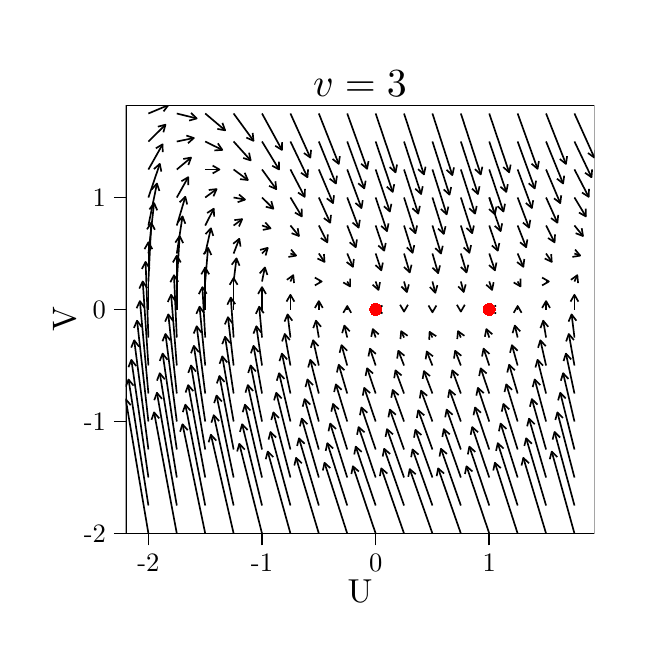
\begin{tikzpicture}[x=1pt,y=1pt]
\definecolor[named]{fillColor}{rgb}{1.00,1.00,1.00}
\path[use as bounding box,fill=fillColor,fill opacity=0.00] (0,0) rectangle (216.81,216.81);
\begin{scope}
\path[clip] (  0.00,  0.00) rectangle (216.81,216.81);
\definecolor[named]{drawColor}{rgb}{1.00,1.00,1.00}
\definecolor[named]{fillColor}{rgb}{1.00,1.00,1.00}

\path[draw=drawColor,line width= 0.6pt,line join=round,line cap=round,fill=fillColor] (  0.00,  0.00) rectangle (216.81,216.81);
\end{scope}
\begin{scope}
\path[clip] ( 35.42, 34.03) rectangle (204.76,188.82);
\definecolor[named]{fillColor}{rgb}{1.00,1.00,1.00}

\path[fill=fillColor] ( 35.42, 34.03) rectangle (204.76,188.82);
\definecolor[named]{fillColor}{rgb}{0.00,0.00,0.00}

\path[fill=fillColor,fill opacity=0.20] (166.79,155.44) circle (  0.11);

\path[fill=fillColor,fill opacity=0.20] ( 43.63, 34.03) circle (  0.11);

\path[fill=fillColor,fill opacity=0.20] ( 43.63, 44.15) circle (  0.11);

\path[fill=fillColor,fill opacity=0.20] ( 43.63, 54.27) circle (  0.11);

\path[fill=fillColor,fill opacity=0.20] ( 43.63, 64.39) circle (  0.11);

\path[fill=fillColor,fill opacity=0.20] ( 43.63, 74.50) circle (  0.11);

\path[fill=fillColor,fill opacity=0.20] ( 43.63, 84.62) circle (  0.11);

\path[fill=fillColor,fill opacity=0.20] ( 43.63, 94.74) circle (  0.11);

\path[fill=fillColor,fill opacity=0.20] ( 43.63,104.85) circle (  0.11);

\path[fill=fillColor,fill opacity=0.20] ( 43.63,114.97) circle (  0.11);

\path[fill=fillColor,fill opacity=0.20] ( 43.63,125.09) circle (  0.11);

\path[fill=fillColor,fill opacity=0.20] ( 43.63,135.20) circle (  0.11);

\path[fill=fillColor,fill opacity=0.20] ( 43.63,145.32) circle (  0.11);

\path[fill=fillColor,fill opacity=0.20] ( 43.63,155.44) circle (  0.11);

\path[fill=fillColor,fill opacity=0.20] ( 43.63,165.56) circle (  0.11);

\path[fill=fillColor,fill opacity=0.20] ( 43.63,175.67) circle (  0.11);

\path[fill=fillColor,fill opacity=0.20] ( 43.63,185.79) circle (  0.11);

\path[fill=fillColor,fill opacity=0.20] ( 53.89, 34.03) circle (  0.11);

\path[fill=fillColor,fill opacity=0.20] ( 53.89, 44.15) circle (  0.11);

\path[fill=fillColor,fill opacity=0.20] ( 53.89, 54.27) circle (  0.11);

\path[fill=fillColor,fill opacity=0.20] ( 53.89, 64.39) circle (  0.11);

\path[fill=fillColor,fill opacity=0.20] ( 53.89, 74.50) circle (  0.11);

\path[fill=fillColor,fill opacity=0.20] ( 53.89, 84.62) circle (  0.11);

\path[fill=fillColor,fill opacity=0.20] ( 53.89, 94.74) circle (  0.11);

\path[fill=fillColor,fill opacity=0.20] ( 53.89,104.85) circle (  0.11);

\path[fill=fillColor,fill opacity=0.20] ( 53.89,114.97) circle (  0.11);

\path[fill=fillColor,fill opacity=0.20] ( 53.89,125.09) circle (  0.11);

\path[fill=fillColor,fill opacity=0.20] ( 53.89,135.20) circle (  0.11);

\path[fill=fillColor,fill opacity=0.20] ( 53.89,145.32) circle (  0.11);

\path[fill=fillColor,fill opacity=0.20] ( 53.89,155.44) circle (  0.11);

\path[fill=fillColor,fill opacity=0.20] ( 53.89,165.56) circle (  0.11);

\path[fill=fillColor,fill opacity=0.20] ( 53.89,175.67) circle (  0.11);

\path[fill=fillColor,fill opacity=0.20] ( 53.89,185.79) circle (  0.11);

\path[fill=fillColor,fill opacity=0.20] ( 64.16, 34.03) circle (  0.11);

\path[fill=fillColor,fill opacity=0.20] ( 64.16, 44.15) circle (  0.11);

\path[fill=fillColor,fill opacity=0.20] ( 64.16, 54.27) circle (  0.11);

\path[fill=fillColor,fill opacity=0.20] ( 64.16, 64.39) circle (  0.11);

\path[fill=fillColor,fill opacity=0.20] ( 64.16, 74.50) circle (  0.11);

\path[fill=fillColor,fill opacity=0.20] ( 64.16, 84.62) circle (  0.11);

\path[fill=fillColor,fill opacity=0.20] ( 64.16, 94.74) circle (  0.11);

\path[fill=fillColor,fill opacity=0.20] ( 64.16,104.85) circle (  0.11);

\path[fill=fillColor,fill opacity=0.20] ( 64.16,114.97) circle (  0.11);

\path[fill=fillColor,fill opacity=0.20] ( 64.16,125.09) circle (  0.11);

\path[fill=fillColor,fill opacity=0.20] ( 64.16,135.20) circle (  0.11);

\path[fill=fillColor,fill opacity=0.20] ( 64.16,145.32) circle (  0.11);

\path[fill=fillColor,fill opacity=0.20] ( 64.16,155.44) circle (  0.11);

\path[fill=fillColor,fill opacity=0.20] ( 64.16,165.56) circle (  0.11);

\path[fill=fillColor,fill opacity=0.20] ( 64.16,175.67) circle (  0.11);

\path[fill=fillColor,fill opacity=0.20] ( 64.16,185.79) circle (  0.11);

\path[fill=fillColor,fill opacity=0.20] ( 74.42, 34.03) circle (  0.11);

\path[fill=fillColor,fill opacity=0.20] ( 74.42, 44.15) circle (  0.11);

\path[fill=fillColor,fill opacity=0.20] ( 74.42, 54.27) circle (  0.11);

\path[fill=fillColor,fill opacity=0.20] ( 74.42, 64.39) circle (  0.11);

\path[fill=fillColor,fill opacity=0.20] ( 74.42, 74.50) circle (  0.11);

\path[fill=fillColor,fill opacity=0.20] ( 74.42, 84.62) circle (  0.11);

\path[fill=fillColor,fill opacity=0.20] ( 74.42, 94.74) circle (  0.11);

\path[fill=fillColor,fill opacity=0.20] ( 74.42,104.85) circle (  0.11);

\path[fill=fillColor,fill opacity=0.20] ( 74.42,114.97) circle (  0.11);

\path[fill=fillColor,fill opacity=0.20] ( 74.42,125.09) circle (  0.11);

\path[fill=fillColor,fill opacity=0.20] ( 74.42,135.20) circle (  0.11);

\path[fill=fillColor,fill opacity=0.20] ( 74.42,145.32) circle (  0.11);

\path[fill=fillColor,fill opacity=0.20] ( 74.42,155.44) circle (  0.11);

\path[fill=fillColor,fill opacity=0.20] ( 74.42,165.56) circle (  0.11);

\path[fill=fillColor,fill opacity=0.20] ( 74.42,175.67) circle (  0.11);

\path[fill=fillColor,fill opacity=0.20] ( 74.42,185.79) circle (  0.11);

\path[fill=fillColor,fill opacity=0.20] ( 84.68, 34.03) circle (  0.11);

\path[fill=fillColor,fill opacity=0.20] ( 84.68, 44.15) circle (  0.11);

\path[fill=fillColor,fill opacity=0.20] ( 84.68, 54.27) circle (  0.11);

\path[fill=fillColor,fill opacity=0.20] ( 84.68, 64.39) circle (  0.11);

\path[fill=fillColor,fill opacity=0.20] ( 84.68, 74.50) circle (  0.11);

\path[fill=fillColor,fill opacity=0.20] ( 84.68, 84.62) circle (  0.11);

\path[fill=fillColor,fill opacity=0.20] ( 84.68, 94.74) circle (  0.11);

\path[fill=fillColor,fill opacity=0.20] ( 84.68,104.85) circle (  0.11);

\path[fill=fillColor,fill opacity=0.20] ( 84.68,114.97) circle (  0.11);

\path[fill=fillColor,fill opacity=0.20] ( 84.68,125.09) circle (  0.11);

\path[fill=fillColor,fill opacity=0.20] ( 84.68,135.20) circle (  0.11);

\path[fill=fillColor,fill opacity=0.20] ( 84.68,145.32) circle (  0.11);

\path[fill=fillColor,fill opacity=0.20] ( 84.68,155.44) circle (  0.11);

\path[fill=fillColor,fill opacity=0.20] ( 84.68,165.56) circle (  0.11);

\path[fill=fillColor,fill opacity=0.20] ( 84.68,175.67) circle (  0.11);

\path[fill=fillColor,fill opacity=0.20] ( 84.68,185.79) circle (  0.11);

\path[fill=fillColor,fill opacity=0.20] ( 94.95, 34.03) circle (  0.11);

\path[fill=fillColor,fill opacity=0.20] ( 94.95, 44.15) circle (  0.11);

\path[fill=fillColor,fill opacity=0.20] ( 94.95, 54.27) circle (  0.11);

\path[fill=fillColor,fill opacity=0.20] ( 94.95, 64.39) circle (  0.11);

\path[fill=fillColor,fill opacity=0.20] ( 94.95, 74.50) circle (  0.11);

\path[fill=fillColor,fill opacity=0.20] ( 94.95, 84.62) circle (  0.11);

\path[fill=fillColor,fill opacity=0.20] ( 94.95, 94.74) circle (  0.11);

\path[fill=fillColor,fill opacity=0.20] ( 94.95,104.85) circle (  0.11);

\path[fill=fillColor,fill opacity=0.20] ( 94.95,114.97) circle (  0.11);

\path[fill=fillColor,fill opacity=0.20] ( 94.95,125.09) circle (  0.11);

\path[fill=fillColor,fill opacity=0.20] ( 94.95,135.20) circle (  0.11);

\path[fill=fillColor,fill opacity=0.20] ( 94.95,145.32) circle (  0.11);

\path[fill=fillColor,fill opacity=0.20] ( 94.95,155.44) circle (  0.11);

\path[fill=fillColor,fill opacity=0.20] ( 94.95,165.56) circle (  0.11);

\path[fill=fillColor,fill opacity=0.20] ( 94.95,175.67) circle (  0.11);

\path[fill=fillColor,fill opacity=0.20] ( 94.95,185.79) circle (  0.11);

\path[fill=fillColor,fill opacity=0.20] (105.21, 34.03) circle (  0.11);

\path[fill=fillColor,fill opacity=0.20] (105.21, 44.15) circle (  0.11);

\path[fill=fillColor,fill opacity=0.20] (105.21, 54.27) circle (  0.11);

\path[fill=fillColor,fill opacity=0.20] (105.21, 64.39) circle (  0.11);

\path[fill=fillColor,fill opacity=0.20] (105.21, 74.50) circle (  0.11);

\path[fill=fillColor,fill opacity=0.20] (105.21, 84.62) circle (  0.11);

\path[fill=fillColor,fill opacity=0.20] (105.21, 94.74) circle (  0.11);

\path[fill=fillColor,fill opacity=0.20] (105.21,104.85) circle (  0.11);

\path[fill=fillColor,fill opacity=0.20] (105.21,114.97) circle (  0.11);

\path[fill=fillColor,fill opacity=0.20] (105.21,125.09) circle (  0.11);

\path[fill=fillColor,fill opacity=0.20] (105.21,135.20) circle (  0.11);

\path[fill=fillColor,fill opacity=0.20] (105.21,145.32) circle (  0.11);

\path[fill=fillColor,fill opacity=0.20] (105.21,155.44) circle (  0.11);

\path[fill=fillColor,fill opacity=0.20] (105.21,165.56) circle (  0.11);

\path[fill=fillColor,fill opacity=0.20] (105.21,175.67) circle (  0.11);

\path[fill=fillColor,fill opacity=0.20] (105.21,185.79) circle (  0.11);

\path[fill=fillColor,fill opacity=0.20] (115.47, 34.03) circle (  0.11);

\path[fill=fillColor,fill opacity=0.20] (115.47, 44.15) circle (  0.11);

\path[fill=fillColor,fill opacity=0.20] (115.47, 54.27) circle (  0.11);

\path[fill=fillColor,fill opacity=0.20] (115.47, 64.39) circle (  0.11);

\path[fill=fillColor,fill opacity=0.20] (115.47, 74.50) circle (  0.11);

\path[fill=fillColor,fill opacity=0.20] (115.47, 84.62) circle (  0.11);

\path[fill=fillColor,fill opacity=0.20] (115.47, 94.74) circle (  0.11);

\path[fill=fillColor,fill opacity=0.20] (115.47,104.85) circle (  0.11);

\path[fill=fillColor,fill opacity=0.20] (115.47,114.97) circle (  0.11);

\path[fill=fillColor,fill opacity=0.20] (115.47,125.09) circle (  0.11);

\path[fill=fillColor,fill opacity=0.20] (115.47,135.20) circle (  0.11);

\path[fill=fillColor,fill opacity=0.20] (115.47,145.32) circle (  0.11);

\path[fill=fillColor,fill opacity=0.20] (115.47,155.44) circle (  0.11);

\path[fill=fillColor,fill opacity=0.20] (115.47,165.56) circle (  0.11);

\path[fill=fillColor,fill opacity=0.20] (115.47,175.67) circle (  0.11);

\path[fill=fillColor,fill opacity=0.20] (115.47,185.79) circle (  0.11);

\path[fill=fillColor,fill opacity=0.20] (125.74, 34.03) circle (  0.11);

\path[fill=fillColor,fill opacity=0.20] (125.74, 44.15) circle (  0.11);

\path[fill=fillColor,fill opacity=0.20] (125.74, 54.27) circle (  0.11);

\path[fill=fillColor,fill opacity=0.20] (125.74, 64.39) circle (  0.11);

\path[fill=fillColor,fill opacity=0.20] (125.74, 74.50) circle (  0.11);

\path[fill=fillColor,fill opacity=0.20] (125.74, 84.62) circle (  0.11);

\path[fill=fillColor,fill opacity=0.20] (125.74, 94.74) circle (  0.11);

\path[fill=fillColor,fill opacity=0.20] (125.74,104.85) circle (  0.11);

\path[fill=fillColor,fill opacity=0.20] (125.74,114.97) circle (  0.11);

\path[fill=fillColor,fill opacity=0.20] (125.74,125.09) circle (  0.11);

\path[fill=fillColor,fill opacity=0.20] (125.74,135.20) circle (  0.11);

\path[fill=fillColor,fill opacity=0.20] (125.74,145.32) circle (  0.11);

\path[fill=fillColor,fill opacity=0.20] (125.74,155.44) circle (  0.11);

\path[fill=fillColor,fill opacity=0.20] (125.74,165.56) circle (  0.11);

\path[fill=fillColor,fill opacity=0.20] (125.74,175.67) circle (  0.11);

\path[fill=fillColor,fill opacity=0.20] (125.74,185.79) circle (  0.11);

\path[fill=fillColor,fill opacity=0.20] (136.00, 34.03) circle (  0.11);

\path[fill=fillColor,fill opacity=0.20] (136.00, 44.15) circle (  0.11);

\path[fill=fillColor,fill opacity=0.20] (136.00, 54.27) circle (  0.11);

\path[fill=fillColor,fill opacity=0.20] (136.00, 64.39) circle (  0.11);

\path[fill=fillColor,fill opacity=0.20] (136.00, 74.50) circle (  0.11);

\path[fill=fillColor,fill opacity=0.20] (136.00, 84.62) circle (  0.11);

\path[fill=fillColor,fill opacity=0.20] (136.00, 94.74) circle (  0.11);

\path[fill=fillColor,fill opacity=0.20] (136.00,104.85) circle (  0.11);

\path[fill=fillColor,fill opacity=0.20] (136.00,114.97) circle (  0.11);

\path[fill=fillColor,fill opacity=0.20] (136.00,125.09) circle (  0.11);

\path[fill=fillColor,fill opacity=0.20] (136.00,135.20) circle (  0.11);

\path[fill=fillColor,fill opacity=0.20] (136.00,145.32) circle (  0.11);

\path[fill=fillColor,fill opacity=0.20] (136.00,155.44) circle (  0.11);

\path[fill=fillColor,fill opacity=0.20] (136.00,165.56) circle (  0.11);

\path[fill=fillColor,fill opacity=0.20] (136.00,175.67) circle (  0.11);

\path[fill=fillColor,fill opacity=0.20] (136.00,185.79) circle (  0.11);

\path[fill=fillColor,fill opacity=0.20] (146.26, 34.03) circle (  0.11);

\path[fill=fillColor,fill opacity=0.20] (146.26, 44.15) circle (  0.11);

\path[fill=fillColor,fill opacity=0.20] (146.26, 54.27) circle (  0.11);

\path[fill=fillColor,fill opacity=0.20] (146.26, 64.39) circle (  0.11);

\path[fill=fillColor,fill opacity=0.20] (146.26, 74.50) circle (  0.11);

\path[fill=fillColor,fill opacity=0.20] (146.26, 84.62) circle (  0.11);

\path[fill=fillColor,fill opacity=0.20] (146.26, 94.74) circle (  0.11);

\path[fill=fillColor,fill opacity=0.20] (146.26,104.85) circle (  0.11);

\path[fill=fillColor,fill opacity=0.20] (146.26,114.97) circle (  0.11);

\path[fill=fillColor,fill opacity=0.20] (146.26,125.09) circle (  0.11);

\path[fill=fillColor,fill opacity=0.20] (146.26,135.20) circle (  0.11);

\path[fill=fillColor,fill opacity=0.20] (146.26,145.32) circle (  0.11);

\path[fill=fillColor,fill opacity=0.20] (146.26,155.44) circle (  0.11);

\path[fill=fillColor,fill opacity=0.20] (146.26,165.56) circle (  0.11);

\path[fill=fillColor,fill opacity=0.20] (146.26,175.67) circle (  0.11);

\path[fill=fillColor,fill opacity=0.20] (146.26,185.79) circle (  0.11);

\path[fill=fillColor,fill opacity=0.20] (156.53, 34.03) circle (  0.11);

\path[fill=fillColor,fill opacity=0.20] (156.53, 44.15) circle (  0.11);

\path[fill=fillColor,fill opacity=0.20] (156.53, 54.27) circle (  0.11);

\path[fill=fillColor,fill opacity=0.20] (156.53, 64.39) circle (  0.11);

\path[fill=fillColor,fill opacity=0.20] (156.53, 74.50) circle (  0.11);

\path[fill=fillColor,fill opacity=0.20] (156.53, 84.62) circle (  0.11);

\path[fill=fillColor,fill opacity=0.20] (156.53, 94.74) circle (  0.11);

\path[fill=fillColor,fill opacity=0.20] (156.53,104.85) circle (  0.11);

\path[fill=fillColor,fill opacity=0.20] (156.53,114.97) circle (  0.11);

\path[fill=fillColor,fill opacity=0.20] (156.53,125.09) circle (  0.11);

\path[fill=fillColor,fill opacity=0.20] (156.53,135.20) circle (  0.11);

\path[fill=fillColor,fill opacity=0.20] (156.53,145.32) circle (  0.11);

\path[fill=fillColor,fill opacity=0.20] (156.53,155.44) circle (  0.11);

\path[fill=fillColor,fill opacity=0.20] (156.53,165.56) circle (  0.11);

\path[fill=fillColor,fill opacity=0.20] (156.53,175.67) circle (  0.11);

\path[fill=fillColor,fill opacity=0.20] (156.53,185.79) circle (  0.11);

\path[fill=fillColor,fill opacity=0.20] (166.79, 34.03) circle (  0.11);

\path[fill=fillColor,fill opacity=0.20] (166.79, 44.15) circle (  0.11);

\path[fill=fillColor,fill opacity=0.20] (166.79, 54.27) circle (  0.11);

\path[fill=fillColor,fill opacity=0.20] (166.79, 64.39) circle (  0.11);

\path[fill=fillColor,fill opacity=0.20] (166.79, 74.50) circle (  0.11);

\path[fill=fillColor,fill opacity=0.20] (166.79, 84.62) circle (  0.11);

\path[fill=fillColor,fill opacity=0.20] (166.79, 94.74) circle (  0.11);

\path[fill=fillColor,fill opacity=0.20] (166.79,104.85) circle (  0.11);

\path[fill=fillColor,fill opacity=0.20] (166.79,114.97) circle (  0.11);

\path[fill=fillColor,fill opacity=0.20] (166.79,125.09) circle (  0.11);

\path[fill=fillColor,fill opacity=0.20] (166.79,135.20) circle (  0.11);

\path[fill=fillColor,fill opacity=0.20] (166.79,145.32) circle (  0.11);

\path[fill=fillColor,fill opacity=0.20] (166.79,155.44) circle (  0.11);

\path[fill=fillColor,fill opacity=0.20] (166.79,165.56) circle (  0.11);

\path[fill=fillColor,fill opacity=0.20] (166.79,175.67) circle (  0.11);

\path[fill=fillColor,fill opacity=0.20] (166.79,185.79) circle (  0.11);

\path[fill=fillColor,fill opacity=0.20] (177.05, 34.03) circle (  0.11);

\path[fill=fillColor,fill opacity=0.20] (177.05, 44.15) circle (  0.11);

\path[fill=fillColor,fill opacity=0.20] (177.05, 54.27) circle (  0.11);

\path[fill=fillColor,fill opacity=0.20] (177.05, 64.39) circle (  0.11);

\path[fill=fillColor,fill opacity=0.20] (177.05, 74.50) circle (  0.11);

\path[fill=fillColor,fill opacity=0.20] (177.05, 84.62) circle (  0.11);

\path[fill=fillColor,fill opacity=0.20] (177.05, 94.74) circle (  0.11);

\path[fill=fillColor,fill opacity=0.20] (177.05,104.85) circle (  0.11);

\path[fill=fillColor,fill opacity=0.20] (177.05,114.97) circle (  0.11);

\path[fill=fillColor,fill opacity=0.20] (177.05,125.09) circle (  0.11);

\path[fill=fillColor,fill opacity=0.20] (177.05,135.20) circle (  0.11);

\path[fill=fillColor,fill opacity=0.20] (177.05,145.32) circle (  0.11);

\path[fill=fillColor,fill opacity=0.20] (177.05,155.44) circle (  0.11);

\path[fill=fillColor,fill opacity=0.20] (177.05,165.56) circle (  0.11);

\path[fill=fillColor,fill opacity=0.20] (177.05,175.67) circle (  0.11);

\path[fill=fillColor,fill opacity=0.20] (177.05,185.79) circle (  0.11);

\path[fill=fillColor,fill opacity=0.20] (187.32, 34.03) circle (  0.11);

\path[fill=fillColor,fill opacity=0.20] (187.32, 44.15) circle (  0.11);

\path[fill=fillColor,fill opacity=0.20] (187.32, 54.27) circle (  0.11);

\path[fill=fillColor,fill opacity=0.20] (187.32, 64.39) circle (  0.11);

\path[fill=fillColor,fill opacity=0.20] (187.32, 74.50) circle (  0.11);

\path[fill=fillColor,fill opacity=0.20] (187.32, 84.62) circle (  0.11);

\path[fill=fillColor,fill opacity=0.20] (187.32, 94.74) circle (  0.11);

\path[fill=fillColor,fill opacity=0.20] (187.32,104.85) circle (  0.11);

\path[fill=fillColor,fill opacity=0.20] (187.32,114.97) circle (  0.11);

\path[fill=fillColor,fill opacity=0.20] (187.32,125.09) circle (  0.11);

\path[fill=fillColor,fill opacity=0.20] (187.32,135.20) circle (  0.11);

\path[fill=fillColor,fill opacity=0.20] (187.32,145.32) circle (  0.11);

\path[fill=fillColor,fill opacity=0.20] (187.32,155.44) circle (  0.11);

\path[fill=fillColor,fill opacity=0.20] (187.32,165.56) circle (  0.11);

\path[fill=fillColor,fill opacity=0.20] (187.32,175.67) circle (  0.11);

\path[fill=fillColor,fill opacity=0.20] (187.32,185.79) circle (  0.11);

\path[fill=fillColor,fill opacity=0.20] (197.58, 34.03) circle (  0.11);

\path[fill=fillColor,fill opacity=0.20] (197.58, 44.15) circle (  0.11);

\path[fill=fillColor,fill opacity=0.20] (197.58, 54.27) circle (  0.11);

\path[fill=fillColor,fill opacity=0.20] (197.58, 64.39) circle (  0.11);

\path[fill=fillColor,fill opacity=0.20] (197.58, 74.50) circle (  0.11);

\path[fill=fillColor,fill opacity=0.20] (197.58, 84.62) circle (  0.11);

\path[fill=fillColor,fill opacity=0.20] (197.58, 94.74) circle (  0.11);

\path[fill=fillColor,fill opacity=0.20] (197.58,104.85) circle (  0.11);

\path[fill=fillColor,fill opacity=0.20] (197.58,114.97) circle (  0.11);

\path[fill=fillColor,fill opacity=0.20] (197.58,125.09) circle (  0.11);

\path[fill=fillColor,fill opacity=0.20] (197.58,135.20) circle (  0.11);

\path[fill=fillColor,fill opacity=0.20] (197.58,145.32) circle (  0.11);

\path[fill=fillColor,fill opacity=0.20] (197.58,155.44) circle (  0.11);

\path[fill=fillColor,fill opacity=0.20] (197.58,165.56) circle (  0.11);

\path[fill=fillColor,fill opacity=0.20] (197.58,175.67) circle (  0.11);

\path[fill=fillColor,fill opacity=0.20] (197.58,185.79) circle (  0.11);
\definecolor[named]{drawColor}{rgb}{0.00,0.00,0.00}
\definecolor[named]{fillColor}{rgb}{0.00,0.00,0.00}

\path[draw=drawColor,line width= 0.6pt,line join=round,fill=fillColor] (166.79,155.44) -- (168.84,149.37);

\path[draw=drawColor,line width= 0.6pt,line join=round] (166.71,151.25) --
	(168.84,149.37) --
	(169.40,152.16);

\path[draw=drawColor,line width= 0.6pt,line join=round,fill=fillColor] ( 43.63, 34.03) -- ( 35.42, 82.60);

\path[draw=drawColor,line width= 0.6pt,line join=round] ( 37.23, 80.40) --
	( 35.42, 82.60) --
	( 34.43, 79.93);

\path[draw=drawColor,line width= 0.6pt,line join=round,fill=fillColor] ( 43.63, 44.15) -- ( 36.45, 89.68);

\path[draw=drawColor,line width= 0.6pt,line join=round] ( 38.24, 87.47) --
	( 36.45, 89.68) --
	( 35.43, 87.02);

\path[draw=drawColor,line width= 0.6pt,line join=round,fill=fillColor] ( 43.63, 54.27) -- ( 37.47, 96.76);

\path[draw=drawColor,line width= 0.6pt,line join=round] ( 39.23, 94.53) --
	( 37.47, 96.76) --
	( 36.42, 94.12);

\path[draw=drawColor,line width= 0.6pt,line join=round,fill=fillColor] ( 43.63, 64.39) -- ( 38.50,103.84);

\path[draw=drawColor,line width= 0.6pt,line join=round] ( 40.23,101.58) --
	( 38.50,103.84) --
	( 37.41,101.21);

\path[draw=drawColor,line width= 0.6pt,line join=round,fill=fillColor] ( 43.63, 74.50) -- ( 39.53,110.92);

\path[draw=drawColor,line width= 0.6pt,line join=round] ( 41.22,108.63) --
	( 39.53,110.92) --
	( 38.39,108.32);

\path[draw=drawColor,line width= 0.6pt,line join=round,fill=fillColor] ( 43.63, 84.62) -- ( 40.55,118.01);

\path[draw=drawColor,line width= 0.6pt,line join=round] ( 42.20,115.68) --
	( 40.55,118.01) --
	( 39.36,115.42);

\path[draw=drawColor,line width= 0.6pt,line join=round,fill=fillColor] ( 43.63, 94.74) -- ( 41.58,125.09);

\path[draw=drawColor,line width= 0.6pt,line join=round] ( 43.16,122.73) --
	( 41.58,125.09) --
	( 40.33,122.53);

\path[draw=drawColor,line width= 0.6pt,line join=round,fill=fillColor] ( 43.63,104.85) -- ( 42.61,132.17);

\path[draw=drawColor,line width= 0.6pt,line join=round] ( 44.12,129.76) --
	( 42.61,132.17) --
	( 41.28,129.65);

\path[draw=drawColor,line width= 0.6pt,line join=round,fill=fillColor] ( 43.63,114.97) -- ( 43.63,139.25);

\path[draw=drawColor,line width= 0.6pt,line join=round] ( 45.05,136.79) --
	( 43.63,139.25) --
	( 42.21,136.79);

\path[draw=drawColor,line width= 0.6pt,line join=round,fill=fillColor] ( 43.63,125.09) -- ( 44.66,146.33);

\path[draw=drawColor,line width= 0.6pt,line join=round] ( 45.96,143.80) --
	( 44.66,146.33) --
	( 43.12,143.94);

\path[draw=drawColor,line width= 0.6pt,line join=round,fill=fillColor] ( 43.63,135.20) -- ( 45.68,153.42);

\path[draw=drawColor,line width= 0.6pt,line join=round] ( 46.82,150.81) --
	( 45.68,153.42) --
	( 43.99,151.13);

\path[draw=drawColor,line width= 0.6pt,line join=round,fill=fillColor] ( 43.63,145.32) -- ( 46.71,160.50);

\path[draw=drawColor,line width= 0.6pt,line join=round] ( 47.61,157.80) --
	( 46.71,160.50) --
	( 44.83,158.37);

\path[draw=drawColor,line width= 0.6pt,line join=round,fill=fillColor] ( 43.63,155.44) -- ( 47.74,167.58);

\path[draw=drawColor,line width= 0.6pt,line join=round] ( 48.30,164.79) --
	( 47.74,167.58) --
	( 45.60,165.70);

\path[draw=drawColor,line width= 0.6pt,line join=round,fill=fillColor] ( 43.63,165.56) -- ( 48.76,174.66);

\path[draw=drawColor,line width= 0.6pt,line join=round] ( 48.79,171.82) --
	( 48.76,174.66) --
	( 46.31,173.21);

\path[draw=drawColor,line width= 0.6pt,line join=round,fill=fillColor] ( 43.63,175.67) -- ( 49.79,181.74);

\path[draw=drawColor,line width= 0.6pt,line join=round] ( 49.03,179.00) --
	( 49.79,181.74) --
	( 47.04,181.03);

\path[draw=drawColor,line width= 0.6pt,line join=round,fill=fillColor] ( 43.63,185.79) -- ( 50.82,188.82);

\path[draw=drawColor,line width= 0.6pt,line join=round] ( 49.10,186.56) --
	( 50.82,188.82) --
	( 47.99,189.18);

\path[draw=drawColor,line width= 0.6pt,line join=round,fill=fillColor] ( 53.89, 34.03) -- ( 45.68, 77.79);

\path[draw=drawColor,line width= 0.6pt,line join=round] ( 47.54, 75.63) --
	( 45.68, 77.79) --
	( 44.74, 75.11);

\path[draw=drawColor,line width= 0.6pt,line join=round,fill=fillColor] ( 53.89, 44.15) -- ( 46.71, 84.87);

\path[draw=drawColor,line width= 0.6pt,line join=round] ( 48.54, 82.69) --
	( 46.71, 84.87) --
	( 45.74, 82.20);

\path[draw=drawColor,line width= 0.6pt,line join=round,fill=fillColor] ( 53.89, 54.27) -- ( 47.74, 91.95);

\path[draw=drawColor,line width= 0.6pt,line join=round] ( 49.54, 89.75) --
	( 47.74, 91.95) --
	( 46.73, 89.29);

\path[draw=drawColor,line width= 0.6pt,line join=round,fill=fillColor] ( 53.89, 64.39) -- ( 48.76, 99.04);

\path[draw=drawColor,line width= 0.6pt,line join=round] ( 50.53, 96.81) --
	( 48.76, 99.04) --
	( 47.72, 96.39);

\path[draw=drawColor,line width= 0.6pt,line join=round,fill=fillColor] ( 53.89, 74.50) -- ( 49.79,106.12);

\path[draw=drawColor,line width= 0.6pt,line join=round] ( 51.52,103.86) --
	( 49.79,106.12) --
	( 48.70,103.49);

\path[draw=drawColor,line width= 0.6pt,line join=round,fill=fillColor] ( 53.89, 84.62) -- ( 50.82,113.20);

\path[draw=drawColor,line width= 0.6pt,line join=round] ( 52.49,110.90) --
	( 50.82,113.20) --
	( 49.67,110.60);

\path[draw=drawColor,line width= 0.6pt,line join=round,fill=fillColor] ( 53.89, 94.74) -- ( 51.84,120.28);

\path[draw=drawColor,line width= 0.6pt,line join=round] ( 53.46,117.94) --
	( 51.84,120.28) --
	( 50.62,117.71);

\path[draw=drawColor,line width= 0.6pt,line join=round,fill=fillColor] ( 53.89,104.85) -- ( 52.87,127.36);

\path[draw=drawColor,line width= 0.6pt,line join=round] ( 54.40,124.97) --
	( 52.87,127.36) --
	( 51.56,124.84);

\path[draw=drawColor,line width= 0.6pt,line join=round,fill=fillColor] ( 53.89,114.97) -- ( 53.89,134.45);

\path[draw=drawColor,line width= 0.6pt,line join=round] ( 55.32,131.98) --
	( 53.89,134.45) --
	( 52.47,131.98);

\path[draw=drawColor,line width= 0.6pt,line join=round,fill=fillColor] ( 53.89,125.09) -- ( 54.92,141.53);

\path[draw=drawColor,line width= 0.6pt,line join=round] ( 56.19,138.98) --
	( 54.92,141.53) --
	( 53.35,139.16);

\path[draw=drawColor,line width= 0.6pt,line join=round,fill=fillColor] ( 53.89,135.20) -- ( 55.95,148.61);

\path[draw=drawColor,line width= 0.6pt,line join=round] ( 56.98,145.96) --
	( 55.95,148.61) --
	( 54.17,146.39);

\path[draw=drawColor,line width= 0.6pt,line join=round,fill=fillColor] ( 53.89,145.32) -- ( 56.97,155.69);

\path[draw=drawColor,line width= 0.6pt,line join=round] ( 57.64,152.92) --
	( 56.97,155.69) --
	( 54.91,153.73);

\path[draw=drawColor,line width= 0.6pt,line join=round,fill=fillColor] ( 53.89,155.44) -- ( 58.00,162.77);

\path[draw=drawColor,line width= 0.6pt,line join=round] ( 58.04,159.93) --
	( 58.00,162.77) --
	( 55.56,161.32);

\path[draw=drawColor,line width= 0.6pt,line join=round,fill=fillColor] ( 53.89,165.56) -- ( 59.03,169.86);

\path[draw=drawColor,line width= 0.6pt,line join=round] ( 58.05,167.18) --
	( 59.03,169.86) --
	( 56.22,169.36);

\path[draw=drawColor,line width= 0.6pt,line join=round,fill=fillColor] ( 53.89,175.67) -- ( 60.05,176.94);

\path[draw=drawColor,line width= 0.6pt,line join=round] ( 57.93,175.05) --
	( 60.05,176.94) --
	( 57.35,177.84);

\path[draw=drawColor,line width= 0.6pt,line join=round,fill=fillColor] ( 53.89,185.79) -- ( 61.08,184.02);

\path[draw=drawColor,line width= 0.6pt,line join=round] ( 58.35,183.23) --
	( 61.08,184.02) --
	( 59.03,185.99);

\path[draw=drawColor,line width= 0.6pt,line join=round,fill=fillColor] ( 64.16, 34.03) -- ( 55.95, 73.49);

\path[draw=drawColor,line width= 0.6pt,line join=round] ( 57.84, 71.37) --
	( 55.95, 73.49) --
	( 55.06, 70.79);

\path[draw=drawColor,line width= 0.6pt,line join=round,fill=fillColor] ( 64.16, 44.15) -- ( 56.97, 80.57);

\path[draw=drawColor,line width= 0.6pt,line join=round] ( 58.85, 78.43) --
	( 56.97, 80.57) --
	( 56.05, 77.88);

\path[draw=drawColor,line width= 0.6pt,line join=round,fill=fillColor] ( 64.16, 54.27) -- ( 58.00, 87.65);

\path[draw=drawColor,line width= 0.6pt,line join=round] ( 59.85, 85.49) --
	( 58.00, 87.65) --
	( 57.05, 84.97);

\path[draw=drawColor,line width= 0.6pt,line join=round,fill=fillColor] ( 64.16, 64.39) -- ( 59.03, 94.74);

\path[draw=drawColor,line width= 0.6pt,line join=round] ( 60.84, 92.54) --
	( 59.03, 94.74) --
	( 58.03, 92.07);

\path[draw=drawColor,line width= 0.6pt,line join=round,fill=fillColor] ( 64.16, 74.50) -- ( 60.05,101.82);

\path[draw=drawColor,line width= 0.6pt,line join=round] ( 61.83, 99.59) --
	( 60.05,101.82) --
	( 59.01, 99.17);

\path[draw=drawColor,line width= 0.6pt,line join=round,fill=fillColor] ( 64.16, 84.62) -- ( 61.08,108.90);

\path[draw=drawColor,line width= 0.6pt,line join=round] ( 62.80,106.63) --
	( 61.08,108.90) --
	( 59.98,106.28);

\path[draw=drawColor,line width= 0.6pt,line join=round,fill=fillColor] ( 64.16, 94.74) -- ( 62.11,115.98);

\path[draw=drawColor,line width= 0.6pt,line join=round] ( 63.76,113.67) --
	( 62.11,115.98) --
	( 60.93,113.39);

\path[draw=drawColor,line width= 0.6pt,line join=round,fill=fillColor] ( 64.16,104.85) -- ( 63.13,123.06);

\path[draw=drawColor,line width= 0.6pt,line join=round] ( 64.69,120.68) --
	( 63.13,123.06) --
	( 61.85,120.52);

\path[draw=drawColor,line width= 0.6pt,line join=round,fill=fillColor] ( 64.16,114.97) -- ( 64.16,130.15);

\path[draw=drawColor,line width= 0.6pt,line join=round] ( 65.58,127.68) --
	( 64.16,130.15) --
	( 62.74,127.68);

\path[draw=drawColor,line width= 0.6pt,line join=round,fill=fillColor] ( 64.16,125.09) -- ( 65.18,137.23);

\path[draw=drawColor,line width= 0.6pt,line join=round] ( 66.39,134.65) --
	( 65.18,137.23) --
	( 63.56,134.89);

\path[draw=drawColor,line width= 0.6pt,line join=round,fill=fillColor] ( 64.16,135.20) -- ( 66.21,144.31);

\path[draw=drawColor,line width= 0.6pt,line join=round] ( 67.06,141.59) --
	( 66.21,144.31) --
	( 64.28,142.22);

\path[draw=drawColor,line width= 0.6pt,line join=round,fill=fillColor] ( 64.16,145.32) -- ( 67.24,151.39);

\path[draw=drawColor,line width= 0.6pt,line join=round] ( 67.39,148.55) --
	( 67.24,151.39) --
	( 64.85,149.84);

\path[draw=drawColor,line width= 0.6pt,line join=round,fill=fillColor] ( 64.16,155.44) -- ( 68.26,158.47);

\path[draw=drawColor,line width= 0.6pt,line join=round] ( 67.13,155.87) --
	( 68.26,158.47) --
	( 65.44,158.15);

\path[draw=drawColor,line width= 0.6pt,line join=round,fill=fillColor] ( 64.16,165.56) -- ( 69.29,165.56);

\path[draw=drawColor,line width= 0.6pt,line join=round] ( 66.83,164.13) --
	( 69.29,165.56) --
	( 66.83,166.98);

\path[draw=drawColor,line width= 0.6pt,line join=round,fill=fillColor] ( 64.16,175.67) -- ( 70.32,172.64);

\path[draw=drawColor,line width= 0.6pt,line join=round] ( 67.48,172.45) --
	( 70.32,172.64) --
	( 68.73,175.00);

\path[draw=drawColor,line width= 0.6pt,line join=round,fill=fillColor] ( 64.16,185.79) -- ( 71.34,179.72);

\path[draw=drawColor,line width= 0.6pt,line join=round] ( 68.54,180.22) --
	( 71.34,179.72) --
	( 70.38,182.40);

\path[draw=drawColor,line width= 0.6pt,line join=round,fill=fillColor] ( 74.42, 34.03) -- ( 66.21, 69.70);

\path[draw=drawColor,line width= 0.6pt,line join=round] ( 68.15, 67.61) --
	( 66.21, 69.70) --
	( 65.38, 66.98);

\path[draw=drawColor,line width= 0.6pt,line join=round,fill=fillColor] ( 74.42, 44.15) -- ( 67.24, 76.78);

\path[draw=drawColor,line width= 0.6pt,line join=round] ( 69.16, 74.68) --
	( 67.24, 76.78) --
	( 66.38, 74.07);

\path[draw=drawColor,line width= 0.6pt,line join=round,fill=fillColor] ( 74.42, 54.27) -- ( 68.26, 83.86);

\path[draw=drawColor,line width= 0.6pt,line join=round] ( 70.16, 81.74) --
	( 68.26, 83.86) --
	( 67.37, 81.16);

\path[draw=drawColor,line width= 0.6pt,line join=round,fill=fillColor] ( 74.42, 64.39) -- ( 69.29, 90.94);

\path[draw=drawColor,line width= 0.6pt,line join=round] ( 71.15, 88.79) --
	( 69.29, 90.94) --
	( 68.36, 88.25);

\path[draw=drawColor,line width= 0.6pt,line join=round,fill=fillColor] ( 74.42, 74.50) -- ( 70.32, 98.02);

\path[draw=drawColor,line width= 0.6pt,line join=round] ( 72.14, 95.84) --
	( 70.32, 98.02) --
	( 69.34, 95.35);

\path[draw=drawColor,line width= 0.6pt,line join=round,fill=fillColor] ( 74.42, 84.62) -- ( 71.34,105.11);

\path[draw=drawColor,line width= 0.6pt,line join=round] ( 73.12,102.88) --
	( 71.34,105.11) --
	( 70.30,102.46);

\path[draw=drawColor,line width= 0.6pt,line join=round,fill=fillColor] ( 74.42, 94.74) -- ( 72.37,112.19);

\path[draw=drawColor,line width= 0.6pt,line join=round] ( 74.07,109.91) --
	( 72.37,112.19) --
	( 71.24,109.58);

\path[draw=drawColor,line width= 0.6pt,line join=round,fill=fillColor] ( 74.42,104.85) -- ( 73.40,119.27);

\path[draw=drawColor,line width= 0.6pt,line join=round] ( 74.99,116.91) --
	( 73.40,119.27) --
	( 72.15,116.71);

\path[draw=drawColor,line width= 0.6pt,line join=round,fill=fillColor] ( 74.42,114.97) -- ( 74.42,126.35);

\path[draw=drawColor,line width= 0.6pt,line join=round] ( 75.84,123.89) --
	( 74.42,126.35) --
	( 73.00,123.89);

\path[draw=drawColor,line width= 0.6pt,line join=round,fill=fillColor] ( 74.42,125.09) -- ( 75.45,133.43);

\path[draw=drawColor,line width= 0.6pt,line join=round] ( 76.56,130.81) --
	( 75.45,133.43) --
	( 73.73,131.16);

\path[draw=drawColor,line width= 0.6pt,line join=round,fill=fillColor] ( 74.42,135.20) -- ( 76.47,140.52);

\path[draw=drawColor,line width= 0.6pt,line join=round] ( 76.91,137.70) --
	( 76.47,140.52) --
	( 74.26,138.73);

\path[draw=drawColor,line width= 0.6pt,line join=round,fill=fillColor] ( 74.42,145.32) -- ( 77.50,147.60);

\path[draw=drawColor,line width= 0.6pt,line join=round] ( 76.36,144.99) --
	( 77.50,147.60) --
	( 74.67,147.28);

\path[draw=drawColor,line width= 0.6pt,line join=round,fill=fillColor] ( 74.42,155.44) -- ( 78.53,154.68);

\path[draw=drawColor,line width= 0.6pt,line join=round] ( 75.85,153.73) --
	( 78.53,154.68) --
	( 76.36,156.53);

\path[draw=drawColor,line width= 0.6pt,line join=round,fill=fillColor] ( 74.42,165.56) -- ( 79.55,161.76);

\path[draw=drawColor,line width= 0.6pt,line join=round] ( 76.73,162.08) --
	( 79.55,161.76) --
	( 78.42,164.37);

\path[draw=drawColor,line width= 0.6pt,line join=round,fill=fillColor] ( 74.42,175.67) -- ( 80.58,168.84);

\path[draw=drawColor,line width= 0.6pt,line join=round] ( 77.87,169.72) --
	( 80.58,168.84) --
	( 79.99,171.63);

\path[draw=drawColor,line width= 0.6pt,line join=round,fill=fillColor] ( 74.42,185.79) -- ( 81.61,175.93);

\path[draw=drawColor,line width= 0.6pt,line join=round] ( 79.01,177.08) --
	( 81.61,175.93) --
	( 81.30,178.76);

\path[draw=drawColor,line width= 0.6pt,line join=round,fill=fillColor] ( 84.68, 34.03) -- ( 76.47, 66.41);

\path[draw=drawColor,line width= 0.6pt,line join=round] ( 78.46, 64.37) --
	( 76.47, 66.41) --
	( 75.70, 63.67);

\path[draw=drawColor,line width= 0.6pt,line join=round,fill=fillColor] ( 84.68, 44.15) -- ( 77.50, 73.49);

\path[draw=drawColor,line width= 0.6pt,line join=round] ( 79.47, 71.44) --
	( 77.50, 73.49) --
	( 76.70, 70.76);

\path[draw=drawColor,line width= 0.6pt,line join=round,fill=fillColor] ( 84.68, 54.27) -- ( 78.53, 80.57);

\path[draw=drawColor,line width= 0.6pt,line join=round] ( 80.47, 78.50) --
	( 78.53, 80.57) --
	( 77.70, 77.85);

\path[draw=drawColor,line width= 0.6pt,line join=round,fill=fillColor] ( 84.68, 64.39) -- ( 79.55, 87.65);

\path[draw=drawColor,line width= 0.6pt,line join=round] ( 81.47, 85.55) --
	( 79.55, 87.65) --
	( 78.69, 84.94);

\path[draw=drawColor,line width= 0.6pt,line join=round,fill=fillColor] ( 84.68, 74.50) -- ( 80.58, 94.74);

\path[draw=drawColor,line width= 0.6pt,line join=round] ( 82.46, 92.60) --
	( 80.58, 94.74) --
	( 79.68, 92.04);

\path[draw=drawColor,line width= 0.6pt,line join=round,fill=fillColor] ( 84.68, 84.62) -- ( 81.61,101.82);

\path[draw=drawColor,line width= 0.6pt,line join=round] ( 83.44, 99.64) --
	( 81.61,101.82) --
	( 80.64, 99.14);

\path[draw=drawColor,line width= 0.6pt,line join=round,fill=fillColor] ( 84.68, 94.74) -- ( 82.63,108.90);

\path[draw=drawColor,line width= 0.6pt,line join=round] ( 84.39,106.67) --
	( 82.63,108.90) --
	( 81.58,106.26);

\path[draw=drawColor,line width= 0.6pt,line join=round,fill=fillColor] ( 84.68,104.85) -- ( 83.66,115.98);

\path[draw=drawColor,line width= 0.6pt,line join=round] ( 85.30,113.66) --
	( 83.66,115.98) --
	( 82.47,113.40);

\path[draw=drawColor,line width= 0.6pt,line join=round,fill=fillColor] ( 84.68,114.97) -- ( 84.68,123.06);

\path[draw=drawColor,line width= 0.6pt,line join=round] ( 86.11,120.60) --
	( 84.68,123.06) --
	( 83.26,120.60);

\path[draw=drawColor,line width= 0.6pt,line join=round,fill=fillColor] ( 84.68,125.09) -- ( 85.71,130.15);

\path[draw=drawColor,line width= 0.6pt,line join=round] ( 86.62,127.45) --
	( 85.71,130.15) --
	( 83.83,128.01);

\path[draw=drawColor,line width= 0.6pt,line join=round,fill=fillColor] ( 84.68,135.20) -- ( 86.74,137.23);

\path[draw=drawColor,line width= 0.6pt,line join=round] ( 85.98,134.49) --
	( 86.74,137.23) --
	( 83.98,136.51);

\path[draw=drawColor,line width= 0.6pt,line join=round,fill=fillColor] ( 84.68,145.32) -- ( 87.76,144.31);

\path[draw=drawColor,line width= 0.6pt,line join=round] ( 84.98,143.73) --
	( 87.76,144.31) --
	( 85.87,146.43);

\path[draw=drawColor,line width= 0.6pt,line join=round,fill=fillColor] ( 84.68,155.44) -- ( 88.79,151.39);

\path[draw=drawColor,line width= 0.6pt,line join=round] ( 86.04,152.11) --
	( 88.79,151.39) --
	( 88.03,154.13);

\path[draw=drawColor,line width= 0.6pt,line join=round,fill=fillColor] ( 84.68,165.56) -- ( 89.82,158.47);

\path[draw=drawColor,line width= 0.6pt,line join=round] ( 87.22,159.63) --
	( 89.82,158.47) --
	( 89.52,161.30);

\path[draw=drawColor,line width= 0.6pt,line join=round,fill=fillColor] ( 84.68,175.67) -- ( 90.84,165.56);

\path[draw=drawColor,line width= 0.6pt,line join=round] ( 88.35,166.92) --
	( 90.84,165.56) --
	( 90.78,168.40);

\path[draw=drawColor,line width= 0.6pt,line join=round,fill=fillColor] ( 84.68,185.79) -- ( 91.87,172.64);

\path[draw=drawColor,line width= 0.6pt,line join=round] ( 89.44,174.12) --
	( 91.87,172.64) --
	( 91.94,175.48);

\path[draw=drawColor,line width= 0.6pt,line join=round,fill=fillColor] ( 94.95, 34.03) -- ( 86.74, 63.63);

\path[draw=drawColor,line width= 0.6pt,line join=round] ( 88.77, 61.63) --
	( 86.74, 63.63) --
	( 86.03, 60.87);

\path[draw=drawColor,line width= 0.6pt,line join=round,fill=fillColor] ( 94.95, 44.15) -- ( 87.76, 70.71);

\path[draw=drawColor,line width= 0.6pt,line join=round] ( 89.78, 68.70) --
	( 87.76, 70.71) --
	( 87.03, 67.96);

\path[draw=drawColor,line width= 0.6pt,line join=round,fill=fillColor] ( 94.95, 54.27) -- ( 88.79, 77.79);

\path[draw=drawColor,line width= 0.6pt,line join=round] ( 90.79, 75.77) --
	( 88.79, 77.79) --
	( 88.04, 75.05);

\path[draw=drawColor,line width= 0.6pt,line join=round,fill=fillColor] ( 94.95, 64.39) -- ( 89.82, 84.87);

\path[draw=drawColor,line width= 0.6pt,line join=round] ( 91.80, 82.83) --
	( 89.82, 84.87) --
	( 89.03, 82.14);

\path[draw=drawColor,line width= 0.6pt,line join=round,fill=fillColor] ( 94.95, 74.50) -- ( 90.84, 91.95);

\path[draw=drawColor,line width= 0.6pt,line join=round] ( 92.79, 89.88) --
	( 90.84, 91.95) --
	( 90.02, 89.23);

\path[draw=drawColor,line width= 0.6pt,line join=round,fill=fillColor] ( 94.95, 84.62) -- ( 91.87, 99.04);

\path[draw=drawColor,line width= 0.6pt,line join=round] ( 93.77, 96.92) --
	( 91.87, 99.04) --
	( 90.99, 96.33);

\path[draw=drawColor,line width= 0.6pt,line join=round,fill=fillColor] ( 94.95, 94.74) -- ( 92.90,106.12);

\path[draw=drawColor,line width= 0.6pt,line join=round] ( 94.73,103.95) --
	( 92.90,106.12) --
	( 91.93,103.44);

\path[draw=drawColor,line width= 0.6pt,line join=round,fill=fillColor] ( 94.95,104.85) -- ( 93.92,113.20);

\path[draw=drawColor,line width= 0.6pt,line join=round] ( 95.63,110.93) --
	( 93.92,113.20) --
	( 92.81,110.58);

\path[draw=drawColor,line width= 0.6pt,line join=round,fill=fillColor] ( 94.95,114.97) -- ( 94.95,120.28);

\path[draw=drawColor,line width= 0.6pt,line join=round] ( 96.37,117.82) --
	( 94.95,120.28) --
	( 93.53,117.82);

\path[draw=drawColor,line width= 0.6pt,line join=round,fill=fillColor] ( 94.95,125.09) -- ( 95.97,127.36);

\path[draw=drawColor,line width= 0.6pt,line join=round] ( 96.26,124.53) --
	( 95.97,127.36) --
	( 93.66,125.70);

\path[draw=drawColor,line width= 0.6pt,line join=round,fill=fillColor] ( 94.95,135.20) -- ( 97.00,134.45);

\path[draw=drawColor,line width= 0.6pt,line join=round] ( 94.20,133.97) --
	( 97.00,134.45) --
	( 95.18,136.63);

\path[draw=drawColor,line width= 0.6pt,line join=round,fill=fillColor] ( 94.95,145.32) -- ( 98.03,141.53);

\path[draw=drawColor,line width= 0.6pt,line join=round] ( 95.37,142.54) --
	( 98.03,141.53) --
	( 97.58,144.34);

\path[draw=drawColor,line width= 0.6pt,line join=round,fill=fillColor] ( 94.95,155.44) -- ( 99.05,148.61);

\path[draw=drawColor,line width= 0.6pt,line join=round] ( 96.56,149.99) --
	( 99.05,148.61) --
	( 99.00,151.45);

\path[draw=drawColor,line width= 0.6pt,line join=round,fill=fillColor] ( 94.95,165.56) -- (100.08,155.69);

\path[draw=drawColor,line width= 0.6pt,line join=round] ( 97.68,157.22) --
	(100.08,155.69) --
	(100.20,158.53);

\path[draw=drawColor,line width= 0.6pt,line join=round,fill=fillColor] ( 94.95,175.67) -- (101.11,162.77);

\path[draw=drawColor,line width= 0.6pt,line join=round] ( 98.76,164.38) --
	(101.11,162.77) --
	(101.33,165.61);

\path[draw=drawColor,line width= 0.6pt,line join=round,fill=fillColor] ( 94.95,185.79) -- (102.13,169.86);

\path[draw=drawColor,line width= 0.6pt,line join=round] ( 99.82,171.52) --
	(102.13,169.86) --
	(102.42,172.69);

\path[draw=drawColor,line width= 0.6pt,line join=round,fill=fillColor] (105.21, 34.03) -- ( 97.00, 61.35);

\path[draw=drawColor,line width= 0.6pt,line join=round] ( 99.07, 59.40) --
	( 97.00, 61.35) --
	( 96.35, 58.58);

\path[draw=drawColor,line width= 0.6pt,line join=round,fill=fillColor] (105.21, 44.15) -- ( 98.03, 68.43);

\path[draw=drawColor,line width= 0.6pt,line join=round] (100.09, 66.47) --
	( 98.03, 68.43) --
	( 97.36, 65.67);

\path[draw=drawColor,line width= 0.6pt,line join=round,fill=fillColor] (105.21, 54.27) -- ( 99.05, 75.51);

\path[draw=drawColor,line width= 0.6pt,line join=round] (101.11, 73.54) --
	( 99.05, 75.51) --
	( 98.37, 72.75);

\path[draw=drawColor,line width= 0.6pt,line join=round,fill=fillColor] (105.21, 64.39) -- (100.08, 82.60);

\path[draw=drawColor,line width= 0.6pt,line join=round] (102.12, 80.61) --
	(100.08, 82.60) --
	( 99.38, 79.84);

\path[draw=drawColor,line width= 0.6pt,line join=round,fill=fillColor] (105.21, 74.50) -- (101.11, 89.68);

\path[draw=drawColor,line width= 0.6pt,line join=round] (103.12, 87.67) --
	(101.11, 89.68) --
	(100.38, 86.93);

\path[draw=drawColor,line width= 0.6pt,line join=round,fill=fillColor] (105.21, 84.62) -- (102.13, 96.76);

\path[draw=drawColor,line width= 0.6pt,line join=round] (104.12, 94.72) --
	(102.13, 96.76) --
	(101.36, 94.02);

\path[draw=drawColor,line width= 0.6pt,line join=round,fill=fillColor] (105.21, 94.74) -- (103.16,103.84);

\path[draw=drawColor,line width= 0.6pt,line join=round] (105.09,101.75) --
	(103.16,103.84) --
	(102.31,101.13);

\path[draw=drawColor,line width= 0.6pt,line join=round,fill=fillColor] (105.21,104.85) -- (104.18,110.92);

\path[draw=drawColor,line width= 0.6pt,line join=round] (106.00,108.73) --
	(104.18,110.92) --
	(103.19,108.26);

\path[draw=drawColor,line width= 0.6pt,line join=round,fill=fillColor] (105.21,114.97) -- (105.21,118.01);

\path[draw=drawColor,line width= 0.6pt,line join=round] (106.63,115.54) --
	(105.21,118.01) --
	(103.79,115.54);

\path[draw=drawColor,line width= 0.6pt,line join=round,fill=fillColor] (105.21,125.09) -- (106.24,125.09);

\path[draw=drawColor,line width= 0.6pt,line join=round] (103.77,123.67) --
	(106.24,125.09) --
	(103.77,126.51);

\path[draw=drawColor,line width= 0.6pt,line join=round,fill=fillColor] (105.21,135.20) -- (107.26,132.17);

\path[draw=drawColor,line width= 0.6pt,line join=round] (104.71,133.41) --
	(107.26,132.17) --
	(107.06,135.01);

\path[draw=drawColor,line width= 0.6pt,line join=round,fill=fillColor] (105.21,145.32) -- (108.29,139.25);

\path[draw=drawColor,line width= 0.6pt,line join=round] (105.91,140.81) --
	(108.29,139.25) --
	(108.44,142.09);

\path[draw=drawColor,line width= 0.6pt,line join=round,fill=fillColor] (105.21,155.44) -- (109.32,146.33);

\path[draw=drawColor,line width= 0.6pt,line join=round] (107.01,148.00) --
	(109.32,146.33) --
	(109.60,149.16);

\path[draw=drawColor,line width= 0.6pt,line join=round,fill=fillColor] (105.21,165.56) -- (110.34,153.42);

\path[draw=drawColor,line width= 0.6pt,line join=round] (108.07,155.13) --
	(110.34,153.42) --
	(110.69,156.24);

\path[draw=drawColor,line width= 0.6pt,line join=round,fill=fillColor] (105.21,175.67) -- (111.37,160.50);

\path[draw=drawColor,line width= 0.6pt,line join=round] (109.12,162.25) --
	(111.37,160.50) --
	(111.76,163.32);

\path[draw=drawColor,line width= 0.6pt,line join=round,fill=fillColor] (105.21,185.79) -- (112.40,167.58);

\path[draw=drawColor,line width= 0.6pt,line join=round] (110.17,169.35) --
	(112.40,167.58) --
	(112.81,170.39);

\path[draw=drawColor,line width= 0.6pt,line join=round,fill=fillColor] (115.47, 34.03) -- (107.26, 59.58);

\path[draw=drawColor,line width= 0.6pt,line join=round] (109.37, 57.67) --
	(107.26, 59.58) --
	(106.66, 56.80);

\path[draw=drawColor,line width= 0.6pt,line join=round,fill=fillColor] (115.47, 44.15) -- (108.29, 66.66);

\path[draw=drawColor,line width= 0.6pt,line join=round] (110.39, 64.75) --
	(108.29, 66.66) --
	(107.68, 63.88);

\path[draw=drawColor,line width= 0.6pt,line join=round,fill=fillColor] (115.47, 54.27) -- (109.32, 73.74);

\path[draw=drawColor,line width= 0.6pt,line join=round] (111.42, 71.82) --
	(109.32, 73.74) --
	(108.70, 70.97);

\path[draw=drawColor,line width= 0.6pt,line join=round,fill=fillColor] (115.47, 64.39) -- (110.34, 80.83);

\path[draw=drawColor,line width= 0.6pt,line join=round] (112.44, 78.90) --
	(110.34, 80.83) --
	(109.72, 78.05);

\path[draw=drawColor,line width= 0.6pt,line join=round,fill=fillColor] (115.47, 74.50) -- (111.37, 87.91);

\path[draw=drawColor,line width= 0.6pt,line join=round] (113.45, 85.97) --
	(111.37, 87.91) --
	(110.73, 85.14);

\path[draw=drawColor,line width= 0.6pt,line join=round,fill=fillColor] (115.47, 84.62) -- (112.40, 94.99);

\path[draw=drawColor,line width= 0.6pt,line join=round] (114.46, 93.03) --
	(112.40, 94.99) --
	(111.73, 92.22);

\path[draw=drawColor,line width= 0.6pt,line join=round,fill=fillColor] (115.47, 94.74) -- (113.42,102.07);

\path[draw=drawColor,line width= 0.6pt,line join=round] (115.46,100.08) --
	(113.42,102.07) --
	(112.72, 99.32);

\path[draw=drawColor,line width= 0.6pt,line join=round,fill=fillColor] (115.47,104.85) -- (114.45,109.15);

\path[draw=drawColor,line width= 0.6pt,line join=round] (116.40,107.09) --
	(114.45,109.15) --
	(113.64,106.43);

\path[draw=drawColor,line width= 0.6pt,line join=round,fill=fillColor] (115.47,114.97) -- (115.47,116.24);

\path[draw=drawColor,line width= 0.6pt,line join=round] (116.90,113.77) --
	(115.47,116.24) --
	(114.05,113.77);

\path[draw=drawColor,line width= 0.6pt,line join=round,fill=fillColor] (115.47,125.09) -- (116.50,123.32);

\path[draw=drawColor,line width= 0.6pt,line join=round] (114.03,124.74) --
	(116.50,123.32) --
	(116.50,126.16);

\path[draw=drawColor,line width= 0.6pt,line join=round,fill=fillColor] (115.47,135.20) -- (117.53,130.40);

\path[draw=drawColor,line width= 0.6pt,line join=round] (115.25,132.11) --
	(117.53,130.40) --
	(117.87,133.22);

\path[draw=drawColor,line width= 0.6pt,line join=round,fill=fillColor] (115.47,145.32) -- (118.55,137.48);

\path[draw=drawColor,line width= 0.6pt,line join=round] (116.33,139.25) --
	(118.55,137.48) --
	(118.98,140.29);

\path[draw=drawColor,line width= 0.6pt,line join=round,fill=fillColor] (115.47,155.44) -- (119.58,144.56);

\path[draw=drawColor,line width= 0.6pt,line join=round] (117.38,146.37) --
	(119.58,144.56) --
	(120.04,147.37);

\path[draw=drawColor,line width= 0.6pt,line join=round,fill=fillColor] (115.47,165.56) -- (120.61,151.64);

\path[draw=drawColor,line width= 0.6pt,line join=round] (118.42,153.46) --
	(120.61,151.64) --
	(121.09,154.45);

\path[draw=drawColor,line width= 0.6pt,line join=round,fill=fillColor] (115.47,175.67) -- (121.63,158.73);

\path[draw=drawColor,line width= 0.6pt,line join=round] (119.45,160.56) --
	(121.63,158.73) --
	(122.13,161.53);

\path[draw=drawColor,line width= 0.6pt,line join=round,fill=fillColor] (115.47,185.79) -- (122.66,165.81);

\path[draw=drawColor,line width= 0.6pt,line join=round] (120.49,167.65) --
	(122.66,165.81) --
	(123.16,168.61);

\path[draw=drawColor,line width= 0.6pt,line join=round,fill=fillColor] (125.74, 34.03) -- (117.53, 58.32);

\path[draw=drawColor,line width= 0.6pt,line join=round] (119.66, 56.44) --
	(117.53, 58.32) --
	(116.97, 55.53);

\path[draw=drawColor,line width= 0.6pt,line join=round,fill=fillColor] (125.74, 44.15) -- (118.55, 65.40);

\path[draw=drawColor,line width= 0.6pt,line join=round] (120.69, 63.52) --
	(118.55, 65.40) --
	(118.00, 62.61);

\path[draw=drawColor,line width= 0.6pt,line join=round,fill=fillColor] (125.74, 54.27) -- (119.58, 72.48);

\path[draw=drawColor,line width= 0.6pt,line join=round] (121.72, 70.60) --
	(119.58, 72.48) --
	(119.02, 69.69);

\path[draw=drawColor,line width= 0.6pt,line join=round,fill=fillColor] (125.74, 64.39) -- (120.61, 79.56);

\path[draw=drawColor,line width= 0.6pt,line join=round] (122.74, 77.68) --
	(120.61, 79.56) --
	(120.05, 76.77);

\path[draw=drawColor,line width= 0.6pt,line join=round,fill=fillColor] (125.74, 74.50) -- (121.63, 86.64);

\path[draw=drawColor,line width= 0.6pt,line join=round] (123.77, 84.76) --
	(121.63, 86.64) --
	(121.07, 83.85);

\path[draw=drawColor,line width= 0.6pt,line join=round,fill=fillColor] (125.74, 84.62) -- (122.66, 93.72);

\path[draw=drawColor,line width= 0.6pt,line join=round] (124.80, 91.85) --
	(122.66, 93.72) --
	(122.10, 90.94);

\path[draw=drawColor,line width= 0.6pt,line join=round,fill=fillColor] (125.74, 94.74) -- (123.69,100.81);

\path[draw=drawColor,line width= 0.6pt,line join=round] (125.82, 98.93) --
	(123.69,100.81) --
	(123.13, 98.02);

\path[draw=drawColor,line width= 0.6pt,line join=round,fill=fillColor] (125.74,104.85) -- (124.71,107.89);

\path[draw=drawColor,line width= 0.6pt,line join=round] (126.85,106.01) --
	(124.71,107.89) --
	(124.15,105.10);

\path[draw=drawColor,line width= 0.6pt,line join=round,fill=fillColor] (125.74,114.97) -- (125.74,114.97);

\path[draw=drawColor,line width= 0.6pt,line join=round] (128.20,116.39) --
	(125.74,114.97) --
	(128.20,113.55);

\path[draw=drawColor,line width= 0.6pt,line join=round,fill=fillColor] (125.74,125.09) -- (126.76,122.05);

\path[draw=drawColor,line width= 0.6pt,line join=round] (124.63,123.93) --
	(126.76,122.05) --
	(127.32,124.84);

\path[draw=drawColor,line width= 0.6pt,line join=round,fill=fillColor] (125.74,135.20) -- (127.79,129.13);

\path[draw=drawColor,line width= 0.6pt,line join=round] (125.65,131.01) --
	(127.79,129.13) --
	(128.35,131.92);

\path[draw=drawColor,line width= 0.6pt,line join=round,fill=fillColor] (125.74,145.32) -- (128.82,136.22);

\path[draw=drawColor,line width= 0.6pt,line join=round] (126.68,138.09) --
	(128.82,136.22) --
	(129.38,139.01);

\path[draw=drawColor,line width= 0.6pt,line join=round,fill=fillColor] (125.74,155.44) -- (129.84,143.30);

\path[draw=drawColor,line width= 0.6pt,line join=round] (127.71,145.18) --
	(129.84,143.30) --
	(130.40,146.09);

\path[draw=drawColor,line width= 0.6pt,line join=round,fill=fillColor] (125.74,165.56) -- (130.87,150.38);

\path[draw=drawColor,line width= 0.6pt,line join=round] (128.73,152.26) --
	(130.87,150.38) --
	(131.43,153.17);

\path[draw=drawColor,line width= 0.6pt,line join=round,fill=fillColor] (125.74,175.67) -- (131.90,157.46);

\path[draw=drawColor,line width= 0.6pt,line join=round] (129.76,159.34) --
	(131.90,157.46) --
	(132.45,160.25);

\path[draw=drawColor,line width= 0.6pt,line join=round,fill=fillColor] (125.74,185.79) -- (132.92,164.54);

\path[draw=drawColor,line width= 0.6pt,line join=round] (130.79,166.42) --
	(132.92,164.54) --
	(133.48,167.33);

\path[draw=drawColor,line width= 0.6pt,line join=round,fill=fillColor] (136.00, 34.03) -- (127.79, 57.56);

\path[draw=drawColor,line width= 0.6pt,line join=round] (129.95, 55.70) --
	(127.79, 57.56) --
	(127.26, 54.76);

\path[draw=drawColor,line width= 0.6pt,line join=round,fill=fillColor] (136.00, 44.15) -- (128.82, 64.64);

\path[draw=drawColor,line width= 0.6pt,line join=round] (130.97, 62.78) --
	(128.82, 64.64) --
	(128.29, 61.84);

\path[draw=drawColor,line width= 0.6pt,line join=round,fill=fillColor] (136.00, 54.27) -- (129.84, 71.72);

\path[draw=drawColor,line width= 0.6pt,line join=round] (132.00, 69.87) --
	(129.84, 71.72) --
	(129.32, 68.92);

\path[draw=drawColor,line width= 0.6pt,line join=round,fill=fillColor] (136.00, 64.39) -- (130.87, 78.80);

\path[draw=drawColor,line width= 0.6pt,line join=round] (133.04, 76.96) --
	(130.87, 78.80) --
	(130.36, 76.00);

\path[draw=drawColor,line width= 0.6pt,line join=round,fill=fillColor] (136.00, 74.50) -- (131.90, 85.88);

\path[draw=drawColor,line width= 0.6pt,line join=round] (134.07, 84.05) --
	(131.90, 85.88) --
	(131.39, 83.08);

\path[draw=drawColor,line width= 0.6pt,line join=round,fill=fillColor] (136.00, 84.62) -- (132.92, 92.97);

\path[draw=drawColor,line width= 0.6pt,line join=round] (135.11, 91.15) --
	(132.92, 92.97) --
	(132.44, 90.16);

\path[draw=drawColor,line width= 0.6pt,line join=round,fill=fillColor] (136.00, 94.74) -- (133.95,100.05);

\path[draw=drawColor,line width= 0.6pt,line join=round] (136.16, 98.26) --
	(133.95,100.05) --
	(133.51, 97.24);

\path[draw=drawColor,line width= 0.6pt,line join=round,fill=fillColor] (136.00,104.85) -- (134.97,107.13);

\path[draw=drawColor,line width= 0.6pt,line join=round] (137.28,105.47) --
	(134.97,107.13) --
	(134.69,104.30);

\path[draw=drawColor,line width= 0.6pt,line join=round,fill=fillColor] (136.00,114.97) -- (136.00,114.21);

\path[draw=drawColor,line width= 0.6pt,line join=round] (134.58,116.68) --
	(136.00,114.21) --
	(137.42,116.68);

\path[draw=drawColor,line width= 0.6pt,line join=round,fill=fillColor] (136.00,125.09) -- (137.03,121.29);

\path[draw=drawColor,line width= 0.6pt,line join=round] (135.01,123.30) --
	(137.03,121.29) --
	(137.76,124.04);

\path[draw=drawColor,line width= 0.6pt,line join=round,fill=fillColor] (136.00,135.20) -- (138.05,128.38);

\path[draw=drawColor,line width= 0.6pt,line join=round] (135.98,130.33) --
	(138.05,128.38) --
	(138.71,131.15);

\path[draw=drawColor,line width= 0.6pt,line join=round,fill=fillColor] (136.00,145.32) -- (139.08,135.46);

\path[draw=drawColor,line width= 0.6pt,line join=round] (136.99,137.39) --
	(139.08,135.46) --
	(139.70,138.23);

\path[draw=drawColor,line width= 0.6pt,line join=round,fill=fillColor] (136.00,155.44) -- (140.11,142.54);

\path[draw=drawColor,line width= 0.6pt,line join=round] (138.00,144.46) --
	(140.11,142.54) --
	(140.71,145.32);

\path[draw=drawColor,line width= 0.6pt,line join=round,fill=fillColor] (136.00,165.56) -- (141.13,149.62);

\path[draw=drawColor,line width= 0.6pt,line join=round] (139.02,151.53) --
	(141.13,149.62) --
	(141.73,152.40);

\path[draw=drawColor,line width= 0.6pt,line join=round,fill=fillColor] (136.00,175.67) -- (142.16,156.70);

\path[draw=drawColor,line width= 0.6pt,line join=round] (140.05,158.61) --
	(142.16,156.70) --
	(142.75,159.49);

\path[draw=drawColor,line width= 0.6pt,line join=round,fill=fillColor] (136.00,185.79) -- (143.19,163.79);

\path[draw=drawColor,line width= 0.6pt,line join=round] (141.07,165.69) --
	(143.19,163.79) --
	(143.77,166.57);

\path[draw=drawColor,line width= 0.6pt,line join=round,fill=fillColor] (146.26, 34.03) -- (138.05, 57.30);

\path[draw=drawColor,line width= 0.6pt,line join=round] (140.22, 55.45) --
	(138.05, 57.30) --
	(137.53, 54.51);

\path[draw=drawColor,line width= 0.6pt,line join=round,fill=fillColor] (146.26, 44.15) -- (139.08, 64.39);

\path[draw=drawColor,line width= 0.6pt,line join=round] (141.25, 62.54) --
	(139.08, 64.39) --
	(138.56, 61.59);

\path[draw=drawColor,line width= 0.6pt,line join=round,fill=fillColor] (146.26, 54.27) -- (140.11, 71.47);

\path[draw=drawColor,line width= 0.6pt,line join=round] (142.28, 69.63) --
	(140.11, 71.47) --
	(139.60, 68.67);

\path[draw=drawColor,line width= 0.6pt,line join=round,fill=fillColor] (146.26, 64.39) -- (141.13, 78.55);

\path[draw=drawColor,line width= 0.6pt,line join=round] (143.31, 76.72) --
	(141.13, 78.55) --
	(140.63, 75.75);

\path[draw=drawColor,line width= 0.6pt,line join=round,fill=fillColor] (146.26, 74.50) -- (142.16, 85.63);

\path[draw=drawColor,line width= 0.6pt,line join=round] (144.35, 83.81) --
	(142.16, 85.63) --
	(141.68, 82.83);

\path[draw=drawColor,line width= 0.6pt,line join=round,fill=fillColor] (146.26, 84.62) -- (143.19, 92.71);

\path[draw=drawColor,line width= 0.6pt,line join=round] (145.39, 90.92) --
	(143.19, 92.71) --
	(142.73, 89.90);

\path[draw=drawColor,line width= 0.6pt,line join=round,fill=fillColor] (146.26, 94.74) -- (144.21, 99.80);

\path[draw=drawColor,line width= 0.6pt,line join=round] (146.46, 98.05) --
	(144.21, 99.80) --
	(143.82, 96.98);

\path[draw=drawColor,line width= 0.6pt,line join=round,fill=fillColor] (146.26,104.85) -- (145.24,106.88);

\path[draw=drawColor,line width= 0.6pt,line join=round] (147.62,105.32) --
	(145.24,106.88) --
	(145.08,104.04);

\path[draw=drawColor,line width= 0.6pt,line join=round,fill=fillColor] (146.26,114.97) -- (146.26,113.96);

\path[draw=drawColor,line width= 0.6pt,line join=round] (144.84,116.42) --
	(146.26,113.96) --
	(147.69,116.42);

\path[draw=drawColor,line width= 0.6pt,line join=round,fill=fillColor] (146.26,125.09) -- (147.29,121.04);

\path[draw=drawColor,line width= 0.6pt,line join=round] (145.31,123.08) --
	(147.29,121.04) --
	(148.06,123.78);

\path[draw=drawColor,line width= 0.6pt,line join=round,fill=fillColor] (146.26,135.20) -- (148.32,128.12);

\path[draw=drawColor,line width= 0.6pt,line join=round] (146.26,130.09) --
	(148.32,128.12) --
	(149.00,130.89);

\path[draw=drawColor,line width= 0.6pt,line join=round,fill=fillColor] (146.26,145.32) -- (149.34,135.20);

\path[draw=drawColor,line width= 0.6pt,line join=round] (147.26,137.15) --
	(149.34,135.20) --
	(149.99,137.98);

\path[draw=drawColor,line width= 0.6pt,line join=round,fill=fillColor] (146.26,155.44) -- (150.37,142.29);

\path[draw=drawColor,line width= 0.6pt,line join=round] (148.28,144.21) --
	(150.37,142.29) --
	(150.99,145.06);

\path[draw=drawColor,line width= 0.6pt,line join=round,fill=fillColor] (146.26,165.56) -- (151.40,149.37);

\path[draw=drawColor,line width= 0.6pt,line join=round] (149.30,151.29) --
	(151.40,149.37) --
	(152.01,152.15);

\path[draw=drawColor,line width= 0.6pt,line join=round,fill=fillColor] (146.26,175.67) -- (152.42,156.45);

\path[draw=drawColor,line width= 0.6pt,line join=round] (150.32,158.36) --
	(152.42,156.45) --
	(153.03,159.23);

\path[draw=drawColor,line width= 0.6pt,line join=round,fill=fillColor] (146.26,185.79) -- (153.45,163.53);

\path[draw=drawColor,line width= 0.6pt,line join=round] (151.34,165.44) --
	(153.45,163.53) --
	(154.05,166.31);

\path[draw=drawColor,line width= 0.6pt,line join=round,fill=fillColor] (156.53, 34.03) -- (148.32, 57.56);

\path[draw=drawColor,line width= 0.6pt,line join=round] (150.47, 55.70) --
	(148.32, 57.56) --
	(147.79, 54.76);

\path[draw=drawColor,line width= 0.6pt,line join=round,fill=fillColor] (156.53, 44.15) -- (149.34, 64.64);

\path[draw=drawColor,line width= 0.6pt,line join=round] (151.50, 62.78) --
	(149.34, 64.64) --
	(148.82, 61.84);

\path[draw=drawColor,line width= 0.6pt,line join=round,fill=fillColor] (156.53, 54.27) -- (150.37, 71.72);

\path[draw=drawColor,line width= 0.6pt,line join=round] (152.53, 69.87) --
	(150.37, 71.72) --
	(149.85, 68.92);

\path[draw=drawColor,line width= 0.6pt,line join=round,fill=fillColor] (156.53, 64.39) -- (151.40, 78.80);

\path[draw=drawColor,line width= 0.6pt,line join=round] (153.56, 76.96) --
	(151.40, 78.80) --
	(150.88, 76.00);

\path[draw=drawColor,line width= 0.6pt,line join=round,fill=fillColor] (156.53, 74.50) -- (152.42, 85.88);

\path[draw=drawColor,line width= 0.6pt,line join=round] (154.60, 84.05) --
	(152.42, 85.88) --
	(151.92, 83.08);

\path[draw=drawColor,line width= 0.6pt,line join=round,fill=fillColor] (156.53, 84.62) -- (153.45, 92.97);

\path[draw=drawColor,line width= 0.6pt,line join=round] (155.64, 91.15) --
	(153.45, 92.97) --
	(152.97, 90.16);

\path[draw=drawColor,line width= 0.6pt,line join=round,fill=fillColor] (156.53, 94.74) -- (154.47,100.05);

\path[draw=drawColor,line width= 0.6pt,line join=round] (156.69, 98.26) --
	(154.47,100.05) --
	(154.04, 97.24);

\path[draw=drawColor,line width= 0.6pt,line join=round,fill=fillColor] (156.53,104.85) -- (155.50,107.13);

\path[draw=drawColor,line width= 0.6pt,line join=round] (157.81,105.47) --
	(155.50,107.13) --
	(155.22,104.30);

\path[draw=drawColor,line width= 0.6pt,line join=round,fill=fillColor] (156.53,114.97) -- (156.53,114.21);

\path[draw=drawColor,line width= 0.6pt,line join=round] (155.10,116.68) --
	(156.53,114.21) --
	(157.95,116.68);

\path[draw=drawColor,line width= 0.6pt,line join=round,fill=fillColor] (156.53,125.09) -- (157.55,121.29);

\path[draw=drawColor,line width= 0.6pt,line join=round] (155.54,123.30) --
	(157.55,121.29) --
	(158.28,124.04);

\path[draw=drawColor,line width= 0.6pt,line join=round,fill=fillColor] (156.53,135.20) -- (158.58,128.38);

\path[draw=drawColor,line width= 0.6pt,line join=round] (156.51,130.33) --
	(158.58,128.38) --
	(159.23,131.15);

\path[draw=drawColor,line width= 0.6pt,line join=round,fill=fillColor] (156.53,145.32) -- (159.61,135.46);

\path[draw=drawColor,line width= 0.6pt,line join=round] (157.51,137.39) --
	(159.61,135.46) --
	(160.23,138.23);

\path[draw=drawColor,line width= 0.6pt,line join=round,fill=fillColor] (156.53,155.44) -- (160.63,142.54);

\path[draw=drawColor,line width= 0.6pt,line join=round] (158.53,144.46) --
	(160.63,142.54) --
	(161.24,145.32);

\path[draw=drawColor,line width= 0.6pt,line join=round,fill=fillColor] (156.53,165.56) -- (161.66,149.62);

\path[draw=drawColor,line width= 0.6pt,line join=round] (159.55,151.53) --
	(161.66,149.62) --
	(162.26,152.40);

\path[draw=drawColor,line width= 0.6pt,line join=round,fill=fillColor] (156.53,175.67) -- (162.69,156.70);

\path[draw=drawColor,line width= 0.6pt,line join=round] (160.57,158.61) --
	(162.69,156.70) --
	(163.28,159.49);

\path[draw=drawColor,line width= 0.6pt,line join=round,fill=fillColor] (156.53,185.79) -- (163.71,163.79);

\path[draw=drawColor,line width= 0.6pt,line join=round] (161.59,165.69) --
	(163.71,163.79) --
	(164.30,166.57);

\path[draw=drawColor,line width= 0.6pt,line join=round,fill=fillColor] (166.79, 34.03) -- (158.58, 58.32);

\path[draw=drawColor,line width= 0.6pt,line join=round] (160.72, 56.44) --
	(158.58, 58.32) --
	(158.02, 55.53);

\path[draw=drawColor,line width= 0.6pt,line join=round,fill=fillColor] (166.79, 44.15) -- (159.61, 65.40);

\path[draw=drawColor,line width= 0.6pt,line join=round] (161.74, 63.52) --
	(159.61, 65.40) --
	(159.05, 62.61);

\path[draw=drawColor,line width= 0.6pt,line join=round,fill=fillColor] (166.79, 54.27) -- (160.63, 72.48);

\path[draw=drawColor,line width= 0.6pt,line join=round] (162.77, 70.60) --
	(160.63, 72.48) --
	(160.07, 69.69);

\path[draw=drawColor,line width= 0.6pt,line join=round,fill=fillColor] (166.79, 64.39) -- (161.66, 79.56);

\path[draw=drawColor,line width= 0.6pt,line join=round] (163.80, 77.68) --
	(161.66, 79.56) --
	(161.10, 76.77);

\path[draw=drawColor,line width= 0.6pt,line join=round,fill=fillColor] (166.79, 74.50) -- (162.69, 86.64);

\path[draw=drawColor,line width= 0.6pt,line join=round] (164.82, 84.76) --
	(162.69, 86.64) --
	(162.13, 83.85);

\path[draw=drawColor,line width= 0.6pt,line join=round,fill=fillColor] (166.79, 84.62) -- (163.71, 93.72);

\path[draw=drawColor,line width= 0.6pt,line join=round] (165.85, 91.85) --
	(163.71, 93.72) --
	(163.15, 90.94);

\path[draw=drawColor,line width= 0.6pt,line join=round,fill=fillColor] (166.79, 94.74) -- (164.74,100.81);

\path[draw=drawColor,line width= 0.6pt,line join=round] (166.88, 98.93) --
	(164.74,100.81) --
	(164.18, 98.02);

\path[draw=drawColor,line width= 0.6pt,line join=round,fill=fillColor] (166.79,104.85) -- (165.76,107.89);

\path[draw=drawColor,line width= 0.6pt,line join=round] (167.90,106.01) --
	(165.76,107.89) --
	(165.21,105.10);

\path[draw=drawColor,line width= 0.6pt,line join=round,fill=fillColor] (166.79,114.97) -- (166.79,114.97);

\path[draw=drawColor,line width= 0.6pt,line join=round] (169.25,116.39) --
	(166.79,114.97) --
	(169.25,113.55);

\path[draw=drawColor,line width= 0.6pt,line join=round,fill=fillColor] (166.79,125.09) -- (167.82,122.05);

\path[draw=drawColor,line width= 0.6pt,line join=round] (165.68,123.93) --
	(167.82,122.05) --
	(168.38,124.84);

\path[draw=drawColor,line width= 0.6pt,line join=round,fill=fillColor] (166.79,135.20) -- (168.84,129.13);

\path[draw=drawColor,line width= 0.6pt,line join=round] (166.71,131.01) --
	(168.84,129.13) --
	(169.40,131.92);

\path[draw=drawColor,line width= 0.6pt,line join=round,fill=fillColor] (166.79,145.32) -- (169.87,136.22);

\path[draw=drawColor,line width= 0.6pt,line join=round] (167.73,138.09) --
	(169.87,136.22) --
	(170.43,139.01);

\path[draw=drawColor,line width= 0.6pt,line join=round,fill=fillColor] (166.79,155.44) -- (170.90,143.30);

\path[draw=drawColor,line width= 0.6pt,line join=round] (168.76,145.18) --
	(170.90,143.30) --
	(171.45,146.09);

\path[draw=drawColor,line width= 0.6pt,line join=round,fill=fillColor] (166.79,165.56) -- (171.92,150.38);

\path[draw=drawColor,line width= 0.6pt,line join=round] (169.79,152.26) --
	(171.92,150.38) --
	(172.48,153.17);

\path[draw=drawColor,line width= 0.6pt,line join=round,fill=fillColor] (166.79,175.67) -- (172.95,157.46);

\path[draw=drawColor,line width= 0.6pt,line join=round] (170.81,159.34) --
	(172.95,157.46) --
	(173.51,160.25);

\path[draw=drawColor,line width= 0.6pt,line join=round,fill=fillColor] (166.79,185.79) -- (173.98,164.54);

\path[draw=drawColor,line width= 0.6pt,line join=round] (171.84,166.42) --
	(173.98,164.54) --
	(174.53,167.33);

\path[draw=drawColor,line width= 0.6pt,line join=round,fill=fillColor] (177.05, 34.03) -- (168.84, 59.58);

\path[draw=drawColor,line width= 0.6pt,line join=round] (170.95, 57.67) --
	(168.84, 59.58) --
	(168.24, 56.80);

\path[draw=drawColor,line width= 0.6pt,line join=round,fill=fillColor] (177.05, 44.15) -- (169.87, 66.66);

\path[draw=drawColor,line width= 0.6pt,line join=round] (171.97, 64.75) --
	(169.87, 66.66) --
	(169.26, 63.88);

\path[draw=drawColor,line width= 0.6pt,line join=round,fill=fillColor] (177.05, 54.27) -- (170.90, 73.74);

\path[draw=drawColor,line width= 0.6pt,line join=round] (173.00, 71.82) --
	(170.90, 73.74) --
	(170.28, 70.97);

\path[draw=drawColor,line width= 0.6pt,line join=round,fill=fillColor] (177.05, 64.39) -- (171.92, 80.83);

\path[draw=drawColor,line width= 0.6pt,line join=round] (174.01, 78.90) --
	(171.92, 80.83) --
	(171.30, 78.05);

\path[draw=drawColor,line width= 0.6pt,line join=round,fill=fillColor] (177.05, 74.50) -- (172.95, 87.91);

\path[draw=drawColor,line width= 0.6pt,line join=round] (175.03, 85.97) --
	(172.95, 87.91) --
	(172.31, 85.14);

\path[draw=drawColor,line width= 0.6pt,line join=round,fill=fillColor] (177.05, 84.62) -- (173.98, 94.99);

\path[draw=drawColor,line width= 0.6pt,line join=round] (176.04, 93.03) --
	(173.98, 94.99) --
	(173.31, 92.22);

\path[draw=drawColor,line width= 0.6pt,line join=round,fill=fillColor] (177.05, 94.74) -- (175.00,102.07);

\path[draw=drawColor,line width= 0.6pt,line join=round] (177.04,100.08) --
	(175.00,102.07) --
	(174.30, 99.32);

\path[draw=drawColor,line width= 0.6pt,line join=round,fill=fillColor] (177.05,104.85) -- (176.03,109.15);

\path[draw=drawColor,line width= 0.6pt,line join=round] (177.98,107.09) --
	(176.03,109.15) --
	(175.22,106.43);

\path[draw=drawColor,line width= 0.6pt,line join=round,fill=fillColor] (177.05,114.97) -- (177.05,116.24);

\path[draw=drawColor,line width= 0.6pt,line join=round] (178.48,113.77) --
	(177.05,116.24) --
	(175.63,113.77);

\path[draw=drawColor,line width= 0.6pt,line join=round,fill=fillColor] (177.05,125.09) -- (178.08,123.32);

\path[draw=drawColor,line width= 0.6pt,line join=round] (175.61,124.74) --
	(178.08,123.32) --
	(178.08,126.16);

\path[draw=drawColor,line width= 0.6pt,line join=round,fill=fillColor] (177.05,135.20) -- (179.11,130.40);

\path[draw=drawColor,line width= 0.6pt,line join=round] (176.83,132.11) --
	(179.11,130.40) --
	(179.45,133.22);

\path[draw=drawColor,line width= 0.6pt,line join=round,fill=fillColor] (177.05,145.32) -- (180.13,137.48);

\path[draw=drawColor,line width= 0.6pt,line join=round] (177.91,139.25) --
	(180.13,137.48) --
	(180.56,140.29);

\path[draw=drawColor,line width= 0.6pt,line join=round,fill=fillColor] (177.05,155.44) -- (181.16,144.56);

\path[draw=drawColor,line width= 0.6pt,line join=round] (178.96,146.37) --
	(181.16,144.56) --
	(181.62,147.37);

\path[draw=drawColor,line width= 0.6pt,line join=round,fill=fillColor] (177.05,165.56) -- (182.19,151.64);

\path[draw=drawColor,line width= 0.6pt,line join=round] (180.00,153.46) --
	(182.19,151.64) --
	(182.67,154.45);

\path[draw=drawColor,line width= 0.6pt,line join=round,fill=fillColor] (177.05,175.67) -- (183.21,158.73);

\path[draw=drawColor,line width= 0.6pt,line join=round] (181.03,160.56) --
	(183.21,158.73) --
	(183.71,161.53);

\path[draw=drawColor,line width= 0.6pt,line join=round,fill=fillColor] (177.05,185.79) -- (184.24,165.81);

\path[draw=drawColor,line width= 0.6pt,line join=round] (182.07,167.65) --
	(184.24,165.81) --
	(184.74,168.61);

\path[draw=drawColor,line width= 0.6pt,line join=round,fill=fillColor] (187.32, 34.03) -- (179.11, 61.35);

\path[draw=drawColor,line width= 0.6pt,line join=round] (181.18, 59.40) --
	(179.11, 61.35) --
	(178.45, 58.58);

\path[draw=drawColor,line width= 0.6pt,line join=round,fill=fillColor] (187.32, 44.15) -- (180.13, 68.43);

\path[draw=drawColor,line width= 0.6pt,line join=round] (182.20, 66.47) --
	(180.13, 68.43) --
	(179.47, 65.67);

\path[draw=drawColor,line width= 0.6pt,line join=round,fill=fillColor] (187.32, 54.27) -- (181.16, 75.51);

\path[draw=drawColor,line width= 0.6pt,line join=round] (183.21, 73.54) --
	(181.16, 75.51) --
	(180.48, 72.75);

\path[draw=drawColor,line width= 0.6pt,line join=round,fill=fillColor] (187.32, 64.39) -- (182.19, 82.60);

\path[draw=drawColor,line width= 0.6pt,line join=round] (184.22, 80.61) --
	(182.19, 82.60) --
	(181.48, 79.84);

\path[draw=drawColor,line width= 0.6pt,line join=round,fill=fillColor] (187.32, 74.50) -- (183.21, 89.68);

\path[draw=drawColor,line width= 0.6pt,line join=round] (185.23, 87.67) --
	(183.21, 89.68) --
	(182.48, 86.93);

\path[draw=drawColor,line width= 0.6pt,line join=round,fill=fillColor] (187.32, 84.62) -- (184.24, 96.76);

\path[draw=drawColor,line width= 0.6pt,line join=round] (186.22, 94.72) --
	(184.24, 96.76) --
	(183.47, 94.02);

\path[draw=drawColor,line width= 0.6pt,line join=round,fill=fillColor] (187.32, 94.74) -- (185.26,103.84);

\path[draw=drawColor,line width= 0.6pt,line join=round] (187.19,101.75) --
	(185.26,103.84) --
	(184.42,101.13);

\path[draw=drawColor,line width= 0.6pt,line join=round,fill=fillColor] (187.32,104.85) -- (186.29,110.92);

\path[draw=drawColor,line width= 0.6pt,line join=round] (188.10,108.73) --
	(186.29,110.92) --
	(185.30,108.26);

\path[draw=drawColor,line width= 0.6pt,line join=round,fill=fillColor] (187.32,114.97) -- (187.32,118.01);

\path[draw=drawColor,line width= 0.6pt,line join=round] (188.74,115.54) --
	(187.32,118.01) --
	(185.89,115.54);

\path[draw=drawColor,line width= 0.6pt,line join=round,fill=fillColor] (187.32,125.09) -- (188.34,125.09);

\path[draw=drawColor,line width= 0.6pt,line join=round] (185.88,123.67) --
	(188.34,125.09) --
	(185.88,126.51);

\path[draw=drawColor,line width= 0.6pt,line join=round,fill=fillColor] (187.32,135.20) -- (189.37,132.17);

\path[draw=drawColor,line width= 0.6pt,line join=round] (186.81,133.41) --
	(189.37,132.17) --
	(189.17,135.01);

\path[draw=drawColor,line width= 0.6pt,line join=round,fill=fillColor] (187.32,145.32) -- (190.40,139.25);

\path[draw=drawColor,line width= 0.6pt,line join=round] (188.01,140.81) --
	(190.40,139.25) --
	(190.55,142.09);

\path[draw=drawColor,line width= 0.6pt,line join=round,fill=fillColor] (187.32,155.44) -- (191.42,146.33);

\path[draw=drawColor,line width= 0.6pt,line join=round] (189.11,148.00) --
	(191.42,146.33) --
	(191.71,149.16);

\path[draw=drawColor,line width= 0.6pt,line join=round,fill=fillColor] (187.32,165.56) -- (192.45,153.42);

\path[draw=drawColor,line width= 0.6pt,line join=round] (190.18,155.13) --
	(192.45,153.42) --
	(192.80,156.24);

\path[draw=drawColor,line width= 0.6pt,line join=round,fill=fillColor] (187.32,175.67) -- (193.48,160.50);

\path[draw=drawColor,line width= 0.6pt,line join=round] (191.23,162.25) --
	(193.48,160.50) --
	(193.87,163.32);

\path[draw=drawColor,line width= 0.6pt,line join=round,fill=fillColor] (187.32,185.79) -- (194.50,167.58);

\path[draw=drawColor,line width= 0.6pt,line join=round] (192.27,169.35) --
	(194.50,167.58) --
	(194.92,170.39);

\path[draw=drawColor,line width= 0.6pt,line join=round,fill=fillColor] (197.58, 34.03) -- (189.37, 63.63);

\path[draw=drawColor,line width= 0.6pt,line join=round] (191.40, 61.63) --
	(189.37, 63.63) --
	(188.66, 60.87);

\path[draw=drawColor,line width= 0.6pt,line join=round,fill=fillColor] (197.58, 44.15) -- (190.40, 70.71);

\path[draw=drawColor,line width= 0.6pt,line join=round] (192.41, 68.70) --
	(190.40, 70.71) --
	(189.67, 67.96);

\path[draw=drawColor,line width= 0.6pt,line join=round,fill=fillColor] (197.58, 54.27) -- (191.42, 77.79);

\path[draw=drawColor,line width= 0.6pt,line join=round] (193.42, 75.77) --
	(191.42, 77.79) --
	(190.67, 75.05);

\path[draw=drawColor,line width= 0.6pt,line join=round,fill=fillColor] (197.58, 64.39) -- (192.45, 84.87);

\path[draw=drawColor,line width= 0.6pt,line join=round] (194.43, 82.83) --
	(192.45, 84.87) --
	(191.67, 82.14);

\path[draw=drawColor,line width= 0.6pt,line join=round,fill=fillColor] (197.58, 74.50) -- (193.48, 91.95);

\path[draw=drawColor,line width= 0.6pt,line join=round] (195.42, 89.88) --
	(193.48, 91.95) --
	(192.65, 89.23);

\path[draw=drawColor,line width= 0.6pt,line join=round,fill=fillColor] (197.58, 84.62) -- (194.50, 99.04);

\path[draw=drawColor,line width= 0.6pt,line join=round] (196.41, 96.92) --
	(194.50, 99.04) --
	(193.63, 96.33);

\path[draw=drawColor,line width= 0.6pt,line join=round,fill=fillColor] (197.58, 94.74) -- (195.53,106.12);

\path[draw=drawColor,line width= 0.6pt,line join=round] (197.37,103.95) --
	(195.53,106.12) --
	(194.57,103.44);

\path[draw=drawColor,line width= 0.6pt,line join=round,fill=fillColor] (197.58,104.85) -- (196.55,113.20);

\path[draw=drawColor,line width= 0.6pt,line join=round] (198.27,110.93) --
	(196.55,113.20) --
	(195.44,110.58);

\path[draw=drawColor,line width= 0.6pt,line join=round,fill=fillColor] (197.58,114.97) -- (197.58,120.28);

\path[draw=drawColor,line width= 0.6pt,line join=round] (199.00,117.82) --
	(197.58,120.28) --
	(196.16,117.82);

\path[draw=drawColor,line width= 0.6pt,line join=round,fill=fillColor] (197.58,125.09) -- (198.61,127.36);

\path[draw=drawColor,line width= 0.6pt,line join=round] (198.89,124.53) --
	(198.61,127.36) --
	(196.30,125.70);

\path[draw=drawColor,line width= 0.6pt,line join=round,fill=fillColor] (197.58,135.20) -- (199.63,134.45);

\path[draw=drawColor,line width= 0.6pt,line join=round] (196.83,133.97) --
	(199.63,134.45) --
	(197.82,136.63);

\path[draw=drawColor,line width= 0.6pt,line join=round,fill=fillColor] (197.58,145.32) -- (200.66,141.53);

\path[draw=drawColor,line width= 0.6pt,line join=round] (198.00,142.54) --
	(200.66,141.53) --
	(200.21,144.34);

\path[draw=drawColor,line width= 0.6pt,line join=round,fill=fillColor] (197.58,155.44) -- (201.69,148.61);

\path[draw=drawColor,line width= 0.6pt,line join=round] (199.20,149.99) --
	(201.69,148.61) --
	(201.64,151.45);

\path[draw=drawColor,line width= 0.6pt,line join=round,fill=fillColor] (197.58,165.56) -- (202.71,155.69);

\path[draw=drawColor,line width= 0.6pt,line join=round] (200.31,157.22) --
	(202.71,155.69) --
	(202.84,158.53);

\path[draw=drawColor,line width= 0.6pt,line join=round,fill=fillColor] (197.58,175.67) -- (203.74,162.77);

\path[draw=drawColor,line width= 0.6pt,line join=round] (201.39,164.38) --
	(203.74,162.77) --
	(203.96,165.61);

\path[draw=drawColor,line width= 0.6pt,line join=round,fill=fillColor] (197.58,185.79) -- (204.76,169.86);

\path[draw=drawColor,line width= 0.6pt,line join=round] (202.46,171.52) --
	(204.76,169.86) --
	(205.05,172.69);
\definecolor[named]{fillColor}{rgb}{1.00,0.00,0.00}

\path[fill=fillColor] (125.74,114.97) circle (  2.13);

\path[fill=fillColor] (125.74,114.97) circle (  2.13);

\path[fill=fillColor] (125.74,114.97) circle (  2.13);

\path[fill=fillColor] (125.74,114.97) circle (  2.13);

\path[fill=fillColor] (125.74,114.97) circle (  2.13);

\path[fill=fillColor] (125.74,114.97) circle (  2.13);

\path[fill=fillColor] (125.74,114.97) circle (  2.13);

\path[fill=fillColor] (125.74,114.97) circle (  2.13);

\path[fill=fillColor] (125.74,114.97) circle (  2.13);

\path[fill=fillColor] (125.74,114.97) circle (  2.13);

\path[fill=fillColor] (125.74,114.97) circle (  2.13);

\path[fill=fillColor] (125.74,114.97) circle (  2.13);

\path[fill=fillColor] (125.74,114.97) circle (  2.13);

\path[fill=fillColor] (125.74,114.97) circle (  2.13);

\path[fill=fillColor] (125.74,114.97) circle (  2.13);

\path[fill=fillColor] (125.74,114.97) circle (  2.13);

\path[fill=fillColor] (125.74,114.97) circle (  2.13);

\path[fill=fillColor] (125.74,114.97) circle (  2.13);

\path[fill=fillColor] (125.74,114.97) circle (  2.13);

\path[fill=fillColor] (125.74,114.97) circle (  2.13);

\path[fill=fillColor] (125.74,114.97) circle (  2.13);

\path[fill=fillColor] (125.74,114.97) circle (  2.13);

\path[fill=fillColor] (125.74,114.97) circle (  2.13);

\path[fill=fillColor] (125.74,114.97) circle (  2.13);

\path[fill=fillColor] (125.74,114.97) circle (  2.13);

\path[fill=fillColor] (125.74,114.97) circle (  2.13);

\path[fill=fillColor] (125.74,114.97) circle (  2.13);

\path[fill=fillColor] (125.74,114.97) circle (  2.13);

\path[fill=fillColor] (125.74,114.97) circle (  2.13);

\path[fill=fillColor] (125.74,114.97) circle (  2.13);

\path[fill=fillColor] (125.74,114.97) circle (  2.13);

\path[fill=fillColor] (125.74,114.97) circle (  2.13);

\path[fill=fillColor] (125.74,114.97) circle (  2.13);

\path[fill=fillColor] (125.74,114.97) circle (  2.13);

\path[fill=fillColor] (125.74,114.97) circle (  2.13);

\path[fill=fillColor] (125.74,114.97) circle (  2.13);

\path[fill=fillColor] (125.74,114.97) circle (  2.13);

\path[fill=fillColor] (125.74,114.97) circle (  2.13);

\path[fill=fillColor] (125.74,114.97) circle (  2.13);

\path[fill=fillColor] (125.74,114.97) circle (  2.13);

\path[fill=fillColor] (125.74,114.97) circle (  2.13);

\path[fill=fillColor] (125.74,114.97) circle (  2.13);

\path[fill=fillColor] (125.74,114.97) circle (  2.13);

\path[fill=fillColor] (125.74,114.97) circle (  2.13);

\path[fill=fillColor] (125.74,114.97) circle (  2.13);

\path[fill=fillColor] (125.74,114.97) circle (  2.13);

\path[fill=fillColor] (125.74,114.97) circle (  2.13);

\path[fill=fillColor] (125.74,114.97) circle (  2.13);

\path[fill=fillColor] (125.74,114.97) circle (  2.13);

\path[fill=fillColor] (125.74,114.97) circle (  2.13);

\path[fill=fillColor] (125.74,114.97) circle (  2.13);

\path[fill=fillColor] (125.74,114.97) circle (  2.13);

\path[fill=fillColor] (125.74,114.97) circle (  2.13);

\path[fill=fillColor] (125.74,114.97) circle (  2.13);

\path[fill=fillColor] (125.74,114.97) circle (  2.13);

\path[fill=fillColor] (125.74,114.97) circle (  2.13);

\path[fill=fillColor] (125.74,114.97) circle (  2.13);

\path[fill=fillColor] (125.74,114.97) circle (  2.13);

\path[fill=fillColor] (125.74,114.97) circle (  2.13);

\path[fill=fillColor] (125.74,114.97) circle (  2.13);

\path[fill=fillColor] (125.74,114.97) circle (  2.13);

\path[fill=fillColor] (125.74,114.97) circle (  2.13);

\path[fill=fillColor] (125.74,114.97) circle (  2.13);

\path[fill=fillColor] (125.74,114.97) circle (  2.13);

\path[fill=fillColor] (125.74,114.97) circle (  2.13);

\path[fill=fillColor] (125.74,114.97) circle (  2.13);

\path[fill=fillColor] (125.74,114.97) circle (  2.13);

\path[fill=fillColor] (125.74,114.97) circle (  2.13);

\path[fill=fillColor] (125.74,114.97) circle (  2.13);

\path[fill=fillColor] (125.74,114.97) circle (  2.13);

\path[fill=fillColor] (125.74,114.97) circle (  2.13);

\path[fill=fillColor] (125.74,114.97) circle (  2.13);

\path[fill=fillColor] (125.74,114.97) circle (  2.13);

\path[fill=fillColor] (125.74,114.97) circle (  2.13);

\path[fill=fillColor] (125.74,114.97) circle (  2.13);

\path[fill=fillColor] (125.74,114.97) circle (  2.13);

\path[fill=fillColor] (125.74,114.97) circle (  2.13);

\path[fill=fillColor] (125.74,114.97) circle (  2.13);

\path[fill=fillColor] (125.74,114.97) circle (  2.13);

\path[fill=fillColor] (125.74,114.97) circle (  2.13);

\path[fill=fillColor] (125.74,114.97) circle (  2.13);

\path[fill=fillColor] (125.74,114.97) circle (  2.13);

\path[fill=fillColor] (125.74,114.97) circle (  2.13);

\path[fill=fillColor] (125.74,114.97) circle (  2.13);

\path[fill=fillColor] (125.74,114.97) circle (  2.13);

\path[fill=fillColor] (125.74,114.97) circle (  2.13);

\path[fill=fillColor] (125.74,114.97) circle (  2.13);

\path[fill=fillColor] (125.74,114.97) circle (  2.13);

\path[fill=fillColor] (125.74,114.97) circle (  2.13);

\path[fill=fillColor] (125.74,114.97) circle (  2.13);

\path[fill=fillColor] (125.74,114.97) circle (  2.13);

\path[fill=fillColor] (125.74,114.97) circle (  2.13);

\path[fill=fillColor] (125.74,114.97) circle (  2.13);

\path[fill=fillColor] (125.74,114.97) circle (  2.13);

\path[fill=fillColor] (125.74,114.97) circle (  2.13);

\path[fill=fillColor] (125.74,114.97) circle (  2.13);

\path[fill=fillColor] (125.74,114.97) circle (  2.13);

\path[fill=fillColor] (125.74,114.97) circle (  2.13);

\path[fill=fillColor] (125.74,114.97) circle (  2.13);

\path[fill=fillColor] (125.74,114.97) circle (  2.13);

\path[fill=fillColor] (125.74,114.97) circle (  2.13);

\path[fill=fillColor] (125.74,114.97) circle (  2.13);

\path[fill=fillColor] (125.74,114.97) circle (  2.13);

\path[fill=fillColor] (125.74,114.97) circle (  2.13);

\path[fill=fillColor] (125.74,114.97) circle (  2.13);

\path[fill=fillColor] (125.74,114.97) circle (  2.13);

\path[fill=fillColor] (125.74,114.97) circle (  2.13);

\path[fill=fillColor] (125.74,114.97) circle (  2.13);

\path[fill=fillColor] (125.74,114.97) circle (  2.13);

\path[fill=fillColor] (125.74,114.97) circle (  2.13);

\path[fill=fillColor] (125.74,114.97) circle (  2.13);

\path[fill=fillColor] (125.74,114.97) circle (  2.13);

\path[fill=fillColor] (125.74,114.97) circle (  2.13);

\path[fill=fillColor] (125.74,114.97) circle (  2.13);

\path[fill=fillColor] (125.74,114.97) circle (  2.13);

\path[fill=fillColor] (125.74,114.97) circle (  2.13);

\path[fill=fillColor] (125.74,114.97) circle (  2.13);

\path[fill=fillColor] (125.74,114.97) circle (  2.13);

\path[fill=fillColor] (125.74,114.97) circle (  2.13);

\path[fill=fillColor] (125.74,114.97) circle (  2.13);

\path[fill=fillColor] (125.74,114.97) circle (  2.13);

\path[fill=fillColor] (125.74,114.97) circle (  2.13);

\path[fill=fillColor] (125.74,114.97) circle (  2.13);

\path[fill=fillColor] (125.74,114.97) circle (  2.13);

\path[fill=fillColor] (125.74,114.97) circle (  2.13);

\path[fill=fillColor] (125.74,114.97) circle (  2.13);

\path[fill=fillColor] (125.74,114.97) circle (  2.13);

\path[fill=fillColor] (125.74,114.97) circle (  2.13);

\path[fill=fillColor] (125.74,114.97) circle (  2.13);

\path[fill=fillColor] (125.74,114.97) circle (  2.13);

\path[fill=fillColor] (125.74,114.97) circle (  2.13);

\path[fill=fillColor] (125.74,114.97) circle (  2.13);

\path[fill=fillColor] (125.74,114.97) circle (  2.13);

\path[fill=fillColor] (125.74,114.97) circle (  2.13);

\path[fill=fillColor] (125.74,114.97) circle (  2.13);

\path[fill=fillColor] (125.74,114.97) circle (  2.13);

\path[fill=fillColor] (125.74,114.97) circle (  2.13);

\path[fill=fillColor] (125.74,114.97) circle (  2.13);

\path[fill=fillColor] (125.74,114.97) circle (  2.13);

\path[fill=fillColor] (125.74,114.97) circle (  2.13);

\path[fill=fillColor] (125.74,114.97) circle (  2.13);

\path[fill=fillColor] (125.74,114.97) circle (  2.13);

\path[fill=fillColor] (125.74,114.97) circle (  2.13);

\path[fill=fillColor] (125.74,114.97) circle (  2.13);

\path[fill=fillColor] (125.74,114.97) circle (  2.13);

\path[fill=fillColor] (125.74,114.97) circle (  2.13);

\path[fill=fillColor] (125.74,114.97) circle (  2.13);

\path[fill=fillColor] (125.74,114.97) circle (  2.13);

\path[fill=fillColor] (125.74,114.97) circle (  2.13);

\path[fill=fillColor] (125.74,114.97) circle (  2.13);

\path[fill=fillColor] (125.74,114.97) circle (  2.13);

\path[fill=fillColor] (125.74,114.97) circle (  2.13);

\path[fill=fillColor] (125.74,114.97) circle (  2.13);

\path[fill=fillColor] (125.74,114.97) circle (  2.13);

\path[fill=fillColor] (125.74,114.97) circle (  2.13);

\path[fill=fillColor] (125.74,114.97) circle (  2.13);

\path[fill=fillColor] (125.74,114.97) circle (  2.13);

\path[fill=fillColor] (125.74,114.97) circle (  2.13);

\path[fill=fillColor] (125.74,114.97) circle (  2.13);

\path[fill=fillColor] (125.74,114.97) circle (  2.13);

\path[fill=fillColor] (125.74,114.97) circle (  2.13);

\path[fill=fillColor] (125.74,114.97) circle (  2.13);

\path[fill=fillColor] (125.74,114.97) circle (  2.13);

\path[fill=fillColor] (125.74,114.97) circle (  2.13);

\path[fill=fillColor] (125.74,114.97) circle (  2.13);

\path[fill=fillColor] (125.74,114.97) circle (  2.13);

\path[fill=fillColor] (125.74,114.97) circle (  2.13);

\path[fill=fillColor] (125.74,114.97) circle (  2.13);

\path[fill=fillColor] (125.74,114.97) circle (  2.13);

\path[fill=fillColor] (125.74,114.97) circle (  2.13);

\path[fill=fillColor] (125.74,114.97) circle (  2.13);

\path[fill=fillColor] (125.74,114.97) circle (  2.13);

\path[fill=fillColor] (125.74,114.97) circle (  2.13);

\path[fill=fillColor] (125.74,114.97) circle (  2.13);

\path[fill=fillColor] (125.74,114.97) circle (  2.13);

\path[fill=fillColor] (125.74,114.97) circle (  2.13);

\path[fill=fillColor] (125.74,114.97) circle (  2.13);

\path[fill=fillColor] (125.74,114.97) circle (  2.13);

\path[fill=fillColor] (125.74,114.97) circle (  2.13);

\path[fill=fillColor] (125.74,114.97) circle (  2.13);

\path[fill=fillColor] (125.74,114.97) circle (  2.13);

\path[fill=fillColor] (125.74,114.97) circle (  2.13);

\path[fill=fillColor] (125.74,114.97) circle (  2.13);

\path[fill=fillColor] (125.74,114.97) circle (  2.13);

\path[fill=fillColor] (125.74,114.97) circle (  2.13);

\path[fill=fillColor] (125.74,114.97) circle (  2.13);

\path[fill=fillColor] (125.74,114.97) circle (  2.13);

\path[fill=fillColor] (125.74,114.97) circle (  2.13);

\path[fill=fillColor] (125.74,114.97) circle (  2.13);

\path[fill=fillColor] (125.74,114.97) circle (  2.13);

\path[fill=fillColor] (125.74,114.97) circle (  2.13);

\path[fill=fillColor] (125.74,114.97) circle (  2.13);

\path[fill=fillColor] (125.74,114.97) circle (  2.13);

\path[fill=fillColor] (125.74,114.97) circle (  2.13);

\path[fill=fillColor] (125.74,114.97) circle (  2.13);

\path[fill=fillColor] (125.74,114.97) circle (  2.13);

\path[fill=fillColor] (125.74,114.97) circle (  2.13);

\path[fill=fillColor] (125.74,114.97) circle (  2.13);

\path[fill=fillColor] (125.74,114.97) circle (  2.13);

\path[fill=fillColor] (125.74,114.97) circle (  2.13);

\path[fill=fillColor] (125.74,114.97) circle (  2.13);

\path[fill=fillColor] (125.74,114.97) circle (  2.13);

\path[fill=fillColor] (125.74,114.97) circle (  2.13);

\path[fill=fillColor] (125.74,114.97) circle (  2.13);

\path[fill=fillColor] (125.74,114.97) circle (  2.13);

\path[fill=fillColor] (125.74,114.97) circle (  2.13);

\path[fill=fillColor] (125.74,114.97) circle (  2.13);

\path[fill=fillColor] (125.74,114.97) circle (  2.13);

\path[fill=fillColor] (125.74,114.97) circle (  2.13);

\path[fill=fillColor] (125.74,114.97) circle (  2.13);

\path[fill=fillColor] (125.74,114.97) circle (  2.13);

\path[fill=fillColor] (125.74,114.97) circle (  2.13);

\path[fill=fillColor] (125.74,114.97) circle (  2.13);

\path[fill=fillColor] (125.74,114.97) circle (  2.13);

\path[fill=fillColor] (125.74,114.97) circle (  2.13);

\path[fill=fillColor] (125.74,114.97) circle (  2.13);

\path[fill=fillColor] (125.74,114.97) circle (  2.13);

\path[fill=fillColor] (125.74,114.97) circle (  2.13);

\path[fill=fillColor] (125.74,114.97) circle (  2.13);

\path[fill=fillColor] (125.74,114.97) circle (  2.13);

\path[fill=fillColor] (125.74,114.97) circle (  2.13);

\path[fill=fillColor] (125.74,114.97) circle (  2.13);

\path[fill=fillColor] (125.74,114.97) circle (  2.13);

\path[fill=fillColor] (125.74,114.97) circle (  2.13);

\path[fill=fillColor] (125.74,114.97) circle (  2.13);

\path[fill=fillColor] (125.74,114.97) circle (  2.13);

\path[fill=fillColor] (125.74,114.97) circle (  2.13);

\path[fill=fillColor] (125.74,114.97) circle (  2.13);

\path[fill=fillColor] (125.74,114.97) circle (  2.13);

\path[fill=fillColor] (125.74,114.97) circle (  2.13);

\path[fill=fillColor] (125.74,114.97) circle (  2.13);

\path[fill=fillColor] (125.74,114.97) circle (  2.13);

\path[fill=fillColor] (125.74,114.97) circle (  2.13);

\path[fill=fillColor] (125.74,114.97) circle (  2.13);

\path[fill=fillColor] (125.74,114.97) circle (  2.13);

\path[fill=fillColor] (125.74,114.97) circle (  2.13);

\path[fill=fillColor] (125.74,114.97) circle (  2.13);

\path[fill=fillColor] (125.74,114.97) circle (  2.13);

\path[fill=fillColor] (125.74,114.97) circle (  2.13);

\path[fill=fillColor] (125.74,114.97) circle (  2.13);

\path[fill=fillColor] (125.74,114.97) circle (  2.13);

\path[fill=fillColor] (125.74,114.97) circle (  2.13);

\path[fill=fillColor] (125.74,114.97) circle (  2.13);

\path[fill=fillColor] (125.74,114.97) circle (  2.13);

\path[fill=fillColor] (125.74,114.97) circle (  2.13);

\path[fill=fillColor] (125.74,114.97) circle (  2.13);

\path[fill=fillColor] (125.74,114.97) circle (  2.13);

\path[fill=fillColor] (125.74,114.97) circle (  2.13);

\path[fill=fillColor] (125.74,114.97) circle (  2.13);

\path[fill=fillColor] (125.74,114.97) circle (  2.13);

\path[fill=fillColor] (125.74,114.97) circle (  2.13);

\path[fill=fillColor] (125.74,114.97) circle (  2.13);

\path[fill=fillColor] (125.74,114.97) circle (  2.13);

\path[fill=fillColor] (125.74,114.97) circle (  2.13);

\path[fill=fillColor] (125.74,114.97) circle (  2.13);

\path[fill=fillColor] (125.74,114.97) circle (  2.13);

\path[fill=fillColor] (125.74,114.97) circle (  2.13);

\path[fill=fillColor] (166.79,114.97) circle (  2.13);

\path[fill=fillColor] (166.79,114.97) circle (  2.13);

\path[fill=fillColor] (166.79,114.97) circle (  2.13);

\path[fill=fillColor] (166.79,114.97) circle (  2.13);

\path[fill=fillColor] (166.79,114.97) circle (  2.13);

\path[fill=fillColor] (166.79,114.97) circle (  2.13);

\path[fill=fillColor] (166.79,114.97) circle (  2.13);

\path[fill=fillColor] (166.79,114.97) circle (  2.13);

\path[fill=fillColor] (166.79,114.97) circle (  2.13);

\path[fill=fillColor] (166.79,114.97) circle (  2.13);

\path[fill=fillColor] (166.79,114.97) circle (  2.13);

\path[fill=fillColor] (166.79,114.97) circle (  2.13);

\path[fill=fillColor] (166.79,114.97) circle (  2.13);

\path[fill=fillColor] (166.79,114.97) circle (  2.13);

\path[fill=fillColor] (166.79,114.97) circle (  2.13);

\path[fill=fillColor] (166.79,114.97) circle (  2.13);

\path[fill=fillColor] (166.79,114.97) circle (  2.13);

\path[fill=fillColor] (166.79,114.97) circle (  2.13);

\path[fill=fillColor] (166.79,114.97) circle (  2.13);

\path[fill=fillColor] (166.79,114.97) circle (  2.13);

\path[fill=fillColor] (166.79,114.97) circle (  2.13);

\path[fill=fillColor] (166.79,114.97) circle (  2.13);

\path[fill=fillColor] (166.79,114.97) circle (  2.13);

\path[fill=fillColor] (166.79,114.97) circle (  2.13);

\path[fill=fillColor] (166.79,114.97) circle (  2.13);

\path[fill=fillColor] (166.79,114.97) circle (  2.13);

\path[fill=fillColor] (166.79,114.97) circle (  2.13);

\path[fill=fillColor] (166.79,114.97) circle (  2.13);

\path[fill=fillColor] (166.79,114.97) circle (  2.13);

\path[fill=fillColor] (166.79,114.97) circle (  2.13);

\path[fill=fillColor] (166.79,114.97) circle (  2.13);

\path[fill=fillColor] (166.79,114.97) circle (  2.13);

\path[fill=fillColor] (166.79,114.97) circle (  2.13);

\path[fill=fillColor] (166.79,114.97) circle (  2.13);

\path[fill=fillColor] (166.79,114.97) circle (  2.13);

\path[fill=fillColor] (166.79,114.97) circle (  2.13);

\path[fill=fillColor] (166.79,114.97) circle (  2.13);

\path[fill=fillColor] (166.79,114.97) circle (  2.13);

\path[fill=fillColor] (166.79,114.97) circle (  2.13);

\path[fill=fillColor] (166.79,114.97) circle (  2.13);

\path[fill=fillColor] (166.79,114.97) circle (  2.13);

\path[fill=fillColor] (166.79,114.97) circle (  2.13);

\path[fill=fillColor] (166.79,114.97) circle (  2.13);

\path[fill=fillColor] (166.79,114.97) circle (  2.13);

\path[fill=fillColor] (166.79,114.97) circle (  2.13);

\path[fill=fillColor] (166.79,114.97) circle (  2.13);

\path[fill=fillColor] (166.79,114.97) circle (  2.13);

\path[fill=fillColor] (166.79,114.97) circle (  2.13);

\path[fill=fillColor] (166.79,114.97) circle (  2.13);

\path[fill=fillColor] (166.79,114.97) circle (  2.13);

\path[fill=fillColor] (166.79,114.97) circle (  2.13);

\path[fill=fillColor] (166.79,114.97) circle (  2.13);

\path[fill=fillColor] (166.79,114.97) circle (  2.13);

\path[fill=fillColor] (166.79,114.97) circle (  2.13);

\path[fill=fillColor] (166.79,114.97) circle (  2.13);

\path[fill=fillColor] (166.79,114.97) circle (  2.13);

\path[fill=fillColor] (166.79,114.97) circle (  2.13);

\path[fill=fillColor] (166.79,114.97) circle (  2.13);

\path[fill=fillColor] (166.79,114.97) circle (  2.13);

\path[fill=fillColor] (166.79,114.97) circle (  2.13);

\path[fill=fillColor] (166.79,114.97) circle (  2.13);

\path[fill=fillColor] (166.79,114.97) circle (  2.13);

\path[fill=fillColor] (166.79,114.97) circle (  2.13);

\path[fill=fillColor] (166.79,114.97) circle (  2.13);

\path[fill=fillColor] (166.79,114.97) circle (  2.13);

\path[fill=fillColor] (166.79,114.97) circle (  2.13);

\path[fill=fillColor] (166.79,114.97) circle (  2.13);

\path[fill=fillColor] (166.79,114.97) circle (  2.13);

\path[fill=fillColor] (166.79,114.97) circle (  2.13);

\path[fill=fillColor] (166.79,114.97) circle (  2.13);

\path[fill=fillColor] (166.79,114.97) circle (  2.13);

\path[fill=fillColor] (166.79,114.97) circle (  2.13);

\path[fill=fillColor] (166.79,114.97) circle (  2.13);

\path[fill=fillColor] (166.79,114.97) circle (  2.13);

\path[fill=fillColor] (166.79,114.97) circle (  2.13);

\path[fill=fillColor] (166.79,114.97) circle (  2.13);

\path[fill=fillColor] (166.79,114.97) circle (  2.13);

\path[fill=fillColor] (166.79,114.97) circle (  2.13);

\path[fill=fillColor] (166.79,114.97) circle (  2.13);

\path[fill=fillColor] (166.79,114.97) circle (  2.13);

\path[fill=fillColor] (166.79,114.97) circle (  2.13);

\path[fill=fillColor] (166.79,114.97) circle (  2.13);

\path[fill=fillColor] (166.79,114.97) circle (  2.13);

\path[fill=fillColor] (166.79,114.97) circle (  2.13);

\path[fill=fillColor] (166.79,114.97) circle (  2.13);

\path[fill=fillColor] (166.79,114.97) circle (  2.13);

\path[fill=fillColor] (166.79,114.97) circle (  2.13);

\path[fill=fillColor] (166.79,114.97) circle (  2.13);

\path[fill=fillColor] (166.79,114.97) circle (  2.13);

\path[fill=fillColor] (166.79,114.97) circle (  2.13);

\path[fill=fillColor] (166.79,114.97) circle (  2.13);

\path[fill=fillColor] (166.79,114.97) circle (  2.13);

\path[fill=fillColor] (166.79,114.97) circle (  2.13);

\path[fill=fillColor] (166.79,114.97) circle (  2.13);

\path[fill=fillColor] (166.79,114.97) circle (  2.13);

\path[fill=fillColor] (166.79,114.97) circle (  2.13);

\path[fill=fillColor] (166.79,114.97) circle (  2.13);

\path[fill=fillColor] (166.79,114.97) circle (  2.13);

\path[fill=fillColor] (166.79,114.97) circle (  2.13);

\path[fill=fillColor] (166.79,114.97) circle (  2.13);

\path[fill=fillColor] (166.79,114.97) circle (  2.13);

\path[fill=fillColor] (166.79,114.97) circle (  2.13);

\path[fill=fillColor] (166.79,114.97) circle (  2.13);

\path[fill=fillColor] (166.79,114.97) circle (  2.13);

\path[fill=fillColor] (166.79,114.97) circle (  2.13);

\path[fill=fillColor] (166.79,114.97) circle (  2.13);

\path[fill=fillColor] (166.79,114.97) circle (  2.13);

\path[fill=fillColor] (166.79,114.97) circle (  2.13);

\path[fill=fillColor] (166.79,114.97) circle (  2.13);

\path[fill=fillColor] (166.79,114.97) circle (  2.13);

\path[fill=fillColor] (166.79,114.97) circle (  2.13);

\path[fill=fillColor] (166.79,114.97) circle (  2.13);

\path[fill=fillColor] (166.79,114.97) circle (  2.13);

\path[fill=fillColor] (166.79,114.97) circle (  2.13);

\path[fill=fillColor] (166.79,114.97) circle (  2.13);

\path[fill=fillColor] (166.79,114.97) circle (  2.13);

\path[fill=fillColor] (166.79,114.97) circle (  2.13);

\path[fill=fillColor] (166.79,114.97) circle (  2.13);

\path[fill=fillColor] (166.79,114.97) circle (  2.13);

\path[fill=fillColor] (166.79,114.97) circle (  2.13);

\path[fill=fillColor] (166.79,114.97) circle (  2.13);

\path[fill=fillColor] (166.79,114.97) circle (  2.13);

\path[fill=fillColor] (166.79,114.97) circle (  2.13);

\path[fill=fillColor] (166.79,114.97) circle (  2.13);

\path[fill=fillColor] (166.79,114.97) circle (  2.13);

\path[fill=fillColor] (166.79,114.97) circle (  2.13);

\path[fill=fillColor] (166.79,114.97) circle (  2.13);

\path[fill=fillColor] (166.79,114.97) circle (  2.13);

\path[fill=fillColor] (166.79,114.97) circle (  2.13);

\path[fill=fillColor] (166.79,114.97) circle (  2.13);

\path[fill=fillColor] (166.79,114.97) circle (  2.13);

\path[fill=fillColor] (166.79,114.97) circle (  2.13);

\path[fill=fillColor] (166.79,114.97) circle (  2.13);

\path[fill=fillColor] (166.79,114.97) circle (  2.13);

\path[fill=fillColor] (166.79,114.97) circle (  2.13);

\path[fill=fillColor] (166.79,114.97) circle (  2.13);

\path[fill=fillColor] (166.79,114.97) circle (  2.13);

\path[fill=fillColor] (166.79,114.97) circle (  2.13);

\path[fill=fillColor] (166.79,114.97) circle (  2.13);

\path[fill=fillColor] (166.79,114.97) circle (  2.13);

\path[fill=fillColor] (166.79,114.97) circle (  2.13);

\path[fill=fillColor] (166.79,114.97) circle (  2.13);

\path[fill=fillColor] (166.79,114.97) circle (  2.13);

\path[fill=fillColor] (166.79,114.97) circle (  2.13);

\path[fill=fillColor] (166.79,114.97) circle (  2.13);

\path[fill=fillColor] (166.79,114.97) circle (  2.13);

\path[fill=fillColor] (166.79,114.97) circle (  2.13);

\path[fill=fillColor] (166.79,114.97) circle (  2.13);

\path[fill=fillColor] (166.79,114.97) circle (  2.13);

\path[fill=fillColor] (166.79,114.97) circle (  2.13);

\path[fill=fillColor] (166.79,114.97) circle (  2.13);

\path[fill=fillColor] (166.79,114.97) circle (  2.13);

\path[fill=fillColor] (166.79,114.97) circle (  2.13);

\path[fill=fillColor] (166.79,114.97) circle (  2.13);

\path[fill=fillColor] (166.79,114.97) circle (  2.13);

\path[fill=fillColor] (166.79,114.97) circle (  2.13);

\path[fill=fillColor] (166.79,114.97) circle (  2.13);

\path[fill=fillColor] (166.79,114.97) circle (  2.13);

\path[fill=fillColor] (166.79,114.97) circle (  2.13);

\path[fill=fillColor] (166.79,114.97) circle (  2.13);

\path[fill=fillColor] (166.79,114.97) circle (  2.13);

\path[fill=fillColor] (166.79,114.97) circle (  2.13);

\path[fill=fillColor] (166.79,114.97) circle (  2.13);

\path[fill=fillColor] (166.79,114.97) circle (  2.13);

\path[fill=fillColor] (166.79,114.97) circle (  2.13);

\path[fill=fillColor] (166.79,114.97) circle (  2.13);

\path[fill=fillColor] (166.79,114.97) circle (  2.13);

\path[fill=fillColor] (166.79,114.97) circle (  2.13);

\path[fill=fillColor] (166.79,114.97) circle (  2.13);

\path[fill=fillColor] (166.79,114.97) circle (  2.13);

\path[fill=fillColor] (166.79,114.97) circle (  2.13);

\path[fill=fillColor] (166.79,114.97) circle (  2.13);

\path[fill=fillColor] (166.79,114.97) circle (  2.13);

\path[fill=fillColor] (166.79,114.97) circle (  2.13);

\path[fill=fillColor] (166.79,114.97) circle (  2.13);

\path[fill=fillColor] (166.79,114.97) circle (  2.13);

\path[fill=fillColor] (166.79,114.97) circle (  2.13);

\path[fill=fillColor] (166.79,114.97) circle (  2.13);

\path[fill=fillColor] (166.79,114.97) circle (  2.13);

\path[fill=fillColor] (166.79,114.97) circle (  2.13);

\path[fill=fillColor] (166.79,114.97) circle (  2.13);

\path[fill=fillColor] (166.79,114.97) circle (  2.13);

\path[fill=fillColor] (166.79,114.97) circle (  2.13);

\path[fill=fillColor] (166.79,114.97) circle (  2.13);

\path[fill=fillColor] (166.79,114.97) circle (  2.13);

\path[fill=fillColor] (166.79,114.97) circle (  2.13);

\path[fill=fillColor] (166.79,114.97) circle (  2.13);

\path[fill=fillColor] (166.79,114.97) circle (  2.13);

\path[fill=fillColor] (166.79,114.97) circle (  2.13);

\path[fill=fillColor] (166.79,114.97) circle (  2.13);

\path[fill=fillColor] (166.79,114.97) circle (  2.13);

\path[fill=fillColor] (166.79,114.97) circle (  2.13);

\path[fill=fillColor] (166.79,114.97) circle (  2.13);

\path[fill=fillColor] (166.79,114.97) circle (  2.13);

\path[fill=fillColor] (166.79,114.97) circle (  2.13);

\path[fill=fillColor] (166.79,114.97) circle (  2.13);

\path[fill=fillColor] (166.79,114.97) circle (  2.13);

\path[fill=fillColor] (166.79,114.97) circle (  2.13);

\path[fill=fillColor] (166.79,114.97) circle (  2.13);

\path[fill=fillColor] (166.79,114.97) circle (  2.13);

\path[fill=fillColor] (166.79,114.97) circle (  2.13);

\path[fill=fillColor] (166.79,114.97) circle (  2.13);

\path[fill=fillColor] (166.79,114.97) circle (  2.13);

\path[fill=fillColor] (166.79,114.97) circle (  2.13);

\path[fill=fillColor] (166.79,114.97) circle (  2.13);

\path[fill=fillColor] (166.79,114.97) circle (  2.13);

\path[fill=fillColor] (166.79,114.97) circle (  2.13);

\path[fill=fillColor] (166.79,114.97) circle (  2.13);

\path[fill=fillColor] (166.79,114.97) circle (  2.13);

\path[fill=fillColor] (166.79,114.97) circle (  2.13);

\path[fill=fillColor] (166.79,114.97) circle (  2.13);

\path[fill=fillColor] (166.79,114.97) circle (  2.13);

\path[fill=fillColor] (166.79,114.97) circle (  2.13);

\path[fill=fillColor] (166.79,114.97) circle (  2.13);

\path[fill=fillColor] (166.79,114.97) circle (  2.13);

\path[fill=fillColor] (166.79,114.97) circle (  2.13);

\path[fill=fillColor] (166.79,114.97) circle (  2.13);

\path[fill=fillColor] (166.79,114.97) circle (  2.13);

\path[fill=fillColor] (166.79,114.97) circle (  2.13);

\path[fill=fillColor] (166.79,114.97) circle (  2.13);

\path[fill=fillColor] (166.79,114.97) circle (  2.13);

\path[fill=fillColor] (166.79,114.97) circle (  2.13);

\path[fill=fillColor] (166.79,114.97) circle (  2.13);

\path[fill=fillColor] (166.79,114.97) circle (  2.13);

\path[fill=fillColor] (166.79,114.97) circle (  2.13);

\path[fill=fillColor] (166.79,114.97) circle (  2.13);

\path[fill=fillColor] (166.79,114.97) circle (  2.13);

\path[fill=fillColor] (166.79,114.97) circle (  2.13);

\path[fill=fillColor] (166.79,114.97) circle (  2.13);

\path[fill=fillColor] (166.79,114.97) circle (  2.13);

\path[fill=fillColor] (166.79,114.97) circle (  2.13);

\path[fill=fillColor] (166.79,114.97) circle (  2.13);

\path[fill=fillColor] (166.79,114.97) circle (  2.13);

\path[fill=fillColor] (166.79,114.97) circle (  2.13);

\path[fill=fillColor] (166.79,114.97) circle (  2.13);

\path[fill=fillColor] (166.79,114.97) circle (  2.13);

\path[fill=fillColor] (166.79,114.97) circle (  2.13);

\path[fill=fillColor] (166.79,114.97) circle (  2.13);

\path[fill=fillColor] (166.79,114.97) circle (  2.13);

\path[fill=fillColor] (166.79,114.97) circle (  2.13);

\path[fill=fillColor] (166.79,114.97) circle (  2.13);

\path[fill=fillColor] (166.79,114.97) circle (  2.13);

\path[fill=fillColor] (166.79,114.97) circle (  2.13);

\path[fill=fillColor] (166.79,114.97) circle (  2.13);

\path[fill=fillColor] (166.79,114.97) circle (  2.13);

\path[fill=fillColor] (166.79,114.97) circle (  2.13);

\path[fill=fillColor] (166.79,114.97) circle (  2.13);

\path[fill=fillColor] (166.79,114.97) circle (  2.13);

\path[fill=fillColor] (166.79,114.97) circle (  2.13);

\path[fill=fillColor] (166.79,114.97) circle (  2.13);

\path[fill=fillColor] (166.79,114.97) circle (  2.13);

\path[fill=fillColor] (166.79,114.97) circle (  2.13);

\path[fill=fillColor] (166.79,114.97) circle (  2.13);

\path[fill=fillColor] (166.79,114.97) circle (  2.13);

\path[fill=fillColor] (166.79,114.97) circle (  2.13);

\path[fill=fillColor] (166.79,114.97) circle (  2.13);

\path[fill=fillColor] (166.79,114.97) circle (  2.13);

\path[draw=drawColor,line width= 0.6pt,line join=round,line cap=round] ( 35.42, 34.03) rectangle (204.76,188.82);
\end{scope}
\begin{scope}
\path[clip] (  0.00,  0.00) rectangle (216.81,216.81);
\definecolor[named]{drawColor}{rgb}{0.00,0.00,0.00}

\node[text=drawColor,anchor=base east,inner sep=0pt, outer sep=0pt, scale=  0.96] at ( 28.31, 30.73) {-2};

\node[text=drawColor,anchor=base east,inner sep=0pt, outer sep=0pt, scale=  0.96] at ( 28.31, 71.20) {-1};

\node[text=drawColor,anchor=base east,inner sep=0pt, outer sep=0pt, scale=  0.96] at ( 28.31,111.66) {0};

\node[text=drawColor,anchor=base east,inner sep=0pt, outer sep=0pt, scale=  0.96] at ( 28.31,152.13) {1};
\end{scope}
\begin{scope}
\path[clip] (  0.00,  0.00) rectangle (216.81,216.81);
\definecolor[named]{drawColor}{rgb}{0.00,0.00,0.00}

\path[draw=drawColor,line width= 0.6pt,line join=round] ( 31.15, 34.03) --
	( 35.42, 34.03);

\path[draw=drawColor,line width= 0.6pt,line join=round] ( 31.15, 74.50) --
	( 35.42, 74.50);

\path[draw=drawColor,line width= 0.6pt,line join=round] ( 31.15,114.97) --
	( 35.42,114.97);

\path[draw=drawColor,line width= 0.6pt,line join=round] ( 31.15,155.44) --
	( 35.42,155.44);
\end{scope}
\begin{scope}
\path[clip] (  0.00,  0.00) rectangle (216.81,216.81);
\definecolor[named]{drawColor}{rgb}{0.00,0.00,0.00}

\path[draw=drawColor,line width= 0.6pt,line join=round] ( 43.63, 29.77) --
	( 43.63, 34.03);

\path[draw=drawColor,line width= 0.6pt,line join=round] ( 84.68, 29.77) --
	( 84.68, 34.03);

\path[draw=drawColor,line width= 0.6pt,line join=round] (125.74, 29.77) --
	(125.74, 34.03);

\path[draw=drawColor,line width= 0.6pt,line join=round] (166.79, 29.77) --
	(166.79, 34.03);
\end{scope}
\begin{scope}
\path[clip] (  0.00,  0.00) rectangle (216.81,216.81);
\definecolor[named]{drawColor}{rgb}{0.00,0.00,0.00}

\node[text=drawColor,anchor=base,inner sep=0pt, outer sep=0pt, scale=  0.96] at ( 43.63, 20.31) {-2};

\node[text=drawColor,anchor=base,inner sep=0pt, outer sep=0pt, scale=  0.96] at ( 84.68, 20.31) {-1};

\node[text=drawColor,anchor=base,inner sep=0pt, outer sep=0pt, scale=  0.96] at (125.74, 20.31) {0};

\node[text=drawColor,anchor=base,inner sep=0pt, outer sep=0pt, scale=  0.96] at (166.79, 20.31) {1};
\end{scope}
\begin{scope}
\path[clip] (  0.00,  0.00) rectangle (216.81,216.81);
\definecolor[named]{drawColor}{rgb}{0.00,0.00,0.00}

\node[text=drawColor,anchor=base,inner sep=0pt, outer sep=0pt, scale=  1.20] at (120.09,  9.03) {U};
\end{scope}
\begin{scope}
\path[clip] (  0.00,  0.00) rectangle (216.81,216.81);
\definecolor[named]{drawColor}{rgb}{0.00,0.00,0.00}

\node[text=drawColor,rotate= 90.00,anchor=base,inner sep=0pt, outer sep=0pt, scale=  1.20] at ( 17.30,111.43) {V};
\end{scope}
\begin{scope}
\path[clip] (  0.00,  0.00) rectangle (216.81,216.81);
\definecolor[named]{drawColor}{rgb}{0.00,0.00,0.00}

\node[text=drawColor,anchor=base,inner sep=0pt, outer sep=0pt, scale=  1.44] at (120.09,191.84) {$v=3$};
\end{scope}
\end{tikzpicture}

	\end{subfigure}%
	\begin{subfigure}[h]{0.5\textwidth}
		\input{fisherStabilityLinesStable.tex}
	\end{subfigure}
	\caption{The phase portrait of equations \eqref{eq:FKPP2ODEs} where the velocity is greater than the critical velocity therefore Fisher waves are present. The circular points (colour online) indicate the fixed points.}
	\label{fig:FisherStabilityStable}
\end{figure}

The existence of a spiral node in figure \ref{fig:FisherStabilitySpiral} is unphysical as $U$ represents a concentration and therefore cannot have a negative value. A spiral would imply that the concentration is able to smoothly move between positive and negative values, therefore we conclude that a spiral is impossible.  In figure \ref{fig:FisherStabilityStable} there is a continuous connection between the fixed points $A$ and $B$ with no such negative values, therefore there is a continuous solution which equates to a traveling wave. 

\subsection{Is our cloud a Fisher Wave?}
Our equation is a reaction-diffusion equation, therefore it is reasonable to test whether the cloud of mutations is a Fisher wave. 
Having proven the existence of a traveling wave for the FKPP equation we use the same approach on our continuous model with a flat fitness landscape but a variable mutation probability landscape. 

Starting with the initial partial differential equation as derived previously 

\begin{equation}
\frac{\partial \rho}{\partial t} = - \hat{u} \frac{\partial \rho}{\partial x} + \frac{\Delta x}{2} \hat{u} \frac{\partial ^2 \rho}{\partial x ^2} - \rho\left( \frac{\partial \hat{u}}{\partial x} + \frac{\Delta x}{2} \frac{\partial ^2 \hat{u}}{\partial x^2} \right),
\end{equation}

we substitute in the ansatz of $\rho \equiv \rho (x - vt)$. 

\begin{equation}
(- v + \hat{u} ) \frac{\partial \rho}{\partial x}  = \frac{\Delta x }{2} \hat{u} \frac{\partial ^2 \rho}{\partial x ^2}  - \rho \left( \frac{\partial \hat{u}}{\partial x} + \frac{\Delta x}{2} \frac{\partial ^2 \hat{u}}{\partial x^2} \right).
\end{equation}

There is no explicit $x$ dependence, therefore a concentration gradient can be substituted in $- \frac{\partial \rho}{\partial x} = p$,

\begin{equation}
(- \hat{u} + v ) p  = \frac{\Delta x }{2} \hat{u} p \frac{\mathrm{d} p }{\mathrm{d} \rho} - \rho \left( \frac{\partial \hat{u}}{\partial x} + \frac{\Delta x}{2} \frac{\partial ^2 \hat{u}}{\partial x^2} \right).
\end{equation}

Using the same previous assumption of an exponentially decaying wave-front we can divide through by $\rho$ and take the limit $\lim _{\rho \rightarrow 0} p / \rho = w$ to produce

\begin{equation}
(- \hat{u} + v ) w  = \frac{\Delta x}{2} \hat{u} w ^2 - \left( \frac{\partial \hat{u}}{\partial x} + \frac{\Delta x}{2} \frac{\partial ^2 \hat{u}}{\partial x ^2} \right),
\end{equation}

again this is a quadratic equation with solution

\begin{equation}
w  = (\hat{u} - v ) \pm \sqrt{(- \hat{u} + v )^2 + 4 \frac{\Delta x}{2} \hat{u} \left( \frac{\partial \hat{u}}{\partial x} + \frac{\Delta x}{2} \frac{\partial ^2 \hat{u}}{\partial x ^2} \right) }.
\end{equation}

We require a real solution, which allows us to obtain an expression for the velocity. 

\begin{equation}
(- \hat{u} + v )^2 + 4 \frac{\Delta x}{2} \hat{u} \left( \frac{\partial \hat{u}}{\partial x} + \frac{\Delta x}{2} \frac{\partial ^2 \hat{u}}{\partial x ^2} \right)  > 0
\end{equation}
\begin{equation}
v  > \hat{u} \pm  \sqrt{- 4 \frac{\Delta x}{2} \hat{u} \left( \frac{\partial \hat{u}}{\partial x} + \frac{\Delta x}{2} \frac{\partial ^2 \hat{u}}{\partial x ^2} \right) }
\end{equation}

As we are free to chose the mutation probability landscape we now have the ability to control whether Fisher waves are present in our system or not. This is achieved by solving the differential equation 

\begin{equation}
\hat{u} \left( \frac{\partial \hat{u}}{\partial x} + \frac{\Delta x}{2} \frac{\partial ^2 \hat{u}}{\partial x ^2} \right) = C ,
\end{equation}
where $C$ is a constant that controls whether or not Fisher waves are present. If $C > 0$, then the expression inside the square root is negative, the velocity is imaginary therefore Fisher waves will not be present. If $C<0$ then we expect Fisher waves as the expression inside the square root is now positive. 

\subsubsection{Stability Analysis of Our Model}
The same condition on the mutation probability landscape can also be derived by following a stability analysis of the fixed point present in our model. 

Starting with the partial differential equation, \eqref{eq:NonConstantContinous}, and making the substitution $\rho(x-vt)\equiv \rho (z)$ we decouple the second order equation into two single order equations

\begin{align}
\frac{\mathrm{d} \rho}{\mathrm{d} z} & = V, \\
\frac{\Delta x \hat{u}}{2} \frac{\mathrm{d} V}{\mathrm{d} z} & = (\hat{u} - v) V + \rho \left( \frac{\partial \hat{u}}{\partial x} + \frac{\Delta x}{2} \frac{\partial ^2 \hat{u}}{\partial x ^2} \right).
\end{align}

The Jacobian for our system is 

\begin{align*}
J & = \begin{pmatrix}
0 & 1 \\
\frac{2}{\hat{u} \Delta x} \left( \frac{\partial \hat{u}}{\partial x} + \frac{\Delta x}{2} \frac{\partial ^2 \hat{u}}{\partial x ^2} \right) & \frac{2}{\Delta x \hat{u}} (\hat{u} - v) \\
\end{pmatrix}.
\end{align*}

There is only one fixed point in our system ($(\rho, V) = (0,0)$) that is explicit from the governing equations.  

By calculating the eigenvalues, $\lambda $ of the Jacobian at this fixed point, we derive the expression 

\begin{align*}
\lambda & = \frac{2}{\hat{u} \Delta x} (\hat{u} - v) \pm \sqrt{\frac{4}{\hat{u} ^2 \Delta ^2 }(\hat{u} - v )^2 + \frac{8}{\Delta x \hat{u}}\left( \frac{\partial \hat{u}}{\partial x} + \frac{\Delta x}{2} \frac{\partial ^2 \hat{u}}{\partial x ^2} \right) }.
\end{align*}

From our stability analysis of the FKPP equation we found that the fixed point at the origin needs to be a stable node, therefore the expression under the square root must be greater than zero. After rearranging we find that the velocity forms the same equation as previously defined

\begin{equation}
v  > \hat{u} \pm  \sqrt{- 4 \frac{\Delta x}{2} \hat{u} \left( \frac{\partial \hat{u}}{\partial x} + \frac{\Delta x}{2} \frac{\partial ^2 \hat{u}}{\partial x ^2} \right) },
\end{equation}

and therefore, the same condition on the mutation probability landscape

\begin{equation}
\hat{u} \left( \frac{\partial \hat{u}}{\partial x} + \frac{\Delta x}{2} \frac{\partial ^2 \hat{u}}{\partial x ^2} \right) = C.
\end{equation}

The constant $C$ is used to control the existence of Fisher waves in the same way as previously shown. 

Therefore, by using two different methods we now have a testable condition on the existence of Fisher waves with our system. 


\subsubsection{Solving the mutation rate equation}

With the constraint on the mutation probability, we must solve the differentiation equation derived from both stability analysis and Fisher's approach

\begin{equation}
\hat{u} \left( \frac{\partial \hat{u}}{\partial	x} + \frac{\Delta x}{2} \frac{\partial ^2 \hat{u}}{\partial x ^2} \right) = C,
\label{eq:MutationODE2}
\end{equation}
\begin{equation}
C = \begin{cases}
> 0 & \text{No Fisher Waves} \\
< 0 & \text{Fisher Waves Exsists}
\end{cases}
\end{equation}

With $\hat{u} = u(x) \Delta x $ where $\Delta x$ is a constant. Therefore equation \eqref{eq:MutationODE2} can be re-written as

\begin{align}
\frac{\Delta x}{2} \frac{\partial ^2 u}{\partial x ^2} + \frac{\partial u}{\partial x} - \frac{C}{u}  & = 0
\end{align}

This is a non-linear ordinary equation that must be solved numerically. As $u$ is a probability, the solution is contained between 0 and 1.  

\begin{figure}[H]
\centering
\input{mutationRateWaves.tex}
\caption{Mutation rates that will test whether or not Fisher waves will appear in our system. The dashed line indicates when $C < 0$ and we expect Fisher waves in this case. The solid line is when $C > 0$ and we do not expect Fisher waves. }
\label{fig:mutationRateWaves}
\end{figure}

By running a simulation using these two mutation probability landscapes, it will be possible see whether Fisher waves as derived previously are present in our model. 

\subsubsection{Simulation Results}

We simulated a population of 1000 cells, with 100 mutations possible. A flat fitness landscape was used with $r=1$. The mutation probabilities were such that they satisfied eq. \eqref{eq:MutationODE2} and graphically shown with figure \ref{fig:mutationRateWaves}, explicit values are available on request. 

To calculate the velocity of the cloud, we take the time derivative of the displacement of the cloud, figure \ref{fig:FlatDisp}. This velocity is the bulk motion of the cloud across the mutation landscape. 

\begin{figure}[H]
\centering
\input{MotionDrawing.tex}
\caption{The difference between local and bulk motion.}
\end{figure}

\begin{figure}[H]
	\begin{subfigure}[h]{0.5 \textwidth}
		% Created by tikzDevice version 0.7.0 on 2015-04-28 18:10:05
% !TEX encoding = UTF-8 Unicode
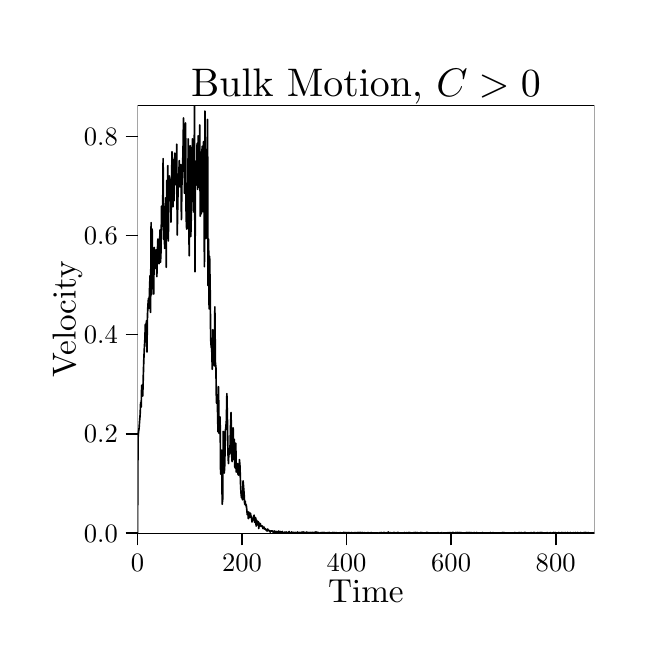
\begin{tikzpicture}[x=1pt,y=1pt]
\definecolor[named]{fillColor}{rgb}{1.00,1.00,1.00}
\path[use as bounding box,fill=fillColor,fill opacity=0.00] (0,0) rectangle (216.81,216.81);
\begin{scope}
\path[clip] (  0.00,  0.00) rectangle (216.81,216.81);
\definecolor[named]{drawColor}{rgb}{1.00,1.00,1.00}
\definecolor[named]{fillColor}{rgb}{1.00,1.00,1.00}

\path[draw=drawColor,line width= 0.6pt,line join=round,line cap=round,fill=fillColor] ( -0.00,  0.00) rectangle (216.81,216.81);
\end{scope}
\begin{scope}
\path[clip] ( 39.69, 34.03) rectangle (204.76,188.82);
\definecolor[named]{fillColor}{rgb}{1.00,1.00,1.00}

\path[fill=fillColor] ( 39.69, 34.03) rectangle (204.76,188.82);
\definecolor[named]{drawColor}{rgb}{0.00,0.00,0.00}

\path[draw=drawColor,line width= 0.6pt,line join=round] ( 39.69, 34.21) --
	( 39.88, 68.43) --
	( 40.06, 70.76) --
	( 40.25, 72.02) --
	( 40.44, 74.70) --
	( 40.63, 76.85) --
	( 40.82, 81.33) --
	( 41.01, 79.72) --
	( 41.20, 87.60) --
	( 41.39, 87.60) --
	( 41.58, 83.66) --
	( 41.76, 90.29) --
	( 41.95, 96.38) --
	( 42.14,100.68) --
	( 42.33,103.91) --
	( 42.52,109.64) --
	( 42.71,105.88) --
	( 42.90,110.89) --
	( 43.09, 99.61) --
	( 43.28,112.68) --
	( 43.46,116.63) --
	( 43.65,118.95) --
	( 43.84,115.37) --
	( 44.03,122.18) --
	( 44.22,127.20) --
	( 44.41,113.94) --
	( 44.60,146.37) --
	( 44.79,120.39) --
	( 44.98,144.04) --
	( 45.16,128.27) --
	( 45.35,136.69) --
	( 45.54,120.57) --
	( 45.73,137.41) --
	( 45.92,129.70) --
	( 46.11,136.51) --
	( 46.30,135.44) --
	( 46.49,136.51) --
	( 46.68,126.84) --
	( 46.86,135.62) --
	( 47.05,140.45) --
	( 47.24,136.33) --
	( 47.43,131.50) --
	( 47.62,135.97) --
	( 47.81,143.68) --
	( 48.00,132.03) --
	( 48.19,136.15) --
	( 48.37,152.28) --
	( 48.56,145.83) --
	( 48.75,145.11) --
	( 48.94,169.48) --
	( 49.13,140.27) --
	( 49.32,143.86) --
	( 49.51,137.05) --
	( 49.70,149.05) --
	( 49.89,155.32) --
	( 50.07,130.24) --
	( 50.26,161.59) --
	( 50.45,145.83) --
	( 50.64,166.97) --
	( 50.83,139.74) --
	( 51.02,162.85) --
	( 51.21,163.21) --
	( 51.40,156.22) --
	( 51.59,161.95) --
	( 51.77,146.54) --
	( 51.96,156.94) --
	( 52.15,171.98) --
	( 52.34,164.10) --
	( 52.53,152.10) --
	( 52.72,169.12) --
	( 52.91,154.25) --
	( 53.10,171.45) --
	( 53.29,169.30) --
	( 53.47,171.27) --
	( 53.66,159.98) --
	( 53.85,174.67) --
	( 54.04,141.89) --
	( 54.23,152.64) --
	( 54.42,161.95) --
	( 54.61,163.92) --
	( 54.80,168.76) --
	( 54.99,159.26) --
	( 55.17,162.13) --
	( 55.36,167.33) --
	( 55.55,147.44) --
	( 55.74,160.34) --
	( 55.93,165.00) --
	( 56.12,171.81) --
	( 56.31,184.17) --
	( 56.50,177.18) --
	( 56.69,156.94) --
	( 56.87,161.41) --
	( 57.06,182.38) --
	( 57.25,148.51) --
	( 57.44,144.04) --
	( 57.63,145.11) --
	( 57.82,148.69) --
	( 58.01,176.64) --
	( 58.20,145.83) --
	( 58.39,134.36) --
	( 58.57,170.91) --
	( 58.76,174.13) --
	( 58.95,141.35) --
	( 59.14,149.77) --
	( 59.33,151.20) --
	( 59.52,176.64) --
	( 59.71,164.46) --
	( 59.90,170.55) --
	( 60.09,150.13) --
	( 60.27,188.82) --
	( 60.46,128.63) --
	( 60.65,167.51) --
	( 60.84,168.58) --
	( 61.03,159.98) --
	( 61.22,175.03) --
	( 61.41,158.37) --
	( 61.60,177.72) --
	( 61.79,166.61) --
	( 61.97,159.09) --
	( 62.16,181.66) --
	( 62.35,148.69) --
	( 62.54,149.95) --
	( 62.73,149.59) --
	( 62.92,171.98) --
	( 63.11,173.96) --
	( 63.30,150.31) --
	( 63.49,175.57) --
	( 63.67,169.30) --
	( 63.86,130.42) --
	( 64.05,186.68) --
	( 64.24,166.25) --
	( 64.43,140.63) --
	( 64.62,161.95) --
	( 64.81,159.09) --
	( 65.00,183.63) --
	( 65.18,123.61) --
	( 65.37,140.45) --
	( 65.56,115.19) --
	( 65.75,134.18) --
	( 65.94,122.36) --
	( 66.13,104.26) --
	( 66.32,101.40) --
	( 66.51,100.86) --
	( 66.70, 93.34) --
	( 66.88,107.67) --
	( 67.07,105.52) --
	( 67.26,101.58) --
	( 67.45, 94.59) --
	( 67.64,115.91) --
	( 67.83, 95.84) --
	( 68.02, 94.05) --
	( 68.21, 81.15) --
	( 68.40, 84.20) --
	( 68.58, 79.90) --
	( 68.77, 70.76) --
	( 68.96, 87.06) --
	( 69.15, 70.22) --
	( 69.34, 74.52) --
	( 69.53, 76.14) --
	( 69.72, 55.53) --
	( 69.91, 56.25) --
	( 70.10, 64.13) --
	( 70.28, 44.60) --
	( 70.47, 46.40) --
	( 70.66, 70.94) --
	( 70.85, 61.45) --
	( 71.04, 55.89) --
	( 71.23, 59.12) --
	( 71.42, 71.12) --
	( 71.61, 72.37) --
	( 71.80, 74.88) --
	( 71.98, 84.56) --
	( 72.17, 75.60) --
	( 72.36, 63.42) --
	( 72.55, 59.30) --
	( 72.74, 64.67) --
	( 72.93, 62.70) --
	( 73.12, 65.21) --
	( 73.31, 72.91) --
	( 73.50, 77.75) --
	( 73.68, 62.88) --
	( 73.87, 60.01) --
	( 74.06, 68.79) --
	( 74.25, 72.19) --
	( 74.44, 60.73) --
	( 74.63, 68.07) --
	( 74.82, 58.22) --
	( 75.01, 57.68) --
	( 75.20, 66.64) --
	( 75.38, 56.25) --
	( 75.57, 56.43) --
	( 75.76, 59.30) --
	( 75.95, 55.71) --
	( 76.14, 55.17) --
	( 76.33, 55.17) --
	( 76.52, 60.73) --
	( 76.71, 58.40) --
	( 76.90, 52.49) --
	( 77.08, 48.73) --
	( 77.27, 46.93) --
	( 77.46, 48.37) --
	( 77.65, 46.22) --
	( 77.84, 53.03) --
	( 78.03, 50.70) --
	( 78.22, 48.19) --
	( 78.41, 44.60) --
	( 78.60, 45.68) --
	( 78.78, 44.07) --
	( 78.97, 44.43) --
	( 79.16, 42.81) --
	( 79.35, 40.84) --
	( 79.54, 41.92) --
	( 79.73, 39.41) --
	( 79.92, 41.74) --
	( 80.11, 40.66) --
	( 80.30, 39.77) --
	( 80.48, 41.38) --
	( 80.67, 40.31) --
	( 80.86, 40.31) --
	( 81.05, 38.16) --
	( 81.24, 39.59) --
	( 81.43, 39.41) --
	( 81.62, 38.87) --
	( 81.81, 40.66) --
	( 81.99, 38.16) --
	( 82.18, 37.98) --
	( 82.37, 39.77) --
	( 82.56, 36.72) --
	( 82.75, 38.87) --
	( 82.94, 37.26) --
	( 83.13, 37.80) --
	( 83.32, 38.33) --
	( 83.51, 35.83) --
	( 83.69, 37.80) --
	( 83.88, 36.90) --
	( 84.07, 37.62) --
	( 84.26, 36.72) --
	( 84.45, 36.54) --
	( 84.64, 36.72) --
	( 84.83, 36.72) --
	( 85.02, 35.83) --
	( 85.21, 36.18) --
	( 85.39, 36.36) --
	( 85.58, 35.65) --
	( 85.77, 35.83) --
	( 85.96, 35.65) --
	( 86.15, 35.29) --
	( 86.34, 35.11) --
	( 86.53, 34.93) --
	( 86.72, 35.65) --
	( 86.91, 35.29) --
	( 87.09, 35.11) --
	( 87.28, 35.11) --
	( 87.47, 34.75) --
	( 87.66, 34.57) --
	( 87.85, 34.93) --
	( 88.04, 34.93) --
	( 88.23, 34.93) --
	( 88.42, 34.93) --
	( 88.61, 34.75) --
	( 88.79, 34.39) --
	( 88.98, 34.57) --
	( 89.17, 34.93) --
	( 89.36, 34.39) --
	( 89.55, 34.75) --
	( 89.74, 34.21) --
	( 89.93, 34.75) --
	( 90.12, 34.21) --
	( 90.31, 34.03) --
	( 90.49, 34.39) --
	( 90.68, 34.93) --
	( 90.87, 34.39) --
	( 91.06, 34.39) --
	( 91.25, 34.75) --
	( 91.44, 34.39) --
	( 91.63, 34.57) --
	( 91.82, 34.21) --
	( 92.01, 34.75) --
	( 92.19, 34.39) --
	( 92.38, 34.21) --
	( 92.57, 34.39) --
	( 92.76, 34.21) --
	( 92.95, 34.57) --
	( 93.14, 34.21) --
	( 93.33, 34.39) --
	( 93.52, 34.57) --
	( 93.71, 34.21) --
	( 93.89, 34.21) --
	( 94.08, 34.39) --
	( 94.27, 34.21) --
	( 94.46, 34.75) --
	( 94.65, 34.03) --
	( 94.84, 34.21) --
	( 95.03, 34.39) --
	( 95.22, 34.21) --
	( 95.41, 34.57) --
	( 95.59, 34.39) --
	( 95.78, 34.21) --
	( 95.97, 34.39) --
	( 96.16, 34.39) --
	( 96.35, 34.21) --
	( 96.54, 34.39) --
	( 96.73, 34.39) --
	( 96.92, 34.21) --
	( 97.11, 34.21) --
	( 97.29, 34.21) --
	( 97.48, 34.57) --
	( 97.67, 34.21) --
	( 97.86, 34.21) --
	( 98.05, 34.39) --
	( 98.24, 34.39) --
	( 98.43, 34.21) --
	( 98.62, 34.39) --
	( 98.81, 34.03) --
	( 98.99, 34.39) --
	( 99.18, 34.57) --
	( 99.37, 34.21) --
	( 99.56, 34.21) --
	( 99.75, 34.57) --
	( 99.94, 34.03) --
	(100.13, 34.39) --
	(100.32, 34.03) --
	(100.50, 34.39) --
	(100.69, 34.03) --
	(100.88, 34.57) --
	(101.07, 34.03) --
	(101.26, 34.21) --
	(101.45, 34.39) --
	(101.64, 34.03) --
	(101.83, 34.39) --
	(102.02, 34.21) --
	(102.20, 34.39) --
	(102.39, 34.39) --
	(102.58, 34.21) --
	(102.77, 34.39) --
	(102.96, 34.39) --
	(103.15, 34.21) --
	(103.34, 34.39) --
	(103.53, 34.03) --
	(103.72, 34.21) --
	(103.90, 34.57) --
	(104.09, 34.21) --
	(104.28, 34.03) --
	(104.47, 34.57) --
	(104.66, 34.21) --
	(104.85, 34.03) --
	(105.04, 34.39) --
	(105.23, 34.21) --
	(105.42, 34.21) --
	(105.60, 34.03) --
	(105.79, 34.21) --
	(105.98, 34.39) --
	(106.17, 34.21) --
	(106.36, 34.39) --
	(106.55, 34.03) --
	(106.74, 34.21) --
	(106.93, 34.39) --
	(107.12, 34.03) --
	(107.30, 34.39) --
	(107.49, 34.21) --
	(107.68, 34.21) --
	(107.87, 34.21) --
	(108.06, 34.21) --
	(108.25, 34.39) --
	(108.44, 34.21) --
	(108.63, 34.03) --
	(108.82, 34.39) --
	(109.00, 34.39) --
	(109.19, 34.21) --
	(109.38, 34.21) --
	(109.57, 34.21) --
	(109.76, 34.21) --
	(109.95, 34.21) --
	(110.14, 34.39) --
	(110.33, 34.03) --
	(110.52, 34.21) --
	(110.70, 34.39) --
	(110.89, 34.03) --
	(111.08, 34.21) --
	(111.27, 34.21) --
	(111.46, 34.39) --
	(111.65, 34.21) --
	(111.84, 34.21) --
	(112.03, 34.21) --
	(112.22, 34.21) --
	(112.40, 34.21) --
	(112.59, 34.21) --
	(112.78, 34.21) --
	(112.97, 34.39) --
	(113.16, 34.21) --
	(113.35, 34.21) --
	(113.54, 34.21) --
	(113.73, 34.21) --
	(113.92, 34.21) --
	(114.10, 34.39) --
	(114.29, 34.39) --
	(114.48, 34.03) --
	(114.67, 34.39) --
	(114.86, 34.03) --
	(115.05, 34.21) --
	(115.24, 34.39) --
	(115.43, 34.21) --
	(115.62, 34.03) --
	(115.80, 34.39) --
	(115.99, 34.03) --
	(116.18, 34.21) --
	(116.37, 34.39) --
	(116.56, 34.21) --
	(116.75, 34.21) --
	(116.94, 34.03) --
	(117.13, 34.39) --
	(117.31, 34.21) --
	(117.50, 34.21) --
	(117.69, 34.03) --
	(117.88, 34.21) --
	(118.07, 34.39) --
	(118.26, 34.21) --
	(118.45, 34.21) --
	(118.64, 34.39) --
	(118.83, 34.21) --
	(119.01, 34.03) --
	(119.20, 34.39) --
	(119.39, 34.03) --
	(119.58, 34.39) --
	(119.77, 34.03) --
	(119.96, 34.39) --
	(120.15, 34.03) --
	(120.34, 34.39) --
	(120.53, 34.21) --
	(120.71, 34.03) --
	(120.90, 34.39) --
	(121.09, 34.21) --
	(121.28, 34.21) --
	(121.47, 34.21) --
	(121.66, 34.39) --
	(121.85, 34.21) --
	(122.04, 34.03) --
	(122.23, 34.21) --
	(122.41, 34.21) --
	(122.60, 34.21) --
	(122.79, 34.21) --
	(122.98, 34.39) --
	(123.17, 34.03) --
	(123.36, 34.21) --
	(123.55, 34.21) --
	(123.74, 34.21) --
	(123.93, 34.03) --
	(124.11, 34.39) --
	(124.30, 34.21) --
	(124.49, 34.21) --
	(124.68, 34.21) --
	(124.87, 34.21) --
	(125.06, 34.21) --
	(125.25, 34.21) --
	(125.44, 34.21) --
	(125.63, 34.21) --
	(125.81, 34.21) --
	(126.00, 34.21) --
	(126.19, 34.21) --
	(126.38, 34.21) --
	(126.57, 34.21) --
	(126.76, 34.21) --
	(126.95, 34.03) --
	(127.14, 34.21) --
	(127.33, 34.39) --
	(127.51, 34.21) --
	(127.70, 34.21) --
	(127.89, 34.39) --
	(128.08, 34.03) --
	(128.27, 34.21) --
	(128.46, 34.21) --
	(128.65, 34.39) --
	(128.84, 34.03) --
	(129.03, 34.39) --
	(129.21, 34.21) --
	(129.40, 34.21) --
	(129.59, 34.21) --
	(129.78, 34.21) --
	(129.97, 34.39) --
	(130.16, 34.03) --
	(130.35, 34.57) --
	(130.54, 34.03) --
	(130.73, 34.21) --
	(130.91, 34.21) --
	(131.10, 34.39) --
	(131.29, 34.21) --
	(131.48, 34.21) --
	(131.67, 34.21) --
	(131.86, 34.03) --
	(132.05, 34.21) --
	(132.24, 34.39) --
	(132.43, 34.03) --
	(132.61, 34.39) --
	(132.80, 34.21) --
	(132.99, 34.21) --
	(133.18, 34.21) --
	(133.37, 34.21) --
	(133.56, 34.39) --
	(133.75, 34.03) --
	(133.94, 34.39) --
	(134.13, 34.03) --
	(134.31, 34.21) --
	(134.50, 34.21) --
	(134.69, 34.21) --
	(134.88, 34.21) --
	(135.07, 34.21) --
	(135.26, 34.21) --
	(135.45, 34.21) --
	(135.64, 34.21) --
	(135.82, 34.21) --
	(136.01, 34.21) --
	(136.20, 34.39) --
	(136.39, 34.03) --
	(136.58, 34.21) --
	(136.77, 34.21) --
	(136.96, 34.39) --
	(137.15, 34.21) --
	(137.34, 34.21) --
	(137.52, 34.03) --
	(137.71, 34.39) --
	(137.90, 34.03) --
	(138.09, 34.39) --
	(138.28, 34.21) --
	(138.47, 34.21) --
	(138.66, 34.21) --
	(138.85, 34.21) --
	(139.04, 34.21) --
	(139.22, 34.21) --
	(139.41, 34.21) --
	(139.60, 34.39) --
	(139.79, 34.03) --
	(139.98, 34.21) --
	(140.17, 34.39) --
	(140.36, 34.03) --
	(140.55, 34.21) --
	(140.74, 34.39) --
	(140.92, 34.03) --
	(141.11, 34.21) --
	(141.30, 34.21) --
	(141.49, 34.21) --
	(141.68, 34.21) --
	(141.87, 34.03) --
	(142.06, 34.39) --
	(142.25, 34.21) --
	(142.44, 34.39) --
	(142.62, 34.03) --
	(142.81, 34.21) --
	(143.00, 34.21) --
	(143.19, 34.21) --
	(143.38, 34.21) --
	(143.57, 34.21) --
	(143.76, 34.21) --
	(143.95, 34.21) --
	(144.14, 34.39) --
	(144.32, 34.03) --
	(144.51, 34.39) --
	(144.70, 34.21) --
	(144.89, 34.03) --
	(145.08, 34.21) --
	(145.27, 34.21) --
	(145.46, 34.21) --
	(145.65, 34.21) --
	(145.84, 34.21) --
	(146.02, 34.21) --
	(146.21, 34.21) --
	(146.40, 34.21) --
	(146.59, 34.21) --
	(146.78, 34.21) --
	(146.97, 34.21) --
	(147.16, 34.21) --
	(147.35, 34.21) --
	(147.54, 34.21) --
	(147.72, 34.21) --
	(147.91, 34.21) --
	(148.10, 34.21) --
	(148.29, 34.39) --
	(148.48, 34.21) --
	(148.67, 34.21) --
	(148.86, 34.03) --
	(149.05, 34.21) --
	(149.24, 34.21) --
	(149.42, 34.21) --
	(149.61, 34.39) --
	(149.80, 34.21) --
	(149.99, 34.03) --
	(150.18, 34.21) --
	(150.37, 34.21) --
	(150.56, 34.21) --
	(150.75, 34.21) --
	(150.94, 34.21) --
	(151.12, 34.21) --
	(151.31, 34.21) --
	(151.50, 34.21) --
	(151.69, 34.21) --
	(151.88, 34.39) --
	(152.07, 34.21) --
	(152.26, 34.21) --
	(152.45, 34.03) --
	(152.63, 34.39) --
	(152.82, 34.21) --
	(153.01, 34.21) --
	(153.20, 34.03) --
	(153.39, 34.39) --
	(153.58, 34.03) --
	(153.77, 34.39) --
	(153.96, 34.21) --
	(154.15, 34.21) --
	(154.33, 34.03) --
	(154.52, 34.39) --
	(154.71, 34.03) --
	(154.90, 34.21) --
	(155.09, 34.39) --
	(155.28, 34.03) --
	(155.47, 34.39) --
	(155.66, 34.21) --
	(155.85, 34.21) --
	(156.03, 34.39) --
	(156.22, 34.03) --
	(156.41, 34.03) --
	(156.60, 34.39) --
	(156.79, 34.21) --
	(156.98, 34.21) --
	(157.17, 34.21) --
	(157.36, 34.21) --
	(157.55, 34.21) --
	(157.73, 34.21) --
	(157.92, 34.21) --
	(158.11, 34.21) --
	(158.30, 34.03) --
	(158.49, 34.39) --
	(158.68, 34.21) --
	(158.87, 34.03) --
	(159.06, 34.39) --
	(159.25, 34.21) --
	(159.43, 34.39) --
	(159.62, 34.03) --
	(159.81, 34.39) --
	(160.00, 34.03) --
	(160.19, 34.21) --
	(160.38, 34.39) --
	(160.57, 34.21) --
	(160.76, 34.21) --
	(160.95, 34.21) --
	(161.13, 34.03) --
	(161.32, 34.39) --
	(161.51, 34.21) --
	(161.70, 34.21) --
	(161.89, 34.21) --
	(162.08, 34.03) --
	(162.27, 34.39) --
	(162.46, 34.21) --
	(162.65, 34.21) --
	(162.83, 34.21) --
	(163.02, 34.21) --
	(163.21, 34.21) --
	(163.40, 34.21) --
	(163.59, 34.21) --
	(163.78, 34.21) --
	(163.97, 34.21) --
	(164.16, 34.03) --
	(164.35, 34.39) --
	(164.53, 34.21) --
	(164.72, 34.21) --
	(164.91, 34.21) --
	(165.10, 34.21) --
	(165.29, 34.21) --
	(165.48, 34.21) --
	(165.67, 34.21) --
	(165.86, 34.21) --
	(166.05, 34.21) --
	(166.23, 34.21) --
	(166.42, 34.21) --
	(166.61, 34.21) --
	(166.80, 34.21) --
	(166.99, 34.03) --
	(167.18, 34.39) --
	(167.37, 34.03) --
	(167.56, 34.21) --
	(167.75, 34.21) --
	(167.93, 34.21) --
	(168.12, 34.39) --
	(168.31, 34.21) --
	(168.50, 34.21) --
	(168.69, 34.21) --
	(168.88, 34.21) --
	(169.07, 34.21) --
	(169.26, 34.21) --
	(169.45, 34.21) --
	(169.63, 34.21) --
	(169.82, 34.21) --
	(170.01, 34.21) --
	(170.20, 34.21) --
	(170.39, 34.21) --
	(170.58, 34.21) --
	(170.77, 34.21) --
	(170.96, 34.21) --
	(171.14, 34.21) --
	(171.33, 34.21) --
	(171.52, 34.39) --
	(171.71, 34.03) --
	(171.90, 34.21) --
	(172.09, 34.39) --
	(172.28, 34.03) --
	(172.47, 34.21) --
	(172.66, 34.21) --
	(172.84, 34.21) --
	(173.03, 34.21) --
	(173.22, 34.21) --
	(173.41, 34.21) --
	(173.60, 34.21) --
	(173.79, 34.21) --
	(173.98, 34.21) --
	(174.17, 34.21) --
	(174.36, 34.21) --
	(174.54, 34.21) --
	(174.73, 34.21) --
	(174.92, 34.21) --
	(175.11, 34.21) --
	(175.30, 34.21) --
	(175.49, 34.21) --
	(175.68, 34.21) --
	(175.87, 34.21) --
	(176.06, 34.39) --
	(176.24, 34.03) --
	(176.43, 34.21) --
	(176.62, 34.21) --
	(176.81, 34.21) --
	(177.00, 34.21) --
	(177.19, 34.21) --
	(177.38, 34.21) --
	(177.57, 34.39) --
	(177.76, 34.03) --
	(177.94, 34.21) --
	(178.13, 34.21) --
	(178.32, 34.39) --
	(178.51, 34.03) --
	(178.70, 34.21) --
	(178.89, 34.21) --
	(179.08, 34.21) --
	(179.27, 34.21) --
	(179.46, 34.39) --
	(179.64, 34.03) --
	(179.83, 34.39) --
	(180.02, 34.03) --
	(180.21, 34.21) --
	(180.40, 34.21) --
	(180.59, 34.21) --
	(180.78, 34.21) --
	(180.97, 34.21) --
	(181.16, 34.21) --
	(181.34, 34.21) --
	(181.53, 34.21) --
	(181.72, 34.21) --
	(181.91, 34.39) --
	(182.10, 34.21) --
	(182.29, 34.21) --
	(182.48, 34.21) --
	(182.67, 34.03) --
	(182.86, 34.39) --
	(183.04, 34.03) --
	(183.23, 34.39) --
	(183.42, 34.21) --
	(183.61, 34.03) --
	(183.80, 34.21) --
	(183.99, 34.21) --
	(184.18, 34.21) --
	(184.37, 34.39) --
	(184.56, 34.03) --
	(184.74, 34.21) --
	(184.93, 34.21) --
	(185.12, 34.39) --
	(185.31, 34.03) --
	(185.50, 34.39) --
	(185.69, 34.03) --
	(185.88, 34.39) --
	(186.07, 34.03) --
	(186.26, 34.21) --
	(186.44, 34.21) --
	(186.63, 34.21) --
	(186.82, 34.21) --
	(187.01, 34.21) --
	(187.20, 34.21) --
	(187.39, 34.21) --
	(187.58, 34.21) --
	(187.77, 34.39) --
	(187.95, 34.21) --
	(188.14, 34.03) --
	(188.33, 34.21) --
	(188.52, 34.21) --
	(188.71, 34.21) --
	(188.90, 34.39) --
	(189.09, 34.21) --
	(189.28, 34.03) --
	(189.47, 34.21) --
	(189.65, 34.21) --
	(189.84, 34.21) --
	(190.03, 34.39) --
	(190.22, 34.03) --
	(190.41, 34.21) --
	(190.60, 34.39) --
	(190.79, 34.03) --
	(190.98, 34.21) --
	(191.17, 34.21) --
	(191.35, 34.21) --
	(191.54, 34.21) --
	(191.73, 34.21) --
	(191.92, 34.39) --
	(192.11, 34.03) --
	(192.30, 34.21) --
	(192.49, 34.21) --
	(192.68, 34.21) --
	(192.87, 34.39) --
	(193.05, 34.03) --
	(193.24, 34.21) --
	(193.43, 34.39) --
	(193.62, 34.21) --
	(193.81, 34.21) --
	(194.00, 34.03) --
	(194.19, 34.39) --
	(194.38, 34.21) --
	(194.57, 34.21) --
	(194.75, 34.21) --
	(194.94, 34.03) --
	(195.13, 34.39) --
	(195.32, 34.21) --
	(195.51, 34.21) --
	(195.70, 34.21) --
	(195.89, 34.03) --
	(196.08, 34.39) --
	(196.27, 34.21) --
	(196.45, 34.03) --
	(196.64, 34.21) --
	(196.83, 34.21) --
	(197.02, 34.21) --
	(197.21, 34.39) --
	(197.40, 34.21) --
	(197.59, 34.21) --
	(197.78, 34.03) --
	(197.97, 34.39) --
	(198.15, 34.21) --
	(198.34, 34.21) --
	(198.53, 34.03) --
	(198.72, 34.39) --
	(198.91, 34.21) --
	(199.10, 34.21) --
	(199.29, 34.21) --
	(199.48, 34.21) --
	(199.67, 34.03) --
	(199.85, 34.39) --
	(200.04, 34.21) --
	(200.23, 34.21) --
	(200.42, 34.21) --
	(200.61, 34.21) --
	(200.80, 34.03) --
	(200.99, 34.39) --
	(201.18, 34.03) --
	(201.37, 34.39) --
	(201.55, 34.03) --
	(201.74, 34.39) --
	(201.93, 34.21) --
	(202.12, 34.21) --
	(202.31, 34.03) --
	(202.50, 34.39) --
	(202.69, 34.21) --
	(202.88, 34.21) --
	(203.07, 34.21) --
	(203.25, 34.21) --
	(203.44, 34.21) --
	(203.63, 34.21) --
	(203.82, 34.21) --
	(204.01, 34.21) --
	(204.20, 34.21) --
	(204.39, 34.21) --
	(204.58, 34.21) --
	(204.76, 34.39);

\path[draw=drawColor,line width= 0.6pt,line join=round,line cap=round] ( 39.69, 34.03) rectangle (204.76,188.82);
\end{scope}
\begin{scope}
\path[clip] (  0.00,  0.00) rectangle (216.81,216.81);
\definecolor[named]{drawColor}{rgb}{0.00,0.00,0.00}

\node[text=drawColor,anchor=base east,inner sep=0pt, outer sep=0pt, scale=  0.96] at ( 32.57, 30.91) {0.0};

\node[text=drawColor,anchor=base east,inner sep=0pt, outer sep=0pt, scale=  0.96] at ( 32.57, 66.74) {0.2};

\node[text=drawColor,anchor=base east,inner sep=0pt, outer sep=0pt, scale=  0.96] at ( 32.57,102.57) {0.4};

\node[text=drawColor,anchor=base east,inner sep=0pt, outer sep=0pt, scale=  0.96] at ( 32.57,138.40) {0.6};

\node[text=drawColor,anchor=base east,inner sep=0pt, outer sep=0pt, scale=  0.96] at ( 32.57,174.23) {0.8};
\end{scope}
\begin{scope}
\path[clip] (  0.00,  0.00) rectangle (216.81,216.81);
\definecolor[named]{drawColor}{rgb}{0.00,0.00,0.00}

\path[draw=drawColor,line width= 0.6pt,line join=round] ( 35.42, 34.21) --
	( 39.69, 34.21);

\path[draw=drawColor,line width= 0.6pt,line join=round] ( 35.42, 70.04) --
	( 39.69, 70.04);

\path[draw=drawColor,line width= 0.6pt,line join=round] ( 35.42,105.88) --
	( 39.69,105.88);

\path[draw=drawColor,line width= 0.6pt,line join=round] ( 35.42,141.71) --
	( 39.69,141.71);

\path[draw=drawColor,line width= 0.6pt,line join=round] ( 35.42,177.54) --
	( 39.69,177.54);
\end{scope}
\begin{scope}
\path[clip] (  0.00,  0.00) rectangle (216.81,216.81);
\definecolor[named]{drawColor}{rgb}{0.00,0.00,0.00}

\path[draw=drawColor,line width= 0.6pt,line join=round] ( 39.69, 29.77) --
	( 39.69, 34.03);

\path[draw=drawColor,line width= 0.6pt,line join=round] ( 77.46, 29.77) --
	( 77.46, 34.03);

\path[draw=drawColor,line width= 0.6pt,line join=round] (115.24, 29.77) --
	(115.24, 34.03);

\path[draw=drawColor,line width= 0.6pt,line join=round] (153.01, 29.77) --
	(153.01, 34.03);

\path[draw=drawColor,line width= 0.6pt,line join=round] (190.79, 29.77) --
	(190.79, 34.03);
\end{scope}
\begin{scope}
\path[clip] (  0.00,  0.00) rectangle (216.81,216.81);
\definecolor[named]{drawColor}{rgb}{0.00,0.00,0.00}

\node[text=drawColor,anchor=base,inner sep=0pt, outer sep=0pt, scale=  0.96] at ( 39.69, 20.31) {0};

\node[text=drawColor,anchor=base,inner sep=0pt, outer sep=0pt, scale=  0.96] at ( 77.46, 20.31) {200};

\node[text=drawColor,anchor=base,inner sep=0pt, outer sep=0pt, scale=  0.96] at (115.24, 20.31) {400};

\node[text=drawColor,anchor=base,inner sep=0pt, outer sep=0pt, scale=  0.96] at (153.01, 20.31) {600};

\node[text=drawColor,anchor=base,inner sep=0pt, outer sep=0pt, scale=  0.96] at (190.79, 20.31) {800};
\end{scope}
\begin{scope}
\path[clip] (  0.00,  0.00) rectangle (216.81,216.81);
\definecolor[named]{drawColor}{rgb}{0.00,0.00,0.00}

\node[text=drawColor,anchor=base,inner sep=0pt, outer sep=0pt, scale=  1.20] at (122.23,  9.03) {Time};
\end{scope}
\begin{scope}
\path[clip] (  0.00,  0.00) rectangle (216.81,216.81);
\definecolor[named]{drawColor}{rgb}{0.00,0.00,0.00}

\node[text=drawColor,rotate= 90.00,anchor=base,inner sep=0pt, outer sep=0pt, scale=  1.20] at ( 17.30,111.43) {Velocity};
\end{scope}
\begin{scope}
\path[clip] (  0.00,  0.00) rectangle (216.81,216.81);
\definecolor[named]{drawColor}{rgb}{0.00,0.00,0.00}

\node[text=drawColor,anchor=base,inner sep=0pt, outer sep=0pt, scale=  1.44] at (122.23,191.84) {Bulk Motion, $C > 0$};
\end{scope}
\end{tikzpicture}

		\caption{Simulation with the positive mutation probability rate.}
	\end{subfigure}
	\begin{subfigure}[h]{0.5 \textwidth}
		% Created by tikzDevice version 0.7.0 on 2015-04-28 18:09:54
% !TEX encoding = UTF-8 Unicode
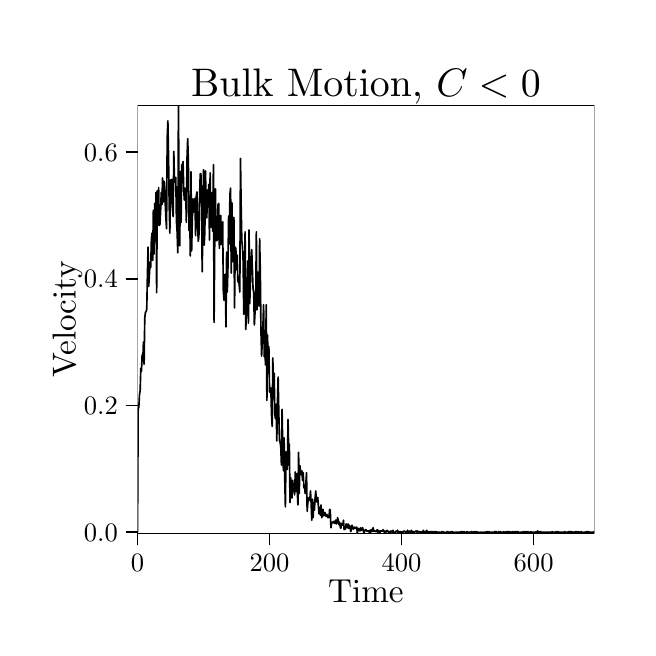
\begin{tikzpicture}[x=1pt,y=1pt]
\definecolor[named]{fillColor}{rgb}{1.00,1.00,1.00}
\path[use as bounding box,fill=fillColor,fill opacity=0.00] (0,0) rectangle (216.81,216.81);
\begin{scope}
\path[clip] (  0.00,  0.00) rectangle (216.81,216.81);
\definecolor[named]{drawColor}{rgb}{1.00,1.00,1.00}
\definecolor[named]{fillColor}{rgb}{1.00,1.00,1.00}

\path[draw=drawColor,line width= 0.6pt,line join=round,line cap=round,fill=fillColor] ( -0.00,  0.00) rectangle (216.81,216.81);
\end{scope}
\begin{scope}
\path[clip] ( 39.69, 34.03) rectangle (204.76,188.82);
\definecolor[named]{fillColor}{rgb}{1.00,1.00,1.00}

\path[fill=fillColor] ( 39.69, 34.03) rectangle (204.76,188.82);
\definecolor[named]{drawColor}{rgb}{0.00,0.00,0.00}

\path[draw=drawColor,line width= 0.6pt,line join=round] ( 39.69, 34.49) --
	( 39.93, 79.14) --
	( 40.16, 79.60) --
	( 40.40, 84.18) --
	( 40.64, 85.56) --
	( 40.88, 93.80) --
	( 41.12, 92.65) --
	( 41.36, 98.61) --
	( 41.59, 96.32) --
	( 41.83,103.19) --
	( 42.07, 95.17) --
	( 42.31,111.89) --
	( 42.55,113.95) --
	( 42.79,114.18) --
	( 43.03,115.09) --
	( 43.26,127.23) --
	( 43.50,137.53) --
	( 43.74,123.34) --
	( 43.98,127.46) --
	( 44.22,132.04) --
	( 44.46,130.21) --
	( 44.70,140.28) --
	( 44.93,142.57) --
	( 45.17,132.72) --
	( 45.41,150.81) --
	( 45.65,135.01) --
	( 45.89,153.33) --
	( 46.13,140.28) --
	( 46.37,157.23) --
	( 46.60,121.05) --
	( 46.84,157.91) --
	( 47.08,145.55) --
	( 47.32,159.06) --
	( 47.56,145.32) --
	( 47.80,145.78) --
	( 48.04,150.59) --
	( 48.27,157.23) --
	( 48.51,152.88) --
	( 48.75,162.49) --
	( 48.99,153.79) --
	( 49.23,161.35) --
	( 49.47,160.66) --
	( 49.71,153.10) --
	( 49.94,148.07) --
	( 50.18,144.17) --
	( 50.42,176.92) --
	( 50.66,183.10) --
	( 50.90,170.28) --
	( 51.14,152.65) --
	( 51.38,142.57) --
	( 51.61,161.81) --
	( 51.85,153.33) --
	( 52.09,162.03) --
	( 52.33,150.81) --
	( 52.57,148.52) --
	( 52.81,172.11) --
	( 53.05,160.89) --
	( 53.28,162.72) --
	( 53.52,162.72) --
	( 53.76,146.69) --
	( 54.00,143.03) --
	( 54.24,135.47) --
	( 54.48,188.82) --
	( 54.72,152.42) --
	( 54.95,137.99) --
	( 55.19,164.78) --
	( 55.43,146.46) --
	( 55.67,167.30) --
	( 55.91,166.61) --
	( 56.15,168.45) --
	( 56.39,158.14) --
	( 56.62,154.48) --
	( 56.86,158.83) --
	( 57.10,157.68) --
	( 57.34,146.46) --
	( 57.58,169.59) --
	( 57.82,176.69) --
	( 58.06,168.90) --
	( 58.29,143.49) --
	( 58.53,151.73) --
	( 58.77,134.33) --
	( 59.01,164.78) --
	( 59.25,136.16) --
	( 59.49,147.38) --
	( 59.72,154.94) --
	( 59.96,150.13) --
	( 60.20,153.33) --
	( 60.44,155.16) --
	( 60.68,141.66) --
	( 60.92,155.85) --
	( 61.16,157.45) --
	( 61.39,147.15) --
	( 61.63,139.59) --
	( 61.87,141.43) --
	( 62.11,155.16) --
	( 62.35,163.87) --
	( 62.59,164.10) --
	( 62.83,154.48) --
	( 63.06,128.60) --
	( 63.30,145.09) --
	( 63.54,165.47) --
	( 63.78,138.22) --
	( 64.02,143.03) --
	( 64.26,165.01) --
	( 64.50,149.90) --
	( 64.73,148.07) --
	( 64.97,158.14) --
	( 65.21,155.16) --
	( 65.45,160.20) --
	( 65.69,140.05) --
	( 65.93,164.32) --
	( 66.17,147.84) --
	( 66.40,144.63) --
	( 66.64,157.23) --
	( 66.88,143.26) --
	( 67.12,167.30) --
	( 67.36,110.28) --
	( 67.60,141.43) --
	( 67.84,158.60) --
	( 68.07,140.51) --
	( 68.31,139.82) --
	( 68.55,140.28) --
	( 68.79,152.88) --
	( 69.03,153.33) --
	( 69.27,137.08) --
	( 69.51,146.92) --
	( 69.74,148.98) --
	( 69.98,138.45) --
	( 70.22,142.11) --
	( 70.46,146.69) --
	( 70.70,121.73) --
	( 70.94,118.30) --
	( 71.18,127.23) --
	( 71.41,127.69) --
	( 71.65,108.68) --
	( 71.89,135.70) --
	( 72.13,121.28) --
	( 72.37,130.21) --
	( 72.61,148.75) --
	( 72.85,138.68) --
	( 73.08,156.54) --
	( 73.32,158.83) --
	( 73.56,128.15) --
	( 73.80,153.56) --
	( 74.04,132.27) --
	( 74.28,134.33) --
	( 74.52,148.30) --
	( 74.75,115.55) --
	( 74.99,137.53) --
	( 75.23,136.85) --
	( 75.47,129.29) --
	( 75.71,134.56) --
	( 75.95,124.94) --
	( 76.19,126.77) --
	( 76.42,124.02) --
	( 76.66,121.28) --
	( 76.90,169.59) --
	( 77.14,152.42) --
	( 77.38,139.82) --
	( 77.62,137.53) --
	( 77.85,132.50) --
	( 78.09,113.26) --
	( 78.33,127.00) --
	( 78.57,143.03) --
	( 78.81,107.77) --
	( 79.05,114.18) --
	( 79.29,122.42) --
	( 79.52,132.50) --
	( 79.76,110.06) --
	( 80.00,143.72) --
	( 80.24,117.15) --
	( 80.48,124.48) --
	( 80.72,132.72) --
	( 80.96,136.62) --
	( 81.19,129.75) --
	( 81.43,122.65) --
	( 81.67,121.05) --
	( 81.91,109.37) --
	( 82.15,113.95) --
	( 82.39,116.47) --
	( 82.63,143.03) --
	( 82.86,114.86) --
	( 83.10,128.37) --
	( 83.34,125.17) --
	( 83.58,116.24) --
	( 83.82,140.51) --
	( 84.06,129.06) --
	( 84.30,107.08) --
	( 84.53, 98.15) --
	( 84.77,103.19) --
	( 85.01,109.14) --
	( 85.25,116.70) --
	( 85.49, 97.92) --
	( 85.73, 98.84) --
	( 85.97, 94.94) --
	( 86.20,116.70) --
	( 86.44, 82.12) --
	( 86.68,105.71) --
	( 86.92, 91.97) --
	( 87.16,101.58) --
	( 87.40, 85.10) --
	( 87.64, 86.70) --
	( 87.87, 86.47) --
	( 88.11, 77.08) --
	( 88.35, 72.73) --
	( 88.59, 97.46) --
	( 88.83, 82.81) --
	( 89.07, 91.97) --
	( 89.31, 77.08) --
	( 89.54, 75.48) --
	( 89.78, 80.75) --
	( 90.02, 67.47) --
	( 90.26, 81.66) --
	( 90.50, 90.59) --
	( 90.74, 78.00) --
	( 90.98, 67.69) --
	( 91.21, 67.01) --
	( 91.45, 65.40) --
	( 91.69, 58.76) --
	( 91.93, 78.91) --
	( 92.17, 64.49) --
	( 92.41, 56.70) --
	( 92.65, 68.61) --
	( 92.88, 54.41) --
	( 93.12, 43.65) --
	( 93.36, 63.57) --
	( 93.60, 61.97) --
	( 93.84, 57.16) --
	( 94.08, 75.25) --
	( 94.32, 63.57) --
	( 94.55, 66.32) --
	( 94.79, 45.25) --
	( 95.03, 54.18) --
	( 95.27, 52.12) --
	( 95.51, 46.86) --
	( 95.75, 53.27) --
	( 95.98, 49.38) --
	( 96.22, 51.89) --
	( 96.46, 48.00) --
	( 96.70, 56.25) --
	( 96.94, 49.38) --
	( 97.18, 55.56) --
	( 97.42, 49.15) --
	( 97.65, 44.34) --
	( 97.89, 63.34) --
	( 98.13, 48.46) --
	( 98.37, 58.54) --
	( 98.61, 56.25) --
	( 98.85, 55.33) --
	( 99.09, 56.70) --
	( 99.32, 53.27) --
	( 99.56, 56.02) --
	( 99.80, 50.52) --
	(100.04, 51.21) --
	(100.28, 48.46) --
	(100.52, 51.89) --
	(100.76, 56.02) --
	(100.99, 42.05) --
	(101.23, 45.25) --
	(101.47, 45.94) --
	(101.71, 47.09) --
	(101.95, 46.17) --
	(102.19, 49.38) --
	(102.43, 45.03) --
	(102.66, 38.84) --
	(102.90, 46.40) --
	(103.14, 39.76) --
	(103.38, 45.25) --
	(103.62, 42.51) --
	(103.86, 46.86) --
	(104.10, 49.38) --
	(104.33, 45.48) --
	(104.57, 45.48) --
	(104.81, 47.09) --
	(105.05, 43.88) --
	(105.29, 41.13) --
	(105.53, 43.42) --
	(105.77, 40.67) --
	(106.00, 44.34) --
	(106.24, 39.76) --
	(106.48, 40.45) --
	(106.72, 42.74) --
	(106.96, 40.45) --
	(107.20, 40.90) --
	(107.44, 41.59) --
	(107.67, 40.45) --
	(107.91, 40.22) --
	(108.15, 40.90) --
	(108.39, 39.99) --
	(108.63, 39.76) --
	(108.87, 39.76) --
	(109.11, 42.74) --
	(109.34, 42.51) --
	(109.58, 36.10) --
	(109.82, 37.70) --
	(110.06, 37.93) --
	(110.30, 38.16) --
	(110.54, 38.39) --
	(110.78, 37.70) --
	(111.01, 37.93) --
	(111.25, 38.84) --
	(111.49, 37.47) --
	(111.73, 37.93) --
	(111.97, 39.76) --
	(112.21, 38.84) --
	(112.45, 37.24) --
	(112.68, 38.16) --
	(112.92, 36.55) --
	(113.16, 35.87) --
	(113.40, 37.70) --
	(113.64, 37.24) --
	(113.88, 37.01) --
	(114.11, 38.84) --
	(114.35, 35.41) --
	(114.59, 35.64) --
	(114.83, 35.64) --
	(115.07, 37.47) --
	(115.31, 37.24) --
	(115.55, 36.10) --
	(115.78, 37.47) --
	(116.02, 35.87) --
	(116.26, 37.01) --
	(116.50, 36.55) --
	(116.74, 34.72) --
	(116.98, 35.64) --
	(117.22, 37.01) --
	(117.45, 35.87) --
	(117.69, 35.64) --
	(117.93, 36.32) --
	(118.17, 36.32) --
	(118.41, 35.87) --
	(118.65, 36.10) --
	(118.89, 36.32) --
	(119.12, 34.26) --
	(119.36, 35.41) --
	(119.60, 35.87) --
	(119.84, 35.18) --
	(120.08, 34.95) --
	(120.32, 36.10) --
	(120.56, 35.18) --
	(120.79, 35.41) --
	(121.03, 36.10) --
	(121.27, 35.18) --
	(121.51, 34.03) --
	(121.75, 34.95) --
	(121.99, 35.41) --
	(122.23, 35.41) --
	(122.46, 34.95) --
	(122.70, 34.95) --
	(122.94, 34.95) --
	(123.18, 34.95) --
	(123.42, 34.49) --
	(123.66, 35.18) --
	(123.90, 34.49) --
	(124.13, 35.41) --
	(124.37, 34.72) --
	(124.61, 35.64) --
	(124.85, 36.10) --
	(125.09, 34.72) --
	(125.33, 34.95) --
	(125.57, 34.95) --
	(125.80, 34.72) --
	(126.04, 34.72) --
	(126.28, 35.41) --
	(126.52, 34.49) --
	(126.76, 35.18) --
	(127.00, 34.72) --
	(127.24, 34.26) --
	(127.47, 34.95) --
	(127.71, 34.95) --
	(127.95, 34.95) --
	(128.19, 34.95) --
	(128.43, 35.41) --
	(128.67, 34.72) --
	(128.91, 34.49) --
	(129.14, 34.95) --
	(129.38, 34.49) --
	(129.62, 34.72) --
	(129.86, 35.18) --
	(130.10, 34.95) --
	(130.34, 34.49) --
	(130.58, 34.72) --
	(130.81, 34.72) --
	(131.05, 34.49) --
	(131.29, 34.95) --
	(131.53, 34.72) --
	(131.77, 34.49) --
	(132.01, 35.18) --
	(132.24, 34.49) --
	(132.48, 34.49) --
	(132.72, 34.03) --
	(132.96, 34.72) --
	(133.20, 34.95) --
	(133.44, 34.72) --
	(133.68, 35.18) --
	(133.91, 34.03) --
	(134.15, 34.72) --
	(134.39, 34.26) --
	(134.63, 34.72) --
	(134.87, 34.49) --
	(135.11, 34.49) --
	(135.35, 34.72) --
	(135.58, 34.49) --
	(135.82, 34.72) --
	(136.06, 34.95) --
	(136.30, 34.72) --
	(136.54, 34.49) --
	(136.78, 34.72) --
	(137.02, 34.26) --
	(137.25, 35.18) --
	(137.49, 34.26) --
	(137.73, 34.72) --
	(137.97, 34.95) --
	(138.21, 34.72) --
	(138.45, 34.26) --
	(138.69, 35.18) --
	(138.92, 34.49) --
	(139.16, 34.26) --
	(139.40, 34.72) --
	(139.64, 34.49) --
	(139.88, 34.72) --
	(140.12, 34.72) --
	(140.36, 34.95) --
	(140.59, 34.49) --
	(140.83, 34.95) --
	(141.07, 34.49) --
	(141.31, 34.72) --
	(141.55, 34.72) --
	(141.79, 34.49) --
	(142.03, 34.72) --
	(142.26, 34.49) --
	(142.50, 34.49) --
	(142.74, 34.49) --
	(142.98, 35.18) --
	(143.22, 34.26) --
	(143.46, 34.26) --
	(143.70, 34.72) --
	(143.93, 34.26) --
	(144.17, 35.18) --
	(144.41, 34.49) --
	(144.65, 34.72) --
	(144.89, 34.03) --
	(145.13, 34.72) --
	(145.37, 34.26) --
	(145.60, 34.72) --
	(145.84, 34.26) --
	(146.08, 34.72) --
	(146.32, 34.72) --
	(146.56, 34.49) --
	(146.80, 34.49) --
	(147.04, 34.72) --
	(147.27, 34.49) --
	(147.51, 34.49) --
	(147.75, 34.72) --
	(147.99, 34.49) --
	(148.23, 34.49) --
	(148.47, 34.49) --
	(148.71, 34.49) --
	(148.94, 34.49) --
	(149.18, 34.26) --
	(149.42, 34.49) --
	(149.66, 34.72) --
	(149.90, 34.72) --
	(150.14, 34.49) --
	(150.37, 34.49) --
	(150.61, 34.49) --
	(150.85, 34.26) --
	(151.09, 34.49) --
	(151.33, 34.26) --
	(151.57, 34.72) --
	(151.81, 34.72) --
	(152.04, 34.49) --
	(152.28, 34.26) --
	(152.52, 34.49) --
	(152.76, 34.49) --
	(153.00, 34.72) --
	(153.24, 34.72) --
	(153.48, 34.49) --
	(153.71, 34.49) --
	(153.95, 34.49) --
	(154.19, 34.49) --
	(154.43, 34.26) --
	(154.67, 34.49) --
	(154.91, 34.49) --
	(155.15, 34.49) --
	(155.38, 34.49) --
	(155.62, 34.49) --
	(155.86, 34.49) --
	(156.10, 34.49) --
	(156.34, 34.49) --
	(156.58, 34.72) --
	(156.82, 34.49) --
	(157.05, 34.49) --
	(157.29, 34.72) --
	(157.53, 34.26) --
	(157.77, 34.72) --
	(158.01, 34.26) --
	(158.25, 34.49) --
	(158.49, 34.26) --
	(158.72, 34.72) --
	(158.96, 34.49) --
	(159.20, 34.49) --
	(159.44, 34.49) --
	(159.68, 34.49) --
	(159.92, 34.49) --
	(160.16, 34.49) --
	(160.39, 34.72) --
	(160.63, 34.49) --
	(160.87, 34.49) --
	(161.11, 34.49) --
	(161.35, 34.72) --
	(161.59, 34.49) --
	(161.83, 34.26) --
	(162.06, 34.72) --
	(162.30, 34.49) --
	(162.54, 34.49) --
	(162.78, 34.49) --
	(163.02, 34.49) --
	(163.26, 34.26) --
	(163.50, 34.49) --
	(163.73, 34.49) --
	(163.97, 34.49) --
	(164.21, 34.26) --
	(164.45, 34.49) --
	(164.69, 34.49) --
	(164.93, 34.49) --
	(165.17, 34.49) --
	(165.40, 34.49) --
	(165.64, 34.26) --
	(165.88, 34.72) --
	(166.12, 34.72) --
	(166.36, 34.26) --
	(166.60, 34.49) --
	(166.84, 34.72) --
	(167.07, 34.49) --
	(167.31, 34.26) --
	(167.55, 34.49) --
	(167.79, 34.49) --
	(168.03, 34.49) --
	(168.27, 34.49) --
	(168.50, 34.49) --
	(168.74, 34.72) --
	(168.98, 34.49) --
	(169.22, 34.72) --
	(169.46, 34.49) --
	(169.70, 34.26) --
	(169.94, 34.49) --
	(170.17, 34.72) --
	(170.41, 34.26) --
	(170.65, 34.49) --
	(170.89, 34.72) --
	(171.13, 34.49) --
	(171.37, 34.26) --
	(171.61, 34.49) --
	(171.84, 34.49) --
	(172.08, 34.72) --
	(172.32, 34.49) --
	(172.56, 34.26) --
	(172.80, 34.49) --
	(173.04, 34.72) --
	(173.28, 34.49) --
	(173.51, 34.72) --
	(173.75, 34.26) --
	(173.99, 34.49) --
	(174.23, 34.72) --
	(174.47, 34.26) --
	(174.71, 34.49) --
	(174.95, 34.49) --
	(175.18, 34.72) --
	(175.42, 34.26) --
	(175.66, 34.49) --
	(175.90, 34.72) --
	(176.14, 34.26) --
	(176.38, 34.72) --
	(176.62, 34.49) --
	(176.85, 34.26) --
	(177.09, 34.72) --
	(177.33, 34.49) --
	(177.57, 34.49) --
	(177.81, 34.26) --
	(178.05, 34.49) --
	(178.29, 34.49) --
	(178.52, 34.49) --
	(178.76, 34.26) --
	(179.00, 34.72) --
	(179.24, 34.72) --
	(179.48, 34.26) --
	(179.72, 34.49) --
	(179.96, 34.72) --
	(180.19, 34.49) --
	(180.43, 34.26) --
	(180.67, 34.72) --
	(180.91, 34.49) --
	(181.15, 34.49) --
	(181.39, 34.49) --
	(181.63, 34.26) --
	(181.86, 34.72) --
	(182.10, 34.26) --
	(182.34, 34.49) --
	(182.58, 34.49) --
	(182.82, 34.49) --
	(183.06, 34.49) --
	(183.30, 34.26) --
	(183.53, 34.49) --
	(183.77, 34.72) --
	(184.01, 34.26) --
	(184.25, 34.95) --
	(184.49, 34.26) --
	(184.73, 34.72) --
	(184.97, 34.49) --
	(185.20, 34.49) --
	(185.44, 34.72) --
	(185.68, 34.26) --
	(185.92, 34.49) --
	(186.16, 34.49) --
	(186.40, 34.49) --
	(186.63, 34.49) --
	(186.87, 34.49) --
	(187.11, 34.49) --
	(187.35, 34.49) --
	(187.59, 34.49) --
	(187.83, 34.49) --
	(188.07, 34.49) --
	(188.30, 34.49) --
	(188.54, 34.49) --
	(188.78, 34.49) --
	(189.02, 34.49) --
	(189.26, 34.26) --
	(189.50, 34.72) --
	(189.74, 34.49) --
	(189.97, 34.49) --
	(190.21, 34.49) --
	(190.45, 34.49) --
	(190.69, 34.26) --
	(190.93, 34.72) --
	(191.17, 34.49) --
	(191.41, 34.26) --
	(191.64, 34.72) --
	(191.88, 34.49) --
	(192.12, 34.49) --
	(192.36, 34.49) --
	(192.60, 34.49) --
	(192.84, 34.49) --
	(193.08, 34.49) --
	(193.31, 34.49) --
	(193.55, 34.49) --
	(193.79, 34.49) --
	(194.03, 34.72) --
	(194.27, 34.26) --
	(194.51, 34.49) --
	(194.75, 34.49) --
	(194.98, 34.49) --
	(195.22, 34.26) --
	(195.46, 34.72) --
	(195.70, 34.49) --
	(195.94, 34.72) --
	(196.18, 34.49) --
	(196.42, 34.26) --
	(196.65, 34.72) --
	(196.89, 34.49) --
	(197.13, 34.49) --
	(197.37, 34.49) --
	(197.61, 34.26) --
	(197.85, 34.72) --
	(198.09, 34.26) --
	(198.32, 34.72) --
	(198.56, 34.26) --
	(198.80, 34.49) --
	(199.04, 34.72) --
	(199.28, 34.49) --
	(199.52, 34.26) --
	(199.76, 34.49) --
	(199.99, 34.72) --
	(200.23, 34.49) --
	(200.47, 34.49) --
	(200.71, 34.26) --
	(200.95, 34.49) --
	(201.19, 34.49) --
	(201.43, 34.49) --
	(201.66, 34.49) --
	(201.90, 34.72) --
	(202.14, 34.49) --
	(202.38, 34.26) --
	(202.62, 34.72) --
	(202.86, 34.49) --
	(203.10, 34.49) --
	(203.33, 34.49) --
	(203.57, 34.49) --
	(203.81, 34.49) --
	(204.05, 34.49) --
	(204.29, 34.49) --
	(204.53, 34.49) --
	(204.76, 34.72);

\path[draw=drawColor,line width= 0.6pt,line join=round,line cap=round] ( 39.69, 34.03) rectangle (204.76,188.82);
\end{scope}
\begin{scope}
\path[clip] (  0.00,  0.00) rectangle (216.81,216.81);
\definecolor[named]{drawColor}{rgb}{0.00,0.00,0.00}

\node[text=drawColor,anchor=base east,inner sep=0pt, outer sep=0pt, scale=  0.96] at ( 32.57, 31.19) {0.0};

\node[text=drawColor,anchor=base east,inner sep=0pt, outer sep=0pt, scale=  0.96] at ( 32.57, 76.98) {0.2};

\node[text=drawColor,anchor=base east,inner sep=0pt, outer sep=0pt, scale=  0.96] at ( 32.57,122.78) {0.4};

\node[text=drawColor,anchor=base east,inner sep=0pt, outer sep=0pt, scale=  0.96] at ( 32.57,168.57) {0.6};
\end{scope}
\begin{scope}
\path[clip] (  0.00,  0.00) rectangle (216.81,216.81);
\definecolor[named]{drawColor}{rgb}{0.00,0.00,0.00}

\path[draw=drawColor,line width= 0.6pt,line join=round] ( 35.42, 34.49) --
	( 39.69, 34.49);

\path[draw=drawColor,line width= 0.6pt,line join=round] ( 35.42, 80.29) --
	( 39.69, 80.29);

\path[draw=drawColor,line width= 0.6pt,line join=round] ( 35.42,126.08) --
	( 39.69,126.08);

\path[draw=drawColor,line width= 0.6pt,line join=round] ( 35.42,171.88) --
	( 39.69,171.88);
\end{scope}
\begin{scope}
\path[clip] (  0.00,  0.00) rectangle (216.81,216.81);
\definecolor[named]{drawColor}{rgb}{0.00,0.00,0.00}

\path[draw=drawColor,line width= 0.6pt,line join=round] ( 39.69, 29.77) --
	( 39.69, 34.03);

\path[draw=drawColor,line width= 0.6pt,line join=round] ( 87.40, 29.77) --
	( 87.40, 34.03);

\path[draw=drawColor,line width= 0.6pt,line join=round] (135.11, 29.77) --
	(135.11, 34.03);

\path[draw=drawColor,line width= 0.6pt,line join=round] (182.82, 29.77) --
	(182.82, 34.03);
\end{scope}
\begin{scope}
\path[clip] (  0.00,  0.00) rectangle (216.81,216.81);
\definecolor[named]{drawColor}{rgb}{0.00,0.00,0.00}

\node[text=drawColor,anchor=base,inner sep=0pt, outer sep=0pt, scale=  0.96] at ( 39.69, 20.31) {0};

\node[text=drawColor,anchor=base,inner sep=0pt, outer sep=0pt, scale=  0.96] at ( 87.40, 20.31) {200};

\node[text=drawColor,anchor=base,inner sep=0pt, outer sep=0pt, scale=  0.96] at (135.11, 20.31) {400};

\node[text=drawColor,anchor=base,inner sep=0pt, outer sep=0pt, scale=  0.96] at (182.82, 20.31) {600};
\end{scope}
\begin{scope}
\path[clip] (  0.00,  0.00) rectangle (216.81,216.81);
\definecolor[named]{drawColor}{rgb}{0.00,0.00,0.00}

\node[text=drawColor,anchor=base,inner sep=0pt, outer sep=0pt, scale=  1.20] at (122.23,  9.03) {Time};
\end{scope}
\begin{scope}
\path[clip] (  0.00,  0.00) rectangle (216.81,216.81);
\definecolor[named]{drawColor}{rgb}{0.00,0.00,0.00}

\node[text=drawColor,rotate= 90.00,anchor=base,inner sep=0pt, outer sep=0pt, scale=  1.20] at ( 17.30,111.43) {Velocity};
\end{scope}
\begin{scope}
\path[clip] (  0.00,  0.00) rectangle (216.81,216.81);
\definecolor[named]{drawColor}{rgb}{0.00,0.00,0.00}

\node[text=drawColor,anchor=base,inner sep=0pt, outer sep=0pt, scale=  1.44] at (122.23,191.84) {Bulk Motion, $C < 0$};
\end{scope}
\end{tikzpicture}

		\caption{Simulation with the negative mutation probability rate.}
	\end{subfigure}
	\caption{Test}
	\label{fig:BulkSimVel}
\end{figure}

Figure \ref{fig:BulkSimVel} shows neither simulations have a constant velocity. Both figures display a peak in the velocity as the cloud reaches maximum dispersion before slowing down as it reaches fixation and occupation of the last mutant type. Therefore we can conclude that the bulk motion of the wave is not a Fisher wave.

However, there is also the diffusive motion to consider. The above conclusion is true for the bulk motion of the wave as it travels across the mutation landscape, but from our earlier work, figure \ref{fig:FlatVar}, we have shown that the cloud also spreads locally, therefore we must calculate the velocity of the local spreading and see how this compares to the expected result. 

To calculate the local spreading of the wave we must move to the center of mass frame of the cloud and interpolate the midpoint of the wave-front with each time step. The amplitude of the cloud is also decaying in time, therefore we must normalise with respect to the peak of the cloud so that the interpolation point can always be found. 

\begin{figure}[H]
	\centering
	\begin{subfigure}[h] {0.5 \textwidth}
		% Created by tikzDevice version 0.7.0 on 2015-04-25 18:17:40
% !TEX encoding = UTF-8 Unicode
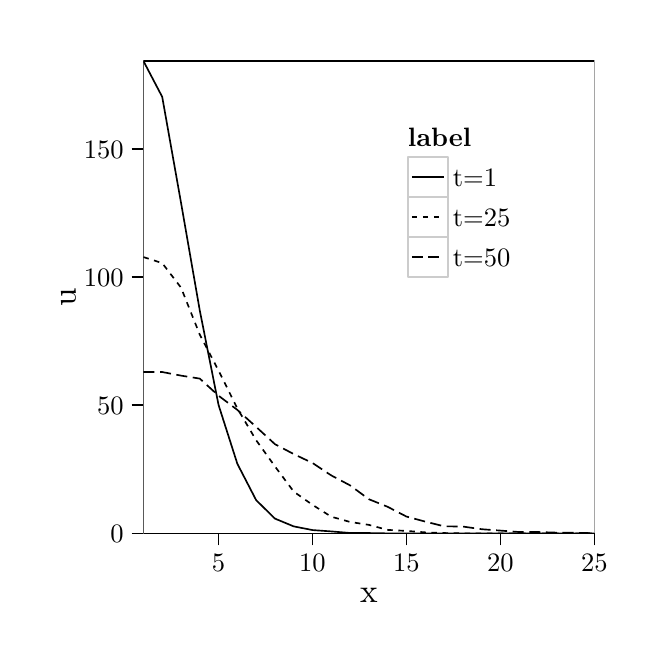
\begin{tikzpicture}[x=1pt,y=1pt]
\definecolor[named]{fillColor}{rgb}{1.00,1.00,1.00}
\path[use as bounding box,fill=fillColor,fill opacity=0.00] (0,0) rectangle (216.81,216.81);
\begin{scope}
\path[clip] (  0.00,  0.00) rectangle (216.81,216.81);
\definecolor[named]{drawColor}{rgb}{1.00,1.00,1.00}
\definecolor[named]{fillColor}{rgb}{1.00,1.00,1.00}

\path[draw=drawColor,line width= 0.6pt,line join=round,line cap=round,fill=fillColor] ( -0.00,  0.00) rectangle (216.81,216.81);
\end{scope}
\begin{scope}
\path[clip] ( 41.82, 34.03) rectangle (204.76,204.77);
\definecolor[named]{fillColor}{rgb}{1.00,1.00,1.00}

\path[fill=fillColor] ( 41.82, 34.03) rectangle (204.76,204.77);
\definecolor[named]{drawColor}{rgb}{0.00,0.00,0.00}

\path[draw=drawColor,line width= 0.6pt,line join=round] ( 41.82,204.77) --
	( 48.61,191.82) --
	( 55.40,153.62) --
	( 62.19,114.61) --
	( 68.98, 80.45) --
	( 75.77, 59.21) --
	( 82.56, 46.08) --
	( 89.35, 39.41) --
	( 96.13, 36.60) --
	(102.92, 35.27) --
	(109.71, 34.78) --
	(116.50, 34.22) --
	(123.29, 34.19) --
	(130.08, 34.07) --
	(136.87, 34.03) --
	(143.66, 34.03) --
	(150.45, 34.03) --
	(157.24, 34.03) --
	(164.03, 34.03) --
	(170.82, 34.03) --
	(177.61, 34.03) --
	(184.40, 34.03) --
	(191.19, 34.03) --
	(197.98, 34.03) --
	(204.76, 34.03);

\path[draw=drawColor,line width= 0.6pt,dash pattern=on 2pt off 2pt ,line join=round] ( 41.82,133.92) --
	( 48.61,131.75) --
	( 55.40,122.89) --
	( 62.19,105.90) --
	( 68.98, 92.87) --
	( 75.77, 79.22) --
	( 82.56, 67.73) --
	( 89.35, 58.28) --
	( 96.13, 49.17) --
	(102.92, 44.38) --
	(109.71, 40.09) --
	(116.50, 38.20) --
	(123.29, 37.15) --
	(130.08, 35.33) --
	(136.87, 34.96) --
	(143.66, 34.44) --
	(150.45, 34.19) --
	(157.24, 34.07) --
	(164.03, 34.03) --
	(170.82, 34.03) --
	(177.61, 34.03) --
	(184.40, 34.03) --
	(191.19, 34.03) --
	(197.98, 34.03) --
	(204.76, 34.03);

\path[draw=drawColor,line width= 0.6pt,dash pattern=on 4pt off 2pt ,line join=round] ( 41.82, 92.38) --
	( 48.61, 92.38) --
	( 55.40, 91.08) --
	( 62.19, 90.00) --
	( 68.98, 83.82) --
	( 75.77, 78.69) --
	( 82.56, 72.55) --
	( 89.35, 66.31) --
	( 96.13, 62.73) --
	(102.92, 59.51) --
	(109.71, 55.01) --
	(116.50, 51.42) --
	(123.29, 46.42) --
	(130.08, 43.67) --
	(136.87, 40.15) --
	(143.66, 38.33) --
	(150.45, 36.63) --
	(157.24, 36.54) --
	(164.03, 35.58) --
	(170.82, 35.08) --
	(177.61, 34.56) --
	(184.40, 34.56) --
	(191.19, 34.34) --
	(197.98, 34.28) --
	(204.76, 34.13);

\path[draw=drawColor,line width= 0.6pt,line join=round,line cap=round] ( 41.82, 34.03) rectangle (204.76,204.77);
\end{scope}
\begin{scope}
\path[clip] (  0.00,  0.00) rectangle (216.81,216.81);
\definecolor[named]{drawColor}{rgb}{0.00,0.00,0.00}

\node[text=drawColor,anchor=base east,inner sep=0pt, outer sep=0pt, scale=  0.96] at ( 34.71, 30.73) {0};

\node[text=drawColor,anchor=base east,inner sep=0pt, outer sep=0pt, scale=  0.96] at ( 34.71, 77.06) {50};

\node[text=drawColor,anchor=base east,inner sep=0pt, outer sep=0pt, scale=  0.96] at ( 34.71,123.38) {100};

\node[text=drawColor,anchor=base east,inner sep=0pt, outer sep=0pt, scale=  0.96] at ( 34.71,169.71) {150};
\end{scope}
\begin{scope}
\path[clip] (  0.00,  0.00) rectangle (216.81,216.81);
\definecolor[named]{drawColor}{rgb}{0.00,0.00,0.00}

\path[draw=drawColor,line width= 0.6pt,line join=round] ( 37.55, 34.03) --
	( 41.82, 34.03);

\path[draw=drawColor,line width= 0.6pt,line join=round] ( 37.55, 80.36) --
	( 41.82, 80.36);

\path[draw=drawColor,line width= 0.6pt,line join=round] ( 37.55,126.69) --
	( 41.82,126.69);

\path[draw=drawColor,line width= 0.6pt,line join=round] ( 37.55,173.02) --
	( 41.82,173.02);
\end{scope}
\begin{scope}
\path[clip] (  0.00,  0.00) rectangle (216.81,216.81);
\definecolor[named]{drawColor}{rgb}{0.00,0.00,0.00}

\path[draw=drawColor,line width= 0.6pt,line join=round] ( 68.98, 29.77) --
	( 68.98, 34.03);

\path[draw=drawColor,line width= 0.6pt,line join=round] (102.92, 29.77) --
	(102.92, 34.03);

\path[draw=drawColor,line width= 0.6pt,line join=round] (136.87, 29.77) --
	(136.87, 34.03);

\path[draw=drawColor,line width= 0.6pt,line join=round] (170.82, 29.77) --
	(170.82, 34.03);

\path[draw=drawColor,line width= 0.6pt,line join=round] (204.76, 29.77) --
	(204.76, 34.03);
\end{scope}
\begin{scope}
\path[clip] (  0.00,  0.00) rectangle (216.81,216.81);
\definecolor[named]{drawColor}{rgb}{0.00,0.00,0.00}

\node[text=drawColor,anchor=base,inner sep=0pt, outer sep=0pt, scale=  0.96] at ( 68.98, 20.31) {5};

\node[text=drawColor,anchor=base,inner sep=0pt, outer sep=0pt, scale=  0.96] at (102.92, 20.31) {10};

\node[text=drawColor,anchor=base,inner sep=0pt, outer sep=0pt, scale=  0.96] at (136.87, 20.31) {15};

\node[text=drawColor,anchor=base,inner sep=0pt, outer sep=0pt, scale=  0.96] at (170.82, 20.31) {20};

\node[text=drawColor,anchor=base,inner sep=0pt, outer sep=0pt, scale=  0.96] at (204.76, 20.31) {25};
\end{scope}
\begin{scope}
\path[clip] (  0.00,  0.00) rectangle (216.81,216.81);
\definecolor[named]{drawColor}{rgb}{0.00,0.00,0.00}

\node[text=drawColor,anchor=base,inner sep=0pt, outer sep=0pt, scale=  1.20] at (123.29,  9.03) {x};
\end{scope}
\begin{scope}
\path[clip] (  0.00,  0.00) rectangle (216.81,216.81);
\definecolor[named]{drawColor}{rgb}{0.00,0.00,0.00}

\node[text=drawColor,rotate= 90.00,anchor=base,inner sep=0pt, outer sep=0pt, scale=  1.20] at ( 17.30,119.40) {u};
\end{scope}
\begin{scope}
\path[clip] (  0.00,  0.00) rectangle (216.81,216.81);
\definecolor[named]{fillColor}{rgb}{1.00,1.00,1.00}

\path[fill=fillColor] (133.09,122.48) rectangle (178.68,184.61);
\end{scope}
\begin{scope}
\path[clip] (  0.00,  0.00) rectangle (216.81,216.81);
\definecolor[named]{drawColor}{rgb}{0.00,0.00,0.00}

\node[text=drawColor,anchor=base west,inner sep=0pt, outer sep=0pt, scale=  0.96] at (137.35,173.72) {\bfseries label};
\end{scope}
\begin{scope}
\path[clip] (  0.00,  0.00) rectangle (216.81,216.81);
\definecolor[named]{drawColor}{rgb}{0.80,0.80,0.80}
\definecolor[named]{fillColor}{rgb}{1.00,1.00,1.00}

\path[draw=drawColor,line width= 0.6pt,line join=round,line cap=round,fill=fillColor] (137.35,155.65) rectangle (151.81,170.11);
\end{scope}
\begin{scope}
\path[clip] (  0.00,  0.00) rectangle (216.81,216.81);
\definecolor[named]{drawColor}{rgb}{0.00,0.00,0.00}

\path[draw=drawColor,line width= 0.6pt,line join=round] (138.80,162.88) -- (150.36,162.88);
\end{scope}
\begin{scope}
\path[clip] (  0.00,  0.00) rectangle (216.81,216.81);
\definecolor[named]{drawColor}{rgb}{0.80,0.80,0.80}
\definecolor[named]{fillColor}{rgb}{1.00,1.00,1.00}

\path[draw=drawColor,line width= 0.6pt,line join=round,line cap=round,fill=fillColor] (137.35,141.20) rectangle (151.81,155.65);
\end{scope}
\begin{scope}
\path[clip] (  0.00,  0.00) rectangle (216.81,216.81);
\definecolor[named]{drawColor}{rgb}{0.00,0.00,0.00}

\path[draw=drawColor,line width= 0.6pt,dash pattern=on 2pt off 2pt ,line join=round] (138.80,148.43) -- (150.36,148.43);
\end{scope}
\begin{scope}
\path[clip] (  0.00,  0.00) rectangle (216.81,216.81);
\definecolor[named]{drawColor}{rgb}{0.80,0.80,0.80}
\definecolor[named]{fillColor}{rgb}{1.00,1.00,1.00}

\path[draw=drawColor,line width= 0.6pt,line join=round,line cap=round,fill=fillColor] (137.35,126.75) rectangle (151.81,141.20);
\end{scope}
\begin{scope}
\path[clip] (  0.00,  0.00) rectangle (216.81,216.81);
\definecolor[named]{drawColor}{rgb}{0.00,0.00,0.00}

\path[draw=drawColor,line width= 0.6pt,dash pattern=on 4pt off 2pt ,line join=round] (138.80,133.97) -- (150.36,133.97);
\end{scope}
\begin{scope}
\path[clip] (  0.00,  0.00) rectangle (216.81,216.81);
\definecolor[named]{drawColor}{rgb}{0.00,0.00,0.00}

\node[text=drawColor,anchor=base west,inner sep=0pt, outer sep=0pt, scale=  0.96] at (153.61,159.57) {t=1};
\end{scope}
\begin{scope}
\path[clip] (  0.00,  0.00) rectangle (216.81,216.81);
\definecolor[named]{drawColor}{rgb}{0.00,0.00,0.00}

\node[text=drawColor,anchor=base west,inner sep=0pt, outer sep=0pt, scale=  0.96] at (153.61,145.12) {t=25};
\end{scope}
\begin{scope}
\path[clip] (  0.00,  0.00) rectangle (216.81,216.81);
\definecolor[named]{drawColor}{rgb}{0.00,0.00,0.00}

\node[text=drawColor,anchor=base west,inner sep=0pt, outer sep=0pt, scale=  0.96] at (153.61,130.67) {t=50};
\end{scope}
\end{tikzpicture}

		%\caption{A common point cannot be found.}
	\end{subfigure}%
	\begin{subfigure}[h] {0.5 \textwidth}
		\input{NormedCOM.tex}
		%\caption{After normalisation a common point is found. }
	\end{subfigure}
	\caption{The center of mass frame for the cloud for both unnormalised and normalised data sets. Only the right hand half of the cloud is shown as it is assumed symmetric about the $y$ axis.}
\label{fig:NormedCOM}
\end{figure}

By examining the motion of such a point as shown in figure \ref{fig:NormedCOM} the velocity of the local motion of our cloud of mutations can be calculated.  

\begin{figure}[H]
	\begin{subfigure}[h]{0.5 \textwidth}
		% Created by tikzDevice version 0.7.0 on 2015-04-28 10:39:23
% !TEX encoding = UTF-8 Unicode
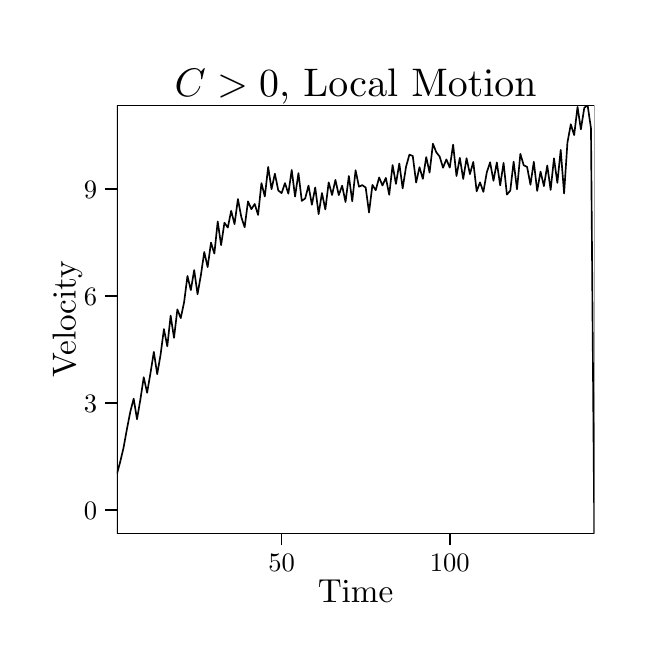
\begin{tikzpicture}[x=1pt,y=1pt]
\definecolor[named]{fillColor}{rgb}{1.00,1.00,1.00}
\path[use as bounding box,fill=fillColor,fill opacity=0.00] (0,0) rectangle (216.81,216.81);
\begin{scope}
\path[clip] (  0.00,  0.00) rectangle (216.81,216.81);
\definecolor[named]{drawColor}{rgb}{1.00,1.00,1.00}
\definecolor[named]{fillColor}{rgb}{1.00,1.00,1.00}

\path[draw=drawColor,line width= 0.6pt,line join=round,line cap=round,fill=fillColor] ( -0.00,  0.00) rectangle (216.81,216.81);
\end{scope}
\begin{scope}
\path[clip] ( 32.22, 34.03) rectangle (204.76,188.82);
\definecolor[named]{fillColor}{rgb}{1.00,1.00,1.00}

\path[fill=fillColor] ( 32.22, 34.03) rectangle (204.76,188.82);
\definecolor[named]{drawColor}{rgb}{0.00,0.00,0.00}

\path[draw=drawColor,line width= 0.6pt,line join=round] ( 32.22, 55.39) --
	( 33.44, 59.94) --
	( 34.65, 65.06) --
	( 35.87, 71.79) --
	( 37.08, 78.01) --
	( 38.30, 82.76) --
	( 39.51, 75.34) --
	( 40.73, 82.47) --
	( 41.94, 90.48) --
	( 43.16, 84.89) --
	( 44.37, 91.96) --
	( 45.59, 99.67) --
	( 46.80, 91.61) --
	( 48.02, 98.59) --
	( 49.23,107.90) --
	( 50.45,101.67) --
	( 51.66,112.73) --
	( 52.88,104.72) --
	( 54.09,115.01) --
	( 55.31,111.86) --
	( 56.52,117.58) --
	( 57.74,127.08) --
	( 58.95,121.99) --
	( 60.17,129.21) --
	( 61.38,120.48) --
	( 62.60,127.45) --
	( 63.81,135.75) --
	( 65.03,130.29) --
	( 66.24,139.12) --
	( 67.46,135.19) --
	( 68.67,146.76) --
	( 69.89,138.25) --
	( 71.10,146.33) --
	( 72.32,144.56) --
	( 73.53,150.63) --
	( 74.75,145.83) --
	( 75.97,154.88) --
	( 77.18,148.43) --
	( 78.40,144.70) --
	( 79.61,154.04) --
	( 80.83,151.23) --
	( 82.04,153.10) --
	( 83.26,149.14) --
	( 84.47,160.62) --
	( 85.69,155.80) --
	( 86.90,166.47) --
	( 88.12,158.46) --
	( 89.33,164.03) --
	( 90.55,157.98) --
	( 91.76,157.04) --
	( 92.98,160.65) --
	( 94.19,156.82) --
	( 95.41,165.39) --
	( 96.62,155.78) --
	( 97.84,164.25) --
	( 99.05,154.23) --
	(100.27,155.09) --
	(101.48,159.73) --
	(102.70,152.83) --
	(103.91,159.07) --
	(105.13,149.46) --
	(106.34,157.04) --
	(107.56,151.13) --
	(108.77,160.91) --
	(109.99,156.34) --
	(111.20,161.80) --
	(112.42,156.30) --
	(113.63,159.72) --
	(114.85,153.82) --
	(116.06,163.21) --
	(117.28,154.11) --
	(118.49,165.29) --
	(119.71,159.33) --
	(120.92,159.91) --
	(122.14,159.03) --
	(123.35,150.02) --
	(124.57,159.98) --
	(125.78,158.07) --
	(127.00,162.68) --
	(128.21,159.79) --
	(129.43,162.52) --
	(130.64,156.42) --
	(131.86,167.16) --
	(133.07,160.36) --
	(134.29,167.72) --
	(135.50,158.76) --
	(136.72,166.53) --
	(137.93,170.91) --
	(139.15,170.45) --
	(140.37,160.85) --
	(141.58,166.39) --
	(142.80,162.17) --
	(144.01,170.04) --
	(145.23,164.46) --
	(146.44,174.87) --
	(147.66,171.76) --
	(148.87,170.24) --
	(150.09,166.20) --
	(151.30,169.22) --
	(152.52,166.25) --
	(153.73,174.56) --
	(154.95,163.21) --
	(156.16,169.78) --
	(157.38,162.15) --
	(158.59,169.61) --
	(159.81,163.90) --
	(161.02,168.29) --
	(162.24,157.67) --
	(163.45,160.92) --
	(164.67,157.46) --
	(165.88,164.41) --
	(167.10,168.17) --
	(168.31,161.51) --
	(169.53,168.10) --
	(170.74,159.81) --
	(171.96,167.95) --
	(173.17,156.48) --
	(174.39,157.93) --
	(175.60,168.38) --
	(176.82,158.43) --
	(178.03,171.19) --
	(179.25,167.07) --
	(180.46,166.49) --
	(181.68,160.07) --
	(182.89,168.35) --
	(184.11,157.82) --
	(185.32,164.80) --
	(186.54,159.57) --
	(187.75,167.02) --
	(188.97,158.17) --
	(190.18,169.59) --
	(191.40,160.74) --
	(192.61,172.64) --
	(193.83,156.91) --
	(195.04,175.29) --
	(196.26,181.89) --
	(197.47,177.98) --
	(198.69,188.18) --
	(199.90,180.06) --
	(201.12,187.80) --
	(202.33,188.82) --
	(203.55,180.40) --
	(204.76, 34.03);

\path[draw=drawColor,line width= 0.6pt,line join=round,line cap=round] ( 32.22, 34.03) rectangle (204.76,188.82);
\end{scope}
\begin{scope}
\path[clip] (  0.00,  0.00) rectangle (216.81,216.81);
\definecolor[named]{drawColor}{rgb}{0.00,0.00,0.00}

\node[text=drawColor,anchor=base east,inner sep=0pt, outer sep=0pt, scale=  0.96] at ( 25.11, 39.15) {0};

\node[text=drawColor,anchor=base east,inner sep=0pt, outer sep=0pt, scale=  0.96] at ( 25.11, 77.81) {3};

\node[text=drawColor,anchor=base east,inner sep=0pt, outer sep=0pt, scale=  0.96] at ( 25.11,116.47) {6};

\node[text=drawColor,anchor=base east,inner sep=0pt, outer sep=0pt, scale=  0.96] at ( 25.11,155.12) {9};
\end{scope}
\begin{scope}
\path[clip] (  0.00,  0.00) rectangle (216.81,216.81);
\definecolor[named]{drawColor}{rgb}{0.00,0.00,0.00}

\path[draw=drawColor,line width= 0.6pt,line join=round] ( 27.95, 42.46) --
	( 32.22, 42.46);

\path[draw=drawColor,line width= 0.6pt,line join=round] ( 27.95, 81.12) --
	( 32.22, 81.12);

\path[draw=drawColor,line width= 0.6pt,line join=round] ( 27.95,119.77) --
	( 32.22,119.77);

\path[draw=drawColor,line width= 0.6pt,line join=round] ( 27.95,158.43) --
	( 32.22,158.43);
\end{scope}
\begin{scope}
\path[clip] (  0.00,  0.00) rectangle (216.81,216.81);
\definecolor[named]{drawColor}{rgb}{0.00,0.00,0.00}

\path[draw=drawColor,line width= 0.6pt,line join=round] ( 91.76, 29.77) --
	( 91.76, 34.03);

\path[draw=drawColor,line width= 0.6pt,line join=round] (152.52, 29.77) --
	(152.52, 34.03);
\end{scope}
\begin{scope}
\path[clip] (  0.00,  0.00) rectangle (216.81,216.81);
\definecolor[named]{drawColor}{rgb}{0.00,0.00,0.00}

\node[text=drawColor,anchor=base,inner sep=0pt, outer sep=0pt, scale=  0.96] at ( 91.76, 20.31) {50};

\node[text=drawColor,anchor=base,inner sep=0pt, outer sep=0pt, scale=  0.96] at (152.52, 20.31) {100};
\end{scope}
\begin{scope}
\path[clip] (  0.00,  0.00) rectangle (216.81,216.81);
\definecolor[named]{drawColor}{rgb}{0.00,0.00,0.00}

\node[text=drawColor,anchor=base,inner sep=0pt, outer sep=0pt, scale=  1.20] at (118.49,  9.03) {Time};
\end{scope}
\begin{scope}
\path[clip] (  0.00,  0.00) rectangle (216.81,216.81);
\definecolor[named]{drawColor}{rgb}{0.00,0.00,0.00}

\node[text=drawColor,rotate= 90.00,anchor=base,inner sep=0pt, outer sep=0pt, scale=  1.20] at ( 17.30,111.43) {Velocity};
\end{scope}
\begin{scope}
\path[clip] (  0.00,  0.00) rectangle (216.81,216.81);
\definecolor[named]{drawColor}{rgb}{0.00,0.00,0.00}

\node[text=drawColor,anchor=base,inner sep=0pt, outer sep=0pt, scale=  1.44] at (118.49,191.84) {$C > 0$, Local Motion};
\end{scope}
\end{tikzpicture}

		\caption{Local motion of our simulation.}
	\end{subfigure}
	\begin{subfigure}[h]{0.5 \textwidth}
		% Created by tikzDevice version 0.7.0 on 2015-04-28 10:39:40
% !TEX encoding = UTF-8 Unicode
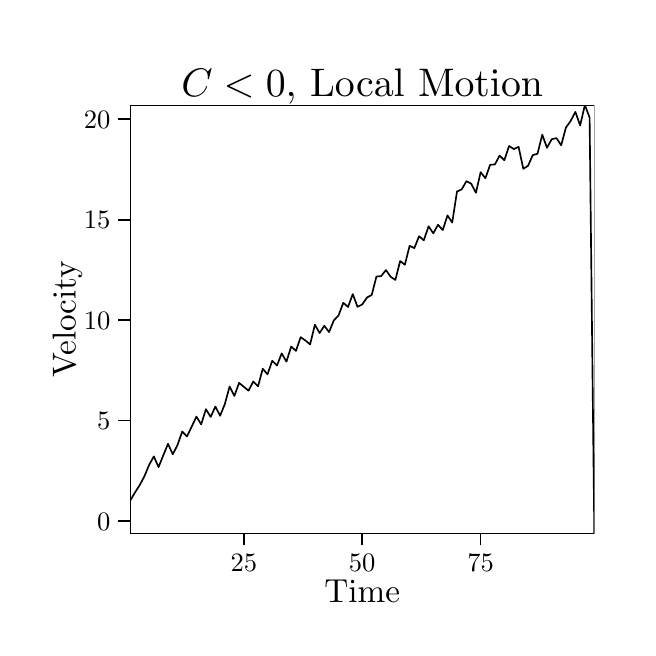
\begin{tikzpicture}[x=1pt,y=1pt]
\definecolor[named]{fillColor}{rgb}{1.00,1.00,1.00}
\path[use as bounding box,fill=fillColor,fill opacity=0.00] (0,0) rectangle (216.81,216.81);
\begin{scope}
\path[clip] (  0.00,  0.00) rectangle (216.81,216.81);
\definecolor[named]{drawColor}{rgb}{1.00,1.00,1.00}
\definecolor[named]{fillColor}{rgb}{1.00,1.00,1.00}

\path[draw=drawColor,line width= 0.6pt,line join=round,line cap=round,fill=fillColor] (  0.00,  0.00) rectangle (216.81,216.81);
\end{scope}
\begin{scope}
\path[clip] ( 37.02, 34.03) rectangle (204.76,188.82);
\definecolor[named]{fillColor}{rgb}{1.00,1.00,1.00}

\path[fill=fillColor] ( 37.02, 34.03) rectangle (204.76,188.82);
\definecolor[named]{drawColor}{rgb}{0.00,0.00,0.00}

\path[draw=drawColor,line width= 0.6pt,line join=round] ( 37.02, 45.88) --
	( 38.73, 48.76) --
	( 40.44, 51.45) --
	( 42.16, 54.66) --
	( 43.87, 58.79) --
	( 45.58, 61.89) --
	( 47.29, 58.01) --
	( 49.00, 62.26) --
	( 50.71, 66.44) --
	( 52.43, 62.65) --
	( 54.14, 66.01) --
	( 55.85, 70.87) --
	( 57.56, 69.09) --
	( 59.27, 72.66) --
	( 60.98, 76.26) --
	( 62.70, 73.48) --
	( 64.41, 78.94) --
	( 66.12, 76.16) --
	( 67.83, 79.91) --
	( 69.54, 76.57) --
	( 71.25, 80.81) --
	( 72.97, 87.16) --
	( 74.68, 83.73) --
	( 76.39, 88.45) --
	( 78.10, 87.05) --
	( 79.81, 85.64) --
	( 81.52, 88.96) --
	( 83.24, 87.19) --
	( 84.95, 93.57) --
	( 86.66, 91.54) --
	( 88.37, 96.45) --
	( 90.08, 94.73) --
	( 91.79, 99.11) --
	( 93.51, 96.13) --
	( 95.22,101.58) --
	( 96.93,100.01) --
	( 98.64,104.97) --
	(100.35,103.78) --
	(102.06,102.36) --
	(103.78,109.48) --
	(105.49,106.47) --
	(107.20,109.08) --
	(108.91,106.82) --
	(110.62,111.02) --
	(112.33,112.83) --
	(114.05,117.39) --
	(115.76,115.88) --
	(117.47,120.54) --
	(119.18,115.94) --
	(120.89,116.80) --
	(122.60,119.29) --
	(124.32,120.23) --
	(126.03,126.88) --
	(127.74,127.05) --
	(129.45,129.22) --
	(131.16,126.80) --
	(132.87,125.64) --
	(134.59,132.48) --
	(136.30,131.14) --
	(138.01,137.96) --
	(139.72,137.16) --
	(141.43,141.44) --
	(143.14,139.97) --
	(144.86,145.03) --
	(146.57,142.50) --
	(148.28,145.59) --
	(149.99,143.67) --
	(151.70,148.98) --
	(153.41,146.39) --
	(155.13,157.59) --
	(156.84,158.38) --
	(158.55,161.35) --
	(160.26,160.44) --
	(161.97,157.14) --
	(163.68,164.60) --
	(165.40,162.39) --
	(167.11,167.28) --
	(168.82,167.37) --
	(170.53,170.60) --
	(172.24,168.91) --
	(173.95,174.05) --
	(175.67,172.94) --
	(177.38,173.76) --
	(179.09,165.81) --
	(180.80,166.89) --
	(182.51,170.76) --
	(184.22,171.25) --
	(185.94,178.13) --
	(187.65,173.42) --
	(189.36,176.49) --
	(191.07,176.91) --
	(192.78,174.30) --
	(194.49,180.72) --
	(196.21,183.12) --
	(197.92,186.37) --
	(199.63,181.48) --
	(201.34,188.82) --
	(203.05,184.36) --
	(204.76, 34.03);

\path[draw=drawColor,line width= 0.6pt,line join=round,line cap=round] ( 37.02, 34.03) rectangle (204.76,188.82);
\end{scope}
\begin{scope}
\path[clip] (  0.00,  0.00) rectangle (216.81,216.81);
\definecolor[named]{drawColor}{rgb}{0.00,0.00,0.00}

\node[text=drawColor,anchor=base east,inner sep=0pt, outer sep=0pt, scale=  0.96] at ( 29.91, 35.19) {0};

\node[text=drawColor,anchor=base east,inner sep=0pt, outer sep=0pt, scale=  0.96] at ( 29.91, 71.49) {5};

\node[text=drawColor,anchor=base east,inner sep=0pt, outer sep=0pt, scale=  0.96] at ( 29.91,107.79) {10};

\node[text=drawColor,anchor=base east,inner sep=0pt, outer sep=0pt, scale=  0.96] at ( 29.91,144.10) {15};

\node[text=drawColor,anchor=base east,inner sep=0pt, outer sep=0pt, scale=  0.96] at ( 29.91,180.40) {20};
\end{scope}
\begin{scope}
\path[clip] (  0.00,  0.00) rectangle (216.81,216.81);
\definecolor[named]{drawColor}{rgb}{0.00,0.00,0.00}

\path[draw=drawColor,line width= 0.6pt,line join=round] ( 32.75, 38.50) --
	( 37.02, 38.50);

\path[draw=drawColor,line width= 0.6pt,line join=round] ( 32.75, 74.80) --
	( 37.02, 74.80);

\path[draw=drawColor,line width= 0.6pt,line join=round] ( 32.75,111.10) --
	( 37.02,111.10);

\path[draw=drawColor,line width= 0.6pt,line join=round] ( 32.75,147.40) --
	( 37.02,147.40);

\path[draw=drawColor,line width= 0.6pt,line join=round] ( 32.75,183.70) --
	( 37.02,183.70);
\end{scope}
\begin{scope}
\path[clip] (  0.00,  0.00) rectangle (216.81,216.81);
\definecolor[named]{drawColor}{rgb}{0.00,0.00,0.00}

\path[draw=drawColor,line width= 0.6pt,line join=round] ( 78.10, 29.77) --
	( 78.10, 34.03);

\path[draw=drawColor,line width= 0.6pt,line join=round] (120.89, 29.77) --
	(120.89, 34.03);

\path[draw=drawColor,line width= 0.6pt,line join=round] (163.68, 29.77) --
	(163.68, 34.03);
\end{scope}
\begin{scope}
\path[clip] (  0.00,  0.00) rectangle (216.81,216.81);
\definecolor[named]{drawColor}{rgb}{0.00,0.00,0.00}

\node[text=drawColor,anchor=base,inner sep=0pt, outer sep=0pt, scale=  0.96] at ( 78.10, 20.31) {25};

\node[text=drawColor,anchor=base,inner sep=0pt, outer sep=0pt, scale=  0.96] at (120.89, 20.31) {50};

\node[text=drawColor,anchor=base,inner sep=0pt, outer sep=0pt, scale=  0.96] at (163.68, 20.31) {75};
\end{scope}
\begin{scope}
\path[clip] (  0.00,  0.00) rectangle (216.81,216.81);
\definecolor[named]{drawColor}{rgb}{0.00,0.00,0.00}

\node[text=drawColor,anchor=base,inner sep=0pt, outer sep=0pt, scale=  1.20] at (120.89,  9.03) {Time};
\end{scope}
\begin{scope}
\path[clip] (  0.00,  0.00) rectangle (216.81,216.81);
\definecolor[named]{drawColor}{rgb}{0.00,0.00,0.00}

\node[text=drawColor,rotate= 90.00,anchor=base,inner sep=0pt, outer sep=0pt, scale=  1.20] at ( 17.30,111.43) {Velocity};
\end{scope}
\begin{scope}
\path[clip] (  0.00,  0.00) rectangle (216.81,216.81);
\definecolor[named]{drawColor}{rgb}{0.00,0.00,0.00}

\node[text=drawColor,anchor=base,inner sep=0pt, outer sep=0pt, scale=  1.44] at (120.89,191.84) {$C < 0$, Local Motion};
\end{scope}
\end{tikzpicture}

		\caption{Local motion of our simulation.}
	\end{subfigure}
	\caption{Comparisons of simulations with and without our differing mutation rates to test for Fisher Waves.}
	\label{fig:LocalMotionCancer}
\end{figure}

Figure \ref{fig:LocalMotionCancer} shows that by changing the mutation probability landscape a slight resemblance to the velocity profile that we would expect for Fisher waves (~figure~\ref{fig:FKKPVelocity}~) emerges. 
As expected for $C>0$ doesn't not produce Fisher waves and displays a constantly increasing velocity. This is expected as each subsequent mutation is easier to obtain, therefore the cloud expands quicker and locally progresses quicker. With a decreasing mutation landscape, $C < 0$,  a 'Fisher like' velocity occurs for the local motion. It increases before tapering off towards a constant. 

\begin{figure}[H]
	\centering
	\begin{subfigure}[h]{0.5 \textwidth}
		% Created by tikzDevice version 0.7.0 on 2015-04-30 13:17:13
% !TEX encoding = UTF-8 Unicode
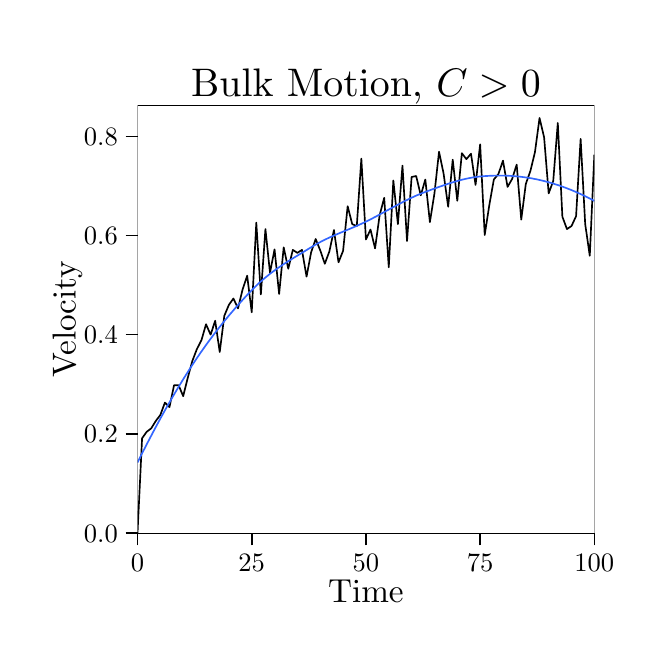
\begin{tikzpicture}[x=1pt,y=1pt]
\definecolor[named]{fillColor}{rgb}{1.00,1.00,1.00}
\path[use as bounding box,fill=fillColor,fill opacity=0.00] (0,0) rectangle (216.81,216.81);
\begin{scope}
\path[clip] (  0.00,  0.00) rectangle (216.81,216.81);
\definecolor[named]{drawColor}{rgb}{1.00,1.00,1.00}
\definecolor[named]{fillColor}{rgb}{1.00,1.00,1.00}

\path[draw=drawColor,line width= 0.6pt,line join=round,line cap=round,fill=fillColor] ( -0.00,  0.00) rectangle (216.81,216.81);
\end{scope}
\begin{scope}
\path[clip] ( 39.69, 34.03) rectangle (204.76,188.82);
\definecolor[named]{fillColor}{rgb}{1.00,1.00,1.00}

\path[fill=fillColor] ( 39.69, 34.03) rectangle (204.76,188.82);
\definecolor[named]{drawColor}{rgb}{0.00,0.00,0.00}

\path[draw=drawColor,line width= 0.6pt,line join=round] ( 39.69, 34.21) --
	( 41.34, 68.43) --
	( 42.99, 70.76) --
	( 44.64, 72.02) --
	( 46.29, 74.70) --
	( 47.94, 76.85) --
	( 49.59, 81.33) --
	( 51.24, 79.72) --
	( 52.89, 87.60) --
	( 54.54, 87.60) --
	( 56.19, 83.66) --
	( 57.85, 90.29) --
	( 59.50, 96.38) --
	( 61.15,100.68) --
	( 62.80,103.91) --
	( 64.45,109.64) --
	( 66.10,105.88) --
	( 67.75,110.89) --
	( 69.40, 99.61) --
	( 71.05,112.68) --
	( 72.70,116.63) --
	( 74.35,118.95) --
	( 76.00,115.37) --
	( 77.65,122.18) --
	( 79.31,127.20) --
	( 80.96,113.94) --
	( 82.61,146.37) --
	( 84.26,120.39) --
	( 85.91,144.04) --
	( 87.56,128.27) --
	( 89.21,136.69) --
	( 90.86,120.57) --
	( 92.51,137.41) --
	( 94.16,129.70) --
	( 95.81,136.51) --
	( 97.46,135.44) --
	( 99.11,136.51) --
	(100.77,126.84) --
	(102.42,135.62) --
	(104.07,140.45) --
	(105.72,136.33) --
	(107.37,131.50) --
	(109.02,135.97) --
	(110.67,143.68) --
	(112.32,132.03) --
	(113.97,136.15) --
	(115.62,152.28) --
	(117.27,145.83) --
	(118.92,145.11) --
	(120.57,169.48) --
	(122.23,140.27) --
	(123.88,143.86) --
	(125.53,137.05) --
	(127.18,149.05) --
	(128.83,155.32) --
	(130.48,130.24) --
	(132.13,161.59) --
	(133.78,145.83) --
	(135.43,166.97) --
	(137.08,139.74) --
	(138.73,162.85) --
	(140.38,163.21) --
	(142.04,156.22) --
	(143.69,161.95) --
	(145.34,146.54) --
	(146.99,156.94) --
	(148.64,171.98) --
	(150.29,164.10) --
	(151.94,152.10) --
	(153.59,169.12) --
	(155.24,154.25) --
	(156.89,171.45) --
	(158.54,169.30) --
	(160.19,171.27) --
	(161.84,159.98) --
	(163.50,174.67) --
	(165.15,141.89) --
	(166.80,152.64) --
	(168.45,161.95) --
	(170.10,163.92) --
	(171.75,168.76) --
	(173.40,159.26) --
	(175.05,162.13) --
	(176.70,167.33) --
	(178.35,147.44) --
	(180.00,160.34) --
	(181.65,165.00) --
	(183.30,171.81) --
	(184.96,184.17) --
	(186.61,177.18) --
	(188.26,156.94) --
	(189.91,161.41) --
	(191.56,182.38) --
	(193.21,148.51) --
	(194.86,144.04) --
	(196.51,145.11) --
	(198.16,148.69) --
	(199.81,176.64) --
	(201.46,145.83) --
	(203.11,134.36) --
	(204.76,170.91);

\path[] ( 39.69, 67.01) --
	( 41.78, 70.57) --
	( 43.87, 74.08) --
	( 45.96, 77.54) --
	( 48.04, 80.93) --
	( 50.13, 84.27) --
	( 52.22, 87.56) --
	( 54.31, 90.78) --
	( 56.40, 93.95) --
	( 58.49, 97.06) --
	( 60.58,100.10) --
	( 62.67,103.06) --
	( 64.76,105.93) --
	( 66.85,108.73) --
	( 68.94,111.45) --
	( 71.03,114.08) --
	( 73.12,116.63) --
	( 75.21,119.10) --
	( 77.30,121.49) --
	( 79.39,123.80) --
	( 81.48,126.04) --
	( 83.57,128.09) --
	( 85.66,129.93) --
	( 87.75,131.62) --
	( 89.84,133.18) --
	( 91.93,134.64) --
	( 94.02,136.03) --
	( 96.11,137.37) --
	( 98.20,138.69) --
	(100.28,139.99) --
	(102.37,141.29) --
	(104.46,142.50) --
	(106.55,143.55) --
	(108.64,144.50) --
	(110.73,145.39) --
	(112.82,146.28) --
	(114.91,147.17) --
	(117.00,148.10) --
	(119.09,149.07) --
	(121.18,150.06) --
	(123.27,151.08) --
	(125.36,152.12) --
	(127.45,153.17) --
	(129.54,154.24) --
	(131.63,155.34) --
	(133.72,156.46) --
	(135.81,157.58) --
	(137.90,158.69) --
	(139.99,159.74) --
	(142.08,160.68) --
	(144.17,161.50) --
	(146.26,162.24) --
	(148.35,162.95) --
	(150.44,163.63) --
	(152.52,164.28) --
	(154.61,164.88) --
	(156.70,165.43) --
	(158.79,165.91) --
	(160.88,166.28) --
	(162.97,166.54) --
	(165.06,166.67) --
	(167.15,166.75) --
	(169.24,166.77) --
	(171.33,166.73) --
	(173.42,166.65) --
	(175.51,166.51) --
	(177.60,166.33) --
	(179.69,166.10) --
	(181.78,165.84) --
	(183.87,165.55) --
	(185.96,165.23) --
	(188.05,164.88) --
	(190.14,164.52) --
	(192.23,164.15) --
	(194.32,163.76) --
	(196.41,163.36) --
	(198.50,162.94) --
	(200.59,162.50) --
	(202.68,162.04) --
	(204.76,161.55) --
	(204.76,146.89) --
	(202.68,148.57) --
	(200.59,150.14) --
	(198.50,151.60) --
	(196.41,152.95) --
	(194.32,154.18) --
	(192.23,155.29) --
	(190.14,156.28) --
	(188.05,157.14) --
	(185.96,157.88) --
	(183.87,158.50) --
	(181.78,158.99) --
	(179.69,159.38) --
	(177.60,159.67) --
	(175.51,159.86) --
	(173.42,159.97) --
	(171.33,159.99) --
	(169.24,159.95) --
	(167.15,159.83) --
	(165.06,159.66) --
	(162.97,159.43) --
	(160.88,159.11) --
	(158.79,158.69) --
	(156.70,158.18) --
	(154.61,157.58) --
	(152.52,156.90) --
	(150.44,156.16) --
	(148.35,155.37) --
	(146.26,154.57) --
	(144.17,153.78) --
	(142.08,153.00) --
	(139.99,152.16) --
	(137.90,151.25) --
	(135.81,150.27) --
	(133.72,149.21) --
	(131.63,148.08) --
	(129.54,146.90) --
	(127.45,145.69) --
	(125.36,144.51) --
	(123.27,143.38) --
	(121.18,142.36) --
	(119.09,141.46) --
	(117.00,140.63) --
	(114.91,139.81) --
	(112.82,138.97) --
	(110.73,138.07) --
	(108.64,137.08) --
	(106.55,136.00) --
	(104.46,134.83) --
	(102.37,133.57) --
	(100.28,132.31) --
	( 98.20,131.09) --
	( 96.11,129.87) --
	( 94.02,128.63) --
	( 91.93,127.32) --
	( 89.84,125.91) --
	( 87.75,124.39) --
	( 85.66,122.73) --
	( 83.57,120.91) --
	( 81.48,118.93) --
	( 79.39,116.79) --
	( 77.30,114.58) --
	( 75.21,112.28) --
	( 73.12,109.89) --
	( 71.03,107.40) --
	( 68.94,104.80) --
	( 66.85,102.08) --
	( 64.76, 99.22) --
	( 62.67, 96.21) --
	( 60.58, 93.05) --
	( 58.49, 89.71) --
	( 56.40, 86.21) --
	( 54.31, 82.53) --
	( 52.22, 78.69) --
	( 50.13, 74.69) --
	( 48.04, 70.52) --
	( 45.96, 66.20) --
	( 43.87, 61.72) --
	( 41.78, 57.10) --
	( 39.69, 52.34) --
	( 39.69, 67.01);
\definecolor[named]{drawColor}{rgb}{0.20,0.40,1.00}

\path[draw=drawColor,line width= 0.6pt,line join=round] ( 39.69, 59.68) --
	( 41.78, 63.84) --
	( 43.87, 67.90) --
	( 45.96, 71.87) --
	( 48.04, 75.73) --
	( 50.13, 79.48) --
	( 52.22, 83.12) --
	( 54.31, 86.66) --
	( 56.40, 90.08) --
	( 58.49, 93.38) --
	( 60.58, 96.57) --
	( 62.67, 99.63) --
	( 64.76,102.58) --
	( 66.85,105.40) --
	( 68.94,108.12) --
	( 71.03,110.74) --
	( 73.12,113.26) --
	( 75.21,115.69) --
	( 77.30,118.03) --
	( 79.39,120.30) --
	( 81.48,122.48) --
	( 83.57,124.50) --
	( 85.66,126.33) --
	( 87.75,128.01) --
	( 89.84,129.55) --
	( 91.93,130.98) --
	( 94.02,132.33) --
	( 96.11,133.62) --
	( 98.20,134.89) --
	(100.28,136.15) --
	(102.37,137.43) --
	(104.46,138.66) --
	(106.55,139.78) --
	(108.64,140.79) --
	(110.73,141.73) --
	(112.82,142.62) --
	(114.91,143.49) --
	(117.00,144.37) --
	(119.09,145.26) --
	(121.18,146.21) --
	(123.27,147.23) --
	(125.36,148.31) --
	(127.45,149.43) --
	(129.54,150.57) --
	(131.63,151.71) --
	(133.72,152.83) --
	(135.81,153.93) --
	(137.90,154.97) --
	(139.99,155.95) --
	(142.08,156.84) --
	(144.17,157.64) --
	(146.26,158.41) --
	(148.35,159.16) --
	(150.44,159.89) --
	(152.52,160.59) --
	(154.61,161.23) --
	(156.70,161.81) --
	(158.79,162.30) --
	(160.88,162.70) --
	(162.97,162.98) --
	(165.06,163.17) --
	(167.15,163.29) --
	(169.24,163.36) --
	(171.33,163.36) --
	(173.42,163.31) --
	(175.51,163.18) --
	(177.60,163.00) --
	(179.69,162.74) --
	(181.78,162.42) --
	(183.87,162.02) --
	(185.96,161.55) --
	(188.05,161.01) --
	(190.14,160.40) --
	(192.23,159.72) --
	(194.32,158.97) --
	(196.41,158.16) --
	(198.50,157.27) --
	(200.59,156.32) --
	(202.68,155.30) --
	(204.76,154.22);
\definecolor[named]{drawColor}{rgb}{0.00,0.00,0.00}

\path[draw=drawColor,line width= 0.6pt,line join=round,line cap=round] ( 39.69, 34.03) rectangle (204.76,188.82);
\end{scope}
\begin{scope}
\path[clip] (  0.00,  0.00) rectangle (216.81,216.81);
\definecolor[named]{drawColor}{rgb}{0.00,0.00,0.00}

\node[text=drawColor,anchor=base east,inner sep=0pt, outer sep=0pt, scale=  0.96] at ( 32.57, 30.91) {0.0};

\node[text=drawColor,anchor=base east,inner sep=0pt, outer sep=0pt, scale=  0.96] at ( 32.57, 66.74) {0.2};

\node[text=drawColor,anchor=base east,inner sep=0pt, outer sep=0pt, scale=  0.96] at ( 32.57,102.57) {0.4};

\node[text=drawColor,anchor=base east,inner sep=0pt, outer sep=0pt, scale=  0.96] at ( 32.57,138.40) {0.6};

\node[text=drawColor,anchor=base east,inner sep=0pt, outer sep=0pt, scale=  0.96] at ( 32.57,174.23) {0.8};
\end{scope}
\begin{scope}
\path[clip] (  0.00,  0.00) rectangle (216.81,216.81);
\definecolor[named]{drawColor}{rgb}{0.00,0.00,0.00}

\path[draw=drawColor,line width= 0.6pt,line join=round] ( 35.42, 34.21) --
	( 39.69, 34.21);

\path[draw=drawColor,line width= 0.6pt,line join=round] ( 35.42, 70.04) --
	( 39.69, 70.04);

\path[draw=drawColor,line width= 0.6pt,line join=round] ( 35.42,105.88) --
	( 39.69,105.88);

\path[draw=drawColor,line width= 0.6pt,line join=round] ( 35.42,141.71) --
	( 39.69,141.71);

\path[draw=drawColor,line width= 0.6pt,line join=round] ( 35.42,177.54) --
	( 39.69,177.54);
\end{scope}
\begin{scope}
\path[clip] (  0.00,  0.00) rectangle (216.81,216.81);
\definecolor[named]{drawColor}{rgb}{0.00,0.00,0.00}

\path[draw=drawColor,line width= 0.6pt,line join=round] ( 39.69, 29.77) --
	( 39.69, 34.03);

\path[draw=drawColor,line width= 0.6pt,line join=round] ( 80.96, 29.77) --
	( 80.96, 34.03);

\path[draw=drawColor,line width= 0.6pt,line join=round] (122.23, 29.77) --
	(122.23, 34.03);

\path[draw=drawColor,line width= 0.6pt,line join=round] (163.50, 29.77) --
	(163.50, 34.03);

\path[draw=drawColor,line width= 0.6pt,line join=round] (204.76, 29.77) --
	(204.76, 34.03);
\end{scope}
\begin{scope}
\path[clip] (  0.00,  0.00) rectangle (216.81,216.81);
\definecolor[named]{drawColor}{rgb}{0.00,0.00,0.00}

\node[text=drawColor,anchor=base,inner sep=0pt, outer sep=0pt, scale=  0.96] at ( 39.69, 20.31) {0};

\node[text=drawColor,anchor=base,inner sep=0pt, outer sep=0pt, scale=  0.96] at ( 80.96, 20.31) {25};

\node[text=drawColor,anchor=base,inner sep=0pt, outer sep=0pt, scale=  0.96] at (122.23, 20.31) {50};

\node[text=drawColor,anchor=base,inner sep=0pt, outer sep=0pt, scale=  0.96] at (163.50, 20.31) {75};

\node[text=drawColor,anchor=base,inner sep=0pt, outer sep=0pt, scale=  0.96] at (204.76, 20.31) {100};
\end{scope}
\begin{scope}
\path[clip] (  0.00,  0.00) rectangle (216.81,216.81);
\definecolor[named]{drawColor}{rgb}{0.00,0.00,0.00}

\node[text=drawColor,anchor=base,inner sep=0pt, outer sep=0pt, scale=  1.20] at (122.23,  9.03) {Time};
\end{scope}
\begin{scope}
\path[clip] (  0.00,  0.00) rectangle (216.81,216.81);
\definecolor[named]{drawColor}{rgb}{0.00,0.00,0.00}

\node[text=drawColor,rotate= 90.00,anchor=base,inner sep=0pt, outer sep=0pt, scale=  1.20] at ( 17.30,111.43) {Velocity};
\end{scope}
\begin{scope}
\path[clip] (  0.00,  0.00) rectangle (216.81,216.81);
\definecolor[named]{drawColor}{rgb}{0.00,0.00,0.00}

\node[text=drawColor,anchor=base,inner sep=0pt, outer sep=0pt, scale=  1.44] at (122.23,191.84) {Bulk Motion, $C > 0$};
\end{scope}
\end{tikzpicture}

	\end{subfigure}%
	\begin{subfigure}[h]{0.5 \textwidth}
		% Created by tikzDevice version 0.7.0 on 2015-04-30 13:17:14
% !TEX encoding = UTF-8 Unicode
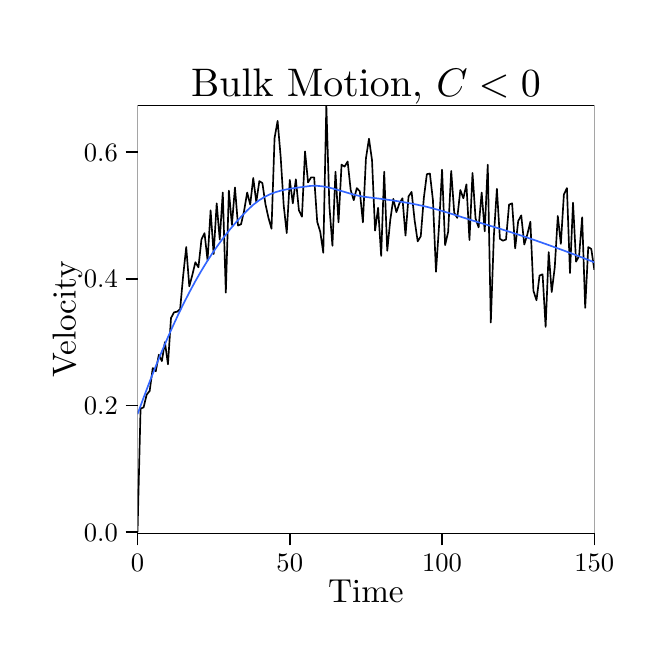
\begin{tikzpicture}[x=1pt,y=1pt]
\definecolor[named]{fillColor}{rgb}{1.00,1.00,1.00}
\path[use as bounding box,fill=fillColor,fill opacity=0.00] (0,0) rectangle (216.81,216.81);
\begin{scope}
\path[clip] (  0.00,  0.00) rectangle (216.81,216.81);
\definecolor[named]{drawColor}{rgb}{1.00,1.00,1.00}
\definecolor[named]{fillColor}{rgb}{1.00,1.00,1.00}

\path[draw=drawColor,line width= 0.6pt,line join=round,line cap=round,fill=fillColor] ( -0.00,  0.00) rectangle (216.81,216.81);
\end{scope}
\begin{scope}
\path[clip] ( 39.69, 34.03) rectangle (204.76,188.82);
\definecolor[named]{fillColor}{rgb}{1.00,1.00,1.00}

\path[fill=fillColor] ( 39.69, 34.03) rectangle (204.76,188.82);
\definecolor[named]{drawColor}{rgb}{0.00,0.00,0.00}

\path[draw=drawColor,line width= 0.6pt,line join=round] ( 39.69, 34.49) --
	( 40.79, 79.14) --
	( 41.89, 79.60) --
	( 42.99, 84.18) --
	( 44.09, 85.56) --
	( 45.19, 93.80) --
	( 46.29, 92.65) --
	( 47.39, 98.61) --
	( 48.49, 96.32) --
	( 49.59,103.19) --
	( 50.69, 95.17) --
	( 51.79,111.89) --
	( 52.89,113.95) --
	( 53.99,114.18) --
	( 55.09,115.09) --
	( 56.19,127.23) --
	( 57.29,137.53) --
	( 58.40,123.34) --
	( 59.50,127.46) --
	( 60.60,132.04) --
	( 61.70,130.21) --
	( 62.80,140.28) --
	( 63.90,142.57) --
	( 65.00,132.72) --
	( 66.10,150.81) --
	( 67.20,135.01) --
	( 68.30,153.33) --
	( 69.40,140.28) --
	( 70.50,157.23) --
	( 71.60,121.05) --
	( 72.70,157.91) --
	( 73.80,145.55) --
	( 74.90,159.06) --
	( 76.00,145.32) --
	( 77.10,145.78) --
	( 78.20,150.59) --
	( 79.31,157.23) --
	( 80.41,152.88) --
	( 81.51,162.49) --
	( 82.61,153.79) --
	( 83.71,161.35) --
	( 84.81,160.66) --
	( 85.91,153.10) --
	( 87.01,148.07) --
	( 88.11,144.17) --
	( 89.21,176.92) --
	( 90.31,183.10) --
	( 91.41,170.28) --
	( 92.51,152.65) --
	( 93.61,142.57) --
	( 94.71,161.81) --
	( 95.81,153.33) --
	( 96.91,162.03) --
	( 98.01,150.81) --
	( 99.11,148.52) --
	(100.22,172.11) --
	(101.32,160.89) --
	(102.42,162.72) --
	(103.52,162.72) --
	(104.62,146.69) --
	(105.72,143.03) --
	(106.82,135.47) --
	(107.92,188.82) --
	(109.02,152.42) --
	(110.12,137.99) --
	(111.22,164.78) --
	(112.32,146.46) --
	(113.42,167.30) --
	(114.52,166.61) --
	(115.62,168.45) --
	(116.72,158.14) --
	(117.82,154.48) --
	(118.92,158.83) --
	(120.02,157.68) --
	(121.13,146.46) --
	(122.23,169.59) --
	(123.33,176.69) --
	(124.43,168.90) --
	(125.53,143.49) --
	(126.63,151.73) --
	(127.73,134.33) --
	(128.83,164.78) --
	(129.93,136.16) --
	(131.03,147.38) --
	(132.13,154.94) --
	(133.23,150.13) --
	(134.33,153.33) --
	(135.43,155.16) --
	(136.53,141.66) --
	(137.63,155.85) --
	(138.73,157.45) --
	(139.83,147.15) --
	(140.93,139.59) --
	(142.04,141.43) --
	(143.14,155.16) --
	(144.24,163.87) --
	(145.34,164.10) --
	(146.44,154.48) --
	(147.54,128.60) --
	(148.64,145.09) --
	(149.74,165.47) --
	(150.84,138.22) --
	(151.94,143.03) --
	(153.04,165.01) --
	(154.14,149.90) --
	(155.24,148.07) --
	(156.34,158.14) --
	(157.44,155.16) --
	(158.54,160.20) --
	(159.64,140.05) --
	(160.74,164.32) --
	(161.84,147.84) --
	(162.95,144.63) --
	(164.05,157.23) --
	(165.15,143.26) --
	(166.25,167.30) --
	(167.35,110.28) --
	(168.45,141.43) --
	(169.55,158.60) --
	(170.65,140.51) --
	(171.75,139.82) --
	(172.85,140.28) --
	(173.95,152.88) --
	(175.05,153.33) --
	(176.15,137.08) --
	(177.25,146.92) --
	(178.35,148.98) --
	(179.45,138.45) --
	(180.55,142.11) --
	(181.65,146.69) --
	(182.75,121.73) --
	(183.86,118.30) --
	(184.96,127.23) --
	(186.06,127.69) --
	(187.16,108.68) --
	(188.26,135.70) --
	(189.36,121.28) --
	(190.46,130.21) --
	(191.56,148.75) --
	(192.66,138.68) --
	(193.76,156.54) --
	(194.86,158.83) --
	(195.96,128.15) --
	(197.06,153.56) --
	(198.16,132.27) --
	(199.26,134.33) --
	(200.36,148.30) --
	(201.46,115.55) --
	(202.56,137.53) --
	(203.66,136.85) --
	(204.76,129.29);

\path[] ( 39.69, 84.43) --
	( 41.78, 89.54) --
	( 43.87, 94.50) --
	( 45.96, 99.31) --
	( 48.04,103.97) --
	( 50.13,108.48) --
	( 52.22,112.84) --
	( 54.31,117.04) --
	( 56.40,121.09) --
	( 58.49,124.97) --
	( 60.58,128.68) --
	( 62.67,132.21) --
	( 64.76,135.56) --
	( 66.85,138.74) --
	( 68.94,141.74) --
	( 71.03,144.57) --
	( 73.12,147.24) --
	( 75.21,149.74) --
	( 77.30,152.08) --
	( 79.39,154.27) --
	( 81.48,156.27) --
	( 83.57,157.92) --
	( 85.66,159.23) --
	( 87.75,160.26) --
	( 89.84,161.05) --
	( 91.93,161.66) --
	( 94.02,162.14) --
	( 96.11,162.52) --
	( 98.20,162.85) --
	(100.28,163.16) --
	(102.37,163.43) --
	(104.46,163.42) --
	(106.55,163.15) --
	(108.64,162.70) --
	(110.73,162.14) --
	(112.82,161.54) --
	(114.91,160.94) --
	(117.00,160.39) --
	(119.09,159.92) --
	(121.18,159.55) --
	(123.27,159.28) --
	(125.36,158.98) --
	(127.45,158.66) --
	(129.54,158.32) --
	(131.63,157.99) --
	(133.72,157.68) --
	(135.81,157.37) --
	(137.90,157.07) --
	(139.99,156.73) --
	(142.08,156.34) --
	(144.17,155.86) --
	(146.26,155.31) --
	(148.35,154.69) --
	(150.44,154.03) --
	(152.52,153.35) --
	(154.61,152.67) --
	(156.70,151.98) --
	(158.79,151.29) --
	(160.88,150.61) --
	(162.97,149.94) --
	(165.06,149.27) --
	(167.15,148.60) --
	(169.24,147.92) --
	(171.33,147.23) --
	(173.42,146.55) --
	(175.51,145.87) --
	(177.60,145.19) --
	(179.69,144.54) --
	(181.78,143.90) --
	(183.87,143.30) --
	(185.96,142.72) --
	(188.05,142.18) --
	(190.14,141.69) --
	(192.23,141.24) --
	(194.32,140.83) --
	(196.41,140.46) --
	(198.50,140.12) --
	(200.59,139.83) --
	(202.68,139.56) --
	(204.76,139.32) --
	(204.76,124.73) --
	(202.68,126.15) --
	(200.59,127.51) --
	(198.50,128.82) --
	(196.41,130.08) --
	(194.32,131.27) --
	(192.23,132.40) --
	(190.14,133.47) --
	(188.05,134.48) --
	(185.96,135.42) --
	(183.87,136.31) --
	(181.78,137.13) --
	(179.69,137.91) --
	(177.60,138.64) --
	(175.51,139.33) --
	(173.42,139.99) --
	(171.33,140.62) --
	(169.24,141.23) --
	(167.15,141.82) --
	(165.06,142.39) --
	(162.97,142.97) --
	(160.88,143.57) --
	(158.79,144.21) --
	(156.70,144.85) --
	(154.61,145.49) --
	(152.52,146.11) --
	(150.44,146.70) --
	(148.35,147.26) --
	(146.26,147.79) --
	(144.17,148.29) --
	(142.08,148.77) --
	(139.99,149.25) --
	(137.90,149.72) --
	(135.81,150.15) --
	(133.72,150.52) --
	(131.63,150.84) --
	(129.54,151.09) --
	(127.45,151.31) --
	(125.36,151.50) --
	(123.27,151.71) --
	(121.18,151.98) --
	(119.09,152.44) --
	(117.00,153.04) --
	(114.91,153.72) --
	(112.82,154.39) --
	(110.73,154.99) --
	(108.64,155.47) --
	(106.55,155.80) --
	(104.46,155.94) --
	(102.37,155.86) --
	(100.28,155.59) --
	( 98.20,155.33) --
	( 96.11,155.09) --
	( 94.02,154.80) --
	( 91.93,154.41) --
	( 89.84,153.87) --
	( 87.75,153.13) --
	( 85.66,152.15) --
	( 83.57,150.88) --
	( 81.48,149.30) --
	( 79.39,147.39) --
	( 77.30,145.30) --
	( 75.21,143.04) --
	( 73.12,140.62) --
	( 71.03,138.01) --
	( 68.94,135.20) --
	( 66.85,132.18) --
	( 64.76,128.93) --
	( 62.67,125.44) --
	( 60.58,121.69) --
	( 58.49,117.67) --
	( 56.40,113.38) --
	( 54.31,108.82) --
	( 52.22,104.00) --
	( 50.13, 98.92) --
	( 48.04, 93.59) --
	( 45.96, 88.00) --
	( 43.87, 82.18) --
	( 41.78, 76.12) --
	( 39.69, 69.84) --
	( 39.69, 84.43);
\definecolor[named]{drawColor}{rgb}{0.20,0.40,1.00}

\path[draw=drawColor,line width= 0.6pt,line join=round] ( 39.69, 77.14) --
	( 41.78, 82.83) --
	( 43.87, 88.34) --
	( 45.96, 93.66) --
	( 48.04, 98.78) --
	( 50.13,103.70) --
	( 52.22,108.42) --
	( 54.31,112.93) --
	( 56.40,117.23) --
	( 58.49,121.32) --
	( 60.58,125.18) --
	( 62.67,128.82) --
	( 64.76,132.25) --
	( 66.85,135.46) --
	( 68.94,138.47) --
	( 71.03,141.29) --
	( 73.12,143.93) --
	( 75.21,146.39) --
	( 77.30,148.69) --
	( 79.39,150.83) --
	( 81.48,152.79) --
	( 83.57,154.40) --
	( 85.66,155.69) --
	( 87.75,156.69) --
	( 89.84,157.46) --
	( 91.93,158.04) --
	( 94.02,158.47) --
	( 96.11,158.81) --
	( 98.20,159.09) --
	(100.28,159.37) --
	(102.37,159.65) --
	(104.46,159.68) --
	(106.55,159.47) --
	(108.64,159.09) --
	(110.73,158.56) --
	(112.82,157.96) --
	(114.91,157.33) --
	(117.00,156.72) --
	(119.09,156.18) --
	(121.18,155.76) --
	(123.27,155.49) --
	(125.36,155.24) --
	(127.45,154.98) --
	(129.54,154.71) --
	(131.63,154.41) --
	(133.72,154.10) --
	(135.81,153.76) --
	(137.90,153.39) --
	(139.99,152.99) --
	(142.08,152.55) --
	(144.17,152.08) --
	(146.26,151.55) --
	(148.35,150.97) --
	(150.44,150.37) --
	(152.52,149.73) --
	(154.61,149.08) --
	(156.70,148.41) --
	(158.79,147.75) --
	(160.88,147.09) --
	(162.97,146.45) --
	(165.06,145.83) --
	(167.15,145.21) --
	(169.24,144.57) --
	(171.33,143.93) --
	(173.42,143.27) --
	(175.51,142.60) --
	(177.60,141.92) --
	(179.69,141.22) --
	(181.78,140.52) --
	(183.87,139.80) --
	(185.96,139.07) --
	(188.05,138.33) --
	(190.14,137.58) --
	(192.23,136.82) --
	(194.32,136.05) --
	(196.41,135.27) --
	(198.50,134.47) --
	(200.59,133.67) --
	(202.68,132.85) --
	(204.76,132.03);
\definecolor[named]{drawColor}{rgb}{0.00,0.00,0.00}

\path[draw=drawColor,line width= 0.6pt,line join=round,line cap=round] ( 39.69, 34.03) rectangle (204.76,188.82);
\end{scope}
\begin{scope}
\path[clip] (  0.00,  0.00) rectangle (216.81,216.81);
\definecolor[named]{drawColor}{rgb}{0.00,0.00,0.00}

\node[text=drawColor,anchor=base east,inner sep=0pt, outer sep=0pt, scale=  0.96] at ( 32.57, 31.19) {0.0};

\node[text=drawColor,anchor=base east,inner sep=0pt, outer sep=0pt, scale=  0.96] at ( 32.57, 76.98) {0.2};

\node[text=drawColor,anchor=base east,inner sep=0pt, outer sep=0pt, scale=  0.96] at ( 32.57,122.78) {0.4};

\node[text=drawColor,anchor=base east,inner sep=0pt, outer sep=0pt, scale=  0.96] at ( 32.57,168.57) {0.6};
\end{scope}
\begin{scope}
\path[clip] (  0.00,  0.00) rectangle (216.81,216.81);
\definecolor[named]{drawColor}{rgb}{0.00,0.00,0.00}

\path[draw=drawColor,line width= 0.6pt,line join=round] ( 35.42, 34.49) --
	( 39.69, 34.49);

\path[draw=drawColor,line width= 0.6pt,line join=round] ( 35.42, 80.29) --
	( 39.69, 80.29);

\path[draw=drawColor,line width= 0.6pt,line join=round] ( 35.42,126.08) --
	( 39.69,126.08);

\path[draw=drawColor,line width= 0.6pt,line join=round] ( 35.42,171.88) --
	( 39.69,171.88);
\end{scope}
\begin{scope}
\path[clip] (  0.00,  0.00) rectangle (216.81,216.81);
\definecolor[named]{drawColor}{rgb}{0.00,0.00,0.00}

\path[draw=drawColor,line width= 0.6pt,line join=round] ( 39.69, 29.77) --
	( 39.69, 34.03);

\path[draw=drawColor,line width= 0.6pt,line join=round] ( 94.71, 29.77) --
	( 94.71, 34.03);

\path[draw=drawColor,line width= 0.6pt,line join=round] (149.74, 29.77) --
	(149.74, 34.03);

\path[draw=drawColor,line width= 0.6pt,line join=round] (204.76, 29.77) --
	(204.76, 34.03);
\end{scope}
\begin{scope}
\path[clip] (  0.00,  0.00) rectangle (216.81,216.81);
\definecolor[named]{drawColor}{rgb}{0.00,0.00,0.00}

\node[text=drawColor,anchor=base,inner sep=0pt, outer sep=0pt, scale=  0.96] at ( 39.69, 20.31) {0};

\node[text=drawColor,anchor=base,inner sep=0pt, outer sep=0pt, scale=  0.96] at ( 94.71, 20.31) {50};

\node[text=drawColor,anchor=base,inner sep=0pt, outer sep=0pt, scale=  0.96] at (149.74, 20.31) {100};

\node[text=drawColor,anchor=base,inner sep=0pt, outer sep=0pt, scale=  0.96] at (204.76, 20.31) {150};
\end{scope}
\begin{scope}
\path[clip] (  0.00,  0.00) rectangle (216.81,216.81);
\definecolor[named]{drawColor}{rgb}{0.00,0.00,0.00}

\node[text=drawColor,anchor=base,inner sep=0pt, outer sep=0pt, scale=  1.20] at (122.23,  9.03) {Time};
\end{scope}
\begin{scope}
\path[clip] (  0.00,  0.00) rectangle (216.81,216.81);
\definecolor[named]{drawColor}{rgb}{0.00,0.00,0.00}

\node[text=drawColor,rotate= 90.00,anchor=base,inner sep=0pt, outer sep=0pt, scale=  1.20] at ( 17.30,111.43) {Velocity};
\end{scope}
\begin{scope}
\path[clip] (  0.00,  0.00) rectangle (216.81,216.81);
\definecolor[named]{drawColor}{rgb}{0.00,0.00,0.00}

\node[text=drawColor,anchor=base,inner sep=0pt, outer sep=0pt, scale=  1.44] at (122.23,191.84) {Bulk Motion, $C < 0$};
\end{scope}
\end{tikzpicture}

	\end{subfigure}
\end{figure}

\subsection{Analysing the shape of the wavefront}

As we have concluded that Fisher waves do not exist in our system it is a good idea to analyse where the analysis fails. 
The major assumption in the deviation is the small limit 

It is also desirable to test whether the wave front of our mutation cloud follows exponential decay. We follow the same process as previous used to show figure \ref{fig:FisherEXP}. 

\begin{figure}[H]
\begin{subfigure}[h]{0.5 \textwidth}
		% Created by tikzDevice version 0.7.0 on 2015-04-30 10:54:39
% !TEX encoding = UTF-8 Unicode
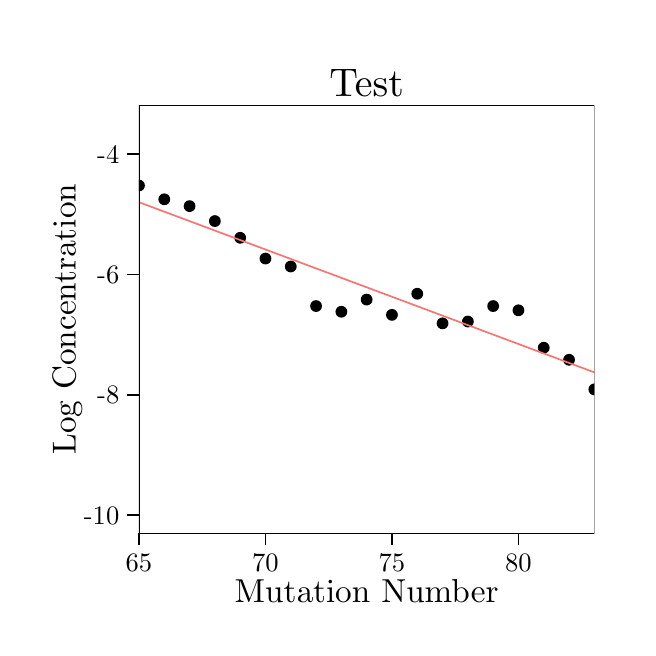
\begin{tikzpicture}[x=1pt,y=1pt]
\definecolor[named]{fillColor}{rgb}{1.00,1.00,1.00}
\path[use as bounding box,fill=fillColor,fill opacity=0.00] (0,0) rectangle (216.81,216.81);
\begin{scope}
\path[clip] (  0.00,  0.00) rectangle (216.81,216.81);
\definecolor[named]{drawColor}{rgb}{1.00,1.00,1.00}
\definecolor[named]{fillColor}{rgb}{1.00,1.00,1.00}

\path[draw=drawColor,line width= 0.6pt,line join=round,line cap=round,fill=fillColor] (  0.00,  0.00) rectangle (216.81,216.81);
\end{scope}
\begin{scope}
\path[clip] ( 40.22, 34.03) rectangle (204.76,188.82);
\definecolor[named]{fillColor}{rgb}{1.00,1.00,1.00}

\path[fill=fillColor] ( 40.22, 34.03) rectangle (204.76,188.82);
\definecolor[named]{fillColor}{rgb}{0.00,0.00,0.00}

\path[fill=fillColor] ( 40.22,159.77) circle (  2.13);

\path[fill=fillColor] ( 49.36,154.79) circle (  2.13);

\path[fill=fillColor] ( 58.50,152.32) circle (  2.13);

\path[fill=fillColor] ( 67.64,146.93) circle (  2.13);

\path[fill=fillColor] ( 76.79,140.88) circle (  2.13);

\path[fill=fillColor] ( 85.93,133.38) circle (  2.13);

\path[fill=fillColor] ( 95.07,130.51) circle (  2.13);

\path[fill=fillColor] (104.21,116.21) circle (  2.13);

\path[fill=fillColor] (113.35,114.15) circle (  2.13);

\path[fill=fillColor] (122.49,118.55) circle (  2.13);

\path[fill=fillColor] (131.63,113.03) circle (  2.13);

\path[fill=fillColor] (140.78,120.66) circle (  2.13);

\path[fill=fillColor] (149.92,109.97) circle (  2.13);

\path[fill=fillColor] (159.06,110.62) circle (  2.13);

\path[fill=fillColor] (168.20,116.21) circle (  2.13);

\path[fill=fillColor] (177.34,114.68) circle (  2.13);

\path[fill=fillColor] (186.48,101.16) circle (  2.13);

\path[fill=fillColor] (195.62, 96.80) circle (  2.13);

\path[fill=fillColor] (204.76, 86.11) circle (  2.13);
\definecolor[named]{drawColor}{rgb}{0.97,0.46,0.43}
\definecolor[named]{fillColor}{rgb}{0.97,0.46,0.43}

\path[draw=drawColor,line width= 0.6pt,line join=round,fill=fillColor] ( 40.22,153.73) -- (204.76, 92.25);
\definecolor[named]{drawColor}{rgb}{0.00,0.00,0.00}

\path[draw=drawColor,line width= 0.6pt,line join=round,line cap=round] ( 40.22, 34.03) rectangle (204.76,188.82);
\end{scope}
\begin{scope}
\path[clip] (  0.00,  0.00) rectangle (216.81,216.81);
\definecolor[named]{drawColor}{rgb}{0.00,0.00,0.00}

\node[text=drawColor,anchor=base east,inner sep=0pt, outer sep=0pt, scale=  0.96] at ( 33.11, 37.44) {-10};

\node[text=drawColor,anchor=base east,inner sep=0pt, outer sep=0pt, scale=  0.96] at ( 33.11, 80.87) {-8};

\node[text=drawColor,anchor=base east,inner sep=0pt, outer sep=0pt, scale=  0.96] at ( 33.11,124.31) {-6};

\node[text=drawColor,anchor=base east,inner sep=0pt, outer sep=0pt, scale=  0.96] at ( 33.11,167.74) {-4};
\end{scope}
\begin{scope}
\path[clip] (  0.00,  0.00) rectangle (216.81,216.81);
\definecolor[named]{drawColor}{rgb}{0.00,0.00,0.00}

\path[draw=drawColor,line width= 0.6pt,line join=round] ( 35.95, 40.74) --
	( 40.22, 40.74);

\path[draw=drawColor,line width= 0.6pt,line join=round] ( 35.95, 84.18) --
	( 40.22, 84.18);

\path[draw=drawColor,line width= 0.6pt,line join=round] ( 35.95,127.61) --
	( 40.22,127.61);

\path[draw=drawColor,line width= 0.6pt,line join=round] ( 35.95,171.04) --
	( 40.22,171.04);
\end{scope}
\begin{scope}
\path[clip] (  0.00,  0.00) rectangle (216.81,216.81);
\definecolor[named]{drawColor}{rgb}{0.00,0.00,0.00}

\path[draw=drawColor,line width= 0.6pt,line join=round] ( 40.22, 29.77) --
	( 40.22, 34.03);

\path[draw=drawColor,line width= 0.6pt,line join=round] ( 85.93, 29.77) --
	( 85.93, 34.03);

\path[draw=drawColor,line width= 0.6pt,line join=round] (131.63, 29.77) --
	(131.63, 34.03);

\path[draw=drawColor,line width= 0.6pt,line join=round] (177.34, 29.77) --
	(177.34, 34.03);
\end{scope}
\begin{scope}
\path[clip] (  0.00,  0.00) rectangle (216.81,216.81);
\definecolor[named]{drawColor}{rgb}{0.00,0.00,0.00}

\node[text=drawColor,anchor=base,inner sep=0pt, outer sep=0pt, scale=  0.96] at ( 40.22, 20.31) {65};

\node[text=drawColor,anchor=base,inner sep=0pt, outer sep=0pt, scale=  0.96] at ( 85.93, 20.31) {70};

\node[text=drawColor,anchor=base,inner sep=0pt, outer sep=0pt, scale=  0.96] at (131.63, 20.31) {75};

\node[text=drawColor,anchor=base,inner sep=0pt, outer sep=0pt, scale=  0.96] at (177.34, 20.31) {80};
\end{scope}
\begin{scope}
\path[clip] (  0.00,  0.00) rectangle (216.81,216.81);
\definecolor[named]{drawColor}{rgb}{0.00,0.00,0.00}

\node[text=drawColor,anchor=base,inner sep=0pt, outer sep=0pt, scale=  1.20] at (122.49,  9.03) {Mutation Number};
\end{scope}
\begin{scope}
\path[clip] (  0.00,  0.00) rectangle (216.81,216.81);
\definecolor[named]{drawColor}{rgb}{0.00,0.00,0.00}

\node[text=drawColor,rotate= 90.00,anchor=base,inner sep=0pt, outer sep=0pt, scale=  1.20] at ( 17.30,111.43) {Log Concentration};
\end{scope}
\begin{scope}
\path[clip] (  0.00,  0.00) rectangle (216.81,216.81);
\definecolor[named]{drawColor}{rgb}{0.00,0.00,0.00}

\node[text=drawColor,anchor=base,inner sep=0pt, outer sep=0pt, scale=  1.44] at (122.49,191.84) {Test};
\end{scope}
\end{tikzpicture}

	\caption{Checking exp for positive simulation}
\end{subfigure}
\begin{subfigure}[h]{0.5 \textwidth}
		% Created by tikzDevice version 0.7.0 on 2015-04-30 08:26:53
% !TEX encoding = UTF-8 Unicode
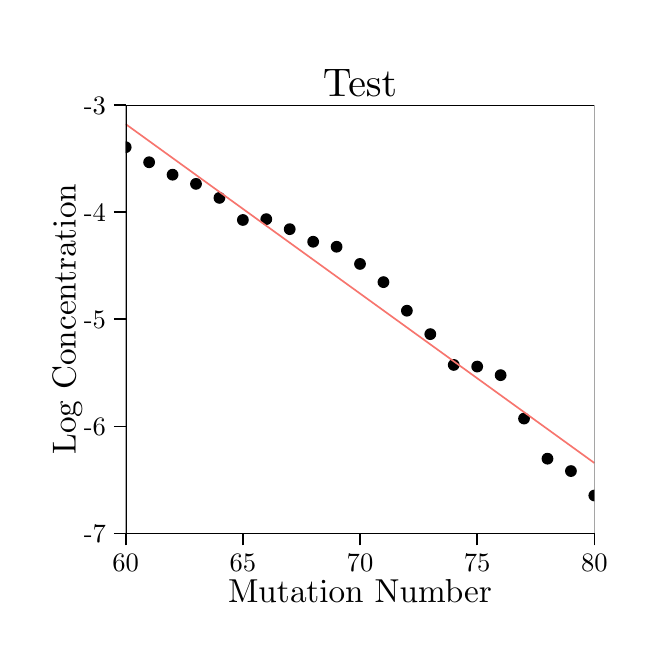
\begin{tikzpicture}[x=1pt,y=1pt]
\definecolor[named]{fillColor}{rgb}{1.00,1.00,1.00}
\path[use as bounding box,fill=fillColor,fill opacity=0.00] (0,0) rectangle (216.81,216.81);
\begin{scope}
\path[clip] (  0.00,  0.00) rectangle (216.81,216.81);
\definecolor[named]{drawColor}{rgb}{1.00,1.00,1.00}
\definecolor[named]{fillColor}{rgb}{1.00,1.00,1.00}

\path[draw=drawColor,line width= 0.6pt,line join=round,line cap=round,fill=fillColor] (  0.00,  0.00) rectangle (216.81,216.81);
\end{scope}
\begin{scope}
\path[clip] ( 35.42, 34.03) rectangle (204.76,188.82);
\definecolor[named]{fillColor}{rgb}{1.00,1.00,1.00}

\path[fill=fillColor] ( 35.42, 34.03) rectangle (204.76,188.82);
\definecolor[named]{fillColor}{rgb}{0.00,0.00,0.00}

\path[fill=fillColor] ( 35.42,173.61) circle (  2.13);

\path[fill=fillColor] ( 43.89,168.18) circle (  2.13);

\path[fill=fillColor] ( 52.36,163.68) circle (  2.13);

\path[fill=fillColor] ( 60.82,160.37) circle (  2.13);

\path[fill=fillColor] ( 69.29,155.30) circle (  2.13);

\path[fill=fillColor] ( 77.76,147.32) circle (  2.13);

\path[fill=fillColor] ( 86.22,147.62) circle (  2.13);

\path[fill=fillColor] ( 94.69,144.00) circle (  2.13);

\path[fill=fillColor] (103.16,139.45) circle (  2.13);

\path[fill=fillColor] (111.63,137.65) circle (  2.13);

\path[fill=fillColor] (120.09,131.44) circle (  2.13);

\path[fill=fillColor] (128.56,124.86) circle (  2.13);

\path[fill=fillColor] (137.03,114.53) circle (  2.13);

\path[fill=fillColor] (145.49,106.07) circle (  2.13);

\path[fill=fillColor] (153.96, 94.94) circle (  2.13);

\path[fill=fillColor] (162.43, 94.35) circle (  2.13);

\path[fill=fillColor] (170.90, 91.25) circle (  2.13);

\path[fill=fillColor] (179.36, 75.56) circle (  2.13);

\path[fill=fillColor] (187.83, 61.06) circle (  2.13);

\path[fill=fillColor] (196.30, 56.59) circle (  2.13);

\path[fill=fillColor] (204.76, 47.76) circle (  2.13);
\definecolor[named]{drawColor}{rgb}{0.97,0.46,0.43}
\definecolor[named]{fillColor}{rgb}{0.97,0.46,0.43}

\path[draw=drawColor,line width= 0.6pt,line join=round,fill=fillColor] ( 35.42,181.96) -- (204.76, 59.52);
\definecolor[named]{drawColor}{rgb}{0.00,0.00,0.00}

\path[draw=drawColor,line width= 0.6pt,line join=round,line cap=round] ( 35.42, 34.03) rectangle (204.76,188.82);
\end{scope}
\begin{scope}
\path[clip] (  0.00,  0.00) rectangle (216.81,216.81);
\definecolor[named]{drawColor}{rgb}{0.00,0.00,0.00}

\node[text=drawColor,anchor=base east,inner sep=0pt, outer sep=0pt, scale=  0.96] at ( 28.31, 30.73) {-7};

\node[text=drawColor,anchor=base east,inner sep=0pt, outer sep=0pt, scale=  0.96] at ( 28.31, 69.43) {-6};

\node[text=drawColor,anchor=base east,inner sep=0pt, outer sep=0pt, scale=  0.96] at ( 28.31,108.12) {-5};

\node[text=drawColor,anchor=base east,inner sep=0pt, outer sep=0pt, scale=  0.96] at ( 28.31,146.82) {-4};

\node[text=drawColor,anchor=base east,inner sep=0pt, outer sep=0pt, scale=  0.96] at ( 28.31,185.52) {-3};
\end{scope}
\begin{scope}
\path[clip] (  0.00,  0.00) rectangle (216.81,216.81);
\definecolor[named]{drawColor}{rgb}{0.00,0.00,0.00}

\path[draw=drawColor,line width= 0.6pt,line join=round] ( 31.15, 34.03) --
	( 35.42, 34.03);

\path[draw=drawColor,line width= 0.6pt,line join=round] ( 31.15, 72.73) --
	( 35.42, 72.73);

\path[draw=drawColor,line width= 0.6pt,line join=round] ( 31.15,111.43) --
	( 35.42,111.43);

\path[draw=drawColor,line width= 0.6pt,line join=round] ( 31.15,150.13) --
	( 35.42,150.13);

\path[draw=drawColor,line width= 0.6pt,line join=round] ( 31.15,188.82) --
	( 35.42,188.82);
\end{scope}
\begin{scope}
\path[clip] (  0.00,  0.00) rectangle (216.81,216.81);
\definecolor[named]{drawColor}{rgb}{0.00,0.00,0.00}

\path[draw=drawColor,line width= 0.6pt,line join=round] ( 35.42, 29.77) --
	( 35.42, 34.03);

\path[draw=drawColor,line width= 0.6pt,line join=round] ( 77.76, 29.77) --
	( 77.76, 34.03);

\path[draw=drawColor,line width= 0.6pt,line join=round] (120.09, 29.77) --
	(120.09, 34.03);

\path[draw=drawColor,line width= 0.6pt,line join=round] (162.43, 29.77) --
	(162.43, 34.03);

\path[draw=drawColor,line width= 0.6pt,line join=round] (204.76, 29.77) --
	(204.76, 34.03);
\end{scope}
\begin{scope}
\path[clip] (  0.00,  0.00) rectangle (216.81,216.81);
\definecolor[named]{drawColor}{rgb}{0.00,0.00,0.00}

\node[text=drawColor,anchor=base,inner sep=0pt, outer sep=0pt, scale=  0.96] at ( 35.42, 20.31) {60};

\node[text=drawColor,anchor=base,inner sep=0pt, outer sep=0pt, scale=  0.96] at ( 77.76, 20.31) {65};

\node[text=drawColor,anchor=base,inner sep=0pt, outer sep=0pt, scale=  0.96] at (120.09, 20.31) {70};

\node[text=drawColor,anchor=base,inner sep=0pt, outer sep=0pt, scale=  0.96] at (162.43, 20.31) {75};

\node[text=drawColor,anchor=base,inner sep=0pt, outer sep=0pt, scale=  0.96] at (204.76, 20.31) {80};
\end{scope}
\begin{scope}
\path[clip] (  0.00,  0.00) rectangle (216.81,216.81);
\definecolor[named]{drawColor}{rgb}{0.00,0.00,0.00}

\node[text=drawColor,anchor=base,inner sep=0pt, outer sep=0pt, scale=  1.20] at (120.09,  9.03) {Mutation Number};
\end{scope}
\begin{scope}
\path[clip] (  0.00,  0.00) rectangle (216.81,216.81);
\definecolor[named]{drawColor}{rgb}{0.00,0.00,0.00}

\node[text=drawColor,rotate= 90.00,anchor=base,inner sep=0pt, outer sep=0pt, scale=  1.20] at ( 17.30,111.43) {Log Concentration};
\end{scope}
\begin{scope}
\path[clip] (  0.00,  0.00) rectangle (216.81,216.81);
\definecolor[named]{drawColor}{rgb}{0.00,0.00,0.00}

\node[text=drawColor,anchor=base,inner sep=0pt, outer sep=0pt, scale=  1.44] at (120.09,191.84) {Test};
\end{scope}
\end{tikzpicture}

	\caption{Checking exp for negative simulation}
\end{subfigure}
\caption{Checking the shape of the wavefront for a single moment in time. The linear fit is calculated using R's `lm' function.  }
\end{figure}

\begin{figure}[H]
\centering
	\begin{subfigure}[h]{0.5 \textwidth}
		\input{res_data_pos.tex}
	\end{subfigure}%
	\begin{subfigure}[h]{0.5 \textwidth}
		\input{res_data_neg.tex}
	\end{subfigure}
\end{figure}

\begin{figure}[H]
\centering
\input{res_data_flat.tex}
\end{figure}

\subsection{Fisher Wave Conclusions}

By following the same analysis as Fisher we have shown that both the bulk motion of our mutation cloud and the local motion of it diffusing are not Fisher waves.  

\newpage



\section{Conclusion}

Overall, we have successfully analysed the dynamics of cancer evolution using both a computational approach and an analytical method. 

We have extended our simulation to account for a variable mutation probability landscape and successfully obtained a number of new data sets.

We also extended our analytic analysis to a non-constant mutation probability landscape and derived both the discrete and continuous equations that govern the evolution of the population numbers. In the case of constant fitness but non-constant mutation probability we successfully reduced the problem to the diffusion equation with a non constant diffusion constant.

By drawing from the previous work of Fisher et al. we derived suitable criteria on the mutation landscape for the existence of Fisher waves within our system. Using numerical integration techniques we were able to include both cases of the mutation landscape in our simulation. The results of these simulations lead us to conclude that both the bulk progression of the wave and the local dispersion of the wave away from the centre of mass are not Fisher waves. By looking at the shape of the wave front we found that the key assumption of a exponentially decaying wave front was not true and as such explains why a constant velocity of progression was not found. 

\subsection{Further Work}

%With regards to the diffusion equation, we will extend the derivation to account for an inhomogeneous landscape for both fitness and mutation probabilities. This will require introducing non-linear terms into the diffusion equation, notably the $\bar{r}$ term in equation \eqref{eq:MasterSimple}. More complex techniques will have to be used to solve this type of equation, as Fourier methods will no longer prove feasible. Our first attempts will involve a mean-field approximation of the populations as time progresses. 
%This will provide a more accurate model of cancer, as biologically, a larger number of mutations will have an adverse effect on the health and properties of the cell, therefore the fitness values and mutation probabilities will not all be equal. 

To extend the scope of the simulation, it would interesting to replicate the human body more accurately. This would be achieved by setting up multiple populations of cells and creating rules that allow transfer of mutants from one population to another. This would mimic human biology better, as internally, humans have many different cell types that interact with each other in specific ways. It would then be possible to see both the development of mutations locally within a population group and how the mutations propagated through a connected network of populations. 
It would also be interesting to obtain experimental data from lab grown cancer cells to test the application of the Moran process and how accurate it is in describing cancer growth. 

\newpage

\printbibliography

\newpage

\section*{Risk Assessment for Stochastic Dynamics of Cancer \\ Evolution MPhys Project}


This project consists of building computer simulations to model the dynamics of cancer. Therefore, the majority of work will be done using a University computer or personal laptop. The work will be carried out in the Schuster Laboratory and the students homes. 


\subsection*{Hazards}

We have identified the following as our main hazards. 

\begin{enumerate}
\item Repetitive strain injury (RSI) from using keyboard and mouse. 
\item Display screen equipment causing eyestrain after prolonged use.
\item Fire risk from the electrical charging equipment of our laptops. 
\item Electrical equipment. 
\item Obstructions providing a trip/fall risk.
\end{enumerate}

\subsection*{Potential Victims}

Items 1 and 2 concern both partners working on the project, without posing any risk to other people. However, items 3, 4 and 5 are a public hazard effecting not only the partners but surrounding people in the Schuster Laboratory.  

\subsection*{Risk Evaluation}

All the above risks are insignificant and can be adequately controlled by following both the University guidelines and ensuring that the current safety guidelines are followed. 

\subsection*{Actions to be taken}

Both persons working on the project need to ensure that this risk assessment is read and ensure that they follow the University guidelines. 

\subsection*{Review}

This risk assessment will be revised if there is change to the project brief. 

\subsection*{Record}

This risk assessment was carried out on 23/09/14 by Dean Markwick and Matthew de Angelis.  

%\pagenumbering{gobble}

\end{document}
